%=======================================================================
%  PRINCIPLES OF CONTINUUM MECHANICS -- study notes
%  Chapters 1-12 after Steigmann & Shirani, assembled into one document.
%
%  The chapter bodies live in  body_ch1.tex ... body_ch12.tex and are
%  generated from the standalone chapter files; the preamble below is
%  their union.  Problems appear in the table of contents and hence in
%  the PDF bookmarks.
%
%  Compile:  latexmk -pdf main.tex
%=======================================================================
\documentclass[17pt,a4paper,openany]{extreport}

\usepackage[margin=1.8cm]{geometry}
\usepackage{amsmath,amssymb,amsthm}
\usepackage{bm}
\usepackage{accents}
% book style: boldface is rendered by an under-tilde
\DeclareRobustCommand{\vek}[1]{\underaccent{\tilde}{#1}}
\usepackage{xcolor}
\usepackage{enumitem}
\usepackage{graphicx}
\usepackage{array}
\usepackage{tikz}
\usetikzlibrary{arrows.meta,calc,positioning,angles,quotes,patterns}
\usepackage{pgfplots}
\pgfplotsset{compat=1.18}
\tikzset{vec/.style={-{Stealth[length=2.3mm]},thick},
         thinvec/.style={-{Stealth[length=1.8mm]},semithick},
         mapar/.style={-{Stealth[length=2.4mm]},thick},
         guide/.style={gray!65,densely dashed,thin},
         bodyline/.style={thick,dashed},
         configline/.style={thick},
         lbl/.style={fill=white,inner sep=1pt}}
\newcommand{\blob}[1]{\draw[#1] plot[smooth cycle,tension=0.85] coordinates
  {(0,1.05) (1.15,0.72) (1.5,-0.35) (0.6,-1.15) (-0.75,-0.95) (-1.3,0.05)};}
\usepackage[colorlinks=true,linkcolor=blue!55!black,citecolor=blue!55!black,
            hypertexnames=false,pdfencoding=unicode,
            bookmarksnumbered=true,bookmarksopen=true,
            bookmarksopenlevel=1]{hyperref}

%=============================== notation ==============================
\newcommand{\Rn}{\mathbb{R}}
\newcommand{\Cn}{\mathbb{C}}
\newcommand{\Et}{\mathbb{E}^{3}}
\newcommand{\hEt}{\hat{\mathbb{E}}^{3}}
\newcommand{\Vt}{\mathbb{E}^{3}}
\newcommand{\hVt}{\hat{\mathbb{E}}^{3}}
\newcommand{\Ept}{\mathcal{E}^{3}}
\newcommand{\hEpt}{\hat{\mathcal{E}}^{3}}
\newcommand{\Lin}{\operatorname{Lin}}
\newcommand{\Orth}{\operatorname{Orth}}
\newcommand{\Sym}{\operatorname{sym}}
\newcommand{\Skw}{\operatorname{skw}}
\newcommand{\tr}{\operatorname{tr}}
\newcommand{\grad}{\operatorname{grad}}
\newcommand{\Grad}{\operatorname{Grad}}
\newcommand{\dvg}{\operatorname{div}}
\newcommand{\Dvg}{\operatorname{Div}}
\newcommand{\I}{\vek{I}}
\newcommand{\hI}{\hat{\vek{I}}}
\newcommand{\Ob}{\vek{O}}
\newcommand{\hOb}{\hat{\vek{O}}}
\newcommand{\ba}{\vek{a}}
\newcommand{\bb}{\vek{b}}
\newcommand{\bc}{\vek{c}}
\newcommand{\bd}{\vek{d}}
\renewcommand{\bm}{\vek{m}}
\newcommand{\bg}{\vek{g}}
\newcommand{\bff}{\vek{f}}
\newcommand{\be}{\vek{e}}
\newcommand{\bn}{\vek{n}}
\newcommand{\bp}{\vek{p}}
\newcommand{\br}{\vek{r}}
\newcommand{\bs}{\vek{s}}
\newcommand{\bt}{\vek{t}}
\newcommand{\bu}{\vek{u}}
\newcommand{\bv}{\vek{v}}
\newcommand{\bw}{\vek{w}}
\newcommand{\bx}{\vek{x}}
\newcommand{\by}{\vek{y}}
\newcommand{\bz}{\vek{z}}
\newcommand{\bM}{\vek{M}}
\newcommand{\bN}{\vek{N}}
\newcommand{\bX}{\vek{X}}
\newcommand{\bY}{\vek{Y}}
\newcommand{\bZ}{\vek{Z}}
\newcommand{\bA}{\vek{A}}
\newcommand{\bB}{\vek{B}}
\newcommand{\bC}{\vek{C}}
\newcommand{\bD}{\vek{D}}
\newcommand{\bE}{\vek{E}}
\newcommand{\bF}{\vek{F}}
\newcommand{\bG}{\vek{G}}
\newcommand{\bH}{\vek{H}}
\newcommand{\bK}{\vek{K}}
\newcommand{\bL}{\vek{L}}
\newcommand{\bP}{\vek{P}}
\newcommand{\bQ}{\vek{Q}}
\newcommand{\bR}{\vek{R}}
\newcommand{\bS}{\vek{S}}
\newcommand{\bT}{\vek{T}}
\newcommand{\bU}{\vek{U}}
\newcommand{\bV}{\vek{V}}
\newcommand{\bW}{\vek{W}}
\newcommand{\bze}{\vek{0}}
\newcommand{\hbE}{\hat{\vek{E}}}
\newcommand{\bchi}{\vek{\chi}}
\newcommand{\bkap}{\kappa}
\newcommand{\shift}{\vek{1}}
\newcommand{\ber}{\vek{e}_{r}}
\newcommand{\bet}{\vek{e}_{\theta}}
\newcommand{\hER}{\hat{\vek{E}}_{R}}
\newcommand{\hETh}{\hat{\vek{E}}_{\Theta}}
\newcommand{\dd}{\delta}
\newcommand{\eps}{\varepsilon}
\newcommand{\dl}{\mathrm{d}}
\newcommand{\tbox}[3]{[\,#1,#2,#3\,]}
\newcommand{\ip}[2]{#1\cdot#2}
\newcommand{\rest}[1]{\big|_{#1}}
\newcommand{\Proj}[1]{\mathbb{P}_{(#1)}}
\newcommand{\Refl}[1]{\mathbb{R}_{(#1)}}
% ---- pulled in from the Chapter 1 and 2 preambles -------------------
\newcommand{\V}{\mathcal{V}}
\newcommand{\Vn}{\mathcal{V}_{n}}
\newcommand{\En}{\mathbb{E}^{n}}
\newcommand{\Sph}{\operatorname{Sph}}
\newcommand{\Dev}{\operatorname{Dev}}
\newcommand{\crl}{\operatorname{curl}}
\newcommand{\bh}{\vek{h}}
\newcommand{\bq}{\vek{q}}
\newcommand{\bo}{\vek{o}}
\newcommand{\bmv}{\vek{m}}
\newcommand{\btt}{\vek{t}}
\newcommand{\bk}{\vek{k}}
\newcommand{\bOm}{\vek{\Omega}}
\newcommand{\bom}{\vek{\omega}}
\renewcommand{\beth}{\vek{e}_{\theta}}
\newcommand{\beph}{\vek{e}_{\varphi}}
\newcommand{\berho}{\vek{e}_{\rho}}
\renewcommand{\qedsymbol}{$\blacksquare$}
\newcommand{\bmm}{\vek{m}}
\newcommand{\bnu}{\vek{\nu}}
\newcommand{\bkappa}{\vek{\kappa}}
% Chapter 5 needs the jump of a field across a singular surface. Written
% out of basic pieces rather than with stmaryrd's \llbracket, so that the
% same definition serves the PDF and the web reader's KaTeX.
\newcommand{\jump}[1]{[\![#1]\!]}

%========================= theorem environments ========================
\newtheoremstyle{scplain}{\topsep}{\topsep}{\itshape}{0pt}
  {\scshape}{.}{5pt plus 1pt minus 1pt}{}
\newtheoremstyle{scdefn}{\topsep}{\topsep}{\normalfont}{0pt}
  {\scshape}{.}{5pt plus 1pt minus 1pt}{}
\theoremstyle{scplain}
\newtheorem{theorem}{Theorem}[chapter]
\newtheorem{proposition}[theorem]{Proposition}
\newtheorem{lemma}[theorem]{Lemma}
\newtheorem{corollary}[theorem]{Corollary}
\theoremstyle{scdefn}
\newtheorem{definition}[theorem]{Definition}
\newtheorem{remark}[theorem]{Remark}
\newtheorem{example}[theorem]{Example}
\newtheorem{claimx}[theorem]{Claim}

% Problems: numbered afresh in every chapter, and listed in the ToC (and
% therefore in the PDF bookmarks) so that they can be jumped to directly.
\newtheorem{problemenv}{Problem}
\makeatletter
\newcommand{\prob@toc}[1]{%
  \def\pr@a{#1}\def\pr@b{}%
  \ifx\pr@a\pr@b
    \addcontentsline{toc}{subsection}{Problem \theproblemenv}%
  \else
    \addcontentsline{toc}{subsection}{%
      \texorpdfstring{Problem \theproblemenv: #1}{Problem \theproblemenv}}%
  \fi}
\newenvironment{problem}[1][]%
  {\begin{problemenv}[#1]\prob@toc{#1}}%
  {\end{problemenv}}
\makeatother
\newenvironment{solution}{\par\smallskip\noindent\textit{Solution.}\ }
  {\hfill$\square$\par\smallskip}

% ---------------------------- reader's notes --------------------------
% The readernote environment and the \rnote / \rnotedef registry, then
% the notes themselves, one file per chapter.  Keeping the text of the
% notes out of this file and out of the chapter bodies is what lets each
% of the three be read on its own; see the header of readernotes.tex.
%=======================================================================
%  READER'S NOTES -- the environment, and the registry that keeps their
%  text out of the chapter bodies.
%
%  A reader's note is a long-form expansion of a step the running text
%  compresses: the algebra written out with nothing assumed.  The notes
%  are set in from the margin, in a smaller face, behind a coloured rule,
%  so that the spine of the argument can be read straight through and the
%  arithmetic is there for whoever wants it.
%
%  The notes themselves live in readernotes_ch<N>.tex, one file per
%  chapter.  A chapter body calls
%
%       \rnote{ch6:6.131-combining}
%
%  at the point where the note belongs, and the matching
%
%       \rnotedef{ch6:6.131-combining}{%
%       \begin{readernote}[the five substitutions ...]
%       ...
%       \end{readernote}%
%       }
%
%  in the notes file supplies the text.  Moving a note is therefore a
%  matter of moving one line, and rewriting one never touches the
%  chapter.  A \rnote whose key was never registered prints a visible
%  red placeholder and warns, rather than vanishing silently.
%
%  Requires: xcolor.  Input from the preamble, before the notes files.
%=======================================================================

\makeatletter

% ------------------------------- the environment -----------------------
% The optional argument is the note's title, shown in parentheses after
% the words "Reader's note".  It may be omitted.
% ------------------------------- the two inks --------------------------
% The whole note -- prose, algebra, boxes and rules alike -- is set in
% rnink, so that a note reads as one object and the chapter's own text is
% the only black on the page.  The reason column is set in rnfaint, the
% same ink lightened, which keeps the algebra ahead of its justification
% without introducing a second hue.  Change these two lines to recolour
% every note in the book.
\colorlet{rnink}{blue!45!black}
\colorlet{rnfaint}{blue!45!black!58!white}

\newenvironment{readernote}[1][]{%
  \par\smallskip
  \def\rn@arg{#1}\def\rn@empty{}%
  \begingroup
  \advance\leftskip by 1.2em
  \tolerance=1400 \emergencystretch=3em
  % Tighten the gap between the algebra and the reason column.  NOTE:
  % amsmath's \minalignsep is a *macro* expanding to 10pt, not a dimen
  % register, so `\minalignsep=6pt' would typeset the words `10pt=6pt'
  % into the page rather than assigning anything.  It must be redefined.
  \renewcommand{\minalignsep}{6pt}%
  \small\color{rnink}\noindent
  \rule[-0.18em]{1.6pt}{0.95em}\enspace
  {\scshape Reader's note}%
  \ifx\rn@arg\rn@empty\else\ \textit{(#1)}\fi
  {\bfseries.}\enspace\ignorespaces
}{\par\endgroup\smallskip}

% --------------------------------- the registry ------------------------
% \rnotedef{key}{text} stores the text; \newcommand makes \rnotedef long,
% so blank lines inside the text are allowed.  The stored macro takes no
% arguments, so no \long is needed on the \gdef itself.
\newcommand{\rnotedef}[2]{%
  \@ifundefined{rn@text@#1}{}%
    {\@latex@warning@no@line{Reader's note `#1' registered twice}}%
  \expandafter\gdef\csname rn@text@#1\endcsname{#2}}

\newcommand{\rnote}[1]{%
  \@ifundefined{rn@text@#1}%
    {\@latex@warning@no@line{Reader's note `#1' is undefined}%
     \par\smallskip\noindent
     \textcolor{red}{[reader's note \texttt{#1} missing]}\par\smallskip}%
    {\csname rn@text@#1\endcsname}}

% ------------------------------ notebook furniture ---------------------
% The notes are written as a working notebook is written: a marker, a
% ledger of equalities with the reason for each in the right-hand column,
% a conclusion.  Prose appears only where a line of algebra cannot carry
% the point.  \rnlab is the marker; it opens a paragraph.
%
%       \rnlab{goal}  ...one line...
%
%       \[\begin{aligned}
%          x &= y   &&\eqr{2.50}\\
%          y &= z   &&\text{product rule}
%       \end{aligned}\]
%
% The reason column is the second alignment pair of amsmath's aligned,
% opened by the literal `&&'.  Write those two ampersands out: an
% alignment tab arriving from a macro is not seen by the alignment
% scanner, so \rnby-style shorthands do not work here.  What follows the
% tabs is wrapped in \rnwhy, which sets the justification a size down and
% in grey, so that the eye reads the algebra first and the reason second:
%
%       x &= y   &&\rnwhy{\eqr{2.50}}\\
%       y &= z   &&\rnwhy{\text{product rule}}
%
% The argument of \rnwhy is ordinary MATH, written exactly as it would be
% in the display itself, with \text{...} round any prose: the macro boxes
% it at \footnotesize and re-opens math inside the box, so nothing about
% the content has to change.  Being an \mbox it will not line-break, which
% is the right behaviour for a marginal reason and a warning when one has
% grown too long to be a reason.
%
% Conclusions use \therefore and \boxed, both already available from
% amssymb and amsmath.
\newcommand{\rnlab}[1]{%
  {\footnotesize\scshape #1}\enspace\ignorespaces}
\newcommand{\rnwhy}[1]{%
  \mbox{\footnotesize\textcolor{rnfaint}{$#1$}}}

\makeatother

%======================================================================
%  READER'S NOTES -- Chapter 6, Balance Laws
%
%  Written as a working notebook: a marker, a ledger of equalities with
%  the reason for each in the right-hand column, a conclusion.  Prose
%  appears only where a line of algebra cannot carry the point.
%
%  They live here, and not in body_ch6.tex, so that the chapter body
%  reads as a chapter rather than as a chapter interleaved with
%  commentary.  Each note is registered under a key by \rnotedef and
%  placed in the text by a matching \rnote{key} in body_ch6.tex; both
%  macros, the readernote environment and the \rnlab marker are defined
%  in readernotes.tex.  Moving a note is a matter of moving one line;
%  rewriting one never touches the chapter body.
%======================================================================

%----------------------------------------------------------------------
%  (6.131)  ---  assembling the referential momentum balance
%----------------------------------------------------------------------
\rnotedef{ch6:6.131-combining}{%
\begin{readernote}[assembling \eqr{6.131} from the axiom]
\rnlab{axiom}
\[
   \frac{\dl}{\dl t}\vek{l}(S,t)=\vek{f}(S,t)
   =\vek{f}_{b}(S,t)+\vek{f}_{c}(S,t)
   \qquad\eqr{6.34},\ \eqr{6.30}
\]
No configuration is named: $S$ is a set of material points.

\rnlab{pull back, one line each}
\[
\begin{aligned}
   \rho\,\dl v&=\rho\big(J\,\dl V\big)=(\rho J)\,\dl V
     =\rho_{\kappa}\,\dl V
   &&\rnwhy{\eqr{2.50}\times\eqr{2.59}}\\[1mm]
   \vek{l}&=\int_{P_{t}}\rho\bv\,\dl v=\int_{P}\rho_{\kappa}\bv\,\dl V
   &&\rnwhy{\eqr{6.25}_{2}}\\[1mm]
   \frac{\dl}{\dl t}\int_{P}\rho_{\kappa}\bv\,\dl V
     &=\int_{P}\rho_{\kappa}\,
       \frac{\partial\hat\bv(\bX,t)}{\partial t}\,\dl V
      =\int_{P}\rho_{\kappa}\dot\bv\,\dl V
   &&\rnwhy{\dot\rho_{\kappa}=0,\ \eqr{6.18}}\\[1mm]
   \vek{f}_{b}&=\int_{P_{t}}\rho\bb\,\dl v
     =\int_{P}\rho_{\kappa}\bb\,\dl V
   &&\rnwhy{\eqr{6.27}_{2}}\\[1mm]
   \vek{f}_{c}&=\int_{\partial P}\bp\,\dl A
   &&\rnwhy{\eqr{6.29},\ \text{definition of }\bp}
\end{aligned}
\]

\rnlab{assemble}
\[
\begin{aligned}
   \int_{P}\rho_{\kappa}\dot\bv\,\dl V
     &=\int_{P}\rho_{\kappa}\bb\,\dl V+\int_{\partial P}\bp\,\dl A
   &&\rnwhy{\eqr{6.38}}\\[1mm]
   \therefore\quad\int_{\partial P}\bp\,\dl A
     &=\int_{P}\rho_{\kappa}\big(\dot\bv-\bb\big)\,\dl V
   &&\rnwhy{\text{linearity}=\eqr{6.131}}
\end{aligned}
\]

\rnlab{shape}
$\displaystyle\int_{\partial P}(\text{unknown})\,\dl A
=\int_{P}(\text{bounded})\,\dl V$, that is $O(\ell^{2})=O(\ell^{3})$
under shrinking. This is the sole input to Noll and to Cauchy, and it
recurs at \eqr{6.79} and at \eqr{6.165}.

\rnlab{caution}
Mass conservation is spent once, in the third line; with
$\dot\rho_{\kappa}\neq0$ a term $\int\dot\rho_{\kappa}\bv\,\dl V$
survives and \eqr{6.131} is false. Nothing is yet known about $\bp$:
\eqr{6.29} only names it.
\end{readernote}%
}

%----------------------------------------------------------------------
%  (6.132)  ---  Noll and Cauchy transplanted to kappa
%----------------------------------------------------------------------
\rnotedef{ch6:6.132-transplant}{%
\begin{readernote}[Noll and Cauchy read again in $\kappa$]
\rnlab{dictionary}
\[
\begin{aligned}
   \kappa_{t}&\to\kappa, &\quad
   \bx&\to\bX, &\quad
   \bn&\to\bN, &\quad
   \dl a&\to\dl A, &\quad
   \dl v&\to\dl V, &\quad
   \bt&\to\bp .
\end{aligned}
\]

\rnlab{noll}
The traction entered only through
$\big|\int_{\sigma}\bt\,\dl a\big|\leq\big(\max_{\sigma}|\bt|\big)A(\sigma)$
and the boundedness of the volume term. Under the dictionary the bound
is the same statement, and the volume term is
$\rho_{\kappa}(\dot\bv-\bb)$, bounded whenever $\rho_{\kappa}$,
$\dot\bv$, $\bb$ are continuous. Hence
\[
   \bp=\bp(\bX,t;\bN),
   \qquad
   \bp(\bX,t;-\bN)=-\bp(\bX,t;\bN).
\]

\rnlab{cauchy}
Tetrahedron in $\kappa$: vertex $\bX_{0}$, coordinate faces on
$\{\hbE_{A}\}$, oblique normal $\bM$, height $\delta$.
\[
\begin{aligned}
   A_{A}&=A(s)\,\ip{\hbE_{A}}{\bM}
   &&\rnwhy{\eqr{6.104}\text{ in }\kappa}\\[1mm]
   \frac{1}{A(s)}\int_{\partial\tau}\bp\,\dl A
     &=\bp(\bX^{*};\bM)-\sum_{A}\big(\ip{\hbE_{A}}{\bM}\big)
       \bp(\bX^{*}_{A};\hbE_{A})
   &&\rnwhy{\eqr{6.105}\text{ in }\kappa}\\[1mm]
   \Big|\frac{1}{A(s)}\int_{\partial\tau}\bp\,\dl A\Big|
     &\leq\max_{\tau}\big|\rho_{\kappa}(\dot\bv-\bb)\big|
       \,\frac{V(\tau)}{A(s)}=O(\delta)
   &&\rnwhy{\eqr{6.131},\ \text{Lem.~\ref{lem:ch6cone}}}\\[1mm]
   \delta\to0:\quad \bp(\bX_{0},t;\bM)&=\bP\bM,
     \qquad \bP=\bp(\bX_{0},t;\hbE_{A})\otimes\hbE_{A}
   &&\rnwhy{\eqr{6.132},\ \eqr{6.133}}
\end{aligned}
\]

\rnlab{type}
$\bN\in\hVt$ in, $\bp\in\Vt$ out $\Rightarrow\bP\colon\hVt\to\Vt$. The
two-point character is forced by reckoning the surface in $\kappa$ and
the force in $\kappa_{t}$; it is not a convention. Consequence:
Remark~\ref{rem:ch6Pnotsym}.
\end{readernote}%
}

%----------------------------------------------------------------------
%  (6.134)-(6.137)  ---  Div of a two-point tensor, and the localization
%----------------------------------------------------------------------
\rnotedef{ch6:6.134-divergence}{%
\begin{readernote}[$\Dvg\bP$ in components, and the localization]
\rnlab{what $\bP\bN$ is}
\[
   \bP\bN=\big(P_{iA}\,\be_{i}\otimes\hbE_{A}\big)\bN
   =P_{iA}\big(\ip{\hbE_{A}}{\bN}\big)\be_{i}=P_{iA}N_{A}\,\be_{i},
   \qquad
   \ip{\be_{i}}{\bP\bN}=P_{iA}N_{A}.
\]

\rnlab{three ordinary vector fields}
Freeze $i$ and put $\bp^{(i)}=P_{iA}\hbE_{A}\in\hVt$, so that
$\ip{\be_{i}}{\bP\bN}=\ip{\bp^{(i)}}{\bN}$. Then
\[
\begin{aligned}
   \int_{\partial P}\ip{\bp^{(i)}}{\bN}\,\dl A
     &=\int_{P}\Dvg\bp^{(i)}\,\dl V=\int_{P}P_{iA,A}\,\dl V
   &&\rnwhy{\eqr{5.1}\text{ in }\kappa}\\[1mm]
   \times\,\be_{i},\ \textstyle\sum_{i}:\quad
   \int_{\partial P}\bP\bN\,\dl A
     &=\int_{P}P_{iA,A}\,\be_{i}\,\dl V=\int_{P}\Dvg\bP\,\dl V
   &&\rnwhy{\eqr{6.134},\ \eqr{6.135}}
\end{aligned}
\]
the sum over $i$ being legitimate because $\{\be_{i}\}$ is fixed
(Remark~\ref{rem:symbolic}).

\rnlab{type check}
$\partial/\partial X_{A}$ makes a referential index; the only
referential index on $\bP$ is $A$; so $\Dvg$ closes the referential leg
and $\Dvg\bP\in\Vt$, the space of $\rho_{\kappa}\dot\bv$. Writing
$\dvg\bP$ would leave a free referential index and equate a $\Vt$
vector to an $\hVt$ vector.

\rnlab{localize}
\[
   \int_{P}\big[\rho_{\kappa}(\dot\bv-\bb)-\Dvg\bP\big]\,\dl V=\bze
   \quad\forall P
   \ \overset{\text{Thm.~\ref{thm:localization}}}{\Longrightarrow}\
   \boxed{\ \rho_{\kappa}\dot\bv=\rho_{\kappa}\bb+\Dvg\bP\ }
\]
componentwise \eqr{6.137}. On a singular surface the integrand is not
continuous and the step fails: hence the proviso, and Problem 1.
\end{readernote}%
}

%----------------------------------------------------------------------
%  (6.138)  ---  why the factor is J
%----------------------------------------------------------------------
\rnotedef{ch6:6.138-whyJ}{%
\begin{readernote}[why the factor is $J$, and what \eqr{6.138} is]
\rnlab{densities}
\[
\begin{aligned}
   \eqr{6.109}&:\ \text{force per unit }\dl v, &\qquad
   \eqr{6.136}&:\ \text{force per unit }\dl V, &\qquad
   \frac{\dl v}{\dl V}&=J
   \quad\eqr{2.50}.
\end{aligned}
\]
Sanity check on the first term: $J\rho\dot\bv=\rho_{\kappa}\dot\bv$ by
\eqr{2.59}, and $\rho_{\kappa}$ is mass per unit reference volume.

\rnlab{quantifier}
\[
   \left.
   \begin{aligned}
      \rho_{\kappa}\dot\bv&=\rho_{\kappa}\bb+J\dvg\bT\\
      \rho_{\kappa}\dot\bv&=\rho_{\kappa}\bb+\Dvg\bP
   \end{aligned}\ \right\}
   \ \text{for every motion}
   \quad\Longleftrightarrow\quad
   J\dvg\bT=\Dvg\bP .
\]

\rnlab{moral}
Both arrows hold, so \eqr{6.138} is an equivalence, not an assumption
about $\bP$. Nor is it an equation to be solved: \eqr{6.139} constructs
the $\bP$ that satisfies it and Problem 8 verifies it afterwards.
\end{readernote}%
}

%----------------------------------------------------------------------
%  (6.139)-(6.141)  ---  the chain in components
%----------------------------------------------------------------------
\rnotedef{ch6:6.139-chain}{%
\begin{readernote}[the chain \eqr{6.139} in components]
\[
\begin{aligned}
   \int_{P}J\,T_{ij,j}\,\dl V
   &=\int_{P_{t}}T_{ij,j}\,\dl v
   &&\rnwhy{\dl v=J\,\dl V,\ \eqr{2.50}}\\
   &=\int_{\partial P_{t}}T_{ij}n_{j}\,\dl a
   &&\rnwhy{\text{div.\ thm.\ in }\kappa_{t},\ \eqr{5.7}_{2}}\\
   &=\int_{\partial P}T_{ij}F^{*}_{jA}N_{A}\,\dl A
   &&\rnwhy{n_{j}\,\dl a=F^{*}_{jA}N_{A}\,\dl A,\ \eqr{2.54}}\\
   &=\int_{\partial P}P_{iA}N_{A}\,\dl A
   &&\rnwhy{P_{iA}:=T_{ij}F^{*}_{jA}\ \ \text{\emph{(a choice)}}}\\
   &=\int_{P}P_{iA,A}\,\dl V
   &&\rnwhy{\text{div.\ thm.\ in }\kappa,\ \eqr{5.1}}
\end{aligned}
\]

\rnlab{the one step that is not bookkeeping}
The fourth: a product is given a name. It works because the contracted
$j$ is spatial on both factors, leaving one spatial and one referential
index --- the structure \eqr{6.133} demands. In direct notation,
$\bT(\bF^{*}\bN)=(\bT\bF^{*})\bN$, and $\bF^{*}\colon\hVt\to\Vt$
followed by $\bT\colon\Vt\to\Vt$ admits only this composite.

\rnlab{localize}
\[
   \int_{P}\big[J\,T_{ij,j}-P_{iA,A}\big]\,\dl V=0\quad\forall P
   \ \Longrightarrow\
   \boxed{\ J\dvg\bT=\Dvg\bP,\qquad \bP=\bT\bF^{*}\ }
\]
one result and the definition that makes it true, not two results.
\end{readernote}%
}

%----------------------------------------------------------------------
%  (6.142)  ---  p dA = t da
%----------------------------------------------------------------------
\rnotedef{ch6:6.142-tractions}{%
\begin{readernote}[$\bp\,\dl A=\bt\,\dl a$, and one case done in the
head]
\rnlab{get it}
\[
   \int_{\partial P}\bp\,\dl A=\int_{\partial P_{t}}\bt\,\dl a
   \quad\forall\,\partial P
   \qquad\Longrightarrow\qquad
   \boxed{\ \bp\,\dl A=\bt\,\dl a\ }
\]
one force, two areas; localization on area rather than volume.

\rnlab{three consequences}
\[
\begin{aligned}
   \frac{|\bp|}{|\bt|}&=\frac{\dl a}{\dl A}=\big|\bF^{*}\bN\big|
   &&\rnwhy{\eqr{2.54}}\\[1mm]
   \bp&\parallel\bt
   &&\rnwhy{\text{a positive scalar, never a rotation}}\\[1mm]
   \bP\bN&=\bT\bF^{*}\bN\quad\forall\bN
     \ \Longrightarrow\ \bP=\bT\bF^{*}
   &&\rnwhy{\text{third route to }\eqr{6.140}}
\end{aligned}
\]

\rnlab{check: uniform dilatation $x_{i}=\lambda\dd_{iA}X_{A}$}
\[
\begin{aligned}
   F_{iA}&=\lambda\dd_{iA}, &\quad J&=\lambda^{3}, &\quad
   F^{*}_{iA}&=\lambda^{3}\lambda^{-1}\dd_{iA}=\lambda^{2}\dd_{iA},\\
   \dl a&=\lambda^{2}\,\dl A, &\quad \bp&=\lambda^{2}\bt, &\quad
   P_{iA}&=T_{ij}F^{*}_{jA}=\lambda^{2}T_{iA}. \ \checkmark
\end{aligned}
\]
Stretch by two in every direction: the force on a material face is
unchanged, its area is four times larger, $\bt$ falls by four, $\bp$
does not move.
\end{readernote}%
}

%----------------------------------------------------------------------
%  (6.143)  ---  the symmetry restriction in components
%----------------------------------------------------------------------
\rnotedef{ch6:6.143-components}{%
\begin{readernote}[\eqr{6.143} in components, and how many conditions]
\rnlab{derive}
\[
\begin{aligned}
   \bP\bF^{t}&=\bT\bF^{*}\bF^{t}
     =\bT\big(J\bF^{-t}\big)\bF^{t}
     =J\,\bT\underbrace{\big(\bF^{t}\big)^{-1}\bF^{t}}_{\I}=J\bT
   &&\rnwhy{\eqr{6.140},\ \eqr{2.55}}\\[1mm]
   \bP\bF^{t}&=\big(\bP\bF^{t}\big)^{t}
     =\big(\bF^{t}\big)^{t}\bP^{t}=\bF\bP^{t}
   &&\rnwhy{\bT=\bT^{t},\ \eqr{6.117};\ J>0}
\end{aligned}
\]
with $\bF^{-t}:=(\bF^{t})^{-1}=(\bF^{-1})^{t}$, the two agreeing
because transposing $\bF^{-1}\bF=\hI$ gives
$\bF^{t}(\bF^{-1})^{t}=\hI$.

\rnlab{components}
\[
   M_{ij}:=\big(\bP\bF^{t}\big)_{ij}
   =P_{iA}\big(\bF^{t}\big)_{Aj}=P_{iA}F_{jA},
   \qquad
   M_{ij}=M_{ji}\ \Longleftrightarrow\ P_{iA}F_{jA}=F_{iA}P_{jA}.
\]
Both free indices are spatial, so symmetry is askable. ``$P_{iA}=P_{Ai}$''
is not a sentence: $i$ and $A$ run over different alphabets.

\rnlab{count}
$M_{12}=M_{21}$, $M_{13}=M_{31}$, $M_{23}=M_{32}$: three conditions,
$9\to6$, the same count as $\bT=\bT^{t}$. But the coefficients are the
$F_{iA}$, so \emph{which} six depends on $\bF$; there is no fixed
six-dimensional subspace of two-point tensors to work in. Hence
\eqr{6.144}, whose $\bS=\bS^{t}$ constrains $\bS$ alone. Problem 6 runs
this arithmetic on numbers.
\end{readernote}%
}

%----------------------------------------------------------------------
%  (6.146)  ---  components, and the six conversions
%----------------------------------------------------------------------
\rnotedef{ch6:6.146-table}{%
\begin{readernote}[the components of \eqr{6.146}, and the six
conversions]
\rnlab{components}
\[
\begin{aligned}
   P_{iA}&=F_{iB}S_{BA}
   &&\rnwhy{\bP=\bF\bS,\ \eqr{6.144};\ \text{closes the referential }B}\\[1mm]
   \big(\bF\bS\bF^{t}\big)_{ij}
     &=F_{iA}S_{AB}\big(\bF^{t}\big)_{Bj}=F_{iA}F_{jB}S_{AB}=JT_{ij}
   &&\rnwhy{\eqr{6.145};\ S_{AB}=S_{BA}\Rightarrow i\leftrightarrow j}
\end{aligned}
\]

\rnlab{the six conversions}
\[
   \renewcommand{\arraystretch}{1.45}
   \begin{array}{c|c|c|c}
     & \text{from }\bT & \text{from }\bP & \text{from }\bS\\ \hline
   \bT & --- & J^{-1}\bP\bF^{t} & J^{-1}\bF\bS\bF^{t}\\
   \bP & \bT\bF^{*}=J\bT\bF^{-t} & --- & \bF\bS\\
   \bS & J\bF^{-1}\bT\bF^{-t} & \bF^{-1}\bP & ---
   \end{array}
\]
Two are definitions, \eqr{6.140} and \eqr{6.144}; the rest follow by
multiplying by $\bF$, $\bF^{-1}$ or $J^{\pm1}$ on the right side.

\rnlab{the same table as a type check}
\[
   \renewcommand{\arraystretch}{1.35}
   \begin{array}{l|c|c|c|l}
     & \text{maps} & \text{indices} & \text{symmetric?}
     & \text{force per unit}\\ \hline
   \bT & \Vt\to\Vt & T_{ij} & \text{yes, }\eqr{6.117}
     & \dl a\\
   \bP & \hVt\to\Vt & P_{iA} & \text{meaningless}
     & \dl A\\
   \bS & \hVt\to\hVt & S_{AB} & \text{yes}
     & \dl A,\ \text{pulled back}
   \end{array}
\]
An equation in this chapter is wrong the moment a spatial index is set
equal to a referential one. Problem 7 computes all three for one
deformation.

\rnlab{what $\bS$ costs}
$\bS\bN$ is the force on nothing: the pull-back $\bF^{-1}$ has undone
the geometry along with the bookkeeping. $\bT$ is what a gauge reads,
$\bP$ is what a free-body diagram in $\kappa$ balances, $\bS$ is what a
constitutive equation is written in.
\end{readernote}%
}

%----------------------------------------------------------------------
%  (6.147)  ---  assembled from the equation of motion
%----------------------------------------------------------------------
\rnotedef{ch6:6.147-assembly}{%
\begin{readernote}[\eqr{6.147} assembled from nothing]
\[
\begin{aligned}
   \rho\dot\bv&=\rho\bb+\dvg\bT
   &&\rnwhy{\eqr{6.109}}\\[1mm]
   \ip{\cdot}{\bv}:\quad
   \rho\,\ip{\dot\bv}\bv&=\rho\,\ip\bb\bv+\ip{\dvg\bT}\bv
   &&\rnwhy{\text{linearity of }\ip\cdot\cdot}\\[1mm]
   \big(\ip\bv\bv\big)^{\textstyle\cdot}&=2\,\ip{\dot\bv}\bv
     \ \Longrightarrow\
     \ip{\dot\bv}\bv=\tfrac12\big(|\bv|^{2}\big)^{\textstyle\cdot}
   &&\rnwhy{\text{product rule},\ \ip\cdot\cdot\text{ symmetric}}\\[1mm]
   \ip\bv{\dvg\bT}&=\dvg\big(\bT^{t}\bv\big)
     -\tr\big[\bT^{t}\grad\bv\big]
   &&\rnwhy{\text{Prop.~\ref{prop:divprod}}}\\[1mm]
   \tr\big(\bT^{t}\bL\big)&=T_{ij}L_{ij}=\bT\cdot\bL
   &&\rnwhy{\grad\bv=\bL,\ \eqr{4.1};\ \text{Thm.~\ref{thm:tip}}}\\[1mm]
   \therefore\quad
   \tfrac12\rho\big(|\bv|^{2}\big)^{\textstyle\cdot}
     &=\rho\,\ip\bb\bv+\dvg\big(\bT^{t}\bv\big)-\bT\cdot\bL
   &&\rnwhy{\eqr{6.147}}
\end{aligned}
\]

\rnlab{the mechanism, in indices}
\[
   \underbrace{T_{ij,j}v_{i}}_{\ip{\dvg\bT}\bv}
   =\underbrace{\big(T_{ij}v_{i}\big)_{,j}}_{\dvg(\bT^{t}\bv)}
   -\underbrace{T_{ij}v_{i,j}}_{\bT\cdot\bL},
   \qquad
   \big(\bT^{t}\bv\big)_{j}=T_{ij}v_{i},\quad v_{i,j}=L_{ij}.
\]
Read right to left: $T_{ij}v_{i}$ is a vector, its divergence
integrates to a boundary term, and the price of manufacturing it is
$T_{ij}v_{i,j}$. A particle has no $v_{i,j}$; hence no stress power.
\end{readernote}%
}

%----------------------------------------------------------------------
%  (6.149)  ---  integrating, term by term
%----------------------------------------------------------------------
\rnotedef{ch6:6.149-integrating}{%
\begin{readernote}[integrating \eqr{6.147}: four terms]
\[
\begin{aligned}
   \int_{P_{t}}\tfrac12\rho\big(|\bv|^{2}\big)^{\textstyle\cdot}\dl v
     &=\frac{\dl}{\dl t}\int_{P_{t}}\tfrac12\rho|\bv|^{2}\,\dl v
   &&\rnwhy{\eqr{6.24}_{1},\ \varphi=\tfrac12|\bv|^{2}}\\[1mm]
   \int_{P_{t}}\rho\,\ip\bb\bv\,\dl v
     &=\int_{P_{t}}\rho\,\ip\bb\bv\,\dl v
   &&\rnwhy{\text{already final}}\\[1mm]
   \int_{P_{t}}\dvg\big(\bT^{t}\bv\big)\,\dl v
     &=\int_{\partial P_{t}}\ip{\bT^{t}\bv}\bn\,\dl a
      =\int_{\partial P_{t}}\ip\bt\bv\,\dl a
   &&\rnwhy{\eqr{5.1};\ \ip{\bT^{t}\bv}\bn=\ip\bv{\bT\bn},\ \eqr{6.94}}\\[1mm]
   \int_{P_{t}}\bT\cdot\bL\,\dl v
     &\quad\text{stays inside}
   &&\rnwhy{\text{not a boundary term}}
\end{aligned}
\]
Moving the last to the left gives \eqr{6.149}; naming the four objects
gives \eqr{6.150}--\eqr{6.153}.

\rnlab{caution}
The derivative in the first line is taken at fixed \emph{material} set
$S$, not fixed region $P_{t}$. Differentiating under the integral over
a moving region without \eqr{6.24} produces two extra terms.

\rnlab{units}
$[\bT\cdot\bL]=\mathrm{N\,m^{-2}\,s^{-1}}=\mathrm{W/m^{3}}$ and
$[\rho|\bv|^{2}]=\mathrm{J/m^{3}}$: every term of \eqr{6.150} is a
watt.
\end{readernote}%
}

%----------------------------------------------------------------------
%  (6.155)  ---  the two Jacobians cancel
%----------------------------------------------------------------------
\rnotedef{ch6:6.155-cancellation}{%
\begin{readernote}[why \eqr{6.155} carries no factor of $J$]
\[
   \bT\cdot\bL\,\dl v
   =\underbrace{\big(J^{-1}\bP\bF^{t}\big)}_{\text{stress: }\dl a\to\dl A}
     \cdot\bL\;
     \underbrace{\big(J\,\dl V\big)}_{\text{volume: }\dl v\to\dl V}
   =\big(\bP\bF^{t}\big)\cdot\bL\,\dl V
   =\tr\big(\bP\bF^{t}\bL^{t}\big)\,\dl V
\]
by \eqr{6.145}$/J$, \eqr{2.50} and Definition~\ref{def:tip}, the scalar
$J^{-1}$ passing through the inner product.

\rnlab{why they cancel}
Both factors are the same Jacobian, once because area elements change
and once because volume elements do, and the stress power is a
force-density times a volume. Special to the stress power: the kinetic
energy \eqr{6.154}$_{1}$ keeps its factor, absorbed into
$\rho_{\kappa}=\rho J$.
\end{readernote}%
}

%----------------------------------------------------------------------
%  (6.156)  ---  an inner product for two-point tensors
%----------------------------------------------------------------------
\rnotedef{ch6:6.156-innerproduct}{%
\begin{readernote}[$\bP\cdot\dot\bF$: how a two-point tensor gets an
inner product]
\rnlab{substitution}
\[
   \bL=\dot\bF\bF^{-1}\ \Longrightarrow\ \dot\bF=\bL\bF
   \ \Longrightarrow\ \dot\bF^{t}=\bF^{t}\bL^{t}
   \qquad\eqr{4.3},\ (\bA\bB)^{t}=\bB^{t}\bA^{t}
\]
so $\tr(\bP\bF^{t}\bL^{t})=\tr(\bP\dot\bF^{t})$, with no rearrangement.

\rnlab{legs}
\[
   \dot\bF^{t}\colon\Vt\to\hVt,
   \qquad
   \bP\colon\hVt\to\Vt,
   \qquad\Longrightarrow\qquad
   \bP\dot\bF^{t}\colon\Vt\to\Vt \quad\text{--- trace defined.}
\]
\[
   \tr\big(\bP\dot\bF^{t}\big)=\big(\bP\dot\bF^{t}\big)_{ii}
   =P_{iA}\big(\dot\bF^{t}\big)_{Ai}=P_{iA}\dot F_{iA}
   =:\bP\cdot\dot\bF ,
   \qquad
   \mathcal{S}=\int_{P}\bP\cdot\dot\bF\,\dl V .
\]

\rnlab{caution}
$\tr\bP$ alone is undefined: $P_{iA}$ has no diagonal, $i$ and $A$
being indices of different alphabets. And $\bP\cdot\bS$ would ask for
$P_{iA}S_{iA}$, spatial against referential --- not a sentence. Two
two-point tensors pair only when they have the \emph{same} legs.
\end{readernote}%
}

%----------------------------------------------------------------------
%  (6.160)  ---  P.Fdot = S.Edot in components
%----------------------------------------------------------------------
\rnotedef{ch6:6.160-components}{%
\begin{readernote}[$\bP\cdot\dot\bF=\bS\cdot\dot\bE$ in components]
\[
\begin{aligned}
   \bP\cdot\dot\bF&=P_{iA}\dot F_{iA}=F_{iB}S_{BA}\dot F_{iA}
   &&\rnwhy{\eqr{6.146}_{1}}\\[1mm]
   &=S_{AB}\big(\dot F_{iB}F_{iA}\big)
   &&\rnwhy{\text{numbers commute; }A\leftrightarrow B}\\[1mm]
   \dot F_{iB}F_{iA}&=\big(\dot\bF^{t}\big)_{Bi}F_{iA}
     =\big(\dot\bF^{t}\bF\big)_{BA}=:M_{BA}
   &&\rnwhy{\text{referential, both indices}}\\[1mm]
   \bP\cdot\dot\bF&=S_{AB}M_{BA}=\tr\big(\bS\bM\big)
   &&\rnwhy{\eqr{6.158}}\\[1mm]
   &=S_{AB}\big(\Sym\bM\big)_{BA}
   &&\rnwhy{\bS=\bS^{t},\ \text{Lem.~\ref{lem:symskw}}}\\[1mm]
   \Sym\bM&=\tfrac12\big(\dot\bF^{t}\bF+\bF^{t}\dot\bF\big)
     =\tfrac12\big(\bF^{t}\bF\big)^{\textstyle\cdot}
     =\tfrac12\dot\bC=\dot\bE
   &&\rnwhy{\eqr{2.83}_{2},\ \eqr{2.97},\ \dot{\hI}=\hOb}\\[1mm]
   \therefore\quad \bP\cdot\dot\bF&=\bS\cdot\dot\bE
   &&\rnwhy{\text{integrate}\Rightarrow\eqr{6.160}}
\end{aligned}
\]

\rnlab{why $\bE$ and not $\bC$}
The same lines with $\dot\bC$ give
$\bP\cdot\dot\bF=\tfrac12\bS\cdot\dot\bC$. The $\tfrac12$ in the
definition \eqr{2.97} of $\bE$ is chosen exactly so that the pairing
carries coefficient one, and so that $\bS=W_{\bE}$ has no stray factor.
\end{readernote}%
}

%----------------------------------------------------------------------
%  Remark 6.34  ---  the cancellation argument for P = W_F
%----------------------------------------------------------------------
\rnotedef{ch6:6.160-conjugacy}{%
\begin{readernote}[the cancellation in Remark~\ref{rem:ch6conjugate},
with its hypotheses]
\rnlab{notation}
\[
   \big(W_{\bF}\big)_{iA}:=\frac{\partial W}{\partial F_{iA}},
   \qquad
   \dot W=\frac{\partial W}{\partial F_{iA}}\dot F_{iA}
   =W_{\bF}\cdot\dot\bF
   \qquad\text{(chain rule in nine variables)}
\]
so $W_{\bF}$ carries the index structure of $\bP$ and may be compared
with it.

\rnlab{argument}
\[
\begin{aligned}
   \dot W&=W_{\bF}\cdot\dot\bF=\bP\cdot\dot\bF
   &&\rnwhy{\text{hypothesis},\ \eqr{6.156}}\\[1mm]
   \big(\bP-W_{\bF}\big)\cdot\dot\bF&=0\quad\forall\,\dot\bF
   &&\rnwhy{\dot\bF=\bL\bF\text{ with }\bL\text{ free},\ \eqr{4.3}}\\[1mm]
   \bA:=\bP-W_{\bF},\quad \dot\bF=\bA:\quad
     |\bA|^{2}&=A_{iA}A_{iA}=0
   &&\rnwhy{\text{nine squares}}\\[1mm]
   \therefore\quad \bA&=\Ob,\qquad \bP=W_{\bF}
\end{aligned}
\]
This is Lemma~\ref{lem:cvec} with a tensor in place of a vector, and
the choice $\dot\bF=\bA$ is the choice $\bc=\bu$ made there.

\rnlab{small print on $\bS=W_{\bE}$}
$\dot\bE=\Sym(\bF^{t}\dot\bF)$ is symmetric always, so $\dot\bE$ ranges
over six dimensions, not nine. The conclusion weakens to
$\Sym(\bS-W_{\bE})=\hOb$ --- enough, since $\bS=\bS^{t}$ and $W_{\bE}$
may be symmetrized, but a caveat \eqr{6.156} does not carry.
\end{readernote}%
}

%----------------------------------------------------------------------
%  (6.164)  ---  the kinetic energy cancels
%----------------------------------------------------------------------
\rnotedef{ch6:6.164-cancelK}{%
\begin{readernote}[the cancellation of \eqr{6.164}, with every integral]
\rnlab{first law, written out}
\[
\begin{aligned}
   \frac{\dl}{\dl t}\int_{P_{t}}\tfrac12\rho|\bv|^{2}\,\dl v
   +\frac{\dl}{\dl t}\int_{P_{t}}\rho\eps\,\dl v
   ={}&\int_{P_{t}}\rho\,\ip\bb\bv\,\dl v
     +\int_{\partial P_{t}}\ip\bt\bv\,\dl a\\
   &+\int_{P_{t}}\rho r\,\dl v+\int_{\partial P_{t}}h\,\dl a
\end{aligned}
\]
by \eqr{6.161} with \eqr{6.151}, \eqr{6.162}, \eqr{6.152},
\eqr{6.163}.

\rnlab{mechanical balance, rearranged}
\[
   \underbrace{\int_{P_{t}}\rho\,\ip\bb\bv\,\dl v
   +\int_{\partial P_{t}}\ip\bt\bv\,\dl a}_{\mathcal{P}}
   =\frac{\dl}{\dl t}\int_{P_{t}}\tfrac12\rho|\bv|^{2}\,\dl v
   +\int_{P_{t}}\bT\cdot\bL\,\dl v
   \qquad\eqr{6.149}
\]

\rnlab{substitute and cancel}
The kinetic-energy integral then stands once on each side with the same
sign; subtract it:
\[
   \frac{\dl}{\dl t}\int_{P_{t}}\rho\eps\,\dl v
   =\int_{P_{t}}\bT\cdot\bL\,\dl v+\int_{P_{t}}\rho r\,\dl v
   +\int_{\partial P_{t}}h\,\dl a ,
   \qquad\text{i.e.}\qquad
   \dot{\mathcal{U}}=\mathcal{S}+\mathcal{H} .
\]

\rnlab{what was used}
Only that the same $\mathcal{P}$ appears in \eqr{6.150} and in
\eqr{6.161}. The mechanical balance is a theorem, not an axiom, so it
may be spent to eliminate $\mathcal{P}$; what survives contains no
force, and the stress enters solely through $\bT\cdot\bL$ --- the whole
of the thermomechanical coupling.
\end{readernote}%
}

%----------------------------------------------------------------------
%  (6.165)  ---  the normal form, and why
%----------------------------------------------------------------------
\rnotedef{ch6:6.165-shape}{%
\begin{readernote}[\eqr{6.165}: three steps, and the shape it is put
into]
\[
\begin{aligned}
   \frac{\dl}{\dl t}\mathcal{U}
     &=\frac{\dl}{\dl t}\int_{P_{t}}\rho\eps\,\dl v
      =\int_{P_{t}}\rho\dot\eps\,\dl v
   &&\rnwhy{\eqr{6.24}_{1},\ \varphi=\eps}\\[1mm]
   \int_{P_{t}}\rho r\,\dl v+\int_{\partial P_{t}}h\,\dl a
     &=\int_{P_{t}}\rho\dot\eps\,\dl v
      -\int_{P_{t}}\bT\cdot\bL\,\dl v
   &&\rnwhy{\eqr{6.164}}\\[1mm]
   \therefore\quad\int_{\partial P_{t}}h\,\dl a
     &=\int_{P_{t}}\big[\rho(\dot\eps-r)-\bT\cdot\bL\big]\,\dl v
   &&\rnwhy{\text{fuse the volume terms}}
\end{aligned}
\]

\rnlab{the shape}
\[
   \underbrace{\int_{\partial P}\bp\,\dl A}_{\eqr{6.131}}
   =\int_{P}\rho_{\kappa}(\dot\bv-\bb)\,\dl V ,
   \qquad
   \underbrace{\int_{\partial P_{t}}h\,\dl a}_{\eqr{6.165}}
   =\int_{P_{t}}\big[\rho(\dot\eps-r)-\bT\cdot\bL\big]\,\dl v .
\]
Same statement, different letters: unknown boundary field on the left,
bounded interior field on the right. That, and only that, is what Noll
and Cauchy consume, so the next subsection transplants both proofs onto
$h$ with no new work. Writing \eqr{6.165} this way round is not
cosmetic.
\end{readernote}%
}

%----------------------------------------------------------------------
%  (6.168)  ---  localization, and the four terms
%----------------------------------------------------------------------
\rnotedef{ch6:6.168-localization}{%
\begin{readernote}[getting \eqr{6.168}, and reading its four terms]
\rnlab{two lines}
\[
\begin{aligned}
   -\int_{P_{t}}\dvg\bq\,\dl v
     &=\int_{P_{t}}\big[\rho(\dot\eps-r)-\bT\cdot\bL\big]\,\dl v
   &&\rnwhy{\eqr{6.167}\text{ into }\eqr{6.165}}\\[1mm]
   \int_{P_{t}}\big[\rho\dot\eps-\rho r-\bT\cdot\bL+\dvg\bq\big]\dl v
     &=0\quad\forall P_{t}
   &&\rnwhy{\text{Thm.~\ref{thm:localization}}}
\end{aligned}
\]
\[
   \boxed{\ \rho\dot\eps=\bT\cdot\bL-\dvg\bq+\rho r\ }
   \qquad\text{in components}\quad
   \rho\dot\eps=T_{ij}v_{i,j}-q_{i,i}+\rho r .
\]

\rnlab{budget, per unit $\dl v$ per unit time}
\[
   \renewcommand{\arraystretch}{1.3}
   \begin{array}{l|l|l}
     \text{term} & \text{what} & \text{positive when}\\ \hline
   \rho\dot\eps & \text{storage} & \text{the parcel warms or strains}\\
   \bT\cdot\bL & \text{stress power} & \text{stress does work on it}\\
   -\dvg\bq & \text{net conduction in} & \text{more enters than leaves}\\
   \rho r & \text{bulk supply} & \text{a source is present}
   \end{array}
\]

\rnlab{the minus sign, accounted for}
Two conventions, one surviving sign: the divergence theorem uses the
\emph{exterior} normal, so $\dvg\bq>0$ is net outflow; and \eqr{6.166}
sets $h=-\ip\bq\bn$ so that $\bq$ points where heat goes. Their product
makes $-\dvg\bq$ a gain.

\rnlab{status}
\eqr{6.168} is the first equation of the chapter that does \emph{not}
follow from \eqr{6.34}. It needs the independent axiom \eqr{6.161},
which is why $\eps$, $r$, $\bq$ are new letters.
\end{readernote}%
}

%----------------------------------------------------------------------
%  (6.169)  ---  identifications, and why sigma never appears
%----------------------------------------------------------------------
\rnotedef{ch6:6.169-identifications}{%
\begin{readernote}[the identifications, and why a supply never reaches
a jump condition]
\rnlab{read off \eqr{6.168}}
\[
   \rho\,\dot{\underbrace{\eps}_{\varphi}}
   =\dvg\underbrace{(-\bq)}_{\vek\pi}
   +\underbrace{\rho r+\bT\cdot\bL}_{\rho\sigma}
   \qquad\text{against}\qquad
   \rho\dot\varphi=\dvg\vek\pi+\rho\sigma
   \quad\eqr{6.21}
\]
The flux of the generic law points \emph{into} the region and $\bq$
points out, hence $\vek\pi=-\bq$.

\rnlab{into \eqr{6.6}}
\[
   \ip{\jump{\rho\varphi(\bv-\bu)-\vek\pi}}\bn=0
   \ \longrightarrow\
   \ip{\jump{\rho\eps(\bv-\bu)+\bq}}\bn=0 ,
   \qquad \sigma\ \text{has vanished.}
\]

\rnlab{why it had to vanish}
Pillbox of thickness $\eta$, face area $A$: volume $\eta A$, surface
$2A+O(\eta)$. Divide by $A$, let $\eta\to0$; every volume term carries
$\eta$ and dies, every surface term survives. So only $\varphi$ and
$\vek\pi$ can appear, never $\sigma$, however large. Hence the stress
power --- the entire bulk difference between the mechanical and thermal
balances --- makes no difference on a shock. Problem 11 uses exactly
this.

\rnlab{mass-flux form}
With $m^{*}=\rho(\ip\bv\bn-u)$ and $\jump{m^{*}}=0$ from \eqr{6.15},
\[
   m^{*}\jump\eps+\ip{\jump\bq}\bn=0 ;
   \qquad m^{*}=0\ \Longrightarrow\ \ip{\jump\bq}\bn=0 ,
\]
the interface condition of every heat-conduction problem.
\end{readernote}%
}

%----------------------------------------------------------------------
%  (6.170)-(6.175)  ---  the referential energy balance, both routes
%----------------------------------------------------------------------
\rnotedef{ch6:6.175-referential}{%
\begin{readernote}[the referential energy balance, both routes]
\rnlab{route 1: pull the integral statement back}
\[
\begin{aligned}
   \int_{\partial P_{t}}h\,\dl a
   &=-\int_{\partial P_{t}}\ip\bq\bn\,\dl a
   &&\rnwhy{\eqr{6.166}}\\
   &=-\int_{\partial P}\ip\bq{\bF^{*}\bN}\,\dl A
   &&\rnwhy{\bn\,\dl a=\bF^{*}\bN\,\dl A,\ \eqr{2.54}}\\
   &=-\int_{\partial P}\ip{\big(\bF^{*}\big)^{t}\bq}{\bN}\,\dl A
   &&\rnwhy{\text{definition of the transpose}}\\
   &=-\int_{\partial P}\ip{\bq_{\kappa}}\bN\,\dl A
   &&\rnwhy{\bq_{\kappa}:=\big(\bF^{*}\big)^{t}\bq=J\bF^{-1}\bq,\ \eqr{6.171}}
\end{aligned}
\]
with the volume terms by $\rho\,\dl v=\rho_{\kappa}\,\dl V$ and the
stress power by \eqr{6.155}. Then \eqr{6.173} and localization give
\eqr{6.174}.

\rnlab{route 2: multiply \eqr{6.168} by $J$}
\[
   \renewcommand{\arraystretch}{1.45}
   \begin{array}{l|l|l}
     \text{spatial} & \times J & \text{by}\\ \hline
   \rho\dot\eps & \rho_{\kappa}\dot\eps & \rho J=\rho_{\kappa},
     \ \eqr{2.59}\\
   \bT\cdot\bL & \bP\cdot\dot\bF & \text{the computation of }\eqr{6.155}\\
   -\dvg\bq & -\Dvg\bq_{\kappa} & \eqr{6.175}\\
   \rho r & \rho_{\kappa}r & \rho J=\rho_{\kappa}
   \end{array}
\]
Four lines, and their sum is \eqr{6.174}.

\rnlab{where the residue would be}
A priori
$J\dvg\bq=\Dvg\big(J\bF^{-1}\bq\big)+q_{i}F^{*}_{iA,A}$, and the second
term vanishes identically by the Piola identity \eqr{5.11}. That, and
nothing else, is why every referential balance in this chapter has the
shape of its spatial counterpart. Geometrically $\Dvg\bF^{*}=\bze$ is
the differentiated form of
$\int_{\partial P}\bF^{*}\bN\,\dl A=\int_{\partial P_{t}}\bn\,\dl a
=\bze$: the vector area of a closed surface vanishes.
\end{readernote}%
}

%----------------------------------------------------------------------
%  (6.176)-(6.177)  ---  reading the entropy postulate
%----------------------------------------------------------------------
\rnotedef{ch6:6.177-reading}{%
\begin{readernote}[\eqr{6.176} read against \eqr{6.163}, and where the
inequality is born]
\rnlab{the postulate is the heating with $\theta^{-1}$ pasted on}
\[
\begin{aligned}
   \mathcal{H}&=\int_{P_{t}}\rho r\,\dl v
     +\int_{\partial P_{t}}h\,\dl a
   &&\rnwhy{\eqr{6.163}}\\[1mm]
   \text{supply}+\text{flux in }\eqr{6.176}
     &=\int_{P_{t}}\theta^{-1}\rho r\,\dl v
     +\int_{\partial P_{t}}\theta^{-1}h\,\dl a
   &&\rnwhy{\dl S=\dl Q/\theta,\ \text{applied \emph{locally}}}
\end{aligned}
\]
The whole modelling content is the word \emph{locally}: each parcel of
heat is divided by the temperature at the point where it is delivered.

\rnlab{birth of the inequality}
\[
   X=Y+\int_{P_{t}}\rho s\,\dl v
   \quad\text{and}\quad
   \int_{P_{t}}\rho s\,\dl v\geq0
   \qquad\Longrightarrow\qquad
   X\geq Y .
\]
Nothing more. The production is not computed or bounded but
\emph{discarded}, and the result is weaker than the start.

\rnlab{why discard it}
$s$ is unobservable, so an equation containing it constrains nothing;
\eqr{6.177} contains only $\eta$, $\theta$, $r$, $h$. Same trade as at
\eqr{6.184}, where $r$ goes.

\rnlab{units}
$[\theta^{-1}h]=\mathrm{J\,K^{-1}m^{-2}s^{-1}}$,
$[\eta]=\mathrm{J\,K^{-1}kg^{-1}}$: every term an entropy per unit
time.
\end{readernote}%
}

%----------------------------------------------------------------------
%  (6.182)-(6.183)  ---  identifications and the orientation check
%----------------------------------------------------------------------
\rnotedef{ch6:6.183-orientation}{%
\begin{readernote}[the entropy identifications, and the orientation
check]
\rnlab{put the flux in the required shape}
\[
   \theta^{-1}h
   \overset{\eqr{6.166}}{=}\theta^{-1}\big(-\ip\bq\bn\big)
   =\ip{\big(-\theta^{-1}\bq\big)}\bn
   \qquad\Longrightarrow\qquad
   \vek\pi=-\theta^{-1}\bq,\quad \sigma=\theta^{-1}r .
\]

\rnlab{substitute}
\[
\begin{aligned}
   \eqr{6.21}:\quad \rho\dot\eta&\geq\theta^{-1}(\rho r)
     -\dvg\big(\theta^{-1}\bq\big)
   &&\rnwhy{\eqr{6.182}}\\[1mm]
   \eqr{6.6}:\quad
   \ip{\jump{\rho\eta(\bv-\bu)+\theta^{-1}\bq}}\bn&\geq0
   &&\rnwhy{\eqr{6.183}}
\end{aligned}
\]
the two minus signs cancelling as they did at \eqr{6.169}.

\rnlab{orientation}
Reverse the normal: the labels $\pm$ swap, so
$\jump\cdot\mapsto-\jump\cdot$ and $\bn\mapsto-\bn$; hence
\[
   \ip{\big(-\jump{\,\cdot\,}\big)}{\big(-\bn\big)}
   =\ip{\jump{\,\cdot\,}}\bn ,
\]
unchanged. Every jump condition in this chapter is linear in
$\jump\cdot$ and in $\bn$, exactly once each, which is what makes them
statements about the world rather than about the reader.
\end{readernote}%
}

%----------------------------------------------------------------------
%  (6.184)-(6.187)  ---  the reduction as one ledger
%----------------------------------------------------------------------
\rnotedef{ch6:6.187-reduction}{%
\begin{readernote}[the reduction \eqr{6.182}$\to$\eqr{6.187}, and the
referential form]
\rnlab{the ledger}
\[
\begin{aligned}
   \rho\dot\eta&\geq\theta^{-1}(\rho r)
     -\dvg\big(\theta^{-1}\bq\big)
   &&\rnwhy{\eqr{6.182}}\\[1mm]
   \rho\theta\dot\eta&\geq\rho\dot\eps-\bT\cdot\bL+\dvg\bq
     -\theta\,\dvg\big(\theta^{-1}\bq\big)
   &&\rnwhy{\text{drop }\rho r,\ \eqr{6.168};\ \times\,\theta>0}\\[1mm]
   \rho\theta\dot\eta&\geq\rho\dot\eps-\bT\cdot\bL
     +\theta^{-1}\ip\bq{\grad\theta}
   &&\rnwhy{\dvg\bq\text{ cancels}}\\[1mm]
   \rho\big(\theta\dot\eta-\dot\eps\big)+\bT\cdot\bL
     &-\theta^{-1}\ip\bq{\grad\theta}\geq0
   &&\rnwhy{\text{collect}=\eqr{6.185}}\\[1mm]
   -\rho\big(\dot\psi+\eta\dot\theta\big)+\bT\cdot\bL
     &-\theta^{-1}\ip\bq{\grad\theta}\geq0
   &&\rnwhy{\eqr{6.186}=\eqr{6.187}}
\end{aligned}
\]

\rnlab{the expansion, line 4}
\[
\begin{aligned}
   \dvg\big(\theta^{-1}\bq\big)
     &=\ip{\grad\big(\theta^{-1}\big)}\bq+\theta^{-1}\dvg\bq
   &&\rnwhy{\text{Prob.\ 24(c), Ch.\ 1}}\\
   \grad\big(\theta^{-1}\big)&=-\theta^{-2}\grad\theta
   &&\rnwhy{\text{Thm.~\ref{thm:chain}}}\\
   \therefore\quad
   \dvg\bq-\theta\,\dvg\big(\theta^{-1}\bq\big)
     &=\theta^{-1}\ip\bq{\grad\theta}
\end{aligned}
\]
The point of expanding is that $\dvg\bq$ --- a \emph{derivative} of the
flux, against which no constitutive equation for $\bq$ could be tested
pointwise --- drops out.

\rnlab{the Legendre transform, line 6}
\[
   \psi=\eps-\theta\eta
   \ \Longrightarrow\
   \dot\psi=\dot\eps-\dot\theta\,\eta-\theta\,\dot\eta
   \ \Longrightarrow\
   \theta\dot\eta-\dot\eps=-\dot\psi-\eta\dot\theta .
\]

\rnlab{referential form: multiply \eqr{6.187} by $J>0$}
\[
\begin{aligned}
   -J\rho\big(\dot\psi+\eta\dot\theta\big)
     &=-\rho_{\kappa}\big(\dot\psi+\eta\dot\theta\big)
   &&\rnwhy{\rho J=\rho_{\kappa},\ \eqr{2.59}}\\
   J\,\bT\cdot\bL&=\bP\cdot\dot\bF
   &&\rnwhy{\text{the computation of }\eqr{6.155}}\\
   \ip{\bq_{\kappa}}{\Grad\theta}
     &=\ip{J\bF^{-1}\bq}{\bF^{t}\grad\theta}=J\,\ip\bq{\grad\theta}
   &&\rnwhy{\eqr{6.171},\ \text{Thm.~\ref{thm:GradgradF}}}
\end{aligned}
\]
\[
   \boxed{\ -\rho_{\kappa}\big(\dot\psi+\eta\dot\theta\big)
   +\bP\cdot\dot\bF
   -\theta^{-1}\ip{\bq_{\kappa}}{\Grad\theta}\geq0\ }
\]
at every $\bX\in\kappa$ off a singular surface, with jump condition
\[
   \jump{\rho_{\kappa}\eta}\,U
   -\ip{\jump{\theta^{-1}\bq_{\kappa}}}{\bN}\leq0 ,
\]
the reciprocal temperature staying \emph{inside} the bracket since
$\theta$ may itself jump, and the sense reversing for the reason set
out in Problem 1. The arguments of the boxed inequality are $\bF$,
$\theta$, $\Grad\theta$ and their rates --- which is what Chapters 8
and 9 write constitutive equations in.
\end{readernote}%
}

%----------------------------------------------------------------------
%  Problem 1  ---  the four sign changes
%----------------------------------------------------------------------
\rnotedef{ch6:prob1-signs}{%
\begin{readernote}[the sign comparison, one factor at a time]
\[
\begin{aligned}
   \text{spatial}&:\quad
     \ip{\jump{\rho\varphi(\bv-\bu)-\vek\pi}}{\bn}=0
   &&\rnwhy{\eqr{6.6}}\\[1mm]
   \text{(i)}\quad \bv&\to\bze
   &&\rnwhy{\text{material points do not move in }\kappa}\\[1mm]
   \text{(ii)}\quad \bu&\to U\bN
   &&\rnwhy{\text{the surface does}}\\[1mm]
   \Longrightarrow\quad \bv-\bu&\to-U\bN
   &&\rnwhy{\text{\emph{the one sign change}}}\\[1mm]
   \text{(iii)}\quad
     \ip{\big(-\rho_{\kappa}\varphi U\bN\big)}{\bN}
     &=-\rho_{\kappa}\varphi U
   &&\rnwhy{|\bN|=1}\\[1mm]
   \text{(iv)}\quad
     -\Big\{\jump{\rho_{\kappa}\varphi}U
     +\ip{\jump{\vek\pi_{\kappa}}}{\bN}\Big\}&=0
   &&\rnwhy{U,\bN\text{ single-valued}}\\[1mm]
   \therefore\quad
     \jump{\rho_{\kappa}\varphi}U
     +\ip{\jump{\vek\pi_{\kappa}}}{\bN}&=0
   &&\rnwhy{\times(-1)}
\end{aligned}
\]

\rnlab{reading}
Not a discrepancy between two derivations: one factor of $(-1)$,
introduced at (ii) and removed at the end. Spatially, $\bv-\bu$ is the
velocity of matter relative to the surface; referentially the matter is
at rest and the surface sweeps through it, so the same relative motion
is described with the opposite sign.
\end{readernote}%
}

%----------------------------------------------------------------------
%  Problem 5  ---  the completed square verified
%----------------------------------------------------------------------
\rnotedef{ch6:prob5-identity}{%
\begin{readernote}[the check that \eqref{eq:ch6shearmax} is an
identity]
\rnlab{abbreviate}
\[
   p=(a+b)^{2},\quad q=(a-b)^{2}
   \qquad\Longrightarrow\qquad
   a^{2}+b^{2}=\tfrac12(p+q),\quad q-p=-4ab .
\]

\rnlab{complete the square}
\[
\begin{aligned}
   \tau^{2}&=-p\,u^{2}+w_{2}\big(a^{2}-b^{2}\big)u+K,
   &&\rnwhy{K:=\tfrac{s}{2}w_{2}\big(a^{2}+b^{2}\big)+\tfrac{s^{2}}{4}p}\\[1mm]
   u^{*}&=\frac{w_{2}\big(a^{2}-b^{2}\big)}{2p}
     =\frac{w_{2}(a+b)(a-b)}{2(a+b)^{2}}=\frac{(a-b)w_{2}}{2(a+b)}
   &&\rnwhy{a^{2}-b^{2}=(a+b)(a-b)}\\[1mm]
   \tau^{2}&=-p\big(u-u^{*}\big)^{2}+C,
   &&\rnwhy{C:=p\,u^{*2}+K}
\end{aligned}
\]

\rnlab{evaluate $C$}
\[
\begin{aligned}
   4C&=w_{2}^{2}q+2w_{2}(1-w_{2})\big(a^{2}+b^{2}\big)+(1-w_{2})^{2}p
   &&\rnwhy{p\,u^{*2}=\tfrac14w_{2}^{2}q,\ s=1-w_{2}}\\[1mm]
   &=w_{2}^{2}q+w_{2}(1-w_{2})(p+q)+(1-w_{2})^{2}p
   &&\rnwhy{2\big(a^{2}+b^{2}\big)=p+q}\\[1mm]
   &=q\,w_{2}\underbrace{\big[w_{2}+1-w_{2}\big]}_{1}
     +p\,(1-w_{2})\underbrace{\big[(1-w_{2})+w_{2}\big]}_{1}
   &&\rnwhy{\text{collect on }p,\,q}\\[1mm]
   &=p+w_{2}(q-p)=p-4ab\,w_{2}
   &&\rnwhy{q-p=-4ab}\\[1mm]
   \therefore\quad C&=\frac{(a+b)^{2}}{4}-ab\,w_{2}
   &&\rnwhy{=\eqref{eq:ch6shearmax}\ \checkmark}
\end{aligned}
\]
An identity in $a,b,u,w_{2}$: no inequality was used. Only afterwards
are $a,b,w_{2}\geq0$ invoked, to read off the sign of each term.

\rnlab{why substitute at all}
\eqref{eq:ch6shearw} is a quadratic form in three constrained
variables; eliminating the constraint leaves a downward parabola in one
free $u$, maximized by inspection, and $w_{2}$ then appears only in the
manifestly non-positive $-ab\,w_{2}$. Both maximizations are read off
\eqref{eq:ch6shearmax} without differentiating.
\end{readernote}%
}

%----------------------------------------------------------------------
%  Problem 6  ---  columns, not rows
%----------------------------------------------------------------------
\rnotedef{ch6:prob6-columns}{%
\begin{readernote}[columns, not rows]
\[
   \bP\hbE_{A}=P_{iB}\big(\ip{\hbE_{B}}{\hbE_{A}}\big)\be_{i}
   =P_{iB}\dd_{BA}\,\be_{i}=P_{iA}\,\be_{i}
   \overset{\eqr{6.132}}{=}\bp_{A}
\]
and $(P_{1A},P_{2A},P_{3A})$ is the $A$th \emph{column}, the first
index being the row (Thm.~\ref{thm:comprep}). Hence
\[
   \boxed{\ A\text{th column of }(P_{iA})
   =\text{the traction on }\bN=\hbE_{A}\ }
\]

\rnlab{mnemonic}
The free index of the traction is the row; the normal's index is the
column. The tensor acts on the normal, and the normal contracts with
the second slot.

\rnlab{reading this problem's data}
\[
   \bp_{1}=a\be_{1}+10\be_{2},\qquad
   \bp_{2}=\underbrace{3\be_{2}+(b-6)\be_{3}}
     _{\text{stated as }(b-6)\be_{3}+3\be_{2}},\qquad
   \bp_{3}=c\be_{2}+3\be_{3}
\]
\[
   \Longrightarrow\quad
   (a,10,0),\quad (0,3,b-6),\quad (0,c,3)
   \quad\text{as \emph{columns}.}
\]
Reading $\bp_{2}$ in the order printed, or stacking as rows, gives the
transpose --- which then fails part (c) with different and wrong
$a,b,c$.
\end{readernote}%
}

%----------------------------------------------------------------------
%  Problem 7  ---  the product F^{-1}P entry by entry
%----------------------------------------------------------------------
\rnotedef{ch6:prob7-product}{%
\begin{readernote}[$\bS=\bF^{-1}\bP$, all nine entries]
$S_{AB}=F^{-1}_{Ai}P_{iB}$: row $A$ of $\bF^{-1}$ against column $B$ of
$\bP$, with
\[
   \big(F^{-1}_{Ai}\big)=\begin{pmatrix}
   1/a_{1}&-b/a_{2}&0\\ 0&1/a_{2}&0\\ 0&0&1/a_{3}\end{pmatrix},
   \qquad
   \big(P_{iA}\big)=\begin{pmatrix}
   -\tau a_{1}a_{3}b&\tau a_{1}a_{3}&0\\
   \tau a_{2}a_{3}&0&0\\ 0&0&0\end{pmatrix}.
\]
\[
\begin{aligned}
   S_{11}&=\tfrac{1}{a_{1}}\big(-\tau a_{1}a_{3}b\big)
     +\big(-\tfrac{b}{a_{2}}\big)\big(\tau a_{2}a_{3}\big)+0
     =-\tau a_{3}b-\tau a_{3}b=-2\tau a_{3}b,\\
   S_{12}&=\tfrac{1}{a_{1}}\big(\tau a_{1}a_{3}\big)+0+0
     =\tau a_{3},\\
   S_{21}&=0+\tfrac{1}{a_{2}}\big(\tau a_{2}a_{3}\big)+0
     =\tau a_{3},\\
   S_{22}&=\tfrac{1}{a_{2}}\cdot0=0,
   \qquad S_{13}=S_{23}=0,
   \qquad S_{3B}=\tfrac{1}{a_{3}}P_{3B}=0 .
\end{aligned}
\]

\rnlab{the check}
$S_{12}$ and $S_{21}$ arrive by different routes --- the $(1,1)$ entry
of $\bF^{-1}$ on $P_{12}$, against the $(2,2)$ entry on $P_{21}$ ---
and agree. That is \eqr{6.145} guaranteeing it in advance, and it is
the strongest arithmetic check on the whole calculation: an error in
$\bF$, $\bF^{*}$ or $\bP$ almost certainly breaks it.

\rnlab{$S_{11}$}
\[
   T_{11}=0
   \quad\longrightarrow\quad
   P_{11}=-\tau a_{1}a_{3}b
   \quad\longrightarrow\quad
   S_{11}=-2\tau a_{3}b .
\]
Pure shear in $\kappa_{t}$; $\bP$ picks up a normal entry from the tilt
of the area element, and $\bS$ doubles it because $\bF^{-1}$ tilts the
remaining leg the same way. The stress did not change --- the surfaces
on which it is reckoned did.
\end{readernote}%
}

%----------------------------------------------------------------------
%  Problem 8  ---  three moves in one line
%----------------------------------------------------------------------
\rnotedef{ch6:prob8-moves}{%
\begin{readernote}[the three moves in one line]
\[
\begin{aligned}
   \text{(1)}\quad\frac{\partial T_{ij}}{\partial X_{A}}
     &=\frac{\partial T_{ij}}{\partial x_{k}}
       \frac{\partial\chi_{k}}{\partial X_{A}}=T_{ij,k}F_{kA}
   &&\rnwhy{\text{chain rule},\ \eqr{2.37}}\\[1mm]
   \text{(2)}\quad F_{kA}F^{*}_{jA}
     &=\big(\bF\bF^{*t}\big)_{kj}=J\dd_{kj}
   &&\rnwhy{\bF^{*t}=J\bF^{-1}}\\[1mm]
   \text{(3)}\quad T_{ij,k}\,J\dd_{kj}&=J\,T_{ij,j}
   &&\rnwhy{\dd\text{ renames }k\to j}
\end{aligned}
\]
Move (1) is why $\bF$ appears at all: a spatial field differentiated by
a referential coordinate must produce one deformation gradient. Move
(3) turns a gradient into a divergence.

\rnlab{the term that was dropped}
\[
   P_{iA,A}=\frac{\partial T_{ij}}{\partial X_{A}}F^{*}_{jA}
   +T_{ij}\underbrace{F^{*}_{jA,A}}_{=\,0\ \text{by}\ \eqr{5.11}} .
\]
Without the Piola identity, \eqr{6.138} would read
$J\dvg\bT=\Dvg\bP-\bT\,\Dvg\bF^{*}$: the two descriptions would differ
by a term in second derivatives of the motion, and would no longer be
equivalent term by term. Same remark for $q_{i}F^{*}_{iA,A}$ in the
heat flux.
\end{readernote}%
}

%----------------------------------------------------------------------
%  (6.161)-(6.163)  ---  where the internal energy came from
%----------------------------------------------------------------------
\rnotedef{ch6:6.161-history}{%
\begin{readernote}[where $\eps$ came from, and what the first law
asserts]
\rnlab{the caloric picture, and what killed it}
Until the 1840s heat was a substance. Caloric was conserved, and an
engine produced work by letting caloric fall from a hot body to a cold
one as water falls through a mill wheel. Two measurements destroyed the
picture.
\[
\begin{aligned}
   \text{Rumford, }1798&:
     &&\rnwhy{\text{boring cannon: unlimited heat from a blunt tool}}\\
   &&&\rnwhy{\text{an inexhaustible supply is not a substance}}\\[1mm]
   \text{Joule, }1843\text{--}1850&:
     &&\rnwhy{\text{stirring, electrical heating, compressing gas}}\\
   &&&\rnwhy{\text{all give }4.19\ \mathrm{J\,cal^{-1}}}
\end{aligned}
\]
Mayer (1842) and Helmholtz (1847) drew the consequence: work and heat
are two ways of transferring one conserved quantity.

\rnlab{what the first law actually claims}
The content is \emph{path independence}. Along a process from state $A$
to state $B$,
\[
\begin{aligned}
   \int_{A}^{B}\mathcal{P}\,\dl t
     &\ \text{depends on the path}
   &&\rnwhy{\text{work is not a state function}}\\
   \int_{A}^{B}\mathcal{H}\,\dl t
     &\ \text{depends on the path}
   &&\rnwhy{\text{heat is not a state function}}\\
   \int_{A}^{B}\big(\mathcal{P}+\mathcal{H}\big)\,\dl t
     &=\Big[\mathcal{K}+\mathcal{U}\Big]_{A}^{B}
   &&\rnwhy{\text{the sum is},\ \eqr{6.161}}
\end{aligned}
\]
So \eqr{6.161} posits a function $\eps$ whose increment along
\emph{any} process is the work plus the heating, less the change in
kinetic energy. That such an $\eps$ exists is the whole of the first
law; \eqr{6.162} adds only that it is distributed rather than
concentrated, in the sense of \eqr{6.1}.

\rnlab{why it is not enough}
Nothing in \eqr{6.161} distinguishes a direction. Let a bar with a hot
end and a cold end equalise its temperature: energy is conserved. Let
the same bar spontaneously separate into a hot end and a cold end:
energy is conserved again. Only the first occurs, and no sharpening of
the constitutive equations can exclude the second, since both processes
use the same material. What is missing is a one-sided statement, and
Section~\ref{sec:ch6entropy} supplies it.
\end{readernote}%
}

%----------------------------------------------------------------------
%  (6.176)  ---  why entropy: Carnot, Clausius, Boltzmann
%----------------------------------------------------------------------
\rnotedef{ch6:6.176-history}{%
\begin{readernote}[why anyone needed entropy: Carnot, Clausius,
Boltzmann]
Finding the one-sided statement took forty years, and the route explains
the shape of \eqr{6.176}.

\rnlab{carnot, 1824}
Carnot asked for the greatest work obtainable from a given quantity of
heat, and answered before the first law was known. His theorem: no
engine working between two reservoirs beats a reversible one, and all
reversible engines between the same pair have the same efficiency,
whatever the working substance.

The proof needs no analysis. Were $X$ more efficient than a reversible
$R$, run $X$ forward and $R$ backward on $X$'s work; the pair returns to
its initial state, delivers no net work, and moves heat from cold to hot
as its sole effect. Hence
\[
\begin{aligned}
   \eps_{\text{eff}}&=1-\frac{|Q_{C}|}{Q_{H}}
     =1-f(\theta_{C},\theta_{H})
   &&\rnwhy{\text{a universal function of the two temperatures}}\\[1mm]
   f(\theta_{C},\theta_{H})&=\frac{g(\theta_{C})}{g(\theta_{H})}
   &&\rnwhy{\text{two cycles in series}}\\[1mm]
   \frac{Q_{H}}{\theta_{H}}+\frac{Q_{C}}{\theta_{C}}&=0
   &&\rnwhy{\text{Kelvin, }1848:\ g(\theta)=\theta}
\end{aligned}
\]
around a reversible cycle, heat counted positive inwards. The
combination $Q/\theta$ balances; $Q$ does not.

\rnlab{clausius, 1850--1865}
Approximating an arbitrary cycle by Carnot cycles turns the last display
into the \emph{Clausius inequality}
\[
   \oint\frac{\dl Q}{\theta}\leq0 ,
   \qquad\text{with equality iff the cycle is reversible.}
\]
Its consequence is the definition of entropy. If $\Gamma_{1}$,
$\Gamma_{2}$ are reversible paths from $A$ to $B$, then $\Gamma_{1}$
forward and $\Gamma_{2}$ backward is a reversible cycle, so
\[
   \int_{\Gamma_{1}}\frac{\dl Q}{\theta}
   =\int_{\Gamma_{2}}\frac{\dl Q}{\theta}:
\]
the integral depends on the end states alone and defines a function of
state up to a constant. Clausius named it in 1865, coining
\emph{Entropie} from $\tau\rho o\pi\acute\eta$, transformation, shaped
to sound like \emph{Energie}, and closed the paper with the two laws in
the form still quoted: the energy of the world is constant, the entropy
of the world tends to a maximum. For an irreversible process the
inequality is strict,
\[
   S(B)-S(A)\geq\int_{A}^{B}\frac{\dl Q}{\theta} ,
\]
which is \eqr{6.177} for a body at a single temperature. Passing to
\eqr{6.177} replaces $\dl Q$ by the supply and flux of \eqr{6.163} and
lets $\theta$ vary from point to point, which is the whole of the
modelling step.

\rnlab{boltzmann, 1872--1877}
Clausius left entropy defined but unexplained: a state function that
increases, with no account of why. Boltzmann counted. If a macrostate is
realised by $W$ microstates,
\[
   \boxed{\ S=k\log W ,\qquad
   k=1.38\times10^{-23}\ \mathrm{J\,K^{-1}} .\ }
\]
The logarithm is forced rather than chosen: entropy is additive over
independent subsystems while configuration counts multiply,
$W=W_{1}W_{2}$, and up to a constant the only continuous solution of
$S(W_{1}W_{2})=S(W_{1})+S(W_{2})$ is a logarithm.

This explains the direction. A system moves to a macrostate of larger
$W$ not because a law forbids the reverse but because the ratios are of
order $e^{N}$ with $N\sim10^{23}$. Two objections sharpened the claim.
Loschmidt (1876) noted that reversing every velocity carries a solution
to a solution, so no strictly decreasing functional of the mechanical
state exists; Zermelo (1896), using Poincar\'e recurrence, noted that a
bounded Hamiltonian system returns arbitrarily close to its initial
state. Both are correct and both are compatible with the
$H$-theorem, which is a statement about a distribution under an
assumption of molecular chaos, not about one trajectory. Recurrence
times for $10^{23}$ particles exceed the age of the universe by many
orders.

\rnlab{what this chapter takes from it}
Not the counting. Continuum mechanics takes the licence: entropy is a
field, extensive, defined out of equilibrium, and its production is
non-negative. Equation \eqr{6.176} postulates that and nothing more, and
Remark~\ref{rem:ch6truesdell} is right that the theory stands or falls
by experiment rather than by $S=k\log W$.
\end{readernote}%
}

%----------------------------------------------------------------------
%  (6.187)  ---  Coleman-Noll: what the inequality decides
%----------------------------------------------------------------------
\rnotedef{ch6:6.187-colemannoll}{%
\begin{readernote}[what \eqr{6.187} decides: the Coleman--Noll theorem]
Coleman and Noll (1963) showed what \eqr{6.187} is worth. Take a
constitutive assumption of the widest reasonable form and the inequality
returns three equalities and one inequality, none of them assumed.

\rnlab{hypothesis}
\[
   \psi=\hat\psi(\bF,\theta,\bG),
   \quad
   \eta=\hat\eta(\bF,\theta,\bG),
   \quad
   \bP=\hat\bP(\bF,\theta,\bG),
   \quad
   \bq_{\kappa}=\hat\bq_{\kappa}(\bF,\theta,\bG),
\]
with $\bG=\Grad\theta$, subject to the referential form of \eqr{6.187}
in every process.

\rnlab{expand and collect}
\[
\begin{aligned}
   \dot\psi&=\hat\psi_{\bF}\cdot\dot\bF+\hat\psi_{\theta}\dot\theta
     +\hat\psi_{\bG}\cdot\dot\bG
   &&\rnwhy{\text{chain rule}}\\[1mm]
   \big(\bP-\rho_{\kappa}\hat\psi_{\bF}\big)\cdot\dot\bF
     -\rho_{\kappa}\big(\hat\psi_{\theta}+\eta\big)\dot\theta&
     -\rho_{\kappa}\hat\psi_{\bG}\cdot\dot\bG
     -\theta^{-1}\ip{\bq_{\kappa}}{\bG}\geq0
   &&\rnwhy{\text{substitute}}
\end{aligned}
\]

\rnlab{the argument}
Fix a point and an instant. The left side is \emph{affine} in the triple
$(\dot\bF,\dot\theta,\dot\bG)$, while its coefficients depend only on
$(\bF,\theta,\bG)$. The two may be assigned independently: any state and
any rates are realised by some motion and temperature field, and the
balances \eqr{6.136} and \eqr{6.174} are then met by choosing $\bb$ and
$r$, both of which are at one's disposal. An affine function with
$\ip\ba\bx+b\geq0$ for every $\bx$ has $\ba=\bze$, since otherwise
$\bx=-\lambda\ba$ with $\lambda$ large violates it. Applying this to
each rate in turn,
\[
   \boxed{\ \hat\psi_{\bG}=\bze,
   \qquad
   \bP=\rho_{\kappa}\hat\psi_{\bF},
   \qquad
   \eta=-\hat\psi_{\theta},
   \qquad
   \ip{\bq_{\kappa}}{\bG}\leq0 .\ }
\]

\rnlab{reading the four}
The free energy cannot depend on the temperature gradient, so one
potential $\hat\psi(\bF,\theta)$ delivers both stress and entropy by
differentiation. The pairing $\eta=-\hat\psi_{\theta}$ is the
thermodynamic analogue of the power conjugacy of
Remark~\ref{rem:ch6conjugate}, and it is the statement
Remark~\ref{rem:ch6cdread} anticipated. What survives is the
\emph{heat conduction inequality}: heat flows down the temperature
gradient. Fourier's law $\bq_{\kappa}=-\bK\bG$ satisfies it exactly when
$\bK$ is positive semi-definite, so a sign usually asserted is here
proved. The minus sign put into \eqr{6.166} was chosen to make this
inequality read in this direction.

\rnlab{dissipation}
Naming the left side of \eqr{6.187} the entropy production,
\[
   \rho\theta s
   =\underbrace{-\rho\big(\dot\psi+\eta\dot\theta\big)
     +\bT\cdot\bL}_{\text{internal}}
   \;\underbrace{-\;\theta^{-1}\ip\bq{\grad\theta}}_{\text{thermal}}
   \;\geq0 .
\]
Under the boxed results the internal bracket vanishes identically, so
conduction carries the whole production. A material of this kind is
\emph{thermoelastic}: it stores and returns energy without loss.
Admitting $\bL$ among the arguments restores viscosity and leaves a
residual inequality in $\bL$ as well.

\rnlab{two hypotheses worth naming}
The rates must be assignable independently of the state. That uses the
freedom in $\bb$ and $r$, and it fails under an internal constraint,
where the admissible $\dot\bF$ span a proper subspace; the conclusion
then holds only modulo the constraint, which is why the pressure in an
incompressible fluid is left undetermined, as
Remark~\ref{rem:ch6cdread} records.

The entropy flux is taken to be $\theta^{-1}h$. M\"uller (1967) and Liu
(1972) drop that, admit an independent entropy flux, and treat the
balance laws as constraints with Lagrange multipliers; the multiplier
conjugate to the energy balance comes out as $\theta^{-1}$, so the
classical choice becomes a theorem rather than the postulate
Remark~\ref{rem:ch6truesdell} calls it.
\end{readernote}%
}


% figure numbering pinned to the book's, where a chapter body asks for it
\newcommand{\bookfig}[1]{\setcounter{figure}{\numexpr#1-1\relax}}

\setcounter{tocdepth}{3}
\setcounter{secnumdepth}{3}

\title{Principles of Continuum Mechanics\\[3mm]
\large Worked notes on Chapters 1 to 12\\[2mm]
\large after D. J. Steigmann and M. Shirani}
\author{}
\date{}


%------------------- clickable equation references ---------------------
% \eqr{4.11} prints "(4.11)" exactly as before and turns it into a link
% when equation (4.11) is present in this document.  When it is not -- a
% standalone chapter referring to an equation of another chapter -- it
% degrades silently to plain text instead of raising an undefined
% reference.  Must sit after hyperref.
\makeatletter
% a display carrying \tag{2.48--2.50} can hold only one \label, so the
% remaining members of the range are routed to it by this alias table
\newcommand{\eqalias}[2]{\expandafter\gdef\csname eqal@#1\endcsname{#2}}
\newcommand{\eqr@do}[1]{%
  \begingroup
    \@ifundefined{eqal@#1}{\def\eqr@t{#1}}%
                          {\edef\eqr@t{\csname eqal@#1\endcsname}}%
    \@ifundefined{r@eq:\eqr@t}%
      {\textup{(#1)}}%
      {\hyperref[eq:\eqr@t]{\textup{(#1)}}}%
  \endgroup}
\DeclareRobustCommand{\eqr}[1]{%
  \ifmmode\text{\eqr@do{#1}}\else\eqr@do{#1}\fi}
\makeatother
% generated: extra members of a range tag point at the tag itself
\eqalias{1.104}{1.103}
\eqalias{1.105}{1.103}
\eqalias{1.106}{1.103}
\eqalias{1.114}{1.113}
\eqalias{1.127}{1.126}
\eqalias{2.6}{2.5}
\eqalias{2.9}{2.8}
\eqalias{2.19}{2.18}
\eqalias{2.23}{2.22}
\eqalias{2.26}{2.25}
\eqalias{2.44}{2.43}
\eqalias{2.46}{2.45}
\eqalias{2.49}{2.48}
\eqalias{2.50}{2.48}
\eqalias{2.53}{2.52}
\eqalias{2.54}{2.52}
\eqalias{2.72}{2.71}
\eqalias{2.73}{2.71}
\eqalias{2.78}{2.77}
\eqalias{2.81}{2.80}
\eqalias{2.87}{2.86}
\eqalias{2.88}{2.86}
\eqalias{2.90}{2.89}
\eqalias{2.94}{2.93}
\eqalias{2.97}{2.96}
\eqalias{2.99}{2.98}
\eqalias{2.103}{2.102}
\eqalias{2.108}{2.107}
\eqalias{3.10}{3.9}


\begin{document}

\begin{titlepage}
\centering
\vspace*{3cm}
{\Huge\scshape Principles of\\[3mm] Continuum Mechanics\par}
\vspace{1.2cm}
{\LARGE Worked notes on Chapters 1 to 12\par}
\vspace{0.8cm}
{\large after D. J. Steigmann and M. Shirani\par}
\vspace{1.8cm}
\begin{minipage}{0.86\textwidth}
{\large Every result is derived from the algebra of Chapter 1, with no
step omitted. Section and equation numbers match the book. All chapter
problems are solved in full, and each appears in the table of contents and
in the PDF bookmarks. Suspected misprints in the printed text are recorded
where they occur and collected in \texttt{book\_questions.pdf}.\par}
\end{minipage}
\vfill
\end{titlepage}

\pagenumbering{roman}
\tableofcontents
\cleardoublepage
\pagenumbering{arabic}






\chapter{Mathematical Preliminaries}

A working knowledge of vector and tensor algebra and analysis is a
prerequisite for continuum mechanics. This chapter assembles the results
we will need. The style is deliberately slow: we begin each topic with the
naive question that forces the next idea, then make it precise and prove
it. Throughout, $\Vn$ is an $n$ dimensional real vector space, $\En$ the
same carrying an inner product, and $\Et$ the three dimensional case;
$\{\be_i\}$ is a fixed orthonormal basis, indices run over $\{1,2,3\}$
unless stated otherwise, and a repeated index in a term is summed. The
symbol $\dd_{ij}$ is Kronecker's, $\eps_{ijk}$ the permutation symbol, and
$\Lin$ the space of second order tensors. Appendix~\ref{app:dict:c1} maps
every numbered book equation to the place it is produced here.

%=======================================================================
\section{Vector and tensor theory}\label{sec:vtt}
%=======================================================================

\subsection{Vector spaces}\label{ss:vs}

Displacements in space, velocities, and forces share exactly two features:
any two of them may be added tip to tail, and any one may be scaled by a
real number. Nothing else about ``arrows'' is used in the algebra that
follows, so instead of drawing pictures we simply write down those two
operations and the rules they obey. The reward is leverage: a theorem
proved from the rules holds at once for displacements, forces, and later
for tensors and fields. The list of rules is the definition of a vector
space.

\begin{definition}[Vector space]\label{def:vs}
A real vector space is a set $\V$ with maps $+:\V\times\V\to\V$ and
$\cdot:\Rn\times\V\to\V$ such that, for all $\ba,\bb,\bc\in\V$ and
$\alpha,\beta\in\Rn$,
\[
\begin{array}{ll}
\text{(a)}\ \alpha\ba+\beta\bb\in\V, &
\text{(b)}\ (\ba+\bb)+\bc=\ba+(\bb+\bc), \\[1mm]
\text{(c)}\ \ba+\bb=\bb+\ba, &
\text{(d)}\ \exists\,\bze:\ \ba+\bze=\ba, \\[1mm]
\text{(e)}\ \exists\,(-\ba):\ \ba+(-\ba)=\bze, &
\text{(f)}\ (\alpha\beta)\ba=\alpha(\beta\ba), \\[1mm]
\text{(g)}\ (\alpha+\beta)\ba=\alpha\ba+\beta\ba, &
\text{(h)}\ \alpha(\ba+\bb)=\alpha\ba+\alpha\bb, \\[1mm]
\text{(i)}\ 1\ba=\ba, & \text{(j)}\ 0\ba=\bze.
\end{array}
\]
Vectors are set in bold; real numbers (scalars) in light face.
\end{definition}

We want to pin any vector down by a finite list of numbers. For that we
need a set of reference vectors that neither wastes effort duplicating each
other nor leaves gaps. ``No duplication'' is linear independence; ``no
gaps'' together with independence is a basis.

\begin{definition}[Linear dependence]\label{def:lindep}
$\{\bv_{1},\dots,\bv_{p}\}\subset\V$ is linearly independent iff
$\alpha_{i}\bv_{i}=\bze\Rightarrow\alpha_{1}=\cdots=\alpha_{p}=0$, and
linearly dependent otherwise.
\end{definition}

\begin{definition}[Dimension, basis]\label{def:dim}
$\V$ is finite dimensional of dimension $n$, written $\Vn$, iff every
linearly independent set has at most $n$ elements and some such set has
exactly $n$. Any linearly independent set of $n$ elements is a basis.
\end{definition}

\begin{theorem}[Coordinates exist and are unique]\label{thm:coord}
Let $\{\bu_{1},\dots,\bu_{n}\}$ be a basis of $\Vn$. Then every
$\bv\in\Vn$ has a representation $\bv=\alpha_{i}\bu_{i}$ with unique
coefficients $\alpha_{i}$.
\end{theorem}

\begin{proof}
\emph{Existence.} $\{\bu_{1},\dots,\bu_{n},\bv\}$ has $n+1>n$ elements,
hence is dependent: $\lambda\bv+\lambda_{i}\bu_{i}=\bze$ with the
coefficients not all zero. If $\lambda=0$ then $\lambda_{i}\bu_{i}=\bze$
forces every $\lambda_{i}=0$, a contradiction; so $\lambda\neq0$ and
$\bv=(-\lambda_{i}/\lambda)\bu_{i}$. \emph{Uniqueness.}
$\alpha_{i}\bu_{i}=\beta_{i}\bu_{i}\Rightarrow(\alpha_{i}-\beta_{i})\bu_{i}
=\bze\Rightarrow\alpha_{i}=\beta_{i}$ by independence.
\end{proof}

\medskip
The axioms can add and scale, but they cannot yet say how \emph{long} a
vector is or what \emph{angle} two of them make: those words never appear
in (a)--(j). To measure we add one operation that eats two vectors and
returns a number, is symmetric, is linear in each slot, and is strictly
positive on nonzero vectors. From it flow length, angle, orthogonality,
and all of Euclidean geometry.

\begin{definition}[Inner product, norm]\label{def:ip}
$\En$ is $\Vn$ with a map $\cdot:\En\times\En\to\Rn$ such that, for all
$\bu,\bv,\bw$ and $\alpha\in\Rn$,
\[
\text{(a)}\ \ip\bu\bv=\ip\bv\bu,\quad
\text{(b)}\ \ip\bu{(\bv+\bw)}=\ip\bu\bv+\ip\bu\bw,\quad
\text{(c)}\ \ip{(\alpha\bu)}\bv=\alpha(\ip\bu\bv),
\]
\[
\text{(d)}\ \ip\bu\bu\ge0,\qquad \ip\bu\bu=0\iff\bu=\bze.
\]
The norm is $|\bu|=(\ip\bu\bu)^{1/2}$; $\bu$ is a unit vector iff
$|\bu|=1$; $\bu\perp\bv$ iff $\ip\bu\bv=0$.
\end{definition}

Before we may define the angle by $\cos\theta=\ip\bu\bv/(|\bu||\bv|)$, the
right side must lie in $[-1,1]$, or the arccosine is meaningless. That
bound is not a new assumption: positivity already forces it, because a
particular squared length can never be negative.

\begin{theorem}[Cauchy--Schwarz]\label{thm:cs}
$|\ip\bu\bv|\le|\bu|\,|\bv|$ for all $\bu,\bv\in\En$, with equality iff
$\bu,\bv$ are parallel.
\end{theorem}

\begin{proof}
If $\bv=\bze$ both sides vanish. Otherwise positivity (d) applied to
$\bu-\lambda\bv$ gives, for every $\lambda\in\Rn$,
\[
0\le|\bu-\lambda\bv|^{2}=|\bu|^{2}-2\lambda\,\ip\bu\bv+\lambda^{2}|\bv|^{2},
\]
using bilinearity and symmetry. The right side is least at
$\lambda=\ip\bu\bv/|\bv|^{2}$; substituting,
$0\le|\bu|^{2}-(\ip\bu\bv)^{2}/|\bv|^{2}$, i.e.
$(\ip\bu\bv)^{2}\le|\bu|^{2}|\bv|^{2}$. Equality forces
$\bu-\lambda\bv=\bze$ by (d), i.e. $\bu\parallel\bv$.
\end{proof}

\begin{corollary}[Triangle inequality]\label{cor:tri}
$|\bu+\bv|\le|\bu|+|\bv|$.
\end{corollary}

\begin{proof}
$|\bu+\bv|^{2}=|\bu|^{2}+2\ip\bu\bv+|\bv|^{2}
\le|\bu|^{2}+2|\bu||\bv|+|\bv|^{2}=(|\bu|+|\bv|)^{2}$ by
Theorem~\ref{thm:cs}; take square roots.
\end{proof}

\begin{definition}[Angle]\label{def:angle}
For $\bu,\bv\neq\bze$, $\theta=\arccos(\ip\bu\bv/(|\bu||\bv|))\in[0,\pi]$,
well defined by Theorem~\ref{thm:cs}.
\end{definition}

A general basis reproduces vectors but scrambles the metric: components are
not projections, and $\ip\bu\bv$ is not $u_iv_i$. A basis of mutually
orthogonal unit vectors removes every cross term, so a component becomes a
projection and the inner product becomes the plain sum of products. This is
why all computation below uses an orthonormal basis.

\begin{definition}[Orthonormal basis]\label{def:onb}
$\{\be_{1},\dots,\be_{n}\}$ is orthonormal iff
$\ip{\be_{i}}{\be_{j}}=\dd_{ij}$.
\end{definition}

\begin{proposition}\label{prop:onlindep}
Every orthonormal set is linearly independent.
\end{proposition}

\begin{proof}
$\alpha_{i}\be_{i}=\bze\Rightarrow
0=\ip{(\alpha_{i}\be_{i})}{\be_{j}}=\alpha_{i}\dd_{ij}=\alpha_{j}$.
\end{proof}

\begin{proposition}[Components and the dot product]\label{prop:comp}
Relative to an orthonormal basis $\{\be_{i}\}$, every $\bv$ satisfies
$\bv=v_{i}\be_{i}$ with $v_{i}=\ip\bv{\be_{i}}$, and for
$\bu=u_{i}\be_{i}$, $\bv=v_{i}\be_{i}$, $\ip\bu\bv=u_{i}v_{i}$.
\end{proposition}

\begin{proof}
By Theorem~\ref{thm:coord}, $\bv=v_{i}\be_{i}$ uniquely; then
$\ip\bv{\be_{j}}=v_{i}\dd_{ij}=v_{j}$, and
$\ip\bu\bv=u_{i}v_{j}\dd_{ij}=u_{i}v_{i}$.
\end{proof}

\begin{remark}[the summation convention, stated once]\label{rem:sum}
In $v_{i}\be_{i}$ the index $i$ occurs twice and is summed; it is a dummy
and may be relabelled, $v_{i}\be_{i}=v_{j}\be_{j}$. An index occurring once
per term is free and must match across every term, as $j$ in
$\ip\bv{\be_{j}}=v_{j}$. A free index must never share a label with a dummy
in the same term, and a symbol appearing three or more times in a term is
undefined. Intuition: the dummy index is a hidden $\textstyle\sum$; the
free index is the ``address'' of the component the equation is really
about.
\end{remark}

\begin{remark}[projection, and why $\bze$ is orthogonal to all]\label{rem:proj}
$\bv=(\ip\bv{\be_{k}})\be_{k}$ exhibits $v_{i}=\ip\bv{\be_{i}}$ as the
orthogonal projection of $\bv$ on $\be_{i}$: geometrically, drop a
perpendicular from the tip of $\bv$ onto the $\be_i$ axis. Axiom (d) with
$\bu=\bze$ gives $\ip\bze\bv=0$ for all $\bv$: the zero vector, having no
direction, is perpendicular to everything.
\end{remark}

\begin{proposition}[Gram--Schmidt]\label{prop:gs}
Every basis $\{\bu_{1},\dots,\bu_{n}\}$ yields an orthonormal basis
$\{\be_{i}\}$ with
\[\operatorname{span}\{\be_{1},\dots,\be_{k}\}
=\operatorname{span}\{\bu_{1},\dots,\bu_{k}\}\]
for each $k$; hence there are
infinitely many orthonormal bases when $n\ge1$.
\end{proposition}

\begin{proof}
Recursively $\bw_{1}=\bu_{1}$ and
$\bw_{k}=\bu_{k}-\sum_{i<k}(\ip{\bu_{k}}{\be_{i}})\be_{i}$,
$\be_{k}=\bw_{k}/|\bw_{k}|$. Independence of the $\bu_i$ gives
$\bw_{k}\neq\bze$, and for $j<k$,
$\ip{\bw_{k}}{\be_{j}}=\ip{\bu_{k}}{\be_{j}}-\ip{\bu_{k}}{\be_{j}}=0$.
Infinitude: for any orthogonal $\bQ$ (Definition~\ref{def:orth}),
$\{\bQ\be_{i}\}$ is again orthonormal, and such $\bQ$ form a continuum.
\end{proof}

Many physical quantities are linear scalar functions of a vector: the work
of a fixed force along a variable displacement, a single component, a
directional derivative. Any such function is fixed by its values on the
basis, and reassembling those values yields one vector whose dot product
reproduces the function. Isolating this fact now pays off later, when the
increment of a field becomes its gradient.

\begin{theorem}[Riesz representation]\label{thm:riesz}
$f:\En\to\Rn$ is linear iff there is a unique $\ba\in\En$ with
$f(\bv)=\ip\ba\bv$ for all $\bv$; explicitly $\ba=f(\be_{i})\be_{i}$.
\end{theorem}

\begin{proof}
($\Leftarrow$) $\bv\mapsto\ip\ba\bv$ is linear by (b),(c).
($\Rightarrow$) By linearity and Proposition~\ref{prop:comp},
$f(\bv)=f(v_{i}\be_{i})=v_{i}f(\be_{i})=a_{i}v_{i}=\ip\ba\bv$ with
$a_{i}:=f(\be_{i})$. Uniqueness: $\ip{\ba}{\bv}=\ip{\ba'}{\bv}\,\forall\bv
\Rightarrow\ip{(\ba-\ba')}{\bv}=0$; take $\bv=\ba-\ba'$ and use (d).
\end{proof}

\begin{example}[the Riesz construction in action]\label{ex:riesz}
Suppose $f:\Et\to\Rn$ is linear and we know its values on the standard
basis: $f(\be_{1})=3$, $f(\be_{2})=-1$, $f(\be_{3})=2$. Set
$a_{i}:=f(\be_{i})$, so $\ba=3\be_{1}-\be_{2}+2\be_{3}$. Then for any
$\bv=v_{1}\be_{1}+v_{2}\be_{2}+v_{3}\be_{3}$,
\[
f(\bv)=f(v_{i}\be_{i})=v_{i}f(\be_{i})=3v_{1}-v_{2}+2v_{3}=\ip\ba\bv.
\]
The abstract function $f$ is now the concrete operation ``dot with
$(3,-1,2)$''. Every linear scalar function on $\Et$ hides a single vector;
finding that vector is the entire content of the Riesz theorem.
\end{example}

\begin{remark}[why Riesz is the engine of continuum calculus]\label{rem:rieszengine}
The pattern ``linear functional $\Rightarrow$ dot product with a fixed
vector'' will reappear every time we define a derivative. The gradient of
a scalar field (\S\ref{ss:grad}) is the Riesz representer of the linear
part of the increment. For a vector field the increment is linear and
vector valued, so its representer is a \emph{tensor} (\S\ref{ss:gradv}).
Recognising this template once makes every later gradient obvious.
\end{remark}

\subsection{Change-of-basis formulas}\label{ss:cob}

A vector is a geometric object, but its components $v_i=\ip\bv{\be_i}$ are
read off a chosen basis. Turn the basis and the same $\bv$ shows different
numbers. Mechanics must track that change exactly, so that physical
statements can be made basis independent. The bookkeeping is a single
matrix of dot products between the old and new axes, and it turns out to be
orthogonal.

\begin{definition}[Direction cosines]\label{def:dircos}
For two orthonormal bases $\{\be_{i}\}$, $\{\be'_{i}\}$, set
$a_{ij}=\ip{\be_{i}}{\be'_{j}}$.
\end{definition}

\begin{theorem}[Transformation law and orthogonality]\label{thm:cob}
With $v_{i}=\ip\bv{\be_{i}}$, $v'_{i}=\ip\bv{\be'_{i}}$,
\[
v'_{j}=a_{ij}v_{i},\qquad v_{i}=a_{ij}v'_{j},\qquad
a_{ik}a_{jk}=\dd_{ij}=a_{ki}a_{kj}.
\]
\end{theorem}

\begin{proof}
Expanding each old axis in the new basis,
$\be_{i}=\ip{\be_{i}}{\be'_{j}}\be'_{j}=a_{ij}\be'_{j}$, so
$v'_{j}\be'_{j}=\bv=v_{i}\be_{i}=v_{i}a_{ij}\be'_{j}$, whence
$v'_{j}=a_{ij}v_{i}$ by independence of $\{\be'_{j}\}$; swapping the two
bases gives the inverse. Orthogonality:
$a_{ik}a_{jk}=\ip{\be_{i}}{\be'_{k}}\ip{\be_{j}}{\be'_{k}}
=\ip{\be_{i}}{(\ip{\be_{j}}{\be'_{k}}\be'_{k})}=\ip{\be_{i}}{\be_{j}}
=\dd_{ij}$, and $a_{ki}a_{kj}=\dd_{ij}$ likewise.
\end{proof}

\begin{remark}[what ``orthogonal matrix'' means here]\label{rem:cobintuition}
$a_{ik}a_{jk}=\dd_{ij}$ says the rows of $(a_{ij})$ are orthonormal; it is
the algebraic echo of the geometric fact that both frames are orthonormal.
Nothing is rotated in space, only the labels; the vector itself is
untouched. This is the passive view of a change of basis, to be contrasted
later with the active view, where an orthogonal \emph{tensor} genuinely
moves vectors (\S\ref{ss:ops}).
\end{remark}

\subsection{Vector products in $\Et$}\label{ss:cross}

Two vectors span a parallelogram. Its \emph{area}, and the \emph{normal}
direction to its plane, are geometric data the inner product cannot supply.
In exactly three dimensions a plane has a unique normal line, so ``area
times normal'' can be packed into one vector, the cross product; feeding a
third vector then measures the signed \emph{volume} of the spanned
parallelepiped, the box product. These are the tools behind area, volume,
orientation, determinants, and the axial vector of a rotation.

\begin{definition}[Cross and box products]\label{def:cross}
$\times:\Et\times\Et\to\Et$ satisfies, for all $\bu,\bv,\bw$ and
$\alpha,\beta$,
\[
\text{(a)}\ \bu\times\bv=-\bv\times\bu,\quad
\text{(b)}\ |\bu\times\bv|=|\bu||\bv|\sin\theta,
\]
\[
\text{(c)}\ (\alpha\bu+\beta\bv)\times\bw
 =\alpha\,\bu\times\bw+\beta\,\bv\times\bw,
\]
\[
\text{(d)}\ \tbox\bu\bv\bw:=\ip\bu{(\bv\times\bw)}
=\ip\bv{(\bw\times\bu)}=\ip\bw{(\bu\times\bv)}.
\]
\end{definition}

\begin{proposition}\label{prop:boxprops}
$\bu\times\bu=\bze$; $\bu\times\bv\perp\bu,\bv$; and $\tbox\cdot\cdot\cdot$
is trilinear and alternating (it changes sign under any transposition of
its arguments).
\end{proposition}

\begin{proof}
(a) gives $\bu\times\bu=-\bu\times\bu=\bze$; then (d) gives
$\ip\bu{(\bu\times\bv)}=\tbox\bu\bu\bv=0$ and
$\ip\bv{(\bu\times\bv)}=\tbox\bv\bu\bv=0$. Trilinearity in slot one is (c)
via (d); the other slots follow from cyclicity in (d). Alternation: (a)
gives $\tbox\bu\bv\bw=-\ip\bu{\bw\times\bv}=-\tbox\bu\bw\bv$, and cyclicity
extends this to every transposition.
\end{proof}

\begin{definition}[Right-handed basis; permutation symbol]\label{def:perm}
An orthonormal basis of $\Et$ is right handed iff
$\be_{1}\times\be_{2}=\be_{3}$ and cyclically. Then
\[
\eps_{ijk}:=\tbox{\be_{i}}{\be_{j}}{\be_{k}}=
\begin{cases}+1,&(i,j,k)\ \text{even perm.\ of}\ (1,2,3),\\
-1,&(i,j,k)\ \text{odd perm.},\\ 0,&\text{repeated index.}\end{cases}
\]
\end{definition}

\begin{proposition}[Components of the products]\label{prop:crosscomp}
In a right-handed orthonormal basis,
$\be_{i}\times\be_{j}=\eps_{ijk}\be_{k}$,
$(\ba\times\bb)_{k}=\eps_{ijk}a_{i}b_{j}$, and
$\tbox\ba\bb\bc=\eps_{ijk}a_{i}b_{j}c_{k}$.
\end{proposition}

\begin{proof}
$\be_{i}\times\be_{j}=\ip{(\be_{i}\times\be_{j})}{\be_{k}}\be_{k}
=\eps_{ijk}\be_{k}$; then
$\ba\times\bb=a_{i}b_{j}\eps_{ijk}\be_{k}$ and
$\tbox\ba\bb\bc=\ip{(\ba\times\bb)}\bc=\eps_{ijk}a_{i}b_{j}c_{k}$.
\end{proof}

\begin{lemma}[Alternating trilinear forms are one dimensional]\label{lem:altform}
If $\omega:\Et\times\Et\times\Et\to\Rn$ is trilinear and alternating, then
$\omega(\ba,\bb,\bc)=\omega(\be_{1},\be_{2},\be_{3})\,\tbox\ba\bb\bc$.
\end{lemma}

\begin{proof}
\[
\begin{aligned}
\omega(\ba,\bb,\bc)&=a_{i}b_{j}c_{k}\,\omega(\be_{i},\be_{j},\be_{k})\\
&=a_{i}b_{j}c_{k}\,\eps_{ijk}\,\omega(\be_{1},\be_{2},\be_{3})\\
&=\omega(\be_{1},\be_{2},\be_{3})\,\tbox\ba\bb\bc,
\end{aligned}
\]
using
$\omega(\be_{i},\be_{j},\be_{k})=\eps_{ijk}\omega(\be_1,\be_2,\be_3)$ from
alternation.
\end{proof}

\begin{remark}[the workhorse]\label{rem:workhorse}
Lemma~\ref{lem:altform} is the one fact that makes determinants and
invariants painless: \emph{any} quantity linear in three vectors and sign
reversing under a swap is a fixed multiple of the box product. Each time we
invoke it, a page of index juggling collapses to a line. Intuitively, in
three dimensions there is essentially one way to measure oriented volume,
and everything alternating and trilinear must be proportional to it.
\end{remark}

\begin{definition}[Determinant]\label{def:det}
For $B=(b_{ij})\in\Rn^{3\times3}$, $\det B:=\eps_{ijk}b_{i1}b_{j2}b_{k3}$.
\end{definition}

\begin{proposition}\label{prop:detforms}
$\eps_{mnp}\det B=\eps_{ijk}b_{im}b_{jn}b_{kp}$, hence
$\eps_{ijk}\eps_{mnp}=\det(\dd_{\bullet\bullet})$, the $3\times3$
determinant of the Kronecker array with rows $i,j,k$ and
columns $m,n,p$.
\end{proposition}

\begin{proof}
$(\bx,\by,\bz)\mapsto\eps_{ijk}x_{i}y_{j}z_{k}$ is trilinear and
alternating in its three columns, so by Lemma~\ref{lem:altform} equals
$\tbox\bx\by\bz$ times its value $1$ at $(\be_1,\be_2,\be_3)$. Applied to
columns $(b_{\cdot m},b_{\cdot n},b_{\cdot p})$ this gives
$\eps_{ijk}b_{im}b_{jn}b_{kp}=\eps_{mnp}\det B$. Putting $b_{ij}=\dd_{ij}$
(so $\det B=1$) yields the second identity.
\end{proof}

\begin{theorem}[$\eps$--$\dd$ identity]\label{thm:epsdelta}
$\eps_{ijk}\eps_{mnk}=\dd_{im}\dd_{jn}-\dd_{in}\dd_{jm}$,
$\ \eps_{ijk}\eps_{mjk}=2\dd_{im}$, $\ \eps_{ijk}\eps_{ijk}=6$.
\end{theorem}

\begin{proof}
Expand the determinant of Proposition~\ref{prop:detforms}, set $p=k$, sum
($\dd_{kk}=3$):
$\eps_{ijk}\eps_{mnk}=\dd_{im}(3\dd_{jn}-\dd_{jn})-\dd_{in}(3\dd_{jm}
-\dd_{jm})+(\dd_{in}\dd_{jm}-\dd_{im}\dd_{jn})
=\dd_{im}\dd_{jn}-\dd_{in}\dd_{jm}$. Set $n=j$, sum:
$\eps_{ijk}\eps_{mjk}=3\dd_{im}-\dd_{im}=2\dd_{im}$. Set $m=i$, sum:
$\eps_{ijk}\eps_{ijk}=2\dd_{ii}=6$.
\end{proof}

\begin{corollary}[Determinant, contracted]\label{cor:det6}
\[\det B=\tfrac16\,\eps_{ijk}\eps_{mnp}\,b_{im}b_{jn}b_{kp}.\]
\end{corollary}

\begin{proof}
Contract $\eps_{ijk}b_{im}b_{jn}b_{kp}=\eps_{mnp}\det B$ with
$\eps_{mnp}$ and use $\eps_{mnp}\eps_{mnp}=6$.
\end{proof}

\subsection{Tensors}\label{ss:tensor}

Riesz handled linear rules returning a \emph{number}. Physics abounds in
linear rules returning a \emph{vector}: stress sends a surface normal to a
traction, the inertia tensor sends angular velocity to angular momentum,
the deformation gradient sends a material fibre to its deformed image. The
object encoding such a rule is a second order tensor. Its simplest instance,
$\ba\otimes\bb$, is the rule ``project onto $\bb$, then point along $\ba$''.

\begin{definition}[Tensor]\label{def:tensor}
A (second order) tensor is a linear map $\bA:\Et\to\Et$. Equality, scalar
multiple and sum are defined by $\bA=\bB\iff\bA\bv=\bB\bv\,\forall\bv$,
$(\alpha\bA)\bv=\alpha(\bA\bv)$, $(\bA+\bB)\bv=\bA\bv+\bB\bv$. The set $\Lin$
is a vector space; $\Ob\bv=\bze$ and $\I\bv=\bv$ for all $\bv$.
\end{definition}

\begin{definition}[Tensor product]\label{def:tp}
For $\ba,\bb\in\Et$, $(\ba\otimes\bb)\bv:=(\ip\bb\bv)\,\ba$.
\end{definition}

\begin{theorem}[Component representation]\label{thm:comprep}
$\{\be_{i}\otimes\be_{j}\}$ is a basis of $\Lin$, and
$\bA=A_{ij}\be_{i}\otimes\be_{j}$ with $A_{ij}=\ip{\be_{i}}{\bA\be_{j}}$;
hence $\dim\Lin=9$.
\end{theorem}

\begin{proof}
\emph{Spanning.} For $\bv=v_{i}\be_{i}$,
$\bA\bv=v_{i}\bA\be_{i}=v_{i}\ip{\be_{j}}{\bA\be_{i}}\be_{j}
=A_{ji}(\ip{\be_{i}}\bv)\be_{j}=(A_{ji}\be_{j}\otimes\be_{i})\bv$, so
$\bA=A_{ij}\be_{i}\otimes\be_{j}$ with $A_{ij}=\ip{\be_{i}}{\bA\be_{j}}$.
\emph{Independence.} $\alpha_{ij}\be_{i}\otimes\be_{j}=\Ob$ applied to
$\be_{k}$ gives $\alpha_{ik}\be_{i}=\bze$, so $\alpha_{ik}=0$.
\end{proof}

\begin{example}[reading off components of tensor products]\label{ex:tp}
\emph{(i) The tensor product $\ba\otimes\bb$.}
By Definition~\ref{def:tp},
$(\ba\otimes\bb)\be_{j}=(\ip\bb{\be_{j}})\ba=b_{j}\ba$. Dotting with
$\be_{i}$,
\[
(\ba\otimes\bb)_{ij}=\ip{\be_{i}}{(\ba\otimes\bb)\be_{j}}
=\ip{\be_{i}}{b_{j}\ba}=b_{j}\ip{\be_{i}}{\ba}=a_{i}b_{j}.
\]
Thus the component matrix is the outer product of the column $(a_i)$ with
the row $(b_j)$:
\[
\bigl((\ba\otimes\bb)_{ij}\bigr)=
\begin{pmatrix}a_{1}b_{1}&a_{1}b_{2}&a_{1}b_{3}\\
a_{2}b_{1}&a_{2}b_{2}&a_{2}b_{3}\\
a_{3}b_{1}&a_{3}b_{2}&a_{3}b_{3}\end{pmatrix}.
\]
Such a matrix has rank $\le1$: every row is a multiple of $(b_1,b_2,b_3)$.
Consequently $\det(\ba\otimes\bb)=0$ unless $\ba$ or $\bb$ is $\bze$.

\emph{(ii) The identity tensor.}
$\I\be_{j}=\be_{j}$, so $I_{ij}=\ip{\be_{i}}{\be_{j}}=\dd_{ij}$. In the
basis expansion,
$\I=\dd_{ij}\be_{i}\otimes\be_{j}=\be_{1}\otimes\be_{1}+\be_{2}\otimes\be_{2}
+\be_{3}\otimes\be_{3}=\be_{i}\otimes\be_{i}$,
with matrix $(I_{ij})=\operatorname{diag}(1,1,1)$.

\emph{(iii) The zero tensor.}
$\Ob\bv=\bze$ for all $\bv$, so $O_{ij}=\ip{\be_{i}}{\bze}=0$;
every entry of the matrix is zero.
\end{example}

\begin{remark}[outer versus inner product]\label{rem:outer}
Two operations eat a pair of vectors and return very different objects.
The \emph{inner product} $\ip\ba\bb=a_ib_i$ sums all matching pairs and
returns one number: it measures overlap and forgets direction. The
\emph{outer product} (tensor product) stores every pair, returning
nine numbers arranged in the matrix $(a_ib_j)$: it remembers both
directions. In $\Et$ one may think of $\ba\otimes\bb$ as the instruction
``measure how much $\bv$ aligns with $\bb$ (via $\ip\bb\bv$), then lay
that amount along $\ba$''. The trace connects the two:
$\tr(\ba\otimes\bb)=a_ib_j\dd_{ij}=a_ib_i=\ip\ba\bb$,
collapsing the nine entries back to one.
\end{remark}

\begin{example}[a diagonal tensor: the reflection]\label{ex:diag}
Suppose a linear map $\bA$ is specified by its action on the basis:
$\bA\be_{1}=-\be_{1}$, $\bA\be_{2}=\be_{2}$, $\bA\be_{3}=\be_{3}$.
We compute every component $A_{ij}=\ip{\be_{i}}{\bA\be_{j}}$ in turn.

\emph{Column $j=1$}: $\bA\be_{1}=-\be_{1}$, so
$A_{11}=\ip{\be_{1}}{-\be_{1}}=-1$,
$A_{21}=\ip{\be_{2}}{-\be_{1}}=0$,
$A_{31}=\ip{\be_{3}}{-\be_{1}}=0$.

\emph{Column $j=2$}: $\bA\be_{2}=\be_{2}$, so
$A_{12}=0$, $A_{22}=1$, $A_{32}=0$.

\emph{Column $j=3$}: $\bA\be_{3}=\be_{3}$, so
$A_{13}=0$, $A_{23}=0$, $A_{33}=1$.

Hence
\[
(A_{ij})=\begin{pmatrix}-1&0&0\\0&1&0\\0&0&1\end{pmatrix}
=\operatorname{diag}(-1,1,1),
\]
and the tensor product form is
$\bA=-\be_{1}\otimes\be_{1}+\be_{2}\otimes\be_{2}+\be_{3}\otimes\be_{3}$.
For any $\bv=v_i\be_i$,
$\bA\bv=-v_1\be_1+v_2\be_2+v_3\be_3$: the component along $\be_1$ is
negated while those along $\be_2,\be_3$ are unchanged. This is precisely
the \emph{mirror reflection} in the plane perpendicular to $\be_1$.
\end{example}

\begin{remark}[why the diagonal form matters]\label{rem:diag}
A diagonal tensor $\bA=\lambda_i\be_i\otimes\be_i$ (no sum) acts by
scaling each basis direction independently:
$\bA\bv=\lambda_1v_1\be_1+\lambda_2v_2\be_2+\lambda_3v_3\be_3$. The
$\lambda_i$ are the eigenvalues and the $\be_i$ the eigenvectors. In
continuum mechanics, when $\bA$ is the (symmetric) stretch tensor, the
eigenvectors are the principal directions and $|\lambda_i|$ the principal
stretches. The spectral theorem (Chapter~3) guarantees that every
symmetric tensor can be written in this form for a suitable orthonormal
basis.
\end{remark}

\begin{lemma}\label{lem:Aab}
$\bA(\ba\otimes\bb)=(\bA\ba)\otimes\bb$.
\end{lemma}

\begin{proof}
$[\bA(\ba\otimes\bb)]\bv=\bA[(\ip\bb\bv)\ba]=(\ip\bb\bv)\bA\ba
=[(\bA\ba)\otimes\bb]\bv$.
\end{proof}

\begin{theorem}[Transformation law for tensor components]\label{thm:tenstrans}
With $a_{ij}=\ip{\be_{i}}{\be'_{j}}$, $A'_{ij}=a_{ki}a_{lj}A_{kl}$.
\end{theorem}

\begin{proof}
$\bA\be'_{n}=(A_{kl}\be_{k}\otimes\be_{l})\be'_{n}=A_{kl}a_{ln}\be_{k}$,
so $A'_{jn}=\ip{\be'_{j}}{\bA\be'_{n}}=A_{kl}a_{ln}\ip{\be'_{j}}{\be_{k}}
=A_{kl}a_{kj}a_{ln}$.
\end{proof}

\begin{remark}[order $=$ number of cosine factors]\label{rem:order}
Scalars, vectors and tensors transform with the direction cosine matrix
zero, one and two times: $\varphi'=\varphi$, $v'_{i}=a_{ki}v_{k}$,
$A'_{ij}=a_{ki}a_{lj}A_{kl}$. The count of $a$'s is the tensor's
\emph{order}, and is often taken as the definition of a Cartesian tensor.
To illustrate: the trace $\tr\bA=A_{ii}$ carries zero free indices, hence
zero cosines and transforms as a scalar ($\tr\bA'=A'_{ii}=a_{ki}a_{li}A_{kl}
=\dd_{kl}A_{kl}=A_{kk}=\tr\bA$). The traction vector
$t_i=A_{ij}n_j$ carries one free index, hence one cosine factor ($t'_i
=a_{ki}t_k$), and transforms as a vector. The tensor itself carries two.
Invariants (\S\ref{ss:ops}) exist precisely because even combinations of
cosines can pair up into Kronecker deltas, cancelling all basis dependence.
\end{remark}

\subsection{Algebraic operations with second-order tensors}\label{ss:ops}

\paragraph*{Transpose and symmetry.}
In $\ip\bu{\bA\bv}$ one often needs to let $\bA$ act on the other factor.
The tensor legalising this, $\ip\bu{\bA\bv}=\ip{\bA^{t}\bu}\bv$, is the
transpose. Whether a tensor equals or negates its transpose splits $\Lin$
into the two parts that rule mechanics: strain is symmetric, spin is skew.

\begin{definition}[Transpose]\label{def:transpose}
$\bA^{t}$ is defined by $\ip\bu{\bA\bv}=\ip\bv{\bA^{t}\bu}$ for all
$\bu,\bv$.
\end{definition}

\begin{proposition}\label{prop:transpose}
$(\bA^{t})_{ij}=A_{ji}$, $(\bA^{t})^{t}=\bA$, $(\bA\bB)^{t}=\bB^{t}\bA^{t}$.
\end{proposition}

\begin{proof}
$(\bA^{t})_{ij}=\ip{\be_{i}}{\bA^{t}\be_{j}}=\ip{\be_{j}}{\bA\be_{i}}
=A_{ji}$. The rest follow from Definition~\ref{def:transpose} and
uniqueness: $\ip\bu{(\bA\bB)\bv}=\ip{\bA^{t}\bu}{\bB\bv}
=\ip{\bB^{t}\bA^{t}\bu}\bv$.
\end{proof}

\begin{definition}[Symmetric, skew]\label{def:symskew}
$\bA$ is symmetric iff $\bA^{t}=\bA$, skew iff $\bA^{t}=-\bA$.
\end{definition}

\begin{proposition}[Axial vector of a skew tensor]\label{prop:axial}
For skew $\bA$ there is a unique $\bw$ with $\bA\bv=\bw\times\bv$ for all
$\bv$; $A_{ij}=-\eps_{ijk}w_{k}$, $w_{k}=-\tfrac12\eps_{kij}A_{ij}$.
\end{proposition}

\begin{proof}
Skewness gives $A_{ii}=0$ and three free entries; the general skew array is
$A_{ij}=-\eps_{ijk}w_{k}$. Then
$(\bA\bv)_{i}=-\eps_{ijk}w_{k}v_{j}=\eps_{ikj}w_{k}v_{j}
=(\bw\times\bv)_{i}$. Inversion by Theorem~\ref{thm:epsdelta}:
$-\eps_{ijm}A_{ij}=\eps_{ijm}\eps_{ijk}w_{k}=2w_{m}$.
\end{proof}

\paragraph*{Product and inverse.}

\begin{definition}[Product, inverse]\label{def:prodinv}
$(\bA\bB)\bv:=\bA(\bB\bv)$. $\bA$ is invertible iff $\bA\bu=\bv$ has a
unique solution $\bu=\bA^{-1}\bv$ for every $\bv$.
\end{definition}

\begin{proposition}\label{prop:prodinv}
$(\bA\bB)_{ij}=A_{ik}B_{kj}$; in general $\bA\bB\neq\bB\bA$; and if $\bA$ is
invertible, $\bA^{-1}\bA=\bA\bA^{-1}=\I$.
\end{proposition}

\begin{proof}
$(\bA\bB)\be_{j}=\bA(B_{kj}\be_{k})=B_{kj}A_{ik}\be_{i}$, so
$(\bA\bB)_{ij}=A_{ik}B_{kj}$; and
$(\bA^{-1}\bA)\bu=\bA^{-1}\bv=\bu$, $(\bA\bA^{-1})\bv=\bA\bu=\bv$.
\end{proof}

\paragraph*{Orthogonal tensors.}
Rigid motions neither stretch nor shear a body: they preserve every length
and angle, hence every inner product. The tensors doing this are the
orthogonal ones, and they are exactly those whose transpose is their
inverse. Those with $\det=+1$ are rotations; $\det=-1$ adds a reflection.

\begin{definition}[Orthogonal]\label{def:orth}
$\bA$ is orthogonal iff $\ip{\bA\bu}{\bA\bv}=\ip\bu\bv$ for all $\bu,\bv$.
\end{definition}

\begin{proposition}\label{prop:orth}
$\bA$ orthogonal $\iff\bA^{t}\bA=\I\iff\bA\bA^{t}=\I$; then
$\bA^{-1}=\bA^{t}$ and $\det\bA=\pm1$.
\end{proposition}

\begin{proof}
$\ip{\bA\bu}{\bA\bv}=\ip\bu{\bA^{t}\bA\bv}$, so orthogonality is
$\ip\bu{(\bA^{t}\bA-\I)\bv}=0\,\forall\bu,\bv$; take
$\bu=(\bA^{t}\bA-\I)\bv$ to get $\bA^{t}\bA=\I$, then
$\bA^{-1}=\bA^{t}$ and $\bA\bA^{t}=\I$. Finally
$(\det\bA)^{2}=\det\bA^{t}\det\bA=\det\I=1$ (Theorem~\ref{thm:det}).
\end{proof}

\paragraph*{Principal invariants.}
The nine components of a tensor change with the basis; its physics does
not. So we seek scalar combinations surviving every change of basis.
Building them from the box product, itself geometric, makes invariance
automatic. Three exist, and they are the coefficients of the characteristic
polynomial (Problem~23), hence carry the eigenvalue data used throughout
deformation analysis.

\begin{definition}[Invariants]\label{def:inv3}
For all $\ba,\bb,\bc$,
\[
\begin{aligned}
I_{1}(\bA)\tbox\ba\bb\bc&=\tbox{\bA\ba}\bb\bc+\tbox\ba{\bA\bb}\bc+\tbox\ba\bb{\bA\bc},\\
I_{2}(\bA)\tbox\ba\bb\bc&=\tbox{\bA\ba}{\bA\bb}\bc+\tbox{\bA\ba}\bb{\bA\bc}+\tbox\ba{\bA\bb}{\bA\bc},\\
I_{3}(\bA)\tbox\ba\bb\bc&=\tbox{\bA\ba}{\bA\bb}{\bA\bc}.
\end{aligned}
\]
\end{definition}

\begin{proposition}[Well-posedness]\label{prop:invwd}
$I_{1},I_{2},I_{3}$ do not depend on $\ba,\bb,\bc$.
\end{proposition}

\begin{proof}
Each right side is trilinear and alternating in $(\ba,\bb,\bc)$; by
Lemma~\ref{lem:altform} it equals a fixed scalar times $\tbox\ba\bb\bc$.
\end{proof}

\begin{theorem}[Trace]\label{thm:trace}
$I_{1}$ is linear, $I_{1}(\bA)=\tr\bA:=A_{ii}$,
$\tr(\be_{i}\otimes\be_{j})=\dd_{ij}$, $\tr(\bu\otimes\bv)=\ip\bu\bv$.
\end{theorem}

\begin{proof}
Definition~\ref{def:inv3}$_1$ is linear in $\bA$. With $\tbox{\be_1}{\be_2}{\be_3}=1$,
\[
\tr(\be_{i}\otimes\be_{j})
=\dd_{j1}\eps_{i23}+\dd_{j2}\eps_{1i3}+\dd_{j3}\eps_{12i}=\dd_{ij},
\]
so $\tr\bA=A_{ij}\dd_{ij}=A_{ii}$ and $\tr(\bu\otimes\bv)=u_iv_j\dd_{ij}
=\ip\bu\bv$.
\end{proof}

\begin{theorem}[Determinant]\label{thm:det}
$I_{3}(\bA)=\det(A_{ij})$; $\bA$ invertible $\iff\det\bA\neq0$;
$\det(\bA\bB)=\det\bA\det\bB$; $\det\bA^{t}=\det\bA$.
\end{theorem}

\begin{proof}
$I_{3}(\bA)=\tbox{\bA\be_1}{\bA\be_2}{\bA\be_3}=\eps_{ijk}A_{i1}A_{j2}A_{k3}
=\det(A_{ij})$ by Proposition~\ref{prop:crosscomp} and
Definition~\ref{def:det}. Multiplicativity and transpose invariance follow
from Proposition~\ref{prop:detforms} applied to $(A_{ik}B_{kj})$ and to
$(A_{ji})$. Invertibility: $\det\bA\neq0\iff$ the columns $\bA\be_i$ are
independent $\iff\bA$ is a bijection.
\end{proof}

\begin{remark}[determinant $=$ oriented volume ratio]\label{rem:vol}
When $\tbox\ba\bb\bc>0$ it is the volume of the parallelepiped on
$\ba,\bb,\bc$, so Definition~\ref{def:inv3}$_3$ reads
$\det\bA=\tbox{\bA\ba}{\bA\bb}{\bA\bc}/\tbox\ba\bb\bc$: $\det\bA$ is the
factor by which $\bA$ scales oriented volume. Hence $\det>0$ means
orientation preserving, and later $\det$ of the deformation gradient is the
local volume ratio, with $\det=1$ signalling incompressibility.
\end{remark}

\begin{definition}[Cofactor]\label{def:cof}
$\bA^{*}$ is defined by $\bA^{*}(\ba\times\bb)=\bA\ba\times\bA\bb$.
\end{definition}

\begin{proposition}\label{prop:I2cof}
$I_{2}(\bA)=\tr\bA^{*}$; $I_{2}$ is quadratic and $I_{3}$ cubic in $\bA$.
\end{proposition}

\begin{proof}
Applying the trace formula to $\bA^{*}$ and
$\bA^{*}(\be_2\times\be_3)=\bA\be_2\times\bA\be_3$ etc.\ (see Problem~22a
for the full computation) gives $\tr\bA^{*}=I_{2}(\bA)$. Degrees are read
off Definition~\ref{def:inv3}$_{2,3}$.
\end{proof}

\begin{remark}[the cofactor maps area elements]%
\label{rem:cofgeom}
If $\ba\times\bb$ is the area vector of a parallelogram, then
$\bA^{*}(\ba\times\bb)=\bA\ba\times\bA\bb$ is the area vector of the
deformed parallelogram. Thus the determinant tells how $\bA$ scales
\emph{volumes} (Remark~\ref{rem:vol}), while the cofactor tells how
$\bA$ scales \emph{oriented areas}. In the notation of continuum
mechanics, the deformation gradient $\vek{F}$ satisfies
$n\,da=\vek{F}^{*}(N\,dA)$ (Nanson's formula): the cofactor converts
a reference area element into its current image. Because area is one
dimension lower than volume, the cofactor is quadratic in $\bA$ while
the determinant is cubic; this is exactly what the degrees in
Proposition~\ref{prop:I2cof} express. The identity
$\bA^{t}\bA^{*}=(\det\bA)\I$ (Problem~22c) ties the two together.
\end{remark}

\paragraph*{Inner product of tensors.}
$\Lin$ is nine dimensional; to do analysis on it, e.g.\ to call a stress
increment small, it needs a length. The natural one pairs components
entrywise and is generated intrinsically by trace and transpose.

\begin{definition}[Tensor inner product]\label{def:tip}
$\bA\cdot\bB:=\tr(\bA\bB^{t})$.
\end{definition}

\begin{theorem}\label{thm:tip}
$\bA\cdot\bB=A_{ij}B_{ij}=\bB\cdot\bA$; $|\bA|=(A_{ij}A_{ij})^{1/2}$ makes
$\Lin$ isometric to $\mathbb{E}^{9}$, so
$|\bA\cdot\bB|\le|\bA||\bB|$ and $|\bA+\bB|\le|\bA|+|\bB|$; and
$\bA\cdot(\bu\otimes\bv)=\ip\bu{\bA\bv}$.
\end{theorem}

\begin{proof}
$(\bA\bB^{t})_{ik}=A_{ij}B_{kj}$, so $\tr(\bA\bB^{t})=A_{ij}B_{ij}$,
symmetric. This is the Euclidean inner product of nine components, so the
inequalities transfer from Theorem~\ref{thm:cs} and
Corollary~\ref{cor:tri}. Finally, by Lemma~\ref{lem:Aab},
$\bA\cdot(\bu\otimes\bv)=\tr((\bA\bv)\otimes\bu)=\ip{\bA\bv}\bu
=\ip\bu{\bA\bv}$.
\end{proof}

\begin{definition}[Two orthogonal splittings]\label{def:splits}
$\bA=\Sym\bA+\Skw\bA$ with $\Sym\bA=\tfrac12(\bA+\bA^{t})$,
$\Skw\bA=\tfrac12(\bA-\bA^{t})$; and
$\bA=\Sph\bA+\Dev\bA$ with $\Sph\bA=\tfrac13(\tr\bA)\I$,
$\Dev\bA=\bA-\tfrac13(\tr\bA)\I$.
\end{definition}

\begin{proposition}\label{prop:splits}
Each summand is of the named type, the splittings are unique,
$\tr(\Dev\bA)=0$, and $\Sym\bA\cdot\Skw\bB=0$,
$\Sph\bA\cdot\Dev\bB=0$ for all $\bA,\bB$. (Details in Problems~14--15.)
\end{proposition}

\begin{proof}
$\tfrac12(\bA+\bA^t)$ is symmetric, $\tfrac12(\bA-\bA^t)$ skew, and their
sum is $\bA$; $\tr(\bA-\tfrac13(\tr\bA)\I)=\tr\bA-\tr\bA=0$. For symmetric
$\bS$ and skew $\bW$, $\bS\cdot\bW=S_{ij}W_{ij}=S_{ji}(-W_{ji})
=-\bS\cdot\bW=0$; and
$\Sph\bA\cdot\Dev\bB=\tfrac13(\tr\bA)\tr(\Dev\bB)=0$. Uniqueness is proved
in Problems~14a,~15a.
\end{proof}

%=======================================================================
\section{Scalar, vector and tensor fields; gradient, divergence and curl;
integral formulae}\label{sec:fields}
%=======================================================================

\subsection{Euclidean point spaces}\label{ss:pts}

The algebra above treats \emph{arrows}: they add, scale, and share a zero.
Mechanics needs instead the \emph{places} occupied by particles, and places
behave differently. Two places cannot be added: ``the doorway plus the
window'' names nothing. There is no zero place until someone plants a flag
and calls it the origin. What \emph{is} intrinsic is the displacement from
one place to another, and a displacement does not move when the flag moves.
So positions are not vectors, but their differences are. We therefore work
with a set of points whose subtraction lands in a vector space.

\begin{definition}[Euclidean point space]\label{def:eps}
A Euclidean point space is a set $\Et$ of points
$\mathsf{x},\mathsf{y},\dots$ with a subtraction
$(\mathsf{x},\mathsf{y})\mapsto\mathsf{y}-\mathsf{x}$ into a three
dimensional inner product space $\Et$, the translation space, such that
\begin{enumerate}[label=\textup{(P\arabic*)},leftmargin=2.6em]
\item \textup{(transport)} for every $\mathsf{x}$ and $\bv\in\Et$ there is
      a unique $\mathsf{y}$ with $\mathsf{y}-\mathsf{x}=\bv$, written
      $\mathsf{y}=\mathsf{x}+\bv$;
\item \textup{(Chasles)} $(\mathsf{y}-\mathsf{x})+(\mathsf{z}-\mathsf{y})
      =\mathsf{z}-\mathsf{x}$.
\end{enumerate}
\end{definition}

\begin{remark}[what each axiom buys]\label{rem:axioms}
(P1) says the translation space acts freely and transitively on points:
every displacement carries each point to a unique new one, and every pair
of points is joined by a unique displacement. This is precisely what lets
us later compare a field's value at $\mathsf{x}$ with its values at
neighbours $\mathsf{x}+s\bu$, the comparison a derivative is built from.
Setting $\mathsf{z}=\mathsf{x}$ in (P2), with $\mathsf{x}-\mathsf{x}=\bze$
(the unique solution of $\mathsf{y}-\mathsf{x}=\bze$ being
$\mathsf{y}=\mathsf{x}$), gives $\mathsf{x}-\mathsf{y}
=-(\mathsf{y}-\mathsf{x})$: reversing a displacement negates its arrow.
\end{remark}

The definition is origin free, which is clean but useless for computation.
Naming a reference place, the origin, is planting the flag; every point
then acquires one arrow with three components. The cost is dependence on
the flag, measured precisely below.

\begin{proposition}[Position vector, Cartesian coordinates]\label{prop:posvec}
Fix an origin $\mathsf{O}$. Then (a) every point $\mathsf{x}$ determines a
unique position vector $\bx:=\mathsf{x}-\mathsf{O}$, and
$\mathsf{x}\mapsto\bx$ is a bijection; (b) $\bx=x_i\be_i$ with
$x_i=\ip\bx{\be_i}$; (c) under $\mathsf{O}\to\mathsf{O}'$,
$\bx'=\bx-\bc$ with $\bc=\mathsf{O}'-\mathsf{O}$, and $x_i'=x_i-c_i$.
\end{proposition}

\begin{proof}
(a) $\bx\in\Et$ is well defined. Injective: $\mathsf{x}_1-\mathsf{O}
=\mathsf{x}_2-\mathsf{O}$ gives, by (P2),
$\bze=(\mathsf{x}_1-\mathsf{O})+(\mathsf{O}-\mathsf{x}_2)
=\mathsf{x}_1-\mathsf{x}_2$. Surjective: $\mathsf{x}=\mathsf{O}+\bv$ has
$\bx=\bv$. (b) $\ip\bx{\be_i}=x_j\dd_{ji}=x_i$. (c) By (P2),
$\mathsf{x}-\mathsf{O}'=(\mathsf{x}-\mathsf{O})-\bc$; dot with $\be_i$.
\end{proof}

\begin{remark}[the deliberate abuse $\bx(=\bx-\bo)$]\label{rem:abuse}
The book writes the position vector as a bare $\bx$, so the same letter
$\bx$ names both the point and its position vector. Part (a) makes this
legitimate \emph{after} an origin is fixed, since the correspondence is
then a bijection; part (c) is the warning label, that any formula with a
bare $\bx$ silently carries the chosen origin. Good continuum theory keeps
its final physical statements independent of that choice.
\end{remark}

\begin{definition}[Fields]\label{def:field}
A scalar field is $\varphi:\Et\to\Rn$, a vector field $\bv:\Et\to\Et$, a
tensor field $\bA:\Et\to\Lin$; their argument is the position $\bx$.
\end{definition}

\subsection{Gradients}\label{ss:grad}

In one variable a differentiable $f$ satisfies
$f(x_0+h)=f(x_0)+f'(x_0)h+(\text{small})$: near $x_0$ the graph is a
straight line, and $f'(x_0)$ its slope. The single idea of differential
calculus is that a smooth function is, up close, linear. We now transplant
it to a field, where the increment depends on the \emph{vector}
$\bh=\bx-\bx_0$, so the linear part is a linear scalar function of $\bh$.
Two things must be made precise: what ``small'' means for the remainder,
and how to replace the abstract linear part by one computable vector.

\begin{definition}[Landau symbols]\label{def:landau}
Let $r$ and $g$ be defined for $\eps$ near $0$, with $g(\eps)>0$ for
$\eps\neq0$. Then
\[
\begin{aligned}
   r(\eps)=O\big(g(\eps)\big)
   &\iff \exists\,C>0,\ \dd>0:\quad
     |r(\eps)|\le C\,g(\eps)\ \ \text{for }0<\eps<\dd ,\\[2pt]
   r(\eps)=o\big(g(\eps)\big)
   &\iff \forall\,\eta>0\ \exists\,\dd>0:\quad
     |r(\eps)|\le \eta\,g(\eps)\ \ \text{for }0<\eps<\dd .
\end{aligned}
\]
Equivalently, $r=O(g)$ says $r/g$ stays bounded as $\eps\to0$ and
$r=o(g)$ says $r/g\to0$. In words, big-oh bounds the ratio by
\emph{some} constant, little-oh forces it below \emph{every} constant.
The unqualified $o(\eps)$ of the classical usage is the case
$g(\eps)=\eps$, and $o(1)$ is the case $g\equiv1$, that is, a quantity
tending to zero.

The equality sign in $r=O(g)$ is an abbreviation for membership in a
class of functions and is not symmetric: it may be read from left to
right only. Thus $\eps^{3}=O(\eps^{2})$ is true and
$O(\eps^{2})=\eps^{3}$ is meaningless.
\end{definition}

\begin{lemma}[comparison of orders]\label{lem:landau}
Let $p>q>0$. Then, as $\eps\to0^{+}$,
\[
   \text{\textup{(i)}}\ \ r=o(g)\ \Longrightarrow\ r=O(g),
   \qquad
   \text{\textup{(ii)}}\ \ r=O(\eps^{p})\ \Longrightarrow\ r=o(\eps^{q}).
\]
\end{lemma}

\begin{proof}
\textup{(i)} Apply the little-oh condition with the single choice
$\eta=1$: it supplies $\dd>0$ with $|r|\le g$ on $(0,\dd)$, which is the
big-oh condition with $C=1$.

\textup{(ii)} By hypothesis there are $C>0$ and $\dd_{0}>0$ with
$|r(\eps)|\le C\eps^{p}$ for $0<\eps<\dd_{0}$. Let $\eta>0$ be given and
put
\[
   \dd=\min\Big\{\dd_{0},\ \big(\eta/C\big)^{1/(p-q)}\Big\},
\]
which is a positive number because $p-q>0$. For $0<\eps<\dd$,
\[
   \frac{|r(\eps)|}{\eps^{q}}\ \le\ \frac{C\eps^{p}}{\eps^{q}}
   =C\eps^{p-q}\ <\ C\dd^{p-q}\ \le\ C\cdot\frac{\eta}{C}=\eta ,
\]
so $|r(\eps)|\le\eta\eps^{q}$. As $\eta$ was arbitrary, $r=o(\eps^{q})$.
\end{proof}

The content of (ii) is that a higher power is not merely comparable to a
lower one but negligible beside it, and it is the step that converts a
volume estimate into a statement about areas in
Section~\ref{sec:ch6noll}: there $p=3$ and $q=2$, and
$O(R^{3})=o(R^{2})$ is exactly \textup{(ii)}.

\begin{remark}[why ``faster than linear'' removes ambiguity]\label{rem:kills}
If a field had two linear parts $f_0,g_0$ in \eqr{1.96}, subtracting gives
$f_0(\bh)-g_0(\bh)=-o(|\bh|)$; putting $\bh=s\bu$ ($|\bu|=1$) and using
linearity, $s[f_0(\bu)-g_0(\bu)]=-o(s)$, so
$f_0(\bu)-g_0(\bu)=-o(s)/s\to0$. The left side is independent of $s$, hence
$0$ for every unit $\bu$, so $f_0=g_0$. Demanding the remainder die
\emph{faster} than $\bh$ is exactly what pins the linear part down.
\end{remark}

\begin{definition}[Differentiable scalar field]\label{def:diff}
$\varphi$ is differentiable at $\bx_0$ iff there is a linear
$f_0:\Et\to\Rn$ with
\begin{equation}
\varphi(\bx)=\varphi(\bx_0)+f_0(\bx-\bx_0)+o(|\bx-\bx_0|)\qquad(\bx\to\bx_0).
\tag{1.96}\label{eq:1.96}
\end{equation}
\end{definition}

\begin{theorem}[Existence, uniqueness, naming of the gradient]\label{thm:grad}
If $\varphi$ is differentiable at $\bx_0$, there is a unique
$\grad\varphi\rest{\bx_0}\in\Et$ with
$f_0(\bh)=\grad\varphi\rest{\bx_0}\cdot\bh$, hence
\begin{equation}
\varphi(\bx)=\varphi(\bx_0)+\grad\varphi\rest{\bx_0}\cdot(\bx-\bx_0)
+o(|\bx-\bx_0|). \tag{1.99}\label{eq:1.99}
\end{equation}
\end{theorem}

\begin{proof}
$f_0$ is a linear functional on $\Et$; by Riesz (Theorem~\ref{thm:riesz})
there is a unique $\bc$ with $f_0(\bh)=\ip\bc\bh$. Explicitly, with
$c_i:=f_0(\be_i)$ and $\bh=h_i\be_i$,
$f_0(\bh)=h_if_0(\be_i)=h_ic_i=\ip\bc\bh$. Name
$\bc=:\grad\varphi\rest{\bx_0}$ and substitute into \eqr{1.96}.
\end{proof}

\begin{remark}[the gradient is a slope, and it points uphill]\label{rem:slope}
$\grad\varphi\rest{\bx_0}$ is one vector attached to the place $\bx_0$. By
\eqr{1.99} the first order change under a step $\bh$ is
$\grad\varphi\cdot\bh$, largest when $\bh\parallel\grad\varphi$
(Cauchy--Schwarz). So the gradient points in the direction of steepest
increase and its length is that steepest rate; its level sets are the
directions of no first order change, orthogonal to $\grad\varphi$.
\end{remark}

\begin{remark}[the double construction reused throughout]\label{rem:double}
The argument has a fixed three step shape:
$\text{increment}\to\text{linear part}\to\text{Riesz representer}$. For a
scalar field the representer is a vector, $\grad\varphi$. Applied to a
\emph{vector} field the linear part is a linear map and Riesz upgrades to
``a linear map is a tensor'', producing $\grad\bv\in\Lin$
(\S\ref{ss:gradv}); applied to a flux it produces the divergence. Spotting
this template once explains every later derivative at a glance.
\end{remark}

\subsection{Directional derivatives}\label{ss:dir}

The differentiability limit \eqr{1.96} lets $\bx\to\bx_0$ from all directions
at once, a limit in three variables. The cheapest way to probe it is to fix
a direction and move only along it: set $\bv=\bx-\bx_0$, let $s=|\bv|$ so
that $\bv=s\bu$ with $|\bu|=1$, and watch
$f(s)=\varphi(\bx_0+s\bu)$ as an ordinary function of one real variable.
The coefficient of $s$ in its expansion is the rate of change of $\varphi$
along $\bu$. Let us compute it and see that the gradient already contains
the answer for every direction.

\begin{definition}[Directional derivative]\label{def:dir}
For a unit vector $\bu$ and fixed $\bx_0$, with $f(s)=\varphi(\bx_0+s\bu)$,
the derivative of $\varphi$ at $\bx_0$ along $\bu$ is $f'(0)$.
\end{definition}

\begin{theorem}[The gradient gives every directional derivative]\label{thm:dir}
If $\varphi$ is differentiable at $\bx_0$, then for every unit $\bu$
\begin{equation}
\Big(\tfrac{\dl f}{\dl s}\Big)\Big|_{s=0}=\bu\cdot\grad\varphi\rest{\bx_0}.
\tag{1.102}\label{eq:1.102}
\end{equation}
\end{theorem}

\begin{proof}
With $\bh=s\bu$, $|\bh|=s$ (as $|\bu|=1$, $s\ge0$), \eqr{1.99} gives
\begin{equation}
f(s)=\varphi(\bx_0)+\grad\varphi\rest{\bx_0}\cdot(s\bu)+o(s)
=\varphi(\bx_0)+s\,(\bu\cdot\grad\varphi\rest{\bx_0})+o(s). \tag{1.100}\label{eq:1.100}
\end{equation}
Subtract $f(0)$, divide by $s\neq0$:
$[f(s)-f(0)]/s=\bu\cdot\grad\varphi\rest{\bx_0}+o(s)/s$ (1.101); let
$s\to0$.
\end{proof}

Choosing the special directions $\be_i$, which change only one coordinate,
turns directional derivatives into ordinary partial derivatives and hands
us the components of the gradient.

\begin{corollary}[Partials as gradient components]\label{cor:partial}
With $\hat\varphi(x_1,x_2,x_3):=\varphi(x_i\be_i)$,
\begin{equation}
\be_i\cdot\grad\varphi\rest{\bx_0}
=\Big(\tfrac{\partial\hat\varphi}{\partial x_i}\Big)
\Big|_{(x_1^0,x_2^0,x_3^0)}=:\hat\varphi_{,i}\rest{\bx_0}. \tag{1.103--1.106}\label{eq:1.103}
\end{equation}
\end{corollary}

\begin{proof}
Take $\bu=\be_i$ in Theorem~\ref{thm:dir}; $\bx_0+s\be_i$ increments only
the $i$th coordinate, so
$\be_i\cdot\grad\varphi\rest{\bx_0}=\lim_{s\to0}\tfrac1s[
\hat\varphi(\dots,x_i^0+s,\dots)-\hat\varphi(\dots,x_i^0,\dots)]
=\partial\hat\varphi/\partial x_i$. As $\bx_0$ is arbitrary,
$\be_i\cdot\grad\varphi=\hat\varphi_{,i}$.
\end{proof}

\begin{theorem}[Cartesian gradient]\label{thm:cart}
$\grad\varphi=\hat\varphi_{,i}\be_i=\varphi_{,i}\be_i$.
\hfill\textup{(1.107--1.108)}
\end{theorem}

\begin{proof}
By orthonormal expansion (Proposition~\ref{prop:comp}),
$\bw=(\ip\bw{\be_i})\be_i$; take $\bw=\grad\varphi$ and use
$\ip{\grad\varphi}{\be_i}=\hat\varphi_{,i}$. Dropping the caret gives
(1.108).
\end{proof}

\begin{remark}[caret and comma]\label{rem:caret}
$\varphi(\bx)$ eats a point; $\hat\varphi(x_1,x_2,x_3)$ eats three real
numbers. Different domains make them different functions, yet they take
equal values when $\bx=x_i\be_i$. The comma abbreviates a Cartesian
partial, $\varphi_{,i}=\partial\varphi/\partial x_i$, from here on;
dropping the caret is the same controlled abuse as writing a bare $\bx$ for
the position (Remark~\ref{rem:abuse}).
\end{remark}

\subsection{Parameterized paths and the chain rule}\label{ss:chain}

Directional derivatives run along straight lines of fixed direction. A
particle's trajectory, or a coordinate line in curvilinear coordinates,
bends: its direction $\bx'(u)$ varies along the way. To differentiate a
field along such a curve we compose $\varphi$ with the path and use the one
variable derivative. The resulting rule, in its coordinate free form
$\dl\varphi=\grad\varphi\cdot\dl\bx$, is powerful enough to generate
$\grad\varphi$ in any coordinate system.

\begin{theorem}[Chain rule]\label{thm:chain}
For a smooth simple curve $\bx(u)$ and $\psi(u)=\varphi(\bx(u))$,
\begin{equation}
\psi'(u_0)=\grad\varphi\rest{\bx(u_0)}\cdot\bx'(u_0). \tag{1.112}\label{eq:1.112}
\end{equation}
\end{theorem}

\begin{proof}
With $\bx_0=\bx(u_0)$, $\bx_1=\bx(u_1)$, \eqr{1.99} gives
\begin{equation}
\psi(u_1)=\psi(u_0)+\grad\varphi\rest{\bx_0}\cdot(\bx_1-\bx_0)
+o(|\bx_1-\bx_0|). \tag{1.109}\label{eq:1.109}
\end{equation}
Smoothness of the path gives
\begin{equation}
\bx_1-\bx_0=\bx'(u_0)(u_1-u_0)+o(u_1-u_0), \tag{1.110}\label{eq:1.110}
\end{equation}
so $|\bx_1-\bx_0|=O(u_1-u_0)$ and $o(|\bx_1-\bx_0|)=o(u_1-u_0)$. Insert
\eqr{1.110} into \eqr{1.109}, subtract $\psi(u_0)$, divide by $u_1-u_0$:
\begin{equation}
\frac{\psi(u_1)-\psi(u_0)}{u_1-u_0}
=\grad\varphi\rest{\bx_0}\cdot\bx'(u_0)+\frac{o(u_1-u_0)}{u_1-u_0}, \tag{1.111}\label{eq:1.111}
\end{equation}
and let $u_1\to u_0$.
\end{proof}

\begin{corollary}[Coordinate free differential]\label{cor:dphi}
With $\dl\bx=\bx'(u)\,\dl u$,
\begin{equation}
\frac{\dl\varphi}{\dl u}=\grad\varphi\cdot\frac{\dl\bx}{\dl u},
\qquad \dl\varphi=\grad\varphi\cdot\dl\bx. \tag{1.113--1.114}\label{eq:1.113}
\end{equation}
This holds for every $\dl\bx$ and uses no coordinates.
\end{corollary}

\begin{remark}[the power of \eqr{1.114}]\label{rem:dphi}
Equation \eqr{1.114}, $\dl\varphi=\grad\varphi\cdot\dl\bx$, is coordinate free:
it never mentions a basis. Yet it can \emph{generate} the gradient formula
in \emph{any} coordinate system. The recipe is always the same: write
$\dl\varphi$ from the conventional chain rule, express the coordinate
increments as dot products with $\dl\bx$, read off $\grad\varphi$ by
matching with \eqr{1.114}. The next two examples execute this recipe in
Cartesian and cylindrical coordinates.
\end{remark}

\begin{example}[recovering the Cartesian formula]\label{ex:cartrecover}
\emph{Step 1 (conventional chain rule).} With
$\hat\varphi(x_1,x_2,x_3)=\varphi(x_i\be_i)$ and $\{\be_i\}$ fixed,
\[
\dl\hat\varphi=\frac{\partial\hat\varphi}{\partial x_1}\dl x_1
+\frac{\partial\hat\varphi}{\partial x_2}\dl x_2
+\frac{\partial\hat\varphi}{\partial x_3}\dl x_3
=\hat\varphi_{,i}\,\dl x_i.
\]
\emph{Step 2 (express $\dl x_i$ via $\dl\bx$).} Since the basis is fixed,
$\bx=x_i\be_i$ gives $\dl\bx=\dl x_i\,\be_i$. Dotting with $\be_i$
and using orthonormality, $\dl x_i=\be_i\cdot\dl\bx$. Insert:
\[
\dl\hat\varphi=\hat\varphi_{,i}(\be_i\cdot\dl\bx)
=(\hat\varphi_{,i}\be_i)\cdot\dl\bx.
\]
\emph{Step 3 (match with \eqr{1.114}).} Setting this equal to
$\grad\varphi\cdot\dl\bx$ gives
$(\grad\varphi-\hat\varphi_{,i}\be_i)\cdot\dl\bx=0$ for all $\dl\bx$.
Choose $\dl\bx=\grad\varphi-\hat\varphi_{,i}\be_i$ itself; then its squared
norm $|\grad\varphi-\hat\varphi_{,i}\be_i|^2=0$, so
\[
\grad\varphi=\hat\varphi_{,i}\be_i. \eqno(1.115)
\]
This is identical to (1.108), confirming that both routes give the same
formula. The Cartesian gradient has no extra factors because $\{\be_i\}$ is
fixed and orthonormal; when the basis varies with position (as in polar
coordinates), extra terms appear.
\end{example}

\begin{example}[cylindrical polar coordinates]\label{ex:polar}
With $\bk=\be_3$, define the rotating frame
\begin{equation}
\ber(\theta)=\cos\theta\,\be_1+\sin\theta\,\be_2,\qquad
\beth(\theta)=\bk\times\ber=-\sin\theta\,\be_1+\cos\theta\,\be_2, \tag{1.116}\label{eq:1.116}
\end{equation}
orthonormal for each $\theta$, with
\begin{equation}
\ber'(\theta)=\beth(\theta),\qquad \beth'(\theta)=-\ber(\theta). \tag{$\dagger$}
\end{equation}
A point has $\bx=r\,\ber(\theta)+z\,\bk$ (1.117). Then, using
$\dl\ber=\ber'(\theta)\dl\theta=\beth\,\dl\theta$,
\begin{equation}
\dl\bx=\dl r\,\ber+r\,\dl\ber+\dl z\,\bk
=\dl r\,\ber+r\,\dl\theta\,\beth+\dl z\,\bk, \tag{1.119}\label{eq:1.119}
\end{equation}
and dotting with the orthonormal $\{\ber,\beth,\bk\}$,
\begin{equation}
\dl r=\ber\cdot\dl\bx,\quad r\,\dl\theta=\beth\cdot\dl\bx,\quad
\dl z=\bk\cdot\dl\bx. \tag{1.120}\label{eq:1.120}
\end{equation}
With $\varphi=\tilde\varphi(r,\theta,z)$,
$\dl\tilde\varphi=\tilde\varphi_{,r}\dl r+\tilde\varphi_{,\theta}\dl\theta
+\tilde\varphi_{,z}\dl z$; substituting \eqr{1.120},
\begin{equation}
\dl\tilde\varphi=\big(\tilde\varphi_{,r}\ber
+\tfrac1r\tilde\varphi_{,\theta}\beth+\tilde\varphi_{,z}\bk\big)\cdot\dl\bx,
\tag{1.121}\label{eq:1.121}
\end{equation}
so by \eqr{1.114}, dropping the tilde,
\begin{equation}
\grad\varphi=\varphi_{,r}\,\ber+\tfrac1r\,\varphi_{,\theta}\,\beth
+\varphi_{,z}\,\bk. \tag{1.122}\label{eq:1.122}
\end{equation}
The extra $1/r$, absent from the Cartesian (1.108), arises solely because
$\{\ber,\beth,\bk\}$ varies with position while $\{\be_i\}$ is fixed.
\end{example}

\begin{example}[gradient of the radius $r=|\bx|$]\label{ex:gradr}
\emph{Index route.} Start from $r^2=\ip\bx\bx=x_jx_j$. Note that
$x_{j,i}=\partial x_j/\partial x_i=\dd_{ji}$: the Cartesian coordinate
$x_j$ depends only on itself, so its derivative with respect to $x_i$ is
$1$ when $j=i$ and $0$ otherwise. Differentiate $r^2=x_jx_j$ using the
product rule:
\begin{equation}
2r\,r_{,i}=(x_jx_j)_{,i}=x_{j,i}x_j+x_jx_{j,i}
=\dd_{ji}x_j+x_j\dd_{ji}=x_i+x_i=2x_i, \tag{1.123}\label{eq:1.123}
\end{equation}
where the Kronecker delta $\dd_{ji}$ collapsed the sum over $j$ to its
$j=i$ term: $\dd_{ji}x_j=x_i$. Divide both sides by $2r$:
$r_{,i}=x_i/r$. Since $\grad r=r_{,i}\be_i$ (by 1.108),
\begin{equation}
\grad r=\frac{x_i}{r}\be_i=\frac{1}{r}\bx. \tag{1.124}\label{eq:1.124}
\end{equation}

\emph{Coordinate free route.} The differential product rule for the
inner product reads $\dl(\ip\ba\bb)=\ip{\dl\ba}\bb+\ip\ba{\dl\bb}$
(proved by $\dl(a_ib_i)=\dl a_i\,b_i+a_i\dl b_i$). Apply it to
$r^2=\ip\bx\bx$:
\begin{equation}
2r\,\dl r=\dl(\ip\bx\bx)=\ip{\dl\bx}\bx+\ip\bx{\dl\bx}=2\,\ip\bx{\dl\bx}.
\tag{1.125}\label{eq:1.125}
\end{equation}
Cancel $2$ and divide by $r$: $\dl r=r^{-1}\ip\bx{\dl\bx}$. By \eqr{1.114},
$\dl r=\grad r\cdot\dl\bx$; matching the two gives $\grad r=r^{-1}\bx$.
Both routes arrive at the same answer, but the coordinate free route
never wrote a single index.
\end{example}

\begin{remark}[$\grad r$ points radially outward]\label{rem:gradr}
Since $\bx/r=\bx/|\bx|$ is the unit vector in the radial direction,
$\grad r$ is the unit radial vector: $|\grad r|=1$, pointing from the
origin toward the point $\bx$. The level sets of $r$ are concentric
spheres, and $\grad r$ is indeed perpendicular to them, consistent with
the general fact that the gradient is orthogonal to the level sets of
the field (Remark~\ref{rem:slope}).
\end{remark}

\subsection{Gradients of vector fields}\label{ss:gradv}

Repeat the linearisation of \S\ref{ss:grad} on a vector field. Now the
increment $\bv(\bx)-\bv(\bx_0)$ is a \emph{vector}, so its linear part is a
linear map $\Et\to\Et$, that is, a tensor. This is the double construction
one rung up: the fixed object representing the linear part is
$\grad\bv\in\Lin$.

\begin{definition}[Differentiable vector field]\label{def:diffv}
$\bv$ is differentiable at $\bx_0$ iff there is a tensor $\bL_0$ with
\begin{equation}
\bv(\bx)=\bv(\bx_0)+\bL_0(\bx-\bx_0)+\bo(\bx-\bx_0),\quad
|\bo(\bx-\bx_0)|=o(|\bx-\bx_0|), \tag{1.126--1.127}\label{eq:1.126}
\end{equation}
and one writes $\bL_0=\grad\bv\rest{\bx_0}$.
\end{definition}

\begin{theorem}[Cartesian representation]\label{thm:gradvcart}
$\grad\bv=v_{i,j}\,\be_i\otimes\be_j$, i.e. $(\grad\bv)_{ij}=v_{i,j}$.
\hfill\textup{(1.132)}
\end{theorem}

\begin{proof}
With $\bx-\bx_0=s\bu$, $|\bu|=1$,
$\bL_0\bu=\lim_{s\to0}\tfrac1s[\bv(\bx_0+s\bu)-\bv(\bx_0)]$ (1.129). Take
$\bu=\be_j$ and $\bv=\hat v_i\be_i$ with fixed $\be_i$:
$\bL_0\be_j=\be_i\lim_{s\to0}\tfrac1s[\hat v_i(\dots,x_j^0+s,\dots)
-\hat v_i(\dots)]=\hat v_{i,j}\be_i$ (1.130--1.131). Hence
$L_{ij}=\ip{\be_i}{\bL_0\be_j}=v_{i,j}$.
\end{proof}

\begin{corollary}[Chain rule for vector fields]\label{cor:dv}
$\dl\bv=(\grad\bv)\,\dl\bx$. \hfill\textup{(1.133)}
\end{corollary}

\begin{proof}
$\dl\hat v_i=\hat v_{i,j}\,\dl x_j=\hat v_{i,j}\,\be_j\cdot\dl\bx$, so
$\dl\bv=\dl\hat v_i\,\be_i=\hat v_{i,j}\,\be_i(\be_j\cdot\dl\bx)
=(\hat v_{i,j}\be_i\otimes\be_j)\dl\bx=(\grad\bv)\dl\bx$ (1.134).
\end{proof}

\begin{example}[$\bu=\mu\bx+\nu(\bx\otimes\bx)\ba$]\label{ex:gu1}
The field $\bu(\bx)=\mu\bx+\nu(\bx\otimes\bx)\ba$ arises, for instance,
in quadratic displacement fields. We compute its gradient by two routes.

\emph{Index route.} Write $u_i=\mu x_i+\nu x_ix_ja_j$ (since
$(\bx\otimes\bx)\ba=\ip\bx\ba\,\bx$, its $i$th component is
$x_i(x_ja_j)$). Differentiate with respect to $x_k$:
\begin{align}
u_{i,k}&=\mu\frac{\partial x_i}{\partial x_k}
+\nu\Big(\frac{\partial x_i}{\partial x_k}\,x_ja_j
+x_i\frac{\partial x_j}{\partial x_k}\,a_j\Big)\notag\\
&=\mu\dd_{ik}+\nu(\dd_{ik}\,x_ja_j+x_i\,\dd_{jk}\,a_j)\notag\\
&=\mu\dd_{ik}+\nu(\ip\bx\ba)\dd_{ik}+\nu x_ia_k\notag\\
&=[\mu+\nu(\ip\bx\ba)]\dd_{ik}+\nu x_ia_k. \tag{1.136}\label{eq:1.136}
\end{align}
Recognise the first term as $[\mu+\nu(\ip\bx\ba)]I_{ik}$ and the second
as $(\bx\otimes\ba)_{ik}=x_ia_k$, so
\begin{equation}
\grad\bu=[\mu+\nu(\ip\bx\ba)]\I+\nu\,\bx\otimes\ba. \tag{1.137}\label{eq:1.137}
\end{equation}

\emph{Differential route.} The product rule
$\dl(\bb\otimes\bc)=\dl\bb\otimes\bc+\bb\otimes\dl\bc$ (proved by
$\dl(b_ic_j)=\dl b_i\,c_j+b_i\,\dl c_j$) gives
$\dl(\bx\otimes\bx)=\dl\bx\otimes\bx+\bx\otimes\dl\bx$, so
\begin{align}
\dl\bu&=\mu\,\dl\bx+\nu(\dl\bx\otimes\bx+\bx\otimes\dl\bx)\ba\notag\\
&=\mu\,\dl\bx+\nu(\ip\bx\ba)\dl\bx+\nu\,\bx(\ip\ba{\dl\bx})\notag\\
&=\{[\mu+\nu(\ip\bx\ba)]\I+\nu\,\bx\otimes\ba\}\dl\bx. \tag{1.138}\label{eq:1.138}
\end{align}
In line two we used
$(\dl\bx\otimes\bx)\ba=(\ip\bx\ba)\dl\bx$ and
$(\bx\otimes\dl\bx)\ba=(\ip{\dl\bx}\ba)\bx=\bx(\ip\ba{\dl\bx})$.
Comparing with $\dl\bu=(\grad\bu)\dl\bx$ confirms \eqr{1.137}.
\end{example}

\begin{example}[affine field $\bu=\bx+(\ip\bb\bx)\ba$]\label{ex:gu2}
Here $\ba,\bb$ are fixed vectors. Write
$\bu(\bx)=\bx+\ba(\ip\bb\bx)$; its differential is
\[
\dl\bu=\dl\bx+\ba(\ip\bb{\dl\bx})=\dl\bx+\ba\otimes\bb\,\dl\bx
=(\I+\ba\otimes\bb)\dl\bx,
\]
where we recognised $\ba(\ip\bb{\dl\bx})=(\ba\otimes\bb)\dl\bx$ by
Definition~\ref{def:tp}. Thus
\begin{equation}
\grad\bu=\I+\ba\otimes\bb. \tag{1.141}\label{eq:1.141}
\end{equation}
Notice that $\grad\bu$ is \emph{uniform}: it does not depend on $\bx$.
This is no accident. Write $\bu(\bx)=(\I+\ba\otimes\bb)\bx=:\bA\bx$;
then for any $\bx_0$,
\[
\bu(\bx)=\bA\bx=\bA\bx_0+\bA(\bx-\bx_0)=\bu(\bx_0)+\bA(\bx-\bx_0),
\]
which is already in the form \eqr{1.127} with $\bL_0=\bA$ and \emph{zero
remainder}. Whenever the field is affine (linear in $\bx$), the gradient
is constant and the approximation \eqr{1.127} is exact everywhere.
\end{example}

\begin{example}[polar gradient of a vector field]\label{ex:gupolar}
For $\bu=u_r\ber+u_\theta\beth+u_z\bk$ with components functions of
$(r,\theta)$, using $(\dagger)$ and the product rule,
\[
\begin{aligned}
\dl\bu&=[u_{r,r}\dl r+(u_{r,\theta}-u_\theta)\dl\theta]\ber\\
&\quad+[u_{\theta,r}\dl r+(u_{\theta,\theta}+u_r)\dl\theta]\beth\\
&\quad+[u_{z,r}\dl r+u_{z,\theta}\dl\theta]\bk,
\end{aligned}
\]
where the $-u_\theta$ and $+u_r$ come from
$\dl\ber=\beth\dl\theta$, $\dl\beth=-\ber\dl\theta$. Inserting
$\dl r=\ber\cdot\dl\bx$, $\dl\theta=\tfrac1r\beth\cdot\dl\bx$ and
$(\be_a\cdot\dl\bx)\be_b=(\be_b\otimes\be_a)\dl\bx$,
\begin{equation}
\begin{aligned}
\grad\bu&=u_{r,r}\,\ber\otimes\ber
+\tfrac1r(u_{r,\theta}-u_\theta)\,\ber\otimes\beth
+u_{\theta,r}\,\beth\otimes\ber\\
&\quad+\tfrac1r(u_{\theta,\theta}+u_r)\,\beth\otimes\beth
+u_{z,r}\,\bk\otimes\ber+\tfrac1r u_{z,\theta}\,\bk\otimes\beth.
\end{aligned}\tag{1.145}\label{eq:1.145}
\end{equation}
\end{example}

\subsection{Divergence and curl}\label{ss:divcurl}

The tensor $\grad\bv$ carries nine numbers. Two coordinate free
combinations carry the physics: its trace measures the local rate of volume
change, the divergence, and its skew part measures local rotation, the
curl. Defining each through the trace and box product machinery keeps them
intrinsic, after which the component formulas drop out.

\begin{definition}[Divergence of a vector field]\label{def:divv}
$\dvg\bv:=\tr(\grad\bv)$.
\end{definition}

\begin{proposition}\label{prop:divv}
$\dvg\bv=v_{i,i}$.
\end{proposition}

\begin{proof}
$\dvg\bv=\tr(v_{i,j}\be_i\otimes\be_j)=v_{i,j}\dd_{ij}=v_{i,i}$ (1.147), by
$\tr(\be_i\otimes\be_j)=\dd_{ij}$.
\end{proof}

\begin{definition}[Divergence of a tensor field]\label{def:divA}
$\dvg\bA$ is the vector field with $\ip\bc{\dvg\bA}=\dvg(\bA^{t}\bc)$ for
every fixed $\bc$.
\end{definition}

\begin{proposition}\label{prop:divA}
$\dvg\bA=A_{ij,j}\,\be_i$. \hfill\textup{(1.150)}
\end{proposition}

\begin{proof}
Take $\bc=\be_i$: $\bA^{t}\be_i=A_{ij}\be_j$, so
$\ip{\be_i}{\dvg\bA}=\dvg(A_{ij}\be_j)=A_{ij,j}$ ($i$ fixed, $j$ summed).
\end{proof}

\begin{proposition}[Product rule]\label{prop:divprod}
$\ip\bu{\dvg\bA}=\dvg(\bA^{t}\bu)-\tr[\bA^{t}(\grad\bu)]$. \hfill\textup{(1.152)}
\end{proposition}

\begin{proof}
The scalar product rule $u_iA_{ij,j}=(A_{ij}u_i)_{,j}-A_{ij}u_{i,j}$
(1.151) reads, term by term, $\ip\bu{\dvg\bA}=\dvg(\bA^{t}\bu)
-\tr[\bA^{t}(\grad\bu)]$, since $(\bA^{t}\bu)_j=A_{ij}u_i$ and
$\tr[\bA^{t}\grad\bu]=A_{ij}u_{i,j}$.
\end{proof}

\begin{definition}[Curl of a vector field]\label{def:curlv}
$\crl\bv$ is the vector with $\ip\bc{\crl\bv}=\dvg(\bv\times\bc)$ for every
fixed $\bc$.
\end{definition}

\begin{proposition}\label{prop:curlv}
$\crl\bv=\eps_{kij}v_{i,k}\,\be_j$. \hfill\textup{(1.165)}
\end{proposition}

\begin{proof}
Take $\bc=\be_j$: $\bv\times\be_j=v_i\eps_{ijk}\be_k$, so
$\ip{\be_j}{\crl\bv}=\dvg(v_i\eps_{ijk}\be_k)=\eps_{ijk}v_{i,k}
=\eps_{kij}v_{i,k}$ (1.164), using $\eps_{ijk}=\eps_{kij}$.
\end{proof}

\begin{remark}[curl of a tensor field]\label{rem:curlA}
$\crl\bA$ is defined by $(\crl\bA)\bc=\crl(\bA^{t}\bc)$. Taking
$\bc=\be_m$, $\bA^{t}\be_m=A_{mi}\be_i$ has $i$th component $A_{mi}$, so
$\crl(\bA^{t}\be_m)=\eps_{kij}A_{mi,k}\be_j$; matching
$(\crl\bA)\be_m=(\crl\bA)_{jm}\be_j$ gives
$\crl\bA=\eps_{kij}A_{mi,k}\,\be_j\otimes\be_m$, equivalently
$\eps_{ilm}A_{jl,i}\,\be_m\otimes\be_j$ (Problem~28).
\end{remark}

\begin{example}[divergence of a tensor field in polar coordinates]\label{ex:divpolar}
For $\bA=A_{rr}\ber\otimes\ber+A_{r\theta}\ber\otimes\beth+\cdots$ with
components functions of $(r,\theta)$, decompose $\dvg\bA$ on
$\{\ber,\beth,\bk\}$ and use (1.152). From \eqr{1.145} applied to the frame
fields,
\begin{equation}
\grad\ber=\tfrac1r\,\beth\otimes\beth,\qquad
\grad\beth=-\tfrac1r\,\ber\otimes\beth, \tag{1.156}\label{eq:1.156}
\end{equation}
and the scalar divergence of $\bw=w_r\ber+w_\theta\beth+w_z\bk$ is
$\dvg\bw=w_{r,r}+\tfrac1r(w_{\theta,\theta}+w_r)$ (1.158). Applying (1.152)
with $\bA^{t}\ber=A_{rr}\ber+A_{r\theta}\beth+A_{rz}\bk$ and the like, and
$\tr[\bA^{t}\grad\ber]=\tfrac1rA_{\theta\theta}$,
$\tr[\bA^{t}\grad\beth]=-\tfrac1rA_{r\theta}$,
\begin{equation}
\begin{aligned}
\ber\cdot\dvg\bA&=A_{rr,r}+\tfrac1r(A_{rr}-A_{\theta\theta}+A_{r\theta,\theta}),\\
\beth\cdot\dvg\bA&=A_{\theta r,r}+\tfrac1r(A_{\theta r}+A_{r\theta}+A_{\theta\theta,\theta}),\\
\bk\cdot\dvg\bA&=A_{zr,r}+\tfrac1r(A_{zr}+A_{z\theta,\theta}).
\end{aligned}\tag{1.162}\label{eq:1.162}
\end{equation}
\end{example}

\subsection{Integral formulae}\label{ss:int}

Balance laws equate the rate of change of a quantity inside a region to
fluxes through its boundary. Passing between the two needs a bridge from
volume integrals of derivatives to surface integrals of values. That bridge
is the divergence theorem; every conservation law later rests on it.

\begin{theorem}[Divergence theorem]\label{thm:div}
For a $C^{1}$ vector field $\bv$ on a bounded region $R$ with piecewise
smooth orientable boundary $\partial R$ and exterior unit normal $\bn$,
\begin{equation}
\int_{R}\dvg\bv\,\dl v=\int_{\partial R}\ip\bv\bn\,\dl a. \tag{1.167}\label{eq:1.167}
\end{equation}
\end{theorem}

The proof is classical and is taken as given. Three consequences, used
constantly later, are immediate.

\begin{corollary}[Component, tensor and scalar forms]\label{cor:divforms}
\[\int_R v_{i,i}\,\dl v=\int_{\partial R}v_in_i\,\dl a;\]
$\int_R\dvg\bA\,\dl v=\int_{\partial R}\bA\bn\,\dl a$;
$\int_R\grad\varphi\,\dl v=\int_{\partial R}\varphi\,\bn\,\dl a$.
\end{corollary}

\begin{proof}
The first is \eqr{1.167} in components. For the tensor form, fix $\bc$ and
apply \eqr{1.167} to $\bA^{t}\bc$:
$\ip\bc{\int_R\dvg\bA\,\dl v}=\int_{\partial R}\ip{\bA^{t}\bc}\bn\,\dl a
=\ip\bc{\int_{\partial R}\bA\bn\,\dl a}$, true for all $\bc$. The scalar
form is the tensor form with $\bA=\varphi\I$, since
$\dvg(\varphi\I)=\grad\varphi$ and $\varphi\I\,\bn=\varphi\bn$.
\end{proof}

\begin{theorem}[Stokes, for reference]\label{thm:stokes}
For a differentiable $\bv$ on a piecewise smooth surface $\Omega$ bounded
by a piecewise smooth closed curve $\partial\Omega$,
\begin{equation}
\int_{\Omega}\ip{\crl\bv}\bn\,\dl a=\int_{\partial\Omega}\ip\bv{\dl\bx},
\tag{1.168}\label{eq:1.168}
\end{equation}
with $\bn$ oriented so that $\nu=\btt\times\bn$ is the outward normal to
$\partial\Omega$ in the tangent plane. \textup{(Stated for completeness;
not used in the sequel.)}
\end{theorem}

%=======================================================================
\setcounter{problemenv}{0}
\section{Problems}\label{sec:problems:c1}
%=======================================================================

All twenty eight problems of the chapter are solved below, in the book's
order, with every algebraic step shown. Two identities recur:
\begin{equation}
\ba\times(\bb\times\bc)=(\ip\ba\bc)\bb-(\ip\ba\bb)\bc,\qquad
\eps_{ijk}\eps_{imn}=\dd_{jm}\dd_{kn}-\dd_{jn}\dd_{km}. \tag{$\star$}
\end{equation}
Problems~1--23 use only the algebra of \S\ref{sec:vtt}; Problems~24--28 use
the field calculus of \S\ref{sec:fields}.

\begin{problem}[Cauchy--Schwarz, triangle, Pythagoras]
Prove $|\ip\ba\bb|\le|\ba||\bb|$, the triangle inequality, and the
Pythagorean theorem for orthogonal $\ba,\bb$.
\end{problem}
\begin{solution}
\emph{Cauchy--Schwarz.} If $\ba=\bze$ then $\ip\ba\bb=0$ and the inequality
reads $0\le0$; assume $\ba\neq\bze$. Following the hint, form the vector
\[
\bw=(\ip\ba\ba)\bb-(\ip\ba\bb)\ba .
\]
Positivity of the norm gives $0\le|\bw|^2=\ip\bw\bw$. Expand the dot product
by bilinearity, keeping every one of the four cross terms (write
$\alpha=\ip\ba\ba$, $\beta=\ip\ba\bb$ for brevity):
\[
\begin{aligned}
|\bw|^2&=\ip{(\alpha\bb-\beta\ba)}{(\alpha\bb-\beta\ba)}\\
&=\alpha^2\,\ip\bb\bb-\alpha\beta\,\ip\bb\ba-\beta\alpha\,\ip\ba\bb
 +\beta^2\,\ip\ba\ba\\
&=\alpha^2\,\ip\bb\bb-2\alpha\beta^2+\beta^2\alpha
 \qquad(\text{using }\ip\bb\ba=\ip\ba\bb=\beta,\ \ip\ba\ba=\alpha)\\
&=\alpha\big[\alpha\,\ip\bb\bb-\beta^2\big]
 =(\ip\ba\ba)\big[(\ip\ba\ba)(\ip\bb\bb)-(\ip\ba\bb)^2\big].
\end{aligned}
\]
Since $\ip\ba\ba=|\ba|^2>0$, dividing the inequality $|\bw|^2\ge0$ by it
leaves the bracket nonnegative:
\[
(\ip\ba\ba)(\ip\bb\bb)-(\ip\ba\bb)^2\ge0
\ \Longrightarrow\ (\ip\ba\bb)^2\le|\ba|^2|\bb|^2 .
\]
Taking the (nonnegative) square root, $|\ip\ba\bb|\le|\ba|\,|\bb|$. Equality
requires $\bw=\bze$, i.e.\ $\ba,\bb$ parallel.

\emph{Triangle inequality.} Expand the squared norm and insert
Cauchy--Schwarz at the marked step, $\ip\ba\bb\le|\ip\ba\bb|\le|\ba||\bb|$:
\[
\begin{aligned}
|\ba+\bb|^2&=\ip{(\ba+\bb)}{(\ba+\bb)}=|\ba|^2+2\,\ip\ba\bb+|\bb|^2\\
&\le|\ba|^2+2|\ba||\bb|+|\bb|^2=(|\ba|+|\bb|)^2 .
\end{aligned}
\]
Both sides are nonnegative, so $|\ba+\bb|\le|\ba|+|\bb|$.

\emph{Pythagoras.} If $\ba\perp\bb$, i.e.\ $\ip\ba\bb=0$, the middle term
above drops out and $|\ba+\bb|^2=|\ba|^2+|\bb|^2$.
\end{solution}

\begin{remark}[what the hint vector is doing]\label{rem:csuse}
The vector $\bw=(\ip\ba\ba)\bb-(\ip\ba\bb)\ba$ is (a positive multiple of)
the part of $\bb$ \emph{perpendicular} to $\ba$: subtracting the projection
$(\ip\ba\bb/\ip\ba\ba)\ba$ from $\bb$ and scaling by $\ip\ba\ba$ gives
exactly $\bw$. Cauchy--Schwarz then says nothing more than ``a squared
length is never negative'': the inequality is tight precisely when that
perpendicular part is zero, i.e.\ when $\bb$ is parallel to $\ba$. This is
why Cauchy--Schwarz underlies the very definition of angle
(Definition~\ref{def:angle}): $\cos\theta=\ip\ba\bb/(|\ba||\bb|)$ lands in
$[-1,1]$ exactly because $|\bw|^2\ge0$.
\end{remark}

\begin{problem}[Is the norm linear?]
Is $f(\bv)=|\bv|$ linear?
\end{problem}
\begin{solution}
No. Linearity requires both $f(\bu+\bv)=f(\bu)+f(\bv)$ and
$f(\alpha\bv)=\alpha f(\bv)$; each fails.

\emph{Additivity.} Take $\bv=-\bu$ with $\bu\neq\bze$:
\[
   f(\bu+\bv)=f(\bze)=0,\qquad
   f(\bu)+f(\bv)=|\bu|+|-\bu|=2|\bu|>0 .
\]

\emph{Homogeneity.} For $\alpha<0$,
\[
   f(\alpha\bv)=|\alpha\bv|=|\alpha|\,|\bv|=-\alpha|\bv|
   \neq\alpha|\bv|=\alpha f(\bv)
\]
whenever $\bv\neq\bze$.

What the norm does satisfy is $f(\alpha\bv)=|\alpha|f(\bv)$ and
$f(\bu+\bv)\le f(\bu)+f(\bv)$, the triangle inequality of Problem 1. Those
two make it a norm, not a linear function.
\end{solution}

\begin{problem}[A constant map is not a tensor]
For a fixed $\bmv$, is there a tensor $\bA$ with $\bA\bv=\bmv$ for all
$\bv$?
\end{problem}
\begin{solution}
No, unless $\bmv=\bze$. A linear map fixes the origin:
\[
   \bA\bze=\bA(0\cdot\bze)=0\cdot\bA\bze=\bze ,
\]
whereas the requirement gives $\bA\bze=\bmv$. So $\bmv=\bze$.

Second route, without using $\bze$. Homogeneity with $\alpha=2$ gives
\[
   \bmv=\bA(2\bv)=2\,\bA\bv=2\bmv
   \ \Longrightarrow\ \bmv=\bze .
\]
In the problem $\bmv=\tfrac{\sqrt2}{2}(\be_{1}+\be_{2})\neq\bze$, so no
such tensor exists. Contrast Problem 4, where $\bA\bv=(\ip\bv\bn)\bmv$
\emph{is} linear: the difference is the factor $\ip\bv\bn$, which vanishes
with $\bv$.
\end{solution}

\begin{problem}[A rank-one tensor]
With $\bmv=\tfrac{\sqrt2}{2}(\be_1+\be_2)$,
$\bn=\tfrac{\sqrt2}{2}(\be_3-\be_1)$, find $\bA$ with
$\bA\bv=(\ip\bv\bn)\bmv$.
\end{problem}
\begin{solution}
The map $\bv\mapsto(\ip\bv\bn)\bmv$ is linear in $\bv$ (the inner product
is linear in its second argument) and returns a vector, so it is a tensor.
By Definition~\ref{def:tp}, $(\bmv\otimes\bn)\bv=(\ip\bn\bv)\bmv$. Hence
$\bA=\bmv\otimes\bn$.

\emph{Components.} $A_{ij}=m_in_j$ (from Example~\ref{ex:tp}). The
components of $\bmv$ are
$m_1=\tfrac{\sqrt2}{2}$, $m_2=\tfrac{\sqrt2}{2}$, $m_3=0$;
those of $\bn$ are $n_1=-\tfrac{\sqrt2}{2}$, $n_2=0$, $n_3=\tfrac{\sqrt2}{2}$.
Each entry $A_{ij}=m_in_j$:
\[
\begin{aligned}
A_{11}&=\tfrac{\sqrt2}{2}\cdot(-\tfrac{\sqrt2}{2})=-\tfrac12,\quad
A_{12}=\tfrac{\sqrt2}{2}\cdot0=0,\quad
A_{13}=\tfrac{\sqrt2}{2}\cdot\tfrac{\sqrt2}{2}=\tfrac12,\\
A_{21}&=-\tfrac12,\quad A_{22}=0,\quad A_{23}=\tfrac12,\quad
A_{31}=0,\quad A_{32}=0,\quad A_{33}=0.
\end{aligned}
\]
Hence
\[
(A_{ij})=\tfrac12\begin{pmatrix}-1&0&1\\-1&0&1\\0&0&0\end{pmatrix}.
\]
\emph{Check.} $\bA$ has rank $1$ (all rows are multiples of $(-1,0,1)$),
confirming it is a rank one tensor: the image of $\bA$ is the line
spanned by $\bmv$.
\end{solution}

\begin{problem}[$\eps_{ijk}A_{jk}=0\iff\bA=\bA^{t}$]
\end{problem}
\begin{solution}
Write $c_i:=\eps_{ijk}A_{jk}$ (a vector, since $i$ is free while $j,k$ are
summed). We must show $c_i=0$ for all $i$ exactly when $A_{jk}=A_{kj}$.

\emph{($\Leftarrow$) Symmetric $\Rightarrow c_i=0$.} Suppose $A_{jk}=A_{kj}$.
In $c_i=\eps_{ijk}A_{jk}$ rename the two summed indices $j\leftrightarrow k$
(a dummy relabelling changes nothing):
\[
c_i=\eps_{ijk}A_{jk}=\eps_{ikj}A_{kj}.
\]
Now use symmetry $A_{kj}=A_{jk}$ and the antisymmetry of the permutation
symbol under swapping its last two slots, $\eps_{ikj}=-\eps_{ijk}$:
\[
c_i=\eps_{ikj}A_{kj}=-\eps_{ijk}A_{jk}=-c_i .
\]
Thus $c_i=-c_i$, i.e.\ $2c_i=0$, so $c_i=0$ for every $i$.

\emph{($\Rightarrow$) $c_i=0\Rightarrow$ symmetric.} Split $\bA$ into its
symmetric and skew parts, $A_{jk}=S_{jk}+W_{jk}$ with
$S_{jk}=\tfrac12(A_{jk}+A_{kj})$, $W_{jk}=\tfrac12(A_{jk}-A_{kj})$. By the
direction just proved, $\eps_{ijk}S_{jk}=0$, so
\[
0=c_i=\eps_{ijk}A_{jk}=\eps_{ijk}S_{jk}+\eps_{ijk}W_{jk}=\eps_{ijk}W_{jk}.
\]
Every skew array is $W_{jk}=-\eps_{jkl}w_l$ for a unique axial vector $\bw$
(this is the general solution of $W_{jk}=-W_{kj}$; see
Proposition~\ref{prop:axial}). Substitute and contract:
\[
\begin{aligned}
\eps_{ijk}W_{jk}&=\eps_{ijk}(-\eps_{jkl}w_l)=-\eps_{ijk}\eps_{jkl}\,w_l\\
&=-\eps_{jki}\eps_{jkl}\,w_l=-2\dd_{il}w_l=-2w_i,
\end{aligned}
\]
where we wrote $\eps_{ijk}=\eps_{jki}$ (cyclic shift) and used the contracted
identity $\eps_{jki}\eps_{jkl}=2\dd_{il}$. Hence $0=c_i=-2w_i$ gives
$w_i=0$ for all $i$, so $\bw=\bze$, so $W_{jk}=0$, so $A_{jk}=S_{jk}=A_{kj}$:
$\bA$ is symmetric.
\end{solution}

\begin{remark}[what the operation $A_{jk}\mapsto\eps_{ijk}A_{jk}$ extracts]\label{rem:p5use}
The computation shows $\eps_{ijk}A_{jk}=-2w_i$, twice the (negated) axial
vector of the skew part of $\bA$. So contracting a tensor with the
permutation symbol on two indices is a machine that \emph{throws away the
symmetric part and reads off the skew part as a vector}. This is exactly the
device behind writing the vorticity of a velocity field, or the moment of a
force, as a single axial vector; it works only in three dimensions, where a
skew tensor (three independent entries) matches a vector (three
components).
\end{remark}

\begin{problem}[Skew/symmetric and the tensor inner product]
With converses: (a) $\bA^{t}=-\bA\Rightarrow\bA\cdot(\ba\otimes\ba)=0$;
(b) $\bT\cdot\bS=0\ \forall\bS\Rightarrow\bT=\Ob$;
(c) $\bT\cdot\bS=0\ \forall\,\bS=\bS^t\Rightarrow\bT$ skew;
(d) $\bT\cdot\bS=0\ \forall\,\bS=-\bS^t\Rightarrow\bT$ symmetric.
\end{problem}
\begin{solution}
\emph{Preliminary.} Recall: $\bA\cdot\bB=\tr(\bA\bB^t)=A_{ij}B_{ij}$
(sum of all nine component products), and
$\bA\cdot(\bu\otimes\bv)=\ip\bu{\bA\bv}$.

\emph{Lemma (the key orthogonality).}
Let $\bS=\bS^t$ be symmetric and $\bW=-\bW^t$ skew. Then
$\bS\cdot\bW=S_{ij}W_{ij}$. Relabelling $i\leftrightarrow j$:
$S_{ij}W_{ij}=S_{ji}W_{ji}=S_{ij}(-W_{ij})=-S_{ij}W_{ij}$, using
$S_{ji}=S_{ij}$ and $W_{ji}=-W_{ij}$. Thus $2(\bS\cdot\bW)=0$, i.e.
$\bS\cdot\bW=0$: a symmetric tensor is orthogonal to every skew tensor.

(a) $\bA\cdot(\ba\otimes\ba)=\ip\ba{\bA\ba}$. Since $\bA^t=-\bA$,
$\ip\ba{\bA\ba}=\ip{\bA^t\ba}\ba=\ip{-\bA\ba}\ba=-\ip\ba{\bA\ba}$,
hence $\ip\ba{\bA\ba}=0$. \emph{Converse:} if
$\ip\ba{\bA\ba}=0$ for all $\ba$, put $\ba=\be_i+\be_j$ ($i\neq j$):
$\ip{(\be_i+\be_j)}{\bA(\be_i+\be_j)}=A_{ii}+A_{ij}+A_{ji}+A_{jj}=0$.
With $\ba=\be_i$: $A_{ii}=0$; with $\ba=\be_j$: $A_{jj}=0$. Hence
$A_{ij}+A_{ji}=0$ for all $i\neq j$, together with $A_{ii}=0$: $\bA$ is
skew.

(b) $\bT\cdot\bS=0$ for all $\bS$: choose $\bS=\bT$, getting
$|\bT|^2=T_{ij}T_{ij}=0$, so every $T_{ij}=0$, i.e. $\bT=\Ob$.

(c) $\bT\cdot\bS=0$ for all symmetric $\bS$. Decompose
$\bT=\bT_s+\bT_w$ (symmetric + skew). Choose $\bS=\bT_s$: by the Lemma,
$\bT_w\cdot\bT_s=0$, so $\bT\cdot\bT_s=\bT_s\cdot\bT_s=|\bT_s|^2=0$,
hence $\bT_s=\Ob$ and $\bT=\bT_w$ is skew.

(d) $\bT\cdot\bS=0$ for all skew $\bS$. Choose $\bS=\bT_w$: by the Lemma,
$\bT_s\cdot\bT_w=0$, so $\bT\cdot\bT_w=|\bT_w|^2=0$, hence $\bT_w=\Ob$
and $\bT=\bT_s$ is symmetric.
\end{solution}

\begin{problem}[Is $\bA(\bu\times\bv)=\bA\bu\times\bv+\bu\times\bA\bv$?]
\end{problem}
\begin{solution}
Write $D(\bA):=\bA(\bu\times\bv)-\bA\bu\times\bv-\bu\times\bA\bv$. The
question is when $D(\bA)=\bze$ for all $\bu,\bv$. Note $D$ is linear in
$\bA$.

\emph{No in general.} Take $\bA=\I$:
\[
   D(\I)=\bu\times\bv-\bu\times\bv-\bu\times\bv=-\,\bu\times\bv\neq\bze .
\]

\emph{Skew tensors do satisfy it.} Let $\bW\bx=\bom\times\bx$, Problem 16.
The Jacobi identity is
\[
   \bom\times(\bu\times\bv)+\bu\times(\bv\times\bom)
   +\bv\times(\bom\times\bu)=\bze .
\]
Use $\bv\times(\bom\times\bu)=-\,(\bom\times\bu)\times\bv$ and
$\bu\times(\bv\times\bom)=-\,\bu\times(\bom\times\bv)$:
\[
   \bom\times(\bu\times\bv)=(\bom\times\bu)\times\bv
   +\bu\times(\bom\times\bv),
\]
that is $D(\bW)=\bze$.

\emph{Only skew tensors do.} Suppose $D(\bA)=\bze$. Split
$\bA=\bS+\bW$ by Problem 14; $D(\bW)=\bze$, so $D(\bS)=\bze$ by
linearity. Take the principal basis of $\bS$, $\bS\be_{i}=\lambda_{i}
\be_{i}$, and put $\bu=\be_{i}$, $\bv=\be_{j}$ with $ijk$ cyclic, so
$\be_{i}\times\be_{j}=\be_{k}$:
\[
   \lambda_{k}\be_{k}
   =\lambda_{i}\be_{i}\times\be_{j}+\be_{i}\times\lambda_{j}\be_{j}
   =(\lambda_{i}+\lambda_{j})\be_{k}
   \ \Longrightarrow\
   \lambda_{k}=\lambda_{i}+\lambda_{j}.
\]
The three cyclic triples give
\[
   \lambda_{3}=\lambda_{1}+\lambda_{2},\qquad
   \lambda_{1}=\lambda_{2}+\lambda_{3},\qquad
   \lambda_{2}=\lambda_{3}+\lambda_{1}.
\]
Adding, $\sum\lambda_{i}=2\sum\lambda_{i}$, so $\sum\lambda_{i}=0$; then
the first equation gives $\lambda_{3}=-\lambda_{3}$, hence
$\lambda_{3}=0$, and likewise $\lambda_{1}=\lambda_{2}=0$. So $\bS=\Ob$
and $\bA=\bW$ is skew.
\end{solution}

\begin{remark}[what the answer says]\label{rem:P7derivation}
$D(\bA)=\bze$ is the Leibniz rule for $\bA$ acting on the product
$\bu\times\bv$. The result is therefore: \emph{a tensor differentiates the
cross product exactly when it is skew}, i.e.\ when it is an infinitesimal
rotation. This is the statement that $\Skw$ is the Lie algebra of the
rotation group, and it recurs in Chapter 4, where the spin $\bW$ is skew
for precisely this reason.
\end{remark}

\begin{problem}[Reciprocal bases]
With $\be_i=a_{ij}\be'_j$, $\be'_i=a'_{ij}\be_j$, show (a)
$a_{ik}a'_{kj}=\dd_{ij}$; (b) $(a')=(a)^{t}$.
\end{problem}
\begin{solution}
\textbf{(a)} Substitute the second relation into the first:
\[
   \be_i=a_{ij}\be'_j=a_{ij}\big(a'_{jk}\be_k\big)=a_{ij}a'_{jk}\,\be_k .
\]
But also $\be_i=\dd_{ik}\be_k$. The $\{\be_k\}$ are independent, so the
coefficients match:
\[
   a_{ij}a'_{jk}=\dd_{ik}.
\]

\textbf{(b)} Dot $\be_i=a_{ij}\be'_j$ with $\be'_k$ and use
$\ip{\be'_j}{\be'_k}=\dd_{jk}$:
\[
   \ip{\be_i}{\be'_k}=a_{ij}\dd_{jk}=a_{ik}.
\]
Dot $\be'_i=a'_{ij}\be_j$ with $\be_k$ and use $\ip{\be_j}{\be_k}=\dd_{jk}$:
\[
   \ip{\be'_i}{\be_k}=a'_{ij}\dd_{jk}=a'_{ik}.
\]
The two left sides are the same number, since the dot product is
symmetric:
\[
   a'_{ik}=\ip{\be'_i}{\be_k}=\ip{\be_k}{\be'_i}=a_{ki},
   \qquad\text{i.e.}\qquad (a')=(a)^{t}.
\]
Part (a) then reads $a_{ij}a_{kj}=\dd_{ik}$: the matrix $(a)$ is
orthogonal, $(a)(a)^{t}=(a)^{t}(a)=(\dd)$. This is the fact used in
Problem 9 and again in Problem 3 of Chapter 2.
\end{solution}

\begin{problem}[Invariance of trace and dot product; a computation]
(a) $A_{ii}=A'_{ii}$; (b) deduce invariance of $\ip\bu\bv$; (c) compute
$A'_{ij}$ for the given data.
\end{problem}
\begin{solution}
\textbf{(a)} With $a_{ij}=\ip{\be_i}{\be'_j}$, so that
$\be'_j=a_{kj}\be_k$, the components transform as
\[
   A'_{ij}=\ip{\be'_i}{\bA\be'_j}
   =\ip{a_{ki}\be_k}{\bA\,a_{lj}\be_l}
   =a_{ki}a_{lj}\ip{\be_k}{\bA\be_l}
   =a_{ki}a_{lj}A_{kl}.
\]
Orthonormality of the primed basis fixes $(a)$:
\[
   \dd_{ij}=\ip{\be'_i}{\be'_j}=a_{ki}a_{lj}\,\ip{\be_k}{\be_l}
   =a_{ki}a_{lj}\dd_{kl}=a_{ki}a_{kj},
\]
so $(a)$ is orthogonal. Set $j=i$ and sum:
\[
   A'_{ii}=a_{ki}a_{li}A_{kl}=\dd_{kl}A_{kl}=A_{kk}.
\]

\textbf{(b)} Vectors carry one factor, $u'_i=\ip{\be'_i}{\bu}
=a_{ki}u_k$. Hence
\[
   u'_iv'_i=a_{ki}a_{li}\,u_kv_l=\dd_{kl}u_kv_l=u_kv_k .
\]
Alternatively, apply (a) to $\bA=\bu\otimes\bv$, whose trace is
$\ip\bu\bv$ by Theorem~\ref{thm:trace}.

(c) The data are
\[
(A_{ij})=\begin{pmatrix}1&5&-5\\5&0&0\\-5&0&1\end{pmatrix},\qquad
\be'_1=\tfrac1{\sqrt5}(-1,0,2),\qquad \be'_2=\be_2=(0,1,0).
\]
Fix $\be'_3$ by right-handedness, $\be'_3=\be'_1\times\be'_2$. The cross
product $(-1,0,2)\times(0,1,0)$ has components
\[
\big(0\cdot0-2\cdot1,\ \ 2\cdot0-(-1)\cdot0,\ \ (-1)\cdot1-0\cdot0\big)
=(-2,0,-1),
\]
so $\be'_3=\tfrac1{\sqrt5}(-2,0,-1)$. The change-of-basis matrix
$\bQ=(a_{ij})$, $a_{ij}=\ip{\be_i}{\be'_j}$, carries the components of
$\be'_j$ in its $j$th column:
\[
\bQ=\tfrac1{\sqrt5}\begin{pmatrix}-1&0&-2\\0&\sqrt5&0\\2&0&-1\end{pmatrix}.
\]
The law $A'_{ij}=a_{ki}a_{lj}A_{kl}$ is $\bA'=\bQ^{t}\bA\,\bQ$, which we read
as $A'_{ij}=\ip{\be'_i}{\bA\be'_j}$. Compute the three columns $\bA\be'_j$
(matrix times vector); for example
\[
\bA\be'_1=\tfrac1{\sqrt5}\bA\!\begin{pmatrix}-1\\0\\2\end{pmatrix}
=\tfrac1{\sqrt5}\begin{pmatrix}1(-1)+5(0)-5(2)\\5(-1)+0+0\\-5(-1)+0+1(2)\end{pmatrix}
=\tfrac1{\sqrt5}\begin{pmatrix}-11\\-5\\7\end{pmatrix},
\]
and likewise
$\bA\be'_2=(5,0,0)^t$,
$\bA\be'_3=\tfrac1{\sqrt5}(3,-10,9)^t$. Now
$A'_{ij}=\ip{\be'_i}{\bA\be'_j}$ entry by entry:
\[
\begin{aligned}
A'_{11}&=\tfrac1{\sqrt5}(-1,0,2)\!\cdot\!\tfrac1{\sqrt5}(-11,-5,7)
=\tfrac{11+0+14}{5}=5,\\
A'_{12}&=\tfrac1{\sqrt5}(-1,0,2)\!\cdot\!(5,0,0)=-\tfrac{5}{\sqrt5}=-\sqrt5,\\
A'_{13}&=\tfrac1{\sqrt5}(-1,0,2)\!\cdot\!\tfrac1{\sqrt5}(3,-10,9)
=\tfrac{-3+0+18}{5}=3,\\
A'_{22}&=(0,1,0)\!\cdot\!(5,0,0)=0,\\
A'_{23}&=(0,1,0)\!\cdot\!\tfrac1{\sqrt5}(3,-10,9)=-\tfrac{10}{\sqrt5}=-2\sqrt5,\\
A'_{33}&=\tfrac1{\sqrt5}(-2,0,-1)\!\cdot\!\tfrac1{\sqrt5}(3,-10,9)
=\tfrac{-6+0-9}{5}=-3,
\end{aligned}
\]
with $A'_{21}=A'_{12}$, $A'_{31}=A'_{13}$, $A'_{32}=A'_{23}$ since $\bA'$ is
symmetric ($\bA$ is). Therefore
\[
\bA'=\begin{pmatrix}5&-\sqrt5&3\\-\sqrt5&0&-2\sqrt5\\3&-2\sqrt5&-3\end{pmatrix}.
\]
Check: $\tr\bA'=5+0-3=2=1+0+1=\tr\bA$, confirming the invariance proved in
part (a).
\end{solution}

\begin{problem}[Projection and reflection tensors]
\textup{(a)} Consider a plane $P$ with unit normal $\bn$. Let $\bv\in\Et$ be
arbitrary and $\bv_p$ its projection onto $P$. Verify
$\bv=\bv_p+(\ip\bv\bn)\bn$ and find $\Proj{\bn}$ in
$\bv_p=\Proj{\bn}\bv$.
\textup{(b)} A tensor $\bA$ is a \emph{projection} iff $\bA^{t}=\bA$ and
$\bA^{2}=\bA$. Show $\Proj{\bn}$ is a projection, and that
$\Ob$, $\I$, $\bn\otimes\bn$ are projections.
\textup{(c)} Let $\Refl{\bn}$ be the \emph{reflection} tensor for $P$. Find
$\Refl{\bn}$ and its components relative to $\{\be_i\otimes\be_j\}$ for
\textup{(i)} $\bn=\be_1$, \textup{(ii)}
$\bn=\tfrac{\sqrt2}{2}(\be_1+\be_2)$.
\end{problem}

\begin{solution}
The normal is a unit vector and the plane through the origin with that
normal consists of the vectors orthogonal to it, so throughout
\begin{equation}
   \ip\bn\bn=1,\qquad
   P=\{\bw\in\Et:\ \ip\bw\bn=0\}=\{\bn\}^{\perp},\qquad
   \mathcal{N}=\operatorname{span}\{\bn\}, \tag{$\star_1$}
\end{equation}
$P$ being two dimensional and $\mathcal{N}$ one dimensional.

\emph{(a)} The shadow of $\bv$ on the direction $\bn$ has signed length
$\ip\bv\bn$, so the part of $\bv$ along the normal, and what is left after
removing it, are
\begin{equation}
   \bv_n:=(\ip\bv\bn)\bn,\qquad \bv_p:=\bv-(\ip\bv\bn)\bn . \tag{$\star_2$}
\end{equation}
That $\bv_p$ lies in $P$ is not an assumption but a computation; dot it with
$\bn$ and use bilinearity together with $\ip\bn\bn=1$:
\[
   \ip{\bv_p}{\bn}=\ip{\big[\bv-(\ip\bv\bn)\bn\big]}{\bn}
   =\ip\bv\bn-(\ip\bv\bn)\,\ip\bn\bn
   \overset{(\star_1)}{=}\ip\bv\bn-\ip\bv\bn=0 ,
\]
hence $\bv_p\in\{\bn\}^{\perp}=P$, and by construction $\bv=\bv_p+\bv_n$,
which is the required identity.

The splitting is unique. Suppose $\bv=\bw_p+\alpha\bn$ with $\bw_p\in P$ and
$\alpha\in\Rn$. Subtracting the two expressions for $\bv$,
\[
   \bv_p-\bw_p=(\alpha-\ip\bv\bn)\bn ,
\]
whose left side lies in $P$ and whose right side lies in $\mathcal{N}$. A
vector of $P\cap\mathcal{N}$ satisfies both $\bw=\lambda\bn$ and
$\ip\bw\bn=0$, so $\lambda=\lambda\,\ip\bn\bn=\ip\bw\bn=0$ and
$P\cap\mathcal{N}=\{\bze\}$. Therefore $\bw_p=\bv_p$ and
$\alpha=\ip\bv\bn$, and $\Et=P\oplus\mathcal{N}$.

Before writing $\bv_p=\Proj{\bn}\bv$ we must know the map $\bv\mapsto\bv_p$
is linear, since only linear maps are tensors:
\[
\begin{aligned}
   (\alpha\bu+\beta\bv)_p
   &=\alpha\bu+\beta\bv-\big(\ip{(\alpha\bu+\beta\bv)}{\bn}\big)\bn\\
   &=\alpha\bu+\beta\bv-\big(\alpha\,\ip\bu\bn+\beta\,\ip\bv\bn\big)\bn\\
   &=\alpha\big[\bu-(\ip\bu\bn)\bn\big]+\beta\big[\bv-(\ip\bv\bn)\bn\big]
   =\alpha\bu_p+\beta\bv_p .
\end{aligned}
\]
Now recognise the subtracted term as a tensor acting on $\bv$. By the
definition of the tensor product, $(\bn\otimes\bn)\bv=(\ip\bn\bv)\bn
=(\ip\bv\bn)\bn$, so $(\star_2)$ becomes
$\bv_p=\bv-(\bn\otimes\bn)\bv=[\I-\bn\otimes\bn]\bv$ for every $\bv$, and
equality of tensors is equality of their action. Hence
\begin{equation}
   \Proj{\bn}=\I-\bn\otimes\bn,\qquad
   (\Proj{\bn})_{ij}=\dd_{ij}-n_in_j , \tag{$\star_3$}
\end{equation}
the components following from $\I=\dd_{ij}\be_i\otimes\be_j$ and
$(\bn\otimes\bn)_{ij}=n_in_j$.


\begin{figure}[htbp]\centering
\begin{tikzpicture}[scale=1.05]
  \fill[gray!12] (-2.5,-0.55) -- (2.5,-0.55) -- (3.3,0.5) -- (-1.7,0.5) -- cycle;
  \draw[gray!65,thin] (-2.5,-0.55) -- (2.5,-0.55) -- (3.3,0.5) -- (-1.7,0.5) -- cycle;
  \node[gray!75] at (-2.15,-0.28) {$P$};
  \coordinate (O) at (0,0); \fill (O) circle (1.4pt);
  \draw[vec] (O) -- (0,0.62); \node[left=2pt] at (0,0.38) {$\bn$};
  \draw[gray!70,thin] (-0.17,0) -- (-0.17,0.17) -- (0,0.17);
  \coordinate (Q) at (1.95,0.30);
  \coordinate (V) at (1.95,1.45);
  \draw[vec] (O) -- (V); \node[above left=-1pt] at (V) {$\bv$};
  \draw[vec,black] (O) -- (Q);
  \node[below=3pt] at (1.35,0.24) {$\bv_p=\Proj{\bn}\bv$};
  \draw[vec,black] (Q) -- (V);
  \node[right=3pt] at (1.98,0.88) {$(\ip\bv\bn)\bn=(\bn\otimes\bn)\bv$};
  \draw[gray!70,thin] (Q) ++(-0.19,0.02) -- ++(0.02,0.19) -- ++(0.19,-0.02);
\end{tikzpicture}
\\[1.2ex]
{\footnotesize\textsc{Figure P10.1.} $\bv=\bv_p+(\ip\bv\bn)\bn$ with
$\ip{\bv_p}\bn=0$; $\Proj{\bn}$ returns the leg in $P$, $\bn\otimes\bn$ the
leg along $\bn$, and $\Proj{\bn}+\bn\otimes\bn=\I$.}
\end{figure}


\emph{(b)} Everything rests on one property of the dyad, obtained by
applying it twice to an arbitrary $\bv$ and unfolding the definition at each
step:
\begin{equation}
   (\bn\otimes\bn)^{2}\bv=(\bn\otimes\bn)\big[(\ip\bn\bv)\bn\big]
   =(\ip\bn\bv)(\ip\bn\bn)\bn
   \overset{(\star_1)}{=}(\ip\bn\bv)\bn=(\bn\otimes\bn)\bv , \tag{$\star_4$}
\end{equation}
true for every $\bv$, so $(\bn\otimes\bn)^{2}=\bn\otimes\bn$. Note where the
hypothesis enters: the middle step used $\ip\bn\bn=1$, and for a normal of
length other than one the dyad would not be idempotent. Its symmetry follows
from the definition of the transpose, since for all $\bu,\bv$
\[
   \ip\bu{(\bn\otimes\bn)\bv}=\ip{\bu}{(\ip\bn\bv)\bn}
   =(\ip\bn\bv)(\ip\bu\bn)=\ip\bv{(\ip\bn\bu)\bn}
   =\ip\bv{(\bn\otimes\bn)\bu},
\]
which says $(\bn\otimes\bn)^{t}=\bn\otimes\bn$. Transposition being linear,
and $\I^{t}=\I$,
\[
   \Proj{\bn}^{t}=\I^{t}-(\bn\otimes\bn)^{t}=\I-\bn\otimes\bn=\Proj{\bn},
\]
and expanding the square, the two equal cross terms combining into one,
\[
   \Proj{\bn}^{2}=\I-\bn\otimes\bn-\bn\otimes\bn+(\bn\otimes\bn)^{2}
   =\I-2\,\bn\otimes\bn+(\bn\otimes\bn)^{2}
   \overset{(\star_4)}{=}\I-\bn\otimes\bn=\Proj{\bn}.
\]
The same two facts in components, which is the form used in calculations;
recall $(\bA\bB)_{ij}=A_{ik}B_{kj}$, and that a Kronecker delta collapses
the sum it is contracted with, $\dd_{ik}n_k=n_i$ and
$\dd_{ik}\dd_{kj}=\dd_{ij}$:
\[
\begin{aligned}
   \big[(\bn\otimes\bn)^{2}\big]_{ij}&=(n_in_k)(n_kn_j)
   =n_i(n_kn_k)n_j=n_in_j,\\
   \big[\Proj{\bn}^{2}\big]_{ij}&=(\dd_{ik}-n_in_k)(\dd_{kj}-n_kn_j)\\
   &=\dd_{ik}\dd_{kj}-\dd_{ik}n_kn_j-n_in_k\dd_{kj}+n_in_k n_kn_j\\
   &=\dd_{ij}-n_in_j-n_in_j+n_in_j\\
   &=\dd_{ij}-n_in_j=(\Proj{\bn})_{ij},\\
   (\Proj{\bn})_{ji}&=\dd_{ji}-n_jn_i=\dd_{ij}-n_in_j=(\Proj{\bn})_{ij}.
\end{aligned}
\]
The remaining three are immediate from the definitions. For the zero tensor,
$\ip\bu{\Ob\bv}=\ip\bu\bze=0=\ip\bv\bze=\ip\bv{\Ob\bu}$ gives $\Ob^{t}=\Ob$,
and $\Ob^{2}\bv=\Ob(\Ob\bv)=\Ob\bze=\bze=\Ob\bv$ gives $\Ob^{2}=\Ob$; it
projects onto the trivial subspace $\{\bze\}$. For the identity,
$\ip\bu{\I\bv}=\ip\bu\bv=\ip\bv\bu=\ip\bv{\I\bu}$ gives $\I^{t}=\I$, and
$\I^{2}\bv=\I(\I\bv)=\I\bv$ gives $\I^{2}=\I$; it projects onto all of
$\Et$. For $\bn\otimes\bn$, symmetry and idempotency are exactly what was
proved above, and it projects onto the normal line, since
$(\bn\otimes\bn)\bv=\bv_n$ by $(\star_2)$.


\begin{figure}[htbp]\centering
\begin{tikzpicture}[scale=0.95]
  \fill[gray!12] (-2.2,-0.5) -- (2.6,-0.5) -- (3.35,0.45) -- (-1.45,0.45) -- cycle;
  \draw[gray!65,thin] (-2.2,-0.5) -- (2.6,-0.5) -- (3.35,0.45) -- (-1.45,0.45) -- cycle;
  \node[gray!75] at (-1.9,-0.28) {$P$};
  \coordinate (O) at (0,0); \fill (O) circle (1.3pt);
  \coordinate (Q) at (1.75,0.22);
  \coordinate (V) at (1.75,1.45);
  \draw[vec] (O) -- (V); \node[above left=-1pt] at (V) {$\bv$};
  \draw[vec] (O) -- (Q); \node[below=3pt] at (1.35,0.18) {$\Proj{\bn}\bv$};
  \draw[guide] (V) -- (Q);
  \draw[-{Stealth[length=2mm]},thick,gray!55] (Q) ++(0.12,0.30) arc (110:-110:0.34);
  \node[gray!70,right=12pt] at (2.05,0.22) {$\Proj{\bn}$ again};
\end{tikzpicture}
\\[1.2ex]
{\footnotesize\textsc{Figure P10.2.} $\Proj{\bn}^{2}=\Proj{\bn}$: the second
application meets a vector already in $P$, since
$\ip{(\Proj{\bn}\bv)}{\bn}=0$.}
\end{figure}


The two projections $\Proj{\bn}$ and $\bn\otimes\bn$ are not independent of
each other: they are \emph{complementary}, and this is the algebraic face of
$\Et=P\oplus\mathcal{N}$. Directly from $(\star_3)$ and $(\star_4)$,
\[
\begin{aligned}
   \Proj{\bn}&+\bn\otimes\bn=\I,\\
   \Proj{\bn}(\bn\otimes\bn)&=(\I-\bn\otimes\bn)(\bn\otimes\bn)
   =\bn\otimes\bn-(\bn\otimes\bn)^{2}\\
   &\overset{(\star_4)}{=}\Ob=(\bn\otimes\bn)\Proj{\bn},
\end{aligned}
\]
so each annihilates the range of the other. Their traces count the
dimensions of what they keep; using linearity of the trace with $\tr\I=3$
and $\tr(\bu\otimes\bv)=\ip\bu\bv$,
\[
   \tr\Proj{\bn}=\tr\I-\tr(\bn\otimes\bn)=3-\ip\bn\bn=3-1=2=\dim P,
\]
\[
   \tr(\bn\otimes\bn)=\ip\bn\bn=1=\dim\mathcal{N}.
\]
Finally $\Proj{\bn}$ is singular, since it kills the nonzero vector $\bn$:
\[
   \Proj{\bn}\bn=\bn-(\bn\otimes\bn)\bn=\bn-(\ip\bn\bn)\bn=\bn-\bn=\bze,
\]
\[
   \bn\neq\bze
   \ \Longrightarrow\ \det\Proj{\bn}=0 ,
\]
so no projection other than $\I$ is invertible.

\emph{(c)} The mirror image must leave the part lying in the plane alone and
send the normal part to its negative. In the notation of $(\star_2)$ this
says $\Refl{\bn}\bv=\bv_p-\bv_n$, and subtracting the normal part once to
reach the plane and once more to pass through it produces the factor $2$:
\begin{equation}
   \Refl{\bn}\bv=\bv_p-\bv_n
   =\big[\bv-(\ip\bv\bn)\bn\big]-(\ip\bv\bn)\bn
   =\bv-2(\ip\bv\bn)\bn
   =\big[\I-2\,\bn\otimes\bn\big]\bv,
\end{equation}
valid for every $\bv$, whence
\begin{equation}
   \Refl{\bn}=\I-2\,\bn\otimes\bn=\Proj{\bn}-\bn\otimes\bn,\qquad
   (\Refl{\bn})_{ij}=\dd_{ij}-2n_in_j . \tag{$\star_5$}
\end{equation}


\begin{figure}[htbp]\centering
\begin{tikzpicture}[scale=1.05]
  \fill[gray!12] (-2.6,-0.5) -- (2.6,-0.5) -- (3.35,0.45) -- (-1.85,0.45) -- cycle;
  \draw[gray!65,thin] (-2.6,-0.5) -- (2.6,-0.5) -- (3.35,0.45) -- (-1.85,0.45) -- cycle;
  \node[gray!75] at (-2.2,-0.28) {$P$};
  \coordinate (O) at (0,0); \fill (O) circle (1.4pt);
  \coordinate (Q) at (1.8,-0.02);
  \coordinate (V) at (1.8,1.2);
  \coordinate (W) at (1.8,-1.24);
  \draw[vec] (O) -- (0,0.62); \node[left=2pt] at (0,0.38) {$\bn$};
  \draw[vec] (O) -- (V); \node[above left=-1pt] at (V) {$\bv$};
  \draw[vec] (O) -- (W); \node[below left=-1pt] at (W) {$\Refl{\bn}\bv$};
  \draw[vec,black] (O) -- (Q); \node[above left=-1pt and 6pt] at (Q) {$\bv_p$};
  \draw[thinvec,black] (Q) -- (V); \node[right=3pt] at (1.83,0.62) {$\bv_n$};
  \draw[thinvec,black] (Q) -- (W); \node[right=3pt] at (1.83,-0.64) {$-\bv_n$};
  \draw[gray!70,thin] (Q) ++(-0.19,0.02) -- ++(0.02,0.19) -- ++(0.19,-0.02);
\end{tikzpicture}
\\[1.2ex]
{\footnotesize\textsc{Figure P10.3.} $\Refl{\bn}\bv=\bv_p-\bv_n$; the normal
part is removed twice, giving the factor $2$ in
$\Refl{\bn}=\I-2\,\bn\otimes\bn$.}
\end{figure}


Three properties can be established before any component is computed, and
they will serve as checks on the two matrices below. Symmetry is inherited
from $\I$ and $\bn\otimes\bn$, and the square collapses because the dyad is
idempotent:
\[
   \Refl{\bn}^{t}=\I^{t}-2(\bn\otimes\bn)^{t}=\I-2\,\bn\otimes\bn
   =\Refl{\bn},
\]
\[
   \Refl{\bn}^{2}=\I-2\,\bn\otimes\bn-2\,\bn\otimes\bn
   +4(\bn\otimes\bn)^{2}
   =\I-4\,\bn\otimes\bn+4(\bn\otimes\bn)^{2}
   \overset{(\star_4)}{=}\I,
\]
and the same in components,
\[
\begin{aligned}
   \big[\Refl{\bn}^{2}\big]_{ij}&=(\dd_{ik}-2n_in_k)(\dd_{kj}-2n_kn_j)\\
   &=\dd_{ij}-2n_in_j-2n_in_j+4n_i(n_kn_k)n_j=\dd_{ij},
\end{aligned}
\]
Thus $\Refl{\bn}$ is its own inverse, $\Refl{\bn}^{-1}=\Refl{\bn}$:
reflecting twice restores the original, as it must. Combining this with
symmetry gives $\Refl{\bn}^{t}\Refl{\bn}=\Refl{\bn}^{2}=\I$, so
$\Refl{\bn}$ is orthogonal and therefore preserves every inner product,
hence every length and angle:
\[
   \ip{\Refl{\bn}\bu}{\Refl{\bn}\bv}
   =\ip\bu{\Refl{\bn}^{t}\Refl{\bn}\bv}=\ip\bu{\I\bv}=\ip\bu\bv .
\]
For the determinant, write $\Refl{\bn}=\I+\ba\otimes\bb$ with $\ba=-2\bn$
and $\bb=\bn$; Problem~21(f) states $\det(\I+\ba\otimes\bb)=1+\ip\ba\bb$, so
\[
   \det\Refl{\bn}=1+\ip{(-2\bn)}{\bn}=1-2\,\ip\bn\bn=1-2=-1 ,
\]
the negative sign saying that a reflection reverses orientation, in contrast
to a rotation. The eigenvalues follow from the geometry: the normal is
reversed and the plane is fixed,
\[
\begin{aligned}
   \Refl{\bn}\bn&=\bn-2(\ip\bn\bn)\bn=\bn-2\bn=-\bn,\\
   \Refl{\bn}\bw&=\bw-2(\ip\bw\bn)\bn=\bw \quad (\bw\in P),
\end{aligned}
\]
so $\lambda=-1$ once and $\lambda=+1$ twice, since $\dim P=2$. This is
confirmed by the characteristic polynomial: with
\[
   I_1=\tr\Refl{\bn}=\tr\I-2\,\tr(\bn\otimes\bn)=3-2\,\ip\bn\bn=1,
\]
\[
   I_2=\tfrac12\big[I_1^{2}-\tr(\Refl{\bn}^{2})\big]
   =\tfrac12\big[1-\tr\I\big]=\tfrac12[1-3]=-1,
   \qquad I_3=\det\Refl{\bn}=-1,
\]
Problem~23 gives
\[
   \det(\Refl{\bn}-\lambda\I)=-\lambda^{3}+I_1\lambda^{2}-I_2\lambda+I_3
   =-\lambda^{3}+\lambda^{2}+\lambda-1
   =-(\lambda-1)^{2}(\lambda+1),
\]
whose roots are $+1,+1,-1$ as expected.

\emph{(i) $\bn=\be_1$.} Here $n_i=\ip{\be_1}{\be_i}=\dd_{i1}$, so
$n_1=1$ and $n_2=n_3=0$, and the outer product has entries
$n_in_j=\dd_{i1}\dd_{j1}$, which vanish unless $i=j=1$:
\[
   (n_in_j)=\begin{pmatrix}1&0&0\\0&0&0\\0&0&0\end{pmatrix}.
\]
Substituting into $(\star_5)$ and subtracting entry by entry,
\[
   (R_{ij})=\dd_{ij}-2n_in_j
   =\begin{pmatrix}1&0&0\\0&1&0\\0&0&1\end{pmatrix}
   -2\begin{pmatrix}1&0&0\\0&0&0\\0&0&0\end{pmatrix}
   =\begin{pmatrix}-1&0&0\\0&1&0\\0&0&1\end{pmatrix}.
\]
Reassembling the tensor from its components,
$\Refl{\be_1}=R_{ij}\,\be_i\otimes\be_j$, the only surviving terms being the
diagonal ones,
\[
   \Refl{\be_1}=-\be_1\otimes\be_1+\be_2\otimes\be_2+\be_3\otimes\be_3 .
\]
Its trace is $R_{11}+R_{22}+R_{33}=-1+1+1=1$ and, the matrix being
diagonal, its determinant is the product of the diagonal entries,
$(-1)(1)(1)=-1$, matching the general results.

\emph{(ii) $\bn=\tfrac{\sqrt2}{2}(\be_1+\be_2)$.} First confirm the
hypothesis $\ip\bn\bn=1$:
\[
   |\bn|^{2}=\Big(\tfrac{\sqrt2}{2}\Big)^{2}(1^{2}+1^{2}+0^{2})
   =\tfrac12\cdot2=1 .
\]
The components are $n_1=n_2=\tfrac{\sqrt2}{2}=\tfrac{1}{\sqrt2}$ and
$n_3=0$, so the nonzero products are
\[
   n_1n_1=n_1n_2=n_2n_1=n_2n_2=\tfrac{1}{\sqrt2}\cdot\tfrac{1}{\sqrt2}
   =\tfrac12 ,
\]
every product involving the index $3$ vanishing because $n_3=0$. Hence
\[
   (n_in_j)=\tfrac12\begin{pmatrix}1&1&0\\1&1&0\\0&0&0\end{pmatrix},
   \qquad 2(n_in_j)=\begin{pmatrix}1&1&0\\1&1&0\\0&0&0\end{pmatrix},
\]
and $(\star_5)$ gives, subtracting entry by entry,
\[
   (R_{ij})=\begin{pmatrix}1&0&0\\0&1&0\\0&0&1\end{pmatrix}
   -\begin{pmatrix}1&1&0\\1&1&0\\0&0&0\end{pmatrix}
   =\begin{pmatrix}0&-1&0\\-1&0&0\\0&0&1\end{pmatrix}.
\]
Reassembling $\Refl{\bn}=R_{ij}\be_i\otimes\be_j$ with the three nonzero
entries $R_{12}=R_{21}=-1$ and $R_{33}=1$,
\[
   \Refl{\bn}=-\be_1\otimes\be_2-\be_2\otimes\be_1+\be_3\otimes\be_3 .
\]


\begin{figure}[htbp]\centering
\begin{tikzpicture}[scale=1.45]
  \draw[guide] (-1.75,0) -- (1.55,0); \draw[guide] (0,-1.6) -- (0,1.35);
  \node[gray!70] at (1.68,0.05) {$x_1$}; \node[gray!70] at (0.15,1.3) {$x_2$};
  \draw[very thick] (-1.15,1.15) -- (1.15,-1.15);
  \node[gray!85,font=\footnotesize,align=center] at (-1.45,1.45)
     {$P:\ x_1+x_2=0$ (edge on),\\[-2pt]fixed pointwise};
  \draw[vec] (0,0) -- (0.707,0.707);
  \node[above right=-1pt] at (0.70,0.70) {$\bn$};
  \draw (0.34,0) arc (0:45:0.34); \node at (0.53,0.16) {\footnotesize$45^{\circ}$};
  \draw[vec] (0,0) -- (1,0); \node[above right=-1pt] at (1.0,0.02) {$\be_1$};
  \draw[vec] (0,0) -- (0,1); \node[above left=-1pt] at (0,1.0) {$\be_2$};
  \draw[vec,gray!62] (0,0) -- (0,-1);
  \draw[vec,gray!62] (0,0) -- (-1,0);
  \node[gray!72,font=\small] at (-0.78,-0.30) {$\Refl{\bn}\be_2=-\be_1$};
  \node[gray!72,font=\small] at (-0.30,-1.18) {$\Refl{\bn}\be_1=-\be_2$};
  \draw[guide,-{Stealth[length=1.5mm]}] (1.02,0.13) arc (7:-83:1.03);
  \draw[guide,-{Stealth[length=1.5mm]}] (0.13,1.02) arc (83:173:1.03);
\end{tikzpicture}
\\[1.2ex]
{\footnotesize\textsc{Figure P10.4.} Case (ii): the mirror $x_1+x_2=0$ seen
edge on, normal at $45^{\circ}$. The axes are swapped and negated, which is
why $(R_{ij})$ has zero diagonal and $-1$ off it.}
\end{figure}


It remains to verify that this matrix does what the general theory
predicted. Compute the action on each basis vector from
$\Refl{\bn}\be_j=R_{ij}\be_i$, that is by reading the $j$th column and
multiplying it against $\{\be_i\}$:
\[
\begin{aligned}
   \Refl{\bn}\be_1&=R_{11}\be_1+R_{21}\be_2+R_{31}\be_3
    =0\,\be_1+(-1)\be_2+0\,\be_3=-\be_2,\\
   \Refl{\bn}\be_2&=R_{12}\be_1+R_{22}\be_2+R_{32}\be_3
    =(-1)\be_1+0\,\be_2+0\,\be_3=-\be_1,\\
   \Refl{\bn}\be_3&=R_{13}\be_1+R_{23}\be_2+R_{33}\be_3
    =0\,\be_1+0\,\be_2+1\,\be_3=\be_3 .
\end{aligned}
\]
\emph{The normal is reversed.} Using linearity and the three images just
computed,
\[
   \Refl{\bn}\bn=\tfrac{\sqrt2}{2}\big(\Refl{\bn}\be_1+\Refl{\bn}\be_2\big)
   =\tfrac{\sqrt2}{2}(-\be_2-\be_1)
   =-\tfrac{\sqrt2}{2}(\be_1+\be_2)=-\bn .
\]
\emph{The plane is fixed pointwise.} A basis of $P$ is
$\{\be_1-\be_2,\ \be_3\}$; both really lie in $P$, since
\[
   \ip{(\be_1-\be_2)}{\bn}=\tfrac{\sqrt2}{2}(1-1)=0,\qquad
   \ip{\be_3}{\bn}=\tfrac{\sqrt2}{2}(0+0)=0,
\]
and both are fixed,
\[
   \Refl{\bn}(\be_1-\be_2)=\Refl{\bn}\be_1-\Refl{\bn}\be_2
   =-\be_2-(-\be_1)=\be_1-\be_2,\qquad
   \Refl{\bn}\be_3=\be_3 .
\]
So the eigenvalues really are $-1$ once and $+1$ twice.
\emph{The involution, checked on the matrix.} Multiplying $R$ by itself and
writing out all nine entries,
\[
\begin{aligned}
   R^{2}&=\begin{pmatrix}0&-1&0\\-1&0&0\\0&0&1\end{pmatrix}
         \begin{pmatrix}0&-1&0\\-1&0&0\\0&0&1\end{pmatrix}\\[1mm]
   &={\footnotesize\begin{pmatrix}
     (0)(0)+(-1)(-1)+0 & (0)(-1)+(-1)(0)+0 & 0\\
     (-1)(0)+(0)(-1)+0 & (-1)(-1)+(0)(0)+0 & 0\\
     0 & 0 & (1)(1)\end{pmatrix}}
   =\begin{pmatrix}1&0&0\\0&1&0\\0&0&1\end{pmatrix},
\end{aligned}
\]
so $R^{2}=I$, and since $R^{t}=R$ this also confirms $R^{t}R=I$ entry by
entry. \emph{Trace and determinant.} Summing the diagonal,
$\tr R=R_{11}+R_{22}+R_{33}=0+0+1=1$; expanding the determinant along the
third row, whose only nonzero entry is $R_{33}=1$,
\[
   \det R=1\cdot\det\begin{pmatrix}0&-1\\-1&0\end{pmatrix}
   =1\cdot\big[(0)(0)-(-1)(-1)\big]=-1 .
\]
Both agree with $I_1=1$ and $I_3=-1$ found from $(\star_5)$, and with the
spectrum $\{-1,+1,+1\}$.
\end{solution}


\begin{problem}[Triple products; two induced tensors]
(a) Prove $\ba\times(\bb\times\bc)=(\ip\ba\bc)\bb-(\ip\ba\bb)\bc$ and
$\bv=(\ip\bv\be)\be+\be\times(\bv\times\be)$ ($\be$ unit); (b) tensor for
$f(\bv)=\be\times(\bv\times\be)$; (c) tensor for $f(\bv)=\bv+\ba\times\bv$.
\end{problem}
\begin{solution}
\textbf{(a)} Write the inner cross product first, then the outer one:
\[
   (\bb\times\bc)_k=\eps_{klm}b_lc_m,
   \qquad
   [\ba\times(\bb\times\bc)]_i=\eps_{ijk}a_j\,(\bb\times\bc)_k
   =\eps_{ijk}\eps_{klm}\,a_jb_lc_m .
\]
Contract the two symbols. Theorem~\ref{thm:epsdelta} contracts on the last
index, and $\eps_{ijk}=\eps_{kij}$ by cyclic shift, so
\[
   \eps_{ijk}\eps_{klm}=\eps_{kij}\eps_{klm}
   =\dd_{il}\dd_{jm}-\dd_{im}\dd_{jl}.
\]
Substituting and letting the deltas collapse the sums,
\[
   [\ba\times(\bb\times\bc)]_i
   =(\dd_{il}\dd_{jm}-\dd_{im}\dd_{jl})a_jb_lc_m
   =a_jc_j\,b_i-a_jb_j\,c_i
   =(\ip\ba\bc)b_i-(\ip\ba\bb)c_i .
\]
Now put $\ba=\bc=\be$ with $|\be|=1$, so $\ip\be\be=1$:
\[
   \be\times(\bv\times\be)=(\ip\be\be)\bv-(\ip\be\bv)\be
   =\bv-(\ip\bv\be)\be ,
\]
which rearranges to $\bv=(\ip\bv\be)\be+\be\times(\bv\times\be)$.

\textbf{(b)} From (a), $f(\bv)=\bv-(\ip\be\bv)\be$. Both terms are linear
in $\bv$, and $(\ip\be\bv)\be=(\be\otimes\be)\bv$, so
\[
   f(\bv)=\big(\I-\be\otimes\be\big)\bv,
   \qquad \bA=\I-\be\otimes\be=\Proj\be ,
\]
the projection of Problem 10 onto the plane perpendicular to $\be$. Check:
$f(\be)=\be-\be=\bze$ and $f(\bw)=\bw$ for $\bw\perp\be$.

\textbf{(c)} $f(\bv)=\bv+\ba\times\bv$. In components,
$(\ba\times\bv)_i=\eps_{ijk}a_jv_k$, so the second term is
$\bOm\bv$ with $\Omega_{ik}=\eps_{ijk}a_j=-\eps_{ikj}a_j$, skew by
Problem 16. Hence
\[
   \bA=\I+\bOm,\qquad A_{ij}=\dd_{ij}-\eps_{ijk}a_k .
\]
Linearity of $f$ is then visible, and $\det\bA=1+|\ba|^{2}\neq0$ by
Problem 21(g), so $\bA$ is invertible for every $\ba$.
\end{solution}

\begin{problem}[Two-point tensors]
For orthonormal bases $\{\be_i\}$ of $\Et$ and $\{\hbE_A\}$ of $\hEt$,
show a linear $\bA:\hEt\to\Et$ is $\bA=A_{iB}\be_i\otimes\hbE_B$ with
$A_{iB}=\ip{\be_i}{\bA\hbE_B}$.
\end{problem}
\begin{solution}
\emph{Step 1.} $\bA\hbE_B\in\Et$, so resolve it on the spatial basis and
name the coefficients:
\[
   \bA\hbE_B=\big(\ip{\be_i}{\bA\hbE_B}\big)\be_i=:A_{iB}\,\be_i .
\]
The dot product is legal, both arguments being in $\Et$.

\emph{Step 2.} For $\bV=V_B\hbE_B\in\hEt$, by linearity,
\[
   \bA\bV=V_B\,\bA\hbE_B=A_{iB}V_B\,\be_i .
\]

\emph{Step 3.} The mixed dyad acts by $(\ba\otimes\bb)\bc=(\ip\bb\bc)\ba$:
\[
   (\be_i\otimes\hbE_B)\bV=\big(\ip{\hbE_B}{\bV}\big)\be_i=V_B\,\be_i ,
\]
legal since $\hbE_B,\bV\in\hEt$ while $\be_i\in\Et$. Hence
$\big(A_{iB}\be_i\otimes\hbE_B\big)\bV=A_{iB}V_B\be_i=\bA\bV$ for all
$\bV$, and
\[
   \boxed{\ \bA=A_{iB}\,\be_i\otimes\hbE_B,\qquad
   A_{iB}=\ip{\be_i}{\bA\hbE_B}.\ }
\]

\emph{Step 4, consistency.} Feed $\hbE_C$ to the dyadic form, then dot
with $\be_j$:
\[
   \big(A_{iB}\be_i\otimes\hbE_B\big)\hbE_C=A_{iB}\dd_{BC}\be_i
   =A_{iC}\be_i,
   \qquad
   \ip{\be_j}{\bA\hbE_C}=A_{iC}\dd_{ji}=A_{jC}.
\]
\end{solution}

\begin{remark}[which dots are legal]\label{rem:twopointlegal}
\[
\begin{aligned}
   \ip{\be_i}{\bA\hbE_B}&\quad\text{defined, both in }\Et,\\
   \ip{\hbE_B}{\bV}&\quad\text{defined, both in }\hEt,\\
   \ip{\be_i}{\hbE_B}&\quad\text{\emph{not} defined},\\
   \be_i\otimes\hbE_B&\quad\text{defined, a map }\hEt\to\Et .
\end{aligned}
\]
Also $\bA^{t}=A_{iB}\hbE_B\otimes\be_i$ maps $\Et\to\hEt$, so
$\bA+\bA^{t}$ is meaningless: a two-point tensor is neither symmetric nor
skew. The object built here is $\bF=F_{iA}\be_i\otimes\hbE_A$ of \eqr{2.39}.
\end{remark}

\begin{problem}[Riesz representation for tensors]
Show a linear $g:\Lin\to\Rn$ is $g(\bV)=\bA\cdot\bV$ for a unique $\bA$.
\end{problem}
\begin{solution}
\emph{Existence.} Define the nine numbers
\[
   A_{ij}:=g(\be_i\otimes\be_j),\qquad
   \bA:=A_{ij}\,\be_i\otimes\be_j .
\]
Resolve an arbitrary $\bV$ on the same basis,
$\bV=V_{ij}\be_i\otimes\be_j$ with $V_{ij}=\ip{\be_i}{\bV\be_j}$. Since
$g$ is linear and the $V_{ij}$ are scalars,
\[
   g(\bV)=g\big(V_{ij}\be_i\otimes\be_j\big)
        =V_{ij}\,g(\be_i\otimes\be_j)
        =V_{ij}A_{ij}=\bA\cdot\bV ,
\]
the last step being the definition $\bA\cdot\bV=A_{ij}V_{ij}$ of the
tensor inner product.

\emph{Uniqueness.} If $\bA\cdot\bV=\bA'\cdot\bV$ for every $\bV$, then
$(\bA-\bA')\cdot\bV=0$ for every $\bV$. Choose $\bV=\bA-\bA'$:
\[
   0=(\bA-\bA')\cdot(\bA-\bA')=|\bA-\bA'|^{2}
   \ \Longrightarrow\ \bA=\bA' .
\]
This is the tensor version of Problem 13's vector counterpart, and the
proof is the same one twice: linearity gives existence through a basis,
positive definiteness of the inner product gives uniqueness.
\end{solution}

\begin{problem}[Symmetric--skew decomposition]
$\bA=\bS+\bW$, $\bS=\tfrac12(\bA+\bA^t)$, $\bW=\tfrac12(\bA-\bA^t)$. (a)
uniqueness; (b) $\Sym,\Skw$ are orthogonal subspaces,
$\mathbb{E}^9=\Sym\oplus\Skw$.
\end{problem}
\begin{solution}
\emph{Existence.} With $\bS=\tfrac12(\bA+\bA^{t})$ and
$\bW=\tfrac12(\bA-\bA^{t})$,
\[
   \bS+\bW=\tfrac12(\bA+\bA^{t})+\tfrac12(\bA-\bA^{t})
   =\tfrac12\big(\bA+\bA^{t}+\bA-\bA^{t}\big)=\tfrac12(2\bA)=\bA ,
\]
and, by $(\bA+\bB)^{t}=\bA^{t}+\bB^{t}$ and $(\bA^{t})^{t}=\bA$,
\[
\begin{aligned}
   \bS^{t}&=\tfrac12\big(\bA^{t}+(\bA^{t})^{t}\big)
         =\tfrac12(\bA^{t}+\bA)=\bS,\\
   \bW^{t}&=\tfrac12\big(\bA^{t}-\bA\big)
         =-\tfrac12(\bA-\bA^{t})=-\bW .
\end{aligned}
\]

\textbf{(a) Uniqueness.} Let $\bA=\bS'+\bW'$ with $(\bS')^{t}=\bS'$,
$(\bW')^{t}=-\bW'$. Transpose:
\[
   \bA^{t}=(\bS'+\bW')^{t}=(\bS')^{t}+(\bW')^{t}=\bS'-\bW' .
\]
Now add and subtract this from $\bA=\bS'+\bW'$:
\[
\begin{aligned}
   \bA+\bA^{t}&=2\bS'\ \Longrightarrow\ \bS'=\tfrac12(\bA+\bA^{t})=\bS,\\
   \bA-\bA^{t}&=2\bW'\ \Longrightarrow\ \bW'=\tfrac12(\bA-\bA^{t})=\bW .
\end{aligned}
\]
\textbf{(b) Orthogonal subspaces.} Each is a subspace:
$(\alpha\bS_{1}+\beta\bS_{2})^{t}=\alpha\bS_{1}+\beta\bS_{2}$, and the
same with a minus sign for $\Skw$. For orthogonality, with
$\bS\cdot\bW=S_{ij}W_{ij}$,
\[
   \bS\cdot\bW=S_{ij}W_{ij}
   \ \overset{(1)}{=}\ S_{ji}W_{ij}
   \ \overset{(2)}{=}\ S_{ij}W_{ji}
   \ \overset{(3)}{=}\ -S_{ij}W_{ij}=-\bS\cdot\bW ,
\]
with (1) $S_{ij}=S_{ji}$, (2) a relabelling, (3) $W_{ji}=-W_{ij}$. Hence
$\bS\cdot\bW=0$.

\emph{Dimensions.} $\bS$ is fixed by
$S_{11},S_{22},S_{33},S_{12},S_{13},S_{23}$, so $\dim\Sym=6$. For $\bW$,
$W_{ii}=-W_{ii}$ gives a zero diagonal, leaving
$W_{12},W_{13},W_{23}$, so $\dim\Skw=3$. Their sum is $9$, and they meet
only in $\Ob$, since $\bA=\bA^{t}=-\bA$ forces $2\bA=\Ob$. Therefore
\[
   \mathbb{E}^{9}=\Sym\oplus\Skw .
\]
\end{solution}

\begin{remark}[three uses]\label{rem:symskwuse}
(i) $\ip{\ba}{\bA\ba}=\ip{\ba}{\bS\ba}$ by Problem 6(a), so positive
definiteness \eqr{3.13} sees only $\bS$.
(ii) Chapter 4 splits $\bL=\grad\bv=\bD+\bW$ into stretching and spin;
part (a) is what makes them unique.
(iii) By Problem 16 every skew $\bW$ is $\bW\bu=\bom\times\bu$, which is
why $\dim\Skw=3$.

Expanding $\bA\cdot\bA=(\bS+\bW)\cdot(\bS+\bW)$ and killing the cross
terms by (b) gives $|\bA|^{2}=|\bS|^{2}+|\bW|^{2}$: the splitting is an
orthogonal projection, not merely a decomposition.
\end{remark}

\begin{problem}[Spherical--deviatoric decomposition]
$\bT=\bA+\alpha\I$, $\tr\bA=0$, $3\alpha=\tr\bT$. (a) uniqueness; (b)
$\Sph,\Dev$ orthogonal, $\mathbb{E}^9=\Sph\oplus\Dev$.
\end{problem}
\begin{solution}
\emph{Existence.} Put $\alpha=\tfrac13\tr\bT$ and $\bA=\bT-\alpha\I$.
Then $\bT=\bA+\alpha\I$ and, using $\tr\I=\dd_{ii}=3$,
\[
   \tr\bA=\tr\bT-\alpha\,\tr\I=\tr\bT-\tfrac13(\tr\bT)(3)=0 .
\]

\textbf{(a) Uniqueness.} Let $\bT=\bB+\beta\I$ with $\tr\bB=0$. Take the
trace:
\[
   \tr\bT=\tr\bB+\beta\,\tr\I=0+3\beta
   \ \Longrightarrow\ \beta=\tfrac13\tr\bT=\alpha ,
\]
and then $\bB=\bT-\beta\I=\bT-\alpha\I=\bA$.

\textbf{(b) Orthogonal subspaces.} Both are subspaces: $\Sph$ is the span
of $\I$, and $\tr$ is linear so $\Dev=\{\bD:\tr\bD=0\}$ is its kernel.
For $\lambda\I\in\Sph$ and $\bD\in\Dev$, using
$\I\cdot\bD=\dd_{ij}D_{ij}=D_{ii}$,
\[
   (\lambda\I)\cdot\bD=\lambda\,\tr\bD=\lambda\cdot0=0 .
\]
Dimensions: $\dim\Sph=1$; $\tr:\mathbb{E}^{9}\to\Rn$ is onto, so its
kernel has $\dim\Dev=9-1=8$. Since $1+8=9$ and
$\Sph\cap\Dev=\{\Ob\}$, because $\lambda\I\in\Dev$ forces
$3\lambda=0$,
\[
   \mathbb{E}^{9}=\Sph\oplus\Dev .
\]
\end{solution}

\begin{remark}[the two splittings are independent]\label{rem:twosplits}
Problems 14 and 15 split $\mathbb{E}^{9}$ two different ways,
$\Sym\oplus\Skw$ and $\Sph\oplus\Dev$, and the two are compatible rather
than competing: $\Sph\subset\Sym$, so a single tensor decomposes as
\[
   \bT=\underbrace{\alpha\I}_{1}
      +\underbrace{(\Sym\bT-\alpha\I)}_{5}
      +\underbrace{\Skw\bT}_{3},
   \qquad \alpha=\tfrac13\tr\bT,
\]
with dimensions $1+5+3=9$. In Chapter 3 the middle piece is what carries
distortion at constant volume and the first is what carries volume change:
there $\tr(\ln\vek{U})=\ln J$ exactly, so the spherical part of the Hencky
strain is $\tfrac13(\ln J)\I$.
\end{remark}

\begin{problem}[Axial vector of a skew tensor]
$f(\bv)=\bom\times\bv=\bOm\bv$. (a) $\Omega_{ij}=\eps_{jik}\omega_k$, so
$\bOm\in\Skw$; (b) $\omega_k=\tfrac12\Omega_{ij}\eps_{jik}$.
\end{problem}
\begin{solution}
\textbf{(a)} Write both sides of $\bOm\bv=\bom\times\bv$ in components:
\[
   (\bOm\bv)_i=\Omega_{ij}v_j,
   \qquad
   (\bom\times\bv)_i=\eps_{ikj}\omega_kv_j ,
\]
the second by Proposition~\ref{prop:crosscomp} with the summation indices
named so that $v$ carries $j$ in both. Equating for every $\bv$,
\[
   \Omega_{ij}=\eps_{ikj}\omega_k .
\]
Now $\eps_{ikj}=-\eps_{ijk}=\eps_{jik}$: one swap gives a minus, a second
swap gives it back. So $\Omega_{ij}=\eps_{jik}\omega_k$, and
interchanging $i,j$,
\[
   \Omega_{ji}=\eps_{ijk}\omega_k=-\eps_{jik}\omega_k=-\Omega_{ij},
\]
i.e.\ $\bOm\in\Skw$.

\textbf{(b)} Substitute $\Omega_{ij}=\eps_{jil}\omega_l$ and contract:
\[
   \tfrac12\,\Omega_{ij}\eps_{jik}
   =\tfrac12\,\eps_{jil}\eps_{jik}\,\omega_l
   =\tfrac12\,(2\dd_{lk})\,\omega_l=\omega_k ,
\]
the middle step by Theorem~\ref{thm:epsdelta}: $\eps_{jil}\eps_{jik}
=\eps_{ilj}\eps_{ikj}=2\dd_{lk}$ after a cyclic shift brings the repeated
pair to the front.

So $\bom\mapsto\bOm$ and $\bOm\mapsto\bom$ invert one another: $\Skw$ and
$\Et$ are in one-to-one correspondence, which is why
$\dim\Skw=3$ in Problem 14.
\end{solution}

\begin{problem}[Identities for the tensor product]
Verify (a) $(\ba\otimes\bb)^t=\bb\otimes\ba$; (b)
$\bA(\ba\otimes\bb)=(\bA\ba)\otimes\bb$; (c)
$(\ba\otimes\bb)\bA=\ba\otimes(\bA^{t}\bb)$; (d)
$\bA=(\bA\be_i)\otimes\be_i=\be_i\otimes(\bA^{t}\be_i)$.
\end{problem}
\begin{solution}
Throughout, the definition is $(\ba\otimes\bb)\bc=(\ip\bb\bc)\ba$: the
second slot dots, the first survives.

\textbf{(a)} Test against arbitrary $\bu,\bv$ and use the symmetry of the
dot product:
\[
   \ip{\bu}{(\ba\otimes\bb)\bv}=(\ip\bb\bv)(\ip\ba\bu)
   =(\ip\ba\bu)(\ip\bb\bv)
   =\ip{\bv}{(\bb\otimes\ba)\bu} .
\]
By the definition of the transpose this says
$(\ba\otimes\bb)^{t}=\bb\otimes\ba$.

\textbf{(b)} Apply both sides to arbitrary $\bv$ and use linearity of
$\bA$:
\[
   \big[\bA(\ba\otimes\bb)\big]\bv=\bA\big[(\ip\bb\bv)\ba\big]
   =(\ip\bb\bv)\,\bA\ba
   =\big[(\bA\ba)\otimes\bb\big]\bv .
\]

\textbf{(c)} Same test, now moving $\bA$ across the dot product:
\[
   \big[(\ba\otimes\bb)\bA\big]\bv=(\ip{\bb}{\bA\bv})\,\ba
   =(\ip{\bA^{t}\bb}{\bv})\,\ba
   =\big[\ba\otimes(\bA^{t}\bb)\big]\bv .
\]
So post-multiplication touches only the second slot, pre-multiplication
only the first.

\textbf{(d)} With $\bA=A_{ij}\be_i\otimes\be_j$ one has
$\bA\be_i=A_{ki}\be_k$ and $\bA^{t}\be_i=A_{ik}\be_k$. Hence, summing on
$i$,
\[
   (\bA\be_i)\otimes\be_i=A_{ki}\,\be_k\otimes\be_i=\bA,
   \qquad
   \be_i\otimes(\bA^{t}\be_i)=A_{ik}\,\be_i\otimes\be_k=\bA ,
\]
the second after renaming the two dummy indices. Both are \eqr{3.11} with
$\bA$ inserted on one side or the other.
\end{solution}

\begin{problem}[Transpose of the inverse]
Show $(\bA^{t})^{-1}=(\bA^{-1})^{t}=:\bA^{-t}$.
\end{problem}
\begin{solution}
Transpose the two defining relations of $\bA^{-1}$, using
$(\bB\bC)^{t}=\bC^{t}\bB^{t}$ from Problem 20 and $\I^{t}=\I$:
\[
   \bA\bA^{-1}=\I\ \Longrightarrow\ (\bA^{-1})^{t}\bA^{t}=\I,
   \qquad
   \bA^{-1}\bA=\I\ \Longrightarrow\ \bA^{t}(\bA^{-1})^{t}=\I .
\]
So $(\bA^{-1})^{t}$ is a two-sided inverse of $\bA^{t}$, and inverses are
unique: if $\bP\bA^{t}=\I=\bA^{t}\bQ$ then
$\bP=\bP(\bA^{t}\bQ)=(\bP\bA^{t})\bQ=\bQ$. Hence
$(\bA^{t})^{-1}=(\bA^{-1})^{t}$, and the common value may be written
$\bA^{-t}$ without ambiguity.
\end{solution}

\begin{problem}[Inverse of a product]
$(\bB\bA)^{-1}=\bA^{-1}\bB^{-1}$.
\end{problem}
\begin{solution}
Multiply both ways, cancelling the inner pair first:
\[
   (\bA^{-1}\bB^{-1})(\bB\bA)=\bA^{-1}(\bB^{-1}\bB)\bA=\bA^{-1}\I\bA
   =\bA^{-1}\bA=\I,
\]
\[
   (\bB\bA)(\bA^{-1}\bB^{-1})=\bB(\bA\bA^{-1})\bB^{-1}=\bB\I\bB^{-1}
   =\bB\bB^{-1}=\I .
\]
By uniqueness of inverses, $(\bB\bA)^{-1}=\bA^{-1}\bB^{-1}$. The order
reverses, as it must: the last map applied is the first to be undone.
\end{solution}

\begin{problem}[Transpose of a product]
$(\bB\bA)^{t}=\bA^{t}\bB^{t}$.
\end{problem}
\begin{solution}
Move the two factors across the dot product one at a time, each by the
definition $\ip{\bu}{\bC\bv}=\ip{\bC^{t}\bu}{\bv}$:
\[
   \ip{\bu}{(\bB\bA)\bv}=\ip{\bu}{\bB(\bA\bv)}
   =\ip{\bB^{t}\bu}{\bA\bv}
   =\ip{\bA^{t}\bB^{t}\bu}{\bv}
   =\ip{\bu}{\big(\bA^{t}\bB^{t}\big)^{t}\bv}.
\]
Comparing the first and last for all $\bu,\bv$, and using that a tensor is
determined by its bilinear form, $(\bB\bA)^{t}=\bA^{t}\bB^{t}$. Again the
order reverses.
\end{solution}

\begin{problem}[Determinant identities via box products]
Verify (a) $\det(\alpha\bA)=\alpha^3\det\bA$; (b)
$\det(\bA\bB)=\det\bA\det\bB$; (c) $\det\I=1$; (d)
$\det(\bA^{-1})=(\det\bA)^{-1}$; (e) $\det(\ba\otimes\bb)=0$; (f)
$\det(\I+\ba\otimes\bb)=1+\ip\ba\bb$; (g)
$\det(\bA+\ba\otimes\bb)=\det\bA\,(1+\ip\ba{\bA^{-t}\bb})$.
\end{problem}
\begin{solution}
The master identity is $\det\bA\,\tbox\ba\bb\bc=\tbox{\bA\ba}{\bA\bb}{\bA\bc}$
for all $\ba,\bb,\bc$ (Definition~\ref{def:inv3}$_3$). Every part below
follows from it.

(a)
\[
\begin{aligned}
\det(\alpha\bA)\,\tbox\ba\bb\bc
&=\tbox{(\alpha\bA)\ba}{(\alpha\bA)\bb}{(\alpha\bA)\bc}\\
&=\alpha^3\tbox{\bA\ba}{\bA\bb}{\bA\bc}
=\alpha^3\det\bA\,\tbox\ba\bb\bc;
\end{aligned}
\]
cancel $\tbox\ba\bb\bc\neq0$.

(b)
\[
\begin{aligned}
\tbox{(\bA\bB)\ba}{(\bA\bB)\bb}{(\bA\bB)\bc}
&=\tbox{\bA(\bB\ba)}{\bA(\bB\bb)}{\bA(\bB\bc)}\\
&=\det\bA\,\tbox{\bB\ba}{\bB\bb}{\bB\bc}\\
&=\det\bA\,\det\bB\,\tbox\ba\bb\bc.
\end{aligned}
\]

(c) $\det\I\,\tbox\ba\bb\bc=\tbox{\I\ba}{\I\bb}{\I\bc}
=\tbox\ba\bb\bc$, so $\det\I=1$.

(d) From (b) and (c), $\det\bA\det(\bA^{-1})=\det(\bA\bA^{-1})=\det\I=1$.

(e) $(\ba\otimes\bb)\bu=(\ip\bb\bu)\ba$: each image is a scalar multiple
of $\ba$. Hence $\tbox{(\ba\otimes\bb)\be_1}{(\ba\otimes\bb)\be_2}
{(\ba\otimes\bb)\be_3}=\tbox{b_1\ba}{b_2\ba}{b_3\ba}$. A box product
with two parallel entries vanishes (alternation), so $\det(\ba\otimes\bb)=0$.

(f) Set $\bT=\I+\ba\otimes\bb$. Then $\bT\be_i=\be_i+b_i\ba$, and
\[
\det\bT=\tbox{(\be_1+b_1\ba)}{(\be_2+b_2\ba)}{(\be_3+b_3\ba)}.
\]
Expand multilinearly: the box product is trilinear, so there are $2^3=8$
terms, classified by how many of the three factors contribute $b_i\ba$:
\[
\begin{aligned}
&\underbrace{\tbox{\be_1}{\be_2}{\be_3}}_{=1}
+b_1\tbox\ba{\be_2}{\be_3}
+b_2\tbox{\be_1}\ba{\be_3}
+b_3\tbox{\be_1}{\be_2}\ba\\
&\quad+b_1b_2\underbrace{\tbox\ba\ba{\be_3}}_{=0}
+b_1b_3\underbrace{\tbox\ba{\be_2}\ba}_{=0}
+b_2b_3\underbrace{\tbox{\be_1}\ba\ba}_{=0}
+b_1b_2b_3\underbrace{\tbox\ba\ba\ba}_{=0}.
\end{aligned}
\]
Every term with $\ba$ appearing twice or thrice vanishes by alternation.
The surviving terms are: $1+b_1a_1+b_2a_2+b_3a_3=1+b_ia_i=1+\ip\ba\bb$.

(g) For invertible $\bA$, factor:
$\bA+\ba\otimes\bb=\bA(\I+\bA^{-1}(\ba\otimes\bb))
=\bA(\I+(\bA^{-1}\ba)\otimes\bb)$,
where Lemma~\ref{lem:Aab} gives
$\bA^{-1}(\ba\otimes\bb)=(\bA^{-1}\ba)\otimes\bb$. Apply (b), then (f):
\[
\det(\bA+\ba\otimes\bb)=\det\bA\,\det(\I+(\bA^{-1}\ba)\otimes\bb)
=\det\bA\,(1+\ip{\bA^{-1}\ba}\bb).
\]
Finally, $\ip{\bA^{-1}\ba}\bb=\ip\ba{(\bA^{-1})^t\bb}=\ip\ba{\bA^{-t}\bb}$,
using the definition of the transpose.
\end{solution}

\begin{problem}[Cofactor identities]
Let $\bA^{*}$ satisfy $\bA^{*}(\ba\times\bb)=\bA\ba\times\bA\bb$. Show:
(a) $I_2=\tr\bA^{*}$;\ (b) $I_2=\tfrac12[(\tr\bA)^2-\tr(\bA^2)]$;\
(c) $\bA^{t}\bA^{*}=(\det\bA)\I$, hence $\bA^{*}=(\det\bA)\bA^{-t}$;\
(d) recover $\det\bA=\tfrac16\eps_{ijk}\eps_{lmn}A_{il}A_{jm}A_{kn}$.
\end{problem}
\begin{solution}
\emph{Step 0: is $\bA^{*}$ even well defined?}
Definition~\ref{def:cof} prescribes the value of $\bA^{*}$ only on vectors
that are presented to us in the form $\ba\times\bb$. Before the symbol may
be used at all, two questions must be answered. Does the prescription reach
every vector, so that at most one tensor can satisfy it? And does a tensor
satisfying it exist, given that the same vector can be written as a cross
product in infinitely many ways, so that the prescription might contradict
itself?

\emph{Uniqueness.} Every vector is a cross product. If $\bv=\bze$, then
$\bv=\ba\times\ba$ for any $\ba$, since $\ba\times\ba=\bze$. If
$\bv\neq\bze$, set $\bu_{3}=\bv/|\bv|$, a unit vector, and complete it to a
right-handed orthonormal triad $\{\bu_{1},\bu_{2},\bu_{3}\}$, so that
$\bu_{1}\times\bu_{2}=\bu_{3}$. Then
\[
   \bu_{1}\times(|\bv|\,\bu_{2})=|\bv|\,(\bu_{1}\times\bu_{2})
   =|\bv|\,\bu_{3}=\bv .
\]
So the defining relation does prescribe $\bA^{*}\bv$ for every $\bv$, and
two tensors obeying it take the same value on every vector, hence are the
same tensor.

\emph{Existence.} We produce $\bA^{*}$ explicitly and verify the definition.
Put
\begin{equation}
   A^{*}_{mi}:=\tfrac12\,\eps_{mjk}\eps_{ipq}A_{jp}A_{kq},
   \qquad \bA^{*}:=A^{*}_{mi}\,\be_{m}\otimes\be_{i}. \tag{$\ast_1$}
\end{equation}
This is a tensor by construction, being a linear combination of dyads. Now
compute its action on $\ba\times\bb$, whose components are
$(\ba\times\bb)_{i}=\eps_{irs}a_{r}b_{s}$ by
Proposition~\ref{prop:crosscomp}:
\[
\begin{aligned}
   \big[\bA^{*}(\ba\times\bb)\big]_{m}
   &=A^{*}_{mi}\,(\ba\times\bb)_{i}\\
   &=\tfrac12\,\eps_{mjk}\eps_{ipq}A_{jp}A_{kq}\,\eps_{irs}a_{r}b_{s}\\
   &=\tfrac12\,\eps_{mjk}A_{jp}A_{kq}\,
     \big(\eps_{ipq}\eps_{irs}\big)\,a_{r}b_{s}.
\end{aligned}
\]
The bracket is contracted on its \emph{first} index, whereas
Theorem~\ref{thm:epsdelta} contracts on the last; the two are the same
statement because $\eps$ is unchanged by a cyclic shift of its indices,
$\eps_{ipq}=\eps_{pqi}$ and $\eps_{irs}=\eps_{rsi}$, so
\[
   \eps_{ipq}\eps_{irs}=\eps_{pqi}\eps_{rsi}
   =\dd_{pr}\dd_{qs}-\dd_{ps}\dd_{qr}.
\]
Substituting,
\[
\begin{aligned}
   \big[\bA^{*}(\ba\times\bb)\big]_{m}
   &=\tfrac12\,\eps_{mjk}A_{jp}A_{kq}
     \big(\dd_{pr}\dd_{qs}-\dd_{ps}\dd_{qr}\big)a_{r}b_{s}\\
   &=\tfrac12\,\eps_{mjk}A_{jp}A_{kq}a_{p}b_{q}
    -\tfrac12\,\eps_{mjk}A_{jp}A_{kq}a_{q}b_{p},
\end{aligned}
\]
the deltas having collapsed the sums by forcing $r=p,\ s=q$ in the first
term and $s=p,\ r=q$ in the second. The two terms are in fact equal. In the
second, first interchange the \emph{names} of the summation indices $p$ and
$q$, which changes nothing since both are summed over $1,2,3$:
\[
   -\tfrac12\,\eps_{mjk}A_{jp}A_{kq}a_{q}b_{p}
   =-\tfrac12\,\eps_{mjk}A_{jq}A_{kp}a_{p}b_{q};
\]
then interchange the names of the summation indices $j$ and $k$:
\[
   -\tfrac12\,\eps_{mjk}A_{jq}A_{kp}a_{p}b_{q}
   =-\tfrac12\,\eps_{mkj}A_{kq}A_{jp}a_{p}b_{q}
   =+\tfrac12\,\eps_{mjk}A_{jp}A_{kq}a_{p}b_{q},
\]
the last equality using $\eps_{mkj}=-\eps_{mjk}$. Hence the two halves add
rather than cancel, and
\[
   \big[\bA^{*}(\ba\times\bb)\big]_{m}
   =\eps_{mjk}\,(A_{jp}a_{p})(A_{kq}b_{q})
   =\eps_{mjk}\,(\bA\ba)_{j}(\bA\bb)_{k}
   =(\bA\ba\times\bA\bb)_{m}.
\]
So $(\ast_1)$ does satisfy Definition~\ref{def:cof}, and by the uniqueness
just proved it is \emph{the} cofactor. Both the object and its components
are now in hand.

\medskip
\emph{(a) $I_{2}(\bA)=I_{1}(\bA^{*})$.}
By Theorem~\ref{thm:trace}, $I_{1}(\bA^{*})=\tr\bA^{*}=A^{*}_{11}+A^{*}_{22}
+A^{*}_{33}$ with $A^{*}_{ii}=\ip{\be_{i}}{\bA^{*}\be_{i}}$ (no sum). For a
right-handed orthonormal basis,
$\be_{1}=\be_{2}\times\be_{3}$, $\be_{2}=\be_{3}\times\be_{1}$,
$\be_{3}=\be_{1}\times\be_{2}$, so the definition of $\bA^{*}$ evaluates on
each basis vector separately. The three computations, written out in full
rather than left to a cyclic instruction:
\[
\begin{aligned}
   \bA^{*}\be_{1}&=\bA^{*}(\be_{2}\times\be_{3})=\bA\be_{2}\times\bA\be_{3},
   &A^{*}_{11}&=\ip{\be_{1}}{\bA\be_{2}\times\bA\be_{3}}
               =\tbox{\be_{1}}{\bA\be_{2}}{\bA\be_{3}},\\
   \bA^{*}\be_{2}&=\bA^{*}(\be_{3}\times\be_{1})=\bA\be_{3}\times\bA\be_{1},
   &A^{*}_{22}&=\ip{\be_{2}}{\bA\be_{3}\times\bA\be_{1}}
               =\tbox{\be_{2}}{\bA\be_{3}}{\bA\be_{1}},\\
   \bA^{*}\be_{3}&=\bA^{*}(\be_{1}\times\be_{2})=\bA\be_{1}\times\bA\be_{2},
   &A^{*}_{33}&=\ip{\be_{3}}{\bA\be_{1}\times\bA\be_{2}}
               =\tbox{\be_{3}}{\bA\be_{1}}{\bA\be_{2}} .
\end{aligned}
\]
The box product is unchanged by a cyclic permutation of its three slots,
$\tbox\bu\bv\bw=\tbox\bw\bu\bv$, because a cyclic permutation is two
transpositions and each transposition reverses the sign. Applying it to the
second and third lines so that all three entries are ordered as in
Definition~\ref{def:inv3}$_{2}$:
\[
   \tbox{\be_{2}}{\bA\be_{3}}{\bA\be_{1}}
   =\tbox{\bA\be_{1}}{\be_{2}}{\bA\be_{3}},\qquad
   \tbox{\be_{3}}{\bA\be_{1}}{\bA\be_{2}}
   =\tbox{\bA\be_{1}}{\bA\be_{2}}{\be_{3}} .
\]
Adding the three diagonal entries,
\[
   \tr\bA^{*}=\tbox{\bA\be_{1}}{\bA\be_{2}}{\be_{3}}
             +\tbox{\bA\be_{1}}{\be_{2}}{\bA\be_{3}}
             +\tbox{\be_{1}}{\bA\be_{2}}{\bA\be_{3}} .
\]
The right side is exactly Definition~\ref{def:inv3}$_{2}$ evaluated at
$(\ba,\bb,\bc)=(\be_{1},\be_{2},\be_{3})$, for which
$\tbox{\be_{1}}{\be_{2}}{\be_{3}}=1$. Hence $\tr\bA^{*}=I_{2}(\bA)$, which
is the assertion.

\medskip
\emph{(b) $I_{2}(\bA)=\tfrac12[(\tr\bA)^{2}-\tr(\bA^{2})]$.}
By (a) it suffices to contract $(\ast_1)$ on $m=i$:
\[
   I_{2}(\bA)=\tr\bA^{*}=A^{*}_{ii}
   =\tfrac12\,\eps_{ijk}\eps_{ipq}A_{jp}A_{kq}.
\]
Again shifting cyclically to expose the contraction pattern of
Theorem~\ref{thm:epsdelta},
$\eps_{ijk}\eps_{ipq}=\eps_{jki}\eps_{pqi}=\dd_{jp}\dd_{kq}
-\dd_{jq}\dd_{kp}$, so
\[
   I_{2}(\bA)=\tfrac12\big(\dd_{jp}\dd_{kq}A_{jp}A_{kq}
                          -\dd_{jq}\dd_{kp}A_{jp}A_{kq}\big).
\]
Take the two pieces one at a time. In the first, $\dd_{jp}$ forces $p=j$ and
$\dd_{kq}$ forces $q=k$, leaving
\[
   \dd_{jp}\dd_{kq}A_{jp}A_{kq}=A_{jj}A_{kk}=(\tr\bA)(\tr\bA)=(\tr\bA)^{2}.
\]
In the second, $\dd_{jq}$ forces $q=j$ and $\dd_{kp}$ forces $p=k$, leaving
\[
   \dd_{jq}\dd_{kp}A_{jp}A_{kq}=A_{jk}A_{kj}.
\]
This last expression is a trace: the components of $\bA^{2}=\bA\bA$ are
$(\bA^{2})_{jl}=A_{jk}A_{kl}$, so setting $l=j$ and summing gives
$(\bA^{2})_{jj}=A_{jk}A_{kj}=\tr(\bA^{2})$. Therefore
\[
   I_{2}(\bA)=\tfrac12\big[(\tr\bA)^{2}-\tr(\bA^{2})\big].
\]

\medskip
\emph{(c) $\bA^{t}\bA^{*}=(\det\bA)\I$.}
Two independent proofs are given, the first free of components.

\emph{Without coordinates.} Let $\ba,\bb,\bc$ be arbitrary and set
$\bv=\ba\times\bb$. Using the definition of the transpose,
$\ip{\bc}{\bA^{t}\bw}=\ip{\bA\bc}{\bw}$, and then the definition of the
cofactor,
\[
\begin{aligned}
   \ip{\bc}{\bA^{t}\bA^{*}\bv}
   &=\ip{\bA\bc}{\bA^{*}(\ba\times\bb)}\\
   &=\ip{\bA\bc}{\bA\ba\times\bA\bb}\\
   &=\tbox{\bA\bc}{\bA\ba}{\bA\bb}\\
   &=\tbox{\bA\ba}{\bA\bb}{\bA\bc},
\end{aligned}
\]
the last step being the cyclic shift again. By
Definition~\ref{def:inv3}$_{3}$ together with Theorem~\ref{thm:det}, which
identify $I_{3}$ with $\det$,
\[
   \tbox{\bA\ba}{\bA\bb}{\bA\bc}=(\det\bA)\tbox\ba\bb\bc
   =(\det\bA)\,\ip{\bc}{\ba\times\bb}=(\det\bA)\,\ip\bc\bv ,
\]
where the middle equality is one more cyclic shift,
$\tbox\ba\bb\bc=\tbox\bc\ba\bb=\ip{\bc}{\ba\times\bb}$. Comparing the two
displays,
\[
   \ip{\bc}{\big[\bA^{t}\bA^{*}-(\det\bA)\I\big]\bv}=0
   \qquad\text{for every }\bc .
\]
A vector orthogonal to every vector is the zero vector, so
$[\bA^{t}\bA^{*}-(\det\bA)\I]\bv=\bze$ for every $\bv$ of the form
$\ba\times\bb$, that is, by Step 0, for \emph{every} $\bv$. A tensor
sending every vector to $\bze$ is $\Ob$, so $\bA^{t}\bA^{*}=(\det\bA)\I$.

\emph{In components.} Start from $(\bA^{t})_{ik}=A_{ki}$ and $(\ast_1)$:
\[
   (\bA^{t}\bA^{*})_{ij}=(\bA^{t})_{ik}A^{*}_{kj}=A_{ki}A^{*}_{kj}
   =\tfrac12\,\eps_{kmn}\eps_{jpq}\,A_{ki}A_{mp}A_{nq}.
\]
The triple sum $\eps_{kmn}A_{ki}A_{mp}A_{nq}$ is precisely
Proposition~\ref{prop:detforms} read with the matrix $(A_{ij})$ and columns
$i,p,q$:
\[
   \eps_{kmn}A_{ki}A_{mp}A_{nq}=\eps_{ipq}\det\bA .
\]
(For completeness, here is why. The left side changes sign whenever two of
$i,p,q$ are interchanged: swapping $i$ and $p$ gives
$\eps_{kmn}A_{kp}A_{mi}A_{nq}$, and renaming the dummies $k\leftrightarrow
m$ turns this into $\eps_{mkn}A_{mp}A_{ki}A_{nq}
=-\eps_{kmn}A_{ki}A_{mp}A_{nq}$; the other two swaps are identical in form.
Being trilinear and alternating in the columns, it equals a fixed multiple
of $\eps_{ipq}$ by Lemma~\ref{lem:altform}, and evaluating at
$(i,p,q)=(1,2,3)$ identifies that multiple as
$\eps_{kmn}A_{k1}A_{m2}A_{n3}=\tbox{\bA\be_{1}}{\bA\be_{2}}{\bA\be_{3}}
=\det\bA$.)
Substituting and using $\eps_{jpq}\eps_{ipq}=2\dd_{ij}$ from
Theorem~\ref{thm:epsdelta},
\[
   (\bA^{t}\bA^{*})_{ij}=\tfrac12\,(\det\bA)\,\eps_{jpq}\eps_{ipq}
   =\tfrac12\,(\det\bA)\,2\dd_{ij}=(\det\bA)\,\dd_{ij},
\]
which is the component statement of $\bA^{t}\bA^{*}=(\det\bA)\I$.

\emph{The consequence.} Suppose now $\bA$ is invertible, equivalently
$\det\bA\neq0$ by Theorem~\ref{thm:det}. Then $\bA^{t}$ is invertible too,
and multiplying $\bA^{t}\bA^{*}=(\det\bA)\I$ on the left by $(\bA^{t})^{-1}$
gives
\[
   \bA^{*}=(\det\bA)\,(\bA^{t})^{-1}=(\det\bA)\,\bA^{-t},
\]
the last equality being $(\bA^{t})^{-1}=(\bA^{-1})^{t}$, proved in
Problem~18, which is what licenses the single symbol $\bA^{-t}$.

\medskip
\emph{(d) The contracted determinant formula.}
Take the trace of (c). On the right, $\tr[(\det\bA)\I]=(\det\bA)\dd_{ii}
=3\det\bA$, since $\dd_{ii}=1+1+1=3$. On the left, setting $j=i$ in the
component computation just performed,
\[
   \tr(\bA^{t}\bA^{*})=(\bA^{t}\bA^{*})_{ii}=A_{ki}A^{*}_{ki}
   =\tfrac12\,\eps_{kmn}\eps_{ipq}A_{ki}A_{mp}A_{nq}.
\]
Equating,
\[
   3\det\bA=\tfrac12\,\eps_{kmn}\eps_{ipq}A_{ki}A_{mp}A_{nq},
   \qquad\text{so}\qquad
   \det\bA=\tfrac16\,\eps_{kmn}\eps_{ipq}A_{ki}A_{mp}A_{nq}.
\]
Renaming the summation indices, $k\to i$, $m\to j$, $n\to k$ in the first
$\eps$ and $i\to l$, $p\to m$, $q\to n$ in the second, so that the three
factors read $A_{il},A_{jm},A_{kn}$,
\[
   \det\bA=\tfrac16\,\eps_{ijk}\eps_{lmn}A_{il}A_{jm}A_{kn},
\]
in agreement with Corollary~\ref{cor:det6}, which reached the same formula
by contracting Proposition~\ref{prop:detforms} directly. The two routes are
genuinely different: there the $\tfrac16$ came from
$\eps_{mnp}\eps_{mnp}=6$, here from $\tfrac12\cdot 3$, the $\tfrac12$ being
built into the cofactor and the $3$ being $\tr\I$.

\medskip
\emph{Checks.} Take $\bA=\I$ first. Then $\I\ba\times\I\bb=\ba\times\bb$, so
$\I^{*}=\I$ and $\tr\I^{*}=3$; part (b) gives
$\tfrac12[3^{2}-3]=\tfrac12\cdot 6=3$, and part (c) gives
$\I^{t}\I^{*}=\I=(\det\I)\I$ since $\det\I=1$. Part (d) gives
$\tfrac16\eps_{ijk}\eps_{lmn}\dd_{il}\dd_{jm}\dd_{kn}
=\tfrac16\eps_{ijk}\eps_{ijk}=\tfrac16\cdot 6=1$.

Take next $\bA=\alpha\,\be_{1}\otimes\be_{1}+\beta\,\be_{2}\otimes\be_{2}
+\gamma\,\be_{3}\otimes\be_{3}$, so $\bA\be_{1}=\alpha\be_{1}$,
$\bA\be_{2}=\beta\be_{2}$, $\bA\be_{3}=\gamma\be_{3}$. From the definition,
\[
\begin{aligned}
   \bA^{*}\be_{1}&=\bA\be_{2}\times\bA\be_{3}
    =\beta\gamma\,(\be_{2}\times\be_{3})=\beta\gamma\,\be_{1},\\
   \bA^{*}\be_{2}&=\bA\be_{3}\times\bA\be_{1}
    =\gamma\alpha\,(\be_{3}\times\be_{1})=\gamma\alpha\,\be_{2},\\
   \bA^{*}\be_{3}&=\bA\be_{1}\times\bA\be_{2}
    =\alpha\beta\,(\be_{1}\times\be_{2})=\alpha\beta\,\be_{3},
\end{aligned}
\]
so $\tr\bA^{*}=\beta\gamma+\gamma\alpha+\alpha\beta$. Part (b) predicts
$\tfrac12[(\alpha+\beta+\gamma)^{2}-(\alpha^{2}+\beta^{2}+\gamma^{2})]$, and
expanding the square,
$(\alpha+\beta+\gamma)^{2}=\alpha^{2}+\beta^{2}+\gamma^{2}
+2(\alpha\beta+\beta\gamma+\gamma\alpha)$, the squares cancel and the
$\tfrac12$ removes the $2$, leaving
$\alpha\beta+\beta\gamma+\gamma\alpha$, which agrees. Part (c) predicts
$\bA^{t}\bA^{*}=(\alpha\beta\gamma)\I$, and indeed $\bA^{t}=\bA$ here while
$\bA\bA^{*}\be_{1}=\beta\gamma\,\bA\be_{1}=\alpha\beta\gamma\,\be_{1}$, and
likewise $\bA\bA^{*}\be_{2}=\alpha\beta\gamma\,\be_{2}$ and
$\bA\bA^{*}\be_{3}=\alpha\beta\gamma\,\be_{3}$, while
$\det\bA=\alpha\beta\gamma$.
\end{solution}

\begin{remark}[what the cofactor is for]\label{rem:cofuse}
Part (c) is not a curiosity; it is the identity that makes surface
deformation computable. If $\ba\times\bb$ is the vector area of the
parallelogram on $\ba$ and $\bb$, then Definition~\ref{def:cof} says that
$\bA^{*}$ carries vector areas exactly as $\bA$ carries vectors, and (c)
converts that geometric statement into the working formula
$\bA^{*}=(\det\bA)\bA^{-t}$. Applied in Chapter~2 to the deformation
gradient $\bF$ with $J=\det\bF$, the same two lines become
$\bF^{*}=J\bF^{-t}$ and the Piola--Nanson formula
$\bn\,\dl a=\bF^{*}\bN\,\dl A$. Part (b) is the identity that makes
$I_{2}$ computable from $\bA$ alone, without ever forming $\bA^{*}$, and it
is what turns the characteristic polynomial of Problem~23 into something
one can evaluate.
\end{remark}

\begin{problem}[Characteristic polynomial]
Show $\det(\bA-\lambda\I)=-\lambda^3+I_1\lambda^2-I_2\lambda+I_3$.
\end{problem}
\begin{solution}
By Definition~\ref{def:inv3}$_3$ applied to the tensor $\bA-\lambda\I$,
\[
\begin{aligned}
   \det(\bA-\lambda\I)\,\tbox\ba\bb\bc
   &=\tbox{(\bA-\lambda\I)\ba}{(\bA-\lambda\I)\bb}{(\bA-\lambda\I)\bc}\\
   &=\tbox{\bA\ba-\lambda\ba}{\bA\bb-\lambda\bb}{\bA\bc-\lambda\bc}.
\end{aligned}
\]
Expand by linearity in each slot separately. Each slot contributes either
$\bA(\cdot)$ or $-\lambda(\cdot)$, so there are $2^{3}=8$ terms. Group
them by how many slots took the $-\lambda$:
\[
\begin{aligned}
   0\ \text{slots}:&\quad \tbox{\bA\ba}{\bA\bb}{\bA\bc}
     =I_{3}\tbox\ba\bb\bc,\\
   1\ \text{slot}:&\quad -\lambda\Big[
     \tbox{\ba}{\bA\bb}{\bA\bc}+\tbox{\bA\ba}{\bb}{\bA\bc}
     +\tbox{\bA\ba}{\bA\bb}{\bc}\Big]=-\lambda I_{2}\tbox\ba\bb\bc,\\
   2\ \text{slots}:&\quad \lambda^{2}\Big[
     \tbox{\bA\ba}{\bb}{\bc}+\tbox{\ba}{\bA\bb}{\bc}
     +\tbox{\ba}{\bb}{\bA\bc}\Big]=\lambda^{2}I_{1}\tbox\ba\bb\bc,\\
   3\ \text{slots}:&\quad (-\lambda)^{3}\tbox\ba\bb\bc
     =-\lambda^{3}\tbox\ba\bb\bc,
\end{aligned}
\]
the three groupings being exactly Definition~\ref{def:inv3}$_{3}$,
$_{2}$, $_{1}$ in turn. Adding and cancelling the non-zero
$\tbox\ba\bb\bc$,
\[
   \det(\bA-\lambda\I)=-\lambda^{3}+I_{1}(\bA)\lambda^{2}
   -I_{2}(\bA)\lambda+I_{3}(\bA).
\]
The alternating signs are simply the $(-\lambda)^{n}$ of the grouping, and
this is why the invariants enter \eqr{3.2} in that order: $I_{k}$ is the
coefficient produced by putting $\bA$ into exactly $k$ of the three slots.
\end{solution}

\begin{problem}[Field product rules]
For scalar fields $\varphi,\psi$ and vector fields $\bu,\bv$, show
(a) $\grad(\varphi+\psi)=\grad\varphi+\grad\psi$;
(b) $\dvg(\bu+\bv)=\dvg\bu+\dvg\bv$;
(c) $\dvg(\varphi\bv)=\ip{\grad\varphi}\bv+\varphi\dvg\bv$;
(d) $\crl(\grad\varphi)=\bze$;
(e) $\dvg(\crl\bv)=0$;
(f) $\grad(\varphi\bu)=\bu\otimes\grad\varphi+\varphi\grad\bu$;
(g) $\dvg(\bu\otimes\bv)=(\grad\bu)\bv+(\dvg\bv)\bu$.
\end{problem}
\begin{solution}
All follow from the Cartesian representations and the ordinary product and
equality-of-mixed-partials rules; write everything in components.

(a) $[\grad(\varphi+\psi)]_i=(\varphi+\psi)_{,i}=\varphi_{,i}+\psi_{,i}$.
(b) $\dvg(\bu+\bv)=(u_i+v_i)_{,i}=u_{i,i}+v_{i,i}$.
(c) $\dvg(\varphi\bv)=(\varphi v_i)_{,i}=\varphi_{,i}v_i+\varphi v_{i,i}
=\ip{\grad\varphi}\bv+\varphi\dvg\bv$.
(d) $[\crl(\grad\varphi)]_j=\eps_{kij}(\varphi_{,i})_{,k}
=\eps_{kij}\varphi_{,ik}$; since $\varphi_{,ik}=\varphi_{,ki}$ is symmetric
in $(i,k)$ while $\eps_{kij}$ is antisymmetric under $i\leftrightarrow k$,
the contraction vanishes.
(e) $\dvg(\crl\bv)=(\eps_{kij}v_{i,k})_{,j}=\eps_{kij}v_{i,kj}$; $v_{i,kj}$
is symmetric in $(k,j)$ and $\eps_{kij}$ antisymmetric under
$k\leftrightarrow j$, so the sum is $0$.
(f) $[\grad(\varphi\bu)]_{ij}=(\varphi u_i)_{,j}=u_i\varphi_{,j}
+\varphi u_{i,j}=(\bu\otimes\grad\varphi)_{ij}+\varphi(\grad\bu)_{ij}$.
(g) $[\dvg(\bu\otimes\bv)]_i=(u_iv_j)_{,j}=u_{i,j}v_j+u_iv_{j,j}
=[(\grad\bu)\bv]_i+(\dvg\bv)u_i$.
(In (d),(e) twice continuous differentiability is assumed, so mixed
partials commute.)

Parts (d) and (e) are the same statement twice: a symmetric array
contracted with an antisymmetric one vanishes, since
$A_{pq}S_{pq}=-A_{qp}S_{pq}=-A_{pq}S_{qp}=-A_{pq}S_{pq}$ after relabelling,
so the quantity equals minus itself. The same argument proves the Piola
identity in Problem 2 of Chapter 2.
\end{solution}

\begin{problem}[Gradient in spherical coordinates]
With $\bx=r\berho(\theta,\varphi)$, $\berho=\cos\varphi\,\ber(\theta)
+\sin\varphi\,\be_3$, $\beph=\berho\times\beth$, find the components of
$\grad f$ in the variable basis $\{\berho,\beth,\beph\}$.
\end{problem}
\begin{solution}
\emph{Step 1: build the frame from the Cartesian basis.}
Nothing is assumed about spherical coordinates; everything is constructed.
The angle $\theta$ is the azimuth, measured in the equatorial plane from
$\be_{1}$, and $\varphi$ is the elevation above that plane, so $\varphi$ is
latitude and not the colatitude used in much of the physics literature.
Start with the unit vector pointing along the projection of $\bx$ onto the
equatorial plane,
\[
   \ber(\theta)=\cos\theta\,\be_{1}+\sin\theta\,\be_{2},
\]
and differentiate it with respect to $\theta$, the $\be_{i}$ being fixed:
\[
\begin{aligned}
   \beth(\theta)&:=\ber'(\theta)=-\sin\theta\,\be_{1}+\cos\theta\,\be_{2},\\
   \beth'(\theta)&=-\cos\theta\,\be_{1}-\sin\theta\,\be_{2}=-\ber(\theta).
\end{aligned}
\]
Both are unit vectors, since
$\cos^{2}\theta+\sin^{2}\theta=1$ in each case, and they are orthogonal:
\[
   \ip\ber\beth=\cos\theta(-\sin\theta)+\sin\theta(\cos\theta)=0 .
\]
Also $\ip\ber{\be_{3}}=0$ and $\ip\beth{\be_{3}}=0$, both vectors having no
$\be_{3}$ component. Tilting $\ber$ up out of the equatorial plane by the
angle $\varphi$ produces the radial direction given in the statement,
\[
   \berho(\theta,\varphi)=\cos\varphi\,\ber(\theta)+\sin\varphi\,\be_{3}
   =\cos\varphi\cos\theta\,\be_{1}+\cos\varphi\sin\theta\,\be_{2}
    +\sin\varphi\,\be_{3},
\]
so that $\bx=r\berho$ has Cartesian coordinates
$x_{1}=r\cos\varphi\cos\theta$, $x_{2}=r\cos\varphi\sin\theta$,
$x_{3}=r\sin\varphi$, and $|\bx|=r$ as the notation intends.

\emph{Step 2: the third leg of the frame, computed rather than quoted.}
The statement defines $\beph=\berho\times\beth$. Using
$(\bu\times\bv)_{1}=u_{2}v_{3}-u_{3}v_{2}$ and its two companions from
Proposition~\ref{prop:crosscomp}, with
\[
   \berho=(\cos\varphi\cos\theta,\ \cos\varphi\sin\theta,\ \sin\varphi),
   \qquad
   \beth=(-\sin\theta,\ \cos\theta,\ 0),
\]
one obtains
\[
\begin{aligned}
   (\berho\times\beth)_{1}
   &=(\cos\varphi\sin\theta)(0)-(\sin\varphi)(\cos\theta)\\
   &=-\sin\varphi\cos\theta,\\
   (\berho\times\beth)_{2}
   &=(\sin\varphi)(-\sin\theta)-(\cos\varphi\cos\theta)(0)\\
   &=-\sin\varphi\sin\theta,\\
   (\berho\times\beth)_{3}
   &=(\cos\varphi\cos\theta)(\cos\theta)-(\cos\varphi\sin\theta)(-\sin\theta)\\
   &=\cos\varphi(\cos^{2}\theta+\sin^{2}\theta)=\cos\varphi .
\end{aligned}
\]
Collecting, and recognising $\cos\theta\,\be_{1}+\sin\theta\,\be_{2}=\ber$,
\[
   \beph=-\sin\varphi\cos\theta\,\be_{1}-\sin\varphi\sin\theta\,\be_{2}
         +\cos\varphi\,\be_{3}
        =-\sin\varphi\,\ber(\theta)+\cos\varphi\,\be_{3}.
\]

\emph{Step 3: the frame is orthonormal and right-handed.}
Each of the six conditions is verified, using
$\ip\ber\ber=1$, $\ip\beth\beth=1$, $\ip\ber\beth=0$,
$\ip\ber{\be_{3}}=\ip\beth{\be_{3}}=0$, $\ip{\be_{3}}{\be_{3}}=1$:
\[
\begin{aligned}
   \ip\berho\berho&=\cos^{2}\varphi\,\ip\ber\ber
     +2\cos\varphi\sin\varphi\,\ip\ber{\be_{3}}
     +\sin^{2}\varphi\,\ip{\be_{3}}{\be_{3}}\\
     &=\cos^{2}\varphi+\sin^{2}\varphi=1,\\
   \ip\beph\beph&=\sin^{2}\varphi\,\ip\ber\ber
     -2\sin\varphi\cos\varphi\,\ip\ber{\be_{3}}
     +\cos^{2}\varphi\,\ip{\be_{3}}{\be_{3}}\\
     &=\sin^{2}\varphi+\cos^{2}\varphi=1,\\
   \ip\beth\beth&=1,\\
   \ip\berho\beth&=\cos\varphi\,\ip\ber\beth
     +\sin\varphi\,\ip{\be_{3}}\beth=0+0=0,\\
   \ip\beph\beth&=-\sin\varphi\,\ip\ber\beth
     +\cos\varphi\,\ip{\be_{3}}\beth=0+0=0,\\
   \ip\berho\beph&=(\cos\varphi)(-\sin\varphi)\ip\ber\ber
     +(\sin\varphi)(\cos\varphi)\ip{\be_{3}}{\be_{3}}\\
     &=-\cos\varphi\sin\varphi+\sin\varphi\cos\varphi=0 .
\end{aligned}
\]
For the handedness, use
$\bu\times(\bv\times\bw)=\ip\bu\bw\,\bv-\ip\bu\bv\,\bw$ from
Problem~11(a) with $\bu=\bw=\beth$ and $\bv=\berho$:
\[
   \beth\times\beph=\beth\times(\berho\times\beth)
   =\ip\beth\beth\,\berho-\ip\beth\berho\,\beth
   =1\cdot\berho-0\cdot\beth=\berho,
\]
so $\tbox\berho\beth\beph=\ip\berho{\beth\times\beph}
=\ip\berho\berho=1>0$. The triad is a right-handed orthonormal basis at
every point where it is defined.

\emph{Step 4: how the frame turns.}
Differentiate $\berho$ with respect to each angle, remembering that
$\be_{3}$ is constant and $\ber'=\beth$:
\[
   \frac{\partial\berho}{\partial\theta}
   =\cos\varphi\,\ber'(\theta)+0=\cos\varphi\,\beth,
   \qquad
   \frac{\partial\berho}{\partial\varphi}
   =-\sin\varphi\,\ber+\cos\varphi\,\be_{3}=\beph .
\]
The second is exactly the vector computed in Step 2, which is why the
problem defines $\beph$ by a cross product: the cross product and the
$\varphi$ derivative deliver the same direction, so the frame that is
natural geometrically is also the frame that is natural for differentiation.
Hence, treating $r,\theta,\varphi$ as independent,
\[
   \dl\berho=\frac{\partial\berho}{\partial\theta}\,\dl\theta
            +\frac{\partial\berho}{\partial\varphi}\,\dl\varphi
            =\cos\varphi\,\dl\theta\ \beth+\dl\varphi\ \beph .
\]

\emph{Step 5: the line element.}
Differentiate $\bx=r\berho(\theta,\varphi)$ by the product rule:
\begin{equation}
   \dl\bx=\dl r\,\berho+r\,\dl\berho
         =\underbrace{1}_{h_{r}}\,\dl r\ \berho
          +\underbrace{r\cos\varphi}_{h_{\theta}}\,\dl\theta\ \beth
          +\underbrace{r}_{h_{\varphi}}\,\dl\varphi\ \beph .
   \tag{$\ast_2$}
\end{equation}
The three coefficients $h_{r}=1$, $h_{\theta}=r\cos\varphi$, $h_{\varphi}=r$
are the only content of the problem. They are lengths per unit coordinate:
increasing $\theta$ by $\dl\theta$ slides the point along the circle of
latitude, whose radius is not $r$ but $r\cos\varphi$ (Figure~\ref{fig:sph}),
so the distance travelled is $r\cos\varphi\,\dl\theta$; increasing $\varphi$
by $\dl\varphi$ slides it along a meridian of radius $r$, a distance
$r\,\dl\varphi$; increasing $r$ moves it radially a distance $\dl r$,
whence $h_{r}=1$.

\begin{figure}[htbp]\centering
\begin{tikzpicture}[x={(-0.62cm,-0.42cm)},y={(1cm,-0.28cm)},z={(0cm,1cm)},
  scale=2.55,
  vec/.style={-{Stealth[length=2.4mm]},thick},
  lbl/.style={fill=white,inner sep=1pt,font=\small}]
\def\LO{112}   % longitude of the point
\def\LA{30}    % latitude  of the point
% polar axis and the reference direction for the azimuth
\draw[gray!55,thin] (0,0,-1.25) -- (0,0,1.40);
\node[lbl,text=gray!80] at (0,0,1.52) {$\be_{3}$};
\draw[gray!45,thin] (0,0,0) -- (1.22,0,0);
\node[lbl,text=gray!80] at (1.34,0,0) {$\be_{1}$};
% equator and the meridian through the point
\draw[gray!45,thin] plot[domain=0:360,samples=120] ({cos(\x)},{sin(\x)},0);
\draw[gray!45,thin] plot[domain=0:360,samples=120]
      ({cos(\LO)*cos(\x)},{sin(\LO)*cos(\x)},{sin(\x)});
% the parallel of latitude, drawn heavy: this is the circle whose radius
% is r cos(phi), not r
\draw[black,thick] plot[domain=0:360,samples=120]
      ({cos(\LA)*cos(\x)},{cos(\LA)*sin(\x)},{sin(\LA)});
% point, position vector, and the distance from the polar axis
\coordinate (O) at (0,0,0);
\coordinate (P) at ({cos(\LA)*cos(\LO)},{cos(\LA)*sin(\LO)},{sin(\LA)});
\coordinate (Q) at (0,0,{sin(\LA)});
\draw[vec] (O) -- (P);
\draw[gray!75,densely dashed] (Q) -- (P);
\fill (P) circle (0.4pt);  \fill (O) circle (0.4pt);
\node[lbl] at ({0.32*cos(\LA)*cos(\LO)},{0.32*cos(\LA)*sin(\LO)},
               {sin(\LA)+0.16}) {$r\cos\varphi$};
\node[lbl] at ({0.45*cos(\LA)*cos(\LO)},{0.45*cos(\LA)*sin(\LO)},
               {0.45*sin(\LA)-0.13}) {$r$};
% the local orthonormal triad
\draw[vec] (P) -- ++({0.46*cos(\LA)*cos(\LO)},{0.46*cos(\LA)*sin(\LO)},
                     {0.46*sin(\LA)}) node[lbl,right] {$\berho$};
\draw[vec] (P) -- ++({-0.46*sin(\LO)},{0.46*cos(\LO)},0)
                     node[lbl,above right=-1pt] {$\beth$};
\draw[vec] (P) -- ++({-0.46*sin(\LA)*cos(\LO)},{-0.46*sin(\LA)*sin(\LO)},
                     {0.46*cos(\LA)}) node[lbl,above left=-1pt] {$\beph$};
% the two angles
\draw[gray!80,thin] plot[domain=0:\LO,samples=40]
      ({0.42*cos(\x)},{0.42*sin(\x)},0);
\node[lbl,text=gray!90] at ({0.52*cos(0.5*\LO)},{0.52*sin(0.5*\LO)},0)
     {$\theta$};
\draw[gray!80,thin] plot[domain=0:\LA,samples=25]
      ({0.62*cos(\LO)*cos(\x)},{0.62*sin(\LO)*cos(\x)},{0.62*sin(\x)});
\node[lbl,text=gray!90] at ({0.76*cos(\LO)*cos(0.5*\LA)},
      {0.76*sin(\LO)*cos(0.5*\LA)},{0.76*sin(0.5*\LA)}) {$\varphi$};
\end{tikzpicture}
\hspace{0.35cm}
\raisebox{1.7cm}{\begin{tikzpicture}[scale=0.92]
\draw[thick] (0,0) rectangle (2.5,1.55);
\draw[thick] (2.5,1.55) -- (3.2,2.10) -- (3.2,0.55) -- (2.5,0);
\draw[thick] (0,1.55) -- (0.7,2.10) -- (3.2,2.10);
\draw[gray!55,densely dashed] (0,0) -- (0.7,0.55) -- (3.2,0.55);
\draw[gray!55,densely dashed] (0.7,0.55) -- (0.7,2.10);
\node[below,font=\small] at (1.25,0) {$r\cos\varphi\,\dl\theta$};
\node[right,font=\small] at (3.2,1.30) {$r\,\dl\varphi$};
\node[above left,font=\small] at (0.42,1.87) {$\dl r$};
\node[font=\small] at (1.55,0.85) {$\dl v$};
\end{tikzpicture}}
\caption{Left: the spherical frame at $\bx=r\berho$. The heavy circle is the
parallel of latitude $\varphi$, and its radius is the dashed distance
$r\cos\varphi$ from the polar axis, not $r$; this single fact is the whole
reason $h_{\theta}=r\cos\varphi$. The triad $\{\berho,\beth,\beph\}$ points
outward, east and north, and $\beth$ appears short only because it is
foreshortened, pointing towards the reader. Right: the box built on the three
coordinate increments, with edge lengths $\dl r$, $r\cos\varphi\,\dl\theta$
and $r\,\dl\varphi$; each edge is a coordinate increment multiplied by its
scale factor.}
\label{fig:sph}
\end{figure}

\begin{remark}[the three scale factors, read off the picture]
\label{rem:sphscale}
Each coefficient in $(\ast_{2})$ is the distance moved per unit
coordinate:
\[
\begin{aligned}
   \dl r\ \text{at fixed }\theta,\varphi&:\quad
     \text{outward along }\berho,\ \text{distance }\dl r,
     &&h_{r}=1,\\
   \dl\theta\ \text{at fixed }r,\varphi&:\quad
     \text{along the parallel, radius }\varrho=r\cos\varphi,
     &&h_{\theta}=r\cos\varphi,\\
   \dl\varphi\ \text{at fixed }r,\theta&:\quad
     \text{along the meridian, radius }r,
     &&h_{\varphi}=r .
\end{aligned}
\]
The middle one is the trap: the parallel has radius $\varrho=r\cos\varphi$,
the distance to the \emph{axis}, not $r$. Two checks. At the equator
$\cos\varphi=1$ and $h_{\theta}=r$. At a pole $\cos\varphi\to0$ and
$h_{\theta}\to0$, the degeneracy that excludes the poles below.
\end{remark}

\begin{figure}[htbp]\centering
\begin{tikzpicture}[scale=1.78,
  vec/.style={-{Stealth[length=2.4mm]},thick},
  lbl/.style={fill=white,inner sep=1.2pt,font=\small}]
% meridional section; radius 2.2, latitude phi = 38 deg, so
% P = 2.2(cos38, sin38) = (1.734, 1.355)
\draw[gray!45,thin] (-2.75,0)--(2.75,0);
\draw[gray!45,thin] (0,-2.60)--(0,2.45);
\node[lbl,text=gray!85,font=\small] at (0,2.62) {polar axis};
\node[lbl,text=gray!85,font=\small] at (2.90,0.22) {equator};
\draw[thick] (0,0) circle (2.2);
\draw[thick,black] (33:2.2) arc (33:43:2.2);
\fill (0,0) circle (1.0pt);
\coordinate (P) at (1.734,1.355);
\fill (P) circle (1.2pt);
% the radius r
\draw[vec] (0,0)--(P);
\node[lbl] at (1.47,0.80) {$r$};
% the latitude angle, measured up from the equator
\draw[gray!80,thin] (0:0.75) arc (0:38:0.75);
\node[lbl,font=\small] at (0.87,0.30) {$\varphi$};
% the distance from P to the POLAR AXIS
\draw[guide] (P)--(0,1.355);
\node[lbl] at (0.78,1.355) {$\varrho=r\cos\varphi$};
% the outward and northward directions at P
\draw[vec] (P)--++(0.473,0.369);
\node[lbl,right] at (2.26,1.76) {$\berho$};
\draw[vec] (P)--++(-0.369,0.473);
\node[lbl] at (1.24,2.02) {$\beph$};
% the azimuthal direction comes out of the page at P
\draw[thick] (P) circle (0.10);
\fill (P) circle (0.028);
\node[lbl] at (2.18,1.10) {$\beth$};
% the two arc lengths, as a legend clear of the circle
\node[lbl,align=center,font=\small] at (-1.55,-2.80)
  {along the meridian\\ (drawn heavy): $r\,\dl\varphi$};
\node[lbl,align=center,font=\small] at (1.55,-2.80)
  {around the parallel\\ (out of the page): $r\cos\varphi\,\dl\theta$};
\end{tikzpicture}
\caption{A meridional section, showing why $h_{\theta}=r\cos\varphi$ while
$h_{\varphi}=r$. Since $\varphi$ is measured from the equator, the point
is at distance $r$ from the origin but only $\varrho=r\cos\varphi$ from
the polar axis. A change of longitude sweeps it around that smaller
circle, a change of latitude along a meridian of radius $r$. The
azimuthal direction $\beth$ comes out of the page, marked by the circled
dot.}
\label{fig:sphscale}
\end{figure}

\emph{Step 6: invert the line element.}
Because $\{\berho,\beth,\beph\}$ is orthonormal, the three coefficients in
$(\ast_2)$ are recovered by dotting with the corresponding leg, every cross
term vanishing:
\[
\begin{aligned}
   \ip\berho{\dl\bx}&=\dl r\,\ip\berho\berho
     +r\cos\varphi\,\dl\theta\,\ip\berho\beth
     +r\,\dl\varphi\,\ip\berho\beph=\dl r,\\
   \ip\beth{\dl\bx}&=\dl r\,\ip\beth\berho
     +r\cos\varphi\,\dl\theta\,\ip\beth\beth
     +r\,\dl\varphi\,\ip\beth\beph=r\cos\varphi\,\dl\theta,\\
   \ip\beph{\dl\bx}&=\dl r\,\ip\beph\berho
     +r\cos\varphi\,\dl\theta\,\ip\beph\beth
     +r\,\dl\varphi\,\ip\beph\beph=r\,\dl\varphi .
\end{aligned}
\]
Solving for the coordinate increments, which requires $r\neq0$ and
$\cos\varphi\neq0$,
\[
   \dl r=\ip\berho{\dl\bx},\qquad
   \dl\theta=\frac{1}{r\cos\varphi}\,\ip\beth{\dl\bx},\qquad
   \dl\varphi=\frac{1}{r}\,\ip\beph{\dl\bx}.
\]

\emph{Step 7: the chain rule and the identification.}
Write $f=\hat f(r,\theta,\varphi)$ for the composite that assigns to the
coordinates the value of the field at the corresponding point. The ordinary
chain rule in three variables gives
\[
   \dl f=f_{,r}\,\dl r+f_{,\theta}\,\dl\theta+f_{,\varphi}\,\dl\varphi,
   \qquad f_{,r}:=\frac{\partial\hat f}{\partial r},\ \text{etc.}
\]
Substituting the three expressions just obtained and collecting the common
factor $\dl\bx$ on the right of every dot product,
\[
\begin{aligned}
   \dl f&=f_{,r}\,\ip\berho{\dl\bx}
        +f_{,\theta}\,\frac{1}{r\cos\varphi}\,\ip\beth{\dl\bx}
        +f_{,\varphi}\,\frac{1}{r}\,\ip\beph{\dl\bx}\\
   &=\Big(f_{,r}\,\berho+\frac{1}{r\cos\varphi}\,f_{,\theta}\,\beth
        +\frac{1}{r}\,f_{,\varphi}\,\beph\Big)\cdot\dl\bx .
\end{aligned}
\]
Compare with \eqr{1.114}, $\dl f=\ip{\grad f}{\dl\bx}$. Subtracting,
$\ip{\bw}{\dl\bx}=0$ where $\bw$ is the difference of $\grad f$ and the
bracket. As $(\dl r,\dl\theta,\dl\varphi)$ ranges over $\Rn^{3}$ the vector
$\dl\bx$ in $(\ast_2)$ ranges over all of $\Vt$, precisely because the three
scale factors are non-zero and the triad is a basis; so $\bw$ is orthogonal
to every vector and therefore $\bw=\bze$. Hence
\begin{equation}
   \boxed{\ \grad f=f_{,r}\,\berho
     +\frac{1}{r\cos\varphi}\,f_{,\theta}\,\beth
     +\frac{1}{r}\,f_{,\varphi}\,\beph\ }
   \tag{$\ast_3$}
\end{equation}
and the components sought are
$(\grad f)_{\rho}=f_{,r}$,
$(\grad f)_{\theta}=f_{,\theta}/(r\cos\varphi)$,
$(\grad f)_{\varphi}=f_{,\varphi}/r$.

\emph{Where it fails.} The derivation used $r\neq0$ and $\cos\varphi\neq0$.
The first excludes the origin, where no radial direction exists; the second
excludes the two poles $\varphi=\pm\pi/2$, where the circle of latitude
degenerates to a point, $\beth$ is undefined, and longitude carries no
information. These are failures of the coordinate system, not of the field:
$\grad f$ itself is perfectly well defined there, as \eqr{1.114} makes plain,
since it never mentions coordinates.

\emph{Checks.} Three independent ones, each computed both ways.

Take $f=r=|\bx|$. Then $f_{,r}=1$ and $f_{,\theta}=f_{,\varphi}=0$, so
$(\ast_3)$ gives $\grad r=\berho$. Independently, from
$r^{2}=\ip\bx\bx$ one has $2r\,\dl r=2\ip\bx{\dl\bx}$, hence
$\dl r=\ip{(\bx/r)}{\dl\bx}$ and $\grad r=\bx/r=\berho$, in agreement.

Take $f=x_{3}=r\sin\varphi$. Then $f_{,r}=\sin\varphi$, $f_{,\theta}=0$,
$f_{,\varphi}=r\cos\varphi$, so
\[
   \grad f=\sin\varphi\,\berho+\frac{1}{r}\,r\cos\varphi\,\beph
          =\sin\varphi\,\berho+\cos\varphi\,\beph .
\]
Substituting the Cartesian forms of $\berho$ and $\beph$,
\[
\begin{aligned}
   \grad f&=\sin\varphi\big(\cos\varphi\,\ber+\sin\varphi\,\be_{3}\big)
           +\cos\varphi\big(-\sin\varphi\,\ber+\cos\varphi\,\be_{3}\big)\\
   &=(\sin\varphi\cos\varphi-\cos\varphi\sin\varphi)\,\ber
     +(\sin^{2}\varphi+\cos^{2}\varphi)\,\be_{3}=\be_{3},
\end{aligned}
\]
which is right, since $\grad x_{3}=\be_{3}$ directly from
$\dl x_{3}=\ip{\be_{3}}{\dl\bx}$.

Take $f=\theta$. Then $(\ast_3)$ gives
$\grad\theta=\beth/(r\cos\varphi)$. This is the familiar polar result
$\grad\theta=\beth/\varrho$ with $\varrho=r\cos\varphi$ the distance from
the polar axis, which is exactly what the dashed segment in
Figure~\ref{fig:sph} measures, and it correctly blows up on the axis, where
$\theta$ is discontinuous.
\end{solution}

\begin{remark}[the scale-factor recipe, and the colatitude convention]%
\label{rem:lame}
Nothing in Steps 5 to 7 used the sphere. Whenever coordinates
$(q_{1},q_{2},q_{3})$ produce a line element of the orthogonal form
$\dl\bx=\sum_{k}h_{k}\,\dl q_{k}\,\bff_{k}$ with $\{\bff_{k}\}$ orthonormal,
the same three steps give
\[
   \grad f=\sum_{k}\frac{1}{h_{k}}\frac{\partial f}{\partial q_{k}}\,\bff_{k},
\]
the $h_{k}$ being called scale factors. Cartesian coordinates have
$h_{1}=h_{2}=h_{3}=1$ and the formula returns $f_{,i}\be_{i}$; the polar
coordinates of \S1.2.5 have $h_{r}=1$, $h_{\theta}=r$, $h_{z}=1$ and it
returns $f_{,r}\ber+r^{-1}f_{,\theta}\beth+f_{,z}\be_{3}$. The division by
$h_{k}$ is not a convention but a units statement: $\partial f/\partial
q_{k}$ is a change per unit \emph{coordinate}, while a gradient component
must be a change per unit \emph{length}, and $h_{k}$ is the number of
lengths per coordinate.

One warning on conventions. Most physics texts measure the polar angle
$\vartheta$ down from the north pole, the colatitude, and obtain
$h_{\vartheta}=r$, $h_{\theta}=r\sin\vartheta$. Here $\varphi$ is measured
up from the equator, so $\varphi=\pi/2-\vartheta$ and
$\sin\vartheta=\cos\varphi$, which is why $\cos\varphi$ appears in
$(\ast_3)$ where the familiar formula shows a sine. The two agree; only the
angle being named has moved.
\end{remark}

\begin{problem}[Laplace's equation between two spheres]
For $f=f(r)$, $r=|\bx|$, solve $\dvg(\grad f)=0$ on $a\le r\le b$ with
$f(a)=f_a$, $f(b)=f_b$.
\end{problem}
\begin{solution}
By Problem~25 with $f_{,\theta}=f_{,\varphi}=0$, $\grad f=f'(r)\berho$. Put
$\bv=\grad f=f'(r)\berho$; then, using $\dl\berho$ as above,
\[
\dl\bv=f''(r)\,\dl r\,\berho+f'(r)\big(\cos\varphi\,\beth\,\dl\theta
+\beph\,\dl\varphi\big),
\]
and inserting $\dl r=\berho\cdot\dl\bx$,
$\dl\theta=\tfrac{1}{r\cos\varphi}\beth\cdot\dl\bx$,
$\dl\varphi=\tfrac1r\beph\cdot\dl\bx$ and
$(\be_a\cdot\dl\bx)\be_b=(\be_b\otimes\be_a)\dl\bx$,
\[
\grad\bv=f''\,\berho\otimes\berho+\frac{f'}{r}\,\beth\otimes\beth
+\frac{f'}{r}\,\beph\otimes\beph,\qquad
\dvg\bv=\tr(\grad\bv)=f''+\frac{2f'}{r}.
\]
So Laplace's equation is $f''+2f'/r=0$, i.e. $(r^2f')'=0$, giving
$r^2f'=$ const, $f'=\alpha/r^2$, $f(r)=\beta-\alpha/r$. Rewriting the
constants through the boundary conditions,
\[
\boxed{\,f(r)=f_a+(f_b-f_a)\,\frac{\tfrac1a-\tfrac1r}{\tfrac1a-\tfrac1b}\,}
\]
which indeed gives $f(a)=f_a$, $f(b)=f_b$.
\end{solution}

\begin{problem}[A curl identity and the curl of a polar field]
Establish $\ip\bu{\crl\bv}=\dvg(\bv\times\bu)+\ip\bv{\crl\bu}$ and derive
the curl of the field \eqr{1.145}'s underlying
$\bu=u_r\ber+u_\theta\beth+u_z\bk$.
\end{problem}
\begin{solution}
\emph{Identity.} Write $(\crl\bv)_i=\eps_{ijk}v_{k,j}$. Then
\[
\dvg(\bv\times\bu)=\eps_{ijk}(v_ju_k)_{,i}
=\eps_{ijk}v_{j,i}u_k+\eps_{ijk}v_ju_{k,i}.
\]
In the first term $\eps_{ijk}v_{j,i}=\eps_{kij}v_{j,i}=(\crl\bv)_k$, so it
is $\ip\bu{\crl\bv}$; in the second $\eps_{ijk}u_{k,i}
=-\eps_{jik}u_{k,i}=-(\crl\bu)_j$, so it is $-\ip\bv{\crl\bu}$. Hence
$\dvg(\bv\times\bu)=\ip\bu{\crl\bv}-\ip\bv{\crl\bu}$, which rearranges to
the stated identity.

\emph{Curl of the polar field.} For any field, $\crl\bu$ is the axial
vector of $\grad\bu-(\grad\bu)^t$ (that is,
$(\grad\bu-(\grad\bu)^t)\ba=(\crl\bu)\times\ba$). From \eqr{1.145},
\[
\begin{aligned}
\grad\bu-(\grad\bu)^t
&=c\,(\ber\otimes\beth-\beth\otimes\ber)
+u_{z,r}(\bk\otimes\ber-\ber\otimes\bk)\\
&\quad+\tfrac1r u_{z,\theta}(\bk\otimes\beth-\beth\otimes\bk),
\end{aligned}
\]
with $c=\tfrac1r(u_{r,\theta}-u_\theta)-u_{\theta,r}$. The axial vector of
$\be_a\otimes\be_b-\be_b\otimes\be_a$ is $\be_b\times\be_a$, so
\[
\begin{aligned}
\crl\bu&=c\,(\beth\times\ber)+u_{z,r}(\ber\times\bk)
+\tfrac1r u_{z,\theta}(\beth\times\bk)\\
&=\tfrac1r u_{z,\theta}\,\ber-u_{z,r}\,\beth
+\Big[u_{\theta,r}+\tfrac1r(u_\theta-u_{r,\theta})\Big]\bk,
\end{aligned}
\]
using $\beth\times\ber=-\bk$, $\ber\times\bk=-\beth$,
$\beth\times\bk=\ber$.
\end{solution}

\begin{problem}[Cartesian formula for the curl of a tensor]
Establish $\crl\bA=\eps_{ilm}A_{jl,i}\,\be_m\otimes\be_j$.
\end{problem}
\begin{solution}
By definition $(\crl\bA)\bc=\crl(\bA^{t}\bc)$ for fixed $\bc$. Take
$\bc=\be_j$; then $\bA^{t}\be_j=A_{jl}\be_l$ is a vector field with $l$th
component $A_{jl}$, and with $(\crl\bw)_m=\eps_{miq}w_{q,i}$,
\[
\crl(\bA^{t}\be_j)=\eps_{miq}A_{jq,i}\,\be_m
=\eps_{ilm}A_{jl,i}\,\be_m
\]
(renaming $q\to l$ and using $\eps_{miq}=\eps_{qmi}$, i.e.\ writing the
antisymmetric symbol in the cyclic order $ilm$). Writing
$\crl\bA=C_{mj}\be_m\otimes\be_j$ and matching
$(\crl\bA)\be_j=C_{mj}\be_m$ gives $C_{mj}=\eps_{ilm}A_{jl,i}$, i.e.
$\crl\bA=\eps_{ilm}A_{jl,i}\,\be_m\otimes\be_j$.
\end{solution}

%=======================================================================





\chapter{Bodies, Configurations, and Motions}

This chapter builds the \emph{kinematics} of continuum mechanics: the
language for describing where the material of a body is, how fast it moves,
and how it deforms, all before any mention of force. The single new idea is
that we carry \emph{two} pictures of the body at once, a fixed reference
copy and the moving current one, and translate between them. Everything
computational rests on the vector and tensor algebra of Chapter~1; we cite
it freely and prove each new relation from it.

%=======================================================================
\section{Position, velocity and acceleration}\label{sec:pva}
%=======================================================================

A \emph{body} $B$ is a collection of \emph{material points}, labelled $p$.
In the older literature these are sometimes called \emph{particles}, to
convey the notion of a small indivisible object; that name has some
heuristic value but is not really what is intended. A material point is
better regarded as a \emph{primitive} notion: not a tiny lump of matter, but
an abstract label for ``a bit of the material''. The body $B$ itself is not a
region of space; we never see $B$ directly, only the region of space it
fills at a given instant. In the book's figures $B$ is drawn with a
\emph{dashed} outline for exactly this reason (Figure~2.1): it is a set of
labels, not a place.

\begin{figure}[htbp]\centering
\begin{tikzpicture}[scale=0.85]
  \blob{bodyline}
  \fill (0.05,-0.05) circle (1.7pt) node[left=2pt] {$p$};
  \node at (1.45,0.95) {$B$};
\end{tikzpicture}
\caption{A material body.}\label{fig:2.1}
\end{figure}

\begin{figure}[htbp]\centering
\begin{tikzpicture}[scale=0.8]
  \begin{scope}\blob{bodyline}
    \fill (0,0) circle (1.7pt) node[left=2pt] {$p$};
    \node at (-1.15,1.0) {$B$};\end{scope}
  \begin{scope}[shift={(6,0)}]\blob{configline}
    \fill (0.1,0.1) circle (1.7pt) node[right=2pt] {$p$};
    \node at (1.3,1.0) {$\kappa_t$};\end{scope}
  \draw[mapar] (0.15,0.2) to[bend left=22] (5.9,0.35);
  \node at (3.1,1.5) {$\bx=\bchi(p,t)$};
\end{tikzpicture}
\caption{Configuration of the body at time $t$.}\label{fig:2.2}
\end{figure}

\begin{figure}[htbp]\centering
\begin{tikzpicture}[scale=0.8]
  \begin{scope}\blob{bodyline}
    \fill (0,0) circle (1.7pt) node[left=2pt] {$p$};
    \node at (-1.15,1.0) {$B$};\end{scope}
  \begin{scope}[shift={(6,0)}]\blob{configline}
    \fill (0.1,0.1) circle (1.7pt) node[right=2pt] {$p$};
    \node at (1.3,1.0) {$\kappa$};\end{scope}
  \draw[mapar] (0.15,0.2) to[bend left=22] (5.9,0.35);
  \node at (3.1,1.5) {$\bX=\bkappa(p)$};
\end{tikzpicture}
\caption{A reference configuration for the body.}\label{fig:2.3}
\end{figure}

\begin{remark}[Figures 2.1--2.3: body versus configuration]\label{rem:fig123}
Figure~2.1 shows the abstract body $B$ (a dashed blob with a marked point
$p$): the reservoir of material points. Figures~2.2 and~2.3 each show $B$ on
the left mapped by an arrow to a \emph{solid} blob on the right, the
difference being only which placement of the body the arrow produces: the
\emph{current} configuration $\kappa_t$ at time $t$ in Figure~2.2, and a
fixed \emph{reference} configuration $\kappa$ in Figure~2.3. Solid outlines
mark genuine regions of Euclidean space; the dashed $B$ is not one. The
whole chapter is the art of never confusing the label $p$ with either of
its placements $\bx$ or $\bX$.
\end{remark}

\begin{definition}[Configuration and motion]\label{def:motion}
At time $t$ the body occupies a \emph{configuration} $\kappa_t$, a region of
the Euclidean point space $\Et$, and $p\in B$ sits at the position
$\bx\in\kappa_t$. Distinct material points occupy distinct positions at a
fixed time, so there is an invertible \emph{motion} $\bchi(p,t)$ with
\begin{equation}
   \bx=\bchi(p,t),\qquad p=\bchi^{-1}(\bx,t). \tag{2.1}\label{eq:2.1}
\end{equation}
\end{definition}

At fixed $t$, $\bchi$ tells us where each material point is, and
$\bchi^{-1}$ tells us which material point sits at a given place. Freezing
$p$ and letting $t$ run traces the path of one material point through
space; its time derivatives are its velocity and acceleration.

\begin{definition}[Velocity, acceleration]\label{def:va}
\begin{equation}
   \bv(p,t)=\frac{\partial}{\partial t}\bchi(p,t),\qquad
   \ba(p,t)=\frac{\partial^{2}}{\partial t^{2}}\bchi(p,t). \tag{2.2}\label{eq:2.2}
\end{equation}
The derivatives are taken at fixed $p$: they follow the \emph{same} material
point.
\end{definition}

Working with the ethereal $B$ is awkward, because a ``label'' has no
coordinates. The remedy is to name each material point by the fixed place
it occupies in one chosen, frozen configuration, the \emph{reference}
configuration $\kappa$.

\begin{definition}[Reference configuration]\label{def:ref}
Fix a configuration $\kappa$ and let $\bX\in\kappa$ be positions in one-to-one
correspondence with material points through an invertible placement map
$\bkappa$,
\begin{equation}
   \bX=\bkappa(p),\qquad p=\bkappa^{-1}(\bX). \tag{2.3}\label{eq:2.3}
\end{equation}
A common, though not obligatory, choice is the configuration actually
occupied at some instant $t_0$, $\kappa=\kappa_{t_0}$, for which
\begin{equation}
   \bkappa(p)=\bchi(p,t_0). \tag{2.4}\label{eq:2.4}
\end{equation}
\end{definition}

Composing the placement's inverse with the motion expresses the current
position directly in terms of the reference position (Figure~2.4):
\begin{equation}
   \bx=\bchi_\kappa(\bX,t),\qquad
   \bchi_\kappa(\bX,t)=\bchi\!\big(\bkappa^{-1}(\bX),t\big). \tag{2.5--2.6}\label{eq:2.5}
\end{equation}
The subscript records the dependence on the chosen $\kappa$. Since each
$p$ corresponds to exactly one $\bx\in\kappa_t$ and one $\bX\in\kappa$, the
map $\bchi_\kappa(\cdot,t)$ is invertible at each $t$,
\begin{equation}
   \bX=\bchi_\kappa^{-1}(\bx,t). \tag{2.7}\label{eq:2.7}
\end{equation}

\begin{figure}[htbp]\centering
\begin{tikzpicture}[scale=0.82]
  \begin{scope}\blob{configline}
    \fill (0,0) circle (1.7pt) node[above right=0pt and 2pt] {$p$};
    \node at (-1.25,1.25) {$\kappa$};\end{scope}
  \fill (-2.1,-2.5) circle (1.4pt) node[below=2pt] {$O$};
  \draw[vec] (-2.1,-2.5) -- (-0.05,-0.06);
  \node at (-1.75,-1.2) {$\bX$};
  \begin{scope}[shift={(6.6,0)}]\blob{configline}
    \fill (0.15,0.1) circle (1.7pt) node[above right=0pt and 2pt] {$p$};
    \node at (1.45,1.25) {$\kappa_t$};\end{scope}
  \fill (4.5,-2.5) circle (1.4pt) node[below=2pt] {$O$};
  \draw[vec] (4.5,-2.5) -- (6.72,0.04);
  \node at (4.85,-1.2) {$\bx$};
  \draw[mapar] (0.75,0.95) to[bend left=20] (5.75,1.05);
  \node at (3.3,2.15) {$\bx=\bchi_\kappa(\bX,t)$};
\end{tikzpicture}
\caption{Mapping of reference configuration to current configuration.}\label{fig:2.4}
\end{figure}

\begin{remark}[Figure 2.4: the deformation map]\label{rem:fig4}
Figure~2.4 draws two \emph{solid} blobs, $\kappa$ (reference, left) and
$\kappa_t$ (current, right), with the same material point $p$ appearing in
each, at $\bX$ and at $\bx$. The connecting arrow is $\bchi_\kappa$: it is
the object a deformation actually is, a rule sending each reference place to
its current place. Because both blobs are real regions of space, this map is
the one we can differentiate, and its gradient will be the deformation
gradient of \S\ref{sec:defgrad}.
\end{remark}

Because $B$ and $\kappa$ are in fixed one-to-one correspondence, using
$(p,t)$ as independent variables is the same as using $(\bX,t)$. The
velocity therefore has a \emph{referential} form (a function of $\bX,t$) and
a \emph{spatial} form (a function of $\bx,t$),
\begin{equation}
   \hat\bv(\bX,t)=\bv\big(\bkappa^{-1}(\bX),t\big)
   =\frac{\partial}{\partial t}\bchi_\kappa(\bX,t),\qquad
   \tilde\bv(\bx,t)=\bv\big(\bchi^{-1}(\bx,t),t\big), \tag{2.8--2.9}\label{eq:2.8}
\end{equation}
the partial in \eqr{2.8} being taken at fixed $\bX$, i.e.\ at fixed $p$. The
two forms are related through \eqr{2.5} and \eqr{2.7},
\begin{equation}
   \hat\bv(\bX,t)=\tilde\bv(\bchi_\kappa(\bX,t),t),\qquad
   \tilde\bv(\bx,t)=\hat\bv(\bchi_\kappa^{-1}(\bx,t),t). \tag{2.10}\label{eq:2.10}
\end{equation}

%=======================================================================
\section{Material, referential and spatial descriptions}\label{sec:desc}
%=======================================================================

Any field $f$ carried by the material, temperature, density, velocity, may
be written as a function of the material point, of the current position, or
of the reference position:
\begin{equation}
   f=\bar f(p,t)=\tilde f(\bx,t)=\hat f(\bX,t), \tag{2.11}\label{eq:2.11}
\end{equation}
where
\begin{equation}
   \tilde f(\bx,t)=\bar f\big(\bchi^{-1}(\bx,t),t\big),\qquad
   \hat f(\bX,t)=\bar f\big(\bkappa^{-1}(\bX),t\big), \tag{2.12}\label{eq:2.12}
\end{equation}
and, relating the last two directly,
\begin{equation}
   \hat f(\bX,t)=\tilde f(\bchi_\kappa(\bX,t),t),\qquad
   \tilde f(\bx,t)=\hat f(\bchi_\kappa^{-1}(\bx,t),t). \tag{2.13}\label{eq:2.13}
\end{equation}
These are the \emph{material}, \emph{spatial}, and \emph{referential}
descriptions of $f$.

\begin{remark}[same value, three different functions: why the decorations
matter]\label{rem:decorations}
This is the single most important notational point of the chapter, and it is
the exact analogue of the caret in Chapter~1, where $\hat\varphi(x_1,x_2,x_3)$
and $\varphi(\bx)$ shared their values but had different domains
($\Rn^3$ versus a point space) and so were different functions. Here the
\emph{same number} $f$, the temperature of a given bit of matter at a given
instant, is produced by \emph{three different machines}:
\[
\begin{aligned}
&\bar f\ \text{eats a material label }p,\\
&\tilde f\ \text{eats a current place }\bx,\\
&\hat f\ \text{eats a reference place }\bX .
\end{aligned}
\]
They agree in value only when $p$, $\bx$, $\bX$ describe the same material
point at the same time, i.e.\ when $\bx=\bchi_\kappa(\bX,t)$. Their
\emph{derivatives} are genuinely different, because ``hold the variable
fixed'' means hold $p$, hold $\bx$, or hold $\bX$, and these are three
different physical instructions. The bar, tilde and caret are the honest
bookkeeping of which machine is meant; the book (and we) will soon drop the
decorations ``to minimize visual distraction'', exactly as the caret was
dropped in Chapter~1, on the understanding that the reader remembers which
function a symbol denotes.
\end{remark}

In the \emph{spatial} description $\bx$ and $t$ are the independent
variables. Fixing $\bx$ fixes a \emph{place}, not a material point, so as
time passes different material points stream through that fixed $\bx$
(Figure~2.5). The set of fixed positions $\bx$ is a \emph{control volume},
a window in space through which material flows.

\begin{figure}[htbp]\centering
\begin{tikzpicture}[scale=0.95]
  % same body drawn at two instants; it translates past a fixed place
  \begin{scope}\blob{configline}\end{scope}
  \node at (-1.5,1.35) {$\kappa_{t_1}$};
  \begin{scope}[shift={(1.65,0)}]\blob{thick,gray,dash pattern=on 3pt off 2pt}\end{scope}
  \node[gray] at (3.35,1.3) {$\kappa_{t_2}$};
  % the fixed place in space, marked by a cross
  \coordinate (X) at (0.55,-0.15);
  \draw[thin] ($(X)+(-0.32,0)$)--($(X)+(0.32,0)$);
  \draw[thin] ($(X)+(0,-0.32)$)--($(X)+(0,0.32)$);
  \fill (X) circle (2pt);
  \node[above left=2pt and 1pt] at (X) {$p_1$};
  % p1 is convected away while x stays put
  \draw[-{Stealth[length=2mm]},gray,densely dashed] ($(X)+(0.18,0)$) -- ++(1.3,0);
  \fill[gray] ($(X)+(1.65,0)$) circle (1.8pt);
  \node[gray,above=3pt] at ($(X)+(1.65,0)$) {$p_1$ at $t_2$};
  \node at (0.9,-1.95) {$\bx$ stays put; at $t_2$ a \emph{different} point $p_2$ sits there};
\end{tikzpicture}
\caption{Different material points occupy position $\bx$ at different times.}\label{fig:2.5}
\end{figure}

\begin{remark}[Figure 2.5: the control-volume viewpoint]\label{rem:fig5}
Figure~2.5 shows one fixed position $\bx$ occupied by different material
points at different times: the Eulerian, or spatial, standpoint of an
observer nailed to space (a thermometer on a wall) rather than riding with
the matter (a thermometer floating down a river). The distinction between
``rate of change at a fixed place'' and ``rate of change following the
matter'' is precisely what the material derivative below measures.
\end{remark}

Take the differential of $f$ in each description. Using the coordinate free
chain rule of Chapter~1, $\dl f=\ip{\grad f}{\dl\bx}$ (there written
$\dl\varphi=\ip{\grad\varphi}{\dl\bx}$), and allowing time to vary,
\begin{align}
   \dl f&=\tilde f'\,\dl t+\ip{\grad\tilde f}{\dl\bx}, \tag{2.14}\label{eq:2.14}\\
   \dl f&=(\hat f)^{\hbox{\tiny\textbullet}}\,\dl t+\ip{\Grad\hat f}{\dl\bX}. \tag{2.15}\label{eq:2.15}
\end{align}
Here $\tilde f'=\partial\tilde f/\partial t$ is the \emph{spatial time
derivative} (at fixed $\bx$) and $\grad$ is the gradient in $\bx$; while
$(\hat f)^{\hbox{\tiny\textbullet}}=\partial\hat f/\partial t$ is the
\emph{referential} (equivalently \emph{material}) time derivative (at fixed
$\bX$, i.e.\ fixed $p$) and $\Grad$ is the gradient in $\bX$. Since \eqr{2.14}
and \eqr{2.15} are two expressions for the \emph{same} increment $\dl f$,
dropping decorations,
\begin{equation}
   \dot f\,\dl t+\ip{\Grad f}{\dl\bX}=f'\,\dl t+\ip{\grad f}{\dl\bx}. \tag{2.16}\label{eq:2.16}
\end{equation}
We call $\dot f$ the \emph{material derivative}: the rate of change of $f$
following a fixed material point.

\begin{theorem}[Material derivative in the spatial description]\label{thm:matder}
For a scalar field, with $\bv$ the (spatial) material velocity,
\begin{equation}
   \dot f=f'+\ip{\grad f}{\bv}. \tag{2.17}\label{eq:2.17}
\end{equation}
For a vector field $\bu$,
\begin{equation}
   \dot\bu=\bu'+(\grad\bu)\bv, \tag{2.20}\label{eq:2.20}
\end{equation}
and in particular the material acceleration is
\begin{equation}
   \ba=\dot\bv=\bv'+\bL\bv,\qquad \bL=\grad\bv. \tag{2.21}\label{eq:2.21}
\end{equation}
\end{theorem}

\begin{proof}
Follow one material point: hold $p$, hence $\bX$, fixed, so $\dl\bX=\bze$ in
\eqr{2.16}. Moving with the point, $\dl\bx=\dl\bchi_\kappa(\bX,t)=\bv\,\dl t$
(the position changes at the velocity). Substituting into \eqr{2.16},
\[
   \dot f\,\dl t=f'\,\dl t+\ip{\grad f}{\bv\,\dl t}
   =\big(f'+\ip{\grad f}{\bv}\big)\dl t,
\]
and cancelling $\dl t$ gives \eqr{2.17}. For a vector field the identical
argument applied componentwise, or directly from the vector chain rule
$\dl\bu=\bu'\,\dl t+(\grad\bu)\dl\bx$ of Chapter~1, gives
\begin{equation}
   \dot\bu\,\dl t+(\Grad\bu)\dl\bX=\dl\bu=\bu'\,\dl t+(\grad\bu)\dl\bx,
   \tag{2.18--2.19}\label{eq:2.18}
\end{equation}
and setting $\dl\bX=\bze$, $\dl\bx=\bv\,\dl t$ yields \eqr{2.20}. Taking
$\bu=\bv$ gives the acceleration \eqr{2.21}, with $\bL=\grad\bv$ the spatial
velocity gradient.
\end{proof}

\begin{remark}[the convective term, intuitively]\label{rem:convective}
The material derivative splits into two clearly physical pieces:
\[
   \dot f=\underbrace{f'}_{\substack{\text{local: change at}\\ \text{a fixed place}}}
   +\underbrace{\ip{\grad f}{\bv}}_{\substack{\text{convective: change from}\\
   \text{being carried to new places}}}.
\]
Float down a river whose temperature is steady in time ($f'=0$) but rises
downstream ($\grad f\neq\bze$): you still warm up, at the rate
$\ip{\grad f}{\bv}$, purely because the current carries you into warmer
water. The acceleration \eqr{2.21} shows the same effect is why steady flows
($\bv'=\bze$) can still accelerate fluid particles, through the nonlinear
term $\bL\bv=(\grad\bv)\bv$; this convective nonlinearity is the source of
most of the difficulty in fluid and solid dynamics.
\end{remark}

\begin{figure}[htbp]\centering
\begin{tikzpicture}[scale=1.0]
  % channel
  \fill[gray!8] (0,0) rectangle (8.2,1.7);
  \draw[gray!60] (0,0)--(8.2,0); \draw[gray!60] (0,1.7)--(8.2,1.7);
  % isotherms: field increasing to the right
  \foreach \x/\lab in {1.0/{}, 2.6/{}, 4.2/{}, 5.8/{}, 7.4/{}}
     {\draw[gray!55,densely dashed] (\x,0)--(\x,1.7);}
  \node[gray!70] at (1.0,-0.3) {\scriptsize$f$ small};
  \node[gray!70] at (7.4,-0.3) {\scriptsize$f$ large};
  \draw[-{Stealth[length=2mm]},gray!70] (0.9,-0.62)--(7.5,-0.62);
  \node[gray!70] at (4.2,-0.95) {\scriptsize$\grad f$ points downstream};
  % flow velocity
  \draw[vec] (1.2,1.25)--(2.5,1.25) node[above=0pt,midway] {\small$\bv$};
  % fixed probe
  \draw[thick] (2.6,1.7)--(2.6,0.95); \fill (2.6,0.95) circle (2.2pt);
  \node[align=center,font=\scriptsize] at (1.75,2.35)
     {probe bolted to the bank:\\ reads $f'$ only};
  % floating probe, two instants
  \fill (4.6,0.62) circle (2.2pt); \node[font=\scriptsize,below=2pt] at (4.6,0.62) {$t$};
  \draw[-{Stealth[length=2mm]},densely dashed] (4.75,0.62)--(6.35,0.62);
  \fill (6.5,0.62) circle (2.2pt); \node[font=\scriptsize,below=2pt] at (6.5,0.62) {$t+\dl t$};
  \node[align=center,font=\scriptsize] at (6.2,2.35)
     {probe drifting with the water:\\ reads $\dot f=f'+\ip{\grad f}{\bv}$};
\end{tikzpicture}
\\[1.8ex]
{\footnotesize\textsc{Supplementary Figure A.} The two time derivatives of a
field. A probe bolted to the bank samples one \emph{place} and records only
the explicit time change $f'$. A probe drifting with the water samples one
\emph{material point}; even in a perfectly steady field ($f'=0$) it registers
a change, because the current carries it into regions of different $f$. That
extra reading is the convective term $\ip{\grad f}{\bv}$, and the sum is the
material derivative $\dot f$ of \eqr{2.17}.}
\end{figure}

%=======================================================================
\section{Cartesian coordinates}\label{sec:cart}
%=======================================================================

To compute, we resolve everything on orthonormal bases. The current
position uses a fixed basis $\{\be_i\}$ of the spatial translation space
$\Vt$, the reference position a second fixed basis $\{\hbE_A\}$ of the
referential translation space $\hVt$ (Figure~2.6):
\begin{equation}
   \bx=x_i\be_i\ (i\in\{1,2,3\}),\qquad
   \bX=X_A\hbE_A\ (A\in\{1,2,3\}). \tag{2.22--2.23}\label{eq:2.22}
\end{equation}

\begin{figure}[htbp]\centering
\begin{tikzpicture}[scale=0.82]
  % reference
  \begin{scope}[shift={(0.35,1.7)}]\blob{configline}
    \fill (0.2,0.05) circle (1.7pt) node[above right=0pt and 2pt] {$p$};\end{scope}
  \node at (0.35,3.35) {$\kappa\subset\hEt$};
  \coordinate (O1) at (-1.9,-1.4);
  \draw[vec] (O1) -- ++(1.25,0) node[right=1pt] {$\hbE_1$};
  \draw[vec] (O1) -- ++(0,1.15) node[above=1pt] {$\hbE_2$};
  \draw[vec] (O1) -- ++(-0.62,-0.58) node[below=0pt] {$\hbE_3$};
  \draw[vec] (O1) -- (0.5,1.7);
  \node at (-1.25,0.5) {$\bX$};
  % current
  \begin{scope}[shift={(7.0,1.7)}]\blob{configline}
    \fill (0.2,0.05) circle (1.7pt) node[above right=0pt and 2pt] {$p$};\end{scope}
  \node at (7.0,3.35) {$\kappa_t\subset\Et$};
  \coordinate (O2) at (4.75,-1.4);
  \draw[vec] (O2) -- ++(1.25,0) node[right=1pt] {$\be_1$};
  \draw[vec] (O2) -- ++(0,1.15) node[above=1pt] {$\be_2$};
  \draw[vec] (O2) -- ++(-0.62,-0.58) node[below=0pt] {$\be_3$};
  \draw[vec] (O2) -- (7.15,1.7);
  \node at (5.4,0.5) {$\bx$};
\end{tikzpicture}
\caption{Position vectors in $\kappa$ and $\kappa_t$.}\label{fig:2.6}
\end{figure}

\begin{remark}[Figure 2.6, and why two bases]\label{rem:fig6}
Figure~2.6 draws the reference blob $\kappa\subset\hEt$ with its own frame
$\{\hbE_A\}$ and the current blob $\kappa_t\subset\Et$ with a separate frame
$\{\be_i\}$. Keeping the two frames \emph{conceptually distinct}, even
though both are copies of ordinary three-space, is the whole trick of the
chapter: a quantity carrying one index of each kind (a lower-case $i$ from
$\{\be_i\}$ and an upper-case $A$ from $\{\hbE_A\}$) is a \emph{two-point
tensor}, an object living with one foot in each configuration. The
deformation gradient is the first and most important example. This is why
the book uses capital letters $X_A$, $\hbE_A$ for reference quantities and
lower-case $x_i$, $\be_i$ for current ones: the alphabet itself tracks which
space you are in.
\end{remark}

Regarding $\bchi_\kappa$ as a vector in $\Vt$ and using that the $\hbE_A$ are
fixed,
\begin{equation}
   x_i\be_i=\bchi_\kappa(X_A\hbE_A,t)=\chi_i(X_A,t)\,\be_i,\qquad
   x_i=\chi_i(X_A,t), \tag{2.24}\label{eq:2.24}
\end{equation}
shorthand for $x_i=\chi_i(X_1,X_2,X_3,t)$. The velocity, in the referential
description, is obtained by differencing at fixed $\bX$ and passing to the
limit:
\begin{equation}
\begin{aligned}
   \bv&=\lim_{\alpha\to0}\tfrac1\alpha\big[\bchi_\kappa(\bX,t+\alpha)
      -\bchi_\kappa(\bX,t)\big]\\
   &=\be_i\lim_{\alpha\to0}\tfrac1\alpha\big[\chi_i(X_A,t+\alpha)
      -\chi_i(X_A,t)\big]=\dot\chi_i\,\be_i,
\end{aligned}\tag{2.25--2.26}\label{eq:2.25}
\end{equation}
so $\hat v_i=\dot\chi_i=\partial\chi_i/\partial t$; likewise
$\hat a_i=\ddot\chi_i=\partial^2\chi_i/\partial t^2$ $(2.27)$. In the spatial
description $\bv=\tilde v_i(x_k,t)\be_i$, $\ba=\tilde a_i(x_k,t)\be_i$
$(2.28)$. Resolving the material derivative \eqr{2.21}, $\ba=\bv'+(\grad\bv)\bv$,
on $\{\be_i\}$ gives the component identity
\begin{equation}
   \tilde a_i=\tilde v_i'+\tilde v_{i,j}\tilde v_j, \tag{2.29}\label{eq:2.29}
\end{equation}
and applying \eqr{2.20} to the position field $\bx$ itself, with $\bx'=\bze$
and $x_{i,j}=\dd_{ij}$, recovers the sanity check $\dot x_i=x_{i,j}\tilde v_j
=\dd_{ij}\tilde v_j=\tilde v_i$: the material derivative of position is
velocity, as it must be.

\begin{remark}[why $\bx'=\bze$, and why this is not circular]\label{rem:xprime}
This step confuses almost everyone on first reading, because $\bx$ is
manifestly moving: the material point does change its position with time.
The resolution is that the prime is \emph{not} a material derivative.

Take the field $\bu$ in \eqr{2.18} to be \emph{position itself}. Its three
descriptions are
\[
   \bar\bu(p,t)=\bchi(p,t),\qquad
   \hat\bu(\bX,t)=\bchi_\kappa(\bX,t),\qquad
   \tilde\bu(\bx,t)=\bx .
\]
The first two genuinely depend on $t$: hold the material point fixed and its
location changes. The third does not, and the reason is purely definitional.
In the spatial description the independent variable \emph{is} $\bx$. Asking
for the value of the position field at the place $\bx$ is asking ``what
position is the position $\bx$?'', and the answer is $\bx$, at every instant.
The function $\tilde\bu$ is the identity map of $\Et$, and the identity map
carries no $t$ in it at all. Hence
\[
   \bu'=\frac{\partial}{\partial t}\Big|_{\bx\ \mathrm{fixed}}\tilde\bu(\bx,t)
       =\frac{\partial\bx}{\partial t}\Big|_{\bx\ \mathrm{fixed}}=\bze,
   \qquad\text{componentwise } \tilde u_i'=\frac{\partial x_i}{\partial t}=0 .
\]
Nothing is being asserted about the motion here. What is being asserted is
that a photograph of space, labelled by its own coordinates, does not change
when the clock advances. The matter flowing through the point changes; the
point does not.

The second ingredient is $\grad\bu=\I$, for the same reason: from
$\tilde u_i=x_i$ we get $u_{i,j}=\partial x_i/\partial x_j=\dd_{ij}$, so
$\grad\bu=\dd_{ij}\be_i\otimes\be_j=\I$. Substituting both into \eqr{2.20},
\[
   \dot\bu=\bu'+(\grad\bu)\bv=\bze+\I\bv=\bv,
\]
that is $\dot x_i=\tilde v_i$. Read backwards this is a consistency check on
the whole apparatus rather than a new result: \eqr{2.17} and \eqr{2.20} were
constructed precisely so that $\dot f=f'+\grad f\cdot\bv$ would reproduce the
rate seen by a material point, and the material point's rate of change of
position is, by \eqr{2.2}$_1$, its velocity. Had the formula returned anything
other than $\bv$, the definition of the material derivative would have been
wrong.

The whole content of the identity is therefore the split
\[
   \underbrace{\dot x_i}_{\text{the point moves}}
   =\underbrace{x_i'}_{=\,0:\ \text{the \emph{place} does not move}}
   +\underbrace{x_{i,j}\tilde v_j}_{=\,\tilde v_i:\ \text{convection}}.
\]
All of the motion sits in the convective term, none of it in the spatial
time derivative. This is the cleanest possible illustration of the difference
between $'$ and $\dot{\phantom{f}}$: for the position field the two are as
far apart as they can be, $\bze$ against $\bv$.
\end{remark}

\begin{example}[converting a motion between descriptions]\label{ex:motion}
Consider the motion (linear in $\bX$, hence atypical, but transparent)
\begin{equation}
   \begin{pmatrix}x_1\\x_2\\x_3\end{pmatrix}
   =\begin{pmatrix}e^{t}&0&0\\0&1&t\\0&-t&1\end{pmatrix}
   \begin{pmatrix}X_1\\X_2\\X_3\end{pmatrix},\quad\text{i.e.}\quad
   \begin{aligned}x_1&=e^{t}X_1,\\ x_2&=X_2+tX_3,\\ x_3&=-tX_2+X_3.\end{aligned}
   \tag{2.30}\label{eq:2.30}
\end{equation}

\emph{Referential velocity and acceleration.} Differentiate at fixed $\bX$:
\[
\begin{aligned}
   &\hat v_1=\dot\chi_1=e^{t}X_1,\quad \hat v_2=X_3,\quad \hat v_3=-X_2;\\
   &\hat a_1=e^{t}X_1,\quad \hat a_2=0,\quad \hat a_3=0 .
\end{aligned}
\]

\emph{Inversion.} To get the spatial forms we invert \eqr{2.30}. Immediately
$X_1=e^{-t}x_1$. The lower $2\times2$ block $\left(\begin{smallmatrix}1&t\\
-t&1\end{smallmatrix}\right)$ has determinant $1+t^2$ and inverse
$\tfrac{1}{1+t^2}\left(\begin{smallmatrix}1&-t\\t&1\end{smallmatrix}\right)$,
so
\begin{equation}
   X_1=e^{-t}x_1,\qquad
   X_2=\frac{x_2-t x_3}{1+t^2},\qquad
   X_3=\frac{t x_2+x_3}{1+t^2}. \tag{2.31}\label{eq:2.31}
\end{equation}

\emph{Spatial velocity.} Substitute \eqr{2.31} into $\hat v_i$:
\[
\begin{aligned}
   &\tilde v_1=e^{t}X_1=e^{t}e^{-t}x_1=x_1,\\
   &\tilde v_2=X_3=\frac{t x_2+x_3}{1+t^2},\quad
    \tilde v_3=-X_2=\frac{t x_3-x_2}{1+t^2}.
\end{aligned}
\]

\emph{Spatial acceleration, directly.} Substitute \eqr{2.31} into $\hat a_i$:
$\tilde a_1=e^{t}X_1=x_1$, $\tilde a_2=0$, $\tilde a_3=0$, i.e.\
$\ba=x_1\be_1$.

\emph{Spatial acceleration, via \eqr{2.29} (a check on the material
derivative).} The spatial velocity gradient is
\begin{equation}
   (\tilde v_{i,j})=\begin{pmatrix}
   1&0&0\\[1mm]
   0&\dfrac{t}{1+t^2}&\dfrac{1}{1+t^2}\\[2mm]
   0&-\dfrac{1}{1+t^2}&\dfrac{t}{1+t^2}\end{pmatrix}, \tag{2.33}\label{eq:2.33}
\end{equation}
and the spatial time derivatives $\tilde v_i'=\partial\tilde v_i/\partial t$
(at fixed $\bx$) are $\tilde v_1'=0$ and, by the quotient rule,
\begin{equation}
   \tilde v_2'=\frac{(1-t^2)x_2-2t x_3}{(1+t^2)^2},\qquad
   \tilde v_3'=\frac{(1-t^2)x_3+2t x_2}{(1+t^2)^2}. \tag{2.32}\label{eq:2.32}
\end{equation}
Then $\tilde a_2=\tilde v_2'+\tilde v_{2,j}\tilde v_j
=\tilde v_2'+\tilde v_{2,2}\tilde v_2+\tilde v_{2,3}\tilde v_3$; with
$\tilde v_{2,2}=t/(1+t^2)$, $\tilde v_{2,3}=1/(1+t^2)$,
\[
   \tilde v_{2,2}\tilde v_2+\tilde v_{2,3}\tilde v_3
   =\frac{t(tx_2+x_3)+(tx_3-x_2)}{(1+t^2)^2}
   =\frac{(t^2-1)x_2+2t x_3}{(1+t^2)^2}
   =-\tilde v_2' ,
\]
so $\tilde a_2=0$, matching the direct computation; likewise $\tilde a_1=x_1$,
$\tilde a_3=0$. The two routes agree, which is the point of the example.
\end{example}

\begin{remark}[a correction to the printed $\tilde v_2'$]\label{rem:v2prime}
The material derivative check forces
$\tilde v_2'=[(1-t^2)x_2-2t x_3]/(1+t^2)^2$: only this value makes
$\tilde a_2=\tilde v_2'+\tilde v_{2,j}\tilde v_j$ vanish, as it must since
$\hat a_2=0$. (The text's printed coefficient of $x_2$ in $\tilde v_2'$ is a
misprint; the denominator is squared and the numerator is $1-t^2$, not
$1-2t^2$.)
\end{remark}

%=======================================================================
\section{The deformation gradient}\label{sec:defgrad}
%=======================================================================

Assume the motion $\bchi_\kappa(\bX,t)$ is differentiable in $\bX$. Holding
$t$ fixed, its linear part is a tensor, the \emph{deformation gradient}:
\begin{equation}
   \dl\bx=\bF\,\dl\bX,\qquad \bF=\Grad\bchi_\kappa. \tag{2.34}\label{eq:2.34}
\end{equation}
Allowing $t$ to vary as well,
\begin{equation}
   \dl\bx=\bF\,\dl\bX+\bv\,\dl t. \tag{2.35}\label{eq:2.35}
\end{equation}

\begin{theorem}[The two gradients of a field are related by $\bF$]\label{thm:GradgradF}
For any field $\bu$,
\begin{equation}
   \Grad\bu=(\grad\bu)\bF. \tag{2.37}\label{eq:2.37}
\end{equation}
\end{theorem}

\begin{proof}
Write the increment $\dl\bu$ referentially and spatially, as in \eqr{2.19},
and substitute \eqr{2.35} and the material derivative $\dot\bu=\bu'+(\grad\bu)\bv$:
\begin{equation}
   \dot\bu\,\dl t+(\Grad\bu)\dl\bX
   =[\bu'+(\grad\bu)\bv]\,\dl t+(\grad\bu)\bF\,\dl\bX. \tag{2.36}\label{eq:2.36}
\end{equation}
The $\dl t$ terms cancel by \eqr{2.20}, leaving
$(\Grad\bu)\dl\bX=(\grad\bu)\bF\,\dl\bX$ for every $\dl\bX$; hence
$\Grad\bu=(\grad\bu)\bF$.
\end{proof}

To read off components, differentiate $\bx=\chi_i\be_i$ at fixed $t$ using
$\dl\chi_i=\chi_{i,A}\,\dl X_A=\chi_{i,A}\,\ip{\hbE_A}{\dl\bX}$:
\begin{equation}
   \dl\bx=\chi_{i,A}\be_i\,\ip{\hbE_A}{\dl\bX}
   =(\chi_{i,A}\,\be_i\otimes\hbE_A)\dl\bX, \tag{2.38}\label{eq:2.38}
\end{equation}
so comparison with \eqr{2.34} gives
\begin{equation}
   \bF=F_{iA}\,\be_i\otimes\hbE_A,\qquad F_{iA}=\chi_{i,A}. \tag{2.39}\label{eq:2.39}
\end{equation}
The mixed basis $\{\be_i\otimes\hbE_A\}$ shows $\bF$ is a \emph{two-point
tensor}, a linear map $\hVt\to\Vt$ (exactly the object of Problem~12 of
Chapter~1). Its action on a reference basis vector,
\begin{equation}
   \bF\hbE_B=(F_{iA}\be_i\otimes\hbE_A)\hbE_B
   =F_{iA}(\ip{\hbE_A}{\hbE_B})\be_i=F_{iA}\dd_{AB}\be_i=F_{iB}\be_i, \tag{2.40}\label{eq:2.40}
\end{equation}
gives the component extraction $F_{iA}=\ip{\be_i}{\bF\hbE_A}$ $(2.41)$.

\begin{lemma}[product of two dyads]\label{lem:dyadprod}
For all vectors, $(\ba\otimes\bb)(\bc\otimes\bd)=(\ip\bb\bc)\,\ba\otimes\bd$.
\end{lemma}

\begin{proof}
Act on an arbitrary $\bv$ and unfold using $(\bc\otimes\bd)\bv=(\ip\bd\bv)\bc$
and $(\ba\otimes\bb)\bc=(\ip\bb\bc)\ba$:
\begin{equation}
\begin{aligned}
   [(\ba\otimes\bb)(\bc\otimes\bd)]\bv&=(\ba\otimes\bb)\big[(\ip\bd\bv)\bc\big]
   =(\ip\bd\bv)(\ip\bb\bc)\ba\\
   &=(\ip\bb\bc)(\ip\bd\bv)\ba=(\ip\bb\bc)(\ba\otimes\bd)\bv,
\end{aligned}\tag{2.43--2.44}\label{eq:2.43}
\end{equation}
true for all $\bv$, so the tensors are equal.
\end{proof}

Applying Lemma~\ref{lem:dyadprod} to \eqr{2.37} with $\grad\bu=\tilde u_{i,k}
\be_i\otimes\be_k$ and $\bF=F_{jA}\be_j\otimes\hbE_A$,
\begin{equation}
\begin{aligned}
   \Grad\bu&=(\tilde u_{i,k}\be_i\otimes\be_k)(F_{jA}\be_j\otimes\hbE_A)
   =\tilde u_{i,k}F_{jA}(\ip{\be_k}{\be_j})\be_i\otimes\hbE_A\\
   &=\tilde u_{i,k}\,x_{j,A}\,\dd_{kj}\,\be_i\otimes\hbE_A
   =\tilde u_{i,j}\,x_{j,A}\,\be_i\otimes\hbE_A
   =\hat u_{i,A}\,\be_i\otimes\hbE_A,
\end{aligned}
\tag{2.42}\label{eq:2.42}
\end{equation}
the last step being the ordinary chain rule
$\hat u_{i,A}=\tilde u_{i,j}\,x_{j,A}$. So $\Grad\bu$ is a two-point tensor
too.

\paragraph*{Material curves.}
Let $\bX(S)$, $S$ arclength, parametrise a curve $C\subset\kappa$ of fixed
material points; at time $t^*$ it is convected to
$\bx_*(S)=\bchi_\kappa(\bX(S),t^*)$ (Figure~2.7). The relative position of
two of its points is obtained by integrating the tangent,
\begin{equation}
\begin{aligned}
   \bx_*(S_1)-\bx_*(S_0)&=\be_i\!\int_{S_0}^{S_1}\!x_{*i}'(S)\,\dl S\\
   &=\be_i\!\int_{S_0}^{S_1}\!F_{iA}(X_B(S),t^*)\,X_A'(S)\,\dl S,
\end{aligned}
\tag{2.45--2.46}\label{eq:2.45}
\end{equation}
using $x_{*i}'=\chi_{i,A}X_A'=F_{iA}X_A'$: knowing $\bF$ lets us reconstruct
relative positions of connected material points.

\begin{figure}[htbp]\centering
\begin{tikzpicture}[scale=0.88]
  % curve laid out mostly horizontally; position vector rises steeply: clear angle
  \draw[thick] plot[smooth,tension=0.85] coordinates
    {(-1.5,0.45) (-0.75,1.05) (0.1,0.95) (0.95,1.45) (1.7,1.25)};
  \fill (-1.5,0.45) circle (1.6pt) node[left=2pt] {$S_0$};
  \fill (1.7,1.25) circle (1.6pt) node[right=2pt] {$S_1$};
  \fill (0.1,0.95) circle (1.7pt); \node at (0.12,1.42) {$S$};
  \fill (-0.35,-1.85) circle (1.4pt) node[below=2pt] {$O$};
  \draw[vec] (-0.35,-1.85) -- (0.08,0.86);
  \node at (-0.95,-0.5) {$\bX(S)$};
  \node at (-1.35,1.85) {$C\subset\kappa$};
  \begin{scope}[shift={(6.2,0)}]
  \draw[thick] plot[smooth,tension=0.85] coordinates
    {(-1.5,0.45) (-0.6,0.8) (0.15,1.25) (0.95,1.0) (1.7,1.55)};
  \fill (-1.5,0.45) circle (1.6pt) node[left=2pt] {$S_0$};
  \fill (1.7,1.55) circle (1.6pt) node[right=2pt] {$S_1$};
  \fill (0.15,1.25) circle (1.7pt);
  \fill (-0.35,-1.85) circle (1.4pt) node[below=2pt] {$O$};
  \draw[vec] (-0.35,-1.85) -- (0.12,1.16);
  \node at (-1.05,-0.5) {$\bx_*(S)$};
  \node at (-1.15,1.95) {$C_{t_*}\subset\kappa_{t_*}$};
  \end{scope}
  \draw[mapar] (2.5,1.0) to[bend left=16] (4.05,1.0);
  \node at (3.3,1.65) {$\bchi_\kappa(\cdot,t_*)$};
\end{tikzpicture}
\caption{A material curve and its image in $\kappa_{t_*}$.}\label{fig:2.7}
\end{figure}

\begin{remark}[Figure 2.7]\label{rem:fig7}
Figure~2.7 shows a curve $C$ of fixed material points in $\kappa$ and its
deformed image $C_{t^*}$ in $\kappa_{t^*}$; the arclength $S$ labels the
material points and rides along with them. The tangent transforms by $\bF$,
$\bx_*'=\bF\,\bX'$, the seed of the stretch formula $\mu\bmm=\bF\bM$ of
\S2.6.
\end{remark}

\paragraph*{Volume.}
Invertibility of $\bchi_\kappa$ at each $t$ makes $\bF$ invertible
(inverse function theorem), and invertibility of a tensor is $\det\bF\neq0$,
where, from Chapter~1,
\begin{equation}
   \det\bF=\frac{\tbox{\bF\ba}{\bF\bb}{\bF\bc}}{\tbox\ba\bb\bc} \tag{2.47}\label{eq:2.47}
\end{equation}
for any independent $\{\ba,\bb,\bc\}$ (well defined for the two-point $\bF$
because numerator and denominator each use vectors of a single space).

\begin{remark}[invertibility of $\bF$ is only \emph{local} information]
\label{rem:localinv}
The implication runs one way only. Global invertibility of the motion
$\bchi_\kappa(\cdot,t)$ gives, by the inverse function theorem, an inverse
$\bF^{-1}$ at each $\bX$. But the existence of $\bF^{-1}$ at a
\emph{particular} $\bX$ does \emph{not} imply that $\bchi_\kappa$ is
invertible at all $\bX$: it implies only that $\bchi_\kappa$ is invertible in
some \emph{neighbourhood} of the point considered. Nothing local can prevent
a motion from folding a distant part of the body onto the piece near $\bX$;
$\det\bF\neq0$ everywhere forbids local self-penetration, not global. This is
the same phenomenon as $x\mapsto e^{\mathrm{i}x}$ having nonzero derivative
everywhere while being far from injective, and it is why global
injectivity of the motion is imposed as a separate physical assumption in
Definition~\ref{def:motion} rather than deduced from $\det\bF>0$.
\end{remark}

\noindent Three
material curves through $\bX$ carry tangents $\dl\bX,\dl\bY,\dl\bZ$ spanning
a reference parallelepiped of volume $\dl V=\tbox{\dl\bX}{\dl\bY}{\dl\bZ}$
(Figure~2.8); their images $\dl\bx=\bF\dl\bX$ etc.\ span
$\dl v=\tbox{\dl\bx}{\dl\by}{\dl\bz}$. Taking $\{\ba,\bb,\bc\}=\{\dl\bX,\dl\bY,\dl\bZ\}$
in \eqr{2.47},
\begin{equation}
\begin{aligned}
   \dl v&=\tbox{\bF\dl\bX}{\bF\dl\bY}{\bF\dl\bZ}
        =\det\bF\;\tbox{\dl\bX}{\dl\bY}{\dl\bZ}\\
   &=J\,\dl V,\qquad J=\det\bF>0.
\end{aligned}
\tag{2.48--2.50}\label{eq:2.48}
\end{equation}

\begin{figure}[htbp]\centering
\begin{tikzpicture}[scale=0.92]
% draw a full parallelepiped from an origin and three edge vectors
\newcommand{\ppiped}[6]{% #1 origin  #2,#3,#4 edges (u,v,w)  #5 edge style #6 arrow style
  \begin{scope}[shift={#1}]
    \coordinate (o) at (0,0); \coordinate (U) at #2;
    \coordinate (V) at #3;    \coordinate (W) at #4;
    \draw[#5] (o)--(U) (o)--(V) (o)--(W);
    \draw[#5] (U)--($(U)+(V)$) (U)--($(U)+(W)$);
    \draw[#5] (V)--($(U)+(V)$) (V)--($(V)+(W)$);
    \draw[#5] (W)--($(U)+(W)$) (W)--($(V)+(W)$);
    \draw[#5] ($(U)+(V)$)--($(U)+(V)+(W)$)
              ($(U)+(W)$)--($(U)+(V)+(W)$)
              ($(V)+(W)$)--($(U)+(V)+(W)$);
  \end{scope}}
  % reference
  \ppiped{(0,0)}{(1.45,-0.3)}{(0.35,1.25)}{(0.95,0.42)}{gray!65,thin}{}
  \draw[vec] (0,0) -- (1.45,-0.3) node[below=1pt] {$\dl\bX$};
  \draw[vec] (0,0) -- (0.35,1.25) node[above left=-1pt] {$\dl\bY$};
  \draw[vec] (0,0) -- (0.95,0.42) node[right=1pt] {$\dl\bZ$};
  \node at (1.9,1.75) {$\dl V$};  \node at (-1.15,1.35) {$\kappa$};
  % current (sheared and stretched)
  \begin{scope}[shift={(5.5,-0.1)}]
  \ppiped{(0,0)}{(1.75,0.15)}{(0.05,1.35)}{(1.05,0.65)}{gray!65,thin}{}
  \draw[vec] (0,0) -- (1.75,0.15) node[below=1pt] {$\dl\bx$};
  \draw[vec] (0,0) -- (0.05,1.35) node[above left=-1pt] {$\dl\by$};
  \draw[vec] (0,0) -- (1.05,0.65) node[right=1pt] {$\dl\bz$};
  \node at (2.35,1.95) {$\dl v$};  \node at (3.35,1.35) {$\kappa_t$};
  \end{scope}
  \draw[mapar] (2.9,1.95) to[bend left=16] (4.85,1.95);
  \node at (3.9,2.55) {$\bF$};
  \node at (3.9,-1.05) {$\dl v=J\,\dl V,\qquad J=\det\bF$};
\end{tikzpicture}
\caption{Three material curves intersecting at a material point.}\label{fig:2.8}
\end{figure}

\begin{remark}[Figure 2.8, and $J$ as a volume ratio]\label{rem:fig8}
Figure~2.8 shows the reference parallelepiped (left, $\kappa$) and its image
(right, $\kappa_t$): $J=\det\bF$ is the factor by which local volume is
scaled, exactly the ``oriented volume ratio'' reading of the determinant
from Chapter~1. If the reference configuration is \emph{occupiable} (could
be physically occupied), then $J>0$; if not, one only knows $J=|\det\bF|$.
Incompressibility is the constraint $J\equiv1$.
\end{remark}

\paragraph*{Area (the Piola--Nanson formula).}
Let $\dl\bX,\dl\bY$ span the tangent plane of a material surface at $\bX$,
of area $\dl A=|\dl\bX\times\dl\bY|$, with unit normal $\bN$ defined by
\begin{equation}
   \bN\,\dl A=\dl\bX\times\dl\bY \tag{2.51}\label{eq:2.51}
\end{equation}
(Figure~2.9). The deformed edges $\dl\bx=\bF\dl\bX$, $\dl\by=\bF\dl\bY$ span
a parallelogram of area $\dl a$ with unit normal $\bn$, $\bn\,\dl a=\dl\bx
\times\dl\by$. Using the cofactor $\bF^{*}$, defined (as in Chapter~1) by
$\bF^{*}(\ba\times\bb)=\bF\ba\times\bF\bb$,
\begin{equation}
   \bn\,\dl a=\bF\dl\bX\times\bF\dl\bY=\bF^{*}(\dl\bX\times\dl\bY)
   =\bF^{*}\bN\,\dl A, \tag{2.52--2.54}\label{eq:2.52}
\end{equation}
the \emph{Piola--Nanson formula}, in components $n_i\,\dl a=F^{*}_{iB}N_B\,\dl A$.
By Problem~22(c) of Chapter~1, $\bA^{t}\bA^{*}=(\det\bA)\I$, valid also for
the two-point $\bF$, so
\begin{equation}
   \bF^{*}=J\bF^{-t}. \tag{2.55}\label{eq:2.55}
\end{equation}

\begin{figure}[htbp]\centering
\begin{tikzpicture}[scale=0.92]
  % reference patch drawn in perspective: edges nearly horizontal, normal straight up
  \fill[gray!12] (0,0)--++(1.55,-0.12)--++(0.62,0.55)--++(-1.55,0.12)--cycle;
  \draw[gray!70,thin] (0,0)--++(1.55,-0.12)--++(0.62,0.55)--++(-1.55,0.12)--cycle;
  \draw[vec] (0,0) -- ++(1.55,-0.12) node[below right=-1pt and -2pt] {$\dl\bX$};
  \draw[vec] (0,0) -- ++(0.62,0.55) node[left=1pt] {$\dl\bY$};
  \draw[vec] (1.09,0.22) -- ++(0,1.25) node[above=1pt] {$\bN$};
  \draw[gray!70,thin] (1.09,0.22) ++(-0.16,0) -- ++(0.16,0.16) -- ++(0.16,-0.16);
  \node at (1.62,0.34) {$\dl A$};  \node at (-0.85,1.15) {$\kappa$};
  % current patch
  \begin{scope}[shift={(5.4,0)}]
  \fill[gray!12] (0,0)--++(1.9,0.22)--++(0.35,0.72)--++(-1.9,-0.22)--cycle;
  \draw[gray!70,thin] (0,0)--++(1.9,0.22)--++(0.35,0.72)--++(-1.9,-0.22)--cycle;
  \draw[vec] (0,0) -- ++(1.9,0.22) node[below right=-1pt and -2pt] {$\dl\bx$};
  \draw[vec] (0,0) -- ++(0.35,0.72) node[left=1pt] {$\dl\by$};
  \draw[vec] (1.12,0.47) -- ++(0.28,1.25) node[above=1pt] {$\bn$};
  \node at (1.95,0.62) {$\dl a$};  \node at (2.9,1.15) {$\kappa_t$};
  \end{scope}
  \draw[mapar] (2.85,1.55) to[bend left=15] (4.9,1.6);
  \node at (3.85,2.2) {$\bF$};
  \node at (3.9,-1.15) {$\bn\,\dl a=\bF^{*}\bN\,\dl A=J\bF^{-t}\bN\,\dl A$};
  % inset: area of a parallelogram
  \begin{scope}[shift={(2.15,-3.35)},scale=0.95]
  \fill[gray!12] (0,0)--++(1.5,0)--++(0.65,0.85)--++(-1.5,0)--cycle;
  \draw[gray!70,thin] (0,0)--++(1.5,0)--++(0.65,0.85)--++(-1.5,0)--cycle;
  \draw[vec] (0,0) -- (1.5,0) node[below=1pt] {$\ba$};
  \draw[vec] (0,0) -- (0.65,0.85) node[above left=-2pt] {$\bb$};
  \draw (0.45,0) arc (0:52.6:0.45); \node at (0.72,0.22) {\small$\alpha$};
  \node at (1.05,-0.62) {\small area $=|\ba||\bb|\sin\alpha=|\ba\times\bb|$};
  \end{scope}
\end{tikzpicture}
\caption{Deformation of oriented surface measure.}\label{fig:2.9}
\end{figure}

\begin{remark}[Figure 2.9: area is not a passive rider]\label{rem:fig9}
Figure~2.9 shows the reference patch with edges $\dl\bX,\dl\bY$, area $\dl A$,
normal $\bN$, and its deformed image with $\dl\bx,\dl\by$, area $\dl a$,
normal $\bn$; the small inset recalls $\text{area}=|\ba||\bb|\sin\alpha
=|\ba\times\bb|$ from Chapter~1. The point of $\bn\,\dl a=J\bF^{-t}\bN\,\dl A$
is that the normal does \emph{not} transform by $\bF$ (that would be the
tangent's rule): it transforms by the cofactor $\bF^{*}=J\bF^{-t}$, because a
normal is defined by a cross product, and cross products go with cofactors.
This single formula converts every surface traction and flux between
reference and current descriptions in the balance laws.
\end{remark}

%=======================================================================
\section{Mass and density}\label{sec:mass}
%=======================================================================

Consider a sub-body $S\subset B$, occupying a part $P=\bkappa(S)\subset\kappa$
of the reference configuration and a part $P_t=\bchi_\kappa(P,t)\subset\kappa_t$
of the current one. Mass is assumed absolutely continuous in volume (more
volume, more mass) and strictly positive on regions of positive volume, so
there are positive \emph{density} fields $\rho(\bx,t)$ and $\rho_\kappa(\bX,t)$
with
\begin{equation}
   m(S,t)=\int_{P_t}\rho(\bx,t)\,\dl v=\int_{P}\rho_\kappa(\bX,t)\,\dl V. \tag{2.56}\label{eq:2.56}
\end{equation}
(Conservation of mass, treated later, will make $m$ independent of $t$.)

Change variables in the first integral by $\bx=\bchi_\kappa(\bX,t)$,
$\dl v=J\,\dl V$ from \eqr{2.50}:
\begin{equation}
   \int_{P_t}\rho(\bx,t)\,\dl v=\int_{P}\rho(\bchi_\kappa(\bX,t),t)\,J(\bX,t)\,\dl V,
   \tag{2.57}\label{eq:2.57}
\end{equation}
so equality of the two forms in \eqr{2.56} becomes
\begin{equation}
   \int_{P}\big[\rho_\kappa(\bX,t)-\rho(\bchi_\kappa(\bX,t),t)\,J(\bX,t)\big]\,\dl V=0
   \qquad\text{for all }P\subset\kappa. \tag{2.58}\label{eq:2.58}
\end{equation}
It is \emph{sufficient} for this that the bracket vanish pointwise,
\begin{equation}
   \rho_\kappa=\rho J\quad\text{at every }\bX\in\kappa. \tag{2.59}\label{eq:2.59}
\end{equation}
That it is also \emph{necessary}, when the integrand is continuous, is the
content of the localization theorem.

\begin{theorem}[Localization]\label{thm:localization}
Let $\varphi(\bX)$ be continuous and suppose
\begin{equation}
   \int_{P}\varphi(\bX)\,\dl V=0\qquad\text{for all }P\subset\kappa. \tag{2.60}\label{eq:2.60}
\end{equation}
Then
\begin{equation}
   \varphi(\bX)=0\quad\text{at every }\bX\in\kappa. \tag{2.61}\label{eq:2.61}
\end{equation}
\textup{(The converse statement is obvious: if $\varphi$ vanishes
identically its integral over every $P$ is zero.)}
\end{theorem}

\begin{proof}
Fix $\bX_0\in\kappa$ and take $P=R_\eps$, the ball of radius $\eps$ and
volume $V_\eps$ centred at $\bX_0$ and contained in $\kappa$. Consider the
average discrepancy
\begin{equation}
   I_\eps=\bigg|\frac{1}{V_\eps}\int_{R_\eps}[\varphi(\bX_0)-\varphi(\bX)]\,\dl V\bigg|.
   \tag{2.62}\label{eq:2.62}
\end{equation}
By the triangle inequality for integrals, then bounding the integrand by its
maximum over the (compact) ball,
\begin{equation}
\begin{aligned}
   I_\eps&\le\frac{1}{V_\eps}\int_{R_\eps}|\varphi(\bX_0)-\varphi(\bX)|\,\dl V\\
   &\le\frac{1}{V_\eps}\int_{R_\eps}\max_{\bX\in R_\eps}
       |\varphi(\bX_0)-\varphi(\bX)|\,\dl V\\
   &=\max_{\bX\in R_\eps}|\varphi(\bX_0)-\varphi(\bX)|,
\end{aligned}
\tag{2.63}\label{eq:2.63}
\end{equation}
the last step because the maximum is a constant and $\int_{R_\eps}\dl V=V_\eps$.
A continuous function on a compact set attains its maximum, and by continuity
of $\varphi$ that maximum tends to $0$ as the ball shrinks:
\begin{equation}
   0\le I_\eps\le\max_{\bX\in R_\eps}|\varphi(\bX_0)-\varphi(\bX)|\ \longrightarrow\ 0
   \quad(\eps\to0). \tag{2.64}\label{eq:2.64}
\end{equation}
But the hypothesis \eqr{2.60} makes $\int_{R_\eps}\varphi(\bX)\,\dl V=0$, so
\begin{equation}
   \varphi(\bX_0)=\frac{1}{V_\eps}\int_{R_\eps}\varphi(\bX_0)\,\dl V
   =\frac{1}{V_\eps}\int_{R_\eps}[\varphi(\bX_0)-\varphi(\bX)]\,\dl V
   \xrightarrow{\ \eps\to0\ }0, \tag{2.65}\label{eq:2.65}
\end{equation}
i.e.\ $|\varphi(\bX_0)|=\lim_{\eps\to0}I_\eps=0$. Since $\bX_0$ was
arbitrary, $\varphi\equiv0$.
\end{proof}

Applying the theorem to the continuous bracket in \eqr{2.58} yields the
pointwise mass relation \eqr{2.59}, $\rho_\kappa=\rho J$. Continuity of that
bracket is guaranteed by the assumed differentiability of $\bchi_\kappa$
(which makes $\bF$, and hence $J=\det\bF$, continuous) together with
continuity of $\rho$.

\begin{remark}[what localization really says]\label{rem:localuse}
The theorem is the bridge from \emph{integral} (global) balance laws to
\emph{pointwise} (local) field equations, and it is used again and again:
conservation of mass, momentum, and energy are all first stated as ``the
integral over every sub-body vanishes'', and localization converts each into
a differential equation holding at every point. Intuitively, if an average
over \emph{every} shrinking ball around $\bX_0$ is forced to be zero, the
value at $\bX_0$ cannot be anything but zero, since a continuous function is
nearly constant on a small enough ball and its average there nearly equals
its central value. The relation $\rho_\kappa=\rho J$ itself is just
conservation of mass in disguise: the same matter in a smaller current
volume ($J<1$) must be denser, $\rho=\rho_\kappa/J$.
\end{remark}

%=======================================================================
\section{Material curves and the shifter}\label{sec:shifter}
%=======================================================================

Return to the material curve $C\subset\kappa$ and its convected image
$C_{t_*}=\bchi_\kappa(C,t_*)\subset\kappa_{t_*}$ (Figure~2.10). The material
point at arclength station $S$ on $C$ occupies $\bx_*(S)=\bchi_\kappa(\bX(S),t_*)$.
Differentiating in $S$ at fixed $t_*$, by the chain rule and \eqr{2.34},
\begin{equation}
   \bx_*'(S)=\bF(\bX(S),t_*)\,\bM(S),\qquad \bM(S)=\bX'(S), \tag{2.66}\label{eq:2.66}
\end{equation}
$\bM$ being a \emph{unit} tangent to $C$ (because $S$ is arclength,
$|\bX'|=1$). The image $\bx_*'$ is tangent to $C_{t_*}$ but need not be a
unit vector; writing $\bx_*'=\mu\bmm$ with $|\bmm|=1$ and $\mu=|\bx_*'|$ the
local \emph{stretch},
\begin{equation}
   \mu\bmm=\bF\bM. \tag{2.67}\label{eq:2.67}
\end{equation}

\begin{figure}[htbp]\centering
\begin{tikzpicture}[scale=0.9]
  % curve thin+gray so the tangent stands out
  \draw[gray!75,thick] plot[smooth,tension=0.9] coordinates
    {(-1.3,-1.35) (-0.75,-0.35) (-0.05,0.25) (0.5,1.15) (1.05,1.95)};
  \fill (-0.05,0.25) circle (1.9pt); \node at (-0.5,0.42) {$S$};
  \draw[vec,black] (-0.05,0.25) -- ++(0.55,0.9);
  \node at (0.88,0.82) {$\bM$};
  \node[gray!75] at (-1.35,1.3) {$C\subset\kappa$};
  \node at (0.35,-0.55) {\small$|\bM|=1$};
  \begin{scope}[shift={(5.6,0)}]
  \draw[gray!75,thick] plot[smooth,tension=0.9] coordinates
    {(-1.3,-1.35) (-0.4,-0.9) (0.05,0.1) (0.3,1.05) (1.0,1.95)};
  \fill (0.05,0.1) circle (1.9pt);
  \draw[vec,black] (0.05,0.1) -- ++(0.28,1.3);
  \node at (0.95,1.42) {$\mu\bmm$};
  \node[gray!75] at (-1.15,-1.35) {$C_{t_*}\subset\kappa_{t_*}$};
  \node at (0.35,-0.65) {\small$|\bmm|=1,\ \mu=|\bF\bM|$};
  \end{scope}
  \draw[mapar] (1.9,1.5) to[bend left=16] (3.6,1.5);
  \node at (2.75,2.1) {$\mu\bmm=\bF\bM$};
\end{tikzpicture}
\caption{Orientation of material curves at point $p$ with arclength $S$ in $\kappa$.}
\label{fig:2.10}
\end{figure}

\begin{remark}[Figure 2.10: what $\bF$ does to a fibre]\label{rem:fig10}
Figure~2.10 shows the curve $C\subset\kappa$ with station $S$, position
$\bX(S)$ and unit tangent $\bM$, beside its image $C_{t_*}\subset\kappa_{t_*}$
with $\bx_*(S)=\bchi_\kappa(\bX(S),t_*)$. Equation \eqr{2.67} is the sentence
``$\bF$ takes the unit material fibre $\bM$ and returns the deformed fibre,
whose length $\mu$ is the stretch and whose direction $\bmm$ is the new
orientation''. Every deformation measure in \S\ref{sec:cauchygreen} is
extracted from this one statement by taking lengths and angles of $\bF\bM$.
\end{remark}

\medskip
Interpreting \eqr{2.67} for an \emph{undeformed} body raises a genuine
conceptual difficulty. We stipulated $\bX\in\hVt$ but $\kappa_t\subset\Et$
for every $t$, including $t_0$; so if we want to say ``at $t_0$ the body is
where its reference copy is'', we are comparing vectors from two different
spaces, which is meaningless. The repair is a fixed two-point tensor that
carries one space onto the other.

\begin{definition}[The shifter]\label{def:shifter}
Introduce fixed orthonormal vectors $\bE_A\in\Vt$ and the uniform two-point
tensor
\begin{equation}
   \vek{1}=\bE_A\otimes\hbE_A . \tag{2.68}\label{eq:2.68}
\end{equation}
If $\{\hbE_A\}$ and $\{\bE_A\}$ have the same handedness, $\vek{1}$
rotates the former onto the latter and is a two-point rotation; otherwise it
is merely orthogonal. Resolving $\bE_A\in\Vt$ on $\{\be_i\}$ by the
orthonormal expansion of Chapter~1,
\begin{equation}
   \bE_A=\dd_{iA}\be_i,\qquad \dd_{iA}=\ip{\be_i}{\bE_A}, \tag{2.69}\label{eq:2.69}
\end{equation}
(the dot product is legitimate: both factors lie in $\Vt$), giving the
standard two-point decomposition
\begin{equation}
   \vek{1}=\dd_{iA}\,\be_i\otimes\hbE_A . \tag{2.70}\label{eq:2.70}
\end{equation}
The $\dd_{iA}$ are Kronecker deltas if and only if $\{\bE_A\}=\{\be_i\}$;
otherwise they are the cosines of the fixed angles between the two sets.
\end{definition}

\begin{proposition}[Algebra of the shifter]\label{prop:shifter}
With $\I$ and $\hat\I$ the identities of $\Vt$ and $\hVt$,
\begin{equation}
   \vek{1}=\vek{1}\hat\I=\I\vek{1},\qquad
   \vek{1}^{t}\vek{1}=\hat\I,\qquad
   \vek{1}\vek{1}^{t}=\I, \tag{2.71--2.73}\label{eq:2.71}
\end{equation}
equivalently, in components,
\begin{equation}
   \dd_{iA}\dd_{iB}=\dd_{AB},\qquad \dd_{iA}\dd_{jA}=\dd_{ij}. \tag{2.74}\label{eq:2.74}
\end{equation}
\end{proposition}

\begin{proof}
For \eqr{2.71}: $\bE_A=\I\bE_A$ and $\hbE_A=\hat\I\hbE_A$, so by the rules
$\bA(\ba\otimes\bb)=(\bA\ba)\otimes\bb$ and
$(\ba\otimes\bb)\bA=\ba\otimes(\bA^{t}\bb)$ (Problems 17(b),(c) of
Chapter~1),
\[
\begin{aligned}
   \I\vek{1}&=\I(\bE_A\otimes\hbE_A)=(\I\bE_A)\otimes\hbE_A=\vek{1},\\
   \vek{1}\hat\I&=\bE_A\otimes(\hat\I^{t}\hbE_A)=\bE_A\otimes\hbE_A=\vek{1}.
\end{aligned}
\]
For \eqr{2.72}, transpose \eqr{2.68} by Problem 17(a) of Chapter~1, which gives
$(\ba\otimes\bb)^{t}=\bb\otimes\ba$, and then multiply using
Lemma~\ref{lem:dyadprod}:
\begin{equation}
\begin{aligned}
   \vek{1}^{t}\vek{1}&=(\hbE_A\otimes\bE_A)(\bE_B\otimes\hbE_B)
   =(\ip{\bE_A}{\bE_B})\,\hbE_A\otimes\hbE_B\\
   &=\dd_{AB}\,\hbE_A\otimes\hbE_B=\hbE_A\otimes\hbE_A=\hat\I .
\end{aligned}\tag{2.72}
\end{equation}
Identically, $\vek{1}\vek{1}^{t}=(\ip{\hbE_A}{\hbE_B})\bE_A\otimes\bE_B
=\bE_A\otimes\bE_A=\I$. In components, \eqr{2.72} reads
$\dd_{iA}\dd_{iB}=\dd_{AB}$ and \eqr{2.73} reads $\dd_{iA}\dd_{jA}=\dd_{ij}$,
which is \eqr{2.74}.
\end{proof}

Acting with the shifter on \eqr{2.23} produces a \emph{spatial} copy of the
reference position,
\begin{equation}
   \vek{1}\bX=X_A\,\vek{1}\hbE_A=X_A\bE_A\in\Vt, \tag{2.75}\label{eq:2.75}
\end{equation}
and the statement $\kappa=\kappa_{t_0}$ is then properly written
\begin{equation}
   \bchi_\kappa(\bX,t_0)=\vek{1}\bX \tag{2.76}\label{eq:2.76}
\end{equation}
(taking the origins of Figure~2.6 to coincide, without loss of generality).
This makes the \emph{displacement} well defined:
\begin{equation}
   \bu(\bX,t)=\bchi_\kappa(\bX,t)-\vek{1}\bX\ \in\Vt,\qquad
   \hat u_i(X_B,t)=\chi_i(X_B,t)-\dd_{iA}X_A. \tag{2.77--2.78}\label{eq:2.77}
\end{equation}

\begin{remark}[why the shifter is not pedantry]\label{rem:shifteruse}
The definition of displacement found in most of the literature omits
$\vek{1}$ and writes $\bu=\bchi_\kappa-\bX$. That expression subtracts a
vector of $\Vt$ from a vector of $\hVt$: an impermissible operation between
different vector spaces, and a documented source of confusion in using
displacement to characterise deformation. The shifter is the ``two-point
identity tensor'': when $\bE_A$ and $\hbE_A$ are aligned it simply
\emph{parallel transports} a vector from one copy of space to the other and
changes nothing else, so its components $\dd_{iA}$ then really are Kronecker
deltas and every classical formula is recovered. Its only job is to make the
bookkeeping honest, exactly as the caret did for functions
(Remark~\ref{rem:decorations}). The shifter and the displacement are put to
substantive use later, in the book's Chapters~7 and~12.
\end{remark}

\begin{proposition}[Undeformed state]\label{prop:undeformed}
If \eqr{2.76} holds then
\begin{equation}
   \bF(\bX,t_0)=\vek{1}, \qquad F_{iA}=\dd_{iA}, \tag{2.79}\label{eq:2.79}
\end{equation}
and consequently $\mu=1$ for every material curve:
\begin{equation}
   \mu\bmm=\vek{1}\bM,\qquad
   \mu=\sqrt{\ip{\vek{1}\bM}{\vek{1}\bM}}=\sqrt{\ip\bM\bM}=1. \tag{2.80--2.81}\label{eq:2.80}
\end{equation}
Moreover, in the general case \eqr{2.67} forces $\mu>0$.
\end{proposition}

\begin{proof}
\eqr{2.79}: $\bF=\Grad\bchi_\kappa$ and $\bchi_\kappa(\bX,t_0)=\vek{1}\bX$ is
\emph{linear} in $\bX$ with the uniform (position independent) coefficient
$\vek{1}$, so its gradient is $\vek{1}$ itself; in components
$F_{iA}=\partial(\dd_{jB}X_B)/\partial X_A\,\big|_{i=j}=\dd_{iA}$.
Substituting into \eqr{2.67} gives \eqr{2.80}, and since the shifter is
orthogonal, $\ip{\vek{1}\bM}{\vek{1}\bM}
=\ip{\bM}{\vek{1}^{t}\vek{1}\bM}=\ip\bM{\hat\I\bM}=\ip\bM\bM=1$ by
\eqr{2.72}, so $\mu=1$: an undeformed body stretches no fibre.
Finally $\mu>0$ always, for $\mu=0$ would give $\bF\bM=\bze$ with
$\bM\neq\bze$ (as $|\bM|=1$), contradicting invertibility of $\bF$.
\end{proof}

%=======================================================================
\section{The Cauchy--Green deformation tensors and the Lagrange--Euler
strain tensors}\label{sec:cauchygreen}
%=======================================================================

The stretch is the positive square root of $\mu^2$, and \eqr{2.67} turns that
into a quadratic form in $\bM$. Using only the definitions of the transpose
and of the product of two tensors (Chapter~1),
\begin{equation}
   \mu^{2}=|\mu\bmm|^{2}=\ip{\bF\bM}{\bF\bM}
   =\ip\bM{\bF^{t}(\bF\bM)}=\ip\bM{(\bF^{t}\bF)\bM}, \tag{2.82}\label{eq:2.82}
\end{equation}
so that
\begin{equation}
   0<\mu^{2}=\ip\bM{\bC\bM},\qquad \bC=\bF^{t}\bF \tag{2.83}\label{eq:2.83}
\end{equation}
defines the \emph{right Cauchy--Green deformation tensor}.

\begin{proposition}[Properties of $\bC$]\label{prop:C}
$\bC$ is a \emph{referential} tensor ($\hVt\to\hVt$), symmetric, and
positive definite; its components are
\begin{equation}
\begin{aligned}
   &\bC=C_{AB}\,\hbE_A\otimes\hbE_B,\qquad
   C_{AB}=F_{iA}F_{iB}=C_{BA},\\
   &\mu^{2}=C_{AB}M_AM_B.
\end{aligned}
\tag{2.86--2.88}\label{eq:2.86}
\end{equation}
\end{proposition}

\begin{proof}
\emph{Domain.} $\bF:\hVt\to\Vt$, hence $\bF^{t}:\Vt\to\hVt$, hence
$\bC=\bF^{t}\bF$ maps $\hVt$ into itself.
\emph{Positive definiteness.} For any $\ba\neq\bze$ in $\hVt$, moving $\bF^t$
across the dot product by the definition of the transpose,
\begin{equation}
   \ip\ba{\bC\ba}=\ip\ba{\bF^{t}\bF\ba}=\ip{\bF\ba}{\bF\ba}=|\bF\ba|^{2}>0,
   \tag{2.84}\label{eq:2.84}
\end{equation}
strictly, because $\bF$ is invertible ($\det\bF\neq0$) so $\bF\ba\neq\bze$.
\emph{Symmetry,} using $(\bB\bA)^{t}=\bA^{t}\bB^{t}$ (Problem 20 of
Chapter~1) and $(\bF^{t})^{t}=\bF$:
\begin{equation}
   \bC^{t}=(\bF^{t}\bF)^{t}=\bF^{t}(\bF^{t})^{t}=\bF^{t}\bF=\bC. \tag{2.85}\label{eq:2.85}
\end{equation}
\emph{Components.} With $\bF=F_{iA}\be_i\otimes\hbE_A$ and
$\bF^{t}=F_{iA}\hbE_A\otimes\be_i$ (Problem 17(a) of Chapter~1), multiply by
Lemma~\ref{lem:dyadprod}:
\begin{equation}
\begin{aligned}
   \bC&=(F_{iA}\hbE_A\otimes\be_i)(F_{jB}\be_j\otimes\hbE_B)
   =F_{iA}F_{jB}(\ip{\be_i}{\be_j})\,\hbE_A\otimes\hbE_B\\
   &=F_{iA}F_{jB}\dd_{ij}\,\hbE_A\otimes\hbE_B
   =C_{AB}\,\hbE_A\otimes\hbE_B,\qquad C_{AB}=F_{iA}F_{iB},
\end{aligned}\tag{2.86--2.87}
\end{equation}
manifestly symmetric since $F_{iA}F_{iB}=F_{iB}F_{iA}$. Finally
\begin{equation}
   \mu^{2}=\ip\bM{(C_{AB}\hbE_A\otimes\hbE_B)\bM}
   =\ip\bM{C_{AB}M_B\hbE_A}=C_{AB}M_AM_B, \tag{2.88}
\end{equation}
so $(C_{AB})$ is a positive definite matrix.
\end{proof}

Inverting \eqr{2.67} gives the companion, spatial, measure. Applying $\bF^{-1}$
to $\mu\bmm=\bF\bM$,
\begin{equation}
\begin{aligned}
   \mu\bF^{-1}\bmm&=\bF^{-1}(\bF\bM)=(\bF^{-1}\bF)\bM=\hat\I\bM=\bM,\\
   \text{i.e.}\quad \mu^{-1}\bM&=\bF^{-1}\bmm,
\end{aligned}
\tag{2.89--2.90}\label{eq:2.89}
\end{equation}
and taking the squared length of the left side (recall $|\bM|=1$),
\begin{equation}
\begin{aligned}
   \mu^{-2}&=\big|\mu^{-1}\bM\big|^{2}=\ip{\bF^{-1}\bmm}{\bF^{-1}\bmm}\\
   &=\ip\bmm{(\bF^{-1})^{t}\bF^{-1}\bmm}
   =\ip\bmm{\bF^{-t}\bF^{-1}\bmm}=\ip\bmm{\bB^{-1}\bmm},
\end{aligned}
\tag{2.91}\label{eq:2.91}
\end{equation}
where
\begin{equation}
   \bB=\bF\bF^{t} \tag{2.92}\label{eq:2.92}
\end{equation}
is the \emph{left Cauchy--Green deformation tensor}; indeed
$\bB^{-1}=(\bF\bF^{t})^{-1}=\bF^{-t}\bF^{-1}$ by Problems 18--19 of
Chapter~1.

\begin{proposition}[Properties of $\bB$]\label{prop:B}
$\bB$ is a \emph{spatial} tensor ($\Vt\to\Vt$), symmetric, with
\begin{equation}
   \bB=B_{ij}\,\be_i\otimes\be_j,\qquad B_{ij}=F_{iA}F_{jA}=B_{ji}, \tag{2.93--2.94}\label{eq:2.93}
\end{equation}
and $\bB^{-1}$ is positive definite.
\end{proposition}

\begin{proof}
$\bF^{t}:\Vt\to\hVt$ then $\bF:\hVt\to\Vt$, so $\bB$ maps $\Vt$ to itself;
symmetry is $\bB^{t}=(\bF\bF^{t})^{t}=\bF\bF^{t}=\bB$. Components, again by
Lemma~\ref{lem:dyadprod}:
\begin{equation}
\begin{aligned}
   \bB&=(F_{iA}\be_i\otimes\hbE_A)(F_{jB}\hbE_B\otimes\be_j)
   =F_{iA}F_{jB}(\ip{\hbE_A}{\hbE_B})\,\be_i\otimes\be_j\\
   &=F_{iA}F_{jB}\dd_{AB}\,\be_i\otimes\be_j=B_{ij}\be_i\otimes\be_j,
   \qquad B_{ij}=F_{iA}F_{jA}.
\end{aligned}\tag{2.93--2.94}
\end{equation}
Positive definiteness of $\bB^{-1}$: for $\ba\neq\bze$ in $\Vt$,
\begin{equation}
   \ip\ba{\bB^{-1}\ba}=\ip\ba{\bF^{-t}\bF^{-1}\ba}
   =\ip{\bF^{-1}\ba}{\bF^{-1}\ba}=\big|\bF^{-1}\ba\big|^{2}>0, \tag{2.95}\label{eq:2.95}
\end{equation}
since $\bF^{-1}$ is invertible (with inverse $\bF$). In Chapter~3 this is
shown equivalent to positive definiteness of $\bB$ itself.
\end{proof}

\begin{remark}[$\bC$ and $\bB$: which space you measure in]\label{rem:CBintuition}
$\bF$ has one foot in each configuration, so it cannot be symmetric and
carries rotation as well as stretch. Pairing $\bF$ with its transpose
cancels the rotation and lands the result wholly in one space:
$\bC=\bF^{t}\bF$ lives in the \emph{reference} space and is fed reference
fibres $\bM$, while $\bB=\bF\bF^{t}$ lives in the \emph{current} space and
is fed current fibres $\bmm$. Concretely, \eqr{2.83} says ``give me the
undeformed direction and I return the square of the stretch'', whereas
\eqr{2.91} says ``give me the deformed direction and I return the inverse
square of the stretch''. If $\bF$ is a pure rotation, $\bF^{t}\bF=\hat\I$
and no fibre stretches, which is exactly why these products, and not $\bF$,
are the measures of \emph{distortion}.
\end{remark}

\begin{figure}[htbp]\centering
\begin{tikzpicture}[scale=1.05]
  % ---- reference: unit circle of directions M
  \draw[gray!55,thin] (-1.35,0)--(1.35,0); \draw[gray!55,thin] (0,-1.35)--(0,1.35);
  \draw[thick] (0,0) circle (1);
  \foreach \a in {15,45,...,345}
     {\draw[gray!55,-{Stealth[length=1.4mm]}] (0,0)--(\a:1);}
  \draw[vec,black] (0,0)--(0:1);  \node at (1.32,0.28) {$\bM_{\!1}$};
  \draw[vec,black] (0,0)--(90:1); \node at (0.36,1.24) {$\bM_{\!2}$};
  \node at (0,-1.85) {\small unit directions $|\bM|=1$ in $\kappa$};
  % ---- map arrow
  \draw[mapar] (1.9,0.4) to[bend left=14] (3.3,0.4);
  \node at (2.6,1.0) {$\bF$};
  % ---- current: ellipse of images FM
  \begin{scope}[shift={(5.6,0)},rotate=22]
  \draw[gray!55,thin] (-1.85,0)--(1.85,0); \draw[gray!55,thin] (0,-0.95)--(0,0.95);
  \draw[thick] (0,0) ellipse (1.62 and 0.7);
  \foreach \a in {15,45,...,345}
     {\draw[gray!55,-{Stealth[length=1.4mm]}] (0,0)--({1.62*cos(\a)},{0.7*sin(\a)});}
  \draw[vec,black] (0,0)--(1.62,0);  \node at (1.5,-0.42) {$\mu_1\bmm_1$};
  \draw[vec,black] (0,0)--(0,0.7);   \node at (-0.78,0.95) {$\mu_2\bmm_2$};
  \end{scope}
  \node at (5.6,-1.85) {\small images $\bF\bM$: an ellipse};
\end{tikzpicture}
\\[1.8ex]
\parbox{0.93\textwidth}{\footnotesize\textsc{Supplementary Figure B.} What
$\bC=\bF^{t}\bF$ measures. Feed $\bF$ every unit direction $\bM$ at a
material point: the images $\bF\bM$ sweep out an \emph{ellipse} (an
ellipsoid in three dimensions), because $\mu^{2}=\ip\bM{\bC\bM}$ is a
quadratic form in $\bM$. The stretch $\mu$ is the length of the image, so it
depends on direction; its largest and smallest values occur along the
principal axes of the ellipse, which are the eigenvectors of $\bC$, the
corresponding $\mu^{2}$ being its eigenvalues. A general fibre is both
stretched \emph{and} rotated, and the change in angle between two fibres is
the shear recorded by the off-diagonal $C_{AB}$. A rigid motion sends the
circle to a circle of equal radius, i.e.\ $\bC=\hat\I$.}
\end{figure}

\begin{remark}[reading Supplementary Figure B: why $\bF$ splits]
\label{rem:polarpreview}
The picture already contains the polar decomposition theorem of Chapter~3.
Turning the circle into the ellipse can be done in two stages: first stretch
along a fixed pair of orthogonal directions of $\kappa$, then rotate the
stretched figure into place. Symbolically $\bF=\bR\bU$ with $\bU$ symmetric
positive definite (the stretch) and $\bR$ orthogonal (the rotation).
Squaring kills the rotation, exactly as the picture suggests:
\[
   \bC=\bF^{t}\bF=(\bR\bU)^{t}(\bR\bU)=\bU^{t}\bR^{t}\bR\bU=\bU\hat\I\bU=\bU^{2},
\]
using $(\bB\bA)^{t}=\bA^{t}\bB^{t}$, $\bR^{t}\bR=\hat\I$ and
$\bU^{t}=\bU$. So $\bC$ records the ellipse's shape and size but nothing
about its final orientation, which is the precise sense in which it measures
distortion alone; $\mu^2=\ip\bM{\bC\bM}=\ip\bM{\bU^2\bM}=|\bU\bM|^2$ says the
stretch is done entirely by $\bU$. Symmetrically
$\bB=\bF\bF^{t}=\bR\bU^{2}\bR^{t}=\bV^{2}$ with $\bV=\bR\bU\bR^{t}$, the same
stretch seen from the current configuration.
\end{remark}

\begin{definition}[Lagrange and Euler strains]\label{def:strains}
The deviation of the stretch from its undeformed value $1$ is measured by
\begin{equation}
   \tfrac12(\mu^{2}-1)=\tfrac12\big(\ip\bM{\bC\bM}-1\big)=\ip\bM{\bE\bM},
   \qquad \bE=\tfrac12(\bC-\hat\I), \tag{2.96--2.97}\label{eq:2.96}
\end{equation}
the \emph{Lagrange strain tensor}, and by
\begin{equation}
   \tfrac12(1-\mu^{-2})=\ip\bmm{\vek{e}\bmm},
   \qquad \vek{e}=\tfrac12(\I-\bB^{-1}), \tag{2.98--2.99}\label{eq:2.98}
\end{equation}
the \emph{Euler strain tensor}. Both are symmetric.
\end{definition}

\begin{proof}[Verification]
Since $|\bM|=1$, $\ip\bM{\hat\I\bM}=\ip\bM\bM=1$, so
$\ip\bM{\bE\bM}=\tfrac12(\ip\bM{\bC\bM}-\ip\bM\bM)=\tfrac12(\mu^{2}-1)$,
which is \eqr{2.96}; the Euler case is identical using \eqr{2.91} and
$|\bmm|=1$.
\end{proof}

\begin{remark}[why the factor $\tfrac12$, and why strain at all]\label{rem:half}
For $\mu\simeq1$ write $\mu=1+\eps$ with $\eps$ small; then
$\mu^{2}-1=(1+\eps)^{2}-1=2\eps+\eps^{2}\simeq2(\mu-1)$. The factor $\tfrac12$
is chosen precisely so that $\ip\bM{\bE\bM}\simeq\mu-1$, the
\emph{extension} (change in length per unit original length), recovering the
engineer's strain in the small-deformation limit; likewise
$\ip\bmm{\vek{e}\bmm}\simeq\mu-1$. The reason for introducing strains at
all, rather than working with $\bC$ and $\bB$, is that they \emph{vanish} in
the undeformed state: by \eqr{2.79}, $\bF=\vek{1}$ gives
$\bC=\vek{1}^{t}\vek{1}=\hat\I$ and $\bB=\vek{1}\vek{1}^{t}=\I$
by \eqr{2.72}--\eqr{2.73}, hence $\bE=\hat\Ob$ and $\vek{e}=\Ob$. (Henceforth
we drop the caret on the referential zero tensor and let context decide.)
The names used here are not universal, and there are infinitely many
equivalent strain measures; see Ogden's book for a survey.
\end{remark}

\begin{remark}[symmetry is meaningless for two-point tensors]\label{rem:nosym}
$\bE$ and $\vek{e}$ are symmetric, but note carefully that symmetry and
skewness are defined only for tensors mapping a vector space \emph{to
itself}: $\bA^{t}=\pm\bA$ compares $\bA$ with an object of the same type.
For a two-point tensor such as $\bF$, the transpose $\bF^{t}$ maps $\Vt\to\hVt$
while $\bF$ maps $\hVt\to\Vt$, so the equation $\bF^{t}=\pm\bF$ cannot even be
written. Two-point tensors are therefore \emph{neither} symmetric nor skew,
which is another reason the deformation measures are built as $\bF^{t}\bF$
and $\bF\bF^{t}$.
\end{remark}

\paragraph*{Arclength of a deformed curve.}
On $C$, $\dl\bX(S)=\bM\,\dl S$ with $\dl S=|\dl\bX|$ (arclength
parametrisation), so the deformed arclength measure is
\begin{equation}
   \dl s=|\dl\bx|=\sqrt{\ip{\bF\dl\bX}{\bF\dl\bX}}
   =\sqrt{\ip\bM{\bC\bM}}\;\dl S=\mu(S,t_*)\,\dl S, \tag{2.100}\label{eq:2.100}
\end{equation}
that is $\dl s/\dl S=\mu(S,t_*)$ $(2.101)$, and the total length of the
deformed curve, and its change, are
\begin{equation}
   l(C_{t_*})=\int_{S_0}^{S_1}\!\mu(S,t_*)\,\dl S,\qquad
   l(C_{t_*})-l(C)=\int_{S_0}^{S_1}\!\big[\mu(S,t_*)-1\big]\,\dl S. \tag{2.102--2.103}\label{eq:2.102}
\end{equation}

\begin{figure}[htbp]\centering
\begin{tikzpicture}[scale=0.9]
  \draw[gray!75,thick] plot[smooth,tension=0.9] coordinates
    {(-1.35,-1.2) (-0.85,-0.25) (-0.15,0.4) (0.45,1.3) (1.1,2.05)};
  \fill (-1.35,-1.2) circle (1.7pt) node[left=2pt] {$S_0$};
  \fill (1.1,2.05) circle (1.7pt) node[right=2pt] {$S_1$};
  \fill (-0.15,0.4) circle (1.9pt); \node at (-0.6,0.55) {$S$};
  \draw[vec,black] (-0.15,0.4) -- ++(0.5,0.82);
  \node at (0.78,0.92) {$\bM$};
  \node at (0.35,-0.62) {\small$\dl\bX=\bM\,\dl S$};
  \node[gray!75] at (-1.55,1.45) {$C\subset\kappa$};
  \begin{scope}[shift={(5.9,0)}]
  \draw[gray!75,thick] plot[smooth,tension=0.9] coordinates
    {(-1.35,-1.2) (-0.55,-0.7) (-0.05,0.25) (0.35,1.25) (1.05,2.05)};
  \fill (-1.35,-1.2) circle (1.7pt) node[left=2pt] {$s=0$};
  \fill (1.05,2.05) circle (1.7pt) node[right=2pt] {$s=l(C_{t_*})$};
  \fill (-0.05,0.25) circle (1.9pt); \node at (-0.75,0.4) {$s(S,t_*)$};
  \node at (0.5,-0.62) {\small$\dl s=\mu\,\dl S$};
  \node[gray!75] at (-1.35,-1.75) {$C_{t_*}\subset\kappa_{t_*}$};
  \end{scope}
  \draw[mapar] (2.0,1.6) to[bend left=16] (3.75,1.6);
  \node at (2.9,2.2) {$\dfrac{\dl s}{\dl S}=\mu$};
\end{tikzpicture}
\caption{Arclength of a material point on material curves in $\kappa$ and $\kappa_{t_*}$.}
\label{fig:2.11}
\end{figure}

\begin{remark}[Figure 2.11]\label{rem:fig11}
Figure~2.11 shows $C\subset\kappa$ carrying the stations $S_0,S,S_1$, the
unit tangent $\bM$ and the element $\dl\bX=\bM\,\dl S$, beside its image
$C_{t_*}$ carrying the deformed arclength $s(S,t_*)$. The content of
$(2.101)$ is that the stretch $\mu$ is literally the local ratio of deformed
to undeformed arclength, so integrating it along the fibre gives the new
length: a one-dimensional version of $\dl v=J\,\dl V$.
\end{remark}

\paragraph*{Angles between material curves.}
Let two material curves cross at $\bX$ with unit tangents $\bM_1,\bM_2$ and
angle $\Theta$ ($\cos\Theta=\ip{\bM_1}{\bM_2}$); after deformation they cross
at $\bx$ with unit tangents $\bmm_1,\bmm_2$ and angle $\theta$
($\cos\theta=\ip{\bmm_1}{\bmm_2}$), where
\begin{equation}
   \mu_1\bmm_1=\bF\bM_1,\qquad \mu_2\bmm_2=\bF\bM_2 \tag{2.104}\label{eq:2.104}
\end{equation}
(Figure~2.12). Dotting the two and moving $\bF^{t}$ across,
\begin{equation}
   \mu_1\mu_2\cos\theta=\ip{\bF\bM_1}{\bF\bM_2}=\ip{\bM_1}{\bC\bM_2}, \tag{2.105}\label{eq:2.105}
\end{equation}
and dividing by $\mu_1\mu_2=\sqrt{\ip{\bM_1}{\bC\bM_1}}\sqrt{\ip{\bM_2}{\bC\bM_2}}$
from \eqr{2.83},
\begin{equation}
   \cos\theta=\frac{\ip{\bM_1}{\bC\bM_2}}
   {\sqrt{(\ip{\bM_1}{\bC\bM_1})(\ip{\bM_2}{\bC\bM_2})}} , \tag{2.106}\label{eq:2.106}
\end{equation}
in which $\ip{\bM_1}{\bC\bM_2}=\ip{\bM_2}{\bC\bM_1}$ because
$\ip{\bM_1}{\bC\bM_2}=\ip{\bC^{t}\bM_1}{\bM_2}=\ip{\bM_2}{\bC\bM_1}$ by the
symmetry of $\bC$. Running the same argument backwards with
$\mu_1^{-1}\bM_1=\bF^{-1}\bmm_1$, $\mu_2^{-1}\bM_2=\bF^{-1}\bmm_2$ from
\eqr{2.90} gives the undeformed angle in terms of current data,
\begin{equation}
   \cos\Theta=\frac{\ip{\bmm_1}{\bB^{-1}\bmm_2}}
   {\sqrt{(\ip{\bmm_1}{\bB^{-1}\bmm_1})(\ip{\bmm_2}{\bB^{-1}\bmm_2})}} . \tag{2.107--2.108}\label{eq:2.107}
\end{equation}

\begin{figure}[htbp]\centering
\begin{tikzpicture}[scale=0.85]
  % reference: two curves crossing at X
  \draw[thick] plot[smooth,tension=0.9] coordinates {(-1.7,-1.0) (-0.6,-0.35) (0,0) (0.9,0.9) (1.5,1.9)};
  \draw[thick] plot[smooth,tension=0.9] coordinates {(1.6,-0.9) (0.7,-0.5) (0,0) (-0.75,0.95) (-1.2,1.9)};
  \fill (0,0) circle (1.7pt) node[below=2pt] {$\bX$};
  \draw[vec] (0,0) -- (0.78,0.78); \node at (1.12,0.92) {$\bM_1$};
  \draw[vec] (0,0) -- (-0.62,0.85); \node at (-0.95,1.08) {$\bM_2$};
  \draw (0.42,0.42) arc (45:126:0.6); \node at (0.02,0.78) {$\Theta$};
  \node at (-1.55,1.55) {$\kappa$};
  % current
  \begin{scope}[shift={(6.0,0)}]
  \draw[thick] plot[smooth,tension=0.9] coordinates {(-1.5,-1.1) (-0.5,-0.45) (0,0) (0.75,1.05) (1.1,1.95)};
  \draw[thick] plot[smooth,tension=0.9] coordinates {(1.7,-0.7) (0.75,-0.4) (0,0) (-0.95,0.7) (-1.6,1.5)};
  \fill (0,0) circle (1.7pt) node[below=2pt] {$\bx$};
  \draw[vec] (0,0) -- (0.55,0.9); \node at (0.88,1.05) {$\bmm_1$};
  \draw[vec] (0,0) -- (-0.85,0.6); \node at (-1.22,0.75) {$\bmm_2$};
  \draw (0.3,0.49) arc (58:145:0.58); \node at (-0.12,0.82) {$\theta$};
  \node at (1.6,1.55) {$\kappa_t$};
  \end{scope}
  \draw[mapar] (2.15,1.35) to[bend left=16] (3.85,1.35);
  \node at (3.0,1.95) {$\bF$};
\end{tikzpicture}
\caption{Intersecting material curves in $\kappa$ and $\kappa_{t_*}$.}\label{fig:2.12}
\end{figure}

\begin{remark}[Figure 2.12, and why $\bC$ deserves the name ``distortion'']
\label{rem:fig12}
Figure~2.12 shows two material curves meeting at $\bX$ at angle $\Theta$ in
$\kappa$, and their images meeting at $\bx$ at angle $\theta$ in $\kappa_t$.
Formulas \eqr{2.106} and \eqr{2.108} say that $\bC$ (or $\bB$) determines
\emph{every} stretch and \emph{every} angle change at the point, and these
are the entire local geometric content of a deformation: hence the
Cauchy--Green tensors are said to characterise the \emph{state of distortion}
at $p$. Note the shear reading of the off-diagonal entries: taking
$\bM_1=\hbE_1$, $\bM_2=\hbE_2$ (initially orthogonal, $\Theta=\pi/2$),
\eqr{2.106} collapses to $\cos\theta=C_{12}/\sqrt{C_{11}C_{22}}$, so a nonzero
$C_{12}$ \emph{is} the loss of perpendicularity, while the diagonal entries
$C_{AA}=\mu^2$ (no sum) are squared stretches along the axes.
\end{remark}

%=======================================================================
\setcounter{problemenv}{0}
\section{Problems}\label{sec:problems:c2}
%=======================================================================

The three problems of \S2.8 are solved below in full index notation, using
only Chapter~1 algebra together with \eqr{2.39}, $F_{iA}=\chi_{i,A}$. Recall
the referential and spatial permutation symbols
$\eps_{ABC}=\tbox{\hbE_A}{\hbE_B}{\hbE_C}$ and
$\eps_{ijk}=\tbox{\be_i}{\be_j}{\be_k}$, and the contracted identities
$\eps_{ABC}\eps_{DBC}=2\dd_{AD}$, $\eps_{ijk}\eps_{ijk}=6$.

\begin{lemma}[symmetric contracted with antisymmetric vanishes]
\label{lem:symskw}
If $S_{BC}=S_{CB}$ and $A_{BC}=-A_{CB}$, then $A_{BC}S_{BC}=0$, the sum
running over both indices.
\end{lemma}

\begin{proof}
Use the antisymmetry of $A$, then relabel the two dummy indices, then use
the symmetry of $S$:
\[
   A_{BC}S_{BC}\ \overset{(1)}{=}\ -A_{CB}S_{BC}
   \ \overset{(2)}{=}\ -A_{BC}S_{CB}
   \ \overset{(3)}{=}\ -A_{BC}S_{BC}.
\]
Step (1) is $A_{BC}=-A_{CB}$; step (2) renames the summation indices; step
(3) is $S_{CB}=S_{BC}$. Hence $2A_{BC}S_{BC}=0$.
\end{proof}

The lemma is used twice below, at 2(a) and at 2(b).

\addcontentsline{toc}{subsection}{\texorpdfstring{Problem 1: components of the cofactor of $\bF$.}{Problem 1}}%
\paragraph*{Problem 1: components of the cofactor of $\bF$.}
\emph{Show that} $F^{*}_{iA}=\tfrac12\eps_{ijk}\eps_{ABC}F_{jB}F_{kC}$.

\emph{Solution.} The cofactor is defined by $\bF^{*}(\ba\times\bb)
=\bF\ba\times\bF\bb$ for all $\ba,\bb\in\hVt$. Take $\ba=\hbE_B$,
$\bb=\hbE_C$, with
\[
   \hbE_B\times\hbE_C=\eps_{BCA}\hbE_A
\]
by Proposition~1.24. The left side becomes
\[
   \bF^{*}(\eps_{BCA}\hbE_A)=\eps_{BCA}\,\bF^{*}\hbE_A
   =\eps_{BCA}F^{*}_{iA}\,\be_i ,
\]
using $\bF^{*}\hbE_A=F^{*}_{iA}\be_i$ (the analogue of \eqr{2.40}). The right
side, expanding each image on $\{\be_i\}$ and using
$\be_j\times\be_k=\eps_{jki}\be_i$, is
\[
   \bF\hbE_B\times\bF\hbE_C=(F_{jB}\be_j)\times(F_{kC}\be_k)
   =F_{jB}F_{kC}\,\eps_{jki}\,\be_i .
\]
Equating components on $\be_i$ and writing $\eps_{jki}=\eps_{ijk}$ (cyclic),
\[
   \eps_{BCA}F^{*}_{iA}=\eps_{ijk}F_{jB}F_{kC}.
\]
Contract both sides with $\eps_{BCD}$ (sum over $B,C$). On the left,
$\eps_{BCA}\eps_{BCD}=2\dd_{AD}$, giving $2\dd_{AD}F^{*}_{iA}=2F^{*}_{iD}$;
on the right, $\eps_{BCD}=\eps_{DBC}$ (cyclic). Hence
\[
   F^{*}_{iD}=\tfrac12\,\eps_{ijk}\,\eps_{DBC}\,F_{jB}F_{kC},
\]
which upon renaming $D\to A$ is the required
$F^{*}_{iA}=\tfrac12\eps_{ijk}\eps_{ABC}F_{jB}F_{kC}$. \hfill$\square$

The identity $\eps_{BCA}\eps_{BCD}=2\dd_{AD}$ is Theorem~1.29. Directly:
for $A\neq D$ every term repeats an index and dies; for $A=D=3$ the
survivors are $\eps_{123}^{2}+\eps_{213}^{2}=2$. The factor $2$ is why
$\tfrac12$ appears, each unordered pair $\{B,C\}$ being counted twice.

\emph{Check.} For the simple shear of Chapter 3,
$F_{iA}=\dd_{iA}+\gamma\,\dd_{i1}\dd_{A2}$, whose matrix is
$\left(\begin{smallmatrix}1&\gamma&0\\0&1&0\\0&0&1\end{smallmatrix}\right)$.
Since $\det\bF=1$ and $\bF^{*}=J\bF^{-t}=\bF^{-t}$ by \eqr{2.55}, the answer
must be
$\left(\begin{smallmatrix}1&0&0\\-\gamma&1&0\\0&0&1\end{smallmatrix}\right)$.
Test the formula on the entry $A=1$, $i=2$:
\[
   F^{*}_{21}=\tfrac12\eps_{2jk}\eps_{1BC}F_{jB}F_{kC}.
\]
The only non-zero $\eps_{2jk}$ are $\eps_{231}=1$ and $\eps_{213}=-1$; the
only non-zero $\eps_{1BC}$ are $\eps_{123}=1$ and $\eps_{132}=-1$. So four
terms survive:
\[
\begin{aligned}
   2F^{*}_{21}&=\eps_{231}\eps_{123}F_{32}F_{13}
     +\eps_{231}\eps_{132}F_{33}F_{12}\\
   &\qquad+\eps_{213}\eps_{123}F_{12}F_{33}
     +\eps_{213}\eps_{132}F_{13}F_{32}\\
   &=(+1)(+1)(0)(0)+(+1)(-1)(1)(\gamma)\\
   &\qquad+(-1)(+1)(\gamma)(1)+(-1)(-1)(0)(0)\\
   &=-\gamma-\gamma=-2\gamma ,
\end{aligned}
\]
so $F^{*}_{21}=-\gamma$, as required.

\begin{figure}[htbp]\centering
\begin{tikzpicture}[scale=1.0,
  vec/.style={-{Stealth[length=2.2mm]},thick},
  lbl/.style={fill=white,inner sep=1pt,font=\small}]
% ---- reference parallelogram and its area vector ----
\begin{scope}
\fill[gray!14] (0,0)--(1.5,-0.35)--(2.1,0.95)--(0.6,1.30)--cycle;
\draw[thick] (0,0)--(1.5,-0.35)--(2.1,0.95)--(0.6,1.30)--cycle;
\draw[vec] (0,0)--(1.5,-0.35); \node[lbl,below] at (0.85,-0.30) {$\hbE_B$};
\draw[vec] (0,0)--(0.6,1.30);  \node[lbl,left]  at (0.52,1.05) {$\hbE_C$};
\draw[vec,gray!60] (1.05,0.475)--++(0.30,1.15);
\node[lbl] at (1.55,1.72) {$\hbE_B\times\hbE_C$};
\node[lbl] at (1.05,-1.50) {$\kappa$};
\end{scope}
% ---- arrow ----
\draw[-{Stealth[length=2.6mm]},thick,gray!70] (2.9,0.5)--(4.0,0.5);
\node[lbl,above,text=gray!85] at (3.45,0.56) {$\bF$};
% ---- image parallelogram ----
\begin{scope}[xshift=5.0cm]
\fill[gray!14] (0,0)--(2.1,0.15)--(2.5,1.15)--(0.4,1.0)--cycle;
\draw[thick] (0,0)--(2.1,0.15)--(2.5,1.15)--(0.4,1.0)--cycle;
\draw[vec] (0,0)--(2.1,0.15); \node[lbl,below] at (1.1,0.12) {$\bF\hbE_B$};
\draw[vec] (0,0)--(0.4,1.0);  \node[lbl,left]  at (0.34,0.82) {$\bF\hbE_C$};
\draw[vec,gray!60] (1.25,0.575)--++(0.18,1.25);
\node[lbl] at (1.75,1.92) {$\bF\hbE_B\times\bF\hbE_C$};
\node[lbl] at (1.25,-1.50) {$\kappa_{t}$};
\end{scope}
\draw[-{Stealth[length=2.6mm]},thick,gray!70,densely dashed]
   (1.35,1.72) .. controls (3.4,2.55) .. (5.9,1.95);
\node[lbl,font=\small] at (3.6,2.62) {$\bF^{*}$};
\end{tikzpicture}
\caption{Problem 1. $\bF$ carries the edge vectors of a material
parallelogram, $\bF^{*}$ carries its area vector. The problem converts the
implicit definition into components,
$F^{*}_{iA}=\tfrac12\eps_{ijk}\eps_{ABC}F_{jB}F_{kC}$; \eqr{2.55} then
converts those into $J\bF^{-t}$.}
\label{fig:cofactor}
\end{figure}

\addcontentsline{toc}{subsection}{\texorpdfstring{Problem 2(a): $F^{*}_{iA}$ as a referential divergence.}{Problem 2(a)}}%
\paragraph*{Problem 2(a): $F^{*}_{iA}$ as a referential divergence.}
\emph{Show} $F^{*}_{iA}=G_{iAB,B}$, \emph{where}
$G_{iAB}=\tfrac12\eps_{ijk}\eps_{ABC}\chi_j\chi_{k,C}$.

\emph{Solution.} Differentiate $G_{iAB}$ with respect to $X_B$ and sum,
using the product rule (the $\eps$'s are constants):
\[
   G_{iAB,B}=\tfrac12\eps_{ijk}\eps_{ABC}
   \big(\chi_{j,B}\,\chi_{k,C}+\chi_j\,\chi_{k,CB}\big).
\]
Second term: for fixed $A,k$ put $S_{BC}=\chi_{k,CB}$ and
$A_{BC}=\eps_{ABC}$. Mixed partials commute, so $S_{BC}=S_{CB}$; $\eps$
changes sign under a swap, so $A_{BC}=-A_{CB}$. By
Lemma~\ref{lem:symskw},
\[
   \eps_{ABC}\,\chi_{k,CB}=0 .
\]
First term, by $F_{jB}=\chi_{j,B}$ and Problem~1,
\[
   \tfrac12\eps_{ijk}\eps_{ABC}F_{jB}F_{kC}=F^{*}_{iA}.
\]
Hence $G_{iAB,B}=F^{*}_{iA}$. \hfill$\square$

\addcontentsline{toc}{subsection}{\texorpdfstring{Problem 2(b): the Piola identity.}{Problem 2(b)}}%
\paragraph*{Problem 2(b): the Piola identity.}
\emph{Show} $G_{iAB}=-G_{iBA}$ \emph{and deduce} $F^{*}_{iA,A}=0$.

\emph{Solution.} Swapping the free indices $A,B$ in the definition and using
only the antisymmetry $\eps_{BAC}=-\eps_{ABC}$,
\[
   G_{iBA}=\tfrac12\eps_{ijk}\eps_{BAC}\chi_j\chi_{k,C}
   =-\tfrac12\eps_{ijk}\eps_{ABC}\chi_j\chi_{k,C}=-G_{iAB}.
\]
Now take the referential divergence of Problem 2(a):
\[
   F^{*}_{iA,A}=(G_{iAB,B})_{,A}=G_{iAB,BA}.
\]
Apply Lemma~\ref{lem:symskw} again on the pair $(A,B)$: $(\cdot)_{,BA}$ is
symmetric, $G_{iAB}$ antisymmetric. Hence
\[
   F^{*}_{iA,A}=0,\qquad\text{i.e.}\qquad \Dvg\bF^{*}=\bze,
\]
the \emph{Piola identity}. \hfill$\square$

\begin{figure}[htbp]\centering
\begin{tikzpicture}[scale=1.0,
  vec/.style={-{Stealth[length=2.1mm]},semithick},
  lbl/.style={fill=white,inner sep=1pt,font=\small}]
% ---- closed material surface in kappa ----
\begin{scope}
\draw[thick] plot[smooth cycle,tension=0.85] coordinates
  {(0,1.05) (1.05,0.66) (1.35,-0.32) (0.55,-1.05) (-0.68,-0.86) (-1.18,0.05)};
\foreach \a/\b/\c/\d in {0/1.05/0.10/0.55, 1.05/0.66/0.60/0.28,
  1.35/-0.32/0.62/-0.18, 0.55/-1.05/0.18/-0.56, -0.68/-0.86/-0.42/-0.48,
  -1.18/0.05/-0.60/0.06}
  \draw[vec,gray!75] (\a,\b)--++(\c,\d);
\node[lbl] at (0,-1.60) {$\partial P\subset\kappa$};
\node[lbl,font=\small] at (1.45,0.95) {$\bN$};
\end{scope}
% ---- arrow ----
\draw[-{Stealth[length=2.6mm]},thick,gray!70] (2.0,0)--(3.1,0);
\node[lbl,above,text=gray!85] at (2.55,0.06) {$\bchi_{\kappa}$};
% ---- image in kappa_t ----
\begin{scope}[xshift=4.9cm,rotate=-18,xscale=1.25,yscale=0.85]
\draw[thick] plot[smooth cycle,tension=0.85] coordinates
  {(0,1.05) (1.05,0.66) (1.35,-0.32) (0.55,-1.05) (-0.68,-0.86) (-1.18,0.05)};
\foreach \a/\b/\c/\d in {0/1.05/0.10/0.55, 1.05/0.66/0.60/0.28,
  1.35/-0.32/0.62/-0.18, 0.55/-1.05/0.18/-0.56, -0.68/-0.86/-0.42/-0.48,
  -1.18/0.05/-0.60/0.06}
  \draw[vec,gray!75] (\a,\b)--++(\c,\d);
\end{scope}
\node[lbl] at (4.9,-1.60) {$\partial P_{t}\subset\kappa_{t}$};
\node[lbl,font=\small] at (6.5,1.05) {$\bn$};
% ---- the statement ----
\node[align=center,font=\small] at (2.9,-2.55)
  {$\displaystyle\int_{\partial P}\bF^{*}\bN\,\dl A
    =\int_{P}\Dvg\bF^{*}\,\dl V=\bze
    \qquad\Longleftrightarrow\qquad
    \int_{\partial P_{t}}\bn\,\dl a=\bze$};
\end{tikzpicture}
\caption{The Piola identity. A closed material surface stays closed, so its
normals integrate to zero in $\kappa_{t}$ as they do in $\kappa$. By
Piola--Nanson \eqr{2.54} that is the divergence theorem applied to
$\bF^{*}$, and it holds for every $P$ and every motion only if
$\Dvg\bF^{*}=\bze$.}
\label{fig:piola}
\end{figure}

\begin{remark}[what the Piola identity buys]\label{rem:piolauses}
$\Dvg\bF^{*}=\bze$ says the cofactor field is automatically divergence free,
no matter what motion is prescribed. Combined with Piola--Nanson
\eqr{2.54}, it is exactly the statement that the deformed images of closed
material surfaces stay closed: applying the divergence theorem,
$\int_{\partial P}\bF^{*}\bN\,\dl A=\int_P\Dvg\bF^{*}\,\dl V=\bze$, i.e.\
$\int_{\partial P_t}\bn\,\dl a=\bze$, the elementary fact that the outward
normals of any closed surface integrate to zero. It is the kinematic
identity that later converts the Cauchy stress balance into its Piola form.
\end{remark}

\addcontentsline{toc}{subsection}{\texorpdfstring{Problem 2(c): $\det\bF$ as a divergence.}{Problem 2(c)}}%
\paragraph*{Problem 2(c): $\det\bF$ as a divergence.}
\emph{Show} $\det\bF=\tfrac13F_{iA}F^{*}_{iA}$, \emph{and hence that there is
a field $\vek{H}(\bX,t)=H_A\hbE_A$ with} $\det\bF=H_{A,A}$.

\emph{Solution.} The cofactor identity $\bA^{t}\bA^{*}=(\det\bA)\I$ of
Problem 22(c) of Chapter~1 holds verbatim for the two-point $\bF$, where it
reads, in components,
\[
   F_{iA}F^{*}_{iB}=(\det\bF)\,\dd_{AB}.
\]
Setting $B=A$ and summing, with $\dd_{AA}=3$,
\[
   F_{iA}F^{*}_{iA}=3\det\bF
   \qquad\Longrightarrow\qquad \det\bF=\tfrac13F_{iA}F^{*}_{iA}.
\]
Now substitute $F_{iA}=\chi_{i,A}$ and use the Piola identity of part (b) to
move the derivative outside:
\[
   \det\bF=\tfrac13\chi_{i,A}F^{*}_{iA}
   =\tfrac13\Big[(\chi_iF^{*}_{iA})_{,A}-\chi_i\underbrace{F^{*}_{iA,A}}_{=0}\Big]
   =\Big(\tfrac13\chi_iF^{*}_{iA}\Big)_{,A}.
\]
Hence $\det\bF=H_{A,A}$ with
\[
   H_A=\tfrac13\,\chi_i\,F^{*}_{iA},
\]
i.e.\ $\vek{H}=\tfrac13\bF^{*t}\bchi_\kappa$. \hfill$\square$

\begin{remark}[why one wants $J$ as a divergence]\label{rem:Hdiv}
Writing $J=\det\bF=\Dvg\vek{H}$ turns the volume integral of $J$ into a
surface integral by the divergence theorem,
$\int_P J\,\dl V=\int_{\partial P}\ip{\vek{H}}{\bN}\,\dl A$. Since
$\int_PJ\,\dl V=\int_{P_t}\dl v$ is the deformed volume, this expresses the
volume enclosed by a deformed surface purely in terms of data \emph{on} that
surface, the familiar ``volume from a surface integral'' trick, and it is the
kinematic origin of several variational identities in nonlinear elasticity.
\end{remark}

\addcontentsline{toc}{subsection}{\texorpdfstring{Problem 2(d): $\det\bF^{t}=\det\bF$.}{Problem 2(d)}}%
\paragraph*{Problem 2(d): $\det\bF^{t}=\det\bF$.}

\emph{Solution.} Substituting Problem 1 into the result of 2(c),
\begin{equation}
   \det\bF=\tfrac13F_{iA}\cdot\tfrac12\eps_{ijk}\eps_{ABC}F_{jB}F_{kC}
   =\tfrac16\,\eps_{ijk}\,\eps_{ABC}\,F_{iA}F_{jB}F_{kC},
   \tag{$\ast$}
\end{equation}
the two-point version of the contracted determinant formula of Chapter~1.
The transpose has components $(\bF^{t})_{Ai}=F_{iA}$, and $\bF^{t}$ maps
$\Vt\to\hVt$, so the same formula with the roles of the two index families
exchanged gives
\[
\begin{aligned}
   \det\bF^{t}&=\tfrac16\,\eps_{ABC}\,\eps_{ijk}\,
      (\bF^{t})_{Ai}(\bF^{t})_{Bj}(\bF^{t})_{Ck}\\
   &=\tfrac16\,\eps_{ABC}\,\eps_{ijk}\,F_{iA}F_{jB}F_{kC}=\det\bF,
\end{aligned}
\]
since the two scalar expressions differ only in the order in which the same
factors are written. \hfill$\square$

\addcontentsline{toc}{subsection}{\texorpdfstring{Problem 3: change of basis for a two-point tensor.}{Problem 3}}%
\paragraph*{Problem 3: change of basis for a two-point tensor.}
\emph{With $\{\hbE_A\},\{\hbE'_A\}$ orthonormal in $\hVt$ and
$\{\be_i\},\{\be'_i\}$ orthonormal in $\Vt$, and
$\bF=F_{iA}\be_i\otimes\hbE_A=F'_{iA}\be'_i\otimes\hbE'_A$, find $F'_{iA}$.}

\emph{Solution.} Introduce the two independent sets of direction cosines,
one for each space,
\[
   a_{ij}=\ip{\be_i}{\be'_j}\ \ (\text{spatial}),\qquad
   \hat a_{AB}=\ip{\hbE_A}{\hbE'_B}\ \ (\text{referential}),
\]
so that, by the orthonormal expansion of Chapter~1,
\[
   \be'_i=(\ip{\be_j}{\be'_i})\be_j=a_{ji}\be_j,\qquad
   \hbE'_A=(\ip{\hbE_B}{\hbE'_A})\hbE_B=\hat a_{BA}\hbE_B .
\]
Extract the primed components with $(2.41)$, $F'_{iA}=\ip{\be'_i}{\bF\hbE'_A}$.
First act with $\bF$ on the primed referential basis vector, using linearity
and $\bF\hbE_B=F_{jB}\be_j$ from \eqr{2.40}:
\[
   \bF\hbE'_A=\hat a_{BA}\,\bF\hbE_B=\hat a_{BA}F_{jB}\,\be_j .
\]
Then dot with $\be'_i=a_{ki}\be_k$ and use $\ip{\be_k}{\be_j}=\dd_{kj}$:
\[
   F'_{iA}=\ip{a_{ki}\be_k}{\hat a_{BA}F_{jB}\be_j}
   =a_{ki}\hat a_{BA}F_{jB}\,\dd_{kj}
   =a_{ji}\,\hat a_{BA}\,F_{jB}.
\]
Hence
\[
   \boxed{\;F'_{iA}=a_{ji}\,\hat a_{BA}\,F_{jB}\;}
\]
\hfill$\square$

\emph{In matrix form.} With $(a)_{ij}=a_{ij}$ and
$(\hat a)_{AB}=\hat a_{AB}$, the index pattern $a_{ji}(\cdot)_{jB}
\hat a_{BA}$ is
\[
   (F')=(a)^{t}\,(F)\,(\hat a).
\]
Both $(a)$ and $(\hat a)$ are orthogonal, by the computation of Problem
9(a) of Chapter 1 applied in each space separately:
\[
   a_{ki}a_{kj}=\dd_{ij},\qquad \hat a_{CA}\hat a_{CB}=\dd_{AB}.
\]

\emph{Check 1: $J$ is unchanged.} Taking determinants,
\[
   \det(F')=\det(a)^{t}\det(F)\det(\hat a)=(\pm1)\det(F)(\pm1),
\]
and both signs are $+1$ when the two changes of basis preserve
handedness. So $J$ is basis independent, as \eqr{2.50} requires.

\emph{Check 2: $\bC$ transforms with one matrix only.} From
$C_{AB}=F_{iA}F_{iB}$,
\[
\begin{aligned}
   C'_{AB}&=F'_{iA}F'_{iB}
   =\big(a_{ji}\hat a_{CA}F_{jC}\big)\big(a_{ki}\hat a_{DB}F_{kD}\big)\\
   &=\hat a_{CA}\hat a_{DB}\,\dd_{jk}F_{jC}F_{kD}
   =\hat a_{CA}\hat a_{DB}\,C_{CD},
\end{aligned}
\]
using $a_{ji}a_{ki}=\dd_{jk}$. The spatial cosines have cancelled: $\bC$
is a referential tensor and cannot feel a change of spatial basis. The
same computation on $B_{ij}=F_{iA}F_{jA}$ cancels the referential cosines
instead.

\begin{remark}[the transformation law identifies the tensor's type]
\label{rem:2ptlaw}
Compare with Chapter~1: a vector picks up one factor of the cosine matrix,
$v'_i=a_{ki}v_k$; an ordinary (one-point) tensor picks up two factors of the
\emph{same} matrix, $A'_{ij}=a_{ki}a_{lj}A_{kl}$. A two-point tensor also
picks up two factors, but one from \emph{each} space, $a_{ji}$ for the
lower-case index and $\hat a_{BA}$ for the upper-case one. The two rotations
are independent: one may re-label the reference frame without touching the
current frame, and $\bF$ responds only in its capital index. This is the
precise sense in which $\bF$ ``has one foot in each configuration'', and it
is why the alphabet convention of Remark~\ref{rem:fig6} is more than
cosmetic.
\end{remark}

%=======================================================================


\chapter{Further Preliminaries, with Applications to the Analysis of Deformation}




\noindent
\textbf{\large Orientation.}\quad
Chapter 2 produced the deformation gradient $\bF$ and, from it, the
Cauchy--Green tensors $\bC=\bF^{t}\bF$ and $\bB=\bF\bF^{t}$. It stopped
there, because the next question cannot be answered with the algebra of
Chapter 1 alone. The question is this. A deformation both \emph{stretches}
material and \emph{rotates} it. The stretch is physical: it costs energy,
it is what a material resists. The rotation is not: carrying a rigid body
across the room changes $\bF$ but does nothing to the material. If the two
are mixed together inside a single $\bF$, no constitutive law can be
written. So we need a theorem that separates them, cleanly and uniquely.

That theorem is the polar decomposition $\bF=\bR\bU=\bV\bR$ of \S3.4.
Getting to it requires three pieces of linear algebra, and the chapter
assembles them in order:

\smallskip
\noindent
$\bullet$\ \ \S3.1, the spectral theorem: a symmetric tensor is a set of
three stretches along three orthogonal axes, and nothing more.

\noindent
$\bullet$\ \ \S3.2, positive definiteness: the criterion that says the
three numbers are positive, so that square roots exist.

\noindent
$\bullet$\ \ \S3.3, the square root theorem: $\bU=\sqrt{\bC}$ exists and is
unique, which is what makes $\bR=\bF\bU^{-1}$ well defined.

\smallskip
\noindent
\S3.5 then computes everything explicitly for four deformations, \S3.6
isolates the class in which $\bF$ is uniform, and \S3.7 shows that rigid
motions are exactly the case $\bU=\hI$. Two ideas that the chapter uses
constantly but states only in passing, the meaning of a \emph{material}
vector and the difference between a principal direction and a material
direction, are given their own treatment in
Remarks~\ref{rem:matvec} and~\ref{rem:notmaterial}.

%=======================================================================

\section{Principal values and vectors: spectral representation
         of a symmetric tensor}\label{sec:spectral}
%=======================================================================

\subsection*{Why we want this before anything else}

A tensor is a machine that eats a vector and returns a vector, and in
general it does two things at once: it changes the length of what it eats
and it turns it. Most vectors come out pointing somewhere new. But it can
happen that for some special input direction the output points the same
way, and only the length has changed. Such a direction is a direction the
tensor does not rotate, and along it the tensor is nothing but
multiplication by a number. If we could find enough such directions to
build a basis, the tensor would be completely described by that handful of
numbers: it would be three independent stretches along three fixed axes,
with no turning at all.

That is what the spectral theorem delivers, and it delivers it whenever the
tensor is symmetric. The relevance to Chapter 2 is immediate: $\bC$ and
$\bB$ were proved symmetric there, at \eqr{2.85}, so the theorem applies to
them, and the numbers it produces will turn out to be the squares of the
stretches of \eqr{2.83}.

\begin{definition}[Principal value, principal vector]\label{def:princ}
A unit vector $\bu$ is a \emph{principal vector} of a tensor $\bA$ if
there is a scalar $\lambda$, a \emph{principal value}, such that
\begin{equation}
   \bA\bu=\lambda\bu,\qquad\text{or}\qquad(\bA-\lambda\I)\bu=\bze .
   \tag{3.1}\label{eq:3.1}
\end{equation}
\end{definition}

For definiteness vectors are taken in $\Vt$ and tensors as linear maps of
$\Vt$ to itself. Everything below holds verbatim in $\hVt$ with hats
attached, and this is used without comment when $\bC$ and $\bU$ are treated
in \S3.4.

\begin{remark}[why the second form is the useful one]\label{rem:whysecond}
The two forms in \eqr{3.1} say the same thing, but the second is the one that
can be attacked. Read as a statement about the tensor $\bA-\lambda\I$, it
says that this tensor kills a non-zero vector, hence is not invertible,
hence has zero determinant by Theorem~1.52 of Chapter 1. The unknown
$\lambda$ has thereby been isolated in a scalar equation, and the unknown
$\bu$ has been eliminated. This is the whole trick.
\end{remark}

Because $\bu$ is a unit vector it is not $\bze$, so $\bA-\lambda\I$ is
singular and, by Problem 23 of Chapter 1,
\begin{equation}
   0=\det(\bA-\lambda\I)=-\lambda^{3}+I_{1}(\bA)\lambda^{2}
     -I_{2}(\bA)\lambda+I_{3}(\bA),
   \tag{3.2}\label{eq:3.2}
\end{equation}
where, by Problem 22 of Chapter 1,
\begin{equation}
   I_{1}(\bA)=\tr\bA,\qquad
   I_{2}(\bA)=\tfrac12\big[(\tr\bA)^{2}-\tr(\bA^{2})\big],\qquad
   I_{3}(\bA)=\det\bA
   \tag{3.3}\label{eq:3.3}
\end{equation}
are the \emph{principal invariants} of $\bA$. Equation \eqr{3.2} is the
\emph{characteristic equation}.

\begin{remark}[invariant means basis free, and why that matters here]
\label{rem:invmeans}
The three numbers \eqr{3.3} were constructed in Chapter 1 out of box products
alone, with no basis anywhere in the definition, so they do not change when
the basis changes. Consequently the polynomial \eqr{3.2} does not change, and
therefore neither do its roots. This is not a technicality: it is the
statement that the principal values are properties of the \emph{tensor},
not of the arithmetic we use to compute them. If they depended on the
basis they could not be used in a constitutive law, and the whole chapter
would collapse.
\end{remark}

Equation \eqr{3.2} is a real cubic. Its complex roots occur in conjugate
pairs, so it has either three real roots or exactly one; in particular
\emph{every tensor has at least one real principal value}. For symmetric
tensors the situation is better still.

\begin{theorem}[Reality]\label{thm:real}
If $\bA=\bA^{t}$ then every root of \eqr{3.2} is real.
\end{theorem}

\begin{proof}
Suppose a root $\lambda$ and the associated $\bu$ are complex,
\begin{equation}
   \lambda=a+\mathrm{i}b,\qquad
   \bu=u_{j}\be_{j}\ \text{ with }\ u_{j}=a_{j}+\mathrm{i}b_{j},
   \tag{3.4}\label{eq:3.4}
\end{equation}
where $\mathrm{i}^{2}=-1$ and $a,b,a_{j},b_{j}$ are real. Here the basis
$\{\be_{j}\}$ is still real, and the inner product is extended to complex
components \emph{bilinearly}, $\ip\bu\bv=u_{j}v_{j}$, without conjugation;
this is the only reading under which the algebra of Chapter 1 continues to
hold unchanged, and it is what makes the computation below work.

The components $A_{ij}$ are real, so conjugating \eqr{3.1} term by term, and
using that the conjugate of a product is the product of the conjugates,
\begin{equation}
   \bA\bar\bu=\bar\lambda\bar\bu,
   \tag{3.5}\label{eq:3.5}
\end{equation}
where
\begin{equation}
   \bar\lambda=a-\mathrm{i}b,\qquad
   \bar\bu=\bar u_{j}\be_{j}\ \text{ with }\
   \bar u_{j}=a_{j}-\mathrm{i}b_{j}.
   \tag{3.6}\label{eq:3.6}
\end{equation}
Dot \eqr{3.1} with $\bar\bu$ and \eqr{3.5} with $\bu$:
\begin{equation}
   \ip{\bar\bu}{\bA\bu}=\lambda\,\ip{\bar\bu}\bu,
   \qquad
   \ip{\bu}{\bA\bar\bu}=\bar\lambda\,\ip{\bar\bu}\bu .
   \tag{3.7}\label{eq:3.7}
\end{equation}
Now use the symmetry of $\bA$ on the left-hand side of the second:
\[
   \ip{\bu}{\bA\bar\bu}=\ip{\bA^{t}\bu}{\bar\bu}=\ip{\bA\bu}{\bar\bu}
   =\ip{\bar\bu}{\bA\bu},
\]
so the two left-hand sides in \eqr{3.7} are equal. Subtracting,
\begin{equation}
   (\lambda-\bar\lambda)\,\ip{\bar\bu}\bu=0,
   \tag{3.8}\label{eq:3.8}
\end{equation}
in which, by the bilinear reading of the dot product,
\[
   \ip{\bar\bu}\bu=\bar u_{j}u_{j}
   =(a_{j}-\mathrm{i}b_{j})(a_{j}+\mathrm{i}b_{j})
   =a_{j}a_{j}+b_{j}b_{j},
\]
the cross terms $\mathrm{i}a_{j}b_{j}$ and $-\mathrm{i}b_{j}a_{j}$
cancelling. This is a sum of squares of real numbers, hence strictly
positive unless every $a_{j}$ and every $b_{j}$ vanishes, that is unless
$\bu=\bze$; and $\bu=\bze$ is excluded by hypothesis. Therefore
$\lambda-\bar\lambda=0$, i.e.\ $2\mathrm{i}b=0$, i.e.\ $b=0$ and $\lambda$
is real.
\end{proof}

\begin{theorem}[Orthogonality]\label{thm:orth}
If $\bA=\bA^{t}$ and $\bA\bu_{1}=\lambda_{1}\bu_{1}$,
$\bA\bu_{2}=\lambda_{2}\bu_{2}$ with $\lambda_{1}\neq\lambda_{2}$, then
$\ip{\bu_{1}}{\bu_{2}}=0$.
\end{theorem}

\begin{proof}
Move $\bA$ across the dot product twice:
\begin{equation}
   \lambda_{1}\ip{\bu_{1}}{\bu_{2}}
   =\ip{\bA\bu_{1}}{\bu_{2}}
   =\ip{\bu_{1}}{\bA^{t}\bu_{2}}
   =\ip{\bu_{1}}{\bA\bu_{2}}
   =\lambda_{2}\ip{\bu_{1}}{\bu_{2}},
   \tag{3.9--3.10}\label{eq:3.9}
\end{equation}
the third equality being the symmetry of $\bA$. Hence
$(\lambda_{1}-\lambda_{2})\ip{\bu_{1}}{\bu_{2}}=0$, and since
$\lambda_{1}\neq\lambda_{2}$ the second factor must vanish.
\end{proof}

So if the three roots of \eqr{3.2} are distinct, the three principal vectors
are mutually orthogonal and, being unit vectors, form an orthonormal basis.
The book records that this remains true when roots repeat and refers the
argument to its Appendix D. Since the whole chapter rests on it, here is a
complete proof that needs nothing beyond Chapter 1 and does not care about
multiplicities at all.

\begin{lemma}[The orthogonal complement of a principal direction is
invariant]\label{lem:invariant}
Let $\bA=\bA^{t}$ and $\bA\bu=\lambda\bu$ with $|\bu|=1$. Put
$P=\{\bu\}^{\perp}$, the plane through the origin perpendicular to $\bu$.
Then $\bA\bw\in P$ for every $\bw\in P$.
\end{lemma}

\begin{proof}
Let $\ip\bw\bu=0$. Then
\[
   \ip{\bu}{\bA\bw}=\ip{\bA^{t}\bu}{\bw}=\ip{\bA\bu}{\bw}
   =\lambda\,\ip\bu\bw=\lambda\cdot0=0 ,
\]
so $\bA\bw$ is perpendicular to $\bu$, that is $\bA\bw\in P$.
\end{proof}

\begin{theorem}[Spectral theorem]\label{thm:spectral}
Every symmetric $\bA$ possesses an orthonormal basis $\{\bu_{1},\bu_{2},
\bu_{3}\}$ of principal vectors, with real principal values
$\lambda_{1},\lambda_{2},\lambda_{3}$.
\end{theorem}

\begin{proof}
The cubic \eqr{3.2} has at least one real root $\lambda_{1}$, and
Theorem~\ref{thm:real} says every root is real in any case. Since
$\det(\bA-\lambda_{1}\I)=0$, the tensor $\bA-\lambda_{1}\I$ is not
invertible, so by Theorem~1.52 of Chapter 1 it is not injective, and there
is a non-zero $\bp$ with $(\bA-\lambda_{1}\I)\bp=\bze$. Normalise,
$\bu_{1}=\bp/|\bp|$.

By Lemma~\ref{lem:invariant} the plane $P_{1}=\{\bu_{1}\}^{\perp}$ is
carried into itself by $\bA$, so the restriction $\bA|_{P_{1}}$ is a linear
map of the two-dimensional space $P_{1}$ to itself, and it is symmetric
there because $\ip{\bw}{\bA\bs}=\ip{\bA\bw}{\bs}$ holds for all vectors,
hence in particular for those lying in $P_{1}$. Choose any orthonormal
pair $\{\bs_{1},\bs_{2}\}$ spanning $P_{1}$; the matrix of $\bA|_{P_{1}}$
is $\begin{pmatrix}\alpha&\beta\\\beta&\delta\end{pmatrix}$ with real
entries, whose characteristic equation
$\mu^{2}-(\alpha+\delta)\mu+(\alpha\delta-\beta^{2})=0$ has discriminant
\[
   (\alpha+\delta)^{2}-4(\alpha\delta-\beta^{2})
   =(\alpha-\delta)^{2}+4\beta^{2}\ \ge\ 0 ,
\]
a sum of squares. So there is a real root $\lambda_{2}$ and a unit
$\bu_{2}\in P_{1}$ with $\bA\bu_{2}=\lambda_{2}\bu_{2}$, and by
construction $\ip{\bu_{1}}{\bu_{2}}=0$.

Finally let $\bu_{3}=\bu_{1}\times\bu_{2}$, a unit vector orthogonal to
both. It lies in $P_{1}$, and it is orthogonal to $\bu_{2}$ inside
$P_{1}$; applying Lemma~\ref{lem:invariant} once more, this time inside
$P_{1}$ with $\bu_{2}$ in the role of $\bu$, gives
$\bA\bu_{3}\perp\bu_{2}$, while $\bA\bu_{3}\in P_{1}$ means
$\bA\bu_{3}\perp\bu_{1}$. A vector of $\Vt$ orthogonal to both $\bu_{1}$
and $\bu_{2}$ is a multiple of $\bu_{3}$, so $\bA\bu_{3}=\lambda_{3}
\bu_{3}$ for some real $\lambda_{3}$. The triad is orthonormal by
construction.
\end{proof}

\begin{remark}[what the proof buys that the determinant argument does not]
\label{rem:proofbuys}
Nothing above counted multiplicities. If $\lambda_{1}=\lambda_{2}$, the
argument still produces two orthogonal principal vectors, because the
second was obtained by restricting to a plane rather than by looking for a
second root. This is exactly the case that a naive treatment mishandles,
and it is not exotic: it occurs in \S3.5.2 below whenever $f'=f/R$, and in
every isotropic dilatation, where all three principal values coincide and
\emph{every} direction is principal.
\end{remark}

Having an orthonormal basis of principal vectors, we can write the tensor
down. First,
\begin{equation}
   \I=\bu_{i}\otimes\bu_{i},
   \tag{3.11}\label{eq:3.11}
\end{equation}
which is checked by feeding it an arbitrary $\bv$: expanding
$\bv=(\ip{\bv}{\bu_{i}})\bu_{i}$ on the orthonormal basis and using
$(\ba\otimes\bb)\bc=(\ip\bb\bc)\ba$,
\[
   (\bu_{i}\otimes\bu_{i})\bv=(\ip{\bu_{i}}{\bv})\bu_{i}=\bv
   \quad\text{for every }\bv,\qquad\text{so}\qquad
   \bu_{i}\otimes\bu_{i}=\I .
\]
Then, using Problem 17(b) of Chapter 1, $\bA(\ba\otimes\bb)
=(\bA\ba)\otimes\bb$,
\begin{equation}
   \bA=\bA\I=\bA(\bu_{i}\otimes\bu_{i})=(\bA\bu_{i})\otimes\bu_{i}
     =\sum_{i=1}^{3}\lambda_{i}\,\bu_{i}\otimes\bu_{i},
   \tag{3.12}\label{eq:3.12}
\end{equation}
the \emph{spectral representation}. The explicit summation sign is written
because the repeated index $i$ now also sits on $\lambda_{i}$, and the
summation convention would be ambiguous.

The matrix of $\bA$ in the basis $\{\bu_{i}\otimes\bu_{j}\}$ is
$(A_{ij})=\operatorname{diag}(\lambda_{1},\lambda_{2},\lambda_{3})$, since
$A_{ij}=\ip{\bu_{i}}{\bA\bu_{j}}=\lambda_{j}\ip{\bu_{i}}{\bu_{j}}
=\lambda_{j}\dd_{ij}$ (no sum). A symmetric tensor can therefore be
diagonalised by resolving it on its own principal vectors.

\begin{remark}[reading \eqr{3.12} as a machine]\label{rem:machine}
Equation \eqr{3.12} says that $\bA$ works like this: take the input $\bv$,
measure its three components $\ip{\bu_{i}}{\bv}$ along the principal axes,
multiply the $i$th by $\lambda_{i}$, and reassemble. Explicitly,
\[
   \bA\bv=\sum_{i}\lambda_{i}(\ip{\bu_{i}}{\bv})\,\bu_{i}.
\]
There is no rotation anywhere in that description. This is the precise
content of the sentence ``a symmetric tensor is pure stretch'', which is
the sentence \S3.4 will need. A dyad $\bu_{i}\otimes\bu_{i}$ is the
projection $\Proj{\bu_{i}}$ of Problem 10 of Chapter 1 onto the $i$th axis,
so \eqr{3.12} reads: \emph{decompose, scale each piece, add up}.
\end{remark}

\begin{remark}[powers and functions of a symmetric tensor]\label{rem:powers}
From \eqr{3.12} and the dyad product rule
$(\ba\otimes\bb)(\bc\otimes\bd)=(\ip\bb\bc)\,\ba\otimes\bd$,
\[
\begin{aligned}
   \bA^{2}&=\Big(\sum_{i}\lambda_{i}\bu_{i}\otimes\bu_{i}\Big)
           \Big(\sum_{j}\lambda_{j}\bu_{j}\otimes\bu_{j}\Big)\\
          &=\sum_{i,j}\lambda_{i}\lambda_{j}\dd_{ij}\,\bu_{i}\otimes\bu_{j}
          =\sum_{i}\lambda_{i}^{2}\,\bu_{i}\otimes\bu_{i},
\end{aligned}
\]
the Kronecker delta arising from $\ip{\bu_{i}}{\bu_{j}}=\dd_{ij}$ and
collapsing the double sum to a single one. By induction
$\bA^{n}=\sum_{i}\lambda_{i}^{n}\bu_{i}\otimes\bu_{i}$, and if all
$\lambda_{i}\neq0$ the same formula with $n=-1$ gives the inverse, as one
verifies at once by multiplying. \emph{Every} function of $\bA$ is obtained
by applying that function to the three numbers and leaving the axes alone.
This single observation is the entire content of \S3.3.
\end{remark}

\begin{remark}[what the three invariants \emph{are}: lengths, areas,
volume]\label{rem:invgeom}
Chapter 1 produced $I_{1},I_{2},I_{3}$ by a formal recipe, three ways of
inserting $\bA$ into a box product, and the pattern looked arbitrary. For a
symmetric tensor the spectral representation makes the pattern obvious, and
it is worth seeing, because it is the reason these three and no others
appear in every constitutive law.

Let $\bA$ be symmetric with principal values $\lambda_{i}>0$ and principal
axes $\bu_{i}$, and apply it to the unit cube built on those axes. By
\eqr{3.12} the cube goes to a rectangular box with edges $\lambda_{i}$ along
the same axes. Then, by Problem 7 of \S3.8,
\[
\begin{aligned}
   I_{1}&=\lambda_{1}+\lambda_{2}+\lambda_{3}
     &&\text{sum of the three \emph{edge} lengths,}\\
   I_{2}&=\lambda_{1}\lambda_{2}+\lambda_{2}\lambda_{3}
          +\lambda_{3}\lambda_{1}
     &&\text{sum of the three \emph{face} areas,}\\
   I_{3}&=\lambda_{1}\lambda_{2}\lambda_{3}
     &&\text{the \emph{volume}.}
\end{aligned}
\]
So the three invariants measure how $\bA$ scales length, area and volume,
in that order. Nothing else of that kind exists in three dimensions,
because a box has only edges, faces and an interior.

This also explains Problem 22(a) of Chapter 1, $I_{2}(\bA)=\tr\bA^{*}$,
which there looked like an identity with no content. The cofactor is the
tensor that carries \emph{areas}, Remark~1.55; its trace collects the three
face areas; and that is exactly $I_{2}$. The same three levels appear again
in Chapter 2 as the three deformation measures: $\bF$ carries line
elements, \eqr{2.34}; $\bF^{*}$ carries area elements, \eqr{2.54}; and
$J=\det\bF$ carries volume elements, \eqr{2.50}.

For the deformation tensors themselves the reading is immediate. With
$\bC=\bU^{2}$ and $\lambda_{i}$ the principal stretches,
\[
\begin{aligned}
   I_{1}(\bC)&=\lambda_{1}^{2}+\lambda_{2}^{2}+\lambda_{3}^{2},\qquad
   I_{2}(\bC)=\sum_{i<j}\lambda_{i}^{2}\lambda_{j}^{2},\\
   I_{3}(\bC)&=(\lambda_{1}\lambda_{2}\lambda_{3})^{2}=J^{2},
\end{aligned}
\]
so $I_{1}(\bC)$ is the sum of squared \emph{length} stretches,
$I_{2}(\bC)$ the sum of squared \emph{area} stretches, and $I_{3}(\bC)$ the
squared \emph{volume} stretch. An isotropic elastic material stores energy
as a function of these three numbers and nothing else, which is why they
are worth naming.
\end{remark}

%=======================================================================
\section{Positive definiteness and the extremal property
         of principal values}\label{sec:posdef}
%=======================================================================

The square root of \S3.3 will need the $\lambda_{i}$ to be positive. The
criterion is the following, and Chapter 2 has already verified it for $\bC$
at \eqr{2.84}.

\begin{definition}[Positive definite]\label{def:pd}
A tensor $\bA$ is \emph{positive definite} if
\begin{equation}
   \ip{\ba}{\bA\ba}>0\qquad\text{for all }\ba\neq\bze .
   \tag{3.13}\label{eq:3.13}
\end{equation}
\end{definition}

Two observations before proceeding, both from Chapter 1. By Problem 14 any
$\bA$ splits as $\bA=\bS+\bW$ with $\bS=\Sym\bA$ symmetric and
$\bW=\Skw\bA$ skew, and by Problem 6(a) $\ip{\ba}{\bW\ba}=0$ for skew
$\bW$; hence
\[
   \ip{\ba}{\bA\ba}=\ip{\ba}{\bS\ba}+\ip{\ba}{\bW\ba}=\ip{\ba}{\bS\ba}.
\]
So \eqr{3.13} sees only the symmetric part, and a skew tensor can never be
positive definite. We therefore assume $\bA$ symmetric with no loss.

\begin{theorem}[Positive definite $\iff$ positive principal values]
\label{thm:pdiff}
For symmetric $\bA$ with principal values $\lambda_{i}$,
\[
   \bA\ \text{positive definite}\quad\iff\quad\lambda_{i}>0,\ i=1,2,3 .
\]
Moreover $\det\bA=\lambda_{1}\lambda_{2}\lambda_{3}>0$.
\end{theorem}

\begin{proof}
($\Rightarrow$) Put $\ba=\bu$, a principal vector with value $\lambda$.
Then $\bu\neq\bze$ and
\begin{equation}
   0<\ip{\bu}{\bA\bu}=\ip{\bu}{\lambda\bu}=\lambda\,\ip\bu\bu=\lambda ,
   \tag{3.14}\label{eq:3.14}
\end{equation}
using $|\bu|=1$. Applying this to each principal vector,
\begin{equation}
   \lambda_{i}>0;\qquad i=1,2,3 .
   \tag{3.15}\label{eq:3.15}
\end{equation}

($\Leftarrow$) Conversely, if every $\lambda_{i}>0$ then, by the spectral
representation and $(\ba\otimes\bb)\bc=(\ip\bb\bc)\ba$,
\begin{equation}
   \ip{\ba}{\bA\ba}
   =\ip{\ba}{\sum_{i}\lambda_{i}(\ip{\bu_{i}}{\ba})\bu_{i}}
   =\sum_{i}\lambda_{i}(\ip{\ba}{\bu_{i}})^{2}>0
   \quad\text{for all }\ba\neq\bze ,
   \tag{3.16}\label{eq:3.16}
\end{equation}
the strict inequality holding because the $\lambda_{i}$ are positive and,
$\{\bu_{i}\}$ being a basis, at least one component $\ip{\ba}{\bu_{i}}$ is
non-zero when $\ba\neq\bze$; were all three zero, $\ba$ would be
orthogonal to a basis and hence $\bze$.

For the determinant, use the box-product definition with the principal
triad itself as the test triad, which is legitimate because $\{\bu_{i}\}$
is a basis and therefore linearly independent, so
$\tbox{\bu_{1}}{\bu_{2}}{\bu_{3}}\neq0$. Feed the triad to $\bA$, one
member at a time:
\[
   \bA\bu_{1}=\lambda_{1}\bu_{1},\qquad
   \bA\bu_{2}=\lambda_{2}\bu_{2},\qquad
   \bA\bu_{3}=\lambda_{3}\bu_{3},
\]
by the very definition of a principal vector. Now pull the three scalars
out of the box product one slot at a time, using that it is linear in each
slot \emph{separately}: first the $\lambda_{1}$ from the first slot,
leaving the other two untouched, then the $\lambda_{2}$ from the second,
then the $\lambda_{3}$ from the third,
\begin{equation}
\begin{aligned}
   \det\bA&=\frac{\tbox{\bA\bu_{1}}{\bA\bu_{2}}{\bA\bu_{3}}}
                 {\tbox{\bu_{1}}{\bu_{2}}{\bu_{3}}}
   =\frac{\tbox{\lambda_{1}\bu_{1}}{\lambda_{2}\bu_{2}}
               {\lambda_{3}\bu_{3}}}{\tbox{\bu_{1}}{\bu_{2}}{\bu_{3}}}\\
   &=\frac{\lambda_{1}\tbox{\bu_{1}}{\lambda_{2}\bu_{2}}
           {\lambda_{3}\bu_{3}}}{\tbox{\bu_{1}}{\bu_{2}}{\bu_{3}}}
   =\frac{\lambda_{1}\lambda_{2}\lambda_{3}
          \tbox{\bu_{1}}{\bu_{2}}{\bu_{3}}}
         {\tbox{\bu_{1}}{\bu_{2}}{\bu_{3}}}\\
   &=\lambda_{1}\lambda_{2}\lambda_{3}>0 .
\end{aligned}
   \tag{3.17}\label{eq:3.17}
\end{equation}
The last step is a cancellation of one and the same non-zero number,
$\tbox{\bu_{1}}{\bu_{2}}{\bu_{3}}$, which appears identically above and
below. For an orthonormal triad that number is $+1$ or $-1$ according to
handedness, but its value never enters: what matters is only that it is the
\emph{same} in numerator and denominator, so the answer cannot depend on
which of the two orientations the triad happens to have.
\end{proof}

\subsection*{The extremal property}

The remaining result of the section says that the principal values bracket
the diagonal entries in \emph{any} orthonormal basis. It is proved by
optimisation, and the optimisation is worth following because the same
argument, constrained stationarity, recurs throughout mechanics.

Fix a symmetric positive definite $\bA$ and define
\begin{equation}
   f(\bu)=\ip{\bu}{\bA\bu}\quad\text{with}\quad|\bu|=1 .
   \tag{3.18}\label{eq:3.18}
\end{equation}
$f$ is continuous and positive on the unit sphere
$S=\{\bv:|\bv|=1\}$, which is closed and bounded, hence compact; a
continuous function on a compact set attains its extrema. So there exist
$\bu_{1},\bu_{2}\in S$ with
\begin{equation}
\begin{aligned}
   &0<\lambda_{1}=\min_{\bu\in S}f(\bu),\qquad
    0<\lambda_{2}=\max_{\bu\in S}f(\bu),\\
   &\lambda_{1}=f(\bu_{1}),\qquad \lambda_{2}=f(\bu_{2}).
\end{aligned}
   \tag{3.19}\label{eq:3.19}
\end{equation}

\begin{remark}[a warning about the labels]\label{rem:labelwarn}
In this subsection $\lambda_{1}$ and $\lambda_{2}$ denote the smallest and
largest principal values, whereas everywhere else in the book the subscript
is a plain enumeration index. In three dimensions the extremal pair is the
smallest and the largest, so the middle principal value is not named here
at all. Keeping the two conventions apart is the only difficulty in
\eqr{3.26} below.
\end{remark}

At an extremum $f$ is stationary. Differentiating \eqr{3.18} with the product
rule and using symmetry,
\begin{equation}
   0=\dl f(\bu)=\ip{\dl\bu}{\bA\bu}+\ip{\bu}{\bA(\dl\bu)}
    =\ip{\dl\bu}{\bA\bu}+\ip{\bA^{t}\bu}{\dl\bu}
    =2\,\ip{\bA\bu}{\dl\bu},
   \tag{3.20}\label{eq:3.20}
\end{equation}
so we seek $\bu$ such that
\begin{equation}
   \ip{\bA\bu}{\dl\bu}=0 .
   \tag{3.21}\label{eq:3.21}
\end{equation}
The increments $\dl\bu$ are not arbitrary: differentiating the constraint
$\ip\bu\bu=1$ gives $2\ip{\bu}{\dl\bu}=0$, so $\dl\bu$ ranges over the
plane $\{\bu\}^{\perp}$ and nothing more. Thus \eqr{3.21} says that $\bA\bu$
is orthogonal to every vector of $\{\bu\}^{\perp}$. By Problem 10 of
Chapter 1 the orthogonal complement of $\{\bu\}^{\perp}$ is the line
spanned by $\bu$, so $\bA\bu$ must be a multiple of $\bu$:
\begin{equation}
   \bA\bu=\mu\bu
   \tag{3.22}\label{eq:3.22}
\end{equation}
for some scalar $\mu$. Dotting with $\bu$ identifies the multiplier as
$\mu=\ip{\bu}{\bA\bu}=f(\bu)$. Applying this at the minimiser and at the
maximiser,
\begin{equation}
   \bA\bu_{1}=\lambda_{1}\bu_{1},
   \tag{3.23}\label{eq:3.23}
\end{equation}
\begin{equation}
   \bA\bu_{2}=\lambda_{2}\bu_{2},
   \tag{3.24}\label{eq:3.24}
\end{equation}
so $\lambda_{1}$ and $\lambda_{2}$ are principal values of $\bA$: the
extremes of the quadratic form on the unit sphere are attained \emph{at}
principal directions, and \emph{equal} the corresponding principal values.
By construction,
\begin{equation}
   \lambda_{1}=f(\bu_{1})\ \le\ f(\bu)\ \le\ f(\bu_{2})=\lambda_{2}
   \qquad\text{for every }\bu\in S .
   \tag{3.25}\label{eq:3.25}
\end{equation}
Finally take $\bu=\be_{1}$, an element of an arbitrary orthonormal basis.
Then $f(\be_{1})=\ip{\be_{1}}{\bA\be_{1}}=A_{11}$, and similarly for
$\be_{2},\be_{3}$, so \eqr{3.25} gives the \emph{extremal property}
\begin{equation}
   \lambda_{1}\le\min\{A_{11},A_{22},A_{33}\}
   \le\max\{A_{11},A_{22},A_{33}\}\le\lambda_{2}.
   \tag{3.26}\label{eq:3.26}
\end{equation}

\bookfig{1}\begin{figure}[htbp]\centering
\begin{tikzpicture}[scale=2.5,vec/.style={-{Stealth[length=2.4mm]},thick}]
% the unit circle standing for the sphere S
\draw[thick] (0,0) circle (1);
\draw[gray!45,thin] (-1.35,0)--(1.35,0);
\draw[gray!45,thin] (0,-1.3)--(0,1.35);
\fill (0,0) circle (0.5pt);
\node[below left,font=\small] at (0,0) {$\vek{0}$};
% a point u on the sphere
\coordinate (U) at (35:1);
\draw[vec] (0,0) -- (U);
\fill (U) circle (0.6pt);
\node[lbl,below right=-1pt] at (0.62,0.42) {$\bu$};
% the tangent line: admissible increments
\draw[thick,gray!70] ($(U)+(125:0.62)$) -- ($(U)+(-55:0.62)$);
\draw[vec,gray!85] (U) -- ++(125:0.52);
\node[lbl,above left=-2pt] at ($(U)+(125:0.52)$) {$\dl\bu$};
% A u, decomposed
\draw[vec,black] (0,0) -- (35:1.42);
\node[lbl,right] at (35:1.45) {$\bA\bu$};
\node[lbl,font=\small] at (0.30,0.95) {$\ip{\bA\bu}{\dl\bu}=0$};
\node[font=\small,gray!85] at (-0.72,-0.86) {$S=\{|\bv|=1\}$};
\end{tikzpicture}
\caption{The unit sphere $S$. The constraint $|\bu|=1$ confines the
admissible increments $\dl\bu$ to the tangent plane at $\bu$, so
stationarity of $f(\bu)=\ip{\bu}{\bA\bu}$ requires $\bA\bu$ to be
orthogonal to that whole plane, hence parallel to $\bu$ itself. This is
\eqr{3.22}: an extremum of the quadratic form is a principal direction.}
\label{fig:31}
\end{figure}

\begin{remark}[what \eqr{3.26} is good for]\label{rem:extuse}
Two things. First, it is a free bound: having computed the matrix of $\bC$
in any convenient basis, one reads off three diagonal entries and knows
immediately that the largest principal stretch squared is at least the
largest of them and the smallest is at most the smallest. In the simple
shear of \S3.5.1, $(C_{AB})$ has diagonal $1,1+\gamma^{2},1$, so
$\lambda_{\max}^{2}\ge1+\gamma^{2}$ and $\lambda_{\min}^{2}\le1$ without
solving anything. Second, it explains why the principal values are called
principal: they are the extreme values of the stretch over all directions,
so the material's worst-stretched fibre lies along a principal axis. That
is the fact a failure criterion needs.
\end{remark}

%=======================================================================
\section{Square root theorem}\label{sec:sqrt}
%=======================================================================

Remark~\ref{rem:powers} already contains the answer: a symmetric positive
definite tensor is three positive numbers attached to three orthogonal
axes, and the square root is obtained by taking the square roots of the
three numbers. What has to be proved is that this is the \emph{only}
possible answer, because it is uniqueness, not existence, that makes
$\bR=\bF\bU^{-1}$ a definition rather than a choice.

\begin{theorem}[Square root]\label{thm:sqrt}
Let $\bA$ be symmetric and positive definite. Then there is exactly one
symmetric positive definite $\bU$ with $\bA=\bU^{2}$. We write
$\bU=\sqrt{\bA}$.
\end{theorem}

\begin{proof}
\emph{Existence.} Write $\bA$ in spectral form, which
Theorem~\ref{thm:spectral} permits and Theorem~\ref{thm:pdiff} makes
positive:
\begin{equation}
   \bA=\sum_{i}\lambda_{i}\,\bu_{i}\otimes\bu_{i},
   \qquad \lambda_{i}>0,
   \tag{3.27}\label{eq:3.27}
\end{equation}
and define
\begin{equation}
   \bU=\sum_{i}\sqrt{\lambda_{i}}\,\bu_{i}\otimes\bu_{i}.
   \tag{3.28}\label{eq:3.28}
\end{equation}
This is symmetric, because each dyad $\bu_{i}\otimes\bu_{i}$ is symmetric
by Problem 17(a) of Chapter 1, $(\ba\otimes\bb)^{t}=\bb\otimes\ba$, and a
sum of symmetric tensors is symmetric. It is positive definite, because
its principal values are the positive numbers $\sqrt{\lambda_{i}}$ and
Theorem~\ref{thm:pdiff} applies. And squaring it,
\begin{equation}
\begin{aligned}
   \bU^{2}&=\bU\Big(\sum_{i}\sqrt{\lambda_{i}}\,\bu_{i}\otimes\bu_{i}\Big)
          =\sum_{i}\sqrt{\lambda_{i}}\,(\bU\bu_{i})\otimes\bu_{i}\\
          &=\sum_{i}\sqrt{\lambda_{i}}\,
            \big(\sqrt{\lambda_{i}}\,\bu_{i}\big)\otimes\bu_{i}
          =\sum_{i}\lambda_{i}\,\bu_{i}\otimes\bu_{i}=\bA,
\end{aligned}
   \tag{3.29}\label{eq:3.29}
\end{equation}
where the second equality is Problem 17(b), $\bA(\ba\otimes\bb)
=(\bA\ba)\otimes\bb$, applied term by term, and the third uses
$\bU\bu_{i}=\sqrt{\lambda_{i}}\bu_{i}$, which is read off \eqr{3.28} by
feeding it $\bu_{i}$ and using orthonormality. So this $\bU$ has the
stated properties.

\emph{A preparatory fact.} Suppose $\bU$ is symmetric positive definite
with $\bU^{2}\bu=\lambda\bu$ for some unit $\bu$ and $\lambda>0$. Then,
since $\bU$ commutes with $\I$,
\begin{equation}
\begin{aligned}
   \bze&=(\bU^{2}-\lambda\I)\bu=(\bU+\sqrt{\lambda}\,\I)
        (\bU-\sqrt{\lambda}\,\I)\bu=(\bU+\sqrt{\lambda}\,\I)\bv,\\
   &\qquad\text{where}\quad \bv:=(\bU-\sqrt{\lambda}\,\I)\bu ,
\end{aligned}
   \tag{3.30}\label{eq:3.30}
\end{equation}
the factorisation being legitimate because
$(\bU+\sqrt\lambda\I)(\bU-\sqrt\lambda\I)
=\bU^{2}-\sqrt\lambda\bU+\sqrt\lambda\bU-\lambda\I=\bU^{2}-\lambda\I$.
Hence
\begin{equation}
   \bU\bv=-\sqrt{\lambda}\,\bv .
   \tag{3.31}\label{eq:3.31}
\end{equation}
If $\bv\neq\bze$ this exhibits $-\sqrt\lambda<0$ as a principal value of
$\bU$, contradicting Theorem~\ref{thm:pdiff}. Therefore $\bv=\bze$, that
is
\[
   \bU\bu=\sqrt{\lambda}\,\bu .
\]
In words: \emph{a symmetric positive definite square root of $\bA$ is
forced to act on each principal vector of $\bA$ by the positive square
root of the corresponding principal value.} It has no freedom at all.

\emph{Uniqueness.} Let $\tilde\bU$ be symmetric positive definite with
$\tilde\bU^{2}=\bA$. Applying the preparatory fact to $\tilde\bU$ with
$\bu=\bu_{i}$ and $\lambda=\lambda_{i}$ gives
$\tilde\bU\bu_{i}=\sqrt{\lambda_{i}}\,\bu_{i}=\bU\bu_{i}$ for each $i$.
Two linear maps agreeing on a basis agree everywhere: for arbitrary
$\bw=w_{i}\bu_{i}$,
\[
   \tilde\bU\bw=w_{i}\,\tilde\bU\bu_{i}=w_{i}\,\bU\bu_{i}=\bU\bw ,
\]
so $\tilde\bU=\bU$.
\end{proof}

\begin{remark}[why positive definiteness is not decoration]
\label{rem:whypd}
Drop it and uniqueness fails immediately. The tensor $\I$ has, among
symmetric square roots, not only $\I$ but also
$\I-2\,\be_{1}\otimes\be_{1}=\operatorname{diag}(-1,1,1)$, whose square is
$\operatorname{diag}(1,1,1)=\I$. There are eight such sign patterns.
Positive definiteness is precisely the condition that picks one. In the
polar decomposition this matters physically: a fibre must stretch by a
positive factor, and the sign ambiguity is exactly the ambiguity between a
stretch and a stretch followed by a reflection.
\end{remark}

\begin{remark}[what \S\S3.1--3.3 really buy: every strain measure at once]
\label{rem:sethhill}
Chapter 2 remarked, just after \eqr{2.99}, that ``there are infinitely many
equivalent ways to define strain tensors'' and sent the reader to Ogden.
It did not say what makes them definable, and the answer is the two
sections just completed. Once $\bU$ exists and is diagonal on a fixed
orthonormal triad, \emph{any} function of a single real variable can be
applied to a deformation:
\[
   g(\bU):=\sum_{i}g(\lambda_{i})\,\bu_{i}\otimes\bu_{i}.
\]
This is well defined precisely because Theorem~\ref{thm:spectral} supplies
the triad and Theorem~\ref{thm:sqrt} makes $\bU$ unique, so there is
nothing to choose.

A strain measure is such a $g$ subject to two demands: it must vanish when
nothing happens, $g(1)=0$, so that rigid motions are strain free by
\eqr{3.122}; and it must be increasing near $\lambda=1$ with $g'(1)=1$, so
that it reduces to the elongation for small stretches. The standard family
satisfying both is the Seth--Hill family
\[
   \bE^{(m)}=\frac1m\big(\bU^{m}-\hI\big)\ \ (m\neq0),
   \qquad
   \bE^{(0)}=\ln\bU=\sum_{i}\ln\lambda_{i}\,\bu_{i}\otimes\bu_{i},
\]
which contains everything the literature uses:
\[
\begin{aligned}
   m&=2: &\ \tfrac12(\bU^{2}-\hI)&=\tfrac12(\bC-\hI)=\bE
     &&\text{Lagrange, }\eqr{2.97},\\
   m&=1: &\ \bU-\hI& &&\text{Biot,}\\
   m&=-2:&\ \tfrac12(\hI-\bC^{-1})& &&\text{referential Euler,}\\
   m&=0: &\ \ln\bU& &&\text{Hencky.}
\end{aligned}
\]

\emph{They all agree to first order, and that is why linear elasticity
cannot tell them apart.} Put $\bU=\hI+\bH$ with $\bH$ small. Then
$\bU^{m}=\hI+m\bH+O(|\bH|^{2})$ by the binomial expansion applied to each
principal value, so
\[
   \bE^{(m)}=\frac1m\big(m\bH+O(|\bH|^{2})\big)=\bH+O(|\bH|^{2})
   \qquad\text{for every }m,
\]
and $\ln(1+h)=h+O(h^{2})$ gives the same for $m=0$. Every member of the
family is the same tensor $\bH$ to first order. It is only in finite
deformation that the choice matters, and then it matters a great deal.

\emph{Why $m=0$ is the distinguished member.} Two properties single out the
logarithmic strain, and neither holds for any other $m$.

First, its trace is \emph{exactly} the logarithmic volume change, with no
approximation:
\[
   \tr(\ln\bU)=\sum_{i}\ln\lambda_{i}
     =\ln\!\big(\lambda_{1}\lambda_{2}\lambda_{3}\big)
     =\ln\det\bU=\ln J ,
\]
using \eqr{3.17} and $\det\bU=\det\bF$ from \eqr{3.35} with $\det\bR=1$. For
comparison $\tr\bE=\tfrac12(I_{1}(\bC)-3)=\tfrac12\sum(\lambda_{i}^{2}-1)$,
which is not any simple function of $J$. So Hencky strain, and only Hencky
strain, splits cleanly into a volumetric part $\tfrac13(\ln J)\hI$ and a
traceless distortional part.

Second, coaxial stretches \emph{add}. If $\bU_{2}$ and $\bU_{1}$ share
principal axes, then $\ln(\bU_{2}\bU_{1})=\ln\bU_{1}+\ln\bU_{2}$, because
on each axis the principal values multiply and their logarithms add.
Stretching by $2$ and then again by $2$ gives Hencky strain $2\ln2$,
exactly twice the strain of a single doubling, which is the property one
expects of a strain and which $\bE$ conspicuously lacks: there
$\tfrac12(4-1)=1.5$ against $\tfrac12(16-1)=7.5$, five times as much
rather than twice. The additivity fails as soon as the axes rotate, which
is why the logarithmic strain is easy in one dimension and delicate in
three.
\end{remark}

%=======================================================================
\section{Polar decomposition theorem}\label{sec:polar}
%=======================================================================

\begin{theorem}[Polar decomposition]\label{thm:polar}
Let $\bF$ have $\det\bF>0$, regarded as a two-point tensor from $\hVt$ to
$\Vt$. Then there exist unique symmetric positive definite $\bU$ and
$\bV$, and a unique rotation $\bR$, such that
\begin{equation}
   \bF=\bR\bU=\bV\bR .
   \tag{3.32}\label{eq:3.32}
\end{equation}
In components,
\begin{equation}
   F_{iA}=R_{iB}U_{BA}=V_{ij}R_{jA}.
   \tag{3.33}\label{eq:3.33}
\end{equation}
\end{theorem}

The construction runs as follows, and each ingredient has already been
prepared.

\smallskip
\noindent
\emph{Step 1: build $\bU$.} By \eqr{2.85} and \eqr{2.84}, $\bC=\bF^{t}\bF$ is
symmetric and positive definite, and by \eqr{2.86} it maps $\hVt$ to itself,
so it is referential. Theorem~\ref{thm:sqrt}, applied in $\hVt$, produces
a unique symmetric positive definite $\bU$ with
\[
   \bU^{2}=\bC .
\]
It is invertible, its principal values being positive, and by \S3.3 it too
is referential. Hence $\bR:=\bF\bU^{-1}$ maps $\hVt$ to $\Vt$, a two-point
tensor, and $\bV$, defined below, will map $\Vt$ to itself.

\smallskip
\noindent
\emph{Step 2: the determinant bookkeeping.} For a linearly independent
$\{\ba,\bb,\bc\}$ in $\hVt$, using linearity of the box product and
$\bU\ba,\bU\bb,\bU\bc\in\hVt$,
\begin{equation}
\begin{aligned}
   (\det\bF)\tbox\ba\bb\bc
   &=\tbox{\bR(\bU\ba)}{\bR(\bU\bb)}{\bR(\bU\bc)}\\
   &=(\det\bR)\tbox{\bU\ba}{\bU\bb}{\bU\bc}\\
   &=(\det\bR)(\det\bU)\tbox\ba\bb\bc,
\end{aligned}
   \tag{3.34}\label{eq:3.34}
\end{equation}
so that, cancelling the non-zero box product,
\begin{equation}
   \det\bF=(\det\bR)(\det\bU).
   \tag{3.35}\label{eq:3.35}
\end{equation}
Since $\det\bU=\lambda_{1}\lambda_{2}\lambda_{3}>0$ by \eqr{3.17} and
$\det\bF>0$ by hypothesis,
\begin{equation}
   \det\bR>0 .
   \tag{3.36}\label{eq:3.36}
\end{equation}
The book disposes of the other factorisation with ``in the same way we
easily establish''. Written out, it is the same three lines with the
factors interchanged. Using \eqr{3.32}$_{2}$, and noting that
$\bR\ba,\bR\bb,\bR\bc$ all lie in $\Vt$, which is what makes the middle
box product legitimate,
\[
\begin{aligned}
   (\det\bF)\tbox\ba\bb\bc
   &=\tbox{\bV(\bR\ba)}{\bV(\bR\bb)}{\bV(\bR\bc)}\\
   &=(\det\bV)\tbox{\bR\ba}{\bR\bb}{\bR\bc}\\
   &=(\det\bV)(\det\bR)\tbox\ba\bb\bc ,
\end{aligned}
\]
so $\det\bF=(\det\bV)(\det\bR)$. Comparing with \eqr{3.35} and cancelling
the non-zero $\det\bR$ gives the by-product $\det\bV=\det\bU$, which is
not obvious from the definitions and will be confirmed at \eqr{3.42}, where
$\bU$ and $\bV$ are found to have the same principal values. Since
$\det\bF>0$ and $\det\bR>0$, also $\det\bV>0$.

\begin{remark}[an extension smuggled in]\label{rem:detext}
Problem 21(b) of Chapter 1 proved $\det(\bA\bB)=\det\bA\det\bB$ for
tensors of a single space. Equation \eqr{3.34} silently extends it to the
case where the first factor is two-point and the second referential. The
extension is legitimate for exactly the reason given after \eqr{2.47}: at
each step the three vectors inside a box product belong to a single space,
so every box product written is defined. Nothing else is needed.
\end{remark}

\smallskip
\noindent
\emph{Step 3: $\bR$ is orthogonal.} Using $(\bA\bB)^{t}=\bB^{t}\bA^{t}$
from Problem 20, $\bU^{-t}=\bU^{-1}$ from the symmetry of $\bU$ (its
inverse is symmetric because its spectral form has the same axes, see
Remark~\ref{rem:powers}), and $\bU\bU=\bC$,
\begin{equation}
   \bR^{t}\bR=\bU^{-t}\bF^{t}\bF\bU^{-1}
             =\bU^{-1}\bC\bU^{-1}
             =\bU^{-1}\bU\bU\bU^{-1}=\hI .
   \tag{3.37}\label{eq:3.37}
\end{equation}
So $\bR$ is orthogonal, with $\bR^{-1}=\bR^{t}:\Vt\to\hVt$.

\smallskip
\noindent
\emph{Step 4: rotate the principal frame.} Write the spectral forms of
$\bU$ and, by squaring, of $\bC$:
\begin{equation}
   \bU=\sum_{i}\lambda_{i}\bu_{i}\otimes\bu_{i},
   \qquad
   \bC=\sum_{i}\lambda_{i}^{2}\bu_{i}\otimes\bu_{i},
   \tag{3.38}\label{eq:3.38}
\end{equation}
with $\lambda_{i}>0$ the \emph{principal stretches} and
$\bu_{i}\in\hVt$ orthonormal. Set
\begin{equation}
   \bv_{i}=\bR\bu_{i}\in\Vt .
   \tag{3.39}\label{eq:3.39}
\end{equation}
These are orthonormal:
\begin{equation}
   \ip{\bv_{i}}{\bv_{j}}=\ip{\bR\bu_{i}}{\bR\bu_{j}}
   =\ip{\bu_{i}}{\bR^{t}\bR\bu_{j}}=\ip{\bu_{i}}{\hI\bu_{j}}
   =\ip{\bu_{i}}{\bu_{j}}=\dd_{ij}.
   \tag{3.40}\label{eq:3.40}
\end{equation}
Consequently, by \eqr{3.11} applied in $\Vt$ and then Problems 17(b),(c) of
Chapter 1 in the combined form $(\bR\ba)\otimes(\bR\bb)=\bR(\ba\otimes
\bb)\bR^{t}$,
\begin{equation}
   \I=\bv_{i}\otimes\bv_{i}=(\bR\bu_{i})\otimes(\bR\bu_{i})
     =\bR(\bu_{i}\otimes\bu_{i})\bR^{t}=\bR\hI\bR^{t}=\bR\bR^{t}.
   \tag{3.41}\label{eq:3.41}
\end{equation}
The intermediate identity deserves its own line, since it is used again in
\S3.5. For any $\bw\in\Vt$,
\[
\begin{aligned}
   [(\bR\ba)\otimes(\bR\bb)]\bw
   &=(\ip{\bR\bb}{\bw})\,\bR\ba=(\ip{\bb}{\bR^{t}\bw})\,\bR\ba\\
   &=\bR\big[(\ba\otimes\bb)\bR^{t}\bw\big]
    =\big[\bR(\ba\otimes\bb)\bR^{t}\big]\bw .
\end{aligned}
\]

\smallskip
\noindent
\emph{Step 5: build $\bV$.} Take \eqr{3.32}$_{2}$ as the definition of $\bV$,
i.e.\ $\bV:=\bF\bR^{t}$; then $\bV=\bV\I=\bV\bR\bR^{t}=\bF\bR^{t}$ is
consistent, and
\begin{equation}
\begin{aligned}
   \bV=\bR\bU\bR^{t}
   &=\bR\Big(\sum_{i}\lambda_{i}\bu_{i}\otimes\bu_{i}\Big)\bR^{t}\\
   &=\sum_{i}\lambda_{i}\,(\bR\bu_{i})\otimes(\bR\bu_{i})
    =\sum_{i}\lambda_{i}\,\bv_{i}\otimes\bv_{i}.
\end{aligned}
   \tag{3.42}\label{eq:3.42}
\end{equation}
This is manifestly symmetric and positive definite, and it exhibits the
spectral decomposition $\bB=\bV^{2}=\sum_{i}\lambda_{i}^{2}\bv_{i}\otimes
\bv_{i}$ of the left Cauchy--Green tensor. Note that $\bU$ and $\bV$ have
the \emph{same} principal values and differently placed axes. Also
\begin{equation}
   \bF=\bR\bU=\bR\Big(\sum_{i}\lambda_{i}\bu_{i}\otimes\bu_{i}\Big)
     =\sum_{i}\lambda_{i}\,(\bR\bu_{i})\otimes\bu_{i}
     =\sum_{i}\lambda_{i}\,\bv_{i}\otimes\bu_{i}.
   \tag{3.43}\label{eq:3.43}
\end{equation}

\smallskip
\noindent
\emph{Step 6: $\det\bR=1$.} Take the principal triad $\{\bu_{i}\}$ of
$\bU$ as the test triad in the two-point determinant \eqr{2.47}, which is
allowed because it is a basis of $\hVt$ and hence independent. By the
definition \eqr{3.39} of $\bv_{i}$,
\[
   (\det\bR)\tbox{\bu_{1}}{\bu_{2}}{\bu_{3}}
   =\tbox{\bR\bu_{1}}{\bR\bu_{2}}{\bR\bu_{3}}
   =\tbox{\bv_{1}}{\bv_{2}}{\bv_{3}} .
\]
Both triads are orthonormal, $\{\bu_{i}\}$ by
Theorem~\ref{thm:spectral} and $\{\bv_{i}\}$ by \eqr{3.40}, so by
Lemma~\ref{lem:boxortho}
\[
   \tbox{\bu_{1}}{\bu_{2}}{\bu_{3}}=\pm1,
   \qquad
   \tbox{\bv_{1}}{\bv_{2}}{\bv_{3}}=\pm1 ,
\]
each sign being $+$ or $-$ according to the handedness of its triad.
Substituting, $\det\bR=(\pm1)/(\pm1)$, so $\det\bR=\pm1$ and the value is
$+1$ exactly when the two triads have the \emph{same} handedness. But
\eqr{3.36} has already established $\det\bR>0$, which rules out $-1$.
Therefore
\[
   \det\bR=+1,
\]
and as a by-product the two triads must have the same handedness: $\bR$
cannot turn a right-handed frame into a left-handed one. Thus $\bR$ is a
two-point rotation and Theorem~\ref{thm:polar} is proved apart from
uniqueness.

\smallskip
\noindent
\emph{Step 7: uniqueness.} Suppose $\bF=\bR\bU=\bR'\bU'$ with $\bU,\bU'$
symmetric positive definite and $\bR,\bR'$ rotations. Then
\[
   \bC=\bF^{t}\bF=(\bR'\bU')^{t}(\bR'\bU')
      =\bU'^{t}\bR'^{t}\bR'\bU'=\bU'\hI\bU'=\bU'^{2},
\]
so $\bU'$ is a symmetric positive definite square root of $\bC$; by
Theorem~\ref{thm:sqrt} it equals $\bU$. Then
$\bR'=\bF\bU'^{-1}=\bF\bU^{-1}=\bR$. Finally $\bV'=\bF\bR'^{t}
=\bF\bR^{t}=\bV$. The three factors are therefore uniquely determined by
$\bF$, and only the positive definiteness of $\bU$ was used to get there.
\hfill$\square$

\begin{remark}[what the theorem says in words]\label{rem:polarwords}
$\bF=\bR\bU$ says: \emph{first} stretch by $\lambda_{i}$ along the three
referential axes $\bu_{i}$, \emph{then} rotate the result rigidly.
$\bF=\bV\bR$ says: \emph{first} rotate, \emph{then} stretch by the same
three factors along the rotated axes $\bv_{i}=\bR\bu_{i}$. The order can
be exchanged provided the axes are carried along, and the stretches
themselves are the same numbers in both readings. The physically important
half is $\bU$, or equivalently $\bC=\bU^{2}$: it is the part that a
material feels. The rotation $\bR$ costs nothing, which is why
constitutive laws are written in terms of $\bC$ and never in terms of
$\bF$ alone.
\end{remark}

\begin{remark}[why it is called \emph{polar}]\label{rem:whypolar}
The name is never explained in the text and is not decoration. Every
non-zero complex number has exactly one representation
\[
   z=r\,e^{\mathrm{i}\vartheta},\qquad r>0,
\]
as a positive magnitude times a unit-modulus factor: the polar form.
Theorem~\ref{thm:polar} is the same statement for tensors, item by item:
\[
\begin{array}{lcl}
   \text{the object:}& z\neq0
     &\longleftrightarrow\ \ \bF,\ \det\bF>0\\[1mm]
   \text{the magnitude:}& r>0
     &\longleftrightarrow\ \ \bU\ \text{sym.\ pos.\ def.}\\[1mm]
   \text{the phase:}& |e^{\mathrm{i}\vartheta}|=1
     &\longleftrightarrow\ \ \bR^{t}\bR=\hI\\[1mm]
   \text{how it is got:}& r=\sqrt{\bar z z}
     &\longleftrightarrow\ \ \bU=\sqrt{\bF^{t}\bF}\\[1mm]
   \text{rigidity:}& |z|=1
     &\longleftrightarrow\ \ \bU=\hI,\ \ \eqr{3.122}
\end{array}
\]
Conjugation $z\mapsto\bar z$ corresponds to transposition
$\bF\mapsto\bF^{t}$, and $\bar zz=|z|^{2}$ to $\bF^{t}\bF=\bC=\bU^{2}$.
Even the proof runs parallel: one forms $\bar zz$ to eliminate the phase,
takes the positive square root, and divides it out. That is exactly Steps
1 and 3 of \S3.4.

The analogy also shows where tensors are harder, and the difference is
worth stating because it is the source of most of the difficulty in finite
elasticity. Complex multiplication commutes, so $re^{\mathrm{i}\vartheta}
=e^{\mathrm{i}\vartheta}r$ and there is only \emph{one} polar form. Tensor
multiplication does not, so $\bR\bU\neq\bU\bR$ in general and there are
\emph{two}, $\bF=\bR\bU$ and $\bF=\bV\bR$, with $\bV=\bR\bU\bR^{t}\neq\bU$
unless $\bR$ happens to fix the principal axes. Nothing in the complex case
prepares one for the fact that ``stretch then rotate'' and ``rotate then
stretch'' require different stretch tensors. Note also that $\bU$ and $\bV$
are not independent: by \eqr{3.42} they have the same principal values, only
differently placed, so there is exactly one set of three stretches and two
ways to say where they act.
\end{remark}

\begin{figure}[htbp]\centering
\renewcommand{\thefigure}{A}
\begin{tikzpicture}[scale=1.20,
  vec/.style={-{Stealth[length=2.2mm]},thick},
  mapar/.style={-{Stealth[length=2.6mm]},thick,gray!70}]
% The square in kappa has its edges ALONG the principal axes u1,u2, so
% that U turns it into a rectangle with the same axes and R merely turns
% that rectangle.  Nothing is distorted in the drawing.
% ---- kappa: unit square, edges along u1 (20 deg) and u2 (110 deg)
\begin{scope}[rotate=20]
\draw[thick] (0,0) rectangle (1.3,1.3);
\end{scope}
\draw[vec] (0.389,0.833)--(0.906,1.021);
\node[lbl,right=0pt,font=\small] at (0.91,1.02) {$\bu_{1}$};
\draw[vec] (0.389,0.833)--(0.201,1.350);
\node[lbl,above=0pt,font=\small] at (0.20,1.35) {$\bu_{2}$};
\node[font=\small] at (0.389,-0.62) {$\kappa$};
% ---- U
\draw[mapar] (1.55,0.90)--(2.90,0.90);
\node[lbl,above=0pt,font=\small,text=gray!80] at (2.22,0.94) {$\bU$};
% ---- stretched: same axes, edges 1.85 and 0.85
\begin{scope}[xshift=3.4cm,rotate=20]
\draw[thick] (0,0) rectangle (1.85,0.85);
\end{scope}
\draw[vec] (4.124,0.716)--(4.641,0.904);
\node[lbl,right=0pt,font=\small] at (4.65,0.90) {$\bu_{1}$};
\draw[vec] (4.124,0.716)--(3.936,1.233);
\node[lbl,above=0pt,font=\small] at (3.94,1.24) {$\bu_{2}$};
\node[font=\small] at (4.124,-0.62) {stretched by $\lambda_{i}$};
% ---- R
\draw[mapar] (5.35,0.90)--(6.55,0.90);
\node[lbl,above=0pt,font=\small,text=gray!80] at (5.95,0.94) {$\bR$};
% ---- kappa_t: the same rectangle, turned through 35 degrees
\begin{scope}[xshift=7.4cm,rotate=55]
\draw[thick] (0,0) rectangle (1.85,0.85);
\end{scope}
\draw[vec] (7.582,1.002)--(7.898,1.453);
\node[lbl,right=0pt,font=\small] at (7.91,1.45) {$\bv_{1}$};
\draw[vec] (7.582,1.002)--(7.131,1.317);
\node[lbl,left=0pt,font=\small] at (7.12,1.32) {$\bv_{2}$};
\node[font=\small] at (7.582,-0.62) {$\kappa_{t}$};
% ---- the composite map, kept well clear of everything
\draw[mapar,densely dashed] (0.60,-1.05) .. controls (4.0,-1.85) ..
      (7.60,-1.05);
\node[lbl,font=\small,text=gray!80] at (4.0,-2.05)
     {$\bF=\bR\bU=\bV\bR$};
\end{tikzpicture}
\caption{The polar decomposition. Reading
$\bF=\bR\bU$, the referential principal axes $\bu_{i}$ are stretched by
$\lambda_{i}$ and the stretched configuration is then rotated rigidly onto
$\kappa_{t}$. Reading $\bF=\bV\bR$ reverses the order and stretches along
the rotated axes $\bv_{i}=\bR\bu_{i}$ instead, by the same factors. The
two routes reach the same $\kappa_{t}$, and by Step~7 the factors are
unique.}
\label{fig:polarA}
\end{figure}

\subsection*{Principal stretches are stretches: the link back to \eqr{2.67}}

Nothing so far has said why the numbers $\lambda_{i}$ deserve the name
\emph{stretch}. The following computation supplies the reason and, at the
same time, forces us to be careful about what a material vector is.

Fix an instant $t_{*}$ and a material point with referential position
$\bX$. The principal vectors $\bu_{i}$ of $\bU(\bX,t_{*})$ are three
directions in $\hVt$. Since $\hVt$ is where material directions also live,
we may select a material curve through $\bX$ whose unit tangent
$\bM=\bX'(S)$ happens to equal a given $\bu\in\{\bu_{i}\}$ at that point
and at that instant. For this curve, \eqr{2.67} reads $\mu\bm=\bF\bM$, so
using \eqr{3.32}$_{1}$, \eqr{3.38}$_{1}$ and \eqr{3.39},
\begin{equation}
\begin{aligned}
   \mu\bm=\bF\bM=\bF\bu
   &=\bR(\bU\bu)\\
   &=\bR(\lambda\bu)\\
   &=\lambda\,\bR\bu\\
   &=\lambda\,\bv ,
\end{aligned}
   \tag{3.44}\label{eq:3.44}
\end{equation}
where $\lambda$ is the principal value belonging to $\bu$ and
$\bv\in\{\bv_{i}\}$. Since $|\bv|=1$ and $\mu>0$, comparing lengths gives
$\mu=\lambda$ and comparing directions gives $\bm=\bv$. So: \emph{a
material fibre momentarily aligned with the $i$th principal direction of
$\bU$ stretches by exactly $\lambda_{i}$, and ends up aligned with
$\bv_{i}$.} That is the justification for the name.

The same conclusion from the other factorisation:
\begin{equation}
   \mu\bm=\bF\bM=\bF\bu=\bV(\bR\bu)=\bV\bv=\lambda\bv ,
   \tag{3.45}\label{eq:3.45}
\end{equation}
using \eqr{3.42} and $\bV\bv_{i}=\lambda_{i}\bv_{i}$. Line \eqr{3.44} reads
the deformation as \emph{stretch then rotate}, line \eqr{3.45} as
\emph{rotate then stretch}.

\subsection*{Computing $\bU$ and $\bR$ without eigenvectors}

Theorem~\ref{thm:polar} proves that $\bU$ exists but constructs it through
\eqr{3.28}, which needs the principal triad. Finding that triad means
solving a cubic and then three linear systems, and for a $\bU$ that varies
from point to point, as in \S\S3.5.2--3.5.4, that is unusable. Problem 9
of \S3.8 gives a closed form in two dimensions. Here is the
three-dimensional one. It is not in the book, and it makes every example
of \S3.5 a finite computation.

\begin{theorem}[Closed form for the right stretch tensor]\label{thm:Uclosed}
Let $\bC=\bF^{t}\bF$ have principal invariants $I_{1},I_{2},I_{3}$, and let
$i_{1}=\tr\bU$, $i_{2}$, $i_{3}=\det\bU$ be those of $\bU=\sqrt{\bC}$.
Then
\begin{equation}
   \bU=\frac{1}{i_{1}i_{2}-i_{3}}
       \Big[-\bC^{2}+\big(i_{1}^{2}-i_{2}\big)\bC
            +i_{1}i_{3}\,\hI\Big],
   \tag{$\ast_{1}$}
\end{equation}
where $i_{3}=\sqrt{I_{3}}$, $i_{2}=\tfrac12\big(i_{1}^{2}-I_{1}\big)$, and
$i_{1}$ is the largest real root of
\begin{equation}
   i_{1}^{4}-2I_{1}\,i_{1}^{2}-8\sqrt{I_{3}}\;i_{1}
     +\big(I_{1}^{2}-4I_{2}\big)=0 .
   \tag{$\ast_{2}$}
\end{equation}
The rotation then follows from $\bR=\bF\bU^{-1}$, with $\bU^{-1}$ supplied
by Cayley--Hamilton as
$\bU^{-1}=\big(\bC-i_{1}\bU+i_{2}\hI\big)/i_{3}$.
\end{theorem}

\begin{proof}
\emph{The invariant relations.} Since $\bU$ and $\bC=\bU^{2}$ share
principal axes with values $\lambda_{i}$ and $\lambda_{i}^{2}$, Problem 7
of \S3.8 gives
\[
   I_{1}=\sum_{i}\lambda_{i}^{2},\qquad
   I_{2}=\sum_{i<j}\lambda_{i}^{2}\lambda_{j}^{2},\qquad
   I_{3}=\big(\lambda_{1}\lambda_{2}\lambda_{3}\big)^{2},
\]
while $i_{1}=\sum\lambda_{i}$, $i_{2}=\sum_{i<j}\lambda_{i}\lambda_{j}$,
$i_{3}=\lambda_{1}\lambda_{2}\lambda_{3}$. Squaring $i_{1}$ and
subtracting twice $i_{2}$,
\[
   i_{1}^{2}-2i_{2}
   =\Big(\sum_{i}\lambda_{i}\Big)^{2}-2\sum_{i<j}\lambda_{i}\lambda_{j}
   =\sum_{i}\lambda_{i}^{2}=I_{1},
\]
the cross terms cancelling exactly; squaring $i_{2}$ and subtracting
$2i_{1}i_{3}$ gives $I_{2}$ by the identical computation one level up; and
$i_{3}^{2}=I_{3}$ is immediate. Hence
\[
   i_{3}=\sqrt{I_{3}}>0,\qquad
   i_{2}=\tfrac12\big(i_{1}^{2}-I_{1}\big),\qquad
   i_{2}^{2}=I_{2}+2i_{1}i_{3},
\]
the positive root being forced by $\lambda_{i}>0$. Substituting the middle
relation into the last,
\[
   \tfrac14\big(i_{1}^{2}-I_{1}\big)^{2}=I_{2}+2i_{1}\sqrt{I_{3}},
\]
and clearing the fraction gives $(\ast_{2})$. Of its real roots, $i_{1}$ is
the sum of three positive numbers and is the largest.

\emph{The formula.} Apply Cayley--Hamilton, Problem 7(b), to $\bU$:
\[
   \bU^{3}-i_{1}\bU^{2}+i_{2}\bU-i_{3}\hI=\hOb .
\]
Multiply by $\bU$ and use $\bU^{2}=\bC$ repeatedly to eliminate all odd
powers except one:
\[
   \bU^{4}-i_{1}\bU^{3}+i_{2}\bU^{2}-i_{3}\bU=\hOb,
   \qquad\text{i.e.}\qquad
   \bC^{2}-i_{1}\bU\bC+i_{2}\bC-i_{3}\bU=\hOb ,
\]
since $\bU^{4}=\bC^{2}$ and $\bU^{3}=\bU\bC$. From the first display,
$\bU\bC=\bU^{3}=i_{1}\bC-i_{2}\bU+i_{3}\hI$; substituting,
\[
   \bC^{2}-i_{1}\big(i_{1}\bC-i_{2}\bU+i_{3}\hI\big)+i_{2}\bC-i_{3}\bU
   =\hOb ,
\]
that is
\[
   \big(i_{1}i_{2}-i_{3}\big)\bU
   =-\bC^{2}+\big(i_{1}^{2}-i_{2}\big)\bC+i_{1}i_{3}\hI ,
\]
which is $(\ast_{1})$. The coefficient never vanishes: expanded,
$i_{1}i_{2}-i_{3}=(\lambda_{1}+\lambda_{2})(\lambda_{2}+\lambda_{3})
(\lambda_{3}+\lambda_{1})$, a product of three positive numbers.

\emph{The inverse.} Divide the Cayley--Hamilton identity by $i_{3}\neq0$
and rearrange, using $\bU^{2}=\bC$ again:
$\bU^{-1}=\big(\bU^{2}-i_{1}\bU+i_{2}\hI\big)/i_{3}
=\big(\bC-i_{1}\bU+i_{2}\hI\big)/i_{3}$.
\end{proof}

\begin{remark}[the same statement one dimension down]\label{rem:Uclosed2d}
Run the proof in two dimensions and it collapses to Problem 9. There
Cayley--Hamilton reads $\bU^{2}-I\bU+J\hI=\hOb$ with $I=i_{1}$, $J=i_{2}$,
and $\bU^{2}=\bC$ turns it directly into $I\bU=\bC+J\hI$ with no need to
multiply by $\bU$ at all; the quartic $(\ast_{2})$ degenerates to
$I^{2}=\tr\bC+2J$ and $J=\sqrt{\det\bC}$. The extra work in three
dimensions is entirely the price of the third invariant.

Two checks on $(\ast_{1})$. Put $\bC=\hI$: then $I_{1}=3$, $I_{2}=3$,
$I_{3}=1$, and $(\ast_{2})$ becomes $i_{1}^{4}-6i_{1}^{2}-8i_{1}+3=0$,
whose largest root is $i_{1}=3$; then $i_{2}=\tfrac12(9-3)=3$, $i_{3}=1$,
and $(\ast_{1})$ gives
$\bU=\tfrac{1}{9-1}\big[-\hI+6\hI+3\hI\big]=\tfrac{8}{8}\hI=\hI$, as it
must. Put $\bC=\operatorname{diag}(\lambda_{1}^{2},\lambda_{2}^{2},
\lambda_{3}^{2})$: every tensor in $(\ast_{1})$ is diagonal, and the
$k$th entry of the right side is
$\big[-\lambda_{k}^{4}+(i_{1}^{2}-i_{2})\lambda_{k}^{2}+i_{1}i_{3}\big]
/(i_{1}i_{2}-i_{3})$, which equals $\lambda_{k}$ precisely because
$\lambda_{k}^{4}$ can be reduced by the characteristic equation of $\bU$,
$\lambda_{k}^{3}=i_{1}\lambda_{k}^{2}-i_{2}\lambda_{k}+i_{3}$, multiplied
by $\lambda_{k}$.
\end{remark}

%-----------------------------------------------------------------------
\subsection*{Material vectors}
%-----------------------------------------------------------------------

The word ``material'' has been used repeatedly since Chapter 2 and never
defined sharply. It is the hinge of the argument just given, so it is
worth pinning down completely.

\begin{definition}[Material vector]\label{def:matvec}
A vector field $\bM$ attached to the body is \emph{material} if, expressed
as a function of the referential position and time, it does not depend on
time:
\[
   \hat\bM=\hat\bM(\bX),\qquad\text{equivalently}\qquad
   \dot{\bM}=\frac{\partial\hat\bM}{\partial t}\Big|_{\bX}=\bze .
\]
\end{definition}

\begin{remark}[what a material vector really is, with examples]
\label{rem:matvec}
The definition looks like a triviality and is not. Here is the content.

A material vector is a \emph{label glued to matter}. It is decided once and
for all in the reference configuration and then never touched again. It
does not move, because $\kappa$ does not move; it is $\bX$-dependent data,
like a serial number painted on a fibre. What moves is its \emph{image}
$\bF\bM$, and that is a different object living in a different space.

The test is mechanical: write the field as a function of $(\bX,t)$ and look
for a $t$. If there is none, the field is material.

\smallskip\noindent
\textsc{Examples of material vectors.}

\smallskip\noindent
\emph{(i) The tangent to a material curve.} Let $\mathcal{C}\subset\kappa$
be a curve consisting of a fixed set of material points, with arclength
parametrisation $\bX(S)$, and let $\bM(S)=\bX'(S)$ as in \eqr{2.66}. Since
$\mathcal{C}$ is a fixed subset of the fixed configuration $\kappa$, the
function $\bX(S)$ carries no $t$, so neither does $\bM$. Material.

\smallskip\noindent
\emph{(ii) The normal to a material surface.} If $\dl\bX$ and $\dl\bY$ span
the tangent plane of a material surface at $\bX$, then
$\bN\,\dl A=\dl\bX\times\dl\bY$ of \eqr{2.51} involves only referential data.
Material.

\smallskip\noindent
\emph{(iii) The referential basis $\{\hbE_{A}\}$ and the position $\bX$.}
Both are fixed by hypothesis. Material, trivially.

\smallskip\noindent
\emph{(iv) A fibre direction in a fibre-reinforced solid.} The direction in
which the reinforcing fibres were laid up is decided when the material is
manufactured, that is, in $\kappa$. Material. This is the example that
makes the concept indispensable: an anisotropic constitutive law must be
written in terms of such a vector, and it must be a \emph{referential}
one, or the law would change when the body is merely carried across the
room.

\smallskip\noindent
\textsc{Examples that are \emph{not} material vectors.}

\smallskip\noindent
\emph{(v) The current tangent $\bm$.} By \eqr{2.67}, $\bm=\bF\bM/\mu$ with
$\bF=\bF(\bX,t)$; the $t$ is right there. Not material. It also lives in
$\Vt$ rather than $\hVt$, so it could not be material in the sense of
Definition~\ref{def:matvec} even in principle.

\smallskip\noindent
\emph{(vi) The current normal $\bn$.} By Piola--Nanson \eqr{2.54},
$\bn\,\dl a=\bF^{*}\bN\,\dl A$, again $t$-dependent. Not material.

\smallskip\noindent
\emph{(vii) The principal directions $\bu_{i}$ of $\bU$.} These are
referential, so they at least live in the right space, but they are
properties of $\bU(\bX,t)$ and therefore inherit its time dependence. Not
material. This is the case the book flags immediately after \eqr{3.44}, and
it is genuinely subtle, because $\bu_{i}$ passes the ``lives in $\hVt$''
test and fails only the ``no $t$'' test. Remark~\ref{rem:notmaterial}
computes $\dot\bu_{1}\neq\bze$ explicitly.

\smallskip
The algebraic consequence of being material is worth stating once. If
$\bM$ is material then, from \eqr{2.67},
\[
   \frac{\partial}{\partial t}\Big|_{\bX}(\mu\bm)
   =\frac{\partial}{\partial t}\Big|_{\bX}(\bF\bM)=\dot\bF\bM,
\]
with no term $\bF\dot\bM$, because $\dot\bM=\bze$. Every rate formula for
material fibres in Chapter 4 rests on the disappearance of that second
term. If $\bM$ were allowed to depend on time the formulas of Chapter 4
would all acquire an extra term and would describe nothing physical, since
one would be comparing a different fibre at each instant.
\end{remark}

\begin{remark}[the principal directions are not material: the algebra]
\label{rem:notmaterial}
Take the simple shear of \S3.5.1 below and let the amount of shear grow
with time, $\gamma=\gamma(t)$, which is what happens in any actual shearing
experiment. By \eqr{3.62} and \eqr{3.64} the first principal direction of
$\bU$ is
\[
   \bu_{1}=\cos A\,\hbE_{1}+\sin A\,\hbE_{2},
   \qquad
   \tan A=\tfrac12\big(\gamma+\sqrt{4+\gamma^{2}}\,\big).
\]
Differentiate at fixed $\bX$, remembering that $\hbE_{A}$ is constant:
\[
   \dot\bu_{1}=\dot A\big(-\sin A\,\hbE_{1}+\cos A\,\hbE_{2}\big)
             =\dot A\,\bu_{2},
   \qquad
   \dot A=\frac{\dl A}{\dl\gamma}\dot\gamma .
\]
From $\tan A=\tfrac12(\gamma+\sqrt{4+\gamma^{2}})$,
\[
   \sec^{2}\!A\;\frac{\dl A}{\dl\gamma}
   =\tfrac12\Big(1+\frac{\gamma}{\sqrt{4+\gamma^{2}}}\Big)
   =\frac{\sqrt{4+\gamma^{2}}+\gamma}{2\sqrt{4+\gamma^{2}}}
   =\frac{\tan A}{\sqrt{4+\gamma^{2}}},
\]
so $\dl A/\dl\gamma=\sin A\cos A/\sqrt{4+\gamma^{2}}>0$ for
$A\in(0,\pi/2)$. Hence $\dot\bu_{1}=\dot A\,\bu_{2}\neq\bze$ whenever
$\dot\gamma\neq0$: the principal axes rotate through the material as the
shear proceeds. At $\gamma=0$ the rate is $\dl A/\dl\gamma=
(\tfrac{1}{\sqrt2})(\tfrac1{\sqrt2})/2=\tfrac14$, so
$A\approx\pi/4-\ldots$ turns at a quarter of the rate of $\gamma$.

Contrast this with $\bM=\hbE_{1}$, which is material. Its image under the
deformation is, from \eqr{3.51},
\[
   \bF\hbE_{1}=\shift\hbE_{1}+\gamma\be_{1}(\ip{\hbE_{2}}{\hbE_{1}})
             =\be_{1}+\gamma\be_{1}\cdot0=\be_{1},
   \qquad \mu=|\be_{1}|=1 .
\]
So the $X_{1}$ fibres neither stretch nor turn, at any $\gamma$: they are
the fibres lying in the shearing direction. Meanwhile $\bM=\hbE_{2}$, also
material, has
\[
   \bF\hbE_{2}=\be_{2}+\gamma\be_{1},\qquad
   \mu=\sqrt{1+\gamma^{2}},\qquad
   \bm=\frac{\gamma\be_{1}+\be_{2}}{\sqrt{1+\gamma^{2}}},
\]
so those fibres stretch and tilt. Two material fibres that were
perpendicular are no longer so: by \eqr{2.106},
\[
\begin{aligned}
   \cos\theta&=\frac{\ip{\hbE_{1}}{\bC\hbE_{2}}}
   {\sqrt{(\ip{\hbE_{1}}{\bC\hbE_{1}})(\ip{\hbE_{2}}{\bC\hbE_{2}})}}
   =\frac{C_{12}}{\sqrt{C_{11}C_{22}}}\\
   &=\frac{\gamma}{\sqrt{1\cdot(1+\gamma^{2})}}
   =\frac{\gamma}{\sqrt{1+\gamma^{2}}},
\end{aligned}
\]
using the matrix \eqr{3.55}; the same number follows directly from
$\ip{\be_{1}}{\bm}$ above, which is the point of \eqr{2.106}.

The moral: \emph{material} directions are the ones you may follow through
the motion and still be talking about the same matter; \emph{principal}
directions are the ones along which, at one instant, the stretching is
extremal. They coincide instant by instant, never as fields.
\end{remark}

\begin{figure}[htbp]\centering
\renewcommand{\thefigure}{B}
\begin{tikzpicture}[scale=1.65,
  vec/.style={-{Stealth[length=2.4mm]},thick},
  lbl/.style={fill=white,inner sep=1.2pt,font=\small}]
% ---------------- reference configuration ----------------
\begin{scope}
\draw[gray!45] (0,0) rectangle (2.4,2.4);
\foreach \y in {0.6,1.2,1.8} \draw[gray!28,thin] (0,\y)--(2.4,\y);
% material fibre E1 (solid black), placed low and clear
\draw[vec] (0.30,0.60)--++(1.30,0);
\node[lbl,below=1pt] at (0.95,0.58) {$\bM=\hbE_{1}$};
% material fibre E2 (grey), placed on the right
\draw[vec,gray!75] (2.00,0.45)--++(0,1.30);
\node[lbl,right=1pt,text=gray!80] at (2.02,1.10) {$\hbE_{2}$};
% principal direction (dashed), high and to the left
\draw[vec,densely dashed] (0.30,1.35)--++({1.05*cos(45)},{1.05*sin(45)});
\node[lbl,above left=0pt] at (1.05,2.10) {$\bu_{1}$};
\node[font=\small] at (1.2,-0.42) {$\kappa$};
\end{scope}
% ---------------- the map ----------------
\draw[-{Stealth[length=2.8mm]},thick,gray!70] (2.85,1.2)--(3.85,1.2);
\node[above,font=\small,text=gray!80] at (3.35,1.26) {$\bF$};
% ---------------- current configuration ----------------
\begin{scope}[xshift=4.35cm]
\draw[gray!45] (0,0)--(2.4,0)--(3.6,2.4)--(1.2,2.4)--cycle;
\foreach \y in {0.6,1.2,1.8}
  \draw[gray!28,thin] ({0.5*\y},\y)--({2.4+0.5*\y},\y);
% image of E1: unchanged
\draw[vec] (0.60,0.60)--++(1.30,0);
\node[lbl,below=1pt] at (1.25,0.58) {$\bm=\be_{1}$};
% image of E2: tilted and longer
\draw[vec,gray!75] (2.22,0.45)--++(0.65,1.30);
\node[lbl,right=1pt,text=gray!80] at (2.90,1.18) {$\bF\hbE_{2}$};
% principal direction in kappa_t
\draw[vec,densely dashed] (0.90,1.35)--++({1.05*cos(31.7)},{1.05*sin(31.7)});
\node[lbl,above left=0pt] at (1.98,1.95) {$\bv_{1}$};
\node[font=\small] at (1.8,-0.42) {$\kappa_{t}$};
\end{scope}
\end{tikzpicture}
\caption{Material versus principal directions in
simple shear. The solid arrow is the material fibre $\hbE_{1}$: it is
decided in $\kappa$ and its image is $\be_{1}$, unstretched and unturned
for every $\gamma$. The grey arrow is the material fibre $\hbE_{2}$, whose
image tilts and lengthens by $\sqrt{1+\gamma^{2}}$. The dashed arrow is
the principal direction $\bu_{1}$: it is \emph{not} attached to any fixed
matter, and as $\gamma$ grows it sweeps across the fibres at the rate
computed in Remark~\ref{rem:notmaterial}.}
\label{fig:matvec}
\end{figure}

%=======================================================================
\section{Examples}\label{sec:examples}
%=======================================================================

Four deformations are now carried through completely. The first is
homogeneous and is the standard test case for every idea in the chapter;
the other three are cylindrical and are the standard test cases for
elasticity. In each, the recipe is the same and is worth memorising:
\emph{compute $\dl\bx$ in the natural coordinates, express the coordinate
increments as dot products with $\dl\bX$, read off $\bF$ by comparison
with $\dl\bx=\bF\dl\bX$, then form $\bC$, $\bB$, $\bU$, $\bV$, $\bR$.}

\subsection*{The four rules used on every page below}

Everything in \S3.5 is built from four facts, all from Chapter 1. They are
collected here so that the computations can quote them by name, and each is
then still carried out in full at its point of use.

\smallskip\noindent
\textbf{(R1) A dyad acting on a vector.}
$(\ba\otimes\bb)\bc=(\ip\bb\bc)\,\ba$. The \emph{second} slot does the
dotting; the first slot is what comes out. So on an orthonormal basis
$(\ba\otimes\hbE_{B})\hbE_{A}=\dd_{AB}\ba$: a dyad picks out one basis
vector and ignores the others.

\smallskip\noindent
\textbf{(R2) A dyad times a dyad.}
$(\ba\otimes\bb)(\bc\otimes\bd)=(\ip\bb\bc)\,\ba\otimes\bd$. The two
\emph{inner} slots dot; the two outer slots survive. So a product of two
three-term sums has nine terms, and orthonormality kills six of them.

\smallskip\noindent
\textbf{(R3) The box product.} $\tbox\ba\bb\bc=\ip{\ba}{\bb\times\bc}
=\eps_{ijk}a_{i}b_{j}c_{k}$. It is \emph{linear in each slot separately},
so scalars come out one at a time; it is \emph{alternating}, so it vanishes
whenever two slots are equal and changes sign when two are swapped; and a
cyclic permutation, being two swaps, leaves it unchanged.

\smallskip\noindent
\textbf{(R4) The determinant.} For a two-point $\bF$, equation \eqr{2.47}
gives
\[
   \det\bF=\frac{\tbox{\bF\ba}{\bF\bb}{\bF\bc}}{\tbox\ba\bb\bc}
\]
for any independent $\ba,\bb,\bc$ in the referential space. Both box
products are then formed from vectors of a single space, which is what
makes the ratio meaningful.

\begin{lemma}[Box product of an orthonormal triad]\label{lem:boxortho}
If $\{\ba,\bb,\bc\}$ is orthonormal, then $\tbox\ba\bb\bc=+1$ when the
triad is right handed and $-1$ when it is left handed.
\end{lemma}

\begin{proof}
Right handed means, by definition, $\bb\times\bc=\ba$. Then by (R3)
\[
   \tbox\ba\bb\bc=\ip{\ba}{\bb\times\bc}=\ip\ba\ba=|\ba|^{2}=1 .
\]
Left handed means $\bb\times\bc=-\ba$, and the same line gives $-1$.
\end{proof}

In particular $\tbox{\be_{1}}{\be_{2}}{\be_{3}}=1$ and
$\tbox{\hbE_{1}}{\hbE_{2}}{\hbE_{3}}=1$, both bases being right handed by
assumption. The cylindrical frames need one line of checking, and it is
done once here.

\begin{lemma}[The polar frames are right-handed and orthonormal]
\label{lem:polarframe}
With $\ber(\theta)=\cos\theta\,\be_{1}+\sin\theta\,\be_{2}$ and
$\bet(\theta)=\ber'(\theta)=-\sin\theta\,\be_{1}+\cos\theta\,\be_{2}$,
\[
   \ber\times\bet=\be_{3},\qquad
   \tbox{\ber}{\bet}{\be_{3}}=1 ,
\]
and likewise $\hER\times\hETh=\hbE_{3}$,
$\tbox{\hER}{\hETh}{\hbE_{3}}=1$.
\end{lemma}

\begin{proof}
Orthonormality was checked in Problem 25 of Chapter 1;
$|\ber|^{2}=\cos^{2}\theta+\sin^{2}\theta=1$, similarly for $\bet$, and
$\ip\ber\bet=-\cos\theta\sin\theta+\sin\theta\cos\theta=0$. For the cross
product, expand bilinearly, keeping all four terms:
\[
\begin{aligned}
   \ber\times\bet
   &=(\cos\theta\,\be_{1}+\sin\theta\,\be_{2})
     \times(-\sin\theta\,\be_{1}+\cos\theta\,\be_{2})\\
   &=-\cos\theta\sin\theta\,(\be_{1}\times\be_{1})
     +\cos^{2}\theta\,(\be_{1}\times\be_{2})\\
   &\qquad-\sin^{2}\theta\,(\be_{2}\times\be_{1})
     +\sin\theta\cos\theta\,(\be_{2}\times\be_{2}).
\end{aligned}
\]
The first and last vanish because $\bv\times\bv=\bze$. In the remaining
two, $\be_{1}\times\be_{2}=\be_{3}$ and $\be_{2}\times\be_{1}=-\be_{3}$,
so they contribute $\cos^{2}\theta\,\be_{3}+\sin^{2}\theta\,\be_{3}
=\be_{3}$. Hence, by (R3) with a cyclic shift,
\[
   \tbox{\ber}{\bet}{\be_{3}}=\ip{\be_{3}}{\ber\times\bet}
   =\ip{\be_{3}}{\be_{3}}=1 .
\]
The referential computation is the same with hats and $\Theta$.
\end{proof}

%-----------------------------------------------------------------------
\subsection{Simple shear}\label{sec:shear}
%-----------------------------------------------------------------------

\emph{What this example is for.} It is the simplest deformation that is
neither a pure stretch nor a pure rotation, so it is the smallest case in
which the polar decomposition has anything to say. Everything in
\S\S3.1--3.4 gets used here at least once: the characteristic equation at
\eqr{3.58}, the extremal property implicitly at \eqr{3.60}, the square root at
$\bU=\sqrt{\bC}$, and the uniqueness of $\bR$ at \eqr{3.70}. It is also
homogeneous, so \S3.6 applies to it, and isochoric, so the constraint
\eqr{3.57} cuts the work in half. The one surprise it contains is
Remark~\ref{rem:backwards}: the material rotates \emph{backwards}, and
seeing why is the point of the whole calculation.

Consider the deformation
\begin{equation}
   \bx=\shift\bX+\bu ,
   \tag{3.46}\label{eq:3.46}
\end{equation}
where $\shift$ is the shifter of \eqr{2.68} from $\hVt$ to $\Vt$ and the
displacement $\bu$ of \eqr{2.77} is
\begin{equation}
   \bu=\gamma(\ip{\bE_{2}}{\shift\bX})\be_{1}
      =\gamma(\ip{\shift^{t}\bE_{2}}{\bX})\be_{1}
      =\gamma(\ip{\hbE_{2}}{\bX})\be_{1},
   \tag{3.47}\label{eq:3.47}
\end{equation}
in which $\gamma$, the \emph{amount of shear}, is a dimensionless
constant. The middle step moves $\shift$ across the dot product by the
definition of the transpose, and the last uses $\shift^{t}\bE_{2}
=\shift^{t}\shift\hbE_{2}=\hI\hbE_{2}=\hbE_{2}$, from \eqr{2.72}.

The Cartesian coordinates after deformation are $x_{i}=\ip{\be_{i}}\bx$,
so
\begin{equation}
   x_{1}=\ip{\be_{1}}{\shift\bX}+\gamma\,\ip{\bE_{2}}{\shift\bX},\quad
   x_{2}=\ip{\be_{2}}{\shift\bX},\quad
   x_{3}=\ip{\be_{3}}{\shift\bX}.
   \tag{3.48}\label{eq:3.48}
\end{equation}
Using $\shift\bX=X_{A}\bE_{A}$, which is \eqr{2.75}, and choosing
$\{\bE_{A}\}=\{\be_{i}\}$ so that $\ip{\be_{i}}{\bE_{A}}=\dd_{iA}$,
\begin{equation}
   x_{1}=X_{1}+\gamma X_{2},\qquad x_{2}=X_{2},\qquad x_{3}=X_{3}.
   \tag{3.49}\label{eq:3.49}
\end{equation}

\begin{remark}[reading \eqr{3.49}]\label{rem:read349}
Planes $X_{2}=\text{const}$ slide rigidly in the $\be_{1}$ direction, by an
amount proportional to their height $X_{2}$. Nothing moves vertically and
nothing moves out of plane. A vertical line $X_{1}=\text{const}$ tilts to
a line of slope $1/\gamma$; the angle it makes with the vertical has
tangent $\gamma$, which is where the name ``amount of shear'' comes from.
Note carefully that $\gamma$ is a \emph{tangent of an angle}, not the angle
itself; the two agree only to first order.
\end{remark}

Differentiating \eqr{3.46} and \eqr{3.47} at fixed $t$,
\begin{equation}
\begin{aligned}
   \bF\dl\bX=\dl\bx
   &=\shift\,\dl\bX+\gamma(\ip{\hbE_{2}}{\dl\bX})\be_{1}\\
   &=\shift\,\dl\bX+\gamma(\be_{1}\otimes\hbE_{2})\dl\bX
    =(\shift+\gamma\,\be_{1}\otimes\hbE_{2})\dl\bX,
\end{aligned}
   \tag{3.50}\label{eq:3.50}
\end{equation}
the middle step being the definition of the dyad,
$(\ba\otimes\bb)\bc=(\ip\bb\bc)\ba$, read backwards. Since $\dl\bX$ is
arbitrary,
\begin{equation}
   \bF=\shift+\gamma\,\be_{1}\otimes\hbE_{2}.
   \tag{3.51}\label{eq:3.51}
\end{equation}

\bookfig{2}\begin{figure}[htbp]\centering
\begin{tikzpicture}[scale=1.25,
  vec/.style={-{Stealth[length=2.2mm]},thick},
  lbl/.style={fill=white,inner sep=1pt,font=\small}]
% reference square
\draw[thick] (0,0) rectangle (2,2);
\foreach \y in {0.5,1,1.5} \draw[gray!35,thin] (0,\y)--(2,\y);
\draw[vec,gray!70] (-0.35,0)--(-0.35,2);
\node[lbl,left,text=gray!85] at (-0.38,1) {$X_{2}$};
\draw[vec,gray!70] (0,-0.35)--(2,-0.35);
\node[lbl,below,text=gray!85] at (1,-0.4) {$X_{1}$};
\node[lbl] at (1,-1.15) {$\kappa$};
% arrow
\draw[-{Stealth[length=2.6mm]},thick,gray!70] (2.5,1)--(3.5,1);
\node[lbl,above,text=gray!85] at (3.0,1.05) {$\bF$};
% sheared
\begin{scope}[xshift=4.2cm]
\draw[thick] (0,0)--(2,0)--(3,2)--(1,2)--cycle;
\foreach \y in {0.5,1,1.5} \draw[gray!35,thin] ({0.5*\y},\y)--({2+0.5*\y},\y);
\draw[guide] (0,0)--(0,2);
\draw[guide] (2,2)--(1,2);
% shear angle
\draw[gray!80,thin] (0,1.35) arc (90:63.4:0.55);
\node[lbl,font=\small] at (0.42,1.72) {$\arctan\gamma$};
\draw[vec] (1,2)--(2,2);
\node[lbl,above] at (1.5,2.02) {$\gamma\,\times$ height};
\node[lbl] at (1.5,-1.15) {$\kappa_{t}$};
% principal directions
\draw[thick,densely dashed,black] (1.15,0.55)--++({0.85*cos(31.7)},{0.85*sin(31.7)});
\node[lbl,right] at (2.0,0.98) {$\bv_{1}$};
\draw[thick,densely dashed,gray!70]
     (1.15,0.55)--++({0.7*cos(121.7)},{0.7*sin(121.7)});
\node[lbl,left,text=gray!85] at (0.70,1.32) {$\bv_{2}$};
\node[lbl,font=\small] at (1.72,0.30) {$\alpha$};
\draw[gray!80,thin] (1.55,0.55) arc (0:31.7:0.4);
\end{scope}
\end{tikzpicture}
\caption{Simple shear. Horizontal material planes slide by an
amount proportional to their height; the amount of shear $\gamma$ is the
tangent of the tilt angle of an initially vertical line. The dashed
directions are the principal axes $\bv_{1},\bv_{2}$ of $\bV$ in
$\kappa_{t}$, inclined at the angle $\alpha$ of \eqr{3.69}; as
$\gamma\to0$ they approach $\pm45^{\circ}$.}
\label{fig:32}
\end{figure}

\smallskip
\noindent\emph{The Jacobian.} Rule (R4) requires the images of three
independent referential vectors, so take the basis and compute all three,
using (R1) on the dyad in \eqr{3.51} and $\shift\hbE_{A}=\bE_{A}=\be_{A}$:
\[
\begin{aligned}
   \bF\hbE_{1}&=\shift\hbE_{1}+\gamma\,(\ip{\hbE_{2}}{\hbE_{1}})\be_{1}
     =\be_{1}+\gamma\cdot0\cdot\be_{1}=\be_{1},\\
   \bF\hbE_{2}&=\shift\hbE_{2}+\gamma\,(\ip{\hbE_{2}}{\hbE_{2}})\be_{1}
     =\be_{2}+\gamma\cdot1\cdot\be_{1}=\be_{2}+\gamma\be_{1},\\
   \bF\hbE_{3}&=\shift\hbE_{3}+\gamma\,(\ip{\hbE_{2}}{\hbE_{3}})\be_{1}
     =\be_{3}+\gamma\cdot0\cdot\be_{1}=\be_{3}.
\end{aligned}
\]
Only the second is moved, and it is moved by $\gamma$ in the $\be_{1}$
direction: that is the whole of \eqr{3.49} read at the level of fibres. Now
form the ratio (R4). The denominator is
$\tbox{\hbE_{1}}{\hbE_{2}}{\hbE_{3}}=1$ by
Lemma~\ref{lem:boxortho}, the referential basis being right-handed
orthonormal. The numerator is expanded by linearity of the box product in
its second slot, (R3):
\begin{equation}
\begin{aligned}
   J=\det\bF
   &=\frac{\tbox{\bF\hbE_{1}}{\bF\hbE_{2}}{\bF\hbE_{3}}}
          {\tbox{\hbE_{1}}{\hbE_{2}}{\hbE_{3}}}
    =\frac{\tbox{\be_{1}}{\be_{2}+\gamma\be_{1}}{\be_{3}}}{1}\\
   &=\tbox{\be_{1}}{\be_{2}}{\be_{3}}
     +\gamma\,\tbox{\be_{1}}{\be_{1}}{\be_{3}}\\
   &=1+\gamma\cdot0=1 .
\end{aligned}
   \tag{3.52}\label{eq:3.52}
\end{equation}
The first box product is $1$ by Lemma~\ref{lem:boxortho}; the second
vanishes because the box product is \emph{alternating} and its first two
slots are the same vector, (R3). If one prefers to see it through the cross
product instead of through alternation, the same number comes out:
\[
\begin{aligned}
   \tbox{\be_{1}}{\be_{2}+\gamma\be_{1}}{\be_{3}}
   &=\ip{\be_{1}}{(\be_{2}+\gamma\be_{1})\times\be_{3}}
    =\ip{\be_{1}}{\be_{2}\times\be_{3}}
     +\gamma\,\ip{\be_{1}}{\be_{1}\times\be_{3}}\\
   &=\ip{\be_{1}}{\be_{1}}+\gamma\,\ip{\be_{1}}{-\be_{2}}
    =1-\gamma\cdot0=1 ,
\end{aligned}
\]
using $\be_{2}\times\be_{3}=\be_{1}$ and
$\be_{1}\times\be_{3}=-(\be_{3}\times\be_{1})=-\be_{2}$.

The geometry behind the algebra is worth one sentence: the sheared block of
Figure~\ref{fig:32} has the same base and the same height as the reference
block, and a parallelepiped's volume is base times height regardless of how
far the top has slid. That is what $\gamma\tbox{\be_{1}}{\be_{1}}{\be_{3}}
=0$ is saying. By \eqr{2.50} there is therefore no change of volume, and by
\eqr{2.59} the densities agree, $\rho_{\kappa}=\rho$. Deformations with $J=1$
are called \emph{isochoric}.

\smallskip
\noindent\emph{The Cauchy--Green tensors.} From \eqr{3.51} and Problem 17(a)
of Chapter 1,
$\bF^{t}=\shift^{t}+\gamma\,\hbE_{2}\otimes\be_{1}$, so
\begin{equation}
\begin{aligned}
   \bC&=(\shift^{t}+\gamma\hbE_{2}\otimes\be_{1})
        (\shift+\gamma\be_{1}\otimes\hbE_{2})\\
   &=\shift^{t}\shift
     +\gamma\,\shift^{t}(\be_{1}\otimes\hbE_{2})
     +\gamma\,(\hbE_{2}\otimes\be_{1})\shift
     +\gamma^{2}(\hbE_{2}\otimes\be_{1})(\be_{1}\otimes\hbE_{2})\\
   &=\hI+\gamma\,(\shift^{t}\be_{1})\otimes\hbE_{2}
     +\gamma\,\hbE_{2}\otimes(\shift^{t}\be_{1})
     +\gamma^{2}(\ip{\be_{1}}{\be_{1}})\,\hbE_{2}\otimes\hbE_{2}\\
   &=\hI+\gamma(\hbE_{1}\otimes\hbE_{2}+\hbE_{2}\otimes\hbE_{1})
     +\gamma^{2}\,\hbE_{2}\otimes\hbE_{2}\\
   &=\hbE_{1}\otimes\hbE_{1}
     +\gamma(\hbE_{1}\otimes\hbE_{2}+\hbE_{2}\otimes\hbE_{1})
     +(1+\gamma^{2})\,\hbE_{2}\otimes\hbE_{2}
     +\hbE_{3}\otimes\hbE_{3},
\end{aligned}
   \tag{3.53}\label{eq:3.53}
\end{equation}
Each line deserves its justification, since nothing here is meant to be
taken on trust.

\emph{Line 2} is the distributive law: the product of two two-term sums has
four terms, and they are written in the order (first)(first),
(first)(second), (second)(first), (second)(second).

\emph{Line 3} treats the four terms one at a time.
The first is $\shift^{t}\shift=\hI$ by \eqr{2.72}.
The second uses Problem 17(b) of Chapter 1,
$\bA(\ba\otimes\bb)=(\bA\ba)\otimes\bb$, with $\bA=\shift^{t}$: only the
\emph{first} slot of the dyad is touched, giving
$(\shift^{t}\be_{1})\otimes\hbE_{2}$.
The third uses Problem 17(c), $(\ba\otimes\bb)\bA=\ba\otimes(\bA^{t}\bb)$,
with $\bA=\shift$ so that $\bA^{t}=\shift^{t}$: now only the \emph{second}
slot is touched, giving $\hbE_{2}\otimes(\shift^{t}\be_{1})$.
The fourth is rule (R2), the dyad product: the two inner slots, $\be_{1}$
and $\be_{1}$, dot to give $\ip{\be_{1}}{\be_{1}}=1$, and the two outer
slots, both $\hbE_{2}$, survive.

\emph{Line 4} evaluates $\shift^{t}\be_{1}$. From \eqr{2.68},
$\shift=\bE_{A}\otimes\hbE_{A}$, so by Problem 17(a)
$\shift^{t}=\hbE_{A}\otimes\bE_{A}$, and by (R1)
\[
   \shift^{t}\be_{1}=(\ip{\bE_{A}}{\be_{1}})\,\hbE_{A}
   =\dd_{A1}\hbE_{A}=\hbE_{1},
\]
using $\bE_{A}=\be_{A}$ from \eqr{3.49}. Substituting it into both the
second and third terms produces the symmetric pair.

\emph{Line 5} writes out the identity, $\hI=\hbE_{1}\otimes\hbE_{1}
+\hbE_{2}\otimes\hbE_{2}+\hbE_{3}\otimes\hbE_{3}$ by \eqr{3.11}, and adds its
$\hbE_{2}\otimes\hbE_{2}$ term to the $\gamma^{2}\hbE_{2}\otimes\hbE_{2}$
already present, giving the coefficient $1+\gamma^{2}$. It is a
rearrangement, not a new computation, and its only purpose is to display
the matrix \eqr{3.55} entry by entry.

The book writes ``similarly, the left Cauchy--Green tensor is'' and gives
the answer. The computation is not quite the mirror image of the one
above, because the shifter now appears the other way round, so here it is
in full:
\[
\begin{aligned}
   \bB=\bF\bF^{t}
   &=(\shift+\gamma\,\be_{1}\otimes\hbE_{2})
     (\shift^{t}+\gamma\,\hbE_{2}\otimes\be_{1})\\
   &=\shift\shift^{t}
     +\gamma\,\shift(\hbE_{2}\otimes\be_{1})
     +\gamma\,(\be_{1}\otimes\hbE_{2})\shift^{t}\\
   &\qquad+\gamma^{2}(\be_{1}\otimes\hbE_{2})(\hbE_{2}\otimes\be_{1}).
\end{aligned}
\]
Take the four terms one at a time. The first is $\I$, by \eqr{2.73}. The
second, by Problem 17(b), is
$\gamma(\shift\hbE_{2})\otimes\be_{1}=\gamma\,\bE_{2}\otimes\be_{1}
=\gamma\,\be_{2}\otimes\be_{1}$, using $\shift\hbE_{2}=\bE_{2}$ from
\eqr{2.68} and the choice $\{\bE_{A}\}=\{\be_{i}\}$ made at \eqr{3.49}. The
third, by Problem 17(c) with $\bA=\shift^{t}$ so that $\bA^{t}=\shift$, is
$\gamma\,\be_{1}\otimes(\shift\hbE_{2})=\gamma\,\be_{1}\otimes\be_{2}$.
The fourth, by the dyad product rule, is
$\gamma^{2}(\ip{\hbE_{2}}{\hbE_{2}})\,\be_{1}\otimes\be_{1}
=\gamma^{2}\,\be_{1}\otimes\be_{1}$. Adding, and expanding
$\I=\be_{i}\otimes\be_{i}$ so as to collect the
$\be_{1}\otimes\be_{1}$ terms,
\begin{equation}
   \bB=(1+\gamma^{2})\be_{1}\otimes\be_{1}+\be_{2}\otimes\be_{2}
      +\be_{3}\otimes\be_{3}
      +\gamma(\be_{1}\otimes\be_{2}+\be_{2}\otimes\be_{1}).
   \tag{3.54}\label{eq:3.54}
\end{equation}

\begin{remark}[$\bC$ and $\bB$ are not the same tensor with new labels]
\label{rem:CnotB}
Compare \eqr{3.53} and \eqr{3.54}: the coefficient $1+\gamma^{2}$ sits on
$\hbE_{2}\otimes\hbE_{2}$ in $\bC$ and on $\be_{1}\otimes\be_{1}$ in
$\bB$. The index has moved from $2$ to $1$. That is not a slip; it is the
rotation $\bR$ making itself felt. $\bC$ measures stretching as recorded
on referential fibres, and the fibre that stretches most is
$\hbE_{2}$-ish; $\bB$ records it on the current fibres, and after the
shear the most-stretched current direction is $\be_{1}$-ish. Anyone who
writes $\bB$ by putting hats on $\bC$ will get this wrong.
\end{remark}

In matrix form, with $C_{AB}=\ip{\hbE_{A}}{\bC\hbE_{B}}$ and
$B_{ij}=\ip{\be_{i}}{\bB\be_{j}}$,
\begin{equation}
   (C_{AB})=\begin{pmatrix}1&\gamma&0\\ \gamma&1+\gamma^{2}&0\\
            0&0&1\end{pmatrix},
   \tag{3.55}\label{eq:3.55}
\end{equation}
\begin{equation}
   (B_{ij})=\begin{pmatrix}1+\gamma^{2}&\gamma&0\\ \gamma&1&0\\
            0&0&1\end{pmatrix}.
   \tag{3.56}\label{eq:3.56}
\end{equation}

\smallskip
\noindent\emph{Principal stretches.} First, one principal vector is free.
Apply $\bC$ of \eqr{3.53} to $\hbE_{3}$ with (R1), taking the four dyads in
turn:
\[
\begin{aligned}
   \bC\hbE_{3}
   &=(\ip{\hbE_{1}}{\hbE_{3}})\hbE_{1}
     +\gamma(\ip{\hbE_{2}}{\hbE_{3}})\hbE_{1}
     +\gamma(\ip{\hbE_{1}}{\hbE_{3}})\hbE_{2}\\
   &\qquad+(1+\gamma^{2})(\ip{\hbE_{2}}{\hbE_{3}})\hbE_{2}
     +(\ip{\hbE_{3}}{\hbE_{3}})\hbE_{3}\\
   &=0+0+0+0+\hbE_{3}=\hbE_{3},
\end{aligned}
\]
so $\hbE_{3}$ is a principal vector of $\bC$ with principal value $1$, that
is $\lambda_{3}^{2}=1$ and hence $\lambda_{3}=1$, the positive root being
the one that is a stretch.

The other two are constrained before any computation, because the
deformation is isochoric. Here every step is spelled out: \eqr{3.35} with
$\det\bR=1$ from Step 6 turns $\det\bF$ into $\det\bU$; then the box
product definition is applied with the principal triad of $\bU$ as test
triad; then $\bU\bu_{i}=\lambda_{i}\bu_{i}$; then the scalars come out one
slot at a time by (R3); then the common box product cancels:
\begin{equation}
\begin{aligned}
   1=\det\bF=\det(\bR\bU)&=(\det\bR)(\det\bU)=1\cdot\det\bU\\
   &=\frac{\tbox{\bU\bu_{1}}{\bU\bu_{2}}{\bU\bu_{3}}}
          {\tbox{\bu_{1}}{\bu_{2}}{\bu_{3}}}
    =\frac{\tbox{\lambda_{1}\bu_{1}}{\lambda_{2}\bu_{2}}
                {\lambda_{3}\bu_{3}}}{\tbox{\bu_{1}}{\bu_{2}}{\bu_{3}}}\\
   &=\frac{\lambda_{1}\lambda_{2}\lambda_{3}
           \tbox{\bu_{1}}{\bu_{2}}{\bu_{3}}}
          {\tbox{\bu_{1}}{\bu_{2}}{\bu_{3}}}
    =\lambda_{1}\lambda_{2}\lambda_{3}.
\end{aligned}
   \tag{3.57}\label{eq:3.57}
\end{equation}
This is \eqr{3.17} again, applied to $\bU$ instead of to a general symmetric
tensor, and it says what it should: the volume ratio is the product of the
three stretches, one per direction. With $\lambda_{3}=1$ it gives
$\lambda_{2}=\lambda_{1}^{-1}$: in simple shear the two in-plane stretches
are reciprocal, so whatever is stretched in one principal direction is
compressed by the same factor in the other.

Now solve $\det(\bC-\lambda^{2}\hI)=0$. From \eqr{3.55}, expanding along the
third row,
\begin{equation}
\begin{aligned}
   0&=\begin{vmatrix}1-\lambda^{2}&\gamma&0\\
      \gamma&1+\gamma^{2}-\lambda^{2}&0\\ 0&0&1-\lambda^{2}\end{vmatrix}\\
   &=(1-\lambda^{2})\big[(1-\lambda^{2})(1+\gamma^{2}-\lambda^{2})
     -\gamma^{2}\big]\\
   &=(1-\lambda^{2})\big[(1-\lambda^{2})^{2}-\gamma^{2}\lambda^{2}\big],
\end{aligned}
   \tag{3.58}\label{eq:3.58}
\end{equation}
the last step because
$(1-\lambda^{2})(1+\gamma^{2}-\lambda^{2})-\gamma^{2}
=(1-\lambda^{2})(1-\lambda^{2})+\gamma^{2}(1-\lambda^{2})-\gamma^{2}
=(1-\lambda^{2})^{2}-\gamma^{2}\lambda^{2}$.
One root is $\lambda_{3}^{2}=1$ as noted. The remaining factor gives
$1-\lambda^{2}=\pm\gamma\lambda$, i.e.\ $\lambda^{2}\mp\gamma\lambda-1=0$,
whence $\lambda=\tfrac12(\pm\gamma\pm\sqrt{\gamma^{2}+4})$; squaring the
admissible (positive) roots,
\begin{equation}
   4\lambda^{2}_{1,2}=4+2\gamma^{2}\pm2\gamma\sqrt{4+\gamma^{2}} .
   \tag{3.59}\label{eq:3.59}
\end{equation}
Identifying $\lambda_{1}$ with the $+$ root,
\begin{equation}
   \lambda_{1}=\tfrac12\big(\gamma+\sqrt{4+\gamma^{2}}\big),\qquad
   \lambda_{2}=\lambda_{1}^{-1},\qquad \lambda_{3}=1 .
   \tag{3.60}\label{eq:3.60}
\end{equation}
That $\lambda_{2}=\lambda_{1}^{-1}$ is consistent with \eqr{3.57} can be
checked directly:
\[
   \tfrac12\big(\sqrt{4+\gamma^{2}}-\gamma\big)\cdot
   \tfrac12\big(\sqrt{4+\gamma^{2}}+\gamma\big)
   =\tfrac14\big(4+\gamma^{2}-\gamma^{2}\big)=1 .
\]
The spectral representation of $\bC$ is therefore
\begin{equation}
   \bC=\lambda_{1}^{2}\,\bu_{1}\otimes\bu_{1}
      +\lambda_{1}^{-2}\,\bu_{2}\otimes\bu_{2}
      +\hbE_{3}\otimes\hbE_{3},
   \tag{3.61}\label{eq:3.61}
\end{equation}
with $\bu_{1},\bu_{2}$ orthonormal and perpendicular to $\hbE_{3}$:
\begin{equation}
   \bu_{1}=\cos A\,\hbE_{1}+\sin A\,\hbE_{2},\qquad
   \bu_{2}=-\sin A\,\hbE_{1}+\cos A\,\hbE_{2}.
   \tag{3.62}\label{eq:3.62}
\end{equation}
To find $A$, dot $\bC\bu_{1}=\lambda_{1}^{2}\bu_{1}$ with $\hbE_{1}$ and
move $\bC$ across using its symmetry:
\begin{equation}
   \ip{\bu_{1}}{\bC\hbE_{1}}=\ip{\hbE_{1}}{\bC\bu_{1}}
   =\lambda_{1}^{2}\,\ip{\hbE_{1}}{\bu_{1}}.
   \tag{3.63}\label{eq:3.63}
\end{equation}
From \eqr{3.53}, $\bC\hbE_{1}=\hbE_{1}+\gamma\hbE_{2}$, so the left side is
$\cos A+\gamma\sin A$, while the right side is $\lambda_{1}^{2}\cos A$.
Hence $\gamma\sin A=(\lambda_{1}^{2}-1)\cos A$ and
\begin{equation}
   \tan A=\frac{1}{\gamma}\big(\lambda_{1}^{2}-1\big)
        =\tfrac12\big(\gamma+\sqrt{4+\gamma^{2}}\big)=\lambda_{1},
   \tag{3.64}\label{eq:3.64}
\end{equation}
the middle equality following from
$\lambda_{1}^{2}=\tfrac14(\gamma+\sqrt{4+\gamma^{2}})^{2}
=\tfrac14(2\gamma^{2}+4+2\gamma\sqrt{4+\gamma^{2}})
=\tfrac12(\gamma^{2}+2+\gamma\sqrt{4+\gamma^{2}})$, so that
$\lambda_{1}^{2}-1=\tfrac12\gamma(\gamma+\sqrt{4+\gamma^{2}})
=\gamma\lambda_{1}$.

As $\gamma\to0$, $\tan A\to1$ and $A\to\pi/4$: for small shears the
principal axes sit at approximately $\pm45^{\circ}$ to the shearing
direction. This is the familiar statement that a small shear is a small
extension along one diagonal and an equal contraction along the other.

\begin{remark}[why the second scalar equation is redundant]
\label{rem:redundant}
Dotting $\bC\bu_{1}=\lambda_{1}^{2}\bu_{1}$ with $\hbE_{2}$ instead of
$\hbE_{1}$ produces no new information, and the reason is general. Suppose
$\det\bA=0$, equivalently $\bA\bu=\bze$ for some $\bu\neq\bze$. That
statement is equivalent to $\ip{\ba}{\bA\bu}=0$ for arbitrary $\ba$, since
a vector orthogonal to everything is $\bze$. Expanding $\ba$ on an
orthonormal basis,
\begin{equation}
   a_{1}\ip{\be_{1}}{\bA\bu}+a_{2}\ip{\be_{2}}{\bA\bu}
   +a_{3}\ip{\be_{3}}{\bA\bu}=0
   \tag{3.65}\label{eq:3.65}
\end{equation}
for arbitrary $a_{1},a_{2},a_{3}$. Here $\bA=\bC-\lambda_{1}^{2}\hI$,
whose determinant vanishes by construction, so the three scalar equations
$\ip{\be_{i}}{\bA\bu}=0$ are linearly dependent; solving two of them
forces the third. This is the reason an eigenvector is determined only up
to scale and one uses normalisation to fix it.
\end{remark}

\smallskip
\noindent\emph{The left tensor.} From \eqr{3.54}, $\bB\be_{3}=\be_{3}$, so
\begin{equation}
   \bB=\lambda_{1}^{2}\,\bv_{1}\otimes\bv_{1}
      +\lambda_{1}^{-2}\,\bv_{2}\otimes\bv_{2}
      +\be_{3}\otimes\be_{3},
   \tag{3.66}\label{eq:3.66}
\end{equation}
with
\begin{equation}
   \bv_{1}=\cos\alpha\,\be_{1}+\sin\alpha\,\be_{2},\qquad
   \bv_{2}=-\sin\alpha\,\be_{1}+\cos\alpha\,\be_{2}
   \tag{3.67}\label{eq:3.67}
\end{equation}
for some angle $\alpha$. Dot $\bB\bv_{1}=\lambda_{1}^{2}\bv_{1}$ with
$\be_{2}$. From \eqr{3.54}, $\bB\bv_{1}=\cos\alpha\,\bB\be_{1}
+\sin\alpha\,\bB\be_{2}$ with $\bB\be_{1}=(1+\gamma^{2})\be_{1}
+\gamma\be_{2}$ and $\bB\be_{2}=\gamma\be_{1}+\be_{2}$; therefore
$\ip{\be_{2}}{\bB\bv_{1}}=\gamma\cos\alpha+\sin\alpha$, while
$\lambda_{1}^{2}\ip{\be_{2}}{\bv_{1}}=\lambda_{1}^{2}\sin\alpha$.
Dividing by $\sin\alpha$,
\begin{equation}
   1+\gamma\cot\alpha=\lambda_{1}^{2}.
   \tag{3.68}\label{eq:3.68}
\end{equation}
Hence $\cot\alpha=(\lambda_{1}^{2}-1)/\gamma=\lambda_{1}$ by the same
identity used in \eqr{3.64}, so
\begin{equation}
   \tan\alpha=\frac{2}{\gamma+\sqrt{4+\gamma^{2}}}=\cot A;
   \qquad\text{hence}\qquad A=\frac{\pi}{2}-\alpha .
   \tag{3.69}\label{eq:3.69}
\end{equation}
Accordingly $\sin A=\cos\alpha$ and $\cos A=\sin\alpha$, and
$\bv_{1},\bv_{2}$ are determined.

\smallskip
\noindent\emph{The rotation.} By \eqr{3.43}, $\bR=\sum_{i}\bv_{i}\otimes
\bu_{i}$. Substituting \eqr{3.62} and \eqr{3.67} with $\cos A=\sin\alpha$,
$\sin A=\cos\alpha$ and expanding both dyads term by term,
\[
\begin{aligned}
   \bv_{1}\otimes\bu_{1}
   &=(\cos\alpha\,\be_{1}+\sin\alpha\,\be_{2})
     \otimes(\sin\alpha\,\hbE_{1}+\cos\alpha\,\hbE_{2})\\
   &=\cos\alpha\sin\alpha\,\be_{1}\otimes\hbE_{1}
    +\cos^{2}\alpha\,\be_{1}\otimes\hbE_{2}\\
   &\qquad+\sin^{2}\alpha\,\be_{2}\otimes\hbE_{1}
    +\sin\alpha\cos\alpha\,\be_{2}\otimes\hbE_{2},\\[1mm]
   \bv_{2}\otimes\bu_{2}
   &=(-\sin\alpha\,\be_{1}+\cos\alpha\,\be_{2})
     \otimes(-\cos\alpha\,\hbE_{1}+\sin\alpha\,\hbE_{2})\\
   &=\sin\alpha\cos\alpha\,\be_{1}\otimes\hbE_{1}
    -\sin^{2}\alpha\,\be_{1}\otimes\hbE_{2}\\
   &\qquad-\cos^{2}\alpha\,\be_{2}\otimes\hbE_{1}
    +\cos\alpha\sin\alpha\,\be_{2}\otimes\hbE_{2}.
\end{aligned}
\]
Adding, and using $2\sin\alpha\cos\alpha=\sin2\alpha$ and
$\cos^{2}\alpha-\sin^{2}\alpha=\cos2\alpha$,
\begin{equation}
   \bR=\be_{3}\otimes\hbE_{3}
      +\sin2\alpha\,(\be_{1}\otimes\hbE_{1}+\be_{2}\otimes\hbE_{2})
      +\cos2\alpha\,(\be_{1}\otimes\hbE_{2}-\be_{2}\otimes\hbE_{1}).
   \tag{3.70}\label{eq:3.70}
\end{equation}
As a check, $\bR$ should carry the right-handed orthonormal triad
$\{\hbE_{A}\}$ to a right-handed orthonormal triad $\{\bw_{A}\}$. Reading
the columns of \eqr{3.70}, that is picking out the terms whose second slot
is $\hbE_{A}$,
\begin{equation}
\begin{aligned}
   \bw_{1}&=\bR\hbE_{1}=\sin2\alpha\,\be_{1}-\cos2\alpha\,\be_{2},\\
   \bw_{2}&=\bR\hbE_{2}=\cos2\alpha\,\be_{1}+\sin2\alpha\,\be_{2},\\
   \bw_{3}&=\bR\hbE_{3}=\be_{3}.
\end{aligned}
   \tag{3.71}\label{eq:3.71}
\end{equation}
Each has unit length, $\sin^{2}2\alpha+\cos^{2}2\alpha=1$; they are
mutually orthogonal, $\ip{\bw_{1}}{\bw_{2}}=\sin2\alpha\cos2\alpha
-\cos2\alpha\sin2\alpha=0$; and
$\bw_{1}\times\bw_{2}=(\sin^{2}2\alpha+\cos^{2}2\alpha)\be_{1}\times
\be_{2}=\be_{3}=\bw_{3}$, so the triad is right handed.

\begin{remark}[the material turns backwards]\label{rem:backwards}
The matrix of \eqr{3.70} in the plane is
$\begin{pmatrix}\sin2\alpha&\cos2\alpha\\ -\cos2\alpha&\sin2\alpha
\end{pmatrix}$, which is the rotation through the angle $\beta$ with
$\cos\beta=\sin2\alpha$ and $\sin\beta=-\cos2\alpha$, i.e.\
$\beta=2\alpha-\pi/2$. As $\gamma\to0$ we found $\alpha\to\pi/4$, so
$\beta\to0$ as it must. Expanding, $\tan\alpha=2/(\gamma+
\sqrt{4+\gamma^{2}})$ gives $\alpha\approx\pi/4-\gamma/4$, hence
\[
   \beta\approx-\tfrac{\gamma}{2}.
\]
The polar rotation in simple shear is \emph{clockwise} by half the amount
of shear, even though the shear pushes the top of the block to the right.
The check is independent: the skew part of $\bF-\I$ is
$\tfrac{\gamma}{2}(\be_{1}\otimes\be_{2}-\be_{2}\otimes\be_{1})$, which
sends $\be_{1}\mapsto-\tfrac{\gamma}2\be_{2}$, a clockwise turn of
$\gamma/2$. Problem 9 below recovers the same $\beta$ a third way, from
$\tan\beta=-\gamma/2$ exactly.
\end{remark}

%-----------------------------------------------------------------------
\subsection{Radial deformation of a right circular cylinder}
\label{sec:radial}
%-----------------------------------------------------------------------

\emph{What this example is for.} Two new things. First, it is the first
deformation in the chapter that is \emph{not} homogeneous: $\bF$ changes
from point to point, so $\bC$, $\bU$, $\bR$ and $J$ are all fields and the
shortcuts of \S3.6 are unavailable. Second, it is written in curvilinear
coordinates, in which the basis vectors themselves depend on position;
handling that correctly is the entire content of \eqr{3.74} and is the skill
the next two examples reuse without comment. The compensation is that the
geometry does the diagonalisation for us, so no characteristic equation is
ever solved: see Remark~\ref{rem:radpolar}.

Let $\kappa$ and $\kappa_{t}$ be hollow right circular cylinders. Describe
position in $\kappa_{t}$ by the polar parametrisation $(1.117)$,
\begin{equation}
   \bx=r\,\ber(\theta)+z\,\be_{3},\qquad
   \ber(\theta)=\cos\theta\,\be_{1}+\sin\theta\,\be_{2},
   \tag{3.72}\label{eq:3.72}
\end{equation}
and position in $\kappa$ by
\begin{equation}
   \bX=R\,\hER(\Theta)+Z\,\hbE_{3},\qquad
   \hER(\Theta)=\cos\Theta\,\hbE_{1}+\sin\Theta\,\hbE_{2}.
   \tag{3.73}\label{eq:3.73}
\end{equation}
Suppose circles $R=\text{const}$ map to circles $r=\text{const}$ and that
the azimuthal and axial coordinates are unchanged, $\theta=\Theta$ and
$z=Z$; then $r=f(R)$ for some function $f$, and $f$ determines the
deformation completely.

\bookfig{3}\begin{figure}[htbp]\centering
\begin{tikzpicture}[scale=1.0,
  vec/.style={-{Stealth[length=2.2mm]},thick},
  lbl/.style={fill=white,inner sep=1pt,font=\small}]
\begin{scope}
\draw[thick] (0,0) circle (1.55);
\draw[thick] (0,0) circle (0.7);
\fill[gray!12] (0,0) circle (1.55);
\fill[white] (0,0) circle (0.7);
\draw[thick] (0,0) circle (1.55);
\draw[thick] (0,0) circle (0.7);
\draw[vec] (0,0)--(35:1.15);
\node[lbl,font=\small] at (63:0.66) {$R$};
\draw[gray!70,thin] (0,0)--(0:1.75);
\draw[gray!80,thin] (0:0.62) arc (0:35:0.62);
\node[lbl,font=\small] at (15:0.90) {$\Theta$};
\draw[vec,gray!75] (35:1.15)--++({0.45*cos(35)},{0.45*sin(35)});
\node[lbl,right] at (35:1.74) {$\hER$};
\node[lbl] at (0,-2.05) {$\kappa$};
% inner radius, marked on the boundary rather than at the centre
\draw[thin,gray!70] (0,0)--(215:0.7);
\node[lbl,font=\small] at (215:0.42) {$A$};
\fill (0,0) circle (0.7pt);
\end{scope}
\draw[-{Stealth[length=2.6mm]},thick,gray!70] (2.2,0)--(3.3,0);
\node[lbl,above,text=gray!85] at (2.75,0.06) {$\bF$};
\begin{scope}[xshift=5.6cm]
\fill[gray!12] (0,0) circle (1.9);
\fill[white] (0,0) circle (1.25);
\draw[thick] (0,0) circle (1.9);
\draw[thick] (0,0) circle (1.25);
\draw[vec] (0,0)--(35:1.58);
\node[lbl,font=\small] at (76:0.98) {$r=f(R)$};
\draw[gray!70,thin] (0,0)--(0:2.10);
\draw[gray!80,thin] (0:0.72) arc (0:35:0.72);
\node[lbl,font=\small] at (13:1.40) {$\theta=\Theta$};
\draw[vec,gray!75] (35:1.58)--++({0.45*cos(35)},{0.45*sin(35)});
\node[lbl,right] at (35:2.16) {$\ber$};
\node[lbl] at (0,-2.35) {$\kappa_{t}$};
\draw[thin,gray!70] (0,0)--(215:1.25);
\node[lbl,font=\small] at (215:0.72) {$a$};
\fill (0,0) circle (0.7pt);
\end{scope}
\end{tikzpicture}
\caption{Annular cross-section of a right circular cylinder in
$\kappa$ and $\kappa_{t}$. Each material circle stays a circle and each
radius stays a radius; only the radial coordinate changes, by $r=f(R)$.
The inner radius $A$ goes to $a=f(A)$.}
\label{fig:33}
\end{figure}

\subsubsection*{What we are about to do, and why}

The goal is $\bF$, because everything else in the chapter is built from it:
$\bC=\bF^{t}\bF$ gives the stretches, $\bU=\sqrt{\bC}$ and $\bR=\bF\bU^{-1}$
split stretch from rotation, and $J=\det\bF$ gives the volume change. But
$\bF$ is defined by $\dl\bx=\bF\dl\bX$, \eqr{2.34}, so the only way to find
it is to compute $\dl\bx$ and $\dl\bX$ and compare. The obstacle is that
the natural description here is in polar coordinates, in which the basis
vectors themselves move, and the whole of \eqr{3.74} is the bookkeeping that
handles that. There are four steps and it is worth naming them before
doing them:

\smallskip
\emph{Step A.} Differentiate the position $\bx=r\ber(\theta)+z\be_{3}$,
being careful that $\ber$ depends on $\theta$.

\emph{Step B.} Do the same for $\bX$, and invert the result to express the
three referential coordinate increments $\dl R,\dl\Theta,\dl Z$ as dot
products with $\dl\bX$. This is the step that puts $\dl\bX$ into evidence
so that $\bF$ can be read off.

\emph{Step C.} Use the deformation itself, $r=f(R)$, $\theta=\Theta$,
$z=Z$, to replace $\dl r,\dl\theta,\dl z$ by $\dl R,\dl\Theta,\dl Z$.

\emph{Step D.} Compare with $\dl\bx=\bF\dl\bX$ and strip off the arbitrary
$\dl\bX$.

\smallskip
\emph{Step A.} From \eqr{3.72}, $\bx=r\,\ber(\theta)+z\,\be_{3}$, in which
$r$, $\theta$, $z$ all vary and $\be_{3}$ is a constant vector.
Differentiating with the product rule,
\[
   \dl\bx=\dl r\,\ber(\theta)+r\,\dl\big[\ber(\theta)\big]+\dl z\,\be_{3},
\]
and $\ber$ depends on position only through $\theta$, so the chain rule
gives $\dl[\ber(\theta)]=\ber'(\theta)\,\dl\theta=\bet(\theta)\,\dl\theta$,
by the definition $\bet=\ber'$ of Lemma~\ref{lem:polarframe}. Hence
\[
   \dl\bx=\dl r\,\ber(\theta)+r\,\dl\theta\,\bet(\theta)+\dl z\,\be_{3}.
\]
Note the factor $r$ in the middle term: it is there because moving the
angle by $\dl\theta$ moves the point by the \emph{arc length}
$r\,\dl\theta$, not by $\dl\theta$. Forgetting it is the commonest error in
this computation.

\smallskip
\emph{Step B.} Exactly the same differentiation applied to \eqr{3.73},
$\bX=R\,\hER(\Theta)+Z\,\hbE_{3}$, gives
\[
   \dl\bX=\dl R\,\hER(\Theta)+R\,\dl\Theta\,\hETh(\Theta)+\dl Z\,\hbE_{3}.
\]
Now invert this. The frame $\{\hER,\hETh,\hbE_{3}\}$ is orthonormal by
Lemma~\ref{lem:polarframe}, so dotting with each member in turn picks out
one coefficient and kills the other two:
\[
\begin{aligned}
   \ip{\hER}{\dl\bX}&=\dl R\,(\ip{\hER}{\hER})
     +R\dl\Theta\,(\ip{\hER}{\hETh})+\dl Z\,(\ip{\hER}{\hbE_{3}})\\
   &=\dl R\cdot1+R\dl\Theta\cdot0+\dl Z\cdot0=\dl R,\\[1mm]
   \ip{\hETh}{\dl\bX}&=\dl R\cdot0+R\dl\Theta\cdot1+\dl Z\cdot0
     =R\,\dl\Theta,\\[1mm]
   \ip{\hbE_{3}}{\dl\bX}&=\dl R\cdot0+R\dl\Theta\cdot0+\dl Z\cdot1
     =\dl Z .
\end{aligned}
\]
These three are $(\ast_{2})$ of Problem 25 of Chapter 1 in cylindrical
form. The middle one is the one to watch: what the dot product returns is
$R\,\dl\Theta$, an arc length, not $\dl\Theta$ itself. So whenever
$\dl\Theta$ is needed alone one must divide by $R$, and that division is
where the $f/R$ in \eqr{3.75} comes from.

\smallskip
\emph{Step C.} Differentiate the three defining relations of the
deformation, $r=f(R)$, $\theta=\Theta$, $z=Z$:
\[
   \dl r=f'(R)\,\dl R,\qquad \dl\theta=\dl\Theta,\qquad \dl z=\dl Z .
\]
Substitute these into Step A, and use $r=f(R)$ in the coefficient of the
middle term:
\[
   \dl\bx=f'(R)\,\dl R\,\ber(\theta)+f(R)\,\dl\Theta\,\bet(\theta)
          +\dl Z\,\be_{3}.
\]
Now replace each of $\dl R$, $\dl\Theta$, $\dl Z$ by its expression from
Step B. The first and third go straight in. The second needs the division
just flagged: $\dl\Theta=\tfrac1R\big(R\,\dl\Theta\big)
=\tfrac1R\ip{\hETh}{\dl\bX}$, so the coefficient $f(R)$ becomes $f/R$.
Assembling,
\begin{equation}
\begin{aligned}
   \bF\,\dl\bX=\dl\bx
   &=\dl r\,\ber(\theta)+r\,\dl\theta\,\bet(\theta)+\dl z\,\be_{3}\\
   &=f'(R)\dl R\,\ber(\theta)+f(R)\,\dl\Theta\,\bet(\theta)+\dl Z\,\be_{3}\\
   &=f'(R)\ber(\theta)\,[\ip{\hER(\Theta)}{\dl\bX}]
    +(f/R)\bet(\theta)\,[\ip{\hETh(\Theta)}{\dl\bX}]\\
   &\qquad+\be_{3}\,[\ip{\hbE_{3}}{\dl\bX}].
\end{aligned}
   \tag{3.74}\label{eq:3.74}
\end{equation}

\smallskip
\emph{Step D.} Every term on the last line of \eqr{3.74} has the shape
$\ba\,(\ip{\bb}{\dl\bX})$, which by rule (R1) read backwards is
$(\ba\otimes\bb)\dl\bX$. Collecting the three,
\[
   \bF\,\dl\bX=\Big[f'\,\ber\otimes\hER
     +(f/R)\,\bet\otimes\hETh+\be_{3}\otimes\hbE_{3}\Big]\dl\bX .
\]
This holds for \emph{every} $\dl\bX$. Two tensors agreeing on every vector
are the same tensor: if $\bA\dl\bX=\bB\dl\bX$ for all $\dl\bX$ then
$(\bA-\bB)\dl\bX=\bze$ for all $\dl\bX$, so $\bA-\bB=\Ob$. Therefore the
brackets may be equated, and using $\Theta=\theta$, which is the second of
the defining relations and lets the two angle labels be written the same
way,
\begin{equation}
   \bF=f'(R)\,\ber(\theta)\otimes\hER(\theta)
      +(f/R)\,\bet(\theta)\otimes\hETh(\theta)
      +\be_{3}\otimes\hbE_{3}.
   \tag{3.75}\label{eq:3.75}
\end{equation}

\begin{remark}[three warnings about \eqr{3.75}]\label{rem:warn375}
\emph{The two frames are not the same objects.} $\ber(\theta)$ is spatial
and $\hER(\Theta)$ referential; they carry the same angle here only because
this particular deformation happens to leave the azimuth alone. In
\S3.5.3 they will not, and the two arguments must then be kept apart.

\emph{$\bF$ is not constant.} The coefficients $f'(R)$ and $f/R$ depend on
$R$, and the frame vectors depend on $\Theta$. So this deformation is
\emph{not} homogeneous in the sense of \S3.6, and every quantity derived
from $\bF$ below is a field.

\emph{The middle coefficient is a ratio of two arc lengths.} The azimuthal
stretch is $f/R$, the deformed arc $f\,\dl\Theta$ divided by the reference
arc $R\,\dl\Theta$. It equals $1$ only where $f(R)=R$; a purely radial
motion that leaves radii radial still stretches the material
circumferentially, and that is what a pressurised tube feels.
\end{remark}

\begin{remark}[\eqr{3.75} is already a polar decomposition]
\label{rem:radpolar}
Look at \eqr{3.75} against \eqr{3.43}, $\bF=\sum_{i}\lambda_{i}\bv_{i}\otimes
\bu_{i}$. The referential triad $\{\hER,\hETh,\hbE_{3}\}$ is orthonormal
and so is the spatial triad $\{\ber,\bet,\be_{3}\}$, and $\bF$ is written
as a sum of three dyads pairing them. So the principal stretches and both
principal frames can be read off without solving any characteristic
equation. This is why the cylindrical examples are the ones every textbook
uses: the geometry has done the diagonalisation in advance.
\end{remark}

\subsubsection*{The Jacobian, computed in full}

Rule (R4) needs the images of three independent referential vectors. Take
the frame $\{\hER,\hETh,\hbE_{3}\}$, which is orthonormal, and apply
\eqr{3.75} to each member. Each application uses (R1) three times, once per
dyad, and the inner products are Kronecker deltas because the frame is
orthonormal:
\[
\begin{aligned}
   \bF\hER&=f'(\ip{\hER}{\hER})\,\ber
     +\tfrac{f}{R}(\ip{\hETh}{\hER})\,\bet
     +(\ip{\hbE_{3}}{\hER})\,\be_{3}\\
   &=f'\cdot1\cdot\ber+\tfrac{f}{R}\cdot0\cdot\bet+0\cdot\be_{3}
    =f'(R)\,\ber(\theta),\\[1mm]
   \bF\hETh&=f'(\ip{\hER}{\hETh})\,\ber
     +\tfrac{f}{R}(\ip{\hETh}{\hETh})\,\bet
     +(\ip{\hbE_{3}}{\hETh})\,\be_{3}\\
   &=f'\cdot0\cdot\ber+\tfrac{f}{R}\cdot1\cdot\bet+0\cdot\be_{3}
    =\tfrac{f}{R}\,\bet(\theta),\\[1mm]
   \bF\hbE_{3}&=f'\cdot0\cdot\ber+\tfrac{f}{R}\cdot0\cdot\bet
     +1\cdot\be_{3}=\be_{3}.
\end{aligned}
\]
So the three referential frame vectors go to the three spatial frame
vectors, each merely rescaled: radially by $f'$, azimuthally by $f/R$,
axially by $1$. Nothing is tilted, which is the content of
Remark~\ref{rem:radpolar}.

Both box products in (R4) are now box products of orthonormal
right-handed triads, hence equal to $1$ by
Lemma~\ref{lem:boxortho} and Lemma~\ref{lem:polarframe}:
\[
   \tbox{\hER}{\hETh}{\hbE_{3}}=1,
   \qquad
   \tbox{\ber}{\bet}{\be_{3}}=1 .
\]
Assuming $\kappa$ occupiable, so that $J>0$ by \eqr{2.50}, and extracting the
three scalars one slot at a time by the linearity of the box product (R3),
\begin{equation}
\begin{aligned}
   0<J=\det\bF
   &=\frac{\tbox{\bF\hER}{\bF\hETh}{\bF\hbE_{3}}}
          {\tbox{\hER}{\hETh}{\hbE_{3}}}
    =\frac{\tbox{f'\ber}{\tfrac{f}{R}\bet}{\be_{3}}}{1}\\
   &=f'\,\tbox{\ber}{\tfrac{f}{R}\bet}{\be_{3}}
    =f'\cdot\tfrac{f}{R}\,\tbox{\ber}{\bet}{\be_{3}}\\
   &=f'\cdot\tfrac{f}{R}\cdot1=\frac{ff'}{R} .
\end{aligned}
   \tag{3.76}\label{eq:3.76}
\end{equation}
The middle two lines are the point of ``linear in each slot separately'':
the factor $f'$ is pulled out of the first slot with the other two left
alone, then $f/R$ out of the second, and only then is the surviving box
product of pure unit vectors evaluated.

\begin{remark}[reading \eqr{3.76} without any algebra]\label{rem:J376}
The answer can be checked against the picture. Take the small curvilinear
brick between radii $R$ and $R+\dl R$, azimuths $\Theta$ and
$\Theta+\dl\Theta$, heights $Z$ and $Z+\dl Z$. Its volume is
\[
   \dl V=\dl R\cdot R\,\dl\Theta\cdot\dl Z ,
\]
the middle factor being an arc length, radius times angle. After the
deformation the radial edge has length $\dl r=f'\dl R$, the azimuthal edge
has length $r\,\dl\theta=f\,\dl\Theta$, and the axial edge is unchanged, so
\[
   \dl v=f'\dl R\cdot f\,\dl\Theta\cdot\dl Z .
\]
Dividing,
\[
   J=\frac{\dl v}{\dl V}=\frac{f'\dl R\cdot f\dl\Theta\cdot\dl Z}
     {\dl R\cdot R\dl\Theta\cdot\dl Z}=\frac{ff'}{R},
\]
which is \eqr{3.76} again. The $R$ in the denominator is not an accident of
the algebra: it is there because the reference arc length is $R\,\dl\Theta$
while the deformed one is $f\,\dl\Theta$, so the azimuthal stretch is
$f/R$, a ratio of two arc lengths at two different radii.
\end{remark}

Since $f>0$ and $R>0$, $J>0$ implies $f'(R)>0$: $f$ is strictly
increasing, so
$R_{2}>R_{1}$ gives $f(R_{2})>f(R_{1})$. Concentric circles go to
concentric circles with the ordering preserved, outer to outer and inner to
inner.

If the deformation is isochoric then $J=1$, i.e.\ $ff'=R$, i.e.\
$\big(\tfrac12f^{2}\big)'=R$. Integrating and writing $f(R)=r$,
\begin{equation}
   r^{2}-a^{2}=R^{2}-A^{2},\qquad a=f(A),
   \tag{3.77}\label{eq:3.77}
\end{equation}
$A$ being a positive constant, since evaluating at $R=A$ gives
$a^{2}-a^{2}=A^{2}-A^{2}$, which fixes the constant of integration.

The book calls the area statement ``an immediate consequence''. Written
out: \eqr{3.77} says $r^{2}-a^{2}=R^{2}-A^{2}$, and multiplying by $\pi$,
\[
   \underbrace{\pi r^{2}-\pi a^{2}}_{\text{area of the deformed annulus}}
   =\underbrace{\pi R^{2}-\pi A^{2}}
   _{\text{area of the reference annulus}} .
\]
So the annulus $[A,R]$ has exactly the area of its image $[a,r]$. That
this had to happen follows from $J=1$ and $z=Z$: a slab of the cylinder of
axial thickness $\Delta Z$ over the annulus has volume
$(\text{area})\times\Delta Z$ before and $(\text{area})\times\Delta Z$
after, since the thickness is unchanged; equality of the volumes therefore
forces equality of the areas.

The transpose of \eqr{3.75}, by Problem 17(a), $(\ba\otimes\bb)^{t}
=\bb\otimes\ba$ applied to each of the three dyads, is
\begin{equation}
   \bF^{t}=f'(R)\,\hER(\theta)\otimes\ber(\theta)
          +(f/R)\,\hETh(\theta)\otimes\bet(\theta)
          +\hbE_{3}\otimes\be_{3}.
   \tag{3.78}\label{eq:3.78}
\end{equation}
Now form $\bC=\bF^{t}\bF$. The product of the two three-term sums has nine
terms, each of the shape
$(\hbE_{A}\otimes\be_{i})(\be_{j}\otimes\hbE_{B})
=(\ip{\be_{i}}{\be_{j}})\,\hbE_{A}\otimes\hbE_{B}$ by the dyad rule
$(\ba\otimes\bb)(\bc\otimes\bd)=(\ip\bb\bc)\,\ba\otimes\bd$. Writing
$\lambda_{1}=f'$, $\lambda_{2}=f/R$, $\lambda_{3}=1$ and
$(\hbE_{A})=(\hER,\hETh,\hbE_{3})$, $(\be_{i})=(\ber,\bet,\be_{3})$, the
nine terms are $\lambda_{A}\lambda_{B}(\ip{\be_{A}}{\be_{B}})
\hbE_{A}\otimes\hbE_{B}$, and the inner product is $\dd_{AB}$: the six
off-diagonal terms vanish, for instance
\[
   \big(f'\hER\otimes\ber\big)\big((f/R)\bet\otimes\hETh\big)
   =f'(f/R)\,(\ip{\ber}{\bet})\,\hER\otimes\hETh=0 ,
\]
and the three diagonal ones survive with their coefficients squared, for
instance
\[
   \big(f'\hER\otimes\ber\big)\big(f'\ber\otimes\hER\big)
   =(f')^{2}(\ip{\ber}{\ber})\,\hER\otimes\hER=(f')^{2}\hER\otimes\hER .
\]
Multiplying in the other order for $\bB=\bF\bF^{t}$ produces terms
$(\be_{i}\otimes\hbE_{A})(\hbE_{B}\otimes\be_{j})
=(\ip{\hbE_{A}}{\hbE_{B}})\,\be_{i}\otimes\be_{j}$, and now it is the
\emph{referential} triad whose orthonormality kills the cross terms. What
survives is
\begin{equation}
\begin{aligned}
   \bC&=(f')^{2}\,\hER\otimes\hER+(f/R)^{2}\,\hETh\otimes\hETh
       +\hbE_{3}\otimes\hbE_{3},\\
   \bB&=(f')^{2}\,\ber\otimes\ber+(f/R)^{2}\,\bet\otimes\bet
       +\be_{3}\otimes\be_{3}.
\end{aligned}
   \tag{3.79}\label{eq:3.79}
\end{equation}
These are spectral representations, in the sense of \eqr{3.12}: each is a sum
of three dyads built on an orthonormal triad, so the coefficients are the
principal values and the triad members are the principal vectors. The
principal stretches are therefore
\[
   \lambda_{1}=f'(R),\qquad \lambda_{2}=f/R,\qquad \lambda_{3}=1,
\]
all three positive, since $f>0$ and $R>0$ give $\lambda_{2}>0$ and
\eqr{3.76} gave $f'>0$. The book says the stretch tensors ``follow
immediately''; the reason is Theorem~\ref{thm:sqrt}. Since $\bC$ is
symmetric and positive definite with the spectral form above, the
\emph{unique} symmetric positive definite square root is obtained by
replacing each principal value by its positive square root and leaving the
axes untouched, which is \eqr{3.28}:
\begin{equation}
\begin{aligned}
   \bU&=f'\,\hER\otimes\hER+(f/R)\,\hETh\otimes\hETh
       +\hbE_{3}\otimes\hbE_{3},\\
   \bV&=f'\,\ber\otimes\ber+(f/R)\,\bet\otimes\bet+\be_{3}\otimes\be_{3}.
\end{aligned}
   \tag{3.80}\label{eq:3.80}
\end{equation}
Finally the rotation. The inverse of a tensor in spectral form is obtained
by inverting the principal values, Remark~\ref{rem:powers}, so
\[
   \bU^{-1}=\frac{1}{f'}\,\hER\otimes\hER
     +\frac{R}{f}\,\hETh\otimes\hETh+\hbE_{3}\otimes\hbE_{3},
\]
which one verifies at once: $\bU\bU^{-1}$ has nine terms, the six
off-diagonal ones vanishing on orthonormality and the three diagonal ones
giving $f'(1/f')\hER\otimes\hER+(f/R)(R/f)\hETh\otimes\hETh
+\hbE_{3}\otimes\hbE_{3}=\hI$. Multiplying \eqr{3.75} on the right by it,
again nine terms of which six vanish,
\[
\begin{aligned}
   \bF\bU^{-1}
   &=f'\cdot\tfrac{1}{f'}\,(\ip{\hER}{\hER})\,\ber\otimes\hER
    +\tfrac{f}{R}\cdot\tfrac{R}{f}\,(\ip{\hETh}{\hETh})\,\bet\otimes\hETh\\
   &\qquad+1\cdot1\cdot\be_{3}\otimes\hbE_{3}\\
   &=\ber\otimes\hER+\bet\otimes\hETh+\be_{3}\otimes\hbE_{3}.
\end{aligned}
\]
The left factorisation gives the same thing: with
$\bV^{-1}=(1/f')\ber\otimes\ber+(R/f)\bet\otimes\bet
+\be_{3}\otimes\be_{3}$, multiplying \eqr{3.75} on the \emph{left} produces
the identical three surviving terms, now with the spatial triad supplying
the Kronecker deltas. Hence
\begin{equation}
   \bR=\bF\bU^{-1}=\bV^{-1}\bF
     =\ber(\theta)\otimes\hER(\theta)+\bet(\theta)\otimes\hETh(\theta)
      +\be_{3}\otimes\hbE_{3}.
   \tag{3.81}\label{eq:3.81}
\end{equation}
By Lemma~\ref{lem:Qrot} of \S3.5.3, which applies verbatim, this $\bR$ is
a two-point rotation; indeed it is exactly the tensor called $\bQ$ there.

\emph{Why bother interpreting $\bR$ at all?} Because \eqr{3.81} pairs a
spatial vector with a referential one in each dyad, and such an object
cannot be compared with $\I$: they live in different spaces. To say the
sentence ``there is no rotation here'' one must first move everything into
one space, and the shifter of \eqr{2.68} is the only tool for that. This is
exactly the manoeuvre of \S2.6, and \eqr{3.82}--\eqr{3.83} are its payoff.

So introduce the shifted vectors
\[
   \bE_{R}(\Theta)=\shift\hER(\Theta),\quad
   \bE_{\Theta}(\Theta)=\shift\hETh(\Theta),\quad
   \bE_{3}=\shift\hbE_{3},
\]
all three now in $\Vt$. Each satisfies $\shift^{t}\bE_{R}
=\shift^{t}\shift\hER=\hI\hER=\hER$ by \eqr{2.72}, and likewise for the
other two. Problem 17(c) of Chapter 1 says
$(\ba\otimes\bb)\bA=\ba\otimes(\bA^{t}\bb)$: post-multiplying a dyad by a
tensor acts on the \emph{second} slot, through the transpose. Apply it to
each of the three dyads with $\bA=\shift$, so that $\bA^{t}=\shift^{t}$:
\[
\begin{aligned}
   (\ber\otimes\bE_{R})\,\shift
     &=\ber\otimes(\shift^{t}\bE_{R})=\ber\otimes\hER,\\
   (\bet\otimes\bE_{\Theta})\,\shift
     &=\bet\otimes(\shift^{t}\bE_{\Theta})=\bet\otimes\hETh,\\
   (\be_{3}\otimes\bE_{3})\,\shift
     &=\be_{3}\otimes(\shift^{t}\bE_{3})=\be_{3}\otimes\hbE_{3}.
\end{aligned}
\]
Adding the three lines reproduces \eqr{3.81} exactly. Reading the addition
backwards, that is factoring the common $\shift$ out on the right,
\begin{equation}
   \bR=\big[\ber(\theta)\otimes\bE_{R}(\theta)
           +\bet(\theta)\otimes\bE_{\Theta}(\theta)
           +\be_{3}\otimes\bE_{3}\big]\shift .
   \tag{3.82}\label{eq:3.82}
\end{equation}
The choices $\bE_{R}(\theta)=\ber(\theta)$,
$\bE_{\Theta}(\theta)=\bet(\theta)$, $\bE_{3}=\be_{3}$ reduce the
bracketed expression to $\ber\otimes\ber+\bet\otimes\bet
+\be_{3}\otimes\be_{3}=\I$, the spatial identity, by \eqr{3.11} applied to
the orthonormal spatial triad. Therefore
\begin{equation}
   \bR=\I\shift=\shift .
   \tag{3.83}\label{eq:3.83}
\end{equation}

\begin{remark}[what \eqr{3.83} says]\label{rem:R1}
There is no rotation in this deformation. Every material point moves
radially outward or inward, and the local principal axes are the radial,
azimuthal and axial directions both before and after. The apparatus of
shifters is needed here only to say the sentence: in the one-space reading
of Chapter 2 the statement is simply $\bR=\I$. Note also that when
$f'=f/R$, i.e.\ $f=cR$, two principal stretches coincide, every direction
in the $(\ber,\bet)$ plane is principal, and $\bU=c(\hER\otimes\hER
+\hETh\otimes\hETh)+\hbE_{3}\otimes\hbE_{3}$: this is the repeated-root
case anticipated in Remark~\ref{rem:proofbuys}, and the theory handles it
without modification.
\end{remark}

%-----------------------------------------------------------------------
\subsection{Azimuthal shear}\label{sec:azim}
%-----------------------------------------------------------------------

\emph{What this example is for.} \S3.5.2 stretched the cylinder without
distorting it; this one distorts it without stretching it. It is the first
deformation in which a rotation is genuinely present and has to be
extracted, and the first in which the amount of shear varies from point to
point. The pay-off is Remark~\ref{rem:threeshears}: once this is done, the
next example, torsion, is the same algebra with two letters changed.

Now the radial and axial coordinates are unchanged and the azimuth is
shifted by an amount depending on $R$:
\begin{equation}
   r=R,\qquad \theta=\Theta+\phi(R),\qquad z=Z .
   \tag{3.84}\label{eq:3.84}
\end{equation}
Differentiating these three relations, and remembering that $\phi$ depends
on $R$ alone,
\[
   \dl r=\dl R,\qquad
   \dl\theta=\dl\Theta+\phi'(R)\,\dl R,\qquad
   \dl z=\dl Z .
\]
Substitute into the polar line element
$\dl\bx=\dl r\,\ber(\theta)+r\,\dl\theta\,\bet(\theta)+\dl z\,\be_{3}$,
using $r=R$ in the middle term:
\[
\begin{aligned}
   \dl\bx&=\dl R\,\ber(\theta)
      +R\big[\dl\Theta+\phi'(R)\dl R\big]\bet(\theta)+\dl Z\,\be_{3}\\
   &=\dl R\,\ber(\theta)+R\phi'(R)\,\dl R\,\bet(\theta)
      +R\,\dl\Theta\,\bet(\theta)+\dl Z\,\be_{3},
\end{aligned}
\]
and collect the two terms carrying $\dl R$:
\begin{equation}
   \bF\dl\bX=\big[\ber(\theta)+R\phi'(R)\bet(\theta)\big]\dl R
             +R\,\bet(\theta)\,\dl\Theta+\be_{3}\,\dl Z .
   \tag{3.85}\label{eq:3.85}
\end{equation}

\begin{remark}[where the two terms in the bracket come from]
\label{rem:twoterms}
This bracket is the whole of the deformation, and it is worth saying in
words what each term is. Move a material point outward by $\dl R$ at fixed
$\Theta$ and $Z$. Two things happen at once. Its radius grows by
$\dl r=\dl R$, which is the $\ber$ term and is no deformation at all,
merely the fact that the point has moved outward. But it also lands on a
cylinder that has been twisted through a \emph{different} angle, since
$\phi$ depends on $R$; the extra azimuthal displacement is
$r\,\Delta\theta=R\phi'(R)\dl R$, which is the $\bet$ term. So the
coefficient $\gamma=R\phi'$ is not $\phi'$: the factor $R$ is there
because an angle becomes a length only after multiplication by the radius.
That single factor is what makes $\gamma$ vary with $R$ even when
$\phi'$ is constant.
\end{remark}

Substituting $\dl R=\ip{\hER}{\dl\bX}$, $R\dl\Theta=\ip{\hETh}{\dl\bX}$
and $\dl Z=\ip{\hbE_{3}}{\dl\bX}$, which is the referential line element
of \eqr{3.74} read backwards, \eqr{3.85} becomes
\[
\begin{aligned}
   \bF\dl\bX
   &=\big[\ber+R\phi'\bet\big](\ip{\hER}{\dl\bX})
     +\bet\,(\ip{\hETh}{\dl\bX})+\be_{3}(\ip{\hbE_{3}}{\dl\bX})\\
   &=\Big[\ber\otimes\hER+\bet\otimes\hETh+\be_{3}\otimes\hbE_{3}
     +R\phi'\,\bet\otimes\hER\Big]\dl\bX ,
\end{aligned}
\]
the $R$ in $R\,\dl\Theta$ having cancelled the $R$ in the coefficient
$R\,\bet$ of $\dl\Theta$. Since $\dl\bX$ is arbitrary,
\begin{equation}
   \bF=\bQ+R\phi'(R)\,\bet(\theta)\otimes\hER(\Theta),
   \tag{3.86}\label{eq:3.86}
\end{equation}
where
\begin{equation}
   \bQ=\ber(\theta)\otimes\hER(\Theta)+\bet(\theta)\otimes\hETh(\Theta)
      +\be_{3}\otimes\hbE_{3}.
   \tag{3.87}\label{eq:3.87}
\end{equation}

\begin{lemma}[$\bQ$ of \eqr{3.87} is a two-point rotation]\label{lem:Qrot}
$\bQ^{t}\bQ=\hI$, $\bQ\bQ^{t}=\I$, $\det\bQ=1$, and
$\bQ\hER=\ber$, $\bQ\hETh=\bet$, $\bQ\hbE_{3}=\be_{3}$.
\end{lemma}

\begin{proof}
The action on the basis is immediate from
$(\ba\otimes\bb)\bc=(\ip\bb\bc)\ba$ and orthonormality of
$\{\hER,\hETh,\hbE_{3}\}$; for instance
\[
   \bQ\hER=(\ip{\hER}{\hER})\ber+(\ip{\hETh}{\hER})\bet
          +(\ip{\hbE_{3}}{\hER})\be_{3}=\ber+0+0=\ber .
\]
By Problem 17(a), $\bQ^{t}=\hER\otimes\ber+\hETh\otimes\bet
+\hbE_{3}\otimes\be_{3}$. Multiplying out $\bQ^{t}\bQ$ produces nine
terms, each of the form
$(\hbE_{A}\otimes\be_{i})(\be_{j}\otimes\hbE_{B})
=(\ip{\be_{i}}{\be_{j}})\,\hbE_{A}\otimes\hbE_{B}$ by the dyad product
rule; the six with $i\neq j$ vanish because the spatial triad is
orthonormal, and the three with $i=j$ survive with coefficient $1$:
\[
   \bQ^{t}\bQ=\hER\otimes\hER+\hETh\otimes\hETh+\hbE_{3}\otimes\hbE_{3}
   =\hI
\]
by \eqr{3.11}. The same computation in the other order gives
$\bQ\bQ^{t}=\ber\otimes\ber+\bet\otimes\bet+\be_{3}\otimes\be_{3}=\I$.
Finally the determinant. Use rule (R4) with the referential frame as test
triad; its images were just computed. The denominator is
$\tbox{\hER}{\hETh}{\hbE_{3}}=1$ and the numerator is
$\tbox{\ber}{\bet}{\be_{3}}=1$, both by
Lemma~\ref{lem:boxortho} together with Lemma~\ref{lem:polarframe}, which
established that each of the two frames is orthonormal and right handed.
Hence
\[
   \det\bQ=\frac{\tbox{\bQ\hER}{\bQ\hETh}{\bQ\hbE_{3}}}
                {\tbox{\hER}{\hETh}{\hbE_{3}}}
          =\frac{\tbox{\ber}{\bet}{\be_{3}}}{1}=\frac{1}{1}=1 .
\]
No scalars had to be extracted here, because $\bQ$ maps unit vectors to
unit vectors: it is pure rotation with no stretching, and the determinant
of a rotation is $1$ precisely because a rotation moves a unit cube to a
unit cube.
\end{proof}

Since $\bet(\theta)=\bQ\hETh(\Theta)$, factoring $\bQ$ out on the left of
\eqr{3.86} with Problem 17(b), $\bA(\ba\otimes\bb)=(\bA\ba)\otimes\bb$,
\begin{equation}
   \bF=\bQ\hat\bG,\qquad
   \hat\bG=\hI+R\phi'(R)\,\hETh(\Theta)\otimes\hER(\Theta),
   \tag{3.88}\label{eq:3.88}
\end{equation}
which is checked forwards:
$\bQ\hat\bG=\bQ\hI+R\phi'\bQ(\hETh\otimes\hER)
=\bQ+R\phi'(\bQ\hETh)\otimes\hER=\bQ+R\phi'\,\bet\otimes\hER$.
Since $\hER(\Theta)=\bQ^{t}\ber(\theta)$, factoring on the right with
Problem 17(c), $(\ba\otimes\bb)\bA=\ba\otimes(\bA^{t}\bb)$,
\begin{equation}
   \bF=\bG\bQ,\qquad
   \bG=\I+R\phi'(R)\,\bet(\theta)\otimes\ber(\theta),
   \tag{3.89}\label{eq:3.89}
\end{equation}
checked the same way:
$\bG\bQ=\bQ+R\phi'(\bet\otimes\ber)\bQ
=\bQ+R\phi'\,\bet\otimes(\bQ^{t}\ber)=\bQ+R\phi'\,\bet\otimes\hER$.

\subsubsection*{The deformation is isochoric: four independent proofs}

The book disposes of this in one line, ``it is straightforward to show,
using either representation''. Here is the whole of it, four ways, because
each uses a different piece of Chapter 1 and the agreement is a check on
all four. Write $\gamma=R\phi'(R)$ throughout.

\smallskip\noindent
\emph{(i) From \eqr{3.88}.} By the multiplicativity established at
\eqr{3.34}--\eqr{3.35}, valid here because the first factor is two-point and
the second referential,
\[
   \det\bF=(\det\bQ)(\det\hat\bG)=1\cdot\det\hat\bG .
\]
By Problem 21(f) of Chapter 1, $\det(\hI+\ba\otimes\bb)=1+\ip\ba\bb$, so
\[
   \det\hat\bG=1+\gamma\,\ip{\hETh}{\hER}=1+\gamma\cdot0=1 ,
\]
the inner product vanishing because $\hETh\perp\hER$. Hence $\det\bF=1$.
Note where the hypothesis enters: it is the \emph{orthogonality of the
shear pair} that kills the determinant, not the smallness of $\gamma$. A
shear of any amount whatever preserves volume.

\smallskip\noindent
\emph{(ii) From \eqr{3.89}.} Symmetrically,
$\det\bF=(\det\bG)(\det\bQ)$ with
$\det\bG=1+\gamma\,\ip{\bet}{\ber}=1+0=1$, so again $\det\bF=1$.

\smallskip\noindent
\emph{(iii) Directly from \eqr{3.86}, without factoring at all.} Problem
21(g) of Chapter 1 gives $\det(\bA+\ba\otimes\bb)
=(\det\bA)(1+\ip{\ba}{\bA^{-t}\bb})$ for invertible $\bA$. Take
$\bA=\bQ$, $\ba=\gamma\bet$, $\bb=\hER$. By Lemma~\ref{lem:Qrot},
$\bQ^{-1}=\bQ^{t}$, hence $\bQ^{-t}=(\bQ^{-1})^{t}=(\bQ^{t})^{t}=\bQ$, so
\[
   \det\bF=(\det\bQ)\big(1+\gamma\,\ip{\bet}{\bQ\hER}\big)
          =1\cdot\big(1+\gamma\,\ip{\bet}{\ber}\big)=1 .
\]

\smallskip\noindent
\emph{(iv) From $\bC$, with no reference to $\bF$ at all.} By Problem
21(b), $\det\bC=\det(\bF^{t}\bF)=(\det\bF^{t})(\det\bF)=(\det\bF)^{2}$.
From \eqr{3.92} below, the matrix of $\bC$ in the ordered orthonormal basis
$(\hER,\hETh,\hbE_{3})$ is
\[
   (C_{AB})=\begin{pmatrix}1+\gamma^{2}&\gamma&0\\
   \gamma&1&0\\ 0&0&1\end{pmatrix},
\]
whose determinant, expanded along the third row, is
$1\cdot\big[(1+\gamma^{2})(1)-\gamma\cdot\gamma\big]
=1+\gamma^{2}-\gamma^{2}=1$. Hence $(\det\bF)^{2}=1$ and $\det\bF=\pm1$;
the positive sign is selected by the occupiability of $\kappa$, \eqr{2.50}.

\smallskip\noindent
All four give $\det\bF=1$: by \eqr{2.50} no material volume changes, and by
\eqr{2.59} the densities coincide, $\rho_{\kappa}=\rho$.

\subsubsection*{The image of a radial line}

Take a radial material curve in $\kappa$, that is the set
$\Theta=\Theta_{0}$, $Z=Z_{0}$ with $R$ varying, whose unit tangent is
$\bM=\hER(\Theta_{0})$. Its stretch and current tangent follow from
\eqr{2.67} and \eqr{3.86}, using $\ip{\hER}{\hER}=1$ and
$\bQ\hER=\ber$:
\begin{equation}
   \mu\bm=\bF\hER(\Theta)=\ber(\theta)+R\phi'(R)\bet(\theta);\qquad
   \mu=\sqrt{1+(R\phi')^{2}},
   \tag{3.90}\label{eq:3.90}
\end{equation}
the length following from $|\ber+\gamma\bet|^{2}
=\ip\ber\ber+2\gamma\ip\ber\bet+\gamma^{2}\ip\bet\bet=1+\gamma^{2}$.

\begin{remark}[a plane spiral, not a helix]\label{rem:spiral}
The book calls the image a \emph{spiral} and leaves it there. It is worth
being explicit, because the next section produces a curve with a different
name and the two are easy to confuse.

Parametrise the radial material line by $R$ and push it forward through
\eqr{3.84}:
\[
   \bx(R)=R\,\ber\big(\Theta_{0}+\phi(R)\big)+Z_{0}\,\be_{3}.
\]
The axial coordinate is the constant $Z_{0}$, so the image lies entirely
in the single plane $z=Z_{0}$: it is a \emph{plane} curve. Its polar
equation is obtained by eliminating $R$ through $r=R$:
\[
   \theta=\Theta_{0}+\phi(r),
\]
a curve winding around the origin with radius increasing monotonically,
which is precisely what the word spiral means. Two familiar cases:
$\phi(R)=k(R-A)$ gives $r=A+(\theta-\Theta_{0})/k$, an Archimedean
spiral; $\phi(R)=c\ln(R/A)$ gives $r=A\,e^{(\theta-\Theta_{0})/c}$, a
logarithmic spiral.

The angle $\psi$ that the deformed curve makes with the radial direction
is read off \eqr{3.90}: the tangent is proportional to $\ber+\gamma\bet$, so
\[
   \tan\psi=\frac{\gamma\,|\bet|}{|\ber|}=\gamma=R\phi'(R).
\]
So $\gamma$ is the tangent of the angle by which the shear tilts a radius
away from being radial, exactly as in \eqr{3.49} it was the tangent of the
angle by which the shear tilts a vertical line. The logarithmic spiral is
the case $\gamma=c$ constant, the only azimuthal shear in which the tilt
is the same at every radius.
\end{remark}

\begin{remark}[three curves that get confused: spiral, cylindrical helix,
spherical helix]\label{rem:threecurves}
The chapter produces two curves and names them differently, and a third
name is often attached to neither correctly. They are genuinely different
objects.

\smallskip\noindent
\emph{Plane spiral} (\S3.5.3, above). Lies in one plane. Radius varies,
axial coordinate constant. Curvature varies along it; it is not a curve of
constant curvature.

\smallskip\noindent
\emph{Cylindrical, or circular, helix} (\S3.5.4, \eqr{3.98}). Lies on a
cylinder $r=\text{const}$. Radius constant, axial coordinate varies
linearly with the azimuth. It has \emph{constant} curvature and
\emph{constant} torsion, and it is the only curve in three-space with both
constant, which is why it is the standard example. Remark~\ref{rem:helix}
computes both.

\smallskip\noindent
\emph{Spherical helix.} A curve lying on a \emph{sphere} and crossing all
the meridians at one fixed angle, the loxodrome or rhumb line. Neither
$\bF$ of this chapter produces one, and nothing in \S3.5 is a spherical
helix. The word \emph{spherical} occurs in Chapter 3 only in \S3.6.1(c),
and there it qualifies a \emph{surface}, not a curve: a spherical material
\emph{surface} is carried to an ellipsoidal surface, \eqr{3.112}. A sphere
going to an ellipsoid and a curve winding on a sphere are unrelated
statements, and the only thing they share is the adjective.

\smallskip\noindent
The discriminating question is always the same: \emph{on what surface does
the curve lie, and which of $r$, $\theta$, $z$ is held fixed?} Plane
spiral: $z$ fixed. Cylindrical helix: $r$ fixed. Spherical helix:
$|\bx|$ fixed. Problem 5(b) below asks for the stretch of a curve with
$\bM=\tfrac{\sqrt2}{2}(\hETh+\hbE_{3})$, which has $R$ fixed and is
therefore a cylindrical helix, not a spiral and not a spherical anything.
\end{remark}

\begin{figure}[htbp]\centering
\renewcommand{\thefigure}{C}
% ---------- 1. plane spiral ----------
\begin{tikzpicture}[scale=0.80,
  vec/.style={-{Stealth[length=2.2mm]},thick},
  lbl/.style={fill=white,inner sep=1pt,font=\small}]
\draw[gray!40,thin] (-2.05,0)--(2.05,0);
\draw[gray!40,thin] (0,-2.05)--(0,2.05);
\draw[thick] plot[domain=0:610,samples=200,smooth]
   ({(0.30+0.0027*\x)*cos(\x)},{(0.30+0.0027*\x)*sin(\x)});
\fill (0,0) circle (1.1pt);
% radius and tangent at one point, to show the angle psi
\def\ts{430}
\coordinate (P) at ({(0.30+0.0027*\ts)*cos(\ts)},{(0.30+0.0027*\ts)*sin(\ts)});
\draw[vec,gray!75] (0,0)--(P);
\draw[vec] (P)--++({0.80*cos(\ts+62)},{0.80*sin(\ts+62)});
\node[lbl,font=\small] at (0.05,1.30) {$\psi$};
\node[font=\small] at (0,-2.55) {plane spiral};
\node[font=\small] at (0,-3.05) {$z$ fixed};
\end{tikzpicture}
\hfill
% ---------- 2. cylindrical helix ----------
\begin{tikzpicture}[scale=0.80,
  vec/.style={-{Stealth[length=2.2mm]},thick},
  lbl/.style={fill=white,inner sep=1pt,font=\small}]
\def\rr{1.05}
% cylinder
\draw[gray!45,thin] (-\rr,-1.9) -- (-\rr,1.9);
\draw[gray!45,thin] ( \rr,-1.9) -- ( \rr,1.9);
\draw[gray!45,thin] (0,1.9) ellipse ({\rr} and 0.30);
\draw[gray!45,thin] (0,-1.9) ellipse ({\rr} and 0.30);
% helix: theta = t, z = -1.9 + t/220*3.8
\draw[thick] plot[domain=0:760,samples=240,smooth]
   ({\rr*cos(\x)},{-1.75+0.0046*\x+0.30*sin(\x)});
% pitch bracket
\draw[gray!70,thin] ({\rr+0.30},-1.75)--({\rr+0.30},{-1.75+0.0046*360});
\draw[gray!70,thin] ({\rr+0.20},-1.75)--({\rr+0.40},-1.75);
\draw[gray!70,thin] ({\rr+0.20},{-1.75+0.0046*360})
                 --({\rr+0.40},{-1.75+0.0046*360});
\node[lbl,right,font=\small] at ({\rr+0.35},{-1.75+0.0046*180})
   {$P=\dfrac{2\pi}{\tau}$};
\node[font=\small] at (0,-2.55) {cylindrical helix};
\node[font=\small] at (0,-3.05) {$r$ fixed};
\end{tikzpicture}
\hfill
% ---------- 3. spherical helix (loxodrome) ----------
\begin{tikzpicture}[scale=0.80,
  x={(-0.42cm,-0.30cm)},y={(1cm,-0.16cm)},z={(0cm,1cm)},
  lbl/.style={fill=white,inner sep=1pt,font=\small}]
\draw[gray!45,thin] plot[domain=0:360,samples=90]
   ({cos(\x)},{sin(\x)},0);
\foreach \la in {-45,45}
  \draw[gray!28,thin] plot[domain=0:360,samples=90]
     ({cos(\la)*cos(\x)},{cos(\la)*sin(\x)},{sin(\la)});
\draw[gray!45,thin] plot[domain=-90:90,samples=60]
   ({cos(90)*cos(\x)},{sin(90)*cos(\x)},{sin(\x)});
\draw[gray!45,thin] (0,0,-1.35)--(0,0,1.35);
% loxodrome: theta = k*ln(tan(45+phi/2)) in degrees
\draw[thick] plot[domain=-74:74,samples=240,smooth]
   ({cos(\x)*cos(68.75*ln(tan(45+\x/2)))},
    {cos(\x)*sin(68.75*ln(tan(45+\x/2)))},
    {sin(\x)});
\node[font=\small] at (0,0,-2.30) {spherical helix};
\node[font=\small] at (0,0,-2.92) {$|\bx|$ fixed};
\end{tikzpicture}
\caption{The three curves of Remark~\ref{rem:threecurves}, distinguished
by which coordinate is held fixed. Left, the image of a radius under
azimuthal shear: a plane curve, $z$ constant, meeting every radius at the
angle $\psi$ with $\tan\psi=\gamma$. Centre, the image of a generator
under torsion: a curve on the cylinder $r=R_{0}$, of constant curvature and
torsion, rising by the pitch $P=2\pi/\tau$ per turn, the same pitch on
every coaxial cylinder. Right, a spherical helix, or loxodrome: a curve on
a sphere crossing every meridian at one fixed angle. No deformation in
this chapter produces one; it is drawn only so that the name is attached to
the right object.}
\label{fig:curves}
\end{figure}

The Cauchy--Green tensors collapse because $\bQ$ is orthogonal:
\begin{equation}
   \bC=\hat\bG^{t}\bQ^{t}\bQ\hat\bG=\hat\bG^{t}\hI\hat\bG
      =\hat\bG^{t}\hat\bG,
   \qquad
   \bB=\bG\bQ\bQ^{t}\bG^{t}=\bG\I\bG^{t}=\bG\bG^{t}.
   \tag{3.91}\label{eq:3.91}
\end{equation}
Writing $\gamma(R)=R\phi'(R)$ and expanding,
\begin{equation}
\begin{aligned}
   \bC&=(\hI+\gamma\hER\otimes\hETh)(\hI+\gamma\hETh\otimes\hER)\\
   &=\hI+\gamma\big[\hER(\Theta)\otimes\hETh(\Theta)
      +\hETh(\Theta)\otimes\hER(\Theta)\big]\\
   &\qquad+\gamma^{2}(R)\,\hER(\Theta)\otimes\hER(\Theta),
\end{aligned}
   \tag{3.92}\label{eq:3.92}
\end{equation}
the last term arising from
$(\hER\otimes\hETh)(\hETh\otimes\hER)=(\ip{\hETh}{\hETh})\hER\otimes\hER
=\hER\otimes\hER$, and likewise
\begin{equation}
   \bB=\I+\gamma(R)\big[\ber(\theta)\otimes\bet(\theta)
       +\bet(\theta)\otimes\ber(\theta)\big]
       +\gamma^{2}(R)\,\bet(\theta)\otimes\bet(\theta).
   \tag{3.93}\label{eq:3.93}
\end{equation}

\subsubsection*{Why \eqr{3.92} and \eqr{3.53} are the same formula}

The book states that ``on replacing $\hbE_{1}$ by $\hETh(\Theta)$,
$\hbE_{2}$ by $\hER(\Theta)$ and $\hbE_{3}$ by $-\hbE_{3}$, $\bC$ is seen
to have exactly the same form as its counterpart \eqr{3.53}''. The claim is
correct, but what a \emph{replacement} of basis vectors is allowed to mean
needs saying, and the substitution is short enough to do in full.

\smallskip\noindent
\emph{What the replacement is.} Define
\[
   \bK:=\hETh\otimes\hbE_{1}+\hER\otimes\hbE_{2}
        -\hbE_{3}\otimes\hbE_{3},
\]
so that $\bK\hbE_{1}=\hETh$, $\bK\hbE_{2}=\hER$,
$\bK\hbE_{3}=-\hbE_{3}$. This is a referential tensor, and by exactly the
computation of Lemma~\ref{lem:Qrot} it is orthogonal, since it pairs the
orthonormal triad $\{\hbE_{A}\}$ with the triad
$\{\hETh,\hER,-\hbE_{3}\}$. That second triad is orthonormal because
$\{\hER,\hETh,\hbE_{3}\}$ is, and it is \emph{right handed} because
\[
   \hETh\times\hER=-\big(\hER\times\hETh\big)=-\hbE_{3},
\]
which is the third member. Hence $\det\bK=+1$: the replacement is a
\emph{rotation of the referential frame}, not merely a relabelling.

\smallskip\noindent
\emph{The substitution, term by term.} Apply the replacement to \eqr{3.53}.
The identity goes to itself:
\[
\begin{aligned}
   \hI&=\hbE_{1}\otimes\hbE_{1}+\hbE_{2}\otimes\hbE_{2}
      +\hbE_{3}\otimes\hbE_{3}\\
   &\longmapsto\ \hETh\otimes\hETh+\hER\otimes\hER
      +(-\hbE_{3})\otimes(-\hbE_{3})\\
   &=\hER\otimes\hER+\hETh\otimes\hETh+\hbE_{3}\otimes\hbE_{3}=\hI ,
\end{aligned}
\]
the two minus signs multiplying to $+1$ and \eqr{3.11} closing the sum
because $\{\hER,\hETh,\hbE_{3}\}$ is orthonormal. The shear term goes to
\[
   \gamma\big(\hbE_{1}\otimes\hbE_{2}+\hbE_{2}\otimes\hbE_{1}\big)
   \ \longmapsto\
   \gamma\big(\hETh\otimes\hER+\hER\otimes\hETh\big),
\]
and the square term to
\[
   \gamma^{2}\,\hbE_{2}\otimes\hbE_{2}
   \ \longmapsto\ \gamma^{2}\,\hER\otimes\hER .
\]
Adding the three lines,
\[
   \hI+\gamma\big(\hER\otimes\hETh+\hETh\otimes\hER\big)
     +\gamma^{2}\,\hER\otimes\hER ,
\]
which is \eqr{3.92} exactly. Nothing is left over and nothing is missing, so
the two equations are the same tensor written in two frames. In symbols
the statement is $\bC_{\text{azim}}=\bK\,\bC_{\text{simple}}\bK^{t}$ with
$\gamma$ replaced by $\gamma(R)$.

The same works for $\bB$. Replacing $\be_{1}$ by $\bet(\theta)$,
$\be_{2}$ by $\ber(\theta)$ and $\be_{3}$ by $-\be_{3}$ in \eqr{3.54},
\[
\begin{aligned}
   (1+\gamma^{2})\be_{1}\otimes\be_{1}&\longmapsto
     (1+\gamma^{2})\bet\otimes\bet,\\
   \be_{2}\otimes\be_{2}+\be_{3}\otimes\be_{3}&\longmapsto
     \ber\otimes\ber+\be_{3}\otimes\be_{3},\\
   \gamma(\be_{1}\otimes\be_{2}+\be_{2}\otimes\be_{1})&\longmapsto
     \gamma(\bet\otimes\ber+\ber\otimes\bet),
\end{aligned}
\]
and adding, with $\bet\otimes\bet+\ber\otimes\ber+\be_{3}\otimes\be_{3}
=\I$, gives
$\I+\gamma(\ber\otimes\bet+\bet\otimes\ber)+\gamma^{2}\bet\otimes\bet$,
which is \eqr{3.93}. The book omits the third replacement here; it is
invisible in $\bB$ for the same reason it was invisible in $\bC$, since
$\be_{3}$ enters only through $\be_{3}\otimes\be_{3}$, but it is needed
for the same reason, to keep the frame right handed.

\begin{remark}[so is anything wrong? two caveats the book does not state]
\label{rem:replacecaveats}
Nothing is wrong. But two things are true that the bare word
``replacement'' hides, and both matter later.

\emph{(i) The sign on $\hbE_{3}$ is invisible in $\bC$ and indispensable
elsewhere.} As the substitution above shows, $\hbE_{3}$ enters \eqr{3.53}
only inside $\hI$, as $\hbE_{3}\otimes\hbE_{3}$, which is insensitive to
the sign. So one could drop the minus sign and still land on \eqr{3.92}.
One may not drop it, because without it $\det\bK=-1$ and $\bK$ is a
reflection; conclusions about $\bC$ would survive, but conclusions about
the \emph{rotation} $\bR$, about the handedness of the principal triad,
and about the sign of $\det\bF$ would not. The minus sign is doing work
that only becomes visible one equation later.

\emph{(ii) The order of the shear pair is reversed, and this flips the
sign of the rotation angle.} In \eqr{3.53} the shear direction is
$\hbE_{1}$ and the shear normal is $\hbE_{2}$; the replacement sends
these to $\hETh$ and $\hER$ respectively. But the natural ordering of the
cylindrical frame is $(\hER,\hETh,\hbE_{3})$, radial first. So the pair
that carries the shear appears in the \emph{opposite} order from the one
in \S3.5.1, and the polar rotation comes out with the opposite sign:
Remark~\ref{rem:backwards} found $\tan\beta=-\gamma/2$ for simple shear,
whereas the computation below gives $\tan\hat\beta=+\gamma/2$ for
azimuthal shear. There is no contradiction, and the physical check
confirms it: with $\phi'>0$ the outer cylinders lead, a radius is dragged
towards increasing $\theta$, and the material turns counterclockwise, so a
positive angle is right.

\emph{(iii) The replacement is different at every material point.} Since
$\hER$ and $\hETh$ depend on $\Theta$, the tensor $\bK$ above is
$\bK(\Theta)$, and $\gamma=\gamma(R)$ depends on $R$. So the transfer of
results from \S3.5.1 is valid \emph{pointwise} and only pointwise. The
principal \emph{stretches} depend on $R$ alone, but the principal
\emph{directions} depend on $\Theta$ as well, and $\bU$, $\bV$, $\bR$ are
fields, not constants, as they were in the homogeneous case.
\end{remark}

\subsubsection*{The polar factors, explicitly}

The book says only that $\bU$ and $\bV$ ``are obtained as they were in
Section 3.5.1 with the indicated replacements'', and that the rotations of
\eqr{3.94} ``are computed in the same way''. Since Problem 9 of \S3.8 gives
a closed form that needs no eigenvectors, here they are.

Work in the plane spanned by $(\hER,\hETh)$, the third direction being
inert since $\bC\hbE_{3}=\hbE_{3}$. From \eqr{3.92},
\[
   (C_{AB})=\begin{pmatrix}1+\gamma^{2}&\gamma\\ \gamma&1\end{pmatrix},
   \qquad
   (\hat G_{AB})=\begin{pmatrix}1&0\\ \gamma&1\end{pmatrix},
\]
in the ordered basis $(\hER,\hETh)$; the matrix of $\hat\bG$ has its
$\gamma$ in the $(\Theta,R)$ slot because $\hat\bG=\hI+\gamma\,
\hETh\otimes\hER$. Then
\[
\begin{aligned}
   J&=\sqrt{\det\bC}=\sqrt{(1+\gamma^{2})-\gamma^{2}}=1,\\
   I&=\sqrt{\tr\bC+2J}=\sqrt{2+\gamma^{2}+2}=\sqrt{4+\gamma^{2}},
\end{aligned}
\]
and Problem 9 gives $\bU=(\bC+J\hI)/I$:
\[
\begin{aligned}
   \bU=\frac{1}{\sqrt{4+\gamma^{2}}}\Big[
     &2\big(\hER\otimes\hER+\hETh\otimes\hETh\big)\\
     &+\gamma\big(\hER\otimes\hETh+\hETh\otimes\hER\big)
      +\gamma^{2}\,\hER\otimes\hER\Big]
     +\hbE_{3}\otimes\hbE_{3},
\end{aligned}
\]
with matrix $\tfrac{1}{I}\left(\begin{smallmatrix}2+\gamma^{2}&\gamma\\
\gamma&2\end{smallmatrix}\right)$ in the plane. The check
$\bU^{2}=\bC$ is the computation of Remark~\ref{rem:p9misprint} with the
two indices interchanged. The principal stretches are the roots of
$\lambda^{2}-I\lambda+J=0$, that is
\[
   \lambda_{1,2}=\tfrac12\Big(\sqrt{4+\gamma^{2}}\pm\gamma\Big),
   \qquad \lambda_{3}=1,\qquad \gamma=R\phi'(R),
\]
which vary from point to point, unlike \S3.5.1.

For the rotation, invert $\bU$ by the same identity: multiplying
$\bU^{2}-I\bU+J\hI=\hOb$ by $\bU^{-1}$ gives $\bU^{-1}=(I\hI-\bU)/J
=I\hI-\bU$, so in the plane
\[
   (U^{-1}_{AB})=\frac{1}{I}
   \begin{pmatrix}(4+\gamma^{2})-(2+\gamma^{2})&-\gamma\\
   -\gamma&(4+\gamma^{2})-2\end{pmatrix}
   =\frac{1}{I}\begin{pmatrix}2&-\gamma\\ -\gamma&2+\gamma^{2}
   \end{pmatrix},
\]
and therefore
\[
\begin{aligned}
   (R_{\hat\bG})_{AB}&=(\hat G_{AC})(U^{-1}_{CB})
   =\frac{1}{I}\begin{pmatrix}1&0\\ \gamma&1\end{pmatrix}
    \begin{pmatrix}2&-\gamma\\ -\gamma&2+\gamma^{2}\end{pmatrix}\\
   &=\frac{1}{\sqrt{4+\gamma^{2}}}
    \begin{pmatrix}2&-\gamma\\ \gamma&2\end{pmatrix},
\end{aligned}
\]
the $(2,1)$ entry being $2\gamma-\gamma=\gamma$ and the $(2,2)$ entry
$-\gamma^{2}+2+\gamma^{2}=2$. This is orthogonal, each column having
length $\sqrt{4+\gamma^{2}}/I=1$ and the columns being orthogonal since
$-2\gamma+2\gamma=0$, with determinant $(4+\gamma^{2})/I^{2}=1$. So
$\bR_{\hat\bG}$ is the rotation of the $(\hER,\hETh)$ plane through the
angle $\hat\beta$ with
\[
   \cos\hat\beta=\frac{2}{\sqrt{4+\gamma^{2}}},\qquad
   \sin\hat\beta=\frac{\gamma}{\sqrt{4+\gamma^{2}}},\qquad
   \tan\hat\beta=\frac{\gamma}{2}=\frac{R\phi'(R)}{2},
\]
positive, that is counterclockwise, as
Remark~\ref{rem:replacecaveats}(ii) predicted.

The spatial side is identical with hats removed. From \eqr{3.93},
$(B_{ij})=\left(\begin{smallmatrix}1&\gamma\\ \gamma&1+\gamma^{2}
\end{smallmatrix}\right)$ in the ordered basis $(\ber,\bet)$, with the
same $I$ and $J$ since $\bB=\bR\bC\bR^{t}$ has the same invariants, so
\[
   \bV=\frac{2\big(\ber\otimes\ber+\bet\otimes\bet\big)
     +\gamma\big(\ber\otimes\bet+\bet\otimes\ber\big)
     +\gamma^{2}\,\bet\otimes\bet}{\sqrt{4+\gamma^{2}}}
     +\be_{3}\otimes\be_{3},
\]
and $\bR_{\bG}=\bV^{-1}\bG$ has the same matrix
$\tfrac{1}{\sqrt{4+\gamma^{2}}}\left(\begin{smallmatrix}2&-\gamma\\
\gamma&2\end{smallmatrix}\right)$ in $(\ber,\bet)$. Notice which dyad
carries the $\gamma^{2}$: it is $\hER\otimes\hER$ in $\bU$ and
$\bet\otimes\bet$ in $\bV$, the index having moved from the shear normal
to the shear direction, exactly as Remark~\ref{rem:CnotB} says it must.

Finally, from \eqr{3.91} the right polar factorisation of $\hat\bG$ and the
left polar factorisation of $\bG$ are
\begin{equation}
   \hat\bG=\bR_{\hat\bG}\bU,\qquad \bG=\bV\bR_{\bG},
   \tag{3.94}\label{eq:3.94}
\end{equation}
with $\bR_{\hat\bG}$ referential and $\bR_{\bG}$ spatial. Substituting
into \eqr{3.88} and \eqr{3.89},
\[
   \bF=\bQ\hat\bG=\bQ\bR_{\hat\bG}\bU,
   \qquad
   \bF=\bG\bQ=\bV\bR_{\bG}\bQ .
\]
In the first, $\bU$ is symmetric and positive definite and
$\bQ\bR_{\hat\bG}$ is a rotation, being a product of rotations by
Problem 2 of \S3.8; in the second, $\bV$ is symmetric positive definite
and $\bR_{\bG}\bQ$ is a rotation for the same reason. Both are therefore
polar decompositions of $\bF$, and by the uniqueness proved in Step 7 of
\S3.4 their rotation factors must be the one and only $\bR$:
\begin{equation}
   \bR=\bQ\bR_{\hat\bG}=\bR_{\bG}\bQ .
   \tag{3.95}\label{eq:3.95}
\end{equation}
The two expressions for $\bR$ are equal as a consequence, not by
inspection; equating them gives the useful by-product
$\bR_{\bG}=\bQ\bR_{\hat\bG}\bQ^{t}$, which says that the spatial and
referential shear rotations are the same rotation seen in the two frames,
and explains why their matrices came out identical above.

%-----------------------------------------------------------------------
\subsection{Torsion}\label{sec:torsion}
%-----------------------------------------------------------------------

\emph{What this example is for.} It is the last of the four and it is
included mainly to be recognised: nothing new happens. Torsion differs
from azimuthal shear only in \emph{which} coordinate the azimuth is made
to depend on, $Z$ instead of $R$, and every formula transfers with
$\hER\mapsto\hbE_{3}$. What is genuinely new is the geometric reading, the
generator becoming a helix, which Remarks~\ref{rem:generator}
and~\ref{rem:helix} develop well past the book.

Consider
\begin{equation}
   r=R,\qquad \theta=\Theta+\tau Z,\qquad z=Z,
   \tag{3.96}\label{eq:3.96}
\end{equation}
where the constant $\tau$ is the \emph{twist}, the rate of change of
azimuth with axial coordinate. A cross-section $Z=\text{const}$ is rotated
rigidly through the angle $\tau Z$, different sections by different
amounts, which is what twisting a bar does.

The book compresses this into ``the usual procedure leads again to
\eqr{3.88} and \eqr{3.89}''. Written out, the usual procedure is this.
Differentiating \eqr{3.96},
\[
   \dl r=\dl R,\qquad \dl\theta=\dl\Theta+\tau\,\dl Z,\qquad \dl z=\dl Z,
\]
the middle relation because $\tau$ is a constant and $\theta$ depends on
$Z$ as well as on $\Theta$. Substituting into the polar line element with
$r=R$,
\[
\begin{aligned}
   \dl\bx&=\dl R\,\ber(\theta)+R\big[\dl\Theta+\tau\,\dl Z\big]\bet(\theta)
          +\dl Z\,\be_{3}\\
   &=\dl R\,\ber(\theta)+R\,\dl\Theta\,\bet(\theta)
     +\big[R\tau\,\bet(\theta)+\be_{3}\big]\dl Z ,
\end{aligned}
\]
the terms in $\dl Z$ having been collected. Now insert
$\dl R=\ip{\hER}{\dl\bX}$, $R\,\dl\Theta=\ip{\hETh}{\dl\bX}$,
$\dl Z=\ip{\hbE_{3}}{\dl\bX}$:
\[
\begin{aligned}
   \dl\bx&=\ber(\ip{\hER}{\dl\bX})+\bet(\ip{\hETh}{\dl\bX})
     +(R\tau\,\bet+\be_{3})(\ip{\hbE_{3}}{\dl\bX})\\
   &=\Big[\ber\otimes\hER+\bet\otimes\hETh+\be_{3}\otimes\hbE_{3}
     +R\tau\,\bet\otimes\hbE_{3}\Big]\dl\bX ,
\end{aligned}
\]
so that $\bF=\bQ+R\tau\,\bet\otimes\hbE_{3}$ with the same $\bQ$ of
\eqr{3.87}. Compare this with \eqr{3.86}: the extra dyad now has $\hbE_{3}$ in
its second slot instead of $\hER$, and that is the \emph{only} difference
between torsion and azimuthal shear. Factoring $\bQ$ out on either side
exactly as before, using $\bet=\bQ\hETh$ on the left and
$\hbE_{3}=\bQ^{t}\be_{3}$ on the right, gives \eqr{3.88} and \eqr{3.89}
again, now with
\begin{equation}
   \hat\bG=\hI+R\tau\,\hETh(\Theta)\otimes\hbE_{3},
   \qquad
   \bG=\I+R\tau\,\bet(\theta)\otimes\be_{3}.
   \tag{3.97}\label{eq:3.97}
\end{equation}
This is again a shearing deformation, of variable amount
$\gamma(R)=R\tau$, now on the orthonormal pair $(\hETh,\hbE_{3})$, and it
is isochoric by any of the four arguments given for azimuthal shear; the
first of them reads
$\det\hat\bG=1+R\tau\,\ip{\hETh}{\hbE_{3}}=1+0=1$.

\begin{remark}[what a \emph{generator} of a cylinder is]\label{rem:generator}
A right circular cylinder is a \emph{ruled} surface: it is swept out by
translating a straight line along a circle, and the straight lines so
produced, the ones lying in the surface and parallel to the axis, are its
\emph{generators}, or generatrices. In the referential coordinates of
\eqr{3.73} a generator is the material line
\[
   R=R_{0},\quad \Theta=\Theta_{0},\quad Z\ \text{varying},
   \qquad
   \bX(Z)=R_{0}\hER(\Theta_{0})+Z\,\hbE_{3},
\]
and its unit tangent is
$\bM=\dl\bX/\dl Z=\hbE_{3}$, since $R_{0}$ and $\Theta_{0}$ are fixed and
$\hER(\Theta_{0})$ is therefore a constant vector. That is why the book
takes $\bM=\hbE_{3}$: it is not an arbitrary choice of test direction but
the tangent to the one family of \emph{straight} material lines that the
undeformed cylinder contains. A cylinder has two such rulings only if it
is degenerate; the circular cylinder has exactly one, the axial family,
and the circles $Z=\text{const}$ are of course not straight.
\end{remark}

A generator therefore maps to
\begin{equation}
   \mu\bm=\bF\hbE_{3}=\bQ\hbE_{3}+R\tau\,\bet
        =\be_{3}+R\tau\,\bet(\theta);\qquad
   \mu=\sqrt{1+(R\tau)^{2}},
   \tag{3.98}\label{eq:3.98}
\end{equation}
using $\bQ\hbE_{3}=\be_{3}$ from Lemma~\ref{lem:Qrot} and
$\ip{\hbE_{3}}{\hbE_{3}}=1$, with
$|\be_{3}+\gamma\bet|^{2}=1+\gamma^{2}$ by orthonormality.

\begin{remark}[the image is a circular helix, and everything about it]
\label{rem:helix}
The book says the generator goes to ``a helix'' and stops. Here is the
curve and its geometry, none of which is in the text.

Push the generator forward through \eqr{3.96}. A point at axial station $Z$
has $r=R_{0}$, $\theta=\Theta_{0}+\tau Z$, $z=Z$, so
\[
   \bx(Z)=R_{0}\,\ber\big(\Theta_{0}+\tau Z\big)+Z\,\be_{3}.
\]
The radius is constant, so the curve lies on the cylinder $r=R_{0}$, and
the azimuth is an affine function of the axial coordinate. That is the
definition of a \emph{circular}, or cylindrical, helix. Differentiating,
and using $\dl\ber/\dl\theta=\bet$ together with $\dl\theta/\dl Z=\tau$,
\[
   \frac{\dl\bx}{\dl Z}=R_{0}\tau\,\bet+\be_{3},
   \qquad
   \Big|\frac{\dl\bx}{\dl Z}\Big|=\sqrt{1+R_{0}^{2}\tau^{2}}=\mu ,
\]
which is \eqr{3.98} obtained a second way, by differentiating the curve
rather than by applying $\bF$ to its tangent. The agreement is the content
of \eqr{2.67}.

\emph{Pitch.} One full turn needs $\Delta\theta=2\pi$, hence
$\Delta Z=2\pi/\tau$. So the pitch is
\[
   P=\frac{2\pi}{\tau},
\]
\emph{independent of $R_{0}$}: every generator of every coaxial cylinder
becomes a helix of the same pitch, which is exactly what it means for the
cross-sections to rotate rigidly. The helices differ only in radius.

\emph{Helix angle.} The angle $\alpha_{h}$ between the deformed generator
and the axis satisfies
\[
   \tan\alpha_{h}=\frac{R_{0}\tau\,|\bet|}{|\be_{3}|}=R_{0}\tau=\gamma .
\]
So $\gamma$ is again the tangent of a tilt angle, as it was in \eqr{3.49}
for the vertical line and in Remark~\ref{rem:spiral} for the radius. The
outer fibres are tilted most, the axis not at all, which is why a twisted
bar fails at its surface.

\emph{Curvature and torsion.} Writing $a=R_{0}$ and $b=1/\tau$, the curve
is the standard helix $\big(a\cos t,\,a\sin t,\,bt\big)$ with $t=\tau Z$,
whose curvature and geometric torsion are
\[
   \varkappa=\frac{a}{a^{2}+b^{2}}=\frac{R_{0}\tau^{2}}{1+R_{0}^{2}\tau^{2}},
   \qquad
   \varsigma=\frac{b}{a^{2}+b^{2}}=\frac{\tau}{1+R_{0}^{2}\tau^{2}} .
\]
Both are constants along the curve, and the circular helix is the only
curve in three-space for which both are constant and non-zero. Two checks:
as $\tau\to0$ both tend to $0$ and the helix straightens back into the
generator; and $\varkappa/\varsigma=R_{0}\tau=\gamma$, so the ratio of
curvature to torsion is the amount of shear.
\end{remark}

\begin{remark}[three shears, one algebra]\label{rem:threeshears}
Sections 3.5.1, 3.5.3 and 3.5.4 are the same deformation three times.
Each has $\hat\bG=\hI+\gamma\,\ba\otimes\bb$ with $\ba,\bb$ orthonormal:
$(\hbE_{1},\hbE_{2})$ for simple shear, $(\hETh,\hER)$ for azimuthal
shear, $(\hETh,\hbE_{3})$ for torsion. Every consequence therefore follows
once and for all from that single form. In particular $\det\hat\bG=1$ by
Problem 21(f), the principal stretches are $\tfrac12(\gamma\pm
\sqrt{4+\gamma^{2}})$ and $1$ by \eqr{3.60}, and the stretch tensors are
given by Problem 9 of \S3.8 in closed form. The only difference between
the three is which pair of orthonormal directions carries the shear, and
whether $\gamma$ is constant. Recognising this saves solving three
characteristic equations.
\end{remark}

%=======================================================================
\section{Homogeneous deformations}\label{sec:homog}
%=======================================================================

\subsection*{Where we are and why this section exists}

Sections 3.1 to 3.4 built the machinery, $\bF=\bR\bU$, and \S3.5 exercised
it on four deformations chosen because they can be written down. The
obvious complaint is that real deformations cannot be written down. This
section answers the complaint. It isolates the deformations for which
$\bF$ does not vary from point to point, proves three things about them,
and then observes, at \eqr{3.102}, that \emph{every} deformation looks like
one of these under a microscope. So the three properties proved here are
the local structure of every deformation there is, and that is why the
section is worth the trouble.

\subsection*{The definition and its integrated form}

A deformation is \emph{homogeneous} if $\bF$ is the same at every material
point, i.e.\ independent of $\bX$. What does that buy? Start from the
definition of $\bF$, which is $\dl\bx=\bF\,\dl\bX$, and ask whether the
right-hand side is itself the differential of something. In general it is
not, because $\bF$ varies. If $\bF$ is uniform it is, because a constant
tensor passes through a differential untouched:
$\dl(\bF\bX)=\bF\,\dl\bX$ exactly, with no term $(\dl\bF)\bX$ to worry
about. Hence
\begin{equation}
   \dl\bx=\bF\,\dl\bX=\dl(\bF\bX),
   \tag{3.99}\label{eq:3.99}
\end{equation}
so $\dl(\bx-\bF\bX)=\bze$, and a field whose differential vanishes
identically is constant in $\bX$, though it may still depend on $t$, which
the differential at fixed $t$ cannot see. Calling that constant $\bc(t)$,
\begin{equation}
   \bx=\bchi_{\kappa}(\bX,t)=\bF(t)\bX+\bc(t).
   \tag{3.100}\label{eq:3.100}
\end{equation}
So homogeneous means \emph{affine}: a fixed linear map plus a translation.
The translation $\bc$ is a rigid displacement of the whole body and
carries no deformation, which is why it never appeared in \S3.5, where
only $\bF$ was ever computed. Simple shear, \S3.5.1, is homogeneous, as
\eqr{3.49} shows directly; the three cylindrical deformations of
\S\S3.5.2--3.5.4 are not, since in each the coefficients of $\bF$ depend on
$R$.

For homogeneous deformations, write \eqr{3.100} at two material points and
subtract:
\[
   \bchi_{\kappa}(\bY,t)-\bchi_{\kappa}(\bX,t)
   =\big[\bF\bY+\bc\big]-\big[\bF\bX+\bc\big]
   =\bF(\bY-\bX),
\]
the translations cancelling, which gives
\begin{equation}
   \bchi_{\kappa}(\bY,t)=\bchi_{\kappa}(\bX,t)+\bF(t)(\bY-\bX),
   \tag{3.101}\label{eq:3.101}
\end{equation}
exactly, for \emph{any} two points however far apart. For a general
differentiable deformation \eqr{1.127} and $(1.128)$ give only
\begin{equation}
   \bchi_{\kappa}(\bY,t)=\bchi_{\kappa}(\bX,t)+\bF(\bX,t)(\bY-\bX)
     +o(\bY-\bX).
   \tag{3.102}\label{eq:3.102}
\end{equation}
So every smooth deformation is approximately homogeneous in a small enough
neighbourhood of a material point. That is the reason for studying the
class: it describes the local structure of everything else.

\subsection{Some properties of homogeneous deformations}
\label{sec:homogprop}

\subsubsection*{(a) Material planes deform to planes; parallel planes map
to parallel planes}

Consider a fixed plane in $\kappa$ with uniform unit normal $\bN$. Its
differential equation is
\begin{equation}
   0=\ip{\dl\bX}{\bN}=\dl(\ip{\bX}{\bN}),
   \tag{3.103}\label{eq:3.103}
\end{equation}
the second form because $\bN$ is constant, and this integrates to
\begin{equation}
   \ip{\bX}{\bN}=D ,
   \tag{3.104}\label{eq:3.104}
\end{equation}
$D$ being the perpendicular distance from the origin to the plane, and
parallel planes being distinguished by the value of $D$ alone.

Invert \eqr{3.100} to get $\bX=\bF^{-1}(\bx-\bc)$ and substitute into
\eqr{3.104}. Moving $\bF^{-1}$ across the dot product by the definition of
the transpose, $\ip{\bA\bu}{\bv}=\ip{\bu}{\bA^{t}\bv}$ applied with
$\bA=\bF^{-1}$ and $\bA^{t}=\bF^{-t}$ by Problem 18 of Chapter 1, and
then distributing,
\[
   D=\ip{\bF^{-1}(\bx-\bc)}{\bN}
    =\ip{(\bx-\bc)}{\bF^{-t}\bN}
    =\ip{\bx}{\bF^{-t}\bN}-\ip{\bc}{\bF^{-t}\bN},
\]
so, moving the last term to the other side,
\begin{equation}
   \ip{\bx}{\bF^{-t}\bN}=d,\qquad d=D+\ip{\bc}{\bF^{-t}\bN}.
   \tag{3.105}\label{eq:3.105}
\end{equation}
The
left-hand side is linear in $\bx$ with a constant coefficient vector, so
this is the equation of a plane in $\kappa_{t}$ whose normal is parallel
to $\bF^{-t}\bN$; the Piola--Nanson formulas \eqr{2.54} and \eqr{2.55} say the
same thing, since $\bn\,\dl a=\bF^{*}\bN\dl A=J\bF^{-t}\bN\,\dl A$.
Different values of $D$ give different values of $d$ with the same
coefficient vector, so parallel planes map to parallel planes.

\bookfig{4}\begin{figure}[htbp]\centering
\begin{tikzpicture}[scale=1.05,
  vec/.style={-{Stealth[length=2.2mm]},thick},
  lbl/.style={fill=white,inner sep=1pt,font=\small}]
\fill[gray!14] (-0.45,-0.5)--(2.55,0.75)--(3.55,2.05)--(0.55,0.8)--cycle;
\draw[thick] (-0.45,-0.5)--(2.55,0.75)--(3.55,2.05)--(0.55,0.8)--cycle;
\draw[gray!45,thin] (-1.1,-0.95)--(1.9,0.3)--(2.9,1.6)--(-0.1,0.35)--cycle;
\coordinate (O) at (-1.3,1.6);
\fill (O) circle (0.9pt);
\node[lbl,left] at (O) {$\vek{0}$};
\coordinate (P) at (1.15,0.63);
\fill (P) circle (0.9pt);
\draw[vec] (P)--++(-0.62,1.05);
\node[lbl,above] at (0.55,1.65) {$\bN$};
\draw[guide] (O)--(P);
\node[lbl] at (-0.05,1.24) {$D$};
\node[lbl] at (3.0,0.35) {$\ip{\bX}{\bN}=D$};
\node[lbl,text=gray!85,font=\small] at (-0.35,-1.35)
     {parallel plane, same $\bN$};
\end{tikzpicture}
\caption{A material plane in $\kappa$. It is fixed by its unit
normal $\bN$ and the perpendicular distance $D$ from the origin; parallel
planes share $\bN$ and differ only in $D$. Under a homogeneous
deformation the whole family goes to a parallel family with common normal
along $\bF^{-t}\bN$.}
\label{fig:34}
\end{figure}

\subsubsection*{(b) Straight lines deform to straight lines; parallel lines
map to parallel lines}

The method is the same as in (a), one dimension lower: characterise the
object by a differential equation, integrate it, push it through \eqr{3.100},
and recognise what comes out.

A straight line is the curve whose unit tangent never changes. Writing $S$
for arclength, that is $\dl\bX/\dl S=\bM$ with $\bM$ a fixed vector, or
\begin{equation}
   \dl\bX=\bM\,\dl S=\dl(\bM S),
   \tag{3.106}\label{eq:3.106}
\end{equation}
the second form because $\bM$ is constant and so passes through the
differential. Hence $\dl(\bX-\bM S)=\bze$, the bracket is constant, and
naming that constant $\bX_{0}=\bX(0)$,
\begin{equation}
   \bX(S)=\bM S+\bX_{0},\qquad \bX_{0}=\bX(0).
   \tag{3.107}\label{eq:3.107}
\end{equation}
Now push it through \eqr{3.100}, term by term, using linearity of $\bF$:
\[
   \bx(S)=\bF\bX(S)+\bc=\bF\big(\bM S+\bX_{0}\big)+\bc
        =S\,\bF\bM+\underbrace{\bF\bX_{0}+\bc}_{=:\ \bx_{0}} .
\]
The image is therefore of the form (constant vector) times (scalar
parameter) plus (fixed point), which is again a straight line. To display
it in the same normalised form as \eqr{3.107}, write $\bF\bM$ as its length
times its direction, $\bF\bM=\mu\,\bm$ with
\[
   \mu=|\bF\bM|,\qquad \bm=\mu^{-1}\bF\bM,\qquad |\bm|=1 ,
\]
$\mu$ being the stretch of the line by \eqr{2.67}, and put $s=\mu S$. Then
$S\,\bF\bM=S\mu\,\bm=s\,\bm$ and
\begin{equation}
   \bx(s)=s\,\bm+\bx_{0},
   \tag{3.108}\label{eq:3.108}
\end{equation}
in which $s$ is arclength on the deformed line, since $\bm$ is a unit
vector and $|\dl\bx|=|\bm|\,\dl s=\dl s$.

Two consequences read straight off. The deformed tangent $\bm$ depends only
on $\bM$, not on $\bX_{0}$; so \emph{parallel} lines in $\kappa$, which by
definition share $\bM$ and differ only in $\bX_{0}$, go to lines sharing
$\bm$ and differing only in $\bx_{0}$: they stay parallel. And the stretch
$\mu=|\bF\bM|$ likewise depends only on $\bM$: every line of a parallel
family is stretched by the same factor.

\begin{remark}[the converse, which the book does not state]
\label{rem:linesconverse}
Property (b) is proved in one direction: homogeneous implies straight lines
to straight lines. The converse is also true, and it is the more useful
half, because it turns a \emph{geometric} observation into a statement
about $\bF$. Suppose only that the deformation is invertible and twice
differentiable and that it carries every straight material line onto a
straight line. Then it is homogeneous.

\emph{Proof.} Let $\bX(S)=\bX_{0}+S\bM$ be any line. Its image is by
hypothesis a straight line, so
$\bx(S)=\bx_{0}+g(S)\bm$ for some scalar function $g$ and some fixed unit
vector $\bm$ depending on $\bM$ but not on $S$. Differentiating and using
the chain rule,
\[
   \bF\big(\bX_{0}+S\bM\big)\bM=\bx'(S)=g'(S)\,\bm .
\]
So for every $\bX$ and every $\bM$, the vector $\bF(\bX)\bM$ points along a
direction $\bm(\bM)$ that does not depend on $\bX$: only its length does.
Write $\bF(\bX)\bM=\mu(\bX,\bM)\,\bm(\bM)$. Fix two points $\bX_{1}$ and
$\bX_{2}$ and put $\bA=\bF(\bX_{1})^{-1}\bF(\bX_{2})$. Then, for every
$\bM$,
\[
   \bA\bM=\bF(\bX_{1})^{-1}\big[\mu(\bX_{2},\bM)\bm(\bM)\big]
   =\frac{\mu(\bX_{2},\bM)}{\mu(\bX_{1},\bM)}\,\bM ,
\]
so every vector is a principal vector of $\bA$. A tensor with that
property is a multiple of the identity: for independent $\bu,\bv$ with
$\bA\bu=\alpha\bu$, $\bA\bv=\beta\bv$ and
$\bA(\bu+\bv)=\sigma(\bu+\bv)$, subtracting gives
$(\alpha-\sigma)\bu+(\beta-\sigma)\bv=\bze$, hence
$\alpha=\beta=\sigma$ by independence. Therefore
\[
   \bF(\bX)=c(\bX)\,\bF_{0},\qquad \bF_{0}:=\bF(\bX_{1}),
\]
for a positive scalar field $c$ with $c(\bX_{1})=1$.

It remains to show $c$ is constant, and here the fact that $\bF$ is a
\emph{gradient} does the work. From $F_{iA}=\chi_{i,A}$ and the equality of
mixed partial derivatives, $F_{iA,B}=\chi_{i,AB}=\chi_{i,BA}=F_{iB,A}$.
Applying this to $F_{iA}=c\,(F_{0})_{iA}$, in which $\bF_{0}$ is constant,
\[
   c_{,B}\,(F_{0})_{iA}=c_{,A}\,(F_{0})_{iB}
   \qquad\text{for all }i,A,B .
\]
Read with $i$ fixed, this says $\bg\otimes\bff_{i}=\bff_{i}\otimes\bg$,
where $\bg=\Grad c$ and $\bff_{i}$ is the $i$th row of $\bF_{0}$; by
Problem 17(a) that forces $\bg$ parallel to $\bff_{i}$ or $\bg=\bze$. The
three rows of the invertible $\bF_{0}$ are linearly independent, so no
single non-zero $\bg$ can be parallel to all three. Hence $\Grad c=\bze$,
$c$ is constant, $c\equiv1$, and $\bF\equiv\bF_{0}$. \hfill$\square$

The moral is that ``straight lines stay straight'' is not one property of
homogeneous deformations among many: it \emph{characterises} them. The same
is true of (a): a deformation carrying every material plane to a plane is
homogeneous, by the same argument applied to $\bF^{-t}$ and normals.
Property (c) is not characterising, since every deformation carries small
spheres to approximate ellipsoids by \eqr{3.102}; what is special in the
homogeneous case is that the statement is exact and the ellipsoid is the
same at every point.
\end{remark}

\bookfig{5}\begin{figure}[htbp]\centering
\begin{tikzpicture}[scale=1.15,
  vec/.style={-{Stealth[length=2.2mm]},thick},
  lbl/.style={fill=white,inner sep=1pt,font=\small}]
\draw[thick] (-0.4,-0.35)--(3.4,1.55);
\draw[gray!45,thin] (-0.4,0.55)--(3.4,2.45);
\draw[gray!45,thin] (-0.4,-1.25)--(2.6,0.25);
\coordinate (O) at (-0.9,1.35);
\fill (O) circle (0.9pt); \node[lbl,left] at (O) {$\vek{0}$};
\coordinate (X0) at (0.6,0.15);
\fill (X0) circle (0.9pt);
\draw[vec,gray!70] (O)--(X0); \node[lbl] at (-0.25,0.68) {$\bX_{0}$};
\draw[vec] (X0)--++({1.1*cos(26.6)},{1.1*sin(26.6)});
\node[lbl,below right] at (1.55,0.5) {$\bM$};
\node[lbl] at (2.9,0.9) {$\bX(S)=\bM S+\bX_{0}$};
\end{tikzpicture}
\caption{A material line in $\kappa$, fixed by a point
$\bX_{0}$ on it and its uniform unit tangent $\bM$. Parallel lines share
$\bM$. A homogeneous deformation sends the family to a parallel family
with common tangent $\bm=\bF\bM/|\bF\bM|$ and common stretch
$\mu=|\bF\bM|$.}
\label{fig:35}
\end{figure}

\subsubsection*{(c) A spherical material surface is mapped to the surface
of an ellipsoid}

Consider a unit sphere in $\kappa$ centred at $\bX$, and let $\bY$ be a
point on it, so that the radius vector is $\hat\br=\bY-\bX$ with
$|\hat\br|=1$. After deformation the centre and the point go to
$\bx=\bchi_{\kappa}(\bX,t)$ and $\by=\bchi_{\kappa}(\bY,t)$, and \eqr{3.101}
gives
\begin{equation}
   \br=\bF\hat\br,\qquad \br=\by-\bx .
   \tag{3.109}\label{eq:3.109}
\end{equation}
Hence $\hat\br=\bF^{-1}\br$ and
\begin{equation}
   1=\ip{\hat\br}{\hat\br}=\ip{\bF^{-1}\br}{\bF^{-1}\br}
    =\ip{\br}{\bF^{-t}\bF^{-1}\br}=\ip{\br}{\bB^{-1}\br},
   \tag{3.110}\label{eq:3.110}
\end{equation}
using $\bB^{-1}=(\bF\bF^{t})^{-1}=\bF^{-t}\bF^{-1}$, which is Problem 19
of Chapter 1 combined with Problem 18. Substituting the spectral
representation
\begin{equation}
   \bB^{-1}=\sum_{i}\lambda_{i}^{-2}\,\bv_{i}\otimes\bv_{i}
   \tag{3.111}\label{eq:3.111}
\end{equation}
from \eqr{3.42} and Remark~\ref{rem:powers}, the substitution runs as
follows. Apply $\bB^{-1}$ to $\br$ using
$(\ba\otimes\bb)\bc=(\ip\bb\bc)\ba$:
\[
   \bB^{-1}\br=\sum_{i}\lambda_{i}^{-2}\,(\ip{\bv_{i}}{\br})\,\bv_{i},
\]
then dot with $\br$ and move the scalars out:
\[
   \ip{\br}{\bB^{-1}\br}
   =\sum_{i}\lambda_{i}^{-2}\,(\ip{\bv_{i}}{\br})\,(\ip{\br}{\bv_{i}})
   =\sum_{i}\lambda_{i}^{-2}\,(\ip{\bv_{i}}{\br})^{2}.
\]
Writing $r_{i}=\ip{\bv_{i}}{\br}$ for the components of $\br$ on the
spatial principal frame, and setting the whole thing equal to $1$ by
\eqr{3.110},
\begin{equation}
   1=(r_{1}/\lambda_{1})^{2}+(r_{2}/\lambda_{2})^{2}
    +(r_{3}/\lambda_{3})^{2},
   \tag{3.112}\label{eq:3.112}
\end{equation}
which is the equation of an ellipsoid with axes along $\bv_{i}$ and
semi-axis lengths $\lambda_{i}$, centred at $\bx$.

\bookfig{6}\begin{figure}[htbp]\centering
\begin{tikzpicture}[scale=1.05,
  vec/.style={-{Stealth[length=2.2mm]},thick},
  lbl/.style={fill=white,inner sep=1pt,font=\small}]
\begin{scope}
\draw[thick] (0,0) circle (1.1);
\draw[gray!45,thin] (0,0) ellipse (1.1 and 0.36);
\fill (0,0) circle (0.9pt);
\node[lbl,below left] at (0,0) {$\bX$};
\draw[vec] (0,0)--(52:1.1);
\node[lbl] at (0.52,0.62) {$\hat\br$};
\node[lbl] at (0,-1.55) {$\kappa$};
\end{scope}
\draw[-{Stealth[length=2.6mm]},thick,gray!70] (1.7,0)--(2.75,0);
\node[lbl,above,text=gray!85] at (2.22,0.05) {$\bF$};
\begin{scope}[xshift=5.2cm]
\draw[thick,rotate=24] (0,0) ellipse (1.75 and 0.78);
\draw[gray!45,thin,rotate=24] (0,0) ellipse (1.75 and 0.28);
\fill (0,0) circle (0.9pt);
\node[lbl,below left] at (0,0) {$\bx$};
\draw[vec] (0,0)--(24:1.75);
\node[lbl,below right] at (1.35,0.55) {$\lambda_{1}\bv_{1}$};
\draw[vec] (0,0)--(114:0.78);
\node[lbl,above left] at (-0.30,0.72) {$\lambda_{2}\bv_{2}$};
\node[lbl] at (0,-1.55) {$\kappa_{t}$};
\end{scope}
\end{tikzpicture}
\caption{A unit sphere of material in $\kappa$ is carried by a
homogeneous deformation to an ellipsoid in $\kappa_{t}$ whose axes lie
along the spatial principal directions $\bv_{i}$ and whose semi-axes have
lengths equal to the principal stretches $\lambda_{i}$. Equation \eqr{3.112}
is the algebraic statement, and $\bB^{-1}$ is the tensor that carries it.}
\label{fig:36}
\end{figure}

\begin{figure}[htbp]\centering
\renewcommand{\thefigure}{D}
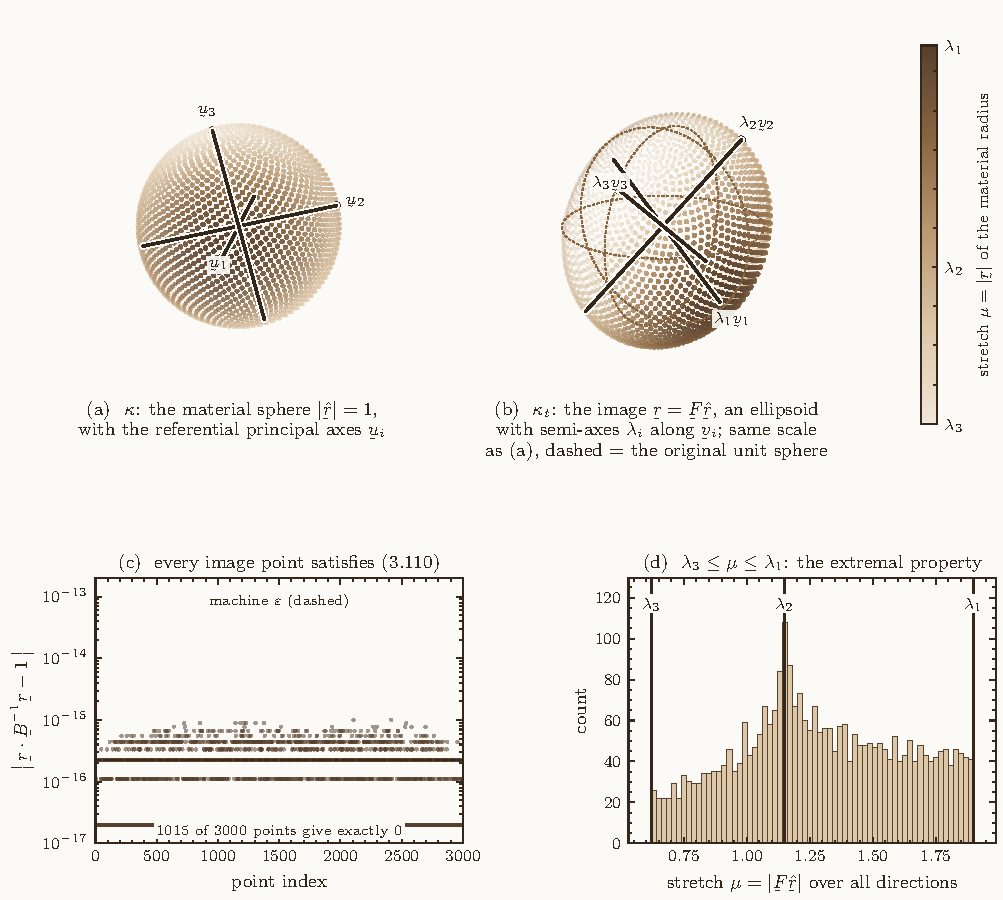
\includegraphics[width=\textwidth]{sphere_to_ellipsoid.pdf}
\caption{Property (c) tested numerically, by the script
\texttt{sphere\_to\_ellipsoid.py}. Three thousand points are spread over
the unit material sphere by a golden-angle spiral and pushed forward by
one fixed $\bF=\bR\bU$ with principal stretches
$\lambda=(1.90,\,1.15,\,0.62)$ and $J=\det\bF=1.3547$. Every marker in
the figure is an individual vector point, not a raster image.
(a) the sphere in $\kappa$, each point shaded by the stretch that material
radius will undergo, with the referential principal axes $\bu_{i}$.
(b) the image in $\kappa_{t}$, at the same scale, with the original sphere
retained as dashed great circles for comparison; the point cloud lies on
an ellipsoid with semi-axes $\lambda_{i}$ along $\bv_{i}$, exactly as
\eqr{3.112} asserts.
(c) the residual $|\ip{\br}{\bB^{-1}\br}-1|$ of \eqr{3.110} for every one of
the three thousand image points, at or below machine precision throughout,
with $1015$ of them exactly zero.
(d) the distribution of the stretch $\mu=|\bF\hat\br|$ over all directions,
confined between $\lambda_{3}$ and $\lambda_{1}$ as the extremal property
\eqr{3.26} requires, with $\lambda_{2}$ falling inside.}
\label{fig:numellipsoid}
\end{figure}

\begin{remark}[what the numerical test in Figure~\ref{fig:numellipsoid}
actually checks]\label{rem:numcheck}
Panels (c) and (d) are the substance; (a) and (b) only make the result
visible. Four separate predictions of the text are tested, and all four
hold to about $10^{-15}$:

$\bullet$\ \ \eqr{3.110}, $\ip{\br}{\bB^{-1}\br}=1$, panel (c);

$\bullet$\ \ \eqr{3.112}, $\sum_{i}(r_{i}/\lambda_{i})^{2}=1$ with
$r_{i}=\ip{\bv_{i}}{\br}$, the same statement resolved on the principal
frame;

$\bullet$\ \ \eqr{3.17}, $\lambda_{1}\lambda_{2}\lambda_{3}=J$, so that the
ellipsoid volume $\tfrac43\pi\lambda_{1}\lambda_{2}\lambda_{3}$ is exactly
$J$ times the sphere volume;

$\bullet$\ \ \eqr{3.44}, $\bF\bu_{i}=\lambda_{i}\bv_{i}$, so the axes really
are the images of the referential principal directions.

One check is deliberately \emph{not} at machine precision, and it should
not be. The semi-axis lengths measured from the cloud, $\max_{\text{cloud}}
|\ip{\bv_{i}}{\br}|$, come out about $4\times10^{-4}$ below $\lambda_{i}$.
That is not an error in \eqr{3.112} but a consequence of sampling: with
finitely many points, none lands exactly on an axis tip, so the measured
semi-axis always undershoots. The script confirms the diagnosis by
refining the cloud, and the discrepancy falls from $3.3\times10^{-4}$ at
$N=3000$ to $1.8\times10^{-5}$ at $N=30\,000$ and
$1.5\times10^{-6}$ at $N=300\,000$, that is like $1/N$.
Distinguishing a discretisation error from a genuine one is the whole
skill of testing a formula numerically.

The script also runs the test backwards. It builds $\bF$ from a chosen
$\bR$ and $\bU$, then throws them away and recovers them from $\bF$ alone
by Theorem~\ref{thm:Uclosed}, that is by the closed form
$\bU=(-\bC^{2}+(i_{1}^{2}-i_{2})\bC+i_{1}i_{3}\hI)/(i_{1}i_{2}-i_{3})$ with
$i_{1}$ from the quartic $(\ast_{2})$. The recovered $\bU$ and $\bR$ agree
with the originals to $5\times10^{-15}$, $\bR^{t}\bR=\hI$ and
$\det\bR=1$ hold to the same order, and both $\bF=\bR\bU$ and
$\bF=\bV\bR$ are reproduced. So the closed form of \S3.4 is not merely
derived, it is executed.
\end{remark}

\begin{remark}[the ellipsoid is the picture of the polar decomposition]
\label{rem:ellipsoid}
Property (c) is $\bF=\bV\bR$ drawn. The rotation $\bR$ takes the unit
sphere to the unit sphere, since it preserves lengths, and therefore
contributes nothing to the shape; all of the shape comes from $\bV$, which
stretches the sphere by $\lambda_{i}$ along $\bv_{i}$. Conversely, if one
measures the ellipsoid in $\kappa_{t}$ one recovers $\bV$ completely and
$\bR$ not at all. This is exactly the sense in which the ellipsoid, and
not $\bF$, is what the material experiences.
\end{remark}

%=======================================================================
\section{Rigid-body motions}\label{sec:rigid}
%=======================================================================

\subsection*{Where we are and why this section closes the chapter}

The chapter opened with a promise: separate the part of $\bF$ that a
material feels from the part it does not. \S3.4 delivered the separation,
$\bF=\bR\bU$, and asserted that $\bR$ is the part that costs nothing. That
assertion has not yet been proved. This section proves it, in the sharpest
possible form: the motions in which \emph{nothing at all} happens to the
material are exactly the motions with $\bU=\hI$, that is exactly the
motions in which $\bF$ is a rotation. Once that is established, the case
for writing constitutive laws in terms of $\bC$ rather than $\bF$ is
complete, and the chapter is finished.

The logic runs the opposite way from \S3.6. There we assumed something
about $\bF$ and deduced geometry; here we assume something purely
geometric, that distances are preserved, and deduce what $\bF$ must be.

A motion is \emph{rigid} if it preserves the distance between every pair of
material points, i.e.\ if
$|\bchi_{\kappa}(\bY,t)-\bchi_{\kappa}(\bX,t)|=|\bY-\bX|$, or, squaring to
remove the square root,
\begin{equation}
   \ip{[\bchi_{\kappa}(\bY,t)-\bchi_{\kappa}(\bX,t)]}
      {[\bchi_{\kappa}(\bY,t)-\bchi_{\kappa}(\bX,t)]}
   =\ip{(\bY-\bX)}{(\bY-\bX)}
   \tag{3.113}\label{eq:3.113}
\end{equation}
for all $\bX,\bY$. Squaring is not cosmetic: the square root in the
definition is awkward to differentiate at $\bY=\bX$, whereas the quadratic
form on each side of \eqr{3.113} is a polynomial and differentiates cleanly.

\emph{The plan.} We have a functional equation, \eqr{3.113}, holding for all
pairs of points, and we want a statement about $\bF$. The route is to
differentiate twice, once with respect to $\bY$ and once with respect to
$\bX$, because each differentiation converts a difference of positions
into an $\bF$, by the definition $\dl\bchi_{\kappa}=\bF\,\dl\bX$. Two
differentiations therefore produce a relation between two $\bF$'s, and that
relation will turn out to say both that $\bF$ is orthogonal and that it
does not vary.

\emph{First differentiation.} Differentiate \eqr{3.113}. Both sides have the
form $\ip\ba\ba$, whose differential is
$\dl(\ip\ba\ba)=\ip{\dl\ba}{\ba}+\ip{\ba}{\dl\ba}=2\ip{\ba}{\dl\ba}$, the
two terms being equal because the dot product is symmetric. The factor $2$
appears on both sides and cancels, leaving
\begin{equation}
   \ip{[\bchi_{\kappa}(\bY,t)-\bchi_{\kappa}(\bX,t)]}
      {\dl[\bchi_{\kappa}(\bY,t)-\bchi_{\kappa}(\bX,t)]}
   =\ip{(\bY-\bX)}{\dl(\bY-\bX)},
   \tag{3.114}\label{eq:3.114}
\end{equation}
in which the derivative may be taken with respect to $\bX$ or to $\bY$; we
choose $\bY$ first.

So fix $\bX$, which makes $\bchi_{\kappa}(\bX,t)$ a constant vector, and
let $\bY$ vary. Then
\[
   \dl\big[\bchi_{\kappa}(\bY,t)-\bchi_{\kappa}(\bX,t)\big]
   =\dl\bchi_{\kappa}(\bY,t)-\bze=\bF(\bY,t)\,\dl\bY,
   \qquad
   \dl(\bY-\bX)=\dl\bY ,
\]
the first by the definition \eqr{2.34} of the deformation gradient at the
point $\bY$. Substituting into \eqr{3.114},
\begin{equation}
   \ip{[\bchi_{\kappa}(\bY,t)-\bchi_{\kappa}(\bX,t)]}{\bF(\bY,t)\dl\bY}
   =\ip{(\bY-\bX)}{\dl\bY}
   \tag{3.115}\label{eq:3.115}
\end{equation}
for all $\dl\bY$. Move $\bF$ to the other factor by the definition of the
transpose, $\ip{\ba}{\bF\bb}=\ip{\bF^{t}\ba}{\bb}$, and collect:
\[
   \ip{\Big(\bF^{t}(\bY,t)\big[\bchi_{\kappa}(\bY,t)
      -\bchi_{\kappa}(\bX,t)\big]-(\bY-\bX)\Big)}{\dl\bY}=0
   \quad\text{for all }\dl\bY .
\]
A vector orthogonal to every vector is $\bze$, so the bracket vanishes:
\begin{equation}
   \bF^{t}(\bY,t)\big[\bchi_{\kappa}(\bY,t)-\bchi_{\kappa}(\bX,t)\big]
   =\bY-\bX .
   \tag{3.116}\label{eq:3.116}
\end{equation}

\emph{Second differentiation.} Now reverse the roles: fix $\bY$, so that
$\bF^{t}(\bY,t)$ and $\bchi_{\kappa}(\bY,t)$ are both constant, and
differentiate \eqr{3.116} with respect to $\bX$. On the left, the only
$\bX$-dependent piece is $-\bchi_{\kappa}(\bX,t)$, whose differential is
$-\bF(\bX,t)\dl\bX$, and the constant tensor $\bF^{t}(\bY,t)$ multiplies
it. On the right, the only $\bX$-dependent piece is $-\bX$. Hence
\[
   -\bF^{t}(\bY,t)\bF(\bX,t)\,\dl\bX=-\dl\bX
   \qquad\text{for all }\dl\bX ,
\]
and cancelling the minus signs and using once more that two tensors
agreeing on every vector are equal,
\begin{equation}
   \bF^{t}(\bY,t)\bF(\bX,t)=\hI\qquad\text{for all }\bX,\bY\in\kappa .
   \tag{3.117}\label{eq:3.117}
\end{equation}
Putting $\bY=\bX$,
\begin{equation}
   \bF^{t}(\bX,t)\bF(\bX,t)=\hI\qquad\text{for all }\bX\in\kappa ,
   \tag{3.118}\label{eq:3.118}
\end{equation}
so $\bF(\bX,t)$ is orthogonal at every $\bX$ and $\bF^{t}=\bF^{-1}$.
Substituting this back into \eqr{3.117} gives
$\bF^{-1}(\bY,t)\bF(\bX,t)=\hI$, i.e.
\begin{equation}
   \bF(\bY,t)=\bF(\bX,t)\qquad\text{for all }\bX,\bY\in\kappa ,
   \tag{3.119}\label{eq:3.119}
\end{equation}
so $\bF$ does not depend on $\bX$ at all:
\begin{equation}
   \bF(\bX,t)=\bQ(t),
   \tag{3.120}\label{eq:3.120}
\end{equation}
a uniform orthogonal tensor, and a rotation if $\kappa$ is occupiable, by
\eqr{2.50}. Rigid motions are therefore homogeneous, and \eqr{3.100} gives
\begin{equation}
   \bx=\bchi_{\kappa}(\bX,t)=\bQ(t)\bX+\bc(t).
   \tag{3.121}\label{eq:3.121}
\end{equation}
Conversely, substituting \eqr{3.121} into the left side of \eqr{3.113} gives
$\ip{\bQ(\bY-\bX)}{\bQ(\bY-\bX)}=\ip{(\bY-\bX)}{\bQ^{t}\bQ(\bY-\bX)}
=\ip{(\bY-\bX)}{(\bY-\bX)}$, so \eqr{3.121} is necessary \emph{and}
sufficient for rigidity.

The polar decomposition is trivial in this case:
\begin{equation}
   \bR=\bQ,\qquad \bU=\hI,\qquad \bV=\I,
   \tag{3.122}\label{eq:3.122}
\end{equation}
and of course $\bC=\hI$ and $\bB=\I$. Uniqueness makes this immediate:
$\bQ=\bQ\hI$ is a factorisation of the required type, hence \emph{the}
one.

\bookfig{7}\begin{figure}[htbp]\centering
\begin{tikzpicture}[scale=1.0,
  vec/.style={-{Stealth[length=2.2mm]},thick},
  lbl/.style={fill=white,inner sep=1pt,font=\small}]
\begin{scope}
\blob{thick}
\coordinate (X) at (-0.35,0.30);
\coordinate (Y) at (0.85,-0.45);
\fill (X) circle (1pt); \fill (Y) circle (1pt);
\node[lbl,left] at (X) {$\bX$}; \node[lbl,right] at (Y) {$\bY$};
\draw[thick] (X)--(Y);
\node[lbl,font=\small] at (0.32,0.05) {$\ell$};
\node[lbl] at (0,-1.65) {$\kappa$};
\end{scope}
\draw[-{Stealth[length=2.6mm]},thick,gray!70] (2.1,0)--(3.5,0);
\node[lbl,above,text=gray!85] at (2.8,0.05) {$\bchi_{\kappa}$};
\begin{scope}[xshift=6.1cm,rotate=-34]
\blob{thick}
\coordinate (X2) at (-0.35,0.30);
\coordinate (Y2) at (0.85,-0.45);
\fill (X2) circle (1pt); \fill (Y2) circle (1pt);
\draw[thick] (X2)--(Y2);
\end{scope}
\node[lbl] at (6.1,-1.65) {$\kappa_{t}$};
\node[lbl,font=\small] at (6.5,0.55) {same $\ell$};
\end{tikzpicture}
\caption{Rigid-body motion. Every material distance is
preserved, so the body may translate and turn but cannot change shape. The
computation \eqr{3.113} to \eqr{3.120} shows that this forces $\bF$ to be a
uniform rotation, hence $\bU=\hI$ and $\bC=\hI$: no stretching anywhere.}
\label{fig:37}
\end{figure}

\begin{remark}[why this is the theorem the whole chapter was for]
\label{rem:rigidwhy}
\eqr{3.122} says: rigid motion $\iff$ $\bU=\hI$ $\iff$ $\bC=\hI$ $\iff$
$\bE=\hOb$. The strain tensors vanish exactly on motions in which nothing
happens to the material. That is the property one demands of a strain
measure, and it is why $\bE=\tfrac12(\bC-\hI)$ was defined with the $\hI$
subtracted. Note what is \emph{not} true: $\bF=\I$ is not the condition
for rigidity, since $\bF=\bQ(t)$ with $\bQ\neq\I$ is rigid too. A
constitutive law written in terms of $\bF$ would therefore assign energy
to a body that is merely being carried around; a law written in terms of
$\bC$ cannot. This is the whole reason for \S3.4.
\end{remark}

%=======================================================================
\setcounter{problemenv}{0}
\section{Problems}\label{sec:problems:c3}
%=======================================================================

All nine problems of the chapter are solved below in the book's order and
notation. They fall into three groups, and it helps to know which is which
before starting.

\emph{Problems 1, 4, 5, 6 are further worked deformations}, in the style of
\S3.5: write down $\bx$, differentiate, read off $\bF$, then extract what
is asked. The recipe of \S3.5 applies verbatim, and rules (R1)--(R4) are
used throughout. Problem 1 adds area change through Piola--Nanson,
Problem 4 is spherically symmetric rather than cylindrical, Problem 5 is a
fourth shear, and Problem 6 is bending.

\emph{Problems 2, 7, 8 are algebra}, filling gaps that \S\S3.1--3.4 left
open: that products of rotations are rotations, which was used at \eqr{3.95};
that the invariants are the elementary symmetric functions of the
principal values, which was used at \eqr{3.17} and in
Remark~\ref{rem:invgeom}; and the Cayley--Hamilton theorem, which is what
makes Theorem~\ref{thm:Uclosed} and Problem 9 possible.

\emph{Problems 3 and 9 are the pay-off.} Problem 3 completes torsion, and
Problem 9 produces the closed form for $\bU$ that removes eigenvectors from
the subject entirely, in two dimensions; Theorem~\ref{thm:Uclosed} did the
same in three.

%-----------------------------------------------------------------------
\begin{problem}[Triaxial stretch: area change and normals]
Consider the deformation $x_{1}=\lambda_{1}X_{1}$,
$x_{2}=\lambda_{2}X_{2}$, $x_{3}=\lambda_{3}X_{3}$ with constant
$\lambda_{i}$ and $\{\be_{i}\}=\{\bE_{A}\}$.
(a) Obtain $\bF$ and state a restriction on the $\lambda_{i}$ for the
deformation to be physically possible.
(b) With $\lambda_{3}=\lambda_{2}$ and the deformation isochoric, consider
a plane material surface in $\kappa$ whose unit normal is inclined at
angle $\phi$ to the $1$-axis. Find, in terms of $\lambda_{1}$ and $\phi$,
the ratio of its deformed area to its undeformed area.
(c) What is the unit normal to that surface after deformation?
\end{problem}

\begin{solution}
\textbf{(a)} Differentiating the three relations at fixed $t$,
$\dl x_{i}=\lambda_{i}\dl X_{i}$ (no sum), and
$\dl X_{A}=\ip{\hbE_{A}}{\dl\bX}$, so
\[
   \dl\bx=\dl x_{i}\be_{i}
   =\sum_{A=1}^{3}\lambda_{A}\,\be_{A}\,(\ip{\hbE_{A}}{\dl\bX})
   =\Big(\sum_{A=1}^{3}\lambda_{A}\,\be_{A}\otimes\hbE_{A}\Big)\dl\bX ,
\]
whence
\[
   \bF=\lambda_{1}\,\be_{1}\otimes\hbE_{1}
      +\lambda_{2}\,\be_{2}\otimes\hbE_{2}
      +\lambda_{3}\,\be_{3}\otimes\hbE_{3}.
\]
This is already in the form \eqr{3.43} with orthonormal frames on both
sides, so if the $\lambda_{A}$ are positive they \emph{are} the principal
stretches, $\bU=\sum\lambda_{A}\hbE_{A}\otimes\hbE_{A}$,
$\bV=\sum\lambda_{A}\be_{A}\otimes\be_{A}$ and $\bR=\shift$. The Jacobian
is
obtained as follows. First the images of the referential frame, each by
(R1) applied to the three dyads:
\[
   \bF\hbE_{1}=\lambda_{1}\be_{1},\qquad
   \bF\hbE_{2}=\lambda_{2}\be_{2},\qquad
   \bF\hbE_{3}=\lambda_{3}\be_{3},
\]
since for instance $\bF\hbE_{1}=\lambda_{1}(\ip{\hbE_{1}}{\hbE_{1}})\be_{1}
+\lambda_{2}(\ip{\hbE_{2}}{\hbE_{1}})\be_{2}
+\lambda_{3}(\ip{\hbE_{3}}{\hbE_{1}})\be_{3}
=\lambda_{1}\be_{1}$. Then rule (R4), with the denominator
$\tbox{\hbE_{1}}{\hbE_{2}}{\hbE_{3}}=1$ by Lemma~\ref{lem:boxortho} and
the scalars taken out one slot at a time by (R3):
\[
\begin{aligned}
   J=\det\bF
   &=\frac{\tbox{\bF\hbE_{1}}{\bF\hbE_{2}}{\bF\hbE_{3}}}
          {\tbox{\hbE_{1}}{\hbE_{2}}{\hbE_{3}}}
    =\frac{\tbox{\lambda_{1}\be_{1}}{\lambda_{2}\be_{2}}
                {\lambda_{3}\be_{3}}}{1}\\
   &=\lambda_{1}\lambda_{2}\lambda_{3}\,
     \tbox{\be_{1}}{\be_{2}}{\be_{3}}
    =\lambda_{1}\lambda_{2}\lambda_{3}\cdot1
    =\lambda_{1}\lambda_{2}\lambda_{3}.
\end{aligned}
\]
\subsubsection*{The restriction on the $\lambda_{A}$}

Two requirements, excluding different things.

\emph{Invertibility.} If $\lambda_{1}=0$ then $\hbE_{1}$ and $2\hbE_{1}$
both map to $\bze$, contradicting \eqr{2.1}. So $\lambda_{A}\neq0$ and
$J\neq0$.

\emph{Sign.} Along a motion, $\bF(t_{0})=\shift$ by \eqr{2.79}, so
$J(t_{0})=1>0$. Now $J(t)$ is continuous and never zero, so by the
intermediate value theorem it cannot change sign. Hence
\[
   \boxed{\ J=\lambda_{1}\lambda_{2}\lambda_{3}>0\ }
\]

This is weaker than $\lambda_{A}>0$. Assuming no signs,
\[
   \bC=\sum_{A}\lambda_{A}^{2}\,\hbE_{A}\otimes\hbE_{A},
   \qquad
   \bU=\sqrt{\bC}=\sum_{A}|\lambda_{A}|\,\hbE_{A}\otimes\hbE_{A},
\]
the positive root by Theorem~\ref{thm:sqrt}, and with
$s_{A}=\operatorname{sgn}\lambda_{A}$,
\[
\begin{aligned}
   \bR&=\bF\bU^{-1}
   =\sum_{A}\frac{\lambda_{A}}{|\lambda_{A}|}\,\be_{A}\otimes\hbE_{A}
   =\sum_{A}s_{A}\,\be_{A}\otimes\hbE_{A},\\
   \det\bR&=s_{1}s_{2}s_{3}=\operatorname{sgn}J .
\end{aligned}
\]
So $\bR$ is a rotation exactly when $J>0$. The four sign patterns:
\[
\begin{array}{cccl}
   (s_{A}) & J & \bR & \\[1mm]
   (+,+,+) & >0 & \shift & \text{pure stretch}\\
   (-,+,+) & <0 & \operatorname{diag}(-1,1,1) & \text{mirror, excluded}\\
   (-,-,+) & >0 & \operatorname{diag}(-1,-1,1) &
     \text{half turn about }\be_{3},\ \text{admissible}\\
   (-,-,-) & <0 & -\shift & \text{inversion, excluded}
\end{array}
\]
The stretches are $|\lambda_{A}|$, not $\lambda_{A}$. Parts (b) and (c)
speak of stretches, so take $\lambda_{A}>0$ below.


\begin{figure}[htbp]\centering
\renewcommand{\thefigure}{E}
\begin{tikzpicture}[x={(-0.50cm,-0.36cm)},y={(1cm,-0.20cm)},z={(0cm,1cm)},
  scale=1.22,
  vec/.style={-{Stealth[length=2.4mm]},thick},
  lbl/.style={fill=white,inner sep=1pt,font=\small}]
% ---------------- reference cube ----------------
\begin{scope}
\fill[gray!10] (0,0,0)--(1,0,0)--(1,1,0)--(0,1,0)--cycle;
\fill[gray!16] (0,0,0)--(1,0,0)--(1,0,1)--(0,0,1)--cycle;
\fill[gray!8]  (0,0,0)--(0,1,0)--(0,1,1)--(0,0,1)--cycle;
\draw[thin,gray!70] (0,0,0)--(1,0,0)--(1,1,0)--(0,1,0)--cycle;
\draw[thin,gray!70] (0,0,1)--(1,0,1)--(1,1,1)--(0,1,1)--cycle;
\foreach \a/\b in {0/0,1/0,1/1,0/1}
  \draw[thin,gray!70] (\a,\b,0)--(\a,\b,1);
\draw[vec] (0,0,0)--(1.55,0,0); \node[lbl] at (1.80,0,0) {$\hbE_{1}$};
\draw[vec] (0,0,0)--(0,1.55,0); \node[lbl] at (0,1.80,0) {$\hbE_{2}$};
\draw[vec] (0,0,0)--(0,0,1.55); \node[lbl] at (0,0,1.80) {$\hbE_{3}$};
\node[font=\small,align=center] at (0.5,0.5,-1.32)
  {$\kappa$: the unit cube,\\
   $\tbox{\hbE_{1}}{\hbE_{2}}{\hbE_{3}}=+1$};
\end{scope}
% ---------------- two negative: admissible ----------------
\begin{scope}[yshift=3.6cm]
\fill[gray!10] (0,0,0)--(-1.5,0,0)--(-1.5,-1.1,0)--(0,-1.1,0)--cycle;
\fill[gray!16] (0,0,0)--(-1.5,0,0)--(-1.5,0,0.7)--(0,0,0.7)--cycle;
\draw[thin,gray!70] (0,0,0)--(-1.5,0,0)--(-1.5,-1.1,0)--(0,-1.1,0)--cycle;
\draw[thin,gray!70] (0,0,0.7)--(-1.5,0,0.7)--(-1.5,-1.1,0.7)--(0,-1.1,0.7)
  --cycle;
\foreach \a/\b in {0/0,-1.5/0,-1.5/-1.1,0/-1.1}
  \draw[thin,gray!70] (\a,\b,0)--(\a,\b,0.7);
\draw[vec] (0,0,0)--(-2.0,0,0); \node[lbl] at (-2.35,0,0) {$\lambda_{1}\be_{1}$};
\draw[vec] (0,0,0)--(0,-1.6,0); \node[lbl] at (0,-1.95,0) {$\lambda_{2}\be_{2}$};
\draw[vec] (0,0,0)--(0,0,1.2); \node[lbl] at (0,0,1.45) {$\lambda_{3}\be_{3}$};
\node[font=\small,align=center] at (-0.75,-0.55,-1.32)
  {$\lambda=(-1.5,\,-1.1,\,0.7)$:\ \
   $\tbox{\bF\hbE_{1}}{\bF\hbE_{2}}{\bF\hbE_{3}}=+1.155$\\
   still right handed; $\bR$ is the half turn about $\be_{3}$
   \ \checkmark};
\end{scope}
% ---------------- one negative: inadmissible ----------------
\begin{scope}[yshift=7.6cm]
\fill[gray!10] (0,0,0)--(-1.5,0,0)--(-1.5,1.1,0)--(0,1.1,0)--cycle;
\fill[gray!16] (0,0,0)--(-1.5,0,0)--(-1.5,0,0.7)--(0,0,0.7)--cycle;
\draw[thin,gray!70] (0,0,0)--(-1.5,0,0)--(-1.5,1.1,0)--(0,1.1,0)--cycle;
\draw[thin,gray!70] (0,0,0.7)--(-1.5,0,0.7)--(-1.5,1.1,0.7)--(0,1.1,0.7)
  --cycle;
\foreach \a/\b in {0/0,-1.5/0,-1.5/1.1,0/1.1}
  \draw[thin,gray!70] (\a,\b,0)--(\a,\b,0.7);
\draw[vec] (0,0,0)--(-2.0,0,0); \node[lbl] at (-2.35,0,0) {$\lambda_{1}\be_{1}$};
\draw[vec] (0,0,0)--(0,1.6,0); \node[lbl] at (0,1.95,0) {$\lambda_{2}\be_{2}$};
\draw[vec] (0,0,0)--(0,0,1.2); \node[lbl] at (0,0,1.45) {$\lambda_{3}\be_{3}$};
\node[font=\small,align=center] at (-0.75,0.55,-1.32)
  {$\lambda=(-1.5,\,1.1,\,0.7)$:\ \
   $\tbox{\bF\hbE_{1}}{\bF\hbE_{2}}{\bF\hbE_{3}}=-1.155$\\
   now left handed; $\bR$ is a mirror \ $\times$};
\end{scope}
\end{tikzpicture}
\caption{Why the restriction is $\lambda_{1}\lambda_{2}\lambda_{3}>0$ and
not $\lambda_{A}>0$. Bottom, the reference cube with its right-handed
frame. Middle, two of the $\lambda$'s negative: the frame is turned
through $\pi$ about $\be_{3}$ but is still right handed, the box product
is still positive, and the deformation is a genuine one, a pure stretch
followed by a half turn. Top, one $\lambda$ negative: the frame has become
left handed, the box product is negative, and $\bR$ is a mirror. No
continuous motion starting from $\bF=\shift$ can reach it, because $J$
would have to pass through zero and $\bF$ would cease to be invertible at
that instant.}
\label{fig:signs}
\end{figure}

\textbf{(b)} Isochoric with $\lambda_{3}=\lambda_{2}$ means
$\lambda_{1}\lambda_{2}^{2}=1$, so
\[
   \lambda_{2}=\lambda_{3}=\lambda_{1}^{-1/2}.
\]
Take the normal in the $(1,2)$ plane without loss of generality, since the
$2$ and $3$ directions are now equivalent:
\[
   \bN=\cos\phi\,\hbE_{1}+\sin\phi\,\hbE_{2}.
\]
The Piola--Nanson formula \eqr{2.54} with \eqr{2.55} gives
$\bn\,\dl a=\bF^{*}\bN\,\dl A$ and $\bF^{*}=J\bF^{-t}=\bF^{-t}$ since
$J=1$. From the dyadic form of $\bF$,
\[
   \bF^{-1}=\sum_{A}\lambda_{A}^{-1}\,\hbE_{A}\otimes\be_{A},
   \qquad
   \bF^{-t}=\sum_{A}\lambda_{A}^{-1}\,\be_{A}\otimes\hbE_{A},
\]
the first because
\[
   \Big(\sum_{A}\lambda_{A}^{-1}\hbE_{A}\otimes\be_{A}\Big)
   \Big(\sum_{B}\lambda_{B}\be_{B}\otimes\hbE_{B}\Big)
   =\sum_{A,B}\lambda_{A}^{-1}\lambda_{B}\dd_{AB}
    \,\hbE_{A}\otimes\hbE_{B}=\hI .
\]
Therefore
\[
   \bF^{*}\bN=\lambda_{1}^{-1}\cos\phi\,\be_{1}
             +\lambda_{2}^{-1}\sin\phi\,\be_{2},
\]
and taking the length of both sides of $\bn\,\dl a=\bF^{*}\bN\,\dl A$,
with $|\bn|=1$,
\[
   \frac{\dl a}{\dl A}=|\bF^{*}\bN|
   =\sqrt{\lambda_{1}^{-2}\cos^{2}\phi+\lambda_{2}^{-2}\sin^{2}\phi}
   =\boxed{\ \sqrt{\lambda_{1}^{-2}\cos^{2}\phi+\lambda_{1}\sin^{2}\phi}\ }
\]
where $\lambda_{2}^{-2}=(\lambda_{1}^{-1/2})^{-2}=\lambda_{1}$ was used.

Checks. At $\lambda_{1}=1$ the deformation is the identity and the formula
gives $\sqrt{\cos^{2}\phi+\sin^{2}\phi}=1$. At $\phi=0$ the surface is
normal to the stretching axis and the ratio is $\lambda_{1}^{-1}$, which
is right: that face has area $\lambda_{2}\lambda_{3}=\lambda_{1}^{-1}$
times its original. At $\phi=\pi/2$ the ratio is $\lambda_{1}^{1/2}
=\lambda_{1}\lambda_{3}=\lambda_{1}\lambda_{1}^{-1/2}$, also right.

\textbf{(c)} Dividing $\bF^{*}\bN$ by its length,
\[
   \bn=\frac{\lambda_{1}^{-1}\cos\phi\,\be_{1}
             +\lambda_{1}^{1/2}\sin\phi\,\be_{2}}
            {\sqrt{\lambda_{1}^{-2}\cos^{2}\phi+\lambda_{1}\sin^{2}\phi}},
\]
using $\lambda_{2}^{-1}=\lambda_{1}^{1/2}$. Equivalently, the deformed
normal makes an angle $\psi$ with the $1$-axis given by
\[
   \tan\psi=\lambda_{1}^{3/2}\tan\phi .
\]
Note that the normal does \emph{not} rotate the way the material does: for
$\lambda_{1}>1$ it turns \emph{away} from the stretching axis, because
$\bF^{-t}$, not $\bF$, transports normals. This is the standard trap that
Piola--Nanson exists to avoid.
\end{solution}

%-----------------------------------------------------------------------
\begin{problem}[Products of orthogonal tensors]
Prove that the product of two orthogonal tensors is orthogonal, and that
the product of two rotations is a rotation.
\end{problem}

\begin{solution}
Let $\bQ_{1},\bQ_{2}$ be orthogonal, meaning $\bQ_{k}^{t}\bQ_{k}=\I$.
Using $(\bA\bB)^{t}=\bB^{t}\bA^{t}$ from Problem 20 of Chapter 1 and
associativity,
\[
   (\bQ_{1}\bQ_{2})^{t}(\bQ_{1}\bQ_{2})
   =\bQ_{2}^{t}\bQ_{1}^{t}\bQ_{1}\bQ_{2}
   =\bQ_{2}^{t}\,\I\,\bQ_{2}
   =\bQ_{2}^{t}\bQ_{2}=\I ,
\]
so $\bQ_{1}\bQ_{2}$ is orthogonal.

Two gaps to close. First, $\bQ^{t}\bQ=\I$ implies $\bQ\bQ^{t}=\I$: if
$\bQ\ba=\bze$ then $\ba=\bQ^{t}\bQ\ba=\bze$, so $\bQ$ is injective, hence
bijective in finite dimensions, hence $\bQ^{-1}=\bQ^{t}$ and
$\bQ\bQ^{t}=\I$. Second, $\det\bQ^{t}\det\bQ=\det\I=1$ with
$\det\bQ^{t}=\det\bQ$ gives $(\det\bQ)^{2}=1$, so $\det\bQ=\pm1$.

\emph{What orthogonality means.} The three statements
\[
   \bQ^{t}\bQ=\I,
   \qquad
   \ip{\bQ\ba}{\bQ\bb}=\ip\ba\bb\ \ \forall\ba,\bb,
   \qquad
   |\bQ\ba|=|\ba|\ \ \forall\ba
\]
are equivalent. The first gives the second by
$\ip{\bQ\ba}{\bQ\bb}=\ip{\ba}{\bQ^{t}\bQ\bb}=\ip\ba\bb$; the second gives
the third at $\bb=\ba$; and the third gives the second by polarisation,
\[
   \ip\ba\bb=\tfrac12\big(|\ba+\bb|^{2}-|\ba|^{2}-|\bb|^{2}\big),
\]
each term of which is preserved. The second then gives the first, since
$\ip{\ba}{(\bQ^{t}\bQ-\I)\bb}=0$ for all $\ba,\bb$. So a product of
orthogonal tensors is orthogonal for a reason needing no algebra: doing
two length-preserving maps in succession preserves lengths.

A \emph{rotation} is an orthogonal tensor with $\det=+1$. By Problem 21(b)
of Chapter 1,
\[
   \det(\bQ_{1}\bQ_{2})=(\det\bQ_{1})(\det\bQ_{2})=(+1)(+1)=+1 ,
\]
so a product of rotations is a rotation.

The version actually used at \eqr{3.95} is the two-point one: if
$\bQ_{1}\in\Orth(\hVt,\Vt)$ and $\bQ_{2}\in\Orth(\hVt,\hVt)$ then
$\bQ_{1}\bQ_{2}\in\Orth(\hVt,\Vt)$. The computation is identical, the
only change being that $\bQ_{2}^{t}\bQ_{2}=\hI$ and
$\bQ_{1}^{t}\bQ_{1}=\hI$, so the chain reads
$(\bQ_{1}\bQ_{2})^{t}(\bQ_{1}\bQ_{2})=\bQ_{2}^{t}\hI\bQ_{2}=\hI$; and
the determinant statement uses the extension recorded in
Remark~\ref{rem:detext}.
\end{solution}

%-----------------------------------------------------------------------
\begin{problem}[Torsion: Cauchy--Green tensors and principal stretches]
Evaluate the left and right Cauchy--Green tensors for the torsion problem.
Find the principal stretches in terms of the twist $\tau$. Verify that
azimuthal shear and torsion are isochoric.
\end{problem}

\begin{solution}
From \eqr{3.88} and \eqr{3.97}, $\bF=\bQ\hat\bG=\bG\bQ$ with
\[
   \hat\bG=\hI+\gamma\,\hETh\otimes\hbE_{3},\qquad
   \bG=\I+\gamma\,\bet\otimes\be_{3},\qquad \gamma=\gamma(R)=R\tau .
\]
Since $\bQ^{t}\bQ=\hI$ and $\bQ\bQ^{t}=\I$, exactly as in \eqr{3.91},
\[
   \bC=\hat\bG^{t}\bQ^{t}\bQ\hat\bG=\hat\bG^{t}\hat\bG,
   \qquad
   \bB=\bG\bQ\bQ^{t}\bG^{t}=\bG\bG^{t}.
\]
With $\hat\bG^{t}=\hI+\gamma\,\hbE_{3}\otimes\hETh$,
\[
\begin{aligned}
   \bC&=(\hI+\gamma\hbE_{3}\otimes\hETh)(\hI+\gamma\hETh\otimes\hbE_{3})\\
   &=\hI+\gamma\,\hETh\otimes\hbE_{3}+\gamma\,\hbE_{3}\otimes\hETh
     +\gamma^{2}(\ip{\hETh}{\hETh})\,\hbE_{3}\otimes\hbE_{3}\\
   &=\hI+\gamma\big[\hETh(\Theta)\otimes\hbE_{3}
      +\hbE_{3}\otimes\hETh(\Theta)\big]
      +\gamma^{2}\,\hbE_{3}\otimes\hbE_{3},
\end{aligned}
\]
and in the same way
\[
   \bB=\I+\gamma\big[\bet(\theta)\otimes\be_{3}
      +\be_{3}\otimes\bet(\theta)\big]
      +\gamma^{2}\,\bet(\theta)\otimes\bet(\theta).
\]
Note again the shift of the squared term from $\hbE_{3}$ in $\bC$ to
$\bet$ in $\bB$, exactly as in Remark~\ref{rem:CnotB}.

\emph{Principal stretches.} In the orthonormal basis
$\{\hER,\hETh,\hbE_{3}\}$ the matrix of $\bC$ is
\[
   (C_{AB})=\begin{pmatrix}1&0&0\\ 0&1&\gamma\\ 0&\gamma&1+\gamma^{2}
   \end{pmatrix},
\]
which is \eqr{3.55} with the roles of the axes permuted: the shear acts on
the pair $(\hETh,\hbE_{3})$ and $\hER$ is inert. Hence one principal
stretch is $1$, with principal direction $\hER$, and the other two solve
the same quadratic as before. Reading \eqr{3.60} with $\gamma=R\tau$,
\[
   \boxed{\ \lambda_{1}=\tfrac12\big(R\tau+\sqrt{4+R^{2}\tau^{2}}\big),
   \qquad \lambda_{2}=\lambda_{1}^{-1},\qquad \lambda_{3}=1 .\ }
\]
The stretches depend on $R$: fibres near the axis are barely deformed,
fibres near the outer surface most. At $R=0$ all three are $1$, which is
right, since the axis of a twisted bar is not deformed at all.

\emph{Isochoric.} For torsion, by Problem 21(f) of Chapter 1,
\[
   \det\hat\bG=\det(\hI+\gamma\hETh\otimes\hbE_{3})
   =1+\gamma\,\ip{\hETh}{\hbE_{3}}=1+0=1 ,
\]
and $\det\bF=(\det\bQ)(\det\hat\bG)=1\cdot1=1$. For azimuthal shear the
same computation with \eqr{3.88} gives
$\det\hat\bG=1+\gamma\,\ip{\hETh}{\hER}=1$. Both deformations are
isochoric.

An independent check: $\det\bC=(\det\bF)^{2}$ should be $1$. Expanding the
matrix above along the first row,
$\det(C_{AB})=1\cdot[(1)(1+\gamma^{2})-\gamma^{2}]=1$. Consistent.

Geometrically the reason is the one visible in
Remark~\ref{rem:threeshears}: every shear $\hI+\gamma\ba\otimes\bb$ with
$\ba\perp\bb$ slides planes over one another without moving any of them
closer, so no volume can change.
\end{solution}

%-----------------------------------------------------------------------
\begin{problem}[Spherically symmetric deformation]
Consider the static deformation $\bx=\bchi_{\kappa}(\bX)=\lambda(R)\shift
\bX$, where $R=|\bX|$ and $\lambda(R)$ is given.
(a) Describe what it does to a spherical annulus $A\le R\le B$.
(b) Derive $\bF$ and state the restrictions on $\lambda$.
(c) Find $\lambda(R)$ if the deformation is isochoric with
$\lambda(A)=a/A$.
\end{problem}

\begin{solution}
\textbf{(a)} Since $|\bx|=\lambda(R)|\shift\bX|=\lambda(R)R$ and the
direction of $\bx$ is that of $\shift\bX$, every material point moves
along its own radius; the sphere $R=\text{const}$ goes to the sphere
$r=\lambda(R)R$. The annulus $A\le R\le B$ therefore becomes the annulus
$a\le r\le b$ with $a=\lambda(A)A$ and $b=\lambda(B)B$, and each concentric
material sphere remains a concentric sphere. The deformation is a purely
radial inflation or contraction, with no rotation and no distortion of
the angular structure. It is the natural model for a pressurised spherical
shell.

Not a similarity: $\lambda$ depends on $R$, so $\Delta r/\Delta R$ varies.
Every direction perpendicular to $\bN$ is equivalent, so there are only
two distinct stretches, the second repeated: the repeated-root case of
Remark~\ref{rem:proofbuys}.

\begin{figure}[htbp]\centering
\renewcommand{\thefigure}{F}
\begin{tikzpicture}[scale=1.0,
  vec/.style={-{Stealth[length=2.2mm]},thick},
  lbl/.style={fill=white,inner sep=1pt,font=\small}]
% ---------------- reference annulus ----------------
\begin{scope}
\fill[gray!12] (0,0) circle (1.75);
\fill[white] (0,0) circle (0.85);
\draw[thick] (0,0) circle (1.75);
\draw[thick] (0,0) circle (0.85);
\draw[gray!55,thin] (0,0) circle (1.30);
\fill (0,0) circle (0.8pt);
\draw[vec] (0,0)--(58:0.85); \node[lbl,font=\small] at (58:0.52) {$A$};
\draw[vec] (0,0)--(20:1.75); \node[lbl,font=\small] at (20:1.35) {$B$};
\draw[vec,gray!75] (0,0)--(150:1.30);
\node[lbl,font=\small] at (150:0.80) {$R$};
% a material element
\draw[thick,gray!85] (128:1.30) arc (128:112:1.30);
\draw[thick,gray!85] (128:1.52) arc (128:112:1.52);
\draw[thick,gray!85] (128:1.30)--(128:1.52);
\draw[thick,gray!85] (112:1.30)--(112:1.52);
\node[lbl,font=\small] at (120:1.95) {$\dl R\times R\dl\Theta$};
\node[lbl] at (0,-2.15) {$\kappa$};
\end{scope}
% ---------------- arrow ----------------
\draw[-{Stealth[length=2.6mm]},thick,gray!70] (2.35,0)--(3.45,0);
\node[lbl,above,text=gray!85] at (2.90,0.06) {$\bF$};
\node[font=\small,text=gray!85] at (2.90,-0.55) {$r=\lambda(R)R$};
% ---------------- current annulus ----------------
\begin{scope}[xshift=6.1cm]
\fill[gray!12] (0,0) circle (2.25);
\fill[white] (0,0) circle (1.55);
\draw[thick] (0,0) circle (2.25);
\draw[thick] (0,0) circle (1.55);
\draw[gray!55,thin] (0,0) circle (1.88);
\fill (0,0) circle (0.8pt);
\draw[vec] (0,0)--(58:1.55); \node[lbl,font=\small] at (58:1.05) {$a$};
\draw[vec] (0,0)--(20:2.25); \node[lbl,font=\small] at (20:1.80) {$b$};
\draw[vec,gray!75] (0,0)--(150:1.88);
\node[lbl,font=\small] at (150:1.20) {$r$};
\draw[thick,gray!85] (128:1.88) arc (128:112:1.88);
\draw[thick,gray!85] (128:2.02) arc (128:112:2.02);
\draw[thick,gray!85] (128:1.88)--(128:2.02);
\draw[thick,gray!85] (112:1.88)--(112:2.02);
\node[lbl,font=\small,align=center] at (120:2.62)
  {$(\lambda R)'\dl R\times\lambda R\,\dl\Theta$};
\node[lbl] at (0,-2.65) {$\kappa_{t}$};
\end{scope}
\end{tikzpicture}
\caption{Problem 4, on a diametral section. Every point moves along its own
radius, so $A\le R\le B$ goes to $a\le r\le b$ with $a=\lambda(A)A$,
$b=\lambda(B)B$. The element shows the two stretches,
$\dl R\mapsto(\lambda R)'\dl R$ and
$R\,\dl\Theta\mapsto\lambda R\,\dl\Theta$; with the second, equal,
tangential stretch, $J=\lambda^{2}(\lambda R)'$.}
\label{fig:sphdef}
\end{figure}

\textbf{(b)} Write $\bN=\bX/R$, the referential radial unit vector, so
$\shift\bX=R\,\shift\bN$. Differentiating $\bx=\lambda(R)\shift\bX$,
\[
   \dl\bx=\lambda'(R)\,\dl R\;\shift\bX+\lambda(R)\,\shift\,\dl\bX .
\]
The increment $\dl R$ follows from $R^{2}=\ip\bX\bX$: differentiating,
$2R\,\dl R=2\ip{\bX}{\dl\bX}$, so
$\dl R=\ip{(\bX/R)}{\dl\bX}=\ip{\bN}{\dl\bX}$. Hence
\[
   \dl\bx=\lambda'R\,(\shift\bN)(\ip{\bN}{\dl\bX})+\lambda\shift\,\dl\bX
   =\big[\lambda\shift+R\lambda'\,(\shift\bN)\otimes\bN\big]\dl\bX ,
\]
so, writing $\bn_{0}=\shift\bN$ for the shifted radial direction,
\[
   \boxed{\ \bF=\lambda(R)\,\shift+R\lambda'(R)\;\bn_{0}\otimes\bN .\ }
\]
Its action splits cleanly. On the radial direction,
\[
   \bF\bN=\lambda\bn_{0}+R\lambda'(\ip\bN\bN)\bn_{0}
        =(\lambda+R\lambda')\bn_{0}=(\lambda R)'\,\bn_{0},
\]
so the radial stretch is $(\lambda R)'=\dl r/\dl R$ with $r=\lambda R$; on
any $\bM\perp\bN$,
\[
   \bF\bM=\lambda\shift\bM+R\lambda'(\ip\bN\bM)\bn_{0}=\lambda\,\shift\bM,
\]
so the hoop stretch is $\lambda$, twice. The deformation gradient is
therefore already in the form \eqr{3.43}, with
\[
   \bU=(\lambda R)'\,\bN\otimes\bN+\lambda(\hI-\bN\otimes\bN),
   \qquad \bR=\shift ,
\]
using $\hI-\bN\otimes\bN=\Proj{\bN}$, the projection of Problem 10 of
Chapter 1 onto the tangent plane of the sphere. For the Jacobian, take as
test triad $\{\bN,\bM_{1},\bM_{2}\}$, any right-handed orthonormal frame
whose first member is the radial direction, so that $\bM_{1},\bM_{2}$ are
tangent to the sphere. The images were just computed:
$\bF\bN=(\lambda R)'\bn_{0}$, $\bF\bM_{1}=\lambda\shift\bM_{1}$,
$\bF\bM_{2}=\lambda\shift\bM_{2}$. Since $\shift$ is an isometry with
$\det\shift=1$, the triad $\{\bn_{0},\shift\bM_{1},\shift\bM_{2}\}$ is
again right-handed orthonormal, so both box products in (R4) equal $1$ by
Lemma~\ref{lem:boxortho}, and pulling out one scalar per slot,
\[
\begin{aligned}
   J=\det\bF
   &=\frac{\tbox{(\lambda R)'\bn_{0}}{\lambda\shift\bM_{1}}
                {\lambda\shift\bM_{2}}}
          {\tbox{\bN}{\bM_{1}}{\bM_{2}}}
    =\frac{(\lambda R)'\,\lambda\,\lambda\cdot 1}{1}\\
   &=\lambda^{2}(\lambda R)'=\frac{r^{2}r'}{R^{2}},\qquad r=\lambda R ,
\end{aligned}
\]
the last form because $r^{2}/R^{2}=\lambda^{2}$ and $r'=(\lambda R)'$.
Physical possibility requires $J>0$, hence
\[
   \lambda(R)>0\quad\text{and}\quad (\lambda R)'>0 ,
\]
i.e.\ $r(R)$ must be positive and strictly increasing: distinct material
spheres must remain distinct and must not turn inside out.

\textbf{(c)} Isochoric means $J=1$, i.e.\ $r^{2}r'=R^{2}$, i.e.\
$\tfrac13(r^{3})'=\tfrac13(R^{3})'$. Integrating,
\[
   r^{3}-R^{3}=\text{const}.
\]
The condition $\lambda(A)=a/A$ says $r(A)=\lambda(A)A=a$, so the constant
is $a^{3}-A^{3}$ and
\[
   r^{3}=R^{3}+a^{3}-A^{3},
   \qquad\text{that is}\qquad
   \boxed{\ \lambda(R)=\frac{\big(R^{3}+a^{3}-A^{3}\big)^{1/3}}{R}\ }.
\]
Checks. $\lambda(A)=(A^{3}+a^{3}-A^{3})^{1/3}/A=a/A$ as required. If
$a=A$ then $\lambda\equiv1$ and the deformation is the identity, as it
must be, since an isochoric radial deformation that fixes the inner
surface fixes everything. If $a>A$ the shell is inflated, and
$\lambda(R)\to1$ as $R\to\infty$: the disturbance dies away, which is the
familiar statement that an incompressible medium transmits a cavity
expansion as a $1/R^{3}$ perturbation.
\end{solution}

%-----------------------------------------------------------------------
\begin{problem}[Telescopic, or anti-plane, shear]
Consider $\bx=\bchi_{\kappa}(\bX,t)=\shift\bX+w(R,t)\be_{3}$ with
$\bX=R\hER(\Theta)+Z\hbE_{3}$.
(a) Show that $\bF=\shift+\gamma(R,t)\be_{3}\otimes\hER(\Theta)$ with
$\gamma=\partial w/\partial R$, derive $\bC$ and $\bB$, and justify the
terminology.
(b) Find the stretch $\mu$ and current tangent $\bm$ of the material curve
with $M=\tfrac{\sqrt2}{2}[\hETh+\hbE_{3}]$, and the same for
$\bM=\tfrac{\sqrt2}{2}[\hER+\hETh]$.
\end{problem}

\begin{solution}
\textbf{(a)} Differentiating at fixed $t$ and using
$\dl R=\ip{\hER}{\dl\bX}$,
\[
   \dl\bx=\shift\,\dl\bX+\frac{\partial w}{\partial R}\,\dl R\;\be_{3}
   =\big[\shift+\gamma\,\be_{3}\otimes\hER(\Theta)\big]\dl\bX ,
   \qquad \gamma=\frac{\partial w}{\partial R},
\]
so $\bF=\shift+\gamma\,\be_{3}\otimes\hER(\Theta)$ as claimed. Choose the
shifter so that $\shift\hbE_{3}=\be_{3}$ and $\shift\hER=\ber$, which is
the alignment of \eqr{2.79}.

For $\bC$, transpose and multiply, using Problems 17(b),(c) and
$\shift^{t}\be_{3}=\hbE_{3}$:
\[
\begin{aligned}
   \bC=\bF^{t}\bF
   &=(\shift^{t}+\gamma\,\hER\otimes\be_{3})
     (\shift+\gamma\,\be_{3}\otimes\hER)\\
   &=\hI+\gamma\,(\shift^{t}\be_{3})\otimes\hER
     +\gamma\,\hER\otimes(\shift^{t}\be_{3})
     +\gamma^{2}(\ip{\be_{3}}{\be_{3}})\,\hER\otimes\hER\\
   &=\hI+\gamma\big[\hbE_{3}\otimes\hER(\Theta)
     +\hER(\Theta)\otimes\hbE_{3}\big]
     +\gamma^{2}\,\hER(\Theta)\otimes\hER(\Theta),
\end{aligned}
\]
and similarly, with $\shift\hER=\ber$,
\[
\begin{aligned}
   \bB=\bF\bF^{t}
   &=(\shift+\gamma\,\be_{3}\otimes\hER)
     (\shift^{t}+\gamma\,\hER\otimes\be_{3})\\
   &=\I+\gamma\,(\shift\hER)\otimes\be_{3}
     +\gamma\,\be_{3}\otimes(\shift\hER)
     +\gamma^{2}\,\be_{3}\otimes\be_{3}\\
   &=\I+\gamma\big[\ber(\theta)\otimes\be_{3}
     +\be_{3}\otimes\ber(\theta)\big]+\gamma^{2}\,\be_{3}\otimes\be_{3}.
\end{aligned}
\]
This is again a simple shear of amount $\gamma(R,t)$, now on the
orthonormal pair $(\hbE_{3},\hER)$, so everything in
Remark~\ref{rem:threeshears} applies; in particular
$\det\bF=1+\gamma\,\ip{\be_{3}}{\shift\hER}=1+\gamma\,\ip{\be_{3}}{\ber}
=1$ by Problem 21(g) of Chapter 1, so the deformation is isochoric.

\emph{Terminology.} A material point at $(R,\Theta,Z)$ moves to
$(R,\Theta,Z+w(R))$. Its radial and azimuthal coordinates do not change at
all, and the displacement is purely axial, i.e.\ purely \emph{out of} the
$(R,\Theta)$ plane: hence \emph{anti-plane} shear. Since $w$ depends on
$R$ alone, each concentric material cylinder $R=\text{const}$ slides
rigidly along the axis by a different amount, exactly as the sections of
a telescope slide over one another: hence \emph{telescopic} shear.

\textbf{(b)} Both computations use \eqr{2.67}, $\mu\bm=\bF\bM$, with
$\bF\hER=\ber+\gamma\be_{3}$, $\bF\hETh=\bet$, $\bF\hbE_{3}=\be_{3}$,
which follow from $\bF=\shift+\gamma\be_{3}\otimes\hER$ and
$\ip{\hER}{\hETh}=\ip{\hER}{\hbE_{3}}=0$, $\ip{\hER}{\hER}=1$.

\emph{First curve,} $\bM=\tfrac{\sqrt2}{2}(\hETh+\hbE_{3})$:
\[
   \bF\bM=\tfrac{\sqrt2}{2}\big(\bF\hETh+\bF\hbE_{3}\big)
        =\tfrac{\sqrt2}{2}\big(\bet+\be_{3}\big),
   \qquad
   \mu=|\bF\bM|=\tfrac{\sqrt2}{2}\sqrt{1+1}=1 ,
\]
so $\mu=1$ and $\bm=\tfrac{\sqrt2}{2}(\bet+\be_{3})$: \emph{this helix
does not stretch at all}, whatever $\gamma$. The reason is visible in
$\bC$: the shear couples $\hER$ to $\hbE_{3}$, and this $\bM$ has no
$\hER$ component. Confirming with \eqr{2.83},
\[
   \bC\bM=\tfrac{\sqrt2}{2}\big(\hETh+\hbE_{3}+\gamma\hER\big),
   \qquad
   \mu^{2}=\ip\bM{\bC\bM}=\tfrac12(1+1+0)=1 . \checkmark
\]

\emph{Second curve,} $\bM=\tfrac{\sqrt2}{2}(\hER+\hETh)$:
\[
   \bF\bM=\tfrac{\sqrt2}{2}\big(\ber+\gamma\be_{3}+\bet\big),
   \qquad
   \mu=\tfrac{\sqrt2}{2}\sqrt{1+\gamma^{2}+1}
     =\sqrt{1+\tfrac{\gamma^{2}}{2}} ,
\]
and
\[
   \bm=\frac{\ber(\theta)+\bet(\theta)+\gamma\,\be_{3}}
            {\sqrt{2+\gamma^{2}}} .
\]
Confirming with $\bC$: $\bC\hER=(1+\gamma^{2})\hER+\gamma\hbE_{3}$ and
$\bC\hETh=\hETh$, so
\[
\begin{aligned}
   \mu^{2}&=\ip\bM{\bC\bM}
   =\tfrac12\,\ip{(\hER+\hETh)}
    {\big[(1+\gamma^{2})\hER+\gamma\hbE_{3}+\hETh\big]}\\
   &=\tfrac12\big[(1+\gamma^{2})+1\big]=1+\tfrac{\gamma^{2}}{2}
   \quad\checkmark
\end{aligned}
\]
So the curve inclined at $45^{\circ}$ between the radial and azimuthal
directions does stretch, and by a factor that grows with the local shear.
\end{solution}

%-----------------------------------------------------------------------
\begin{problem}[Flexure of a block]
Consider the static deformation $\bX\to\bx$ with $\bX=X_{A}\hbE_{A}$ and
$\bx=r\ber(\theta)+z\be_{3}$, where $r=f(X_{1})>0$, $\theta=g(X_{2})$,
$z=Z=X_{3}$.
(a) Describe the images of the lines $X_{1}=\text{const}$ and
$X_{2}=\text{const}$ and justify calling this a flexure.
(b) Derive $\bF$. (c) Show $\det\bF>0\iff ff'g'>0$.
(d) Assuming $f>0$, $g'>0$, obtain $\bR,\bU,\bV$ by inspection, and find
$f,g$ if the deformation is isochoric.
\end{problem}

\begin{solution}
\textbf{(a)} A line $X_{1}=c_{1}$, along which $X_{2}$ varies, maps to the
set $r=f(c_{1})=\text{const}$ with $\theta=g(X_{2})$ sweeping an interval:
a \emph{circular arc} of radius $f(c_{1})$ centred on the axis. A line
$X_{2}=c_{2}$, along which $X_{1}$ varies, maps to $\theta=g(c_{2})
=\text{const}$ with $r=f(X_{1})$ varying: a \emph{radial straight
segment}. So the two families of coordinate lines of the block go to
concentric arcs and radial rays respectively, and a rectangular block is
carried into an annular wedge. That is precisely bending: parallel planes
become coaxial cylinders and normal cross-sections remain plane and
normal. Hence \emph{flexure}.

Explicitly $(X_{1},X_{2})\mapsto(r,\theta)=(f(X_{1}),g(X_{2}))$, so
\[
\begin{aligned}
   \text{lines } X_{1}=\text{const}\ &\longmapsto\ \text{arcs }
     r=\text{const},\\
   \text{lines } X_{2}=\text{const}\ &\longmapsto\ \text{rays }
     \theta=\text{const}.
\end{aligned}
\]
A block $0\le X_{1}\le T$, $0\le X_{2}\le L$ becomes the wedge
$f(0)\le r\le f(T)$, $g(0)\le\theta\le g(L)$. The bend angle is
$g(L)-g(0)$; the ring closes when it equals $2\pi$.

\begin{figure}[htbp]\centering
\renewcommand{\thefigure}{G}
\begin{tikzpicture}[scale=1.0,
  vec/.style={-{Stealth[length=2.2mm]},thick},
  lbl/.style={fill=white,inner sep=1pt,font=\small}]
% ---------------- the block in kappa ----------------
\begin{scope}
\fill[gray!12] (0,0) rectangle (1.15,3.1);
\draw[thick] (0,0) rectangle (1.15,3.1);
\foreach \y in {0.62,1.24,1.86,2.48}
  \draw[gray!55,thin] (0,\y)--(1.15,\y);
\foreach \x in {0.3833,0.7667}
  \draw[gray!45,thin] (\x,0)--(\x,3.1);
% one highlighted line of each family
\draw[thick,black] (0.7667,0)--(0.7667,3.1);
\draw[thick,black,densely dashed] (0,1.86)--(1.15,1.86);
\draw[vec,gray!70] (-0.45,0)--(-0.45,3.1);
\node[lbl,left,text=gray!85] at (-0.48,1.55) {$X_{2}$};
\draw[vec,gray!70] (0,3.28)--(1.15,3.28);
\node[lbl,right,text=gray!85] at (1.18,3.28) {$X_{1}$};
\node[lbl,font=\small] at (0.575,3.62) {$T$};
\node[lbl,align=center] at (0.575,-0.62)
  {$\kappa$: a block\\[1.5pt]
   {\small solid: $X_{1}=$ const}\\[0.5pt]
   {\small dashed: $X_{2}=$ const}};
\end{scope}
% ---------------- arrow ----------------
\draw[-{Stealth[length=2.6mm]},thick,gray!70] (2.2,1.55)--(3.3,1.55);
\node[lbl,above,text=gray!85] at (2.75,1.61) {$\bF$};
% ---------------- the wedge in kappa_t ----------------
\begin{scope}[xshift=6.2cm,yshift=1.05cm]
\def\ri{1.05} \def\ro{2.20} \def\ta{-52} \def\tb{52}
\fill[gray!12] (\ta:\ri) arc (\ta:\tb:\ri) -- (\tb:\ro)
  arc (\tb:\ta:\ro) -- cycle;
\draw[thick] (\ta:\ri) arc (\ta:\tb:\ri) -- (\tb:\ro)
  arc (\tb:\ta:\ro) -- cycle;
\foreach \a in {-31.2,-10.4,10.4,31.2}
  \draw[gray!55,thin] (\a:\ri)--(\a:\ro);
\foreach \rr in {1.433,1.817}
  \draw[gray!45,thin] (\ta:\rr) arc (\ta:\tb:\rr);
% images of the two highlighted lines
\draw[thick,black] (\ta:1.817) arc (\ta:\tb:1.817);
\draw[thick,black,densely dashed] (10.4:\ri)--(10.4:\ro);
\fill (0,0) circle (0.9pt);
\draw[gray!60,thin] (0,0)--(\ta:\ri);
\draw[gray!60,thin] (0,0)--(\tb:\ri);
\draw[gray!75,thin] (\ta:0.55) arc (\ta:\tb:0.55);
\node[lbl,font=\small] at (0:0.78) {$g(L)-g(0)$};
\node[lbl] at (0,-2.75) {$\kappa_{t}$: an annular wedge};
\end{scope}
\end{tikzpicture}
\caption{Problem 6: flexure. The through-thickness coordinate $X_{1}$
becomes the radius, $r=f(X_{1})$, so lines $X_{1}=\text{const}$ (solid)
become concentric arcs; the along-length coordinate $X_{2}$ becomes the
azimuth, $\theta=g(X_{2})$, so lines $X_{2}=\text{const}$ (dashed) become
radial rays. A block of thickness $T$ and length $L$ is wrapped into a
wedge subtending $g(L)-g(0)$. Cross-sections stay plane and normal to the
arcs, which is why $\{\ber,\bet,\be_{3}\}$ and $\{\hbE_{A}\}$ pair off in
$\bF$ with no shear between them.}
\label{fig:flexure}
\end{figure}

\textbf{(b)} In polar coordinates $\dl\bx=\dl r\,\ber+r\,\dl\theta\,\bet
+\dl z\,\be_{3}$, with $\dl r=f'(X_{1})\dl X_{1}$,
$\dl\theta=g'(X_{2})\dl X_{2}$, $\dl z=\dl X_{3}$, and
$\dl X_{A}=\ip{\hbE_{A}}{\dl\bX}$. Therefore
\[
   \dl\bx=f'\,\ber(\ip{\hbE_{1}}{\dl\bX})
         +f g'\,\bet(\ip{\hbE_{2}}{\dl\bX})
         +\be_{3}(\ip{\hbE_{3}}{\dl\bX}),
\]
and since $\dl\bX$ is arbitrary,
\[
   \boxed{\ \bF=f'(X_{1})\,\ber\otimes\hbE_{1}
      +f(X_{1})g'(X_{2})\,\bet\otimes\hbE_{2}
      +\be_{3}\otimes\hbE_{3}\ }
\]
with the primes denoting derivatives with respect to the indicated
argument.

\textbf{(c)} Apply rule (R4) with the referential frame
$\{\hbE_{1},\hbE_{2},\hbE_{3}\}$. First its images, each by (R1) on the
three dyads of $\bF$:
\[
\begin{aligned}
   \bF\hbE_{1}&=f'(\ip{\hbE_{1}}{\hbE_{1}})\ber
     +fg'(\ip{\hbE_{2}}{\hbE_{1}})\bet+(\ip{\hbE_{3}}{\hbE_{1}})\be_{3}
     =f'\,\ber,\\
   \bF\hbE_{2}&=f'\cdot0\cdot\ber+fg'\cdot1\cdot\bet+0\cdot\be_{3}
     =fg'\,\bet,\\
   \bF\hbE_{3}&=f'\cdot0\cdot\ber+fg'\cdot0\cdot\bet+1\cdot\be_{3}
     =\be_{3}.
\end{aligned}
\]
The denominator is $\tbox{\hbE_{1}}{\hbE_{2}}{\hbE_{3}}=1$ by
Lemma~\ref{lem:boxortho}. In the numerator, pull out $f'$ from the first
slot, then $fg'$ from the second, then evaluate the surviving box product
of the right-handed orthonormal polar frame by
Lemma~\ref{lem:polarframe}:
\[
\begin{aligned}
   \det\bF&=\frac{\tbox{f'\ber}{fg'\bet}{\be_{3}}}
                 {\tbox{\hbE_{1}}{\hbE_{2}}{\hbE_{3}}}
    =\frac{f'\,\tbox{\ber}{fg'\bet}{\be_{3}}}{1}\\
   &=f'\,(fg')\,\tbox{\ber}{\bet}{\be_{3}}
    =f'\,(fg')\cdot1=ff'g' .
\end{aligned}
\]
Hence $\det\bF>0\iff ff'g'>0$. The three factors are the three stretches:
$f'$ radially, $fg'$ azimuthally, $1$ axially, and their product is the
volume ratio exactly as in \eqr{3.17}.

\textbf{(d)} With $f>0$ and $g'>0$, part (c) forces $f'>0$, so all three
coefficients in $\bF$ are positive. But then $\bF$ is already displayed in
the form \eqr{3.43}, $\bF=\sum_{i}\lambda_{i}\bv_{i}\otimes\bu_{i}$, with
orthonormal referential triad $\{\hbE_{1},\hbE_{2},\hbE_{3}\}$ and
orthonormal spatial triad $\{\ber,\bet,\be_{3}\}$. By the uniqueness of
the polar decomposition, the factors can be read off:
\[
\begin{aligned}
   \lambda_{1}&=f',\qquad \lambda_{2}=fg',\qquad \lambda_{3}=1,\\
   \bU&=f'\,\hbE_{1}\otimes\hbE_{1}+fg'\,\hbE_{2}\otimes\hbE_{2}
       +\hbE_{3}\otimes\hbE_{3},\\
   \bV&=f'\,\ber\otimes\ber+fg'\,\bet\otimes\bet+\be_{3}\otimes\be_{3},\\
   \bR&=\ber\otimes\hbE_{1}+\bet\otimes\hbE_{2}+\be_{3}\otimes\hbE_{3}.
\end{aligned}
\]
That these do the job is checked at once: $\bR\bU=\sum\lambda_{i}
\bv_{i}\otimes\bu_{i}=\bF$ by Problem 17(b), $\bU$ is symmetric with
positive principal values, and $\bR$ pairs two right-handed orthonormal
triads so $\bR^{t}\bR=\hI$ and $\det\bR=1$. Uniqueness (Step 7 of
\S3.4) says there is nothing else to find.

\emph{Isochoric case.} $\det\bF=ff'g'=1$ gives
\[
   f(X_{1})f'(X_{1})=\frac{1}{g'(X_{2})} .
\]
The left side depends only on $X_{1}$, the right only on $X_{2}$, so both
equal a constant $c$, and $c>0$ since $f,f',g'>0$. Then
\[
   g'=\frac1c\ \Longrightarrow\ g(X_{2})=\frac{X_{2}}{c}+g_{0},
\]
a linear map of the height coordinate to the azimuth, and
\[
   ff'=c\ \Longrightarrow\ \tfrac12(f^{2})'=c
   \ \Longrightarrow\ f(X_{1})=\sqrt{2cX_{1}+d}
\]
for a constant $d$ making $f>0$ on the block. So an isochoric flexure
bends the block through an angle proportional to its height and maps the
thickness coordinate by a square root, exactly the profile \eqr{3.77} found
for isochoric radial deformation, as it must be, since both express
conservation of area in the cross-section.
\end{solution}

%-----------------------------------------------------------------------
\begin{problem}[Invariants in terms of principal values; Cayley--Hamilton]
Let $\bA$ be symmetric. (a) Show that
$I_{1}=\lambda_{1}+\lambda_{2}+\lambda_{3}$,
$I_{2}=\lambda_{1}\lambda_{2}+\lambda_{1}\lambda_{3}+\lambda_{2}\lambda_{3}$,
$I_{3}=\lambda_{1}\lambda_{2}\lambda_{3}$.
(b) Show that $\bA^{3}-I_{1}\bA^{2}+I_{2}\bA-I_{3}\I=\Ob$.
\end{problem}

\begin{solution}
\textbf{(a)} Use the spectral representation \eqr{3.12} throughout, together
with $\tr(\bu\otimes\bv)=\ip\bu\bv$ from Theorem 1.51 of Chapter 1.

For $I_{1}$,
\[
   I_{1}=\tr\bA=\tr\Big(\sum_{i}\lambda_{i}\bu_{i}\otimes\bu_{i}\Big)
   =\sum_{i}\lambda_{i}\,\ip{\bu_{i}}{\bu_{i}}
   =\sum_{i}\lambda_{i}=\lambda_{1}+\lambda_{2}+\lambda_{3},
\]
the trace being linear and each $\bu_{i}$ a unit vector.

For $I_{2}$ we need $\tr(\bA^{2})$. By Remark~\ref{rem:powers},
$\bA^{2}=\sum_{i}\lambda_{i}^{2}\bu_{i}\otimes\bu_{i}$, so
$\tr(\bA^{2})=\sum_{i}\lambda_{i}^{2}$. Then, by \eqr{3.3}$_{2}$,
\[
\begin{aligned}
   I_{2}&=\tfrac12\big[(\tr\bA)^{2}-\tr(\bA^{2})\big]
   =\tfrac12\Big[\Big(\sum_{i}\lambda_{i}\Big)^{2}
                 -\sum_{i}\lambda_{i}^{2}\Big]\\
   &=\tfrac12\Big[\sum_{i}\lambda_{i}^{2}
      +2(\lambda_{1}\lambda_{2}+\lambda_{1}\lambda_{3}
        +\lambda_{2}\lambda_{3})-\sum_{i}\lambda_{i}^{2}\Big]\\
   &=\lambda_{1}\lambda_{2}+\lambda_{1}\lambda_{3}+\lambda_{2}\lambda_{3},
\end{aligned}
\]
the square having been expanded in full and the pure squares cancelling.

For $I_{3}$, equation \eqr{3.17} already gives
$I_{3}=\det\bA=\lambda_{1}\lambda_{2}\lambda_{3}$.

These three are the elementary symmetric functions of the principal
values, which is what one expects: writing \eqr{3.2} as
$-(\lambda-\lambda_{1})(\lambda-\lambda_{2})(\lambda-\lambda_{3})=0$ and
expanding gives
$-\lambda^{3}+(\sum\lambda_{i})\lambda^{2}
-(\sum_{i<j}\lambda_{i}\lambda_{j})\lambda
+\lambda_{1}\lambda_{2}\lambda_{3}$, and comparing coefficients with
\eqr{3.2} reproduces all three at once.

\textbf{(b)} Each principal value satisfies the characteristic equation
\eqr{3.2}, so
\[
   -\lambda_{i}^{3}+I_{1}\lambda_{i}^{2}-I_{2}\lambda_{i}+I_{3}=0,
   \qquad\text{i.e.}\qquad
   \lambda_{i}^{3}-I_{1}\lambda_{i}^{2}+I_{2}\lambda_{i}-I_{3}=0
\]
for $i=1,2,3$. Now evaluate the tensor expression using
Remark~\ref{rem:powers} for the powers and \eqr{3.11} for the identity:
\[
\begin{aligned}
   \bA^{3}-I_{1}\bA^{2}+I_{2}\bA-I_{3}\I
   &=\sum_{i}\lambda_{i}^{3}\bu_{i}\otimes\bu_{i}
    -I_{1}\sum_{i}\lambda_{i}^{2}\bu_{i}\otimes\bu_{i}\\
   &\qquad+I_{2}\sum_{i}\lambda_{i}\bu_{i}\otimes\bu_{i}
    -I_{3}\sum_{i}\bu_{i}\otimes\bu_{i}\\
   &=\sum_{i}\big(\lambda_{i}^{3}-I_{1}\lambda_{i}^{2}
     +I_{2}\lambda_{i}-I_{3}\big)\,\bu_{i}\otimes\bu_{i}\\
   &=\sum_{i}0\cdot\bu_{i}\otimes\bu_{i}=\Ob .
\end{aligned}
\]
This is the \emph{Cayley--Hamilton} formula. It holds for non-symmetric
tensors too, though the proof above does not cover that case, since it
used a spectral representation. It is meaningful only for tensors mapping
a space to itself: for a two-point $\bF$ the term $\bF^{2}$ does not
exist, as $\bF$ maps $\hVt$ to $\Vt$ and cannot be applied twice, so the
formula cannot even be written.
\end{solution}

%-----------------------------------------------------------------------
\begin{problem}[Two-dimensional Cayley--Hamilton]
Let $\bA$ be symmetric on a two-dimensional space, with spectral
decomposition $\bA=\sum_{i=1}^{2}\lambda_{i}\bu_{i}\otimes\bu_{i}$. Prove
$\bA^{2}-(\tr\bA)\bA+(\det\bA)\I=\Ob$.
\end{problem}

\begin{solution}
In two dimensions $\I=\bu_{1}\otimes\bu_{1}+\bu_{2}\otimes\bu_{2}$, by the
same verification as \eqr{3.11}, and by the argument of
Remark~\ref{rem:powers},
$\bA^{2}=\sum_{i=1}^{2}\lambda_{i}^{2}\bu_{i}\otimes\bu_{i}$. The two
invariants are
\[
   \tr\bA=\lambda_{1}+\lambda_{2},
   \qquad
   \det\bA=\frac{[\bA\bu_{1},\bA\bu_{2}]}{[\bu_{1},\bu_{2}]}
          =\frac{[\lambda_{1}\bu_{1},\lambda_{2}\bu_{2}]}
                {[\bu_{1},\bu_{2}]}=\lambda_{1}\lambda_{2},
\]
where $[\cdot,\cdot]$ is the two-dimensional area form, linear in each
slot and alternating, so the scalars come out and the common factor
cancels. Substituting,
\[
\begin{aligned}
   \bA^{2}-(\tr\bA)\bA+(\det\bA)\I
   &=\sum_{i=1}^{2}\Big[\lambda_{i}^{2}
     -(\lambda_{1}+\lambda_{2})\lambda_{i}
     +\lambda_{1}\lambda_{2}\Big]\bu_{i}\otimes\bu_{i}\\
   &=\sum_{i=1}^{2}(\lambda_{i}-\lambda_{1})(\lambda_{i}-\lambda_{2})\,
     \bu_{i}\otimes\bu_{i}.
\end{aligned}
\]
For $i=1$ the first factor vanishes and for $i=2$ the second does, so
every term is zero and the sum is $\Ob$. Explicitly, for $i=1$:
$\lambda_{1}^{2}-\lambda_{1}^{2}-\lambda_{2}\lambda_{1}
+\lambda_{1}\lambda_{2}=0$; for $i=2$:
$\lambda_{2}^{2}-\lambda_{1}\lambda_{2}-\lambda_{2}^{2}
+\lambda_{1}\lambda_{2}=0$.
\end{solution}

\begin{remark}[three consequences, used at once]\label{rem:CH2d}
\emph{(i) The characteristic equation.} Feeding $\bu_{i}$ to the identity
gives $\lambda_{i}^{2}-(\tr\bA)\lambda_{i}+\det\bA=0$, so the principal
values are
\[
   \lambda_{1,2}=\tfrac12\Big(\tr\bA\pm\sqrt{(\tr\bA)^{2}-4\det\bA}\Big),
\]
the discriminant being $(\lambda_{1}-\lambda_{2})^{2}\ge0$, hence real
roots, as Theorem~\ref{thm:real} promises.

\emph{(ii) The inverse without cofactors.} If $\det\bA\neq0$, multiply the
identity by $\bA^{-1}$:
\[
   \bA-(\tr\bA)\I+(\det\bA)\bA^{-1}=\Ob
   \ \Longrightarrow\
   \bA^{-1}=\frac{(\tr\bA)\I-\bA}{\det\bA}.
\]
This is what Problem 9 uses to invert $\bU$.

\emph{(iii) Every power reduces.} $\bA^{2}=(\tr\bA)\bA-(\det\bA)\I$, so by
induction $\bA^{n}=p_{n}\bA+q_{n}\I$ for scalars $p_{n},q_{n}$: in two
dimensions no tensor function ever needs more than $\I$ and $\bA$. The
three-dimensional analogue, Problem 7(b), reduces everything to $\I$,
$\bA$, $\bA^{2}$, and that is what Theorem~\ref{thm:Uclosed} exploits.
\end{remark}

\emph{Without the spectral form.} The identity also follows from
components alone, which shows it does not need symmetry. For
$(A_{ij})=\left(\begin{smallmatrix}a&b\\ c&d\end{smallmatrix}\right)$,
$\tr\bA=a+d$ and $\det\bA=ad-bc$, so
\[
\begin{aligned}
   \bA^{2}&=\begin{pmatrix}a^{2}+bc&b(a+d)\\
      c(a+d)&d^{2}+bc\end{pmatrix},\qquad
   (\tr\bA)\bA=\begin{pmatrix}a(a+d)&b(a+d)\\
      c(a+d)&d(a+d)\end{pmatrix},\\[1mm]
   (\det\bA)\I&=\begin{pmatrix}ad-bc&0\\ 0&ad-bc\end{pmatrix}.
\end{aligned}
\]
The off-diagonal entries cancel between the first two. The diagonal ones
give
\[
\begin{aligned}
   (1,1)&:\ a^{2}+bc-a^{2}-ad+ad-bc=0,\\
   (2,2)&:\ d^{2}+bc-ad-d^{2}+ad-bc=0,
\end{aligned}
\]
so the sum is $\Ob$.

%-----------------------------------------------------------------------
\begin{problem}[The stretch tensor without eigenvectors]
Show that the two-dimensional right stretch tensor $\bU$ and right
Cauchy--Green tensor $\bC$, both mapping $\hat{\mathbb{E}}^{2}$ to itself, satisfy
$I\bU=\bC+J\hI$ with $I=\tr\bU$, $J=\det\bU$; show $J^{2}=\det\bC$ and
$I^{2}=\tr\bC+2J$. Apply this to the simple shear
$\bF=\shift+\gamma\,\be_{1}\otimes\hbE_{2}$, obtain $\bU$, build the
three-dimensional stretch and rotation, recover the principal stretches,
and derive $\bV$ directly. Do the same for azimuthal shear and torsion.
\end{problem}

\begin{solution}
\emph{The identity.} Apply Problem 8 to $\bU$, which is symmetric and
positive definite:
\[
   \bU^{2}-(\tr\bU)\bU+(\det\bU)\hI=\hOb .
\]
Since $\bU^{2}=\bC$ by definition of the right stretch tensor, and writing
$I=\tr\bU$, $J=\det\bU$,
\[
   \boxed{\ I\bU=\bC+J\hI\ }
\]
which determines $\bU$ as soon as the two scalars $I$ and $J$ are known,
and $I>0$ because $\bU$ is positive definite so $\tr\bU=\lambda_{1}
+\lambda_{2}>0$.

The two scalars are obtained from $\bC$ alone. By Problem 21(b) of
Chapter 1,
\[
   \det\bC=\det(\bU\bU)=(\det\bU)^{2}=J^{2},
   \qquad\text{so}\qquad J=+\sqrt{\det\bC}
\]
with the positive root because $J=\lambda_{1}\lambda_{2}>0$. And
\[
   \tr\bC=\tr(\bU^{2})=\lambda_{1}^{2}+\lambda_{2}^{2}
   =(\lambda_{1}+\lambda_{2})^{2}-2\lambda_{1}\lambda_{2}=I^{2}-2J,
\]
so
\[
   I=+\sqrt{\tr\bC+2J} .
\]
Hence $\bU=(\bC+J\hI)/I$ is computed from $\bC$ by two square roots of
scalars, with no characteristic equation and no eigenvectors. That is the
point of the problem.

\emph{Verification, in the abstract.} That this $\bU$ really is
$\sqrt{\bC}$ can be checked without ever mentioning $\lambda_{i}$. Square
it and use Cayley--Hamilton for $\bC$, which by Problem 8 reads
$\bC^{2}=(\tr\bC)\bC-(\det\bC)\hI=(I^{2}-2J)\bC-J^{2}\hI$:
\[
\begin{aligned}
   I^{2}\bU^{2}&=(\bC+J\hI)^{2}=\bC^{2}+2J\bC+J^{2}\hI\\
   &=\big[(I^{2}-2J)\bC-J^{2}\hI\big]+2J\bC+J^{2}\hI
   =I^{2}\bC ,
\end{aligned}
\]
so $\bU^{2}=\bC$. It is symmetric, being a linear combination of the
symmetric $\bC$ and $\hI$. Its principal values are
$(\lambda_{i}^{2}+J)/I$, and with $J=\lambda_{1}\lambda_{2}$,
$I=\lambda_{1}+\lambda_{2}$,
\[
   \frac{\lambda_{1}^{2}+\lambda_{1}\lambda_{2}}
        {\lambda_{1}+\lambda_{2}}
   =\frac{\lambda_{1}(\lambda_{1}+\lambda_{2})}{\lambda_{1}+\lambda_{2}}
   =\lambda_{1}>0 ,
\]
and likewise $\lambda_{2}$; so $\bU$ is positive definite, and by
Theorem~\ref{thm:sqrt} it is \emph{the} square root. Nothing was assumed
about $\bC$ beyond symmetry and positive definiteness.

\smallskip
\emph{Simple shear.} With $\bF=\shift+\gamma\be_{1}\otimes\hbE_{2}$ the
two-dimensional part of \eqr{3.53} is
\[
   \bC=\hI+\gamma(\hbE_{1}\otimes\hbE_{2}+\hbE_{2}\otimes\hbE_{1})
      +\gamma^{2}\,\hbE_{2}\otimes\hbE_{2},
   \qquad
   (C_{AB})=\begin{pmatrix}1&\gamma\\ \gamma&1+\gamma^{2}\end{pmatrix}.
\]
Then
\[
\begin{aligned}
   &\det\bC=(1)(1+\gamma^{2})-\gamma^{2}=1\ \Rightarrow\ J=1,\\
   &\tr\bC=2+\gamma^{2}\ \Rightarrow\
     I=\sqrt{2+\gamma^{2}+2}=\sqrt{4+\gamma^{2}},
\end{aligned}
\]
and therefore
\[
   \boxed{\ \bU=\frac{1}{\sqrt{4+\gamma^{2}}}
     \Big[2\hI+\gamma\big(\hbE_{1}\otimes\hbE_{2}
     +\hbE_{2}\otimes\hbE_{1}\big)
     +\gamma^{2}\,\hbE_{2}\otimes\hbE_{2}\Big] .\ }
\]

\begin{remark}[a misprint in the problem statement]\label{rem:p9misprint}
The book prints the last term as $\gamma^{2}\hbE_{1}\otimes\hbE_{1}$. That
cannot be right, and the check is immediate. In matrix form the printed
version is $\bU=\tfrac1I\begin{pmatrix}2+\gamma^{2}&\gamma\\ \gamma&2
\end{pmatrix}$, whose square is
\[
   \frac{1}{4+\gamma^{2}}
   \begin{pmatrix}(2+\gamma^{2})^{2}+\gamma^{2}&\ast\\ \ast&
   \gamma^{2}+4\end{pmatrix}
   =\begin{pmatrix}1+\gamma^{2}&\gamma\\ \gamma&1\end{pmatrix}
   =\bB^{(2)}\neq\bC .
\]
With $\gamma^{2}\hbE_{2}\otimes\hbE_{2}$ instead,
$\bU=\tfrac1I\begin{pmatrix}2&\gamma\\ \gamma&2+\gamma^{2}\end{pmatrix}$
and
\[
\begin{aligned}
   \bU^{2}&=\frac{1}{4+\gamma^{2}}
   \begin{pmatrix}4+\gamma^{2}&2\gamma+\gamma(2+\gamma^{2})\\
   \gamma(2+\gamma^{2})+2\gamma&\gamma^{2}+(2+\gamma^{2})^{2}
   \end{pmatrix}\\
   &=\frac{1}{4+\gamma^{2}}
   \begin{pmatrix}4+\gamma^{2}&\gamma(4+\gamma^{2})\\
   \gamma(4+\gamma^{2})&(4+\gamma^{2})(1+\gamma^{2})\end{pmatrix},
\end{aligned}
\]
the last entry because
$\gamma^{2}+4+4\gamma^{2}+\gamma^{4}=4+5\gamma^{2}+\gamma^{4}
=(4+\gamma^{2})(1+\gamma^{2})$. Cancelling,
$\bU^{2}=\begin{pmatrix}1&\gamma\\ \gamma&1+\gamma^{2}\end{pmatrix}=\bC$.
So the printed expression is in fact $\bV$ with hats attached, and the
subscript on the squared term should be $2$, not $1$.
\end{remark}

\emph{Principal stretches recovered.} The principal values of $\bU$ solve
$\lambda^{2}-I\lambda+J=0$ by Problem 8, that is
$\lambda^{2}-\sqrt{4+\gamma^{2}}\,\lambda+1=0$, so
\[
   \lambda=\frac{\sqrt{4+\gamma^{2}}\pm\sqrt{4+\gamma^{2}-4}}{2}
          =\tfrac12\big(\sqrt{4+\gamma^{2}}\pm\gamma\big),
\]
which is \eqr{3.60}.

\emph{Three-dimensional stretch and rotation.} The third direction is
inert, so
\[
   \bU^{(3)}=\frac{2\hI^{(2)}+\gamma(\hbE_{1}\otimes\hbE_{2}
     +\hbE_{2}\otimes\hbE_{1})+\gamma^{2}\hbE_{2}\otimes\hbE_{2}}
     {\sqrt{4+\gamma^{2}}}+\hbE_{3}\otimes\hbE_{3}.
\]
For the rotation, invert $\bU$ using the same identity: from
$\bU^{2}-I\bU+J\hI=\hOb$, multiply by $\bU^{-1}$ to get
$\bU-I\hI+J\bU^{-1}=\hOb$, i.e.
\[
   \bU^{-1}=\frac{I\hI-\bU}{J}=I\hI-\bU
   =\frac{1}{\sqrt{4+\gamma^{2}}}
     \begin{pmatrix}2+\gamma^{2}&-\gamma\\ -\gamma&2\end{pmatrix},
\]
since $J=1$ and $I^{2}=4+\gamma^{2}$. Then, with
$(F_{iA})=\begin{pmatrix}1&\gamma\\ 0&1\end{pmatrix}$,
\[
\begin{aligned}
   (R_{iA})&=(F_{iB})(U^{-1}_{BA})
   =\frac{1}{\sqrt{4+\gamma^{2}}}
   \begin{pmatrix}1&\gamma\\ 0&1\end{pmatrix}
   \begin{pmatrix}2+\gamma^{2}&-\gamma\\ -\gamma&2\end{pmatrix}\\
   &=\frac{1}{\sqrt{4+\gamma^{2}}}
   \begin{pmatrix}2&\gamma\\ -\gamma&2\end{pmatrix},
\end{aligned}
\]
the $(1,1)$ entry being $2+\gamma^{2}-\gamma^{2}=2$ and the $(1,2)$ entry
$-\gamma+2\gamma=\gamma$. This is orthogonal: each column has length
$\sqrt{4+\gamma^{2}}/\sqrt{4+\gamma^{2}}=1$, the columns are orthogonal
since $2\gamma-2\gamma=0$, and $\det=(4+\gamma^{2})/(4+\gamma^{2})=1$. So
$\bR$ is the plane rotation through $\beta$ with
\[
   \cos\beta=\frac{2}{\sqrt{4+\gamma^{2}}},\qquad
   \sin\beta=\frac{-\gamma}{\sqrt{4+\gamma^{2}}},\qquad
   \tan\beta=-\frac{\gamma}{2},
\]
confirming exactly and to all orders the estimate $\beta\approx-\gamma/2$
of Remark~\ref{rem:backwards}. Comparing with \eqr{3.70} gives
$\sin2\alpha=2/\sqrt{4+\gamma^{2}}$ and
$\cos2\alpha=\gamma/\sqrt{4+\gamma^{2}}$, which is consistent with
\eqr{3.69}: at $\gamma=1$, $\tan\alpha=2/(1+\sqrt5)=0.618$, so
$\sin2\alpha=2(0.618)/(1+0.618^{2})=0.894=2/\sqrt5$ and
$\cos2\alpha=(1-0.382)/1.382=0.447=1/\sqrt5$.

\emph{The left stretch, directly.} The same identity applies to $\bV$,
since $\bV^{2}=\bB$ and $\bB$ has the same invariants as $\bC$ (indeed
$\bB=\bR\bC\bR^{t}$). Hence $I\bV=\bB+J\I$ with the same $I,J$, and from
\eqr{3.56},
\[
   \bV=\frac{1}{\sqrt{4+\gamma^{2}}}
   \Big[2\I+\gamma(\be_{1}\otimes\be_{2}+\be_{2}\otimes\be_{1})
   +\gamma^{2}\,\be_{1}\otimes\be_{1}\Big],
\]
the squared term now sitting on $\be_{1}$, as
Remark~\ref{rem:CnotB} predicts and Remark~\ref{rem:p9misprint} confirms.

\smallskip
\emph{Azimuthal shear.} By \eqr{3.92}, in the plane spanned by
$\{\hER,\hETh\}$ with $\gamma=R\phi'$,
\[
   (C_{AB})=\begin{pmatrix}1+\gamma^{2}&\gamma\\ \gamma&1\end{pmatrix}
   \quad\text{in the ordered basis }(\hER,\hETh),
\]
so again $\det\bC=1$, $J=1$, $\tr\bC=2+\gamma^{2}$,
$I=\sqrt{4+\gamma^{2}}$, and
\[
   \bU=\frac{2\hI+\gamma(\hER\otimes\hETh+\hETh\otimes\hER)
        +\gamma^{2}\,\hER\otimes\hER}{\sqrt{4+\gamma^{2}}}
      +\hbE_{3}\otimes\hbE_{3},
\]
the $\hbE_{3}$ term restoring the inert third direction. The rotation
follows from $\bR_{\hat\bG}=\hat\bG\bU^{-1}$ with
$\bU^{-1}=I\hI-\bU$ in the plane, and then $\bR=\bQ\bR_{\hat\bG}$ by
\eqr{3.95}. Note that here $\gamma$ depends on $R$, so $\bU$ and $\bR$ do
too: the deformation is not homogeneous, and the principal axes turn as
one moves outward through the cylinder.

\smallskip
\emph{Torsion.} By Problem 3, in the plane spanned by
$\{\hETh,\hbE_{3}\}$ with $\gamma=R\tau$,
\[
   (C_{AB})=\begin{pmatrix}1&\gamma\\ \gamma&1+\gamma^{2}\end{pmatrix}
   \quad\text{in the ordered basis }(\hETh,\hbE_{3}),
\]
so $J=1$, $I=\sqrt{4+R^{2}\tau^{2}}$ and
\[
   \bU=\frac{2\hI+R\tau(\hETh\otimes\hbE_{3}+\hbE_{3}\otimes\hETh)
        +R^{2}\tau^{2}\,\hbE_{3}\otimes\hbE_{3}}
       {\sqrt{4+R^{2}\tau^{2}}}+\hER\otimes\hER ,
\]
with $\bV$ obtained by the same formula from $\bB$, replacing
$\hETh\to\bet$, $\hbE_{3}\to\be_{3}$ and moving the squared term onto
$\bet$:
\[
   \bV=\frac{2\I+R\tau(\bet\otimes\be_{3}+\be_{3}\otimes\bet)
        +R^{2}\tau^{2}\,\bet\otimes\bet}
       {\sqrt{4+R^{2}\tau^{2}}}+\ber\otimes\ber .
\]
The rotation is $\bR=\bQ\bR_{\hat\bG}$ with
$\bR_{\hat\bG}=\hat\bG\bU^{-1}$, computed exactly as above; in the
$(\hETh,\hbE_{3})$ plane its matrix is
$\tfrac{1}{\sqrt{4+\gamma^{2}}}\begin{pmatrix}2&\gamma\\ -\gamma&2
\end{pmatrix}$ with $\gamma=R\tau$, so the local shear-induced rotation is
through $\arctan(-R\tau/2)$, growing linearly with radius near the axis.
\end{solution}

%=======================================================================
\section*{Closing summary}
%=======================================================================

\noindent
The logical spine of the chapter, in one paragraph. A symmetric tensor is
three numbers on three orthogonal axes, \eqr{3.12}; it is positive definite
exactly when the three numbers are positive, Theorem~\ref{thm:pdiff}; a
positive definite symmetric tensor has exactly one positive definite
symmetric square root, Theorem~\ref{thm:sqrt}. Applying these to
$\bC=\bF^{t}\bF$, which Chapter 2 proved symmetric and positive definite,
produces $\bU=\sqrt{\bC}$, and then $\bR:=\bF\bU^{-1}$ is forced to be a
rotation, \eqr{3.37}, and the factorisation is unique, Step 7. The numbers
$\lambda_{i}$ are the stretches of material fibres momentarily aligned
with the principal axes, \eqr{3.44}; the rotation is the part of $\bF$ that
does nothing to the material, and $\bU=\hI$ characterises the motions in
which nothing at all happens, \eqr{3.122}.

\medskip\noindent
Two conceptual points that the algebra does not announce. First, a
\emph{material} vector is one carrying no time dependence when written as
a function of $\bX$: it is glued to matter, and only its image
$\bF\bM$ moves, Remark~\ref{rem:matvec}. Second, the principal directions
$\bu_{i}$ of $\bU$ are \emph{not} material, even though they live in the
referential space; they sweep across the material as the deformation
proceeds, at a rate computed explicitly in
Remark~\ref{rem:notmaterial}. Confusing the two is the commonest error in
reading \eqr{3.44}.

\medskip\noindent
Three shears, one algebra: simple shear, azimuthal shear and torsion are
the same tensor $\hI+\gamma\,\ba\otimes\bb$ with $\ba\perp\bb$, on three
different pairs of orthonormal directions,
Remark~\ref{rem:threeshears}; and Problem 9 gives all of them a closed
form, $\bU=(\bC+J\hI)/I$, with no eigenvector computation anywhere.


%=======================================================================
\chapter{Rate of Deformation}
%=======================================================================

Chapter 3 answered ``how much has the material been deformed''. This one
answers ``how fast is it being deformed now''. The two questions are not
the same, and the difference is the whole content of the chapter: $\bF$,
$\bC$, $\bU$ compare the present with a reference chosen once and for all,
whereas $\bD$ and $\bW$ below compare the present with the present, and
need no reference configuration at all. That is why the rate quantities
are \emph{spatial} tensors while the strain quantities were referential.

%=======================================================================
\section{Velocity gradient, stretching and spin}\label{sec:Lstretch}
%=======================================================================

Let $\bv$ be the material velocity field. By \eqr{2.19}--\eqr{2.21} and
\eqr{2.37} its referential gradient is
\begin{equation}
   \Grad\bv=\bL\bF,\qquad \bL=\grad\bv ,
   \tag{4.1}\label{eq:4.1}
\end{equation}
$\bL$ being the \emph{spatial} velocity gradient. In components, using
$\hat v_{i}=\partial\chi_{i}/\partial t$ and $F_{iA}=\chi_{i,A}$,
\begin{equation}
\begin{aligned}
   \Grad\bv&=\hat v_{i,A}\,\be_{i}\otimes\hbE_{A}
   =\frac{\partial}{\partial X_{A}}
     \Big(\frac{\partial\chi_{i}}{\partial t}\Big)\be_{i}\otimes\hbE_{A}\\
   &=\frac{\partial}{\partial t}
     \Big(\frac{\partial\chi_{i}}{\partial X_{A}}\Big)\be_{i}\otimes\hbE_{A}
   =\dot F_{iA}\,\be_{i}\otimes\hbE_{A},
\end{aligned}
   \tag{4.2}\label{eq:4.2}
\end{equation}
the interchange being permissible when $\chi_{i}(X_{B},t)$ is twice
continuously differentiable in $X_{B}$ and $t$ jointly. So
$\Grad\bv=\dot\bF$, and \eqr{4.1} gives
\begin{equation}
   \dot\bF=\bL\bF,\qquad\text{equivalently}\qquad \bL=\dot\bF\bF^{-1}.
   \tag{4.3}\label{eq:4.3}
\end{equation}

\begin{remark}[reading \eqr{4.2}: what every mark in it
means]\label{rem:hatinch4}
Four different marks appear in these three lines. Each one is there for a
reason, and the derivation stops making sense if any of them is misread.

\textbf{The caret on $\hat v_{i}$.} Remark~\ref{rem:decorations} explained
that the same velocity is three different functions, distinguished by what
they take as input. The caret selects the one that takes a reference
place, so $\hat v_{i}=\hat v_{i}(\bX,t)$. It must be that one. The
definition $\hat v_{i}=\partial\chi_{i}/\partial t$ is a partial
derivative at fixed $\bX$, and holding $\bX$ fixed is an instruction that
only makes sense in the referential description, where $\bX$ is an
independent variable. Written $\tilde v_{i}$ the same formula would say
nothing: in the spatial description the independent variable is $\bx$,
holding it fixed follows no particle at all, and $\chi_{i}$ is not a
function of $\bx$ to begin with. The caret is therefore not an ornament.
It records which of the three functions is meant, and only one of the
three makes the formula meaningful.

\textbf{The two bases.} The vectors $\be_{i}$ span the current translation
space $\Vt$, and $\hbE_{A}$ spans the referential one $\hVt$. These are
different spaces, and $\bF$ has one index in each:
$\bF=F_{iA}\,\be_{i}\otimes\hbE_{A}$. A tensor of this kind is called
two-point, because it has one foot in the reference configuration and one
in the current one. This is why the index alphabet changes, with Latin
$i,j,k$ for the present and capital $A,B,C$ for the reference. The
convention earns its place the first time a formula has to be checked. In
$\bL=\dot\bF\bF^{-1}$, for instance, $\dot\bF$ carries $\be_{i}\otimes
\hbE_{A}$ and $\bF^{-1}$ carries $\hbE_{A}\otimes\be_{j}$. The two capital
indices meet and are summed away, leaving $\be_{i}\otimes\be_{j}$. So $\bL$
has both feet in the current configuration, which is exactly the claim
\eqr{4.1} made when it called $\bL$ spatial. Had the answer come out with
a capital index left over, the formula would have been wrong, and the
alphabet is what makes that visible at a glance.

\textbf{The overdot.} $\dot F_{iA}$ is the material derivative of
Theorem~\ref{thm:matder}, meaning the derivative taken while holding the
material point fixed. When a quantity is already written as a function of
$(\bX,t)$, holding the material point fixed is the same as holding $\bX$
fixed, so the material derivative is just $\partial/\partial t$. That is
why \eqr{4.2} produces $\dot F_{iA}$ directly, with no extra term. The
convective term $(\grad\,\cdot\,)\bv$ that appears in \eqr{2.20} is the
cost of asking the same question in the spatial description, and here the
question was never asked in that description.

\textbf{The interchange of derivatives.} Swapping $\partial/\partial
X_{A}$ with $\partial/\partial t$ is the only analytic step in the
derivation. It is Clairaut's theorem: mixed partial derivatives are equal
where they are continuous. That is the entire content of the phrase
``twice continuously differentiable in $X_{B}$ and $t$ jointly''. The
hypothesis is not recited for form. Without it the two orders of
differentiation can genuinely differ, and then $\Grad\bv$ and $\dot\bF$
would be different tensors and \eqr{4.3} would fail.
\end{remark}

\begin{remark}[why $\bL$ and not $\dot\bF$]\label{rem:whyL}
$\dot\bF$ is a two-point tensor and inherits the reference configuration:
change $\kappa$ and $\dot\bF$ changes. $\bL=\dot\bF\bF^{-1}$ maps $\Vt$ to
$\Vt$ and does not: replacing $\kappa$ by another reference replaces $\bF$
by $\bF\bK$ with $\bK$ fixed in time, so
$\dot{(\bF\bK)}(\bF\bK)^{-1}=\dot\bF\bK\bK^{-1}\bF^{-1}=\bL$. The rate of
deformation is a property of the motion at the present instant alone, and
$\bL$ is the object that says so. Figure~\ref{fig:ch4comm} puts both
statements as commuting diagrams.
\end{remark}

\begin{figure}[htbp]\centering
\renewcommand{\thefigure}{A}
\begin{tikzpicture}[scale=1.0,
   ar/.style={-{Stealth[length=2.4mm]},thick},
   nd/.style={inner sep=2pt}]
% ---------- left square: Fdot = L F ----------
\node[nd] (a1) at (0,1.75)   {$\hVt$};
\node[nd] (b1) at (3.30,1.75) {$\Vt$};
\node[nd] (a2) at (0,0)      {$\hVt$};
\node[nd] (b2) at (3.30,0)   {$\Vt$};
\draw[ar] (a1)--(b1) node[midway,above,font=\small] {$\bF(t)$};
\draw[ar] (a2)--(b2) node[midway,below,font=\small] {$\bF(t+\dl t)$};
\draw[ar] (a1)--(a2) node[midway,left,font=\small]  {$\hI$};
\draw[ar] (b1)--(b2) node[midway,right,font=\small] {$\I+\dl t\,\bL$};
\node[font=\small,text=gray!75] at (1.65,0.88) {commutes};
\node[font=\small] at (1.65,-1.25) {$\Rightarrow\ \dot\bF=\bL\bF$};
% ---------- divider ----------
\draw[gray!40] (5.85,-1.70)--(5.85,2.20);
% ---------- right triangle: change of reference ----------
\node[nd] (c) at (7.05,1.75) {$\hVt_{\kappa'}$};
\node[nd] (d) at (7.05,0)    {$\hVt_{\kappa}$};
\node[nd] (e) at (10.35,0.88) {$\Vt$};
\draw[ar] (c)--(d) node[midway,left,font=\small] {$\bK$};
\draw[ar] (c)--(e) node[midway,above right=-2pt,font=\small] {$\bF\bK$};
\draw[ar] (d)--(e) node[midway,below right=-2pt,font=\small] {$\bF$};
\node[font=\footnotesize,text=gray!75] at (8.70,-0.68) {$\dot\bK=\hOb$};
\node[font=\small] at (8.70,-1.30) {$\Rightarrow\ $same $\bL$};
\end{tikzpicture}
\caption{Left: the reference space does not move, so the vertical arrow on
that side is the identity, while the configuration at $t$ is carried to the
one at $t+\dl t$ by $\bx\mapsto\bx+\dl t\,\bv$, whose gradient is
$\I+\dl t\,\bL$. Commutativity of the square is
$\bF(t+\dl t)=(\I+\dl t\,\bL)\bF(t)$, which is \eqr{4.3}. Right: changing
the reference from $\kappa$ to $\kappa'$ replaces $\bF$ by $\bF\bK$ with
$\bK$ fixed in time. The triangle commutes, and since $\dot\bK=\hOb$ the
factor cancels in $\dot\bF\bF^{-1}$: the two references disagree about
$\bF$ and about $\dot\bF$, but not about $\bL$.}
\label{fig:ch4comm}
\end{figure}

\subsection*{The polar factors and their rates}

Differentiate \eqr{3.32}, $\bF=\bR\bU=\bV\bR$, with the product rule for
tensors (Problem 1(a)):
\begin{equation}
   \dot\bF=\dot\bR\bU+\bR\dot\bU=\dot\bV\bR+\bV\dot\bR .
   \tag{4.4}\label{eq:4.4}
\end{equation}
We want $\bL$, and by \eqr{4.3} that means post-multiplying by
$\bF^{-1}$. The two forms of $\bF$ give two forms of the inverse. From
$\bF=\bR\bU$, reversing the order and inverting each factor,
$\bF^{-1}=\bU^{-1}\bR^{-1}=\bU^{-1}\bR^{t}$, the last step because $\bR$
is orthogonal so $\bR^{-1}=\bR^{t}$. From $\bF=\bV\bR$ in the same way,
$\bF^{-1}=\bR^{-1}\bV^{-1}=\bR^{t}\bV^{-1}$.

Take the first form and multiply \eqr{4.4} on the right by
$\bU^{-1}\bR^{t}$, term by term:
\[
\begin{aligned}
   \dot\bR\bU\cdot\bU^{-1}\bR^{t}
     &=\dot\bR\big(\bU\bU^{-1}\big)\bR^{t}=\dot\bR\bR^{t},\\
   \bR\dot\bU\cdot\bU^{-1}\bR^{t}
     &=\bR\dot\bU\bU^{-1}\bR^{t},
\end{aligned}
\]
where the first line used $\bU\bU^{-1}=\hI$ and the second had nothing to
cancel, since $\dot\bU$ sits between $\bR$ and $\bU^{-1}$ and tensors do
not commute. Adding the two gives the first expression below. The second
form goes the same way with $\bR^{t}\bV^{-1}$ on the right:
$\dot\bV\bR\cdot\bR^{t}\bV^{-1}=\dot\bV\bV^{-1}$ using
$\bR\bR^{t}=\I$, and $\bV\dot\bR\cdot\bR^{t}\bV^{-1}$ left as it stands.
So
\begin{equation}
   \bL=\dot\bR\bR^{t}+\bR\dot\bU\bU^{-1}\bR^{t}
      =\dot\bV\bV^{-1}+\bV\dot\bR\bR^{t}\bV^{-1}.
   \tag{4.5}\label{eq:4.5}
\end{equation}
The two expressions are equal because both are $\dot\bF\bF^{-1}$, computed
by grouping the same product in two different ways.

\begin{remark}[why we may choose the reference, and why we choose this
one]\label{rem:whykt0}
Equation \eqr{4.5} is correct but not yet usable. It expresses $\bL$
through $\bR$, $\bU$, $\bV$ together with their rates, which is six
objects where we wanted a statement about rates alone. Getting rid of the
first three is done by a manoeuvre that recurs all through the subject, so
it is worth setting out in three parts.

\emph{First, why we are free to choose at all.} Remark~\ref{rem:whyL}
established that $\bL$ does not depend on which reference configuration
was used to define $\bF$. That fact is what licenses everything that
follows. $\bL$ is a fixed object, determined by the motion at the present
instant, while $\kappa$ is a bookkeeping device we introduced ourselves.
So we may pick whichever $\kappa$ is convenient, prove a formula for
$\bL$ with it, and the formula holds for every other choice as well,
because $\bL$ was the same object all along. No generality is lost.

\emph{Second, which one to pick.} We want the terms containing $\bR$,
$\bU$, $\bV$ themselves to disappear, leaving only $\dot\bR$, $\dot\bU$,
$\dot\bV$. The deformation of a configuration relative to itself is the
identity, so the way to make $\bF$ trivial at one instant is to use the
configuration the body occupies at that very instant as the reference.
Setting $\kappa=\kappa_{t_{0}}$ gives $\bF=\shift$ at $t=t_{0}$ by
\eqr{2.79}. Uniqueness of the polar decomposition then forces
$\bR=\shift$, $\bU=\hI$ and $\bV=\I$, since those values reproduce
$\bF=\shift$ and no other values can. Every factor and every inverse in
\eqr{4.5} becomes an identity, and the expression collapses to \eqr{4.6}.

\emph{Third, the point that is easy to get wrong.} The equalities
$\bR=\shift$, $\bU=\hI$, $\bV=\I$ hold at $t_{0}$ and at no other time.
An instant later the body has moved away from $\kappa_{t_{0}}$ and the
polar factors are no longer trivial. Their derivatives are therefore not
required to vanish, and in general they do not. This is the asymmetry the
argument runs on: the values are trivial, the rates are free. It is what
allows \eqr{4.6} to isolate $\dot\bU$ and $\dot\bR$ while all the
non-differentiated factors drop out.

To see how much damage the wrong reading does, suppose one took $\bU=\hI$
to hold for all $t$. Then $\dot\bU=\hOb$, and \eqr{4.6} would give
$\bL=\dot\bR\shift^{t}$, which is skew, so $\bD=\Ob$ and every motion
would be rigid. The conclusion is absurd, and the error was a single
confusion between a value at one instant and a value on an interval.
Because the reference is chosen to sit at the present placement, this
$\kappa$ is often called the instantaneous reference, and $\bD$ and $\bW$
are said to be measured relative to the present configuration.
\end{remark}

Now choose $\kappa=\kappa_{t_{0}}$. By \eqr{2.79} and the uniqueness of the
polar factors, at $t=t_{0}$
\[
   \bR=\shift,\qquad \bU=\hI,\qquad \bV=\I ,
\]
so $\bU^{-1}=\hI$ and $\bV^{-1}=\I$, and \eqr{4.5} collapses to
\begin{equation}
   \bL=\dot\bR\shift^{t}+\shift\dot\bU\shift^{t}=\dot\bV+\dot\bR\shift^{t},
   \tag{4.6}\label{eq:4.6}
\end{equation}
all derivatives evaluated at $t_{0}$. By Problem 1(c), $\dot\bR\bR^{t}$ is
skew whenever $\bR$ is orthogonal, so $\dot\bR\shift^{t}$ is skew at
$t_{0}$; and $\shift\dot\bU\shift^{t}$ is symmetric because $\dot\bU$ is,
$\bU$ being symmetric at every instant. Splitting
\begin{equation}
   \bL=\bD+\bW;\qquad
   \bD=\Sym\bL=\tfrac12(\bL+\bL^{t}),\quad
   \bW=\Skw\bL=\tfrac12(\bL-\bL^{t}),
   \tag{4.7}\label{eq:4.7}
\end{equation}
and invoking the uniqueness of that splitting, Problem 14 of Chapter 1,
\begin{equation}
   \bD=\shift\dot\bU\shift^{t}=\dot\bV,
   \qquad
   \bW=\dot\bR\shift^{t}
   \qquad\text{at }t_{0}.
   \tag{4.8}\label{eq:4.8}
\end{equation}
So $\bD$ is the rate of stretch and $\bW$ the rate of rotation, both
measured against the configuration occupied at that instant. $\bD$ is the
\emph{stretching} tensor, $\bW$ the \emph{spin} tensor;
Figure~\ref{fig:DWsplit} shows what each half does. In components,
\begin{equation}
\begin{aligned}
   \bD&=D_{ij}\be_{i}\otimes\be_{j},\qquad
   D_{ij}=\tfrac12\big(v_{i,j}+v_{j,i}\big),\\
   \bW&=W_{ij}\be_{i}\otimes\be_{j},\qquad
   W_{ij}=\tfrac12\big(v_{i,j}-v_{j,i}\big).
\end{aligned}
   \tag{4.9}\label{eq:4.9}
\end{equation}

\begin{figure}[htbp]\centering
\renewcommand{\thefigure}{B}
\begin{tikzpicture}[scale=1.0,
   ar/.style={-{Stealth[length=2.0mm]},semithick},
   mk/.style={fill=black}]
% ============ panel 1 : D alone ============
\begin{scope}[xshift=0cm]
  \draw[guide] (0,0) circle (1.05);
  \draw[thick] (0,0) ellipse (1.42 and 0.78);
  % material marker at 45 deg on the circle -> same parameter on ellipse
  \draw[guide] (0,0)--(0.742,0.742);
  \fill (0.742,0.742) circle (1.3pt);
  \draw[thick] (0,0)--(1.004,0.552);
  \fill (1.004,0.552) circle (1.3pt);
  \draw[ar,gray!75] (0.742,0.742) to[bend right=22] (1.004,0.552);
  \node[font=\small] at (0,-1.40) {$\I+\dl t\,\bD$};
  \node[font=\footnotesize,text=gray!75,align=center,anchor=north] at (0,-1.72)
     {shape changes,\\ axes fixed};
\end{scope}
% ============ panel 2 : W alone ============
\begin{scope}[xshift=4.2cm]
  \draw[guide] (0,0) circle (1.05);
  \draw[thick] (0,0) circle (1.05);
  \draw[guide] (0,0)--(0.742,0.742);
  \fill (0.742,0.742) circle (1.3pt);
  \draw[thick] (0,0)--(0.271,1.014);
  \fill (0.271,1.014) circle (1.3pt);
  \draw[ar,gray!75] (0.742,0.742) to[bend right=22] (0.271,1.014);
  \node[font=\small] at (0,-1.40) {$\I+\dl t\,\bW$};
  \node[font=\footnotesize,text=gray!75,align=center,anchor=north] at (0,-1.72)
     {rigid turn,\\ shape untouched};
\end{scope}
% ============ panel 3 : L = D + W ============
\begin{scope}[xshift=8.4cm]
  \draw[guide] (0,0) circle (1.05);
  \draw[thick,rotate=30] (0,0) ellipse (1.42 and 0.78);
  \draw[guide] (0,0)--(0.742,0.742);
  \fill (0.742,0.742) circle (1.3pt);
  \draw[thick] (0,0)--(0.594,0.980);
  \fill (0.594,0.980) circle (1.3pt);
  \draw[ar,gray!75] (0.742,0.742) to[bend right=22] (0.594,0.980);
  \node[font=\small] at (0,-1.40) {$\I+\dl t\,\bL$};
  \node[font=\footnotesize,text=gray!75,align=center,anchor=north] at (0,-1.72)
     {both at once};
\end{scope}
\end{tikzpicture}
\caption{What the two halves of \eqr{4.7} do to a disc of material
directions at $\bx$, over a time $\dl t$, the dashed circle being the
disc as it stands now. The symmetric part $\bD$ changes its shape without
turning its axes; the skew part $\bW$ turns it without changing its shape;
and $\bL$ does both, since to first order in $\dl t$,
$\I+\dl t\,\bL=(\I+\dl t\,\bW)(\I+\dl t\,\bD)+O(\dl t^{2})$. The marked
material direction moves in all three panels, which is
Remark~\ref{rem:Wtrap}: even the shape-only panel reorients it.}
\label{fig:DWsplit}
\end{figure}

\begin{remark}[the two ``rates of stretch'' are not the same tensor]
\label{rem:trapdot}
\eqr{4.8} holds \emph{only} at the instant $t_{0}$ at which
$\kappa=\kappa_{t}$. At any other instant $\bD\neq\dot\bV$ and
$\bD\neq\shift\dot\bU\shift^{t}$; the general statements are \eqr{4.5}
together with \eqr{4.7}, and they contain $\bR$ and $\bV$ explicitly. This
is the commonest trap in the chapter: $\bD$ is \emph{not} the material
derivative of any strain measure, and in particular
$\bD\neq\dot\bE$. What is true at all times is \eqr{4.11} below, which
carries $\bF$ on both sides.
\end{remark}

\subsection*{Rates of the Cauchy--Green tensors}

Differentiate $\bC=\bF^{t}\bF$, using the product rule and Problem 1(b),
$(\bF^{t})^{\textstyle\cdot}=\dot\bF^{t}$, then \eqr{4.3}:
\begin{equation}
\begin{aligned}
   \dot\bC&=(\bF^{t}\bF)^{\textstyle\cdot}
   =\dot\bF^{t}\bF+\bF^{t}\dot\bF
   =(\bL\bF)^{t}\bF+\bF^{t}\bL\bF\\
   &=\bF^{t}\bL^{t}\bF+\bF^{t}\bL\bF
   =\bF^{t}\big(\bL+\bL^{t}\big)\bF=2\,\bF^{t}\bD\bF .
\end{aligned}
   \tag{4.10}\label{eq:4.10}
\end{equation}
The Green strain of \eqr{2.97} is $\bE=\tfrac12(\bC-\hI)$. Differentiating
it costs nothing extra, because $\hI$ is a fixed tensor and $\tfrac12$ a
fixed number, so $\dot\bE=\tfrac12\dot\bC$. Therefore
\begin{equation}
   \bF^{t}\bD\bF=\tfrac12\dot\bC=\dot\bE .
   \tag{4.11}\label{eq:4.11}
\end{equation}

\begin{remark}[why $\bC$ is the right thing to differentiate, and what
\eqr{4.11} is saying]\label{rem:whyC}
Two questions are worth asking here. Why differentiate $\bC$ rather than
$\bF$ or $\bU$, and what kind of statement is \eqr{4.11}?

\emph{Why $\bC$.} Differentiating $\bF$ gives $\dot\bF=\bL\bF$, which is
\eqr{4.3} and tells us nothing new. Differentiating $\bU$ is what one
would like, since $\bU$ is the pure stretch, but $\bU$ is defined through
a square root, $\bU=\sqrt{\bC}$, and the derivative of a tensor square
root has no simple closed form. $\bC=\bF^{t}\bF$ has neither problem. It
is a polynomial in $\bF$, so the product rule applies directly, and it is
already free of the rotation: substituting $\bF=\bR\bU$ gives
$\bC=\bU\bR^{t}\bR\bU=\bU^{2}$, with $\bR$ cancelling. So $\bC$ carries
exactly the stretch information, in a form that can be differentiated in
one line. That combination is why every rate calculation in finite
elasticity goes through $\bC$ rather than $\bU$.

\emph{What \eqr{4.11} says.} On the right sits $\dot\bE$, a referential
tensor: it lives on $\hVt$ and is what an observer using the reference
configuration would call the strain rate. On the left sits $\bD$,
a spatial tensor, sandwiched between $\bF^{t}$ and $\bF$. That sandwich is
the standard operation for moving a spatial tensor back to the reference
configuration, and it is forced by index bookkeeping alone:
$\bF^{t}$ carries $\hbE_{A}\otimes\be_{i}$, $\bD$ carries
$\be_{i}\otimes\be_{j}$, $\bF$ carries $\be_{j}\otimes\hbE_{B}$, and the
Latin indices contract in pairs to leave $\hbE_{A}\otimes\hbE_{B}$, which
is what a referential tensor must carry.

So \eqr{4.11} is not a formula relating two different physical quantities.
It says that $\bD$ and $\dot\bE$ are the same measurement expressed in two
configurations, with $\bF$ doing the translating. This also settles the
warning of Remark~\ref{rem:trapdot} in a sharper form. It is tempting to
read \eqr{4.11} as $\bD=\dot\bE$ with the $\bF$'s ignored, but the $\bF$'s
cannot be ignored: they are the only reason the two sides live in the same
space. At the one instant when $\kappa=\kappa_{t_{0}}$ we have
$\bF=\shift$, the sandwich disappears, and $\bD=\dot\bE$ holds. At every
other instant it does not.
\end{remark}
The same computation on $\bB=\bF\bF^{t}$ gives
\begin{equation}
   \dot\bB=\dot\bF\bF^{t}+\bF\dot\bF^{t}
   =\bL\bF\bF^{t}+\bF\bF^{t}\bL^{t}=\bL\bB+\bB\bL^{t}.
   \tag{4.12}\label{eq:4.12}
\end{equation}
Evaluating \eqr{4.11} at $t_{0}$, where $\bF=\shift$,
\begin{equation}
   \bD=\shift\dot\bE\shift^{t},
   \tag{4.13}\label{eq:4.13}
\end{equation}
so $\bD$ might equally be called the \emph{straining} tensor.

\begin{remark}[$\bD=\Ob$ characterises rigidity]\label{rem:Drigid}
In a rigid motion $\bF=\bQ(t)$, so $\bC=\hI$ and $\bB=\I$, both constant;
then $\dot\bC=\hOb$ and \eqr{4.11} gives $\bF^{t}\bD\bF=\hOb$, whence
$\bD=\Ob$ since $\bF$ is invertible. The converse is also true but is not
a one-line matter: $\bD=\Ob$ says only that $\bL$ is skew at each point,
and one must use that $\bL$ is a \emph{gradient} to conclude that it is
also spatially uniform. Granting that, $\bD=\Ob$ is necessary and
sufficient for rigidity, the rate analogue of \eqr{3.122}.
\end{remark}

%=======================================================================
\section{Material curves}\label{sec:matcurves}
%=======================================================================

The object to differentiate is \eqr{2.67}, $\mu\bm=\bF\bM$. It is worth
being clear about what each symbol in it is before touching it, because
the whole derivation turns on which of them depend on time.

$\bM$ is a unit vector in the reference configuration, pointing along a
chosen material fibre as that fibre was laid out in $\kappa$. It is a
label for the fibre, in the way $\bX$ is a label for a particle, and
labels do not change: $\dot\bM=\bze$ by Remark~\ref{rem:matvec}. The pair
$(\mu,\bm)$ on the left is what that fibre has become. $\bm$ is a unit
vector in the current configuration giving the fibre's present direction,
and $\mu>0$ is its present stretch, the factor by which its length has
grown. Splitting $\bF\bM$ into a length and a direction this way is a
deliberate choice, and it is the choice that makes the section work: it
separates the question ``how much longer is the fibre'' from the question
``which way is it now pointing'', and the two answers turn out to be
carried by $\bD$ and by the whole of $\bL$ respectively.

Differentiate, using the product rule on the left and
$\dot\bM=\bze$ with $\dot\bF=\bL\bF$ from \eqr{4.3} on the right:
\begin{equation}
   \dot\mu\,\bm+\mu\dot\bm=\dot\bF\bM=\bL\bF\bM=\mu\bL\bm ,
   \tag{4.14}\label{eq:4.14}
\end{equation}
the last step replacing $\bF\bM$ by $\mu\bm$, which is the equation we
started from.

Equation \eqr{4.14} contains both unknowns, $\dot\mu$ and $\dot\bm$, and
one equation cannot give both. The way to separate them is to project.
Take the inner product of \eqr{4.14} with $\bm$:
\[
   \dot\mu\,\ip\bm\bm+\mu\,\ip\bm{\dot\bm}=\mu\,\ip\bm{\bL\bm}.
\]
Two of these pieces vanish, each for its own reason.

\emph{First}, $\ip\bm\bm=1$ because $\bm$ is a unit vector, so the
coefficient of $\dot\mu$ is simply $1$.

\emph{Second}, $\ip\bm{\dot\bm}=0$. To see it, differentiate the identity
$\ip\bm\bm=1$ with respect to time. The inner product is bilinear, so it
obeys a product rule,
\[
   \frac{\dl}{\dl t}\ip\bm\bm
   =\ip{\dot\bm}\bm+\ip\bm{\dot\bm}
   =2\,\ip\bm{\dot\bm},
\]
the two terms being equal by symmetry of the inner product. The left side
is the derivative of the constant $1$, hence zero, so
$2\ip\bm{\dot\bm}=0$ and therefore $\ip\bm{\dot\bm}=0$. Nothing about the
motion was used; any unit vector, however it moves, has its derivative
perpendicular to itself.

What survives is
\[
   \dot\mu=\mu\,\ip\bm{\bL\bm}.
\]
The right side can be simplified once more. Split $\bL=\bD+\bW$ by
\eqr{4.7}. Then $\ip\bm{\bL\bm}=\ip\bm{\bD\bm}+\ip\bm{\bW\bm}$, and the
second term is zero because $\bW$ is skew: by Problem 6(a) of Chapter 1,
$\ip\bu{\bW\bu}=\ip{\bW^{t}\bu}\bu=-\ip{\bW\bu}\bu=-\ip\bu{\bW\bu}$ for
every $\bu$, and a number equal to its own negative is zero. So
\[
   \dot\mu=\mu\,\ip\bm{\bD\bm}.
\]

This already says everything, but it is customarily written in a tidier
form. Divide by $\mu$, which is legitimate because a stretch is strictly
positive, $\mu>0$, so we are never dividing by zero:
\[
   \frac{\dot\mu}{\mu}=\ip\bm{\bD\bm}.
\]
Now recognise the left side. By the chain rule, for any positive
differentiable $\mu(t)$,
\[
   \frac{\dl}{\dl t}\ln\mu
   =\frac{1}{\mu}\,\frac{\dl\mu}{\dl t}
   =\frac{\dot\mu}{\mu},
\]
so the left side is the material derivative of $\ln\mu$ and
\begin{equation}
   (\ln\mu)^{\textstyle\cdot}=\ip{\bm}{\bD\bm}.
   \tag{4.15}\label{eq:4.15}
\end{equation}

\begin{remark}[why the logarithm is the natural variable
here]\label{rem:whylog}
The step from $\dot\mu/\mu$ to $(\ln\mu)^{\textstyle\cdot}$ is only a
rewriting, and one may ask why anyone bothers. Three reasons, and they are
the same reasons the logarithmic strain is used throughout finite
elasticity.

The first is that $\dot\mu/\mu$ is the quantity with physical meaning. A
fibre growing from $1$ to $1.01$ and a fibre growing from $100$ to $101$
have the same $\dot\mu$ and are not stretching at the same rate; the
second is barely changing. Rates of growth are relative, which is why
interest, inflation and population growth are all quoted as fractions of
the current amount, and $\dot\mu/\mu$ is exactly that fraction per unit
time.

The second is that logarithms turn the composition of stretches into
addition. Stretch a fibre by $\mu_{1}$ and then by $\mu_{2}$ and the total
stretch is the product $\mu_{1}\mu_{2}$, not the sum. Taking logarithms
makes the total $\ln\mu_{1}+\ln\mu_{2}$, so $\ln\mu$ accumulates the way
one expects a strain to accumulate, and its rate is what \eqr{4.15}
delivers.

The third is that it makes the statement integrable. Reading \eqr{4.15}
backwards,
\[
   \ln\frac{\mu(t)}{\mu(t_{0})}
   =\int_{t_{0}}^{t}\ip\bm{\bD\bm}\,\dl\tau ,
\]
so the total stretch of a fibre is recovered from the history of one
diagonal component of $\bD$ along it. Had we stopped at $\dot\mu=\mu\,
\ip\bm{\bD\bm}$ we would have had a differential equation to solve rather
than an integral to evaluate.
\end{remark}

Now return to \eqr{4.14} for the other half of the answer. Solve it for
$\dot\bm$ by isolating that term,
\[
   \mu\dot\bm=\mu\bL\bm-\dot\mu\,\bm ,
\]
divide through by $\mu>0$,
\[
   \dot\bm=\bL\bm-\frac{\dot\mu}{\mu}\,\bm ,
\]
and substitute $\dot\mu/\mu=\ip\bm{\bD\bm}$ from \eqr{4.15} together with
$\bL=\bD+\bW$:
\begin{equation}
   \dot\bm=\bD\bm-(\ip\bm{\bD\bm})\bm+\bW\bm .
   \tag{4.16}\label{eq:4.16}
\end{equation}
So one equation, \eqr{4.14}, has been made to yield two, by taking its
component along $\bm$ and what is left over. That is the standard way to
get two statements out of one vector equation, and it works here because
$\bm$ is the natural direction to resolve along.

\begin{remark}[what $\dot\bm$ is: the overdot as a direction of
change]\label{rem:mdot}
The object $\dot\bm$ deserves a closer look, because the overdot is saying
something more specific here than a general rate of change.

Recall what $\bm$ is. It is the unit vector along a material fibre as that
fibre stands at the present instant. Since $\bm$ always has length one,
following it in time traces a curve on the unit sphere, and $\dot\bm$ is
the velocity along that curve. Two consequences follow at once.

\emph{It is perpendicular to $\bm$.} This was proved above in the course
of deriving \eqr{4.15}: differentiating $\ip\bm\bm=1$ gives
$\ip\bm{\dot\bm}=0$. So $\dot\bm$ carries no information about length. It
cannot, since the length is pinned at one. What it points along is the
direction in which the fibre is swinging, and its magnitude is the angular
speed of that swing, measured in radians per unit time. The information
about length was separated off into \eqr{4.15}, which is why \eqr{4.15}
and \eqr{4.16} together contain everything \eqr{4.14} contained, no more
and no less.

\emph{The middle term is what enforces the perpendicularity.} Look at the
three terms of \eqr{4.16} in turn. The term $\bW\bm$ is perpendicular to
$\bm$ automatically, since $\ip\bm{\bW\bm}=0$ for skew $\bW$. The term
$\bD\bm$ is not, in general; its component along $\bm$ is exactly
$\ip\bm{\bD\bm}$. The remaining term, $-(\ip\bm{\bD\bm})\bm$, subtracts
precisely that component and nothing else. So the formula says: apply
$\bL$ to the fibre, then remove the part that would change its length. In
compact form,
\[
   \dot\bm=(\I-\bm\otimes\bm)\bL\bm ,
\]
where $\I-\bm\otimes\bm$ is the projection onto the plane perpendicular to
$\bm$, the complement of the projection $\Proj\bn$ of Chapter 1. To check
that the compact form agrees with \eqr{4.16}, expand it:
$(\I-\bm\otimes\bm)\bL\bm=\bL\bm-\bm(\ip\bm{\bL\bm})
=\bD\bm+\bW\bm-(\ip\bm{\bD\bm})\bm$, using $\ip\bm{\bL\bm}=\ip\bm{\bD\bm}$
once more.

\emph{Which clock the dot keeps.} As everywhere in this chapter, the
overdot follows the material. So $\dot\bm$ is the turning rate an observer
riding the particle would measure, not the rate at which the direction
field $\bm(\bx,t)$ changes at a fixed place in space. The two differ by
the convective term of \eqr{2.20}, and mistaking one for the other is the
usual way to get a wrong sign in a rotating flow. Problem 10 is built on
exactly this distinction. In the potential vortex the direction field at
any fixed place is steady in time, while every material fibre passing
through that place is turning.
\end{remark}

\begin{remark}[the trap: $\bW$ is not the spin of material fibres]
\label{rem:Wtrap}
$\bm$ is a unit vector, so $\dot\bm$ is pure reorientation. One is
tempted to read \eqr{4.16} as saying that the reorientation is $\bW\bm$.
It is not: the first two terms are generally non-zero, and they are what
makes Problem 6(d) come out with $\dot\bm\neq\bze$ even though
$\bW=\Ob$. The stretching tensor turns material fibres as well, and it
turns different fibres by different amounts. Only in the special case of
\eqr{4.18} does $\bW$ tell the whole story. Figure~\ref{fig:Wtrapfig}
shows the failure concretely, in the setting of Problem 6.
\end{remark}

\begin{figure}[htbp]\centering
\renewcommand{\thefigure}{D}
\begin{tikzpicture}[scale=1.45,
   ar/.style={-{Stealth[length=2.3mm]},thick},
   sw/.style={-{Stealth[length=2.0mm]},semithick,gray!80}]
% only the upper half is drawn; the lower half is its mirror image
\draw[guide] (1.32,0) arc (0:180:1.32);
% principal axes
\draw[ar] (0,0)--(1.32,0);   \node[font=\small,right] at (1.36,0) {$\be_{1}$};
\draw[ar] (0,0)--(0,1.32);   \node[font=\small,above] at (0,1.36) {$\be_{2}$};
\draw[ar] (0,0)--(-1.32,0);  \node[font=\small,left] at (-1.36,0) {$-\be_{1}$};
% fixed directions
\fill (1.32,0) circle (1.6pt); \fill (0,1.32) circle (1.6pt);
\fill (-1.32,0) circle (1.6pt);
% three sample fibres in the first quadrant, drifting clockwise toward e1
\foreach \a in {28,52,76}{\draw[thin,gray!55] (0,0)--(\a:1.32);}
\draw[sw] (78:1.46) arc (78:58:1.46);
\draw[sw] (50:1.46) arc (50:30:1.46);
\draw[sw] (26:1.46) arc (26:8:1.46);
% second quadrant, drifting counter-clockwise toward -e1
\foreach \a in {104,128,152}{\draw[thin,gray!55] (0,0)--(\a:1.32);}
\draw[sw] (102:1.46) arc (102:122:1.46);
\draw[sw] (130:1.46) arc (130:150:1.46);
\draw[sw] (154:1.46) arc (154:172:1.46);
% labels
\node[font=\small,align=center] at (0,-0.42)
   {$\bW=\Ob$, yet $\dot\bm\neq\bze$};
\node[font=\small] at (0,-0.94)
   {$\dot\theta=-\tfrac{3}{4}\tfrac{\dot\lambda}{\lambda}\sin2\theta$};
\node[font=\footnotesize,text=gray!80,align=center] at (0,-1.44)
   {$\bullet$ = the only directions that hold still};
\end{tikzpicture}
\caption{The trap of Remark~\ref{rem:Wtrap}, in the $(\be_{1},\be_{2})$
section of Problem 6. The spin tensor vanishes identically, so nothing is
rotating in the sense of $\bW$; nevertheless every material fibre except
four drifts, and it drifts towards $\pm\be_{1}$, the direction that is
stretching fastest. The reason is \eqr{4.16}: with $\bW=\Ob$ it reads
$\dot\bm=\bD\bm-(\bm\cdot\bD\bm)\bm$, the component of $\bD\bm$
perpendicular to $\bm$, which vanishes exactly when $\bm$ is a principal
direction of $\bD$. Stretching alone reorients material, and that is why
$\bW$ cannot be called ``the spin of the material''. Only directions in
the upper half plane are drawn; the fourth fixed direction, $-\be_{2}$,
is the mirror image of the one at the top.}
\label{fig:Wtrapfig}
\end{figure}

Now specialise. Suppose that at some instant $t_{*}$ the fibre direction
$\bm$ happens to coincide with a principal vector $\bnu$ of $\bD$, so that
\[
   \bD\bnu=\eta\bnu ,\qquad \bm\big|_{t_{*}}=\bnu ,
\]
with $\eta$ the corresponding principal value. Feed this into \eqr{4.15}.
The right side becomes
\[
   \ip\bm{\bD\bm}=\ip\bnu{\bD\bnu}=\ip\bnu{\eta\bnu}
   =\eta\,\ip\bnu\bnu=\eta ,
\]
since $\bnu$ is a unit vector. So
\begin{equation}
   \eta=(\ln\mu)^{\textstyle\cdot}\big|_{t_{*}} ,
   \tag{4.17}\label{eq:4.17}
\end{equation}
which is the promised interpretation of the principal values: they are the
logarithmic stretch rates of material curves momentarily lying along the
principal directions of $\bD$. The eigenvalues of $\bD$ are not abstract
numbers; each is a rate of stretching that could be measured by marking a
fibre and timing its growth.

The same substitution does something to \eqr{4.16} as well. At $t_{*}$,
\[
   \bD\bm=\eta\bnu
   \qquad\text{and}\qquad
   (\ip\bm{\bD\bm})\bm=\eta\,\bnu ,
\]
the second because the scalar $\ip\bm{\bD\bm}$ was just computed to be
$\eta$ and $\bm=\bnu$. The two are equal, so the first two terms of
\eqr{4.16} cancel exactly and only the spin survives:
\begin{equation}
   \dot\bm\big|_{t_{*}}=\bW\bm\big|_{t_{*}} .
   \tag{4.18}\label{eq:4.18}
\end{equation}

\begin{remark}[why \eqr{4.18} is a statement about one instant
only]\label{rem:instantonly}
It is tempting to read \eqr{4.18} as saying that principal directions turn
with the spin, full stop. It does not, and the reason is worth being
careful about.

The cancellation used $\bm=\bnu$, which holds at $t_{*}$ by assumption.
But the two sides of that assumption evolve for different reasons and at
different rates. The fibre direction $\bm$ is convected by the motion,
obeying \eqr{4.16}. The principal direction $\bnu$ is whatever direction
happens to diagonalise $\bD$ at each instant, and $\bD$ is itself changing
in time, so $\bnu$ moves for reasons that have nothing to do with any
particular fibre. There is no reason for the two to stay together, and in
general they separate immediately after $t_{*}$. Once they have,
$\bD\bm$ is no longer parallel to $\bm$, the first two terms of \eqr{4.16}
no longer cancel, and \eqr{4.18} fails.

The special motions in which a fibre stays principal for an interval
rather than an instant are exactly those in which the principal axes are
frozen in the material, and Problem 8 works out what that costs.
Figure~\ref{fig:Wtrapfig} shows the generic situation, in which
$\bW=\Ob$ yet fibres still drift, precisely because they are not principal
directions and \eqr{4.18} does not apply to them.
\end{remark}

\subsection*{Rate of change of the angle between two fibres}

Let $\bM_{1},\bM_{2}$ be two material directions. By \eqr{4.16} with
$\bD+\bW=\bL$,
\begin{equation}
   \dot\bm_{1}=\bL\bm_{1}-(\ip{\bm_{1}}{\bD\bm_{1}})\bm_{1},
   \qquad
   \dot\bm_{2}=\bL\bm_{2}-(\ip{\bm_{2}}{\bD\bm_{2}})\bm_{2}.
   \tag{4.19}\label{eq:4.19}
\end{equation}
Both fibres are unit vectors, so the angle $\theta$ between them satisfies
$\cos\theta=\ip{\bm_{1}}{\bm_{2}}$. This is the equation to differentiate,
and it is worth noticing why we differentiate the cosine rather than
$\theta$ itself: $\theta$ is not directly expressible in the fibres,
whereas its cosine is a plain inner product, and inner products obey a
product rule.

Differentiate the left side by the chain rule,
$\frac{\dl}{\dl t}\cos\theta=-(\sin\theta)\dot\theta$, and the right side
by the product rule for the inner product:
\begin{equation}
\begin{aligned}
   -(\sin\theta)\dot\theta
   &=\ip{\dot\bm_{1}}{\bm_{2}}+\ip{\bm_{1}}{\dot\bm_{2}}\\
   &=\ip{\bm_{2}}{\bL\bm_{1}}
     -(\ip{\bm_{1}}{\bD\bm_{1}})(\ip{\bm_{1}}{\bm_{2}})\\
   &\qquad+\ip{\bm_{1}}{\bL\bm_{2}}
     -(\ip{\bm_{2}}{\bD\bm_{2}})(\ip{\bm_{1}}{\bm_{2}}).
\end{aligned}
   \tag{4.20}\label{eq:4.20}
\end{equation}
The second equality substituted \eqr{4.19} for each dotted fibre and then
expanded. In the first substitution, $\ip{\dot\bm_{1}}{\bm_{2}}
=\ip{\bL\bm_{1}}{\bm_{2}}-(\ip{\bm_{1}}{\bD\bm_{1}})\ip{\bm_{1}}{\bm_{2}}$,
and the first term was rewritten as $\ip{\bm_{2}}{\bL\bm_{1}}$ by symmetry
of the inner product. The second substitution is the same with the labels
exchanged.

Now specialise to the case of interest. Suppose the two fibres are
momentarily perpendicular at an instant $t_{*}$, so that
$\ip{\bm_{1}}{\bm_{2}}=0$ and $\theta=\pi/2$. Two simplifications follow
at once. The factor $\ip{\bm_{1}}{\bm_{2}}$ multiplies both of the
subtracted terms, so both vanish. And $\sin\theta=\sin(\pi/2)=1$, so the
left side is just $-\dot\theta$. What remains is
\[
   -\dot\theta\big|_{t_{*}}
   =\ip{\bm_{2}}{\bL\bm_{1}}+\ip{\bm_{1}}{\bL\bm_{2}} .
\]
Move $\bL$ off the first fibre in the first term using the definition of
the transpose, $\ip{\bm_{2}}{\bL\bm_{1}}=\ip{\bL^{t}\bm_{2}}{\bm_{1}}
=\ip{\bm_{1}}{\bL^{t}\bm_{2}}$, so that both terms act on $\bm_{2}$:
\[
   -\dot\theta\big|_{t_{*}}
   =\ip{\bm_{1}}{\bL^{t}\bm_{2}}+\ip{\bm_{1}}{\bL\bm_{2}}
   =\ip{\bm_{1}}{\big(\bL+\bL^{t}\big)\bm_{2}}
   =2\,\ip{\bm_{1}}{\bD\bm_{2}},
\]
using linearity to combine the two and then $\bL+\bL^{t}=2\bD$ from
\eqr{4.7}. Therefore
\begin{equation}
   \dot\theta\big|_{t_{*}}
   =-2\,\ip{\bm_{1}}{\bD\bm_{2}} .
   \tag{4.21}\label{eq:4.21}
\end{equation}
The sign says that a positive off-diagonal component of $\bD$ makes the
angle decrease, which is why one speaks of the fibres closing on one
another. So the
\emph{off-diagonal} components of $\bD$ are half the rates at which
initially perpendicular fibres close on one another, while by \eqr{4.17} the
\emph{diagonal} components are logarithmic stretch rates. That is the
complete interpretation of $\bD$, and Figure~\ref{fig:Dmeaning} is the
whole of it in one picture.

\begin{remark}[why $\bW$ vanished from \eqr{4.21}, and what it would have
done]\label{rem:Wdrops}
Something happened between \eqr{4.20} and \eqr{4.21} that is easy to pass
over: the spin tensor went into the calculation and did not come out. The
algebra that removed it was the combination $\bL+\bL^{t}=2\bD$, in which
the skew parts cancel. But the cancellation is not a lucky accident of the
manipulation, and seeing why shows the difference between the two halves
of $\bL$ more clearly than anything else in the chapter.

Write out the two places $\bW$ enters. Splitting $\bL=\bD+\bW$ in
\eqr{4.20}, its contribution to $-(\sin\theta)\dot\theta$ is
\[
   \ip{\bm_{2}}{\bW\bm_{1}}+\ip{\bm_{1}}{\bW\bm_{2}} .
\]
By skewness the first equals $-\ip{\bW\bm_{2}}{\bm_{1}}
=-\ip{\bm_{1}}{\bW\bm_{2}}$, so the two are negatives of one another and
their sum is zero. That is the algebra.

The reason behind the algebra is this. The angle $\theta$ is a relative
quantity. It depends on the two fibres only through how they are placed
with respect to each other, not on where either one sits in space. The
spin tensor turns the pair bodily, moving both fibres at the same angular
rate about the same axis, so it changes where each of $\bm_{1}$ and
$\bm_{2}$ points while leaving the relation between them untouched. Any
quantity built out of the pair alone must therefore be unable to detect
$\bW$, and $\dot\theta$ is such a quantity. The skewness of $\bW$ is the
algebraic form of the sentence: a rigid turn does not deform anything.

This also explains the caption of Figure~\ref{fig:Dmeaning}, which says
the picture is drawn with $\bW=\Ob$. If spin were present, the figure
would show both arms swinging round together in addition to closing on one
another, and $\dot\theta$ would come out the same. Setting $\bW=\Ob$ puts
the pair in the frame that makes the closing look symmetric, so that each
arm appears to contribute half of it. Equation \eqr{4.21} fixes only the
sum $\dot\theta$ and says nothing about how that sum is divided between
the two fibres, because the division depends on the frame in exactly the
way $\bW$ does. Remark~\ref{rem:Wtrap} is the same warning stated for one
fibre instead of two.
\end{remark}

\begin{figure}[htbp]\centering
\renewcommand{\thefigure}{C}
\begin{tikzpicture}[scale=1.28,
   ar/.style={-{Stealth[length=2.4mm]},thick}]
% ---- the two fibres as they stand now (dashed) ----
\draw[guide] (0,0)--(1.70,0);
\draw[guide] (0,0)--(0,1.70);
\node[font=\small,text=gray!70,below] at (1.62,-0.04) {$\bm_{1}$};
\node[font=\small,text=gray!70,left]  at (-0.05,1.58) {$\bm_{2}$};
% right angle marker on the current pair
\draw[gray!65,thin] (0.19,0)--(0.19,0.19)--(0,0.19);
\fill (0,0) circle (1.1pt);
\node[font=\small,below left=-3pt] at (0,0) {$\bx$};
% ---- the same two fibres a time dt later ----
\draw[ar] (0,0)--(1.980,0.278);   % grown and tilted up by 8 deg
\draw[ar] (0,0)--(0.212,1.505);   % shrunk and tilted right by 8 deg
% angle between them
\draw[gray!75,thin] (0.901,0.127) arc (8:82:0.91);
\node[font=\small] at (0.66,0.58) {$\theta$};
% annotations
\node[font=\small,anchor=west] at (2.03,0.30) {$\mu_{1}$ grows};
\node[font=\small,anchor=west] at (0.30,1.47) {$\mu_{2}$ shrinks};
\node[font=\small,anchor=north] at (1.05,-0.34)
  {$(\ln\mu_{i})^{\textstyle\cdot}=\bm_{i}\cdot\bD\bm_{i}$
   \quad\textit{(diagonal)}};
\node[font=\small,anchor=north] at (1.05,-0.90)
  {$\dot\theta=-2\,\bm_{1}\cdot\bD\bm_{2}$
   \quad\textit{(off-diagonal)}};
\end{tikzpicture}
\caption{The entire meaning of $\bD$, read off two material fibres that
are momentarily perpendicular at $\bx$. Their lengths change at the
logarithmic rates $\bm_{i}\cdot\bD\bm_{i}$, which are the diagonal
components of $\bD$ in the basis $\{\bm_{1},\bm_{2}\}$, by \eqr{4.15}.
The right angle between them closes at the rate $2\,\bm_{1}\cdot\bD\bm_{2}$,
twice the off-diagonal component, by \eqr{4.21}. Drawn with $\bW=\Ob$, so
that the closing is shared equally; in general $\bW$ turns the pair
bodily as well, and \eqr{4.21} fixes only the sum.}
\label{fig:Dmeaning}
\end{figure}

\subsection*{Vorticity}

By Problem 16 of Chapter 1 every skew $\bW$ has an axial vector $\bw$ with
$\bW\bu=\bw\times\bu$. For the spin tensor $\bw$ is the \emph{vorticity}.

\begin{remark}[where $w_{i}=\tfrac12\eps_{ijk}W_{kj}$ comes
from]\label{rem:axialformula}
This formula is not a fresh definition. It is
Proposition~\ref{prop:axial} solved for $\bw$, and both the factor
$\tfrac12$ and the reversed index pair are forced rather than chosen. Here
is the whole derivation.

Start with why an axial vector exists at all. A skew tensor satisfies
$W_{ij}=-W_{ji}$, so its diagonal entries vanish and the entries below the
diagonal are determined by those above it. In three dimensions that leaves
three independent numbers, namely $W_{12}$, $W_{13}$, $W_{23}$. A vector
in three dimensions also has three components. The correspondence between
skew tensors and vectors rests on this coincidence and exists in no other
dimension: in four dimensions a skew tensor has six independent entries
and no vector to match them.

The correspondence is pinned down by requiring $\bW\bu=\bw\times\bu$ for
every $\bu$. Write both sides in components. The left side is $W_{ij}
u_{j}$. For the right side, the cross product in components is
$(\bw\times\bu)_{i}=\eps_{ijk}w_{j}u_{k}$, so
\[
   W_{ij}u_{j}=\eps_{ijk}w_{j}u_{k}.
\]
The free index is $i$ and $\bu$ is arbitrary, so the coefficients of
$u_{j}$ must agree on both sides. On the right, rename the summed index
$k$ to $j$ and the summed index $j$ to $k$, which is allowed because both
are dummies:
\[
   \eps_{ijk}w_{j}u_{k}=\eps_{ikj}w_{k}u_{j}.
\]
Matching coefficients of $u_{j}$ now gives
\[
   W_{ij}=\eps_{ikj}w_{k}=-\eps_{ijk}w_{k},
\]
the last step using the antisymmetry $\eps_{ikj}=-\eps_{ijk}$. This is the
statement recorded in Proposition~\ref{prop:axial}, and it expresses $\bW$
in terms of $\bw$.

To go the other way, contract both sides with $\eps_{ijl}$ and sum over
$i$ and $j$:
\[
   \eps_{ijl}W_{ij}=-\eps_{ijl}\eps_{ijk}w_{k}.
\]
The double contraction is handled by Theorem~\ref{thm:epsdelta}, which is
stated with the repeated pair in the last two slots. A cyclic shift puts
each factor into that form, $\eps_{ijl}=\eps_{lij}$ and
$\eps_{ijk}=\eps_{kij}$, so
\[
   \eps_{ijl}\eps_{ijk}=\eps_{lij}\eps_{kij}=2\dd_{lk},
\]
and therefore
\[
   \eps_{ijl}W_{ij}=-2\dd_{lk}w_{k}=-2w_{l}
   \qquad\Longrightarrow\qquad
   w_{l}=-\tfrac12\eps_{ijl}W_{ij}=-\tfrac12\eps_{lij}W_{ij}.
\]

Now the factor $\tfrac12$ has an explanation. It is the $2$ in
$\eps_{lij}\eps_{kij}=2\dd_{lk}$, and that $2$ counts the two orderings of
the summed pair of indices. Each independent entry of $\bW$ is reached
twice by the contraction, once as $W_{ij}$ and once as $W_{ji}$, and since
the two are negatives of one another and $\eps$ also changes sign, the two
contributions add rather than cancel. Dividing by $2$ undoes the double
count. Nobody chose the factor for tidiness.

Finally, the form used below is $w_{i}=\tfrac12\eps_{ijk}W_{kj}$, with the
indices of $W$ in the order $kj$ rather than $jk$. This is the same
statement written differently. Relabel the dummies $j\leftrightarrow k$ in
$\eps_{ijk}W_{kj}$ to get $\eps_{ikj}W_{jk}$, then use
$\eps_{ikj}=-\eps_{ijk}$:
\[
   \tfrac12\eps_{ijk}W_{kj}=\tfrac12\eps_{ikj}W_{jk}
   =-\tfrac12\eps_{ijk}W_{jk},
\]
which is what the boxed result above gives with $l$ renamed to $i$.
Writing $W_{kj}$ instead of $W_{jk}$ is a way of carrying the minus sign in
the index order rather than in front of the expression, and it is why
\eqr{4.22} runs through with no stray signs to keep track of.
\end{remark}

In components, with $w_{i}=\tfrac12\eps_{ijk}W_{kj}$ and \eqr{4.9},
\begin{equation}
\begin{aligned}
   w_{i}&=\tfrac12\eps_{ijk}W_{kj}
   =\tfrac14\eps_{ijk}\big(v_{k,j}-v_{j,k}\big)\\
   &=\tfrac14\big(\eps_{ijk}v_{k,j}+\eps_{ikj}v_{j,k}\big)\\
   &=\tfrac14\big(\eps_{ijk}v_{k,j}+\eps_{ijk}v_{k,j}\big)
    =\tfrac12\eps_{jki}v_{k,j},
\end{aligned}
   \tag{4.22}\label{eq:4.22}
\end{equation}
Each line deserves a word, since three different index manipulations are
used in quick succession.

The first line substituted $W_{kj}=\tfrac12(v_{k,j}-v_{j,k})$ from
\eqr{4.9}, which contributed the extra $\tfrac12$ and made the total
$\tfrac14$.

The second line rewrote the subtraction as an addition. Look at the second
piece, $-\tfrac14\eps_{ijk}v_{j,k}$. Using antisymmetry in the last two
slots, $-\eps_{ijk}=\eps_{ikj}$, so the piece equals
$+\tfrac14\eps_{ikj}v_{j,k}$. The minus sign has been absorbed into the
order of the indices on $\eps$, which is the same trick
Remark~\ref{rem:axialformula} described.

The third line renamed the dummy indices in that second piece,
$j\leftrightarrow k$, which is always permitted for summed indices and
changes nothing. It turns $\eps_{ikj}v_{j,k}$ into $\eps_{ijk}v_{k,j}$,
which is exactly the first piece. So the two pieces are identical, they
add, and $\tfrac14+\tfrac14=\tfrac12$.

The fourth line applied the cyclic symmetry $\eps_{ijk}=\eps_{jki}$ to put
the free index $i$ last, which is the form in which the curl was written
in Chapter 1. Comparing with $(1.165)$ there,
\begin{equation}
   \bw=\tfrac12\crl\bv ,
   \tag{4.23}\label{eq:4.23}
\end{equation}
$\crl$ being the spatial curl.

\begin{remark}[the factor $\tfrac12$, and what vorticity
measures]\label{rem:halfcurl}
The factor of $\tfrac12$ in \eqr{4.23} is a standing source of confusion,
because different books define vorticity as $\bw$ and as $\crl\bv$ without
always saying which. The way to keep it straight is to remember what each
one counts, and the cleanest test is rigid rotation.

Let the body rotate rigidly at angular velocity $\bOm$, so that
$\bv=\bOm\times\br$ with $\br$ measured from a point on the axis. Then
$\bL=\grad\bv$ is the skew tensor whose axial vector is $\bOm$, so
$\bD=\Ob$, $\bW=\bL$, and by definition $\bw=\bOm$. The vorticity is the
angular velocity itself, with no factor.

Now compute the curl of the same field. Since $\bw=\tfrac12\crl\bv$ and
$\bw=\bOm$, we get $\crl\bv=2\bOm$: the curl is \emph{twice} the angular
velocity. The factor is real and it is in the curl, not in the vorticity.

The reason is that $\crl\bv$ measures the circulation per unit area around
a small loop, and a rigidly rotating disc of radius $a$ has circulation
$\oint\ip\bv{\dl\bx}=(\Omega a)(2\pi a)=2\pi\Omega a^{2}$ around its rim,
while its area is $\pi a^{2}$. The ratio is $2\Omega$, not $\Omega$.
Circulation counts the whole way round; angular velocity counts the
turning rate. Defining $\bw$ with the $\tfrac12$ is what makes the
vorticity equal to the angular velocity of the local rigid rotation, which
is the physically useful normalisation and the one this book uses.

The disc of the next section is the concrete version of this argument, and
Problem 10 shows how badly intuition fails when the flow is not rigid: a
potential vortex has curved streamlines and zero vorticity everywhere off
the axis.
\end{remark}

%=======================================================================
\section{Example: a spinning disc}\label{sec:disc}
%=======================================================================

A disc spins about a fixed centre $\bx\in\kappa_{t}$. With $\by$ a point
of the rim and $\br=\by-\bx$,
\begin{equation}
   \dot\br=\omega\,\bn\times\br ,
   \tag{4.24}\label{eq:4.24}
\end{equation}
$\omega$ the constant rotation rate and $\bn$ a fixed unit normal to the
disc (Figure~\ref{fig:disc}). Taking $\bv(\bx,t)=\bze$,
\begin{equation}
   \bv(\by,t)-\bv(\bx,t)=\omega\,\bn\times(\by-\bx).
   \tag{4.25}\label{eq:4.25}
\end{equation}
The right side is linear in $\by-\bx$, so there is a spatially uniform
$\bL(t)$ with $\bv(\by,t)-\bv(\bx,t)=\bL(t)(\by-\bx)$. It is skew, so
$\bL=\bW$, $\bD=\Ob$, and the axial vector is
\begin{equation}
   \bw(t)=\omega\,\bn .
   \tag{4.26}\label{eq:4.26}
\end{equation}

\begin{figure}[htbp]\centering
\bookfig{1}
\begin{tikzpicture}[scale=1.15,
  vec/.style={-{Stealth[length=2.4mm]},thick},
  lbl/.style={fill=white,inner sep=1.2pt,font=\small}]
\draw[thick] (0,0) ellipse (2.05 and 0.72);
\fill[gray!10] (0,0) ellipse (2.05 and 0.72);
\draw[thick] (0,0) ellipse (2.05 and 0.72);
\fill (0,0) circle (1.0pt);
\node[lbl,below left=0pt] at (0,0) {$\bx$};
\coordinate (Y) at (1.62,0.44);
\fill (Y) circle (1.0pt);
\node[lbl,below right=-1pt and 0pt] at (Y) {$\by$};
\draw[vec] (0,0)--(Y);
\node[lbl] at (0.84,0.36) {$\br$};
% the normal
\draw[vec] (0,0)--(0,1.75);
\node[lbl,above] at (0,1.78) {$\bn$};
% the velocity at y: omega n x r, tangent to the rim
\draw[vec] (Y)--++(-0.30,0.86);
\node[lbl] at (1.30,1.42) {$\omega\,\bn\times\br$};
% sense of rotation
\draw[-{Stealth[length=2.2mm]},gray!70,thick]
   (-1.35,0.62) arc (150:105:2.0 and 0.95);
\node[lbl,text=gray!85] at (-1.05,1.02) {$\omega$};
\end{tikzpicture}
\caption{The spinning disc. Every point of the body moves with
$\bv(\by)-\bv(\bx)=\omega\bn\times(\by-\bx)$, which is linear in
$\by-\bx$ with a skew coefficient. Hence $\bD=\Ob$: the motion is rigid.
The vorticity is $\bw=\omega\bn$, the angular velocity itself, because
$\crl\bv$ of a rigid field is twice the angular velocity and \eqr{4.23}
halves it.}
\label{fig:disc}
\end{figure}

In components \eqr{4.25} reads
\begin{equation}
   v_{i}(\by,t)-v_{i}(\bx,t)=\omega\,\eps_{ijk}n_{j}(y_{k}-x_{k}),
   \tag{4.27}\label{eq:4.27}
\end{equation}
so, matching against $L_{ik}(y_{k}-x_{k})$,
\[
   L_{ik}=\omega\,\eps_{ijk}n_{j}.
\]
Then $L_{ki}=\omega\eps_{kji}n_{j}=-\omega\eps_{ijk}n_{j}=-L_{ik}$, so
$D_{ik}=0$ and $W_{ik}=\omega\eps_{ijk}n_{j}$: the motion is rigid. The
vorticity follows from \eqr{4.22},
\begin{equation}
\begin{aligned}
   \bw&=w_{j}\be_{j}=\tfrac12\eps_{jki}v_{i,k}\,\be_{j}
   =\tfrac12\eps_{jki}L_{ik}\,\be_{j}\\
   &=\tfrac12\,\omega\,\eps_{jki}\eps_{ilk}n_{l}\,\be_{j}
   =\tfrac12\,\omega\,(2\dd_{jl})\,n_{l}\,\be_{j}
   =\omega\,n_{j}\be_{j}=\omega\bn ,
\end{aligned}
   \tag{4.28}\label{eq:4.28}
\end{equation}
the contraction being $\eps_{jki}\eps_{ilk}=\eps_{ijk}\eps_{ilk}
=2\dd_{jl}$ after cyclic shifts. This confirms \eqr{4.26}.

\begin{remark}[two misprints in the printed \eqr{4.27}--\eqr{4.28}]
\label{rem:ch4misprint}
The text writes ``\,$L_{ij}=\omega e_{ijk}n_{j}$\,'' and, two lines later,
``\,$W_{ij}=\omega e_{ijk}n_{j}$\,''. Neither can be right as printed:
the index $j$ occurs three times, once free on the left and twice on the
right, so the equation is not index balanced. Matching \eqr{4.27} against
$v_{i}-v_{i}=L_{ik}(y_{k}-x_{k})$ shows that the free indices are $i$ and
$k$ and that $j$ is the summed one, giving
$L_{ik}=\omega\eps_{ijk}n_{j}$ and $W_{ik}=\omega\eps_{ijk}n_{j}$, as
used above. Nothing downstream changes.

Second, the printed chain for \eqr{4.28} carries $\omega$ in the line
$\tfrac12\omega\eps_{jki}L_{ik}\be_{j}$ and again in the following line.
Since $L$ already contains $\omega$, the factor enters exactly once, at
the substitution of $L$, as written above. Again the final answer
$\bw=\omega\bn$ is unaffected.
\end{remark}

%=======================================================================
\section{Rigid-body motions}\label{sec:rigidrate}
%=======================================================================

A rigid motion is \eqr{3.121}, $\bx=\bQ(t)\bX+\bc(t)$, with $\bQ$
orthogonal. Then $\bF=\bQ$ and, by \eqr{4.3} with $\bQ^{-1}=\bQ^{t}$,
\begin{equation}
   \bL=\dot\bQ\bQ^{t}.
   \tag{4.29}\label{eq:4.29}
\end{equation}
By Problem 1(c) this is skew, so
\[
   \bD=\Ob,\qquad \bW=\dot\bQ\bQ^{t},
\]
and $\bW$ is spatially uniform, depending on $t$ alone. To recover the
velocity field, integrate at fixed $t$; uniformity of $\bW$ is what lets
it pass inside the differential, exactly as at \eqr{3.99}:
\begin{equation}
   \dl\bv=\bL\,\dl\bx=\bW(t)\,\dl\bx=\dl\big(\bW\bx\big),
   \tag{4.30}\label{eq:4.30}
\end{equation}
so $\dl(\bv-\bW\bx)=\bze$ and the bracket is independent of $\bx$:
\begin{equation}
   \bv(\bx,t)=\bW(t)\bx+\bd(t)=\bw(t)\times\bx+\bd(t),
   \tag{4.31}\label{eq:4.31}
\end{equation}
with $\bd(t)\in\Vt$ spatially uniform. Subtracting the same relation at
two points,
\begin{equation}
   \bv(\by,t)-\bv(\bx,t)=\bw(t)\times(\by-\bx),
   \tag{4.32}\label{eq:4.32}
\end{equation}
of which the spinning disc is the special case $\bw=\omega\bn$.

Alternatively differentiate \eqr{3.121} directly and eliminate $\bX$ by
$\bX=\bQ^{t}(\bx-\bc)$:
\begin{equation}
   \bv=\dot\bQ\bX+\dot\bc=\dot\bQ\bQ^{t}(\bx-\bc)+\dot\bc
     =\bW\bx+\big(\dot\bc-\bW\bc\big),
   \tag{4.33}\label{eq:4.33}
\end{equation}
which is \eqr{4.31} with $\bd=\dot\bc-\bW\bc$.

\begin{remark}[what survives from Chapter 3]\label{rem:ch4summary}
Three statements now say the same thing about rigidity, at three levels:
\[
\begin{aligned}
   \text{geometry:}&\quad |\bchi(\bY,t)-\bchi(\bX,t)|=|\bY-\bX|,
     &&\eqr{3.113}\\
   \text{deformation:}&\quad \bU=\hI,\ \ \bC=\hI,\ \ \bE=\hOb,
     &&\eqr{3.122}\\
   \text{rate:}&\quad \bD=\Ob .&&
\end{aligned}
\]
The third is the useful one in practice, because it is a condition on the
present velocity field alone and needs no reference configuration. It is
also the reason constitutive laws for fluids are written in $\bD$: a fluid
cannot feel how far it has come from a reference state, only how fast it
is being distorted now.
\end{remark}

%=======================================================================
\setcounter{problemenv}{0}
\section{Problems}\label{sec:problems:c4}
%=======================================================================

%-----------------------------------------------------------------------
\begin{problem}[Rules for time derivatives of tensors]
(a) Product rule. (b) Differentiation commutes with transposition.
(c) If $\bR$ is orthogonal, $\dot\bR\bR^{t}$ is skew. (d) Differentiation
does \emph{not} commute with inversion; find
$(\bA^{-1})^{\textstyle\cdot}$.
\end{problem}

\begin{solution}
Every part of this problem is settled the same way. A tensor equation is
nine scalar equations in components, the components are ordinary functions
of $t$, and the ordinary rules of calculus apply to them. The only care
needed is that tensors do not commute, so the \emph{order} of factors must
be preserved when the component statement is read back as a tensor
statement. All four parts are used repeatedly in this chapter and the
next, and (a) and (c) in particular are what \eqr{4.4} and \eqr{4.6} rest
on.

\textbf{(a)} In components $(\bA\bB)_{ij}=A_{ik}B_{kj}$, a sum of products
of scalar functions of $t$, so the scalar product rule applies to each
term of the sum:
\[
   \big[(\bA\bB)^{\textstyle\cdot}\big]_{ij}
   =\big(A_{ik}B_{kj}\big)^{\textstyle\cdot}
   =\dot A_{ik}B_{kj}+A_{ik}\dot B_{kj}.
\]
Read the two terms back as tensors. In the first, the free indices $i$ and
$j$ sit on $\dot A$ and $B$ in that order with $k$ summed between them, so
it is $\dot\bA\bB$; the second is $\bA\dot\bB$ by the same reading. Hence
\[
   (\bA\bB)^{\textstyle\cdot}=\dot\bA\bB+\bA\dot\bB .
\]
The order matters: $\bB\dot\bA$ would be a different tensor, and writing
the rule with the factors commuted is the commonest slip in the subject.

\textbf{(b)} $(\bA^{t})_{ij}=A_{ji}$, so
$\big[(\bA^{t})^{\textstyle\cdot}\big]_{ij}=\dot A_{ji}
=(\dot\bA^{t})_{ij}$.

\textbf{(c)} Differentiate $\bR\bR^{t}=\I$ by (a) and (b):
\[
   \dot\bR\bR^{t}+\bR\dot\bR^{t}=\Ob
   \ \Longrightarrow\
   \dot\bR\bR^{t}=-\bR\dot\bR^{t}=-\big(\dot\bR\bR^{t}\big)^{t},
\]
which is skewness.

\textbf{(d)} Differentiate $\bA\bA^{-1}=\I$:
\[
   \dot\bA\bA^{-1}+\bA\big(\bA^{-1}\big)^{\textstyle\cdot}=\Ob
   \ \Longrightarrow\
   \boxed{\ \big(\bA^{-1}\big)^{\textstyle\cdot}
   =-\bA^{-1}\dot\bA\bA^{-1}.\ }
\]
This is not $(\dot\bA)^{-1}$: the two differ already for
$\bA=t\I$, where $(\bA^{-1})^{\textstyle\cdot}=-t^{-2}\I$ while
$(\dot\bA)^{-1}=\I$. The scalar case $\dl(1/a)/\dl t=-\dot a/a^{2}$ is the
same statement, with the two copies of $\bA^{-1}$ collapsing to $a^{-2}$
only because scalars commute.
\end{solution}

%-----------------------------------------------------------------------
\begin{problem}[$\dot J=J\tr\bL$, and $\partial J/\partial F_{iA}=F^{*}_{iA}$]
(a) Differentiate $J\tbox\bu\bv\bw=\tbox{\bF\bu}{\bF\bv}{\bF\bw}$ at fixed
$\bu,\bv,\bw$ and use the box-product definition of the trace to get
$\dot J/J=\tr\bL$.
(b) Compare with $\dot J=(\partial J/\partial F_{iA})\dot F_{iA}$ to
conclude $\partial J/\partial F_{iA}=F^{*}_{iA}$.
\end{problem}

\begin{solution}
\textbf{(a)} The box product is trilinear, so its derivative obeys a
three-term product rule. With $\bu,\bv,\bw$ fixed and $\dot\bF=\bL\bF$,
\[
\begin{aligned}
   \dot J\,\tbox\bu\bv\bw
   &=\tbox{\dot\bF\bu}{\bF\bv}{\bF\bw}
    +\tbox{\bF\bu}{\dot\bF\bv}{\bF\bw}
    +\tbox{\bF\bu}{\bF\bv}{\dot\bF\bw}\\
   &=\tbox{\bL\ba}{\bb}{\bc}+\tbox{\ba}{\bL\bb}{\bc}
    +\tbox{\ba}{\bb}{\bL\bc},
\end{aligned}
\]
where $\ba=\bF\bu$, $\bb=\bF\bv$, $\bc=\bF\bw$. The last line is exactly
Definition~\ref{def:inv3}$_{1}$ of the trace, so it equals
$(\tr\bL)\tbox\ba\bb\bc=(\tr\bL)J\tbox\bu\bv\bw$. Cancelling the non-zero
box product,
\[
   \boxed{\ \dot J=J\,\tr\bL=J\,\tr\bD\ }
\]
the second form because $\tr\bW=0$ for skew $\bW$. So $J$ is constant in
time exactly when $\dvg\bv=\tr\bL=0$: that is what \emph{isochoric} means
for a motion.

\textbf{(b)} By the chain rule, $J$ being a function of the nine $F_{iA}$,
\[
   \dot J=\frac{\partial J}{\partial F_{iA}}\,\dot F_{iA}.
\]
On the other hand, by (a) and $L_{ii}=\dot F_{iA}F^{-1}_{Ai}$ from
\eqr{4.3},
\[
   \dot J=J\,L_{ii}=J\,F^{-1}_{Ai}\,\dot F_{iA}
   =\big(J\,F^{-t}_{iA}\big)\dot F_{iA}.
\]
The two hold for every $\dot F_{iA}$, which are arbitrary, so the
coefficients agree:
\[
   \frac{\partial J}{\partial F_{iA}}=J\,F^{-t}_{iA}=F^{*}_{iA},
\]
the last step by \eqr{2.55}. So the cofactor is the derivative of the
determinant, which is the identity that produces the Piola stress in
Chapter 6.
\end{solution}

%-----------------------------------------------------------------------
\begin{problem}[A material derivative from a spatial field]
With $\theta(\bx,t)=(A\cos t)/r$, $r^{2}=x_{1}^{2}+x_{2}^{2}$, and
$v_{1}=x_{1}^{2}x_{2}+x_{3}^{2}$, $v_{2}=-x_{1}^{3}-x_{1}x_{2}^{2}$,
$v_{3}=0$, find $\dot\theta$.
\end{problem}

\begin{solution}
Use \eqr{2.17}, $\dot\theta=\theta'+\ip{\grad\theta}{\bv}$.

\emph{Spatial time derivative}, at fixed $\bx$:
\[
   \theta'=\frac{\partial}{\partial t}\Big(\frac{A\cos t}{r}\Big)
   =-\frac{A\sin t}{r}.
\]

\emph{Spatial gradient.} From $r^{2}=x_{1}^{2}+x_{2}^{2}$,
$r_{,1}=x_{1}/r$, $r_{,2}=x_{2}/r$, $r_{,3}=0$. Then
$\theta=A\cos t\,r^{-1}$ gives
\[
   \theta_{,i}=-A\cos t\,r^{-2}r_{,i}
   \ \Longrightarrow\
   \grad\theta=-\frac{A\cos t}{r^{3}}\big(x_{1}\be_{1}+x_{2}\be_{2}\big).
\]

\emph{Convective term.} Only $v_{1},v_{2}$ contribute:
\[
\begin{aligned}
   x_{1}v_{1}+x_{2}v_{2}
   &=x_{1}\big(x_{1}^{2}x_{2}+x_{3}^{2}\big)
     +x_{2}\big(-x_{1}^{3}-x_{1}x_{2}^{2}\big)\\
   &=x_{1}^{3}x_{2}+x_{1}x_{3}^{2}-x_{1}^{3}x_{2}-x_{1}x_{2}^{3}
    =x_{1}\big(x_{3}^{2}-x_{2}^{3}\big),
\end{aligned}
\]
the $x_{1}^{3}x_{2}$ terms cancelling. Hence
\[
   \boxed{\ \dot\theta=-\frac{A\sin t}{r}
   -\frac{A\cos t}{r^{3}}\,x_{1}\big(x_{3}^{2}-x_{2}^{3}\big),
   \qquad r=\sqrt{x_{1}^{2}+x_{2}^{2}}.\ }
\]
On the axis $x_{1}=x_{2}=0$ both terms are singular, as $\theta$ itself
is; off the axis the first term is the cooling seen by a fixed
thermometer and the second is what the moving material point picks up by
travelling through the spatial gradient.
\end{solution}

%-----------------------------------------------------------------------
\begin{problem}[The convective acceleration in Lamb form]
Show $\dot\bv=\bv'+\tfrac12\grad\big(|\bv|^{2}\big)+2\,\bw\times\bv$.
\end{problem}

\begin{solution}
The strategy is to compute both sides in terms of $\bD$ and $\bW$ and see
that they agree. The left side comes straight from Chapter 2.

\emph{The left side.} Apply \eqr{2.20} to the vector field $\bv$ itself,
which is \eqr{2.21}, and then split $\bL$ into its symmetric and skew
parts by \eqr{4.7}:
\[
   \dot\bv=\bv'+(\grad\bv)\bv=\bv'+\bL\bv=\bv'+\bD\bv+\bW\bv .
\]

\emph{The gradient term.} Compute $\tfrac12\grad|\bv|^{2}$ in components.
Write $|\bv|^{2}=v_{k}v_{k}$ and differentiate with the product rule,
noting that the two terms produced are equal because $k$ is summed:
\[
   \Big[\tfrac12\grad|\bv|^{2}\Big]_{i}
   =\tfrac12\big(v_{k}v_{k}\big)_{,i}
   =\tfrac12\big(v_{k,i}v_{k}+v_{k}v_{k,i}\big)
   =v_{k}v_{k,i}.
\]
Now recognise what $v_{k}v_{k,i}$ is. Since $L_{ki}=v_{k,i}$, the
expression is $L_{ki}v_{k}=(\bL^{t})_{ik}v_{k}=(\bL^{t}\bv)_{i}$, the
transpose appearing because the summed index sits in the \emph{first} slot
of $\bL$. So
\[
   \tfrac12\grad|\bv|^{2}=\bL^{t}\bv=(\bD+\bW)^{t}\bv=(\bD-\bW)\bv ,
\]
using $\bD^{t}=\bD$ and $\bW^{t}=-\bW$.

\emph{The cross-product term.} By the definition of the axial vector,
Proposition~\ref{prop:axial} with $\bW$ in place of $\bA$, we have
$\bW\bv=\bw\times\bv$ for every $\bv$.

\emph{Putting them together.} Substitute both into the claimed right side:
\[
   \bv'+\tfrac12\grad|\bv|^{2}+2\,\bw\times\bv
   =\bv'+(\bD-\bW)\bv+2\bW\bv
   =\bv'+\bD\bv+\bW\bv ,
\]
since $-\bW\bv+2\bW\bv=\bW\bv$. This is exactly the expression computed
for $\dot\bv$ above, so the two sides agree and the identity is proved.

\emph{Why anyone bothers.} The convective term $(\grad\bv)\bv$ is
quadratic in the velocity and is the source of every difficulty in fluid
mechanics. The Lamb form splits it into two pieces of quite different
character. The first, $\tfrac12\grad|\bv|^{2}$, is a gradient, so it
integrates to a potential and contributes nothing to the circulation
around a closed material curve, exactly as was seen in Problem 1 of
Chapter 5. The second, $2\bw\times\bv$, is perpendicular to $\bv$ and
therefore does no work on the flow; it is the term that vanishes when the
motion is irrotational. In a steady irrotational flow both simplifications
apply at once, $\bv'=\bze$ and $\bw=\bze$, so $\dot\bv$ is a pure gradient
and the equation of motion of Chapter 6 integrates immediately. That
integral is Bernoulli's theorem, and this rearrangement is where it comes
from.
\end{solution}

%-----------------------------------------------------------------------
\begin{problem}[A given velocity field]
For $v_{1}=ax_{2}x_{3}$, $v_{2}=-ax_{1}x_{3}$, $v_{3}=bx_{3}$ find
(a) $\bL$, (b) $\bD,\bW$, (c) $\bw$, (d) the conditions on $a,b$ for the
motion to be (i) isochoric and (ii) irrotational.
\end{problem}

\begin{solution}
\textbf{(a)} $L_{ij}=v_{i,j}$, differentiating each component with respect
to each coordinate:
\[
   (L_{ij})=\begin{pmatrix}
      0&ax_{3}&ax_{2}\\
     -ax_{3}&0&-ax_{1}\\
      0&0&b\end{pmatrix}.
\]

\textbf{(b)} $\bD=\tfrac12(\bL+\bL^{t})$ and $\bW=\tfrac12(\bL-\bL^{t})$,
entry by entry. The $(1,2)$ entries cancel in $\bD$ and double in $\bW$:
\[
   (D_{ij})=\begin{pmatrix}
      0&0&\tfrac12 ax_{2}\\
      0&0&-\tfrac12 ax_{1}\\
      \tfrac12 ax_{2}&-\tfrac12 ax_{1}&b\end{pmatrix},
   \qquad
   (W_{ij})=\begin{pmatrix}
      0&ax_{3}&\tfrac12 ax_{2}\\
     -ax_{3}&0&-\tfrac12 ax_{1}\\
     -\tfrac12 ax_{2}&\tfrac12 ax_{1}&0\end{pmatrix}.
\]

\textbf{(c)} From $\bW\bu=\bw\times\bu$ one has $W_{ij}=-\eps_{ijk}w_{k}$,
so $w_{1}=-W_{23}$, $w_{2}=W_{13}$, $w_{3}=-W_{12}$:
\[
   \bw=\tfrac{a}{2}\big(x_{1}\be_{1}+x_{2}\be_{2}\big)-a x_{3}\be_{3}.
\]
Check against \eqr{4.23}, $\bw=\tfrac12\crl\bv$:
\[
\begin{aligned}
   (\crl\bv)_{1}&=v_{3,2}-v_{2,3}=0+ax_{1}=ax_{1},\\
   (\crl\bv)_{2}&=v_{1,3}-v_{3,1}=ax_{2}-0=ax_{2},\\
   (\crl\bv)_{3}&=v_{2,1}-v_{1,2}=-ax_{3}-ax_{3}=-2ax_{3},
\end{aligned}
\]
whose half is the $\bw$ just found.

\textbf{(d)} (i) Isochoric means $\dot J=0$, i.e.\ $\tr\bL=0$ by
Problem 2. Here $\tr\bL=0+0+b=b$, so the condition is
\[
   b=0 .
\]
(ii) Irrotational means $\bw=\bze$ at every point; the component
$w_{1}=\tfrac12 ax_{1}$ must vanish for all $x_{1}$, so
\[
   a=0 ,
\]
and then $\bw=\bze$ whatever $b$ is. Note the two conditions are
independent: $b$ controls the volume change, $a$ the rotation.
\end{solution}

%-----------------------------------------------------------------------
\begin{problem}[Spin of a fibre when $\bW=\Ob$]
Let $\bF=\lambda\,\be_{1}\otimes\hbE_{1}
+\lambda^{-1/2}\big(\be_{2}\otimes\hbE_{2}+\be_{3}\otimes\hbE_{3}\big)$
with $\lambda=\lambda(t)$.
(a) Show the motion is isochoric. (b) Verify the stated $\bF^{-1}$.
(c) Find $\bL$ and show $\bW=\Ob$. (d) With
$\bm=\cos\phi\,\ber(\theta)+\sin\phi\,\be_{3}$, find $\dot\theta$ and
$\dot\phi$, and identify the directions with $\dot\bm=\bze$.
\end{problem}

\begin{solution}
\textbf{(a)} $\bF$ is already in the form \eqr{3.43} with orthonormal frames
on both sides, so its principal stretches are the coefficients and
\[
   J=\lambda\cdot\lambda^{-1/2}\cdot\lambda^{-1/2}
   =\lambda^{1-\frac12-\frac12}=1 .
\]

\textbf{(b)} Multiply, using $(\ba\otimes\bb)(\bc\otimes\bd)
=(\ip\bb\bc)\ba\otimes\bd$; only the three diagonal products survive:
\[
   \bF\bF^{-1}=\lambda\lambda^{-1}\be_{1}\otimes\be_{1}
   +\lambda^{-1/2}\lambda^{1/2}\big(\be_{2}\otimes\be_{2}
   +\be_{3}\otimes\be_{3}\big)=\I .
\]

\textbf{(c)} Differentiate $\bF$ at fixed $\bX$, the bases being constant:
\[
   \dot\bF=\dot\lambda\,\be_{1}\otimes\hbE_{1}
   -\tfrac12\lambda^{-3/2}\dot\lambda
   \big(\be_{2}\otimes\hbE_{2}+\be_{3}\otimes\hbE_{3}\big),
\]
and multiply by $\bF^{-1}$ of part (b):
\[
   \boxed{\ \bL=\dot\bF\bF^{-1}
   =\frac{\dot\lambda}{\lambda}\,\be_{1}\otimes\be_{1}
   -\frac{\dot\lambda}{2\lambda}
   \big(\be_{2}\otimes\be_{2}+\be_{3}\otimes\be_{3}\big).\ }
\]
This is symmetric, so $\bW=\Skw\bL=\Ob$ and $\bD=\bL$. Its trace is
$\dot\lambda/\lambda-\dot\lambda/\lambda=0$, consistent with (a) and
Problem 2.

\textbf{(d)} Write $\alpha=\dot\lambda/\lambda$, so
$\bD=\alpha\be_{1}\otimes\be_{1}
-\tfrac\alpha2(\be_{2}\otimes\be_{2}+\be_{3}\otimes\be_{3})$, and
\[
\begin{aligned}
   \bm&=\big(\cos\phi\cos\theta,\ \cos\phi\sin\theta,\ \sin\phi\big),\\
   \bD\bm&=\big(\alpha\cos\phi\cos\theta,\
   -\tfrac\alpha2\cos\phi\sin\theta,\ -\tfrac\alpha2\sin\phi\big).
\end{aligned}
\]
Differentiating the parametrisation, with $\beth=\ber'(\theta)$ and
$\beph=-\sin\phi\,\ber+\cos\phi\,\be_{3}$,
\[
   \dot\bm=\cos\phi\,\dot\theta\,\beth+\dot\phi\,\beph
   \ \Longrightarrow\
   \dot\theta=\frac{\ip{\beth}{\dot\bm}}{\cos\phi},
   \qquad
   \dot\phi=\ip{\beph}{\dot\bm},
\]
since $\{\bm,\beth,\beph\}$ is orthonormal. By \eqr{4.16} with $\bW=\Ob$,
$\dot\bm=\bD\bm-(\ip\bm{\bD\bm})\bm$, and both $\beth$ and $\beph$ are
perpendicular to $\bm$, so the second term drops out of both projections:
$\ip{\beth}{\dot\bm}=\ip{\beth}{\bD\bm}$ and
$\ip{\beph}{\dot\bm}=\ip{\beph}{\bD\bm}$. Now
\[
\begin{aligned}
   \ip{\beth}{\bD\bm}
   &=-\sin\theta\,\alpha\cos\phi\cos\theta
     +\cos\theta\big(-\tfrac\alpha2\cos\phi\sin\theta\big)\\
   &=-\tfrac{3\alpha}{2}\cos\phi\sin\theta\cos\theta
    =-\tfrac{3\alpha}{4}\cos\phi\,\sin2\theta,
\end{aligned}
\]
\[
\begin{aligned}
   \ip{\beph}{\bD\bm}
   &=-\alpha\sin\phi\cos\phi\cos^{2}\theta
     +\tfrac\alpha2\sin\phi\cos\phi\sin^{2}\theta
     -\tfrac\alpha2\sin\phi\cos\phi\\
   &=\alpha\sin\phi\cos\phi
     \Big[-\cos^{2}\theta+\tfrac12\sin^{2}\theta-\tfrac12\Big]
    =-\tfrac{3\alpha}{2}\sin\phi\cos\phi\,\cos^{2}\theta,
\end{aligned}
\]
using $\tfrac12\sin^{2}\theta-\tfrac12=-\tfrac12\cos^{2}\theta$. Hence
\[
   \boxed{\ \dot\theta=-\frac{3\dot\lambda}{4\lambda}\,\sin2\theta,
   \qquad
   \dot\phi=-\frac{3\dot\lambda}{4\lambda}\,\sin2\phi\,\cos^{2}\theta .\ }
\]
Both are generally non-zero although $\bW=\Ob$: this is
Remark~\ref{rem:Wtrap} made quantitative, and it is the point of the
problem.

\emph{When is $\dot\bm=\bze$?} Since $\bW=\Ob$, \eqr{4.16} gives
$\dot\bm=\bD\bm-(\ip\bm{\bD\bm})\bm$, which vanishes exactly when
$\bD\bm$ is parallel to $\bm$, i.e.\ when $\bm$ is a principal direction
of $\bD$. Reading the boxed formulas, $\dot\theta=0$ needs
$\sin2\theta=0$ and $\dot\phi=0$ needs $\sin2\phi\cos^{2}\theta=0$, so
\[
\begin{aligned}
   \theta&=\tfrac\pi2\ \text{or}\ \tfrac{3\pi}{2}:
     &&\cos\theta=0,\ \text{so any }\phi\ \text{works},\\
   \theta&=0\ \text{or}\ \pi: &&\phi=0\ \text{or}\ \tfrac\pi2 .
\end{aligned}
\]
The first family is every direction in the $(\be_{2},\be_{3})$ plane, the
second gives $\bm=\pm\be_{1}$ and $\bm=\pm\be_{3}$. That is exactly the
principal set of $\bD$: the value $-\alpha/2$ is repeated, so the whole
$(\be_{2},\be_{3})$ plane is principal, and $\be_{1}$ carries the isolated
value $\alpha$.
\end{solution}

%-----------------------------------------------------------------------
\begin{problem}[Rate of area change and rotation of the normal]
With $\alpha=\dl a/\dl A$ the local area ratio of a material surface,
(a) show $\alpha>0$; (b) establish
$\dot\alpha/\alpha=\tr\bD-\ip\bn{\bD\bn}$ and
$\dot\bn=(\ip\bn{\bD\bn})\bn-\bL^{t}\bn$.
\end{problem}

\begin{solution}
\textbf{(a)} By Piola--Nanson \eqr{2.54}, $\alpha\bn=\bF^{*}\bN$ with
$|\bn|=1$, so $\alpha=|\bF^{*}\bN|$. Now $\bF^{*}=J\bF^{-t}$ is
invertible, since $\det\bF^{*}=J^{2}\neq0$, and $\bN\neq\bze$; hence
$\bF^{*}\bN\neq\bze$ and $\alpha>0$.

\textbf{(b)} Differentiate $\alpha\bn=J\bF^{-t}\bN$ at fixed $\bN$, which
is legitimate because $\bN$ is a material vector. Two ingredients are
needed. First $\dot J=J\tr\bD$ from Problem 2. Second, by Problem 1(b),(d)
and $\dot\bF=\bL\bF$,
\[
   \big(\bF^{-t}\big)^{\textstyle\cdot}
   =\Big(\big(\bF^{-1}\big)^{\textstyle\cdot}\Big)^{t}
   =\big(-\bF^{-1}\bL\bF\bF^{-1}\big)^{t}
   =-\big(\bF^{-1}\bL\big)^{t}
   =-\bL^{t}\bF^{-t}.
\]
Therefore
\[
   \dot\alpha\,\bn+\alpha\dot\bn
   =\dot J\bF^{-t}\bN+J\big(\bF^{-t}\big)^{\textstyle\cdot}\bN
   =(\tr\bD)\,\alpha\bn-\bL^{t}\alpha\bn ,
\]
having recognised $J\bF^{-t}\bN=\alpha\bn$ twice. Dot with $\bn$, using
$\ip{\bn}{\dot\bn}=0$ and
$\ip{\bn}{\bL^{t}\bn}=\ip{\bn}{\bL\bn}=\ip\bn{\bD\bn}$:
\[
   \boxed{\ \frac{\dot\alpha}{\alpha}=\tr\bD-\ip\bn{\bD\bn}\ }
\]
Substituting this back and dividing by $\alpha$,
\[
   \dot\bn=(\tr\bD)\bn-\bL^{t}\bn-\big(\tr\bD-\ip\bn{\bD\bn}\big)\bn
   =\boxed{\ (\ip\bn{\bD\bn})\bn-\bL^{t}\bn .\ }
\]
\begin{figure}[htbp]\centering
\renewcommand{\thefigure}{E}
\begin{tikzpicture}[scale=1.5,
   ar/.style={-{Stealth[length=2.4mm]},thick}]
% the material square now, and a moment later under simple shear
\draw[guide] (0,0) rectangle (1.5,1.5);
\draw[thick] (0,0)--(1.5,0)--(2.05,1.5)--(0.55,1.5)--cycle;
% the left edge as a material fibre
\draw[ar] (0,0)--(0.55,1.5);
\node[font=\small,anchor=south east] at (0.56,1.42) {$\bm$};
\draw[guide] (0,0)--(0,1.5);
% its normal, before and after
\draw[ar] (0.275,0.75)--(1.20,0.411);
\node[font=\small,anchor=north west=-1pt] at (1.17,0.40) {$\bn$};
\draw[guide] (0.275,0.75)--(1.20,0.75);
% right angle between m and n
\draw[gray!65,thin] (0.363,0.99)--(0.487,1.048)--(0.545,0.924);
\node[font=\footnotesize,text=gray!80,anchor=north] at (1.0,-0.22)
   {dashed horizontal: where convecting $\bn$ with $\bL$ would leave it};
\node[font=\small,anchor=north] at (1.0,-0.68)
   {$\dot\bm=\bL\bm-(\bm\cdot\bD\bm)\bm$
    \qquad
    $\dot\bn=(\bn\cdot\bD\bn)\bn-\bL^{t}\bn$};
\end{tikzpicture}
\caption{Simple shear, with the square as it stands now dashed. The left
edge is a material fibre and also a material surface; its unit tangent
$\bm$ and unit normal $\bn$ must stay perpendicular, and they do. That is
what the transpose in $-\bL^{t}\bn$ buys: here
$\bL=\kappa\,\be_{1}\otimes\be_{2}$, so $\bL\bm$ tips the fibre to the
right while $-\bL^{t}\bn=-\kappa\be_{2}$ tips the normal down by the same
angle. Convecting the normal with $\bL$ instead, the common slip, gives
$\bL\be_{1}=\bze$: the normal would not move at all, and would stop being
normal.}
\label{fig:linevsnormal}
\end{figure}

Compare with \eqr{4.16}: a material \emph{line} element is convected by
$\bL$, a material \emph{normal} by $-\bL^{t}$. That sign and transpose
are the rate form of the difference between $\bF$ and $\bF^{-t}$ in
Piola--Nanson, and forgetting them is the standard error.
\end{solution}

%-----------------------------------------------------------------------
\begin{problem}[Stretching when the principal axes are frozen in the body]
If $\dot\bu_{i}=\bze$, show
$\bD=\sum_{i}(\ln\lambda_{i})^{\textstyle\cdot}\,\bv_{i}\otimes\bv_{i}$.
\end{problem}

\begin{solution}
With $\bU=\sum_{i}\lambda_{i}\bu_{i}\otimes\bu_{i}$ and
$\dot\bu_{i}=\bze$, only the coefficients move:
\[
   \dot\bU=\sum_{i}\dot\lambda_{i}\,\bu_{i}\otimes\bu_{i},
   \qquad
   \bU^{-1}=\sum_{i}\lambda_{i}^{-1}\,\bu_{i}\otimes\bu_{i},
\]
the inverse by Remark~\ref{rem:powers}. Now multiply them. The product of
the two sums has nine terms, one for each pair $(i,j)$:
\[
   \dot\bU\bU^{-1}
   =\sum_{i}\sum_{j}\frac{\dot\lambda_{i}}{\lambda_{j}}
     \big(\bu_{i}\otimes\bu_{i}\big)\big(\bu_{j}\otimes\bu_{j}\big).
\]
Each product of dyads collapses by the rule
$(\ba\otimes\bb)(\bc\otimes\bd)=(\ip\bb\bc)\,\ba\otimes\bd$, which is the
definition of the tensor product applied twice. Here $\bb=\bu_{i}$ and
$\bc=\bu_{j}$, so the scalar produced is $\ip{\bu_{i}}{\bu_{j}}=\dd_{ij}$
by orthonormality of the principal basis. That kills every term with
$i\neq j$, six of the nine, and leaves the three diagonal ones with
$\lambda_{j}$ replaced by $\lambda_{i}$:
\[
   \dot\bU\bU^{-1}
   =\sum_{i}\frac{\dot\lambda_{i}}{\lambda_{i}}\,
     \bu_{i}\otimes\bu_{i}
   =\sum_{i}(\ln\lambda_{i})^{\textstyle\cdot}\,\bu_{i}\otimes\bu_{i},
\]
the last step being the same chain rule that produced \eqr{4.15},
$\dot\lambda/\lambda=(\ln\lambda)^{\textstyle\cdot}$. The result is
\emph{symmetric}, being a sum of terms $\bu\otimes\bu$ with real
coefficients, and that observation is what the rest of the solution turns
on. Now look at \eqr{4.5}:
\[
   \bL=\underbrace{\dot\bR\bR^{t}}_{\text{skew, Problem 1(c)}}
      +\underbrace{\bR\big(\dot\bU\bU^{-1}\big)\bR^{t}}_{\text{symmetric}},
\]
the second being symmetric because $\bR\bS\bR^{t}$ is symmetric whenever
$\bS$ is. By the uniqueness of the symmetric--skew splitting, Problem 14
of Chapter 1, these two \emph{are} $\bD$ and $\bW$. Hence, using
$(\bR\ba)\otimes(\bR\bb)=\bR(\ba\otimes\bb)\bR^{t}$ from \eqr{3.41} and
$\bv_{i}=\bR\bu_{i}$,
\[
   \bD=\bR\Big(\sum_{i}(\ln\lambda_{i})^{\textstyle\cdot}
       \bu_{i}\otimes\bu_{i}\Big)\bR^{t}
   =\boxed{\ \sum_{i}(\ln\lambda_{i})^{\textstyle\cdot}\,
     \bv_{i}\otimes\bv_{i}\ }
\]
and $\bW=\dot\bR\bR^{t}$.

Two readings. The principal values of $\bD$ are the logarithmic stretch
rates, in agreement with \eqr{4.17}; and $\bD$ is here coaxial with $\bV$,
which is exactly the case in which the Hencky strain of
Remark~\ref{rem:sethhill} satisfies $\bD=(\ln\bV)^{\textstyle\cdot}$. In
general, when $\dot\bu_{i}\neq\bze$, that last identity is false.
\end{solution}

%-----------------------------------------------------------------------
\begin{problem}[An azimuthally graded axial flow]
For $\bv=(\theta/\theta_{0})W\be_{3}$ with $W,\theta_{0}$ constant, find
(a) $\bL,\bD,\bW$; (b) the principal values and vectors of $\bD$, and
$\bw$.
\end{problem}

\begin{solution}
\textbf{(a)} $\bv=f\be_{3}$ with $f=W\theta/\theta_{0}$ a scalar field and
$\be_{3}$ constant, so by Problem 24(f) of Chapter 1,
$\grad(f\be_{3})=\be_{3}\otimes\grad f$. By Problem 25 of Chapter 1 in
cylindrical form, $\grad\theta=\bet/r$, whence
\[
   \boxed{\ \bL=\frac{W}{\theta_{0}r}\,\be_{3}\otimes\bet\ }
\]
and, splitting by \eqr{4.7} with $c:=W/(2\theta_{0}r)$,
\[
   \bD=c\big(\be_{3}\otimes\bet+\bet\otimes\be_{3}\big),
   \qquad
   \bW=c\big(\be_{3}\otimes\bet-\bet\otimes\be_{3}\big).
\]
Note $\tr\bD=2c\,\ip{\be_{3}}{\bet}=0$: the flow is isochoric.

\textbf{(b)} In the ordered orthonormal frame $(\ber,\bet,\be_{3})$,
\[
   (D)=\begin{pmatrix}0&0&0\\ 0&0&c\\ 0&c&0\end{pmatrix},
\]
a pure shear on the $(\bet,\be_{3})$ pair with $\ber$ inert. Its
characteristic equation is $-\eta(\eta^{2}-c^{2})=0$, so
\[
   \eta=0,\ +c,\ -c;
   \qquad
   \bnu_{0}=\ber,\quad
   \bnu_{\pm}=\tfrac{\sqrt2}{2}\big(\bet\pm\be_{3}\big).
\]
For the vorticity, $\bW=\ba\otimes\bb-\bb\otimes\ba$ has axial vector
$\bb\times\ba$, since
\[
   (\ba\otimes\bb-\bb\otimes\ba)\bu=(\ip\bb\bu)\ba-(\ip\ba\bu)\bb
   =(\bb\times\ba)\times\bu
\]
by Problem 11(a). With $\ba=c\,\be_{3}$, $\bb=\bet$ and
$\bet\times\be_{3}=\ber$,
\[
   \boxed{\ \bw=\frac{W}{2\theta_{0}r}\,\ber\ }
\]
which checks against \eqr{4.23}: $\crl(f\be_{3})=\grad f\times\be_{3}
=\tfrac{W}{\theta_{0}r}\bet\times\be_{3}=\tfrac{W}{\theta_{0}r}\ber$, half
of which is $\bw$.
\end{solution}

\begin{remark}[the field of Problem 9 is not single valued]
\label{rem:P9multi}
$\theta$ jumps by $2\pi$ on crossing the half plane $\theta=0$, so
$\bv=(W\theta/\theta_{0})\be_{3}$ jumps by $2\pi W/\theta_{0}$ there: the
velocity field is discontinuous across that surface, and the motion it
describes tears the material. The \emph{gradient} $\bL$ is nevertheless
perfectly single valued, because $\grad\theta=\bet/r$ is, which is why the
computation above goes through without complaint. This is a useful warning:
$\bL$, $\bD$, $\bW$ can be smooth where $\bv$ is not, and a velocity field
must be checked for single-valuedness separately.
\end{remark}

%-----------------------------------------------------------------------
\begin{problem}[Circular flow]
For $\bv=rf(r)\bet$ in cylindrical coordinates, show
$\bL=\big[\partial_{r}(rf)\big]\bet\otimes\ber-f\,\ber\otimes\bet$ and
find $\bD$ and $\bW$.
\end{problem}

\begin{solution}
Apply \eqr{1.145}, the polar form of $\grad\bu$, to
$u_{r}=0$, $u_{\theta}=rf(r)$, $u_{z}=0$, all independent of $\theta$ and
$z$. The six coefficients are
\[
\begin{aligned}
   u_{r,r}&=0, &\tfrac1r\big(u_{r,\theta}-u_{\theta}\big)&=-f,
   &u_{\theta,r}&=(rf)',\\
   \tfrac1r\big(u_{\theta,\theta}+u_{r}\big)&=0,
   &u_{z,r}&=0, &\tfrac1r u_{z,\theta}&=0,
\end{aligned}
\]
so
\[
   \boxed{\ \bL=(rf)'\,\bet\otimes\ber-f\,\ber\otimes\bet\ }
\]
as stated. Splitting by \eqr{4.7}, and using $(rf)'=f+rf'$ so that
$(rf)'-f=rf'$ and $(rf)'+f=2f+rf'$,
\[
   \bD=\frac{rf'}{2}\big(\ber\otimes\bet+\bet\otimes\ber\big),
   \qquad
   \bW=\frac{2f+rf'}{2}\big(\bet\otimes\ber-\ber\otimes\bet\big).
\]
By the axial-vector rule of Problem 9, with $\ba=\bet$, $\bb=\ber$ and
$\ber\times\bet=\be_{3}$,
\[
   \bw=\frac{2f+rf'}{2}\,\be_{3}=\frac{1}{2r}\big(r^{2}f\big)'\,\be_{3}.
\]

Two special cases show what the two tensors separate. If $f$ is constant
the flow is a rigid rotation: then $f'=0$, so $\bD=\Ob$, as
Remark~\ref{rem:Drigid} requires, and $\bw=f\be_{3}$, the angular
velocity. If instead $f=k/r^{2}$, then $r^{2}f=k$ is constant and
$\bw=\bze$: the flow is irrotational although every particle travels in a
circle. This is the potential vortex, and it is the standard
counterexample to the belief that curved streamlines imply vorticity.
Its stretching is $\bD=-\tfrac{k}{r^{2}}(\ber\otimes\bet
+\bet\otimes\ber)$, which is not zero: the material is being sheared even
though it is not spinning.

The two cases are worth seeing side by side, because they separate the two
things $\bL$ measures. Put a radial and an azimuthal material fibre at the
same point and let $\Omega$ denote the rate at which each turns about
$\be_{3}$. From $\dot\bm=\bL\bm-(\bm\cdot\bD\bm)\bm$ with
$\ber\cdot\bD\ber=\bet\cdot\bD\bet=0$,
\[
   \dot\ber=(rf)'\,\bet,\qquad \dot\bet=-f\,\ber,
   \qquad\text{so}\qquad
   \Omega_{r}=(rf)'=f+rf',\quad \Omega_{\theta}=f .
\]
Their mean is the vorticity and their difference is the shear:
\[
   \tfrac12\big(\Omega_{r}+\Omega_{\theta}\big)=\frac{2f+rf'}{2},
   \qquad
   \Omega_{\theta}-\Omega_{r}=-rf'=-2\,\ber\cdot\bD\bet ,
\]
in agreement with $\bw$ above and with \eqr{4.21}. Rigid rotation is
$\Omega_{r}=\Omega_{\theta}=f$; the potential vortex $f=k/r^{2}$ has
$rf'=-2f$, hence $\Omega_{r}=-f$ and $\Omega_{\theta}=+f$, equal and
opposite.
\end{solution}

\begin{figure}[htbp]\centering
\renewcommand{\thefigure}{F}
\begin{tikzpicture}[scale=1.0,
   ar/.style={-{Stealth[length=2.3mm]},thick},
   old/.style={-{Stealth[length=2.0mm]},semithick,gray!55,densely dashed},
   sw/.style={-{Stealth[length=1.9mm]},thin,gray!80}]
% ================= panel 1 : rigid rotation =================
\begin{scope}[xshift=0cm]
  % a short arc of the streamline through P; its centre lies 2.2 to the
  % left, so at P the outward radial direction is +x and the azimuthal +y
  \draw[guide,-{Stealth[length=2.0mm]}] (-0.295,-1.10) arc (-30:30:2.2);
  \fill (0,0) circle (1.3pt);
  \node[font=\small,anchor=north east] at (-0.05,-0.07) {$P$};
  % the two fibres as they stand now
  \draw[old] (0,0)--(1.25,0);  \draw[old] (0,0)--(0,1.25);
  \node[font=\small,text=gray!65,below] at (1.16,-0.07) {$\ber$};
  \node[font=\small,text=gray!65,right] at (0.07,1.14) {$\bet$};
  % both turn by the same +25 deg
  \draw[ar] (0,0)--(25:1.25);
  \draw[ar] (0,0)--(115:1.25);
  \draw[sw] (1.44,0) arc (0:25:1.44);
  \draw[sw] (0,1.44) arc (90:115:1.44);
  \draw[gray!65,thin] (25:0.34) arc (25:115:0.34);
  \node[font=\small,anchor=north] at (0.45,-1.42)
     {$\Omega_{r}=\Omega_{\theta}=f$};
  \node[font=\small,anchor=north] at (0.45,-1.95)
     {$\bD=\Ob$,\quad $\bw=f\be_{3}$};
  \node[font=\footnotesize,text=gray!80,align=center,anchor=north]
     at (0.45,-2.48) {rigid rotation:\\ it spins, it does not shear};
\end{scope}
% ================= panel 2 : potential vortex =================
\begin{scope}[xshift=5.9cm]
  \draw[guide,-{Stealth[length=2.0mm]}] (-0.295,-1.10) arc (-30:30:2.2);
  \fill (0,0) circle (1.3pt);
  \node[font=\small,anchor=north east] at (-0.05,-0.07) {$P$};
  \draw[old] (0,0)--(1.25,0);  \draw[old] (0,0)--(0,1.25);
  \node[font=\small,text=gray!65,above=-1pt] at (1.16,0.04) {$\ber$};
  \node[font=\small,text=gray!65,right] at (0.07,1.14) {$\bet$};
  % er turns BACK by 25, et turns FORWARD by 25: the pair opens
  \draw[ar] (0,0)--(-25:1.25);
  \draw[ar] (0,0)--(115:1.25);
  \draw[sw] (1.44,0) arc (0:-25:1.44);
  \draw[sw] (0,1.44) arc (90:115:1.44);
  \draw[gray!65,thin] (-25:0.34) arc (-25:115:0.34);
  \node[font=\small,anchor=north] at (0.45,-1.42)
     {$\Omega_{r}=-f$,\quad $\Omega_{\theta}=+f$};
  \node[font=\small,anchor=north] at (0.45,-1.95)
     {$\bw=\bze$,\quad $\bD\neq\Ob$};
  \node[font=\footnotesize,text=gray!80,align=center,anchor=north]
     at (0.45,-2.48) {potential vortex:\\ it shears, it does not spin};
\end{scope}
\end{tikzpicture}
\caption{Problem 10, at one point $P$ of a circular streamline, with the
two material fibres as they stand now shown dashed. In rigid rotation both
turn at the same rate, so their mean rate, the vorticity, is $f$ and their
relative rate, the shearing, is zero. In the potential vortex $f=k/r^{2}$
the two rates are equal and opposite: the mean vanishes, so a paddle wheel
placed at $P$ would circle the origin without ever turning, yet the right
angle between the fibres opens at rate $2f$, so the material is being
sheared throughout. Curved streamlines therefore say nothing about
vorticity.}
\label{fig:vortex}
\end{figure}

%=======================================================================
\chapter{Transport Formulas}
%=======================================================================

The balance laws of the next chapter are statements about \emph{integrals}:
how much mass, momentum or energy a lump of material carries, and how fast
that amount changes. Every one of them therefore needs an answer to a
single question:
\[
   \frac{\dl}{\dl t}\int_{P_{t}}(\,\cdot\,)\,\dl v=\ ?
\]
The question is harder than it looks because \emph{both} the integrand and
the region of integration depend on time. This chapter answers it, in four
settings of increasing generality: a material region (Reynolds' formula),
a moving surface (the flux derivative), a region that is not material at
all, and a region across which the integrand jumps. Nothing here is
physics yet; it is the calculus the physics will be written in.

Chapter 1 already proved the divergence theorem and the two variants that
follow from it, Theorem~\ref{thm:div} and Corollary~\ref{cor:divforms}. We
do not prove them again. Section~\ref{sec:divvar} instead collects them in
the form the balance laws will use and then makes a point Chapter 1 had no
reason to make: two of the three are \emph{symbolic} statements, and it
matters to know exactly what they mean.

%=======================================================================
\section{The divergence theorem and its variants}\label{sec:divvar}
%=======================================================================

For a vector field $\ba(\bx)$ on a volume $R\subset\Et$ bounded by a
piecewise smooth surface $\partial R$, with $\bn$ the piecewise continuous
exterior unit normal, Theorem~\ref{thm:div} is
\begin{equation}
   \int_{R}\dvg\ba\,\dl v=\int_{\partial R}\ip\ba\bn\,\dl a ,
   \tag{5.1}\label{eq:5.1}
\end{equation}
or, in Cartesian coordinates and components,
\begin{equation}
   \int_{R}a_{i,i}\,\dl v=\int_{\partial R}a_{i}n_{i}\,\dl a .
   \tag{5.2}\label{eq:5.2}
\end{equation}

Both of the variants we need come from \eqr{5.1} by the same device: feed
it a field built from an \emph{arbitrary constant vector} $\bc$, and then
let the arbitrariness of $\bc$ do the work. It is worth isolating the
device, because it is used four times in this chapter and a dozen more in
the next.

\begin{lemma}[the constant-vector argument]\label{lem:cvec}
Let $\bu$ be a fixed vector and suppose $\ip\bc\bu=0$ for every vector
$\bc$. Then $\bu=\bze$.
\end{lemma}

\begin{proof}
The hypothesis holds for \emph{every} $\bc$, so in particular for
$\bc=\bu$, giving $\ip\bu\bu=|\bu|^{2}=0$; positive definiteness of the
inner product, Definition~\ref{def:ip}(d), then forces $\bu=\bze$.
\end{proof}

\begin{remark}[why one may not simply ``cancel $\bc$'']\label{rem:cancel}
The step is worth stating as a lemma because the tempting shortcut is
wrong. From $\ip\bc\bu=\ip\bc\bw$ one may \emph{not} conclude $\bu=\bw$
for a \emph{particular} $\bc$: any $\bu-\bw$ perpendicular to that $\bc$
satisfies it. It is the quantifier ``for all $\bc$'' that carries the
argument, and the choice $\bc=\bu$ is what converts it into a statement
about a norm. The same pattern will reappear in the localization theorem,
where ``for all subvolumes'' plays the role that ``for all $\bc$'' plays
here.
\end{remark}

\subsection*{The gradient of a scalar}

Let $\varphi(\bx)$ be a smooth scalar field and put $\ba=\varphi\bc$ with
$\bc$ spatially uniform. The choice looks arbitrary; it is not. We want a
statement about $\grad\varphi$, and \eqr{5.1} only knows how to handle a
divergence, so we need a vector field whose divergence produces
$\grad\varphi$. Multiplying $\varphi$ by a constant vector is the simplest
thing that does it, and keeping the vector constant is what makes the
product rule collapse to a single term.

In components $a_{i}=\varphi c_{i}$. Differentiate, remembering that the
$c_{i}$ are numbers and not functions of position, so they pass through
$\partial/\partial x_{i}$ untouched:
\[
   \dvg\ba=a_{i,i}=(\varphi c_{i})_{,i}=\varphi_{,i}c_{i}+\varphi\,c_{i,i}
   =\varphi_{,i}c_{i},
\]
the last term vanishing because $c_{i,i}=0$ for a uniform field. On the
boundary,
\[
   \ip\ba\bn=a_{i}n_{i}=\varphi c_{i}n_{i}.
\]
Put both into \eqr{5.2}:
\[
   \int_{R}\varphi_{,i}c_{i}\,\dl v=\int_{\partial R}\varphi c_{i}n_{i}\,\dl a .
\]
The $c_{i}$ are constants, so they may be taken outside the integral
signs. Doing that on both sides and moving everything to one side,
\[
   c_{i}\left[\int_{R}\varphi_{,i}\,\dl v
              -\int_{\partial R}\varphi n_{i}\,\dl a\right]=0 .
\]
The bracket depends on $i$ but not on $\bc$, so the display says
$\ip\bc\bu=0$ where $\bu=u_{i}\be_{i}$ has components
\begin{equation}
   u_{i}=\int_{R}\varphi_{,i}\,\dl v-\int_{\partial R}\varphi n_{i}\,\dl a .
   \tag{5.3}\label{eq:5.3}
\end{equation}
As $\bc$ is arbitrary, Lemma~\ref{lem:cvec} gives $\bu=\bze$, i.e.
\begin{equation}
   \int_{R}\varphi_{,i}\,\dl v=\int_{\partial R}\varphi n_{i}\,\dl a ,
   \tag{5.4}\label{eq:5.4}
\end{equation}
valid for every smooth scalar field $\varphi$.

\subsection*{The divergence of a tensor}

Let $\bA(\bx)$ be a smooth tensor field and put $\ba=\bA^{t}\bc$, again
with $\bc$ uniform. Then $a_{j}=(\bA^{t}\bc)_{j}=A_{ij}c_{i}$, so
\[
   \dvg\ba=a_{j,j}=c_{i}A_{ij,j},
   \qquad
   \ip\ba\bn=a_{j}n_{j}=c_{i}A_{ij}n_{j},
\]
and \eqr{5.2} yields $\ip\bc\bu=0$ with
\begin{equation}
   u_{i}=\int_{R}A_{ij,j}\,\dl v-\int_{\partial R}A_{ij}n_{j}\,\dl a .
   \tag{5.5}\label{eq:5.5}
\end{equation}
The arbitrariness of $\bc$ again gives $\bu=\bze$, hence
\begin{equation}
   \int_{R}A_{ij,j}\,\dl v=\int_{\partial R}A_{ij}n_{j}\,\dl a
   \tag{5.6}\label{eq:5.6}
\end{equation}
for every smooth tensor field. We may write \eqr{5.4} and \eqr{5.6} in the
symbolic forms
\begin{equation}
   \int_{R}\grad\varphi\,\dl v=\int_{\partial R}\varphi\,\bn\,\dl a
   \qquad\text{and}\qquad
   \int_{R}\dvg\bA\,\dl v=\int_{\partial R}\bA\bn\,\dl a ,
   \tag{5.7}\label{eq:5.7}
\end{equation}
which are Corollary~\ref{cor:divforms}. There is an important caveat
attached to them, and it is the subject of the next few paragraphs.

\subsection*{What ``symbolic'' means here}

\begin{remark}[the integrals in \eqr{5.7} are not integrals of
vectors]\label{rem:symbolic}
An integral is a limit of sums, and to add vectors that live at different
points of $R$ one must first agree on how to compare them. In $\Et$ with a
\emph{fixed} orthonormal basis there is such an agreement, because parallel transport is trivial there,
and that is exactly what \eqr{5.3} and \eqr{5.5}
use when they integrate \emph{components}. The symbolic forms \eqr{5.7}
are shorthand for those component statements. They are not independent
definitions, and they are not valid for an arbitrary basis field.
\end{remark}

The point deserves the check the book gives it. What we must verify is
that the object $\bu$ built in \eqr{5.3} really is a vector: that its
components in two fixed orthonormal bases are related the way components
of a vector are. Let $\{\be_{i}'\}$ be a second fixed orthonormal basis
and $a_{ij}=\ip{\be_{i}}{\be_{j}'}$, so that by Section~\ref{ss:cob} the
rule to be confirmed is $u_{i}=a_{ij}u_{j}'$. With
$\bx=x_{i}\be_{i}=x_{j}'\be_{j}'$, hence $x_{j}'=a_{ij}x_{i}$, and with
$\varphi_{,j}'=\partial\varphi/\partial x_{j}'$, the chain rule turns
\eqr{5.3} into
\begin{equation}
   u_{i}=\int_{R}a_{ij}\varphi_{,j}'\,\dl v
        -\int_{\partial R}a_{ij}n_{j}'\,\dl a
        =a_{ij}\Big(\int_{R}\varphi_{,j}'\,\dl v
        -\int_{\partial R}\varphi n_{j}'\,\dl a\Big)
        =a_{ij}u_{j}' ,
   \tag{5.8}\label{eq:5.8}
\end{equation}
as required. The whole step turns on being able to move $a_{ij}$ across
the integral sign, and that is legitimate precisely because the $a_{ij}$
are \emph{constants}. Consequently the statement $\bu=\bze$ is basis
independent: $u_{i}'=0$ if and only if $u_{i}=0$.

\begin{remark}[where it fails]\label{rem:polarfail}
Replace the fixed basis by the polar frame of \eqr{1.122}. Then the
matrix relating the two sets of components depends on position, cannot be
taken outside the integral, and \eqr{5.8} collapses. So an equation like
$\int\grad\varphi\,\dl v=\int\varphi\bn\,\dl a$ read with $\grad\varphi$
and $\bn$ resolved on $\{\ber,\bet,\be_{3}\}$ is simply false. Equation
\eqr{5.1}, by contrast, needs no caveat at all: its integrands
$\dvg\ba$ and $\ip\ba\bn$ are scalars, and a scalar is the same number in
every basis.
\end{remark}

%-----------------------------------------------------------------------
\subsection{Example: The Piola identity}\label{sec:piolaid}
%-----------------------------------------------------------------------

Here is the first use, and a good one: a purely kinematical identity
falls out of \eqr{5.7} with the most trivial integrand imaginable.

\begin{remark}[why one feeds an identity its most boring
input]\label{rem:whyphione}
The choice $\varphi=1$ below looks like it must give nothing, and that
impression is worth correcting, because the move is standard and will be
used again.

A general identity holds for \emph{every} admissible input. Its content is
therefore a whole family of statements, and one is free to pick the member
that says the most. Picking a complicated $\varphi$ makes both sides
complicated and relates two hard things; picking $\varphi=1$ annihilates the left side, since $\grad 1=\bze$, and
leaves the right side standing alone with nothing to be balanced
against. A statement of the form ``this expression
equals zero'' is far stronger than ``this expression equals that one'', so
the most trivial input yields the sharpest conclusion. This is the same
logic by which $\bc=\bu$ was the useful choice in Lemma~\ref{lem:cvec},
and by which $\varphi=1$ will give \eqr{5.16} in the next section.

The general principle: to extract something specific from something
general, look for the input that makes one side collapse.
\end{remark}

Let $S\subset B$ be an arbitrary part of the body, occupying $P_{t}\subset
\kappa_{t}$ now and $P\subset\kappa$ in the reference configuration, so
that $P_{t}=\bchi_{\kappa}(P,t)$. Apply \eqr{5.7}$_{1}$ on $P_{t}$ with
$\varphi=1$. Its gradient vanishes, so the left side is zero and
\begin{equation}
   \bze=\int_{\partial P_{t}}\bn\,\dl a
       =\int_{\partial P}\bF^{*}\bN\,\dl A
       =\int_{P}\Dvg\bF^{*}\,\dl V ,
   \tag{5.9}\label{eq:5.9}
\end{equation}
where the middle step is the Piola--Nanson formula \eqr{2.54},
$\bn\,\dl a=\bF^{*}\bN\,\dl A$, with $\bN$ the exterior unit normal on
$\partial P$ and $\bF^{*}$ the cofactor of the deformation gradient
(Definition~\ref{def:cof}), and the last step is the referential form of
\eqr{5.7}$_{2}$. Here $\Dvg$ differentiates with respect to
$\bX\in\kappa$; in components
\begin{equation}
   \Dvg\bF^{*}=F^{*}_{iA,A}\be_{i}.
   \tag{5.10}\label{eq:5.10}
\end{equation}

What \eqr{5.9} has established is that
\[
   \int_{P}\Dvg\bF^{*}\,\dl V=\bze
\]
for one particular $P$. That alone says nothing pointwise: an integral can
vanish while its integrand does not, as $\int_{-1}^{1}x\,\dl x=0$ shows.
The extra ingredient is that $S$ was an arbitrary part of the body, so $P$
is an arbitrary subvolume of $\kappa$, and the integral vanishes for
\emph{every} one of them at once.

That is exactly the hypothesis of the localization theorem,
Theorem~\ref{thm:localization}, whose other hypothesis, continuity of the
integrand, holds because $\bF^{*}$ is built polynomially from $\bF$ and
$\bF$ is continuously differentiable. The theorem's argument is worth
recalling in one line, since it is the same shape as
Lemma~\ref{lem:cvec}: if the integrand were non-zero at some point, it
would be non-zero with one sign throughout a small ball around that point
by continuity, and integrating over that ball alone would give a non-zero
answer, contradicting the hypothesis. Freedom to choose the region plays
here the part that freedom to choose $\bc$ played there.

Applying it componentwise gives the \emph{Piola identity}
\begin{equation}
   \boxed{\ \Dvg\bF^{*}=\bze\quad\text{at every }\bX\in\kappa.\ }
   \tag{5.11}\label{eq:5.11}
\end{equation}

\begin{remark}[what has just happened]\label{rem:piolawhat}
Read \eqr{5.9} from left to right and the identity looks like a fact about
integrals; read it from right to left and it is a fact about the
deformation alone, with no integral in sight. That is the pattern of the
whole subject: an integral statement, valid for every part, plus
localization, equals a pointwise statement. Chapter 6 will run the same
argument on mass, momentum and energy. Here the ``physics'' is the empty
statement that a closed surface has zero total normal. Read geometrically,
$\int_{\partial P_{t}}\bn\,\dl a=\bze$ says that a uniform pressure
acting all round a closed surface cannot push the body anywhere. Even
that empty-looking statement yields something: the nine derivatives of $\bF^{*}$ are not independent.
\end{remark}

%=======================================================================
\section{Reynolds' transport formula}\label{sec:reynolds}
%=======================================================================

Let $\varphi$ be a scalar field on the body, the volumetric density of
some quantity, so that $\varphi=\hat\varphi(\bX,t)=\tilde\varphi(\bx,t)$
with $\bx=\bchi_{\kappa}(\bX,t)$. We want
\begin{equation}
   \frac{\dl}{\dl t}\int_{P_{t}}\tilde\varphi(\bx,t)\,\dl v
   \qquad\text{at fixed }S,
   \tag{5.12}\label{eq:5.12}
\end{equation}
the derivative following a fixed set of \emph{material points}. Both the
integrand and the domain move, and there is no rule for differentiating
under an integral sign whose limits are unknown functions of $t$. The
remedy is the one used throughout Chapter 2: pull back to the reference
configuration, where the domain does not move at all.

With $\dl v=J\,\dl V$ and $P$ fixed in time,
\begin{equation}
\begin{aligned}
   \frac{\dl}{\dl t}\int_{P_{t}}\tilde\varphi(\bx,t)\,\dl v
   &=\frac{\dl}{\dl t}\int_{P}\hat\varphi(\bX,t)\,J\,\dl V\\
   &=\int_{P}(\varphi J)^{\textstyle\cdot}\,\dl V\\
   &=\int_{P}\big(\dot\varphi J+\varphi\dot J\big)\,\dl V ,
\end{aligned}
   \tag{5.13}\label{eq:5.13}
\end{equation}
the interchange of $\dl/\dl t$ with $\int_{P}$ being permissible because
$P$ no longer depends on $t$, provided $\varphi J$ and $(\varphi J)^{
\textstyle\cdot}$ are continuous in $\bX$ and $t$ jointly and dominated on
$P$ by an integrable function of $\bX$.

\begin{remark}[the one move this chapter keeps making]\label{rem:pullback}
Step \eqr{5.13}$_{1}$ is the whole method, and it will be made three more
times, so it is worth naming: \emph{when a domain moves, change variables
until it does not, then differentiate}.

The obstacle was never the integrand, since differentiating under an
integral sign is routine. The obstacle was the domain. There is no general rule for
$\frac{\dl}{\dl t}\int_{D(t)}$, and the substitution $\dl v=J\,\dl V$
removes the difficulty entirely by trading a moving region $P_{t}$ for the
fixed region $P$ and paying with an extra factor $J$ inside. All the time
dependence is then in the integrand, where the ordinary rules apply. The
price is that we must know how $J$ changes, and that is exactly what
Problem 2 of Chapter 4 supplied.

This is the same manoeuvre as pulling back to the reference configuration
in Chapter 2, and it is the reason the reference configuration is worth
carrying around at all: not because it is physically distinguished, for it is not and
Remark~\ref{rem:whyL} of Chapter 4 insisted on the point, but because it
holds still. Watch for it again at \eqr{5.20}, where
Piola--Nanson plays the role $J$ plays here and converts a moving surface
into a fixed one.

And watch for where it \emph{fails}: in Section~\ref{sec:nonmat} the
region is not material, so there is no fixed $P$ to pull back to, the
method has nothing to bite on, and we are thrown back on the definition of
the derivative. That is the reason \eqr{5.23}, alone in this chapter, is
proved from first principles.
\end{remark}

Now dispose of the $\dot J$ that appeared in \eqr{5.13}. By Problem 2 of
Chapter 4, $\dot J=J\tr\bL$ with $\bL=\grad\bv$, and
$\tr\bL=\tr(\grad\bv)=\dvg\bv$ by Proposition~\ref{prop:divv}. Substitute
this into the integrand of \eqr{5.13} and factor out the $J$ that both
terms then contain:
\[
   \dot\varphi J+\varphi\dot J
   =\dot\varphi J+\varphi J\dvg\bv
   =J\big(\dot\varphi+\varphi\dvg\bv\big).
\]
This factoring is the point of the whole calculation. The integral now
reads
\[
   \int_{P}\big(\dot\varphi+\varphi\dvg\bv\big)J\,\dl V ,
\]
and $J\,\dl V$ is $\dl v$, which is the substitution of \eqr{5.13}$_{1}$
run backwards. Undoing it carries the integral back to the moving region
and leaves
\begin{equation}
   \frac{\dl}{\dl t}\int_{P_{t}}\varphi\,\dl v
   =\int_{P_{t}}\big(\dot\varphi+\varphi\dvg\bv\big)\,\dl v .
   \tag{5.14}\label{eq:5.14}
\end{equation}
Notice what the round trip accomplished. We went to the reference
configuration only to be allowed to differentiate, and came straight back.
Nothing referential survives in \eqr{5.14}: both sides are integrals over
$P_{t}$ and every symbol in it is spatial. The reference configuration was
scaffolding, put up to make one step legal and taken down immediately
afterwards. That is why the formula holds even for materials for which no
natural reference configuration exists.

This is already a transport formula, and a useful one, but it is written
in terms of the material derivative $\dot\varphi$. For a spatial
description we want $\varphi'$ instead. Substitute
$\dot\varphi=\varphi'+\ip{\grad\varphi}\bv$ from \eqr{2.20} into the
integrand of \eqr{5.14}:
\[
   \dot\varphi+\varphi\dvg\bv
   =\varphi'+\ip{\grad\varphi}\bv+\varphi\dvg\bv .
\]
The last two terms are exactly the two halves of a product rule. By
Problem 24(c) of Chapter 1,
\[
   \dvg(\varphi\bv)=\ip{\grad\varphi}\bv+\varphi\dvg\bv ,
\]
so those two terms collapse into a single divergence and the integrand
becomes $\varphi'+\dvg(\varphi\bv)$. Splitting the integral in two,
\[
   \frac{\dl}{\dl t}\int_{P_{t}}\varphi\,\dl v
   =\int_{P_{t}}\varphi'\,\dl v+\int_{P_{t}}\dvg(\varphi\bv)\,\dl v .
\]
The second integral is a divergence over a volume, which is precisely what
\eqr{5.1} converts into a surface integral, with $\ba=\varphi\bv$:
\[
   \int_{P_{t}}\dvg(\varphi\bv)\,\dl v
   =\int_{\partial P_{t}}\ip{\varphi\bv}\bn\,\dl a
   =\int_{\partial P_{t}}\varphi\,\ip\bv\bn\,\dl a ,
\]
the scalar $\varphi$ coming out of the inner product. Therefore
\begin{equation}
   \boxed{\ \frac{\dl}{\dl t}\int_{P_{t}}\varphi\,\dl v
   =\int_{P_{t}}\varphi'\,\dl v
   +\int_{\partial P_{t}}\varphi\,\ip\bv\bn\,\dl a\ }
   \tag{5.15}\label{eq:5.15}
\end{equation}
This is \emph{Reynolds' transport formula}.

It is worth seeing why the product rule was the right thing to look for.
We had a volume integral and wanted a surface integral, and \eqr{5.1} is
the only tool that makes that conversion. But \eqr{5.1} accepts a
divergence and nothing else, so the whole step amounted to asking whether
the leftover terms could be assembled into one. They could, and not by
luck: $\ip{\grad\varphi}\bv+\varphi\dvg\bv$ is the full expansion of
$\dvg(\varphi\bv)$, so the two terms that appeared were never anything
but a divergence written out. Recognising a product rule run backwards is
the recurring skill in this subject, and it is worth practising on the
simpler scalar case $\frac{\dl}{\dl x}(fg)=f'g+fg'$ until the pattern is
automatic.

\begin{remark}[the two clocks: $\dot\varphi$ against
$\varphi'$]\label{rem:twoclocks}
Three different time derivatives appear between \eqr{5.12} and
\eqr{5.15}, and the whole formula is really a statement about how they
relate. It is worth setting them side by side, since every term of
\eqr{5.15} is an answer to ``which one?''.

\[
\begin{aligned}
&\frac{\dl}{\dl t}\int_{P_{t}}\varphi\,\dl v
  &&\text{follows a fixed lump of \emph{material}; the domain moves,}\\
&\dot\varphi
  &&\text{follows a fixed material \emph{point}; hold }\bX\text{ fixed,}\\
&\varphi'
  &&\text{follows a fixed \emph{place}; hold }\bx\text{ fixed.}
\end{aligned}
\]

The first is what a balance law asks about, since it weighs the same piece
of matter twice. The second is what a particle experiences. The third is what
a fixed probe records. Chapter 2 already tied the last two together in
\eqr{2.20}, $\dot\varphi=\varphi'+\ip{\grad\varphi}\bv$: the difference is
the convective term, the change you meet merely by being carried to a new
place where $\varphi$ happens to differ.

Equation \eqr{5.14} is the transport formula stated in the second clock,
\eqr{5.15} the same content in the third. Neither is more correct; they
differ in what has to be known to use them. If the data come as $\hat\varphi(\bX,t)$, as a constitutive statement
about the material would, then the overdot is the native derivative and
\eqr{5.14} is the shorter road. If the data come
as $\tilde\varphi(\bx,t)$, read off a field in space, the prime is native
and \eqr{5.15} is. The convective term is the toll paid at the border, and
Remark~\ref{rem:xprime} of Chapter 2 is the warning about forgetting to
pay it.
\end{remark}

\begin{remark}[how to read \eqr{5.15}]\label{rem:readreynolds}
The amount of $\varphi$-stuff inside the moving lump changes for exactly
two reasons, and the formula separates them. The volume integral is the
change you would measure standing still at each point of space: it is
local creation. The surface integral is the change that comes from the
boundary sweeping over new material: $\ip\bv\bn$ is the outward normal
speed of the boundary, $\varphi\ip\bv\bn\,\dl a$ the rate at which
$\varphi$-stuff is swept past $\dl a$. Nothing is created there; the lump
merely takes in territory. Equation \eqr{5.14} says the same thing in the
other split, following the material rather than the place. Both are exact;
which one is convenient depends on whether the data are given as
$\hat\varphi$ or $\tilde\varphi$.
\end{remark}

Taking $\varphi=1$, so that $\varphi'=0$, gives the rate of change of a
material volume as the flux of material velocity through its boundary:
\begin{equation}
   \frac{\dl}{\dl t}\int_{P_{t}}\dl v=\int_{\partial P_{t}}\ip\bv\bn\,\dl a .
   \tag{5.16}\label{eq:5.16}
\end{equation}
Comparing with \eqr{5.14} at $\varphi=1$ recovers $\dot J/J=\dvg\bv$ in
integrated form, which is a useful consistency check and also the reason
$\dvg\bv=0$ is the pointwise statement of isochoric motion.

%=======================================================================
\section{Extensions and generalizations}\label{sec:extensions}
%=======================================================================

%-----------------------------------------------------------------------
\subsection{Reynolds' formula for vector fields}\label{sec:reyvec}
%-----------------------------------------------------------------------

Apply \eqr{5.15} to $\varphi=u_{i}$, one Cartesian component of a vector
field $\bu$ resolved on the fixed basis $\{\be_{i}\}$:
\begin{equation}
   \frac{\dl}{\dl t}\int_{P_{t}}u_{i}\,\dl v
   =\int_{P_{t}}u_{i}'\,\dl v
   +\int_{\partial P_{t}}u_{i}\,\ip\bv\bn\,\dl a ;
   \qquad i\in\{1,2,3\}.
   \tag{5.17}\label{eq:5.17}
\end{equation}
Multiply by $\be_{i}$ and sum. The basis vectors are constants and pass
through both integrals; on the right, $u_{i}(\ip\bv\bn)\be_{i}
=(\ip\bv\bn)\bu=(\bu\otimes\bv)\bn$ by the definition of the tensor
product. Hence, with the caveat of Remark~\ref{rem:symbolic} still in
force,
\begin{equation}
   \frac{\dl}{\dl t}\int_{P_{t}}\bu\,\dl v
   =\int_{P_{t}}\bu'\,\dl v
   +\int_{\partial P_{t}}(\bu\otimes\bv)\bn\,\dl a .
   \tag{5.18}\label{eq:5.18}
\end{equation}

%-----------------------------------------------------------------------
\subsection{The flux derivative}\label{sec:fluxder}
%-----------------------------------------------------------------------

Balance laws for electromagnetic fields need the rate of change not of a
volume integral but of the \emph{flux} of a vector field through a moving
material surface. The claim is that
\begin{equation}
   \frac{\dl}{\dl t}\int_{\partial P_{t}}\ip\bu\bn\,\dl a
   =\int_{\partial P_{t}}\ip{\bu^{*}}\bn\,\dl a
   \tag{5.19}\label{eq:5.19}
\end{equation}
for a field $\bu^{*}$, the \emph{flux derivative} of $\bu$, to be
determined. As before the derivative follows a fixed set of material
points, here the ones occupying the evolving surface $\partial P_{t}$, and
as before we transform to a fixed domain before differentiating.

\begin{remark}[why the cofactor, and not $\bF$]\label{rem:whycof}
The pull-back of Remark~\ref{rem:pullback} needs a conversion factor for
whatever measure is being integrated, and the factor is different for each
of the three. Chapter 2 produced all three, and this chapter uses all
three:
\[
\begin{aligned}
   \text{line:}\quad &\dl\bx=\bF\,\dl\bX
     &&\text{(the definition of }\bF\text{),}\\
   \text{area:}\quad &\bn\,\dl a=\bF^{*}\bN\,\dl A
     &&\text{(Piola--Nanson, \eqr{2.54}),}\\
   \text{volume:}\quad &\dl v=J\,\dl V
     &&\text{(}J=\det\bF\text{).}
\end{aligned}
\]
$\bF$ maps a line element because a line element \emph{is} a vector
attached to a material fibre. An area element is not that kind of object:
$\bn\,\dl a$ is built from a \emph{pair} of fibres through their cross
product, and the tensor that carries cross products is by definition the
cofactor, $\bF^{*}(\ba\times\bb)=\bF\ba\times\bF\bb$
(Remark~\ref{rem:cofgeom}). Feeding $\bn$ to $\bF$ would deform the normal
as if it were a fibre, and normals are not fibres. Under a simple shear a normal tilts the
opposite way to a fibre lying in the shearing plane. That is the whole reason $\bF^{*}$ exists, and it is
why every surface integral in this chapter goes through Piola--Nanson
while every volume integral goes through $J$.

The identity $\bF^{*}=J\bF^{-t}$ of Proposition~\ref{prop:I2cof} then says
these are not three unrelated facts: the area factor is the volume factor
divided by the line factor, transposed, which is dimensionally exactly
what one would guess from ``area $=$ volume per length''.
\end{remark}

Piola--Nanson, $\bn\,\dl a=\bF^{*}\bN\,\dl A$, moves the integral to
$\partial P$; then $\bF^{*}=J\bF^{-t}$ (Proposition~\ref{prop:I2cof})
lets us shift $\bF$ across the inner product,
$\ip\bu{J\bF^{-t}\bN}=J\ip{\bF^{-1}\bu}\bN$:
\begin{equation}
\begin{aligned}
   \frac{\dl}{\dl t}\int_{\partial P_{t}}\ip\bu\bn\,\dl a
   &=\frac{\dl}{\dl t}\int_{\partial P}\ip\bu{\bF^{*}\bN}\,\dl A
    =\frac{\dl}{\dl t}\int_{\partial P}\ip{J\bF^{-1}\bu}\bN\,\dl A\\
   &=\int_{\partial P}\ip{\big(J\bF^{-1}\bu\big)^{\textstyle\cdot}}\bN\,\dl A\\
   &=\int_{\partial P}\ip{\big[J\bF^{-1}\dot\bu+\dot J\bF^{-1}\bu
     +J\big(\bF^{-1}\big)^{\textstyle\cdot}\bu\big]}\bN\,\dl A .
\end{aligned}
   \tag{5.20}\label{eq:5.20}
\end{equation}

The middle factor is reduced by a trick already used in Problem 1(d) of
Chapter 4. Differentiate $\bF\bF^{-1}=\I$:
\[
   \dot\bF\bF^{-1}+\bF\big(\bF^{-1}\big)^{\textstyle\cdot}=\Ob
   \quad\Longrightarrow\quad
   \bF\big(\bF^{-1}\big)^{\textstyle\cdot}=-\dot\bF\bF^{-1}=-\bL ,
\]
using $\bL=\dot\bF\bF^{-1}$ from \eqr{4.3}. To free
$\big(\bF^{-1}\big)^{\textstyle\cdot}$, multiply on the left by
$\bF^{-1}$:
\[
   \bF^{-1}\bF\big(\bF^{-1}\big)^{\textstyle\cdot}
   =\big(\bF^{-1}\big)^{\textstyle\cdot}
   =-\bF^{-1}\bL .
\]
Now substitute this and $\dot J=J\tr\bL$ into the bracket of \eqr{5.20},
taking the three terms in order:
\[
\begin{aligned}
   J\bF^{-1}\dot\bu
     &\quad\text{stays as it is,}\\
   \dot J\bF^{-1}\bu
     &=J(\tr\bL)\bF^{-1}\bu
      =J\bF^{-1}(\tr\bL)\bu ,\\
   J\big(\bF^{-1}\big)^{\textstyle\cdot}\bu
     &=J\big(-\bF^{-1}\bL\big)\bu
      =-J\bF^{-1}\bL\bu .
\end{aligned}
\]
In the second line the scalar $\tr\bL$ was moved across $\bF^{-1}$, which
is allowed because scalars commute with everything. Every term now carries
the same left factor $J\bF^{-1}$, so it can be taken out:
\[
   J\bF^{-1}\dot\bu+J\bF^{-1}(\tr\bL)\bu-J\bF^{-1}\bL\bu
   =J\bF^{-1}\big[\dot\bu+(\tr\bL)\bu-\bL\bu\big].
\]
That was the point of the whole manipulation. The bracket is a single
spatial vector, and the factor in front is exactly the one that converts
back to the current configuration. Reversing the step that produced it,
$\ip{J\bF^{-1}\bs}\bN=\ip\bs{J\bF^{-t}\bN}=\ip\bs{\bF^{*}\bN}$ for any
$\bs$, and then reading $\bF^{*}\bN\,\dl A$ as $\bn\,\dl a$ once more,
\begin{equation}
\begin{aligned}
   \frac{\dl}{\dl t}\int_{\partial P_{t}}\ip\bu\bn\,\dl a
   &=\int_{\partial P}\ip{\big[\dot\bu+(\tr\bL)\bu-\bL\bu\big]}{\bF^{*}\bN}\,\dl A
   \\
   &=\int_{\partial P_{t}}\ip{\big[\dot\bu+(\tr\bL)\bu-\bL\bu\big]}\bn\,\dl a .
\end{aligned}
   \tag{5.21}\label{eq:5.21}
\end{equation}
Comparison with \eqr{5.19} identifies $\bu^{*}=\dot\bu+(\dvg\bv)\bu
-\bL\bu$. Finally trade the material derivative for the spatial one with
\eqr{2.20}, $\dot\bu=\bu'+(\grad\bu)\bv$, and note that
$(\grad\bu)\bv+(\dvg\bv)\bu=\dvg(\bu\otimes\bv)$ by
Proposition~\ref{prop:divprod}:
\begin{equation}
   \boxed{\ \bu^{*}=\bu'+\dvg(\bu\otimes\bv)-(\grad\bv)\bu .\ }
   \tag{5.22}\label{eq:5.22}
\end{equation}

\begin{remark}[why $\bu^{*}$ is not $\dot\bu$]\label{rem:fluxwhy}
Three things change when a material surface is carried along by the
motion: the field on it, its area, and its orientation. The first term of
$\bu^{*}$ accounts for the field, the second for the stretching of the
area element, and the third, $-\bL\bu$, for the tilting of $\bn$. Drop the
motion, $\bv=\bze$, and $\bu^{*}$ collapses to $\bu'$ as it must. Problem 2
gives $\bu^{*}$ a second form in which the same three effects are
repackaged as a curl, which is how it is usually met in electrodynamics.
\end{remark}

%-----------------------------------------------------------------------
\subsection{Non-material regions}\label{sec:nonmat}
%-----------------------------------------------------------------------

Reynolds' formula assumed the region was material, meaning that it pulls
back to a fixed $P\subset\kappa$. Control volumes in fluid mechanics do not, and
neither will the shock surfaces of Section~\ref{sec:ch5disc}. Let
$V(t)\subset\kappa_{t}$ be a region whose boundary moves with local normal
speed $u(\bx,t)$ in the direction of its exterior unit normal $\bn$, with
$\varphi$ defined on $V$. The formula to be proved is
\begin{equation}
   \frac{\dl}{\dl t}\int_{V}\varphi\,\dl v
   =\int_{V}\varphi'\,\dl v+\int_{\partial V}\varphi\,u\,\dl a .
   \tag{5.23}\label{eq:5.23}
\end{equation}
It reduces to \eqr{5.15} when $V$ is material, for then the boundary is
carried by the motion and $u=\ip\bv\bn$.

The pull-back of Remark~\ref{rem:pullback} is unavailable here, because
there is no fixed domain to pull back to. We therefore go back to the
definition of the derivative:
\begin{equation}
   \frac{\dl}{\dl t}\int_{V(t)}\varphi\,\dl v
   =\lim_{\eps\to0}\frac1\eps\left[
     \int_{V(t+\eps)}\tilde\varphi(\bx,t+\eps)\,\dl v
     -\int_{V(t)}\tilde\varphi(\bx,t)\,\dl v\right].
   \tag{5.24}\label{eq:5.24}
\end{equation}
Two things differ between the two integrals in \eqr{5.24}: the integrand
has moved from time $t$ to time $t+\eps$, and so has the domain. A
difference in which two things changed at once is hard to estimate, so we
separate them by the standard device of adding and subtracting an
intermediate term. The intermediate we want is the one that agrees with
the first integral in its integrand and with the second in its domain,
namely
\[
   \int_{V(t)}\tilde\varphi(\bx,t+\eps)\,\dl v ,
\]
the integral over the \emph{old} domain of the \emph{new} integrand.
Adding and subtracting it inside the bracket of \eqr{5.24} costs nothing,
since the two copies cancel, and it splits the bracket into two
differences in each of which only one thing has changed. The first
difference has the same integrand on two different domains; the second has
two different integrands on the same domain. Writing the limit of the sum
as the sum of the limits, which is legitimate once both limits are known
to exist,
\begin{equation}
\begin{aligned}
   \frac{\dl}{\dl t}\int_{V(t)}\varphi\,\dl v
   &=\lim_{\eps\to0}\frac1\eps\left[
     \int_{V(t+\eps)}\tilde\varphi(\bx,t+\eps)\,\dl v
     -\int_{V(t)}\tilde\varphi(\bx,t+\eps)\,\dl v\right]\\
   &\quad+\lim_{\eps\to0}\frac1\eps\left[
     \int_{V(t)}\tilde\varphi(\bx,t+\eps)\,\dl v
     -\int_{V(t)}\tilde\varphi(\bx,t)\,\dl v\right]\\
   &=\lim_{\eps\to0}\frac1\eps
     \int_{V(t+\eps)\setminus V(t)}\tilde\varphi(\bx,t+\eps)\,\dl v
     \;+\;\int_{V(t)}\varphi'\,\dl v .
\end{aligned}
   \tag{5.25}\label{eq:5.25}
\end{equation}
Both simplifications in the last line deserve a word.

The second limit is now an ordinary derivative. The domain $V(t)$ is held
fixed while $\eps$ runs to zero, so the limit may be taken inside the
integral, and what is left inside is
\[
   \lim_{\eps\to0}\frac{\tilde\varphi(\bx,t+\eps)-\tilde\varphi(\bx,t)}{\eps}
   =\frac{\partial\tilde\varphi}{\partial t}\Big|_{\bx}=\varphi' ,
\]
the derivative at fixed place, by definition. This is where the prime of
Remark~\ref{rem:twoclocks} enters the formula, and it enters for a plain
reason: the domain was frozen at $V(t)$ for this piece, so the only thing
still moving was the field, and a field watched at a frozen place is
watched at fixed $\bx$.

The first limit simplifies because the two domains overlap. The region
$V(t)$ sits inside $V(t+\eps)$ when the boundary is advancing, so the
integral over $V(t)$ cancels the part of the integral over $V(t+\eps)$
taken over the same points, and what survives is the integral over the
thin shell $V(t+\eps)\setminus V(t)$ between the two boundaries. Where the
boundary is receding the shell counts with the opposite sign, which is
handled automatically once $u$ is allowed to be negative there. That
shell integral is the whole content of the formula, and evaluating it is
the business of the next paragraph.

\bookfig{1}\begin{figure}[htbp]\centering
\begin{tikzpicture}[scale=1.0,
   ar/.style={-{Stealth[length=2.2mm]},thick}]
% region at time t
\draw[thick,fill=blue!6]
  plot[smooth cycle,tension=0.85] coordinates
  {(0,1.15) (1.30,0.75) (1.55,-0.45) (0.55,-1.25) (-0.85,-1.00) (-1.35,0.10)};
% region at time t+eps: slightly inflated
\draw[thick,dashed,red!65!black]
  plot[smooth cycle,tension=0.85] coordinates
  {(0.06,1.55) (1.66,0.95) (1.92,-0.58) (0.66,-1.58) (-1.10,-1.28) (-1.70,0.12)};
\node[font=\small] at (-0.15,0.05) {$V(t)$};
\node[font=\small,text=red!65!black] at (1.62,1.35) {$V(t+\eps)$};
% the swept shell
\node[font=\footnotesize,align=center,text=gray!85] at (3.75,0.95)
  {shell $V(t+\eps)\setminus V(t)$\\ thickness $u\eps+o(\eps)$};
\draw[gray!70,-{Stealth[length=1.8mm]}] (3.05,0.72) .. controls (2.35,0.55) .. (1.72,0.28);
% normal and speed at a boundary point
\coordinate (P) at (1.52,-0.05);
\draw[ar] (P) -- ++(0.62,0.05) node[right,font=\small] {$\bn$};
\draw[ar,red!65!black] (P) -- ++(0.36,0.03)
   node[below right=-1pt,font=\small,text=red!65!black] {$u\eps$};
\fill (P) circle (1.1pt);
% area element
\draw[thick] (1.44,-0.42) -- (1.58,0.32);
\node[font=\small,anchor=north east] at (1.50,-0.40) {$\dl a$};
\end{tikzpicture}
\caption{Evolution of a non-material region. In time $\eps$ the boundary
advances a distance $u\eps$ along its own normal, so the shell swept out
has volume measure $\dl v=u\eps\,\dl a+o(\eps)$ over each element $\dl a$
of $\partial V(t)$. Dividing by $\eps$ and letting $\eps\to0$ leaves
$\int_{\partial V}\varphi u\,\dl a$: only the normal motion of the
boundary contributes, since sliding the boundary along itself sweeps no
volume.}
\label{fig:ch5nonmat}
\end{figure}

The shell is thin, and that is what makes it computable. Take one element
$\dl a$ of $\partial V(t)$ and ask how much volume the boundary sweeps
over it in time $\eps$. The boundary moves with normal speed $u$, so in
time $\eps$ it advances a distance $u\eps$ along $\bn$. The piece of shell
standing over $\dl a$ is therefore a slab of base $\dl a$ and height
$u\eps$, of volume $u\eps\,\dl a$, together with a correction.

The correction is $o(\eps)$, meaning it vanishes faster than $\eps$ does,
and it has two sources. The boundary need not move exactly along $\bn$;
but by the argument after \eqr{5.27} the tangential part sweeps no volume
to first order, since sliding a surface along itself moves no material
across it. And the surface curves, so the slab is not exactly a cylinder;
but the deviation is of order $\eps^{2}$, being a product of the advance
$u\eps$ with the change in $\bn$ over that advance, itself of order
$\eps$. Both corrections therefore disappear on dividing by $\eps$ and
letting $\eps$ tend to zero, which is the only thing we will do with them.

So, with reference to Figure~\ref{fig:ch5nonmat}, the volume measure on
the shell is
\[
   \dl v=u\eps\,\dl a+o(\eps),
\]
and the integral over the shell becomes an integral over $\partial V(t)$.
Therefore
\begin{equation}
\begin{aligned}
   \lim_{\eps\to0}\frac1\eps
   \int_{V(t+\eps)\setminus V(t)}\tilde\varphi(\bx,t+\eps)\,\dl v
   &=\lim_{\eps\to0}\int_{\partial V(t)}
     \tilde\varphi(\bx,t+\eps)\,u\,\dl a+\frac{o(\eps)}{\eps}
   \\
   &=\int_{\partial V(t)}\tilde\varphi(\bx,t)\,u\,\dl a ,
\end{aligned}
   \tag{5.26}\label{eq:5.26}
\end{equation}
which with \eqr{5.25} gives \eqr{5.23}.

It is convenient to carry a vector field $\bu(\bx,t)$ on $\partial V(t)$
with $\ip\bu\bn=u$. Only the normal component has any meaning: the
tangential part $(\I-\bn\otimes\bn)\bu$ slides the boundary along itself
and sweeps no volume, so it cannot appear in \eqr{5.23}. Then
\begin{equation}
   \frac{\dl}{\dl t}\int_{V}\varphi\,\dl v
   =\int_{V}\varphi'\,\dl v+\int_{\partial V}\varphi\,\ip\bu\bn\,\dl a ,
   \tag{5.27}\label{eq:5.27}
\end{equation}
in exact analogy with \eqr{5.15}. The analogy is only formal, however:
$\bv$ is defined throughout the body, $\bu$ only on $\partial V$.

%=======================================================================
\section{Discontinuous fields}\label{sec:ch5disc}
%=======================================================================

%-----------------------------------------------------------------------
\subsection{Reynolds' formula for fields that suffer a discontinuity
across a surface}\label{sec:reydisc}
%-----------------------------------------------------------------------

Shock waves, phase boundaries and propagating cracks all present the same
picture: a surface $s(t)$ sweeping through a material volume
$P_{t}\subset\kappa_{t}$ at speed $u$ along its unit normal $\bn$, cutting
$P_{t}$ into two parts $V^{\pm}$ across which the fields jump. The two
parts are \emph{not} material regions, and $s$ is not a material surface,
whenever $u\neq\ip\bv\bn$ (Figure~\ref{fig:ch5shock}).

Let $\varphi$ be discontinuous across $s$, which we then call a
\emph{singular surface}. Its jump at $\bx\in s$ is
\begin{equation}
   \jump{\varphi}=\varphi^{+}-\varphi^{-},
   \tag{5.28}\label{eq:5.28}
\end{equation}
where $\varphi^{\pm}$ are the limits of $\varphi$ as $\bx$ is approached
from the interiors of $V^{\pm}$. Throughout, $\bn$ points from $V^{-}$
into $V^{+}$; the sign of every jump depends on that convention and on
nothing else. From the figure,
\begin{equation}
   P_{t}=V^{+}\cup V^{-},\qquad
   \partial P_{t}^{\pm}=\partial V^{\pm}\cap\partial P_{t},\qquad
   \partial P_{t}=\partial P_{t}^{+}\cup\partial P_{t}^{-}.
   \tag{5.29}\label{eq:5.29}
\end{equation}

\bookfig{2}\begin{figure}[htbp]\centering
\begin{tikzpicture}[scale=1.05,
   ar/.style={-{Stealth[length=2.2mm]},thick}]
% material region
\draw[thick] plot[smooth cycle,tension=0.82] coordinates
  {(0,1.55) (1.75,1.05) (2.05,-0.55) (0.70,-1.70) (-1.15,-1.35) (-1.80,0.15)};
% the propagating surface s : a curve cutting it
\draw[very thick,red!65!black] (-1.62,-0.72) .. controls (-0.25,-0.30) and (0.55,0.30) .. (1.92,0.28);
\node[font=\small,text=red!65!black] at (2.28,0.52) {$s(t)$};
% shading labels
\node[font=\small] at (-0.35,0.95) {$V^{+}$};
\node[font=\small] at (0.15,-1.05) {$V^{-}$};
\node[font=\footnotesize,text=gray!80,anchor=west] at (2.20,1.30)
  {$\partial P^{+}_{t}$};
\draw[gray!70,-{Stealth[length=1.6mm]}] (2.18,1.24) -- (1.35,1.16);
\node[font=\footnotesize,text=gray!80,anchor=west] at (2.20,-1.35)
  {$\partial P^{-}_{t}$};
\draw[gray!70,-{Stealth[length=1.6mm]}] (2.18,-1.29) -- (1.25,-1.05);
% normal on s, pointing from V- into V+
\coordinate (Q) at (0.20,0.06);
\draw[ar] (Q) -- ++(-0.16,0.72) node[above,font=\small] {$\bn$};
\draw[ar,red!65!black] (Q) -- ++(-0.10,0.44)
   node[right=1pt,font=\small,text=red!65!black] {$u$};
\fill (Q) circle (1.2pt);
% material velocity, deliberately not aligned with u n
\draw[ar,blue!55!black] (Q) -- ++(0.62,0.30)
   node[right,font=\small,text=blue!55!black] {$\bv$};
\end{tikzpicture}
\caption{A material region $P_{t}\subset\kappa_{t}$ traversed by a
propagating surface $s$. The normal $\bn$ on $s$ points from $V^{-}$ into
$V^{+}$ and $s$ advances at speed $u$ along it. Material crosses $s$
whenever $u\neq\ip\bv\bn$: the surface is then not made of the same
particles from one instant to the next, and $V^{\pm}$ are non-material
regions even though their union $P_{t}$ is material. This is why
\eqr{5.27}, and not \eqr{5.15}, is the formula to apply to each half.}
\label{fig:ch5shock}
\end{figure}

Let $\varphi$ be smooth in $V^{+}$ and in $V^{-}$ separately. Each half is
a non-material region, so \eqr{5.27} applies to each. The boundary of
$V^{+}$ consists of $\partial P_{t}^{+}$, which is material and therefore
moves with normal speed $\ip\bv\bn$, and of $s$, whose exterior normal
\emph{as seen from $V^{+}$} is $-\bn$, so that its normal speed in that
direction is $-u$. For $V^{-}$ the exterior normal on $s$ is $+\bn$ and
the speed is $+u$. Hence
\begin{equation}
\begin{aligned}
   \frac{\dl}{\dl t}\int_{V^{+}}\varphi\,\dl v
   &=\int_{V^{+}}\varphi'\,\dl v
    +\int_{\partial P^{+}_{t}}\varphi\,\ip\bv\bn\,\dl a
    +\int_{s}\varphi^{+}(-u)\,\dl a
   \qquad\text{and}\\[1mm]
   \frac{\dl}{\dl t}\int_{V^{-}}\varphi\,\dl v
   &=\int_{V^{-}}\varphi'\,\dl v
    +\int_{\partial P^{-}_{t}}\varphi\,\ip\bv\bn\,\dl a
    +\int_{s}\varphi^{-}u\,\dl a .
\end{aligned}
   \tag{5.30}\label{eq:5.30}
\end{equation}
Before adding them, notice why the signs came out as they did, since this
is the only delicate point in the section. Equation \eqr{5.27} was derived
for a region whose boundary advances at speed $u$ \emph{along its own
exterior normal}. The surface $s$ is part of the boundary of both halves,
but the two halves look at it from opposite sides. Seen from $V^{-}$, the
outward direction is $+\bn$ and the surface advances into $V^{+}$, which
is away from $V^{-}$: the region $V^{-}$ is gaining, and the speed to use
is $+u$. Seen from $V^{+}$, the outward direction is $-\bn$ and the
surface is advancing into $V^{+}$ itself: the region is losing, and the
speed to use is $-u$. One surface, one physical motion, two opposite
bookkeeping signs, because the two regions are on opposite sides of it.
The limiting value of $\varphi$ likewise differs, being $\varphi^{+}$ from
one side and $\varphi^{-}$ from the other, which is exactly what makes the
sum fail to cancel.

Now add the two lines of \eqr{5.30}, one piece at a time. The volume
integrals combine, because $V^{+}\cup V^{-}=P_{t}$ by \eqr{5.29}$_{1}$ and
the two parts overlap only on $s$, a surface of zero volume:
\[
   \int_{V^{+}}\varphi'\,\dl v+\int_{V^{-}}\varphi'\,\dl v
   =\int_{P_{t}}\varphi'\,\dl v .
\]
The material surface integrals combine for the same reason, using
$\partial P_{t}=\partial P^{+}_{t}\cup\partial P^{-}_{t}$ from
\eqr{5.29}$_{3}$:
\[
   \int_{\partial P^{+}_{t}}\varphi\,\ip\bv\bn\,\dl a
   +\int_{\partial P^{-}_{t}}\varphi\,\ip\bv\bn\,\dl a
   =\int_{\partial P_{t}}\varphi\,\ip\bv\bn\,\dl a .
\]
The two integrals over $s$ are both over the same surface, so they combine
into one integrand:
\[
   \int_{s}\varphi^{+}(-u)\,\dl a+\int_{s}\varphi^{-}u\,\dl a
   =-\int_{s}\big(\varphi^{+}-\varphi^{-}\big)u\,\dl a
   =-\int_{s}\jump{\varphi}\,u\,\dl a ,
\]
the last step being the definition \eqr{5.28} of the jump. Collecting the
three results,
\begin{equation}
   \boxed{\ \frac{\dl}{\dl t}\int_{P_{t}}\varphi\,\dl v
   =\int_{P_{t}}\varphi'\,\dl v
   +\int_{\partial P_{t}}\varphi\,\ip\bv\bn\,\dl a
   -\int_{s}\jump{\varphi}u\,\dl a .\ }
   \tag{5.31}\label{eq:5.31}
\end{equation}

\begin{remark}[the sign, and what the extra term is]\label{rem:jumpsign}
The minus sign is not a convention one may take or leave: it follows from
$\bn$ pointing into $V^{+}$, which is also the convention that defines
$\jump\varphi$ in \eqr{5.28}. Reverse $\bn$ and both $\jump\varphi$ and
$u$ change sign, so the product, and the formula, are unchanged, as they must be, since the left-hand side knows nothing
about our choice. As for the
meaning: if $\varphi$ is smooth then $\jump\varphi=0$ and \eqr{5.31} is
\eqr{5.15}. When it is not, the surface acts as a source. It is this term
that will produce the Rankine--Hugoniot jump conditions in Chapter 6, in
exactly the way \eqr{5.15} produces the smooth balance laws.
\end{remark}

The passage to vector fields is the one already made from \eqr{5.15} to
\eqr{5.18}: apply \eqr{5.31} to each Cartesian component and reassemble.

%-----------------------------------------------------------------------
\subsection{The divergence theorem for discontinuous fields}
\label{sec:divdisc}
%-----------------------------------------------------------------------

The divergence theorem \eqr{5.1} needs the same repair. Recall that in
$\ip\ba\bn$ on its right-hand side, $\ba$ means the limit taken as
$\partial R$ is approached \emph{from inside} $R$. Let $\ba(\bx,t)$ be
smooth in $V^{+}$ and $V^{-}$ separately and suffer
\begin{equation}
   \jump\ba=\ba^{+}-\ba^{-}\qquad\text{at }\bx\in s .
   \tag{5.32}\label{eq:5.32}
\end{equation}

Apply \eqr{5.1} to each half separately. This is legitimate because
$\ba$ is smooth on each side taken by itself. The boundary of $V^{-}$ is $\partial P^{-}_{t}$ together
with $s$, on which the exterior normal is $+\bn$ and the relevant limit is
$\ba^{-}$; the boundary of $V^{+}$ is $\partial P^{+}_{t}$ together with
$s$, on which the exterior normal is $-\bn$ and the limit is $\ba^{+}$:
\begin{equation}
\begin{aligned}
   \int_{\partial P^{-}_{t}}\ip\ba\bn\,\dl a
   +\int_{s}\ip{\ba^{-}}\bn\,\dl a
   &=\int_{V^{-}}\dvg\ba\,\dl v
   \qquad\text{and}\\[1mm]
   \int_{\partial P^{+}_{t}}\ip\ba\bn\,\dl a
   +\int_{s}\ip{\ba^{+}}{(-\bn)}\,\dl a
   &=\int_{V^{+}}\dvg\ba\,\dl v .
\end{aligned}
   \tag{5.33}\label{eq:5.33}
\end{equation}
The sign pattern is the same one that appeared in \eqr{5.30} and for the
same reason: the two halves see the shared surface from opposite sides, so
one of them reads its exterior normal as $+\bn$ and the other as $-\bn$.
There is no motion in this argument at all, only geometry, which is why
$u$ never appears.

Add the two lines. The right sides combine into a single integral over
$P_{t}$, since $V^{+}\cup V^{-}=P_{t}$:
\[
   \int_{V^{-}}\dvg\ba\,\dl v+\int_{V^{+}}\dvg\ba\,\dl v
   =\int_{P_{t}}\dvg\ba\,\dl v .
\]
On the left, the two integrals over the outer boundary combine into one
over $\partial P_{t}$ by \eqr{5.29}$_{3}$, and the two over $s$ give
\[
   \int_{s}\ip{\ba^{-}}\bn\,\dl a+\int_{s}\ip{\ba^{+}}{(-\bn)}\,\dl a
   =-\int_{s}\ip{\big(\ba^{+}-\ba^{-}\big)}\bn\,\dl a
   =-\int_{s}\ip{\jump\ba}\bn\,\dl a ,
\]
using the linearity of the inner product in its first slot and then the
definition \eqr{5.32}. So the sum reads
\[
   \int_{\partial P_{t}}\ip\ba\bn\,\dl a-\int_{s}\ip{\jump\ba}\bn\,\dl a
   =\int_{P_{t}}\dvg\ba\,\dl v ,
\]
and moving the jump term to the other side,
\begin{equation}
   \boxed{\ \int_{\partial P_{t}}\ip\ba\bn\,\dl a
   =\int_{P_{t}}\dvg\ba\,\dl v
   +\int_{s}\ip{\jump\ba}\bn\,\dl a .\ }
   \tag{5.34}\label{eq:5.34}
\end{equation}

In every formula of this section the jump is taken with respect to a
normal $\bn$ on $s$ directed from $V^{-}$ to $V^{+}$.

\begin{remark}[a way to remember both]\label{rem:distrib}
Read \eqr{5.34} backwards: $\int_{P_{t}}\dvg\ba\,\dl v$ \emph{under-counts}
the boundary flux by exactly the flux the jump carries across $s$.
Equivalently, the distributional divergence of a piecewise smooth field
is the classical divergence plus a surface layer of strength
$\ip{\jump\ba}\bn$ on $s$. The same reading applies to \eqr{5.31}: the
singular surface carries its own share of the balance, and localizing an
integral statement over a region cut by $s$ therefore produces two local statements: a field equation away from $s$,
and a jump condition on $s$ itself.
\end{remark}

%=======================================================================
\setcounter{problemenv}{0}
\section{Problems}\label{sec:problems:c5}
%=======================================================================

%-----------------------------------------------------------------------
\begin{problem}[Transport of a line integral]
Fill in the missing terms in the transport formula
\[
   \frac{\dl}{\dl t}\int_{C_{t}}\ip\ba{\dl\bx}
   =\int_{C_{t}}\ip{\big(\ba'+\dots\big)}{\dl\bx},
\]
where $C_{t}$ is a moving material curve and $\ba'$ is the time derivative
of the smooth spatial field $\ba$ at fixed $\bx$.
\end{problem}

\begin{solution}
The pattern of the chapter applies unchanged: convert to a fixed domain,
differentiate, convert back. The fixed domain here is the material curve
$C\subset\kappa$ of which $C_{t}=\bchi_{\kappa}(C,t)$ is the image.

A material line element obeys $\dl\bx=\bF\,\dl\bX$ by the definition of
the deformation gradient, and $\dl\bX$ is fixed in time, so by \eqr{4.3}
\[
   \big(\dl\bx\big)^{\textstyle\cdot}=\dot\bF\,\dl\bX=\bL\bF\,\dl\bX
   =\bL\,\dl\bx .
\]
This is the line-element counterpart of $\dot J=J\tr\bL$ for the volume
element and of Piola--Nanson for the area element; the three together are
the transport rules for the three measures.

Now differentiate the integral over the fixed $C$ and use the product
rule:
\[
\begin{aligned}
   \frac{\dl}{\dl t}\int_{C_{t}}\ip\ba{\dl\bx}
   &=\int_{C}\Big[\ip{\dot\ba}{\dl\bx}
     +\ip\ba{\big(\dl\bx\big)^{\textstyle\cdot}}\Big]
    =\int_{C_{t}}\Big[\ip{\dot\ba}{\dl\bx}+\ip\ba{\bL\,\dl\bx}\Big]\\
   &=\int_{C_{t}}\ip{\big(\dot\ba+\bL^{t}\ba\big)}{\dl\bx},
\end{aligned}
\]
The last step moved $\bL$ from the second slot of the inner product to the
first. That is the definition of the transpose,
$\ip\ba{\bL\bs}=\ip{\bL^{t}\ba}\bs$, applied with $\bs=\dl\bx$, and then
the two terms were collected under one inner product by linearity in the
first slot.

Now trade the material derivative for the spatial one. By \eqr{2.20},
$\dot\ba=\ba'+(\grad\ba)\bv$, and $\bL=\grad\bv$ so $\bL^{t}
=(\grad\bv)^{t}$. Substituting both,
\[
   \boxed{\ \frac{\dl}{\dl t}\int_{C_{t}}\ip\ba{\dl\bx}
   =\int_{C_{t}}\ip{\Big(\ba'+(\grad\ba)\bv+(\grad\bv)^{t}\ba\Big)}{\dl\bx}.\ }
\]
So the missing terms are $(\grad\ba)\bv+(\grad\bv)^{t}\ba$. The first is
the convective change of $\ba$, the change met by being carried to a new
place. The second has a different origin: it is the change caused by the
line element itself rotating and stretching, and it would be absent if one
guessed the answer to be $\int\ip{\dot\ba}{\dl\bx}$. Guessing that is the
natural mistake, and the reason it fails is that $\dl\bx$ is not a passive
label but a material object that the motion deforms, exactly as $\dl v$
and $\dl a$ are.

\emph{A check worth doing.} Take $\ba=\bv$, so that the integral is the
circulation of the velocity around the curve. The integrand becomes
\[
   \ip{\bv'}{\dl\bx}+\ip{(\grad\bv)\bv}{\dl\bx}
   +\ip{(\grad\bv)^{t}\bv}{\dl\bx}.
\]
The third term simplifies. In components,
$\big[(\grad\bv)^{t}\bv\big]_{i}=v_{j,i}v_{j}
=\tfrac12\big(v_{j}v_{j}\big)_{,i}=\tfrac12\big(|\bv|^{2}\big)_{,i}$,
using the product rule backwards, so
\[
   (\grad\bv)^{t}\bv=\tfrac12\grad\big(|\bv|^{2}\big),
\]
a gradient. The line integral of a gradient around a closed curve is the
change of the potential around a closed loop, which is zero. So on a
closed material curve the third term drops out entirely and
\[
   \frac{\dl}{\dl t}\oint_{C_{t}}\ip\bv{\dl\bx}
   =\oint_{C_{t}}\ip{\big(\bv'+(\grad\bv)\bv\big)}{\dl\bx}
   =\oint_{C_{t}}\ip{\dot\bv}{\dl\bx},
\]
the last step recognising \eqr{2.21}. This is Kelvin's circulation theorem
in its purely kinematical form: the circulation around a closed material
curve changes only through the acceleration. Once Chapter 6 supplies an
equation of motion for $\dot\bv$, this becomes the statement that
circulation is conserved whenever the acceleration is itself a gradient,
which is the usual form of the theorem in fluid mechanics.
\end{solution}

%-----------------------------------------------------------------------
\begin{problem}[A second form of the flux derivative]
Show that the flux derivative of a vector field $\bu$ may be written
\[
   \bu^{*}=\bu'+(\dvg\bu)\bv-\crl(\bv\times\bu).
\]
\end{problem}

\begin{solution}
Start from the identity for the curl of a cross product, Problem 24 of
Chapter 1:
\[
   \crl(\ba\times\bb)=(\dvg\bb)\ba-(\dvg\ba)\bb
   +(\grad\ba)\bb-(\grad\bb)\ba .
\]
Put $\ba=\bv$, $\bb=\bu$:
\[
   \crl(\bv\times\bu)=(\dvg\bu)\bv-(\dvg\bv)\bu
   +(\grad\bv)\bu-(\grad\bu)\bv .
\]
Therefore
\[
\begin{aligned}
   (\dvg\bu)\bv-\crl(\bv\times\bu)
   &=(\dvg\bu)\bv-(\dvg\bu)\bv+(\dvg\bv)\bu\\
   &\qquad-(\grad\bv)\bu+(\grad\bu)\bv\\
   &=\underbrace{(\grad\bu)\bv+(\dvg\bv)\bu}
     _{=\ \dvg(\bu\otimes\bv)}-(\grad\bv)\bu ,
\end{aligned}
\]
the brace by Proposition~\ref{prop:divprod}. Adding $\bu'$ to both sides
and comparing with \eqr{5.22},
\[
   \boxed{\ \bu^{*}=\bu'+(\dvg\bu)\bv-\crl(\bv\times\bu).\ }
\]

The second form is the one that makes Faraday's law transparent. If
$\dvg\bu=0$, as it is for the magnetic induction, the middle term drops
and
\[
   \frac{\dl}{\dl t}\int_{\partial P_{t}}\ip\bu\bn\,\dl a
   =\int_{\partial P_{t}}\ip{\big[\bu'-\crl(\bv\times\bu)\big]}\bn\,\dl a :
\]
the flux through a material loop changes through the local rate $\bu'$
and through the motional term $-\crl(\bv\times\bu)$, whose line-integral
form $\oint\ip{(\bv\times\bu)}{\dl\bx}$ is the motional electromotive
force. The two forms \eqr{5.22} and the boxed one are of course the same
field; which is preferable depends on whether $\dvg\bu$ or
$\dvg(\bu\otimes\bv)$ is the quantity at hand.
\end{solution}

%-----------------------------------------------------------------------
\begin{problem}[The referential statements]
Everything in this chapter is written in the spatial description. Derive
the corresponding referential statements for fields suffering a
discontinuity across a surface $S$ propagating through a fixed region
$P\subset\kappa$ at speed $U$ along its unit normal $\bN$. \emph{Hint:}
use $\dot\bX=\bze$.
\end{problem}

\begin{solution}
The hint is the whole solution, once its consequence is seen. In the
referential description the independent variable is $\bX$, and material
points do not move in $\kappa$: $\dot\bX=\bze$. So the ``material
velocity'' of the referential picture vanishes, and every term in the
spatial formulas built from $\bv$ disappears.

\textbf{Transport.} Let $\hat\Phi(\bX,t)$ be a referential density and let
$S(t)$ propagate through the \emph{fixed} region $P$ at normal speed $U$
along $\bN$, cutting $P$ into $P^{\pm}$ with $\bN$ directed from $P^{-}$
into $P^{+}$. Apply the non-material formula \eqr{5.27} in $\kappa$ to
each half. Because $\partial P$ is fixed, its normal speed is zero and the
integral over $\partial P$ that replaced $\int_{\partial P_{t}}\varphi
\ip\bv\bn\,\dl a$ is absent; only the two integrals over $S$ survive, with
exterior normal $-\bN$ and speed $-U$ for $P^{+}$ and $+\bN$, $+U$ for
$P^{-}$. Adding,
\[
   \boxed{\ \frac{\dl}{\dl t}\int_{P}\hat\Phi\,\dl V
   =\int_{P}\frac{\partial\hat\Phi}{\partial t}\,\dl V
   -\int_{S}\jump{\hat\Phi}\,U\,\dl A .\ }
\]
Compare \eqr{5.31}: the boundary flux term is gone and the singular
surface term is untouched. That is the referential picture in one
line. Nothing is convected, because nothing moves; all that happens is that the
discontinuity sweeps across the material.

\textbf{Divergence.} The argument of Section~\ref{sec:divdisc} used only
the smoothness of the field on each side and the direction of the
exterior normal, never the motion. It therefore transcribes verbatim, with
$\Dvg$ for $\dvg$ and $\bN$, $\dl A$, $\dl V$ for $\bn$, $\dl a$, $\dl v$:
for a referential field $\bA(\bX,t)$ smooth on each side of $S$,
\[
   \boxed{\ \int_{\partial P}\ip\bA\bN\,\dl A
   =\int_{P}\Dvg\bA\,\dl V+\int_{S}\ip{\jump\bA}\bN\,\dl A .\ }
\]

\textbf{Relation between $U$ and $u$.} The two speeds describe the same
physical surface seen in two configurations and are not equal. A point of
$S$ with referential normal speed $U$ maps to a point of $s$; the
displacement $U\eps\bN$ in $\kappa$ carries over to $\bF(U\eps\bN)$ in
$\kappa_{t}$, whose component along $\bn$ is the normal advance there.
Using Piola--Nanson to relate the normals, one finds
\[
   u-\ip\bv\bn=\frac{J}{|\bF^{*}\bN|}\,U ,
\]
so the two vanish together: $S$ is material in $\kappa$ exactly when $s$
is material in $\kappa_{t}$, as it must be. The combination
$u-\ip\bv\bn$, the speed of the surface \emph{relative to the material},
is the one with physical content, and it is what Chapter 6 will meet in
the mass jump condition.
\end{solution}

%=======================================================================
\chapter{Balance Laws}
%=======================================================================

Everything so far has been apparatus. Chapter 1 built the algebra and
the calculus, Chapters 2 and 3 described what a deformation is, Chapter
4 differentiated it, and Chapter 5 answered the single question a
balance law must ask, namely how fast the content of a moving lump of
matter changes. None of it was physics. This chapter is where the
physics arrives, in the form of four axioms: mass is conserved, linear
and rotational momentum balance against force and torque, energy
balances against power and heating, and entropy is produced but never
destroyed.

The axioms are statements about \emph{integrals} over an arbitrary part
of the body. That is the only form in which they can be stated, since
force and heating are things one applies to a region and measures on
its boundary, not things one evaluates at a point. Turning them into
differential equations is therefore the business of the chapter, and
the machinery for doing it is already complete:

\begin{itemize}\itemsep2pt
\item Reynolds' transport formula \eqr{5.15}, and its extension
      \eqr{5.31} to fields that jump across a moving surface, converts
      the left-hand side of every balance law into an integral of a
      pointwise expression plus a surface term.
\item The divergence theorem \eqr{5.1}, and its extension \eqr{5.34},
      converts every boundary flux into an integral of a pointwise
      expression plus a surface term.
\item The localization theorem, Theorem~\ref{thm:localization}, turns
      the resulting statement, valid for \emph{every} part, into two
      pointwise statements: a field equation away from the singular
      surface, and a jump condition on it.
\end{itemize}

That is the entire method, and it is used eight times in what follows
without variation. Remark~\ref{rem:distrib} of Chapter 5 predicted this
shape, and Remark~\ref{rem:jumpsign} promised that the surface terms
would emerge as the Rankine--Hugoniot jump conditions. Section
\ref{sec:ch6generic} delivers both promises at once, for a balance law
of unspecified content, and every later section is an instance of it.

Two results in the chapter are not of that kind, and they are the
deepest things in the book so far. Cauchy's stress theorem, Section
\ref{sec:ch6cauchythm}, proves that the force per unit area transmitted
across a surface depends on the surface only through its unit normal
and depends on that normal \emph{linearly}. Nothing in Chapter 5
suggested such a thing; it comes from the balance of linear momentum
alone, applied to a shrinking tetrahedron, and it is what brings the
stress tensor into existence. Noll's theorem, Section
\ref{sec:ch6noll}, proves the first half of that statement separately
and shows it was never an assumption at all.

%=======================================================================
\section{Generic forms of the balance laws}\label{sec:ch6generic}
%=======================================================================

We will show that scalar balance laws are all of the form
\begin{equation}
   \frac{\dl}{\dl t}\int_{P_{t}}\rho\varphi\,\dl v
   =\int_{P_{t}}\rho\sigma\,\dl v
   +\int_{\partial P_{t}}\ip{\vek{\pi}}\bn\,\dl a ,
   \tag{6.1}\label{eq:6.1}
\end{equation}
where $P_{t}\subset\kappa_{t}$ is the region occupied by an arbitrary
part $S$ of the body $B$ and $\bn$ is the exterior unit normal to its
boundary $\partial P_{t}$. Here $\varphi=\tilde\varphi(\bx,t)$ is the
\emph{mass} density of the quantity considered, $\sigma=
\tilde\sigma(\bx,t)$ is the rate, per unit mass, at which that quantity
is supplied, the vector field $\vek{\pi}=\tilde{\vek{\pi}}(\bx,t)$ is
its \emph{flux}, the rate of supply per unit area through the boundary,
and $\rho$ is the spatial mass density of \eqr{2.56}. The time
derivative on the left pertains to a fixed set of material points: it
is the derivative of Remark~\ref{rem:twoclocks}, which weighs the same
piece of matter twice. The three balance laws of this kind are those of
mass, energy and entropy.

Vector balance laws will be shown, with the caveat of
Remark~\ref{rem:symbolic}, to have the symbolic form
\begin{equation}
   \frac{\dl}{\dl t}\int_{P_{t}}\rho\vek{\psi}\,\dl v
   =\int_{P_{t}}\rho\br\,\dl v
   +\int_{\partial P_{t}}\bA\bn\,\dl a ,
   \tag{6.2}\label{eq:6.2}
\end{equation}
where $\vek{\psi}=\tilde{\vek{\psi}}(\bx,t)$ is the mass density of the
vector-valued quantity, $\br=\tilde\br(\bx,t)$ is its supply rate per
unit mass, and $\bA=\tilde\bA(\bx,t)$ is its tensor-valued flux. The
relevant examples are the balances of linear and rotational momentum,
that is, the equations of motion.

\begin{remark}[why a balance law has exactly these three
terms]\label{rem:ch6three}
The form of \eqr{6.1} is not a convention chosen for convenience. It is
the statement that the quantity in question is \emph{conserved except
for what is added}, and there are only two ways of adding to the
contents of a region: through its interior, and through its boundary.

The first term on the right is production in the bulk: radioactive
heating, a chemical source, a body force doing work. It is written
$\rho\sigma$ rather than as a volume density because supplies of this
kind are almost always proportional to how much matter is present, so
the per-unit-mass rate $\sigma$ is the quantity a constitutive equation
will later have to specify. The second term is transport across the
boundary. Its integrand is a rate per unit area, and what makes it a
\emph{flux} rather than a mere boundary datum is that it is determined
by the orientation of the surface it crosses.

Two features of the boundary term deserve to be flagged now, because
each will be argued for later rather than assumed.

\emph{Linearity in $\bn$.} Equation \eqr{6.1} writes the flux as
$\ip{\vek{\pi}}\bn$, which is a linear function of the unit normal.
For a quantity like heat this is a hypothesis, and it is the exact
analogue of Cauchy's hypothesis for the traction. It will be
\emph{proved} for the traction in Section~\ref{sec:ch6cauchythm}, and
the proof will then be transplanted to the heat flux at \eqr{6.166}.

\emph{Dependence on the surface only through $\bn$.} Before one can ask
whether the flux is linear in the normal one must know that it depends
on the surface only through the normal, and not on, say, the curvature.
That is Noll's theorem, Section~\ref{sec:ch6noll}.

No term proportional to the surface area alone, and no term involving
second derivatives of the boundary, appears in \eqr{6.1}. Admitting
such terms is possible and leads to theories of a different kind; the
classical theory is the one that does not.
\end{remark}

Before turning to particular balance laws we pause to derive the local
forms of the generic balances \eqr{6.1} and \eqr{6.2}, holding at
points $\bx\in\kappa_{t}$ and on any singular surface that may be
present. Doing the work once, on an unspecified $\varphi$, saves doing
it five times.

\subsection*{The scalar case}

Start from the left-hand side of \eqr{6.1}. It is the derivative of a
volume integral over a material region, which is exactly what
Chapter 5 computed, so substitute $\rho\varphi$ in place of $\varphi$
in Reynolds' formula for a field that jumps across a singular surface,
\eqr{5.31}:
\[
   \frac{\dl}{\dl t}\int_{P_{t}}\rho\varphi\,\dl v
   =\int_{P_{t}}(\rho\varphi)'\,\dl v
   +\int_{\partial P_{t}}\rho\varphi\,\ip\bv\bn\,\dl a
   -\int_{s}\jump{\rho\varphi}\,u\,\dl a ,
\]
in which $s$ is the singular surface, $u$ its normal speed, and $\bn$
on $s$ is directed from $V^{-}$ into $V^{+}$ as in \eqr{5.28}.

The middle term is a boundary flux of the vector field $\rho\varphi\bv$
and is therefore the business of the divergence theorem for
discontinuous fields, \eqr{5.34}, with $\ba=\rho\varphi\bv$:
\[
   \int_{\partial P_{t}}\ip{\rho\varphi\bv}\bn\,\dl a
   =\int_{P_{t}}\dvg(\rho\varphi\bv)\,\dl v
   +\int_{s}\ip{\jump{\rho\varphi\bv}}\bn\,\dl a .
\]
Substituting, and collecting the two integrals over $s$,
\begin{equation}
\begin{aligned}
   \frac{\dl}{\dl t}\int_{P_{t}}\rho\varphi\,\dl v
   &=\int_{P_{t}}(\rho\varphi)'\,\dl v
    +\int_{\partial P_{t}}\rho\varphi\,\ip\bv\bn\,\dl a
    -\int_{s}\jump{\rho\varphi}u\,\dl a\\
   &=\int_{P_{t}}\big\{(\rho\varphi)'+\dvg(\rho\varphi\bv)\big\}\,\dl v
    +\int_{s}\ip{\jump{\rho\varphi(\bv-\bu)}}\bn\,\dl a ,
\end{aligned}
   \tag{6.3}\label{eq:6.3}
\end{equation}
where $\bu$ is the vector defined on $s$ by $\ip\bu\bn=u$, the speed of
the singular surface, exactly as in \eqr{5.27}.

The last step is the one place in the section where something is moved
across a jump bracket, so it is done in full. We have
\[
   \ip{\jump{\rho\varphi\bv}}\bn-\jump{\rho\varphi}u .
\]
Both $u$ and $\bn$ belong to the \emph{surface}, not to the material:
$s$ has one normal and advances at one speed at each of its points, and
neither of them takes two values there. A jump bracket subtracts the
two limiting values of a field approached from the two sides, so a
quantity with only one value passes through the bracket untouched:
$\jump{\rho\varphi}u=\jump{\rho\varphi u}$, and $\ip{\jump\ba}\bn$ may
be written $\jump{\ip\ba\bn}$. Writing $u=\ip\bu\bn$ and using linearity of the
inner product in its first slot,
\[
   \ip{\jump{\rho\varphi\bv}}\bn-\jump{\rho\varphi}\ip\bu\bn
   =\ip{\jump{\rho\varphi\bv}}\bn-\ip{\jump{\rho\varphi\bu}}\bn
   =\ip{\jump{\rho\varphi(\bv-\bu)}}\bn ,
\]
which is the integrand in \eqr{6.3}$_{2}$. The combination $\bv-\bu$ is
the velocity of the material relative to the surface, and only its
normal component survives the inner product:
\[
   \ip{(\bv-\bu)}\bn=\ip\bv\bn-\ip\bu\bn=\ip\bv\bn-u ,
\]
which is the quantity Problem 3 of Chapter 5 identified as the one with
physical content.

Now bring in the right-hand side of \eqr{6.1}, treating its boundary
term by \eqr{5.34} once more, this time with $\ba=\vek{\pi}$:
\[
   \int_{\partial P_{t}}\ip{\vek{\pi}}\bn\,\dl a
   =\int_{P_{t}}\dvg\vek{\pi}\,\dl v
   +\int_{s}\ip{\jump{\vek{\pi}}}\bn\,\dl a .
\]
Equating \eqr{6.3}$_{2}$ to $\int\rho\sigma\,\dl v+\int\dvg\vek{\pi}\,
\dl v+\int_{s}\ip{\jump{\vek{\pi}}}\bn\,\dl a$ and moving everything to
one side,
\begin{equation}
   \int_{P_{t}}\big\{(\rho\varphi)'+\dvg(\rho\varphi\bv-\vek{\pi})
   -\rho\sigma\big\}\,\dl v
   +\int_{s}\ip{\jump{\rho\varphi(\bv-\bu)-\vek{\pi}}}\bn\,\dl a=0 .
   \tag{6.4}\label{eq:6.4}
\end{equation}

\subsection*{Two localizations, not one}

Equation \eqr{6.4} holds for every part $S$ of the body. It contains
two integrals over two different sets, and the standard localization
argument extracts one pointwise statement from each. The extraction is
done in two stages, and the order matters.

\emph{Stage one: parts that miss the singular surface.} Apply \eqr{6.4}
to an arbitrary part $P_{t}$ that contains no piece of a singular
surface, so that $s=\emptyset$ and the second integral is absent
(Figure~\ref{fig:ch6parts}). What remains is
\[
   \int_{P_{t}}\big\{(\rho\varphi)'+\dvg(\rho\varphi\bv-\vek{\pi})
   -\rho\sigma\big\}\,\dl v=0
\]
for every such $P_{t}$. Assuming, as always, that the integrand is
continuous there, Theorem~\ref{thm:localization} applies and gives
\begin{equation}
   (\rho\varphi)'+\dvg(\rho\varphi\bv)=\dvg\vek{\pi}+\rho\sigma
   \tag{6.5}\label{eq:6.5}
\end{equation}
at all points $\bx\in\kappa_{t}$ that do not belong to a singular
surface. The argument is the one recalled in Section~\ref{sec:piolaid}:
if the integrand were non-zero at a point it would keep its sign
throughout a small ball around that point, and integrating over that
ball alone would contradict the hypothesis. Freedom to choose the
region is what carries it.

\emph{Stage two: parts that meet the singular surface.} Now let
$P_{t}$ contain a piece $s$ of a singular surface. It is cut by $s$
into subvolumes $V^{\pm}$, and in the interior of each of them the
fields are smooth, so \eqr{6.5} holds there by stage one. Therefore the
volume integral in \eqr{6.4} vanishes, whatever $P_{t}$ is, and
\eqr{6.4} collapses to
\[
   \int_{s}\ip{\jump{\rho\varphi(\bv-\bu)-\vek{\pi}}}\bn\,\dl a=0 .
\]
The part $P_{t}$ is otherwise arbitrary, so its intersection $s$ with
the singular surface is an arbitrary piece of that surface, and a
version of the localization theorem for surface integrals, together
with continuity of the integrand on $s$, yields the \emph{jump
condition}
\begin{equation}
   \ip{\jump{\rho\varphi(\bv-\bu)-\vek{\pi}}}\bn=0
   \tag{6.6}\label{eq:6.6}
\end{equation}
at every point of a singular surface.

\begin{remark}[why the two statements are independent]\label{rem:ch6two}
It is tempting to think that \eqr{6.6} is contained in \eqr{6.5}, or
follows from it by a limit. It does not, and the reason is the reason
Chapter 5 needed Section~\ref{sec:reydisc} at all. Equation \eqr{6.5}
is a statement about derivatives, and across $s$ the fields have no
derivatives: the classical divergence of a field that jumps is not
defined there. What \eqr{6.4} says is that the balance, read
distributionally, has a bulk part and a surface part, and that both
must vanish separately because a part of the body may be chosen to
contain the surface or to avoid it. That freedom of choice is exactly
what Remark~\ref{rem:distrib} anticipated.

The two-stage order is also not decorative. Had we tried to localize
\eqr{6.4} in one step we would have concluded nothing, since a volume
integral and a surface integral summing to zero does not by itself
force either to vanish: they might cancel. What forces the split is the
existence of parts with $s=\emptyset$, which kills the surface term
while leaving the volume term arbitrary.
\end{remark}

The jump condition \eqr{6.6} reduces to
\begin{equation}
   \ip{\jump{\vek{\pi}}}\bn=0
   \tag{6.7}\label{eq:6.7}
\end{equation}
if the singular surface is a \emph{material} surface, that is, if it
moves with the material, $u=\ip\bv\bn$ with $\jump\bv=\bze$. Then
$\bv-\bu$ has vanishing normal component on each side and the convected
term drops out. In fact \eqr{6.6} places no restriction whatever on the
tangential discontinuity $(\I-\bn\otimes\bn)\jump\bv$, since only the
normal component of $\bv-\bu$ enters, so \eqr{6.7} survives under the
weaker hypotheses $u=\ip\bv\bn$ with $\ip{\jump\bv}\bn=0$. A vortex
sheet, across which the tangential velocity jumps while no material
crosses the surface, is admitted.

\bookfig{1}\begin{figure}[htbp]\centering
\begin{tikzpicture}[scale=1.0,
   ar/.style={-{Stealth[length=2.2mm]},thick}]
% ---------------- the body, with a singular surface running through it
\draw[thick] plot[smooth cycle,tension=0.80] coordinates
  {(0,2.05) (2.30,1.45) (2.75,-0.55) (0.95,-2.15) (-1.55,-1.75)
   (-2.45,0.25)};
\node[font=\small,anchor=west] at (2.55,1.55) {$\kappa_{t}$};
% the singular surface
\draw[very thick,red!65!black]
   (-2.30,-0.70) .. controls (-0.60,-0.15) and (0.75,0.45) .. (2.62,0.20);
\node[font=\small,text=red!65!black,anchor=west] at (2.30,0.62) {$s$};
% part 1: does not meet s
\draw[thick,fill=blue!7] (-1.30,-1.45) circle (0.62);
\node[font=\footnotesize] at (-1.30,-1.45) {$P_{t}^{(1)}$};
% part 2: cut by s
\draw[thick,fill=blue!7] plot[smooth cycle,tension=0.85] coordinates
  {(0.75,0.95) (1.65,0.45) (1.35,-0.55) (0.35,-0.60) (0.05,0.35)};
\node[font=\footnotesize] at (1.42,0.78) {$P_{t}^{(2)}$};
\node[font=\footnotesize] at (0.72,0.62) {$V^{+}$};
\node[font=\footnotesize] at (0.86,-0.32) {$V^{-}$};
% normal and speed on s inside part 2
\coordinate (Q) at (0.98,0.16);
\draw[ar] (Q) -- ++(-0.12,0.60) node[above,font=\small] {$\bn$};
\fill (Q) circle (1.1pt);
\draw[ar,red!65!black] (Q) -- ++(-0.07,0.36)
   node[right=1pt,font=\footnotesize,text=red!65!black] {$u$};
\end{tikzpicture}
\caption{Parts of a body with and without a singular surface. Applying
\eqr{6.4} to $P_{t}^{(1)}$, which misses $s$, kills the surface term
and localizes to the field equation \eqr{6.5}. Applying it to
$P_{t}^{(2)}$, which is cut by $s$ into $V^{\pm}$, then kills the
volume term, because \eqr{6.5} already holds in each half, and what is
left localizes on $s$ to the jump condition \eqr{6.6}. Both parts are
arbitrary, which is why both conclusions follow. The normal $\bn$ on
$s$ points from $V^{-}$ into $V^{+}$, and $s$ advances at speed $u$
along it, the convention of \eqr{5.28}.}
\label{fig:ch6parts}
\end{figure}

\subsection*{The vector case}

Turning to \eqr{6.2}, we proceed exactly as above, and as explained in
Section~\ref{sec:reydisc}, to cast \eqr{6.2} in the symbolic form
\begin{equation}
   \int_{P_{t}}\big\{(\rho\vek\psi)'+\dvg(\rho\vek\psi\otimes\bv-\bA)
   -\rho\br\big\}\,\dl v
   +\int_{s}\jump{\rho\vek\psi\otimes(\bv-\bu)-\bA}\bn\,\dl a=\bze ,
   \tag{6.8}\label{eq:6.8}
\end{equation}
use having been made of the relevant extensions of \eqr{5.31} and
\eqr{5.34}, namely
\begin{equation}
\begin{aligned}
   \frac{\dl}{\dl t}\int_{P_{t}}\rho\vek{\psi}\,\dl v
   &=\int_{P_{t}}(\rho\vek{\psi})'\,\dl v
    +\int_{\partial P_{t}}(\rho\vek{\psi}\otimes\bv)\bn\,\dl a
    -\int_{s}\jump{\rho\vek{\psi}}u\,\dl a
   \qquad\text{and}\\[1mm]
   \int_{\partial P_{t}}\bA\bn\,\dl a
   &=\int_{P_{t}}\dvg\bA\,\dl v+\int_{s}\jump\bA\bn\,\dl a ,
\end{aligned}
   \tag{6.9}\label{eq:6.9}
\end{equation}
respectively.

Both lines of \eqr{6.9} are obtained in the way described after
\eqr{5.31} and again at \eqr{5.18}: apply the scalar statement to each
Cartesian component on a fixed orthonormal basis, multiply by $\be_{i}$
and sum. The caveat of Remark~\ref{rem:symbolic} is in force
throughout, so each display is shorthand for three component
statements. In the first of them the surface integrand appeared as
$\rho\psi_{i}\ip\bv\bn$ in components, and
$\rho\psi_{i}(\ip\bv\bn)\be_{i}=(\ip\bv\bn)\rho\vek\psi
=(\rho\vek\psi\otimes\bv)\bn$ by the definition of the tensor product,
Definition~\ref{def:tp}, which is the step already taken between
\eqr{5.17} and \eqr{5.18}.

The passage from $\jump{\rho\vek\psi\otimes\bv}\bn
-\jump{\rho\vek\psi}u$ to $\jump{\rho\vek\psi\otimes(\bv-\bu)}\bn$ in
\eqr{6.8} is the tensor-product version of the manipulation performed
after \eqr{6.3}: with $u=\ip\bu\bn$ single-valued on $s$,
\[
   \jump{\rho\vek\psi}\ip\bu\bn
   =\jump{\rho\vek\psi\,\ip\bu\bn}
   =\jump{(\rho\vek\psi\otimes\bu)\bn}
   =\jump{\rho\vek\psi\otimes\bu}\bn ,
\]
and the two tensor products then subtract by bilinearity of $\otimes$.

The two localizations run as before. The local equation holding at
points of $\kappa_{t}$ off a singular surface is
\begin{equation}
   (\rho\vek\psi)'+\dvg(\rho\vek\psi\otimes\bv)=\dvg\bA+\rho\br ,
   \tag{6.10}\label{eq:6.10}
\end{equation}
and the jump condition holding at every point of a singular surface is
\begin{equation}
   \jump{\rho\vek\psi\otimes(\bv-\bu)-\bA}\bn=\bze ,
   \tag{6.11}\label{eq:6.11}
\end{equation}
reducing to
\begin{equation}
   \jump\bA\bn=\bze
   \tag{6.12}\label{eq:6.12}
\end{equation}
under the conditions stated after \eqr{6.7}.

The foregoing statements are all expressed in the spatial description.
Deriving their referential counterparts is a straightforward matter and
is done in Problem 1, where the hint is the one Chapter 5 already
supplied: in $\kappa$ nothing moves, so $\dot\bX=\bze$ and every term
built from the material velocity disappears.

%=======================================================================
\section{Conservation of mass}\label{sec:ch6mass}
%=======================================================================

Section~\ref{sec:mass} already introduced the idea that the mass of a
fixed set $S\subset B$ of material points is conserved in the course of
any motion the body may undergo. As an axiom:
\begin{equation}
   \frac{\dl}{\dl t}\int_{P_{t}}\rho(\bx,t)\,\dl v=0 .
   \tag{6.13}\label{eq:6.13}
\end{equation}
This is of the form \eqr{6.1} with
\[
   \varphi=1,\qquad \sigma=0,\qquad \vek\pi=\bze .
\]
Each of the three identifications says something. Taking $\varphi=1$
says that the quantity being balanced is mass itself, whose mass
density is one unit of mass per unit mass. Taking $\sigma=0$ says that
mass is not created in the interior. Taking $\vek\pi=\bze$ says that
mass does not enter through the boundary except by being carried there
by the material, since the convective transport $\rho\ip\bv\bn$ is
already accounted for on the left-hand side by the fact that the region
$P_{t}$ moves with the material. A non-zero $\vek\pi$ would describe
diffusion, and it is precisely the term one must restore in a mixture.

The two local statements now follow by substitution into \eqr{6.5} and
\eqr{6.6}. Since $\dvg\vek\pi=0$ and $\rho\sigma=0$, the field
equation is
\begin{equation}
   \rho'+\dvg(\rho\bv)=0 ,
   \tag{6.14}\label{eq:6.14}
\end{equation}
holding wherever the fields are smooth, and the jump condition is
\begin{equation}
   \ip{\jump{\rho(\bv-\bu)}}\bn=0 ,
   \tag{6.15}\label{eq:6.15}
\end{equation}
operative on singular surfaces.

\begin{remark}[the first Rankine--Hugoniot condition]\label{rem:ch6rh1}
Equation \eqr{6.15} is the promise of Remark~\ref{rem:jumpsign} coming
due. Write it out. With $\bn$ and $u$ single-valued on $s$ it says
\[
   \rho^{+}\big(\ip{\bv^{+}}\bn-u\big)
   =\rho^{-}\big(\ip{\bv^{-}}\bn-u\big),
\]
so the scalar
\[
   m^{*}:=\rho\big(\ip\bv\bn-u\big)
\]
takes the same value on both sides of the surface. Its meaning is
direct: $\ip\bv\bn-u$ is the normal speed of the material relative to
the surface, so $m^{*}$ is the mass crossing unit area of $s$ per unit
time. Conservation of mass says that whatever flows in on one side
flows out on the other, which is the only thing it could say.

Two limiting cases are worth separating. If $m^{*}=0$, no material
crosses $s$: the surface is material, $u=\ip\bv\bn$ on both sides, and
$\rho$ may jump freely. That is a contact discontinuity, or a phase
boundary at rest relative to the material. If $m^{*}\neq0$, material is
being processed by the surface, which is then a shock: neither $\rho$
nor $\bv$ need be continuous, but their combination $m^{*}$ is. Every
further jump condition in this chapter will be written most naturally
in terms of $m^{*}$, because $m^{*}$ passes through jump brackets.
\end{remark}

Equation \eqr{6.13} must be modified in the presence of diffusion. In
that case $\sigma$ is the supply of the diffusing species per unit mass
of the mixture and $\vek\pi$ is the mass flux of that species through
the boundary. Diffusion is not treated in this book.

\subsection*{Three equivalent forms}

Equation \eqr{6.14} is stated in the spatial clock. Trading it for the
material one is a matter of the product rule. By Problem 24(c) of
Chapter 1,
\begin{equation}
   \dvg(\rho\bv)=\ip{\grad\rho}\bv+\rho\dvg\bv ,
   \tag{6.16}\label{eq:6.16}
\end{equation}
and $\dvg\bv=\tr\bL$ with $\bL=\grad\bv$ the spatial velocity gradient
of \eqr{4.1}, by Proposition~\ref{prop:divv} and
Definition~\ref{def:divv}. Substituting \eqr{6.16} into \eqr{6.14} and
recognising the first two terms as a material derivative through
\eqr{2.20}, $\dot\rho=\rho'+\ip{\grad\rho}\bv$,
\[
   0=\rho'+\ip{\grad\rho}\bv+\rho\dvg\bv=\dot\rho+\rho\dvg\bv .
\]
By Problem 2 of Chapter 4, $\dot J=J\tr\bL$, so $\dvg\bv=\dot J/J$ and
\begin{equation}
   0=\dot\rho+\rho\dvg\bv=\dot\rho+\rho\,(\dot J/J).
   \tag{6.17}\label{eq:6.17}
\end{equation}
Multiplying \eqr{6.17} through by the positive number $J$ assembles the
two terms into a single product rule,
\[
   0=J\dot\rho+\rho\dot J=(\rho J)^{\textstyle\cdot},
\]
so $\rho J$ is constant in time along each material point. With
reference to \eqr{2.59}, $\rho_{\kappa}=\rho J$, this is equivalent to
the vanishing of the material derivative of the referential mass
density:
\begin{equation}
   \dot\rho_{\kappa}=0 .
   \tag{6.18}\label{eq:6.18}
\end{equation}
Recalling that $\dot\rho_{\kappa}=\partial\rho_{\kappa}(\bX,t)/
\partial t$, since the material derivative in the referential
description is simply the partial time derivative at fixed $\bX$, it
follows that the referential density, expressed as a function of $\bX$
and $t$, is a function of $\bX$ alone. We indicate this by writing
$\rho_{\kappa}(\bX)$.

An alternative derivation of the same result is obtained by
differentiating \eqr{2.56}, assuming $P\subset\kappa$ to be a region in
which $\rho_{\kappa}$ and $\dot\rho_{\kappa}$ satisfy the continuity
conditions stated after \eqr{5.13}. Because $P$ does not depend on
time, the derivative passes under the integral sign at once, with no
transport formula needed:
\begin{equation}
   0=\frac{\dl}{\dl t}\int_{P}\rho_{\kappa}\,\dl V
    =\int_{P}\dot\rho_{\kappa}\,\dl V .
   \tag{6.19}\label{eq:6.19}
\end{equation}
Choosing $P$ to be otherwise arbitrary, we localize as usual by
Theorem~\ref{thm:localization} to arrive at \eqr{6.18} directly.

\begin{remark}[which form to use, and why the third is the
best]\label{rem:ch6massforms}
The three statements
\[
   \rho'+\dvg(\rho\bv)=0,\qquad
   \dot\rho+\rho\dvg\bv=0,\qquad
   \dot\rho_{\kappa}=0
\]
are the same axiom in the three clocks of Remark~\ref{rem:twoclocks},
and \eqr{6.19} shows how cheap the third one is: pull back to a region
that does not move, and conservation of mass becomes the observation
that a time-independent integral has a vanishing derivative.

The third form is the one to remember, and the reason is stated at
\eqr{6.136} below. In the referential description $\rho_{\kappa}(\bX)$
is \emph{given data}, part of the description of the body, and the mass
balance is then not an equation to be solved at all: it has already
been solved. In the spatial description $\rho(\bx,t)$ is an unknown
field obeying the partial differential equation \eqr{6.14}, coupled to
the velocity. One equation has been traded for none, and that is the
whole advantage of the referential formulation of the equations of
motion.
\end{remark}

\subsection*{What mass conservation does to the generic balances}

The results just derived effect a significant simplification of the
generic local balances \eqr{6.5} and \eqr{6.10}. Concerning the former,
work on its left-hand side. Expand the divergence by Problem 24(c) of
Chapter 1, applied to the scalar field $\rho\varphi$:
\begin{equation}
\begin{aligned}
   (\rho\varphi)'+\dvg(\rho\varphi\bv)
   &=(\rho\varphi)'+\ip{\grad(\rho\varphi)}\bv+\rho\varphi\dvg\bv\\
   &=(\rho\varphi)^{\textstyle\cdot}+\rho\varphi\dvg\bv\\
   &=\big(\dot\rho+\rho\dvg\bv\big)\varphi+\rho\dot\varphi\\
   &=\rho\dot\varphi ,
\end{aligned}
   \tag{6.20}\label{eq:6.20}
\end{equation}
where conservation of mass in the form \eqr{6.17}$_{1}$ has been
applied in the last step. The second line used \eqr{2.20} on the field
$\rho\varphi$; the third expanded
$(\rho\varphi)^{\textstyle\cdot}=\dot\rho\varphi+\rho\dot\varphi$ by
the product rule and then grouped the two terms carrying $\varphi$.
That grouping is the whole point of the calculation: it isolates
exactly the combination that mass conservation annihilates.
Accordingly, \eqr{6.5} simplifies to
\begin{equation}
   \rho\dot\varphi=\dvg\vek\pi+\rho\sigma .
   \tag{6.21}\label{eq:6.21}
\end{equation}

In the same way, for the vector case, we use Problem 24(g) of
Chapter 1, which is Proposition~\ref{prop:divprod} in the form
\begin{equation}
   \dvg(\rho\vek\psi\otimes\bv)
   =\big[\grad(\rho\vek\psi)\big]\bv+(\rho\dvg\bv)\vek\psi ,
   \tag{6.22}\label{eq:6.22}
\end{equation}
together with conservation of mass. The steps are the same three:
\[
\begin{aligned}
   (\rho\vek\psi)'+\dvg(\rho\vek\psi\otimes\bv)
   &=(\rho\vek\psi)'+\big[\grad(\rho\vek\psi)\big]\bv
     +\rho(\dvg\bv)\vek\psi\\
   &=(\rho\vek\psi)^{\textstyle\cdot}+\rho(\dvg\bv)\vek\psi
    =\big(\dot\rho+\rho\dvg\bv\big)\vek\psi+\rho\dot{\vek\psi}
    =\rho\dot{\vek\psi},
\end{aligned}
\]
the second equality being \eqr{2.20} applied componentwise to
$\rho\vek\psi$. So \eqr{6.10} simplifies to
\begin{equation}
   \rho\dot{\vek\psi}=\dvg\bA+\rho\br .
   \tag{6.23}\label{eq:6.23}
\end{equation}

Alternatively, these reduced equations may be derived directly by
localizing the global statements \eqr{6.1} and \eqr{6.2}, if we first
replace their left-hand sides by
\begin{equation}
\begin{aligned}
   \frac{\dl}{\dl t}\int_{P_{t}}\rho\varphi\,\dl v
   &=\frac{\dl}{\dl t}\int_{P}\rho_{\kappa}\varphi\,\dl V
    =\int_{P}\rho_{\kappa}\dot\varphi\,\dl V
    =\int_{P_{t}}\rho\dot\varphi\,\dl v
   \qquad\text{and}\\[1mm]
   \frac{\dl}{\dl t}\int_{P_{t}}\rho\vek\psi\,\dl v
   &=\frac{\dl}{\dl t}\int_{P}\rho_{\kappa}\vek\psi\,\dl V
    =\int_{P}\rho_{\kappa}\dot{\vek\psi}\,\dl V
    =\int_{P_{t}}\rho\dot{\vek\psi}\,\dl v ,
\end{aligned}
   \tag{6.24}\label{eq:6.24}
\end{equation}
respectively, where use has been made of \eqr{2.50}, $\dl v=J\,\dl V$,
of \eqr{2.59}, $\rho_{\kappa}=\rho J$, so that
$\rho\,\dl v=\rho_{\kappa}\,\dl V$, and of mass conservation in the
form \eqr{6.18}, which is what allows $\rho_{\kappa}$ to be treated as
a constant when the derivative is taken inside the integral over the
fixed region $P$.

\begin{remark}[the shortest route, and why both are
kept]\label{rem:ch6shortroute}
The route through \eqr{6.24} is three lines and the route through
\eqr{6.20} is eight. The longer one was taken first for two reasons.

The first is that \eqr{6.24} assumes smoothness throughout $P$: the
step $\frac{\dl}{\dl t}\int_{P}=\int_{P}\frac{\dl}{\dl t}$ is
Remark~\ref{rem:pullback} in action and has nothing to say when the
integrand jumps. Every jump condition in this chapter comes from the
long route, and none from the short one.

The second is that \eqr{6.20} shows \emph{where} mass conservation
enters: in exactly one place, as the coefficient of $\varphi$ in the
line
\[
   (\rho\varphi)'+\dvg(\rho\varphi\bv)
   =\underbrace{\big(\dot\rho+\rho\dvg\bv\big)}_{=\,0
     \text{ by }\eqr{6.17}}\varphi+\rho\dot\varphi .
\]
The reduced equation \eqr{6.21} is therefore not a new axiom but the
old one with mass conservation already spent. The compact form
\[
   (\rho\varphi)'+\dvg(\rho\varphi\bv)=\rho\dot\varphi
\]
is used at every balance law from here to the end of the book, each an
instance of $\rho\dot\varphi=\dvg\vek\pi+\rho\sigma$ with a particular
reading of the three letters.
\end{remark}

%=======================================================================
\section{Linear and rotational momenta; forces and
torques}\label{sec:ch6momenta}
%=======================================================================

The equations of motion for a continuum, due to Euler, are relations
connecting the linear and rotational momenta of a set $S\subset B$ of
material points to the forces and torques acting on it. This section
defines the four objects; the next asserts the two relations.

%-----------------------------------------------------------------------
\subsection{Linear and rotational momenta}\label{sec:ch6lrm}
%-----------------------------------------------------------------------

The linear momentum of an arbitrary sub-body is the vector
\begin{equation}
   \vek{l}(S,t)=\int_{P_{t}}\rho\bv\,\dl v
   =\int_{P}\rho_{\kappa}\bv\,\dl V ,
   \tag{6.25}\label{eq:6.25}
\end{equation}
and the rotational momentum relative to an origin located at position
$\bo$, also called the moment of momentum, is
\begin{equation}
   \bh_{\bo}(S,t)=\int_{P_{t}}\rho\,\bx\times\bv\,\dl v
   =\int_{P}\rho_{\kappa}\,\bx\times\bv\,\dl V ,
   \tag{6.26}\label{eq:6.26}
\end{equation}
where $\bx$ is the position vector of a material point $p\in S$
relative to $\bo$, in the sense of Proposition~\ref{prop:posvec} and
with the abuse of notation recorded in Remark~\ref{rem:abuse}.

The second equality in each of \eqr{6.25} and \eqr{6.26} is not a
change of notation. It is the substitution $\rho\,\dl v=
\rho_{\kappa}\,\dl V$, which combines the change of variables
\eqr{2.50}, $\dl v=J\,\dl V$, with the definition \eqr{2.59},
$\rho_{\kappa}=\rho J$. The integrands are unchanged because $\bv$ and
$\bx$ are the same objects read at the same material point; only the
measure and the domain have been transferred to $\kappa$. This is the
pull-back of Remark~\ref{rem:pullback} once more, and it is available
here precisely because mass conservation makes $\rho_{\kappa}$
independent of $t$.

\begin{remark}[rotational momentum depends on the origin, and that is
not a defect]\label{rem:ch6origin}
The subscript on $\bh_{\bo}$ is doing work. Replace $\bo$ by
$\bo'=\bo+\bc$ with $\bc$ fixed. Then the position of a material point
relative to the new origin is $\bx'=\bx-\bc$, and
\[
   \bh_{\bo'}=\int_{P_{t}}\rho\,(\bx-\bc)\times\bv\,\dl v
   =\bh_{\bo}-\bc\times\int_{P_{t}}\rho\bv\,\dl v
   =\bh_{\bo}-\bc\times\vek{l} .
\]
So rotational momentum is origin dependent unless the linear momentum
vanishes. The same computation applied to \eqr{6.31} and \eqr{6.32}
gives $\bm_{\bo'}=\bm_{\bo}-\bc\times\vek{f}$, so the torque shifts by
exactly the amount needed for the balance \eqr{6.35} to survive the
change, as it must: a physical law cannot depend on where one chooses
to put the origin. Section~\ref{sec:ch6com} makes the dependence
explicit by choosing the one origin that simplifies it, the center of
mass, and \eqr{6.47} is the result.
\end{remark}

%-----------------------------------------------------------------------
\subsection{Forces}\label{sec:ch6forces}
%-----------------------------------------------------------------------

We assume the forces acting on $S$ to be of two types. The first,
called \emph{body forces}, are expressible in the form
\begin{equation}
   \vek{f}_{b}(S,t)=\int_{P_{t}}\rho\bb\,\dl v
   =\int_{P}\rho_{\kappa}\bb\,\dl V ,
   \tag{6.27}\label{eq:6.27}
\end{equation}
where $\bb=\tilde\bb(\bx,t)=\hat\bb(\bX,t)$ is the body force per unit
mass, the carets and tildes carrying their usual meaning from
Remark~\ref{rem:decorations}. For example, near a point on the surface
of the Earth the body force due to gravity is $\bb=-g\bk$, where
$g\simeq9.81\ \mathrm{m/s^{2}}$ and $\bk$ is a fixed unit vector
directed vertically upward from the point in question.

The second type are the \emph{contact forces}, arising from contact of
$S$ with its surroundings. These act on the surface $\partial P_{t}$
and are expressed in the form
\begin{equation}
   \vek{f}_{c}(S,t)=\int_{\partial P_{t}}\bt\,\dl a ,
   \tag{6.28}\label{eq:6.28}
\end{equation}
where $\bt=\tilde\bt(\bx,t)$, the force per unit area, is the
\emph{Cauchy traction}, or simply the traction. It is often convenient
to express this same force as an integral over $\partial P$. Thus
\begin{equation}
   \vek{f}_{c}(S,t)=\int_{\partial P}\bp\,\dl A ,
   \tag{6.29}\label{eq:6.29}
\end{equation}
in which $\bp=\hat\bp(\bX,t)$, the \emph{Piola traction}, furnishes the
same force but measured per unit area of $\partial P$ rather than of
$\partial P_{t}$.

\begin{remark}[per unit mass, per unit area, and the fiction in
$\bp$]\label{rem:ch6perunit}
Three conventions are fixed in \eqr{6.27} to \eqr{6.29} and each is a
choice about what the quantity is proportional to.

\emph{Why $\bb$ is per unit mass.} Gravity pulls on matter, not on
volume, and the coefficient it pulls with is the mass. Writing the body
force density as $\rho\bb$ rather than as a single field therefore
isolates in $\bb$ the part that is a property of the external agency
and not of the body. In a uniform gravitational field $\bb$ is the same
vector for lead and for cork.

\emph{Why $\bt$ is per unit area.} A contact force is exerted by what
is on the other side of a surface, and how much of the other side is in
contact is measured by area. This is not a definition one is free to
make differently: \eqr{6.28} asserts that the contact force on a part
is an \emph{integral} over its boundary, that is, that it is absolutely
continuous with respect to area. Contact forces concentrated on curves
or points within the surface are thereby excluded.

\emph{What $\bp$ is, and what it is not.} While $\bp$ is defined on
$\partial P$, the actual contact forces act on $\partial P_{t}$.
Nothing is pushing on the reference configuration; $\kappa$ is a
labelling device, as Remark~\ref{rem:whyL} insisted. The Piola traction
is the same force with the bookkeeping changed, so that the total is
recovered by integrating over a surface that does not move. Equating
\eqr{6.28} and \eqr{6.29} for every part will yield $\bp\,\dl A
=\bt\,\dl a$ at \eqr{6.142}, and Piola--Nanson \eqr{2.54} will convert
that into the relation $\bP=\bT\bF^{*}$ between the two stresses.
Confusing $\bp$ with a traction that something exerts on $\kappa$ is
the standard way of getting the factors of $J$ wrong.
\end{remark}

The net force acting on $S$ is
\begin{equation}
   \vek{f}(S,t)=\vek{f}_{b}(S,t)+\vek{f}_{c}(S,t).
   \tag{6.30}\label{eq:6.30}
\end{equation}

%-----------------------------------------------------------------------
\subsection{Torques}\label{sec:ch6torques}
%-----------------------------------------------------------------------

The moment of the body forces, relative to the origin located at
position $\bo$, is
\begin{equation}
   \bm_{b}(S,t)=\int_{P_{t}}\rho\,\bx\times\bb\,\dl v
   =\int_{P}\rho_{\kappa}\,\bx\times\bb\,\dl V ,
   \tag{6.31}\label{eq:6.31}
\end{equation}
and that of the contact forces is
\begin{equation}
   \bm_{c}(S,t)=\int_{\partial P_{t}}\bx\times\bt\,\dl a
   =\int_{\partial P}\bx\times\bp\,\dl A .
   \tag{6.32}\label{eq:6.32}
\end{equation}

In this book we follow the development of classical continuum mechanics
as conceived by Cauchy, and thus assume that \emph{intrinsic} body and
contact torques are absent. Continua of this kind are called
\emph{non-polar} materials. The net torque acting on $S$, relative to
$\bo$, is then
\begin{equation}
   \bm_{\bo}(S,t)=\bm_{b}(S,t)+\bm_{c}(S,t).
   \tag{6.33}\label{eq:6.33}
\end{equation}

\begin{remark}[what ``non-polar'' assumes, and what it will
cost]\label{rem:ch6nonpolar}
Read \eqr{6.31} and \eqr{6.32} carefully. Every torque appearing there
is the moment of a \emph{force} about $\bo$: it is of the form
$\bx\times(\text{something})$, and it therefore vanishes at
$\bx=\bze$. Nothing in the definitions allows for a torque that acts at
a point without acting through a lever arm.

Such torques exist. Consider a material reinforced by a continuous
distribution of embedded fibres. If the fibres resist local bending and
torsion, then cutting the body across the fibres transmits not only a
force per unit area but also a moment per unit area, a \emph{couple
traction}, wherever the fibres cross the cut. A medium with couple
tractions is called \emph{polar}, and for it \eqr{6.32} must be
augmented by a term $\int_{\partial P_{t}}\bmm\,\dl a$ and \eqr{6.26}
by an intrinsic spin density, since the material points then carry
angular momentum of their own rather than merely orbiting the origin.

The assumption is not free. What it buys is the symmetry of the Cauchy
stress,
\eqr{6.117}: rotational momentum balance will turn out to add no
differential equation at all, only the algebraic statement
$\bT=\bT^{t}$, and that statement is exactly the statement that no
couple tractions are present. What it costs is that the theory has no
internal length scale coming from the stress. Whether a real material
is well described this way is decided by whether its response depends
on the size of the specimen at fixed shape, and for ordinary
engineering materials at ordinary scales it does not.
\end{remark}

%=======================================================================
\section{Euler's postulates}\label{sec:ch6euler}
%=======================================================================

Euler's postulates apply to an arbitrary part $S$ of a body. They
entail the fundamental assumption that the motion of the part is
governed by the same equations that govern the motion of a rigid body.
Thus the rate of change of the linear momentum of a fixed set of
material points is balanced by the net force acting on it,
\begin{equation}
   \frac{\dl}{\dl t}\vek{l}(S,t)=\vek{f}(S,t),
   \tag{6.34}\label{eq:6.34}
\end{equation}
and the rate of change of the rotational momentum is balanced by the
net torque,
\begin{equation}
   \frac{\dl}{\dl t}\bh_{\bo}(S,t)=\bm_{\bo}(S,t).
   \tag{6.35}\label{eq:6.35}
\end{equation}

A frame of reference in which these apply, consisting of point spaces
$\Ept$ and $\hEpt$, associated translation spaces $\Vt$ and $\hVt$
respectively, and an origin located at a fixed position $\bo$, is
called an \emph{inertial frame}. Euler's postulates are thus tantamount
to the assumption that an inertial frame exists. Chapter 7 will show
that there are infinitely many of them, and will obtain the equations
holding relative to arbitrary, generally non-inertial, frames.

\begin{remark}[which word in \eqr{6.34} is doing the
work]\label{rem:ch6everypart}
Neither \eqr{6.34} nor \eqr{6.35} is new as a statement about a whole
body: they are Newton's and Euler's laws for a rigid body, written
down. What is new, and what makes continuum mechanics possible, is the
phrase \emph{arbitrary part}.

A rigid body has six degrees of freedom, and \eqr{6.34} and \eqr{6.35}
are six equations. Applied once, to the body as a whole, they would
determine a rigid motion and nothing else; for a deformable body they
would be six equations for infinitely many unknowns and would determine
nothing. Applied to \emph{every} part, they become infinitely many
equations, one for each subregion, and that is exactly the hypothesis
the localization theorem needs. The step from \eqr{6.36} to \eqr{6.109}
is nothing but the conversion of ``for every part'' into ``at every
point''. Remark~\ref{rem:cancel} of Chapter 5 made the same observation
about the quantifier ``for all $\bc$''; here the quantifier ranges over
subregions, and Remark~\ref{rem:piolawhat} predicted that this would be
the pattern of the whole subject.

There is a genuine assumption hidden in the phrase as well. A part $S$
is not isolated: it is glued to the rest of the body. Postulating
\eqr{6.34} for $S$ requires that everything the rest of the body does
to it be representable as a body force plus a surface traction, with no
further term. Section~\ref{sec:ch6action} shows that this hypothesis is
strong enough to force action and reaction, which in particle mechanics
is a separate axiom.
\end{remark}

\begin{remark}[why ``postulates'', and why Euler's]%
\label{rem:ch6whypostulate}
The name records two decisions, one about logical status and one about
attribution. Both are worth unpacking, because a reader arrives here
with Newton in mind and expects \eqr{6.34} to be a law already proved.

\emph{Newton's laws are laws for a mass point.} A point has no
extension. The moment $\bx\times\vek{f}$ of a force acting on it is a
statement about the choice of origin, not about the particle, and it
carries nothing that $\vek{f}=m\ba$ does not already carry: cross
$m\ddot\bx=\vek{f}$ with $\bx$ on the left and \eqr{6.35} for a single
particle drops out, since $\bx\times m\ddot\bx
=(\bx\times m\dot\bx)^{\textstyle\cdot}$ by the cancellation displayed
after \eqr{6.37}. So nothing among Newton's three laws plays the part of
\eqr{6.35}.

\emph{For a finite system of particles the first balance is a theorem.}
Let $N$ particles carry masses $m_{a}$ and positions $\bx_{a}$, let
$\vek{f}^{e}_{a}$ be the force applied to the $a$th from outside the
system, let $\vek{f}_{ab}$ be the force applied to it by the $b$th, and
let each particle obey Newton's second law,
\[
   m_{a}\ddot\bx_{a}=\vek{f}^{e}_{a}+\sum_{b\neq a}\vek{f}_{ab} .
\]
Sum over $a$ and collect the interior forces in pairs:
\[
   \dot{\vek{l}}=\sum_{a}m_{a}\ddot\bx_{a}
   =\sum_{a}\vek{f}^{e}_{a}
   +\sum_{a<b}\big(\vek{f}_{ab}+\vek{f}_{ba}\big)
   =\sum_{a}\vek{f}^{e}_{a} ,
\]
the pair sum vanishing term by term because Newton's third law gives
$\vek{f}_{ba}=-\vek{f}_{ab}$. That is \eqr{6.34} for the system, proved
rather than assumed.

\emph{The second balance is not a theorem.} Repeat the computation with
the moment arm attached:
\[
   \dot{\bh}_{\bo}=\sum_{a}m_{a}\,\bx_{a}\times\ddot\bx_{a}
   =\sum_{a}\bx_{a}\times\vek{f}^{e}_{a}
   +\sum_{a<b}\big(\bx_{a}\times\vek{f}_{ab}
                  +\bx_{b}\times\vek{f}_{ba}\big),
\]
the left side again by $(\bx\times\dot\bx)^{\textstyle\cdot}
=\bx\times\ddot\bx$. The third law turns each pair term into
\[
   \bx_{a}\times\vek{f}_{ab}-\bx_{b}\times\vek{f}_{ab}
   =(\bx_{a}-\bx_{b})\times\vek{f}_{ab} ,
\]
which vanishes for every pair if and only if $\vek{f}_{ab}$ is parallel
to $\bx_{a}-\bx_{b}$ for every pair. Newton's third law as usually
stated says only that the pair forces are equal and opposite. That their
common line of action joins the two particles is a further assumption,
called the strong form of the law, and it is exactly what the moment
balance needs. Even in particle mechanics, then, \eqr{6.35} is not a
consequence of Newton's three laws.

\emph{For a continuum there are no pairs to appeal to.} The interior
action is not given as a sum over particle pairs but as the traction
field of \eqr{6.28}, and Sections~\ref{sec:ch6action}
and~\ref{sec:ch6noll} will show that the two properties one might have
hoped to use are themselves consequences of \eqr{6.34}: Cauchy's lemma
$\bt_{21}=-\bt_{12}$ at \eqr{6.83}, which is the continuum form of the
third law, and Cauchy's hypothesis \eqr{6.84} itself, by Noll's theorem.
The logical order is the reverse of the particle case. Nothing
independent of \eqr{6.34} is left from which \eqr{6.35} might be
deduced, and Proposition~\ref{prop:ch6indep} shows that the deduction is
in fact impossible.

\emph{Why the word ``postulate''.} Three things are assumed here and
none of them can be checked inside the theory. Both statements are
carried over from whole rigid bodies, where they are theorems of
particle mechanics with central interior forces, to \emph{every part} of
\emph{every} body, deformable or not; that extension is the subject of
Remark~\ref{rem:ch6everypart}. Both presuppose a frame and an origin in
which they hold, so together they assert that an inertial frame exists.
And the second asserts something the first does not. Truesdell, whose
account of this material shaped the modern presentation, called them
Euler's \emph{laws} of mechanics; the two names carry the same content,
and ``postulate'' merely keeps the assumed status in view.

\emph{Why Euler.} The \emph{Principia} of 1687 states three laws for
what Newton calls bodies, but the mathematics carried out with them is
the mathematics of mass points, and no moment of momentum principle
appears among them. Euler, in a memoir of 1750 whose title announces the
discovery of a new principle of mechanics, took $\vek{f}=m\ba$ and
applied it to every element of an extended body, which is the first
appearance of the quantifier that Remark~\ref{rem:ch6everypart}
identifies as the whole content of the phrase ``arbitrary part''. In
1775 he stated the moment of momentum principle as a second and
independent law, holding for every body and for every part of one. Both
\eqr{6.34} and \eqr{6.35}, in the form used here, are therefore his.

Newton's law did not disappear in the process. Equation \eqr{6.44} is
exactly $\vek{f}=m\ba$, and Section~\ref{sec:ch6com} obtains it as a
\emph{theorem}: it is the statement Euler's first postulate makes about
the center of mass. Newton's second law is thus a corollary of Euler's
first, recovered by applying the postulate to a whole part instead of to
every part of it. Naming the pair after Newton would hide both that
containment and the fact that the second of them is not his at all.
\end{remark}

Proposition~\ref{prop:ch6indep} makes the independence precise. It
anticipates two results of Section~\ref{sec:ch6local}: the local form
\eqr{6.109} of the linear momentum balance, and the symmetry
\eqr{6.117} of the Cauchy stress, which is everything the rotational
balance contributes at a point.

\begin{proposition}[the second postulate is independent of the
first]\label{prop:ch6indep}
The symmetry of the Cauchy stress is not a consequence of the local
linear momentum balance. There exist a motion and fields $\bT$ and $\bb$
satisfying
\[
   \rho\dot\bv=\rho\bb+\dvg\bT
\]
at every point of $\kappa_{t}$, with $\bT\neq\bT^{t}$ everywhere.
\end{proposition}

\begin{proof}
Take any motion whatever; it fixes $\rho$ and $\dot\bv$. For the stress
take the constant field
\[
   \bT=\be_{1}\otimes\be_{2} ,
\]
which is not symmetric, since $\bT^{t}=\be_{2}\otimes\be_{1}$ and the
two dyads differ, and which has $\dvg\bT=\bze$ because its Cartesian
components are constants. Now \emph{define} the body force by
\[
   \bb:=\dot\bv-\rho^{-1}\dvg\bT=\dot\bv .
\]
This is an admissible body force: \eqr{6.27} imposes nothing on $\bb$
beyond enough regularity for the integral to exist, and $\dot\bv$ is as
regular as the motion. With these choices the displayed balance holds
identically while $\bT$ is nowhere symmetric.
\end{proof}

The construction is deliberately trivial, and its triviality is the
point. Equation \eqr{6.109} is three scalar equations, and the stress it
constrains has nine components; the three components of $\Skw\bT$ never
enter it. Those three are precisely what the rotational balance
supplies, through \eqr{6.117}. Counting the same fact from the other
side: drop the non-polar assumption of Section~\ref{sec:ch6torques} and
admit couple tractions, and \eqr{6.109} survives unchanged while
\eqr{6.117} fails, as Remark~\ref{rem:ch6nonpolar} records. A statement
that can fail while \eqr{6.34} continues to hold is not a theorem of
\eqr{6.34}.

On invoking conservation of mass and making use of \eqr{6.24}, Euler's
postulates reduce to
\begin{equation}
   \int_{P_{t}}\rho\dot\bv\,\dl v=\int_{P_{t}}\rho\bb\,\dl v
   +\int_{\partial P_{t}}\bt\,\dl a
   \tag{6.36}\label{eq:6.36}
\end{equation}
and
\begin{equation}
   \int_{P_{t}}\rho\,\bx\times\dot\bv\,\dl v
   =\int_{P_{t}}\rho\,\bx\times\bb\,\dl v
   +\int_{\partial P_{t}}\bx\times\bt\,\dl a ,
   \tag{6.37}\label{eq:6.37}
\end{equation}
respectively. For \eqr{6.36} take $\vek\psi=\bv$ in \eqr{6.24}$_{2}$;
for \eqr{6.37} take $\vek\psi=\bx\times\bv$, and then use
\[
   (\bx\times\bv)^{\textstyle\cdot}
   =\dot\bx\times\bv+\bx\times\dot\bv
   =\bv\times\bv+\bx\times\dot\bv
   =\bx\times\dot\bv ,
\]
since $\dot\bx=\bv$ by Definition~\ref{def:va} and $\bv\times\bv=\bze$
because the cross product of a vector with itself vanishes, by the
antisymmetry recorded in Definition~\ref{def:cross}. The moment of
momentum therefore changes only through the acceleration, exactly as in
particle mechanics, and the same cancellation will be met again in
components at \eqr{6.116}.

Equivalently, the linear momentum balance may be expressed in the form
\begin{equation}
   \int_{P}\rho_{\kappa}\dot\bv\,\dl V=\int_{P}\rho_{\kappa}\bb\,\dl V
   +\int_{\partial P}\bp\,\dl A ,
   \tag{6.38}\label{eq:6.38}
\end{equation}
and the rotational momentum balance in the form
\begin{equation}
   \int_{P}\rho_{\kappa}\,\bx\times\dot\bv\,\dl V
   =\int_{P}\rho_{\kappa}\,\bx\times\bb\,\dl V
   +\int_{\partial P}\bx\times\bp\,\dl A ,
   \tag{6.39}\label{eq:6.39}
\end{equation}
with $\bx=\bchi_{\kappa}(\bX,t)$. These are \eqr{6.36} and \eqr{6.37}
with every integral pulled back to $\kappa$, using $\rho\,\dl v
=\rho_{\kappa}\,\dl V$ in the volume integrals and \eqr{6.29} in place
of \eqr{6.28} on the boundary.

%-----------------------------------------------------------------------
\subsection{Center of mass}\label{sec:ch6com}
%-----------------------------------------------------------------------

The \emph{center of mass} of $S$, occupying position $\bar{\bx}$
relative to $\bo$, is located at the mass-weighted average of position,
\begin{equation}
   m(S)\,\bar{\bx}(t)=\int_{P_{t}}\rho\bx\,\dl v
   =\int_{P}\rho_{\kappa}\bx\,\dl V ,
   \tag{6.40}\label{eq:6.40}
\end{equation}
where $m(S)$ is the fixed mass of $S$; that $m(S)$ is fixed is
\eqr{6.13}. The position of a material point $p\in S$ relative to the
center of mass is
\begin{equation}
   \vek\pi=\bx-\bar{\bx} .
   \tag{6.41}\label{eq:6.41}
\end{equation}
The letter clashes with the flux vector of \eqr{6.1}; the two never
appear in the same computation, and from here to the end of
Section~\ref{sec:ch6rigid} $\vek\pi$ means relative position.

Accordingly the mass-weighted average of the relative position vanishes
identically:
\begin{equation}
\begin{aligned}
   \int_{P_{t}}\rho\vek\pi\,\dl v
   &=\int_{P_{t}}\rho(\bx-\bar{\bx})\,\dl v\\
   &=\Big[m(S)-\int_{P_{t}}\rho\,\dl v\Big]\bar{\bx}=\bze ,
\end{aligned}
   \tag{6.42}\label{eq:6.42}
\end{equation}
the first term having been evaluated by \eqr{6.40} and the second by
taking the constant vector $\bar{\bx}$ outside the integral, after
which $\int_{P_{t}}\rho\,\dl v=m(S)$ makes the bracket vanish. The
statement is a tautology: the average of the deviation from the average
is zero. Its usefulness is that it holds at every instant, so it may be
differentiated.

Differentiating, and invoking conservation of mass in the form
\eqr{6.24}$_{2}$ with $\vek\psi=\vek\pi$,
\begin{equation}
\begin{aligned}
   \bze=\frac{\dl}{\dl t}\int_{P_{t}}\rho\vek\pi\,\dl v
   &=\int_{P_{t}}\rho\dot{\vek\pi}\,\dl v\\
   &=\int_{P_{t}}\rho\bv\,\dl v-m(S)\,\dot{\bar{\bx}} ,
\end{aligned}
   \tag{6.43}\label{eq:6.43}
\end{equation}
where the last line used $\dot{\vek\pi}=\dot\bx-\dot{\bar{\bx}}
=\bv-\dot{\bar{\bx}}$, legitimate because $\bar{\bx}$ is a function of
$t$ alone and is therefore the same vector at every material point, so
that $\int_{P_{t}}\rho\dot{\bar{\bx}}\,\dl v=\dot{\bar{\bx}}
\int_{P_{t}}\rho\,\dl v=m(S)\dot{\bar{\bx}}$.

Comparing with \eqr{6.25}, this says $\vek{l}(S,t)=m(S)\dot{\bar{\bx}}$:
the linear momentum of $S$ is identical to that of a single particle of
the same mass located at the center of mass. Euler's postulate
\eqr{6.34} is thus equivalent, granted conservation of mass, to
\begin{equation}
   m(S)\,\ddot{\bar{\bx}}=\vek{f}(S,t),
   \tag{6.44}\label{eq:6.44}
\end{equation}
where $\ddot{\bar{\bx}}$ is the acceleration of the center of mass.

Using \eqr{6.41}, we also have
\begin{equation}
\begin{aligned}
   \bh_{\bo}(S,t)
   &=\int_{P_{t}}\rho\,\bx\times\dot\bx\,\dl v
    =\int_{P_{t}}\rho\,(\bar{\bx}+\vek\pi)\times
      \big[\dot{\bar{\bx}}+\dot{\vek\pi}\big]\,\dl v\\
   &=m(S)\,\bar{\bx}\times\dot{\bar{\bx}}
    +\bar{\bx}\times\int_{P_{t}}\rho\dot{\vek\pi}\,\dl v
    +\Big[\int_{P_{t}}\rho\vek\pi\,\dl v\Big]\times\dot{\bar{\bx}}
    +\bh(S,t),
\end{aligned}
   \tag{6.45}\label{eq:6.45}
\end{equation}
where
\begin{equation}
   \bh(S,t)=\int_{P_{t}}\rho\,\vek\pi\times\dot{\vek\pi}\,\dl v
   \tag{6.46}\label{eq:6.46}
\end{equation}
is the rotational momentum relative to the center of mass. The
expansion in \eqr{6.45} used bilinearity of the cross product to
produce four terms, and then moved the factors that do not depend on
the material point outside their integrals: $\bar{\bx}$ and
$\dot{\bar{\bx}}$ are functions of $t$ only, so
$\int\rho\,\bar{\bx}\times\dot{\bar{\bx}}\,\dl v
=m(S)\bar{\bx}\times\dot{\bar{\bx}}$, and in the second and third terms
one of the two slots is likewise constant over $P_{t}$.

Noting that the two integrals appearing in \eqr{6.45} vanish, the
second by \eqr{6.42} and the first by \eqr{6.43}$_{2}$, and using
$\vek{l}=m(S)\dot{\bar{\bx}}$, we conclude that
\begin{equation}
   \bh_{\bo}(S,t)=\bar{\bx}(t)\times\vek{l}(S,t)+\bh(S,t).
   \tag{6.47}\label{eq:6.47}
\end{equation}

We also have
\begin{equation}
\begin{aligned}
   \bm_{\bo}(S,t)
   &=\int_{P_{t}}\rho\,(\bar{\bx}+\vek\pi)\times\bb\,\dl v
    +\int_{\partial P_{t}}(\bar{\bx}+\vek\pi)\times\bt\,\dl a\\
   &=\bar{\bx}(t)\times\vek{f}(S,t)+\bm(S,t),
\end{aligned}
   \tag{6.48}\label{eq:6.48}
\end{equation}
where
\begin{equation}
   \bm(S,t)=\int_{P_{t}}\rho\,\vek\pi\times\bb\,\dl v
   +\int_{\partial P_{t}}\vek\pi\times\bt\,\dl a
   \tag{6.49}\label{eq:6.49}
\end{equation}
is the net torque about the center of mass. Here the terms carrying
$\bar{\bx}$ were collected as
$\bar{\bx}\times\big[\int\rho\bb\,\dl v+\int\bt\,\dl a\big]
=\bar{\bx}\times\vek{f}$ by \eqr{6.27}, \eqr{6.28} and \eqr{6.30}.

\begin{remark}[a misprint in the printed \eqr{6.48} and
\eqr{6.49}]\label{rem:ch6misprint48}
The printed text carries a factor $\rho$ in the surface integrals of
both displays, writing $\int_{\partial P_{t}}\rho(\bar{\bx}+\vek\pi)
\times\bt\,\dl a$ and $\int_{\partial P_{t}}\rho\vek\pi\times\bt\,\dl
a$. That factor should not be there. The contact torque is defined in
\eqr{6.32} as $\int_{\partial P_{t}}\bx\times\bt\,\dl a$ with no
density: $\bt$ is already a force per unit area, whereas $\bb$ is a
force per unit \emph{mass} and needs the $\rho$ to convert it. With the
stray $\rho$ the last equality of \eqr{6.48} would fail, since the
bracket would no longer be $\vek{f}$, and \eqr{6.51} would not follow.
The displays above are corrected.
\end{remark}

We thus recast Euler's postulate \eqr{6.35}. Differentiate \eqr{6.47}
and set the result equal to \eqr{6.48}:
\begin{equation}
\begin{aligned}
   \bar{\bx}(t)\times\vek{f}(S,t)+\bm(S,t)
   =\frac{\dl}{\dl t}\bh(S,t)
    +\dot{\bar{\bx}}(t)\times\vek{l}(S,t)
    +\bar{\bx}(t)\times\frac{\dl}{\dl t}\vek{l}(S,t),
\end{aligned}
   \tag{6.50}\label{eq:6.50}
\end{equation}
the product rule for the cross product being legitimate because the
cross product is bilinear. Now dispose of two of the three terms on the
right. By \eqr{6.34}, $\frac{\dl}{\dl t}\vek{l}=\vek{f}$, so the last
term is $\bar{\bx}\times\vek{f}$ and cancels the first term on the
left. By \eqr{6.43} in the form $\vek{l}=m(S)\dot{\bar{\bx}}$,
\[
   \dot{\bar{\bx}}\times\vek{l}
   =\dot{\bar{\bx}}\times m(S)\dot{\bar{\bx}}
   =m(S)\big(\dot{\bar{\bx}}\times\dot{\bar{\bx}}\big)=\bze ,
\]
a vector crossed with itself. What survives is
\begin{equation}
   \bm(S,t)=\frac{\dl}{\dl t}\bh(S,t).
   \tag{6.51}\label{eq:6.51}
\end{equation}

Thus Euler's postulate also holds relative to the center of mass, its
motion in the inertial frame notwithstanding. This is a genuinely
useful fact and not a triviality: the center of mass is in general
accelerating, so the frame that follows it is not inertial, and one
would expect the balance law to acquire correction terms. It does not,
and \eqr{6.50} shows why: the two terms that could have produced
corrections are the two that vanished, one because $\vek{l}$ is
parallel to $\dot{\bar{\bx}}$ and the other because the force balance
\eqr{6.34} already holds.

%-----------------------------------------------------------------------
\subsection{Rigid bodies}\label{sec:ch6rigid}
%-----------------------------------------------------------------------

The foregoing development naturally subsumes the motions of rigid
bodies. These are necessarily of the form \eqr{3.121}, that is,
\begin{equation}
   \bx=\bQ(t)\bX+\bc(t),
   \tag{6.52}\label{eq:6.52}
\end{equation}
where $\bQ(t)$ is a spatially uniform two-point rotation tensor and
$\bc(t)$ is a vector-valued function. Accordingly
\begin{equation}
   \vek\pi=\bQ(t)\vek\Pi,\qquad\text{where}\quad
   \vek\Pi=\bX-\bar{\bX}
   \tag{6.53}\label{eq:6.53}
\end{equation}
is the referential position of $p\in S$ relative to the center of mass
of $P$, located at position $\bar{\bX}$. That $\bar{\bX}$ really is the
center of mass of $P\subset\kappa$, and hence that \eqr{6.53} is
consistent with \eqr{6.41}, is Problem 2. Granting it, \eqr{6.53}
follows from \eqr{6.52} by subtraction: $\bar{\bx}=\bQ\bar{\bX}+\bc$,
so $\vek\pi=\bx-\bar{\bx}=\bQ(\bX-\bar{\bX})=\bQ\vek\Pi$, the constant
$\bc$ cancelling.

Thus
\begin{equation}
   \dot{\vek\pi}=\dot\bQ\vek\Pi=\bOm(t)\vek\pi=\bom(t)\times\vek\pi ,
   \tag{6.54}\label{eq:6.54}
\end{equation}
where $\bom$ is the axial vector, in the sense of
Proposition~\ref{prop:axial}, of the skew tensor
\begin{equation}
   \bOm=\dot\bQ\bQ^{t},
   \tag{6.55}\label{eq:6.55}
\end{equation}
this being simply a special case of \eqr{4.33}. Two steps in \eqr{6.54}
need saying. First, $\vek\Pi$ does not depend on $t$: both $\bX$ and
$\bar{\bX}$ are referential positions, and $\bar{\bX}$ is fixed because
$\rho_{\kappa}$ is a function of $\bX$ alone by \eqr{6.18}. So
differentiating \eqr{6.53} differentiates only $\bQ$. Second,
$\dot\bQ\vek\Pi=\dot\bQ(\bQ^{t}\bQ)\vek\Pi=(\dot\bQ\bQ^{t})(\bQ
\vek\Pi)=\bOm\vek\pi$, using $\bQ^{t}\bQ=\hI$ and then \eqr{6.53}. That
$\bOm$ is skew follows by differentiating $\bQ\bQ^{t}=\I$:
\[
   \dot\bQ\bQ^{t}+\bQ\dot\bQ^{t}=\Ob ,\qquad\text{that is}\qquad
   \bOm+\bOm^{t}=\Ob .
\]

Consider a material curve with unit tangent $\bM$ at $\bX$. From
\eqr{2.67} and \eqr{3.120} we have that the unit tangent $\bm$ to the
image of this curve after deformation, and the associated stretch
$\mu$, satisfy
\begin{equation}
   \mu\bm=\bF\bM=\bQ\bM;\qquad\text{hence}\qquad
   \mu=1\quad\text{and}\quad\bm=\bQ\bM ,
   \tag{6.56}\label{eq:6.56}
\end{equation}
because $\bF=\bQ$ for the motion \eqr{6.52} and because an orthogonal
tensor preserves length, $|\bQ\bM|^{2}=\ip{\bQ\bM}{\bQ\bM}
=\ip\bM{\bQ^{t}\bQ\bM}=\ip\bM{\hI\bM}=1$, by
Proposition~\ref{prop:orth}. Differentiating $\bm=\bQ\bM$, and using
$\dot\bM=\bze$ because $\bM$ is a material vector in the sense of
Definition~\ref{def:matvec} and Remark~\ref{rem:matvec},
\begin{equation}
   \dot\bm=\bOm\bm=\bom\times\bm ,
   \tag{6.57}\label{eq:6.57}
\end{equation}
by the same insertion of $\bQ^{t}\bQ=\hI$ that produced \eqr{6.54}.

Let $\{\hbE_{i}\}$ be a fixed orthonormal basis for $\hVt$ and let
\begin{equation}
   \be^{*}_{i}(t)=\bQ(t)\hbE_{i}\in\Vt .
   \tag{6.58}\label{eq:6.58}
\end{equation}
Then $\{\be^{*}_{i}\}$ is fixed in the body and rotates with it: it is
orthonormal at every instant, again by
Proposition~\ref{prop:orth}, and it is the image under the motion of a
triad of material fibres. On identifying $\bm$ in \eqr{6.57} with an
element of this basis we have simply
\begin{equation}
   \dot{\be}^{*}_{i}=\bom\times\be^{*}_{i} .
   \tag{6.59}\label{eq:6.59}
\end{equation}

\subsection*{The same kinematics, read from Chapter 4}

Everything from \eqr{6.52} to \eqr{6.59} is Chapter 4 specialised to a
rigid motion, and reading it that way does three things. It identifies
the angular velocity of rigid-body dynamics with an object already
constructed there. It supplies proofs of $\mu=1$ in \eqr{6.56} and of
$\rho=\rho_{\kappa}$ that never mention $\det\bQ$. And it locates
\eqr{6.57} as the one case in which a warning issued in Chapter 4 does
not apply.

\emph{The angular velocity tensor is the spin tensor.} For the motion
\eqr{6.52} the deformation gradient is $\bF=\bQ(t)$, spatially uniform
because $\bQ$ is. So by \eqr{4.3} the spatial velocity gradient is
\[
   \bL=\dot\bF\bF^{-1}=\dot\bQ\bQ^{-1}=\dot\bQ\bQ^{t} ,
\]
the last step by $\bQ^{-1}=\bQ^{t}$. The right-hand side is \eqr{6.55}.
Hence
\[
   \bOm=\bL ,
\]
which is \eqr{4.29}, obtained in Section~\ref{sec:rigidrate} as the
velocity gradient of a rigid motion. Chapter 4 recorded there that it is
skew, by Problem 1(c) of that chapter, which is the computation repeated
below \eqr{6.55}. Splitting $\bL$ by \eqr{4.7} and invoking
Remark~\ref{rem:Drigid}, which states that $\bD=\Ob$ characterises
rigidity,
\[
   \bD=\Ob ,\qquad \bW=\bL=\bOm .
\]
The angular velocity tensor of \eqr{6.55} and the spin tensor of
\eqr{4.7} are one tensor under two names. Their axial vectors agree as
well, so $\bom$ is the vorticity $\bw$ of \eqr{4.22}, and \eqr{4.23}
then gives a formula for the angular velocity that
Section~\ref{sec:ch6rigid} does not otherwise produce:
\[
   \bom=\tfrac12\crl\bv .
\]
Section~\ref{sec:disc} carried out exactly this computation for a
spinning disc and obtained $\bom=\omega\bn$ at \eqr{4.26}.

\emph{\eqr{6.54} is \eqr{4.32}.} Chapter 4 integrated the velocity field
of a rigid motion at \eqr{4.30} and reached \eqr{4.32},
\[
   \bv(\by,t)-\bv(\bx,t)=\bw(t)\times(\by-\bx) .
\]
Take $\by$ to be the position of the material point $p\in S$ and $\bx$
the position $\bar{\bx}$ of the center of mass. The left side is
$\dot\by-\dot{\bar{\bx}}=\dot{\vek\pi}$ by \eqr{6.41}, and the right
side is $\bom\times\vek\pi$. That is \eqr{6.54}. The book cites
\eqr{4.33} here; \eqr{4.32} is the same statement with the arbitrary
spatially uniform vector $\bd$ already removed by subtracting the
velocity at one point from the velocity at another, and subtraction is
what \eqr{6.54} needs, since $\vek\pi$ is a difference of positions.

\emph{$\mu=1$, by a rate argument.} The derivation of \eqr{6.56} above
used $|\bQ\bM|=|\bM|$. Chapter 4 reaches the same conclusion without
naming $\bQ$. Equation \eqr{4.15} reads
\[
   (\ln\mu)^{\textstyle\cdot}=\ip\bm{\bD\bm} ,
\]
and $\bD=\Ob$, so $(\ln\mu)^{\textstyle\cdot}=0$ and $\mu$ does not
change in time. At the instant at which the body occupies $\kappa$ we
have $\bF=\shift$ and therefore $\mu=1$, so $\mu\equiv1$ for all time.
The rate argument says more than the algebraic one: it says that no
material curve in a rigid motion is stretching at any instant, which is
the differential form of the distance-preserving property \eqr{3.113}.

\emph{$\rho=\rho_{\kappa}$, by a rate argument.} Equation \eqr{6.66}
needed $J=1$ and took it from $\det\bQ=1$. Chapter 4 gets it from the
skewness of $\bOm$ alone. Problem 2 of Chapter 4 established
$\dot J=J\tr\bL$, so here
\[
   \dot J=J\tr\bOm=0 ,
\]
because the trace of a skew tensor vanishes: $\tr\bOm=\tr\bOm^{t}
=\tr(-\bOm)=-\tr\bOm$, so $\tr\bOm=0$. Hence $J$ is constant in time,
and it equals $1$ at the instant at which $\kappa$ is occupied. By
\eqr{2.59} this is $\rho=\rho_{\kappa}$, and by \eqr{6.17} it is also
$\dot\rho=0$: a rigid motion is isochoric, and carries its density along
unchanged.

\emph{\eqr{6.57} is \eqr{4.16} with $\bD=\Ob$.} The general law for the
rate of a material direction is \eqr{4.16},
\[
   \dot\bm=\bD\bm-(\ip\bm{\bD\bm})\bm+\bW\bm .
\]
Setting $\bD=\Ob$ removes the first two terms and leaves
$\dot\bm=\bW\bm=\bom\times\bm$, which is \eqr{6.57}. The contrast with
Chapter 4 is sharp. Equation \eqr{4.18} asserted $\dot\bm=\bW\bm$ only at an instant
$t_{*}$, and only for the special fibres momentarily aligned with a
principal direction of $\bD$; Remark~\ref{rem:Wtrap} warned that for a
general fibre in a general motion the identity is false, so that the
spin tensor is not the spin of the material. In a rigid motion it is,
for every fibre and at every instant, and \eqr{6.58} to \eqr{6.59} hang
an entire orthonormal frame on that fact. The frame $\{\be^{*}_{i}\}$
exists because rigidity is exactly the hypothesis under which all three
of its members obey the same rotation law.

Rigidity is not quite the right condition, and the sharp statement is
the following.

\begin{proposition}[when the spin tensor is the spin of the
material]\label{prop:ch6spinfibre}
At a point and an instant, $\dot\bm=\bW\bm$ for \emph{every} material
direction $\bm$ if and only if $\bD$ is spherical, that is
$\bD=\alpha\I$ for some scalar $\alpha$. The motion is rigid there if
and only if in addition $\alpha=0$.
\end{proposition}

\begin{proof}
By \eqr{4.16}, $\dot\bm-\bW\bm=\bD\bm-(\ip\bm{\bD\bm})\bm$ for every
unit $\bm$, so the stated condition is
\[
   \bD\bm=(\ip\bm{\bD\bm})\bm\qquad\text{for every unit }\bm ,
\]
that is, every direction is a principal direction of $\bD$.

Suppose this holds and let $\bD=\sum_{i}d_{i}\bv_{i}\otimes\bv_{i}$ be
the spectral representation supplied by Theorem~\ref{thm:spectral}, the
$\bv_{i}$ orthonormal. If two principal values differed, say
$d_{1}\neq d_{2}$, take $\bm=(\bv_{1}+\bv_{2})/\sqrt2$, a unit vector.
Then $\bD\bm=(d_{1}\bv_{1}+d_{2}\bv_{2})/\sqrt2$ and
$\ip\bm{\bD\bm}=\tfrac12(d_{1}+d_{2})$, so
\[
\begin{aligned}
   \bD\bm-(\ip\bm{\bD\bm})\bm
   &=\frac{1}{\sqrt2}\Big[\Big(d_{1}-\frac{d_{1}+d_{2}}{2}\Big)\bv_{1}
   +\Big(d_{2}-\frac{d_{1}+d_{2}}{2}\Big)\bv_{2}\Big]\\
   &=\frac{d_{1}-d_{2}}{2\sqrt2}\,(\bv_{1}-\bv_{2}),
\end{aligned}
\]
which is not $\bze$, because $d_{1}\neq d_{2}$ and $\bv_{1}\neq\bv_{2}$
are independent. This contradicts the condition, so all three principal
values coincide and $\bD=\alpha\I$ with $\alpha$ their common value.

Conversely, if $\bD=\alpha\I$ then $\bD\bm=\alpha\bm$ and
$\ip\bm{\bD\bm}=\alpha$ for every unit $\bm$, so
$\bD\bm-(\ip\bm{\bD\bm})\bm=\bze$ identically.

For the last statement, $\bD=\Ob$ characterises rigidity by
Remark~\ref{rem:Drigid}, and $\alpha\I=\Ob$ if and only if $\alpha=0$.
\end{proof}

The intermediate case $\alpha\neq0$ is not empty. By Problem 2 of
Chapter 4, $\bD=\alpha\I$ gives $\dot J/J=\tr\bD=3\alpha$, so the motion
is instantaneously a rigid rotation together with a uniform dilatation
at rate $3\alpha$. Every fibre turns with $\bW$ and every fibre stretches
at the same logarithmic rate $\alpha$, by \eqr{4.15}. That is the widest
class for which the sentence ``$\bW$ is the spin of the material'' is
true without qualification, and rigid motions are the members of it that
also preserve length.

\emph{One consequence carried forward.} Since $\bL=\bW$ in a rigid
motion and $\bT$ is symmetric by \eqr{6.117}, the stress power density
of \eqr{6.153} is
\[
   \bT\cdot\bL=\bT\cdot\bW=0
\]
by Lemma~\ref{lem:symskw}, a symmetric tensor contracted with a skew one
vanishing. Section~\ref{sec:ch6energy} uses precisely this to decouple
the thermal and the mechanical problem in a rigid body.

Let $\bu\in\Vt$ be an arbitrary vector, possibly time dependent. We
decompose it in the rotating basis, $\bu=u_{i}\be^{*}_{i}$ with
$u_{i}=\ip\bu{\be^{*}_{i}}$. Thus
\begin{equation}
\begin{aligned}
   \dot\bu&=\dot u_{i}\be^{*}_{i}+u_{i}\dot{\be}^{*}_{i}\\
          &=\mathring{\bu}+\bom\times\bu ,
\end{aligned}
   \tag{6.60}\label{eq:6.60}
\end{equation}
where
\begin{equation}
   \mathring{\bu}=\dot u_{i}\be^{*}_{i} ,
   \tag{6.61}\label{eq:6.61}
\end{equation}
the \emph{co-rotational derivative}, is the derivative relative to the
rotating basis. The second line of \eqr{6.60} used \eqr{6.59} and then
the linearity of the cross product: $u_{i}(\bom\times\be^{*}_{i})
=\bom\times(u_{i}\be^{*}_{i})=\bom\times\bu$. Thus $\mathring{\bu}$
vanishes if and only if $\bu$ is fixed in the rotating body, since it
vanishes exactly when all the components of $\bu$ on a basis that
rotates with the body are constant. From \eqr{6.54} it follows that
$\vek\pi$ is such a vector.

\begin{remark}[two rates of change, and why both are
needed]\label{rem:ch6corot}
Equation \eqr{6.60} splits $\dot\bu$ into the part due to the vector
changing and the part due to the frame turning. Neither piece is
frame-free by itself and the sum is: $\dot\bu$ is the honest material
derivative, computed with respect to the fixed basis of the inertial
frame.

Whether one wants $\dot\bu$ or $\mathring{\bu}$ depends on the
question. A vector painted on the body has $\mathring{\bu}=\bze$ and
$\dot\bu=\bom\times\bu\neq\bze$: it is not constant, it is merely not
changing \emph{relative to the body}. The inertia tensor of
\eqr{6.65} is an object of exactly this kind, and \eqr{6.68} is the
tensor version of the same split. The same construction reappears in
Problem 12(d), where the co-rotational rate of the left stretch tensor
turns out to be the deformation measure conjugate to the Bell stress.
\end{remark}

From \eqr{6.46} and \eqr{6.54} we have that
\begin{equation}
   \bh(S,t)=\int_{P_{t}}\rho\,\vek\pi\times(\bom\times\vek\pi)\,\dl v
   \tag{6.62}\label{eq:6.62}
\end{equation}
for rigid bodies. We would like to exploit the spatial uniformity of
the spin $\bom$ to factor it out of the integral, and we cannot do so
directly because $\bom$ sits inside a cross product with the
integration variable. The obstacle is removed by the result of Problem
11 of Chapter 1, $\ba\times(\bb\times\bc)=(\ip\ba\bc)\bb-(\ip\ba\bb)
\bc$, applied with $\ba=\bc=\vek\pi$ and $\bb=\bom$:
\begin{equation}
\begin{aligned}
   \vek\pi\times(\bom\times\vek\pi)
   &=(\ip{\vek\pi}{\vek\pi})\bom-(\ip{\vek\pi}\bom)\vek\pi\\
   &=\big[(\ip{\vek\pi}{\vek\pi})\I-\vek\pi\otimes\vek\pi\big]\bom ,
\end{aligned}
   \tag{6.63}\label{eq:6.63}
\end{equation}
the second line by $\I\bom=\bom$ and
$(\ip{\vek\pi}\bom)\vek\pi=(\vek\pi\otimes\vek\pi)\bom$, which is the
definition of the tensor product, Definition~\ref{def:tp}. The point of
the manoeuvre is that $\bom$ now stands to the right of a tensor that
does not involve it, so it can be taken outside the integral. This
yields
\begin{equation}
   \bh(S,t)=\vek{J}(S,t)\,\bom(t),
   \tag{6.64}\label{eq:6.64}
\end{equation}
where
\begin{equation}
   \vek{J}(S,t)=\int_{P_{t}}\rho
   \big[(\ip{\vek\pi}{\vek\pi})\I-\vek\pi\otimes\vek\pi\big]\,\dl v
   \tag{6.65}\label{eq:6.65}
\end{equation}
is the symmetric \emph{inertia tensor} of the rigid body. It is
symmetric because $\I$ and $\vek\pi\otimes\vek\pi$ both are, the latter
by $(\ba\otimes\ba)^{t}=\ba\otimes\ba$. Problem 4 shows that it is in
fact positive definite.

\begin{remark}[a collision of letters]\label{rem:ch6Jclash}
The book writes $J$ for the inertia tensor and $J$ for
$\det\bF$ in the same paragraph. Here the inertia tensor is
$\vek{J}$, carrying the under-tilde that marks every tensor in these
notes, and $J=\det\bF$ keeps its meaning from \eqr{2.42}. The next
display uses both.
\end{remark}

Equation \eqr{6.65} may be simplified on noting that $J=\det\bQ=1$ for
a rigid motion, and hence, by \eqr{2.59}, that $\rho=\rho_{\kappa}$ and
$\rho\,\dl v=\rho_{\kappa}\,\dl V$. Further, \eqr{6.53} implies
\[
   \ip{\vek\pi}{\vek\pi}=\ip{\bQ\vek\Pi}{\bQ\vek\Pi}
   =\ip{\vek\Pi}{\bQ^{t}\bQ\vek\Pi}=\ip{\vek\Pi}{\vek\Pi},
\]
so that
\begin{equation}
\begin{aligned}
   \vek{J}(S,t)
   &=\int_{P}\rho_{\kappa}\big[(\ip{\vek\Pi}{\vek\Pi})\bQ\bQ^{t}
     -\bQ\vek\Pi\otimes\bQ\vek\Pi\big]\,\dl V\\
   &=\bQ(t)\,\vek{J}_{\kappa}(S)\,\bQ(t)^{t},
\end{aligned}
   \tag{6.66}\label{eq:6.66}
\end{equation}
where $\vek{J}_{\kappa}(S)$ is the fixed referential tensor defined by
\begin{equation}
   \vek{J}_{\kappa}(S)=\int_{P}\rho_{\kappa}
   \big[(\ip{\vek\Pi}{\vek\Pi})\hI-\vek\Pi\otimes\vek\Pi\big]\,\dl V .
   \tag{6.67}\label{eq:6.67}
\end{equation}
The first line of \eqr{6.66} replaced the spatial identity by
$\I=\bQ\bQ^{t}$, which is orthogonality read in the direction
$\Vt\to\Vt$, and replaced $\vek\pi$ by $\bQ\vek\Pi$. The second line
used the dyad rule $\bQ(\vek\Pi\otimes\vek\Pi)\bQ^{t}
=\bQ\vek\Pi\otimes\bQ\vek\Pi$ of Lemma~\ref{lem:dyadprod} backwards,
and then took the constant tensors $\bQ$ and $\bQ^{t}$ outside the
integral, which is legitimate because they do not depend on $\bX$.

What \eqr{6.66} says is that the inertia tensor is fixed in the body:
its referential version $\vek{J}_{\kappa}$ does not depend on time at
all, and all the time dependence of $\vek{J}$ is the rotation carrying
it along. Stated as a rate, this is the vanishing of the co-rotational
derivative $\mathring{\vek{J}}$, defined by
\begin{equation}
   \mathring{\vek{J}}=\dot{\vek{J}}-\bOm\vek{J}+\vek{J}\bOm .
   \tag{6.68}\label{eq:6.68}
\end{equation}
This follows easily from \eqr{6.55} and \eqr{6.66}. Differentiating
\eqr{6.66}$_{2}$ and using $\dot\bQ=\bOm\bQ$ from \eqr{6.55},
together with $\dot{\bQ^{t}}=(\dot\bQ)^{t}=(\bOm\bQ)^{t}
=\bQ^{t}\bOm^{t}=-\bQ^{t}\bOm$,
\[
   \dot{\vek{J}}=\dot\bQ\vek{J}_{\kappa}\bQ^{t}
   +\bQ\vek{J}_{\kappa}\dot{\bQ^{t}}
   =\bOm\bQ\vek{J}_{\kappa}\bQ^{t}-\bQ\vek{J}_{\kappa}\bQ^{t}\bOm
   =\bOm\vek{J}-\vek{J}\bOm ,
\]
whence $\mathring{\vek{J}}=\Ob$. Problem 3 shows that \eqr{6.68} is the
tensor counterpart of \eqr{6.61}: $\mathring{\vek{J}}$ is the tensor
whose components on the rotating basis are the derivatives of the
components of $\vek{J}$.

The form of \eqr{6.68} is not a convention. Once the vector rate
\eqr{6.61} is fixed, the tensor rate is determined by the demand that it
annihilate tensors built from vectors fixed in the body, and both signs
follow from that demand.

\begin{proposition}[the tensor rate is forced by the vector rate]%
\label{prop:ch6jaumann}
Write $\mathring\bu=\dot\bu-\bOm\bu$, which is \eqr{6.60} rearranged. If
$\ba$ and $\bb$ satisfy $\mathring\ba=\mathring\bb=\bze$ and
$\bA=\ba\otimes\bb$, then
\[
   \dot\bA=\bOm\bA-\bA\bOm ,
\]
so that $\mathring\bA=\Ob$ with $\mathring\bA$ defined as in
\eqr{6.68}.
\end{proposition}

\begin{proof}
$\mathring\ba=\bze$ means $\dot\ba=\bOm\ba$, and likewise
$\dot\bb=\bOm\bb$. The product rule applied to the tensor product gives
\[
   \dot\bA=\dot\ba\otimes\bb+\ba\otimes\dot\bb
   =(\bOm\ba)\otimes\bb+\ba\otimes(\bOm\bb) .
\]
Rewrite each term by testing it on an arbitrary $\bc\in\Vt$. For the
first,
\[
   \big[(\bOm\ba)\otimes\bb\big]\bc=(\ip\bb\bc)\,\bOm\ba
   =\bOm\big[(\ip\bb\bc)\ba\big]=\bOm(\ba\otimes\bb)\bc=\bOm\bA\bc ,
\]
where the second equality is linearity of $\bOm$ and the third is
Definition~\ref{def:tp}. Hence $(\bOm\ba)\otimes\bb=\bOm\bA$. For the
second,
\[
   \big[\ba\otimes(\bOm\bb)\big]\bc=(\ip{\bOm\bb}\bc)\,\ba
   =(\ip\bb{\bOm^{t}\bc})\,\ba=(\ba\otimes\bb)\bOm^{t}\bc
   =-\bA\bOm\bc ,
\]
the second equality being the definition of the transpose and the last
using $\bOm^{t}=-\bOm$. Hence
$\ba\otimes(\bOm\bb)=-\bA\bOm$. Adding the two gives
$\dot\bA=\bOm\bA-\bA\bOm$, and substituting into \eqr{6.68} gives
$\mathring\bA=\Ob$.
\end{proof}

The asymmetry between the two signs in \eqr{6.68} is therefore nothing
but the transpose in the second computation meeting the skewness of
$\bOm$. The first leg of the dyad is acted on from the left and the
second from the right, and $\bOm^{t}=-\bOm$ turns the second action into
a subtraction.

This yields a second proof of $\mathring{\vek{J}}=\Ob$, one that never
passes through \eqr{6.66}. Read \eqr{6.65} ingredient by ingredient. The
measure $\rho\,\dl v=\rho_{\kappa}\,\dl V$ does not depend on $t$, by
\eqr{6.18}. The scalar $\ip{\vek\pi}{\vek\pi}$ does not either, since
\[
   \big(\ip{\vek\pi}{\vek\pi}\big)^{\textstyle\cdot}
   =2\ip{\vek\pi}{\dot{\vek\pi}}
   =2\ip{\vek\pi}{\bom\times\vek\pi}=0
\]
by \eqr{6.54}, a cross product $\bom\times\vek\pi$ being perpendicular
to $\vek\pi$. The identity satisfies
$\mathring\I=\dot\I-\bOm\I+\I\bOm=\Ob$, its material derivative being
zero and the two correction terms cancelling. And $\vek\pi$ is fixed in
the body, $\mathring{\vek\pi}=\bze$, so
Proposition~\ref{prop:ch6jaumann} applies to
$\vek\pi\otimes\vek\pi$. Every ingredient of \eqr{6.65} thus has
vanishing co-rotational rate, and so, term by term, does the integral.

Thus the rotational momentum balance \eqr{6.51} combines with
\eqr{6.64} to give
\begin{equation}
\begin{aligned}
   \bm(S,t)=(\vek{J}\bom)^{\textstyle\cdot}
   &=\dot{\vek{J}}\bom+\vek{J}\dot\bom\\
   &=\big(\bOm\vek{J}-\vek{J}\bOm\big)\bom+\vek{J}\dot\bom .
\end{aligned}
   \tag{6.69}\label{eq:6.69}
\end{equation}
This simplifies further on noting that $\bOm\bom=\bom\times\bom$
vanishes, so that the term $\vek{J}\bOm\bom$ disappears, while
$\bOm\vek{J}\bom=\bom\times(\vek{J}\bom)$ by the definition of the
axial vector. Thus
\begin{equation}
   \bm(S,t)=\bom\times\vek{J}\bom+\vek{J}\dot\bom ,
   \qquad\text{with}\quad\dot\bom=\mathring{\bom} ,
   \tag{6.70}\label{eq:6.70}
\end{equation}
the last identification being \eqr{6.60} applied to $\bu=\bom$, whose
correction term $\bom\times\bom$ vanishes.

Equations \eqr{6.70} and \eqr{6.44} are the classical equations of
rigid-body dynamics, determining the motion of the center of mass and
the rotation in terms of the net force and torque about the mass
center. Conversely, they yield the net force and torque required to
effect a prescribed motion of the center of mass and a prescribed
rotation.

\begin{remark}[where the gyroscopic term comes
from]\label{rem:ch6gyro}
The term $\bom\times\vek{J}\bom$ in \eqr{6.70} is the one that makes
rigid-body dynamics unlike particle dynamics, and \eqr{6.69} shows
exactly where it originates: in $\dot{\vek{J}}$, the fact that the
inertia tensor changes in the inertial frame even though the body is
rigid. Had $\vek{J}$ been a constant tensor the equation would read
$\bm=\vek{J}\dot\bom$, the rotational analogue of $\vek{f}=m\ddot
{\bar{\bx}}$, and a torque-free body would spin at constant $\bom$.

It does not, in general. Set $\bm=\bze$ in \eqr{6.70}:
\[
   \vek{J}\dot\bom=-\bom\times\vek{J}\bom ,
\]
which is non-zero whenever $\bom$ is not a principal direction of
$\vek{J}$. That is the tennis racket theorem and the precession of a
free top, and it is a consequence of \eqr{6.66} alone. The
co-rotational derivative was introduced for precisely this reason: in
the body frame the inertia tensor is constant, so \eqr{6.70} written
with $\mathring{\bom}$ becomes Euler's equations with constant
coefficients, at the price of the extra term.
\end{remark}

\begin{figure}[htbp]\centering
\renewcommand{\thefigure}{A}
\begin{tikzpicture}[scale=1.25,
   ar/.style={-{Stealth[length=2.5mm]},thick},
   ax/.style={-{Stealth[length=2.2mm]},semithick,gray!70}]
% the section of the inertia ellipsoid in the (e1*,e2*) plane, J1 < J2,
% so the ellipse is longer along the axis of smaller inertia
\draw[guide] (0,0) ellipse (2.0 and 1.35);
\draw[ax] (0,0)--(2.35,0); \node[font=\small,right] at (2.38,0)
   {$\be^{*}_{1}$};
\draw[ax] (0,0)--(0,1.70); \node[font=\small,above] at (0,1.73)
   {$\be^{*}_{2}$};
% omega at 35 degrees, J omega at 57 degrees for J1 = 1, J2 = 2.2
\draw[ar] (0,0)--(1.393,0.975);
\node[font=\small,anchor=north west] at (1.40,0.97) {$\bom$};
\draw[ar] (0,0)--(1.116,1.719);
\node[font=\small,anchor=south west] at (1.09,1.73) {$\vek{J}\bom$};
\draw[gray!75,thin] (35:0.95) arc (35:57:0.95);
\node[font=\footnotesize] at (46:1.20) {$\vartheta$};
% the gyroscopic term points out of the plane
\draw[semithick] (-1.30,-0.72) circle (0.135);
\fill (-1.30,-0.72) circle (0.038);
\node[font=\small,anchor=west] at (-1.12,-0.72)
   {$\bom\times\vek{J}\bom$};
\node[font=\footnotesize,text=gray!80,anchor=north] at (0,-1.55)
   {$J_{1}<J_{2}$};
\end{tikzpicture}
\caption{Why \eqr{6.70} carries a term that $\vek{f}=m\ddot{\bar{\bx}}$
does not. The rotational momentum $\vek{J}\bom$ is not parallel to
$\bom$ unless $\bom$ lies along a principal axis: the inertia tensor
weights the components of $\bom$ unequally, and tilts the result toward
the axis of larger moment of inertia. The angle $\vartheta$ between them
is what the gyroscopic term $\bom\times\vek{J}\bom$ measures, and that
term points out of the plane of the two vectors. The dashed curve is the
section of $\ip\bu{\vek{J}\bu}=\text{const}$, elongated along the axis
of \emph{smaller} inertia because the quadratic form is smaller there.}
\label{fig:ch6inertia}
\end{figure}

%-----------------------------------------------------------------------
\subsection*{Euler's equations in the principal basis}
%-----------------------------------------------------------------------

Equation \eqr{6.70} is a vector equation in the inertial frame whose
coefficient tensor $\vek{J}$ depends on time. Resolving it on a basis
fixed in the body removes that dependence completely, and the classical
form of rigid-body dynamics appears.

By \eqr{6.67} the referential inertia tensor $\vek{J}_{\kappa}$ is
symmetric, and Problem 4 shows it is positive definite. The spectral
theorem, Theorem~\ref{thm:spectral}, therefore supplies an orthonormal
basis $\{\hbE_{i}\}$ of $\hVt$ and positive numbers $J_{i}$ with
\[
   \vek{J}_{\kappa}=\sum_{i}J_{i}\,\hbE_{i}\otimes\hbE_{i} .
\]
The $J_{i}$ are the \emph{principal moments of inertia} and the
$\hbE_{i}$ the \emph{principal axes of inertia}. This basis is available
for use in \eqr{6.58}, and the choice pays at once. Carrying it through
\eqr{6.66} with the dyad rule of Lemma~\ref{lem:dyadprod},
\[
   \vek{J}=\bQ\vek{J}_{\kappa}\bQ^{t}
   =\sum_{i}J_{i}\,(\bQ\hbE_{i})\otimes(\bQ\hbE_{i})
   =\sum_{i}J_{i}\,\be^{*}_{i}\otimes\be^{*}_{i} ,
\]
by \eqr{6.58}. So the principal axes of the spatial inertia tensor are
the rotating basis vectors themselves, and its principal values are the
same constants $J_{i}$ at every instant. All the time dependence that
Remark~\ref{rem:ch6gyro} blamed for the gyroscopic term sits in the
dyads, none of it in the numbers.

Write $\bom=\omega_{i}\be^{*}_{i}$. Then
\[
   \vek{J}\bom=\sum_{i}J_{i}\omega_{i}\be^{*}_{i} ,
\]
and, because $\dot\bom=\mathring{\bom}$ by \eqr{6.70}$_{2}$ and
$\mathring{\bom}=\dot\omega_{i}\be^{*}_{i}$ by \eqr{6.61},
\[
   \vek{J}\dot\bom=\sum_{i}J_{i}\dot\omega_{i}\be^{*}_{i} .
\]
The gyroscopic term is a cross product of two vectors whose components
on the orthonormal triad $\{\be^{*}_{i}\}$ are now both known, so it may
be written out:
\[
   \bom\times\vek{J}\bom=
   \big[(J_{3}-J_{2})\omega_{2}\omega_{3}\big]\be^{*}_{1}
  +\big[(J_{1}-J_{3})\omega_{3}\omega_{1}\big]\be^{*}_{2}
  +\big[(J_{2}-J_{1})\omega_{1}\omega_{2}\big]\be^{*}_{3} ,
\]
the first component being $\omega_{2}(J_{3}\omega_{3})
-\omega_{3}(J_{2}\omega_{2})$ and the other two following by cyclic
permutation of $123$. Equating components in \eqr{6.70} gives
\emph{Euler's equations},
\[
\begin{aligned}
   J_{1}\dot\omega_{1}+(J_{3}-J_{2})\,\omega_{2}\omega_{3}&=m_{1},\\
   J_{2}\dot\omega_{2}+(J_{1}-J_{3})\,\omega_{3}\omega_{1}&=m_{2},\\
   J_{3}\dot\omega_{3}+(J_{2}-J_{1})\,\omega_{1}\omega_{2}&=m_{3},
\end{aligned}
\]
where $m_{i}=\ip{\bm(S,t)}{\be^{*}_{i}}$ are the components of the
torque about the center of mass on the same rotating triad. Every
coefficient is a constant. That is what the body basis was for, and it
is the reason the co-rotational derivative was introduced in \eqr{6.61}
rather than being avoided.

%-----------------------------------------------------------------------
\subsection*{The torque-free body}
%-----------------------------------------------------------------------

Set $\bm(S,t)=\bze$. Two scalars are then constant in time, and between
them they explain the assertion of Remark~\ref{rem:ch6gyro} that a free
body does not spin steadily.

The first is immediate from \eqr{6.51}: $\dot{\bh}=\bze$, so the
rotational momentum $\bh=\vek{J}\bom$ is a fixed vector of $\Vt$, and in
particular $|\bh|$ is constant.

The second is the kinetic energy of the rotation,
$T=\tfrac12\ip\bom{\vek{J}\bom}$. Differentiate, using the symmetry of
$\vek{J}$ to combine the first and third terms:
\[
   \dot T=\tfrac12\ip{\dot\bom}{\vek{J}\bom}
   +\tfrac12\ip{\bom}{\dot{\vek{J}}\bom}
   +\tfrac12\ip{\bom}{\vek{J}\dot\bom}
   =\ip{\bom}{\vek{J}\dot\bom}
   +\tfrac12\ip{\bom}{\dot{\vek{J}}\bom} .
\]
The last term vanishes. From the derivation of \eqr{6.68},
$\dot{\vek{J}}=\bOm\vek{J}-\vek{J}\bOm$, so
\[
   \ip{\bom}{\big(\bOm\vek{J}-\vek{J}\bOm\big)\bom}
   =\ip{\bom}{\bOm\vek{J}\bom}-\ip{\bom}{\vek{J}\bOm\bom}
   =-\ip{\bOm\bom}{\vek{J}\bom}-0=0 ,
\]
the first term because $\bOm$ is skew, so that moving it across the
inner product changes the sign, and the second because
$\bOm\bom=\bom\times\bom=\bze$. Hence
$\dot T=\ip\bom{\vek{J}\dot\bom}$. Now take the inner product of
\eqr{6.70} with $\bom$:
\[
   \ip\bom{\bm(S,t)}=\ip\bom{\bom\times\vek{J}\bom}
   +\ip\bom{\vek{J}\dot\bom}=\ip\bom{\vek{J}\dot\bom}=\dot T ,
\]
since $\bom\times\vek{J}\bom$ is perpendicular to $\bom$. So in general
\[
   \dot T=\ip{\bom}{\bm(S,t)} ,
\]
the rotational power of the torque about the mass center, and $T$ is
constant when that torque vanishes. This is the rotational counterpart
of the mechanical energy balance \eqr{6.150}, and it is exact rather
than approximate because a rigid body stores no strain energy: its
stress power vanished at the end of Section~\ref{sec:ch6rigid}.

On the body basis the two constants read
\[
   |\bh|^{2}=J_{1}^{2}\omega_{1}^{2}+J_{2}^{2}\omega_{2}^{2}
   +J_{3}^{2}\omega_{3}^{2} ,
   \qquad
   2T=J_{1}\omega_{1}^{2}+J_{2}\omega_{2}^{2}+J_{3}\omega_{3}^{2} ,
\]
two ellipsoids in the space of the components $\omega_{i}$. The motion
of $\bom$ relative to the body is confined to their intersection, which
is a closed curve. Whether that curve stays near an axis or wanders far
from it is the question of stability, and Euler's equations answer it in
three lines.

Order the moments $J_{1}<J_{2}<J_{3}$ and set $\bm=\bze$. Steady
rotation about the first axis is $\bom=\Omega\be^{*}_{1}$, and it does
solve the equations, since then $\omega_{2}=\omega_{3}=0$ kills every
product. Perturb it: put $\omega_{1}=\Omega$ and treat $\omega_{2}$,
$\omega_{3}$ as small, so that products of two small quantities are
discarded. The second and third equations become
\[
   J_{2}\dot\omega_{2}=(J_{3}-J_{1})\Omega\,\omega_{3} ,
   \qquad
   J_{3}\dot\omega_{3}=(J_{1}-J_{2})\Omega\,\omega_{2} ,
\]
and differentiating the first and substituting the second,
\[
   \ddot\omega_{2}
   =\frac{(J_{3}-J_{1})(J_{1}-J_{2})}{J_{2}J_{3}}\,\Omega^{2}\,
    \omega_{2} .
\]
With $J_{1}$ the smallest, $J_{3}-J_{1}>0$ and $J_{1}-J_{2}<0$, so the
coefficient is negative and $\omega_{2}$ oscillates: the perturbation
stays small. The same computation about the third axis gives
$(J_{1}-J_{3})(J_{3}-J_{2})<0$ again, so that axis is stable too. About
the intermediate axis, however, $\bom=\Omega\be^{*}_{2}$ gives
\[
   \ddot\omega_{1}
   =\frac{(J_{2}-J_{3})(J_{1}-J_{2})}{J_{1}J_{3}}\,\Omega^{2}\,
    \omega_{1} ,
\]
in which both factors in the numerator are negative and the coefficient
is positive. The perturbation grows exponentially. That is the tennis
racket theorem, promised in Remark~\ref{rem:ch6gyro}, and every step of
it came from \eqr{6.66}: the inertia tensor is fixed in the body, not in
space.

%=======================================================================
\section{Forces of mutual interaction in the body and the local
equations of motion}\label{sec:ch6local}
%=======================================================================

So far the traction $\bt$ has been an undetermined field on the
boundary of whatever part is under consideration. This section
determines its structure completely, in three steps. First, the
traction that one part of a body exerts on an adjoining part is equal
and opposite to the traction exerted back; that is a theorem, not an
axiom. Second, the traction at a point depends on the cutting surface
only through its unit normal there; that is Noll's theorem. Third, that
dependence is linear, so there is a tensor field $\bT$ with
$\bt=\bT\bn$; that is Cauchy's theorem. Only then can the linear
momentum balance be localized.

%-----------------------------------------------------------------------
\subsection{Action and reaction}\label{sec:ch6action}
%-----------------------------------------------------------------------

Consider an arbitrary part $P_{t}$ of the region $\kappa_{t}$ occupied
by the body at time $t$. Let $\sigma$ be a surface dividing it into two
sub-parts $P_{t1}$ and $P_{t2}$ (Figure~\ref{fig:ch6cut}). The letter
$\sigma$ is the book's, and in this subsection it denotes that surface
and not the supply rate of \eqr{6.1}. Let
\[
   \partial P'_{t}=\partial P_{t1}\cap\partial P_{t},\qquad
   \partial P''_{t}=\partial P_{t2}\cap\partial P_{t},
\]
with $\partial P_{t1}=\partial P'_{t}\cup\sigma$ and
$\partial P_{t2}=\partial P''_{t}\cup\sigma$. Then
$P_{t}=P_{t1}\cup P_{t2}$ and
$\partial P_{t}=\partial P'_{t}\cup\partial P''_{t}$. The last
statement is the one that will matter: the dividing surface is part of
the boundary of each half and of the boundary of neither the whole.

The forces acting on $P_{t1}$ are the body force and the contact force.
We express the former as
\begin{equation}
   \vek{f}_{b1}=\int_{P_{t1}}\rho\big(\bar{\bb}+\bb_{12}\big)\,\dl v ,
   \tag{6.71}\label{eq:6.71}
\end{equation}
where $\bar{\bb}$ is due to sources external to $P_{t}$ and
$\bb_{12}$ is the body force per unit mass exerted on $P_{t1}$ by
$P_{t2}$. The latter may be due to the gravitational attraction of the
two parts for one another, for example. The contact force is
\begin{equation}
   \vek{f}_{c1}=\int_{\partial P_{t1}}\bt\,\dl a
   =\int_{\partial P'_{t}}\bt\,\dl a+\int_{\sigma}\bt_{12}\,\dl a ,
   \tag{6.72}\label{eq:6.72}
\end{equation}
where $\bt_{12}$ is the traction transmitted to $P_{t1}$ by $P_{t2}$
across $\sigma$. The net force applied to $P_{t1}$ is
\begin{equation}
   \vek{f}_{1}=\vek{f}_{b1}+\vek{f}_{c1}.
   \tag{6.73}\label{eq:6.73}
\end{equation}
Similarly, the net force acting on $P_{t2}$ is
\begin{equation}
   \vek{f}_{2}=\vek{f}_{b2}+\vek{f}_{c2},
   \tag{6.74}\label{eq:6.74}
\end{equation}
where
\begin{equation}
   \vek{f}_{b2}=\int_{P_{t2}}\rho\big(\bar{\bb}+\bb_{21}\big)\,\dl v
   \qquad\text{and}\qquad
   \vek{f}_{c2}=\int_{\partial P''_{t}}\bt\,\dl a
   +\int_{\sigma}\bt_{21}\,\dl a ,
   \tag{6.75}\label{eq:6.75}
\end{equation}
wherein $\bb_{21}$ is due to $P_{t1}$ and $\bt_{21}$ is the traction
exerted by $P_{t1}$ on $P_{t2}$.

The linear momenta of the parts $P_{t1}$ and $P_{t2}$ are
\begin{equation}
   \vek{l}_{1}=\int_{P_{t1}}\rho\bv\,\dl v
   \qquad\text{and}\qquad
   \vek{l}_{2}=\int_{P_{t2}}\rho\bv\,\dl v ,
   \tag{6.76}\label{eq:6.76}
\end{equation}
respectively, and the momentum of $P_{t}=P_{t1}\cup P_{t2}$ is
$\vek{l}=\vek{l}_{1}+\vek{l}_{2}$, the two pieces overlapping only on
$\sigma$, a set of zero volume. Euler's postulate \eqr{6.34}, applied
to $P_{t1}$ and $P_{t2}$ separately, yields
\begin{equation}
\begin{aligned}
   \int_{P_{t1}}\rho\big(\bar{\bb}+\bb_{12}\big)\,\dl v
   +\int_{\partial P'_{t}}\bt\,\dl a+\int_{\sigma}\bt_{12}\,\dl a
   &=\frac{\dl}{\dl t}\vek{l}_{1}
   \qquad\text{and}\\[1mm]
   \int_{P_{t2}}\rho\big(\bar{\bb}+\bb_{21}\big)\,\dl v
   +\int_{\partial P''_{t}}\bt\,\dl a+\int_{\sigma}\bt_{21}\,\dl a
   &=\frac{\dl}{\dl t}\vek{l}_{2}.
\end{aligned}
   \tag{6.77}\label{eq:6.77}
\end{equation}
On adding these and recalling that
$\partial P_{t}=\partial P'_{t}\cup\partial P''_{t}$, so that the two
integrals of $\bt$ over the outer boundary combine into one, we obtain
\begin{equation}
\begin{aligned}
   \int_{P_{t}}\rho\bar{\bb}\,\dl v
   +\int_{P_{t1}}\rho\bb_{12}\,\dl v
   +\int_{P_{t2}}\rho\bb_{21}\,\dl v
   +\int_{\partial P_{t}}\bt\,\dl a
   +\int_{\sigma}\big(\bt_{12}+\bt_{21}\big)\,\dl a
   =\frac{\dl}{\dl t}\vek{l} .
\end{aligned}
   \tag{6.78}\label{eq:6.78}
\end{equation}
On the other hand, Euler's postulate applied to the whole of $P_{t}$
reads
\begin{equation}
   \int_{P_{t}}\rho\bar{\bb}\,\dl v+\int_{\partial P_{t}}\bt\,\dl a
   =\frac{\dl}{\dl t}\vek{l} ,
   \tag{6.79}\label{eq:6.79}
\end{equation}
since the only body force acting on $P_{t}$ from outside is
$\bar{\bb}$, the mutual attractions $\bb_{12}$ and $\bb_{21}$ being
internal to it. Subtracting \eqr{6.79} from \eqr{6.78}, the two terms
they have in common cancel and
\begin{equation}
   \int_{P_{t2}}\rho\bb_{21}\,\dl v+\int_{\sigma}\bt_{21}\,\dl a
   =-\left[\int_{P_{t1}}\rho\bb_{12}\,\dl v
   +\int_{\sigma}\bt_{12}\,\dl a\right].
   \tag{6.80}\label{eq:6.80}
\end{equation}
The force applied to $P_{t2}$ by $P_{t1}$ is thus opposite to the force
applied to $P_{t1}$ by $P_{t2}$.

\begin{remark}[action and reaction is a theorem
here]\label{rem:ch6actionreaction}
In particle mechanics the equality of action and reaction is Newton's
third law, an independent axiom. For continua it is a
\emph{consequence} of the balance of linear momentum, and \eqr{6.79} is
where the consequence comes from.

The substance of the argument is that Euler's postulate is asserted for
\emph{every} part, and that the momentum, the external body force and
the external traction of the whole are the sums of those of the halves.
Given that, the internal interactions must cancel, because they appear
in the two half-statements and are absent from the whole-statement. Any
theory in which they did not cancel would be inconsistent: applying the
same axiom at two different levels of subdivision would give two
different answers.

The word \emph{external} carries the weight. Equation \eqr{6.71}
separates $\bar{\bb}$ from $\bb_{12}$ by fiat, and \eqr{6.79} then
asserts that only $\bar{\bb}$ acts on the whole. That is the modelling
assumption: interactions come in pairs internal to the body, plus
whatever the outside world applies. It is the continuum version of the
statement that a system cannot lift itself by its own bootstraps.
\end{remark}

\bookfig{4}\begin{figure}[htbp]\centering
\begin{tikzpicture}[scale=1.05,
   ar/.style={-{Stealth[length=2.2mm]},thick}]
% the part P_t
\draw[thick] plot[smooth cycle,tension=0.82] coordinates
  {(0,1.75) (1.95,1.25) (2.35,-0.45) (0.85,-1.85) (-1.35,-1.55)
   (-2.05,0.15)};
% the dividing surface
\draw[very thick,red!65!black]
   (-1.92,-0.62) .. controls (-0.55,-0.05) and (0.60,0.35) .. (2.28,0.02);
\node[font=\small,text=red!65!black,anchor=west] at (2.05,0.45) {$\sigma$};
% labels for the two sub-parts
\node[font=\small] at (-0.20,0.85) {$P_{t1}$};
\node[font=\small] at (0.30,-1.00) {$P_{t2}$};
% outer boundary pieces
\node[font=\footnotesize,text=gray!85,anchor=west] at (1.95,1.55)
   {$\partial P'_{t}$};
\draw[gray!70,-{Stealth[length=1.6mm]}] (1.93,1.50) -- (1.18,1.42);
\node[font=\footnotesize,text=gray!85,anchor=west] at (1.95,-1.55)
   {$\partial P''_{t}$};
\draw[gray!70,-{Stealth[length=1.6mm]}] (1.93,-1.50) -- (1.20,-1.20);
% the two opposed tractions on sigma
\coordinate (Q) at (0.05,0.10);
\fill (Q) circle (1.2pt);
\draw[ar,blue!55!black] (Q) -- ++(0.30,0.78)
   node[above,font=\small,text=blue!55!black] {$\bt_{12}$};
\draw[ar,blue!55!black] (Q) -- ++(-0.30,-0.78)
   node[below,font=\small,text=blue!55!black] {$\bt_{21}$};
\end{tikzpicture}
\caption{An arbitrary part of a body divided into two sub-parts by an
interior surface $\sigma$. Euler's postulate holds for $P_{t1}$, for
$P_{t2}$ and for $P_{t}$; the first two together must reproduce the
third, and the difference is exactly \eqr{6.80}. Shrinking $P_{t}$ onto
$\sigma$ kills the volume terms and leaves Cauchy's lemma
$\bt_{21}=-\bt_{12}$. Note that $\sigma$ belongs to
$\partial P_{t1}$ and to $\partial P_{t2}$ but not to $\partial P_{t}$:
that is the whole of the bookkeeping.}
\label{fig:ch6cut}
\end{figure}

\subsection*{Collapsing the parts onto the surface}

Equation \eqr{6.80} is a statement about volumes and a surface
together. To isolate the surface part, consider a sequence of parts
$P_{t}$, all with the same interior surface $\sigma$ and collapsing
onto it in the limit. Each of these parts has associated sub-parts
$P_{t1}$ and $P_{t2}$ whose volumes tend to zero, while $\sigma$ is
held fixed throughout. Assuming $|\rho\bb_{21}|$ and $|\rho\bb_{12}|$
to be bounded, say by a constant $k$, the volume integrals in
\eqr{6.80} are bounded in magnitude by $k\,V(P_{t1})$ and
$k\,V(P_{t2})$ and therefore vanish in the limit, yielding
\begin{equation}
   \int_{\sigma}\big(\bt_{21}+\bt_{12}\big)\,\dl a=\bze .
   \tag{6.81}\label{eq:6.81}
\end{equation}
Substituting this back into \eqr{6.80}, the two surface integrals there
cancel and we conclude that
\begin{equation}
   \int_{P_{t2}}\rho\bb_{21}\,\dl v=-\int_{P_{t1}}\rho\bb_{12}\,\dl v .
   \tag{6.82}\label{eq:6.82}
\end{equation}
So the two statements separate: the contact interactions balance among
themselves, and so do the body-force interactions.

Because $P_{t}$ is arbitrary, $\sigma$ is an arbitrary surface in
$\kappa_{t}$, and \eqr{6.81} holds for every one of them. Assuming the
integrand to be continuous, we may invoke a version of the localization
theorem for surface integrals, in the manner already used to pass from
\eqr{6.4} to \eqr{6.6}, to arrive at \emph{Cauchy's lemma}:
\begin{equation}
   \boxed{\ \bt_{21}=-\bt_{12}.\ }
   \tag{6.83}\label{eq:6.83}
\end{equation}

\begin{remark}[why the body forces had to be assumed
bounded]\label{rem:ch6bounded}
The hypothesis that $|\rho\bb_{12}|$ is bounded is the only analytic
input in the argument, and it is doing exactly one job: making the
volume terms of \eqr{6.80} vanish faster than the surface terms as the
parts collapse. If the mutual body force were allowed to become
unbounded as the two parts approach one another, as happens for point
masses in Newtonian gravitation at zero separation, then the volume
integrals need not vanish and \eqr{6.81} fails.

The same competition between a volume and a surface decides Noll's
theorem and Cauchy's theorem below. It is the structural fact of the
whole section: \emph{a surface integral over a shrinking region is of
one order higher than a volume integral over it}, so in any limit that
divides by the surface measure, the bulk terms disappear and only the
surface terms survive. That is why all three theorems are proved by
shrinking something.
\end{remark}

%-----------------------------------------------------------------------
\subsection{Cauchy's hypothesis and Noll's theorem}\label{sec:ch6noll}
%-----------------------------------------------------------------------

Let $\bt_{s}(\bx,t)$ be the traction acting at $\bx\in s$, a surface in
$\kappa_{t}$. The subscript conveys the notion that the traction
depends on the surface $s$ and not merely on the point $\bx$. That it
must depend on something beyond $\bx$ is clear from a simple thought
experiment. Take a bar carrying an axial force $F$ and cut it at a
point $\bx$, once by a plane $s_{1}$ perpendicular to the axis and once
by a plane $s_{2}$ inclined to it. The same force $F$ is transmitted in
both cases, but it is spread over different areas, so the force per
unit area differs. The traction at $\bx$ therefore cannot be a function
of $\bx$ alone.

Since the traction is defined locally at points of the surface,
logically it should depend on a local measure of the surface
orientation, namely a unit normal $\bn$ to $s$ at $\bx$. This
assumption is the content of the famous \emph{Cauchy hypothesis}: there
exists a function $\bt(\bx,t;\cdot)$ such that
\begin{equation}
   \bt_{s}(\bx,t)=\bt(\bx,t;\bn).
   \tag{6.84}\label{eq:6.84}
\end{equation}
Cauchy's lemma \eqr{6.83} then assumes the form
\begin{equation}
   \bt(\bx,t;-\bn)=-\bt(\bx,t;\bn),
   \tag{6.85}\label{eq:6.85}
\end{equation}
since two parts adjoining along a surface see the same surface with
opposite exterior normals.

\begin{remark}[what \eqr{6.84} rules out]\label{rem:ch6cauchyhyp}
Equation \eqr{6.84} looks weak and is not. What it forbids is the
following. The traction might have depended on the
curvature of $s$ at $\bx$, so that a cut along a sphere transmitted a
different force from a cut along its tangent plane. It might have
depended on the diameter of the part being cut off, or on the shape of
$s$ far from $\bx$. Each of these is a coherent physical possibility,
and each is excluded by \eqr{6.84}.

That is why Noll's theorem matters. Cauchy's hypothesis has occupied a
central place in continuum mechanics since it was proposed in the early
nineteenth century, and in the mid-twentieth century Noll strengthened
it to the status of a proved theorem: it is a consequence of Euler's
linear momentum balance, given only continuity and boundedness of the
fields involved. Nothing has to be assumed about how the traction
responds to the shape of the cut, because the balance law already
decides.
\end{remark}

\subsection*{Sketch of Noll's theorem}

With reference to Figure~\ref{fig:ch6noll}, let $s_{1}$ and $s_{2}$ be
two surfaces in $\kappa_{t}$ intersecting at a point with position
$\bx_{0}$, and suppose they share a common tangent plane $T$, with unit
normal $\bn$, at this point.

Let $P_{t1}$ be the part of the body bounded by
$\partial P_{t1}=d_{1}\cup f_{1}\cup e$, where $d_{1}$ is a subset of
$s_{1}$, $f_{1}$ is a piece of the lateral surface of a circular
cylinder of radius $R$ and axis $\bn$, and $e$ is the part of the
surface of that cylinder common to both $\partial P_{t1}$ and
$\partial P_{t2}$. The part $P_{t2}$, not shown separately, is bounded
above by $s_{2}$, with $\partial P_{t2}=d_{2}\cup f_{2}\cup e$ and
corresponding definitions of $d_{2}$ and $f_{2}$.

\subsection*{The construction in coordinates}

The estimates that follow are the whole content of the argument, and
they depend on how deep the shared face $e$ is placed, so the geometry
is fixed precisely first.

Put the origin at $\bx_{0}$, let $T$ be the plane through it with
normal $\bn$, and let $\vek{\xi}$ denote position in $T$ measured from
$\bx_{0}$. Near $\bx_{0}$ each surface is a graph over $T$,
\[
   s_{\alpha}:\quad z=g_{\alpha}(\vek{\xi}),\qquad
   g_{\alpha}(\bze)=0,\qquad \nabla g_{\alpha}(\bze)=\bze ,
\]
the first condition saying that $s_{\alpha}$ passes through $\bx_{0}$
and the second that its tangent plane there is $T$. Differentiability
of $g_{\alpha}$ at $\bze$ then says precisely that
\begin{equation}
   g_{\alpha}(\vek{\xi})=o\big(|\vek{\xi}|\big)
   \qquad\text{as }\vek{\xi}\to\bze ,
   \tag{$\ast$}\label{eq:ch6nolltan}
\end{equation}
and that single statement is the hypothesis the theorem runs on.

Now build the pillbox. Let the cylinder be $|\vek{\xi}|\le R$ about the
axis through $\bx_{0}$ along $\bn$, and put the shared face at the depth
\begin{equation}
   h(R)=\max_{\alpha\in\{1,2\}}\ \Big(
   \max_{|\vek{\xi}|\le R}\big|g_{\alpha}(\vek{\xi})\big|\Big),
   \tag{$\ast\ast$}\label{eq:ch6nollhdef}
\end{equation}
in which the inner maximum is taken over the closed disc
$D_{R}=\{\vek{\xi}\in T:|\vek{\xi}|\le R\}$ and the outer one over the
two-element index set $\{1,2\}$. Both are attained and finite: $D_{R}$
is closed and bounded, hence compact, and $|g_{\alpha}|$ is continuous
on it, so the extreme value theorem applies; the outer maximum is that
of two real numbers. Thus $h(R)$ is a well-defined non-negative number
for each $R$, and by construction
\[
   -h(R)\ \le\ g_{\alpha}(\vek{\xi})\ \le\ h(R)
   \qquad\text{for all }\vek{\xi}\in D_{R}\text{ and }\alpha=1,2 ,
\]
so the disc $e$ of radius $R$ placed at height $-h(R)$ lies below both
caps, both parts $P_{t1}$ and $P_{t2}$ lie above it, and
$\partial P_{t\alpha}=d_{\alpha}\cup f_{\alpha}\cup e$ closes up.

The one property of $h$ that the proof uses is
\begin{equation}
   h(R)=o(R)\qquad\text{as }R\to0^{+},
   \tag{$\ast\ast\ast$}\label{eq:ch6nollh}
\end{equation}
that is, $h(R)/R\to0$, in the sense of Definition~\ref{def:landau}. It
is \eqref{eq:ch6nolltan} read on the disc. Let $\eta>0$ be given.
Tangency supplies $r_{0}>0$ with
\[
   \big|g_{\alpha}(\vek{\xi})\big|\le\eta\,|\vek{\xi}|
   \qquad\text{whenever }|\vek{\xi}|\le r_{0},\ \alpha=1,2 .
\]
For $0<R\le r_{0}$ every $\vek{\xi}\in D_{R}$ has $|\vek{\xi}|\le R$,
so the right-hand side is at most $\eta R$; taking the maximum over
$D_{R}$ and then over $\alpha$ preserves the bound, and
\[
   h(R)\le\eta R ,\qquad\text{that is}\qquad
   \frac{h(R)}{R}\le\eta\quad\text{for }0<R\le r_{0} .
\]
As $\eta$ was arbitrary, $h(R)/R\to0$.

\begin{remark}[the depth of $e$ is not free]\label{rem:ch6nolldepth}
The figure in the book marks the height of the cylinder as $R$, the
same as its radius. That cannot be the intended construction, because
it contradicts \eqr{6.86}$_{2}$.

With the face at a constant depth $h$, the wall of the pillbox reaches
from $-h$ up to $g_{\alpha}$, so its height nowhere exceeds
$h+M_{\alpha}(R)$, where
\[
   M_{\alpha}(R)=\max_{|\vek{\xi}|=R}\big|g_{\alpha}(\vek{\xi})\big|
\]
is the largest departure of $s_{\alpha}$ from $T$ on the rim of the
disc, attained because the rim is compact and $|g_{\alpha}|$
continuous. By \eqref{eq:ch6nolltan}, $M_{\alpha}(R)=o(R)$, so
\[
   A(f_{\alpha})\ \le\ 2\pi R\big[h+o(R)\big],
   \qquad
   \frac{A(f_{\alpha})}{\pi R^{2}}\ \le\ \frac{2h}{R}+o(1) .
\]
Taking $h=R$ leaves the ratio bounded below by $2$: the wall is
\emph{twice} the cap in the limit, not negligible beside it, and
\eqr{6.90} does not follow. Taking $h=h(R)$ as above gives
$2h(R)/R\to0$ by \eqref{eq:ch6nollh} and the wall disappears.

A numerical check on paraboloids $g_{\alpha}=\tfrac12c_{\alpha}
|\vek{\xi}|^{2}$, which are tangent to $T$ at $\bx_{0}$, makes the
contrast plain. With $h=h(R)$ the ratio $A(f_{1})/A(d_{1})$ runs
$0.209,\ 0.105,\ 0.052$ as $R$ runs $0.1,\ 0.05,\ 0.025$, halving with
$R$; with $h=R$ the same ratio runs $2.121,\ 2.063,\ 2.032$ and settles
on $2$.

So the pillbox must be flat, and it must flatten faster than it
narrows. That is the geometric content of tangency, and
Figure~\ref{fig:ch6noll} is drawn to scale in that respect.
\end{remark}

Denote by $A(s)$ the area of a surface $s$ and by $V(P)$ the volume of
a region $P$. Then
\begin{equation}
   A(d_{\alpha})=\pi R^{2}+o(R^{2})
   \qquad\text{and}\qquad
   A(f_{\alpha})=o(R^{2});\qquad\alpha=1,2 ,
   \tag{6.86}\label{eq:6.86}
\end{equation}
and
\begin{equation}
   V(P_{t\alpha})=O(R^{3})=o(R^{2});\qquad\alpha=1,2 .
   \tag{6.87}\label{eq:6.87}
\end{equation}
All three follow from \eqref{eq:ch6nolltan} and
\eqref{eq:ch6nollh}, in the sense of the Landau symbols of
Definition~\ref{def:landau}, and each is a one-line integral over the
disc $|\vek{\xi}|\le R$.

\emph{The caps.} A graph $z=g_{\alpha}$ has area element
$\sqrt{1+|\nabla g_{\alpha}|^{2}}$ times the area element of $T$, so
\[
   A(d_{\alpha})=\int_{|\vek{\xi}|\le R}
   \sqrt{1+|\nabla g_{\alpha}|^{2}}\ \dl a_{\vek{\xi}} .
\]
The gradient vanishes at $\bze$ and is continuous, so
$|\nabla g_{\alpha}|=o(1)$ on the disc and the integrand is $1+o(1)$.
Integrating the constant over a disc of area $\pi R^{2}$,
\[
   A(d_{\alpha})=\pi R^{2}\big[1+o(1)\big]=\pi R^{2}+o(R^{2}),
\]
which is \eqr{6.86}$_{1}$. The cap is a disc to leading order, and the
correction is the curvature, which is second order.

\emph{The lateral strips.} The wall stands on the circle
$|\vek{\xi}|=R$, of circumference $2\pi R$, and reaches from height
$-h(R)$ up to $g_{\alpha}$, so its height nowhere exceeds
$h(R)+|g_{\alpha}|\le 2h(R)$. Therefore
\[
   A(f_{\alpha})\ \le\ 2\pi R\cdot 2h(R)=4\pi R\,h(R)=o(R^{2})
\]
by \eqref{eq:ch6nollh}, which is \eqr{6.86}$_{2}$.

This is the estimate the whole proof turns on. As a ratio rather than an
order,
\[
   \frac{A(f_{\alpha})}{A(d_{\alpha})}\ \le\ \frac{4h(R)}{R}
   \big[1+o(1)\big]\ \longrightarrow\ 0 .
\]
The wall is negligible \emph{beside the cap}, and it is negligible only
because the two surfaces are tangent. Were they to cross at a fixed
angle, so that $g_{\alpha}\approx m_{\alpha}|\vek{\xi}|$ with
$m_{\alpha}\neq0$, then $h(R)$ would be $O(R)$ rather than $o(R)$, the
ratio above would tend to a non-zero constant depending on the
$m_{\alpha}$ but not on $R$, and no amount of shrinking would remove
the wall. Figure~\ref{fig:ch6noll} shows the two cases side by side.

\emph{The volumes.} The region $P_{t\alpha}$ lies between $e$, at height
$-h(R)$, and the cap $d_{\alpha}$, at height $g_{\alpha}$, over the disc
$D_{R}$, so its height above each $\vek{\xi}$ is $g_{\alpha}+h(R)$,
which by \eqref{eq:ch6nollhdef} lies between $0$ and $2h(R)$. Hence
\begin{equation}
   V(P_{t\alpha})=\int_{D_{R}}\big[g_{\alpha}(\vek{\xi})+h(R)\big]
   \,\dl a_{\vek{\xi}}
   \ \le\ 2h(R)\int_{D_{R}}\dl a_{\vek{\xi}}
   =2\pi R^{2}h(R).
   \tag{$\S$}\label{eq:ch6nollvol}
\end{equation}

It remains to convert this into \eqr{6.87}, and the conversion is the
one place where the two Landau symbols must be told apart. Write
$C=2\pi$ and use $h(R)\le R$, which holds for all small $R$ by
\eqref{eq:ch6nollh} with $\eta=1$:
\[
   V(P_{t\alpha})\ \le\ 2\pi R^{2}h(R)\ \le\ 2\pi R^{3}
   =C\,R^{3},
\]
which is the definition of $V(P_{t\alpha})=O(R^{3})$: the ratio
$V/R^{3}$ is bounded by the \emph{single} constant $C$. Lemma
\ref{lem:landau}\textup{(ii)} with $p=3$ and $q=2$ then converts this
into a little-oh statement one power down. Explicitly, given $\eta>0$,
\[
   \frac{V(P_{t\alpha})}{R^{2}}\ \le\ \frac{C R^{3}}{R^{2}}=CR
   \ <\ \eta \qquad\text{whenever } R<\eta/C ,
\]
so the ratio $V/R^{2}$ falls below \emph{every} constant, and
\[
   V(P_{t\alpha})=O(R^{3})=o(R^{2}),
\]
which is \eqr{6.87}. The two symbols differ in exactly one quantifier:
big-oh asks for some constant bound, little-oh for every one, and one
extra power of $R$ is what upgrades the first into the second. The same
reading applies to $A(f_{\alpha})=o(R^{2})$ above, where the extra power
was supplied by $h(R)$ rather than by $R$ itself.

Relative to the cap, $\eqref{eq:ch6nollvol}$ and $A(d_{\alpha})
=\pi R^{2}[1+o(1)]$ give
\[
   \frac{V(P_{t\alpha})}{A(d_{\alpha})}
   \le\frac{2\pi R^{2}h(R)}{\pi R^{2}\big[1+o(1)\big]}
   =2h(R)\big[1+o(1)\big]\ \longrightarrow\ 0 .
\]

The balances of linear momentum for $P_{t1}$ and $P_{t2}$ are given by
\eqr{6.36}:
\begin{equation}
   \int_{P_{t1}}\rho(\dot\bv-\bb)\,\dl v
   =\int_{\partial P_{t1}}\bt_{\partial P_{t1}}\,\dl a
   \qquad\text{and}\qquad
   \int_{P_{t2}}\rho(\dot\bv-\bb)\,\dl v
   =\int_{\partial P_{t2}}\bt_{\partial P_{t2}}\,\dl a ,
   \tag{6.88}\label{eq:6.88}
\end{equation}
which, when subtracted and rearranged so that the two caps stand alone
on the left, give
\begin{equation}
\begin{aligned}
   \int_{d_{1}}\bt_{d_{1}}\,\dl a-\int_{d_{2}}\bt_{d_{2}}\,\dl a
   =\ &\int_{P_{t1}}\rho(\dot\bv-\bb)\,\dl v
       -\int_{P_{t2}}\rho(\dot\bv-\bb)\,\dl v\\
     &+\int_{f_{2}}\bt_{f_{2}}\,\dl a-\int_{f_{1}}\bt_{f_{1}}\,\dl a .
\end{aligned}
   \tag{6.89}\label{eq:6.89}
\end{equation}
The integrals over $e$ have cancelled, and the reason is the step the
construction was designed around.
Both parts lie \emph{above} $e$, by the choice of the depth $h(R)$, so
$e$ enters $\partial P_{t1}$ and $\partial P_{t2}$ as the same surface
with the same exterior normal, namely $-\bn$. The traction on it is
therefore literally the same field in the two balances, whatever that
field may be, and subtracting one balance from the other removes it.

Nothing has been assumed about its value, and in particular Cauchy's
hypothesis has not been used: at this stage the traction is still
allowed to depend on the whole surface, and the argument needs only
that $e$ is one and the same surface seen twice. Had the two parts been
placed on opposite sides of $e$, the exterior normals would have been
opposite, the two tractions would have been opposite by Cauchy's lemma
\eqr{6.83}, and subtracting would have \emph{doubled} the term instead
of cancelling it. That is the reason $e$ is pushed below both caps
rather than laid in the tangent plane.

Assuming all the integrands to be continuous, and hence bounded on
their respective compact domains of integration, the three terms on the
right of \eqr{6.89} are bounded in magnitude by a constant times
$V(P_{t1})$, $V(P_{t2})$, $A(f_{2})$ and $A(f_{1})$ respectively, all
of which are $o(R^{2})$ by \eqr{6.86}$_{2}$ and \eqr{6.87}. Hence
\begin{equation}
   \int_{d_{1}}\bt_{d_{1}}\,\dl a=\int_{d_{2}}\bt_{d_{2}}\,\dl a
   +\vek{o}(R^{2}),
   \tag{6.90}\label{eq:6.90}
\end{equation}
where $\vek{o}(\eps)$ denotes a vector whose magnitude is $o(\eps)$.
Dividing by $\pi R^{2}$ and invoking \eqr{6.86}$_{1}$, which says that
$A(d_{\alpha})$ and $\pi R^{2}$ may be interchanged at the cost of a
further $o(1)$, we obtain
\begin{equation}
   \frac{1}{A(d_{1})}\int_{d_{1}}\bt_{d_{1}}\,\dl a
   =\frac{1}{A(d_{2})}\int_{d_{2}}\bt_{d_{2}}\,\dl a
   +\frac{\vek{o}(R^{2})}{R^{2}} .
   \tag{6.91}\label{eq:6.91}
\end{equation}

Under our continuity hypothesis the mean-value theorem, essentially the
same thing as the localization theorem, is applicable and implies that
\begin{equation}
   \lim_{R\to0}\frac{1}{A(d_{\alpha})}
   \int_{d_{\alpha}}\bt_{d_{\alpha}}(\bx,t)\,\dl a
   =\bt_{d_{\alpha}}(\bx_{0},t);\qquad\alpha=1,2 .
   \tag{6.92}\label{eq:6.92}
\end{equation}
The average of a continuous function over a set shrinking to a point
tends to its value at that point. On passing to the limit in
\eqr{6.91}, the last term disappearing because
$|\vek{o}(R^{2})|/R^{2}\to0$ by the definition of the symbol, we
finally reach
\begin{equation}
   \bt_{d_{1}}(\bx_{0},t)=\bt_{d_{2}}(\bx_{0},t),
   \tag{6.93}\label{eq:6.93}
\end{equation}
and thus conclude that the traction at a point takes the same value for
all surfaces having the same unit normal at that point. Accordingly the
traction is determined by $\bn$, and \eqr{6.84} is proved. It follows
that the traction acting on a surface at a particular point is
identical to the traction acting on the tangent plane to the surface at
the point in question. Here, for definiteness, $\bn$ is taken to be the
exterior unit normal to $\partial P_{t1}$ and $\partial P_{t2}$ at
$\bx_{0}$. Rigorous proofs may be found in the references; the argument
above is a sketch in the sense that the error estimates have been
carried informally.

\bookfig{7}\begin{figure}[htbp]\centering
\begin{tikzpicture}[scale=1.0,
   ar/.style={-{Stealth[length=2.2mm]},thick},
   dim/.style={{Stealth[length=1.5mm]}-{Stealth[length=1.5mm]},
               semithick,gray!75},
   lead/.style={-{Stealth[length=1.4mm]},thin,gray!70},
   inner/.style={thick,orange!75!black}]
%============ panel A: tangent.  s1 : z = c xi^2, drawn with the ======
%============ vertical stretched by three.  h(R) = c R^2, so =========
%============ halving R quarters h and halves h/R. ===================
\begin{scope}[xshift=0cm]
  \fill[blue!7]
     plot[domain=-2.2:2.2,samples=60,smooth] (\x,{0.161*\x*\x})
     -- (2.2,-0.78) -- (-2.2,-0.78) -- cycle;
  \draw[guide] (-2.65,0) -- (2.65,0);
  \node[font=\small,text=gray!85,anchor=east] at (-2.70,0) {$T$};
  % the outer pillbox
  \draw[thick] (-2.2,-0.78) -- (2.2,-0.78);
  \draw[very thick,gray!55] (-2.2,-0.78) -- (-2.2,0.78);
  \draw[very thick,gray!55] ( 2.2,-0.78) -- ( 2.2,0.78);
  % the pillbox at half the radius
  \draw[inner] (-1.1,-0.195) -- (1.1,-0.195);
  \draw[inner] (-1.1,-0.195) -- (-1.1,0.195);
  \draw[inner] ( 1.1,-0.195) -- ( 1.1,0.195);
  % the surface
  \draw[very thick,blue!55!black,domain=-2.2:2.2,samples=60,smooth]
     plot (\x,{0.161*\x*\x});
  \fill (0,0) circle (1.3pt);
  \node[font=\small,anchor=north east] at (-0.04,-0.02) {$\bx_{0}$};
  \draw[ar] (0,0) -- (0,1.15) node[right,font=\small] {$\bn$};
  % labels
  \node[font=\small,text=blue!55!black,anchor=south] at (1.55,0.52)
     {$d_{1}$};
  \draw[lead] (1.55,0.50) -- (1.60,0.42);
  \node[font=\small,anchor=west] at (2.30,0.10) {$f_{1}$};
  \node[font=\small,anchor=north] at (-1.45,-0.80) {$e$};
  \node[font=\small,text=blue!55!black] at (0.02,-0.50) {$P_{t1}$};
  \draw[dim] (0,-1.10) -- (2.2,-1.10);
  \node[font=\footnotesize,fill=white,inner sep=1pt] at (1.1,-1.10)
     {$R$};
  \node[font=\footnotesize,text=orange!75!black,anchor=west]
     at (1.16,-0.30) {$R/2$};
  \node[font=\footnotesize,text=gray!80,anchor=north,align=center]
     at (0,-1.42) {tangent: halving $R$ quarters $h$,\\
     so $h(R)/R\to0$};
\end{scope}
\draw[gray!40] (3.45,-2.05)--(3.45,1.35);
%============ panel B: not tangent.  s1 : z = m xi, so h = mR ========
%============ and every box is a scaled copy of every other. =========
\begin{scope}[xshift=6.55cm]
  \fill[blue!7] (-2.2,-0.79) -- (2.2,-0.79) -- (2.2,0.79) -- cycle;
  \draw[guide] (-2.65,0) -- (2.65,0);
  \draw[thick] (-2.2,-0.79) -- (2.2,-0.79);
  \draw[very thick,gray!55] ( 2.2,-0.79) -- ( 2.2,0.79);
  \draw[very thick,gray!55] (-2.2,-0.79) -- (-2.2,-0.79);
  \draw[inner] (-1.1,-0.40) -- (1.1,-0.40);
  \draw[inner] ( 1.1,-0.40) -- ( 1.1,0.40);
  \draw[very thick,blue!55!black] (-2.2,-0.79) -- (2.2,0.79);
  \fill (0,0) circle (1.3pt);
  \node[font=\small,anchor=north east] at (-0.04,-0.02) {$\bx_{0}$};
  \draw[ar] (0,0) -- (0,1.15) node[right,font=\small] {$\bn$};
  \node[font=\small,anchor=west] at (2.30,0.10) {$f_{1}$};
  \draw[dim] (0,-1.10) -- (2.2,-1.10);
  \node[font=\footnotesize,fill=white,inner sep=1pt] at (1.1,-1.10)
     {$R$};
  \node[font=\footnotesize,text=orange!75!black,anchor=west]
     at (1.16,-0.55) {$R/2$};
  \node[font=\footnotesize,text=gray!80,anchor=north,align=center]
     at (0,-1.42) {not tangent: halving $R$ halves $h$,\\
     so $h(R)/R$ never moves};
\end{scope}
\end{tikzpicture}
\caption{Noll's pillbox in axial cross-section, and the one thing that
decides the argument: how the depth $h(R)$ of the shared face behaves
as the radius $R$ shrinks. The second surface $s_{2}$ is omitted for
clarity; it caps the same box from the other side. In each panel the
grey box has radius $R$ and the orange one radius $R/2$, and the
vertical direction is stretched by the same factor in both, so the
comparison between them is faithful. Left, $s_{1}$ tangent to $T$ at
$\bx_{0}$: the departure from $T$ is quadratic, so $h$ falls by four
when $R$ falls by two, the box flattens as it narrows, and the wall
$f_{1}$ of area $2\pi R\,h$ dies beside the cap $d_{1}$ of area
$\pi R^{2}$. Right, $s_{1}$ crossing $T$ at a fixed angle: the
departure is linear, every box is a scaled copy of every other, and the
ratio $A(f_{1})/A(d_{1})$ is the same at every radius. Tangency is not
a convenience of the drawing; it is the hypothesis, and
Remark~\ref{rem:ch6nolldepth} gives the numbers.}
\label{fig:ch6noll}
\end{figure}

%-----------------------------------------------------------------------
\subsection{Cauchy's stress theorem}\label{sec:ch6cauchythm}
%-----------------------------------------------------------------------

Sections~\ref{sec:ch6action} and~\ref{sec:ch6noll} have reduced the
contact force of \eqr{6.28} as far as the linear momentum balance alone
can take it: by \eqr{6.84} the traction at $\bx$ depends on the cut only
through its unit normal, and by \eqr{6.85} it reverses when the normal
does. The present section extracts the last consequence, and it is the
one that makes the subject computable. A function on the unit sphere
carries infinitely many values; \eqr{6.94} below says that this
particular function is the restriction to the sphere of a linear map,
hence is fixed by nine numbers. Linearity is nowhere assumed. It is
produced by \eqr{6.36}, and the mechanism is the elementary fact that a
tetrahedron has volume of one order higher in its size than its faces
have area.

\begin{theorem}[Cauchy's stress theorem]\label{thm:ch6cauchy}
Let $\bx_{0}\in\kappa_{t}$ and suppose that
\begin{itemize}\itemsep2pt
\item[\textup{(H1)}] the traction obeys Cauchy's hypothesis \eqr{6.84}
   and Cauchy's lemma \eqr{6.85};
\item[\textup{(H2)}] for each fixed unit vector $\bn$ the field
   $\bx\mapsto\bt(\bx,t;\bn)$ is continuous on a neighbourhood of
   $\bx_{0}$;
\item[\textup{(H3)}] the field $\bx\mapsto\rho(\dot\bv-\bb)$ is
   continuous on a neighbourhood of $\bx_{0}$.
\end{itemize}
Then there is a tensor $\bT(\bx_{0},t)\in\Lin(\Vt,\Vt)$, unique, such
that
\begin{equation}
   \bt(\bx,t;\bn)=\bT(\bx,t)\bn
   \tag{6.94}\label{eq:6.94}
\end{equation}
for every unit vector $\bn$. It is called the \emph{Cauchy stress
tensor}.
\end{theorem}

The proof occupies the rest of the section. Three lemmas are separated
out first, because each is used twice and none of them is about
mechanics: the first is the geometry of a tetrahedron, the second
replaces the mean value theorem by a statement that is true for
vector-valued integrands, and the third is the extension from one octant
to all of them.

%-----------------------------------------------------------------------
\begin{lemma}[geometry of the Cauchy tetrahedron]\label{lem:ch6cone}
Fix a unit vector $\bm$ with components $m_{i}=\ip{\be_{i}}\bm>0$ on the
orthonormal basis $\{\be_{i}\}$ of $\Vt$, fix $\delta>0$, and let
$\tau=\tau(\bm,\delta)$ be the tetrahedron with vertex at $\bx_{0}$
bounded by the three coordinate planes through $\bx_{0}$ and by the
plane $\ip\bm{(\bx-\bx_{0})}=\delta$. Write $s$ for the oblique face,
$s_{i}$ for the face lying in the plane normal to $\be_{i}$, and
$A(\cdot)$, $V(\cdot)$ for area and volume. Then
\begin{equation}
\begin{aligned}
   h_{i}&=\frac{\delta}{m_{i}},
   &\qquad
   A_{i}&:=A(s_{i})=\frac{\delta^{2}}{2m_{j}m_{k}},\\[2pt]
   A(s)&=\frac{\delta^{2}}{2m_{1}m_{2}m_{3}},
   &\qquad
   V(\tau)&=\frac{\delta^{3}}{6m_{1}m_{2}m_{3}},
\end{aligned}
   \tag{$\ast_{1}$}\label{eq:ch6tetgeom}
\end{equation}
where $h_{i}$ is the intercept of the oblique plane on the $\be_{i}$
axis and $\{i,j,k\}$ are distinct. Consequently
\begin{equation}
   A(s)=c_{1}\delta^{2},\qquad V(\tau)=c_{2}\delta^{3},\qquad
   \frac{V(\tau)}{A(s)}=\frac{\delta}{3},
   \tag{$\ast_{2}$}\label{eq:ch6tetscale}
\end{equation}
with $c_{1}=1/(2m_{1}m_{2}m_{3})$ and $c_{2}=c_{1}/3$ positive and
independent of $\delta$.
\end{lemma}

\begin{proof}
Take $\bx_{0}$ as origin. A point $h\be_{i}$ lies on the oblique plane
when $\ip\bm{h\be_{i}}=hm_{i}=\delta$, so $h_{i}=\delta/m_{i}$, positive
because $m_{i}>0$.

The face $s_{i}$ is the triangle with vertices $\bze$, $h_{j}\be_{j}$
and $h_{k}\be_{k}$, a right triangle with legs $h_{j}$ and $h_{k}$,
whence $A_{i}=\tfrac12h_{j}h_{k}=\delta^{2}/(2m_{j}m_{k})$. The
tetrahedron is the corner solid on the three mutually perpendicular
edges $h_{i}\be_{i}$, so $V(\tau)=\tfrac16h_{1}h_{2}h_{3}$, which is
$\eqref{eq:ch6tetgeom}_{4}$.

For $A(s)$, the oblique face is the triangle with vertices
$h_{i}\be_{i}$, whose area is half the modulus of the cross product of
two of its edges, by Proposition~\ref{prop:crosscomp}. Writing
$d=\big[\be_{1},\be_{2},\be_{3}\big]=\pm1$ for the orientation of the
triad, so that $\be_{2}\times\be_{3}=d\,\be_{1}$ and its two cyclic
partners,
\[
\begin{aligned}
   2A(s)&=\big|(h_{2}\be_{2}-h_{1}\be_{1})
     \times(h_{3}\be_{3}-h_{1}\be_{1})\big|\\
   &=\big|d\big(h_{2}h_{3}\be_{1}+h_{1}h_{3}\be_{2}
     +h_{1}h_{2}\be_{3}\big)\big|
   =\frac{\delta^{2}}{m_{1}m_{2}m_{3}}
     \big|m_{1}\be_{1}+m_{2}\be_{2}+m_{3}\be_{3}\big| ,
\end{aligned}
\]
the second line by expanding the product, the third by
$h_{j}h_{k}=\delta^{2}/(m_{j}m_{k})
=(\delta^{2}/m_{1}m_{2}m_{3})\,m_{i}$ together with $|d|=1$. The last
modulus is $|\bm|=1$, which gives $\eqref{eq:ch6tetgeom}_{3}$. Only the
orthonormality of $\{\be_{i}\}$ has been used, never its handedness:
the factor $d$ leaves a modulus untouched, and $h_{i}>0$ makes the
volume positive whichever sign $d$ carries. The lemma therefore holds
verbatim for any orthonormal triad, a fact Lemma~\ref{lem:ch6octant}
will need.

Both $c_{1}$ and $c_{2}$ are built from $\bm$ alone, and dividing the
last two members of \eqref{eq:ch6tetgeom} gives
$V(\tau)/A(s)=\delta/3$.
\end{proof}

Geometrically the last of \eqref{eq:ch6tetscale} is the statement that
$\tau$ is a cone of apex $\bx_{0}$ over the base $s$, whose apex stands
at height $\delta$; and the reason $c_{1},c_{2}$ do not move with
$\delta$ is that $\bm$ is held fixed throughout, so the tetrahedra
$\tau(\bm,\delta)$ are homothetic copies of one another about $\bx_{0}$,
scaled by $\delta$. Area scales as the square of a length and volume as
the cube, and the whole proof lives in the gap between those two powers.

%-----------------------------------------------------------------------
\begin{lemma}[averages over a shrinking surface]\label{lem:ch6avg}
Let $\bg$ be a $\Vt$-valued field, continuous at $\bx_{0}$, and let
$\{\sigma_{\delta}\}_{\delta>0}$ be surfaces of positive area whose
\emph{radius about $\bx_{0}$},
\[
   \eps(\delta):=\sup_{\bx\in\sigma_{\delta}}|\bx-\bx_{0}|
   =\text{the least }r\text{ with }
   \sigma_{\delta}\subseteq\{\bx:|\bx-\bx_{0}|\le r\} ,
\]
satisfies $\eps(\delta)\to0$ as $\delta\to0$. The supremum is written
rather than a maximum because $\sigma_{\delta}$ need not contain the
point at which the distance is largest; it is finite as soon as
$\sigma_{\delta}$ is bounded. Then
\[
   \lim_{\delta\to0}\frac{1}{A(\sigma_{\delta})}
   \int_{\sigma_{\delta}}\bg(\bx)\,\dl a=\bg(\bx_{0}).
\]
\end{lemma}

\begin{proof}
Since $A(\sigma_{\delta})^{-1}\int_{\sigma_{\delta}}\dl a=1$, the
constant $\bg(\bx_{0})$ may be taken inside the integral, and the
triangle inequality for integrals gives
\[
\begin{aligned}
   \left|\frac{1}{A(\sigma_{\delta})}\int_{\sigma_{\delta}}\bg\,\dl a
   -\bg(\bx_{0})\right|
   &=\left|\frac{1}{A(\sigma_{\delta})}\int_{\sigma_{\delta}}
     \big[\bg(\bx)-\bg(\bx_{0})\big]\dl a\right|\\
   &\leq\frac{1}{A(\sigma_{\delta})}\int_{\sigma_{\delta}}
     \big|\bg(\bx)-\bg(\bx_{0})\big|\,\dl a
   \ \leq\ \omega\big(\eps(\delta)\big),
\end{aligned}
\]
where
\[
   \omega(r)=\sup_{|\bx-\bx_{0}|\leq r}\big|\bg(\bx)-\bg(\bx_{0})\big|
\]
denotes the largest departure of $\bg$ from its value at $\bx_{0}$ over
the closed ball of radius $r$; the last inequality holds because every
$\bx\in\sigma_{\delta}$ satisfies $|\bx-\bx_{0}|\le\eps(\delta)$, so the
integrand is bounded by $\omega(\eps(\delta))$, and the average of a
constant is that constant.

It remains to show $\omega(r)\to0$ as $r\to0^{+}$, which is continuity
of $\bg$ at $\bx_{0}$ restated. Let $\eta>0$. Continuity supplies
$r_{0}>0$ with $|\bg(\bx)-\bg(\bx_{0})|<\eta$ whenever
$|\bx-\bx_{0}|<r_{0}$; taking the supremum over the ball of any radius
$r<r_{0}$ gives $\omega(r)\le\eta$. Since $\eps(\delta)\to0$, we have
$\eps(\delta)<r_{0}$ for all small $\delta$, and then
$\omega(\eps(\delta))\le\eta$.
\end{proof}

This is the step the book performs with the mean value theorem, and the
two are not interchangeable. For a scalar integrand the mean value
theorem does produce a point $\bx^{*}\in\sigma$ at which the integrand
equals its own average; for a vector-valued integrand no such point need
exist. The map $\bff(x)=(\cos2\pi x,\sin2\pi x)$ on $[0,1]$ has average
$\bze$ while $|\bff(x)|=1$ everywhere, so no $x^{*}$ obliges. Applied
componentwise the mean value theorem is of course legitimate, and then
it yields three sample points, one per component, all of which tend to
$\bx_{0}$; the conclusion is the same. Lemma~\ref{lem:ch6avg} obtains it
in one line and for the vector at once.

%-----------------------------------------------------------------------
\begin{lemma}[from one octant to all]\label{lem:ch6octant}
Assume \textup{(H1)} and \textup{(H2)}, and suppose that
\begin{equation}
   \bt(\bx_{0};\bn)=\sum_{i}\big(\ip{\bff_{i}}\bn\big)\,
   \bt(\bx_{0};\bff_{i})
   \tag{$\ddagger$}\label{eq:ch6octanthyp}
\end{equation}
holds for every orthonormal triad $\{\bff_{i}\}$ of $\Vt$ and every unit
$\bn$ with $\ip{\bff_{i}}\bn>0$ for $i=1,2,3$. Then
$\bt(\bx_{0};\bn)=\bT\bn$ for \emph{every} unit $\bn$, with $\bT$ the
single tensor $\bt(\bx_{0};\be_{i})\otimes\be_{i}$ built on any one
fixed orthonormal triad $\{\be_{i}\}$.
\end{lemma}

\begin{proof}
Suppose first that no component of $\bn$ on $\{\be_{i}\}$ vanishes, and
put $\eps_{i}=\operatorname{sgn}(\ip{\be_{i}}\bn)\in\{\pm1\}$. The
triad $\bff_{i}=\eps_{i}\be_{i}$ is orthonormal, and
$\ip{\bff_{i}}\bn=\eps_{i}\ip{\be_{i}}\bn=|\ip{\be_{i}}\bn|>0$, so
\eqref{eq:ch6octanthyp} applies to it and yields
\[
\begin{aligned}
   \bt(\bx_{0};\bn)
   &=\sum_{i}\big(\ip{\eps_{i}\be_{i}}\bn\big)\,
     \bt(\bx_{0};\eps_{i}\be_{i})
   =\sum_{i}\eps_{i}\big(\ip{\be_{i}}\bn\big)\,
     \eps_{i}\bt(\bx_{0};\be_{i})\\
   &=\sum_{i}\big(\ip{\be_{i}}\bn\big)\,\bt(\bx_{0};\be_{i})=\bT\bn ,
\end{aligned}
\]
where the middle equality used \eqr{6.85} on each coordinate face and
the last $\eps^{2}_{i}=1$.

The unit vectors with some vanishing component form the union of three
great circles, whose complement is dense in the unit sphere. Both
$\bn\mapsto\bt(\bx_{0};\bn)$ and $\bn\mapsto\bT\bn$ are continuous
there, the first by \textup{(H2)} and the second because every linear
map on a finite-dimensional space is continuous, and two continuous maps
agreeing on a dense set agree everywhere.
\end{proof}

%-----------------------------------------------------------------------
\subsection*{Proof of Theorem \ref{thm:ch6cauchy}}
%-----------------------------------------------------------------------

Fix $\bm$ with $m_{i}=\ip{\be_{i}}\bm>0$ and let $\tau=\tau(\bm,\delta)$
be the tetrahedron of Lemma~\ref{lem:ch6cone}, so that the exterior unit
normal on $\partial\tau$ is $\bm$ on $s$ and $-\be_{i}$ on $s_{i}$, the
solid lying on the positive side of each coordinate plane. Euler's first
postulate in the reduced form \eqr{6.36}, applied to $\tau$ and with the
two volume terms collected on the right, reads
\begin{equation}
   \int_{\partial\tau}\bt\,\dl a=\int_{\tau}\rho(\dot\bv-\bb)\,\dl v .
   \tag{6.95}\label{eq:6.95}
\end{equation}
By Remark~\ref{rem:symbolic} this is symbolic notation for the vector
equation
\begin{equation}
   \be_{i}\int_{\partial\tau}t_{i}\,\dl a
   =\be_{i}\int_{\tau}\rho(\dot v_{i}-b_{i})\,\dl v ,
   \tag{6.96}\label{eq:6.96}
\end{equation}
and since $\{\be_{i}\}$ is a basis, \eqr{6.96} is equivalent by
Theorem~\ref{thm:comprep} to the three scalar equations
\begin{equation}
   \int_{\partial\tau}t_{i}\,\dl a
   =\int_{\tau}\rho(\dot v_{i}-b_{i})\,\dl v ;\qquad i=1,2,3 .
   \tag{6.97}\label{eq:6.97}
\end{equation}
Every estimate below is carried out on \eqr{6.97}, so that it is an
estimate on numbers and the objection of Remark~\ref{rem:symbolic} does
not arise.

\emph{Step 1: the volume term is negligible beside the faces.} Fix once
and for all a $\delta_{0}>0$ small enough that $\tau(\bm,\delta_{0})$
lies inside the neighbourhood of \textup{(H3)}. For $0<\delta\le\delta_{0}$
one has $\tau(\bm,\delta)\subseteq\tau(\bm,\delta_{0})$, the tetrahedra
being homothetic about $\bx_{0}$, and $\tau(\bm,\delta_{0})$ is compact,
so the continuous functions $\rho(\dot v_{i}-b_{i})$ attain a finite
maximum modulus on it. Setting
\begin{equation}
   k_{i}=\max_{\bx\in\tau(\bm,\delta_{0})}
   \big|\rho(\dot v_{i}-b_{i})\big| ,
   \tag{6.99}\label{eq:6.99}
\end{equation}
where the maximum is taken over the whole of the largest tetrahedron and
denotes the largest value the modulus attains there, we obtain three
numbers $k_{1},k_{2},k_{3}$ that do not depend on $\delta$. They exist
because $\tau(\bm,\delta_{0})$ is compact and the integrand continuous,
and they dominate the corresponding maxima over every smaller
tetrahedron, since
\[
   \tau(\bm,\delta)\subseteq\tau(\bm,\delta_{0})
   \quad\Longrightarrow\quad
   \max_{\tau(\bm,\delta)}\big|\rho(\dot v_{i}-b_{i})\big|
   \ \le\ k_{i}
   \qquad (0<\delta\le\delta_{0}),
\]
a maximum over a subset never exceeding one over the set. This is the
point at which \eqr{6.99} becomes a genuine constant rather than a
function of $\delta$, and it is what makes the order estimate
\eqr{6.100} meaningful. Now \eqr{6.97} and the triangle inequality for
integrals give
\begin{equation}
   \left|\int_{\partial\tau}t_{i}\,\dl a\right|
   =\left|\int_{\tau}\rho(\dot v_{i}-b_{i})\,\dl v\right|
   \leq\int_{\tau}\big|\rho(\dot v_{i}-b_{i})\big|\,\dl v
   \leq k_{i}V(\tau).
   \tag{6.98}\label{eq:6.98}
\end{equation}
Divide by $A(s)$, which is positive, and invoke
$\eqref{eq:ch6tetscale}_{3}$:
\begin{equation}
   \left|\frac{1}{A(s)}\int_{\partial\tau}t_{i}\,\dl a\right|
   \leq k_{i}\,\frac{V(\tau)}{A(s)}=\frac{k_{i}}{3}\,\delta ,
   \qquad\text{that is}\qquad
   \frac{1}{A(s)}\int_{\partial\tau}t_{i}\,\dl a=O(\delta)
   \tag{6.100}\label{eq:6.100}
\end{equation}
in the sense of Definition~\ref{def:landau}: the ratio of the left-hand
side to $\delta$ is bounded by the constant $k_{i}/3$, uniformly in
$\delta$. By Lemma~\ref{lem:landau}\textup{(ii)} with $p=1$ and $q$ any
smaller positive number this is also $o(\delta^{q})$, but nothing so
strong is needed here: $O(\delta)$ already forces the limit, since
$k_{i}\delta/3\to0$. Reverting to symbolic notation, the three
components together give
\begin{equation}
   \lim_{\delta\to0}\frac{1}{A(s)}\int_{\partial\tau}\bt\,\dl a=\bze .
   \tag{6.101}\label{eq:6.101}
\end{equation}
Nothing has been assumed about the size of $\dot\bv$ or $\bb$; they may
be arbitrarily large, provided only that they are bounded near
$\bx_{0}$, which is what \textup{(H3)} guarantees. The conclusion is
therefore independent of the motion and of the material, and that is why
$\bT$ exists in every continuum.

\emph{Step 2: the surface term splits over the four faces.} The boundary
$\partial\tau=s\cup s_{1}\cup s_{2}\cup s_{3}$ is a union with pairwise
intersections of zero area, so the integral splits. On each piece the
normal is constant, and \eqr{6.84} permits the traction to be evaluated
at the normal of the piece:
\begin{equation}
\begin{aligned}
   \int_{\partial\tau}\bt(\bx;\bn)\,\dl a
   &=\int_{s}\bt(\bx;\bm)\,\dl a
    +\sum_{i=1}^{3}\int_{s_{i}}\bt(\bx;-\be_{i})\,\dl a\\
   &=\int_{s}\bt(\bx;\bm)\,\dl a
    -\sum_{i=1}^{3}\int_{s_{i}}\bt(\bx;\be_{i})\,\dl a ,
\end{aligned}
   \tag{6.102}\label{eq:6.102}
\end{equation}
the second line by Cauchy's lemma \eqr{6.85}. The passive argument $t$
is suppressed throughout. Applying the mean value theorem to each
scalar component, as in \eqr{6.97}, gives points at which the average is
attained,
\begin{equation}
\begin{aligned}
   \int_{s}\bt(\bx;\bm)\,\dl a&=A(s)\,\bt(\bx^{*};\bm)
     \quad\text{for some }\bx^{*}\in s,\\
   \int_{s_{i}}\bt(\bx;\be_{i})\,\dl a
     &=A_{i}\,\bt(\bx^{*}_{i};\be_{i});\qquad
     i\in\{1,2,3\}\text{ fixed},\ \bx^{*}_{i}\in s_{i},
\end{aligned}
   \tag{6.103}\label{eq:6.103}
\end{equation}
which is how the argument is usually written; strictly the sample points
carry a component index as well, and Lemma~\ref{lem:ch6avg} dispenses
with them altogether. It is the lemma that will be used at Step 4.

\emph{Step 3: the coordinate faces are the shadows of the oblique face.}
Dividing $\eqref{eq:ch6tetgeom}_{2}$ by $\eqref{eq:ch6tetgeom}_{3}$,
\[
   \frac{A_{i}}{A(s)}
   =\frac{\delta^{2}/(2m_{j}m_{k})}{\delta^{2}/(2m_{1}m_{2}m_{3})}
   =m_{i} ,
\]
so that
\begin{equation}
   A_{i}=A(s)\,\ip{\be_{i}}\bm .
   \tag{6.104}\label{eq:6.104}
\end{equation}
The same identity follows with no computation from the first equality in
\eqr{5.9}, which states that the integral of the exterior unit normal
over a closed surface vanishes. On $\partial\tau$ that normal is
piecewise constant, so the integral is $A(s)\bm-A_{j}\be_{j}$, and
\[
   A(s)\bm-A_{j}\be_{j}=\bze .
\]
Taking the inner product with $\be_{i}$ and using orthonormality returns
\eqr{6.104}. In either reading, $A_{i}$ is the area of the shadow that
$s$ casts on the $i$th coordinate plane, and the shadow of a plane
region is its area times the cosine of the angle between the planes.
This is the only place in the proof where the normal $\bm$ enters
linearly, and it is where the linearity of \eqr{6.94} comes from.

\emph{Step 4: the limit.} Divide \eqr{6.102} by $A(s)$ and substitute
\eqr{6.103} and \eqr{6.104}:
\begin{equation}
   \frac{1}{A(s)}\int_{\partial\tau}\bt(\bx;\bn)\,\dl a
   =\bt(\bx^{*};\bm)
   -\sum_{i=1}^{3}\big(\ip{\be_{i}}\bm\big)\,\bt(\bx^{*}_{i};\be_{i}).
   \tag{6.105}\label{eq:6.105}
\end{equation}
The size of the tetrahedron has disappeared from the right-hand side
except through the location of the sample points. Now let $\delta\to0$
with $\bm$ held fixed. Every point of $\tau$, hence of each of its four
faces, is a convex combination of $\bx_{0}$ and the three intercepts
$h_{i}\be_{i}$, so it lies within
\[
   \max_{i}h_{i}
   =\max_{i}\frac{\delta}{m_{i}}
   =\frac{\delta}{\min_{i}m_{i}}
\]
of $\bx_{0}$, where $\max_{i}$ and $\min_{i}$ denote the largest and the
smallest of the three numbers indexed by $i=1,2,3$, and the second
equality holds because $t\mapsto\delta/t$ is decreasing on $t>0$. Since
$\bm$ is fixed, $\min_{i}m_{i}$ is a positive constant and the bound
tends to zero with $\delta$. The radius $\eps(\delta)$ of
Lemma~\ref{lem:ch6avg} therefore satisfies
$\eps(\delta)\le\delta/\min_{i}m_{i}\to0$ for each of the four faces,
so that lemma applies to each of the four averages in \eqr{6.102}
divided by its own area, with limits $\bt(\bx_{0};\bm)$ and
$\bt(\bx_{0};\be_{i})$ by \textup{(H2)}. The left-hand side of
\eqr{6.105} tends to $\bze$ by \eqr{6.101}. Therefore
\begin{equation}
   \bt(\bx_{0};\bm)=\bT(\bx_{0})\bm ,
   \qquad\text{where}\quad
   \bT(\bx_{0})=\bt(\bx_{0};\be_{i})\otimes\be_{i},
   \tag{6.106}\label{eq:6.106}
\end{equation}
the identification of the sum
$\sum_{i}(\ip{\be_{i}}\bm)\,\bt(\bx_{0};\be_{i})$ as a tensor applied to
$\bm$ being Definition~\ref{def:tp} read backwards. Reinstating the
argument $t$,
\begin{equation}
   \bT(\bx,t)=\bt_{i}\otimes\be_{i},
   \qquad\text{where}\quad \bt_{i}=\bt(\bx,t;\be_{i})
   \tag{6.107}\label{eq:6.107}
\end{equation}
is the traction on the $i$th coordinate plane at $\bx\in\kappa_{t}$.

\emph{Step 5: all directions, and uniqueness.} Steps 1 to 4 used
nothing about $\{\be_{i}\}$ beyond its orthonormality, as the proof of
Lemma~\ref{lem:ch6cone} was careful to record, and nothing about $\bm$
beyond $m_{i}>0$, which is what puts the three intercepts on the
positive axes. What they establish is therefore exactly the hypothesis
\eqref{eq:ch6octanthyp} of Lemma~\ref{lem:ch6octant}: the identity
\[
   \bt(\bx_{0};\bn)=\sum_{i}\big(\ip{\bff_{i}}\bn\big)\,
   \bt(\bx_{0};\bff_{i})
\]
for every orthonormal triad $\{\bff_{i}\}$ and every unit $\bn$ positive
on it. That lemma removes the restriction and delivers \eqr{6.94} for
every unit vector, with the one tensor \eqr{6.106}. For uniqueness, suppose
$\bT_{1}$ and $\bT_{2}$ both satisfy \eqr{6.94}. Then
$(\bT_{1}-\bT_{2})\bn=\bze$ for every unit $\bn$, hence for every
$\bn\in\Vt$ by homogeneity, so $\bT_{1}=\bT_{2}$ by
Theorem~\ref{thm:comprep}. This completes the proof.\hfill$\blacksquare$

%-----------------------------------------------------------------------

Three features of the argument are worth recording before it is used.

The object produced in \eqr{6.106} is a tensor by construction and not
by assertion: it is a sum of tensor products of vectors of $\Vt$, hence
a linear map $\Vt\to\Vt$ in the sense of Definition~\ref{def:tp}. Its
components on the fixed basis are
\begin{equation}
   T_{ij}=\ip{\be_{i}}{\bT\be_{j}}=\ip{\be_{i}}{\bt_{j}} ,
   \tag{$\dagger$}\label{eq:ch6Tcomp}
\end{equation}
by Theorem~\ref{thm:comprep}, so that the $j$th \emph{column} of the
matrix $(T_{ij})$ is the traction on the plane whose normal is
$\be_{j}$, and conversely $\bt_{j}=T_{ij}\be_{i}$. Although \eqr{6.107}
is written on one basis, the tensor it defines does not depend on that
choice, since by Step 5 it is the unique linear map agreeing with
$\bt(\bx_{0};\cdot)$ on the whole unit sphere.

Linearity in $\bn$ was manufactured rather than assumed. The inputs were
\eqr{6.84} and \eqr{6.85} from Sections~\ref{sec:ch6action}
and~\ref{sec:ch6noll}, the boundedness supplied by \textup{(H3)}, and
the geometric identity \eqr{6.104}. Of these only \eqr{6.104} carries
any dependence on $\bm$, and it is linear in $\bm$; the linear structure
of \eqr{6.94} is that identity surviving the limit.

Finally, the theorem is a statement of structure and says nothing about
\emph{which} tensor $\bT$ is. Fixing it is the business of a
constitutive equation, and the balance laws will constrain it only
twice more: the rotational momentum balance forces
$\bT=\bT^{t}$ at \eqr{6.117}, three scalar conditions that
Proposition~\ref{prop:ch6indep} has already shown do not follow from
\eqr{6.36}, and the second law restricts it further in Chapter 8. What
remains free is the material. Equation \eqr{6.94} holds for steel and
for honey alike.

\bookfig{8}\begin{figure}[htbp]\centering
\begin{tikzpicture}[scale=1.0,
   ar/.style={-{Stealth[length=2.2mm]},thick}]
% --- axes from the vertex x0
\coordinate (O)  at (0,0);
\coordinate (E1) at (2.75,-0.95);   % e_1 direction (towards viewer-right)
\coordinate (E2) at (3.15,0.55);    % e_2 direction (to the right, back)
\coordinate (E3) at (0,2.85);       % e_3 direction (up)
\draw[guide] (O) -- (E1);  \draw[guide] (O) -- (E2);
\draw[guide] (O) -- (E3);
% --- the three intercepts
\coordinate (A1) at (1.95,-0.67);
\coordinate (A2) at (2.35,0.41);
\coordinate (A3) at (0,2.10);
% --- the tetrahedron faces
\fill[blue!8]  (O) -- (A1) -- (A3) -- cycle;   % s_2 face (normal -e_2)
\fill[blue!12] (O) -- (A2) -- (A3) -- cycle;   % s_1 face (normal -e_1)
\fill[blue!5]  (O) -- (A1) -- (A2) -- cycle;   % s_3 face (normal -e_3)
\fill[red!8]   (A1) -- (A2) -- (A3) -- cycle;  % oblique face s
\draw[thick] (O) -- (A1); \draw[thick] (O) -- (A2);
\draw[thick] (O) -- (A3);
\draw[very thick,red!65!black] (A1) -- (A2) -- (A3) -- cycle;
% --- vertex and labels
\fill (O) circle (1.3pt);
\node[font=\small,anchor=north east] at (-0.02,0.02) {$\bx_{0}$};
\node[font=\small,anchor=north] at (2.80,-1.00) {$\be_{1}$};
\node[font=\small,anchor=west]  at (3.18,0.58)  {$\be_{2}$};
\node[font=\small,anchor=east]  at (-0.05,2.85) {$\be_{3}$};
% --- the oblique normal m, from the centroid of the oblique face
\coordinate (C) at (1.43,0.61);
\draw[ar,red!65!black] (C) -- ++(1.05,0.62)
   node[right,font=\small,text=red!65!black] {$\bm$};
\fill[red!65!black] (C) circle (1.0pt);
\node[font=\footnotesize,text=red!65!black,anchor=south west]
   at (1.72,0.98) {$s$};
% --- distance delta from x0 to the oblique plane
\draw[{Stealth[length=1.8mm]}-{Stealth[length=1.8mm]},semithick,
      gray!80] (O) -- (0.72,0.42);
\node[font=\footnotesize,text=gray!85,anchor=north west] at (0.34,0.30)
   {$\delta$};
% --- face labels
\node[font=\footnotesize,anchor=north] at (1.30,0.32) {$s_{3}$};
\node[font=\footnotesize,anchor=east]  at (1.05,1.05) {$s_{2}$};
\node[font=\footnotesize,anchor=west]  at (1.22,1.35) {$s_{1}$};
% --- the tractions on two of the coordinate faces
\draw[ar,blue!55!black] (0.95,0.75) -- ++(-0.70,-0.42);
\node[font=\footnotesize,text=blue!55!black,anchor=east] at (0.22,0.34)
   {$-\bt_{1}$};
\end{tikzpicture}
\caption{Cauchy tetrahedron with vertex at $\bx_{0}$, the oblique face
$s$ at distance $\delta$ and unit normal $\bm$ with
$\ip\bm{\be_{i}}>0$. The three coordinate faces have areas
$A_{i}=A(s)\ip{\be_{i}}\bm$, since $s_{i}$ is the shadow of $s$ on the
$i$th coordinate plane. Since $\bx_{0}$ lies at distance $\delta$ from
the base $s$, the volume is $\tfrac13A(s)\delta$, so dividing the
momentum balance by $A(s)$ leaves the inertia and the body force
bounded by $k\delta/3$; they vanish in the limit while all four surface
terms survive. What is left is
$\bt(\bx_{0};\bm)=\sum_{i}(\ip{\be_{i}}\bm)\bt(\bx_{0};\be_{i})$, and
that sum is linear in $\bm$.}
\label{fig:ch6tetra}
\end{figure}

\subsection*{The equations of motion}

The foregoing construction may be repeated with a small
tetrahedron-like region, having a curved oblique surface, adjoined to
the boundary of an arbitrary part $P_{t}$ of a body with piecewise
smooth boundary $\partial P_{t}$. Such a region approaches a
tetrahedron in the limit as it collapses onto a point, the curvature of
the oblique face contributing only at higher order in $\delta$ exactly
as the tangency estimates of \eqr{6.86} did, and we again recover
\eqr{6.94} at the boundary. Every occurrence of $\bt$ in a surface
integral may therefore be replaced by $\bT\bn$, and Euler's linear
momentum balance \eqr{6.36} becomes
\begin{equation}
   \int_{P_{t}}\rho\dot\bv\,\dl v=\int_{P_{t}}\rho\bb\,\dl v
   +\int_{\partial P_{t}}\bT\bn\,\dl a .
   \tag{6.108}\label{eq:6.108}
\end{equation}

This is now of the generic vector form \eqr{6.2}, with the
identifications
\[
   \vek\psi=\bv,\qquad \br=\bb,\qquad \bA=\bT .
\]
Comparison with \eqr{6.23}, which is \eqr{6.2} localized and reduced by
conservation of mass, immediately delivers the local form of the linear
momentum balance:
\begin{equation}
   \boxed{\ \rho\dot\bv=\rho\bb+\dvg\bT ,\ }
   \tag{6.109}\label{eq:6.109}
\end{equation}
holding in a region of smoothness, or
\begin{equation}
   \rho\dot v_{i}=\rho b_{i}+T_{ij,j}
   \tag{6.110}\label{eq:6.110}
\end{equation}
in terms of Cartesian coordinates, where
$T_{ij}=\ip{\be_{i}}{\bT\be_{j}}=\ip{\be_{i}}{\bt(\bx,t;\be_{j})}
=\ip{\be_{i}}{\bt_{j}}$ by Proposition~\ref{prop:divA} and
Theorem~\ref{thm:comprep}. Thus the traction on a surface with normal
$\be_{j}$ is $\bt_{j}=(\ip{\be_{i}}{\bt_{j}})\be_{i}=T_{ij}\be_{i}$:
reading down the $j$th column of the stress matrix gives the traction
on the $j$th coordinate plane, its diagonal entry being the normal
component and the two off-diagonal entries the shears.

The relevant jump condition at a singular surface is given by
\eqr{6.11} with the same identifications:
\begin{equation}
   \jump{\rho\bv\otimes(\bv-\bu)-\bT}\bn=\bze .
   \tag{6.111}\label{eq:6.111}
\end{equation}

\begin{remark}[the second Rankine--Hugoniot condition]\label{rem:ch6rh2}
Written with the mass flux $m^{*}=\rho(\ip\bv\bn-u)$ of
Remark~\ref{rem:ch6rh1}, and using that $m^{*}$ is continuous across
$s$ by \eqr{6.15}, the condition \eqr{6.111} becomes
\[
   m^{*}\jump\bv=\jump\bT\bn=\jump\bt ,
\]
since $\big[\rho\bv\otimes(\bv-\bu)\big]\bn
=\rho\big(\ip{(\bv-\bu)}\bn\big)\bv=m^{*}\bv$ and the scalar $m^{*}$
passes through the jump bracket. So the traction on $s$ jumps by
exactly the momentum being carried across it per unit area per unit
time. If no material crosses, $m^{*}=0$ and the traction is
continuous, which is the familiar statement that a surface of contact
transmits the same force to both sides. Together with \eqr{6.15} and
the energy condition of Problem 11, this is the Rankine--Hugoniot
system for a shock, and Remark~\ref{rem:jumpsign} is now discharged.
\end{remark}

%-----------------------------------------------------------------------
\subsection{Rotational momentum balance}\label{sec:ch6rotbal}
%-----------------------------------------------------------------------

The combination of \eqr{6.94} with $\bx\times\dot\bv
=(\bx\times\bv)^{\textstyle\cdot}$, established after \eqr{6.37},
reduces the rotational momentum balance \eqr{6.37} to
\begin{equation}
   \int_{P_{t}}\rho\,(\bx\times\bv)^{\textstyle\cdot}\,\dl v
   =\int_{P_{t}}\rho\,\bx\times\bb\,\dl v
   +\int_{\partial P_{t}}\bx\times\bT\bn\,\dl a ,
   \tag{6.112}\label{eq:6.112}
\end{equation}
which is symbolic notation for the vector equation
\begin{equation}
   \be_{i}\eps_{ijk}\int_{P_{t}}\rho\,(x_{j}v_{k})^{\textstyle\cdot}
   \,\dl v
   =\be_{i}\eps_{ijk}\int_{P_{t}}\rho\,x_{j}b_{k}\,\dl v
   +\be_{i}\eps_{ijk}\int_{\partial P_{t}}x_{j}T_{kl}n_{l}\,\dl a ,
   \tag{6.113}\label{eq:6.113}
\end{equation}
where $\eps_{ijk}$ is the permutation symbol of
Definition~\ref{def:perm} and $(\ba\times\bc)_{i}=\eps_{ijk}a_{j}c_{k}$
by Proposition~\ref{prop:crosscomp}.

This is of the form \eqr{6.2}. Taking \eqr{6.24}$_{2}$ into account, we
have the identifications
\begin{equation}
   \psi_{i}=\eps_{ijk}x_{j}v_{k},\qquad
   r_{i}=\eps_{ijk}x_{j}b_{k}
   \qquad\text{and}\qquad
   A_{il}=\eps_{ijk}x_{j}T_{kl} .
   \tag{6.114}\label{eq:6.114}
\end{equation}
The third identification is read off the boundary integral: the flux
tensor is whatever $\bA$ makes $A_{il}n_{l}$ the surface integrand, and
$\eps_{ijk}x_{j}T_{kl}n_{l}=(\bx\times\bT\bn)_{i}$ is exactly that.
Inserting \eqr{6.114} into the local balance law \eqr{6.23}, that is
into
\begin{equation}
   \rho\dot\psi_{i}=\rho r_{i}+A_{il,l},
   \tag{6.115}\label{eq:6.115}
\end{equation}
and expanding both sides gives the result we are after. Take the two
sides in turn.

\emph{The left side.} By the product rule, and using $\dot x_{j}=v_{j}$
from Definition~\ref{def:va},
\[
   \dot\psi_{i}=\eps_{ijk}\big(\dot x_{j}v_{k}+x_{j}\dot v_{k}\big)
   =\eps_{ijk}v_{j}v_{k}+\eps_{ijk}x_{j}\dot v_{k}
   =\eps_{ijk}x_{j}\dot v_{k},
\]
since $\eps_{ijk}v_{j}v_{k}=0$: the array $v_{j}v_{k}$ is symmetric in
$j$ and $k$ while $\eps_{ijk}$ is antisymmetric in them, and the
contraction of a symmetric array with an antisymmetric one vanishes, by
the argument given for Problem 5 of Chapter 1.

\emph{The right side.} The divergence term is a product and must be
differentiated as one:
\[
   A_{il,l}=\eps_{ijk}\big(x_{j,l}T_{kl}+x_{j}T_{kl,l}\big)
   =\eps_{ijk}\big(\dd_{jl}T_{kl}+x_{j}T_{kl,l}\big)
   =\eps_{ijk}T_{kj}+\eps_{ijk}x_{j}T_{kl,l},
\]
using $x_{j,l}=\dd_{jl}$, which is Proposition~\ref{prop:posvec}: the
gradient of the position field is the identity. Notice that the first
of the two terms carries no factor of $\bx$ at all. That is the term
which will survive, and its appearance is entirely due to
differentiating the lever arm rather than the stress.

Substituting both expansions into \eqr{6.115} and collecting the terms
that carry $x_{j}$ on the left,
\begin{equation}
   \eps_{ijk}x_{j}\big\{\rho(\dot v_{k}-b_{k})-T_{kl,l}\big\}
   =\eps_{ijk}T_{kj}.
   \tag{6.116}\label{eq:6.116}
\end{equation}
The terms in the braces vanish by \eqr{6.110}, which says precisely
that $\rho\dot v_{k}-\rho b_{k}-T_{kl,l}=0$, leaving the algebraic
restriction $\eps_{ijk}T_{kj}=0$. Recalling Problem 5 of Chapter 1 and
Remark~\ref{rem:p5use}, we conclude that $\bT$ is a symmetric spatial
tensor,
\begin{equation}
   \boxed{\ \bT=\bT^{t}.\ }
   \tag{6.117}\label{eq:6.117}
\end{equation}

\begin{remark}[a sign in the printed \eqr{6.116}]\label{rem:ch6misprint116}
The printed text has $+T_{kl,l}$ inside the braces of \eqr{6.116}. The
sign should be negative, as the derivation above shows and as the
sentence immediately following it in the book requires: the braces are
said to vanish by \eqr{6.110}, and \eqr{6.110} reads
$\rho\dot v_{k}=\rho b_{k}+T_{kl,l}$, that is
$\rho(\dot v_{k}-b_{k})-T_{kl,l}=0$. With a plus sign the braces would
equal $2T_{kl,l}$ on solutions of \eqr{6.110} and nothing would follow.
\end{remark}

\begin{remark}[what rotational momentum balance did and did not
give]\label{rem:ch6symmeans}
This is the one balance law of the chapter that produces no
differential equation. Every term involving $\bx$ cancelled, and what
remained was an algebraic condition on $\bT$ at each point. The reason
is the following.

The moment balance is the force balance multiplied by a lever arm and
integrated. Once the force balance holds pointwise, the moment of the
forces about any point is automatically balanced by the moment of the
inertia, \emph{except} for the contribution of the lever arm's own
variation, which is the term $\eps_{ijk}T_{kj}$ produced by
$x_{j,l}=\dd_{jl}$. So the moment balance carries exactly one piece of
information beyond the force balance, and that piece is
$\eps_{ijk}T_{kj}=0$.

This is where the non-polar assumption of
Remark~\ref{rem:ch6nonpolar} is paid for. Had couple tractions been
admitted, \eqr{6.112} would carry an extra surface integral
$\int_{\partial P_{t}}\bmm\,\dl a$, its divergence would appear on the
right of \eqr{6.116}, and the conclusion would be not
$\eps_{ijk}T_{kj}=0$ but $\eps_{ijk}T_{kj}=-(\text{couple stress
divergence})_{i}$: the skew part of $\bT$ would be determined by the
couple stresses instead of vanishing. Symmetry of the Cauchy stress is
therefore not a theorem of continuum mechanics as such; it is a theorem
of \emph{non-polar} continuum mechanics, and it is the exact
mathematical content of that hypothesis. Chapters 8 to 10 use it
constantly, for instance in the step $\bT\cdot\bL=\bT\cdot\bD$ that
opens every discussion of stress power.
\end{remark}

The jump condition \eqr{6.11} at a singular surface is, with the
identifications \eqr{6.114},
\begin{equation}
\begin{aligned}
   \bze&=\be_{i}\jump{\rho\psi_{i}(v_{l}-u_{l})-A_{il}n_{l}}\\
   &=\be_{i}\eps_{ijk}
     \jump{\rho x_{j}v_{k}(v_{l}-u_{l})-x_{j}T_{kl}n_{l}} .
\end{aligned}
   \tag{6.118}\label{eq:6.118}
\end{equation}
If the position $\bx$ of a material point is continuous across the
singular surface, that is if the motion of the body introduces no gaps
or fissures in the material, then $\jump{x_{j}}=0$ and the $x_{j}$ may
be taken outside the jump brackets, reducing \eqr{6.118} to
\begin{equation}
   \bx\times\big\{\jump{\rho\bv\otimes(\bv-\bu)-\bT}\bn\big\}=\bze ,
   \tag{6.119}\label{eq:6.119}
\end{equation}
in which the term in braces vanishes by \eqr{6.111}. In this case the
jump condition is identically satisfied and adds nothing. In the event
that position is discontinuous, however, \eqr{6.118} yields a
non-trivial condition, which is one way of seeing that a crack or a
cavitating interface is not covered by the smooth theory.

%-----------------------------------------------------------------------
\subsection{Decomposition of the stress into normal and shear
components}\label{sec:ch6normshear}
%-----------------------------------------------------------------------

Consider the traction acting on the tangent plane to a surface
$s\subset\kappa_{t}$ at the point $\bx$ (Figure~\ref{fig:ch6shear}).
By Noll's theorem this is the same as the traction on $s$ itself, and
by Cauchy's theorem it is $\bt=\bT\bn$, where $\bn$ is a unit normal to
the tangent plane. Evidently
\begin{equation}
   \bt=\I\bt=(\bn\otimes\bn)\bt+\Proj\bn\bt ,
   \tag{6.120}\label{eq:6.120}
\end{equation}
where $\I$ is the spatial identity and
\begin{equation}
   \Proj\bn=\I-\bn\otimes\bn
   \tag{6.121}\label{eq:6.121}
\end{equation}
is the projection onto the tangent plane, Problem 10 of Chapter 1. All
\eqr{6.120} does is add and subtract $(\bn\otimes\bn)\bt$; its content
is that the two pieces so produced are respectively parallel and
perpendicular to $\bn$, which is what Problem 10 established.

We write this in the form
\begin{equation}
   \bt=\sigma\bn+\tau\bs ,
   \tag{6.122}\label{eq:6.122}
\end{equation}
where
\begin{equation}
   \sigma=\ip\bn\bt
   \qquad\text{and}\qquad
   \tau\bs=\Proj\bn\bt ,
   \tag{6.123}\label{eq:6.123}
\end{equation}
with $|\bs|=1$ and
\begin{equation}
   \tau=\big|\Proj\bn\bt\big| .
   \tag{6.124}\label{eq:6.124}
\end{equation}
The first equality of \eqr{6.123} is $(\bn\otimes\bn)\bt
=(\ip\bn\bt)\bn$ read off Definition~\ref{def:tp}, and the second
merely names the magnitude and direction of the tangential part; $\bs$
is well defined whenever $\tau\neq0$ and is arbitrary when $\tau=0$,
in which case the term it multiplies vanishes anyway.

We refer to $\sigma$ and $\tau$ respectively as the \emph{normal} and
\emph{shear} components of the traction. These are given in terms of
the stress tensor by
\begin{equation}
   \sigma=\ip\bn{\bT\bn}
   \qquad\text{and}\qquad
   \tau=\ip\bs{\bT\bn} .
   \tag{6.125}\label{eq:6.125}
\end{equation}
The first is \eqr{6.123}$_{1}$ with $\bt=\bT\bn$. For the second, take
the inner product of \eqr{6.122} with $\bs$ and use the two facts that
define $\bs$, namely $\ip\bs\bn=0$ and $\ip\bs\bs=1$:
\[
   \ip\bs\bt
   =\ip\bs{\big(\sigma\bn+\tau\bs\big)}
   =\sigma\underbrace{\ip\bs\bn}_{=\,0}
    +\tau\underbrace{\ip\bs\bs}_{=\,1}
   =\tau ,
\]
while the left side is $\ip\bs{\bT\bn}$ by \eqr{6.94}.

The normal part can be positive, negative or zero, according as the
material on the far side of the plane is pulling, pushing, or doing
neither. The shear part is non-negative, being a magnitude by
\eqr{6.124}; its sign has been absorbed into the direction $\bs$.

We observe that
\[
   \ip\bs{\bT\bn}=\ip\bn{\bT^{t}\bs}=\ip\bn{\bT\bs},
\]
the first equality by the definition of the transpose,
Definition~\ref{def:transpose}, and the second by the symmetry
\eqr{6.117}. This is called the \emph{complementary property of shear}:
the shear traction on the plane with normal $\bn$, resolved along
$\bs$, equals the shear traction on the plane with normal $\bs$,
resolved along $\bn$. It is the symmetry of the stress made visible,
and it is what forces shear stresses on perpendicular faces of a small
block to occur in balancing pairs.

It is also clear that the shear traction is determined entirely by
$\bT$ and $\bn$, since eliminating $\sigma$ between \eqr{6.122} and
\eqr{6.125}$_{1}$ gives
\begin{equation}
   \tau\bs=\bT\bn-\big(\ip\bn{\bT\bn}\big)\bn .
   \tag{6.126}\label{eq:6.126}
\end{equation}
If $\tau$ vanishes on the tangent plane at the point in question, then
\begin{equation}
   \bT\bn=\sigma\bn ,
   \tag{6.127}\label{eq:6.127}
\end{equation}
and $\bn$ is a principal vector of $\bT$, in the sense of
Definition~\ref{def:princ}, associated with the principal stress
$\sigma$. Because of the symmetry of $\bT$ there are, by the spectral
theorem, Theorem~\ref{thm:spectral}, three real-valued principal
stresses and an associated orthonormal triad of principal vectors.
Thus there exist three mutually orthogonal planes intersecting at each
$\bx\in\kappa_{t}$ on which the shear tractions vanish. These are
uniquely determined if all the $\sigma$'s are distinct, and Chapter 3's
discussion of repeated principal values applies verbatim if they are
not.

\bookfig{11}\begin{figure}[htbp]\centering
\begin{tikzpicture}[scale=1.05,
   ar/.style={-{Stealth[length=2.4mm]},thick}]
% the tangent plane, drawn as a parallelogram
\draw[thick,fill=blue!6]
   (-2.6,-0.75) -- (1.4,-0.75) -- (2.6,0.75) -- (-1.4,0.75) -- cycle;
\node[font=\footnotesize,text=gray!85,anchor=west] at (1.55,-0.98)
   {tangent plane at $\bx$};
% the surface s, a curve through x cutting the plane
\draw[very thick,red!65!black]
   (-2.15,-0.05) .. controls (-0.75,-0.55) and (0.75,0.55) .. (2.15,0.05);
\node[font=\small,text=red!65!black,anchor=west] at (2.18,0.10) {$s$};
\coordinate (X) at (0,0);
\fill (X) circle (1.3pt);
\node[font=\small,anchor=north east] at (-0.04,-0.02) {$\bx$};
% the normal
\draw[ar] (X) -- (0,2.15) node[right,font=\small] {$\bn$};
% the traction, tilted
\draw[ar,blue!55!black] (X) -- (1.55,1.70)
   node[right,font=\small,text=blue!55!black] {$\bt=\bT\bn$};
% its normal component
\draw[ar,red!65!black] (X) -- (0,1.70)
   node[left,font=\small,text=red!65!black] {$\sigma\bn$};
% its shear component, completing the rectangle
\draw[guide] (0,1.70) -- (1.55,1.70);
\draw[ar,red!65!black] (X) -- (1.55,0)
   node[below right=-1pt,font=\small,text=red!65!black] {$\tau\bs$};
\draw[guide] (1.55,0) -- (1.55,1.70);
% right angle at the origin between n and s
\draw[semithick] (0.24,0) -- (0.24,0.24) -- (0,0.24);
\end{tikzpicture}
\caption{Resolution of the traction into normal and shear components.
By Noll's theorem the traction on $s$ at $\bx$ is the traction on the
tangent plane there, and by Cauchy's theorem it is $\bT\bn$. Splitting
it with the projection \eqr{6.121} gives $\sigma\bn$ along the normal
and $\tau\bs$ in the plane. The normal part $\sigma=\ip\bn{\bT\bn}$
may have either sign; the shear part $\tau=|\Proj\bn\bT\bn|$ cannot be
negative, its sign having been absorbed into $\bs$. Planes on which
$\tau=0$ are exactly the principal planes of $\bT$, and by
Theorem~\ref{thm:spectral} three mutually perpendicular ones exist at
every point.}
\label{fig:ch6shear}
\end{figure}

\subsection*{Examples of states of stress}

\subsubsection*{1. Pure pressure}

In a state of pure pressure the traction on every plane containing a
point $\bx$ is perpendicular to that plane. Thus
$\bt(\bx,t;\bn)=-p(\bx,t)\bn$ for all unit vectors $\bn$, where $p$ is
the pressure. Suppressing the passive arguments $\bx$ and $t$, we have
$\bT\bn=-p\bn$. On multiplying by an arbitrary scalar $\nu$ we conclude
that
\[
   \bT\bv=-p\bv=(-p\I)\bv ,
   \qquad\text{in which}\quad \bv=\nu\bn
\]
is an arbitrary vector: every non-zero vector is a positive multiple of
a unit vector, and the case $\bv=\bze$ is covered because both sides
are then zero by linearity. Two linear maps agreeing on every vector
are the same map, by Definition~\ref{def:tensor}, so the stress is
\begin{equation}
   \bT=-p\I ,
   \tag{6.128}\label{eq:6.128}
\end{equation}
which is clearly symmetric, as \eqr{6.117} requires.

Alternatively, in components,
$T_{ij}=\ip{\be_{i}}{\bT\be_{j}}=\ip{\be_{i}}{\bt(\be_{j})}
=-p\,\ip{\be_{i}}{\be_{j}}=-p\dd_{ij}$, which is the component form of
the same result. We may also derive it from \eqr{6.107}:
$\bT=\bt(\bx,t;\be_{i})\otimes\be_{i}=-p\,\be_{i}\otimes\be_{i}
=-p\I$, the last step by the resolution of the identity
$\be_{i}\otimes\be_{i}=\I$ of Theorem~\ref{thm:comprep}.

Note the sign convention. A positive $p$ makes $\bt$ point \emph{into}
the region whose exterior normal is $\bn$, that is, the surroundings
push. This is why a fluid at rest carries $\bT=-p\I$ with $p>0$, and
why the hydrostatic example of Chapter 10 finds
$p=p_{a}+\rho g(h-x_{3})$ rather than its negative.

\subsubsection*{2. Uniaxial tension and compression}

In this example the traction is of the form
$\bt(\bx,t;\bn)=\alpha(\bx,t;\bn)\be$ for all unit vectors $\bn$, where
$\alpha$ is a scalar and $\be$ is a fixed unit vector. Whatever plane
one cuts, the force transmitted is along the one direction $\be$; only
its magnitude depends on the cut.

Thus $\bT(\bx,t)\bn=\alpha(\bx,t;\bn)\be$. Let $\alpha^{*}(\bx,t;\cdot)$
be an extension of $\alpha(\bx,t;\cdot)$ from the set of unit vectors
to the set of all vectors, so that $\alpha^{*}(\bx,t;\bv)
=\alpha(\bx,t;\bv)$ for all $\bv$ with $|\bv|=1$. Then
$\bT(\bx,t)\bv=\alpha^{*}(\bx,t;\bv)\be$ for all $\bv$. Clearly
$\bT(\bx,t)\bv$ is a linear function of $\bv$, and $\be$ is a fixed
non-zero vector, so $\alpha^{*}(\bx,t;\bv)$ is a linear function of
$\bv$ as well. It follows from the Riesz representation theorem,
Theorem~\ref{thm:riesz}, that there is a vector function $\ba(\bx,t)$
with
\[
   \alpha^{*}(\bx,t;\bv)=\ip{\ba(\bx,t)}\bv .
\]

The extension is not a technicality to be skipped. Theorem
\ref{thm:riesz} represents a linear functional on a vector space, and
the set of unit vectors is not a vector space: an arbitrary linear
combination of unit vectors is not a unit vector, and the zero vector
is not a unit vector at all. Without extending $\alpha$ to a domain
that is closed under addition and scalar multiplication, the word
``linear'' has no meaning and the theorem has nothing to act on. The
extension is available because $\bT\bv$ is already defined for every
$\bv$ and $\be\neq\bze$, so one may simply define $\alpha^{*}$ by
$\alpha^{*}(\bv)\be=\bT\bv$.

We thus have $\bT\bv=(\ip\ba\bv)\be=(\be\otimes\ba)\bv$ for all $\bv$,
and hence $\bT=\be\otimes\ba$. The symmetry condition \eqr{6.117}
requires $\be\otimes\ba=\ba\otimes\be$, and this in turn yields
\begin{equation}
   \ba=\ba(\ip\be\be)=(\ba\otimes\be)\be=(\be\otimes\ba)\be=\sigma\be ,
   \qquad\text{where}\quad \sigma=\ip\ba\be .
   \tag{6.129}\label{eq:6.129}
\end{equation}
The four equalities are, in order: the first inserts $\ip\be\be=1$, the
second recognises $\ba(\ip\be\be)$ as $(\ba\otimes\be)\be$ by
Definition~\ref{def:tp}, the third applies the symmetry just imposed,
and the fourth is $(\be\otimes\ba)\be=\be(\ip\ba\be)$, again by
Definition~\ref{def:tp}. So symmetry forces $\ba$ to be parallel to
$\be$. Finally,
\begin{equation}
   \bT(\bx,t)=\sigma(\bx,t)\,\be\otimes\be ,
   \tag{6.130}\label{eq:6.130}
\end{equation}
where $\sigma$ is the uniaxial tension or compression according as it
is positive or negative.

\begin{remark}[what symmetry cost the uniaxial
state]\label{rem:ch6uniaxread}
Before symmetry was imposed, the state $\bT=\be\otimes\ba$ had three
free parameters, the components of $\ba$; after it, one, namely
$\sigma$. Two constraints were spent, which is right: the skew part of
a three-dimensional tensor has three components, and
$\Skw(\be\otimes\ba)=\tfrac12(\be\otimes\ba-\ba\otimes\be)$ vanishes
exactly when $\ba\parallel\be$, one condition of codimension two on the
direction of $\ba$.

The state \eqr{6.130} is exactly the reactive stress found for an
inextensible fibre family in \eqr{10.28}, with $\be$ the fibre
direction, and its traction on a plane with normal $\bn$ is
$\sigma(\ip\be\bn)\be$: proportional to the cosine of the angle between
the cut and the fibre, and always directed along the fibre. Cut
parallel to $\be$ and nothing at all is transmitted, which is what one
would expect of a bundle of strings.
\end{remark}

%-----------------------------------------------------------------------
\subsection{Referential equations of motion}\label{sec:ch6refeqs}
%-----------------------------------------------------------------------

The reader will have noticed that the local equations and their jump
conditions have been obtained entirely in the spatial description. In
particular we have not used the referential expressions
\eqr{6.25}$_{2}$, \eqr{6.27}$_{2}$ or \eqr{6.29} in deducing local
equations from the linear momentum balance \eqr{6.34}. We do so here
for the local equations and leave the associated jump conditions to
Problem 1.

Combining \eqr{6.38} with \eqr{6.29} gives the linear momentum balance
for an arbitrary part $P\subset\kappa$:
\begin{equation}
   \int_{\partial P}\bp\,\dl A=\int_{P}\rho_{\kappa}(\dot\bv-\bb)\,\dl V,
   \tag{6.131}\label{eq:6.131}
\end{equation}
where $\bp$ is the Piola traction.

% reader's note: the five substitutions hidden in the word
% ``combining''
\rnote{ch6:6.131-combining}

We could use this in a version of
Noll's theorem, run with regions in $\kappa$ rather than in
$\kappa_{t}$, to conclude that $\bp$ depends on $\partial P$ through
its local unit normal $\bN$, and then adapt Cauchy's theorem, with a
tetrahedron in $\kappa$, to conclude that
\begin{equation}
   \bp(\bX,t;\bN)=\bP(\bX,t)\bN ,
   \tag{6.132}\label{eq:6.132}
\end{equation}
where $\bP$, the \emph{Piola stress}, is a two-point tensor field, with
Cartesian-component representation
\begin{equation}
   \bP=P_{iA}\,\be_{i}\otimes\hbE_{A} .
   \tag{6.133}\label{eq:6.133}
\end{equation}
Neither argument needs any change: both proceed by shrinking a region
and comparing a surface measure with a volume measure, and both are
indifferent to which configuration the region lives in. Nothing in them
used the motion.

% reader's note: the transplant, carried out rather than asserted
\rnote{ch6:6.132-transplant}

We can combine this with the referential form of the divergence
theorem, for smooth and hence continuous fields, to obtain
\begin{equation}
   \int_{P}\rho_{\kappa}(\dot\bv-\bb)\,\dl V
   =\int_{\partial P}\bP\bN\,\dl A=\int_{P}\Dvg\bP\,\dl V ,
   \tag{6.134}\label{eq:6.134}
\end{equation}
where, in terms of Cartesians,
\begin{equation}
   \Dvg\bP=P_{iA,A}\,\be_{i},
   \tag{6.135}\label{eq:6.135}
\end{equation}
the comma now denoting differentiation with respect to $X_{A}$, and
then localize by Theorem~\ref{thm:localization} to conclude that
\begin{equation}
   \boxed{\ \rho_{\kappa}\dot\bv=\rho_{\kappa}\bb+\Dvg\bP ,\ }
   \tag{6.136}\label{eq:6.136}
\end{equation}
that is
\begin{equation}
   \rho_{\kappa}\dot v_{i}=\rho_{\kappa}b_{i}+P_{iA,A},
   \tag{6.137}\label{eq:6.137}
\end{equation}
at all points $\bX\in\kappa$ that do not belong to a singular surface.

% reader's note: the referential divergence theorem, and the
% localization, in full
\rnote{ch6:6.134-divergence}

\begin{remark}[why anyone bothers with \eqr{6.136}]\label{rem:ch6whyref}
Equation \eqr{6.136} looks like \eqr{6.109} with hats on, and one may
reasonably ask what has been gained by rewriting a correct equation.
Two things, and both are practical.

\emph{The density is known.} In \eqr{6.136} the coefficient
$\rho_{\kappa}(\bX)$ is a specified function, part of the description
of the body, by \eqr{6.18}. In \eqr{6.109} the spatial density
$\rho(\bx,t)$ is an unknown field which must satisfy the partial
differential equation \eqr{6.14}, involving the velocity, and is not
known in advance. So the referential formulation solves conservation of
mass for free and reduces the number of unknown fields by one.

\emph{The acceleration is a partial derivative.} In the referential
description $\dot\bv=\partial\hat\bv(\bX,t)/\partial t$ is simply the
partial time derivative at fixed $\bX$: no convective term, since
material points do not move in $\kappa$. In the spatial description
$\dot\bv=\bv'+(\grad\bv)\bv$ by \eqr{2.21}, and the second term is
quadratic in the unknown. The nonlinearity has not disappeared, it has
moved into the constitutive relation between $\bP$ and the
deformation, which is where a solid mechanician wants it.

The price is that the domain $\kappa$ must be known, which is why the
referential form is the natural one for solids and the spatial form the
natural one for fluids.
\end{remark}

\subsection*{The relation between the two stresses}

The connection \eqr{2.59} between the referential and spatial mass
densities, combined with \eqr{6.109}, suggests that if $\bP$ is such
that
\begin{equation}
   J\dvg\bT=\Dvg\bP ,
   \tag{6.138}\label{eq:6.138}
\end{equation}
then the referential and spatial forms of the balance of linear
momentum are equivalent. Multiplying \eqr{6.109} by $J>0$ and
substituting $J\rho=\rho_{\kappa}$ from \eqr{2.59} term by term,
\[
\begin{aligned}
   \rho\dot\bv&=\rho\bb+\dvg\bT
   &&\Big|\times J\\
   J\rho\,\dot\bv&=J\rho\,\bb+J\dvg\bT\\
   \rho_{\kappa}\dot\bv&=\rho_{\kappa}\bb+J\dvg\bT ,
\end{aligned}
\]
and comparing the last line with the referential balance \eqr{6.136},
\[
   \rho_{\kappa}\dot\bv=\rho_{\kappa}\bb+\Dvg\bP ,
\]
the two agree for every motion precisely when their third terms do,
that is, precisely when $J\dvg\bT=\Dvg\bP$. So \eqr{6.138} is not an
extra assumption about $\bP$ but the exact condition under which the
two descriptions carry the same content.

% reader's note: why the factor is $J$ and not something else
\rnote{ch6:6.138-whyJ}

To determine the requisite expression for $\bP$ we combine \eqr{6.94}
with \eqr{2.50} and the Piola--Nanson formula \eqr{2.54}, obtaining
\begin{equation}
\begin{aligned}
   \int_{P}J\dvg\bT\,\dl V
   &=\int_{P_{t}}\dvg\bT\,\dl v
    =\int_{\partial P_{t}}\bT\bn\,\dl a
    =\int_{\partial P}\bT\bF^{*}\bN\,\dl A\\
   &=\int_{P}\Dvg\big(\bT\bF^{*}\big)\,\dl V .
\end{aligned}
   \tag{6.139}\label{eq:6.139}
\end{equation}
Read the chain from left to right. The first equality is the change of
variables $\dl v=J\,\dl V$ of \eqr{2.50}. The second is the divergence
theorem \eqr{5.7}$_{2}$ in $\kappa_{t}$. The third substitutes
$\bn\,\dl a=\bF^{*}\bN\,\dl A$, Piola--Nanson \eqr{2.54}, and moves the
constant-in-the-integration tensor $\bT$ through:
$\bT(\bF^{*}\bN)=(\bT\bF^{*})\bN$ is associativity of composition. The
fourth is the divergence theorem again, this time in $\kappa$. Note
that $\bT\bF^{*}$ is a two-point tensor, $\bF^{*}\colon\hVt\to\Vt$
followed by $\bT\colon\Vt\to\Vt$, so $\Dvg$ is the right operator for
it, in the sense of \eqr{6.135}.

Collecting the first and last integrals of \eqr{6.139} and localizing,
which is legitimate since $P$ is arbitrary and the integrands are
continuous, gives \eqr{6.138} together with
\begin{equation}
   \bP=\bT\bF^{*},
   \tag{6.140}\label{eq:6.140}
\end{equation}
or, in terms of components,
\begin{equation}
   P_{iA}=T_{ij}F^{*}_{jA}.
   \tag{6.141}\label{eq:6.141}
\end{equation}
Problem 8 establishes \eqr{6.138} directly, by differentiating
\eqr{6.141} and invoking the Piola identity \eqr{5.11}; that
calculation is the one that shows where $\Dvg\bF^{*}=\bze$ is needed.

% reader's note: the chain \eqr{6.139} in components, and the one
% step that is not bookkeeping
\rnote{ch6:6.139-chain}

Indeed, the two expressions \eqr{6.28} and \eqr{6.29} for the contact
force imply that
\begin{equation}
   \int_{\partial P}\bp\,\dl A=\int_{\partial P_{t}}\bt\,\dl a
   =\int_{\partial P_{t}}\bT\bn\,\dl a
   =\int_{\partial P}\bT\bF^{*}\bN\,\dl A ,
   \tag{6.142}\label{eq:6.142}
\end{equation}
which is identically satisfied by \eqr{6.132} and \eqr{6.140}. Since
$\partial P$ is arbitrary this also gives the pointwise relation
$\bp\,\dl A=\bt\,\dl a$ promised in Remark~\ref{rem:ch6perunit}: the
Piola traction is the Cauchy traction rescaled by the ratio of the two
area elements, and it is larger or smaller than $\bt$ according as the
surface has contracted or expanded.

% reader's note: $\bp\,\dl A=\bt\,\dl a$, with the arithmetic and
% one worked case
\rnote{ch6:6.142-tractions}

The symmetry of the Cauchy stress imposes a restriction on the Piola
stress and the deformation jointly. This follows on combining
\eqr{6.140} with \eqr{2.55}, $\bF^{*}=J\bF^{-t}$:
\[
   \bP\bF^{t}=\bT\bF^{*}\bF^{t}=\bT\big(J\bF^{-t}\big)\bF^{t}
   =J\bT\big(\bF^{t}\big)^{-1}\bF^{t}=J\bT ,
\]
which is symmetric by \eqr{6.117}. A tensor equal to its own transpose
gives $\bP\bF^{t}=(\bP\bF^{t})^{t}=\bF\bP^{t}$, so
\begin{equation}
   \bP\bF^{t}=\bF\bP^{t},
   \tag{6.143}\label{eq:6.143}
\end{equation}
that is $P_{iA}F_{jA}=F_{iA}P_{jA}$.

% reader's note: \eqr{6.143} in components, and how many conditions
% it really is
\rnote{ch6:6.143-components}

\begin{remark}[why $\bP$ is not symmetric, and what
\eqr{6.143} means]\label{rem:ch6Pnotsym}
Asking whether $\bP$ is symmetric is asking a meaningless question, and
Remark~\ref{rem:nosym} of Chapter 2 explains why: $\bP$ maps $\hVt$ to
$\Vt$, so $\bP^{t}$ maps $\Vt$ to $\hVt$, and two maps between
different pairs of spaces cannot be compared. Symmetry is defined only
for a tensor mapping a space to itself.

What \eqr{6.143} says instead is that the particular \emph{spatial}
tensor $\bP\bF^{t}$, which does map $\Vt$ to $\Vt$, is symmetric. It
is a restriction on $\bP$ \emph{and} $\bF$ together, three scalar
conditions rather than the three that $\bT=\bT^{t}$ imposes, and it is
not a restriction on $\bP$ alone: given any $\bF$, the nine components
of $\bP$ are cut down to six by \eqr{6.143}, but which six depends on
$\bF$. This is the reason that the purely referential stress of
\eqr{6.144} is introduced: it restores an honest symmetry.
\end{remark}

The purely referential \emph{Piola--Kirchhoff stress} $\bS$, defined by
\begin{equation}
   \bP=\bF\bS ,
   \tag{6.144}\label{eq:6.144}
\end{equation}
is often useful in the formulation of constitutive equations,
especially for solids. Its relationship to the Cauchy stress follows
from \eqr{6.140} and \eqr{2.55}: substituting \eqr{6.144} into
$\bP\bF^{t}=J\bT$, computed just above,
\begin{equation}
   J\bT=\bF\bS\bF^{t}.
   \tag{6.145}\label{eq:6.145}
\end{equation}
Note that $\bS=\bF^{-1}\bP$ maps $\hVt$ to $\hVt$, since
$\bP\colon\hVt\to\Vt$ and $\bF^{-1}\colon\Vt\to\hVt$, so asking whether
it is symmetric is a legitimate question. It is, and the proof is three
lines. Transpose \eqr{6.145}, using $(\bA\bB\bC)^{t}
=\bC^{t}\bB^{t}\bA^{t}$ and $J^{t}=J$ for the scalar:
\[
   J\bT^{t}=\big(\bF\bS\bF^{t}\big)^{t}
   =\big(\bF^{t}\big)^{t}\bS^{t}\bF^{t}=\bF\bS^{t}\bF^{t} .
\]
The Cauchy stress is symmetric by \eqr{6.117}, so the left side is
$J\bT=\bF\bS\bF^{t}$, again by \eqr{6.145}. Equating,
\[
   \bF\bS^{t}\bF^{t}=\bF\bS\bF^{t} .
\]
Both $\bF$ and $\bF^{t}$ are invertible, $J=\det\bF\neq0$, so
multiplying on the left by $\bF^{-1}$ and on the right by $\bF^{-t}$
removes them:
\[
   \bF^{-1}\bF\,\bS^{t}\,\bF^{t}\bF^{-t}
   =\bF^{-1}\bF\,\bS\,\bF^{t}\bF^{-t}
   \qquad\Longrightarrow\qquad
   \bS^{t}=\bS .
\]
So the symmetry of $\bT$, which came from Euler's second postulate,
transfers to $\bS$ but not to $\bP$; the difference is that the
congruence $\bA\mapsto\bF\bA\bF^{t}$ preserves symmetry while the
one-sided product $\bA\mapsto\bF\bA$ does not. In terms of
components,
\begin{equation}
   P_{iA}=F_{iB}S_{BA}
   \qquad\text{and}\qquad
   JT_{ij}=F_{iA}F_{jB}S_{AB}.
   \tag{6.146}\label{eq:6.146}
\end{equation}

% reader's note: the components of \eqr{6.146}, and the six
% conversions on one page
\rnote{ch6:6.146-table}

\begin{remark}[three stresses, one state]\label{rem:ch6threestress}
The three tensors $\bT$, $\bP$ and $\bS$ describe the same physical
state and are related by invertible transformations, so no information
is gained or lost in passing between them. What differs is what each is
convenient for.

\emph{$\bT$ is what is measured.} Force per unit \emph{current} area is
what a gauge on the deformed body reads, and $\bT$ is the only one of
the three that is a spatial tensor and symmetric.

\emph{$\bP$ is what balances.} It appears in \eqr{6.136} with the known
coefficient $\rho_{\kappa}$ and a divergence taken over a fixed domain.
It is a two-point tensor and satisfies no symmetry of its own.

\emph{$\bS$ is what a constitutive equation gives.} It is referential
and symmetric, so it has six components and lives in the same space as
$\bC$ and $\bE$. Chapter 8 will write constitutive equations as maps
from $\bC$ to $\bS$ for exactly this reason, and \eqr{6.160} below
shows that $\bS$ is the stress power conjugate to $\bE$.

A useful mnemonic for the factors: $\bP=\bT\bF^{*}$ converts area
elements, since $\bF^{*}$ is the tensor that carries $\bn\,\dl a$ to
$\bN\,\dl A$ by Remark~\ref{rem:whycof}, and $\bS=\bF^{-1}\bP$ then
pulls the remaining spatial leg back to $\kappa$. Every factor of
$\bF$, $\bF^{*}$ or $J$ in this subsection is there to convert a
measure, and nothing else.
\end{remark}

%-----------------------------------------------------------------------
\subsection{Mechanical energy balance}\label{sec:ch6mechen}
%-----------------------------------------------------------------------

In particle mechanics the power generated by the force $\vek{f}$ acting
on a particle is balanced by the rate of change of the kinetic energy
of the particle. This follows from Newton's law $\vek{f}=m\dot\bv$,
where $m$ and $\bv$ are the particle mass and velocity: the power is
\[
   \mathcal{P}=\ip{\vek{f}}\bv=m\,\ip\bv{\dot\bv}
   =\tfrac12m\big(\ip\bv{\dot\bv}+\ip{\dot\bv}\bv\big)
   =\tfrac12m\big(\ip\bv\bv\big)^{\textstyle\cdot},
\]
the middle step by the symmetry of the inner product, the last by the
product rule read backwards. Thus $\mathcal{P}=\dot{\mathcal{K}}$,
where $\mathcal{K}=\tfrac12m|\bv|^{2}$ is the kinetic energy. We derive
an analogous result for continua, and the interest lies entirely in the
extra term that appears.

To achieve this we form the inner product of \eqr{6.109} with the
material velocity $\bv$, obtaining
\begin{equation}
\begin{aligned}
   \tfrac12\rho\big(|\bv|^{2}\big)^{\textstyle\cdot}
   &=\rho\,\ip\bb\bv+\ip{\dvg\bT}\bv\\
   &=\rho\,\ip\bb\bv+\dvg\big(\bT^{t}\bv\big)-\bT\cdot\bL ,
\end{aligned}
   \tag{6.147}\label{eq:6.147}
\end{equation}
where $\bL$ is the spatial velocity gradient defined by \eqr{4.1}, the
tensor inner product is that of Definition~\ref{def:tip}, and use has
been made of the identity of Proposition~\ref{prop:divprod},
$\ip\bu{\dvg\bA}=\dvg(\bA^{t}\bu)-\tr[\bA^{t}\grad\bu]$, together with
$\tr(\bT^{t}\bL)=T_{ij}L_{ij}=\bT\cdot\bL$ from
Theorem~\ref{thm:tip}. The left-hand side is
$\rho\,\ip{\dot\bv}\bv=\tfrac12\rho(\ip\bv\bv)^{\textstyle\cdot}$ by
the same product rule as in the particle case.

A reduction employing Cartesian coordinates is arguably more
enlightening:
\begin{equation}
   \ip{\dvg\bT}\bv=T_{ij,j}v_{i}=(T_{ij}v_{i})_{,j}-T_{ij}v_{i,j}
   =\dvg\big(\bT^{t}\bv\big)-\bT\cdot\bL .
   \tag{6.148}\label{eq:6.148}
\end{equation}
The middle equality is the product rule for a single ordinary
derivative, run backwards; the identification of the two resulting
terms uses $(\bT^{t}\bv)_{j}=T_{ij}v_{i}$ and $v_{i,j}=L_{ij}$ from
\eqr{4.1}. So the whole content of \eqr{6.147} is that
$T_{ij,j}v_{i}$ is not a divergence by itself and becomes one only at
the cost of the term $T_{ij}v_{i,j}$.

% reader's note: \eqr{6.147} assembled from nothing
\rnote{ch6:6.147-assembly}

Integrating \eqr{6.147} over an arbitrary part
$P_{t}=\bchi(S,t)\subset\kappa_{t}$ and invoking conservation of mass
in the form \eqr{6.24}$_{1}$ with $\varphi=\tfrac12|\bv|^{2}$ gives
\begin{equation}
   \frac{\dl}{\dl t}\int_{P_{t}}\tfrac12\rho|\bv|^{2}\,\dl v
   +\int_{P_{t}}\bT\cdot\bL\,\dl v
   =\int_{P_{t}}\rho\,\ip\bb\bv\,\dl v
   +\int_{\partial P_{t}}\ip\bt\bv\,\dl a ,
   \tag{6.149}\label{eq:6.149}
\end{equation}
where the time derivative pertains to the fixed set $S$ of material
points, and we have used the divergence theorem for smooth fields to
convert the integral of $\dvg(\bT^{t}\bv)$ over $P_{t}$ into an
integral over $\partial P_{t}$ of
\[
   \ip{\bT^{t}\bv}\bn=\ip\bv{\bT\bn}=\ip\bt\bv ,
\]
the first equality by the definition of the transpose and the second by
Cauchy's theorem \eqr{6.94}.

% reader's note: integrating \eqr{6.147}: the four terms, one at a
% time
\rnote{ch6:6.149-integrating}

Whence the \emph{mechanical energy balance}:
\begin{equation}
   \frac{\dl}{\dl t}\mathcal{K}(S,t)+\mathcal{S}(S,t)
   =\mathcal{P}(S,t),
   \tag{6.150}\label{eq:6.150}
\end{equation}
where
\begin{equation}
   \mathcal{K}(S,t)=\tfrac12\int_{P_{t}}\rho|\bv|^{2}\,\dl v
   \tag{6.151}\label{eq:6.151}
\end{equation}
is the kinetic energy of $S$,
\begin{equation}
   \mathcal{P}(S,t)=\int_{P_{t}}\rho\,\ip\bb\bv\,\dl v
   +\int_{\partial P_{t}}\ip\bt\bv\,\dl a
   \tag{6.152}\label{eq:6.152}
\end{equation}
is the power of the forces acting on $S$, and
\begin{equation}
   \mathcal{S}(S,t)=\int_{P_{t}}\bT\cdot\bL\,\dl v
   \tag{6.153}\label{eq:6.153}
\end{equation}
is the \emph{stress power} contained in $S$.

We observe that the stress power has no analogue in particle mechanics.
This is due to the fact that ideal particles have no surface area, so
the concepts of traction and stress have no meaning for them. For a
continuum, the applied power \eqr{6.152} does not all go into kinetic
energy: some of it is spent deforming the material, and \eqr{6.153} is
the rate at which that happens.

\begin{remark}[reading the stress power]\label{rem:ch6stresspower}
Two simplifications of $\bT\cdot\bL$ are used so often that they are
worth recording here.

\emph{Only the stretching does work.} Split $\bL=\bD+\bW$ by \eqr{4.7}.
Since $\bT$ is symmetric and $\bW$ is skew, $\bT\cdot\bW=0$ by
Lemma~\ref{lem:symskw}, so
\[
   \bT\cdot\bL=\bT\cdot\bD .
\]
Spin costs nothing. This is the algebraic expression of the fact that
rigidly rotating a stressed body does no work on it, and it is the
first thing Chapter 10 uses, at \eqr{10.15}.

\emph{Two states in which it vanishes.} For a pure pressure
\eqr{6.128}, $\bT\cdot\bL=-p\,\I\cdot\bL=-p\tr\bL=-p\dvg\bv
=-p\dot J/J$, which vanishes in an isochoric motion. For a rigid
motion, $\bD=\Ob$ by Remark~\ref{rem:Drigid} and the stress power
vanishes whatever $\bT$ is. Both facts return in
Section~\ref{sec:ch6energy} as the two cases in which the thermal and
mechanical problems decouple.
\end{remark}

\subsection*{Referential forms, and power conjugacy}

The referential forms of the kinetic energy and power are
\begin{equation}
   \mathcal{K}(S,t)=\tfrac12\int_{P}\rho_{\kappa}|\bv|^{2}\,\dl V
   \qquad\text{and}\qquad
   \mathcal{P}(S,t)=\int_{P}\rho_{\kappa}\,\ip\bb\bv\,\dl V
   +\int_{\partial P}\ip\bp\bv\,\dl A ,
   \tag{6.154}\label{eq:6.154}
\end{equation}
respectively, obtained by the substitutions
$\rho\,\dl v=\rho_{\kappa}\,\dl V$ and $\bt\,\dl a=\bp\,\dl A$ of
\eqr{6.142}. As for the stress power, we use \eqr{6.140} in the form
$\bT=J^{-1}\bP\bF^{t}$, which is \eqr{6.145} divided by $J$:
\begin{equation}
\begin{aligned}
   \int_{P_{t}}\bT\cdot\bL\,\dl v
   &=\int_{P_{t}}J^{-1}\bP\bF^{t}\cdot\bL\,\dl v\\
   &=\int_{P}\bP\bF^{t}\cdot\bL\,\dl V
    =\int_{P}\tr\big(\bP\bF^{t}\bL^{t}\big)\,\dl V .
\end{aligned}
   \tag{6.155}\label{eq:6.155}
\end{equation}
The second line used $\dl v=J\,\dl V$, whose factor $J$ cancels the
$J^{-1}$, and the third is Definition~\ref{def:tip}.

% reader's note: why \eqr{6.155} comes out so clean
\rnote{ch6:6.155-cancellation}

Using $\bF^{t}\bL^{t}=(\bL\bF)^{t}=\dot\bF^{t}$, which is \eqr{4.3},
$\bL=\dot\bF\bF^{-1}$, rearranged as $\dot\bF=\bL\bF$ and transposed,
we then have $\tr(\bP\bF^{t}\bL^{t})=\tr(\bP\dot\bF^{t})
=\bP\cdot\dot\bF$. In terms of components,
$\bP\cdot\dot\bF=P_{iA}\dot F_{iA}$. We note that whereas the trace of
a two-point tensor is not defined, the product $\bP\dot\bF^{t}$ is a
\emph{spatial} tensor, $\dot\bF^{t}$ carrying $\Vt$ to $\hVt$ and $\bP$
carrying $\hVt$ back to $\Vt$, so its trace is meaningful and furnishes
a well-defined inner product of two-point tensors. Accordingly we reach
\begin{equation}
   \mathcal{S}(S,t)=\int_{P}\bP\cdot\dot\bF\,\dl V .
   \tag{6.156}\label{eq:6.156}
\end{equation}

% reader's note: $\bP\cdot\dot\bF$: how a two-point tensor acquires
% an inner product
\rnote{ch6:6.156-innerproduct}
Indeed the energy balance \eqr{6.150}, with kinetic energy, power and
stress power given by \eqr{6.154} and \eqr{6.156}, may be derived
directly by repeating the foregoing procedure with \eqr{6.109} replaced
by \eqr{6.136}.

A stress measure that is juxtaposed with the material derivative of a
deformation measure in an expression for the stress power is said to be
\emph{power conjugate} to that deformation measure. Thus \eqr{6.156}
says that the Piola stress is power conjugate to the deformation
gradient. We show that the Piola--Kirchhoff stress is power conjugate
to the Lagrange strain $\bE$ defined by \eqr{2.97}. This is proved by
combining \eqr{2.83}$_{2}$, $\bC=\bF^{t}\bF$, with \eqr{2.97},
$\bE=\tfrac12(\bC-\hI)$, to obtain
\begin{equation}
\begin{aligned}
   \dot\bE&=\tfrac12\big(\bF^{t}\bF-\hI\big)^{\textstyle\cdot}
    =\tfrac12\big(\bF^{t}\dot\bF+\dot\bF^{t}\bF\big)\\
   &=\tfrac12\big[\bF^{t}\dot\bF+\big(\bF^{t}\dot\bF\big)^{t}\big]
    =\Sym\big(\bF^{t}\dot\bF\big),
\end{aligned}
   \tag{6.157}\label{eq:6.157}
\end{equation}
the constant $\hI$ dropping out on differentiation and
$(\bF^{t}\dot\bF)^{t}=\dot\bF^{t}\bF$ by the rule for the transpose of
a product. Then
\begin{equation}
   \bP\cdot\dot\bF=\bF\bS\cdot\dot\bF
   =\tr\big(\bF\bS\dot\bF^{t}\big)=\tr\big(\bS\dot\bF^{t}\bF\big),
   \tag{6.158}\label{eq:6.158}
\end{equation}
in which the first trace pertains to a spatial tensor, yielding an
inner product of two-point tensors, and the second pertains to a
referential tensor. That the two are equal is the component identity
\[
   \tr\big(\bF\bS\dot\bF^{t}\big)=F_{iA}S_{AB}\dot F_{iB}
   =S_{AB}\big(\dot F_{iB}F_{iA}\big)=\tr\big(\bS\dot\bF^{t}\bF\big),
\]
the same sum of products of the same numbers written in a different
order; it is the manoeuvre already used at \eqr{10.17} of Chapter 10
and justified there in the same way. Thus
$\bP\cdot\dot\bF=\bS\cdot\bF^{t}\dot\bF$, since
$\tr(\bS\bM)=\bS\cdot\bM^{t}$ with $\bM=\dot\bF^{t}\bF$ and
$\bM^{t}=\bF^{t}\dot\bF$, and the symmetry of the Piola--Kirchhoff
stress reduces this by Lemma~\ref{lem:symskw} to
\begin{equation}
   \bP\cdot\dot\bF=\bS\cdot\Sym\big(\bF^{t}\dot\bF\big),
   \tag{6.159}\label{eq:6.159}
\end{equation}
yielding, by \eqr{6.157}, the stress power in the form
\begin{equation}
   \mathcal{S}(S,t)=\int_{P}\bS\cdot\dot\bE\,\dl V .
   \tag{6.160}\label{eq:6.160}
\end{equation}

% reader's note: $\bP\cdot\dot\bF=\bS\cdot\dot\bE$ done entirely in
% components
\rnote{ch6:6.160-components}

\begin{remark}[what power conjugacy is good for]\label{rem:ch6conjugate}
Three expressions for the same stress power have now been obtained:
\[
\begin{aligned}
   &\bT\cdot\bD &&\text{per unit current volume},\\
   &\bP\cdot\dot\bF\ \text{ and }\ \bS\cdot\dot\bE
   &&\text{per unit reference volume}.
\end{aligned}
\]
They are equal, so nothing physical distinguishes them. What
distinguishes them is which pair of variables a constitutive equation
is written in.

Suppose the material stores energy: there is a function $W(\bF)$, per
unit reference volume, whose rate along every motion is the stress
power density. The hypothesis and the chain rule give two expressions
for the same scalar,
\[
   \dot W=W_{\bF}\cdot\dot\bF
   \qquad\text{and}\qquad
   \dot W=\bP\cdot\dot\bF ,
\]
the second being \eqr{6.156}. Subtracting,
\[
   \big(\bP-W_{\bF}\big)\cdot\dot\bF=0
   \qquad\text{for every }\dot\bF ,
\]
and since $\dot\bF$ ranges over all two-point tensors as the motion
varies, while the bracket does not depend on it, the bracket vanishes:
\[
   \bP=W_{\bF} .
\]
The same argument run on \eqr{6.160}, with $W$ regarded as a function
of $\bE$ and $\dot\bE$ ranging over all symmetric referential tensors,
gives $\bS=W_{\bE}$. Neither statement would be available if the pairing were wrong,
and this is why the list of conjugate pairs is extended. Problem
12 adds two more: the Biot stress conjugate to the right stretch $\bU$
and the Bell stress conjugate to the co-rotational rate of the left
stretch $\bV$.
\end{remark}

% reader's note: the cancellation argument in
% Remark~\ref{rem:ch6conjugate}, with its hypotheses exposed
\rnote{ch6:6.160-conjugacy}


%=======================================================================
\section{Energy balance}\label{sec:ch6energy}
%=======================================================================

The mechanical energy balance \eqr{6.150} does not account for the
interconvertibility of heat and mechanical power, a fundamental aspect
of thermomechanical phenomena. It was not derived from an axiom at all:
it is the linear momentum balance dotted with the velocity, so it
contains no information that \eqr{6.109} did not already contain. To
introduce heat we need a genuinely new postulate, the \emph{balance of
energy}. Thus we assume the existence of scalars $\mathcal{U}(S,t)$ and
$\mathcal{H}(S,t)$, the \emph{internal energy} and the \emph{heating}
of $S\subset B$ respectively, such that
\begin{equation}
   \frac{\dl}{\dl t}\big[\mathcal{K}(S,t)+\mathcal{U}(S,t)\big]
   =\mathcal{P}(S,t)+\mathcal{H}(S,t).
   \tag{6.161}\label{eq:6.161}
\end{equation}
This is the first law of thermodynamics for a part of a continuum: the
energy of $S$, kinetic plus internal, changes at the rate at which work
is done on it plus the rate at which it is heated.

We assume that $\mathcal{U}$ can be represented as an integral over
$P_{t}$, that is, that there exists a function $\eps(\bx,t)$, the
internal energy per unit mass, such that
\begin{equation}
   \mathcal{U}(S,t)=\int_{P_{t}}\rho\eps\,\dl v ,
   \tag{6.162}\label{eq:6.162}
\end{equation}
and that the heating is expressible in the form
\begin{equation}
   \mathcal{H}(S,t)=\int_{P_{t}}\rho r\,\dl v
   +\int_{\partial P_{t}}h\,\dl a ,
   \tag{6.163}\label{eq:6.163}
\end{equation}
where $r(\bx,t)$ is the heating per unit mass, through radioactive
decay for example, and $h(\bx,t)$ is the heating influx supplied via
conduction, for example by contact with material outside $P_{t}$. The
two terms of \eqr{6.163} are the bulk supply and the boundary flux of
the generic form \eqr{6.1}, and \eqr{6.162} is the assertion that
internal energy, like mass, is distributed and not concentrated.

% reader's note: where the internal energy came from, and what the
% first law asserts
\rnote{ch6:6.161-history}

Combining the mechanical energy balance with \eqr{6.161} produces the
\emph{thermal energy balance}. The mechanical balance \eqr{6.150} reads
$\dot{\mathcal{K}}+\mathcal{S}=\mathcal{P}$, so
\[
   \mathcal{P}=\dot{\mathcal{K}}+\mathcal{S} .
\]
Substitute this for $\mathcal{P}$ on the right of \eqr{6.161} and
expand the left:
\[
\begin{aligned}
   \dot{\mathcal{K}}+\dot{\mathcal{U}}
   &=\mathcal{P}+\mathcal{H}
   =\big(\dot{\mathcal{K}}+\mathcal{S}\big)+\mathcal{H}\\
   \dot{\mathcal{U}}&=\mathcal{S}+\mathcal{H} ,
\end{aligned}
\]
the second line by cancelling $\dot{\mathcal{K}}$, which occurs once on
each side. Rearranged,
\begin{equation}
   \mathcal{H}(S,t)=\frac{\dl}{\dl t}\mathcal{U}(S,t)-\mathcal{S}(S,t).
   \tag{6.164}\label{eq:6.164}
\end{equation}

% reader's note: the same cancellation, with every integral shown
\rnote{ch6:6.164-cancelK}

\begin{remark}[what the cancellation means]\label{rem:ch6cancelK}
The kinetic energy has dropped out of \eqr{6.164} entirely, and that is
the point of forming it. The mechanical energy balance is a
\emph{consequence} of the equations of motion and therefore adds
nothing to them; subtracting it from \eqr{6.161} removes exactly the
part of the first law that was already known, and leaves the part that
is new. What is new is \eqr{6.164}: internal energy changes through
heating and through the stress power.

The stress power is the only term the two balances share, and it is
therefore the sole channel of thermomechanical coupling. That
observation is illustrated by two cases.

\emph{Inviscid incompressible fluids.} If the stress is a pure
pressure, then by Remark~\ref{rem:ch6stresspower}
$\bT\cdot\bL=-p\tr\bL=-p\dot J/J$, and if the motion is isochoric,
$\dot J=0$, the stress power vanishes. There is then no coupling at
all, and the thermal and mechanical problems may be solved
independently.

\emph{Rigid bodies.} For a rigid motion $\bD=\Ob$ by
Remark~\ref{rem:Drigid}, so $\bT\cdot\bL=\bT\cdot\bW$, which vanishes
by the symmetry \eqr{6.117} and Lemma~\ref{lem:symskw}. Again the two
problems decouple. This is why traditional courses on heat transfer
treat bodies as rigid, with no consideration given to mechanical
response. It can only be valid approximately, since real bodies are not
perfectly rigid, just as real fluids are not perfectly inviscid; but
the approximation is a good one whenever the stress power is small
compared with the heating. Chapter 10
returns to this from the other side: a material that stores no strain
energy can also tell you nothing about its stress.
\end{remark}

Proceeding, we write the thermal energy balance, granted conservation
of mass, as
\begin{equation}
   \int_{\partial P_{t}}h\,\dl a
   =\int_{P_{t}}\big[\rho(\dot\eps-r)-\bT\cdot\bL\big]\,\dl v .
   \tag{6.165}\label{eq:6.165}
\end{equation}
The steps are: $\frac{\dl}{\dl t}\mathcal{U}
=\frac{\dl}{\dl t}\int_{P_{t}}\rho\eps\,\dl v
=\int_{P_{t}}\rho\dot\eps\,\dl v$ by \eqr{6.24}$_{1}$ with
$\varphi=\eps$; then \eqr{6.164} reads
$\int\rho r\,\dl v+\int h\,\dl a=\int\rho\dot\eps\,\dl v
-\int\bT\cdot\bL\,\dl v$, and moving the bulk terms to the right gives
\eqr{6.165}.

% reader's note: \eqr{6.165}, and why it is written with the surface
% integral alone on the left
\rnote{ch6:6.165-shape}

\subsection*{The heat flux vector}

Equation \eqr{6.165} has exactly the structure that Sections
\ref{sec:ch6noll} and \ref{sec:ch6cauchythm} exploited: a surface
integral of an unknown boundary field equal to a volume integral of
bounded quantities. Assuming $\rho$, $\dot\eps$, $r$ and $\bT\cdot\bL$
to be continuous, and hence bounded on compact subsets, we can
therefore adapt Noll's theorem to conclude that $h$ depends on
$\partial P_{t}$ through its local unit normal $\bn$, and then adapt
Cauchy's theorem to conclude that there is a vector field
$\bq(\bx,t)$, the \emph{heat flux vector}, such that
\begin{equation}
   h(\bx,t;\bn)=-\ip{\bq(\bx,t)}\bn ,
   \tag{6.166}\label{eq:6.166}
\end{equation}
in which the minus sign is inserted to conform to the convention that
$\ip\bq\bn>0$ corresponds to heat outflow, $h<0$, and $\ip\bq\bn<0$ to
heat inflow, $h>0$.

\begin{remark}[the adaptation is word for word]\label{rem:ch6heatcauchy}
Neither proof used the vectorial character of the traction, so both
apply verbatim to a scalar. The three places where $\bt$ entered are
these.

Noll's argument, \eqr{6.86} to \eqr{6.93}, used $\bt$ only through the
bound
\[
   \Big|\int_{\sigma}\bt\,\dl a\Big|
   \leq\big(\max_{\sigma}|\bt|\big)A(\sigma),
\]
and $|h|$ obeys the same bound with the same proof. The other input was
boundedness of the volume term in \eqr{6.165}, which is the hypothesis
just made.

Cauchy's argument then runs on the tetrahedron with $h$ in place of
$\bt$: the analogue of \eqr{6.105} is
\[
   \frac{1}{A(s)}\int_{\partial\tau}h\,\dl a
   =h(\bx^{*};\bm)-\sum_{i=1}^{3}\big(\ip{\be_{i}}\bm\big)
     h(\bx^{*}_{i};\be_{i}),
\]
the left side is $O(\delta)$ by the cone estimate of
Lemma~\ref{lem:ch6cone}, and the limit gives
$h(\bx_{0};\bm)=\sum_{i}(\ip{\be_{i}}\bm)h(\bx_{0};\be_{i})
=\ip{\ba}{\bm}$ with $\ba=h(\bx_{0};\be_{i})\be_{i}$. Setting
$\bq=-\ba$ gives \eqr{6.166}. So the heating influx is a linear
function of the normal for the same reason the traction is, and the
whole content of Fourier's law, when it comes in Chapter 8, will be a
constitutive statement about $\bq$ and not about $h$.

The minus sign is pure convention and could have been absorbed into
$\bq$. Its purpose is to make $\bq$ point in the direction heat
\emph{flows}, so that the second law will read $\ip\bq{\grad\theta}\leq0$,
heat flowing down the temperature gradient, rather than the reverse.
\end{remark}

Then
\begin{equation}
   \int_{\partial P_{t}}h\,\dl a=-\int_{\partial P_{t}}\ip\bq\bn\,\dl a
   =-\int_{P_{t}}\dvg\bq\,\dl v ,
   \tag{6.167}\label{eq:6.167}
\end{equation}
for smooth fields, by the divergence theorem \eqr{5.1}. The printed
text has $\partial P_{r}$ in the middle integral here and again in
\eqr{6.170}; $\partial P_{t}$ is meant in both places. Substituting
\eqr{6.167} into \eqr{6.165}, all terms become volume integrals over an
arbitrary $P_{t}$, and we can localize by
Theorem~\ref{thm:localization} to arrive at the local form
\begin{equation}
   \boxed{\ \rho\dot\eps=\bT\cdot\bL-\dvg\bq+\rho r ,\ }
   \tag{6.168}\label{eq:6.168}
\end{equation}
holding at points in $\kappa_{t}$ that do not belong to a singular
surface.

% reader's note: getting \eqr{6.168}, and reading each of its four
% terms
\rnote{ch6:6.168-localization}

Alternatively, this follows directly on making the appropriate
identifications in \eqr{6.1} and \eqr{6.21}, namely
\[
   \varphi=\eps,\qquad \vek\pi=-\bq,\qquad
   \rho\sigma=\rho r+\bT\cdot\bL ,
\]
and \eqr{6.6} then delivers the associated jump condition
\begin{equation}
   \ip{\jump{\rho\eps(\bv-\bu)+\bq}}\bn=0 ,
   \tag{6.169}\label{eq:6.169}
\end{equation}
holding at all points on a singular surface. Note that the stress power
has been counted as part of the bulk supply $\rho\sigma$ and therefore
contributes nothing to the jump condition, a volume term being
invisible on a surface of zero volume. In terms of the mass flux
$m^{*}$ of Remark~\ref{rem:ch6rh1}, \eqr{6.169} reads
$m^{*}\jump\eps+\ip{\jump\bq}\bn=0$: the internal energy convected
across the surface is balanced by the jump in the conducted heat.

% reader's note: the identification table, and the reason volume
% terms never appear in a jump condition
\rnote{ch6:6.169-identifications}

\subsection*{Referential form}

A referential form of the energy balance proceeds by rewriting the
thermal energy balance as
\begin{equation}
\begin{aligned}
   \int_{P}\big[\rho_{\kappa}(\dot\eps-r)-\bP\cdot\dot\bF\big]\,\dl V
   &=-\int_{\partial P_{t}}\ip\bq\bn\,\dl a
    =-\int_{\partial P}\ip\bq{\bF^{*}\bN}\,\dl A\\
   &=-\int_{\partial P}\ip{\bq_{\kappa}}\bN\,\dl A ,
\end{aligned}
   \tag{6.170}\label{eq:6.170}
\end{equation}
where
\begin{equation}
   \bq_{\kappa}(\bX,t)=\big(\bF^{*}\big)^{t}\bq=J\bF^{-1}\bq
   \tag{6.171}\label{eq:6.171}
\end{equation}
is the \emph{referential heat flux vector}, with components
\begin{equation}
   q_{(\kappa)A}=F^{*}_{iA}q_{i},
   \tag{6.172}\label{eq:6.172}
\end{equation}
in which the $q_{i}$ are those of the spatial vector $\bq$. The left
side of \eqr{6.170} is \eqr{6.165} pulled back: the volume term by
$\rho\,\dl v=\rho_{\kappa}\,\dl V$, and the stress power by
\eqr{6.155} and \eqr{6.156}. On the right, the first equality is
\eqr{6.167}$_{1}$, the second is Piola--Nanson \eqr{2.54}, and the
third moves $\bF^{*}$ from one slot of the inner product to the other
by the definition of the transpose, which is what \eqr{6.171} records.
The second form in \eqr{6.171} is \eqr{2.55}: $(\bF^{*})^{t}
=(J\bF^{-t})^{t}=J\bF^{-1}$.

Then, for smooth fields,
\begin{equation}
   \int_{\partial P}\ip{\bq_{\kappa}}\bN\,\dl A
   =\int_{P}\Dvg\bq_{\kappa}\,\dl V ,
   \qquad\text{where}\quad
   \Dvg\bq_{\kappa}=q_{(\kappa)A,A},
   \tag{6.173}\label{eq:6.173}
\end{equation}
and we localize, $P$ being arbitrary, to obtain
\begin{equation}
   \rho_{\kappa}\dot\eps=\bP\cdot\dot\bF-\Dvg\bq_{\kappa}+\rho_{\kappa}r
   \tag{6.174}\label{eq:6.174}
\end{equation}
at points $\bX\in\kappa$ removed from a singular surface. The
derivation of the associated jump condition is Problem 1.

This result may also be derived directly if \eqr{6.168} is multiplied
by $J$ and use is made of the easily proved identity
\begin{equation}
   J\dvg\bq=\Dvg\big(J\bF^{-1}\bq\big),
   \tag{6.175}\label{eq:6.175}
\end{equation}
which is Problem 8. Multiplying \eqr{6.168} by $J$ turns
$\rho\dot\eps$ into $\rho_{\kappa}\dot\eps$ and $\rho r$ into
$\rho_{\kappa}r$ by \eqr{2.59}, turns $J\bT\cdot\bL$ into
$\bP\cdot\dot\bF$ by the computation of \eqr{6.155}, and turns
$J\dvg\bq$ into $\Dvg\bq_{\kappa}$ by \eqr{6.175}. Note the shape of
\eqr{6.175}: it is \eqr{6.138} for a vector instead of a tensor, and
both are consequences of the Piola identity $\Dvg\bF^{*}=\bze$ of
\eqr{5.11}. That identity is the reason every referential balance law
in this chapter has exactly the same form as its spatial counterpart,
with no leftover terms.

% reader's note: the referential energy balance, term by term, both
% ways
\rnote{ch6:6.175-referential}

%=======================================================================
\section{Entropy and the Clausius--Duhem
inequality}\label{sec:ch6entropy}
%=======================================================================

To account for the thermodynamical concept of dissipation attending any
real physical process, we introduce a further hypothesis, the
\emph{entropy balance}. This is assumed to take the form
\begin{equation}
   \frac{\dl}{\dl t}\int_{P_{t}}\rho\eta\,\dl v
   =\int_{P_{t}}\theta^{-1}(\rho r)\,\dl v
   +\int_{\partial P_{t}}\theta^{-1}h\,\dl a
   +\int_{P_{t}}\rho s\,\dl v ,
   \tag{6.176}\label{eq:6.176}
\end{equation}
where $\eta(\bx,t)$ is the entropy per unit mass contained in $S$,
$\theta(\bx,t)>0$ is the absolute temperature, and $s$ is the entropy
production rate per unit mass.

% reader's note: why anyone needed entropy --- Carnot, Clausius,
% Boltzmann
\rnote{ch6:6.176-history}

The first integral on the right represents the entropy supplied by
sources in the bulk and the second the flux of entropy through the
surface. Their forms are suggested by the classical thermostatics of
reversible processes, in which an amount of heat $\dl Q$ delivered at
temperature $\theta$ carries entropy $\dl Q/\theta$; each heating term
of \eqr{6.163} accordingly reappears in \eqr{6.176} divided by
$\theta$. The last integral, which vanishes in a reversible process,
represents the net entropy production attending an irreversible one.
These are, by definition, such that this integral is positive and hence
that $s>0$. All admissible processes are then subject to the
\emph{Clausius--Duhem inequality}
\begin{equation}
   \frac{\dl}{\dl t}\int_{P_{t}}\rho\eta\,\dl v
   \geq\int_{P_{t}}\theta^{-1}(\rho r)\,\dl v
   +\int_{\partial P_{t}}\theta^{-1}h\,\dl a ,
   \tag{6.177}\label{eq:6.177}
\end{equation}
obtained by deleting the non-negative production term from
\eqr{6.176}.

% reader's note: reading \eqr{6.176} against \eqr{6.163}, and the
% one step where the inequality is born
\rnote{ch6:6.177-reading}

\subsection*{Truesdell's motivation for \eqr{6.177}}

The inequality may be motivated by an argument due to Truesdell. We
assume that there is a function $\mathcal{B}(S,t)$, depending on
material constitution, that bounds the heating from above,
$\mathcal{B}(S,t)\geq\mathcal{H}(S,t)$. From the energy balance
\eqr{6.161} we then have that, in accordance with experience, there is
a limit to the rate at which heat can be converted to energy in the
absence of forces, $\mathcal{P}=0$:
\begin{equation}
   \frac{\dl}{\dl t}\big[\mathcal{K}(S,t)+\mathcal{U}(S,t)\big]
   \leq\mathcal{B}(S,t).
   \tag{6.178}\label{eq:6.178}
\end{equation}
For uniformly distributed temperatures, $\grad\theta=\bze$, we define
the entropy
\begin{equation}
   \mathcal{C}(S,t)=\int_{P_{t}}\rho\eta\,\dl v
   \tag{6.179}\label{eq:6.179}
\end{equation}
by
\begin{equation}
   \mathcal{C}(S,t)=\int_{t_{0}}^{t}\theta(\tau)^{-1}
   \mathcal{B}(S,\tau)\,\dl\tau ,
   \tag{6.180}\label{eq:6.180}
\end{equation}
where $t_{0}$ is a fixed time. Then, differentiating \eqr{6.180} by the
fundamental theorem of calculus and multiplying by $\theta(t)$,
\begin{equation}
   \theta(t)\frac{\dl}{\dl t}\mathcal{C}(S,t)=\mathcal{B}(S,t)
   \geq\mathcal{H}(S,t),
   \tag{6.181}\label{eq:6.181}
\end{equation}
which is just the inequality \eqr{6.177} with the uniform reciprocal
temperature factored outside the integrals on the right-hand side:
dividing by $\theta$ and writing $\mathcal{H}$ out by \eqr{6.163},
\[
   \frac{\dl}{\dl t}\int_{P_{t}}\rho\eta\,\dl v
   \geq\theta^{-1}\left[\int_{P_{t}}\rho r\,\dl v
   +\int_{\partial P_{t}}h\,\dl a\right].
\]
Placing $\theta^{-1}$ inside the integrals, which changes nothing while
$\theta$ is uniform, and making the further assumption that the
resulting inequality also applies to non-uniform temperature fields,
then yields the Clausius--Duhem inequality.

\begin{remark}[how much of this is proof]\label{rem:ch6truesdell}
Very little, and it is important to say so. The argument assumes the
existence of $\mathcal{B}$, defines $\mathcal{C}$ by \eqr{6.180} so
that \eqr{6.181} holds identically, asserts without further evidence
that the $\mathcal{C}$ so defined is the integral \eqr{6.179} of a mass
density $\eta$, and then extends an inequality established for uniform
temperature fields to non-uniform ones by fiat. The last step is the
substantive one and it is not deducible from the preceding.

What the argument does is show that \eqr{6.177} is the natural
continuum generalization of a statement one is willing to make about a
body at uniform temperature, namely that there is a ceiling on the rate
at which heat can be absorbed and that the ceiling is proportional to
the temperature. The inequality is a postulate, on the same footing as
\eqr{6.34} and \eqr{6.161}, and its justification is that the theory
built on it agrees with experiment.

The entropy supply and flux written in \eqr{6.176} are also not the
most general that could be contemplated. One could allow an entropy
flux not equal to $\theta^{-1}h$, and theories of that kind exist. The
classical theory is the one that makes the simplest choice.
\end{remark}

\subsection*{Local forms}

Combining \eqr{6.177} with \eqr{6.166} and localizing as usual yields
the local inequality. The identifications in the generic scalar balance
\eqr{6.1}, now read with $\geq$ in place of $=$, are
\[
   \varphi=\eta,\qquad \sigma=\theta^{-1}r,\qquad
   \vek\pi=-\theta^{-1}\bq ,
\]
the last because the surface integrand is
$\theta^{-1}h=-\theta^{-1}\ip\bq\bn=\ip{(-\theta^{-1}\bq)}\bn$. Then
\eqr{6.21} gives
\begin{equation}
   \rho\dot\eta\geq\theta^{-1}(\rho r)-\dvg\big(\theta^{-1}\bq\big),
   \tag{6.182}\label{eq:6.182}
\end{equation}
holding in regions of smoothness, whereas the jump condition
\begin{equation}
   \ip{\jump{\rho\eta(\bv-\bu)+\theta^{-1}\bq}}\bn\geq0 ,
   \tag{6.183}\label{eq:6.183}
\end{equation}
operative on singular surfaces, follows by making the same
identifications in \eqr{6.6}, with the equality replaced by an
inequality.

Here we recall, with reference to Figure~\ref{fig:ch5shock} of Chapter
5, that $\bn$ is directed into the ``$+$'' region, and hence, with the
definition \eqr{5.28} of the jump, that this inequality is independent
of the orientation of $\bn$. The check is one line. Reversing $\bn$
exchanges the labels $+$ and $-$, so every jump changes sign,
$\jump\cdot\mapsto-\jump\cdot$; and $\bn$ itself changes sign. The
product of the two therefore does not change, so the left side of
\eqr{6.183} is unaltered and the inequality means the same thing. Had
the two sign changes not cancelled, \eqr{6.183} would have asserted
that a shock dissipates when read from one side and creates entropy
from the other, which is not a statement about the world but about the
person reading it.

% reader's note: the identifications for the entropy, and the
% orientation check written out
\rnote{ch6:6.183-orientation}

\subsection*{The reduced inequality}

A more useful form of the local inequality \eqr{6.182} is obtained by
eliminating the radiative heating $r$, which is external data and which
no constitutive equation should have to mention. Solve the thermal
energy balance \eqr{6.168} for it,
\[
   \rho r=\rho\dot\eps-\bT\cdot\bL+\dvg\bq ,
\]
and substitute into \eqr{6.182}:
\begin{equation}
   \rho\dot\eta\geq\theta^{-1}\big(\rho\dot\eps-\bT\cdot\bL+\dvg\bq\big)
   -\dvg\big(\theta^{-1}\bq\big),
   \tag{6.184}\label{eq:6.184}
\end{equation}
which, since $\theta>0$, is equivalent to the inequality obtained on
multiplying through by $\theta$. Doing so, and expanding the last term
by Problem 24(c) of Chapter 1,
\[
   \dvg\big(\theta^{-1}\bq\big)
   =\ip{\grad(\theta^{-1})}\bq+\theta^{-1}\dvg\bq
   =-\theta^{-2}\ip{\grad\theta}\bq+\theta^{-1}\dvg\bq ,
\]
where $\grad(\theta^{-1})=-\theta^{-2}\grad\theta$ by the chain rule,
Theorem~\ref{thm:chain}. Hence
\[
   \theta\,\dvg\big(\theta^{-1}\bq\big)
   =-\theta^{-1}\ip{\grad\theta}\bq+\dvg\bq ,
\]
and multiplying \eqr{6.184} by $\theta$ gives
\[
   \rho\theta\dot\eta\geq\rho\dot\eps-\bT\cdot\bL+\dvg\bq
   +\theta^{-1}\ip\bq{\grad\theta}-\dvg\bq .
\]
The two divergences cancel, which is the whole purpose of the
expansion, and rearranging so that everything stands on one side,
\begin{equation}
   \rho\big(\theta\dot\eta-\dot\eps\big)+\bT\cdot\bL
   -\theta^{-1}\ip\bq{\grad\theta}\geq0 .
   \tag{6.185}\label{eq:6.185}
\end{equation}

On introducing the \emph{Helmholtz free energy} per unit mass $\psi$,
defined by
\begin{equation}
   \psi=\eps-\theta\eta ,
   \tag{6.186}\label{eq:6.186}
\end{equation}
we finally reduce the local Clausius--Duhem inequality to a form in
which the entropy appears only through $\psi$ and $\theta$.
Differentiating \eqr{6.186} along a material point,
\[
   \dot\psi=\dot\eps-\dot\theta\eta-\theta\dot\eta ,
   \qquad\text{so}\qquad
   \theta\dot\eta-\dot\eps=-\dot\psi-\eta\dot\theta ,
\]
and substituting into \eqr{6.185},
\begin{equation}
   \boxed{\ -\rho\big(\dot\psi+\eta\dot\theta\big)+\bT\cdot\bL
   -\theta^{-1}\ip\bq{\grad\theta}\geq0 .\ }
   \tag{6.187}\label{eq:6.187}
\end{equation}
This will play a central role in the discussion of constitutive
equations in subsequent chapters.

% reader's note: the reduced inequality as one chain, and the
% referential form written out
\rnote{ch6:6.187-reduction}

The referential form of the Clausius--Duhem inequality, and its
associated local form and jump condition, are obtained by the same
route as \eqr{6.174}; the reader's note just given writes them out.
The only new ingredient is that $\grad\theta$ is replaced through
$\Grad\theta=\bF^{t}\grad\theta$, which is
Theorem~\ref{thm:GradgradF}.

\begin{remark}[why \eqr{6.187} is the form that gets
used]\label{rem:ch6cdread}
Three features of \eqr{6.187} explain why it, and not \eqr{6.177}, is
what Chapters 8 and 9 quote.

\emph{The supplies have gone.} Neither $r$ nor any boundary datum
appears. Everything in \eqr{6.187} is either a response of the material
($\psi$, $\eta$, $\bT$, $\bq$) or a description of the process
($\bL$, $\theta$, $\grad\theta$). An inequality of that shape can be
turned into a restriction on constitutive equations, which is exactly
what Chapter 8 does with it.

\emph{The free energy replaced the internal energy.} The change of
variable \eqr{6.186} is a Legendre transform trading $\eta$ for
$\theta$. It matters because $\theta$ is measurable and controllable
while $\eta$ is neither: a constitutive equation of the form
$\psi=\hat\psi(\bF,\theta)$ can be fitted to experiments, one of the
form $\eps=\hat\eps(\bF,\eta)$ cannot. The pairing $\eta$ with
$-\partial\psi/\partial\theta$ that Chapter 8 derives is the
thermodynamic analogue of the power conjugacy of
Remark~\ref{rem:ch6conjugate}.

\emph{The reaction stresses are invisible to it.} The stress enters
\eqr{6.187} only through $\bT\cdot\bL$, so any part of $\bT$ that is
workless in every admissible motion drops out identically. That is the
observation on which Chapter 10 builds the
whole theory of constraints on, and it is the reason the pressure in an
incompressible fluid is thermodynamically indeterminate.

Finally, note that \eqr{6.187} is a restriction on \emph{materials},
not on processes. Read as a restriction on processes it would say that
certain motions are forbidden, which cannot be right, since one may
impose whatever boundary data one likes. What it says is that a
constitutive equation must be such that \eqr{6.187} holds for every
process the material can undergo, and constitutive equations that fail
that test are discarded.
\end{remark}

% reader's note: the Coleman--Noll theorem, and the dissipation split
\rnote{ch6:6.187-colemannoll}

%=======================================================================
\setcounter{problemenv}{0}
\section{Problems}\label{sec:problems:c6}
%=======================================================================

%-----------------------------------------------------------------------
\begin{problem}[The referential balance laws]
Derive the referential forms of the local balance laws and jump
conditions discussed in Section~\ref{sec:ch6generic}. \emph{Hint:}
recall Problem 3 of Chapter 5.
\end{problem}

\begin{solution}
Every local statement of Section~\ref{sec:ch6generic} was assembled from
two theorems and a quantifier, and none of the three knows which
configuration it is working in. What changes on passing to $\kappa$ is
one thing only: the material stands still. Problem 3 of Chapter 5
carried out the consequence, deleting from \eqr{5.31} and \eqr{5.34}
every term built from the material velocity, and what survives is
\begin{equation}
\begin{aligned}
   \frac{\dl}{\dl t}\int_{P}\hat\Phi\,\dl V
   &=\int_{P}\frac{\partial\hat\Phi}{\partial t}\,\dl V
   -\int_{S}\jump{\hat\Phi}\,U\,\dl A ,\\
   \int_{\partial P}\ip\bA\bN\,\dl A
   &=\int_{P}\Dvg\bA\,\dl V+\int_{S}\ip{\jump\bA}\bN\,\dl A .
\end{aligned}
   \tag{$\ast_{3}$}\label{eq:ch6refthms}
\end{equation}
Nothing crosses $\partial P$, so there is no convective flux there; the
only motion left in the picture belongs to the singular surface $S$,
which sweeps through the material at speed $U$ along $\bN$. Everything
below is these two formulas applied to a balance law, and the interest
lies in exactly one of the three terms.

\medskip
\noindent\emph{Transferring the three terms.}
Two of the three move without thought. For the left-hand side and the
bulk supply of \eqr{6.1} the substitution is
\[
   \rho\,\dl v
   \overset{\eqr{2.50}}{=}\rho\,\big(J\,\dl V\big)
   =\big(\rho J\big)\,\dl V
   \overset{\eqr{2.59}}{=}\rho_{\kappa}\,\dl V ,
\]
so that
\[
   \int_{P_{t}}\rho\varphi\,\dl v=\int_{P}\rho_{\kappa}\varphi\,\dl V ,
   \qquad
   \int_{P_{t}}\rho\sigma\,\dl v=\int_{P}\rho_{\kappa}\sigma\,\dl V .
\]
The fields $\varphi$ and $\sigma$ are untouched. They are reckoned per
unit \emph{mass}, and the mass of a material element does not depend on
which configuration is used to measure its volume; had they been given
per unit volume, each would have acquired a factor $J$ and the final
equations would not have had the shape they do.

The boundary flux is the term that costs something, and it costs two
moves. First Piola--Nanson \eqr{2.54} converts the oriented area
element, $\bn\,\dl a=\bF^{*}\bN\,\dl A$, which in components reads
$n_{i}\,\dl a=F^{*}_{iA}N_{A}\,\dl A$; and then the tensor so produced
stands in the wrong slot of the inner product and has to be moved. In
components,
\[
\begin{aligned}
   \ip{\vek\pi}{\bF^{*}\bN}
   &=\pi_{i}\big(\bF^{*}\bN\big)_{i}
    =\pi_{i}F^{*}_{iA}N_{A}
    =\big(F^{*}_{iA}\pi_{i}\big)N_{A}\\
   &=\Big(\big(\bF^{*}\big)^{t}\vek\pi\Big)_{A}N_{A}
    =\ip{\big(\bF^{*}\big)^{t}\vek\pi}{\bN} ,
\end{aligned}
\]
which is the definition of the transpose written out. Hence
\[
   \int_{\partial P_{t}}\ip{\vek\pi}\bn\,\dl a
   =\int_{\partial P}\ip{\vek\pi}{\bF^{*}\bN}\,\dl A
   =\int_{\partial P}\ip{\big(\bF^{*}\big)^{t}\vek\pi}\bN\,\dl A ,
\]
and the referential flux is forced on us rather than chosen:
\[
   \boxed{\ \vek\pi_{\kappa}=\big(\bF^{*}\big)^{t}\vek\pi
   =J\bF^{-1}\vek\pi ,
   \qquad
   \pi_{(\kappa)A}=F^{*}_{iA}\pi_{i} .\ }
\]
The second form follows from \eqr{2.55}: transposing $\bF^{*}=J\bF^{-t}$
gives $(\bF^{*})^{t}=(J\bF^{-t})^{t}=J\big((\bF^{-1})^{t}\big)^{t}
=J\bF^{-1}$. That this is the same rule \eqr{6.171} met for the heat
flux is no coincidence: the heat flux was a particular $\vek\pi$, and
the calculation there was this one with a letter changed. The subscript
$\kappa$ is used rather than a capital $\Pi$ because $\vek\Pi$ already
denotes referential relative position in \eqr{6.53}. Collecting the
three terms, \eqr{6.1} reads
\begin{equation}
   \frac{\dl}{\dl t}\int_{P}\rho_{\kappa}\varphi\,\dl V
   =\int_{P}\rho_{\kappa}\sigma\,\dl V
   +\int_{\partial P}\ip{\vek\pi_{\kappa}}\bN\,\dl A .
   \tag{$\ast_{4}$}\label{eq:ch6refbal}
\end{equation}

\medskip
\noindent\emph{Localizing.}
Apply \eqref{eq:ch6refthms}$_{1}$ with $\hat\Phi=\rho_{\kappa}\varphi$
to the left of \eqref{eq:ch6refbal}:
\[
   \frac{\dl}{\dl t}\int_{P}\rho_{\kappa}\varphi\,\dl V
   =\int_{P}\frac{\partial(\rho_{\kappa}\varphi)}{\partial t}\,\dl V
   -\int_{S}\jump{\rho_{\kappa}\varphi}\,U\,\dl A ,
\]
and \eqref{eq:ch6refthms}$_{2}$ with $\bA=\vek\pi_{\kappa}$ to the
boundary term on the right:
\[
   \int_{\partial P}\ip{\vek\pi_{\kappa}}\bN\,\dl A
   =\int_{P}\Dvg\vek\pi_{\kappa}\,\dl V
   +\int_{S}\ip{\jump{\vek\pi_{\kappa}}}\bN\,\dl A .
\]
Substituting both into \eqref{eq:ch6refbal} and moving everything to
one side,
\begin{equation}
   \int_{P}\left\{\frac{\partial(\rho_{\kappa}\varphi)}{\partial t}
   -\Dvg\vek\pi_{\kappa}-\rho_{\kappa}\sigma\right\}\dl V
   -\int_{S}\Big\{\jump{\rho_{\kappa}\varphi}U
   +\ip{\jump{\vek\pi_{\kappa}}}\bN\Big\}\dl A=0 .
   \tag{$\ast_{5}$}\label{eq:ch6reflocal}
\end{equation}

The two-stage argument of Section~\ref{sec:ch6generic} now runs
verbatim, and it is worth running rather than citing. Choose $P$
disjoint from $S$. The surface integral is then absent, and
\[
   \int_{P}\left\{\frac{\partial(\rho_{\kappa}\varphi)}{\partial t}
   -\Dvg\vek\pi_{\kappa}-\rho_{\kappa}\sigma\right\}\dl V=0
\]
for every such $P$. Were the integrand non-zero at some
$\bX_{0}\in\kappa$, continuity would keep it of one sign on a ball
about $\bX_{0}$, and integrating over that ball alone would give a
non-zero answer, contradicting the hypothesis. Hence the brace vanishes
pointwise. Now let $P$ meet $S$. The volume integral in
\eqref{eq:ch6reflocal} vanishes by what has just been proved, whatever
$P$ is, so
\[
   \int_{S}\Big\{\jump{\rho_{\kappa}\varphi}U
   +\ip{\jump{\vek\pi_{\kappa}}}\bN\Big\}\dl A=0 ,
\]
and $S\cap P$ is an arbitrary piece of the singular surface, so the same
argument on surfaces kills the brace there too. Finally, since
$\rho_{\kappa}$ is independent of $t$ by \eqr{6.18},
\[
   \frac{\partial(\rho_{\kappa}\varphi)}{\partial t}
   =\rho_{\kappa}\frac{\partial\varphi}{\partial t}
   +\varphi\underbrace{\frac{\partial\rho_{\kappa}}{\partial t}}_{=\,0}
   =\rho_{\kappa}\dot\varphi ,
\]
the material derivative in $\kappa$ being the partial derivative at
fixed $\bX$. Therefore
\[
   \boxed{\ \rho_{\kappa}\dot\varphi=\Dvg\vek\pi_{\kappa}
   +\rho_{\kappa}\sigma ,
   \qquad
   \jump{\rho_{\kappa}\varphi}U
   +\ip{\jump{\vek\pi_{\kappa}}}\bN=0 ,\ }
\]
the counterparts of \eqr{6.21} and \eqr{6.6}.

% reader's note: the sign comparison, done slowly
\rnote{ch6:prob1-signs}

\medskip
\noindent\emph{The vector case.}
Nothing changes except the alphabet. Let $\vek\psi$ have components
$\psi_{i}$ and let the flux be the tensor $\bA$. Piola--Nanson gives,
componentwise,
\[
   \big(\bA\bn\big)_{i}\,\dl a=A_{ij}n_{j}\,\dl a
   =A_{ij}F^{*}_{jA}N_{A}\,\dl A
   =\big(\bA\bF^{*}\big)_{iA}N_{A}\,\dl A ,
\]
so that $\int_{\partial P_{t}}\bA\bn\,\dl a
=\int_{\partial P}\bA\bF^{*}\bN\,\dl A$ and the referential flux is the
two-point tensor
\[
   \bA_{\kappa}=\bA\bF^{*},
   \qquad
   A_{(\kappa)iA}=A_{ij}F^{*}_{jA} .
\]
Applying the scalar result to each component $\psi_{i}$ with flux
$\vek\pi=\bA^{t}\be_{i}$, and reassembling on the fixed basis
$\{\be_{i}\}$ --- the caveat of Remark~\ref{rem:symbolic} being that the
reassembly is componentwise and the basis must not move ---
\[
   \boxed{\ \rho_{\kappa}\dot{\vek\psi}=\Dvg\bA_{\kappa}
   +\rho_{\kappa}\br ,
   \qquad
   \jump{\rho_{\kappa}\vek\psi}U+\jump{\bA_{\kappa}}\bN=\bze .\ }
\]

\medskip
\noindent\emph{The three instances.}
What remains is bookkeeping, and it is worth doing in full because it
shows how little is left to do: each balance law is a matter of naming
three letters.

\emph{Mass.} Here $\varphi=1$, $\sigma=0$, $\vek\pi=\bze$, so
$\vek\pi_{\kappa}=(\bF^{*})^{t}\bze=\bze$ and $\dot\varphi=0$. The
field equation reads $\rho_{\kappa}\cdot0=\Dvg\bze+0$, which is
vacuous; the content sits in the step before it, namely
$\partial(\rho_{\kappa}\cdot1)/\partial t=0$, that is
\[
   \frac{\partial\rho_{\kappa}}{\partial t}=0 ,
\]
which is \eqr{6.18}. The jump condition is
$\jump{\rho_{\kappa}\cdot1}U+\ip{\jump{\bze}}\bN=0$, that is
\[
   \jump{\rho_{\kappa}}\,U=0 .
\]
So either $U=0$, the surface being stationary in $\kappa$ and hence
material, or $\jump{\rho_{\kappa}}=0$ and the referential density is
continuous across it.

\emph{Linear momentum.} Here $\vek\psi=\bv$, $\br=\bb$, $\bA=\bT$, so
that
\[
   \bA_{\kappa}=\bT\bF^{*}\overset{\eqr{6.140}}{=}\bP ,
\]
and the two results read
\[
   \rho_{\kappa}\dot\bv=\Dvg\bP+\rho_{\kappa}\bb ,
   \qquad
   \jump{\rho_{\kappa}\bv}U+\jump\bP\bN=\bze ,
\]
the first being \eqr{6.136}.

\emph{Energy.} Here $\varphi=\eps$ and $\vek\pi=-\bq$, so that
\[
   \vek\pi_{\kappa}=\big(\bF^{*}\big)^{t}(-\bq)
   =-\big(\bF^{*}\big)^{t}\bq
   \overset{\eqr{6.171}}{=}-\bq_{\kappa} ,
\]
while the supply carries the stress power,
$\rho_{\kappa}\sigma=\rho_{\kappa}r+\bP\cdot\dot\bF$. The field
equation is
\[
   \rho_{\kappa}\dot\eps=\Dvg\big(-\bq_{\kappa}\big)
   +\rho_{\kappa}r+\bP\cdot\dot\bF
   =\bP\cdot\dot\bF-\Dvg\bq_{\kappa}+\rho_{\kappa}r ,
\]
which is \eqr{6.174}, and the jump condition is
\[
   \jump{\rho_{\kappa}\eps}U+\ip{\jump{-\bq_{\kappa}}}\bN=0 ,
   \qquad\text{that is}\qquad
   \jump{\rho_{\kappa}\eps}U-\ip{\jump{\bq_{\kappa}}}\bN=0 ,
\]
which is the condition the book leaves to the reader after \eqr{6.174}.
The generic statement was proved once; these are three substitutions
into it.

\medskip
\noindent\emph{A consistency check.}
The spatial and referential jump conditions look different and must say
the same thing. Problem 3 of Chapter 5 recorded the relation between
the two normal speeds,
\[
   u-\ip\bv\bn=\frac{J}{|\bF^{*}\bN|}\,U ,
\]
so the mass flux of Remark~\ref{rem:ch6rh1} is
\[
   m^{*}=\rho\big(\ip\bv\bn-u\big)
   =-\rho\big(u-\ip\bv\bn\big)
   =-\rho\,\frac{J}{|\bF^{*}\bN|}\,U
   =-\frac{\rho J}{|\bF^{*}\bN|}\,U
   =-\frac{\rho_{\kappa}}{|\bF^{*}\bN|}\,U ,
\]
using $\rho J=\rho_{\kappa}$ at the last step. Now $U$ and $\bN$ belong
to the surface and are single-valued on it. So is $|\bF^{*}\bN|$, and
the reason is worth stating: the motion $\bchi_{\kappa}$ is continuous
across $S$, so its derivatives \emph{along} $S$ agree when computed from
either side, and $\bF^{*}\bN\,\dl A=\bn\,\dl a$ is the cross product of
two vectors tangent to $S$, hence built from precisely those tangential
derivatives. Therefore the factor $-1/|\bF^{*}\bN|$ passes through the
jump bracket, and
\[
   \jump{m^{*}}
   =-\frac{U}{|\bF^{*}\bN|}\,\jump{\rho_{\kappa}} ,
\]
so that $\jump{m^{*}}=0$, which is the spatial condition \eqr{6.15},
holds if and only if $\jump{\rho_{\kappa}}U=0$, which is the referential
one. The other two convert by the same substitution.
\end{solution}

%-----------------------------------------------------------------------
\begin{problem}[The referential center of mass]
Verify that $\bar{\bX}$ appearing in \eqr{6.53} is in fact the position
of the center of mass of $P\subset\kappa$.
\end{problem}

\begin{solution}
The center of mass in $\kappa$ can only be defined one way, by copying
\eqr{6.40} with referential quantities throughout:
\begin{equation}
   m(S)\,\bar{\bX}=\int_{P}\rho_{\kappa}\bX\,\dl V ,
   \qquad
   m(S)\,\bar X_{A}=\int_{P}\rho_{\kappa}X_{A}\,\dl V .
   \tag{$\ast_{6}$}\label{eq:ch6refcom}
\end{equation}
What makes this worth writing down is that neither factor on the right
depends on $t$: $\rho_{\kappa}=\rho_{\kappa}(\bX)$ by \eqr{6.18}, and
$P$ is a fixed region of $\kappa$. So $\bar\bX$ is a \emph{constant}
vector, once and for all, and
\[
   \dot{\bar\bX}=\bze .
\]
That is exactly what \eqr{6.53} needs of it, and it is why the
definition is legitimate in a way its spatial counterpart is not:
$\bar\bx(t)$ moves.

The mass $m(S)$ appearing in \eqref{eq:ch6refcom} is the same number in
both configurations. By \eqr{2.56} together with conservation of mass,
\[
   m(S)=\int_{P_{t}}\rho\,\dl v
   =\int_{P}\rho J\,\dl V
   =\int_{P}\rho_{\kappa}\,\dl V ,
\]
so that it may be used on either side without comment.

\medskip
\noindent\emph{The two centers correspond.}
The question is whether $\bar\bX$ maps to $\bar\bx$ under the motion,
and the answer turns on a single structural feature of \eqr{6.52}.
Transfer \eqr{6.40} to $\kappa$:
\[
   m(S)\,\bar{\bx}(t)=\int_{P_{t}}\rho\bx\,\dl v
   =\int_{P}\rho J\,\bx\,\dl V
   =\int_{P}\rho_{\kappa}\,\bx\,\dl V ,
\]
and substitute the rigid motion $\bx=\bQ(t)\bX+\bc(t)$. Because $\bQ$
and $\bc$ depend on $t$ alone, they are constant over the region of
integration, and the integral splits. In components, with
$x_{i}=Q_{iA}X_{A}+c_{i}$,
\[
\begin{aligned}
   \int_{P}\rho_{\kappa}x_{i}\,\dl V
   &=\int_{P}\rho_{\kappa}\big(Q_{iA}X_{A}+c_{i}\big)\,\dl V\\
   &=Q_{iA}\int_{P}\rho_{\kappa}X_{A}\,\dl V
    +c_{i}\int_{P}\rho_{\kappa}\,\dl V\\
   &=Q_{iA}\,m(S)\bar X_{A}+c_{i}\,m(S) ,
\end{aligned}
\]
by \eqref{eq:ch6refcom} and by the expression for $m(S)$ above. In
direct notation this is
\[
   \int_{P}\rho_{\kappa}\big(\bQ\bX+\bc\big)\,\dl V
   =\bQ\big(m(S)\bar{\bX}\big)+\bc\,m(S) ,
\]
$\bQ$ passing outside as a constant linear map and $\bc$ as a constant
vector. Dividing by the positive number $m(S)$,
\[
   \boxed{\ \bar{\bx}(t)=\bQ(t)\bar{\bX}+\bc(t).\ }
\]
The mass center is therefore carried by the very map that carries every
other material point. Subtracting this from \eqr{6.52},
\[
   \vek\pi=\bx-\bar{\bx}=\big(\bQ\bX+\bc\big)
   -\big(\bQ\bar{\bX}+\bc\big)
   =\bQ\bX-\bQ\bar\bX
   =\bQ\big(\bX-\bar{\bX}\big)=\bQ\vek\Pi ,
\]
which is \eqr{6.53}, the third equality by linearity of $\bQ$. The
translation cancels, as it must: where the body happens to be cannot
affect the position of one of its points relative to another.

\medskip
\noindent\emph{The corollary.}
The same computation run on $\vek\Pi$ alone gives the referential
counterpart of \eqr{6.42}. Componentwise,
\[
\begin{aligned}
   \int_{P}\rho_{\kappa}\Pi_{A}\,\dl V
   &=\int_{P}\rho_{\kappa}\big(X_{A}-\bar X_{A}\big)\,\dl V\\
   &=\int_{P}\rho_{\kappa}X_{A}\,\dl V
    -\bar X_{A}\int_{P}\rho_{\kappa}\,\dl V\\
   &=m(S)\bar X_{A}-\bar X_{A}\,m(S)=0 ,
\end{aligned}
\]
so that
\[
   \int_{P}\rho_{\kappa}\vek\Pi\,\dl V=\bze .
\]
This is the identity \eqr{6.67} uses, and it is the reason the inertia
tensor appearing in \eqr{6.64} is the one about the mass center rather
than about some other point: about any other point the integral would
not vanish and \eqr{6.45} would retain its cross terms.

As a check that the two statements agree, apply $\bQ$ to the last
display and use $\vek\pi=\bQ\vek\Pi$ together with
$\rho\,\dl v=\rho_{\kappa}\,\dl V$:
\[
   \int_{P_{t}}\rho\vek\pi\,\dl v
   =\int_{P}\rho_{\kappa}\bQ\vek\Pi\,\dl V
   =\bQ\int_{P}\rho_{\kappa}\vek\Pi\,\dl V=\bQ\bze=\bze ,
\]
which is \eqr{6.42}.

\medskip
\noindent\emph{Where rigidity entered.}
It is worth being explicit, since the calculation looks as though it
might not have needed it. The step
\[
   \int_{P}\rho_{\kappa}\bchi_{\kappa}(\bX,t)\,\dl V
   =\bQ\int_{P}\rho_{\kappa}\bX\,\dl V+\bc\,m(S)
\]
used that $\bchi_{\kappa}$ is \emph{affine} in $\bX$, and nothing
weaker will let the motion through the integral sign: for a general
$\bchi_{\kappa}$ the integral $\int\rho_{\kappa}\bchi_{\kappa}\,\dl V$
cannot be expressed through $\int\rho_{\kappa}\bX\,\dl V$ at all. For a
general motion the image of the referential mass center is therefore not
the spatial mass center --- bending a bar moves its centroid relative
to the material --- so \eqr{6.53} is a statement about rigid bodies and
not a general identity. The present problem is precisely the check that
it is available in the one place Section~\ref{sec:ch6rigid} uses it.
\end{solution}

%-----------------------------------------------------------------------
\begin{problem}[The co-rotational derivative in components]
Show that the co-rotational derivative defined by \eqr{6.68} is
expressible in the form
$\mathring{\vek{J}}=\dot J_{ij}\,\be^{*}_{i}\otimes\be^{*}_{j}$,
where the $J_{ij}$ are the components of $\vek{J}$ on the rotating
basis \eqr{6.58}.
\end{problem}

\begin{solution}
The vector case \eqr{6.61} said that $\mathring\bu$ is what one gets by
differentiating the components of $\bu$ on a basis painted on the body
and reassembling. A tensor differs from a vector in one respect only:
it has two legs, and both of them turn. Everything below is that
observation carried out, and the asymmetry between the two corrections
in \eqr{6.68} is manufactured in one line of it.

\medskip
\noindent\emph{Resolving on the rotating basis.}
By \eqr{6.58} the triad $\{\be^{*}_{i}\}$ is obtained from a fixed
orthonormal triad by the rotation $\bQ(t)$, so it is orthonormal at
every instant by Proposition~\ref{prop:orth}:
\[
   \ip{\be^{*}_{i}}{\be^{*}_{j}}=\dd_{ij}
   \qquad\text{for all }t .
\]
Theorem~\ref{thm:comprep} therefore resolves any spatial tensor on it,
\begin{equation}
   \vek{J}=J_{ij}\,\be^{*}_{i}\otimes\be^{*}_{j},
   \qquad J_{ij}=\ip{\be^{*}_{i}}{\vek{J}\be^{*}_{j}} ,
   \tag{$\ast_{7}$}\label{eq:ch6Jres}
\end{equation}
the second formula being the first tested on $\be^{*}_{j}$ and paired
with $\be^{*}_{i}$:
\[
   \ip{\be^{*}_{i}}{\vek{J}\be^{*}_{j}}
   =J_{kl}\,\ip{\be^{*}_{i}}{\big(\be^{*}_{k}\otimes\be^{*}_{l}\big)
     \be^{*}_{j}}
   =J_{kl}\,\dd_{lj}\,\ip{\be^{*}_{i}}{\be^{*}_{k}}
   =J_{kl}\dd_{lj}\dd_{ik}=J_{ij} .
\]
Both $J_{ij}$ and $\be^{*}_{i}$ depend on $t$, so differentiating
\eqref{eq:ch6Jres} is a product rule on three factors and produces one
term for the components and one for each leg:
\begin{equation}
   \dot{\vek{J}}=\dot J_{ij}\,\be^{*}_{i}\otimes\be^{*}_{j}
   +J_{ij}\,\dot{\be}^{*}_{i}\otimes\be^{*}_{j}
   +J_{ij}\,\be^{*}_{i}\otimes\dot{\be}^{*}_{j} .
   \tag{$\ast_{8}$}\label{eq:ch6Jdot}
\end{equation}
The first term is the answer we want. The other two are the rotation of
the frame, and \eqr{6.59}, written with the tensor rather than its
axial vector, gives $\dot{\be}^{*}_{i}=\bOm\be^{*}_{i}$ for each $i$.
What is instructive is that the two are disposed of by
\emph{different} identities.

\medskip
\noindent\emph{The first leg.}
A tensor acting on a dyad from the left goes straight onto the first
factor:
\[
   \bA(\ba\otimes\bb)=(\bA\ba)\otimes\bb .
\]
To see it, test both sides on an arbitrary $\bw\in\Vt$. The left gives
$\bA\big[(\ba\otimes\bb)\bw\big]=\bA\big[(\ip\bb\bw)\ba\big]
=(\ip\bb\bw)\,\bA\ba$, using linearity of $\bA$ and
Definition~\ref{def:tp}; the right gives
$\big[(\bA\ba)\otimes\bb\big]\bw=(\ip\bb\bw)\,\bA\ba$. They agree for
every $\bw$, so the tensors are equal. This is
Lemma~\ref{lem:dyadprod}. Applying it with $\bA=\bOm$,
$\ba=\be^{*}_{i}$, $\bb=\be^{*}_{j}$, and summing,
\[
   J_{ij}\,\dot{\be}^{*}_{i}\otimes\be^{*}_{j}
   =J_{ij}\,(\bOm\be^{*}_{i})\otimes\be^{*}_{j}
   =\bOm\Big(J_{ij}\,\be^{*}_{i}\otimes\be^{*}_{j}\Big)
   =\bOm\vek{J} .
\]

\medskip
\noindent\emph{The second leg.}
A tensor acting on a dyad from the right reaches the second factor only
through its transpose:
\[
   (\ba\otimes\bb)\bB^{t}=\ba\otimes(\bB\bb) .
\]
Again test on $\bw$. The left gives
$(\ba\otimes\bb)\big(\bB^{t}\bw\big)=\ip\bb{\bB^{t}\bw}\,\ba
=\ip{\bB\bb}{\bw}\,\ba$, the last step by the definition of the
transpose; the right gives $\big[\ba\otimes(\bB\bb)\big]\bw
=\ip{\bB\bb}\bw\,\ba$. They agree. Now take $\bB=\bOm$. Since
$\bOm$ is skew, $\bOm^{t}=-\bOm$, and this is where the sign is made:
\[
   J_{ij}\,\be^{*}_{i}\otimes\dot{\be}^{*}_{j}
   =J_{ij}\,\be^{*}_{i}\otimes(\bOm\be^{*}_{j})
   =\Big(J_{ij}\,\be^{*}_{i}\otimes\be^{*}_{j}\Big)\bOm^{t}
   =\vek{J}\bOm^{t}
   =-\vek{J}\bOm .
\]

\medskip
\noindent\emph{Assembling.}
Substituting both into \eqref{eq:ch6Jdot},
\[
   \dot{\vek{J}}=\dot J_{ij}\,\be^{*}_{i}\otimes\be^{*}_{j}
   +\bOm\vek{J}-\vek{J}\bOm ,
\]
so that, by the definition \eqr{6.68},
\[
   \boxed{\ \mathring{\vek{J}}
   =\dot{\vek{J}}-\bOm\vek{J}+\vek{J}\bOm
   =\dot J_{ij}\,\be^{*}_{i}\otimes\be^{*}_{j} .\ }
\]

Read backwards, this says that \eqr{6.68} was never a choice. The two
correction terms are not selected for elegance or symmetry; they are
exactly what must be removed to strip the rotation from the two legs,
and the opposite signs are the arithmetic of the two paragraphs above
and nothing else. One leg is acted on from the left, where $\bOm$
arrives unchanged; the other from the right, where it arrives
transposed, and $\bOm^{t}=-\bOm$ does the rest. A vector has one leg
and needs one correction, \eqr{6.60}; a tensor of order $n$ would need
$n$, alternating in sign by the same argument.

\medskip
\noindent\emph{What vanishing means.}
By the boxed formula,
\[
   \mathring{\vek{J}}=\Ob
   \iff
   \dot J_{ij}\,\be^{*}_{i}\otimes\be^{*}_{j}=\Ob
   \iff
   \dot J_{ij}=0\ \text{ for all }i,j ,
\]
the last equivalence because $\{\be^{*}_{i}\otimes\be^{*}_{j}\}$ is a
basis of the space of spatial tensors, being nine linearly independent
dyads built from an orthonormal triad. So $\mathring{\vek{J}}$ vanishes
precisely when $\vek{J}$ has constant components on a basis painted on
the body. That is the exact content of \eqr{6.66}, and it is what makes
Euler's equations \eqr{6.70} a system with constant coefficients when
written in the body frame --- the one frame in which the inertia tensor
stops moving. In the inertial frame $\vek{J}$ is emphatically not
constant, and $\dot{\vek{J}}=\bOm\vek{J}-\vek{J}\bOm$ is precisely how
much it moves; Remark~\ref{rem:ch6gyro} traces the gyroscopic term of
\eqr{6.70} to this and nothing else.
\end{solution}

%-----------------------------------------------------------------------
\begin{problem}[The inertia tensor is positive definite]
Recall the inertia tensor $\vek{J}(S,t)=\int_{P_{t}}\rho[(\ip{\vek\pi}
{\vek\pi})\I-\vek\pi\otimes\vek\pi]\,\dl v$ associated with an
arbitrary part $S$ of a body, where $\vek\pi$ is the position of a
point of $P_{t}$ relative to the center of mass.
\textup{(a)} Show that the integrand is positive semi-definite, a
symmetric tensor $\bA$ being positive semi-definite if and only if
$\ip\ba{\bA\ba}\geq0$ for all $\ba\in\Vt$.
\textup{(b)} Show that $\vek{J}$ is positive definite, that is
$\ip\ba{\vek{J}\ba}>0$ for all $\ba\neq\bze$.
\end{problem}

\begin{solution}
Both parts turn on Cauchy--Schwarz, and the whole interest of the
problem is in its equality case: part (a) needs the inequality, part
(b) needs to know exactly when it is tight.

\medskip
\noindent\textbf{(a)}
Write $\bA=(\ip{\vek\pi}{\vek\pi})\I-\vek\pi\otimes\vek\pi$ for the
integrand and take any $\ba\in\Vt$. Evaluating the two pieces on $\ba$
by Definition~\ref{def:tp},
\[
   \big[(\ip{\vek\pi}{\vek\pi})\I\big]\ba
   =(\ip{\vek\pi}{\vek\pi})\,\ba ,
   \qquad
   \big(\vek\pi\otimes\vek\pi\big)\ba
   =(\ip{\vek\pi}\ba)\,\vek\pi ,
\]
so that
\[
   \bA\ba=(\ip{\vek\pi}{\vek\pi})\,\ba-(\ip{\vek\pi}\ba)\,\vek\pi ,
\]
and pairing with $\ba$,
\[
   \ip\ba{\bA\ba}
   =(\ip{\vek\pi}{\vek\pi})\,\ip\ba\ba
    -(\ip{\vek\pi}\ba)\,\ip\ba{\vek\pi}
   =|\vek\pi|^{2}|\ba|^{2}-\big(\ip{\vek\pi}\ba\big)^{2},
\]
using $\ip\ba\ba=|\ba|^{2}$ and the symmetry
$\ip\ba{\vek\pi}=\ip{\vek\pi}\ba$ of the inner product. In components,
with $\pi_{i}$ and $a_{i}$ the components on a fixed basis,
\[
   \ip\ba{\bA\ba}
   =\big(\pi_{k}\pi_{k}\big)\big(a_{l}a_{l}\big)
   -\big(\pi_{k}a_{k}\big)\big(\pi_{l}a_{l}\big) .
\]
By Cauchy--Schwarz, Theorem~\ref{thm:cs},
$|\ip{\vek\pi}\ba|\leq|\vek\pi|\,|\ba|$; both sides are non-negative,
so squaring preserves the inequality and
$(\ip{\vek\pi}\ba)^{2}\leq|\vek\pi|^{2}|\ba|^{2}$. Hence
\[
   \boxed{\ \ip\ba{\bA\ba}\geq0\ \text{ for every }\ba .\ }
\]
Symmetry of $\bA$ is immediate: $\I^{t}=\I$, and
$(\vek\pi\otimes\vek\pi)^{t}=\vek\pi\otimes\vek\pi$ since
$(\ba\otimes\bb)^{t}=\bb\otimes\ba$. So $\bA$ is symmetric and
positive semi-definite in the stated sense.

The geometry behind the algebra is worth naming, because it makes part
(b) transparent. For $|\ba|=1$ the expression is
$|\vek\pi|^{2}-(\ip{\vek\pi}\ba)^{2}$: the squared length of
$\vek\pi$, less the square of its component along $\ba$. Decomposing
$\vek\pi=(\ip{\vek\pi}\ba)\ba+\vek\pi^{\perp}$ with
$\ip{\vek\pi^{\perp}}\ba=0$ and applying Pythagoras,
\[
   |\vek\pi|^{2}=\big(\ip{\vek\pi}\ba\big)^{2}+|\vek\pi^{\perp}|^{2},
   \qquad\text{so}\qquad
   \ip\ba{\bA\ba}=|\vek\pi^{\perp}|^{2} ,
\]
the squared distance from the point $\vek\pi$ to the axis through the
mass center in the direction $\ba$. Hence $\ip\ba{\vek{J}\ba}$ is the
moment of inertia about that axis, and (a) says that a moment of
inertia is never negative --- a fact one would want to be true before
proving it.

The same decomposition locates the equality. Theorem~\ref{thm:cs} is
tight exactly when $\vek\pi$ and $\ba$ are linearly dependent, that is
when $\vek\pi^{\perp}=\bze$, so for fixed $\ba\neq\bze$ the integrand
vanishes at precisely those points where $\vek\pi$ is parallel to
$\ba$, the case $\vek\pi=\bze$ included. Those points form a single
straight line through the mass center, namely
$\{\vek\pi=\lambda\ba:\lambda\in\Rn\}$.

\medskip
\noindent\textbf{(b)}
Integrate. For any fixed $\ba$,
\[
\begin{aligned}
   \ip\ba{\vek{J}\ba}
   &=\ip\ba{\Big(\int_{P_{t}}\rho\bA\,\dl v\Big)\ba}
    =\int_{P_{t}}\rho\,\ip\ba{\bA\ba}\,\dl v\\
   &=\int_{P_{t}}\rho\Big[|\vek\pi|^{2}|\ba|^{2}
     -\big(\ip{\vek\pi}\ba\big)^{2}\Big]\,\dl v ,
\end{aligned}
\]
the interchange of $\ba$ with the integral being legitimate because
$\ba$ is a fixed vector and the integral is of components on a fixed
basis, in the sense of Remark~\ref{rem:symbolic}: explicitly,
$a_{i}J_{ij}a_{j}=a_{i}\big(\int_{P_{t}}\rho A_{ij}\,\dl v\big)a_{j}
=\int_{P_{t}}\rho\,a_{i}A_{ij}a_{j}\,\dl v$, since the $a_{i}$ are
constants. The integrand is non-negative by (a) and by $\rho>0$, so
$\ip\ba{\vek{J}\ba}\geq0$ for every $\ba$. It remains to exclude
equality when $\ba\neq\bze$.

Suppose $\ip\ba{\vek{J}\ba}=0$ for some $\ba\neq\bze$. The integrand
$f=\rho[\,|\vek\pi|^{2}|\ba|^{2}-(\ip{\vek\pi}\ba)^{2}]$ is continuous
on $P_{t}$ and non-negative, and its integral vanishes. A continuous
non-negative function with vanishing integral over a region vanishes
identically on it: were $f(\bx_{0})>0$ at some point, continuity would
give a ball $B\subset P_{t}$ about $\bx_{0}$ on which
$f>\tfrac12f(\bx_{0})>0$, whence
\[
   \int_{P_{t}}f\,\dl v\ \geq\ \int_{B}f\,\dl v
   \ \geq\ \tfrac12f(\bx_{0})\,V(B)\ >\ 0 ,
\]
the first inequality because $f\geq0$ off $B$, contradicting the
hypothesis. This is Theorem~\ref{thm:localization} run with an
inequality in place of an equation.

So $f\equiv0$ on $P_{t}$, and since $\rho>0$ the bracket vanishes
throughout. By the equality case recorded in (a), every point of
$P_{t}$ then has $\vek\pi$ parallel to $\ba$: the whole of $P_{t}$ lies
on one straight line through the mass center. A line has zero volume
and $P_{t}$ has positive volume, $S$ being a genuine part of a body, so
the supposition is untenable and
\[
   \boxed{\ \ip\ba{\vek{J}\ba}>0\ \text{ for every }\ba\neq\bze .\ }
\]

\medskip
\noindent\emph{What positive definiteness buys.}
It is not an ornament. By Theorem~\ref{thm:pdiff} it gives $\vek{J}$
three strictly positive principal values $J_{1},J_{2},J_{3}$, the
principal moments of inertia, and by Theorem~\ref{thm:spectral} an
orthonormal triad of principal axes on which
$\vek{J}=\sum_{i}J_{i}\,\bn_{i}\otimes\bn_{i}$. It also makes $\vek{J}$
invertible, since a tensor with $\ip\ba{\vek{J}\ba}>0$ for all
$\ba\neq\bze$ has trivial kernel: $\vek{J}\ba=\bze$ would give
$\ip\ba{\vek{J}\ba}=0$ and hence $\ba=\bze$. That is what allows
\eqr{6.70} to be solved for the angular acceleration,
\[
   \dot\bom=\vek{J}^{-1}\big[\bm(S,t)-\bom\times\vek{J}\bom\big] ,
   \qquad
   \vek{J}^{-1}=\sum_{i}J_{i}^{-1}\,\bn_{i}\otimes\bn_{i} .
\]
Without it the rotational equation could not be put in normal form and
the initial-value problem for a rigid body would not be well posed. The
degenerate case excluded above, a body concentrated on a line, is
exactly the case of a body with no resistance to rotation about that
line --- the moment of inertia about it would be zero --- and it is
excluded not by an extra hypothesis but by the continuum hypothesis
itself.
\end{solution}

%-----------------------------------------------------------------------
\begin{problem}[Shear stress on an arbitrary plane; the octahedral
shear]
Let $\{\sigma_{i}\}$ and $\{\bn_{i}\}$ be the principal Cauchy stresses
and the associated orthonormal principal stress axes at a position
$\bx$ in a body. Use these axes to define the unit vector
$\bn(\theta,\varphi)=\cos\varphi\,\ber(\theta)+\sin\varphi\,\bn_{3}$,
where $\ber(\theta)=\cos\theta\,\bn_{1}+\sin\theta\,\bn_{2}$, with
$0\leq\theta<2\pi$ and $-\pi\leq\varphi\leq\pi$.
\textup{(a)} Compute the shear stress $\tau(\theta,\varphi)$ on the
plane with unit normal $\bn(\theta,\varphi)$.
\textup{(b)} Compute the octahedral shear stress, that is the shear
stress on a plane whose normal is inclined at equal angles to each of
the principal axes.
\end{problem}

\begin{solution}
\noindent\emph{Setting up.}
By the spectral theorem, Theorem~\ref{thm:spectral}, applied to the
symmetric $\bT$ of \eqr{6.117},
\[
   \bT=\sum_{i=1}^{3}\sigma_{i}\,\bn_{i}\otimes\bn_{i} ,
   \qquad
   \ip{\bn_{i}}{\bn_{j}}=\dd_{ij} .
\]
Write $\bn=\nu_{i}\bn_{i}$. From the parametrisation given,
$\ber(\theta)=\cos\theta\,\bn_{1}+\sin\theta\,\bn_{2}$ and
$\bn=\cos\varphi\,\ber+\sin\varphi\,\bn_{3}$, so
\[
   \nu_{1}=\cos\varphi\cos\theta,\qquad
   \nu_{2}=\cos\varphi\sin\theta,\qquad
   \nu_{3}=\sin\varphi ,
\]
and
\[
   \nu_{i}\nu_{i}
   =\cos^{2}\varphi\cos^{2}\theta+\cos^{2}\varphi\sin^{2}\theta
     +\sin^{2}\varphi
   =\cos^{2}\varphi\big(\cos^{2}\theta+\sin^{2}\theta\big)
     +\sin^{2}\varphi
   =1 ,
\]
confirming that $\bn$ is a unit vector for every $(\theta,\varphi)$.
The traction is diagonal in the principal frame:
\[
   \bt=\bT\bn
   =\sum_{i}\sigma_{i}\big(\bn_{i}\otimes\bn_{i}\big)\bn
   =\sum_{i}\sigma_{i}\,\ip{\bn_{i}}\bn\,\bn_{i}
   =\sum_{i}\sigma_{i}\nu_{i}\,\bn_{i},
\]
and orthonormality gives the two scalars everything will be built from,
\[
   \sigma=\ip\bn\bt
   =\Big(\sum_{j}\nu_{j}\bn_{j}\Big)\cdot
    \Big(\sum_{i}\sigma_{i}\nu_{i}\bn_{i}\Big)
   =\sum_{i}\sigma_{i}\nu_{i}^{2},
   \qquad
   |\bt|^{2}=\ip\bt\bt=\sum_{i}\sigma_{i}^{2}\nu_{i}^{2}.
\]

\medskip
\noindent\textbf{(a)}
The decomposition \eqr{6.122} writes $\bt=\sigma\bn+\tau\bs$ with
$\ip\bn\bs=0$ and $|\bs|=|\bn|=1$, so the two pieces are orthogonal and
\[
   |\bt|^{2}=\ip{\sigma\bn+\tau\bs}{\sigma\bn+\tau\bs}
   =\sigma^{2}|\bn|^{2}+2\sigma\tau\underbrace{\ip\bn\bs}_{=\,0}
     +\tau^{2}|\bs|^{2}
   =\sigma^{2}+\tau^{2} ,
\]
whence
\[
   \tau^{2}=|\bt|^{2}-\sigma^{2}
   =\sum_{i}\sigma_{i}^{2}\nu_{i}^{2}
    -\Big(\sum_{i}\sigma_{i}\nu_{i}^{2}\Big)^{2}.
\]
This answers (a), and conceals what it means. Put $w_{i}=\nu_{i}^{2}$;
then $w_{i}\geq0$ and $\sum_{i}w_{i}=1$, so $w$ is a probability
distribution on the three principal stresses, and the right-hand side
is $\langle\sigma^{2}\rangle-\langle\sigma\rangle^{2}$: the shear
stress squared is the \emph{variance} of the principal stresses under
the weights $w$. A variance is a sum over pairs, and writing it that
way costs four lines:
\[
\begin{aligned}
   \sum_{i<j}w_{i}w_{j}\big(\sigma_{i}-\sigma_{j}\big)^{2}
   &=\sum_{i<j}w_{i}w_{j}\big(\sigma_{i}^{2}-2\sigma_{i}\sigma_{j}
     +\sigma_{j}^{2}\big)\\
   &=\sum_{i<j}w_{i}w_{j}\big(\sigma_{i}^{2}+\sigma_{j}^{2}\big)
     -2\sum_{i<j}w_{i}w_{j}\sigma_{i}\sigma_{j}\\
   &=\sum_{i}\sigma_{i}^{2}w_{i}\Big(\sum_{j\neq i}w_{j}\Big)
     -2\sum_{i<j}w_{i}w_{j}\sigma_{i}\sigma_{j}\\
   &=\sum_{i}\sigma_{i}^{2}w_{i}(1-w_{i})
     -2\sum_{i<j}w_{i}w_{j}\sigma_{i}\sigma_{j}\\
   &=\sum_{i}\sigma_{i}^{2}w_{i}
     -\Big(\sum_{i}\sigma_{i}^{2}w_{i}^{2}
       +2\sum_{i<j}w_{i}w_{j}\sigma_{i}\sigma_{j}\Big)\\
   &=\sum_{i}\sigma_{i}^{2}w_{i}
     -\Big(\sum_{i}\sigma_{i}w_{i}\Big)^{2} .
\end{aligned}
\]
The third line collected, for each fixed $i$, the two places where
$\sigma_{i}^{2}$ occurs in the pair sum; the fourth used
$\sum_{j\neq i}w_{j}=1-w_{i}$; and the last recognised
$\big(\sum_{i}\sigma_{i}w_{i}\big)^{2}
=\sum_{i}\sigma_{i}^{2}w_{i}^{2}
+2\sum_{i<j}w_{i}w_{j}\sigma_{i}\sigma_{j}$. Therefore
\[
   \boxed{\ \tau^{2}(\theta,\varphi)
   =\sum_{i<j}\big(\sigma_{i}-\sigma_{j}\big)^{2}
   \nu_{i}^{2}\nu_{j}^{2}\ }
\]
with the $\nu_{i}$ above. Written out, the three pairs are
\[
\begin{aligned}
   \nu_{1}^{2}\nu_{2}^{2}
     &=\cos^{4}\varphi\cos^{2}\theta\sin^{2}\theta
      =\tfrac14\cos^{4}\varphi\,\sin^{2}2\theta,\\
   \nu_{1}^{2}\nu_{3}^{2}
     &=\cos^{2}\varphi\cos^{2}\theta\sin^{2}\varphi
      =\tfrac14\sin^{2}2\varphi\,\cos^{2}\theta,\\
   \nu_{2}^{2}\nu_{3}^{2}
     &=\cos^{2}\varphi\sin^{2}\theta\sin^{2}\varphi
      =\tfrac14\sin^{2}2\varphi\,\sin^{2}\theta,
\end{aligned}
\]
using $2\cos\theta\sin\theta=\sin2\theta$ and
$2\cos\varphi\sin\varphi=\sin2\varphi$, so that
\[
\begin{aligned}
   \tau^{2}=\tfrac14\Big[&(\sigma_{1}-\sigma_{2})^{2}
     \cos^{4}\varphi\,\sin^{2}2\theta\\
   &+\sin^{2}2\varphi\Big((\sigma_{1}-\sigma_{3})^{2}\cos^{2}\theta
     +(\sigma_{2}-\sigma_{3})^{2}\sin^{2}\theta\Big)\Big].
\end{aligned}
\]
The pair form earns its keep immediately. Shear is driven by
\emph{differences} of principal stresses, so if all three coincide it
vanishes on every plane, which is the state of pure pressure
\eqr{6.128}; and if $\bn$ is a principal direction, two of the $\nu_{i}$
vanish, killing every pair, which is \eqr{6.127} read backwards.

\medskip
\noindent\emph{The largest value.}
This is worth deriving rather than quoting, and the derivation is an
exercise in choosing coordinates. Order the principal stresses
$\sigma_{1}\geq\sigma_{2}\geq\sigma_{3}$ and name the two gaps
\[
   a=\sigma_{1}-\sigma_{2}\geq0,
   \qquad
   b=\sigma_{2}-\sigma_{3}\geq0,
   \qquad
   \sigma_{1}-\sigma_{3}=a+b ,
\]
so that in the weights the boxed formula reads
\begin{equation}
   \tau^{2}=a^{2}w_{1}w_{2}+(a+b)^{2}w_{1}w_{3}+b^{2}w_{2}w_{3},
   \qquad w_{i}\geq0,\quad \textstyle\sum_{i}w_{i}=1 .
   \tag{$\sharp$}\label{eq:ch6shearw}
\end{equation}
Assume $a+b>0$; the case $a+b=0$ is the pure pressure already disposed
of. Maximizing a quadratic form on a simplex invites Lagrange
multipliers, but the constraint can be eliminated instead, and then the
answer is visible. Hold $w_{2}$ fixed, put $s=1-w_{2}=w_{1}+w_{3}$, and
split the two extreme weights symmetrically about their mean,
\[
   w_{1}=\tfrac{s}{2}+u,\qquad w_{3}=\tfrac{s}{2}-u,
   \qquad |u|\leq\tfrac{s}{2},
\]
so that $u$ measures how unevenly the extremes are loaded. Then
$w_{1}w_{2}=w_{2}(\tfrac{s}{2}+u)$,
$w_{2}w_{3}=w_{2}(\tfrac{s}{2}-u)$ and
$w_{1}w_{3}=\tfrac{s^{2}}{4}-u^{2}$, so
\[
\begin{aligned}
   \tau^{2}&=w_{2}\Big[a^{2}\big(\tfrac{s}{2}+u\big)
     +b^{2}\big(\tfrac{s}{2}-u\big)\Big]
     +(a+b)^{2}\Big(\tfrac{s^{2}}{4}-u^{2}\Big)\\
   &=-(a+b)^{2}u^{2}+w_{2}\big(a^{2}-b^{2}\big)u
     +\tfrac{s}{2}w_{2}\big(a^{2}+b^{2}\big)
     +\tfrac{s^{2}}{4}(a+b)^{2} ,
\end{aligned}
\]
a downward parabola in $u$, which one maximizes by completing the
square. With $a^{2}-b^{2}=(a+b)(a-b)$ the vertex sits at
\[
   u^{*}=\frac{w_{2}(a^{2}-b^{2})}{2(a+b)^{2}}
   =\frac{w_{2}(a+b)(a-b)}{2(a+b)^{2}}
   =\frac{(a-b)\,w_{2}}{2(a+b)} ,
\]
and completing the square gives
\begin{equation}
   \tau^{2}=\frac{(a+b)^{2}}{4}
   -ab\,w_{2}
   -(a+b)^{2}\big(u-u^{*}\big)^{2} .
   \tag{$\sharp\sharp$}\label{eq:ch6shearmax}
\end{equation}

% reader's note: the check that (##) is an identity
\rnote{ch6:prob5-identity}

Both corrections in \eqref{eq:ch6shearmax} are non-positive, the first
because $a,b,w_{2}\geq0$ and the second because it is a square times a
positive coefficient, so
\[
   \boxed{\ \tau^{2}\leq\tfrac14\big(\sigma_{1}-\sigma_{3}\big)^{2},
   \qquad
   \tau_{\max}=\tfrac12\big(\sigma_{1}-\sigma_{3}\big),\ }
\]
with equality only if both vanish, that is $ab\,w_{2}=0$ and $u=u^{*}$.
For distinct principal stresses $a>0$ and $b>0$, so $ab>0$ forces
$w_{2}=0$; then $u^{*}=0$ and the second condition gives $u=0$, whence
$s=1$ and
\[
   w=\big(\tfrac12,\,0,\,\tfrac12\big),
   \qquad
   \nu_{1}=\pm\tfrac{\sqrt2}{2},\ \ \nu_{2}=0,\ \
   \nu_{3}=\pm\tfrac{\sqrt2}{2},
   \qquad
   \bn=\tfrac{\sqrt2}{2}\big(\bn_{1}\pm\bn_{3}\big) :
\]
the plane bisecting the directions of greatest and least principal
stress, with the intermediate stress carrying no weight at all. Two
coincident principal stresses make $ab=0$ and leave $w_{2}$ free, so
the maximizer stops being unique --- the degeneracy Chapter 3 met
whenever a principal value repeated.

\medskip
\noindent\textbf{(b)}
A normal equally inclined to the three axes has
$\nu_{1}^{2}=\nu_{2}^{2}=\nu_{3}^{2}$, and these sum to one, so each is
$\tfrac13$ and every pair in the boxed formula enters with weight
$\tfrac13\cdot\tfrac13=\tfrac19$:
\[
   \tau_{\text{oct}}^{2}
   =\tfrac19\Big[(\sigma_{1}-\sigma_{2})^{2}
   +(\sigma_{2}-\sigma_{3})^{2}+(\sigma_{3}-\sigma_{1})^{2}\Big],
\]
that is
\[
   \boxed{\ \tau_{\text{oct}}
   =\tfrac13\sqrt{(\sigma_{1}-\sigma_{2})^{2}
   +(\sigma_{2}-\sigma_{3})^{2}+(\sigma_{3}-\sigma_{1})^{2}} ,\ }
\]
with corresponding normal stress
$\sigma_{\text{oct}}=\sum_{i}\sigma_{i}\cdot\tfrac13
=\tfrac13\tr\bT$. In terms of the parametrisation,
$\nu_{3}^{2}=\sin^{2}\varphi=\tfrac13$ and
$\nu_{1}^{2}=\cos^{2}\varphi\cos^{2}\theta=\tfrac13$; since
$\cos^{2}\varphi=1-\tfrac13=\tfrac23$, the second gives
$\cos^{2}\theta=\tfrac13\cdot\tfrac32=\tfrac12$. So
$\varphi=\pm\arcsin(1/\sqrt3)$ and
$\theta\in\{\pi/4,3\pi/4,5\pi/4,7\pi/4\}$: eight normals in all, one
into each octant, being the face normals of a regular octahedron
centred at $\bx$, which is where the name comes from.

\medskip
\noindent\emph{Connection with the deviatoric stress.}
The octahedral shear turns out to be an invariant in disguise, and this
is why it, rather than the shear on some particular plane, is what
plasticity uses. Let $\bT'=\bT-\tfrac13(\tr\bT)\I$ be the deviatoric
part, the splitting of Problem 15 of Chapter 1, with principal values
$\sigma_{i}-\bar\sigma$ and $\bar\sigma=\tfrac13\tr\bT
=\tfrac13\sum_{i}\sigma_{i}$. By Theorem~\ref{thm:tip} the squared norm
is the sum of squares of the principal values, so
\[
\begin{aligned}
   |\bT'|^{2}&=\sum_{i}(\sigma_{i}-\bar\sigma)^{2}
   =\sum_{i}\sigma_{i}^{2}-2\bar\sigma\sum_{i}\sigma_{i}
     +3\bar\sigma^{2}\\
   &=\sum_{i}\sigma_{i}^{2}-2\bar\sigma(3\bar\sigma)+3\bar\sigma^{2}
   =\sum_{i}\sigma_{i}^{2}-3\bar\sigma^{2}\\
   &=\sum_{i}\sigma_{i}^{2}
     -\tfrac13\Big(\sum_{i}\sigma_{i}\Big)^{2}
   =\tfrac13\Big[3\sum_{i}\sigma_{i}^{2}
     -\Big(\sum_{i}\sigma_{i}\Big)^{2}\Big]
   =\tfrac13\sum_{i<j}(\sigma_{i}-\sigma_{j})^{2},
\end{aligned}
\]
the last equality being the identity
$\sum_{i<j}(\sigma_{i}-\sigma_{j})^{2}
=3\sum_{i}\sigma_{i}^{2}-\big(\sum_{i}\sigma_{i}\big)^{2}$, which one
checks by expanding the left side as
$2\sum_{i}\sigma_{i}^{2}-2\sum_{i<j}\sigma_{i}\sigma_{j}$ and the right
as $3\sum_{i}\sigma_{i}^{2}-\sum_{i}\sigma_{i}^{2}
-2\sum_{i<j}\sigma_{i}\sigma_{j}$. Comparing with the boxed result,
\[
   \tau_{\text{oct}}^{2}=\tfrac19\sum_{i<j}(\sigma_{i}-\sigma_{j})^{2}
   =\tfrac19\cdot3\,|\bT'|^{2}=\tfrac13|\bT'|^{2},
   \qquad\text{so}\qquad
   \tau_{\text{oct}}=\frac{|\bT'|}{\sqrt3} .
\]
A fixed multiple of $|\bT'|$ depends on $\bT$ alone and not on the
frame, and is unchanged by superposed pressure: replacing $\bT$ by
$\bT+p\I$ moves $\tr\bT$ by $3p$ and leaves
$\bT'=\bT+p\I-\tfrac13(\tr\bT+3p)\I$ exactly where it was. Those are
precisely the two properties one demands of a yield criterion, and they
are why von Mises is stated in terms of this quantity.
\end{solution}

%-----------------------------------------------------------------------
\begin{problem}[Piola tractions and the symmetry restriction]
A body undergoes a homogeneous deformation whose deformation gradient
at a given time $t$ has components
\[
   (F_{iA})=\begin{pmatrix}2&3&0\\1&2&0\\0&0&1\end{pmatrix}
\]
with respect to the fixed basis $\{\be_{i}\otimes\hbE_{A}\}$. The Piola
tractions $\bp(\bN)$ acting on the deformed surfaces whose unit normals
in the reference configuration are $\hbE_{A}$ are
\[
   \bp(\hbE_{1})=a\be_{1}+10\be_{2},\qquad
   \bp(\hbE_{2})=(b-6)\be_{3}+3\be_{2},\qquad
   \bp(\hbE_{3})=c\,\be_{2}+3\be_{3},
\]
where $a$, $b$ and $c$ are constants.
\textup{(a)} Use $\bp(\bN)=\bP\bN$ together with
$\hI=\hbE_{A}\otimes\hbE_{A}$ to show that
$\bP=\bp_{A}\otimes\hbE_{A}$, where $\bp_{A}=\bp(\hbE_{A})$.
\textup{(b)} Find the components $P_{iA}$ as functions of $a$, $b$,
$c$.
\textup{(c)} Apply the rotational momentum balance $\bT=\bT^{t}$ to
determine $a$, $b$, $c$.
\textup{(d)} Calculate the components $T_{ij}$ of the Cauchy stress.
\end{problem}

\begin{solution}
The problem gives three tractions and asks for a tensor, and the bridge
between them is the observation that a tensor is determined by what it
does to a basis.

\medskip
\noindent\textbf{(a)}
The referential identity resolves on the referential basis,
$\hI=\hbE_{A}\otimes\hbE_{A}$, which is Theorem~\ref{thm:comprep}
written in $\hVt$; one checks it by testing on $\hbE_{B}$:
\[
   \big(\hbE_{A}\otimes\hbE_{A}\big)\hbE_{B}
   =\ip{\hbE_{A}}{\hbE_{B}}\,\hbE_{A}
   =\dd_{AB}\hbE_{A}=\hbE_{B} .
\]
Post-multiplying $\bP$ by it changes nothing, and the dyad rule
$\bA(\ba\otimes\bb)=(\bA\ba)\otimes\bb$ of Lemma~\ref{lem:dyadprod}
then moves $\bP$ onto the first leg:
\[
   \bP=\bP\hI=\bP\big(\hbE_{A}\otimes\hbE_{A}\big)
   =\big(\bP\hbE_{A}\big)\otimes\hbE_{A}
   =\bp(\hbE_{A})\otimes\hbE_{A}=\bp_{A}\otimes\hbE_{A},
\]
the fourth equality by \eqr{6.132} with $\bN=\hbE_{A}$. Three tractions
therefore determine $\bP$ completely, and the identical argument run in
$\Vt$ on $\bT$, with $\I=\be_{i}\otimes\be_{i}$ and \eqr{6.94} in place
of \eqr{6.132}, gives \eqr{6.107}.

% reader's note: columns, not rows
\rnote{ch6:prob6-columns}

\medskip
\noindent\textbf{(b)}
Extracting components from (a),
\[
   P_{iA}=\ip{\be_{i}}{\bP\hbE_{A}}=\ip{\be_{i}}{\bp_{A}} ,
\]
so the $A$th \emph{column} of the matrix $(P_{iA})$ is the component
triple of $\bp_{A}$. Reading the three given vectors, and writing
$\bp_{2}$ with its terms in index order --- the problem states it as
$(b-6)\be_{3}+3\be_{2}$, and taking the coefficients in the order
printed is the commonest way of losing this problem ---
\[
   \bp_{1}=a\be_{1}+10\be_{2}+0\be_{3},
   \qquad
   \bp_{2}=0\be_{1}+3\be_{2}+(b-6)\be_{3},
   \qquad
   \bp_{3}=0\be_{1}+c\,\be_{2}+3\be_{3},
\]
that is $\bp_{1}=(a,10,0)$, $\bp_{2}=(0,3,b-6)$, $\bp_{3}=(0,c,3)$.
Stacking these as columns,
\[
   (P_{iA})=\begin{pmatrix}
     a & 0 & 0\\
     10 & 3 & c\\
     0 & b-6 & 3
   \end{pmatrix}.
\]

\medskip
\noindent\textbf{(c)}
The constants are fixed by a symmetry that $\bP$ itself cannot possess.
By \eqr{6.117} the Cauchy stress is symmetric, and by the computation
preceding \eqr{6.143},
\[
   \bP\bF^{t}=\bT\bF^{*}\bF^{t}=\bT\big(J\bF^{-t}\big)\bF^{t}
   =J\bT\big(\bF^{t}\big)^{-1}\bF^{t}=J\bT ,
\]
with $J>0$. So requiring $\bT=\bT^{t}$ is requiring
$\bM:=\bP\bF^{t}$ to be symmetric, which is \eqr{6.143} in the form
$P_{iA}F_{jA}=F_{iA}P_{jA}$. The virtue of this route is that it never
needs $\bT$: it works entirely with the data given.

Since $\big(\bF^{t}\big)_{Aj}=F_{jA}$,
\[
   M_{ij}=P_{iA}\big(\bF^{t}\big)_{Aj}=P_{iA}F_{jA} ,
\]
which pairs the $i$th \emph{row} of $(P_{iA})$ with the $j$th
\emph{row} of $(F_{iA})$. The rows are
\[
\begin{aligned}
   P_{1\cdot}&=(a,\,0,\,0), &\qquad P_{2\cdot}&=(10,\,3,\,c),
   &\qquad P_{3\cdot}&=(0,\,b-6,\,3),\\
   F_{1\cdot}&=(2,\,3,\,0), &\qquad F_{2\cdot}&=(1,\,2,\,0),
   &\qquad F_{3\cdot}&=(0,\,0,\,1),
\end{aligned}
\]
and all nine entries are
\[
\begin{aligned}
   M_{11}&=a\cdot2+0\cdot3+0\cdot0=2a, &
   M_{12}&=a\cdot1+0\cdot2+0\cdot0=a,\\
   M_{13}&=a\cdot0+0\cdot0+0\cdot1=0, &
   M_{21}&=10\cdot2+3\cdot3+c\cdot0=29,\\
   M_{22}&=10\cdot1+3\cdot2+c\cdot0=16, &
   M_{23}&=10\cdot0+3\cdot0+c\cdot1=c,\\
   M_{31}&=0\cdot2+(b-6)3=3(b-6), &
   M_{32}&=0\cdot1+(b-6)2=2(b-6),\\
   M_{33}&=(b-6)\cdot0+3\cdot1=3 .
\end{aligned}
\]
Symmetry is three conditions, one per off-diagonal pair, and they
resolve in cascade rather than simultaneously:
\[
\begin{aligned}
   M_{12}=M_{21}&:\quad a=29 ,\\
   M_{13}=M_{31}&:\quad 0=3(b-6)\ \Longrightarrow\ b=6 ,\\
   M_{23}=M_{32}&:\quad c=2(b-6)=2\cdot0=0 .
\end{aligned}
\]
The last two are consistent --- both give $b=6$ --- which is a check
that the data were not over-determined. Thus
\[
   \boxed{\ a=29,\qquad b=6,\qquad c=0 .\ }
\]

\medskip
\noindent\textbf{(d)}
First the Jacobian. Expanding $\det\bF$ along the third row, whose only
non-zero entry is $F_{33}=1$,
\[
   J=\det\bF
   =1\cdot\det\begin{pmatrix}2&3\\1&2\end{pmatrix}
   =1\cdot(2\cdot2-3\cdot1)=4-3=1 .
\]
So $\bT=J^{-1}\bP\bF^{t}=\bM$, and with $a=29$, $b=6$, $c=0$ the nine
entries computed above become
\[
\begin{aligned}
   M_{11}&=2\cdot29=58, & M_{12}&=29, & M_{13}&=0,\\
   M_{21}&=29, & M_{22}&=16, & M_{23}&=0,\\
   M_{31}&=3\cdot0=0, & M_{32}&=2\cdot0=0, & M_{33}&=3 ,
\end{aligned}
\]
that is
\[
   \boxed{\ (T_{ij})=\begin{pmatrix}
     58 & 29 & 0\\
     29 & 16 & 0\\
     0 & 0 & 3
   \end{pmatrix}. \ }
\]
It is symmetric, as it had to be, and its third row and column are
uncoupled from the $1$--$2$ plane, which is what one expects of a
deformation leaving $X_{3}$ alone.

\medskip
\noindent\emph{Check by inversion.}
Inverting the relation is worthwhile and makes one point that is easy
to get wrong. With $J=1$, \eqr{6.140} and \eqr{2.55} give
$\bP=\bT\bF^{*}=J\bT\bF^{-t}=\bT\bF^{-t}$. Computing $\bF^{-1}$ from
the adjugate, or by solving $\bF\bF^{-1}=\I$ directly: the upper-left
$2\times2$ block has determinant $1$, so its inverse is
$\begin{pmatrix}2&-3\\-1&2\end{pmatrix}$, and the third row and column
are trivial. Hence
\[
   \bF^{-1}=\begin{pmatrix}2&-3&0\\-1&2&0\\0&0&1\end{pmatrix},
   \qquad
   \bF^{-t}=\begin{pmatrix}2&-1&0\\-3&2&0\\0&0&1\end{pmatrix},
\]
which one verifies:
$\bF\bF^{-1}$ has $(1,1)$ entry $2\cdot2+3\cdot(-1)=1$, $(1,2)$ entry
$2\cdot(-3)+3\cdot2=0$, $(2,1)$ entry $1\cdot2+2\cdot(-1)=0$ and
$(2,2)$ entry $1\cdot(-3)+2\cdot2=1$. Then, entry by entry,
\[
\begin{aligned}
   \bT\bF^{-t}
   &=\begin{pmatrix}58&29&0\\29&16&0\\0&0&3\end{pmatrix}
     \begin{pmatrix}2&-1&0\\-3&2&0\\0&0&1\end{pmatrix}\\[1mm]
   &=\begin{pmatrix}
     58\cdot2+29\cdot(-3) & 58\cdot(-1)+29\cdot2 & 0\\
     29\cdot2+16\cdot(-3) & 29\cdot(-1)+16\cdot2 & 0\\
     0 & 0 & 3\end{pmatrix}
    =\begin{pmatrix}29&0&0\\10&3&0\\0&0&3\end{pmatrix},
\end{aligned}
\]
since $116-87=29$, $-58+58=0$, $58-48=10$ and $-29+32=3$. This is
$(P_{iA})$ with the values found, as it should be.

Note that $\bT\neq\bP$ even though $J=1$: the two differ by
$\bF^{-t}$, which is not the identity, and a unit Jacobian says only
that volumes are preserved, not areas. That is
Remark~\ref{rem:ch6threestress} in miniature --- the Piola stress
carries a referential leg, and neither its symmetry nor its numerical
values transfer to $\bT$ without the conversion.
\end{solution}


\begin{problem}[Three stresses for one shear state]
Consider the deformation
\[
   x_{1}=a_{1}(X_{1}+bX_{2}),\qquad x_{2}=a_{2}X_{2},\qquad
   x_{3}=a_{3}X_{3} .
\]
Suppose the Cauchy traction is $\bt=\tau\be_{1}$, $\tau\be_{2}$ and
$\bze$ on the planes with unit normals $\bn=\be_{2}$, $\be_{1}$ and
$\be_{3}$ respectively; note the crossed correspondence in the first
two. Find the stress tensors $\bT$, $\bP$ and $\bS$ in terms of $\tau$,
$a_{1}$, $a_{2}$, $a_{3}$ and $b$.
\end{problem}

\begin{solution}
\noindent\emph{The Cauchy stress.}
The data prescribe $\bT$ on a basis, which by \eqr{6.107} is $\bT$
itself: the $j$th column of $(T_{ij})$ is $\bT\be_{j}$, since
$T_{ij}=\ip{\be_{i}}{\bT\be_{j}}$. Reading the three given values,
\[
   \bT\be_{1}=\tau\be_{2}=(0,\tau,0),
   \qquad
   \bT\be_{2}=\tau\be_{1}=(\tau,0,0),
   \qquad
   \bT\be_{3}=\bze=(0,0,0),
\]
and stacking as columns,
\[
   \boxed{\;\bT=\tau\big(\be_{1}\otimes\be_{2}
   +\be_{2}\otimes\be_{1}\big),\qquad
   (T_{ij})=\begin{pmatrix}0&\tau&0\\ \tau&0&0\\ 0&0&0\end{pmatrix}.\;}
\]
That this comes out symmetric is a check on the data rather than a
derivation, and the crossed correspondence the problem warns about is
exactly what makes it work: had the problem prescribed
$\bT\be_{2}=\tau\be_{1}$ together with $\bT\be_{1}=\bze$, the matrix
would have had $T_{12}=\tau$ and $T_{21}=0$, violating \eqr{6.117}, and
no state of stress would exist.

\medskip
\noindent\emph{The deformation gradient and its inverse.}
From $F_{iA}=\partial x_{i}/\partial X_{A}$ applied to
$x_{1}=a_{1}(X_{1}+bX_{2})$, $x_{2}=a_{2}X_{2}$, $x_{3}=a_{3}X_{3}$,
\[
\begin{aligned}
   F_{11}&=a_{1}, & F_{12}&=a_{1}b, & F_{13}&=0,\\
   F_{21}&=0, & F_{22}&=a_{2}, & F_{23}&=0,\\
   F_{31}&=0, & F_{32}&=0, & F_{33}&=a_{3},
\end{aligned}
\qquad
   (F_{iA})=\begin{pmatrix}a_{1}&a_{1}b&0\\ 0&a_{2}&0\\
   0&0&a_{3}\end{pmatrix},
\]
and $J=\det\bF=a_{1}a_{2}a_{3}$, the determinant of an upper
triangular matrix being the product of its diagonal.

Inverting by back substitution: solving $\bF\bY=\I$ column by column,
the third row gives $a_{3}Y_{3j}=\dd_{3j}$, so $Y_{31}=Y_{32}=0$ and
$Y_{33}=1/a_{3}$; the second row gives $a_{2}Y_{2j}=\dd_{2j}$, so
$Y_{21}=0$, $Y_{22}=1/a_{2}$, $Y_{23}=0$; and the first row gives
$a_{1}Y_{1j}+a_{1}bY_{2j}=\dd_{1j}$, whence $Y_{11}=1/a_{1}$,
$Y_{12}=-b/a_{2}$ and $Y_{13}=0$. Thus
\[
   (F^{-1}_{Ai})=\begin{pmatrix}1/a_{1}&-b/a_{2}&0\\
   0&1/a_{2}&0\\ 0&0&1/a_{3}\end{pmatrix},
\]
which one verifies directly: the $(1,1)$ entry of $\bF\bF^{-1}$ is
$a_{1}(1/a_{1})+a_{1}b\cdot0=1$, the $(1,2)$ entry is
$a_{1}(-b/a_{2})+a_{1}b(1/a_{2})=-a_{1}b/a_{2}+a_{1}b/a_{2}=0$, and
the remaining entries are immediate.

\medskip
\noindent\emph{The cofactor.}
By \eqr{2.55}, $\bF^{*}=J\bF^{-t}$, so transposing the inverse and
multiplying every entry by $J=a_{1}a_{2}a_{3}$,
\[
   (F^{*}_{iA})=a_{1}a_{2}a_{3}\begin{pmatrix}1/a_{1}&0&0\\
   -b/a_{2}&1/a_{2}&0\\ 0&0&1/a_{3}\end{pmatrix}
   =\begin{pmatrix}a_{2}a_{3}&0&0\\
   -a_{1}a_{3}b&a_{1}a_{3}&0\\ 0&0&a_{1}a_{2}\end{pmatrix},
\]
entry by entry: $a_{1}a_{2}a_{3}/a_{1}=a_{2}a_{3}$;
$a_{1}a_{2}a_{3}\cdot(-b/a_{2})=-a_{1}a_{3}b$;
$a_{1}a_{2}a_{3}/a_{2}=a_{1}a_{3}$; and
$a_{1}a_{2}a_{3}/a_{3}=a_{1}a_{2}$.

\medskip
\noindent\emph{The Piola stress.}
By \eqr{6.140}, $P_{iA}=T_{ij}F^{*}_{jA}$. Because $\bT$ has only two
non-zero entries, $T_{12}=T_{21}=\tau$, the product merely selects
rows of $\bF^{*}$:
\[
\begin{aligned}
   P_{1A}&=T_{11}F^{*}_{1A}+T_{12}F^{*}_{2A}+T_{13}F^{*}_{3A}
    =\tau F^{*}_{2A},\\
   P_{2A}&=T_{21}F^{*}_{1A}+T_{22}F^{*}_{2A}+T_{23}F^{*}_{3A}
    =\tau F^{*}_{1A},\\
   P_{3A}&=0 .
\end{aligned}
\]
So the first row of $\bP$ is $\tau$ times the second row of $\bF^{*}$,
the second row of $\bP$ is $\tau$ times the first row of $\bF^{*}$, and
the third vanishes:
\[
   \boxed{\;(P_{iA})=\begin{pmatrix}
   -\tau a_{1}a_{3}b&\ \tau a_{1}a_{3}&\ 0\\
   \tau a_{2}a_{3}&0&0\\ 0&0&0\end{pmatrix}.\;}
\]
This is not symmetric and must not be, $\bP$ having one referential and
one spatial leg, so that its transpose is a different kind of object
altogether; that is Remark~\ref{rem:ch6Pnotsym}. What holds instead is
\eqr{6.143}, and since it is the only available check it is worth
carrying out in full. With $M_{ij}=P_{iA}F_{jA}$, pairing rows of $\bP$
with rows of $\bF$,
\[
\begin{aligned}
   M_{11}&=(-\tau a_{1}a_{3}b)a_{1}+(\tau a_{1}a_{3})(a_{1}b)+0
     =-\tau a_{1}^{2}a_{3}b+\tau a_{1}^{2}a_{3}b=0,\\
   M_{12}&=(-\tau a_{1}a_{3}b)\cdot0+(\tau a_{1}a_{3})a_{2}+0
     =\tau a_{1}a_{2}a_{3},\\
   M_{13}&=(-\tau a_{1}a_{3}b)\cdot0+(\tau a_{1}a_{3})\cdot0
     +0\cdot a_{3}=0,\\
   M_{21}&=(\tau a_{2}a_{3})a_{1}+0\cdot(a_{1}b)+0
     =\tau a_{1}a_{2}a_{3},\\
   M_{22}&=(\tau a_{2}a_{3})\cdot0+0\cdot a_{2}+0=0,\\
   M_{23}&=0,\qquad M_{3j}=0 .
\end{aligned}
\]
Hence $\bM=\tau a_{1}a_{2}a_{3}\big(\be_{1}\otimes\be_{2}
+\be_{2}\otimes\be_{1}\big)=J\bT$, symmetric, as \eqr{6.140} and the
symmetry of $\bT$ together require.

\medskip
\noindent\emph{The Piola--Kirchhoff stress.}
By \eqr{6.144}, $\bS=\bF^{-1}\bP$, that is
$S_{AB}=F^{-1}_{Ai}P_{iB}$, pairing the $A$th row of $\bF^{-1}$ with
the $B$th column of $\bP$:
\[
   \boxed{\;(S_{AB})=\begin{pmatrix}
   -2\tau a_{3}b&\ \tau a_{3}&\ 0\\
   \tau a_{3}&0&0\\ 0&0&0\end{pmatrix},\;}
\]
and this one is symmetric, as \eqr{6.145} guarantees. That $S_{12}$ and
$S_{21}$ arrive by entirely different routes and agree is the
arithmetic check on the whole calculation.

% reader's note: the product F^{-1}P, all nine entries
\rnote{ch6:prob7-product}

\medskip
\noindent\emph{Reading the answer.}
In $\kappa_{t}$ the state is a pure shear: no normal component on any
coordinate plane, $T_{11}=T_{22}=T_{33}=0$. Neither referential measure
inherits that. Tracking the $11$ entry through the three tensors,
\[
   T_{11}=0
   \quad\longrightarrow\quad
   P_{11}=-\tau a_{1}a_{3}b
   \quad\longrightarrow\quad
   S_{11}=-2\tau a_{3}b ,
\]
so $\bP$ picks up a normal entry from the tilt of the area element, and
$\bS$ carries twice what $\bP$ does, because $\bF^{*}$ tilts the area
element once and $\bF^{-1}$ tilts the surviving leg the same way again.
The stress did not change; the surfaces on which one reckons it did,
and the shear $b$ is what tilts them. Setting $b=0$ makes
$F^{*}_{21}=0$ and returns both to pure shear form; setting
$a_{1}=a_{2}=a_{3}=1$ with $b=0$ makes $\bF=\I$, hence
$\bF^{*}=\I$ and $J=1$, and collapses all three tensors onto each
other, which is Remark~\ref{rem:ch6threestress} at its trivial end.
\end{solution}

\begin{problem}[The two Piola transforms, by direct calculation]
Establish \eqr{6.138}, $J\dvg\bT=\Dvg\bP$, and \eqr{6.175},
$J\dvg\bq=\Dvg(J\bF^{-1}\bq)$, by direct calculation with the aid of the
Piola identity.
\end{problem}

\begin{solution}
Both identities are the same statement, once for a tensor and once for
a vector, and both rest on two facts about $\bF^{*}$.

The first is the Piola identity $\Dvg\bF^{*}=\bze$, that is
$F^{*}_{iA,A}=0$, proved as Problem 2(b) of Chapter 2 and revisited in
Section~\ref{sec:piolaid}. The second is the contraction
\begin{equation}
   F_{kA}F^{*}_{jA}=J\,\dd_{kj} ,
   \tag{$\ast_{9}$}\label{eq:ch6FFstar}
\end{equation}
which deserves a line of its own. Transposing \eqr{2.55},
$\bF^{*}=J\bF^{-t}$, gives
\[
   \big(\bF^{*}\big)^{t}=\big(J\bF^{-t}\big)^{t}
   =J\Big(\big(\bF^{-1}\big)^{t}\Big)^{t}=J\bF^{-1} ,
\]
so that $\bF\big(\bF^{*}\big)^{t}=\bF\big(J\bF^{-1}\big)
=J\bF\bF^{-1}=J\I$. In components,
$\big(\bF(\bF^{*})^{t}\big)_{kj}
=F_{kA}\big((\bF^{*})^{t}\big)_{Aj}=F_{kA}F^{*}_{jA}$, which is
\eqref{eq:ch6FFstar}. The first fact kills a term; the second collapses
the two-point machinery to a Kronecker delta. Nothing else is needed.

\medskip
\noindent\emph{The stress.}
With $P_{iA}=T_{ij}F^{*}_{jA}$ from \eqr{6.141}, the referential
divergence differentiates a product of two $\bX$-dependent factors:
\[
   P_{iA,A}=\frac{\partial}{\partial X_{A}}
   \big(T_{ij}F^{*}_{jA}\big)
   =\frac{\partial T_{ij}}{\partial X_{A}}F^{*}_{jA}
   +T_{ij}\,\frac{\partial F^{*}_{jA}}{\partial X_{A}}
   =\frac{\partial T_{ij}}{\partial X_{A}}F^{*}_{jA}
   +T_{ij}\underbrace{F^{*}_{jA,A}}_{=\,0} ,
\]
the second term vanishing by the Piola identity. In the first, $\bT$ is
a \emph{spatial} field, $T_{ij}=T_{ij}(\bx,t)$, and a referential
coordinate reaches it only through the motion
$\bx=\bchi_{\kappa}(\bX,t)$. The chain rule, exactly as at \eqr{2.37},
therefore supplies a factor of $\bF$:
\[
   \frac{\partial T_{ij}}{\partial X_{A}}
   =\frac{\partial T_{ij}}{\partial x_{k}}
    \frac{\partial\chi_{k}}{\partial X_{A}}
   =T_{ij,k}F_{kA} ,
\]
summed on $k$. That factor is exactly what \eqref{eq:ch6FFstar} is
waiting for:
\[
   P_{iA,A}=T_{ij,k}\,F_{kA}F^{*}_{jA}
   =T_{ij,k}\,J\dd_{kj}
   =J\,T_{ij,j} ,
\]
the last step because the delta identifies $k$ with $j$. In direct
notation this is $\Dvg\bP=J\dvg\bT$, which is \eqr{6.138}.

% reader's note: the three moves in one line
\rnote{ch6:prob8-moves}

\medskip
\noindent\emph{The heat flux.}
The same argument runs with one index deleted. By \eqr{6.172} the
referential flux has components $q_{(\kappa)A}=F^{*}_{iA}q_{i}$, so
\[
\begin{aligned}
   q_{(\kappa)A,A}
   &=\frac{\partial}{\partial X_{A}}\big(F^{*}_{iA}q_{i}\big)
    =\underbrace{F^{*}_{iA,A}}_{=\,0}q_{i}
     +F^{*}_{iA}\frac{\partial q_{i}}{\partial X_{A}}\\
   &=F^{*}_{iA}\,q_{i,k}F_{kA}
    =q_{i,k}\,F_{kA}F^{*}_{iA}\\
   &=q_{i,k}\,J\dd_{ki}
    =J\,q_{i,i} ,
\end{aligned}
\]
using the Piola identity, then the chain rule, then
\eqref{eq:ch6FFstar} with $j$ replaced by $i$. That is
$\Dvg\bq_{\kappa}=J\dvg\bq$, which is \eqr{6.175} once
$\bq_{\kappa}=(\bF^{*})^{t}\bq=J\bF^{-1}\bq$ is recognised from
\eqr{6.171}.

\medskip
\noindent\emph{What has been proved.}
A single fact, applied twice: multiplying a spatial field by $\bF^{*}$
and taking the referential divergence reproduces $J$ times the spatial
divergence, whatever the rank of the field. The Piola identity is what
makes it work, and Remark~\ref{rem:piolauses} of Chapter 2 predicted
this use.

Geometrically it is Piola--Nanson differentiated. The identity
$\bn\,\dl a=\bF^{*}\bN\,\dl A$ says $\bF^{*}$ converts area elements,
hence flux integrals; the divergence theorem converts those into volume
integrals on either side; and $\dl v=J\,\dl V$ supplies the factor
relating the two volume integrals. Chasing that around,
\[
   \int_{P}J\dvg\bq\,\dl V=\int_{P_{t}}\dvg\bq\,\dl v
   =\int_{\partial P_{t}}\ip\bq\bn\,\dl a
   =\int_{\partial P}\ip{\bq_{\kappa}}\bN\,\dl A
   =\int_{P}\Dvg\bq_{\kappa}\,\dl V ,
\]
and localizing on the arbitrary $P$ gives \eqr{6.175} again, this time
without differentiating anything.

It is worth naming what would go wrong without $\Dvg\bF^{*}=\bze$. The
dropped terms were $T_{ij}F^{*}_{jA,A}$ and $q_{i}F^{*}_{iA,A}$, so in
general one would have
\[
   \Dvg\bP=J\dvg\bT+\bT\,\Dvg\bF^{*} ,
   \qquad
   \Dvg\bq_{\kappa}=J\dvg\bq+\ip{\bq}{\Dvg\bF^{*}} ,
\]
and since $F^{*}_{iA}$ is built from first derivatives of the motion,
$F^{*}_{iA,A}$ involves second derivatives. The spatial and referential
balances would then differ by a term carrying second derivatives of
$\bchi_{\kappa}$ --- a quantity with no physical name and no place in
either formulation. That the term vanishes identically, for every
motion, is what makes the correspondence between the two descriptions
term-by-term rather than merely overall.
\end{solution}

\begin{problem}[The virtual power equation, or weak form]
Suppose a body is in equilibrium in the configuration $\kappa_{t}$.
Derive the virtual power equation
\[
   \int_{P_{t}}T_{ij}u_{i,j}\,\dl v
   =\int_{P_{t}}\rho b_{i}u_{i}\,\dl v
   +\int_{\partial P_{t}}t_{i}u_{i}\,\dl a ,
\]
where $P_{t}\subset\kappa_{t}$ is any part and $\bu$ is any
differentiable vector field whatsoever.
\end{problem}

\begin{solution}
Equilibrium means $\dot\bv=\bze$, so \eqr{6.110} reduces to
\begin{equation}
   T_{ij,j}+\rho b_{i}=0 .
   \tag{$\ast_{10}$}\label{eq:ch6equil}
\end{equation}
The identity to be proved has a boundary integral on the right and none
on the left, so the natural direction of attack is to start at the
boundary and work inward, converting the one term that can be
converted.

By \eqr{6.94}, $t_{i}=T_{ij}n_{j}$, so for each fixed $i$ the surface
integrand $t_{i}u_{i}$ --- summed on $i$ --- is
\[
   t_{i}u_{i}=T_{ij}n_{j}u_{i}=\big(T_{ij}u_{i}\big)n_{j} ,
\]
the normal component of the vector field with components
$v_{j}:=T_{ij}u_{i}$, summed on $i$. The divergence theorem,
Theorem~\ref{thm:div}, applies to it --- both $\bT$ and $\bu$ being
differentiable, so $v_{j}$ is --- and gives
\[
   \int_{\partial P_{t}}t_{i}u_{i}\,\dl a
   =\int_{\partial P_{t}}\big(T_{ij}u_{i}\big)n_{j}\,\dl a
   =\int_{P_{t}}\big(T_{ij}u_{i}\big)_{,j}\,\dl v .
\]
Expanding the derivative by the product rule produces exactly two
terms, one of which \eqref{eq:ch6equil} removes:
\[
   \big(T_{ij}u_{i}\big)_{,j}=T_{ij,j}u_{i}+T_{ij}u_{i,j}
   =\big(-\rho b_{i}\big)u_{i}+T_{ij}u_{i,j}
   =-\rho b_{i}u_{i}+T_{ij}u_{i,j} .
\]
Integrating over $P_{t}$,
\[
   \int_{\partial P_{t}}t_{i}u_{i}\,\dl a
   =-\int_{P_{t}}\rho b_{i}u_{i}\,\dl v
   +\int_{P_{t}}T_{ij}u_{i,j}\,\dl v ,
\]
and carrying the body-force term across,
\[
   \boxed{\;\int_{P_{t}}T_{ij}u_{i,j}\,\dl v
   =\int_{P_{t}}\rho b_{i}u_{i}\,\dl v
   +\int_{\partial P_{t}}t_{i}u_{i}\,\dl a\;}
\]
for every differentiable $\bu$ and every part $P_{t}$. The field $\bu$
was never required to be a velocity, or to satisfy any equation at all,
which is what makes the identity useful: one is free to choose it.

\medskip
\noindent\emph{Choosing $\bu$ constant.}
Take $\bu=\bc$ with $\bc$ a fixed vector. Then $u_{i,j}=c_{i,j}=0$, so
the left side vanishes and
\[
   0=\int_{P_{t}}\rho b_{i}c_{i}\,\dl v
   +\int_{\partial P_{t}}t_{i}c_{i}\,\dl a
   =c_{i}\left[\int_{P_{t}}\rho b_{i}\,\dl v
   +\int_{\partial P_{t}}t_{i}\,\dl a\right],
\]
the constants $c_{i}$ coming out of both integrals. In direct notation,
\[
   \ip{\bc}{\Big(\int_{P_{t}}\rho\bb\,\dl v
   +\int_{\partial P_{t}}\bt\,\dl a\Big)}=0
   \quad\text{for every }\bc ,
\]
so the bracket vanishes by Lemma~\ref{lem:cvec}, and by \eqr{6.30} that
bracket is $\vek{f}(S,t)$. This is \eqr{6.34} in equilibrium.

\medskip
\noindent\emph{Choosing $\bu$ a rigid rotation field.}
Take $\bu=\bw\times\bx$ with $\bw$ fixed. By
Proposition~\ref{prop:axial}, $\grad\bu$ is the skew tensor with axial
vector $\bw$; explicitly $u_{i}=\eps_{ipq}w_{p}x_{q}$, so
\[
   u_{i,j}=\eps_{ipq}w_{p}x_{q,j}=\eps_{ipq}w_{p}\dd_{qj}
   =\eps_{ipj}w_{p} ,
\]
which is antisymmetric in $i$ and $j$ because $\eps_{ipj}$ is. The left
side vanishes again, but for a different reason than before: not
because the gradient is zero but because
\[
   T_{ij}u_{i,j}=T_{ij}\,\eps_{ipj}w_{p}=0 ,
\]
the contraction of the symmetric $T_{ij}$ with the skew $\eps_{ipj}$
over the pair $(i,j)$, which vanishes by Lemma~\ref{lem:symskw}. What
remains is
\[
   0=\int_{P_{t}}\rho b_{i}u_{i}\,\dl v
   +\int_{\partial P_{t}}t_{i}u_{i}\,\dl a
   =\int_{P_{t}}\rho\,\ip\bb{\bw\times\bx}\,\dl v
   +\int_{\partial P_{t}}\ip\bt{\bw\times\bx}\,\dl a ,
\]
and the scalar triple product identity
$\ip\bb{\bw\times\bx}=\ip\bw{\bx\times\bb}$ --- both sides being the
determinant $[\bw,\bx,\bb]$ up to the same cyclic permutation ---
converts each term:
\[
   \ip{\bw}{\Big(\int_{P_{t}}\rho\,\bx\times\bb\,\dl v
   +\int_{\partial P_{t}}\bx\times\bt\,\dl a\Big)}=0
   \quad\text{for every }\bw ,
\]
so the bracket vanishes by Lemma~\ref{lem:cvec} again, and by
\eqr{6.31}--\eqr{6.33} it is $\bm_{\bo}(S,t)$. This is \eqr{6.35} in
equilibrium. One scalar equation, quantified over all $\bu$, therefore
carries both of Euler's postulates, and the two are recovered by the two
simplest choices of $\bu$ available.

\medskip
\noindent\emph{What the left side sees.}
The second computation generalises. In direct notation the left side is
$\int_{P_{t}}\bT\cdot\grad\bu\,\dl v$, and splitting $\grad\bu$ into
symmetric and skew parts as in \eqr{4.7},
\[
   \bT\cdot\grad\bu
   =\bT\cdot\Sym\grad\bu+\bT\cdot\Skw\grad\bu
   =\bT\cdot\Sym\grad\bu ,
\]
the second term vanishing by Lemma~\ref{lem:symskw} since $\bT$ is
symmetric. So a virtual field with skew gradient contributes nothing,
and by \eqr{4.31} those are exactly the rigid virtual velocities
$\bu=\bw\times\bx+\bd$. The weak form does not see them, which is the
statement that a body in equilibrium does no work in a rigid virtual
motion.

\medskip
\noindent\emph{Why it is called weak.}
The derivation used $T_{ij,j}$, but the result does not: the boxed
identity contains only $\bT$ itself and the first derivatives of $\bu$.
It therefore continues to make sense for stress fields that are merely
integrable, whereas the local equation \eqr{6.110} demands that $\bT$
be differentiable and is correspondingly called the strong form. The
logical relation is that \eqr{6.110} implies the boxed identity, as
just shown, and conversely the boxed identity for all $\bu$ implies
\eqr{6.110} wherever $\bT$ is differentiable --- run the argument
backwards, integrate by parts the other way, and localize. Every finite
element computation in solid mechanics solves the boxed equation
restricted to a finite-dimensional space of fields $\bu$, and it does so
precisely because the weaker demand on $\bT$ admits approximations that
are not differentiable across element boundaries.
\end{solution}

\bookfig{13}\begin{figure}[htbp]\centering
\begin{tikzpicture}[scale=1.0,
   ar/.style={-{Stealth[length=2.2mm]},thick},
   dim/.style={{Stealth[length=1.7mm]}-{Stealth[length=1.7mm]},
               semithick,gray!75}]
% the block, clamped on the left face
\fill[gray!8] (0,0) rectangle (5.2,1.6);
\draw[thick] (0,0) rectangle (5.2,1.6);
\fill[pattern=north east lines,pattern color=gray!65]
   (-0.36,-0.12) rectangle (-0.02,1.72);
\draw[thick] (0,-0.12)--(0,1.72);
% the pressure on l1 < x1 < l2
\foreach \x in {1.80,2.16,2.52,2.88,3.24,3.60}{
   \draw[ar,gray!85] (\x,2.16)--(\x,1.64);}
\draw[semithick,gray!85] (1.80,2.16)--(3.60,2.16);
\node[font=\small,anchor=south] at (2.70,2.22) {$p$};
% origin
\fill (0,0) circle (1.4pt);
\node[font=\small,anchor=north east] at (-0.04,-0.04) {$O$};
% dimensions
\draw[dim] (0,-0.62)--(5.2,-0.62);
\node[font=\small,fill=white,inner sep=1pt] at (2.6,-0.62) {$w$};
\draw[dim] (5.62,0)--(5.62,1.6);
\node[font=\small,fill=white,inner sep=1pt] at (5.62,0.8) {$h$};
\draw[guide] (1.80,1.64)--(1.80,2.72);
\draw[guide] (3.60,1.64)--(3.60,3.16);
\draw[guide] (0,1.72)--(0,3.16);
\draw[dim] (0,2.62)--(1.80,2.62);
\node[font=\small,fill=white,inner sep=1pt] at (0.90,2.62) {$l_{1}$};
\draw[dim] (0,3.06)--(3.60,3.06);
\node[font=\small,fill=white,inner sep=1pt] at (1.80,3.06) {$l_{2}$};
\end{tikzpicture}
\caption{The block of Problem 10(d), of width $w$ and height $h$,
clamped on the face $x_{1}=0$ and carrying a uniform pressure $p$ on the
part $l_{1}<x_{1}<l_{2}$ of its top surface. The origin is the lower
corner of the clamped face, $x_{1}$ runs along the length and $x_{2}$
upward, and the thickness in the $x_{3}$ direction is taken as unity.
The reactions on the clamped face are unknown, which is why the
calculation goes through $\bar T_{21}$ and uses the symmetry of the mean
stress to recover $\bar T_{12}$.}
\label{fig:ch6block}
\end{figure}

\begin{problem}[The mean stress in a body at rest]
Let $V(\kappa_{t})$ be the volume of a configuration $\kappa_{t}$ and
define the mean Cauchy stress
\[
   \bar\bT=\big[V(\kappa_{t})\big]^{-1}\int_{\kappa_{t}}\bT\,\dl v .
\]
\textup{(a)} If the body is in equilibrium, show that
\[
   V(\kappa_{t})\,\bar T_{ij}=\int_{\partial\kappa_{t}}t_{i}x_{j}\,\dl a
   +\int_{\kappa_{t}}\rho b_{i}x_{j}\,\dl v .
\]
\textup{(b)} Apply the global rotational momentum balance to show that
$e_{kij}\bar T_{ij}=0$ in equilibrium.
\textup{(c)} Suppose the body rests on a rigid plane under gravity
$\bb=-g\be_{3}$, with no applied tractions other than those due to
contact. Show that $\bar T_{33}=-\bar\rho g\bar x_{3}$, where $\bar\rho$
is the mean density and $\bar x_{3}=\ip{\bar\bx}{\be_{3}}$ with the
origin on the plane. The result appears to depend on the choice of
origin; show that it does not.
\textup{(d)} For the clamped block of Figure~\ref{fig:ch6block},
carrying a uniform pressure $p$ on the interval $l_{1}<x_{1}<l_{2}$ of
its top surface, evaluate $\bar T_{12}$.
\end{problem}

\begin{solution}
The mean stress is a volume average and the data are boundary data, so
the problem is to manufacture a volume integral of $\bT$ out of surface
integrals. The device is that the position field differentiates to a
constant, $x_{j,k}=\dd_{jk}$ by Proposition~\ref{prop:posvec}, so
inserting $x_{j}$ under a divergence produces $\bT$ itself as one of
the two terms of the product rule.

\medskip
\noindent\textbf{(a)}
Fix $j$ and apply the divergence theorem to the vector field with
components $T_{ik}x_{j}$, $k$ being the index summed against the
normal:
\[
\begin{aligned}
   \int_{\partial\kappa_{t}}t_{i}x_{j}\,\dl a
   &=\int_{\partial\kappa_{t}}T_{ik}n_{k}x_{j}\,\dl a
    =\int_{\partial\kappa_{t}}\big(T_{ik}x_{j}\big)n_{k}\,\dl a
    =\int_{\kappa_{t}}\big(T_{ik}x_{j}\big)_{,k}\,\dl v\\
   &=\int_{\kappa_{t}}\big(T_{ik,k}x_{j}+T_{ik}x_{j,k}\big)\,\dl v
    =\int_{\kappa_{t}}\big(T_{ik,k}x_{j}+T_{ik}\dd_{jk}\big)\,\dl v ,
\end{aligned}
\]
the first equality by \eqr{6.94}. Now $T_{ik}\dd_{jk}=T_{ij}$, and in
equilibrium $T_{ik,k}=-\rho b_{i}$ by \eqref{eq:ch6equil}, so
\[
   \int_{\partial\kappa_{t}}t_{i}x_{j}\,\dl a
   =-\int_{\kappa_{t}}\rho b_{i}x_{j}\,\dl v
   +\int_{\kappa_{t}}T_{ij}\,\dl v .
\]
The last integral is $V(\kappa_{t})\bar T_{ij}$ by the definition of
the mean, so moving the body-force term across,
\[
   \boxed{\ V(\kappa_{t})\,\bar T_{ij}
   =\int_{\partial\kappa_{t}}t_{i}x_{j}\,\dl a
   +\int_{\kappa_{t}}\rho b_{i}x_{j}\,\dl v .\ }
\]
This is Problem 9 with the particular choice $u_{i}=c_{i}x_{j}$, one
index $j$ at a time: then $u_{i,k}=c_{i}\dd_{jk}$ and the left side of
the virtual power equation is $c_{i}\int T_{ij}\,\dl v$. The weak form
was general enough to contain this.

\medskip
\noindent\textbf{(b)}
In equilibrium the global rotational balance \eqr{6.37} reads
\[
   \int_{\kappa_{t}}\rho\,\bx\times\bb\,\dl v
   +\int_{\partial\kappa_{t}}\bx\times\bt\,\dl a=\bze .
\]
Its $k$th component uses $(\ba\times\bc)_{k}=e_{kji}a_{j}c_{i}$, so
\[
   e_{kji}\int_{\kappa_{t}}\rho\,x_{j}b_{i}\,\dl v
   +e_{kji}\int_{\partial\kappa_{t}}x_{j}t_{i}\,\dl a=0 ,
\]
that is, the constants $e_{kji}$ coming outside,
\[
   e_{kji}\Big[\int_{\kappa_{t}}\rho b_{i}x_{j}\,\dl v
   +\int_{\partial\kappa_{t}}t_{i}x_{j}\,\dl a\Big]=0 .
\]
The bracket is $V\bar T_{ij}$ by (a), and $V>0$, so
\[
   e_{kji}\bar T_{ij}=0,
   \qquad\text{equivalently}\qquad
   e_{kij}\bar T_{ij}=0 ,
\]
the two differing only by the sign $e_{kji}=-e_{kij}$. By Problem 5 of
Chapter 1 a tensor annihilated in this way by the permutation symbol is
symmetric --- writing the three components out,
$e_{1ji}\bar T_{ij}=\bar T_{32}-\bar T_{23}$ and cyclically --- so
$\bar\bT=\bar\bT^{t}$. This is of course the average of the pointwise
symmetry \eqr{6.117}, but the content of the exercise is that the
global balance alone delivers it, without ever passing to a point.

\medskip
\noindent\textbf{(c)}
Put $i=j=3$ in (a). The plane is $x_{3}=0$, and by hypothesis the only
tractions act where the body touches it, so $x_{3}$ vanishes on the
whole support of $\bt$ and the surface integral vanishes term by term.
With $b_{3}=-g$ constant,
\[
   V\bar T_{33}=\int_{\kappa_{t}}\rho(-g)x_{3}\,\dl v
   =-g\int_{\kappa_{t}}\rho x_{3}\,\dl v
   =-g\,m(S)\,\bar x_{3} ,
\]
the last step by \eqr{6.40}, whose third component reads
$m(S)\bar x_{3}=\int_{\kappa_{t}}\rho x_{3}\,\dl v$. Writing
$\bar\rho=m(S)/V$ for the mean density,
\[
   \boxed{\;\bar T_{33}=-\bar\rho\,g\,\bar x_{3} .\;}
\]

The apparent dependence on the origin is not real. The statement fixes
the origin on the plane but not where on it, so the admissible origins
differ by translations \emph{within} the plane, $\bo\mapsto\bo+\bc$
with $\ip\bc{\be_{3}}=0$. Such a translation sends
$x_{3}=\ip\bx{\be_{3}}$ to $\ip{(\bx-\bc)}{\be_{3}}
=x_{3}-\ip\bc{\be_{3}}=x_{3}$, so $x_{3}$ and hence $\bar x_{3}$ are
untouched. Thus $\bar x_{3}$ is the height of the mass center above the
plane, a geometric quantity, and the formula is unambiguous. Moving the
origin off the plane would change $\bar x_{3}$ and would also
invalidate the derivation, since the contact tractions would no longer
sit at $x_{3}=0$ and the surface integral would not vanish.

\medskip
\noindent\textbf{(d)}
The block occupies $0\le x_{1}\le w$, $0\le x_{2}\le h$ with unit
thickness in $x_{3}$, so $V=wh$, and $\bb=\bze$.

Computing $\bar T_{12}$ from (a) would need $\int t_{1}x_{2}\,\dl a$
over the clamped face $x_{1}=0$, where the reactions $t_{1}$ are
unknown; that route is blocked. But $\bar\bT$ is symmetric by (b), so
compute $\bar T_{21}$ instead:
\[
   V\bar T_{21}=\int_{\partial\kappa_{t}}t_{2}x_{1}\,\dl a .
\]
Now every contribution is known. Going round the boundary:
on the clamped face $x_{1}=0$, so the integrand carries the factor
$x_{1}=0$ and the unknown reactions drop out --- the whole point of
choosing this component; on the bottom $x_{2}=0$, on the free end
$x_{1}=w$, and on the unloaded part of the top the surface is
traction-free, so $\bt=\bze$ there and each contributes nothing; and on
the loaded part of the top the outward normal is $\be_{2}$ and the
pressure acts inward, so $\bt=-p\be_{2}$, giving $t_{2}=-p$, with
$x_{1}$ running from $l_{1}$ to $l_{2}$ and $\dl a=\dl x_{1}$ for unit
thickness. Hence
\[
   V\bar T_{21}=\int_{l_{1}}^{l_{2}}(-p)\,x_{1}\,\dl x_{1}
   =-p\left[\frac{x_{1}^{2}}{2}\right]_{l_{1}}^{l_{2}}
   =-\frac{p}{2}\big(l_{2}^{2}-l_{1}^{2}\big) ,
\]
and dividing by $V=wh$,
\[
   \boxed{\;\bar T_{12}=\bar T_{21}
   =-\frac{p\big(l_{2}^{2}-l_{1}^{2}\big)}{2wh} .\;}
\]
The negative sign says the mean shear opposes the applied load, and the
factor $l_{2}^{2}-l_{1}^{2}$, growing with the distance from the clamp,
says that pressure applied further out counts for more --- both as one
expects of a cantilever. The computation is a small demonstration of
what \eqr{6.117} is worth: it converted an integral over an unknown
boundary into one over a known boundary.
\end{solution}

\begin{problem}[The energy flux and the jump conditions it carries]
All the scalar balance laws considered have the generic form \eqr{6.1}.
Take $\varphi$ to be the total energy per unit mass,
$\varphi=\varepsilon+\tfrac12|\bv|^{2}$. What is the energy flux
$\vek\pi$? Obtain the relevant jump condition and compare it with
\eqr{6.169}. Thus derive the jump condition for \eqr{6.150}.
\end{problem}

\begin{solution}
\noindent\emph{The flux.}
The balance of total energy is \eqr{6.161}, and to read a flux off it
one has to write every term as an integral and then force the surface
integrand into the shape $\ip{\vek\pi}\bn$ that \eqr{6.1} demands.
Using \eqr{6.151} and \eqr{6.162} on the left and \eqr{6.152} and
\eqr{6.163} on the right,
\[
   \frac{\dl}{\dl t}\int_{P_{t}}\rho
   \big(\varepsilon+\tfrac12|\bv|^{2}\big)\,\dl v
   =\int_{P_{t}}\rho\big(\ip\bb\bv+r\big)\,\dl v
   +\int_{\partial P_{t}}\big(\ip\bt\bv+h\big)\,\dl a ,
\]
the bulk terms having been collected over the common factor $\rho$ and
the surface terms over the common measure.

Of the two boundary contributions one is already in the required form:
\eqr{6.166} reads $h=-\ip\bq\bn=\ip{(-\bq)}\bn$. The other is not, and
making it so is the only step in the problem that uses anything.
Inserting $\bt=\bT\bn$ and moving $\bT$ across the inner product by the
definition of the transpose, then using the symmetry \eqr{6.117} to put
it back onto the other factor,
\[
   \ip\bt\bv=\ip{\bT\bn}\bv=\ip\bn{\bT^{t}\bv}
   =\ip{\bT^{t}\bv}\bn
   =\ip{\bT\bv}\bn ,
\]
the third equality by symmetry of the inner product and the fourth by
$\bT^{t}=\bT$. Hence the whole surface integrand is
\[
   \ip\bt\bv+h=\ip{\bT\bv}\bn+\ip{(-\bq)}\bn
   =\ip{\big(\bT\bv-\bq\big)}\bn ,
\]
and comparing with \eqr{6.1} term by term,
\[
   \varphi=\varepsilon+\tfrac12|\bv|^{2},\qquad
   \sigma=\ip\bb\bv+r,\qquad
   \boxed{\;\vek\pi=\bT\bv-\bq\;}
\]
The flux of total energy is the working of the traction less the heat
conducted out, which is what one would guess. What the derivation adds
is that the guess needs $\bT=\bT^{t}$: without symmetry the working is
$\ip\bn{\bT^{t}\bv}$, the normal component of $\bT^{t}\bv$ rather than
of $\bT\bv$, and while that is still a vector, the identification of
the flux would carry the transpose along with it into every later
formula.

\medskip
\noindent\emph{The jump condition.}
Substituting the three letters into \eqr{6.6},
$\ip{\jump{\rho\varphi(\bv-\bu)-\vek\pi}}\bn=0$, gives
\[
   \boxed{\;\jump{\rho\big(\varepsilon+\tfrac12|\bv|^{2}\big)(\bv-\bu)
   -\bT\bv+\bq}\cdot\bn=0\;}
\]
at every point of a singular surface, the two minus signs in
$-\vek\pi=-\bT\bv+\bq$ being those of the definition just made.

Set this beside \eqr{6.169}, which is what the thermal balance alone
carries:
\[
   \jump{\rho\varepsilon(\bv-\bu)+\bq}\cdot\bn=0 .
\]
The total-energy condition has two terms the thermal one lacks, namely
the convected kinetic energy $\rho\tfrac12|\bv|^{2}(\bv-\bu)$ and the
stress working $-\bT\bv$, and no others: the terms
$\rho\varepsilon(\bv-\bu)$ and $+\bq$ occur in both, with the same
signs.

\medskip
\noindent\emph{The mechanical jump condition.}
Subtracting is therefore legitimate --- both are equalities at the same
point of the same surface --- and everything common cancels:
\[
\begin{aligned}
   &\jump{\rho\big(\varepsilon+\tfrac12|\bv|^{2}\big)(\bv-\bu)
     -\bT\bv+\bq}\cdot\bn
    -\jump{\rho\varepsilon(\bv-\bu)+\bq}\cdot\bn\\
   &\qquad=\jump{\rho\varepsilon(\bv-\bu)
     +\rho\tfrac12|\bv|^{2}(\bv-\bu)-\bT\bv+\bq
     -\rho\varepsilon(\bv-\bu)-\bq}\cdot\bn\\
   &\qquad=\jump{\rho\tfrac12|\bv|^{2}(\bv-\bu)-\bT\bv}\cdot\bn ,
\end{aligned}
\]
the jump bracket being linear, so that
\[
   \boxed{\;\jump{\rho\tfrac12|\bv|^{2}(\bv-\bu)-\bT\bv}\cdot\bn=0 ,\;}
\]
which is the condition belonging to the mechanical energy balance
\eqr{6.150}.

The result may be checked head-on rather than by subtraction. Equation
\eqr{6.150} is of the form \eqr{6.1} with
\[
   \varphi=\tfrac12|\bv|^{2},
   \qquad
   \vek\pi=\bT\bv,
   \qquad
   \sigma=\ip\bb\bv-\rho^{-1}\bT\cdot\bL ,
\]
the last because the stress power appears on the left of \eqr{6.150}
and must be moved to the right as a supply with a sign change and a
factor $\rho^{-1}$, the generic $\sigma$ being per unit mass. Feeding
these into \eqr{6.6} reproduces the display.

\medskip
\noindent\emph{One observation.}
That last check makes the real point of the problem visible. The stress
power $\bT\cdot\bL$, which is the entire difference between the
mechanical and thermal balances in the bulk, appears in none of the
three jump conditions. It cannot: it entered as part of $\sigma$, and
$\sigma$ is a volume term. Collapsing a part onto a surface kills
volume terms and spares surface terms --- a pillbox of thickness $\eta$
and face area $A$ has volume $\eta A$ and surface $2A+O(\eta)$, so
dividing by $A$ and letting $\eta\to0$ removes everything carrying the
factor $\eta$ --- so only $\varphi$ and $\vek\pi$ survive into
\eqr{6.6}, however large $\sigma$ may be. This is the shrinking
argument used at \eqr{6.81} and quantified by
Lemma~\ref{lem:ch6cone}, and it is why the three balances --- total,
thermal, mechanical --- differ in the bulk by the stress power but
differ on a shock only by convected and worked terms.
\end{solution}

\begin{problem}[Cofactors, and two more power-conjugate pairs]
Let $\bA$ and $\bB$ be invertible tensors.
\textup{(a)} Show that $(\bA\bB)^{*}=\bA^{*}\bB^{*}$.
\textup{(b)} For invertible $\bQ$, show that $\bQ^{*}=\bQ$ if and only
if $\bQ$ is a rotation.
\textup{(c)} The referential \emph{Biot stress} is
$\vek\sigma=\Sym(\bP^{t}\bR)$, with $\bR$ the rotation of the polar
decomposition of $\bF$. Show that $\vek\sigma$ is power conjugate to the
right stretch $\bU$, that is, that the stress power per unit reference
volume is $\vek\sigma\cdot\dot\bU$.
\textup{(d)} The spatial \emph{Bell stress} is
$\vek\Sigma=\Sym(\bP\bR^{t})$. Derive an expression for the tensor
$\bA$ such that $\vek\Sigma\cdot\bA$ is the stress power per unit
reference volume.
\end{problem}

\begin{solution}
\noindent\textbf{(a)}
The cofactor is characterised by what it does to cross products,
\[
   \bA^{*}(\bu\times\bv)=\bA\bu\times\bA\bv
   \qquad\text{for all }\bu,\bv ,
\]
which is Definition~\ref{def:cof}. Multiplicativity follows by using
that characterisation three times in succession:
\[
\begin{aligned}
   (\bA\bB)^{*}(\bu\times\bv)
   &=(\bA\bB\bu)\times(\bA\bB\bv)
    =\bA\big(\bB\bu\big)\times\bA\big(\bB\bv\big)\\
   &=\bA^{*}\big[(\bB\bu)\times(\bB\bv)\big]
    =\bA^{*}\bB^{*}(\bu\times\bv) ,
\end{aligned}
\]
the third equality reading the defining property for $\bA$ with the
vectors $\bB\bu$ and $\bB\bv$, and the fourth reading it for $\bB$.
Since every vector of $\Vt$ is a cross product of two others --- given
$\bw\neq\bze$, pick any $\bp$ with $\ip\bp\bw=0$ and $|\bp|=1$ and set
$\bu=\bp$, $\bv=\bw\times\bp/|\bw|$, whence
$\bu\times\bv=\bw$ --- the two tensors $(\bA\bB)^{*}$ and
$\bA^{*}\bB^{*}$ agree on all of $\Vt$ and are equal.

\medskip
\noindent\textbf{(b)}
One direction is a computation. If $\bQ$ is a rotation then
$\det\bQ=1$ and $\bQ^{t}=\bQ^{-1}$, so $\bQ^{-t}=(\bQ^{-1})^{t}
=(\bQ^{t})^{t}=\bQ$, and
\[
   \bQ^{*}=(\det\bQ)\bQ^{-t}=1\cdot\bQ=\bQ .
\]

The other is a trick with determinants. Suppose $\bQ^{*}=\bQ$. Since
the cofactor of an invertible tensor is $(\det\bQ)\bQ^{-t}$, this reads
$(\det\bQ)\bQ^{-t}=\bQ$, and post-multiplying by $\bQ^{t}$,
\[
   (\det\bQ)\,\bQ^{-t}\bQ^{t}=\bQ\bQ^{t},
   \qquad\text{that is}\qquad
   \bQ\bQ^{t}=(\det\bQ)\,\I ,
\]
since $\bQ^{-t}\bQ^{t}=\I$. Take determinants of both sides. On the
left, $\det(\bQ\bQ^{t})=\det\bQ\,\det\bQ^{t}=(\det\bQ)^{2}$; on the
right, $\det\big((\det\bQ)\I\big)=(\det\bQ)^{3}$, since
$\det(\alpha\I)=\alpha^{3}$ in three dimensions. So
\[
   (\det\bQ)^{2}=(\det\bQ)^{3} .
\]
Invertibility gives $\det\bQ\neq0$, so dividing by $(\det\bQ)^{2}$
leaves $\det\bQ=1$, and substituting back into
$\bQ\bQ^{t}=(\det\bQ)\I$ gives $\bQ\bQ^{t}=\I$. Thus $\bQ$ is
orthogonal with determinant $+1$: a rotation. The dimension enters only
in that exponent, which is worth noticing --- the statement is
three-dimensional, and in $n$ dimensions the same argument gives
$(\det\bQ)^{2}=(\det\bQ)^{n}$.

\medskip
\noindent\textbf{(c)}
Parts (c) and (d) follow one pattern: differentiate a polar
decomposition, and dispose of the term carrying $\dot\bR$ by a symmetry
argument. By \eqr{6.156} the stress power per unit reference volume is
$\bP\cdot\dot\bF$, and differentiating $\bF=\bR\bU$ from \eqr{3.32},
\[
   \dot\bF=\dot\bR\bU+\bR\dot\bU ,
   \qquad\text{so}\qquad
   \bP\cdot\dot\bF=\bP\cdot(\dot\bR\bU)+\bP\cdot(\bR\dot\bU) .
\]

The second term is the one that survives. Using
$\bA\cdot\bB=\tr(\bA\bB^{t})$ from Definition~\ref{def:tip}, then
$(\bR\dot\bU)^{t}=\dot\bU^{t}\bR^{t}$, then cyclicity of the trace,
\[
   \bP\cdot(\bR\dot\bU)=\tr\big(\bP(\bR\dot\bU)^{t}\big)
   =\tr\big(\bP\dot\bU^{t}\bR^{t}\big)
   =\tr\big(\bR^{t}\bP\dot\bU^{t}\big)
   =(\bR^{t}\bP)\cdot\dot\bU ,
\]
in which $\bR^{t}\bP$ maps $\hVt$ to $\hVt$, both legs now referential:
$\bP\colon\hVt\to\Vt$ and $\bR^{t}\colon\Vt\to\hVt$. So the inner
product is one of referential tensors. Since $\bU$ is symmetric at
every instant, so is $\dot\bU$, and Lemma~\ref{lem:symskw} discards the
skew part of $\bR^{t}\bP$:
\[
\begin{aligned}
   (\bR^{t}\bP)\cdot\dot\bU
   &=\Big[\Sym\big(\bR^{t}\bP\big)+\Skw\big(\bR^{t}\bP\big)\Big]
     \cdot\dot\bU
    =\Sym\big(\bR^{t}\bP\big)\cdot\dot\bU\\
   &=\Sym\big(\bP^{t}\bR\big)\cdot\dot\bU
    =\vek\sigma\cdot\dot\bU ,
\end{aligned}
\]
the penultimate equality because $\Sym\bX=\Sym\bX^{t}$ and
$(\bR^{t}\bP)^{t}=\bP^{t}(\bR^{t})^{t}=\bP^{t}\bR$.

The first term must vanish, and the reason is the symmetry restriction
\eqr{6.143} in disguise. Put $\bG=\bR^{t}\bP$, so that $\bP=\bR\bG$;
then $\bF^{t}=(\bR\bU)^{t}=\bU\bR^{t}$ and $\bP^{t}=\bG^{t}\bR^{t}$,
so $\bP\bF^{t}=\bF\bP^{t}$ becomes
\[
   \bR\bG\bU\bR^{t}=\bR\bU\bG^{t}\bR^{t} .
\]
Cancelling the invertible $\bR$ on the left and $\bR^{t}$ on the right
--- multiply by $\bR^{t}$ in front and $\bR$ behind, using
$\bR^{t}\bR=\hI$ --- gives
\[
   \bG\bU=\bU\bG^{t} ,
\]
and the right-hand form says $\bG\bU$ is symmetric, since
$(\bG\bU)^{t}=\bU^{t}\bG^{t}=\bU\bG^{t}=\bG\bU$. Meanwhile
\[
\begin{aligned}
   \bP\cdot(\dot\bR\bU)
   &=\tr\big(\bP(\dot\bR\bU)^{t}\big)
    =\tr\big(\bP\bU^{t}\dot\bR^{t}\big)
    =\tr\big(\bP\bU\dot\bR^{t}\big)\\
   &=\tr\big(\bR\bG\bU\dot\bR^{t}\big)
    =\tr\big(\bG\bU\,\dot\bR^{t}\bR\big),
\end{aligned}
\]
using $\bU^{t}=\bU$ and then cyclicity. Now $\dot\bR^{t}\bR$ is skew:
differentiating $\bR^{t}\bR=\hI$ gives
\[
   \dot\bR^{t}\bR+\bR^{t}\dot\bR=\hOb ,
\]
and $\bR^{t}\dot\bR=(\dot\bR^{t}\bR)^{t}$, so
$\dot\bR^{t}\bR+(\dot\bR^{t}\bR)^{t}=\hOb$, which is skewness. A
symmetric tensor contracted with a skew one vanishes, by
Lemma~\ref{lem:symskw} once more, so the whole term is zero and
\[
   \boxed{\;\bP\cdot\dot\bF=\vek\sigma\cdot\dot\bU\;}
\]
The Biot stress is power conjugate to $\bU$, and no correction was
needed.

\medskip
\noindent\textbf{(d)}
The same pattern on the other factorisation $\bF=\bV\bR$, for which
$\dot\bF=\dot\bV\bR+\bV\dot\bR$. The first term gives, by the trace
manipulation above with $\bR$ now on the right,
\[
   \bP\cdot(\dot\bV\bR)=\tr\big(\bP(\dot\bV\bR)^{t}\big)
   =\tr\big(\bP\bR^{t}\dot\bV^{t}\big)
   =(\bP\bR^{t})\cdot\dot\bV
   =\vek\Sigma\cdot\dot\bV ,
\]
$\bP\bR^{t}$ being spatial --- $\bR^{t}\colon\Vt\to\hVt$ followed by
$\bP\colon\hVt\to\Vt$ --- and $\dot\bV$ symmetric, so that as in (c)
only $\Sym(\bP\bR^{t})=\vek\Sigma$ survives.

This time the remaining term does \emph{not} vanish. Put
$\bH=\bP\bR^{t}$, so $\bP=\bH\bR$, and let $\bOm_{R}=\dot\bR\bR^{t}$,
spatial and skew by the argument of \eqr{6.55}. Differentiating
$\bR\bR^{t}=\I$ gives $\dot\bR\bR^{t}+\bR\dot\bR^{t}=\Ob$, so
$\bR\dot\bR^{t}=-\bOm_{R}$, and
\[
\begin{aligned}
   \bP\cdot(\bV\dot\bR)
   &=\tr\big(\bP(\bV\dot\bR)^{t}\big)
    =\tr\big(\bP\dot\bR^{t}\bV^{t}\big)
    =\tr\big(\bP\dot\bR^{t}\bV\big)\\
   &=\tr\big(\bH\bR\dot\bR^{t}\bV\big)
    =-\tr\big(\bH\bOm_{R}\bV\big)
    =-\tr\big(\bV\bH\,\bOm_{R}\big) ,
\end{aligned}
\]
using $\bV^{t}=\bV$ and cyclicity at the last step: a leftover
proportional to the spin of the polar rotation.

The claim is that restoring it is exactly what converts $\dot\bV$ into
its co-rotational rate
\[
   \mathring\bV=\dot\bV-\bOm_{R}\bV+\bV\bOm_{R} ,
\]
formed as in \eqr{6.68} but about $\bR$ rather than the rigid $\bQ$. To
see it, compute the correction against $\vek\Sigma$. Since
$\bOm_{R}^{t}=-\bOm_{R}$ and $\bV^{t}=\bV$,
\[
   \big(\bOm_{R}\bV-\bV\bOm_{R}\big)^{t}
   =\bV^{t}\bOm_{R}^{t}-\bOm_{R}^{t}\bV^{t}
   =-\bV\bOm_{R}+\bOm_{R}\bV
   =\bOm_{R}\bV-\bV\bOm_{R} ,
\]
so the commutator is symmetric and
\[
\begin{aligned}
   \vek\Sigma\cdot\big(\bOm_{R}\bV-\bV\bOm_{R}\big)
   &=\tr\Big(\vek\Sigma\big(\bOm_{R}\bV-\bV\bOm_{R}\big)^{t}\Big)
    =\tr\big(\vek\Sigma\bOm_{R}\bV\big)
     -\tr\big(\vek\Sigma\bV\bOm_{R}\big)\\
   &=\tr\big(\bV\vek\Sigma\bOm_{R}\big)
     -\tr\big(\vek\Sigma\bV\bOm_{R}\big)
    =\tr\big[\big(\bV\vek\Sigma-\vek\Sigma\bV\big)\bOm_{R}\big],
\end{aligned}
\]
the third equality by cyclicity applied to the first trace alone.
Write $\bH=\vek\Sigma+\bW_{H}$ with $\bW_{H}=\Skw\bH$. The symmetry
restriction in the form $\bH\bV=\bV\bH^{t}$, obtained as in (c) but
with $\bF=\bV\bR$, reads
\[
   \big(\vek\Sigma+\bW_{H}\big)\bV=\bV\big(\vek\Sigma-\bW_{H}\big),
   \qquad\text{that is}\qquad
   \vek\Sigma\bV-\bV\vek\Sigma+\bV\bW_{H}+\bW_{H}\bV=\Ob ,
\]
using $\bH^{t}=\vek\Sigma-\bW_{H}$. This says precisely that
$\vek\Sigma\bV+\bV\bW_{H}$ is symmetric: its transpose is
$\bV\vek\Sigma+\bW_{H}^{t}\bV=\bV\vek\Sigma-\bW_{H}\bV$, and the
displayed identity is exactly the statement that the two agree. Its
contraction with the skew $\bOm_{R}$ therefore vanishes, leaving
\[
   \tr\big[\big(\bV\vek\Sigma-\vek\Sigma\bV\big)\bOm_{R}\big]
   =\tr\big(\bV\bH\,\bOm_{R}\big) ,
\]
which is precisely the leftover with its sign reversed. Assembling,
\[
\begin{aligned}
   \vek\Sigma\cdot\mathring\bV
   &=\vek\Sigma\cdot\dot\bV
     -\vek\Sigma\cdot\big(\bOm_{R}\bV-\bV\bOm_{R}\big)
    =\vek\Sigma\cdot\dot\bV-\tr\big(\bV\bH\bOm_{R}\big)\\
   &=\bP\cdot(\dot\bV\bR)+\bP\cdot(\bV\dot\bR)
    =\bP\cdot\dot\bF ,
\end{aligned}
\]
so that
\[
   \boxed{\;\bA=\mathring\bV=\dot\bV-\bOm_{R}\bV+\bV\bOm_{R},
   \qquad\bOm_{R}=\dot\bR\bR^{t} .\;}
\]

\medskip
\noindent\emph{Reading the pair.}
The two halves differ in one structural respect, and it accounts for
everything. Part (c) pairs a referential stress with the rate of a
referential stretch, and both live in a space that does not move; no
correction arises. Part (d) pairs a spatial stress with a spatial
stretch, and $\bV$ sits in a frame the material carries around with it,
so its bare rate $\dot\bV$ measures the turning of that frame along
with the stretching. The correction is the co-rotational derivative of
\eqr{6.68}, met first for the inertia tensor and promised in
Remark~\ref{rem:ch6corot}, and the rotation is $\bR$ rather than $\bQ$
because in a general deformation $\bR$ is what plays the part the rigid
rotation played there. Using $\dot\bV$ in place of $\mathring\bV$ gives
the wrong answer whenever $\bOm_{R}\bV\neq\bV\bOm_{R}$, which is the
generic case; the two commute only when $\bV$ and the axis of
$\bOm_{R}$ are compatibly aligned.
\end{solution}

%=======================================================================
\chapter{Observers and Frames of Reference}
%=======================================================================

Every formula written so far belongs to one observer. Chapter 2 gave that
observer a point space and let him record where each material point is;
Chapters 3 and 4 let him measure how the body has been distorted and how
fast; Chapters 5 and 6 let him balance mass, momentum and energy. At no
stage was it asked whether a second observer, watching the same body from
a platform of his own, would write the same things down.

He would not. Two observers disagree about the velocity of a particle,
about its acceleration, about the spin of the material, and about the
components of every vector and tensor in sight. They nevertheless agree
about the distance between two material points, about the elapsed time
between two events, about the density, and about the stress power. The
business of this chapter is to sort the one list from the other, and to
do it by calculation rather than by intuition, because intuition gets it
wrong: the stretching tensor $\bD$ survives a change of observer and the
spin tensor $\bW$ does not, although the two were built side by side out
of the same $\bL$ in \eqr{4.7}.

The sorting matters for a reason that will only become visible in
Chapter 8. A constitutive equation is a claim about a material, and a
material cannot know who is looking at it. So a constitutive equation may
be built only out of quantities on which all observers agree, in the
precise sense set out in Section~\ref{sec:ch7kin} below. Every result of
this chapter is therefore a licence or a prohibition for the chapters
that follow: $\bD$ is admissible in a constitutive law and $\bW$ is not,
$\bC$ is admissible and $\bF$ is not, and the reason in each case is a
transformation law derived here.

One object generates the entire chapter, the relation
\[
   \bx^{+}=\bQ(t)\bx+\bc(t)
\]
between the place $\bx$ that one observer assigns to a material point and
the place $\bx^{+}$ that the other assigns to the same point at the same
instant. Section~\ref{sec:ch7obs} derives it from two physical
assumptions. Everything afterwards is obtained by differentiating it,
with respect to position to get $\bF$, $\bH$ and the polar factors, and
with respect to time to get $\bv$, $\ba$, $\bL$, $\bD$ and $\bW$. The
single term $\dot\bQ$, which appears whenever the second differentiation
is performed, is the whole difficulty and the whole content.

%=======================================================================
\section{Observers}\label{sec:ch7obs}
%=======================================================================

An observer $O$, perceiving a configuration $\kappa_{t}$ of a body, is
equipped for the purpose with a point space $\Et$ and its associated
translation space, also written $\Et$. These constitute the \emph{frame
of reference} adopted by $O$. We are concerned with the relationship
between this observer's perception and that of an alternative observer
$O^{+}$, who perceives the same configuration as $\kappa^{+}_{t^{+}}$
relative to a frame of reference consisting of the point space
$\mathbb{E}^{3+}$ and translation space $\mathbb{E}^{3+}$.

\begin{remark}[a frame of reference is not a coordinate
system]\label{rem:ch7frame}
This is the distinction that has to be fixed before anything else, and it
is the one most often lost.

A \emph{basis} is chosen inside a single frame. Changing it, as in
Section~\ref{ss:cob}, leaves every geometric object exactly where it is
and merely re-expresses it: the vector $\bu$ is one vector, and
$u_{i}=\ip\bu{\be_{i}}$ and $u_{i}'=\ip\bu{\be_{i}'}$ are two lists of
numbers naming it. The change-of-basis matrix $a_{ij}$ of
Theorem~\ref{thm:cob} is a fixed array of numbers; nothing in that
discussion had any time dependence, and nothing could, because the
question ``which basis?'' is not a question about when.

A \emph{frame} is a whole space, carried by an observer. Changing it
replaces the point $\bx\in\Et$ by a different point $\bx^{+}$ of a
different space $\mathbb{E}^{3+}$. The tensor $\bQ(t)$ that relates them
is a two-point tensor with one foot in each space, in exactly the sense
of Remark~\ref{rem:hatinch4}, and it depends on $t$ because the two
observers may be in relative motion.

The practical test: if $\dot\bQ$ can be non-zero, you are changing
observers; if it cannot, you are changing bases. Every difficulty in this
chapter, and every term in \eqr{7.9} and \eqr{7.63}, comes from
$\dot\bQ\neq\Ob$. A change of basis produces no such term and no such
difficulty, which is why Chapters 1 to 6 could ignore the whole subject.
\end{remark}

In classical non-relativistic physics, including classical continuum
mechanics, all observers are presumed to agree on two things: the time
intervals between successive events, and the distance between arbitrary
pairs of material points. Thus, if $t$ and $t^{+}$ are the times on the
watches worn by $O$ and $O^{+}$ respectively, then
\begin{equation}
   t^{+}=t+a ,
   \tag{7.1}\label{eq:7.1}
\end{equation}
where $a$ is a constant; and if $\bx,\by\in\Et$ and
$\bx^{+},\by^{+}\in\mathbb{E}^{3+}$ are the positions of material points
$p$ and $q$ as perceived by $O$ and $O^{+}$ (Figure~\ref{fig:ch7two}),
then
\begin{equation}
   \big|\bx^{+}-\by^{+}\big|=\big|\bx-\by\big| .
   \tag{7.2}\label{eq:7.2}
\end{equation}

\begin{remark}[what the two assumptions cost, and what they
buy]\label{rem:ch7twoassump}
Neither statement is a theorem. Both are the classical idealisation, and
both fail in relativity: \eqr{7.1} fails because simultaneity is not
absolute, and \eqr{7.2} fails because lengths contract. Writing them down
is therefore the point at which this book commits to Newtonian physics,
and it is worth knowing exactly how much is being committed.

Very little, and very much. Very little, because the two statements
concern only clocks and rulers and say nothing about matter. Very much,
because \eqr{7.2} alone will be shown to force the form of the change of
observer completely, leaving only the arbitrary $\bQ(t)$ and $\bc(t)$; and
the constant $a$ in \eqr{7.1} will be shown to be irrelevant, since only
$\dl t^{+}/\dl t=1$ is ever used. From two sentences about measurement
comes the entire kinematics of the chapter.
\end{remark}

\bookfig{1}\begin{figure}[htbp]\centering
\begin{tikzpicture}[scale=1.0,
   ar/.style={-{Stealth[length=2.3mm]},thick}]
% ================= as O sees it =================
\begin{scope}
  \blob{configline}
  \coordinate (oo) at (-2.35,-1.75);
  \coordinate (X) at (-0.40,0.30);
  \coordinate (Y) at (0.80,-0.42);
  \draw[thinvec,gray!70] (oo)--(X);
  \draw[thinvec,gray!70] (oo)--(Y);
  \draw[very thick,blue!55!black] (X)--(Y);
  \fill (X) circle (1.3pt); \fill (Y) circle (1.3pt);
  \fill (oo) circle (1.3pt);
  \node[lbl,anchor=south east] at (X) {$\bx$};
  \node[lbl,anchor=west] at (Y) {$\by$};
  \node[lbl,anchor=north east] at (oo) {$\bo$};
  \node[lbl,font=\small,text=blue!55!black] at (0.28,0.10) {$\ell$};
  \node[font=\small,anchor=north] at (0,-1.95) {$\kappa_{t}\subset\Et$};
  \node[font=\footnotesize,text=gray!85,anchor=north] at (0,-2.38)
     {observer $O$, clock reads $t$};
\end{scope}
% ================= the map =================
\draw[ar] (2.05,0.35) .. controls (3.05,0.95) and (4.05,0.95) .. (5.05,0.35);
\node[font=\small,anchor=south] at (3.55,0.92) {$\bQ(t),\ \bc(t)$};
% ================= as O+ sees it =================
\begin{scope}[xshift=7.2cm,rotate=-32]
  \blob{configline}
  \coordinate (X2) at (-0.40,0.30);
  \coordinate (Y2) at (0.80,-0.42);
  \draw[very thick,blue!55!black] (X2)--(Y2);
  \fill (X2) circle (1.3pt); \fill (Y2) circle (1.3pt);
  \node[lbl,anchor=south east] at (X2) {$\bx^{+}$};
  \node[lbl,anchor=west] at (Y2) {$\by^{+}$};
  \node[lbl,font=\small,text=blue!55!black] at (0.30,0.12) {$\ell$};
\end{scope}
\begin{scope}[xshift=7.2cm]
  \coordinate (oo2) at (-2.05,-1.95);
  \fill (oo2) circle (1.3pt);
  \node[lbl,anchor=north east] at (oo2) {$\bo^{+}$};
  \draw[thinvec,gray!70] (oo2)--(-0.05,0.72);
  \draw[thinvec,gray!70] (oo2)--(1.12,0.04);
  \node[font=\small,anchor=north] at (0,-1.95)
     {$\kappa^{+}_{t^{+}}\subset\mathbb{E}^{3+}$};
  \node[font=\footnotesize,text=gray!85,anchor=north] at (0,-2.38)
     {observer $O^{+}$, clock reads $t^{+}=t+a$};
\end{scope}
\end{tikzpicture}
\caption{A body as perceived by two observers. The same two material
points are seen at $\bx,\by$ by $O$ and at $\bx^{+},\by^{+}$ by $O^{+}$,
and the segment joining them has the same length $\ell$ in both pictures:
that is \eqr{7.2}, and it is the only geometric agreement assumed. The
two observers need not agree about which direction the segment points,
about where the origin is, or about anything else. Section~\ref{sec:ch7obs}
shows that this single agreement forces the relation between the pictures
to be \eqr{7.3}, a uniform orthogonal $\bQ(t)$ followed by a translation
$\bc(t)$, and that both may depend on time in any way whatever.}
\label{fig:ch7two}
\end{figure}

Assume the two point spaces are related by a differentiable mapping. Fix
$t$, and let $\phi$ denote the map that sends the place $\bx\in\Et$
assigned by $O$ to a material point to the place
$\bx^{+}=\phi(\bx)\in\mathbb{E}^{3+}$ assigned by $O^{+}$ to the same
material point at the same instant. Condition \eqr{7.2} reads
\[
   \big|\phi(\by)-\phi(\bx)\big|=\big|\by-\bx\big|
   \qquad\text{for all }\bx,\by ,
\]
which is word for word the hypothesis \eqr{3.113} of the analysis of
rigid-body motion in Section~\ref{sec:rigid}, with $\phi$ in place of
$\bchi_{\kappa}(\,\cdot\,,t)$. The argument given there therefore applies
verbatim. It is short enough to be worth repeating in the present
notation, because the conclusion is the pivot of the chapter.

Square both sides to remove the square root, so that each side is a
polynomial and differentiates cleanly:
\[
   \ip{\big[\phi(\by)-\phi(\bx)\big]}{\big[\phi(\by)-\phi(\bx)\big]}
   =\ip{(\by-\bx)}{(\by-\bx)} .
\]
Fix $\bx$ and differentiate with respect to $\by$. Both sides have the
form $\ip\ba\ba$, whose differential is
$\ip{\dl\ba}\ba+\ip\ba{\dl\ba}=2\ip\ba{\dl\ba}$, the two terms being
equal by the symmetry of the inner product; the factor $2$ appears on
both sides and cancels. Writing $\bG(\by)$ for the gradient of $\phi$ at
$\by$, a two-point tensor $\Et\to\mathbb{E}^{3+}$, so that
$\dl\phi=\bG\,\dl\by$,
\[
   \ip{\big[\phi(\by)-\phi(\bx)\big]}{\bG(\by)\,\dl\by}
   =\ip{(\by-\bx)}{\dl\by} .
\]
Move $\bG(\by)$ to the other slot by the definition of the transpose,
$\ip\ba{\bG\bb}=\ip{\bG^{t}\ba}\bb$, and collect:
\[
   \ip{\Big(\bG^{t}(\by)\big[\phi(\by)-\phi(\bx)\big]-(\by-\bx)\Big)}
      {\dl\by}=0\qquad\text{for all }\dl\by .
\]
A vector orthogonal to every vector is $\bze$ by Lemma~\ref{lem:cvec}, so
\[
   \bG^{t}(\by)\big[\phi(\by)-\phi(\bx)\big]=\by-\bx .
\]
Now reverse the roles: fix $\by$, so that $\bG^{t}(\by)$ and $\phi(\by)$
are both constant, and differentiate with respect to $\bx$. The only
$\bx$-dependent piece on the left is $-\phi(\bx)$, whose differential is
$-\bG(\bx)\,\dl\bx$; on the right it is $-\bx$. Hence
\[
   -\bG^{t}(\by)\bG(\bx)\,\dl\bx=-\dl\bx\qquad\text{for all }\dl\bx ,
\]
and since two tensors agreeing on every vector are equal,
\[
   \bG^{t}(\by)\bG(\bx)=\I\qquad\text{for all }\bx,\by\in\Et ,
\]
$\I$ being the identity of $\Et$. Setting $\by=\bx$ gives
$\bG^{t}(\bx)\bG(\bx)=\I$, so $\bG(\bx)$ is orthogonal at every $\bx$ and
$\bG^{t}=\bG^{-1}$ by Proposition~\ref{prop:orth}; substituting that back
gives $\bG^{-1}(\by)\bG(\bx)=\I$, i.e. $\bG(\by)=\bG(\bx)$ for every pair
of places. So $\bG$ does not depend on position at all. Call its common
value $\bQ(t)$, the dependence on $t$ surviving because $t$ was held
fixed throughout. Finally $\dl\bx^{+}=\bQ(t)\,\dl\bx=\dl(\bQ(t)\bx)$,
$\bQ$ being uniform, so $\dl(\bx^{+}-\bQ\bx)=\bze$ and the bracket is
independent of $\bx$; this is the integration step already used at
\eqr{3.99} and \eqr{4.30}. Therefore
\begin{equation}
   \bx^{+}=\bQ(t)\bx+\bc(t),
   \tag{7.3}\label{eq:7.3}
\end{equation}
where $\bc(t)\in\mathbb{E}^{3+}$ is arbitrary and $\bQ(t)$ is an
arbitrary spatially uniform two-point orthogonal tensor mapping $\Et$ to
$\mathbb{E}^{3+}$.

The converse is immediate and is what makes the condition sharp: if
\eqr{7.3} holds then
\[
   \big|\bx^{+}-\by^{+}\big|^{2}
   =\ip{\bQ(\bx-\by)}{\bQ(\bx-\by)}
   =\ip{(\bx-\by)}{\bQ^{t}\bQ(\bx-\by)}
   =\big|\bx-\by\big|^{2},
\]
so \eqr{7.2} is recovered. Thus \eqr{7.2} holds \emph{if and only if}
\eqr{7.3} does.

\begin{remark}[the shape of that proof, and what each differentiation
rules out]\label{rem:ch7isometry}
The derivation is four lines long but it is not obvious why it should
work at all, and the reason is worth extracting, because the same three
moves are used at \eqr{3.113} and in every rigidity argument in the book.

The hypothesis \eqr{7.2} is a statement about \emph{pairs} of points; the
conclusion \eqr{7.3} is a statement about \emph{one} point at a time. The
entire difficulty is the passage from the first kind of statement to the
second, and each step performs one part of it.

\emph{Squaring} is not cosmetic. The function $|\cdot|$ is not
differentiable where its argument vanishes, and $|\cdot|^{2}$ is a
polynomial in the components. Both sides being non-negative, nothing is
lost.

\emph{The first differentiation, in $\by$, makes the statement local.} It
replaces the map $\phi$ by its gradient and yields
$\bG^{t}(\by)\big[\phi(\by)-\phi(\bx)\big]=\by-\bx$. This is still a
statement about a pair of points, but it is now linear in the increment
at $\by$; and it says nothing yet about whether $\bG$ is the same at
different places, which is exactly the thing to be proved.

\emph{The second differentiation, in $\bx$, is what makes $\bG$
uniform.} Both $\phi(\by)$ and $\by$ are constants of that
differentiation and disappear, leaving $\bG^{t}(\by)\bG(\bx)=\I$ for
\emph{every pair} of places. That single relation carries two
conclusions: putting $\by=\bx$ gives orthogonality at each place, and
feeding that back gives $\bG(\by)=\bG(\bx)$ everywhere. The second is
the one that matters. A map that preserves all distances cannot bend,
because bending is precisely a $\bG$ that varies from place to place, and
two places whose $\bG$ differed would betray themselves in the distance
between a third pair.

\emph{The integration} turns a uniform gradient into an affine map, as
after \eqr{3.99} and \eqr{4.30}. It is here, and only here, that the
arbitrary $\bc(t)$ enters: an affine map is determined by its linear part
only up to a translation, which is the analytic form of the statement of
Remark~\ref{rem:ch7pointvec} that $\bc$ is arbitrary because the two
origins are.

Two footnotes on the hypotheses, since both are easy to overlook.
Differentiability of $\phi$ was assumed before the argument began; it is
a real assumption here, though a removable one, because a
distance-preserving map of one Euclidean space onto another is affine
with no smoothness assumed at all. Nothing in this book needs the sharper
statement. And what comes out is orthogonality, not rotation:
$\bQ^{t}\bQ=\I$ gives $\det\bQ=\pm1$ by
Proposition~\ref{prop:orth}, and no step of the argument prefers one sign
to the other. Remark~\ref{rem:ch7mirror} takes up what the other sign
would mean.
\end{remark}

Because tensors operate on vectors rather than on positions, \eqr{7.3}
should be interpreted to mean
\begin{equation}
   \bx^{+}-\by^{+}=\bQ(t)(\bx-\by).
   \tag{7.4}\label{eq:7.4}
\end{equation}
In fact, as suggested by Figure~\ref{fig:ch7two}, \eqr{7.3} also holds if
the positions therein are replaced by position vectors.

\begin{remark}[why \eqr{7.4} is the honest statement and \eqr{7.3} the
usable one]\label{rem:ch7pointvec}
A point is not a vector. The difference of two points is a vector, by
Definition~\ref{def:eps}, and it is on differences that $\bQ$ acts. That
is all \eqr{7.4} says, and it is the only form of the statement that is
correct before any origin has been named.

Once each observer names an origin, $\bo\in\Et$ for $O$ and
$\bo^{+}\in\mathbb{E}^{3+}$ for $O^{+}$, the deliberate abuse of
Remark~\ref{rem:abuse} lets the same letter denote a point and its
position vector $\bx-\bo$. Apply \eqr{7.4} to the pair $(\bx,\bo)$, which
gives $\phi(\bx)-\phi(\bo)=\bQ(t)(\bx-\bo)$, and insert the place
$\phi(\bo)$ between $\bx^{+}=\phi(\bx)$ and $\bo^{+}$ by Chasles'
relation, Definition~\ref{def:eps}(P2):
\[
\begin{aligned}
   \bx^{+}-\bo^{+}&=\big(\phi(\bx)-\phi(\bo)\big)
   +\big(\phi(\bo)-\bo^{+}\big)
   \\
   &=\bQ(t)(\bx-\bo)+\bc(t),\qquad
   \bc(t)=\phi(\bo)-\bo^{+},
\end{aligned}
\]
which is \eqr{7.3} verbatim for position vectors, with $\bc(t)$ now
identified as the position, in $O^{+}$'s frame, of the place $O^{+}$
assigns to $O$'s origin. So nothing is lost by reading \eqr{7.3} as an
equation between position vectors, and that is how it will be read from
here on. What is lost if the distinction is forgotten altogether is the
ability to see why $\bc$ is arbitrary: it is arbitrary precisely because
the choice of the two origins is.
\end{remark}

\begin{remark}[the two freedoms in \eqr{7.3}, and which one is
dangerous]\label{rem:ch7twofreedoms}
The change of observer carries two free functions of time, and they are
not on the same footing.

$\bc(t)$ is a relative translation. It disappears from every statement
about \emph{differences} of positions, and \eqr{7.4} is the proof: no
$\bc$ appears there. Consequently $\bc$ can never affect a deformation
gradient, a strain, or a stress, all of which are built from differences.
It survives only in the velocity, through $\dot\bc$, and in the
acceleration, through $\ddot\bc$.

$\bQ(t)$ is a relative rotation, and it does not disappear from
differences. It is the source of every non-trivial transformation law in
this chapter. The truly dangerous part of it is $\dot\bQ$: if $\bQ$ were
constant the whole chapter would collapse into the change-of-basis
formulas of Chapter 1, because a constant $\bQ$ commutes with $\dl/\dl t$
and every rate would transform exactly as the quantity itself does. It is
because $\bQ$ turns as time passes, and hence fails to commute with
differentiation, that $\bD$ and $\bW$ part company at \eqr{7.34}, that
$\ba$ acquires the extra terms of \eqr{7.9}, and that the equation of
motion acquires the inertial force of \eqr{7.63}.
\end{remark}

\begin{remark}[may one observer be the mirror image of
another?]\label{rem:ch7mirror}
Nothing said so far forbids it, and it is worth seeing that this is not
an oversight.

\emph{He is a legitimate observer.} A reflection preserves every
distance, so it satisfies \eqr{7.2} exactly, and the derivation of
\eqr{7.3} returned only $\bQ^{t}\bQ=\I$, hence $\det\bQ=\pm1$ by
Proposition~\ref{prop:orth}. Had the book wanted to exclude mirror
observers it would have had to say so, and it would have had to justify
saying so by something other than clocks and rulers, because clocks and
rulers cannot tell left from right.

\emph{What is unaffected.} Every transformation law derived in this
chapter. Each was obtained from $\bQ^{t}\bQ=\I$ alone, and none of them
used $\det\bQ=1$: $\bU^{+}=\bK\bU\bK^{t}$, $\bT^{+}=\bQ\bT\bQ^{t}$ and
the rest hold verbatim for a mirror observer. So does everything metric,
lengths and angles being exactly what \eqr{7.2} protects.

\emph{What he does not agree about.} Handedness. A right-handed helix is
left-handed in his picture (Figure~\ref{fig:ch7mirror}); a right-handed
basis of $\Et$ has a left-handed image in $\mathbb{E}^{3+}$; and every
cross product changes sign relative to what a rotation would have given,
because the box product carries the factor $\det\bQ$ by
Theorem~\ref{thm:det}. The consequence worth recording is that an axial
vector is not a spatial vector in the sense of
Definition~\ref{def:ch7obj}. If $\bA$ is skew with axial vector $\ba$ in
the sense of Proposition~\ref{prop:axial}, and if $\bA$ is objective,
$\bA^{+}=\bQ\bA\bQ^{t}$, then for every $\bs\in\mathbb{E}^{3+}$
\[
\begin{aligned}
   \bA^{+}\bs&=\bQ\bA\bQ^{t}\bs=\bQ\big(\ba\times\bQ^{t}\bs\big)\\
   &=(\det\bQ)\,(\bQ\ba)\times\big(\bQ\bQ^{t}\bs\big)
   =(\det\bQ)(\bQ\ba)\times\bs ,
\end{aligned}
\]
using $\bQ(\bu\times\bw)=(\det\bQ)(\bQ\bu)\times(\bQ\bw)$, which is
Theorem~\ref{thm:det} written for an orthogonal $\bQ$. Hence
\begin{equation*}
   \ba^{+}=(\det\bQ)\,\bQ\ba ,
\end{equation*}
which is $\bQ\ba$ for a rotation and $-\bQ\ba$ for a reflection. This is
why the whole of this chapter is written in the skew tensor $\bOm$ and
never in its axial vector $\bom$: the tensor transforms by one rule for
both signs and the vector does not. The same caution applies to $\bW$,
and it is the reason \eqr{7.34}$_{2}$ is stated as a tensor equation.

\emph{What \eqr{7.19} costs him.} Having chosen a mirrored frame,
$O^{+}$ is no longer free in his choice of reference configuration. The
requirement that his reference configuration be occupiable is $J^{+}>0$,
and that forced $\det\bQ\det\bK=1$; so $\det\bQ=-1$ obliges
$\det\bK=-1$ as well. A mirror observer must mirror his reference copy of
the body too. This is not a restriction on physics but a consistency
condition on bookkeeping, and it is the only place in the chapter where
the sign of a determinant does any work.

\emph{Why the question is not idle.} Whether a material can tell itself
from its mirror image is a genuine physical question, and for some
materials the answer is yes: a quartz crystal, a cholesteric liquid
crystal, a composite whose fibres wind one way. Chapter 8 will require
constitutive equations to be indifferent to a change of observer, and by
this remark that requirement may be posed over the full orthogonal group
$\Orth$ or over the proper orthogonal group alone. The two demands are
different, and the difference is exactly whether the material is
permitted to be chiral. Nothing in the present chapter decides between
them, because \eqr{7.2} does not.
\end{remark}

\begin{figure}[htbp]\centering
\renewcommand{\thefigure}{A}
\begin{tikzpicture}[scale=1.0,
   ar/.style={-{Stealth[length=2.3mm]},thick},
   sm/.style={-{Stealth[length=1.9mm]},semithick}]
% ---- the helix, drawn as front (solid) and back (pale) strands -------
% r(phi) = (a phi, r cos phi, r sin phi); depth = r sin phi
\def\coil{%
  \draw[guide] (-0.25,0)--(3.85,0);
  \draw[ar,gray!70] (3.85,0)--(4.30,0);
  \draw[thick,gray!45]
     plot[domain=180:360,samples=28,smooth]
     ({0.0042*\x},{0.42*cos(\x)});
  \draw[thick,gray!45]
     plot[domain=540:720,samples=28,smooth]
     ({0.0042*\x},{0.42*cos(\x)});
  \draw[thick,blue!55!black]
     plot[domain=0:180,samples=28,smooth]
     ({0.0042*\x},{0.42*cos(\x)});
  \draw[thick,blue!55!black]
     plot[domain=360:540,samples=28,smooth]
     ({0.0042*\x},{0.42*cos(\x)});
  \draw[thick,blue!55!black]
     plot[domain=720:900,samples=28,smooth]
     ({0.0042*\x},{0.42*cos(\x)});
  \draw[sm,blue!55!black] (0.30,0.29)--(0.44,-0.26);}
% ================= (a) as O sees it =================
\begin{scope}
  \coil
\end{scope}
\node[font=\small,align=center,anchor=north] at (2.00,-0.95)
   {(a) observer $O$\\[0.5mm] a right-handed helix};
% ================= the mirror =================
\draw[thick,gray!45,densely dashed] (5.15,-0.80)--(5.15,0.88);
\node[font=\footnotesize,text=gray!85,anchor=south] at (5.15,0.90)
   {mirror};
% ================= (b) as the mirror observer sees it =================
\begin{scope}[xshift=10.30cm,xscale=-1]
  \coil
\end{scope}
\node[font=\small,align=center,anchor=north] at (8.30,-0.95)
   {(b) observer $O^{+}$, $\det\bQ=-1$\\[0.5mm]
    the same helix, left-handed};
\end{tikzpicture}
\caption{A mirror observer. The solid strands are in front and the pale
ones behind, and the grey arrow is the direction of advance along the
axis, so the two panels are genuinely different curves in space and not
the same curve redrawn: no rotation carries one onto the other.
Yet every distance between two points of the coil is the same in both,
which is all \eqr{7.2} demands, so $\bQ$ with $\det\bQ=-1$ is an
admissible change of observer. What the two observers disagree about is
handedness, and with it the sign of every cross product and of every
axial vector, by the rule $\ba^{+}=(\det\bQ)\bQ\ba$ established in
Remark~\ref{rem:ch7mirror}. The disagreement is invisible in $\bU$, $\bC$
and $\bD$, which are built from lengths and angles alone; it becomes
visible the moment a formula contains $\bom$ rather than $\bOm$, or asks
whether a material is chiral.}
\label{fig:ch7mirror}
\end{figure}

We can now name the two properties that the rest of the chapter is
occupied with sorting.

\begin{definition}[objective and invariant]\label{def:ch7obj}
A field carried by the body is \emph{objective}, or \emph{frame
indifferent}, if the values recorded by the two observers are related as
the type of the field demands, that is, if
\[
\begin{aligned}
   \text{a scalar }\varphi:&\qquad \varphi^{+}=\varphi ,\\
   \text{a spatial vector }\bu:&\qquad \bu^{+}=\bQ\bu ,\\
   \text{a spatial tensor }\bA:&\qquad \bA^{+}=\bQ\bA\bQ^{t} .
\end{aligned}
\]
A quantity is \emph{invariant} under the change of observer if both
observers assign it the same value, $(\,\cdot\,)^{+}=(\,\cdot\,)$. An
\emph{equation} is invariant, or form invariant, if it has the same form
in the two frames, that is, if starring every symbol in it produces a
true statement.
\end{definition}

\begin{remark}[the distinction, and a counterexample on each
side]\label{rem:ch7objinv}
Objectivity is a property of a \emph{quantity}; invariance is a property
of a \emph{quantity's value} or of an \emph{equation}. Confusing the two
is the standard error in this subject, so it is worth having a
counterexample in each direction ready before the calculations start. All
four are proved in the sections that follow; they are collected here as
signposts.

\emph{Objective but not invariant.} The Cauchy stress. By \eqr{7.40},
$\bT^{+}=\bQ\bT\bQ^{t}$, which is exactly what
Definition~\ref{def:ch7obj} requires of a spatial tensor, so $\bT$ is
objective. But $\bQ\bT\bQ^{t}\neq\bT$ in general: the two observers write
down different tensors, with different components. Objectivity is not
sameness; it is agreement about \emph{how} to differ.

\emph{Invariant but not objective, in the sense that the test does not
apply.} The right Cauchy--Green tensor. By \eqr{7.30}$_{1}$,
$\bC^{+}=\bK\bC\bK^{t}$ with $\bK$ a \emph{fixed} tensor that has nothing
to do with the relative motion of the observers; if the two observers
happen to use a common reference configuration, $\bK=\hI$ and
$\bC^{+}=\bC$ literally. So $\bC$ carries no trace of $\bQ$ at all. It is
not objective in the sense of Definition~\ref{def:ch7obj} because it is
not a spatial tensor and the third line of that definition is not the
right test for it. Set beside $\bB^{+}=\bQ\bB\bQ^{t}$ of
\eqr{7.30}$_{2}$, this is instructive: $\bC$ and $\bB$ encode the same
deformation and are as close to being the same tensor as two tensors can
be, and yet one of them ignores the observer completely while the other
turns with him. The difference is only which space they live in.

\emph{An invariant scalar built from non-objective ingredients.} The
velocity is not objective, by \eqr{7.8}: $\bv^{+}\neq\bQ\bv$. Yet
$\dvg^{+}\bv^{+}=\dvg\bv$ by \eqr{7.56}. A non-objective field can have
an invariant scalar hidden inside it, and the extra terms can cancel.

\emph{An invariant scalar built from one objective and one
non-objective ingredient.} $\bT$ is objective and $\bL$ is not, by
\eqr{7.33}; nevertheless the stress power density is invariant,
$\bT^{+}\cdot\bL^{+}=\bT\cdot\bL$, by \eqr{7.58}. The offending part of
$\bL$ is annihilated by the symmetry of $\bT$.

The moral is that invariance must be checked, never assumed from the
ingredients, and that is what Section~\ref{sec:ch7balance} does law by
law. The one law that fails the check, linear momentum, fails it in a way
that is itself instructive.
\end{remark}

%=======================================================================
\section{Transformation of the motion}\label{sec:ch7motion}
%=======================================================================

Following the development of Section~\ref{sec:pva}, the motions of
$p\in B$, as perceived by $O$ and $O^{+}$, are expressible as
\begin{equation}
   \bx=\bchi(p,t)
   \qquad\text{and}\qquad
   \bx^{+}=\bchi^{+}(p,t^{+}),
   \tag{7.5}\label{eq:7.5}
\end{equation}
respectively. Accordingly, substituting both into \eqr{7.3},
\begin{equation}
   \bchi^{+}(p,t^{+})=\bQ(t)\bchi(p,t)+\bc(t).
   \tag{7.6}\label{eq:7.6}
\end{equation}

\begin{remark}[why the argument is $p$ and not $\bX$]\label{rem:ch7whyp}
Equations \eqr{7.5} take the material point itself as the independent
variable, which is the material description of
Definition~\ref{def:motion} and Remark~\ref{rem:decorations}, and they
have to. The body $B$ is the one thing the two observers share. It is not
a subset of $\Et$, nor of $\mathbb{E}^{3+}$; it is a set of material
points, and each observer supplies his own map of it, as
Remark~\ref{rem:fig123} insisted. Had we written $\bchi_{\kappa}(\bX,t)$
here, we would have had to say which observer chose $\kappa$, and the
statement \eqr{7.6} would have been circular. Section~\ref{sec:ch7kin}
introduces reference configurations only after \eqr{7.6} has been secured
without them, and pays for the convenience with the extra tensor $\bK$.
\end{remark}

The velocity of $p$ in the frame $\mathbb{E}^{3+}$ is
$\bv^{+}=\partial\bchi^{+}/\partial t^{+}$, by
Definition~\ref{def:va} written in that frame. The two time derivatives
are the same operation: $t^{+}=t+a$ with $a$ constant by \eqr{7.1}, so
$\dl t^{+}/\dl t=1$ and the chain rule gives
$\partial/\partial t^{+}=(\dl t/\dl t^{+})\,\partial/\partial t
=\partial/\partial t$, both taken at fixed $p$. Differentiating
\eqr{7.6} at fixed $p$, with the product rule applied to $\bQ(t)\bchi$
and remembering that $\bQ$ and $\bc$ depend on $t$ alone while $\bchi$
depends on $p$ and $t$,
\begin{equation}
   \bv^{+}=\frac{\partial}{\partial t^{+}}\bchi^{+}
   =\frac{\partial}{\partial t}\bchi^{+}
   =\dot\bQ\bx+\bQ\bv+\dot\bc ,
   \tag{7.7}\label{eq:7.7}
\end{equation}
where $\bv=\partial\bchi/\partial t$ is the velocity of $p$ in the frame
$\Et$ and $\bx=\bchi(p,t)$.

This is the first transformation law of the chapter that is not simply a
conjugation, and the reason is visible in the algebra: of the three terms
on the right, only the middle one came from differentiating the motion.
The other two came from differentiating the relation between the
observers. If the body stands still for $O$, so that $\bv=\bze$, then
$\bv^{+}=\dot\bQ\bx+\dot\bc$, which vanishes only if the observers are at
relative rest. \emph{The velocity is not objective.}

It is convenient to eliminate $\bx$, which belongs to $O$'s frame, in
favour of $\bx^{+}$. From \eqr{7.3}, $\bQ\bx=\bx^{+}-\bc$, so
\[
   \dot\bQ\bx=\dot\bQ\big(\bQ^{t}\bQ\big)\bx
   =\big(\dot\bQ\bQ^{t}\big)\big(\bQ\bx\big)
   =\bOm\,(\bx^{+}-\bc),
\]
where the identity $\bQ^{t}\bQ=\I$ of Proposition~\ref{prop:orth} was
inserted and the factors regrouped. Thus the velocities in the two frames
are related by
\begin{equation}
   \bv^{+}-\bQ\bv=\bOm(\bx^{+}-\bc)+\dot\bc ,
   \qquad\text{where}\qquad
   \bOm(t)=\dot\bQ\bQ^{t}
   \tag{7.8}\label{eq:7.8}
\end{equation}
is the spin of $\mathbb{E}^{3+}$.

Two properties of $\bOm$ are needed constantly and are established once
here.

\emph{$\bOm$ is skew.} Differentiate the orthogonality relation
$\bQ\bQ^{t}=\I^{+}$, in which $\I^{+}$ is the identity of
$\mathbb{E}^{3+}$ and is therefore constant. By the product rule and the
commutation of differentiation with transposition, Problem 1(a) and
Problem 1(b) of Chapter 4,
\[
   \dot\bQ\bQ^{t}+\bQ\dot{\bQ^{t}}
   =\dot\bQ\bQ^{t}+\big(\dot\bQ\bQ^{t}\big)^{t}
   =\Ob^{+},
\]
the middle step because $\bQ\dot{\bQ^{t}}=\bQ(\dot\bQ)^{t}
=(\dot\bQ\bQ^{t})^{t}$ by the rule $(\bA\bB)^{t}=\bB^{t}\bA^{t}$. Hence
$\bOm+\bOm^{t}=\Ob^{+}$, i.e. $\bOm^{t}=-\bOm$.

\emph{$\bOm$ is a spatial tensor of the frame of $O^{+}$.} The derivative
of a two-point tensor is a two-point tensor of the same type, so
$\dot\bQ\colon\Et\to\mathbb{E}^{3+}$, while
$\bQ^{t}\colon\mathbb{E}^{3+}\to\Et$. The composition
$\bOm=\dot\bQ\bQ^{t}$ therefore maps $\mathbb{E}^{3+}$ into itself. This
is why $\bOm$ may be added to $\bQ\bL\bQ^{t}$ in \eqr{7.33} without an
index mismatch, and it is worth checking by the alphabet test of
Remark~\ref{rem:hatinch4}: $\dot\bQ$ carries
$\be^{+}_{i}\otimes\be_{j}$, $\bQ^{t}$ carries
$\be_{j}\otimes\be^{+}_{k}$, the unstarred indices contract in pairs and
what is left is $\be^{+}_{i}\otimes\be^{+}_{k}$.

\begin{remark}[what $\dot\bQ\bQ^{t}$ \emph{is}]\label{rem:ch7omega}
The combination has been met before. Equation \eqr{4.29} says that in a
rigid motion $\bx=\bQ(t)\bX+\bc(t)$ the spatial velocity gradient is
$\bL=\dot\bQ\bQ^{t}$, that the stretching vanishes, $\bD=\Ob$, and that
the whole of $\bL$ is spin, $\bW=\dot\bQ\bQ^{t}$. Compare that motion
with \eqr{7.3} and they are the same formula. A change of observer is,
formally, a rigid motion: not a motion of the body, but of one frame
relative to the other.

So $\bOm$ is the velocity gradient of the rigid displacement that carries
$O$'s frame onto $O^{+}$'s, and it is a \emph{pure spin} for exactly the
reason \eqr{4.29} gives, namely that a rigid displacement stretches
nothing. By Proposition~\ref{prop:axial} the skew tensor $\bOm$ has a
unique axial vector $\bom$ with $\bOm\bs=\bom\times\bs$, and $\bom$ is
the angular velocity of $O$'s frame as recorded by $O^{+}$. If the
platform of $O^{+}$ turns with angular velocity $\bom_{p}$ relative to
$O$, then $\bom=-\bom_{p}$: what $O^{+}$ sees is the rest of the world
going round the other way. Problem 3 computes both for an observer
standing on a spinning planet.

Everything else in this chapter follows from this one identification. The
extra term in \eqr{7.33} is a pure spin, so it lands entirely in the skew
part of $\bL^{+}$ and leaves the symmetric part untouched: that is
\eqr{7.34}, and it is the whole reason $\bD$ is objective and $\bW$ is
not. The extra terms in \eqr{7.9} are what a pure spin does to an
acceleration, and they are the Coriolis and centrifugal terms.
\end{remark}

\begin{remark}[\eqr{7.8} read as a decomposition, and a one-line route to
\eqr{7.33}]\label{rem:ch7transport}
Equation \eqr{7.8} is usually met in elementary mechanics in words, and
the words are worth attaching to the symbols, because they make the rest
of Section~\ref{sec:ch7kin} predictable.

\emph{What the second and third terms are.} Put $\bv=\bze$ in \eqr{7.8}.
A particle at rest in the frame of $O$, sitting at the place $O^{+}$
calls $\bx^{+}$, is recorded by $O^{+}$ as having the velocity
\begin{equation*}
   \bv^{+}_{\text{tr}}(\bx^{+},t)=\bOm\big(\bx^{+}-\bc\big)+\dot\bc .
\end{equation*}
This is the \emph{transport} velocity: the velocity $O^{+}$ attributes to
the point of $O$'s frame that the particle happens to occupy. So
\eqr{7.8} says
\[
   \bv^{+}=\underbrace{\bQ\bv}_{\text{what }O\text{ records, rotated}}
   +\underbrace{\bv^{+}_{\text{tr}}}_{\text{what the frame contributes}},
\]
which is the familiar statement that a velocity relative to a moving
frame differs from a velocity relative to a fixed one by the velocity of
the frame at that place. Figure~\ref{fig:ch7transport}(a) is the
triangle.

\emph{The transport field is rigid.} As a field of $\bx^{+}$ it is a
constant $\dot\bc-\bOm\bc$ plus a skew tensor applied to $\bx^{+}$, which
is exactly the form \eqr{4.29} of a rigid velocity field, and
Remark~\ref{rem:ch7omega} said as much. Its gradient is
$\grad^{+}\bv^{+}_{\text{tr}}=\bOm$, a constant tensor and a pure spin;
it stretches nothing, anywhere.

\emph{Hence \eqr{7.33} in one line.} Take $\grad^{+}$ of \eqr{7.8}. The
first term gives $\bQ(\grad\bv)\bQ^{t}=\bQ\bL\bQ^{t}$, by the chain rule
with $\partial\bx/\partial\bx^{+}=\bQ^{t}$ from \eqr{7.3}, which is the
computation performed in general at \eqr{7.48}; the second gives $\bOm$;
and the left-hand side is $\bL^{+}$. So
\[
   \bL^{+}=\bQ\bL\bQ^{t}+\bOm ,
\]
which is \eqr{7.33} without passing through $\dot\bF$ at all. The route
through \eqr{7.31} is the book's and is worth having, because it exhibits
$\bOm$ as arising from $\dot\bQ$; but this route exhibits it as the
gradient of a rigid field, and that is the fact \eqr{7.34} needs. The
splitting into $\bD$ and $\bW$ can now be predicted before it is done:
the observer adds the gradient of a rigid field, a rigid field has no
stretching, so the observer cannot touch $\bD$.

\emph{Why the velocity itself is beyond repair.} Notice what the
decomposition does \emph{not} say. There is no way to subtract
$\bv^{+}_{\text{tr}}$ and be left with something both observers can
compute, because $\bv^{+}_{\text{tr}}$ is not a property of the body: it
depends on $\bOm$, $\bc$ and $\bx^{+}$, and $O$ has no access to any of
them. This is the difference between the velocity, which is irreparably
non-objective, and the velocity \emph{gradient}, whose offending part is
a single constant skew tensor that the splitting \eqr{4.7} isolates and
discards.
\end{remark}

\begin{figure}[htbp]\centering
\renewcommand{\thefigure}{B}
\begin{tikzpicture}[scale=1.0,
   ar/.style={-{Stealth[length=2.3mm]},thick},
   sm/.style={-{Stealth[length=1.8mm]},semithick},
   tn/.style={-{Stealth[length=1.5mm]},thin}]
% ================= (a) the triangle at one point =================
\begin{scope}
  \draw[thick,gray!55,fill=blue!4] (0,0) circle (2.15);
  \fill (0,0) circle (1.3pt);
  \coordinate (P) at (40:0.75);
  \draw[guide] (0,0)--(P);
  \node[font=\small,text=gray!85,anchor=south east] at (48:0.40)
     {$\bx^{+}$};
  \fill (P) circle (1.6pt);
  % Q v  and  the transport velocity  and their sum
  \draw[guide] ($(P)+(15:1.05)$)--($(P)+(-13.6:1.61)$);
  \draw[guide] ($(P)+(-50:0.85)$)--($(P)+(-13.6:1.61)$);
  \draw[ar,blue!55!black] (P)--++(15:1.05);
  \draw[ar,gray!70] (P)--++(-50:0.85);
  \draw[ar,red!65!black] (P)--++(-13.6:1.61);
  \node[font=\small,text=blue!55!black,anchor=south] at ($(P)+(17:1.02)$)
     {$\bQ\bv$};
  \node[font=\small,text=gray!85,anchor=north] at ($(P)+(-50:0.98)$)
     {$\bv^{+}_{\text{tr}}$};
  \node[font=\small,text=red!65!black,anchor=west] at ($(P)+(-12:1.66)$)
     {$\bv^{+}$};
  \draw[sm,gray!70] (128:2.32) arc (128:88:2.32);
  \node[font=\small,text=gray!85,anchor=south east] at (120:2.38)
     {$\bom_{p}$};
  \node[font=\small,align=center,anchor=north] at (0,-2.40)
     {(a) one particle:\\[0.5mm] $\bv^{+}=\bQ\bv+\bv^{+}_{\text{tr}}$};
\end{scope}
% ================= (b) the transport field =================
\begin{scope}[xshift=7.60cm]
  \draw[thick,gray!55,fill=blue!4] (0,0) circle (2.15);
  \fill (0,0) circle (1.3pt);
  \foreach \a in {0,60,...,300}{
     \fill[gray!60] (\a:0.80) circle (1.3pt);
     \draw[sm,gray!70] (\a:0.80)--++({\a-90}:0.48);
     \fill[gray!60] (\a:1.60) circle (1.3pt);
     \draw[ar,gray!70] (\a:1.60)--++({\a-90}:0.96);}
  \draw[sm,gray!70] (128:2.32) arc (128:88:2.32);
  \node[font=\small,text=gray!85,anchor=south east] at (120:2.38)
     {$\bom_{p}$};
  \node[font=\small,align=center,anchor=north] at (0,-2.40)
     {(b) the transport field:\\[0.5mm]
      rigid, so $\grad^{+}\bv^{+}_{\text{tr}}=\bOm$};
\end{scope}
\end{tikzpicture}
\caption{Equation \eqr{7.8} as a decomposition, drawn in the frame of
$O^{+}$ with $\bc=\bze$ for clarity. In (a) the velocity $O^{+}$ records
for one particle is the sum of the velocity $O$ records, carried over by
$\bQ$, and the transport velocity $\bv^{+}_{\text{tr}}$, which is what
$O^{+}$ would record if the particle were nailed to $O$'s frame. Since
the platform of $O^{+}$ turns at $\bom_{p}$, the transport velocity runs
backwards, $\bOm\bs=-\bom_{p}\times\bs$, as
Remark~\ref{rem:ch7omega} requires. In (b) the same field is drawn at
twelve places: its arrows grow linearly with the distance from the axis
and are everywhere tangential, which is to say that it is the velocity
field of a rigid rotation, \eqr{4.29}. That is the whole reason $\bD$
survives a change of observer and $\bW$ does not: the observer adds the
gradient of the field in (b), and the field in (b) stretches nothing.}
\label{fig:ch7transport}
\end{figure}

Using this result it is straightforward, though not short, to show that
the accelerations $\ba^{+}\in\mathbb{E}^{3+}$ and $\ba\in\Et$ of $p$ are
related by
\begin{equation}
   \ba^{+}-\bQ\ba=\ddot\bc+2\bOm\big(\bv^{+}-\dot\bc\big)
   +\big(\dot\bOm-\bOm^{2}\big)\big(\bx^{+}-\bc\big).
   \tag{7.9}\label{eq:7.9}
\end{equation}
This is Problem 1, where it is derived in full from \eqr{7.7} and
\eqr{7.8} with no step omitted. The reader who wants the algebra now
should turn to it; what is needed here is only the reading of the four
terms, and the fact that the left-hand side is not zero.

\begin{remark}[the four terms of \eqr{7.9}]\label{rem:ch7fourterms}
Each term answers to one way in which the frame of $O^{+}$ can fail to be
at rest relative to that of $O$, and each is familiar from elementary
mechanics under a different name.

$\ddot\bc$ is the acceleration of the origin of $O^{+}$'s frame. It is
the only term that survives when the frames do not rotate, and it is what
throws a passenger forward when a bus brakes.

$2\bOm(\bv^{+}-\dot\bc)$ is the \emph{Coriolis} term. It is proportional
to the velocity of the particle relative to the moving frame, and it
vanishes for a particle at rest in that frame; the factor $2$ is not a
convention but comes out of the calculation, as Problem 1 shows, because
$\dot\bQ$ is differentiated once in $\ba^{+}$ and once again through
$\bv$.

$-\bOm^{2}(\bx^{+}-\bc)$ is the \emph{centrifugal} term. With
$\bOm\bs=\bom\times\bs$, it is $-\bom\times(\bom\times\bs)$, which points
away from the axis of $\bom$ with magnitude $|\bom|^{2}$ times the
distance from that axis.

$\dot\bOm(\bx^{+}-\bc)$ is the \emph{Euler} or azimuthal term, present
only when the relative rotation is speeding up or slowing down.

Note that all four are proportional to nothing that the body is doing.
They depend on the relative motion of the observers and on the particle's
position and velocity, and on nothing else. That is exactly the property
that will let them be moved to the other side of the equation of motion
in \eqr{7.62} and called forces.
\end{remark}

\begin{figure}[htbp]\centering
\renewcommand{\thefigure}{C}
\begin{tikzpicture}[scale=1.0,
   ar/.style={-{Stealth[length=2.1mm]},thick},
   sm/.style={-{Stealth[length=1.7mm]},semithick}]
% ================= (a) the translational term =================
\begin{scope}
  \draw[thick,gray!55,fill=blue!4] (0,0) circle (1.15);
  \foreach \p in {(-0.55,0.45),(0.50,0.30),(-0.05,-0.60)}{
     \fill[gray!65] \p circle (1.3pt);
     \draw[sm,red!65!black] \p --++(25:0.62);}
  \node[font=\small,align=center,anchor=north] at (0,-1.35)
     {(a) translational\\[0.4mm] $\ddot\bc$\\[0.4mm]
      uniform};
\end{scope}
% ================= (b) the Coriolis term =================
\begin{scope}[xshift=4.05cm]
  \draw[thick,gray!55,fill=blue!4] (0,0) circle (1.15);
  \fill (0,0) circle (1.2pt);
  \coordinate (P) at (-0.20,0.15);
  \fill[gray!65] (P) circle (1.4pt);
  \draw[ar,blue!55!black] (P)--++(55:0.85);
  \node[font=\footnotesize,text=blue!55!black,anchor=south east]
     at ($(P)+(58:0.88)$) {$\bv^{+}$};
  \draw[ar,red!65!black] (P)--++(-35:0.70);
  \draw[sm,gray!70] (128:1.32) arc (128:92:1.32);
  \node[font=\footnotesize,text=gray!85,anchor=south east] at (124:1.38)
     {$\bom_{p}$};
  \node[font=\small,align=center,anchor=north] at (0,-1.35)
     {(b) Coriolis\\[0.4mm] $2\bOm(\bv^{+}-\dot\bc)$\\[0.4mm]
      $\perp\bv^{+}$, no work};
\end{scope}
% ================= (c) the centrifugal term =================
\begin{scope}[xshift=8.10cm]
  \draw[thick,gray!55,fill=blue!4] (0,0) circle (1.15);
  \fill (0,0) circle (1.2pt);
  \fill[gray!65] (152:0.40) circle (1.3pt);
  \draw[sm,red!65!black] (152:0.40)--(152:0.72);
  \fill[gray!65] (-28:0.80) circle (1.3pt);
  \draw[ar,red!65!black] (-28:0.80)--(-28:1.44);
  \draw[sm,gray!70] (128:1.32) arc (128:92:1.32);
  \node[font=\footnotesize,text=gray!85,anchor=south east] at (124:1.38)
     {$\bom_{p}$};
  \node[font=\small,align=center,anchor=north] at (0,-1.35)
     {(c) centrifugal\\[0.4mm] $-\bOm^{2}(\bx^{+}-\bc)$\\[0.4mm]
      outward, $\propto r$};
\end{scope}
% ================= (d) the Euler term =================
\begin{scope}[xshift=12.15cm]
  \draw[thick,gray!55,fill=blue!4] (0,0) circle (1.15);
  \fill (0,0) circle (1.2pt);
  \fill[gray!65] (152:0.40) circle (1.3pt);
  \draw[sm,red!65!black] (152:0.40)--++(62:0.32);
  \fill[gray!65] (-28:0.80) circle (1.3pt);
  \draw[ar,red!65!black] (-28:0.80)--++(-118:0.62);
  \draw[sm,gray!70] (128:1.32) arc (128:92:1.32);
  \node[font=\footnotesize,text=gray!85,anchor=south east] at (124:1.38)
     {$\dot\bom_{p}$};
  \node[font=\small,align=center,anchor=north] at (0,-1.35)
     {(d) Euler\\[0.4mm] $\dot\bOm(\bx^{+}-\bc)$\\[0.4mm]
      azimuthal, spin-up};
\end{scope}
\end{tikzpicture}
\caption{The four terms of \eqr{7.9}, drawn in the frame of $O^{+}$ as
the four contributions they make to the inertial force \eqr{7.63}. Each
answers to one way in which the frame can move, and each has a signature
that identifies it. (a) depends on neither the place nor the velocity of
the particle, so it is indistinguishable from a uniform gravitational
field, which is the content of Remark~\ref{rem:ch7inertial}. (b) is
perpendicular to $\bv^{+}$, because $\bOm$ is skew, and therefore does no
work: $\ip{\bOm\bv^{+}}{\bv^{+}}=0$ by Lemma~\ref{lem:symskw}. It
vanishes for a particle at rest in the frame. (c) points away from the
axis with magnitude proportional to the distance from it, and is the only
one of the four that a particle at rest in a steadily spinning frame
feels. (d) appears only while the spin rate is changing and is
azimuthal, in the sense opposite to the change. A frame may exhibit any
combination of the four; the spinning planet of Problem 3 has (b) and (c)
and nothing else.}
\label{fig:ch7fourterms}
\end{figure}

We observe that if $\ddot\bc=\bze$, i.e. if $\bc=\bV t+\bc_{0}$ for
constant $\bV$ and $\bc_{0}$, and if $\bQ$ is independent of $t$, then
$\dot\bQ=\Ob$, so $\bOm=\Ob$ and $\dot\bOm=\Ob$, and \eqr{7.9} reduces
term by term to $\ba^{+}-\bQ\ba=\bze$. Thus
\begin{equation}
   \bx^{+}=\bQ\bx+\bV t+\bc_{0}
   \qquad\text{and}\qquad
   \ba^{+}=\bQ\ba .
   \tag{7.10}\label{eq:7.10}
\end{equation}
This is called a \emph{Galilean transformation}. Its significance will be
discussed later, in connection with the equations of motion. Note that
$\bV$ here is a constant velocity and has nothing to do with the left
stretch tensor $\bV$ of \eqr{7.27}; the book uses the same letter for
both and no formula contains the two together.

\begin{remark}[what a Galilean transformation does and does not
change]\label{rem:ch7galilean}
Under \eqr{7.10} the acceleration is objective while the velocity is
still not: \eqr{7.8} with $\bOm=\Ob$ and $\dot\bc=\bV$ gives
$\bv^{+}=\bQ\bv+\bV$, so the two observers disagree about velocity by a
constant vector no matter what the body does. This is the familiar
statement that velocity is relative and acceleration is not, and
\eqr{7.9} shows precisely how much of it survives when the rotation is
allowed to depend on time: none of it.

The class of Galilean transformations is exactly the class that preserves
the form of the equation of motion, which is proved at \eqr{7.64}. It is
worth noticing already that the class is large: $\bQ$ is any fixed
orthogonal tensor, $\bV$ any constant vector, $\bc_{0}$ any fixed vector,
and $a$ in \eqr{7.1} any constant. That is the reason for the remark
after \eqr{7.64} that if one inertial frame exists then infinitely many
do.
\end{remark}


\begin{remark}[where the name comes from, and what the transformation is
for]\label{rem:ch7galileo}
Equation \eqr{7.10} takes three lines to write and is named after a man
who never wrote it. Both facts repay a paragraph, because the
transformation carries more of this book than its brevity suggests.

\emph{What it is, counted.} A Galilean transformation is the change of
observer \eqr{7.3} restricted by $\dot\bQ=\Ob$ and $\ddot\bc=\bze$,
together with the clock shift \eqr{7.1}:
\[
   \bx^{+}=\bQ\bx+\bV t+\bc_{0},
   \qquad
   t^{+}=t+a .
\]
It carries ten free constants: three in the fixed rotation $\bQ$, three
in the boost $\bV$, three in the translation $\bc_{0}$, and one in $a$.
These are the ten ways in which two observers may be set up differently
without either being able to find it out: pointing their axes
differently, drifting apart at constant speed, placing their origins
differently, and starting their clocks at different moments. (Strictly
$\bQ$ is orthogonal rather than a rotation, so the family has a second
piece consisting of the mirrored observers of
Remark~\ref{rem:ch7mirror}; the ten constants count the piece containing
the identity.)

\emph{Why they form a group, and why that matters.} Compose two of them.
By the calculation before \eqr{7.65}, $\bQ^{++}=\bQ^{+}\bQ$ and
$\bc^{++}=\bQ^{+}\bc+\bc^{+}$; a product of constant tensors is constant,
and $\bQ^{+}(\bV t+\bc_{0})+\bV^{+}t+\bc^{+}_{0}$ is again linear in $t$.
The identity and the inverses are immediate. So the Galilean
transformations form a group, and that is precisely what licenses the
sentence after \eqr{7.64}. Being inertial is not a property a frame has
by itself but a relation between two frames, and such a relation is
usable only if it is transitive. Were the composition of two Galilean
transformations not Galilean, a frame inertial relative to an inertial
frame need not have been inertial, and the whole notion would have
dissolved. Remark~\ref{rem:ch7addspin} is the same closure property
stated for the spins.

\emph{What it is for.} One thing, and \eqr{7.64} is it. The Galilean
transformations are exactly the changes of observer under which
\eqr{7.53}$_{3}$ keeps its bare form with no inertial force; by
Remark~\ref{rem:ch7whatinertial} the condition $\vek{i}^{+}=\bze$,
imposed as an identity in $\bx^{+}$ and $\bv^{+}$, is equivalent to
\eqr{7.10} and to nothing weaker. So \eqr{7.10} is not a computational
convenience but a definition in disguise: it names the class of frames in
which the balance laws of Chapters 5 and 6 may be read exactly as they
were written.

\emph{How Galileo came to it.} Not as a formula. The \emph{Dialogo} of
1632 is a defence of the claim that the Earth moves, and the standing
objection to that claim was mechanical rather than astronomical: if the
Earth turned, a stone dropped from a tower would be left behind by the
tower, and a cannon fired westward would outrange one fired eastward.
Galileo's answer, put into the mouth of Salviati, is the ship. Shut
yourself below decks with some flies, a bowl of water holding a fish, a
bottle dripping into a basin, and a friend to throw things to; watch
everything carefully while the ship stands still; then have the ship move
as fast as you please, provided only that the motion is uniform and does
not fluctuate this way and that. You will not find the least change in
any of those effects, nor will any of them tell you whether the ship is
moving or standing still. That is Figure~\ref{fig:ch7ship}, and it is
\eqr{7.10}$_{2}$ stated two centuries before anyone wrote
$\ba^{+}=\bQ\ba$.

Two qualifications keep the history honest. Galileo argued the
\emph{principle}, that a uniform motion shared by everything in a closed
room is undetectable inside it; the \emph{transformation}, and with it
the group, is a much later codification, and the name was attached to it
only when there was a Lorentz transformation to set beside it. And
Galileo's own notion of uniform motion still admitted uniform motion in a
circle, since what he needed was for a stone dropped from a mast to keep
pace with a turning Earth. The sharpening to uniform motion in a straight
line is Descartes' and Newton's, and \eqr{7.10}, with its \emph{constant}
$\bV$ and \emph{constant} $\bQ$, is the sharpened version. Newton states
the conclusion as Corollary V to the laws of motion in the
\emph{Principia} of 1687: the motions of bodies among themselves are the
same whether the space that contains them is at rest or moves uniformly
forwards in a straight line without circular motion. That last clause is
the requirement in \eqr{7.10} that $\bQ$ be constant, and Problem 3 is
what happens when it is dropped.

\emph{Where it stops.} The Galilean group is the symmetry of \eqr{7.1}
and \eqr{7.2} and of nothing else. Maxwell's equations do not share it,
and the attempt to make them share it is where the two assumptions of
Remark~\ref{rem:ch7twoassump} were given up in favour of the Lorentz
transformation. The relation between the two groups is not rivalry but
limit: the Galilean group is what the Poincar\'e group becomes as
$c\to\infty$. Inside a theory that has already committed itself to
\eqr{7.1} and \eqr{7.2}, as this one has, \eqr{7.10} is the last word.
\end{remark}

\begin{figure}[htbp]\centering
\renewcommand{\thefigure}{D}
\begin{tikzpicture}[scale=1.0,
   ar/.style={-{Stealth[length=2.3mm]},thick},
   sm/.style={-{Stealth[length=1.8mm]},semithick}]
% a cabin: \cab{x}{y}{halfwidth}{halfheight}{style}
\def\cab#1#2#3#4#5{\draw[#5] (#1-#3,#2-#4) rectangle (#1+#3,#2+#4);}
% ================= (a) below decks =================
\begin{scope}
  \cab{0}{0}{1.55}{1.10}{thick,gray!55,fill=blue!4}
  % the dripping bottle and its basin
  \fill[gray!60] (-0.68,0.72) rectangle (-0.44,0.98);
  \draw[guide] (-0.56,0.68)--(-0.56,-0.68);
  \foreach \y in {0.38,0.02,-0.36}
     {\fill[blue!55!black] (-0.56,\y) circle (1.6pt);}
  \draw[thick,gray!70] (-0.86,-0.70) arc (180:360:0.30 and 0.18);
  % a second object, simply let fall
  \draw[guide] (0.72,0.86)--(0.72,-0.62);
  \foreach \y in {0.56,0.20,-0.24}
     {\fill[red!65!black] (0.72,\y) circle (1.6pt);}
  \draw[thick,gray!70] (0.50,-0.64)--(0.94,-0.64);
  % water
  \draw[gray!55] plot[domain=0:720,samples=60]
     ({-1.90+\x/720*3.80},{-1.36+0.06*sin(\x)});
  \node[font=\small,align=center,anchor=north] at (0,-1.62)
     {(a) below decks, for $O^{+}$:\\[0.5mm]
      the fall is vertical};
\end{scope}
% ================= (b) from the shore =================
\begin{scope}[xshift=7.10cm]
  \cab{-1.85}{0}{0.95}{0.85}{thick,gray!45,densely dashed}
  \cab{1.05}{0}{0.95}{0.85}{thick,gray!55,fill=blue!4}
  % the bottle at t_0 and the basin at t
  \fill[gray!50] (-2.24,0.50) rectangle (-2.04,0.70);
  \draw[thick,gray!70] (0.48,-0.50) arc (180:360:0.24 and 0.15);
  % the track of one drop, as O records it
  \draw[guide] plot[smooth,tension=0.9] coordinates
     {(-2.14,0.46) (-0.90,0.22) (0.10,-0.16) (0.72,-0.52)};
  \foreach \p in {(-2.14,0.46),(-0.90,0.22),(0.10,-0.16),(0.72,-0.52)}
     {\fill[blue!55!black] \p circle (1.6pt);}
  % the ship's own displacement
  \draw[sm,gray!75] (-1.85,1.12)--(1.05,1.12);
  \node[font=\small,text=gray!85,anchor=south] at (-0.40,1.14)
     {$\bV(t-t_{0})$};
  \draw[gray!55] plot[domain=0:1080,samples=80]
     ({-3.00+\x/1080*5.90},{-1.36+0.06*sin(\x)});
  \node[font=\small,align=center,anchor=north] at (-0.40,-1.62)
     {(b) from the shore, for $O$:\\[0.5mm]
      the same fall, leaning forward};
\end{scope}
\end{tikzpicture}
\caption{Salviati's ship, the argument of the \emph{Dialogo} of 1632 and
the physical content of \eqr{7.10}. The cabin sails at the constant
velocity $\bV$. In (a) the observer $O^{+}$ shut inside it sees the drops
leave the bottle and fall vertically into the basin, and so does
everything else he tries; nothing he can do below decks tells him whether
the ship is moving. In (b) the observer $O$ on the shore sees the same
drop follow a track that leans forward, because to its fall he must add
the ship's displacement $\bV(t-t_{0})$. The two records differ, and by
exactly the amount \eqr{7.10}$_{1}$ predicts; but they differ by a term
linear in $t$, whose second derivative vanishes, so the two observers
agree about every acceleration, which is \eqr{7.10}$_{2}$. That agreement
is what lets $O^{+}$ use the equations of Chapter 6 unaltered, and it is
what fails, and is repaired by \eqr{7.62}, the moment the ship begins to
turn or to change speed.}
\label{fig:ch7ship}
\end{figure}
%=======================================================================
\section{Transformation of kinematic variables}\label{sec:ch7kin}
%=======================================================================

To analyze the motion, observers $O$ and $O^{+}$ select reference
configurations $\kappa$ and $\kappa^{+}$ respectively, in which the
positions of $p$ are $\bX=\kappa(p)$ and $\bX^{+}=\kappa^{+}(p)$. The
motions of $p$ in the two frames are then given by
\begin{equation}
   \bx=\bchi_{\kappa}(\bX,t)
   \qquad\text{and}\qquad
   \bx^{+}=\bchi^{+}_{\kappa^{+}}(\bX^{+},t^{+}),
   \tag{7.11}\label{eq:7.11}
\end{equation}
where $\bchi_{\kappa}(\bX,t)=\bchi(\kappa^{-1}(\bX),t)$ and
$\bchi^{+}_{\kappa^{+}}(\bX^{+},t^{+})
=\bchi^{+}((\kappa^{+})^{-1}(\bX^{+}),t^{+})$, exactly as in
Definition~\ref{def:ref}. Thus \eqr{7.6} becomes
\begin{equation}
   \bchi^{+}_{\kappa^{+}}(\bX^{+},t^{+})=\bQ(t)\bchi_{\kappa}(\bX,t)
   +\bc(t).
   \tag{7.12}\label{eq:7.12}
\end{equation}
The two sides are functions of different arguments, $\bX^{+}$ on the left
and $\bX$ on the right, and the equation is to be read as holding when
both label the same material point $p$. Finding the relation between
$\bX$ and $\bX^{+}$ is therefore the first order of business.

Suppose the observers adopt $\kappa_{t_{0}}$ and $\kappa^{+}_{t^{+}_{0}}$
as their respective reference configurations, the two being the placement
of the body at one and the same instant, since $t^{+}_{0}=t_{0}+a$ by
\eqr{7.1}. Following the development of Section~\ref{sec:shifter}, we
interpret this to mean
\begin{equation}
   \bchi_{\kappa}(\bX,t_{0})=\shift\bX
   \qquad\text{and}\qquad
   \bchi^{+}_{\kappa^{+}}(\bX^{+},t^{+}_{0})=\shift^{+}\bX^{+},
   \tag{7.13}\label{eq:7.13}
\end{equation}
with $\bX$ and $\bX^{+}$ regarded as position vectors in $\hEt$ and
$\hat{\mathbb{E}}^{3+}$ respectively, and where
$\shift\colon\hEt\to\Et$ and
$\shift^{+}\colon\hat{\mathbb{E}}^{3+}\to\mathbb{E}^{3+}$ are the
uniform, orthogonal shifters of Definition~\ref{def:shifter} in the two
frames. Equation \eqr{7.13} is \eqr{2.76} written twice, once for each
observer.

Now set $t=t_{0}$ in \eqr{7.12} and use \eqr{7.13} on both sides:
\[
   \shift^{+}\bX^{+}=\bQ(t_{0})\shift\bX+\bc(t_{0}).
\]
Multiply on the left by $(\shift^{+})^{t}$ and use
$(\shift^{+})^{t}\shift^{+}=\hI^{+}$, which is \eqr{2.72} read in the
frame of $O^{+}$, $\hI^{+}$ being the identity of
$\hat{\mathbb{E}}^{3+}$:
\begin{equation}
   \bX^{+}=\bK\bX+\bc^{+},
   \tag{7.14}\label{eq:7.14}
\end{equation}
where
\begin{equation}
   \bK=(\shift^{+})^{t}\bQ(t_{0})\shift
   \qquad\text{and}\qquad
   \bc^{+}=(\shift^{+})^{t}\bc(t_{0}),
   \tag{7.15}\label{eq:7.15}
\end{equation}
with the shifters evaluated at the times $t_{0}$ and $t^{+}_{0}$. Here
$\bK\colon\hEt\to\hat{\mathbb{E}}^{3+}$ is a fixed orthogonal tensor and
$\bc^{+}\in\hat{\mathbb{E}}^{3+}$ is a fixed vector.

Both claims about $\bK$ need checking, and one of them is the most
important single fact in the chapter.

\emph{$\bK$ is orthogonal.} It is a product of three orthogonal maps,
$\shift\colon\hEt\to\Et$, then $\bQ(t_{0})\colon\Et\to\mathbb{E}^{3+}$,
then $(\shift^{+})^{t}\colon\mathbb{E}^{3+}\to\hat{\mathbb{E}}^{3+}$, so
the composition maps $\hEt$ to $\hat{\mathbb{E}}^{3+}$ as claimed, and
\[
   \bK^{t}\bK=\shift^{t}\bQ^{t}(t_{0})\shift^{+}(\shift^{+})^{t}
   \bQ(t_{0})\shift
   =\shift^{t}\bQ^{t}(t_{0})\I^{+}\bQ(t_{0})\shift
   =\shift^{t}\I\shift=\shift^{t}\shift=\hI ,
\]
using $\shift^{+}(\shift^{+})^{t}=\I^{+}$ from \eqr{2.73},
$\bQ^{t}\bQ=\I$ from Proposition~\ref{prop:orth}, and
$\shift^{t}\shift=\hI$ from \eqr{2.72}.

\emph{$\bK$ is fixed.} Every one of the three factors in \eqr{7.15}$_{1}$
is evaluated at the single instant $t_{0}$. The tensor $\bQ(t)$ moves;
the tensor $\bQ(t_{0})$ is one particular tensor, chosen once, and does
not.

\begin{remark}[why the whole chapter splits in two at
\eqr{7.15}]\label{rem:ch7Kfixed}
The fixity of $\bK$ is the reason the transformation laws that follow
come in exactly two families, and it is worth stating before any of them
is derived, because it makes all of them predictable.

Referential objects, those living on $\hEt$, are related to their
counterparts on $\hat{\mathbb{E}}^{3+}$ by $\bK$ alone: $\bU$, $\bC$,
$\bE$, $\bS$, $\bq_{\kappa}$, $\bN$. Spatial objects, those living on
$\Et$, are related by $\bQ(t)$ alone: $\bB$, $\bV$, $\bT$, $\bq$, $\bn$,
$\bD$. Two-point objects get one of each: $\bF$, $\bR$, $\bP$, $\bH$,
$\shift$. The rule is not a coincidence but the alphabet test of
Remark~\ref{rem:hatinch4} applied to the transformation law itself, and
Remark~\ref{rem:2ptlaw} of Chapter 2 already made the general point that
the transformation law identifies the tensor's type.

The consequence is decisive. Since $\bK$ does not depend on time,
$\dot\bK=\hOb$, and differentiating a referential quantity produces no
extra term at all: whatever survives a change of observer before
differentiation survives it afterwards. Since $\bQ$ does depend on time,
differentiating a spatial quantity produces $\dot\bQ$, and that is where
every anomaly of this chapter comes from. Compare \eqr{7.30}$_{1}$, in
which $\bC^{+}=\bK\bC\bK^{t}$ is as clean after differentiation as
before, with \eqr{7.33}, in which $\bL$ picks up $\bOm$. Nothing else has
changed between the two; only which tensor does the conjugating.

This is also why constitutive theory is written in terms of referential
strain measures whenever possible. A referential measure cannot be
polluted by the observer's motion, because the observer's motion has been
evaluated at $t_{0}$ and frozen.
\end{remark}

Fixing $t$, and hence $t^{+}$, and combining \eqr{2.34} with \eqr{7.3}
and $\dl\bX^{+}=\bK\,\dl\bX$, which follows from \eqr{7.14} because
$\bc^{+}$ is constant, we find that the deformation gradients in the two
frames are related by
\begin{equation}
   \bF^{+}\dl\bX^{+}=\dl\bx^{+}=\bQ(t)\,\dl\bx=\bQ(t)\bF\,\dl\bX
   =\bQ(t)\bF\bK^{t}\,\dl\bX^{+},
   \tag{7.16}\label{eq:7.16}
\end{equation}
i.e., since $\dl\bX^{+}$ is arbitrary, that
\begin{equation}
   \bF^{+}=\bQ(t)\bF\bK^{t}.
   \tag{7.17}\label{eq:7.17}
\end{equation}
Every step of \eqr{7.16} deserves its justification. The first equality
is the definition \eqr{2.34} of the deformation gradient in the frame of
$O^{+}$. The second is \eqr{7.4} applied to a pair of neighbouring
places, which is legitimate at fixed $t$ because $\bQ$ is then a
constant tensor and a differential is taken at fixed $t$. The third is
\eqr{2.34} in the frame of $O$. The fourth substitutes
$\dl\bX=\bK^{t}\,\dl\bX^{+}$, obtained from $\dl\bX^{+}=\bK\,\dl\bX$ by
multiplying on the left by $\bK^{t}$ and using $\bK^{t}\bK=\hI$.

This is a linear map from $\hat{\mathbb{E}}^{3+}$ to $\mathbb{E}^{3+}$,
as the alphabet test confirms: $\bK^{t}$ carries
$\hbE_{A}\otimes\hbE^{+}_{B}$, $\bF$ carries $\be_{i}\otimes\hbE_{A}$,
$\bQ$ carries $\be^{+}_{j}\otimes\be_{i}$, and the contractions leave
$\be^{+}_{j}\otimes\hbE^{+}_{B}$. Because the shifter $\shift^{+}$ is
also such a map, it is natural to assume that
\begin{equation}
   \shift^{+}=\bQ(t)\shift\bK^{t}.
   \tag{7.18}\label{eq:7.18}
\end{equation}

This recovers \eqr{7.15}$_{1}$ at time $t_{0}$: substituting \eqr{7.18}
into $(\shift^{+})^{t}\bQ(t_{0})\shift$ and using
$\bQ^{t}(t_{0})\bQ(t_{0})=\I$ and $\shift^{t}\shift=\hI$,
\[
   (\shift^{+})^{t}\bQ(t_{0})\shift
   =\big(\bQ(t_{0})\shift\bK^{t}\big)^{t}\bQ(t_{0})\shift
   =\bK\shift^{t}\bQ^{t}(t_{0})\bQ(t_{0})\shift
   =\bK\shift^{t}\shift=\bK\hI=\bK .
\]
It also ensures that $\mathbb{E}^{3+}$ and $O^{+}$ evolve together as
time passes, and it yields $\bF^{+}(\bX^{+},t^{+}_{0})=\shift^{+}$ in
accordance with \eqr{2.79} and the chosen reference configurations:
by \eqr{7.17} and \eqr{2.79},
$\bF^{+}(\bX^{+},t^{+}_{0})=\bQ(t_{0})\bF(\bX,t_{0})\bK^{t}
=\bQ(t_{0})\shift\bK^{t}=\shift^{+}$.

\begin{remark}[why \eqr{7.18} is assumed rather than
derived]\label{rem:ch7whyshiftass}
The shifter is not determined by anything said so far. Its construction
in Definition~\ref{def:shifter} required a choice of fixed orthonormal
vectors $\bE_{A}$ in the current translation space, and $O^{+}$ must
likewise choose fixed orthonormal $\bE^{+}_{A}\in\mathbb{E}^{3+}$.
Nothing in \eqr{7.1} to \eqr{7.17} says which. Equation \eqr{7.18} is
that choice, and the two properties just verified are exactly the reasons
for making it: it agrees with \eqr{7.15} at the instant the reference
configurations were fixed, and it keeps $\shift^{+}$ playing for $O^{+}$
the role $\shift$ plays for $O$ at every later instant as well.

The alternative would be to let $O^{+}$ pick his $\bE^{+}_{A}$ once and
leave them alone in his own frame. That is a legitimate choice too, but
then $\shift^{+}$ would not satisfy \eqr{7.18}, the relation
$\bH=\bF-\shift$ would fail to transform correctly, and the two observers
would disagree about the displacement gradient. The discussion after
\eqr{7.26} is that failure worked out in detail for the sharper case in
which the shifter is dropped altogether.

An \emph{inertial frame} is a frame that neither accelerates nor spins.
In this book we always regard the frame $\Et$ of $O$ as being inertial.
Accordingly the shifter $\shift$ is fixed, independent of time. It then
follows from \eqr{7.18}, with $\dot\bQ=\Ob$ under a Galilean
transformation, that $(\shift^{+})^{\textstyle\cdot}
=\dot\bQ\shift\bK^{t}=\Ob$: the shifter is fixed in any frame related to
$O$ by a Galilean transformation, i.e. in all inertial frames. In a
frame that does spin, $\shift^{+}$ is not fixed, and Problem 2 computes
exactly how fast it turns. What an inertial frame is, what the two ways
of failing to be one are, and what it means for a shifter not to be
fixed, are taken apart in the remark that follows.
\end{remark}

\begin{remark}[what \emph{inertial} means, and which half of it the
shifter feels]\label{rem:ch7whatinertial}
The paragraph just ended packs a definition, a standing assumption and a
computation into four sentences. Each repays unpacking, the more so
because the standing assumption is what allowed Chapter 6 to be written
without mentioning observers at all, and because the last sentence is the
only place in the chapter where an object is allowed to depend on time
for a reason having nothing to do with the body.

\emph{Exactly two things can move.} A change of observer is \eqr{7.3},
$\bx^{+}=\bQ(t)\bx+\bc(t)$, and it has exactly two ingredients. Each may
depend on $t$, and each carries one of the two words in the definition.

The translation $\bc$ is not an abstract offset. Setting $\bx=\bze$ in
\eqr{7.3} gives $\bx^{+}=\bc(t)$: the vector $\bc(t)$ is the place at
which $O^{+}$ sees the origin of $O$'s frame. So $\dot\bc$ is the
velocity of that origin and $\ddot\bc$ its acceleration, both as recorded
by $O^{+}$, and $\ddot\bc\neq\bze$ is what \emph{accelerates} means. The
reading is worth keeping in mind at \eqr{7.63}, where it explains a fact
that surprises everyone who meets it: in Problem 3 the observer stands on
a spinning planet, his station is certainly being accelerated, and yet
$\ddot\bc=\bze$ there. It is $O$'s origin, the centre of the planet, that
$\bc$ tracks, and the observer sees it sitting still a distance $R$
straight down. The acceleration of his own station is not lost; it
reappears in the centrifugal term.

The rotation $\bQ(t)$ is the identification of directions. By \eqr{7.4} a
vector $\bu$ of $\Et$ is seen by $O^{+}$ as $\bQ(t)\bu$, so
$\bQ(t_{2})\bQ^{t}(t_{1})$ is the rotation carrying the direction $O^{+}$
assigned to $\bu$ at $t_{1}$ onto the one he assigns at $t_{2}$. If $\bQ$
is constant, that rotation is the identity for every pair of instants and
the two observers agree permanently about which way is which. If it is
not, the instantaneous rate is $\bOm=\dot\bQ\bQ^{t}$, with axial vector
$\bom$ by Proposition~\ref{prop:axial}, and Remark~\ref{rem:ch7omega} has
already identified it: $\bom$ is the angular velocity of $O$'s frame as
recorded by $O^{+}$, the negative of the rate $\bom_{p}$ at which
$O^{+}$'s own platform turns. That is what \emph{spins} means.

There is no third possibility. A frame is a Euclidean space and has no
shape to distort; \eqr{7.2} forbids it a change of scale; and \eqr{7.3},
which was derived and not assumed, exhausts what is left. Position and
orientation, two ingredients, two defects.
Figure~\ref{fig:ch7framekinds} is the whole of the classification.

\emph{Why acceleration and not motion.} The definition says
\emph{accelerates}, not \emph{moves}, and the asymmetry is not a
convenience. A frame drifting at constant velocity is inertial, because
by Remark~\ref{rem:ch7galilean} the two observers then disagree about
velocity by the fixed vector $\bV$ and about nothing else, and no
measurement returns $\bV$ without first nominating a frame in which to
make it. A frame whose drift is speeding up is a different matter, and
the passenger thrown forward when the bus brakes is the measurement.

\emph{The definition is the vanishing of the inertial force.} The two
conditions are not an extra postulate laid on top of the chapter. They
are \eqr{7.63} read as an identity. Suppose $\vek{i}^{+}=\bze$ for every
particle, that is, for every $\bx^{+}$ and every $\bv^{+}$. The only term
of \eqr{7.63} containing $\bv^{+}$ is $2\bOm\bv^{+}$, so subtracting the
statement for two particles at the same place with different velocities
leaves $\bOm(\bv^{+}_{1}-\bv^{+}_{2})=\bze$ for arbitrary velocities,
whence $\bOm=\Ob$. If that holds at every instant then $\dot\bOm=\Ob$ and
$\bOm^{2}=\Ob$ as well, and what remains of \eqr{7.63} is
$\ddot\bc=\bze$. Conversely all four terms vanish when $\bOm=\Ob$ and
$\ddot\bc=\bze$; and $\bOm=\Ob$ returns $\dot\bQ=\bOm\bQ=\Ob$. Hence
\[
\begin{aligned}
   \vek{i}^{+}=\bze\ \text{for every particle}
   &\iff \dot\bQ=\Ob\ \ \text{and}\ \ \ddot\bc=\bze\\[0.6mm]
   &\iff \bx^{+}=\bQ\bx+\bV t+\bc_{0},\ \text{which is \eqr{7.10}} .
\end{aligned}
\]
The first line says that a body free of tractions and of body force
satisfies $\ba^{+}=\bze$, i.e. that free particles move uniformly; the
second is the definition of an inertial frame; the third is a Galilean
transformation. The three are one statement wearing three costumes, and
\eqr{7.64} is the fourth.

\emph{Inertial relative to what.} Neither $\bQ$ nor $\bc$ exists until
two observers have been named, so ``neither accelerates nor spins'' is,
as it stands, a statement about a \emph{pair} of frames. The theory does
not pretend otherwise. What is postulated is that one inertial frame
exists, which is the content of Euler's postulates \eqr{6.34} and
\eqr{6.35}; the sentence after \eqr{7.64} then manufactures infinitely
many others, one for each Galilean transformation; and the standing
assumption that $\Et$ is inertial merely names one member of that class.
Every statement made afterwards is a statement about the class, not about
the member.

The postulate is nevertheless more than a definition, because a single
frame can be tested from inside it. Isolate a particle from all contact
and all body force and watch it: by \eqr{7.62} it moves uniformly if and
only if $\vek{i}^{+}=\bze$. Two instruments split the test in two. An
accelerometer reports $\ddot\bc$, subject to the caveat of
Remark~\ref{rem:ch7inertial} that no local measurement separates a
uniform $\ddot\bc$ from a uniform $\bb^{+}$. A gyroscope, or a Foucault
pendulum, reports $\bOm$, and that measurement carries no such caveat,
because the caveat rests on both quantities being uniform and the two
terms $\bOm$ contributes to \eqr{7.63} are not: one grows with the
particle's distance from the axis and the other with its velocity. No
body force does that. Uniform motion is undetectable from inside a closed
room; rotation is not.

\emph{Which half of it the shifter feels.} Return now to
$\shift^{+}=\bQ(t)\shift\bK^{t}$. Of the three factors $\shift$ is fixed,
being built in Definition~\ref{def:shifter} from vectors chosen once, and
$\bK$ is fixed by \eqr{7.15}, every factor in it having been evaluated at
the single instant $t_{0}$. Only $\bQ$ can move, so
\[
   \big(\shift^{+}\big)^{\textstyle\cdot}
   =\dot\bQ\shift\bK^{t}
   =\big(\dot\bQ\bQ^{t}\big)\big(\bQ\shift\bK^{t}\big)
   =\bOm\shift^{+},
\]
which is Problem 2. The formula deserves reading twice, once for what is
in it and once for what is not.

What is not in it is $\ddot\bc$. A frame that accelerates in a straight
line, however violently, has a fixed shifter. The reason is that the
shifter is a tensor, tensors act on vectors, and vectors are differences
of positions in which the translation cancels exactly as it does in
\eqr{7.4}. The whole translational half of non-inertiality is invisible
to it.

What is in it is $\bOm$, alone and undiluted. The shifter turns if and
only if the frame spins, and then at precisely the frame's own rate. So
of the two ways a frame can fail to be inertial the shifter feels one and
ignores the other, and knowing which is which saves a good deal of
worrying: whatever else an observer who merely accelerates disturbs, it
is not the shifter.

\emph{What a moving shifter actually looks like.} The statement can be
made completely concrete. Let $O^{+}$ label his reference space by
$\hbE^{+}_{A}=\bK\hbE_{A}$, which is legitimate because $\bK$ is
orthogonal and therefore carries an orthonormal basis of $\hEt$ onto one
of $\hat{\mathbb{E}}^{3+}$, and which is the choice that gives $\bX$ and
$\bX^{+}$ the same components in \eqr{7.14}. Then
$\bK=\bK\hI=(\bK\hbE_{A})\otimes\hbE_{A}=\hbE^{+}_{A}\otimes\hbE_{A}$, so
$\bK^{t}=\hbE_{A}\otimes\hbE^{+}_{A}$, and \eqr{7.18} with
$\shift=\bE_{B}\otimes\hbE_{B}$ and Lemma~\ref{lem:dyadprod} gives
\[
\begin{aligned}
   \shift^{+}
   &=\bQ\big(\bE_{B}\otimes\hbE_{B}\big)
    \big(\hbE_{A}\otimes\hbE^{+}_{A}\big)
   =\bQ\big(\bE_{A}\otimes\hbE^{+}_{A}\big)
   =\bE^{+}_{A}\otimes\hbE^{+}_{A},\\[0.6mm]
   \bE^{+}_{A}(t)&=\bQ(t)\bE_{A},
\end{aligned}
\]
and therefore $\dot\bE^{+}_{A}=\dot\bQ\bE_{A}=\bOm\bE^{+}_{A}$.

Read as an instruction this says something quite definite. The three
directions $O^{+}$ must use to build his shifter are the images of
$O$'s. They are \emph{not} the directions he calls north, east and up,
which are fixed in his own frame and which he has every reason to regard
as fixed; they are a triad that keeps pointing where $O$'s triad points.
For an observer on a turntable those are the directions of the fixed
stars, and his shifter triad is a gyroscope. He is quite entitled to say
that it turns, because in his frame it does, backwards at the rate of his
own platform. For an observer standing on the Earth it comes round once
per sidereal day, at $\omega\simeq7.29\times10^{-5}\,\mathrm{s}^{-1}$:
slow, but not zero. Figure~\ref{fig:ch7gyro} is this paragraph in two
pictures, and Problem 3 is this observer.

\emph{What is given up, and what is not.} Definition~\ref{def:shifter}
asked for \emph{fixed} orthonormal $\bE_{A}$, and
$\bE^{+}_{A}(t)=\bQ(t)\bE_{A}$ is not fixed, so \eqr{7.18} does relax
that definition for every observer but the inertial one. It is worth
being precise about how much is relaxed, because the answer is: the word
\emph{fixed}, and nothing else. At each instant $\{\bE^{+}_{A}(t)\}$ is
still orthonormal, $\bQ$ being orthogonal, so $\shift^{+}$ is still a
uniform orthogonal two-point tensor and every identity of
Proposition~\ref{prop:shifter} holds of it at every instant; in
particular $(\shift^{+})^{t}\shift^{+}=\hI^{+}$ and
$\shift^{+}(\shift^{+})^{t}=\I^{+}$, which were used at \eqr{7.14} and
again at \eqr{7.21}, remain available. Uniformity in $\bX$, which is what
makes $\shift^{+}\bX^{+}$ differentiate to $\shift^{+}$ and hence makes
\eqr{7.25} work, is untouched. Constancy in $t$ is the single property
surrendered, and it is surrendered only where the frame spins.

\emph{Why the surrender is the right way round.} The alternative offered
in the second paragraph of Remark~\ref{rem:ch7whyshiftass} can now be
priced. Suppose $O^{+}$ nails his $\bE^{+}_{A}$ to the walls of his
laboratory. His shifter is then constant,
$(\shift^{+})^{\textstyle\cdot}=\Ob$, but $\bF^{+}$ is not: for a body
sitting motionless in $O$'s frame, $\dot\bF^{+}=\dot\bQ\bF\bK^{t}
=\bOm\bF^{+}$. The difference $\bH^{+}=\bF^{+}-\shift^{+}$ would then
change in time while absolutely nothing happened to the body, and
$O^{+}$ would read his own rotation as a growing displacement gradient.
With \eqr{7.18} instead, both terms obey the same evolution law and
$\dot\bH^{+}=\bOm\bH^{+}$: the displacement gradient rides round with the
observer and reports the body alone. Problem 2 works this out; it is the
dynamic form of the objection raised after \eqr{7.26}. The shifter of a
spinning observer must be gyroscopic, and if it is not, his displacement
gradient measures him.

\emph{Nothing physical is being smuggled in.} It is worth closing on why
none of this should be troubling. The shifter is not a field on the body
and carries no mechanical information whatever; by
Remark~\ref{rem:shifteruse} it exists only so that
$\bchi_{\kappa}(\bX,t)-\shift\bX$ has both of its terms in the same
space. Requiring it to turn therefore costs nothing, because there was
nothing in it to conserve. What the requirement buys is that $\bH$ means
the same thing to every observer, which is precisely the property
Remark~\ref{rem:ch7shiftertrap} shows cannot be arranged by any choice of
bases.
\end{remark}

\begin{figure}[htbp]\centering
\renewcommand{\thefigure}{E}
\begin{tikzpicture}[scale=1.0,
   ar/.style={-{Stealth[length=2.2mm]},thick},
   sm/.style={-{Stealth[length=1.9mm]},semithick}]
% a small pair of axes standing for the frame of O+ at one instant:
%   \frm{x}{y}{angle}{colour}{line width}
\def\frm#1#2#3#4#5{%
  \begin{scope}[shift={(#1,#2)},rotate=#3]
    \draw[-{Stealth[length=1.9mm]},#4,#5] (0,0)--(0.80,0);
    \draw[-{Stealth[length=1.9mm]},#4,#5] (0,0)--(0,0.80);
    \fill[#4] (0,0) circle (1.2pt);
  \end{scope}}
% ================= (a) inertial =================
\begin{scope}
  \draw[ar] (-2.15,1.80)--(-1.45,1.80);
  \node[font=\small,anchor=west] at (-1.38,1.80) {$\bE_{1}$};
  \draw[guide] (-2.25,0)--(2.25,0);
  \frm{-1.85}{0}{0}{gray!55}{thin}
  \frm{-0.35}{0}{0}{gray!55}{thin}
  \frm{1.15}{0}{0}{blue!55!black}{semithick}
  \node[font=\small,text=gray!85,anchor=north] at (-1.85,-0.12) {$t_{0}$};
  \node[font=\small,text=gray!85,anchor=north] at (-0.35,-0.12) {$t_{1}$};
  \node[font=\small,text=blue!55!black,anchor=north] at (1.15,-0.12)
     {$t_{2}$};
  \draw[sm,gray!75] (-1.85,-0.92)--(-0.35,-0.92);
  \draw[sm,gray!75] (-0.35,-0.92)--(1.15,-0.92);
  \node[font=\small,align=center,anchor=north] at (-0.35,-1.30)
     {(a) inertial\\[0.4mm]
      $\dot\bQ=\Ob$, $\ddot\bc=\bze$\\[0.4mm]
      $\vek{i}^{+}=\bze$\\[0.4mm]
      $\shift^{+}$ fixed};
\end{scope}
% ================= (b) accelerating =================
\begin{scope}[xshift=5.80cm]
  \draw[ar] (-2.15,1.80)--(-1.45,1.80);
  \node[font=\small,anchor=west] at (-1.38,1.80) {$\bE_{1}$};
  \draw[guide] (-2.25,0)--(2.25,0);
  \frm{-1.95}{0}{0}{gray!55}{thin}
  \frm{-1.25}{0}{0}{gray!55}{thin}
  \frm{0.85}{0}{0}{red!65!black}{semithick}
  \node[font=\small,text=gray!85,anchor=north east] at (-1.90,-0.12)
     {$t_{0}$};
  \node[font=\small,text=gray!85,anchor=north west] at (-1.20,-0.12)
     {$t_{1}$};
  \node[font=\small,text=red!65!black,anchor=north] at (0.85,-0.12)
     {$t_{2}$};
  \draw[sm,gray!75] (-1.95,-0.92)--(-1.25,-0.92);
  \draw[sm,red!65!black] (-1.25,-0.92)--(0.85,-0.92);
  \node[font=\small,align=center,anchor=north] at (-0.35,-1.30)
     {(b) accelerating\\[0.4mm]
      $\dot\bQ=\Ob$, $\ddot\bc\neq\bze$\\[0.4mm]
      $\vek{i}^{+}=\ddot\bc$\\[0.4mm]
      $\shift^{+}$ still fixed};
\end{scope}
% ================= (c) spinning =================
\begin{scope}[xshift=11.60cm]
  \draw[ar] (-2.15,1.80)--(-1.45,1.80);
  \node[font=\small,anchor=west] at (-1.38,1.80) {$\bE_{1}$};
  \begin{scope}[shift={(-0.35,0)}]
    \draw[guide] (0,0) circle (0.80);
    \frm{0}{0}{0}{gray!55}{thin}
    \frm{0}{0}{40}{gray!55}{thin}
    \frm{0}{0}{80}{red!65!black}{semithick}
    \node[font=\small,text=gray!85,anchor=north west] at (-10:0.90)
       {$t_{0}$};
    \node[font=\small,text=red!65!black,anchor=south east] at (94:0.90)
       {$t_{2}$};
    \draw[sm,red!65!black] (10:1.25) arc (10:70:1.25);
    \node[font=\small,text=red!65!black,anchor=south west] at (40:1.38)
       {$\bom_{p}$};
  \end{scope}
  \node[font=\small,align=center,anchor=north] at (-0.35,-1.30)
     {(c) spinning\\[0.4mm]
      $\dot\bQ\neq\Ob$\\[0.4mm]
      Coriolis, centrifugal\\[0.4mm]
      $(\shift^{+})^{\textstyle\cdot}=\bOm\shift^{+}$};
\end{scope}
\end{tikzpicture}
\caption{The two ways a frame can fail to be inertial, and which of them
the shifter feels. Each panel is drawn in the frame of $O$ and shows the
frame of $O^{+}$ --- a pair of axes, that is, the directions $O^{+}$
calls fixed --- at three successive instants, beside one direction
$\bE_{1}$ that really is fixed in $\Et$. In (a) the frame drifts at
constant velocity, so that the steps taken in equal times are equal:
$\bQ$ is constant, $\bc$ is linear in $t$, the transformation is the
Galilean one \eqr{7.10}, and $O^{+}$ is inertial. In (b) the steps grow,
so $\ddot\bc\neq\bze$, while the axes nevertheless stay parallel to
$\bE_{1}$ for ever. In (c) the origin does not move at all and the axes
turn, $\dot\bQ\neq\Ob$, and the velocity- and position-dependent terms
of \eqr{7.63} appear. The last line of each panel is the point of the
figure: by \eqr{7.18} the shifter is carried by $\bQ$ alone, so it is
blind to (b) and sensitive only to (c). The shifter records the
orientation of the frame and nothing else.}
\label{fig:ch7framekinds}
\end{figure}

\begin{figure}[htbp]\centering
\renewcommand{\thefigure}{F}
\begin{tikzpicture}[scale=1.0,
   ar/.style={-{Stealth[length=2.4mm]},thick},
   sm/.style={-{Stealth[length=2.0mm]},semithick}]
% ================= (a) as O records it =================
\begin{scope}
  \draw[thick,gray!55,fill=blue!4] (0,0) circle (1.90);
  \fill (0,0) circle (1.4pt);
  % the mark painted on the rim, at t_0 and at t
  \draw[line width=1.5pt,gray!70] (0:1.70)--(0:2.12);
  \node[font=\small,text=gray!85,anchor=west] at (0:2.20) {$t_{0}$};
  \draw[line width=1.5pt,red!65!black] (55:1.70)--(55:2.12);
  \node[font=\small,text=red!65!black,anchor=south west] at (55:2.20)
     {$t$};
  \draw[sm,red!65!black] (12:2.58) arc (12:46:2.58);
  \node[font=\small,text=red!65!black,anchor=south west] at (50:2.60)
     {$\vartheta$};
  % the shifter triad: it does not move
  \draw[ar,blue!55!black] (0,0)--(20:1.55);
  \draw[ar,blue!55!black] (0,0)--(110:1.55);
  \node[font=\small,text=blue!55!black,anchor=north] at (9:1.28)
     {$\bE_{1}$};
  \node[font=\small,text=blue!55!black,anchor=east] at (126:1.24)
     {$\bE_{2}$};
  \node[font=\small,align=center,anchor=north] at (0,-2.35)
     {(a) as $O$ records it:\\[0.5mm]
      the platform turns, $\bE_{A}$ does not};
\end{scope}
% ================= (b) as O+ records it =================
\begin{scope}[xshift=8.60cm]
  \draw[thick,gray!55,fill=blue!4] (0,0) circle (1.90);
  \fill (0,0) circle (1.4pt);
  % his platform: at rest, by definition
  \draw[line width=1.5pt,gray!70] (0:1.70)--(0:2.12);
  \node[font=\small,text=gray!85,anchor=south west] at (0:2.20)
     {$t_{0}$ and $t$};
  % the shifter triad, turning backwards
  \draw[ar,blue!55!black,densely dashed] (0,0)--(20:1.55);
  \draw[ar,blue!55!black,densely dashed] (0,0)--(110:1.55);
  \node[font=\small,text=blue!55!black,anchor=south east] at (118:1.62)
     {$\bE^{+}_{A}(t_{0})$};
  \draw[ar,blue!55!black] (0,0)--(-35:1.55);
  \draw[ar,blue!55!black] (0,0)--(55:1.55);
  \node[font=\small,text=blue!55!black,anchor=south west] at (57:1.62)
     {$\bE^{+}_{A}(t)$};
  \draw[sm,blue!55!black] (-8:2.45) arc (-8:-40:2.45);
  \node[font=\small,text=blue!55!black,anchor=west] at (-38:2.62)
     {$\bom=-\bom_{p}$};
  \node[font=\small,align=center,anchor=north] at (0,-2.35)
     {(b) as $O^{+}$ records it:\\[0.5mm]
      the platform is at rest, $\bE^{+}_{A}(t)$ turns};
\end{scope}
\end{tikzpicture}
\caption{What it means for the shifter not to be fixed. An observer
$O^{+}$ stands on a turntable spinning at $\bom_{p}$, and the mark on the
rim records how far it has gone round, through the angle
$\vartheta=|\bom_{p}|(t-t_{0})$. The two panels are the same physical
situation, and the blue triad, dashed at $t_{0}$ and solid at $t$, is the
same pair of directions in both. In (a) the vectors $\bE_{A}$ of
Definition~\ref{def:shifter} do not move; the platform does. In (b) the
platform is at rest, by definition, and it
is the triad $\bE^{+}_{A}(t)=\bQ(t)\bE_{A}$ carrying the shifter
$\shift^{+}=\bE^{+}_{A}\otimes\hbE^{+}_{A}$ that turns, backwards at the
observer's own rate: $\dot\bE^{+}_{A}=\bOm\bE^{+}_{A}$, which is
$(\shift^{+})^{\textstyle\cdot}=\bOm\shift^{+}$ of Problem 2. The
practical content is in panel (b). Observer $O^{+}$ cannot build his
shifter out of the walls of his own laboratory; he must sight three fixed
stars, or mount a gyroscope. Had he used the walls, his shifter would be
constant, \eqr{7.18} would fail, and $\bH^{+}=\bF^{+}-\shift^{+}$ would
change in time for a body on which nothing whatever was happening.}
\label{fig:ch7gyro}
\end{figure}

Because both observers have selected occupiable reference
configurations, we have that
$0<J^{+}=\det\bF^{+}=J\det\bQ\det\bK$, in which $J=\det\bF>0$ by
\eqr{2.50}. The determinant of a two-point tensor is computed from its
component matrix relative to a right-handed orthonormal basis in each of
the two spaces, and $\det(\bA\bB)=\det\bA\det\bB$ holds for the
corresponding matrices by Theorem~\ref{thm:det}; that is all that is
being used, together with $\det\bK^{t}=\det\bK$. Then, because $\bQ$ and
$\bK$ are orthogonal, each of $\det\bQ$ and $\det\bK$ is $\pm1$ by
Proposition~\ref{prop:orth}, so their product is $\pm1$; and since
$J>0$ and $J^{+}>0$, that product cannot be $-1$. Hence
$\det\bQ\det\bK=1$, and
\begin{equation}
   J^{+}=J.
   \tag{7.19}\label{eq:7.19}
\end{equation}
It is then a simple matter to show that the cofactor of $\bF$ transforms
to
\begin{equation}
   (\bF^{+})^{*}=\bQ\bF^{*}\bK^{t}.
   \tag{7.20}\label{eq:7.20}
\end{equation}
Here is the computation. By Proposition~\ref{prop:I2cof},
$\bA^{*}=(\det\bA)\bA^{-t}$, so $(\bF^{+})^{*}=J^{+}(\bF^{+})^{-t}
=J(\bF^{+})^{-t}$ by \eqr{7.19}. Invert \eqr{7.17}, reversing the order
of the factors as in Proposition~\ref{prop:prodinv} and using
$\bQ^{-1}=\bQ^{t}$, $(\bK^{t})^{-1}=\bK$:
\[
   (\bF^{+})^{-1}=\big(\bQ\bF\bK^{t}\big)^{-1}
   =(\bK^{t})^{-1}\bF^{-1}\bQ^{-1}=\bK\bF^{-1}\bQ^{t},
\]
and transposing,
$(\bF^{+})^{-t}=\big(\bK\bF^{-1}\bQ^{t}\big)^{t}
=\bQ\bF^{-t}\bK^{t}$. Therefore
\[
   (\bF^{+})^{*}=J\bQ\bF^{-t}\bK^{t}=\bQ\big(J\bF^{-t}\big)\bK^{t}
   =\bQ\bF^{*}\bK^{t},
\]
the scalar $J$ passing through $\bQ$ because scalars commute with
everything. So the cofactor transforms exactly as $\bF$ does, which had
to be the case: by Remark~\ref{rem:cofgeom} the cofactor carries area
elements, and an area element is built from a pair of line elements, each
of which transforms with $\bQ$ and $\bK$.

With reference to \eqr{2.77}, the displacement of $p$ in the frame of
$O^{+}$ is
\begin{equation}
\begin{aligned}
   \bu^{+}(\bX^{+},t^{+})
   &=\bchi^{+}_{\kappa^{+}}(\bX^{+},t^{+})-\shift^{+}\bX^{+}\\
   &=\bQ(t)\big[\bchi_{\kappa}(\bX,t)
     -\shift\bK^{t}\big(\bK\bX+\bc^{+}\big)\big]+\bc(t)\\
   &=\bQ(t)\big[\bchi_{\kappa}(\bX,t)-\shift\bX\big]+\bc(t)
     -\bQ(t)\shift\bK^{t}\bc^{+}\\
   &=\bQ(t)\bu(\bX,t)+\bd(t),
\end{aligned}
   \tag{7.21}\label{eq:7.21}
\end{equation}
where $\bu$ is the displacement in the frame of $O$ and
$\bd(t)=\bc(t)-\bQ(t)\shift\bK^{t}\bc^{+}$ vanishes at time $t_{0}$.
Here we have used the fact that $\bK^{t}\bK=\hI$, the identity for
$\hEt$: it is what turns $\shift\bK^{t}\bK\bX$ into $\shift\bX$ between
the second and third lines. The second line substituted \eqr{7.12} for
the first term and \eqr{7.18} together with \eqr{7.14} for the second.

That $\bd(t_{0})=\bze$ is worth verifying, since it is the statement that
the two displacements are both zero at the instant from which they are
measured. At $t=t_{0}$, \eqr{7.18} gives
$\bQ(t_{0})\shift\bK^{t}=\shift^{+}\bK\bK^{t}=\shift^{+}\hI^{+}
=\shift^{+}$, so
\[
   \bd(t_{0})=\bc(t_{0})-\shift^{+}\bc^{+}
   =\bc(t_{0})-\shift^{+}(\shift^{+})^{t}\bc(t_{0})
   =\bc(t_{0})-\I^{+}\bc(t_{0})=\bze ,
\]
using \eqr{7.15}$_{2}$ and then $\shift^{+}(\shift^{+})^{t}=\I^{+}$.

\begin{remark}[the displacement is not objective, but its gradient
is]\label{rem:ch7disp}
Equation \eqr{7.21} is $\bu^{+}=\bQ\bu+\bd$, not $\bu^{+}=\bQ\bu$, so
the displacement fails the test of Definition~\ref{def:ch7obj}. It could
not pass it. A displacement is the difference between a position now and
a position at $t_{0}$, and the two observers were in different relative
positions at those two instants; the mismatch is exactly $\bd(t)$.

The gradient does pass, because $\bd$ is uniform in $\bX$ and a uniform
field has zero gradient. This is the same phenomenon as in
Remark~\ref{rem:ch7twofreedoms}: translations disappear on taking
differences. It is also the reason strain measures may be built from
$\bH$ but not from $\bu$.
\end{remark}

Let $\bH$ be the gradient of $\bu$ with respect to $\bX$, i.e.
$\bH\,\dl\bX=\dl\bu$ at fixed $t$. It follows from \eqr{2.77} by taking
the referential gradient of $\bu=\bchi_{\kappa}-\shift\bX$, the shifter
being uniform so that its gradient is itself, that
\begin{equation}
   \bH=\bF-\shift .
   \tag{7.22}\label{eq:7.22}
\end{equation}
In terms of Cartesian components, cf. \eqr{2.78} and \eqr{2.70},
\begin{equation}
   \bH=H_{iA}\,\be_{i}\otimes\hbE_{A},\qquad\text{where}\qquad
   H_{iA}=\hat u_{i,A}=F_{iA}-\dd_{iA}.
   \tag{7.23}\label{eq:7.23}
\end{equation}
This is a two-point tensor, mapping $\hEt$ to $\Et$.

Let $\bH^{+}$ be the gradient of $\bu^{+}$ with respect to $\bX^{+}$.
Then, from \eqr{7.21}, differentiating at fixed $t$ so that $\bd(t)$
contributes nothing,
\begin{equation}
   \bH^{+}\dl\bX^{+}=\dl\bu^{+}=\bQ(t)\,\dl\bu=\bQ(t)\bH\,\dl\bX
   =\bQ(t)\bH\bK^{t}\,\dl\bX^{+},
   \tag{7.24}\label{eq:7.24}
\end{equation}
yielding, since $\dl\bX^{+}$ is arbitrary,
\begin{equation}
   \bH^{+}=\bQ(t)\bH\bK^{t}=\bF^{+}-\shift^{+}.
   \tag{7.25}\label{eq:7.25}
\end{equation}
The second equality is \eqr{7.22} transformed: subtracting \eqr{7.18}
from \eqr{7.17},
$\bF^{+}-\shift^{+}=\bQ\bF\bK^{t}-\bQ\shift\bK^{t}
=\bQ(\bF-\shift)\bK^{t}=\bQ\bH\bK^{t}$, the middle step by the
distributivity of tensor multiplication. This, of course, is also a
two-point tensor, mapping $\hat{\mathbb{E}}^{3+}$ to $\mathbb{E}^{3+}$.

It is at this stage that the significance of the shifter becomes
apparent. In particular, it ensures that every tensor in \eqr{7.22} is of
the same type, and hence that the relation remains invariant under basis
transformations in a given frame. It also ensures that the relationship
between the deformation and displacement gradients is the same in all
frames: \eqr{7.22} holds for $O$ and \eqr{7.25}$_{2}$, which is the same
sentence with every symbol starred, holds for $O^{+}$.

In contrast, in the extant literature the shifter in \eqr{7.22} is
typically replaced by the referential identity $\hI$. That tensor
transforms differently. From \eqr{7.14},
\[
   \hI^{+}\dl\bX^{+}=\dl\bX^{+}=\bK\,\dl\bX=\bK\hI\,\dl\bX
   =\bK\hI\bK^{t}\,\dl\bX^{+},
\]
whence, $\dl\bX^{+}$ being arbitrary,
\begin{equation}
   \hI^{+}=\bK\hI\bK^{t}.
   \tag{7.26}\label{eq:7.26}
\end{equation}

Now, if \eqr{7.22} is replaced by $\bH=\bF-\hI$, then
\eqr{7.25}$_{1}$ yields
\[
\begin{aligned}
   \bH^{+}&=\bQ(t)\bH\bK^{t}=\bQ(t)\big(\bF-\hI\big)\bK^{t}
   \\
   &=\bQ(t)\bF\bK^{t}-\bQ(t)\hI\bK^{t}
   =\bF^{+}-\bQ(t)\hI\bK^{t}\neq\bF^{+}-\hI^{+},
\end{aligned}
\]
since $\bQ(t)\hI\bK^{t}$ and $\bK\hI\bK^{t}$ differ whenever
$\bQ(t)$ differs from $\bK$, which it does at every instant other than
$t_{0}$ and, in general, even there. So the proposed relationship, if
deemed valid by $O$, must be regarded by $O^{+}$ as being invalid. This
would imply that $O$ enjoys a privileged status, not shared by other
observers. Such a state of affairs runs counter to the philosophy
underlying modern physics. We will consider the displacement gradient
again later, in the context of linear elasticity theory.

\begin{remark}[the same objection, stated so that it cannot be
evaded]\label{rem:ch7shiftertrap}
The temptation is to answer that $\hI$ and $\shift$ are the same thing
when the two reference bases are aligned with the spatial one, so that
$\dd_{iA}$ really are Kronecker deltas, and that the distinction is
therefore pedantry. Remark~\ref{rem:shifteruse} already answered that for
one observer: $\bF-\hI$ subtracts a map $\hEt\to\hEt$ from a map
$\hEt\to\Et$ and is meaningless whatever the numerical values of the
components. The present objection is stronger and does not depend on
type checking at all.

Grant, for the sake of argument, that $O$ has aligned his bases so that
the components of $\shift$ and of $\hI$ agree, and that he therefore sees
no difference between the two formulas. The tensor $\bQ(t)$ still turns.
At any instant $t\neq t_{0}$ the observer $O^{+}$, aligning \emph{his}
bases in the same way, computes $\hI^{+}$ by \eqr{7.26} and
$\shift^{+}$ by \eqr{7.18}, and these are not the same tensor, because
one is built from the frozen $\bK$ and the other from the moving
$\bQ(t)$. So a convention that costs $O$ nothing costs $O^{+}$ the
correctness of his formula. There is no way to align bases once and for
all that repairs this, because $\bQ(t)$ is a function of time and a
choice of bases is not.

The general lesson is worth extracting, because it recurs in Chapter 8.
An identity that holds in one frame and is written with objects that
transform by different rules is not an identity at all; it is a statement
about that frame. Testing a formula against a change of observer is the
cheapest available check on whether it is a law or a convention.
\end{remark}

Continuing, we have the polar decompositions \eqr{3.32} of $\bF$ and the
polar decompositions
\begin{equation}
   \bF^{+}=\bR^{+}\bU^{+}=\bV^{+}\bR^{+}
   \tag{7.27}\label{eq:7.27}
\end{equation}
of $\bF^{+}$ in terms of the symmetric, positive-definite stretch tensors
$\bU^{+}$ and $\bV^{+}$ and the two-point rotation $\bR^{+}$, all
guaranteed to exist and to be unique by Theorem~\ref{thm:polar} applied
in the frame of $O^{+}$. Then, substituting \eqr{7.17} and inserting an
identity in the one place where it does the required work,
\begin{equation}
\begin{aligned}
   \bR^{+}\bU^{+}&=\bQ\bR\bU\bK^{t}=\bQ\bR\,\hI\,\bU\bK^{t}
     =\big(\bQ\bR\bK^{t}\big)\big(\bK\bU\bK^{t}\big)
   \qquad\text{and}\\[1mm]
   \bV^{+}\bR^{+}&=\bQ\bV\bR\bK^{t}=\bQ\bV\,\I\,\bR\bK^{t}
     =\big(\bQ\bV\bQ^{t}\big)\big(\bQ\bR\bK^{t}\big),
\end{aligned}
   \tag{7.28}\label{eq:7.28}
\end{equation}
the inserted identities being $\hI=\bK^{t}\bK$ in the first line and
$\I=\bQ^{t}\bQ$ in the second. The device is the one used throughout
Chapter 3: to convert a product into a product of factors of prescribed
type, insert an identity written as a product of the tensor that has the
right domain and its transpose.

The uniqueness of the polar decompositions then furnishes
\begin{equation}
   \bU^{+}=\bK\bU\bK^{t},\qquad
   \bV^{+}=\bQ\bV\bQ^{t}
   \qquad\text{and}\qquad
   \bR^{+}=\bQ\bR\bK^{t},
   \tag{7.29}\label{eq:7.29}
\end{equation}
but only once it has been checked that the two brackets in each line of
\eqr{7.28} really are of the kind that Theorem~\ref{thm:polar} declares
unique. Three checks are needed.

\emph{$\bQ\bR\bK^{t}$ is a two-point rotation
$\hat{\mathbb{E}}^{3+}\to\mathbb{E}^{3+}$.} It is a product of orthogonal
maps, hence orthogonal, by the computation already performed for $\bK$
after \eqr{7.15}; and its determinant is
$(\det\bQ)(\det\bR)(\det\bK)=(\det\bQ)(\det\bK)=1$ by \eqr{7.19} and
$\det\bR=1$.

\emph{$\bK\bU\bK^{t}$ is symmetric and positive definite on
$\hat{\mathbb{E}}^{3+}$.} Symmetry:
$(\bK\bU\bK^{t})^{t}=\bK\bU^{t}\bK^{t}=\bK\bU\bK^{t}$, using
$(\bA\bB\bC)^{t}=\bC^{t}\bB^{t}\bA^{t}$ and the symmetry of $\bU$.
Positive definiteness: for $\ba\neq\bze$ in $\hat{\mathbb{E}}^{3+}$,
\[
   \ip\ba{\bK\bU\bK^{t}\ba}=\ip{\bK^{t}\ba}{\bU\bK^{t}\ba}>0 ,
\]
by Definition~\ref{def:pd} applied to $\bU$, since $\bK^{t}\ba\neq\bze$:
$\bK^{t}$ is invertible.

\emph{$\bQ\bV\bQ^{t}$ is symmetric and positive definite on
$\mathbb{E}^{3+}$.} The same two computations with $\bQ$ for $\bK$ and
$\bV$ for $\bU$.

So each line of \eqr{7.28} exhibits $\bF^{+}$ as a rotation times a
symmetric positive definite tensor, in the two possible orders, and
uniqueness identifies the factors term by term, giving \eqr{7.29}.

The right- and left-Cauchy--Green tensors in the frame of $O^{+}$ are
thus given by
\begin{equation}
\begin{aligned}
   \bC^{+}&=(\bU^{+})^{2}=\bK\bU\bK^{t}\bK\bU\bK^{t}
    =\bK\bU\,\hI\,\bU\bK^{t}=\bK\bU^{2}\bK^{t}=\bK\bC\bK^{t}
   \qquad\text{and}\\[1mm]
   \bB^{+}&=(\bV^{+})^{2}=\bQ\bV\bQ^{t}\bQ\bV\bQ^{t}
    =\bQ\bV\,\I\,\bV\bQ^{t}=\bQ\bV^{2}\bQ^{t}=\bQ\bB\bQ^{t},
\end{aligned}
   \tag{7.30}\label{eq:7.30}
\end{equation}
respectively. These also follow directly from \eqr{7.17} with
$\bC^{+}=(\bF^{+})^{t}\bF^{+}$ and $\bB^{+}=\bF^{+}(\bF^{+})^{t}$:
\[
\begin{aligned}
   \bC^{+}&=\big(\bQ\bF\bK^{t}\big)^{t}\bQ\bF\bK^{t}
    =\bK\bF^{t}\bQ^{t}\bQ\bF\bK^{t}=\bK\bF^{t}\,\I\,\bF\bK^{t}
    =\bK\bC\bK^{t},\\
   \bB^{+}&=\bQ\bF\bK^{t}\big(\bQ\bF\bK^{t}\big)^{t}
    =\bQ\bF\bK^{t}\bK\bF^{t}\bQ^{t}=\bQ\bF\,\hI\,\bF^{t}\bQ^{t}
    =\bQ\bB\bQ^{t}.
\end{aligned}
\]

\begin{remark}[which measures of deformation see the observer, and
why]\label{rem:ch7whosees}
Equations \eqr{7.29} and \eqr{7.30} are the complete answer to the
question the chapter was written for, at least as far as deformation is
concerned, and it is worth reading them as a list.

$\bU$ and $\bC$ do not see $\bQ$ at all. They are referential, and by
Remark~\ref{rem:ch7Kfixed} they can only be touched by the fixed $\bK$.
If both observers use the same reference configuration, so that
$\bK=\hI$, they write down literally the same tensors. This is the
algebraic form of the statement, made intuitively in
Remark~\ref{rem:CBintuition}, that $\bC$ measures lengths and angles of
material fibres: lengths and angles are what \eqr{7.2} guarantees the two
observers agree about.

$\bV$ and $\bB$ see only $\bQ$, and see it in the objective way of
Definition~\ref{def:ch7obj}. They measure the same lengths and angles,
but record them in the current space, which the two observers hold
differently.

$\bR$ and $\bF$ see both, one on each side. They are two-point tensors
and cannot be otherwise.

The practical consequence, which Chapter 8 will use and Chapter 10 will
use again, is that a scalar function of $\bC$ is automatically agreed on
by all observers, whereas a scalar function of $\bF$ is not. That is why
constitutive equations reduce to functions of $\bC$, and why
Chapter 10 will be able to say that a kinematic constraint may not see
$\bR$: by \eqr{7.29}$_{3}$ the rotation is exactly the part of $\bF$
that a change of observer alters. The reduction is not a modelling
preference; it is forced by \eqr{7.29}$_{3}$.
\end{remark}

Equation \eqr{7.17} also furnishes, on differentiating with respect to
$t$ and remembering that $\bK$ is fixed so that $\dot\bK=\hOb$,
\begin{equation}
   \dot\bF^{+}=\bQ\dot\bF\bK^{t}+\dot\bQ\bF\bK^{t}.
   \tag{7.31}\label{eq:7.31}
\end{equation}
Using $\dot\bF^{+}=\bL^{+}\bF^{+}$ and $\dot\bF=\bL\bF$, both instances
of \eqr{4.3}, where $\bL^{+}$ and $\bL$ respectively are the spatial
velocity gradients as perceived by $O^{+}$ and $O$, the left side of
\eqr{7.31} becomes $\bL^{+}\bF^{+}$ and the first term on the right
becomes $\bQ\bL\bF\bK^{t}$. Both terms on the right now contain the
factor $\bF\bK^{t}$, and \eqr{7.17} identifies it:
$\bF\bK^{t}=\bQ^{t}\bQ\bF\bK^{t}=\bQ^{t}\bF^{+}$. Substituting,
\[
   \bQ\bL\bF\bK^{t}=\bQ\bL\bQ^{t}\bF^{+},
   \qquad
   \dot\bQ\bF\bK^{t}=\dot\bQ\bQ^{t}\bF^{+}=\bOm\bF^{+},
\]
the second using the definition \eqr{7.8}$_{2}$ of $\bOm$. We conclude
that
\begin{equation}
   \bL^{+}\bF^{+}=\bQ\bL\bQ^{t}\bF^{+}+\dot\bQ\bQ^{t}\bF^{+},
   \tag{7.32}\label{eq:7.32}
\end{equation}
and right-multiplication by $(\bF^{+})^{-1}$, which exists because
$\det\bF^{+}=J>0$ by \eqr{7.19}, gives
\begin{equation}
   \bL^{+}=\bQ\bL\bQ^{t}+\bOm ,
   \tag{7.33}\label{eq:7.33}
\end{equation}
where $\bOm$ is the skew tensor defined in \eqr{7.8}$_{2}$.

The stretching and spin tensors thus transform as
\begin{equation}
   \bD^{+}=\bQ\bD\bQ^{t}
   \qquad\text{and}\qquad
   \bW^{+}=\bQ\bW\bQ^{t}+\bOm .
   \tag{7.34}\label{eq:7.34}
\end{equation}
The passage from \eqr{7.33} to \eqr{7.34} is the splitting \eqr{4.7}
applied in the frame of $O^{+}$, and it goes through in three steps.
First, conjugation by $\bQ$ commutes with transposition:
\[
   \big(\bQ\bL\bQ^{t}\big)^{t}=\bQ\bL^{t}\bQ^{t},
\]
so that
\[
   \Sym\big(\bQ\bL\bQ^{t}\big)
   =\tfrac12\bQ\big(\bL+\bL^{t}\big)\bQ^{t}=\bQ\bD\bQ^{t},
   \qquad
   \Skw\big(\bQ\bL\bQ^{t}\big)=\bQ\bW\bQ^{t},
\]
using the linearity of $\bA\mapsto\bQ\bA\bQ^{t}$ to take the factor
$\tfrac12$ and the sum through. Second, $\bOm$ is skew, so
$\Sym\bOm=\Ob^{+}$ and $\Skw\bOm=\bOm$: the extra term contributes
nothing at all to the symmetric part and all of itself to the skew part.
Third, the splitting of a tensor into symmetric and skew parts is unique,
Problem 14 of Chapter 1 and Definition~\ref{def:splits}, so the
symmetric parts of the two sides of \eqr{7.33} may be equated and
likewise the skew parts. That is \eqr{7.34}.

\begin{remark}[why $\bD$ survives and $\bW$ does not]\label{rem:ch7DW}
This is the central result of the chapter and it should not be left as
two lines of algebra.

\emph{The mechanism.} By Remark~\ref{rem:ch7omega} the contamination
$\bOm$ is the velocity gradient of a rigid displacement, and \eqr{4.29}
established that a rigid displacement has zero stretching and pure spin.
So the pollution introduced by the observer is, by its very nature, spin
and nothing but spin. The splitting \eqr{4.7} sorts $\bL$ into a
stretching part and a spinning part; the observer can only add to the
second bin. That is the whole reason, and it explains why the result
could have been predicted without any calculation.

\emph{Why it is not an accident of the algebra.} $\bD$ measures rates of
change of lengths and angles. Equation \eqr{4.15} makes this exact:
$\ip\bm{\bD\bm}=(\ln\mu)^{\textstyle\cdot}$, the rate of logarithmic
stretch of the material fibre in the direction $\bm$. Both observers
agree about $\mu$, because \eqr{7.2} says they agree about lengths, so
they must agree about $\dot\mu/\mu$, and hence about $\bD$ up to the
rotation that relates their pictures. $\bW$ measures no length and no
angle; by Remark~\ref{rem:Wtrap} it is not even the spin of a material
fibre. There is therefore nothing in \eqr{7.2} to protect it, and nothing
does.

\emph{The counterexample, which is the point.} Let the body be at rest
for $O$: $\bv=\bze$, hence $\bL=\Ob$, $\bD=\Ob$, $\bW=\Ob$. Let $O^{+}$
spin steadily. Then \eqr{7.33} gives $\bL^{+}=\bOm$ and \eqr{7.34} gives
\[
   \bD^{+}=\Ob^{+},\qquad \bW^{+}=\bOm\neq\Ob^{+} .
\]
The two observers agree that nothing is being deformed, and they disagree
completely about the spin. $O^{+}$ records a non-zero $\bW^{+}$ although
no material fibre changes its length or its angle to any other. The spin
was manufactured by the act of looking. Figure~\ref{fig:ch7DW} is that
example drawn.

\emph{What it forbids.} Suppose someone proposed the constitutive
equation $\bT=2\mu\bW$ for some material. In the example above $O$ would
compute $\bT=\Ob$ and $O^{+}$ would compute
$\bT^{+}=2\mu\bOm\neq\Ob^{+}$. But by \eqr{7.40} the two are obliged to
satisfy $\bT^{+}=\bQ\bT\bQ^{t}=\Ob^{+}$. The proposed law is therefore
not merely inaccurate but self-contradictory: it asserts that a body
sitting still on a table develops stress if the person looking at it
starts to turn round. The same argument disqualifies $\bT=f(\bL)$ for any
$f$ that actually depends on the skew part of $\bL$, and it is why the
viscous fluid of Chapter 9 is written with $\bD$ and never with $\bL$.
That prohibition is worth the whole chapter.
\end{remark}

\begin{figure}[htbp]\centering
\renewcommand{\thefigure}{G}
\begin{tikzpicture}[scale=1.0,
   ar/.style={-{Stealth[length=2.2mm]},thick},
   sm/.style={-{Stealth[length=1.7mm]},semithick}]
% ================= what O records =================
\begin{scope}
  \draw[thick,fill=blue!6] (0,0) circle (1.15);
  \foreach \a in {0,45,...,315}
     {\fill (\a:1.15) circle (1.1pt);}
  \fill (0,0) circle (1.2pt);
  % "no motion" marks
  \foreach \a in {20,110,200,290}
     {\node[font=\footnotesize,text=gray!80] at (\a:0.62) {$\cdot$};}
  \node[font=\small,anchor=north] at (0,-1.45) {observer $O$};
  \node[font=\small,align=center,anchor=north] at (0,-1.90)
     {$\bv=\bze$\\[0.6mm] $\bD=\Ob,\quad \bW=\Ob$};
  \node[font=\footnotesize,text=gray!85,anchor=south] at (0,1.32)
     {the body sits still};
\end{scope}
% ================= the change of observer =================
\draw[ar] (2.10,0.25) .. controls (3.10,0.80) and (4.10,0.80) .. (5.10,0.25);
\node[font=\small,anchor=south] at (3.60,0.78)
   {$\bQ(t)$,\ \ $\bOm=\dot\bQ\bQ^{t}\neq\Ob$};
% ================= what O+ records =================
\begin{scope}[xshift=7.2cm]
  \draw[thick,fill=blue!6] (0,0) circle (1.15);
  \foreach \a in {0,45,...,315}
     {\fill (\a:1.15) circle (1.1pt);}
  \fill (0,0) circle (1.2pt);
  % tangential velocity arrows: the body appears to turn
  \foreach \a in {0,45,...,315}
     {\draw[sm,red!65!black] (\a:1.15) -- ++(\a+90:0.55);}
  \draw[ar,red!65!black] (1.55,-1.05) arc (-34:34:1.9);
  \node[font=\small,anchor=north] at (0,-1.45) {observer $O^{+}$};
  \node[font=\small,align=center,anchor=north] at (0,-1.90)
     {$\bv^{+}=\bOm\bx^{+}+\dot\bc\neq\bze$\\[0.6mm]
      $\bD^{+}=\Ob^{+},\quad \bW^{+}=\bOm$};
  \node[font=\footnotesize,text=gray!85,anchor=south] at (0,1.32)
     {the body appears to turn};
\end{scope}
\end{tikzpicture}
\caption{One motion, two records: the counterexample of
Remark~\ref{rem:ch7DW}. The body is at rest for $O$ and the observer
$O^{+}$ spins, so $O^{+}$ sees every material point moving on a circle.
The circle of material drawn in each panel is a circle in both, and every
marked fibre keeps its length and its angle to every other; that is what
\eqr{7.2} guarantees, and it is why both observers record
$\bD=\Ob$. The velocity fields differ, and so do the spins: $O$ records
$\bW=\Ob$ and $O^{+}$ records $\bW^{+}=\bOm$, the entire spin having been
manufactured by the observer's own rotation. A constitutive law written
in $\bW$ would give these two panels different stresses, which is
impossible by \eqr{7.40}.}
\label{fig:ch7DW}
\end{figure}

To any unit vector $\bn\in\Et$ we can associate two positions
$\bx,\by\in\Et$ by $\bn=(\by-\bx)/|\by-\bx|$
(Figure~\ref{fig:ch7unit}). Its counterpart in $\mathbb{E}^{3+}$ is
\begin{equation}
   \bn^{+}=\frac{\by^{+}-\bx^{+}}{\big|\by^{+}-\bx^{+}\big|}
   =\frac{\by^{+}-\bx^{+}}{|\by-\bx|}
   =\frac{\bQ(\by-\bx)}{|\by-\bx|}
   =\bQ\bn ,
   \tag{7.35}\label{eq:7.35}
\end{equation}
the second equality by \eqr{7.2} and the third by \eqr{7.4}; the last
step takes the scalar $|\by-\bx|^{-1}$ inside the linear map $\bQ$.
Similarly, for a unit vector $\bN\in\hEt$ we have its counterpart in
$\hat{\mathbb{E}}^{3+}$:
\begin{equation}
   \bN^{+}=\frac{\bY^{+}-\bX^{+}}{\big|\bY^{+}-\bX^{+}\big|}
   =\frac{\bY^{+}-\bX^{+}}{|\bY-\bX|}
   =\frac{\bK(\bY-\bX)}{|\bY-\bX|}
   =\bK\bN ,
   \tag{7.36}\label{eq:7.36}
\end{equation}
now using \eqr{7.14}, from which $\bY^{+}-\bX^{+}=\bK(\bY-\bX)$ because
the constant $\bc^{+}$ cancels in the difference, and
$|\bK(\bY-\bX)|=|\bY-\bX|$ because $\bK$ is orthogonal.

\begin{remark}[why \eqr{7.35} is a theorem and \eqr{7.38} will be an
assumption]\label{rem:ch7unitwhy}
It would have been possible to declare that unit vectors transform by
$\bn^{+}=\bQ\bn$ and be done with it. The book does not, and the reason
is instructive.

A unit vector attached to a configuration is not a primitive object. It
is built from two positions, and positions are the primitives about which
\eqr{7.2} and \eqr{7.3} already say everything. So its transformation law
is a consequence, and \eqr{7.35} derives it in three lines with nothing
assumed that was not assumed in Section~\ref{sec:ch7obs}.

Contrast \eqr{7.38} below. A traction is not built out of positions; it
is a primitive of the mechanical theory, introduced in Chapter 6 by a
postulate of its own. Nothing in the geometry of Section~\ref{sec:ch7obs}
can determine how it transforms, and the statement $\bt^{+}=\bQ\bt$ has
to be adopted as a further physical hypothesis. Keeping the two kinds of
statement apart is what makes it possible to say later exactly which
physical assumptions the theory rests on.
\end{remark}

\bookfig{2}\begin{figure}[htbp]\centering
\begin{tikzpicture}[scale=1.0,
   ar/.style={-{Stealth[length=2.3mm]},thick}]
% ================= as O sees it =================
\begin{scope}
  \blob{configline}
  \coordinate (X) at (-0.55,-0.15);
  \coordinate (Y) at (0.72,0.42);
  \draw[guide] (X)--(Y);
  \fill (X) circle (1.3pt); \fill (Y) circle (1.3pt);
  \node[lbl,anchor=north east] at (X) {$\bx$};
  \node[lbl,anchor=south west] at (Y) {$\by$};
  \draw[ar,red!65!black] (X) -- ($(X)!0.72cm!(Y)$);
  \node[lbl,font=\small,text=red!65!black,anchor=north west]
     at (-0.30,-0.10) {$\bn$};
  \node[font=\small,anchor=north] at (0,-1.55) {$\Et$};
\end{scope}
% ================= the map =================
\draw[ar] (2.05,0.20) .. controls (2.95,0.72) and (3.85,0.72) .. (4.75,0.20);
\node[font=\small,anchor=south] at (3.40,0.70) {$\bQ(t)$};
% ================= as O+ sees it =================
\begin{scope}[xshift=6.9cm,rotate=-38]
  \blob{configline}
  \coordinate (X2) at (-0.55,-0.15);
  \coordinate (Y2) at (0.72,0.42);
  \draw[guide] (X2)--(Y2);
  \fill (X2) circle (1.3pt); \fill (Y2) circle (1.3pt);
  \node[lbl,anchor=north east] at (X2) {$\bx^{+}$};
  \node[lbl,anchor=south west] at (Y2) {$\by^{+}$};
  \draw[ar,red!65!black] (X2) -- ($(X2)!0.72cm!(Y2)$);
  \node[lbl,font=\small,text=red!65!black,anchor=north west]
     at (-0.32,-0.12) {$\bn^{+}$};
\end{scope}
\node[font=\small,anchor=north] at (6.9,-1.75) {$\mathbb{E}^{3+}$};
\end{tikzpicture}
\caption{A unit vector as perceived by two observers. The vector is not
posited but built: $\bn$ is the direction from $\bx$ to $\by$, normalised
by the distance between them. Both the numerator and the denominator are
already governed by Section~\ref{sec:ch7obs}, the first by \eqr{7.4} and
the second by \eqr{7.2}, so the transformation law $\bn^{+}=\bQ\bn$ of
\eqr{7.35} is derived rather than assumed. The same construction in the
reference configuration, with \eqr{7.14} in place of \eqr{7.4}, gives
$\bN^{+}=\bK\bN$, and the change from $\bQ$ to $\bK$ is the whole
difference between a spatial and a referential vector.}
\label{fig:ch7unit}
\end{figure}

%=======================================================================
\section{Further transformations}\label{sec:ch7further}
%=======================================================================

We assume the density, energy, heating supply, temperature and entropy to
be absolute scalars, and hence the same for all observers. Thus
\begin{equation}
   \rho^{+}=\rho,\quad \eps^{+}=\eps,\quad r^{+}=r,\quad
   h^{+}=h,\quad \theta^{+}=\theta
   \quad\text{and}\quad \eta^{+}=\eta .
   \tag{7.37}\label{eq:7.37}
\end{equation}
The first of these is a natural consequence of the fact that neither the
mass of a body, nor its volume, are affected by a change from one
observer to another. Mass is assigned to the body itself in
Section~\ref{sec:mass}, before any observer appears; and volume is
unaffected because, by \eqr{7.4},
\[
\begin{aligned}
   \dl v^{+}&=\big|\tbox{\dl\bx^{+}}{\dl\by^{+}}{\dl\bz^{+}}\big|
   \\
   &=\big|\tbox{\bQ\dl\bx}{\bQ\dl\by}{\bQ\dl\bz}\big|
   =|\det\bQ|\,\big|\tbox{\dl\bx}{\dl\by}{\dl\bz}\big|=\dl v ,
\end{aligned}
\]
by Theorem~\ref{thm:det} and $|\det\bQ|=1$. Equation \eqr{7.37}$_{1}$
combines with \eqr{7.19} to yield the equality of the referential mass
densities: since $\rho_{\kappa}=\rho J$ by the mass conservation of
Section~\ref{sec:mass}, and both factors are unchanged,
$\rho^{+}_{\kappa^{+}}=\rho^{+}J^{+}=\rho J=\rho_{\kappa}$.

\begin{remark}[why \eqr{7.37} is an assumption, and how one would notice
if it were wrong]\label{rem:ch7absolute}
Nothing derived so far bears on any of the six quantities in \eqr{7.37}.
Sections~\ref{sec:ch7obs} to \ref{sec:ch7kin} concerned only clocks,
rulers and the geometry that follows from them; mass, energy and
temperature were never mentioned. So \eqr{7.37} is new physical input,
and it is worth being explicit about that rather than letting it pass as
obvious.

It is also worth seeing that it has content. Suppose temperature were not
absolute, and that a moving observer read a different value. Then the
Clausius--Duhem inequality \eqr{7.53}$_{5}$, which carries $\theta$ in
two places, would hold for one observer and could fail for another, and
the second law of thermodynamics would become a statement about who is
looking. The assumption \eqr{7.37} is precisely what forbids that, and
\eqr{7.59}$_{3}$ is the pay-off.

The one entry that is not simply a postulate is $\rho^{+}=\rho$, since it
follows from mass and volume separately, and the volume computation above
is the proof.
\end{remark}

Further, we assume that the Cauchy and Piola tractions $\bt,\bp\in\Et$
and the body force density $\bb\in\Et$ transform as spatial vectors, i.e.
\begin{equation}
   \bt^{+}=\bQ\bt,\qquad \bp^{+}=\bQ\bp
   \qquad\text{and}\qquad \bb^{+}=\bQ\bb .
   \tag{7.38}\label{eq:7.38}
\end{equation}
The Cauchy stress $\bT^{+}$ in the frame of $O^{+}$ is then such that
\begin{equation}
   \bT^{+}\bn^{+}=\bt^{+}=\bQ\bt=\bQ\bT\bn=\bQ\bT\bQ^{t}\bn^{+}
   \tag{7.39}\label{eq:7.39}
\end{equation}
for all unit vectors $\bn^{+}$; thus
\begin{equation}
   \bT^{+}=\bQ\bT\bQ^{t}.
   \tag{7.40}\label{eq:7.40}
\end{equation}
The chain \eqr{7.39} uses Cauchy's relation $\bt=\bT\bn$ of Chapter 6 in
each frame, \eqr{7.38}$_{1}$ in the middle, and finally
$\bn=\bQ^{t}\bn^{+}$, which is \eqr{7.35} solved for $\bn$ by
multiplying on the left by $\bQ^{t}$ and using $\bQ^{t}\bQ=\I$.

Two small points make the passage from \eqr{7.39} to \eqr{7.40} legal.
First, every unit vector $\bn^{+}\in\mathbb{E}^{3+}$ arises as $\bQ\bn$
for a unit $\bn\in\Et$, namely $\bn=\bQ^{t}\bn^{+}$, which is a unit
vector because $\bQ^{t}$ is orthogonal; so \eqr{7.39} really does hold
for every unit vector of the starred frame and not merely for those that
happen to be images. Second, two tensors that agree on every \emph{unit}
vector agree on every vector: given $\bs\neq\bze$, write
$\bs=|\bs|\,\bn$ with $\bn=\bs/|\bs|$ a unit vector, and linearity gives
$\bA\bs=|\bs|\bA\bn=|\bs|\bB\bn=\bB\bs$, while $\bA\bze=\bze=\bB\bze$.
Hence $\bT^{+}$ and $\bQ\bT\bQ^{t}$ are the same tensor.

\begin{remark}[what kind of statement \eqr{7.38} is, and how much of it
is independent]\label{rem:ch7tractionass}
Three statements were written down in \eqr{7.38}, and it matters that
they are not three.

\emph{Two are assumptions and the third is a theorem.} Equation
\eqr{7.42} will derive $\bp^{+}=\bQ\bp$ from \eqr{7.38}$_{1}$ and the
kinematics of Section~\ref{sec:ch7kin} alone, so \eqr{7.38}$_{2}$ adds
nothing. What is genuinely assumed is that the Cauchy traction and the
body force density are objective spatial vectors. Nothing proves either,
and Remark~\ref{rem:ch7unitwhy} said why: a traction is a primitive of
Chapter 6 rather than a construction out of positions, and the geometry
of Section~\ref{sec:ch7obs} has no hold on it. This is the point at which
the mechanics of the chapter, as opposed to its geometry, enters.

\emph{What the assumption says physically.} That the force transmitted
across a surface is a property of the two pieces of material on either
side of it, and not of the person watching. Cut the body and put a spring
balance in the cut: both observers read the same needle, and they
disagree only about which direction in their own space the reading points
along, by exactly the $\bQ$ that relates their spaces. Stated that way it
is nearly a tautology about what the word \emph{force} means, and that is
why it usually passes without comment. It is nevertheless an assumption,
and it is a strong one: it is what forbids a force whose magnitude
depends on the observer's motion.

\emph{Where it fails, and why the failure is the whole story of
Section~\ref{sec:ch7balance}.} The one force in this chapter that is
\emph{not} objective is the inertial force $\vek{i}^{+}$ of \eqr{7.63},
and it could not be, since by construction it is built out of $\bQ$ and
$\bc$ themselves. That is the precise content of the word
\emph{fictitious}. A centrifugal force has the units of a body force
density, enters the equations of motion exactly like one, and is
distinguished from a real one by a single property: it fails the test of
Definition~\ref{def:ch7obj}. Chapter 6's postulates concerned real body
forces, \eqr{7.38}$_{3}$ is the statement that they are objective, and
\eqr{7.62} is what happens when the two kinds are added together.

\emph{What rests on it.} Because \eqr{7.38}$_{1}$ is an assumption, so is
\eqr{7.40}, and with it the whole of Chapter 8. Had the traction carried
an extra term, in the manner of \eqr{7.8}, Cauchy's relation
$\bt=\bT\bn$ would have produced a $\bT^{+}$ that is not a conjugate of
$\bT$; the stress would not have been objective; the stress power would
not have been invariant, so \eqr{7.59}$_{2}$ and \eqr{7.59}$_{3}$ would
have failed as well; and there would have been nothing left on the stress
side of a constitutive equation for both observers to agree about. One
assumed line, \eqr{7.38}$_{1}$, carries all of that.
\end{remark}

The Piola stress $\bP^{+}$ follows from $\bP=\bT\bF^{*}$, the definition
of Chapter 6, written in each frame and combined with \eqr{7.40} and
\eqr{7.20}:
\begin{equation}
   \bP^{+}=\bT^{+}(\bF^{+})^{*}=\bQ\bT\bQ^{t}\bQ\bF^{*}\bK^{t}
   =\bQ\bT\,\I\,\bF^{*}\bK^{t}=\bQ\bP\bK^{t}.
   \tag{7.41}\label{eq:7.41}
\end{equation}
This furnishes
\begin{equation}
   \bp^{+}=\bP^{+}\bN^{+}=\bQ\bP\bK^{t}\bK\bN=\bQ\bP\,\hI\,\bN
   =\bQ\bP\bN=\bQ\bp ,
   \tag{7.42}\label{eq:7.42}
\end{equation}
in accordance with \eqr{7.38}$_{2}$, using \eqr{7.36} for $\bN^{+}$ and
$\bK^{t}\bK=\hI$. So \eqr{7.38}$_{2}$ was not an independent assumption:
it is forced by \eqr{7.38}$_{1}$ together with the kinematics of
Section~\ref{sec:ch7kin}. Lastly, the Piola--Kirchhoff stress $\bS^{+}$
follows from $\bP^{+}=\bF^{+}\bS^{+}$. Solving,
\[
   \bS^{+}=(\bF^{+})^{-1}\bP^{+}
   =\big(\bK\bF^{-1}\bQ^{t}\big)\big(\bQ\bP\bK^{t}\big)
   =\bK\bF^{-1}\,\I\,\bP\bK^{t}=\bK\big(\bF^{-1}\bP\big)\bK^{t},
\]
using the inverse of \eqr{7.17} computed after \eqr{7.20}; and
$\bF^{-1}\bP=\bS$ by the same relation $\bP=\bF\bS$ in the frame of $O$.
We obtain
\begin{equation}
   \bS^{+}=\bK\bS\bK^{t}.
   \tag{7.43}\label{eq:7.43}
\end{equation}

\begin{remark}[three stresses, three transformation
laws]\label{rem:ch7threestress}
Put \eqr{7.40}, \eqr{7.41} and \eqr{7.43} side by side and they say what
Remark~\ref{rem:2ptlaw} of Chapter 2 promised: the transformation law
announces the type.
\[
\begin{aligned}
   \bT^{+}&=\bQ\bT\bQ^{t}
     &&\text{spatial: }\Et\to\Et ,\\
   \bP^{+}&=\bQ\bP\bK^{t}
     &&\text{two-point: }\hEt\to\Et ,\\
   \bS^{+}&=\bK\bS\bK^{t}
     &&\text{referential: }\hEt\to\hEt .
\end{aligned}
\]
The pattern is exactly that of $\bB$, $\bF$, $\bC$ in \eqr{7.30} and
\eqr{7.17}, and for the same reason: each stress measures force per unit
area, and the three differ only in which configuration supplies the
force and which supplies the area. $\bT$ takes both from the current
configuration, $\bS$ takes both from the reference one, and $\bP$ takes
one from each.

The practically important entry is the last. Because $\bK$ is fixed, a
constitutive equation written for $\bS$ in terms of $\bC$ relates two
objects neither of which sees $\bQ$, and observer agreement is then
automatic. Written for $\bT$ in terms of $\bB$ it is equally automatic,
since both sides carry one $\bQ$ on each side. Written for $\bT$ in terms
of $\bC$ it is not, and that mismatch is what Chapter 8 has to repair.
\end{remark}

The relationship between the heat flux $h$ through a surface with unit
normal $\bn$ and the heat flux vector $\bq$ is $h=-\ip\bq\bn$, cf.
\eqr{6.166}. The corresponding relationship in the frame of $O^{+}$ is
$h^{+}=-\ip{\bq^{+}}{\bn^{+}}$. We thus have, from \eqr{7.35} and
\eqr{7.37}$_{4}$, that
\[
   \ip{\bq^{+}}{\bn^{+}}=\ip\bq\bn=\ip\bq{\bQ^{t}\bn^{+}}
   =\ip{\bQ\bq}{\bn^{+}}
\]
for all unit vectors $\bn^{+}$, the last step being the definition of the
transpose. Hence $\ip{(\bq^{+}-\bQ\bq)}{\bn^{+}}=0$ for every unit
$\bn^{+}$, and therefore for every vector of $\mathbb{E}^{3+}$ by the
scaling argument used after \eqr{7.39}; Lemma~\ref{lem:cvec} then gives
\begin{equation}
   \bq^{+}=\bQ\bq ,
   \tag{7.44}\label{eq:7.44}
\end{equation}
and the referential heat flux vectors in the two frames, defined by
$\bq_{\kappa}=(\bF^{*})^{t}\bq$ in Chapter 6, are related by
\begin{equation}
\begin{aligned}
   \bq^{+}_{\kappa^{+}}&=\big[(\bF^{+})^{*}\big]^{t}\bq^{+}
    =\big(\bQ\bF^{*}\bK^{t}\big)^{t}\bQ\bq\\
   &=\bK(\bF^{*})^{t}\bQ^{t}\bQ\bq=\bK(\bF^{*})^{t}\,\I\,\bq
    =\bK\bq_{\kappa}.
\end{aligned}
   \tag{7.45}\label{eq:7.45}
\end{equation}


\begin{remark}[the whole of it is one commutative square]%
\label{rem:ch7square}
Everything derived in Sections~\ref{sec:ch7kin} and
\ref{sec:ch7further} is a statement about the diagram of
Figure~\ref{fig:ch7square}, and once that diagram is in front of one, the
dictionary below can be read off instead of memorised.

\emph{Four spaces, two vertical maps.} There are four spaces in play: the
reference spaces $\hEt$ and $\hat{\mathbb{E}}^{3+}$ and the current
spaces $\Et$ and $\mathbb{E}^{3+}$. Changing observer means going down,
by $\bK$ on the reference side and by $\bQ(t)$ on the current side, and
the whole content of Remark~\ref{rem:ch7Kfixed} is the difference between
those two verticals: the left one was frozen at $t_{0}$ by \eqr{7.15} and
the right one moves.

\emph{Every two-point law says that the square commutes.} Equation
\eqr{7.17} is $\bF^{+}=\bQ\bF\bK^{t}$, and multiplying on the right by
$\bK$ and using $\bK^{t}\bK=\hI$ turns it into
\[
   \bF^{+}\bK=\bQ\bF ,
\]
that is, into the statement that the two routes from $\hEt$ to
$\mathbb{E}^{3+}$ agree: deform and then change observer, or change
observer and then deform. Read that way, \eqr{7.20}, \eqr{7.25},
\eqr{7.29}$_{3}$ and \eqr{7.41} are the same sentence for $\bF^{*}$,
$\bH$, $\bR$ and $\bP$. And \eqr{7.18} is the demand that the shifter be
a horizontal arrow of the same square. Seen from here it stops looking
like a convention: it is what puts $\shift$ into the diagram at all, and
Remark~\ref{rem:ch7whyshiftass} is the observation that nothing else
would.

\emph{Every one-space law is a conjugation.} A tensor mapping a space to
itself is a loop at one corner, and carrying it down the diagram means
going down, round the loop, and back up: $\bA^{+}=\bQ\bA\bQ^{t}$ on the
right, $\bA^{+}=\bK\bA\bK^{t}$ on the left. That is the entire difference
between the second and third groups of the dictionary, and the polar
decomposition displays it: by \eqr{7.29} and
Figure~\ref{fig:ch7square}(b), $\bU$ is a loop on the reference side,
$\bV$ a loop on the current side, and $\bR$ the horizontal arrow they
share. The pairs $(\bC,\bB)$ and $(\bS,\bT)$ are loops in the same two
places. A vector is a third case: it lives \emph{at} a corner rather than
on an arrow, and it is carried down by a single application of the
vertical, which is $\bN^{+}=\bK\bN$ and $\bq^{+}_{\kappa^{+}}
=\bK\bq_{\kappa}$ on the left and $\bn^{+}=\bQ\bn$, $\bt^{+}=\bQ\bt$,
$\bq^{+}=\bQ\bq$ on the right.

\emph{What the diagram cannot show.} One thing only, and it is the
subject of the rest of the chapter: the right-hand vertical depends on
$t$. Every law free of time derivatives is a statement about the square
as drawn. Every law containing one must differentiate that vertical too,
and $\dot\bQ$ is what comes out. That is why $\bv$, $\ba$, $\bL$ and
$\bW$ are absent from the figure and present in the last group of the
dictionary: they are statements about how the square changes, not about
the square.

\emph{Using it as a check.} The alphabet test of
Remark~\ref{rem:hatinch4} is precisely the instruction to read a
formula's corners off this square, and it catches nearly every error
available in this chapter. A term $\bK\bT\bK^{t}$ is wrong because $\bT$
is a loop on the right while $\bK$ runs down the left; $\bQ\bC\bQ^{t}$ is
wrong for the mirror-image reason; the sum $\bF-\shift$ is legitimate and
$\bF-\hI$ is not, because the first subtracts one horizontal arrow from
another and the second subtracts a loop from a horizontal arrow. That
last is the objection of Remark~\ref{rem:ch7shiftertrap}, drawn.
\end{remark}

\begin{figure}[htbp]\centering
\renewcommand{\thefigure}{H}
\begin{tikzpicture}[scale=1.0,
   ar/.style={-{Stealth[length=2.4mm]},thick},
   sm/.style={-{Stealth[length=2.0mm]},semithick},
   sp/.style={inner sep=2.5pt}]
% ================= (a) the square =================
\begin{scope}
  \node[sp] (TL) at (0,2.45)   {$\hEt$};
  \node[sp] (TR) at (4.10,2.45) {$\Et$};
  \node[sp] (BL) at (0,0)      {$\hat{\mathbb{E}}^{3+}$};
  \node[sp] (BR) at (4.10,0)    {$\mathbb{E}^{3+}$};
  \draw[ar] (TL)--(TR) node[midway,above,font=\small] {$\bF$};
  \draw[ar] (BL)--(BR) node[midway,below,font=\small] {$\bF^{+}$};
  \draw[ar] (TL)--(BL) node[midway,left,font=\small] {$\bK$};
  \draw[ar] (TR)--(BR) node[midway,right,font=\small] {$\bQ(t)$};
  \node[font=\small,anchor=north] at (2.05,1.62) {$\bF^{+}\bK=\bQ\bF$};
  \node[font=\small,align=center,anchor=north] at (2.05,-1.66)
     {(a) the square of \eqr{7.17}:\\[0.5mm]
      $\bK$ fixed, $\bQ(t)$ moving};
\end{scope}
% ================= (b) the polar factors on it =================
\begin{scope}[xshift=8.20cm]
  \node[sp] (tl) at (0,2.45)   {$\hEt$};
  \node[sp] (tr) at (4.10,2.45) {$\Et$};
  \node[sp] (bl) at (0,0)      {$\hat{\mathbb{E}}^{3+}$};
  \node[sp] (br) at (4.10,0)    {$\mathbb{E}^{3+}$};
  \draw[ar] (tl)--(tr) node[midway,above,font=\small] {$\bR$};
  \draw[ar] (bl)--(br) node[midway,below,font=\small] {$\bR^{+}$};
  \draw[ar] (tl)--(bl) node[midway,left,font=\small] {$\bK$};
  \draw[ar] (tr)--(br) node[midway,right,font=\small] {$\bQ(t)$};
  \draw[sm] (tl) to[out=115,in=65,looseness=9] (tl);
  \node[font=\small,anchor=south] at (0,3.30) {$\bU$};
  \draw[sm] (tr) to[out=115,in=65,looseness=9] (tr);
  \node[font=\small,anchor=south] at (4.10,3.30) {$\bV$};
  \draw[sm] (bl) to[out=245,in=295,looseness=9] (bl);
  \node[font=\small,anchor=north] at (0,-0.92) {$\bU^{+}$};
  \draw[sm] (br) to[out=245,in=295,looseness=9] (br);
  \node[font=\small,anchor=north] at (4.10,-0.92) {$\bV^{+}$};
  \node[font=\small,align=center,anchor=north] at (2.05,-1.66)
     {(b) the polar factors of \eqr{7.29}:\\[0.5mm]
      $\bU$, $\bV$ are loops, $\bR$ the arrow};
\end{scope}
\end{tikzpicture}
\caption{The diagram the chapter is about. Going right is deforming;
going down is changing observer. (a) Equation \eqr{7.17} says that the
square commutes, and the same statement with $\bF$ replaced by
$\bF^{*}$, $\bR$, $\bH$, $\bP$ or $\shift$ is \eqr{7.20}, \eqr{7.29}$_{3}$,
\eqr{7.25}, \eqr{7.41} and \eqr{7.18} respectively. The two verticals are
not alike: $\bK$ is one fixed tensor, every factor of it evaluated at
$t_{0}$ by \eqr{7.15}, while $\bQ(t)$ turns, and every anomaly of this
chapter is $\dot\bQ$. (b) A tensor that maps a space to itself is a loop
at a corner, and a loop is carried down the diagram by conjugation:
$\bU^{+}=\bK\bU\bK^{t}$ on the left and $\bV^{+}=\bQ\bV\bQ^{t}$ on the
right, which is \eqr{7.29}. The pairs $(\bC,\bB)$ and $(\bS,\bT)$ are
loops in the same two places, and $\bD$ is a loop on the right that
happens also to be objective; a vector such as $\bN$ or $\bn$ sits at a
corner instead and is carried down by one application of the vertical.
The dictionary below is this figure sorted into a list.}
\label{fig:ch7square}
\end{figure}
\subsection*{The dictionary}

It is convenient to have the results of Sections~\ref{sec:ch7kin} and
\ref{sec:ch7further} in one place, since the remaining sections and the
whole of Chapters 8 to 10 consult them constantly. Sorted by what each
quantity sees:
\[
\begin{aligned}
   \text{nothing:}&\quad
     \rho,\ \eps,\ r,\ h,\ \theta,\ \eta,\ J,\ \rho_{\kappa}
     &&\eqr{7.19},\ \eqr{7.37}\\[0.7mm]
   \bK\text{ only:}&\quad
     \bN^{+}=\bK\bN,\quad \bU^{+}=\bK\bU\bK^{t},
     &&\eqr{7.29}\\
   &\quad \bC^{+}=\bK\bC\bK^{t},
     &&\eqr{7.30}\\
   &\quad \bS^{+}=\bK\bS\bK^{t},\quad
     \bq^{+}_{\kappa^{+}}=\bK\bq_{\kappa},
     &&\eqr{7.43},\ \eqr{7.45}\\
   &\quad \hI^{+}=\bK\hI\bK^{t}
     &&\eqr{7.26}\\[0.7mm]
   \bQ\text{ only:}&\quad
     \bn^{+}=\bQ\bn,\quad \bt^{+}=\bQ\bt,
     &&\eqr{7.35},\ \eqr{7.38}\\
   &\quad \bb^{+}=\bQ\bb,\quad \bq^{+}=\bQ\bq,
     &&\eqr{7.38},\ \eqr{7.44}\\
   &\quad \bV^{+}=\bQ\bV\bQ^{t},\quad \bB^{+}=\bQ\bB\bQ^{t},
     &&\eqr{7.29},\ \eqr{7.30}\\
   &\quad \bT^{+}=\bQ\bT\bQ^{t},
     &&\eqr{7.40}\\
   &\quad \bD^{+}=\bQ\bD\bQ^{t}
     &&\eqr{7.34}\\[0.7mm]
   \text{both:}&\quad
     \bF^{+}=\bQ\bF\bK^{t},\quad \bR^{+}=\bQ\bR\bK^{t},
     &&\eqr{7.17},\ \eqr{7.29}\\
   &\quad \bH^{+}=\bQ\bH\bK^{t},
     &&\eqr{7.25}\\
   &\quad \bP^{+}=\bQ\bP\bK^{t},\quad
     (\bF^{+})^{*}=\bQ\bF^{*}\bK^{t},
     &&\eqr{7.41},\ \eqr{7.20}\\
   &\quad \shift^{+}=\bQ\shift\bK^{t}
     &&\eqr{7.18}\\[0.7mm]
   \dot\bQ\text{ as well:}&&&\\[-1mm]
   &\quad \bv^{+}=\bQ\bv+\bOm(\bx^{+}-\bc)+\dot\bc ,
     &&\eqr{7.8}\\
   &\quad \bL^{+}=\bQ\bL\bQ^{t}+\bOm,
     &&\eqr{7.33}\\
   &\quad \bW^{+}=\bQ\bW\bQ^{t}+\bOm,
     &&\eqr{7.34}\\
   &\quad \ba^{+}=\bQ\ba+\vek{i}^{+}
     &&\eqr{7.9}
\end{aligned}
\]
The first four groups are the objective and the observer-blind
quantities, in the sense of Definition~\ref{def:ch7obj}; they are the raw
material of constitutive theory. The last group is the list of everything
that goes wrong, and every entry in it contains $\dot\bQ$, whether
written as $\dot\bQ$, as $\bOm$, or as $\vek{i}^{+}$.

%=======================================================================
\section{Transformation of the balance laws}\label{sec:ch7balance}
%=======================================================================

Let $\bw(\bx,t)$ be an arbitrary spatial vector in the frame of $O$, and
suppose $\bw^{+}(\bx^{+},t^{+})$ is its counterpart in the frame of
$O^{+}$, i.e. that $\bw$ is objective in the sense of
Definition~\ref{def:ch7obj}:
\begin{equation}
   \bw^{+}(\bx^{+},t^{+})=\bQ(t)\bw(\bx,t).
   \tag{7.46}\label{eq:7.46}
\end{equation}
Then, differentiating at fixed $t$, so that $\bQ$ is a constant tensor
throughout and passes through the differential,
\begin{equation}
   \bQ(\grad\bw)\dl\bx=\bQ\,\dl\bw=\dl\bw^{+}
   =(\grad^{+}\bw^{+})\dl\bx^{+}=(\grad^{+}\bw^{+})\bQ\,\dl\bx ,
   \tag{7.47}\label{eq:7.47}
\end{equation}
using the definition of the gradient of a vector field in each frame,
Definition~\ref{def:diffv}, and $\dl\bx^{+}=\bQ\,\dl\bx$ from \eqr{7.4}.
As $\dl\bx$ is arbitrary the two ends are equal as tensors,
$\bQ(\grad\bw)=(\grad^{+}\bw^{+})\bQ$, and multiplying on the right by
$\bQ^{t}$ therefore gives
\begin{equation}
   \grad^{+}\bw^{+}=\bQ(\grad\bw)\bQ^{t}.
   \tag{7.48}\label{eq:7.48}
\end{equation}
The gradient of an objective vector field is an objective tensor field.

This implies that the divergence is the same in both frames:
\begin{equation}
\begin{aligned}
   \dvg^{+}\bw^{+}&=\tr(\grad^{+}\bw^{+})=\tr\big[\bQ(\grad\bw)\bQ^{t}\big]
   \\
   &=\tr\big[\bQ^{t}\bQ(\grad\bw)\big]=\tr(\grad\bw)=\dvg\bw ,
\end{aligned}
   \tag{7.49}\label{eq:7.49}
\end{equation}
by Proposition~\ref{prop:divv} at the two ends and the cyclic property
$\tr(\bA\bB)=\tr(\bB\bA)$ in the middle.

\begin{remark}[two traces, on two different spaces]\label{rem:ch7twotraces}
The middle step of \eqr{7.49} needs the care that
Remark~\ref{rem:twopointlegal} taught. The first trace is taken on
$\mathbb{E}^{3+}$, since $\bQ(\grad\bw)\bQ^{t}$ maps that space to
itself; the second is taken on $\Et$, since $\bQ^{t}\bQ(\grad\bw)$ maps
$\Et$ to itself. They are different operations on different spaces, and
the assertion is that they produce the same number.

They do, and the reason is the component identity behind
Remark~\ref{rem:twopointlegal}: with
$\bQ=Q_{\alpha i}\be^{+}_{\alpha}\otimes\be_{i}$ and
$\grad\bw=w_{i,j}\be_{i}\otimes\be_{j}$,
\[
   \tr\big[\bQ(\grad\bw)\bQ^{t}\big]=Q_{\alpha i}w_{i,j}Q_{\alpha j},
   \qquad
   \tr\big[\bQ^{t}\bQ(\grad\bw)\big]=Q_{\alpha j}Q_{\alpha i}w_{i,j},
\]
the same sum of products of the same numbers, written in a different
order. Both traces are legitimate, each on its own space, and they are
equal. Every use of the cyclic property in this chapter is of that kind
and none of them is an abuse.
\end{remark}

From \eqr{7.40},
\begin{equation}
   \bT^{+}\bw^{+}=\bQ\bT\bQ^{t}\bQ\bw=\bQ\bT\,\I\,\bw=\bQ(\bT\bw).
   \tag{7.50}\label{eq:7.50}
\end{equation}
If $\bw$ is independent of $\bx$, i.e. $\grad\bw=\Ob$, then $\bw^{+}$ is
independent of $\bx^{+}$, since $\bQ$ is spatially uniform and
\eqr{7.48} gives $\grad^{+}\bw^{+}=\Ob^{+}$; and the definition
\eqr{1.148} of the divergence of a tensor, Definition~\ref{def:divA},
yields
\begin{equation}
\begin{aligned}
   \bQ^{t}(\dvg^{+}\bT^{+})\cdot\bw
   &=\dvg^{+}\bT^{+}\cdot\bw^{+}
    =\dvg^{+}\big[(\bT^{+})^{t}\bw^{+}\big]\\
   &=\dvg(\bT^{t}\bw)
    =\dvg\bT\cdot\bw ,
\end{aligned}
   \tag{7.51}\label{eq:7.51}
\end{equation}
leading, as $\bw$ is arbitrary, to the conclusion that
\begin{equation}
   \dvg^{+}\bT^{+}=\bQ(\dvg\bT).
   \tag{7.52}\label{eq:7.52}
\end{equation}
Each equality of \eqr{7.51} carries its own justification. The first
moves $\bQ^{t}$ across the inner product by the definition of the
transpose and then uses \eqr{7.46}. The second is
Definition~\ref{def:divA} in the frame of $O^{+}$, applicable because
$\bw^{+}$ is uniform there. The third is \eqr{7.49} applied to the
vector field $\bs=\bT^{t}\bw$, which is objective:
\[
   (\bT^{+})^{t}\bw^{+}=\big(\bQ\bT\bQ^{t}\big)^{t}\bQ\bw
   =\bQ\bT^{t}\bQ^{t}\bQ\bw=\bQ\bT^{t}\bw=\bQ\bs=\bs^{+} .
\]
The fourth is Definition~\ref{def:divA} in the frame of $O$. The passage
from \eqr{7.51} to \eqr{7.52} is Lemma~\ref{lem:cvec}: the vector
$\bQ^{t}\dvg^{+}\bT^{+}-\dvg\bT$ has zero inner product with every
uniform $\bw$, hence vanishes, and multiplying by $\bQ$ gives \eqr{7.52}.

Suppose now that $O$ is an inertial observer. The laws holding in the
frame of this observer are the conservation of mass, the balance of
energy, the balances of linear and rotational momenta, and the
Clausius--Duhem inequality:
\begin{equation}
\begin{aligned}
   &\dot\rho+\rho\,\dvg\bv=0,\\
   &\rho\dot\eps+\dvg\bq-\bT\cdot\bL=\rho r,\\
   &\rho\ba-\dvg\bT=\rho\bb,\qquad \bT^{t}=\bT,\\
   &\quad\text{and}\quad
   -\rho\big(\dot\psi+\eta\dot\theta\big)+\bT\cdot\bL
   -\theta^{-1}\ip\bq{\grad\theta}\geq0 ,
\end{aligned}
   \tag{7.53}\label{eq:7.53}
\end{equation}
where $\ba$ is the material acceleration. We seek the corresponding laws
pertaining to an arbitrary observer $O^{+}$. To this end we use
\eqr{7.44}, \eqr{7.46} and \eqr{7.49} to infer that
\begin{equation}
   \dvg^{+}\bq^{+}=\dvg\bq ,
   \tag{7.54}\label{eq:7.54}
\end{equation}
the heat flux vector being objective by \eqr{7.44} and hence an
admissible $\bw$ in \eqr{7.49}.

Also, from $\ip{\grad^{+}\theta^{+}}{\dl\bx^{+}}=\dl\theta^{+}
=\dl\theta=\ip{\grad\theta}{\dl\bx}=\ip{\grad\theta}{\bQ^{t}\dl\bx^{+}}
=\ip{\bQ\grad\theta}{\dl\bx^{+}}$, valid for every $\dl\bx^{+}$ because
$\theta$ is an absolute scalar by \eqr{7.37}$_{5}$ and hence has the same
increment for both observers, Lemma~\ref{lem:cvec} gives
$\grad^{+}\theta^{+}=\bQ(\grad\theta)$, and therefore
\begin{equation}
\begin{aligned}
   \grad^{+}\theta^{+}&=\bQ(\grad\theta),
   \qquad
   \ip{\bq^{+}}{\grad^{+}\theta^{+}}\\
   &=\ip{\bQ\bq}{\bQ\grad\theta}
   =\ip\bq{\bQ^{t}\bQ\grad\theta}=\ip\bq{\grad\theta}.
\end{aligned}
   \tag{7.55}\label{eq:7.55}
\end{equation}

The transformation formula \eqr{7.8} for the material velocity is not of
the form \eqr{7.46}. Nevertheless
\begin{equation}
   \dvg^{+}\bv^{+}=\dvg\bv .
   \tag{7.56}\label{eq:7.56}
\end{equation}
This follows from \eqr{7.33}, i.e.
\begin{equation}
   \dvg^{+}\bv^{+}=\tr\bL^{+}=\tr\big(\bQ\bL\bQ^{t}+\bOm\big)
   =\tr\big(\bQ\bL\bQ^{t}\big)=\tr\big(\bQ^{t}\bQ\bL\big)
   =\tr\bL=\dvg\bv ,
   \tag{7.57}\label{eq:7.57}
\end{equation}
the third equality because $\tr\bOm=0$: a skew tensor has
$\Omega_{\alpha\alpha}=-\Omega_{\alpha\alpha}$ for each $\alpha$, with no
sum, so every diagonal component vanishes.

Further, the symmetry of $\bT$, and hence that of $\bQ\bT\bQ^{t}$, yields
\begin{equation}
\begin{aligned}
   \bT^{+}\cdot\bL^{+}
   &=\bQ\bT\bQ^{t}\cdot\big(\bQ\bL\bQ^{t}+\bOm\big)
    =\bQ\bT\bQ^{t}\cdot\bQ\bL\bQ^{t}\\
   &=\tr\big[\bQ\bT\bQ^{t}\big(\bQ\bL^{t}\bQ^{t}\big)\big]
    =\tr\big(\bQ\bT\bL^{t}\bQ^{t}\big)\\
   &=\tr\big(\bQ^{t}\bQ\bT\bL^{t}\big)=\tr\big(\bT\bL^{t}\big)
    =\bT\cdot\bL .
\end{aligned}
   \tag{7.58}\label{eq:7.58}
\end{equation}
The second equality dropped $\bQ\bT\bQ^{t}\cdot\bOm$, which vanishes by
Lemma~\ref{lem:symskw} because $\bQ\bT\bQ^{t}$ is symmetric,
$(\bQ\bT\bQ^{t})^{t}=\bQ\bT^{t}\bQ^{t}=\bQ\bT\bQ^{t}$, and $\bOm$ is
skew. The third used Definition~\ref{def:tip},
$\bA\cdot\bB=\tr(\bA\bB^{t})$, with
$(\bQ\bL\bQ^{t})^{t}=\bQ\bL^{t}\bQ^{t}$; the fourth cancelled
$\bQ^{t}\bQ=\I$ in the middle; the fifth is the cyclic property once
more.

\begin{remark}[the two invariant scalars, and what they teach about
Definition~\ref{def:ch7obj}]\label{rem:ch7twoscalars}
Equations \eqr{7.56} and \eqr{7.58} are the counterexamples promised in
Remark~\ref{rem:ch7objinv}, and they are worth pausing over because they
are the sharpest available warning against reasoning from ingredients.

In \eqr{7.56} both sides are built from a field, $\bv$, that is not
objective: \eqr{7.8} carries two extra terms. The extra terms survive
differentiation, since $\bL^{+}$ carries $\bOm$; they are annihilated
only at the very last step, by the trace. So a non-objective field can
have a perfectly invariant scalar buried inside it, and no inspection of
the field alone would reveal it.

In \eqr{7.58} the ingredients are mixed: $\bT$ is objective, $\bL$ is
not. What kills the extra term is not a property of $\bL$ at all but the
symmetry of $\bT$, which is itself a balance law, \eqr{7.53}$_{4}$. Had
the material admitted couple stresses, so that $\bT$ were not symmetric,
the stress power would not have been invariant and the energy balance
\eqr{7.59}$_{2}$ would have failed to have the same form for both
observers. The invariance of the stress power is therefore not a
kinematic fact but a consequence of the balance of rotational momentum.
That is worth remembering, because Chapters 8 and 9 use
$\bT\cdot\bL=\bT\cdot\bD$ constantly, and the deletion of $\bW$ there is
the same deletion as here.
\end{remark}

With these results and \eqr{7.37}, together with the invariance of the
Helmholtz free energy, cf. \eqr{6.186}, and of the material derivative,
we conclude that the balances of mass and energy, and the
Clausius--Duhem inequality, are the same in all frames:
\begin{equation}
\begin{aligned}
   &\dot\rho^{+}+\rho^{+}\dvg^{+}\bv^{+}=0,\\
   &\rho^{+}\dot\eps^{+}+\dvg^{+}\bq^{+}-\bT^{+}\cdot\bL^{+}
     =\rho^{+}r^{+},\\
   &\quad\text{and}\quad
   -\rho^{+}\big(\dot\psi^{+}+\eta^{+}\dot\theta^{+}\big)
   +\bT^{+}\cdot\bL^{+}
   -(\theta^{+})^{-1}\ip{\bq^{+}}{\grad^{+}\theta^{+}}\geq0 ,
\end{aligned}
   \tag{7.59}\label{eq:7.59}
\end{equation}
and, of course, \eqr{7.40} and \eqr{7.53}$_{4}$ ensure that
\begin{equation}
   (\bT^{+})^{t}=\bT^{+}.
   \tag{7.60}\label{eq:7.60}
\end{equation}
The verification is term by term, and it is entirely a matter of
substituting the results already obtained. In \eqr{7.59}$_{1}$,
$\rho^{+}=\rho$ by \eqr{7.37}$_{1}$ and $\dvg^{+}\bv^{+}=\dvg\bv$ by
\eqr{7.56}; the material derivative is unchanged because it follows the
material point $p$ and, by \eqr{7.1}, $\partial/\partial t^{+}
=\partial/\partial t$, so $\dot\rho^{+}=\dot\rho$. Every term of
\eqr{7.59}$_{1}$ therefore equals the corresponding term of
\eqr{7.53}$_{1}$, and the equation holds because that one does. In
\eqr{7.59}$_{2}$, use \eqr{7.37}$_{1,2,3}$, \eqr{7.54} and \eqr{7.58}. In
\eqr{7.59}$_{3}$, use \eqr{7.37} again, \eqr{7.58} and \eqr{7.55}$_{2}$.
And \eqr{7.60} is $(\bQ\bT\bQ^{t})^{t}=\bQ\bT^{t}\bQ^{t}
=\bQ\bT\bQ^{t}$.

\begin{remark}[why the symmetry of $\bT$ survives a rotating
observer]\label{rem:ch7symT}
Equation \eqr{7.60} was obtained by conjugation in one line, and the ease
of it hides a question worth asking. The symmetry of $\bT$ is not an
algebraic identity. It is the local form of the balance of moment of
momentum, derived in Chapter 6 for an inertial observer. In the frame of
$O^{+}$ that balance picks up the moment of the inertial force, which
does not vanish and which varies from place to place. Why is the
conclusion unchanged?

\emph{Because a body force never enters the symmetry argument.} Taking
moments about a point of $\mathbb{E}^{3+}$ adds the term
$\int\rho^{+}\,\bs^{+}\times\vek{i}^{+}\,\dl v$, a volume integral of
exactly the same form as the moment
$\int\rho^{+}\,\bs^{+}\times\bb^{+}\,\dl v$ of the true body force. In
the localisation of Chapter 6 the volume terms are one order higher in
the diameter of the shrinking region than the surface terms, and it is
the surface terms alone that survive to give $\eps_{ijk}T_{jk}=0$. Adding
$\vek{i}^{+}$ to $\bb^{+}$ therefore changes the balance of moment of
momentum in precisely the way that changes nothing in its local
consequence.

\emph{The observation generalises, and explains why \eqr{7.62} is the
only casualty.} By \eqr{7.63} a change of observer contributes to the
mechanics through a term of body-force type and through nothing else. Any
law whose local content is insensitive to the body force is therefore
untouched: the balance of moment of momentum for the reason just given,
and the mass balance and the Clausius--Duhem inequality because no force
appears in them at all. Only the balance of linear momentum reads the
body force pointwise, and only it changes.

\emph{The energy balance is the interesting case.} No body force appears
in \eqr{7.53}$_{2}$, but one does appear in the statement of Chapter 6
from which it came, through the working $\int\rho\ip\bb\bv\,\dl v$; it
cancels against the same term in the kinetic energy theorem, and
\eqr{7.59}$_{2}$ is what is left after that cancellation. Adding
$\vek{i}^{+}$ to $\bb^{+}$ adds
$\int\rho^{+}\ip{\vek{i}^{+}}{\bv^{+}}\,\dl v$ to both sides of the
cancellation, so it survives in neither. An inertial force does work on a
body in a rotating frame, and none of that work reaches the internal
energy.

Exactly one of the four terms of \eqr{7.63} does no work at all, and it
is worth saying which. The Coriolis term is orthogonal to $\bv^{+}$
whenever $\dot\bc=\bze$, since $\ip{\bOm\bv^{+}}{\bv^{+}}=0$ for a skew
$\bOm$ by Lemma~\ref{lem:symskw}: a Coriolis force deflects a particle
and never speeds it up or slows it down. The Euler term is orthogonal to
$\bs^{+}$, by the same lemma applied to the skew $\dot\bOm$, which is
what makes it azimuthal; but it is not orthogonal to $\bv^{+}$, and it
does work. The other two do work as well, and they are the two that
possess potentials:
\[
   -\bOm^{2}\bs^{+}=\grad^{+}\psi ,\quad
   \psi=\tfrac12\big|\bOm\bs^{+}\big|^{2},
   \qquad
   \ddot\bc=\grad^{+}\ip{\ddot\bc}{\bx^{+}},
\]
the first because $\ip{\bOm^{2}\bs}{\bs}=-|\bOm\bs|^{2}$ and $\bOm^{2}$
is symmetric. With $\bOm\bs=\bom\times\bs$ the potential $\psi$ is the
familiar $\tfrac12|\bom|^{2}r^{2}$, $r$ being the distance from the axis.
That is why a steadily rotating frame admits an effective potential
energy, and why the Coriolis force cannot be absorbed into one.
\end{remark}

The situation for the linear momentum balance is different. To
investigate this we combine \eqr{7.38}$_{3}$ and \eqr{7.53}$_{3}$,
obtaining
\begin{equation}
\begin{aligned}
   \rho^{+}\bb^{+}&=\rho^{+}\bQ\bb=\rho\bQ\bb
    =\bQ\big(\rho\ba-\dvg\bT\big)\\
   &=\rho\bQ\ba-\bQ(\dvg\bT)=\rho^{+}\bQ\ba-\dvg^{+}\bT^{+},
\end{aligned}
   \tag{7.61}\label{eq:7.61}
\end{equation}
the last step by \eqr{7.52} and \eqr{7.37}$_{1}$ read backwards.

Every term of \eqr{7.53}$_{3}$ has now been carried into the frame of
$O^{+}$ intact except one. The divergence of the stress went over by
\eqr{7.52}, the body force by \eqr{7.38}$_{3}$, and the density is
invariant by \eqr{7.37}$_{1}$; each of the three appears in the starred
frame as the image under $\bQ$ of what $O$ wrote, which is what
objectivity means. The acceleration is the single exception, and
\eqr{7.9} says by exactly how much it fails. Give that failure a name:
\begin{equation*}
   \vek{i}^{+}:=\ba^{+}-\bQ\ba ,
   \qquad\text{equivalently}\qquad
   \bQ\ba=\ba^{+}-\vek{i}^{+}.
\end{equation*}
This introduces nothing. The quantity $\vek{i}^{+}$ is the right-hand
side of \eqr{7.9}, already computed in Problem 1 out of $\bQ(t)$ and
$\bc(t)$ alone; the definition merely gives it a symbol so that it can be
moved about. Substituting it into \eqr{7.61} we arrive at
\[
   \rho^{+}\bb^{+}=\rho^{+}\big(\ba^{+}-\vek{i}^{+}\big)
   -\dvg^{+}\bT^{+},
\]
i.e., moving $\dvg^{+}\bT^{+}$ and $\rho^{+}\vek{i}^{+}$ to the left, the
linear momentum balance
\begin{equation}
   \dvg^{+}\bT^{+}+\rho^{+}\big(\bb^{+}+\vek{i}^{+}\big)=\rho^{+}\ba^{+},
   \tag{7.62}\label{eq:7.62}
\end{equation}
where
\begin{equation}
   \vek{i}^{+}=\ddot\bc+2\bOm\big(\bv^{+}-\dot\bc\big)
   +\big(\dot\bOm-\bOm^{2}\big)\big(\bx^{+}-\bc\big)
   \tag{7.63}\label{eq:7.63}
\end{equation}
is the contribution to the net body force arising from the spin and
translation of the frame of $O^{+}$. This is typically referred to as the
\emph{inertial force}.

Three features of the symbol are worth fixing before it is used. It is an
\emph{acceleration}, of the same dimensions as $\ba^{+}$, which is why it
may stand beside $\bb^{+}$ inside the bracket of \eqr{7.62} and why that
bracket must be multiplied by $\rho^{+}$ before it becomes a force per
unit volume. Its sign is not a convention but is forced by the
substitution: $\bQ\ba$ was replaced by $\ba^{+}-\vek{i}^{+}$, and
carrying the resulting $-\rho^{+}\vek{i}^{+}$ from the right-hand side to
the left turned it into $+\rho^{+}\vek{i}^{+}$. And it has no star-free
counterpart. For $O$ himself the change of observer is the identity,
$\bQ=\I$ and $\bc=\bze$, so that $\bOm=\Ob$ and \eqr{7.63} returns
$\vek{i}=\bze$; \eqr{7.62} then collapses to \eqr{7.53}$_{3}$. The symbol
exists only because a second observer was introduced, and it measures
that observer and nothing else.

Notice, finally, what \eqr{7.63} does \emph{not} contain. There is no
$\bT$, no $\bb$, no material constant, nothing about what is being done
to the body: only $\bc$ and $\bOm$, which describe the relation between
the two frames, and $\bx^{+}$ and $\bv^{+}$, which say where the particle
is and how fast it is moving as $O^{+}$ records it. That is precisely the
property that licenses moving $\vek{i}^{+}$ to the force side of the
equation and treating it as though it were a body force, in the manner of
Remark~\ref{rem:ch7inertial}: $O^{+}$ can evaluate it once, as a field
over his whole frame, before he knows anything whatever about the body
that is going to occupy it. Figure~\ref{fig:ch7fourterms} is that field,
term by term.

However, if the frame of $O^{+}$ is related to
that of $O$ by a Galilean transformation, then $\bOm=\Ob$, $\dot\bOm=\Ob$
and $\ddot\bc=\bze$, so every term of \eqr{7.63} vanishes,
$\vek{i}^{+}=\bze$, and the balance of linear momentum is identical in
both frames, i.e.
\begin{equation}
   \dvg^{+}\bT^{+}+\rho^{+}\bb^{+}=\rho^{+}\ba^{+}.
   \tag{7.64}\label{eq:7.64}
\end{equation}
Thus, if an inertial frame exists, cf. Euler's postulates \eqr{6.34} and
\eqr{6.35}, then there are infinitely many, simply because there are
infinitely many Galilean transformations.

\begin{remark}[what an inertial force is, and what it is
not]\label{rem:ch7inertial}
Three things about \eqr{7.62} repay attention.

\emph{It is not a repair.} Nothing was added to the physics. Equation
\eqr{7.62} is \eqr{7.53}$_{3}$ rewritten, and every symbol in
$\vek{i}^{+}$ was computed in Section~\ref{sec:ch7motion} from the
relative motion of the two observers. The non-inertial observer is not
doing worse mechanics; he is doing the same mechanics with a longer
right-hand side, and he can compute the extra term himself once he knows
$\bQ(t)$ and $\bc(t)$.

\emph{Why it looks like a body force.} In \eqr{7.62} the inertial force
enters multiplied by $\rho^{+}$, exactly as $\bb^{+}$ does, and that is
not a notational accident: $\vek{i}^{+}$ is an acceleration, and
multiplying an acceleration by a density produces a force per unit
volume. The consequence is that no measurement made inside a small region
can distinguish a uniform $\ddot\bc$ from a uniform gravitational field,
since both act on every particle in proportion to its mass. That is the
observation from which general relativity starts. Within the present
theory it means only that the split of the right-hand side of \eqr{7.62}
into $\bb^{+}$ and $\vek{i}^{+}$ is a matter of bookkeeping unless the
frames are specified.

\emph{Why only this law fails.} Look back at \eqr{7.59}. The mass
balance contains no acceleration; the energy balance contains $\ba$
nowhere, only $\dot\eps$ and the stress power; the Clausius--Duhem
inequality likewise. Linear momentum is the only one of the five in which
the material acceleration appears, and $\ba$ is the only quantity in the
whole dictionary of Section~\ref{sec:ch7further} whose transformation law
carries $\ddot\bc$ and $\dot\bOm$. One non-objective ingredient, one
non-invariant law. The correspondence is exact, and it is the clearest
illustration in the book of Remark~\ref{rem:ch7objinv}.
\end{remark}

\begin{figure}[htbp]\centering
\renewcommand{\thefigure}{I}
\begin{tikzpicture}[scale=1.0,
   ar/.style={-{Stealth[length=2.2mm]},thick},
   sm/.style={-{Stealth[length=1.8mm]},semithick}]
% ================= panel (a): the inertial observer =================
\begin{scope}
  \draw[thick,gray!55] (0,0) circle (1.55);
  \fill (0,0) circle (1.3pt);
  \node[font=\footnotesize,text=gray!85,anchor=north east] at (-0.05,-0.06)
     {axis};
  % straight, uniform path of a free particle
  \draw[ar,blue!55!black] (-1.85,-0.95) -- (1.95,0.72);
  \foreach \s in {0,0.25,0.5,0.75,1}
     {\fill[blue!55!black]
        ($(-1.85,-0.95)!\s!(1.95,0.72)$) circle (1.4pt);}
  \node[font=\small,text=blue!55!black,anchor=south east] at (1.95,0.72)
     {$\bv$ constant};
  % the turntable's own rotation
  \draw[sm,gray!70] (1.10,-1.30) arc (-50:-14:1.70);
  \node[font=\footnotesize,text=gray!85,anchor=north west] at (1.12,-1.32)
     {$\bom_{p}$};
  \node[font=\small,anchor=north,align=center] at (0,-2.15)
     {(a) observer $O$, inertial\\[0.6mm]
      $\bb=\bze$ and $\ba=\bze$: no force, no bending};
\end{scope}
% ================= panel (b): the rotating observer =================
\begin{scope}[xshift=7.0cm]
  \draw[thick,gray!55] (0,0) circle (1.55);
  \fill (0,0) circle (1.3pt);
  % the same journey, recorded in the rotating frame: a curved track
  \draw[ar,red!65!black] plot[smooth,tension=0.85] coordinates
     {(-1.85,-0.95) (-0.95,-0.30) (-0.10,0.10) (0.80,0.10) (1.60,-0.35)};
  \foreach \p in {(-1.85,-0.95),(-0.95,-0.30),(-0.10,0.10),(0.80,0.10),
                  (1.60,-0.35)}
     {\fill[red!65!black] \p circle (1.4pt);}
  % Coriolis and centrifugal at one instant
  \coordinate (P) at (-0.10,0.10);
  \draw[sm,blue!55!black] (P) -- ++(0.86,0.10)
     node[right=0pt,font=\small,text=blue!55!black] {$\bv^{+}$};
  \draw[sm,red!65!black] (P) -- ++(-0.10,-0.80)
     node[below=0pt,font=\small,text=red!65!black]
     {$2\bOm\bv^{+}$};
  \draw[sm,gray!75] (P) -- ++(-0.62,0.34)
     node[above left=-3pt,font=\small,text=gray!85]
     {$-\bOm^{2}\bx^{+}$};
  \node[font=\small,anchor=north,align=center] at (0,-2.15)
     {(b) observer $O^{+}$, spinning with the disc\\[0.6mm]
      $\bb^{+}=\bze$ but $\ba^{+}\neq\bze$: the deficit is
      $\vek{i}^{+}$};
\end{scope}
\end{tikzpicture}
\caption{Why a rotating observer manufactures forces. A free particle
crosses a spinning disc. In (a) the inertial observer records a straight
path at constant speed, consistent with \eqr{7.64} and no force at all.
In (b) the observer turning with the disc records the same journey as a
curved track, so $\ba^{+}\neq\bze$; since the tractions and the true body
force are unchanged, \eqr{7.64} cannot hold in his frame. Equation
\eqr{7.62} restores the balance by crediting him with the inertial force
$\vek{i}^{+}$ of \eqr{7.63}, whose Coriolis part $2\bOm\bv^{+}$ bends the
track and whose centrifugal part $-\bOm^{2}\bx^{+}$ pushes outward.
Nothing touches the particle in either panel; the difference is entirely
in $\dot\bQ$.}
\label{fig:ch7apparent}
\end{figure}

It is possible to show that
\begin{equation}
   \ba^{++}-\vek{i}^{++}=\bQ^{+}(t^{+})\big(\ba^{+}-\vek{i}^{+}\big)
   \tag{7.65}\label{eq:7.65}
\end{equation}
under a further transformation
\begin{equation}
   \bx^{++}=\bQ^{+}(t^{+})\bx^{+}+\bc^{+}(t^{+}),
   \qquad
   t^{++}=t^{+}+a^{+}
   \tag{7.66}\label{eq:7.66}
\end{equation}
from the frame of $O^{+}$ to that of another observer $O^{++}$, where
$\vek{i}^{++}$ is the inertial force in the latter frame, and hence that
\begin{equation}
   \dvg^{++}\bT^{++}+\rho^{++}\big(\bb^{++}+\vek{i}^{++}\big)
   =\rho^{++}\ba^{++}.
   \tag{7.67}\label{eq:7.67}
\end{equation}
Thus the linear momentum balance, with the inertial forces included, is
valid in all frames. Moreover, the jump conditions derived in Chapter 6
are identical in all frames.

The proof of \eqr{7.65} is two observations and one line, and it is worth
giving, because it is what makes the theory consistent rather than merely
serviceable.

\emph{First, changes of observer compose.} Substituting \eqr{7.3} into
\eqr{7.66},
\[
   \bx^{++}=\bQ^{+}\big(\bQ\bx+\bc\big)+\bc^{+}
   =\big(\bQ^{+}\bQ\big)\bx+\big(\bQ^{+}\bc+\bc^{+}\big)
   =:\bQ^{++}\bx+\bc^{++},
\]
and $\bQ^{++}=\bQ^{+}\bQ$ is orthogonal as a product of orthogonal
tensors, mapping $\Et$ to $\mathbb{E}^{3++}$. Likewise
$t^{++}=t+(a+a^{+})$, again of the form \eqr{7.1}. So the passage from
$O$ directly to $O^{++}$ is itself a change of observer of exactly the
kind studied in Section~\ref{sec:ch7obs}, and everything proved for a
single change applies to it.

\emph{Second, \eqr{7.9} is the definition of the inertial force.}
Comparing \eqr{7.9} with \eqr{7.63}, the content of the two together is
\[
   \vek{i}^{+}=\ba^{+}-\bQ\ba ,
\]
the acceleration deficit of the frame of $O^{+}$ measured against the
inertial frame of $O$. Applying the same statement to the composite
change, with $\bQ^{++}$ in place of $\bQ$,
$\vek{i}^{++}=\ba^{++}-\bQ^{++}\ba$. Therefore
\[
   \ba^{++}-\vek{i}^{++}=\bQ^{++}\ba=\bQ^{+}\bQ\ba
   =\bQ^{+}\big(\ba^{+}-\vek{i}^{+}\big),
\]
which is \eqr{7.65}. And \eqr{7.67} is \eqr{7.62} written for the
composite change of observer, which is legitimate precisely because the
first observation showed the composite to be a change of observer.

\begin{remark}[spins add]\label{rem:ch7addspin}
The composition rule has a corollary worth recording, since it is the
statement that the $\bOm$ of \eqr{7.8} behaves like an angular velocity.
Differentiating $\bQ^{++}=\bQ^{+}\bQ$, all time derivatives being with
respect to the common time by \eqr{7.1} and \eqr{7.66}$_{2}$,
\[
   \bOm^{++}=\dot{\bQ^{++}}\big(\bQ^{++}\big)^{t}
   =\big(\dot\bQ^{+}\bQ+\bQ^{+}\dot\bQ\big)\bQ^{t}(\bQ^{+})^{t}
   =\dot\bQ^{+}(\bQ^{+})^{t}
     +\bQ^{+}\big(\dot\bQ\bQ^{t}\big)(\bQ^{+})^{t},
\]
that is, $\bOm^{++}=\bOm^{+}_{\text{rel}}+\bQ^{+}\bOm(\bQ^{+})^{t}$,
where $\bOm^{+}_{\text{rel}}=\dot\bQ^{+}(\bQ^{+})^{t}$ is the spin of the
second change taken by itself. The spin of the composite is the spin of
the second plus the spin of the first, the latter carried over by
$\bQ^{+}$ into the final frame. Written with axial vectors, by
Proposition~\ref{prop:axial}, this reads
$\bom^{++}=\bom^{+}_{\text{rel}}+\bQ^{+}\bom$: angular velocities add.
Nothing in this chapter would work if they did not, since \eqr{7.65}
would then depend on the route taken from $O$ to $O^{++}$.
\end{remark}

\begin{remark}[what the chapter licenses, and what it
forbids]\label{rem:ch7mfi}
It is worth setting down in one place the principle that the whole
chapter exists to make precise, because Chapter 8 will invoke it on every
page and will not repeat the derivation.

\emph{The principle.} A constitutive equation is a claim about a
material, and a material has no access to the identity of the observer
looking at it. A constitutive equation must therefore survive the
substitution of \eqr{7.3} for arbitrary $\bQ(t)$ and $\bc(t)$: if it
holds between the quantities recorded by $O$, then the same equation with
every symbol starred must hold between the quantities recorded by
$O^{+}$. This is the \emph{principle of material frame indifference}. It
is a restriction on the constitutive equation and never on the motion:
the motion is whatever it is, and it is the form of the law that is being
constrained.

\emph{Why it is not vacuous.} The dictionary of
Section~\ref{sec:ch7further} is the list of what each variable does under
that substitution, and its entries are not alike. A law written in
variables drawn from the first four groups satisfies the principle
automatically, because the $\bQ$'s cancel in pairs or never appear at
all. A law containing any entry from the last group does not, because
$\dot\bQ$ enters with nothing to cancel against and $\dot\bQ$ is
arbitrary. The principle is therefore a genuine sieve, and the dictionary
is that sieve written out.

\emph{The three prohibitions established here.} Each is a mistake that
has been made.
\begin{itemize}\itemsep2pt
\item No constitutive law may contain $\bW$, nor $\bL$ otherwise than
      through $\bD$. Remark~\ref{rem:ch7DW}: the observer manufactures
      spin out of nothing, so such a law would predict stress in a body
      lying still on a table.
\item No constitutive law may contain $\bv$ or $\ba$. By \eqr{7.8} and
      \eqr{7.9} the two observers disagree about both even when the body
      is doing nothing whatever.
\item No constitutive law may contain $\bF$ except through $\bC$, or
      equivalently none may see $\bR$. By \eqr{7.29}$_{3}$ the rotation
      is exactly the part of $\bF$ that a change of observer alters.
\end{itemize}
The corresponding licences are the first four groups of the dictionary,
and the safest of them is the second: a law relating $\bS$ to $\bC$
involves nothing that sees $\bQ$ at all, which is why constitutive theory
is written there.

\emph{One thing the principle does not govern.} It says nothing about
the balance laws, which are not constitutive statements.
Section~\ref{sec:ch7balance} showed that four of the five are form
invariant on their own and that the fifth is repaired by \eqr{7.62}. A
frequent confusion is to read the failure of \eqr{7.64} in a rotating
frame as a failure of frame indifference. It is not. Frame indifference
is a demand made on constitutive equations; \eqr{7.62} is a theorem about
a balance law; and the theorem tells the engineer in the rotating frame
which extra terms to add, not that he must stop.

\emph{How strong the principle is.} What has been established in this
chapter is that the theory is consistent with the principle and what the
principle sieves out. Whether the principle is exactly true is a separate
question, and it has been argued over since M\"uller and Truesdell: for a
gas whose molecular mean free path is not negligible against the scale of
the flow, kinetic theory does predict a weak dependence of the
constitutive response on $\bOm$, and the principle is then an excellent
approximation rather than an axiom. Nothing in this book is at that
scale, and the principle is used at full strength throughout; but it is
an assumption about materials, not a theorem about geometry, and it is
worth knowing which of the two one is holding. Compare
Remark~\ref{rem:ch7tractionass}, where the same point was made about
\eqr{7.38}$_{1}$: the geometry of Section~\ref{sec:ch7obs} is proved, and
everything in this chapter that concerns matter rather than space is
assumed.
\end{remark}

%=======================================================================
\setcounter{problemenv}{0}
\section{Problems}\label{sec:problems:c7}
%=======================================================================

%-----------------------------------------------------------------------
\begin{problem}[The transformation of the acceleration]
Derive \eqr{7.9}.
\end{problem}

\begin{solution}
The acceleration in the frame of $O^{+}$ is
$\ba^{+}=\partial\bv^{+}/\partial t^{+}$ at fixed $p$, by
Definition~\ref{def:va}, and $\partial/\partial t^{+}=\partial/\partial
t$ by the argument given before \eqr{7.7}. So the whole problem is to
differentiate \eqr{7.7} once more and then to eliminate the unstarred
quantities $\bx$ and $\bv$ in favour of the starred ones. Neither
operation is difficult; what makes the result look complicated is that
both $\bx$ and $\bv$ have to be eliminated, and the second elimination
feeds on the first. The elimination is therefore split into two steps
below, giving four in all.

\textbf{Step 1: differentiate.} From \eqr{7.7},
$\bv^{+}=\dot\bQ\bx+\bQ\bv+\dot\bc$. Differentiate at fixed $p$, using
the product rule of Problem 1(a) of Chapter 4 on the first two terms and
remembering that $\dot\bx=\bv$ and $\dot\bv=\ba$ because $\bx$ and $\bv$
are being followed along the motion of the material point:
\[
   \ba^{+}=\ddot\bQ\bx+\dot\bQ\bv+\dot\bQ\bv+\bQ\ba+\ddot\bc
   =\ddot\bQ\bx+2\dot\bQ\bv+\bQ\ba+\ddot\bc .
\]
The two middle terms are equal and are the origin of the factor $2$ in
the Coriolis term: one copy comes from differentiating $\dot\bQ\bx$ and
the other from differentiating $\bQ\bv$. Rearranged,
\begin{equation*}
   \ba^{+}-\bQ\ba=\ddot\bc+2\dot\bQ\bv+\ddot\bQ\bx .
\end{equation*}
Everything now depends on rewriting the last two terms.

\textbf{Step 2: eliminate $\bx$.} From \eqr{7.3},
$\bQ\bx=\bx^{+}-\bc$. Also, from $\bOm=\dot\bQ\bQ^{t}$ and
$\bQ^{t}\bQ=\I$,
\[
   \dot\bQ=\dot\bQ\,\I=\dot\bQ\bQ^{t}\bQ=\bOm\bQ ,
\]
which is the identity that will be used three times. Differentiating it,
\[
   \ddot\bQ=\big(\bOm\bQ\big)^{\textstyle\cdot}
   =\dot\bOm\bQ+\bOm\dot\bQ=\dot\bOm\bQ+\bOm\big(\bOm\bQ\big)
   =\big(\dot\bOm+\bOm^{2}\big)\bQ .
\]
Hence
\[
   \ddot\bQ\bx=\big(\dot\bOm+\bOm^{2}\big)\bQ\bx
   =\big(\dot\bOm+\bOm^{2}\big)\big(\bx^{+}-\bc\big).
\]

\textbf{Step 3: eliminate $\bv$.} Solve \eqr{7.7} for $\bQ\bv$:
\[
   \bQ\bv=\bv^{+}-\dot\bQ\bx-\dot\bc
   =\bv^{+}-\dot\bc-\bOm\big(\bx^{+}-\bc\big),
\]
using the result of Step 2 for $\dot\bQ\bx=\bOm\bQ\bx
=\bOm(\bx^{+}-\bc)$. This is \eqr{7.8} rearranged, as it must be.
Therefore
\[
\begin{aligned}
   2\dot\bQ\bv&=2\bOm\bQ\bv
    =2\bOm\Big[\bv^{+}-\dot\bc-\bOm\big(\bx^{+}-\bc\big)\Big]\\
   &=2\bOm\big(\bv^{+}-\dot\bc\big)-2\bOm^{2}\big(\bx^{+}-\bc\big).
\end{aligned}
\]

\textbf{Step 4: collect.} Substituting the results of Steps 2 and 3 into
the display at the end of Step 1,
\[
\begin{aligned}
   \ba^{+}-\bQ\ba&=\ddot\bc
     +2\bOm\big(\bv^{+}-\dot\bc\big)-2\bOm^{2}\big(\bx^{+}-\bc\big)
     +\big(\dot\bOm+\bOm^{2}\big)\big(\bx^{+}-\bc\big)\\
   &=\ddot\bc+2\bOm\big(\bv^{+}-\dot\bc\big)
     +\big(-2\bOm^{2}+\dot\bOm+\bOm^{2}\big)\big(\bx^{+}-\bc\big),
\end{aligned}
\]
the two brackets in $\bx^{+}-\bc$ having been collected by linearity.
Since $-2\bOm^{2}+\bOm^{2}=-\bOm^{2}$,
\[
   \boxed{\ \ba^{+}-\bQ\ba=\ddot\bc+2\bOm\big(\bv^{+}-\dot\bc\big)
   +\big(\dot\bOm-\bOm^{2}\big)\big(\bx^{+}-\bc\big),\ }
\]
which is \eqr{7.9}.

\emph{Two checks.} First, put $\dot\bQ=\Ob$ and $\ddot\bc=\bze$. Then
$\bOm=\Ob$, $\dot\bOm=\Ob$, and every term on the right vanishes, leaving
$\ba^{+}=\bQ\ba$: this is \eqr{7.10}$_{2}$, so the Galilean case is
recovered. Second, put $\bv^{+}=\dot\bc$ and $\bx^{+}=\bc$, meaning a
particle sitting at the origin of $O^{+}$'s frame and moving with it.
Then only $\ddot\bc$ survives, which is right: such a particle has, for
$O^{+}$, no acceleration at all, and the whole discrepancy is the
acceleration of the frame itself.

\emph{Where the minus sign comes from.} The centrifugal term appears as
$-\bOm^{2}$ and not $+\bOm^{2}$ because the two contributions to
$\bOm^{2}$ have opposite signs and different origins: $+\bOm^{2}$ comes
from $\ddot\bQ$, the turning of the frame's turning, while $-2\bOm^{2}$
comes from the Coriolis term acting on the part of $\bv$ that is itself
due to the frame's rotation. Their sum is $-\bOm^{2}$. With
$\bOm\bs=\bom\times\bs$ this is $-\bom\times(\bom\times\bs)$, which by
the expansion of the triple cross product is
$|\bom|^{2}\bs-\ip\bom\bs\,\bom$, the component of $|\bom|^{2}\bs$
perpendicular to the axis. It points away from the axis, as centrifugal
effects do.

The result is what \eqr{7.62} and \eqr{7.63} are built on: the entire
difference between the two observers' equations of motion is the boxed
expression multiplied by $\rho$.
\end{solution}

%-----------------------------------------------------------------------
\begin{problem}[The rate of the shifter in a spinning frame]
Show that $(\shift^{+})^{\textstyle\cdot}=\bOm\shift^{+}$, where
$\bOm=\dot\bQ\bQ^{t}$.
\end{problem}

\begin{solution}
Everything is in \eqr{7.18}, $\shift^{+}=\bQ(t)\shift\bK^{t}$, once it is
noticed which of the three factors can move.

The shifter $\shift$ of the observer $O$ is fixed, because the frame of
$O$ is taken to be inertial, as stated after \eqr{7.18}; so
$\dot\shift=\Ob$ in the sense that $\shift$ is a constant two-point
tensor. The tensor $\bK$ is fixed by \eqr{7.15}, every factor in it
having been evaluated at the single instant $t_{0}$; so $\dot\bK=\hOb$
and hence $\dot{\bK^{t}}=(\dot\bK)^{t}=\hOb$ by Problem 1(b) of
Chapter 4. Only $\bQ(t)$ moves. Differentiating \eqr{7.18} with the
product rule, two of the three terms therefore vanish:
\[
   \big(\shift^{+}\big)^{\textstyle\cdot}
   =\dot\bQ\shift\bK^{t}+\bQ\dot\shift\bK^{t}
     +\bQ\shift\dot{\bK^{t}}
   =\dot\bQ\shift\bK^{t}.
\]
Now insert $\I=\bQ^{t}\bQ$, which is legitimate by
Proposition~\ref{prop:orth}, and regroup so that \eqr{7.18} reappears on
the right:
\[
   \dot\bQ\shift\bK^{t}=\dot\bQ\,\I\,\shift\bK^{t}
   =\big(\dot\bQ\bQ^{t}\big)\big(\bQ\shift\bK^{t}\big)
   =\bOm\shift^{+},
\]
using \eqr{7.8}$_{2}$ for the first bracket and \eqr{7.18} for the
second. Hence
\[
   \boxed{\ \big(\shift^{+}\big)^{\textstyle\cdot}=\bOm\shift^{+},
   \qquad \bOm=\dot\bQ\bQ^{t}.\ }
\]

\emph{What the formula says.} Compare it with \eqr{4.3},
$\dot\bF=\bL\bF$. The two are the same statement with $\shift^{+}$ in
place of $\bF$ and $\bOm$ in place of $\bL$. That is exactly right, and
it is Remark~\ref{rem:ch7omega} in another guise: the frame of $O^{+}$
undergoes a rigid displacement relative to that of $O$, whose velocity
gradient is $\bOm$ by \eqr{4.29}, and $\shift^{+}$ is the two-point
tensor that gets carried along by it. The shifter of a spinning observer
turns with him, at the rate $\bOm$.

\emph{The consistency check that matters.} The relation
$\bH^{+}=\bF^{+}-\shift^{+}$ of \eqr{7.25}$_{2}$ would be worthless if
its two terms evolved by different rules. They do not:
$\dot\bF^{+}=\bL^{+}\bF^{+}$ by \eqr{4.3}, and for a frame at rest
relative to the material, so that $\bL^{+}$ reduces to the frame's own
contribution $\bOm$ by \eqr{7.33}, the two rates coincide. In particular,
if the body is at rest for $O$ then $\bF$ is constant, and
\[
   \dot\bF^{+}=\big(\bQ\bF\bK^{t}\big)^{\textstyle\cdot}
   =\dot\bQ\bF\bK^{t}=\bOm\bF^{+},
\]
by the same insertion of $\I=\bQ^{t}\bQ$, so
$\dot\bH^{+}=\bOm(\bF^{+}-\shift^{+})=\bOm\bH^{+}$ and the displacement
gradient simply rides round with the observer. Had the shifter been
replaced by $\hI$, its counterpart $\hI^{+}=\bK\hI\bK^{t}$ of \eqr{7.26}
would have satisfied $(\hI^{+})^{\textstyle\cdot}=\hOb^{+}$ instead: it
would have stood still while $\bF^{+}$ turned, and the difference
$\bF^{+}-\hI^{+}$ would have changed in time even though nothing whatever
was happening to the body. That is the dynamic version of the objection
raised after \eqr{7.26}, and it is the sharper of the two.

\emph{When it vanishes.} If $O^{+}$ is related to $O$ by a Galilean
transformation then $\dot\bQ=\Ob$, so $\bOm=\Ob$ and
$(\shift^{+})^{\textstyle\cdot}=\Ob$: the shifter is fixed in every
inertial frame, which is the claim made in
Remark~\ref{rem:ch7whyshiftass}.
\end{solution}

%-----------------------------------------------------------------------
\begin{problem}[An observer standing on a spinning planet]
Observer $O^{+}$ adopts a frame of reference attached to the surface of a
planet of radius $R$, with origin located at azimuth $\theta$ (degrees
longitude) and elevation $\varphi$ (degrees latitude). The planet spins
about its axis, the unit vector $\be_{3}$, at the constant rate $\omega$,
i.e. $\theta=\omega t+\theta_{0}$ with $\theta_{0}=\theta(0)$. What are
the equations of motion for this observer?
\end{problem}

\begin{solution}
Required: \eqr{7.62} with \eqr{7.63}, i.e. $\bc,\bOm,\dot\bOm$ from
$\bQ(t),\bc(t)$ of \eqr{7.3}. Geometry: Figures~\ref{fig:ch7planet}
and~\ref{fig:ch7planet3d}. Data:
\begin{gather*}
   \ip{\be_{i}}{\be_{j}}=\dd_{ij},\qquad
   \be_{1}\times\be_{2}=\be_{3},\qquad \be_{2}\times\be_{3}=\be_{1},\qquad
   \be_{3}\times\be_{1}=\be_{2},\\
   \theta=\omega t+\theta_{0},\qquad \dot\theta=\omega,\qquad
   \dot\varphi=0,\qquad \dot\be_{i}=\bze .
\end{gather*}
Equatorial plane (Figure~\ref{fig:ch7planet3d}): unit vector at angle
$\theta$ from $\be_{1}$, and the same at $\theta+\pi/2$:
\begin{align*}
   \bff_{\rho}&=\cos\theta\,\be_{1}+\sin\theta\,\be_{2},\\
   \bff_{E}&=\cos(\theta+\tfrac{\pi}{2})\,\be_{1}
            +\sin(\theta+\tfrac{\pi}{2})\,\be_{2}
           =-\sin\theta\,\be_{1}+\cos\theta\,\be_{2},\\
   \be_{3}\times\bff_{\rho}
     &=\cos\theta\,\be_{3}\times\be_{1}+\sin\theta\,\be_{3}\times\be_{2}
      =\cos\theta\,\be_{2}-\sin\theta\,\be_{1}=\bff_{E},\\
   |\bff_{\rho}|^{2}&=\cos^{2}\theta+\sin^{2}\theta=1,\qquad
   |\bff_{E}|^{2}=\sin^{2}\theta+\cos^{2}\theta=1,\\
   \ip{\bff_{\rho}}{\bff_{E}}
     &=-\cos\theta\sin\theta+\sin\theta\cos\theta=0,\qquad
   \ip{\bff_{\rho}}{\be_{3}}=\ip{\bff_{E}}{\be_{3}}=0,\\
   \bff_{\rho}\times\bff_{E}
     &=\cos^{2}\theta\,\be_{1}\times\be_{2}
       -\sin^{2}\theta\,\be_{2}\times\be_{1}
      =(\cos^{2}\theta+\sin^{2}\theta)\,\be_{3}=\be_{3},\\
   \bff_{E}\times\be_{3}
     &=-\sin\theta\,\be_{1}\times\be_{3}+\cos\theta\,\be_{2}\times\be_{3}
      =\sin\theta\,\be_{2}+\cos\theta\,\be_{1}=\bff_{\rho}.
\end{align*}
Meridian plane (Figure~\ref{fig:ch7planet}(a)), spanned by
$\bff_{\rho},\be_{3}$: unit vector at angle $\varphi$ from
$\bff_{\rho}$, and the same at $\varphi+\pi/2$:
\begin{align*}
   \bff_{U}&=\cos\varphi\,\bff_{\rho}+\sin\varphi\,\be_{3},
   \qquad \bo^{+}=R\,\bff_{U},\\
   \bff_{N}&=\cos(\varphi+\tfrac{\pi}{2})\,\bff_{\rho}
            +\sin(\varphi+\tfrac{\pi}{2})\,\be_{3}
           =-\sin\varphi\,\bff_{\rho}+\cos\varphi\,\be_{3},\\
   |\bff_{U}|^{2}&=\cos^{2}\varphi\,|\bff_{\rho}|^{2}
      +2\cos\varphi\sin\varphi\,\ip{\bff_{\rho}}{\be_{3}}
      +\sin^{2}\varphi\,|\be_{3}|^{2}\\
      &=\cos^{2}\varphi+0+\sin^{2}\varphi=1,\\
   |\bff_{N}|^{2}&=\sin^{2}\varphi\,|\bff_{\rho}|^{2}
      -2\sin\varphi\cos\varphi\,\ip{\bff_{\rho}}{\be_{3}}
      +\cos^{2}\varphi\,|\be_{3}|^{2}\\
      &=\sin^{2}\varphi+0+\cos^{2}\varphi=1,\\
   \ip{\bff_{N}}{\bff_{U}}
     &=-\sin\varphi\cos\varphi\,|\bff_{\rho}|^{2}
       +(\cos^{2}\varphi-\sin^{2}\varphi)\ip{\bff_{\rho}}{\be_{3}}
       +\cos\varphi\sin\varphi\,|\be_{3}|^{2}\\
     &=-\sin\varphi\cos\varphi+0+\cos\varphi\sin\varphi=0,\\
   \ip{\bff_{E}}{\bff_{U}}
     &=\cos\varphi\ip{\bff_{E}}{\bff_{\rho}}
       +\sin\varphi\ip{\bff_{E}}{\be_{3}}=0,\\
   \ip{\bff_{E}}{\bff_{N}}
     &=-\sin\varphi\ip{\bff_{E}}{\bff_{\rho}}
       +\cos\varphi\ip{\bff_{E}}{\be_{3}}=0,\\
   \bff_{E}\times\bff_{N}
     &=-\sin\varphi\,\bff_{E}\times\bff_{\rho}
       +\cos\varphi\,\bff_{E}\times\be_{3}
      =\sin\varphi\,\be_{3}+\cos\varphi\,\bff_{\rho}=\bff_{U},\\
   \tbox{\bff_{E}}{\bff_{N}}{\bff_{U}}
     &=\ip{\bff_{E}\times\bff_{N}}{\bff_{U}}
      =\ip{\bff_{U}}{\bff_{U}}=1 .
\end{align*}
Hence, for $\alpha,\beta\in\{E,N,U\}$,
$\ip{\bff_{\alpha}}{\bff_{\beta}}=\dd_{\alpha\beta}$ and
$\bff_{E}\times\bff_{N}=\bff_{U}$,
$\bff_{N}\times\bff_{U}=\bff_{E}$,
$\bff_{U}\times\bff_{E}=\bff_{N}$. Inverse of the last two
definitions: $\cos\varphi\times$first $-\sin\varphi\times$second, and
$\sin\varphi\times$first $+\cos\varphi\times$second,
\begin{align*}
   \cos\varphi\,\bff_{U}-\sin\varphi\,\bff_{N}
     &=(\cos^{2}\varphi+\sin^{2}\varphi)\,\bff_{\rho}
       +(\cos\varphi\sin\varphi-\sin\varphi\cos\varphi)\,\be_{3}
      =\bff_{\rho},\\
   \sin\varphi\,\bff_{U}+\cos\varphi\,\bff_{N}
     &=(\sin\varphi\cos\varphi-\cos\varphi\sin\varphi)\,\bff_{\rho}
       +(\sin^{2}\varphi+\cos^{2}\varphi)\,\be_{3}
      =\be_{3},
\end{align*}
and in the equatorial plane in the same way
\begin{align*}
   \cos\theta\,\bff_{\rho}-\sin\theta\,\bff_{E}
     &=(\cos^{2}\theta+\sin^{2}\theta)\,\be_{1}
       +(\cos\theta\sin\theta-\sin\theta\cos\theta)\,\be_{2}=\be_{1},\\
   \sin\theta\,\bff_{\rho}+\cos\theta\,\bff_{E}
     &=(\sin\theta\cos\theta-\cos\theta\sin\theta)\,\be_{1}
       +(\sin^{2}\theta+\cos^{2}\theta)\,\be_{2}=\be_{2}.
\end{align*}

$O^{+}$: fixed basis $\{\be^{+}_{E},\be^{+}_{N},\be^{+}_{U}\}$ of
$\mathbb{E}^{3+}$, $\ip{\be^{+}_{\alpha}}{\be^{+}_{\beta}}
=\dd_{\alpha\beta}$, $\be^{+}_{E}\times\be^{+}_{N}=\be^{+}_{U}$
cyclically. $\bQ$ of \eqr{7.3} with $\bQ\bff_{\alpha}=\be^{+}_{\alpha}$,
by Lemma~\ref{lem:dyadprod}:
\begin{align*}
   \bQ&=\be^{+}_{\alpha}\otimes\bff_{\alpha},\qquad
   \bQ^{t}=\bff_{\alpha}\otimes\be^{+}_{\alpha},\qquad
   \bQ\bff_{\beta}=\be^{+}_{\alpha}\ip{\bff_{\alpha}}{\bff_{\beta}}
     =\be^{+}_{\alpha}\dd_{\alpha\beta}=\be^{+}_{\beta},\\
   \bQ\bQ^{t}&=\big(\be^{+}_{\alpha}\otimes\bff_{\alpha}\big)
     \big(\bff_{\beta}\otimes\be^{+}_{\beta}\big)
   =\ip{\bff_{\alpha}}{\bff_{\beta}}\,
     \be^{+}_{\alpha}\otimes\be^{+}_{\beta}\\
   &=\dd_{\alpha\beta}\,\be^{+}_{\alpha}\otimes\be^{+}_{\beta}
   =\be^{+}_{\alpha}\otimes\be^{+}_{\alpha}=\I^{+},\\
   \bQ^{t}\bQ&=\big(\bff_{\alpha}\otimes\be^{+}_{\alpha}\big)
     \big(\be^{+}_{\beta}\otimes\bff_{\beta}\big)
   =\ip{\be^{+}_{\alpha}}{\be^{+}_{\beta}}\,
     \bff_{\alpha}\otimes\bff_{\beta}\\
   &=\dd_{\alpha\beta}\,\bff_{\alpha}\otimes\bff_{\beta}
   =\bff_{\alpha}\otimes\bff_{\alpha}=\I .
\end{align*}
Station at the origin of $\mathbb{E}^{3+}$:
\begin{equation*}
   \bze=\bQ\bo^{+}+\bc=R\,\bQ\bff_{U}+\bc=R\,\be^{+}_{U}+\bc
   \ \Longrightarrow\
   \bc=-R\,\be^{+}_{U},\qquad
   \dot\bc=\ddot\bc=\bze .
\end{equation*}
Rates, with $\dot\theta=\omega$, $\dot\varphi=0$, $\dot\be_{i}=\bze$,
and the inverse relation for $\bff_{\rho}$:
\begin{align*}
   \dot\bff_{\rho}&=\dot\theta\big(-\sin\theta\,\be_{1}
      +\cos\theta\,\be_{2}\big)=\omega\,\bff_{E},\\
   \dot\bff_{E}&=\dot\theta\big(-\cos\theta\,\be_{1}
      -\sin\theta\,\be_{2}\big)=-\omega\,\bff_{\rho}
      =-\omega\cos\varphi\,\bff_{U}+\omega\sin\varphi\,\bff_{N},\\
   \dot\bff_{N}&=-\sin\varphi\,\dot\bff_{\rho}+\cos\varphi\,\dot\be_{3}
      =-\omega\sin\varphi\,\bff_{E},\\
   \dot\bff_{U}&=\cos\varphi\,\dot\bff_{\rho}+\sin\varphi\,\dot\be_{3}
      =\omega\cos\varphi\,\bff_{E}.
\end{align*}
Spin, \eqr{7.8}$_{2}$ and Lemma~\ref{lem:dyadprod}:
\begin{align*}
   \dot\bQ&=\be^{+}_{\alpha}\otimes\dot\bff_{\alpha},\qquad
   \bOm=\dot\bQ\bQ^{t}
   =\big(\be^{+}_{\alpha}\otimes\dot\bff_{\alpha}\big)
    \big(\bff_{\beta}\otimes\be^{+}_{\beta}\big)\\
   &=\ip{\dot\bff_{\alpha}}{\bff_{\beta}}\,
     \be^{+}_{\alpha}\otimes\be^{+}_{\beta}
   =\Omega_{\alpha\beta}\,\be^{+}_{\alpha}\otimes\be^{+}_{\beta},\\
   \Omega_{\alpha\beta}&=\ip{\dot\bff_{\alpha}}{\bff_{\beta}}:
   \qquad
   \Omega_{EE}=\ip{\dot\bff_{E}}{\bff_{E}}=0,\qquad
   \Omega_{EN}=\ip{\dot\bff_{E}}{\bff_{N}}=\omega\sin\varphi,\\
   \Omega_{EU}&=\ip{\dot\bff_{E}}{\bff_{U}}=-\omega\cos\varphi,\qquad
   \Omega_{NE}=\ip{\dot\bff_{N}}{\bff_{E}}=-\omega\sin\varphi,\\
   \Omega_{UE}&=\ip{\dot\bff_{U}}{\bff_{E}}=\omega\cos\varphi,\qquad
   \Omega_{NN}=\Omega_{NU}=\Omega_{UN}=\Omega_{UU}=0,\\
   [\Omega_{\alpha\beta}]&=\omega
   \begin{pmatrix}
      0 & \sin\varphi & -\cos\varphi\\
      -\sin\varphi & 0 & 0\\
      \cos\varphi & 0 & 0
   \end{pmatrix}
   =-[\Omega_{\alpha\beta}]^{t},\\
   \Omega_{\alpha\beta}+\Omega_{\beta\alpha}
   &=\ip{\dot\bff_{\alpha}}{\bff_{\beta}}
    +\ip{\bff_{\alpha}}{\dot\bff_{\beta}}
   =\tfrac{\dl}{\dl t}\ip{\bff_{\alpha}}{\bff_{\beta}}
   =\tfrac{\dl}{\dl t}\dd_{\alpha\beta}=0 .
\end{align*}
Axial vector, Proposition~\ref{prop:axial} with $(E,N,U)$ as $(1,2,3)$:
\begin{align*}
   w_{\gamma}&=-\tfrac12\eps_{\gamma\alpha\beta}\Omega_{\alpha\beta},\qquad
   w_{E}=-\tfrac12(\Omega_{NU}-\Omega_{UN})=0,\\
   w_{N}&=-\tfrac12(\Omega_{UE}-\Omega_{EU})
        =-\tfrac12(\omega\cos\varphi+\omega\cos\varphi)=-\omega\cos\varphi,\\
   w_{U}&=-\tfrac12(\Omega_{EN}-\Omega_{NE})
        =-\tfrac12(\omega\sin\varphi+\omega\sin\varphi)=-\omega\sin\varphi,\\
   \bw&=-\omega\big(\cos\varphi\,\be^{+}_{N}+\sin\varphi\,\be^{+}_{U}\big)
      =:-\bom,\\
   \bOm\bs&=\bw\times\bs=-\bom\times\bs
      \qquad\forall\,\bs\in\mathbb{E}^{3+},\\
   \bQ\be_{3}&=\bQ\big(\sin\varphi\,\bff_{U}+\cos\varphi\,\bff_{N}\big)
      =\sin\varphi\,\be^{+}_{U}+\cos\varphi\,\be^{+}_{N}
      =\bom/\omega,\\
   \dot\bom&=\bze\ \Longrightarrow\ \dot\bOm=\Ob^{+}.
\end{align*}
Sign: \eqr{7.8} with $\bv=\bze$, $\dot\bc=\bze$ gives
$\bv^{+}=\bOm(\bx^{+}-\bc)=-\bom\times(\bx^{+}-\bc)$, a point at rest for
$O$ circles the axis backwards for $O^{+}$. $\theta_{0}$ enters $\bQ$
only, not $\bOm$.

\eqr{7.63} with $\ddot\bc=\dot\bc=\bze$, $\dot\bOm=\Ob^{+}$,
$\bs^{+}:=\bx^{+}-\bc=\bx^{+}+R\,\be^{+}_{U}$:
\begin{align*}
   \vek{i}^{+}&=2\bOm\bv^{+}-\bOm^{2}\bs^{+},\qquad
   \bOm\bv^{+}=-\bom\times\bv^{+},\\
   \bOm^{2}\bs^{+}&=\bOm(\bOm\bs^{+})=\bOm(-\bom\times\bs^{+})
   =-\bom\times(-\bom\times\bs^{+})=\bom\times(\bom\times\bs^{+}),
\end{align*}
\begin{equation*}
   \boxed{\
   \begin{aligned}
      &\dvg^{+}\bT^{+}+\rho^{+}\big(\bb^{+}+\vek{i}^{+}\big)
        =\rho^{+}\ba^{+},\\[0.6mm]
      &\vek{i}^{+}=-2\,\bom\times\bv^{+}
        -\bom\times\big(\bom\times\bs^{+}\big),
      \qquad
      \bom=\omega\big(\cos\varphi\,\be^{+}_{N}+\sin\varphi\,\be^{+}_{U}\big).
   \end{aligned}
   \ }
\end{equation*}
\eqr{7.59}, \eqr{7.60} and the jump conditions are unchanged.

Centrifugal term, by $\ba\times(\bb\times\bc)=\ip{\ba}{\bc}\bb
-\ip{\ba}{\bb}\bc$ and
$|\bom|^{2}=\omega^{2}(\cos^{2}\varphi+\sin^{2}\varphi)=\omega^{2}$:
\begin{equation*}
   -\bom\times(\bom\times\bs^{+})
   =-\ip{\bom}{\bs^{+}}\,\bom+\ip{\bom}{\bom}\,\bs^{+}
   =\omega^{2}\bs^{+}-\ip{\bom}{\bs^{+}}\,\bom ,
\end{equation*}
$\omega^{2}$ times the part of $\bs^{+}$ perpendicular to $\bom$. At the
station $\bx^{+}=\bze$, $\bs^{+}=R\,\be^{+}_{U}$,
$\ip{\bom}{\be^{+}_{U}}=\omega\sin\varphi$:
\begin{align*}
   -\bom\times(\bom\times R\,\be^{+}_{U})
   &=\omega^{2}R\,\be^{+}_{U}
     -R\,\omega\sin\varphi\cdot\omega\big(\cos\varphi\,\be^{+}_{N}
     +\sin\varphi\,\be^{+}_{U}\big)\\
   &=\omega^{2}R\,(1-\sin^{2}\varphi)\,\be^{+}_{U}
     -\omega^{2}R\sin\varphi\cos\varphi\,\be^{+}_{N}\\
   &=\omega^{2}R\cos\varphi
     \big(\cos\varphi\,\be^{+}_{U}-\sin\varphi\,\be^{+}_{N}\big),\\
   \big|\cdots\big|&=\omega^{2}R\cos\varphi
     \sqrt{\cos^{2}\varphi+\sin^{2}\varphi}=\omega^{2}R\cos\varphi,\\
   \cos\varphi\,\be^{+}_{U}-\sin\varphi\,\be^{+}_{N}
   &=\bQ\big(\cos\varphi\,\bff_{U}-\sin\varphi\,\bff_{N}\big)
    =\bQ\bff_{\rho},
\end{align*}
$\omega^{2}\times$ the distance $R\cos\varphi$ from the axis, along the
outward horizontal of the equatorial plane
(Figure~\ref{fig:ch7planet}(a)). With gravity $-g\,\be^{+}_{U}$,
\begin{align*}
   \bg_{\mathrm{eff}}
   &=-g\,\be^{+}_{U}+\omega^{2}R\cos\varphi
     \big(\cos\varphi\,\be^{+}_{U}-\sin\varphi\,\be^{+}_{N}\big)\\
   &=-\big(g-\omega^{2}R\cos^{2}\varphi\big)\be^{+}_{U}
     -\omega^{2}R\sin\varphi\cos\varphi\,\be^{+}_{N},\\
   \tan\delta&=\frac{|\text{horizontal part}|}{|\text{vertical part}|}
   =\frac{\omega^{2}R\sin\varphi\cos\varphi}
         {g-\omega^{2}R\cos^{2}\varphi},
\end{align*}
Figure~\ref{fig:ch7planet}(b),(c), Remark~\ref{rem:ch7inertial}: the
term is uniform and $\propto\rho^{+}$ like gravity, hence
indistinguishable from it locally.

Coriolis term, $\bv^{+}=v_{E}\be^{+}_{E}+v_{N}\be^{+}_{N}+v_{U}\be^{+}_{U}$:
\begin{align*}
   \be^{+}_{N}\times\bv^{+}
   &=v_{E}\,\be^{+}_{N}\times\be^{+}_{E}+v_{U}\,\be^{+}_{N}\times\be^{+}_{U}
    =-v_{E}\,\be^{+}_{U}+v_{U}\,\be^{+}_{E},\\
   \be^{+}_{U}\times\bv^{+}
   &=v_{E}\,\be^{+}_{U}\times\be^{+}_{E}+v_{N}\,\be^{+}_{U}\times\be^{+}_{N}
    =v_{E}\,\be^{+}_{N}-v_{N}\,\be^{+}_{E},\\
   -2\,\bom\times\bv^{+}
   &=-2\omega\cos\varphi\,\be^{+}_{N}\times\bv^{+}
     -2\omega\sin\varphi\,\be^{+}_{U}\times\bv^{+}\\
   &=-2\omega\cos\varphi\big(v_{U}\,\be^{+}_{E}-v_{E}\,\be^{+}_{U}\big)
     -2\omega\sin\varphi\big(-v_{N}\,\be^{+}_{E}+v_{E}\,\be^{+}_{N}\big)\\
   &=2\omega\Big[\big(v_{N}\sin\varphi-v_{U}\cos\varphi\big)\be^{+}_{E}
     -v_{E}\sin\varphi\,\be^{+}_{N}
     +v_{E}\cos\varphi\,\be^{+}_{U}\Big].
\end{align*}
$\sin\varphi>0$: $v_{N}>0\Rightarrow$ push along $+\be^{+}_{E}$,
$v_{E}>0\Rightarrow$ push along $-\be^{+}_{N}$; both to the right of the
motion, reversed for $\sin\varphi<0$.

Earth: $\omega=2\pi/86164\,\mathrm{s}=7.29\times10^{-5}\,\mathrm{s}^{-1}$,
$R=6.37\times10^{6}\,\mathrm{m}$, $g=9.81\,\mathrm{m\,s^{-2}}$:
\begin{align*}
   \omega^{2}R&=(7.29\times10^{-5})^{2}\times6.37\times10^{6}
     =5.32\times10^{-9}\times6.37\times10^{6}\\
     &=3.39\times10^{-2}\ \mathrm{m\,s^{-2}}=0.0035\,g,\\
   2\omega|\bv^{+}|&=1.46\times10^{-4}\ \mathrm{m\,s^{-2}}
     \quad\text{at }|\bv^{+}|=1\ \mathrm{m\,s^{-1}},\\
   \tan\delta&=\frac{\eps\sin\varphi\cos\varphi}{1-\eps\cos^{2}\varphi}
   =\frac{\tfrac12\eps\sin2\varphi}{1-\eps\cos^{2}\varphi},
   \qquad \eps=\frac{\omega^{2}R}{g}=0.00345,\\
   \frac{\dl}{\dl\varphi}\tan\delta&=0
   \ \Leftrightarrow\ \eps\cos2\varphi+O(\eps^{2})=0
   \ \Leftrightarrow\ \varphi=45^{\circ}+O(\eps),\\
   \tan\delta_{\max}&=\frac{\eps/2}{1-\eps/2}=1.73\times10^{-3},
   \qquad \delta_{\max}=0.099^{\circ}=5.9' .
\end{align*}
Negligible against $g$ in a laboratory; decisive in the ocean and the
atmosphere, where the comparison is with the residual accelerations
left after gravity is balanced by pressure.
\end{solution}

\begin{figure}[htbp]\centering
\renewcommand{\thefigure}{J}
% ---------------------------------------------------------------------
%  GENERATED by fig_ch7_planet.py -- do not edit; edit the script.
%  Figure J of Chapter 7: the geometry of Problem 3.
%  Panels (a),(b): latitude 35 deg; panel (b) draws omega^2 R / g = 0.55
%  (Earth: 0.0035) so that the tilt of the plumb line is visible.
% ---------------------------------------------------------------------
\begin{tikzpicture}[
   ar/.style={-{Stealth[length=2.4mm]},thick},
   sm/.style={-{Stealth[length=1.9mm]},semithick},
   guide/.style={gray!65,densely dashed,thin}]
\pgfplotsset{
   panel/.style={axis lines=none, x=1.20cm, y=1.20cm, clip=false,
                 every axis plot/.append style={no markers, line join=round}}}

% ======================= (a) the planet =======================
\begin{axis}[panel, name=pa, xmin=-2.550, xmax=3.550, ymin=-3.350, ymax=3.850]
% the planet in the meridional section through the station, and its equator
\addplot[thick,gray!55,fill=blue!4,domain=0:360,samples=181,smooth]
   ({2.000*cos(x)},{2.000*sin(x)});
\addplot[guide] coordinates {(-2.000,0) (2.000,0)};
% the axis  e_3  and the spin about it
\addplot[guide] coordinates {(0.000,-2.550) (0.000,2.400)};
\addplot[ar] coordinates {(0.000,2.400) (0.000,3.150)};
\addplot[{Stealth[length=1.9mm]}-,semithick,red!65!black,domain=-15:200,samples=40]
   ({0.620*cos(x)},{2.620+0.220*sin(x)});
\addplot[only marks,mark=*,mark size=1.4pt,black] coordinates {(0,0)};
% the equatorial radial direction at the station's longitude, and the latitude
\addplot[ar,gray!70] coordinates {(0.000,0.000) (1.300,0.000)};
\addplot[guide,domain=0:35.000,samples=20]
   ({0.720*cos(x)},{0.720*sin(x)});
% the station: distance R from the centre, R cos(phi) from the axis
\addplot[thick] coordinates {(0.000,0.000) (1.515,1.061)};
\addplot[guide] coordinates {(0.000,1.147) (1.488,1.147)};
% the local triad:  f_U outward, f_N along the meridian, f_E into the page
\addplot[ar,blue!55!black] coordinates {(1.761,1.233) (2.498,1.749)};
\addplot[ar,blue!55!black] coordinates {(1.552,1.270) (1.151,1.843)};
\addplot[semithick,gray!75,domain=0:360,samples=37] ({1.638+0.150*cos(x)},{1.147+0.150*sin(x)});
\addplot[semithick,gray!75] coordinates {(1.532,1.041) (1.744,1.253)};
\addplot[semithick,gray!75] coordinates {(1.532,1.253) (1.744,1.041)};
\node[font=\small, anchor=south west, inner sep=1pt] at (axis cs:0.100,3.200) {$\be_{3}$};
\node[font=\small, anchor=west, inner sep=1pt, text=red!65!black] at (axis cs:0.780,2.800) {$\omega$};
\node[font=\small, anchor=north, inner sep=1pt, text=gray!85] at (axis cs:0.650,-0.120) {$\bff_{\rho}$};
\node[font=\small, anchor=west, inner sep=1pt] at (axis cs:1.050,0.330) {$\varphi$};
\node[font=\small, anchor=south east, inner sep=1pt] at (axis cs:0.668,0.615) {$R$};
\node[font=\footnotesize, anchor=south, inner sep=1pt, text=gray!85] at (axis cs:0.530,1.237) {$R\cos\varphi$};
\node[font=\small, anchor=west, inner sep=1pt, text=blue!55!black] at (axis cs:2.564,1.795) {$\bff_{U}$};
\node[font=\small, anchor=south, inner sep=1pt, text=blue!55!black] at (axis cs:1.225,1.909) {$\bff_{N}$};
\node[font=\small, anchor=west, inner sep=1pt, text=gray!85] at (axis cs:2.081,1.069) {$\bff_{E}$};
\node[font=\small, anchor=north, inner sep=1pt] at (axis cs:0.500,-2.780) {(a) the local triad at the station};
\end{axis}

% ======================= (b) the station ======================
\begin{axis}[panel, name=pb, xmin=-2.500, xmax=2.600, ymin=-3.350, ymax=3.850, at={(pa.east)}, anchor=west, xshift=4mm]
% the horizon, with the ground hatched beneath it
\addplot[thick,gray!60] coordinates {(-2.250,0.000) (2.150,0.000)};
\pgfplotsinvokeforeach{-2.050,-1.640,-1.230,-0.820,-0.410,0.000,0.410,0.820,1.230,1.640,2.050}{
   \addplot[gray!45,thin] coordinates {(#1,0) (#1-0.16,-0.20)};}
% the observer's fixed triad:  north to the left, up, east into the page
\addplot[ar] coordinates {(-0.150,0.000) (-1.650,0.000)};
\addplot[ar] coordinates {(-0.000,0.150) (-0.000,1.650)};
\addplot[semithick,gray!75,domain=0:360,samples=37] ({0.000+0.150*cos(x)},{0.000+0.150*sin(x)});
\addplot[semithick,gray!75] coordinates {(-0.106,-0.106) (0.106,0.106)};
\addplot[semithick,gray!75] coordinates {(-0.106,0.106) (0.106,-0.106)};
% the angular velocity, at elevation phi above the northern horizon
\addplot[ar,red!65!black] coordinates {(-0.123,0.086) (-1.679,1.176)};
\addplot[guide,domain=145.000:180,samples=20]
   ({0.900*cos(x)},{0.900*sin(x)});
% gravity, the centrifugal term (perpendicular to the axis) and their sum
\addplot[ar,gray!70] coordinates {(-0.000,-0.150) (-0.000,-1.550)};
\addplot[sm,red!65!black] coordinates {(-0.000,-1.550) (0.401,-0.978)};
\addplot[ar,blue!55!black] coordinates {(0.057,-0.139) (0.401,-0.978)};
\addplot[guide,domain=-90:-67.728,samples=12]
   ({0.700*cos(x)},{0.700*sin(x)});
\node[font=\small, anchor=north, inner sep=1pt] at (axis cs:-1.620,-0.100) {$\be^{+}_{N}$};
\node[font=\small, anchor=west, inner sep=1pt] at (axis cs:0.100,1.600) {$\be^{+}_{U}$};
\node[font=\small, anchor=west, inner sep=1pt, text=gray!85] at (axis cs:0.220,0.340) {$\be^{+}_{E}$};
\node[font=\small, anchor=south east, inner sep=1pt, text=red!65!black] at (axis cs:-1.828,1.295) {$\bom$};
\node[font=\small, anchor=east, inner sep=1pt] at (axis cs:-1.049,0.331) {$\varphi$};
\node[font=\small, anchor=east, inner sep=1pt] at (axis cs:-0.100,-1.250) {$-g\,\be^{+}_{U}$};
\node[font=\footnotesize, anchor=west, inner sep=1pt, text=red!65!black] at (axis cs:0.550,-1.820) {$\omega^{2}R\cos\varphi$};
\node[font=\small, anchor=west, inner sep=1pt, text=blue!55!black] at (axis cs:0.550,-1.160) {$\bg_{\mathrm{eff}}$};
\node[font=\small, anchor=west, inner sep=1pt, text=blue!55!black] at (axis cs:0.450,-0.536) {$\delta$};
\node[font=\small, anchor=north, inner sep=1pt] at (axis cs:-0.050,-2.780) {(b) as $O^{+}$ draws it};
\end{axis}

% ============ (c) the centrifugal term against latitude ===========
%  Earth: omega^2 R = 33.9 mm/s^2; the plumb line tilts most, by
%  5.9 arcmin, at phi = 45.0 deg  (quoted in the caption).
\begin{axis}[name=pc, at={(pa.south west)}, anchor=outer north west,
   xshift=0.2mm, yshift=-3mm,
   width=13.8cm, height=4.9cm,
   xmin=0, xmax=90, ymin=0, ymax=1.05,
   xtick={0,15,...,90}, ytick={0,0.25,0.5,0.75,1},
   xticklabel={$\pgfmathprintnumber{\tick}^{\circ}$},
   yticklabel={$\pgfmathprintnumber{\tick}$},
   tick label style={font=\footnotesize},
   xlabel={(c) the centrifugal term against the latitude $\varphi$},
   ylabel={in units of $\omega^{2}R$},
   label style={font=\small},
   axis lines=left, axis line style={thin,gray!70},
   grid=major, grid style={gray!20, thin},
   legend style={font=\footnotesize, draw=none, fill=none,
                 at={(0.5,1.02)}, anchor=south, legend columns=-1,
                 /tikz/every even column/.append style={column sep=0.45cm}},
   legend cell align=left,
   every axis plot/.append style={no markers, line join=round, thick}]
\addplot[red!65!black]  table {
0.0 1.00000
0.5 0.99996
1.0 0.99985
1.5 0.99966
2.0 0.99939
2.5 0.99905
3.0 0.99863
3.5 0.99813
4.0 0.99756
4.5 0.99692
5.0 0.99619
5.5 0.99540
6.0 0.99452
6.5 0.99357
7.0 0.99255
7.5 0.99144
8.0 0.99027
8.5 0.98902
9.0 0.98769
9.5 0.98629
10.0 0.98481
10.5 0.98325
11.0 0.98163
11.5 0.97992
12.0 0.97815
12.5 0.97630
13.0 0.97437
13.5 0.97237
14.0 0.97030
14.5 0.96815
15.0 0.96593
15.5 0.96363
16.0 0.96126
16.5 0.95882
17.0 0.95630
17.5 0.95372
18.0 0.95106
18.5 0.94832
19.0 0.94552
19.5 0.94264
20.0 0.93969
20.5 0.93667
21.0 0.93358
21.5 0.93042
22.0 0.92718
22.5 0.92388
23.0 0.92050
23.5 0.91706
24.0 0.91355
24.5 0.90996
25.0 0.90631
25.5 0.90259
26.0 0.89879
26.5 0.89493
27.0 0.89101
27.5 0.88701
28.0 0.88295
28.5 0.87882
29.0 0.87462
29.5 0.87036
30.0 0.86603
30.5 0.86163
31.0 0.85717
31.5 0.85264
32.0 0.84805
32.5 0.84339
33.0 0.83867
33.5 0.83389
34.0 0.82904
34.5 0.82413
35.0 0.81915
35.5 0.81412
36.0 0.80902
36.5 0.80386
37.0 0.79864
37.5 0.79335
38.0 0.78801
38.5 0.78261
39.0 0.77715
39.5 0.77162
40.0 0.76604
40.5 0.76041
41.0 0.75471
41.5 0.74896
42.0 0.74314
42.5 0.73728
43.0 0.73135
43.5 0.72537
44.0 0.71934
44.5 0.71325
45.0 0.70711
45.5 0.70091
46.0 0.69466
46.5 0.68835
47.0 0.68200
47.5 0.67559
48.0 0.66913
48.5 0.66262
49.0 0.65606
49.5 0.64945
50.0 0.64279
50.5 0.63608
51.0 0.62932
51.5 0.62251
52.0 0.61566
52.5 0.60876
53.0 0.60182
53.5 0.59482
54.0 0.58779
54.5 0.58070
55.0 0.57358
55.5 0.56641
56.0 0.55919
56.5 0.55194
57.0 0.54464
57.5 0.53730
58.0 0.52992
58.5 0.52250
59.0 0.51504
59.5 0.50754
60.0 0.50000
60.5 0.49242
61.0 0.48481
61.5 0.47716
62.0 0.46947
62.5 0.46175
63.0 0.45399
63.5 0.44620
64.0 0.43837
64.5 0.43051
65.0 0.42262
65.5 0.41469
66.0 0.40674
66.5 0.39875
67.0 0.39073
67.5 0.38268
68.0 0.37461
68.5 0.36650
69.0 0.35837
69.5 0.35021
70.0 0.34202
70.5 0.33381
71.0 0.32557
71.5 0.31730
72.0 0.30902
72.5 0.30071
73.0 0.29237
73.5 0.28402
74.0 0.27564
74.5 0.26724
75.0 0.25882
75.5 0.25038
76.0 0.24192
76.5 0.23345
77.0 0.22495
77.5 0.21644
78.0 0.20791
78.5 0.19937
79.0 0.19081
79.5 0.18224
80.0 0.17365
80.5 0.16505
81.0 0.15643
81.5 0.14781
82.0 0.13917
82.5 0.13053
83.0 0.12187
83.5 0.11320
84.0 0.10453
84.5 0.09585
85.0 0.08716
85.5 0.07846
86.0 0.06976
86.5 0.06105
87.0 0.05234
87.5 0.04362
88.0 0.03490
88.5 0.02618
89.0 0.01745
89.5 0.00873
90.0 0.00000
};
\addlegendentry{$\cos\varphi$, the magnitude}
\addplot[blue!55!black] table {
0.0 1.00000
0.5 0.99992
1.0 0.99970
1.5 0.99931
2.0 0.99878
2.5 0.99810
3.0 0.99726
3.5 0.99627
4.0 0.99513
4.5 0.99384
5.0 0.99240
5.5 0.99081
6.0 0.98907
6.5 0.98719
7.0 0.98515
7.5 0.98296
8.0 0.98063
8.5 0.97815
9.0 0.97553
9.5 0.97276
10.0 0.96985
10.5 0.96679
11.0 0.96359
11.5 0.96025
12.0 0.95677
12.5 0.95315
13.0 0.94940
13.5 0.94550
14.0 0.94147
14.5 0.93731
15.0 0.93301
15.5 0.92858
16.0 0.92402
16.5 0.91934
17.0 0.91452
17.5 0.90958
18.0 0.90451
18.5 0.89932
19.0 0.89401
19.5 0.88857
20.0 0.88302
20.5 0.87735
21.0 0.87157
21.5 0.86568
22.0 0.85967
22.5 0.85355
23.0 0.84733
23.5 0.84100
24.0 0.83457
24.5 0.82803
25.0 0.82139
25.5 0.81466
26.0 0.80783
26.5 0.80091
27.0 0.79389
27.5 0.78679
28.0 0.77960
28.5 0.77232
29.0 0.76496
29.5 0.75752
30.0 0.75000
30.5 0.74240
31.0 0.73474
31.5 0.72700
32.0 0.71919
32.5 0.71131
33.0 0.70337
33.5 0.69537
34.0 0.68730
34.5 0.67918
35.0 0.67101
35.5 0.66278
36.0 0.65451
36.5 0.64619
37.0 0.63782
37.5 0.62941
38.0 0.62096
38.5 0.61248
39.0 0.60396
39.5 0.59540
40.0 0.58682
40.5 0.57822
41.0 0.56959
41.5 0.56093
42.0 0.55226
42.5 0.54358
43.0 0.53488
43.5 0.52617
44.0 0.51745
44.5 0.50873
45.0 0.50000
45.5 0.49127
46.0 0.48255
46.5 0.47383
47.0 0.46512
47.5 0.45642
48.0 0.44774
48.5 0.43907
49.0 0.43041
49.5 0.42178
50.0 0.41318
50.5 0.40460
51.0 0.39604
51.5 0.38752
52.0 0.37904
52.5 0.37059
53.0 0.36218
53.5 0.35381
54.0 0.34549
54.5 0.33722
55.0 0.32899
55.5 0.32082
56.0 0.31270
56.5 0.30463
57.0 0.29663
57.5 0.28869
58.0 0.28081
58.5 0.27300
59.0 0.26526
59.5 0.25760
60.0 0.25000
60.5 0.24248
61.0 0.23504
61.5 0.22768
62.0 0.22040
62.5 0.21321
63.0 0.20611
63.5 0.19909
64.0 0.19217
64.5 0.18534
65.0 0.17861
65.5 0.17197
66.0 0.16543
66.5 0.15900
67.0 0.15267
67.5 0.14645
68.0 0.14033
68.5 0.13432
69.0 0.12843
69.5 0.12265
70.0 0.11698
70.5 0.11143
71.0 0.10599
71.5 0.10068
72.0 0.09549
72.5 0.09042
73.0 0.08548
73.5 0.08066
74.0 0.07598
74.5 0.07142
75.0 0.06699
75.5 0.06269
76.0 0.05853
76.5 0.05450
77.0 0.05060
77.5 0.04685
78.0 0.04323
78.5 0.03975
79.0 0.03641
79.5 0.03321
80.0 0.03015
80.5 0.02724
81.0 0.02447
81.5 0.02185
82.0 0.01937
82.5 0.01704
83.0 0.01485
83.5 0.01281
84.0 0.01093
84.5 0.00919
85.0 0.00760
85.5 0.00616
86.0 0.00487
86.5 0.00373
87.0 0.00274
87.5 0.00190
88.0 0.00122
88.5 0.00069
89.0 0.00030
89.5 0.00008
90.0 0.00000
};
\addlegendentry{$\cos^{2}\!\varphi$, along $\be^{+}_{U}$}
\addplot[blue!55!black,densely dashed] table {
0.0 0.00000
0.5 0.00873
1.0 0.01745
1.5 0.02617
2.0 0.03488
2.5 0.04358
3.0 0.05226
3.5 0.06093
4.0 0.06959
4.5 0.07822
5.0 0.08682
5.5 0.09540
6.0 0.10396
6.5 0.11248
7.0 0.12096
7.5 0.12941
8.0 0.13782
8.5 0.14619
9.0 0.15451
9.5 0.16278
10.0 0.17101
10.5 0.17918
11.0 0.18730
11.5 0.19537
12.0 0.20337
12.5 0.21131
13.0 0.21919
13.5 0.22700
14.0 0.23474
14.5 0.24240
15.0 0.25000
15.5 0.25752
16.0 0.26496
16.5 0.27232
17.0 0.27960
17.5 0.28679
18.0 0.29389
18.5 0.30091
19.0 0.30783
19.5 0.31466
20.0 0.32139
20.5 0.32803
21.0 0.33457
21.5 0.34100
22.0 0.34733
22.5 0.35355
23.0 0.35967
23.5 0.36568
24.0 0.37157
24.5 0.37735
25.0 0.38302
25.5 0.38857
26.0 0.39401
26.5 0.39932
27.0 0.40451
27.5 0.40958
28.0 0.41452
28.5 0.41934
29.0 0.42402
29.5 0.42858
30.0 0.43301
30.5 0.43731
31.0 0.44147
31.5 0.44550
32.0 0.44940
32.5 0.45315
33.0 0.45677
33.5 0.46025
34.0 0.46359
34.5 0.46679
35.0 0.46985
35.5 0.47276
36.0 0.47553
36.5 0.47815
37.0 0.48063
37.5 0.48296
38.0 0.48515
38.5 0.48719
39.0 0.48907
39.5 0.49081
40.0 0.49240
40.5 0.49384
41.0 0.49513
41.5 0.49627
42.0 0.49726
42.5 0.49810
43.0 0.49878
43.5 0.49931
44.0 0.49970
44.5 0.49992
45.0 0.50000
45.5 0.49992
46.0 0.49970
46.5 0.49931
47.0 0.49878
47.5 0.49810
48.0 0.49726
48.5 0.49627
49.0 0.49513
49.5 0.49384
50.0 0.49240
50.5 0.49081
51.0 0.48907
51.5 0.48719
52.0 0.48515
52.5 0.48296
53.0 0.48063
53.5 0.47815
54.0 0.47553
54.5 0.47276
55.0 0.46985
55.5 0.46679
56.0 0.46359
56.5 0.46025
57.0 0.45677
57.5 0.45315
58.0 0.44940
58.5 0.44550
59.0 0.44147
59.5 0.43731
60.0 0.43301
60.5 0.42858
61.0 0.42402
61.5 0.41934
62.0 0.41452
62.5 0.40958
63.0 0.40451
63.5 0.39932
64.0 0.39401
64.5 0.38857
65.0 0.38302
65.5 0.37735
66.0 0.37157
66.5 0.36568
67.0 0.35967
67.5 0.35355
68.0 0.34733
68.5 0.34100
69.0 0.33457
69.5 0.32803
70.0 0.32139
70.5 0.31466
71.0 0.30783
71.5 0.30091
72.0 0.29389
72.5 0.28679
73.0 0.27960
73.5 0.27232
74.0 0.26496
74.5 0.25752
75.0 0.25000
75.5 0.24240
76.0 0.23474
76.5 0.22700
77.0 0.21919
77.5 0.21131
78.0 0.20337
78.5 0.19537
79.0 0.18730
79.5 0.17918
80.0 0.17101
80.5 0.16278
81.0 0.15451
81.5 0.14619
82.0 0.13782
82.5 0.12941
83.0 0.12096
83.5 0.11248
84.0 0.10396
84.5 0.09540
85.0 0.08682
85.5 0.07822
86.0 0.06959
86.5 0.06093
87.0 0.05226
87.5 0.04358
88.0 0.03488
88.5 0.02617
89.0 0.01745
89.5 0.00873
90.0 0.00000
};
\addlegendentry{$\sin\varphi\cos\varphi$, along $-\be^{+}_{N}$}
\addplot[guide,forget plot] coordinates {(45,0) (45,0.5)};
\addplot[only marks,mark=*,mark size=1.6pt,blue!55!black,forget plot]
   coordinates {(45,0.5)};
\end{axis}
\end{tikzpicture}

\caption{The geometry of Problem 3 at latitude $\varphi=35^{\circ}$.
(a) The meridional section through the station: the planet turns at
$\omega$ about $\be_{3}$, $\bff_{\rho}$ is the equatorial radial
direction at the station's longitude, and
$\bff_{U}=\cos\varphi\,\bff_{\rho}+\sin\varphi\,\be_{3}$,
$\bff_{N}=-\sin\varphi\,\bff_{\rho}+\cos\varphi\,\be_{3}$, with
$\bff_{E}$ into the page, is the local triad; the station is $R$
from the centre and $R\cos\varphi$ from the axis, and that second
distance is the whole of the centrifugal term. (b) The same picture as
$O^{+}$ draws it, $\be^{+}_{U}$ vertical, north to the left, east into
the page: the angular velocity $\bom$ points at the celestial pole, at elevation
$\varphi$ above the northern horizon, and the shifter triad of
Remark~\ref{rem:ch7whatinertial} turns backwards about it once a
sidereal day; the centrifugal term, perpendicular to the axis,
tilts the effective gravity $\bg_{\mathrm{eff}}$ from $-g\be^{+}_{U}$
towards the equator by $\delta$, so a plumb line does not point at the
centre of the planet ($\omega^{2}R/g$ is drawn as $0.55$; for the Earth
it is $0.0035$). (c) Magnitude and components of the centrifugal term
against latitude.}
\label{fig:ch7planet}
\end{figure}
\begin{figure}[htbp]\centering
\renewcommand{\thefigure}{K}
% ---------------------------------------------------------------------
%  GENERATED by fig_ch7_planet.py -- do not edit; edit the script.
%  Figure K of Chapter 7: the geometry of Problem 3 in three dimensions,
%  longitude 40 deg, latitude 35 deg, R = 1.  Explicit unit vectors
%  (azimuth 100, elevation 22); curves on the far side are dotted.
% ---------------------------------------------------------------------
\begin{tikzpicture}[
   ar/.style={-{Stealth[length=2.4mm]},thick},
   sm/.style={-{Stealth[length=1.9mm]},semithick},
   guide/.style={gray!65,densely dashed,thin},
   back/.style={gray!45,dotted,thin}]
\begin{axis}[axis lines=none, clip=false,
   x={(-0.729cm,-1.549cm)}, y={(4.136cm,-0.273cm)}, z={(0cm,3.894cm)},
   xmin=-1.6, xmax=1.6, ymin=-1.6, ymax=1.6, zmin=-1.2, zmax=1.6,
   every axis plot/.append style={no markers, line join=round}]
% the sphere, as a translucent surface
\addplot3[surf, shader=flat, draw=gray!35, line width=0.15pt, fill=blue!25,
   opacity=0.13, z buffer=sort, samples=37, samples y=19,
   domain=0:360, y domain=-90:90]
   ({cos(x)*cos(y)},{sin(x)*cos(y)},{sin(y)});

% the equator, the meridian of the station and its parallel
\addplot3[thin,gray!70] coordinates {(1.000,0.000,0.000) (0.999,0.035,0.000) (0.998,0.070,0.000) (0.995,0.105,0.000) (0.990,0.139,0.000) (0.985,0.174,0.000) (0.978,0.208,0.000) (0.970,0.242,0.000) (0.961,0.276,0.000) (0.951,0.309,0.000) (0.940,0.342,0.000) (0.927,0.375,0.000) (0.914,0.407,0.000) (0.899,0.438,0.000) (0.883,0.469,0.000) (0.866,0.500,0.000) (0.848,0.530,0.000) (0.829,0.559,0.000) (0.809,0.588,0.000) (0.788,0.616,0.000) (0.766,0.643,0.000) (0.743,0.669,0.000) (0.719,0.695,0.000) (0.695,0.719,0.000) (0.669,0.743,0.000) (0.643,0.766,0.000) (0.616,0.788,0.000) (0.588,0.809,0.000) (0.559,0.829,0.000) (0.530,0.848,0.000) (0.500,0.866,0.000) (0.469,0.883,0.000) (0.438,0.899,0.000) (0.407,0.914,0.000) (0.375,0.927,0.000) (0.342,0.940,0.000) (0.309,0.951,0.000) (0.276,0.961,0.000) (0.242,0.970,0.000) (0.208,0.978,0.000) (0.174,0.985,0.000) (0.139,0.990,0.000) (0.105,0.995,0.000) (0.070,0.998,0.000) (0.035,0.999,0.000) (0.000,1.000,0.000) (-0.035,0.999,0.000) (-0.070,0.998,0.000) (-0.105,0.995,0.000) (-0.139,0.990,0.000) (-0.174,0.985,0.000) (-0.208,0.978,0.000)};
\addplot3[thin,gray!70] coordinates {(0.208,-0.978,0.000) (0.242,-0.970,0.000) (0.276,-0.961,0.000) (0.309,-0.951,0.000) (0.342,-0.940,0.000) (0.375,-0.927,0.000) (0.407,-0.914,0.000) (0.438,-0.899,0.000) (0.469,-0.883,0.000) (0.500,-0.866,0.000) (0.530,-0.848,0.000) (0.559,-0.829,0.000) (0.588,-0.809,0.000) (0.616,-0.788,0.000) (0.643,-0.766,0.000) (0.669,-0.743,0.000) (0.695,-0.719,0.000) (0.719,-0.695,0.000) (0.743,-0.669,0.000) (0.766,-0.643,0.000) (0.788,-0.616,0.000) (0.809,-0.588,0.000) (0.829,-0.559,0.000) (0.848,-0.530,0.000) (0.866,-0.500,0.000) (0.883,-0.469,0.000) (0.899,-0.438,0.000) (0.914,-0.407,0.000) (0.927,-0.375,0.000) (0.940,-0.342,0.000) (0.951,-0.309,0.000) (0.961,-0.276,0.000) (0.970,-0.242,0.000) (0.978,-0.208,0.000) (0.985,-0.174,0.000) (0.990,-0.139,0.000) (0.995,-0.105,0.000) (0.998,-0.070,0.000) (0.999,-0.035,0.000) (1.000,-0.000,0.000)};
\addplot3[thin,gray!70] coordinates {(0.766,0.643,0.000) (0.766,0.642,0.035) (0.764,0.641,0.070) (0.762,0.639,0.105) (0.759,0.637,0.139) (0.754,0.633,0.174) (0.749,0.629,0.208) (0.743,0.624,0.242) (0.736,0.618,0.276) (0.729,0.611,0.309) (0.720,0.604,0.342) (0.710,0.596,0.375) (0.700,0.587,0.407) (0.689,0.578,0.438) (0.676,0.568,0.469) (0.663,0.557,0.500) (0.650,0.545,0.530) (0.635,0.533,0.559) (0.620,0.520,0.588) (0.604,0.507,0.616) (0.587,0.492,0.643) (0.569,0.478,0.669) (0.551,0.462,0.695) (0.532,0.447,0.719) (0.513,0.430,0.743) (0.492,0.413,0.766) (0.472,0.396,0.788) (0.450,0.378,0.809) (0.428,0.359,0.829) (0.406,0.341,0.848) (0.383,0.321,0.866) (0.360,0.302,0.883) (0.336,0.282,0.899) (0.312,0.261,0.914) (0.287,0.241,0.927) (0.262,0.220,0.940) (0.237,0.199,0.951) (0.211,0.177,0.961) (0.185,0.156,0.970) (0.159,0.134,0.978) (0.133,0.112,0.985) (0.107,0.089,0.990) (0.080,0.067,0.995) (0.053,0.045,0.998) (0.027,0.022,0.999) (0.000,0.000,1.000) (-0.027,-0.022,0.999) (-0.053,-0.045,0.998) (-0.080,-0.067,0.995) (-0.107,-0.089,0.990) (-0.133,-0.112,0.985) (-0.159,-0.134,0.978) (-0.185,-0.156,0.970) (-0.211,-0.177,0.961) (-0.237,-0.199,0.951) (-0.262,-0.220,0.940) (-0.287,-0.241,0.927) (-0.312,-0.261,0.914) (-0.336,-0.282,0.899)};
\addplot3[thin,gray!70] coordinates {(0.336,0.282,-0.899) (0.360,0.302,-0.883) (0.383,0.321,-0.866) (0.406,0.341,-0.848) (0.428,0.359,-0.829) (0.450,0.378,-0.809) (0.472,0.396,-0.788) (0.492,0.413,-0.766) (0.513,0.430,-0.743) (0.532,0.447,-0.719) (0.551,0.462,-0.695) (0.569,0.478,-0.669) (0.587,0.492,-0.643) (0.604,0.507,-0.616) (0.620,0.520,-0.588) (0.635,0.533,-0.559) (0.650,0.545,-0.530) (0.663,0.557,-0.500) (0.676,0.568,-0.469) (0.689,0.578,-0.438) (0.700,0.587,-0.407) (0.710,0.596,-0.375) (0.720,0.604,-0.342) (0.729,0.611,-0.309) (0.736,0.618,-0.276) (0.743,0.624,-0.242) (0.749,0.629,-0.208) (0.754,0.633,-0.174) (0.759,0.637,-0.139) (0.762,0.639,-0.105) (0.764,0.641,-0.070) (0.766,0.642,-0.035) (0.766,0.643,-0.000)};
\addplot3[thin,gray!70] coordinates {(0.819,0.000,0.574) (0.819,0.029,0.574) (0.817,0.057,0.574) (0.815,0.086,0.574) (0.811,0.114,0.574) (0.807,0.142,0.574) (0.801,0.170,0.574) (0.795,0.198,0.574) (0.787,0.226,0.574) (0.779,0.253,0.574) (0.770,0.280,0.574) (0.760,0.307,0.574) (0.748,0.333,0.574) (0.736,0.359,0.574) (0.723,0.385,0.574) (0.709,0.410,0.574) (0.695,0.434,0.574) (0.679,0.458,0.574) (0.663,0.481,0.574) (0.646,0.504,0.574) (0.628,0.527,0.574) (0.609,0.548,0.574) (0.589,0.569,0.574) (0.569,0.589,0.574) (0.548,0.609,0.574) (0.527,0.628,0.574) (0.504,0.646,0.574) (0.481,0.663,0.574) (0.458,0.679,0.574) (0.434,0.695,0.574) (0.410,0.709,0.574) (0.385,0.723,0.574) (0.359,0.736,0.574) (0.333,0.748,0.574) (0.307,0.760,0.574) (0.280,0.770,0.574) (0.253,0.779,0.574) (0.226,0.787,0.574) (0.198,0.795,0.574) (0.170,0.801,0.574) (0.142,0.807,0.574) (0.114,0.811,0.574) (0.086,0.815,0.574) (0.057,0.817,0.574) (0.029,0.819,0.574) (0.000,0.819,0.574) (-0.029,0.819,0.574) (-0.057,0.817,0.574) (-0.086,0.815,0.574) (-0.114,0.811,0.574) (-0.142,0.807,0.574) (-0.170,0.801,0.574) (-0.198,0.795,0.574) (-0.226,0.787,0.574) (-0.253,0.779,0.574) (-0.280,0.770,0.574) (-0.307,0.760,0.574) (-0.333,0.748,0.574) (-0.359,0.736,0.574) (-0.385,0.723,0.574)};
\addplot3[thin,gray!70] coordinates {(-0.086,-0.815,0.574) (-0.057,-0.817,0.574) (-0.029,-0.819,0.574) (-0.000,-0.819,0.574) (0.029,-0.819,0.574) (0.057,-0.817,0.574) (0.086,-0.815,0.574) (0.114,-0.811,0.574) (0.142,-0.807,0.574) (0.170,-0.801,0.574) (0.198,-0.795,0.574) (0.226,-0.787,0.574) (0.253,-0.779,0.574) (0.280,-0.770,0.574) (0.307,-0.760,0.574) (0.333,-0.748,0.574) (0.359,-0.736,0.574) (0.385,-0.723,0.574) (0.410,-0.709,0.574) (0.434,-0.695,0.574) (0.458,-0.679,0.574) (0.481,-0.663,0.574) (0.504,-0.646,0.574) (0.527,-0.628,0.574) (0.548,-0.609,0.574) (0.569,-0.589,0.574) (0.589,-0.569,0.574) (0.609,-0.548,0.574) (0.628,-0.527,0.574) (0.646,-0.504,0.574) (0.663,-0.481,0.574) (0.679,-0.458,0.574) (0.695,-0.434,0.574) (0.709,-0.410,0.574) (0.723,-0.385,0.574) (0.736,-0.359,0.574) (0.748,-0.333,0.574) (0.760,-0.307,0.574) (0.770,-0.280,0.574) (0.779,-0.253,0.574) (0.787,-0.226,0.574) (0.795,-0.198,0.574) (0.801,-0.170,0.574) (0.807,-0.142,0.574) (0.811,-0.114,0.574) (0.815,-0.086,0.574) (0.817,-0.057,0.574) (0.819,-0.029,0.574) (0.819,-0.000,0.574)};
% the fixed triad and the axis, the radial direction, the angles
\addplot3[guide] coordinates {(-0.000,-0.000,-1.000) (0.000,0.000,0.000)};
\addplot3[ar] coordinates {(0.000,0.000,0.000) (1.450,0.000,0.000)};
\addplot3[ar] coordinates {(0.000,0.000,0.000) (0.000,1.450,0.000)};
\addplot3[ar] coordinates {(0.000,0.000,0.000) (0.000,0.000,1.500)};
\addplot3[ar,gray!70] coordinates {(0.000,0.000,0.000) (0.766,0.643,0.000)};
\addplot3[guide] coordinates {(0.420,0.000,0.000) (0.420,0.012,0.000) (0.419,0.024,0.000) (0.418,0.037,0.000) (0.417,0.049,0.000) (0.416,0.061,0.000) (0.414,0.073,0.000) (0.411,0.085,0.000) (0.409,0.097,0.000) (0.406,0.109,0.000) (0.402,0.120,0.000) (0.399,0.132,0.000) (0.395,0.144,0.000) (0.390,0.155,0.000) (0.386,0.166,0.000) (0.381,0.177,0.000) (0.375,0.188,0.000) (0.370,0.199,0.000) (0.364,0.210,0.000) (0.357,0.220,0.000) (0.351,0.231,0.000) (0.344,0.241,0.000) (0.337,0.251,0.000) (0.329,0.260,0.000) (0.322,0.270,0.000)};
\addplot3[guide] coordinates {(0.245,0.206,0.000) (0.245,0.206,0.008) (0.245,0.205,0.016) (0.244,0.205,0.024) (0.244,0.205,0.033) (0.243,0.204,0.041) (0.242,0.203,0.049) (0.241,0.202,0.057) (0.240,0.201,0.065) (0.239,0.200,0.073) (0.237,0.199,0.081) (0.236,0.198,0.088) (0.234,0.196,0.096) (0.232,0.195,0.104) (0.230,0.193,0.112) (0.227,0.191,0.119) (0.225,0.189,0.127) (0.223,0.187,0.134) (0.220,0.184,0.142) (0.217,0.182,0.149) (0.214,0.180,0.156) (0.211,0.177,0.163) (0.208,0.174,0.170) (0.204,0.171,0.177) (0.201,0.168,0.184)};
% the station, its distances from the centre and from the axis
\addplot3[thick] coordinates {(0.000,0.000,0.000) (0.628,0.527,0.574)};
\addplot3[guide] coordinates {(0.000,0.000,0.574) (0.628,0.527,0.574)};
\addplot3[only marks,mark=*,mark size=1.6pt,black] coordinates {(0.000,0.000,0.000) (0.628,0.527,0.574)};
% the moving triad at the station
\addplot3[ar,blue!55!black] coordinates {(0.628,0.527,0.574) (0.338,0.871,0.574)};
\addplot3[ar,blue!55!black] coordinates {(0.628,0.527,0.574) (0.430,0.361,0.942)};
\addplot3[ar,blue!55!black] coordinates {(0.628,0.527,0.574) (0.910,0.763,0.832)};
% the spin about the axis
\addplot3[sm,red!65!black] coordinates {(-0.167,0.199,1.220) (-0.192,0.175,1.220) (-0.214,0.148,1.220) (-0.232,0.118,1.220) (-0.245,0.086,1.220) (-0.255,0.052,1.220) (-0.259,0.017,1.220) (-0.259,-0.017,1.220) (-0.255,-0.052,1.220) (-0.245,-0.086,1.220) (-0.232,-0.118,1.220) (-0.214,-0.148,1.220) (-0.192,-0.175,1.220) (-0.167,-0.199,1.220) (-0.139,-0.220,1.220) (-0.108,-0.236,1.220) (-0.076,-0.249,1.220) (-0.042,-0.257,1.220) (-0.007,-0.260,1.220) (0.028,-0.259,1.220) (0.062,-0.252,1.220) (0.095,-0.242,1.220) (0.127,-0.227,1.220) (0.156,-0.208,1.220) (0.183,-0.185,1.220) (0.206,-0.159,1.220) (0.225,-0.130,1.220) (0.241,-0.099,1.220) (0.252,-0.066,1.220) (0.258,-0.031,1.220) (0.260,0.003,1.220) (0.257,0.038,1.220) (0.250,0.072,1.220) (0.238,0.105,1.220) (0.222,0.136,1.220) (0.201,0.164,1.220) (0.178,0.190,1.220) (0.151,0.212,1.220) (0.121,0.230,1.220) (0.089,0.244,1.220)};
\node[font=\small, anchor=north east, inner sep=1pt, shift={(-0.13cm,-0.27cm)}] at (axis cs:1.450,0.000,0.000) {$\be_{1}$};
\node[font=\small, anchor=west, inner sep=1pt, shift={(0.30cm,-0.02cm)}] at (axis cs:0.000,1.450,0.000) {$\be_{2}$};
\node[font=\small, anchor=south, inner sep=1pt, shift={(0.00cm,0.30cm)}] at (axis cs:0.000,0.000,1.500) {$\be_{3}$};
\node[font=\small, anchor=north west, inner sep=1pt, text=gray!85, shift={(0.25cm,-0.16cm)}] at (axis cs:0.766,0.643,0.000) {$\bff_{\rho}$};
\node[font=\small, anchor=west, inner sep=1pt, text=blue!55!black, shift={(0.29cm,0.06cm)}] at (axis cs:0.338,0.871,0.574) {$\bff_{E}$};
\node[font=\small, anchor=west, inner sep=1pt, text=blue!55!black, shift={(0.45cm,0.15cm)}] at (axis cs:0.430,0.361,0.942) {$\bff_{N}$};
\node[font=\small, anchor=south, inner sep=1pt, text=blue!55!black, shift={(-0.15cm,0.35cm)}] at (axis cs:0.910,0.763,0.832) {$\bff_{U}$};
\node[font=\footnotesize, anchor=center, inner sep=1pt, shift={(0.00cm,0.00cm)}] at (axis cs:0.639,0.233,0.000) {$\theta$};
\node[font=\footnotesize, anchor=center, inner sep=1pt, shift={(1.64cm,-0.44cm)}] at (axis cs:0.000,0.000,0.000) {$\varphi$};
\node[font=\footnotesize, anchor=north west, inner sep=1pt, shift={(1.32cm,0.70cm)}] at (axis cs:0.000,0.000,0.000) {$R$};
\node[font=\footnotesize, anchor=east, inner sep=1pt, text=gray!85, shift={(-0.12cm,0.00cm)}] at (axis cs:0.000,0.000,0.574) {$R\cos\varphi$};
\node[font=\small, anchor=west, inner sep=1pt, text=red!65!black, shift={(1.30cm,0.00cm)}] at (axis cs:0.000,0.000,1.220) {$\omega$};
\node[font=\small, anchor=east, inner sep=1pt, shift={(-0.20cm,0.10cm)}] at (axis cs:0.000,0.000,0.000) {$O$};
\node[font=\footnotesize, anchor=north, inner sep=1pt, text=gray!85, shift={(0.90cm,-0.12cm)}] at (axis cs:0.985,0.174,0.000) {equator};
\node[font=\footnotesize, anchor=north east, inner sep=1pt, text=gray!85, shift={(-0.10cm,-0.15cm)}] at (axis cs:0.579,-0.579,0.574) {parallel $\varphi$};
\node[font=\footnotesize, anchor=north, inner sep=1pt, text=gray!85, shift={(0.30cm,-0.28cm)}] at (axis cs:0.336,0.282,-0.899) {meridian $\theta$};
\end{axis}
\end{tikzpicture}

\caption{Figure~\ref{fig:ch7planet}(a) in three dimensions: what is
where, for a station at longitude $\theta=40^{\circ}$ and latitude
$\varphi=35^{\circ}$. $O$ is the inertial observer at the centre with
the fixed triad $\{\be_{i}\}$, $\be_{3}$ the axis of the spin $\omega$.
The station lies on the meridian of longitude $\theta=\omega t+\theta_{0}$,
measured in the equatorial plane from $\be_{1}$, and on the parallel of
latitude $\varphi$, measured from the equator along that meridian;
$\bff_{\rho}$ is the radial direction in the equatorial plane at that
longitude. The station is $R$ from $O$ and $R\cos\varphi$ from the axis.
At the station, $\bff_{U}$ points straight up along $O$--station,
$\bff_{N}$ points north along the meridian and $\bff_{E}$ points east
along the parallel; only the near side of the three circles is drawn.}
\label{fig:ch7planet3d}
\end{figure}

%=======================================================================
\chapter{Constitutive Equations}
%=======================================================================

The balance laws of Chapter 6 are true of every material. Mass is
conserved in steel and in honey; linear momentum balances in glass and
in air. That universality is what made them worth proving once and for
all, and it is also precisely why they cannot, by themselves, predict
anything at all. A law that does not distinguish steel from honey
cannot tell you what either of them will do.

The deficit can be counted exactly, and the count is the reason this
chapter exists. The unknown fields at a point of the body are the mass
density $\rho$, the motion $\bchi$ or equivalently the velocity $\bv$
(three components), the temperature $\theta$, the Cauchy stress $\bT$
(six components, the symmetry $\bT=\bT^{t}$ having been extracted in
Chapter 6 from the balance of moment of momentum), the heat flux $\bq$
(three), the internal energy density $\eps$ and the entropy density
$\eta$. That is
\[
   1+3+1+6+3+1+1=16
\]
scalar fields. Against them Chapter 6 supplies conservation of mass
(one equation), the balance of linear momentum (three) and the balance
of energy (one): five. The Clausius--Duhem inequality \eqr{6.187} adds
nothing to the tally, since an inequality selects among candidates but
determines none of them.

Eleven relations are therefore missing, and it is no accident that the
set $C'=\{\bT,\bq,\eps,\eta\}$ of \eqr{8.2} below has exactly eleven
components. Supply those eleven as functions of the rest and the system
closes: five equations left, five unknowns left, namely $\rho$, $\bchi$
and $\theta$. The eleven relations are the \emph{constitutive
equations}, and they are where the particular material enters the
theory. Everything before this chapter was true of all matter;
everything in it is true of some matter and false of the rest.

Such relations are idealizations. They are not deduced from anything
more fundamental within continuum mechanics, and they are judged solely
by whether the predictions they deliver agree with what is measured. For
any real substance that agreement is to be expected only within a
limited range of conditions, so a constitutive equation encodes both the
material and the circumstances: the same steel is elastic under a light
load, plastic under a heavy one, and molten at $1700$ degrees, and no
single relation covers all three. This book treats only the classical
cases, viscous and inviscid fluids and elastic solids, which are the
most fully developed and most widely used, and which are the
prerequisite for everything more elaborate.

What this chapter does \emph{not} do is write down a particular
constitutive equation. It asks the prior question: what may a
constitutive equation look like at all? Four answers are given to it,
and only the first is a free modelling choice.

\begin{itemize}\itemsep2pt
\item \emph{Locality}, Section~\ref{sec:ch8elastic}: the response at a
      material point is settled by what happens in an arbitrarily small
      neighbourhood of that point, and, in the class treated here, by
      the values of the deformation, the velocity and the temperature
      there to first order. This is an assumption, and a restrictive
      one.
\item \emph{Material symmetry}, Section~\ref{sec:ch8symm}: certain
      rearrangements of the reference neighbourhood are undetectable by
      any experiment, and the set of them is a group. Whether that group
      consists of rotations or of all volume-preserving maps is the
      difference between a solid and a fluid.
\item \emph{Noll's rule}, Section~\ref{sec:ch8noll}: the symmetry group
      belongs jointly to the material and to the reference
      configuration, and changing the reference conjugates the group.
      This is a theorem, not a choice.
\item \emph{Frame invariance}, Section~\ref{sec:ch8frame}: two observers
      must agree about the material, and the demand that they use the
      same response function restricts that function. This too is
      forced.
\end{itemize}

A fifth restriction, compatibility with the Clausius--Duhem inequality
of Section 6.7, is stated at the end of the chapter and exploited in the
two that follow.

%=======================================================================
\section{Elastic materials with heat conduction and viscosity}
\label{sec:ch8elastic}
%=======================================================================

The quantities for which constitutive equations are sought are the
present values of the stress $\bT$, the heat flux $\bq$, the energy
density $\eps$ and the entropy density $\eta$, all at a material point
$p\in B$ whose position in the reference configuration $\kappa$ is
$\bX$. We construct these relations from the standpoint of a single
observer $O$, and only in Section~\ref{sec:ch8frame} bring in a second
observer $O^{+}$ and ask what the two must agree about.

The order matters, and it is worth saying why we do not impose observer
agreement from the start. Material frame indifference is the
requirement that constitutive relations written by $O^{+}$ describe the
same material as those written by $O$. If they did not, then what a
substance \emph{is} would depend on who was watching it, and every
laboratory would have to publish its own elasticity of copper. Experience
says otherwise: material behaviour is intrinsic. Agreement between the
two observers is therefore not a further physical hypothesis but a
consistency condition, and consistency conditions are cleanest to apply
to a structure that already exists. So we build the structure first.

\subsection*{Locality, and the expansions it licenses}

The first restriction to suggest itself is \emph{locality}: the response
of the material at $p$ should depend on the values of the variables
constituting a process in a neighbourhood of $p$, that is, in a
neighbourhood of $\bX$, and on nothing further afield. This rules out
action at a distance: what the material does here is not directly
affected by what is happening a metre away, except through the
intervening material.

We narrow this further. The processes to which the material is deemed
sensitive are taken to consist of the current deformation
$\bchi_{\kappa}(\bX',t)$, the current material velocity
$\hat\bv(\bX',t)$ and the current temperature $\hat\theta(\bX',t)$ for
all $\bX'\in\kappa$ in an arbitrarily small neighbourhood of $\bX$. The
carets are the ones introduced in Remark~\ref{rem:decorations}: they
select the referential description, the function whose input is a place
in $\kappa$, which is the only description in which ``a neighbourhood of
the material point'' is a neighbourhood of a fixed set.

Assuming these to be smooth functions of position in $\kappa$, each may
be expanded about $\bX$. The expansions are ordinary first-order Taylor
expansions, and the coefficient of $\bX'-\bX$ in each is the referential
gradient of the quantity being expanded, evaluated at $\bX$:
\begin{equation}
\begin{aligned}
   \bchi_{\kappa}(\bX',t)&=\bchi_{\kappa}(\bX,t)+\bF(\bX,t)(\bX'-\bX)
     +o(|\bX'-\bX|),\\
   \hat\bv(\bX',t)&=\hat\bv(\bX,t)+\dot\bF(\bX,t)(\bX'-\bX)
     +o(|\bX'-\bX|),\\
   \hat\theta(\bX',t)&=\hat\theta(\bX,t)
     +\ip{\big(\Grad\hat\theta(\bX,t)\big)}{(\bX'-\bX)}
     +o(|\bX'-\bX|).
\end{aligned}
   \tag{8.1}\label{eq:8.1}
\end{equation}
Each of the three coefficients has already been computed in an earlier
chapter, and it is worth saying which is which, because the middle one
is the only one that is not a definition.

The first line is the statement that $\bF=\Grad\bchi_{\kappa}$, written
as an expansion; it is \eqr{3.102}, the local approximation of an
arbitrary deformation by a homogeneous one.

The second line has coefficient $\Grad\hat\bv$, and \eqr{4.2} showed
that $\Grad\hat\bv=\dot\bF$: differentiating $\chi_{i}$ with respect to
$X_{A}$ and then with respect to $t$ gives the same thing in either
order, so the referential gradient of the velocity is the material time
derivative of the deformation gradient. That interchange, and hence the
appearance of $\dot\bF$ rather than some new tensor, is the whole
content of the second line.

The third line is the definition of the gradient of a scalar field,
Theorem~\ref{thm:grad}, transplanted to $\kappa$.

The symbol $o(|\bX'-\bX|)$ is the Landau symbol of
Definition~\ref{def:landau}: a quantity which, divided by $|\bX'-\bX|$,
tends to zero as $\bX'\to\bX$. It is what makes ``for $|\bX'-\bX|$
sufficiently small these are dominated by the terms shown'' a precise
statement rather than a hope.

\begin{remark}[what the truncation is, and what it costs]
\label{rem:ch8trunc}
Nothing so far forces a stopping point. One could keep the next term in
each expansion, which for the first line would be the second gradient
$\Grad\bF$, and obtain a wider class of models. Truncating at first
order is a modelling decision and should be recognised as one.

The decision says: whatever the material at $p$ is sensitive to, it is
captured to sufficient accuracy by the value and the first derivative of
the deformation, the velocity and the temperature at $p$. If two
processes agree in those data at $p$, the material at $p$ cannot tell
them apart.

What it costs is every phenomenon carried by the higher gradients. A
material whose response involves $\Grad\bF$ has an intrinsic length
scale, since $\Grad\bF$ carries dimensions of one over length while
$\bF$ is dimensionless; such theories are used for surface tension, for
the width of a phase boundary and for the size effects seen in very
small specimens. None of that is available here. In exchange, the
theory becomes a theory of \emph{fields at a point}, and the whole
apparatus of Sections~\ref{sec:ch8symm} to \ref{sec:ch8frame} becomes
statements about tensors rather than about functionals.

A material whose response depends on the deformation only through $\bF$
is called \emph{simple}, following Noll. The present class is that of
simple materials with heat conduction and viscosity.
\end{remark}

\subsection*{The two lists}

Accordingly, if we mean to account for effects at this order, we assume
the constitutive response of the material, consisting of the set
\begin{equation}
   C'=\{\bT,\bq,\eps,\eta\},
   \tag{8.2}\label{eq:8.2}
\end{equation}
evaluated at $\bX$ and $t$, to be determined by the list
\begin{equation}
   L'=\{\bx,\bv,\theta,\bF,\dot\bF,\Grad\theta\},
   \tag{8.3}\label{eq:8.3}
\end{equation}
also evaluated at $\bX$ and $t$. Here $\bx=\bchi_{\kappa}(\bX,t)$,
$\bv=\hat\bv(\bX,t)$ and $\theta=\hat\theta(\bX,t)$: the list contains
the values at $\bX$ from \eqr{8.1} together with the three gradients
that accompany them.

It will prove more convenient to work not with $C'$ but with the
equivalent set
\begin{equation}
   C=\{\bT,\bq,\psi,\eta\},
   \tag{8.4}\label{eq:8.4}
\end{equation}
where $\psi$ is the Helmholtz free energy per unit mass, defined in
Chapter 6 by \eqr{6.186},
\[
   \psi=\eps-\theta\eta .
\]
The two sets carry the same information. Given $\theta$, which is in the
list $L'$ and therefore always available, the relation
$\psi=\eps-\theta\eta$ determines $\psi$ from $(\eps,\eta)$ and
$\eps=\psi+\theta\eta$ recovers $\eps$ from $(\psi,\eta)$; the map is a
bijection with $\eta$ and $\theta$ held fixed. Nothing is gained or lost
in the exchange, which is why \eqr{8.4} may replace \eqr{8.2} without
comment.

What is gained is convenience later. The local Clausius--Duhem
inequality was reduced in Chapter 6 to \eqr{6.187},
\[
   -\rho\big(\dot\psi+\eta\dot\theta\big)+\ip\bT\bL
   -\theta^{-1}\ip\bq{\grad\theta}\ \geq\ 0 ,
\]
in which $\psi$, not $\eps$, is the energy that appears. Since that
inequality is the instrument by which the chapters that follow will
extract restrictions on the constitutive functions, it pays to have the
constitutive list already written in the variable the inequality uses.
The exchange $\eps\mapsto\psi$ is a Legendre transformation trading the
entropy for the temperature as the independent thermal variable, and
$\theta$ is what appears in the list \eqr{8.3}, not $\eta$.

\subsection*{Two gradients of the temperature}

The list $L'$ contains $\Grad\theta$, a referential vector. The list we
shall actually use contains $\grad\theta$, a spatial one. They determine
each other, and the relation between them is worth deriving rather than
quoting, since the same two-line argument recurs three more times in
this chapter.

Let $\dl\bX$ be a material line element at $\bX$ and $\dl\bx=\bF\dl\bX$
its image, \eqr{2.34}. The increment of temperature between the two ends
of that element is one number, and each description computes it its own
way:
\begin{equation}
   \ip{\Grad\hat\theta}{\dl\bX}=\dl\theta
   =\ip{\grad\tilde\theta}{\dl\bx}
   =\ip{\grad\tilde\theta}{\bF\,\dl\bX},
   \tag{8.5}\label{eq:8.5}
\end{equation}
the first and third equalities being the definition of the gradient in
$\kappa$ and in $\kappa_{t}$ respectively, and the last the substitution
$\dl\bx=\bF\dl\bX$. Now move $\bF$ across the inner product using the
definition of the transpose, Definition~\ref{def:transpose},
$\ip\ba{\bF\bb}=\ip{\bF^{t}\ba}\bb$:
\[
   \ip{\grad\tilde\theta}{\bF\,\dl\bX}
   =\ip{\bF^{t}\grad\tilde\theta}{\dl\bX}.
\]
The two ends of \eqr{8.5} are therefore inner products of $\dl\bX$ with
two fixed vectors, and they agree:
\[
   \ip{\big(\Grad\hat\theta-\bF^{t}\grad\tilde\theta\big)}{\dl\bX}=0 .
\]
The element $\dl\bX$ was arbitrary, so Lemma~\ref{lem:cvec}, the
constant-vector argument of Chapter 5, applies and the bracket vanishes:
\begin{equation}
   \Grad\hat\theta=\bF^{t}\grad\tilde\theta .
   \tag{8.6}\label{eq:8.6}
\end{equation}
This is Theorem~\ref{thm:GradgradF} of Chapter 2 specialised to a scalar
field. Note that it is the arbitrariness of $\dl\bX$ that does the work,
exactly as Remark~\ref{rem:cancel} warned: from a single $\dl\bX$ one
could conclude nothing, since any vector perpendicular to it would
satisfy the display.

Since $\bF$ is invertible, \eqr{8.6} may be read either way,
$\grad\tilde\theta=\bF^{-t}\Grad\hat\theta$, so the two gradients
determine each other once $\bF$ is known. And $\bF$ is known: it is
already in the list. The same is true of the other exchange we are about
to make. By \eqr{4.3}, $\bL=\dot\bF\bF^{-1}$, so $\dot\bF=\bL\bF$ and
$\bL=\dot\bF\bF^{-1}$ pass between $\dot\bF$ and $\bL$ in either
direction, again using only $\bF$. Hence $L'$ is equivalent to the list
\begin{equation}
   L=\{\bx,\bv,\theta,\bF_{\kappa},\bL,\grad\theta\},
   \tag{8.7}\label{eq:8.7}
\end{equation}
where $\bL$ is the spatial velocity gradient of \eqr{4.3} and the
subscript $\kappa$ has been attached to the deformation gradient to
record the reference configuration relative to which it is computed.
None of the other entries of \eqr{8.7} depends on a reference
configuration: $\bx$, $\bv$, $\theta$, $\bL$ and $\grad\theta$ are all
spatial, and $\bL$ in particular was shown in Remark~\ref{rem:whyL} to
be indifferent to the choice of $\kappa$. The deformation gradient is
the sole entry that is not, and the whole of
Sections~\ref{sec:ch8symm} and \ref{sec:ch8noll} is the consequence of
that single fact.

\begin{remark}[three letters that look alike]\label{rem:ch8letters}
Equation \eqr{8.7} contains both $L$ and $\bL$, and they are unrelated.
The plain italic $L$ is the \emph{list}, a set of six entries; the
under-tilde $\bL$ is the spatial velocity gradient, one of them. The
book distinguishes them by boldface, we by the under-tilde, and the
distinction is not decorative: the sentence ``$\bL\in L$'' is true and
``$L\in L$'' is nonsense.

The same warning will be needed twice more. From \eqr{8.10} onward,
$F$ without an under-tilde denotes a generic member of the response set
$C$, so that $F$ may stand for the stress, the heat flux, the free
energy or the entropy, while $\bF$ remains the deformation gradient and
$F_{\kappa}$ is a \emph{function}, not a value. And $\kappa$ denotes the
reference configuration while $\bkappa$ denotes the map $p\mapsto\bX$
that produces it. In each pair the two objects sit in the same formula,
so reading the decoration is not optional.
\end{remark}

\subsection*{Why this particular list}

The constitutive assumption adopted here may be motivated by an analogy
with a spring and a damper. The force in a spring is fixed by its
present elongation; the force in a damper is fixed by the present rate
of elongation. A device made of the two in parallel responds to the pair
(elongation, rate of elongation) and to nothing else, in particular not
to how it arrived at that state. The list \eqr{8.7} is the continuum
version of that pair: $\bF_{\kappa}$ is the local elongation and $\bL$
its rate. So the class of materials studied here is the class that
exhibits both elasticity and viscosity, and we should expect the
constitutive functions to split, eventually, into a part depending on
$\bF$ that stores energy and a part depending on $\bL$ that dissipates
it. The chapters that follow carry that split out, Chapter 9 doing it
for viscous fluids first.

\begin{remark}[what this class cannot do]\label{rem:ch8viscoel}
The analogy also marks the boundary. A real polymer stretched and held
does not settle instantly to the force its present elongation would
dictate; the force decays over minutes or hours. Its stress at time $t$
depends on the whole history $\bF(s)$ for $s\leq t$, not on $\bF(t)$ and
$\dot\bF(t)$ alone. The response is then a \emph{functional} on a space
of histories rather than a function on a finite list, and the entire
apparatus of this chapter, which manipulates the arguments of a
function, has to be rebuilt.

That is the general theory of materials with memory, and it lies outside
the scope of this book. The class treated here is not general
viscoelasticity, and it should not be represented as such. It is,
however, enough for the two applications that follow, and it is the case
in which every idea of the subject can be seen without the analytic
machinery that histories require.
\end{remark}

%=======================================================================
\section{Change of reference configuration and material symmetry}
\label{sec:ch8symm}
%=======================================================================

The list $L$ of variables presumed to constitute the relevant process
depends on the choice of reference configuration, and depends on it
through exactly one entry, the deformation gradient. To see what that
dependence does to the theory, change the reference configuration from
$\kappa$ to $\mu$ (Figure~\ref{fig:ch8chref}).

\bookfig{1}\begin{figure}[htbp]\centering
\begin{tikzpicture}[scale=1.0,
   ar/.style={-{Stealth[length=2.4mm]},thick}]
% ---------------- the body B (top) ----------------
\draw[bodyline] plot[smooth cycle,tension=0.85] coordinates
  {(0,4.13) (0.64,3.93) (0.83,3.33) (0.34,2.91) (-0.43,3.03)
   (-0.72,3.58)};
\node[font=\small] at (-1.30,4.12) {$B$};
\fill (0,3.55) circle (1.4pt);
\node[font=\small,anchor=west] at (0.10,3.59) {$p$};
% ---------------- kappa (left) ----------------
\draw[configline] plot[smooth cycle,tension=0.85] coordinates
  {(-4.30,1.18) (-3.66,0.98) (-3.47,0.38) (-3.96,-0.04) (-4.73,0.08)
   (-5.02,0.63)};
\node[font=\small] at (-5.55,1.35) {$\kappa$};
\fill (-4.30,0.60) circle (1.4pt);
\node[font=\small,anchor=west] at (-4.20,0.64) {$\bX$};
% ---------------- mu (right) ----------------
\draw[configline] plot[smooth cycle,tension=0.85] coordinates
  {(4.30,1.18) (4.94,0.98) (5.13,0.38) (4.64,-0.04) (3.87,0.08)
   (3.58,0.63)};
\node[font=\small] at (5.65,1.35) {$\mu$};
\fill (4.30,0.60) circle (1.4pt);
\node[font=\small,anchor=west] at (4.40,0.64) {$\bY$};
% ---------------- kappa_t (bottom) ----------------
\draw[configline] plot[smooth cycle,tension=0.85] coordinates
  {(0,-1.87) (0.64,-2.07) (0.83,-2.67) (0.34,-3.09) (-0.43,-2.97)
   (-0.72,-2.42)};
\node[font=\small] at (1.35,-3.05) {$\kappa_{t}$};
\fill (0,-2.45) circle (1.4pt);
\node[font=\small,anchor=west] at (0.10,-2.41) {$\bx$};
% ---------------- the four maps ----------------
\draw[ar] (-0.90,3.20) to[bend right=14] (-3.45,1.25);
\node[font=\small,lbl] at (-2.95,2.75) {$\bX=\bkappa(p)$};
\draw[ar] (0.90,3.20) to[bend left=14] (3.45,1.25);
\node[font=\small,lbl] at (2.95,2.75) {$\bY=\vek{\mu}(p)$};
\draw[ar] (-3.95,-0.10) to[bend right=14] (-0.95,-2.05);
\node[font=\small,lbl] at (-3.45,-1.65) {$\bx=\bchi_{\kappa}(\bX,t)$};
\draw[ar] (3.95,-0.10) to[bend left=14] (0.95,-2.05);
\node[font=\small,lbl] at (3.45,-1.65) {$\bx=\bchi_{\mu}(\bY,t)$};
% ---------------- lambda, the induced map ----------------
\draw[ar,red!65!black,densely dashed] (-3.30,0.60) -- (3.42,0.60);
\node[font=\small,lbl,text=red!65!black] at (0,0.60)
  {$\bY=\vek{\lambda}(\bX)$};
\end{tikzpicture}
\caption{Change of reference configuration. The body $B$ is a set of
material points and is not a region of space; $\bkappa$ and
$\vek{\mu}$ are two ways of laying it out in $\hEt$, and
$\bchi_{\kappa}$, $\bchi_{\mu}$ are the two descriptions of one and the
same motion. Because both placements are one to one, the diagram can be
closed along the top: $\vek{\lambda}=\vek{\mu}\circ\bkappa^{-1}$ takes
$\kappa$ to $\mu$ without passing through $B$, and it is the gradient of
this map, and nothing about $B$ itself, that enters \eqr{8.8} and
\eqr{8.9}. The current configuration $\kappa_{t}$ is reached by two
routes and does not care which was taken; that is the content of
$\bF_{\kappa}=\bF_{\mu}\bR$.}
\label{fig:ch8chref}
\end{figure}

Because the body and any reference configuration are in one-to-one
correspondence, there is an invertible map $\vek{\mu}(p)$ taking $p\in
B$ to $\bY\in\mu$. And $B$ and $\kappa$ are in one-to-one
correspondence as well, so the same is true of $\kappa$ and $\mu$:
composing the inverse of one placement with the other gives a map from
$\kappa$ straight to $\mu$ that never mentions $B$. We assume it smooth,
and call it $\vek{\lambda}$:
\begin{equation}
   \bY=\vek{\lambda}(\bX)
   \quad\text{and}\quad
   \dl\bY=\bR(\bX)\dl\bX,
   \quad\text{where }\bR(\bX)=\Grad\vek{\lambda}.
   \tag{8.8}\label{eq:8.8}
\end{equation}
The second statement is the first differentiated:
$\vek{\lambda}$ is a differentiable vector field on $\kappa$, so by
Definition~\ref{def:diffv} its increment is
$\vek{\lambda}(\bX+\dl\bX)-\vek{\lambda}(\bX)
=(\Grad\vek{\lambda})\dl\bX+o(|\dl\bX|)$, and the tensor
$\Grad\vek{\lambda}$ carrying $\dl\bX$ to $\dl\bY$ is what \eqr{8.8}
calls $\bR$.

The deformation gradients relative to $\kappa$ and to $\mu$ are now
related. Take one material line element and write its image in
$\kappa_{t}$ in the two ways the diagram permits:
\begin{equation}
   \bF_{\kappa}\dl\bX=\dl\bx=\bF_{\mu}\dl\bY=\bF_{\mu}\bR\,\dl\bX;
   \qquad\text{hence}\qquad
   \bF_{\kappa}=\bF_{\mu}\bR .
   \tag{8.9}\label{eq:8.9}
\end{equation}
The word ``hence'' is doing a small job here and it should be watched.
What the first chain gives is
$\big(\bF_{\kappa}-\bF_{\mu}\bR\big)\dl\bX=\bze$ for the particular
$\dl\bX$ chosen; but $\dl\bX$ was any material element at $\bX$, so the
tensor in the bracket annihilates every vector of $\hVt_{\kappa}$, and a
tensor that sends every vector to $\bze$ is the zero tensor by
Definition~\ref{def:tensor}. That is what licenses cancelling $\dl\bX$,
and it is the same quantifier argument as in \eqr{8.6}.

Two consequences of \eqr{8.9} are worth extracting at once. Taking
determinants and using Theorem~\ref{thm:det},
\[
   \det\bF_{\kappa}=(\det\bF_{\mu})(\det\bR),
\]
and both deformation gradients have positive determinant because both
$\kappa$ and $\mu$ are occupiable configurations; hence $\det\bR>0$ and
$\bR$ is invertible. Second, $\bR$ does not depend on $t$: it is built
from two reference configurations, neither of which moves.

\begin{remark}[this $\bR$ is not the rotation of the polar
decomposition]\label{rem:ch8Rwarning}
The letter is unfortunate and the book flags it explicitly, so we do
too. The $\bR$ of \eqr{3.32}, $\bF=\bR\bU=\bV\bR$, is orthogonal and
maps $\hVt$ to $\Vt$, from the reference translation space to the
current one. The $\bR$ of \eqr{8.8} maps $\hVt_{\kappa}$ to
$\hVt_{\mu}$, from one \emph{reference} translation space to another,
and it is not orthogonal: nothing has been assumed about it beyond
invertibility and $\det\bR>0$.

The index test of Remark~\ref{rem:hatinch4} separates them at a glance.
The polar rotation carries $\be_{i}\otimes\hbE_{A}$, one Latin index and
one capital. The present $\bR$ carries $\hbE_{A}\otimes\hbE_{B}$, two
capitals, and that is exactly why it can stand on the right of
$\bF_{\mu}$ in \eqr{8.9} and produce a two-point tensor again.
Confusing the two would make $\bR^{t}\bR=\hI$ look like a triviality
instead of what it becomes in \eqr{8.19}, namely the defining property
of a solid.
\end{remark}

\subsection*{The response function, and why it must change with
$\kappa$}

Let $F\in C$ be an entry in the list of variables characterizing the
response of the material: $F$ may be $\bT$, or $\bq$, or $\psi$, or
$\eta$: whichever of the four is under discussion. Its value is
determined by the entries of $L$, which we have just seen depends on the
choice of reference. Choosing $\kappa$,
\begin{equation}
   F(p,t)=F_{\kappa}(\bx,\bv,\theta,\bF_{\kappa},\bL,\grad\theta;\bX),
   \tag{8.10}\label{eq:8.10}
\end{equation}
where the right-hand side is the constitutive function delivering the
values of $F$. The semicolon is not a typographical flourish: the
entries before it are the process variables, which change from instant
to instant, while $\bX$ after it identifies which material point is
being asked about and is a parameter, fixed once the point is chosen.
The dependence on $\bX$ is what allows a body to be inhomogeneous.

\begin{remark}[the value does not depend on $\kappa$; the function
must]\label{rem:ch8valfun}
This is the pivot of the whole section, and it is one sentence: $F(p,t)$
is a number, or a vector, or a tensor, that the material actually has,
whereas $F_{\kappa}$ is a rule we wrote down for computing it.

The rule takes $\bF_{\kappa}$ among its arguments, and $\bF_{\kappa}$
changes when $\kappa$ changes. The output does not change: the stress
at $p$ at time $t$ is whatever it is, and no bookkeeping we perform can
alter it. So if the input changes and the output does not, the rule must
change to compensate. That is the entire argument, and \eqr{8.12} is its
statement.

This is the same distinction as Remark~\ref{rem:decorations}, where one
velocity was carried by three different functions $\bv$, $\hat\bv$,
$\tilde\bv$ according to what was fed in. Here one response is carried
by a family of functions $F_{\kappa}$, one for each reference
configuration. Miss the distinction and \eqr{8.16}, the definition of a
symmetry transformation, reads as the false claim that $\bF$ and
$\bF\bR$ are the same tensor. They are not. The claim is that a
particular function does not distinguish them.
\end{remark}

Using \eqr{8.8} and \eqr{8.9} we may rewrite \eqr{8.10} in terms of
$\mu$. The recipe is mechanical: wherever $\bX$ appears, substitute
$\bX=\vek{\lambda}^{-1}(\bY)$, and wherever $\bF_{\kappa}$ appears,
substitute $\bF_{\kappa}=\bF_{\mu}\bR$ with $\bR$ evaluated at that same
$\bX$. Then
\begin{equation}
   F(p,t)=F_{\mu}(\bx,\bv,\theta,\bF_{\mu},\bL,\grad\theta;\bY),
   \tag{8.11}\label{eq:8.11}
\end{equation}
where
\begin{equation}
\begin{aligned}
   &F_{\mu}(\bx,\bv,\theta,\bF_{\mu},\bL,\grad\theta;\bY)\\
   &\qquad=F_{\kappa}\big(\bx,\bv,\theta,
     \bF_{\mu}\bR(\vek{\lambda}^{-1}(\bY)),\bL,\grad\theta;
     \vek{\lambda}^{-1}(\bY)\big),
\end{aligned}
   \tag{8.12}\label{eq:8.12}
\end{equation}
which produces the constitutive function pertaining to any choice of
reference configuration once the function pertaining to one is given.

Read \eqr{8.12} carefully, because it is a definition dressed as an
equation. The left-hand side is not known in advance; the right-hand
side is a formula built from the known $F_{\kappa}$, from
$\vek{\lambda}$ and from $\bR$, and \eqr{8.12} defines $F_{\mu}$ to be
that formula. What is being asserted, then, is not the equality itself
but two things that follow from it.

First, $F_{\mu}$ exists: a change of reference never destroys the
possibility of a constitutive description, it merely relabels it.
Second, and this is the substantive point, the \emph{list of arguments}
is unchanged. On the right-hand side of \eqr{8.12} the fourth slot is
occupied by a deformation gradient, the sixth by a spatial temperature
gradient, and so on, exactly as on the left. No new kind of variable had
to be introduced to make the transfer work. Hence the list of variables
deemed relevant to material response is the same for all reference
configurations, even though the function of them is not. Had this failed,
the constitutive assumption of Section~\ref{sec:ch8elastic} would have
been an assumption about $\kappa$ rather than about the material, and it
would have been worthless.

\subsection*{Localizing the change of reference}

Constitutive response is defined pointwise, so nothing is lost by
confining attention to changes of reference in a neighbourhood of one
material point $p_{0}$, rather than over the whole body
(Figure~\ref{fig:ch8local}). Let $\vek{\lambda}(\bX)$ be smooth and
invertible on an open neighbourhood $N_{\kappa}(p_{0})\subset\kappa$,
mapping it onto another open neighbourhood $N_{\mu}(p_{0})$, and let
$\bX_{0}=\bkappa(p_{0})$ be a \emph{pivot point} of the map:
\[
   \bY_{0}=\vek{\lambda}(\bX_{0})=\bX_{0}.
\]

\bookfig{2}\begin{figure}[htbp]\centering
\begin{tikzpicture}[scale=1.0,
   ar/.style={-{Stealth[length=2.4mm]},thick}]
% ------------- kappa, with the neighbourhood inside it -------------
\draw[configline] plot[smooth cycle,tension=0.85] coordinates
  {(-3.10,1.50) (-1.65,1.00) (-1.35,-0.40) (-2.45,-1.60) (-4.10,-1.35)
   (-4.75,0.05)};
\node[font=\small] at (-5.15,1.30) {$\kappa$};
\draw[guide] (-3.05,0.05) circle (0.66);
\fill (-3.05,0.05) circle (1.5pt);
\node[font=\small,anchor=south] at (-3.05,0.16) {$p_{0}$};
\node[font=\small] at (-3.05,2.40) {$N_{\kappa}(p_{0})$};
\draw[gray!70] (-3.05,2.15) .. controls (-2.85,1.55) .. (-2.70,0.62);
% ------------- the image neighbourhood -------------
\draw[guide] (3.05,0.35) circle (0.66);
\fill (3.05,0.35) circle (1.5pt);
\node[font=\small,anchor=south] at (3.05,0.46) {$p_{0}$};
\node[font=\small] at (3.05,2.40) {$N_{\mu}(p_{0})$};
\draw[gray!70] (3.05,2.15) .. controls (2.85,1.60) .. (2.70,0.97);
\node[font=\footnotesize,text=gray!80,align=left,anchor=west]
  at (3.95,-0.80) {$\mu$ need exist\\ only here};
% ------------- the map -------------
\draw[ar] (-2.30,0.30) to[bend left=12] (2.30,0.60);
\node[font=\small,lbl] at (0,1.20) {$\bY=\vek{\lambda}(\bX)$};
% ------------- the pivot -------------
\draw[thinvec,red!65!black] (-1.55,-2.30) -- (-3.20,-0.42);
\node[font=\small,text=red!65!black,anchor=north] at (-1.50,-2.35)
  {$\bX_{0}$};
\draw[thinvec,red!65!black] (1.60,-2.30) -- (2.92,-0.20);
\node[font=\small,text=red!65!black,anchor=north] at (1.65,-2.35)
  {$\bX_{0}$};
\node[font=\footnotesize,text=red!65!black,anchor=north] at (0,-3.05)
  {one and the same point: $\vek{\lambda}(\bX_{0})=\bX_{0}$};
\end{tikzpicture}
\caption{Local change of reference. Only a neighbourhood of the one
material point $p_{0}$ is relabelled, so $\vek{\lambda}$ need not, and
in general does not, extend to a map of the whole body; $\mu$ is a local
reference configuration and nothing more. The two arrows on the right
carry the same label because $\bX_{0}$ is a pivot: $p_{0}$ is assigned
the same position vector by both placements, which is what allows the
two response functions in \eqr{8.13} to be compared at a single point.
The pivot costs no generality, since translating $\mu$ leaves
$\bR=\Grad\vek{\lambda}$ untouched.}
\label{fig:ch8local}
\end{figure}

The pivot condition looks like an extra hypothesis and is not one. The
placement $\vek{\mu}$ is ours to choose, and replacing $\vek{\mu}$ by
$\vek{\mu}+\bc$ for a constant vector $\bc$ shifts every $\bY$ by $\bc$
and leaves $\bR=\Grad\vek{\lambda}$ completely unchanged, a constant
having zero gradient. So one may always translate $\mu$ until
$\vek{\lambda}(\bX_{0})=\bX_{0}$, and since $\bR$ is the only feature of
$\vek{\lambda}$ that will be used, nothing has been given up. What has
been bought is that both response functions may be evaluated at the same
label $\bX_{0}$, so that \eqr{8.13} compares like with like:
\begin{equation}
\begin{aligned}
   F(p_{0},t)
   &=F_{\kappa}(\bx,\bv,\theta,\bF_{\kappa},\bL,\grad\theta;\bX_{0})\\
   &=F_{\mu}(\bx,\bv,\theta,\bF_{\mu},\bL,\grad\theta;\bX_{0}),
   \qquad\text{with }\bF_{\kappa}=\bF_{\mu}\bR(\bX_{0}),
\end{aligned}
   \tag{8.13}\label{eq:8.13}
\end{equation}
all arguments being evaluated at $\bX_{0}$.

\subsection*{One experiment, two neighbourhoods}

Now the definition of material symmetry. Subject both
$N_{\kappa}(p_{0})$ and $N_{\mu}(p_{0})$ to the \emph{same} experiment,
consisting of a prescribed deformation $\bchi(\cdot,t)$ and temperature
distribution $\theta(\cdot,t)$. Acting on $N_{\kappa}(p_{0})$ the
experiment produces the fields
\begin{equation}
\begin{aligned}
   \bchi(\bX,t)&=\bchi(\bX_{0},t)+\bF(\bX_{0},t)(\bX-\bX_{0})
     +o(|\bX-\bX_{0}|),\\
   \hat\bv(\bX,t)&=\hat\bv(\bX_{0},t)+\dot\bF(\bX_{0},t)(\bX-\bX_{0})
     +o(|\bX-\bX_{0}|),\\
   \theta(\bX,t)&=\theta(\bX_{0},t)
     +\ip{\Grad\theta(\bX_{0},t)}{(\bX-\bX_{0})}+o(|\bX-\bX_{0}|),
\end{aligned}
   \tag{8.14}\label{eq:8.14}
\end{equation}
for $\bX\in N_{\kappa}(p_{0})$, with $\hat\bv(\bX_{0},t)=
\dot\bchi(\bX_{0},t)$ and $\bF(\bX_{0},t)=\Grad\bchi\rest{\bX_{0}}$;
and acting on $N_{\mu}(p_{0})$ it produces
\begin{equation}
\begin{aligned}
   \bchi(\bY,t)&=\bchi(\bX_{0},t)+\bF(\bX_{0},t)(\bY-\bX_{0})
     +o(|\bY-\bX_{0}|),\\
   \hat\bv(\bY,t)&=\hat\bv(\bX_{0},t)+\dot\bF(\bX_{0},t)(\bY-\bX_{0})
     +o(|\bY-\bX_{0}|),\\
   \theta(\bY,t)&=\theta(\bX_{0},t)
     +\ip{\Grad\theta(\bX_{0},t)}{(\bY-\bX_{0})}+o(|\bY-\bX_{0}|),
\end{aligned}
   \tag{8.15}\label{eq:8.15}
\end{equation}
for $\bY\in N_{\mu}(p_{0})$. The point of writing both out is that the
coefficients are literally the same symbols: the values of the fields
and of their gradients agree at $\bX_{0}$, which is possible only
because $\bX_{0}$ is a pivot and therefore belongs to both
neighbourhoods.

Now compute the response twice. Using $N_{\kappa}(p_{0})$ as reference,
it is $F_{\kappa}(\bx,\bv,\theta,\bF,\bL,\grad\theta;\bX_{0})$ with
\[
   \bx=\bchi(\bX_{0},t),\quad
   \bv=\dot\bchi(\bX_{0},t),\quad
   \theta=\theta(\bX_{0},t),\quad
   \bF=\bF(\bX_{0},t),
\]
\[
   \bL=\dot\bF(\bX_{0},t)\bF(\bX_{0},t)^{-1},\quad
   \grad\theta=\bF(\bX_{0},t)^{-t}\Grad\theta(\bX_{0},t),
\]
the last two being \eqr{4.3} and \eqr{8.6} read backwards. Using
$N_{\mu}(p_{0})$ as reference it is
$F_{\mu}(\bx,\bv,\theta,\bF,\bL,\grad\theta;\bX_{0})$, and by
\eqr{8.15} the six arguments are the very same six numbers, vectors and
tensors. So we have two functions evaluated at identical arguments.

Having subjected two different local neighbourhoods of $p_{0}$ to the
same experiment, we should expect the two response functions, evaluated
at the same arguments, to return \emph{different} values, and \eqr{8.13}
says exactly why: the two are related by an insertion of $\bR$ in the
fourth slot, and a function need not be blind to that. However, there
may be distinguished maps $\vek{\lambda}$ for which the two responses at
$p_{0}$ are nevertheless identical. For such a map no experiment
whatever can tell the two neighbourhoods apart. These are the
\emph{material symmetry transformations}.

Suppose then that $N_{\kappa}(p_{0})$ and $N_{\mu}(p_{0})$ are related
by a symmetry transformation, so that
\[
   F_{\kappa}(\bx,\bv,\theta,\bG,\bL,\grad\theta;\bX_{0})
   =F_{\mu}(\bx,\bv,\theta,\bG,\bL,\grad\theta;\bX_{0})
\]
for every admissible value $\bG$ of the fourth argument. Equation
\eqr{8.13} read as an identity between functions says
\[
   F_{\mu}(\bx,\bv,\theta,\bG,\bL,\grad\theta;\bX_{0})
   =F_{\kappa}(\bx,\bv,\theta,\bG\bR,\bL,\grad\theta;\bX_{0}),
\]
again for every $\bG$, since \eqr{8.13} holds whatever deformation the
material happens to be undergoing. Eliminating $F_{\mu}$ between the two
displays and renaming $\bG$ as $\bF$,
\begin{equation}
\begin{aligned}
   &F_{\kappa}(\bx,\bv,\theta,\bF,\bL,\grad\theta;\bX_{0})
   =F_{\kappa}(\bx,\bv,\theta,\bF\bR,\bL,\grad\theta;\bX_{0}),\\
   &\qquad\text{where }\bR=\Grad\vek{\lambda}(\bX)\rest{\bX_{0}} .
\end{aligned}
   \tag{8.16}\label{eq:8.16}
\end{equation}

Two features of \eqr{8.16} deserve emphasis before it is used.

It is a statement about \emph{one} function. The second reference
configuration has vanished from it entirely, which is what makes it
usable: \eqr{8.16} is a functional equation constraining $F_{\kappa}$,
and one may test a candidate constitutive function against it without
ever constructing $\mu$.

And it is required to hold \emph{for all admissible} $\bF$, with $\bR$
fixed. This quantifier is not decoration. Every argument in the rest of
the section, and the whole of Section~\ref{sec:ch8noll}, proceeds by
substituting some new tensor for $\bF$ in \eqr{8.16}, and each such
substitution is legal only because the equation was demanded of every
$\bF$ to begin with.

\begin{remark}[symmetry is a local notion]\label{rem:ch8localsym}
The map $\vek{\lambda}$ in this discussion is defined on a neighbourhood
of the material point in question, and on nothing more. In particular
$\bR$ need not be the gradient of a single function defined on the whole
body: there is no requirement that the local relabellings at different
points fit together into a global change of reference configuration.

Two things follow. Different points of one body may have different
symmetries, so the theory accommodates a composite, in which the type of
material varies from place to place, or a polycrystal, in which the
lattice orientation does. And, less obviously, the freedom to choose
$\vek{\lambda}$ point by point is exactly what Section~\ref{sec:ch8noll}
will exploit and what makes Noll's rule matter in plasticity, where the
local relaxed configurations at neighbouring points genuinely fail to
fit together.
\end{remark}

\subsection*{The symmetry group}

It follows from \eqr{8.16} that $\bF\bR$ is the value of an admissible
deformation gradient at $\bX_{0}$: the right-hand side evaluates the
constitutive function with $\bF\bR$ in the deformation-gradient slot,
and a constitutive function is only defined for arguments the material
can actually present. If $\kappa$ is an occupiable reference
configuration this requires
\[
   0<\det(\bF\bR)=(\det\bF)(\det\bR),
   \qquad\text{with }\det\bF>0,
\]
whence $\det\bR>0$. Denote by $\mathcal{G}_{\kappa(p_{0})}$ the set of
those $\bR$ for which \eqr{8.16} holds for all admissible values of
$\bF$:
\begin{equation}
   \mathcal{G}_{\kappa(p_{0})}
   =\{\bR:\det\bR>0\ \text{and \eqr{8.16} holds}\}.
   \tag{8.17}\label{eq:8.17}
\end{equation}

This set is a \emph{group}. Three properties have to be checked, and
each is a two-line calculation in which every step uses the ``for all
$\bF$'' clause of \eqr{8.16}. Throughout, all arguments not involving
$\bR$ are suppressed, so that $F_{\kappa}(\bF)$ abbreviates
$F_{\kappa}(\bx,\bv,\theta,\bF,\bL,\grad\theta;\bX_{0})$.

\medskip
\noindent
\textbf{(1) $\hI\in\mathcal{G}_{\kappa(p_{0})}$.} With $\bR=\hI$,
\eqr{8.16} reads $F_{\kappa}(\bF)=F_{\kappa}(\bF\hI)=F_{\kappa}(\bF)$,
which is true of any function whatever, and $\det\hI=1>0$. The identity
is a symmetry of every material: doing nothing to the reference
neighbourhood is certainly undetectable.

\medskip
\noindent
\textbf{(2) If $\bR_{1},\bR_{2}\in\mathcal{G}_{\kappa(p_{0})}$ then
$\bR_{1}\bR_{2}\in\mathcal{G}_{\kappa(p_{0})}$.} Compute, for arbitrary
admissible $\bF$,
\[
   F_{\kappa}\big(\bF(\bR_{1}\bR_{2})\big)
   =F_{\kappa}\big((\bF\bR_{1})\bR_{2}\big)
   =F_{\kappa}(\bF\bR_{1})
   =F_{\kappa}(\bF).
\]
The first equality is associativity of the tensor product, nothing more.
The second applies \eqr{8.16} for $\bR_{2}$ \emph{with $\bF$ replaced by
$\bF\bR_{1}$}, which is permitted because $\bF\bR_{1}$ is itself an
admissible deformation gradient and \eqr{8.16} was demanded for all such.
The third applies \eqr{8.16} for $\bR_{1}$. Finally
$\det(\bR_{1}\bR_{2})=(\det\bR_{1})(\det\bR_{2})>0$, so the product
qualifies on both counts.

\medskip
\noindent
\textbf{(3) If $\bR\in\mathcal{G}_{\kappa(p_{0})}$ then
$\bR^{-1}\in\mathcal{G}_{\kappa(p_{0})}$.} The inverse exists because
$\det\bR>0$. Apply \eqr{8.16} with $\bF$ replaced by $\bF\bR^{-1}$:
\[
   F_{\kappa}(\bF\bR^{-1})
   =F_{\kappa}\big((\bF\bR^{-1})\bR\big)
   =F_{\kappa}(\bF\hI)
   =F_{\kappa}(\bF),
\]
which is \eqr{8.16} for $\bR^{-1}$. And
$\det(\bR^{-1})=1/\det\bR>0$.

\medskip
Associativity needs no proof, being inherited from the composition of
linear maps, so $\mathcal{G}_{\kappa(p_{0})}$ is a subgroup of the group
of invertible tensors of positive determinant. The physical reading of
the three properties is worth pausing on: (1) says that doing nothing is
undetectable, (2) that two undetectable rearrangements performed in
succession are undetectable, and (3) that undoing an undetectable
rearrangement is undetectable. Stated that way the group structure is
obvious, which is the point; the calculations above are only the
translation of the obvious into the language of \eqr{8.16}.

\subsection*{The unimodular restriction}

Property (2) applied repeatedly gives $\bR^{n}\in
\mathcal{G}_{\kappa(p_{0})}$ for every positive integer $n$: if
$\bR^{n-1}$ is in the group then so is $\bR^{n-1}\bR=\bR^{n}$, and the
induction starts at $\bR^{1}=\bR$. Hence
$F_{\kappa}(\bF)=F_{\kappa}(\bF\bR^{n})$ for every $n$, and
\[
   \det(\bF\bR^{n})=(\det\bF)(\det\bR^{n})=(\det\bF)(\det\bR)^{n},
\]
using Theorem~\ref{thm:det} twice. Let $n\to\infty$ and read off the
two cases.

If $\det\bR>1$ then $(\det\bR)^{n}\to\infty$, so
$\det(\bF\bR^{n})\to\infty$. If $\det\bR<1$ then $(\det\bR)^{n}\to0$ and
$\det(\bF\bR^{n})\to0$. In the first case the material at $p_{0}$ is
dilated without bound and in the second compacted without bound, and in
neither case does its response change at all: the left-hand side
$F_{\kappa}(\bF)$ never moved.

That is untenable, and it is worth being explicit about why rather than
resting on the word. By \eqr{2.50} and \eqr{2.59} the current density is
$\rho=\rho_{\kappa}(\bX)/\det\bF$, so a deformation gradient with
$\det\bF\to0$ is one in which a finite mass is squeezed into vanishing
volume and $\rho\to\infty$, while $\det\bF\to\infty$ is unlimited
rarefaction. A material insensitive to either is a material one could
compress to a point at no cost in stress and no change in energy. No
substance behaves so. To avoid the conclusion we must restrict $\bR$ so
that neither limit can be reached, that is, so that $(\det\bR)^{n}$ does
not run away, and for a positive number that means $\det\bR=1$.
Therefore
\begin{equation}
   \mathcal{G}_{\kappa(p_{0})}\subset U=\{\bR:\det\bR=1\},
   \tag{8.18}\label{eq:8.18}
\end{equation}
which is called the \emph{unimodular group}. It is a group by the same
determinant identities used above: $\det\hI=1$, $\det(\bR_{1}\bR_{2})=
1\cdot1=1$ and $\det(\bR^{-1})=1/1=1$.

\begin{remark}[what \eqr{8.18} does and does not say]\label{rem:ch8unim}
It does not say that symmetry transformations preserve shape. It says
they preserve \emph{volume}, by Remark~\ref{rem:vol}, since the
determinant is the ratio of oriented volumes. A unimodular $\bR$ may
stretch the reference neighbourhood by a factor of ten in one direction
provided it compresses it correspondingly in others, and \eqr{8.18}
permits that; whether the material notices is a separate question,
answered by \eqr{8.19}.

Nor is $U$ the largest group one might have written. Some authors define
the unimodular group by $|\det\bR|=1$, which admits reflections. Here
$\det\bR>0$ was forced before \eqr{8.18} was reached, by the requirement
that $\bF\bR$ be an admissible deformation gradient, so reflections are
excluded from the outset. They are excluded for a physical reason and
not a conventional one: a reflection of the reference neighbourhood
would have to be realised by an actual motion of material, and no motion
can pass continuously from $\det\bF>0$ to $\det\bF<0$ without passing
through $\det\bF=0$, at which the deformation ceases to be invertible
(Remark~\ref{rem:localinv}).

Finally, \eqr{8.18} is an upper bound and nothing else. Every material
of the class considered satisfies it, in every reference configuration.
The interesting question is how far below the bound a given material
sits, and that is the question the next two definitions answer.
\end{remark}

\subsection*{Solid and fluid, defined by the symmetry group}

It was Noll's idea to classify materials as solid or fluid on the basis
of the symmetry group. The classification is not a description of how a
substance looks or pours; it is a statement about which rearrangements
of a material neighbourhood the substance can detect.

\medskip
\noindent\textbf{Fluids.} Take the simplest constitutive equation there
is: the stress in a compressible inviscid fluid under isothermal
conditions,
\[
   \bT=-p(\rho)\I ,
\]
where $p(\rho)$ is the constitutive function for the density-dependent
pressure. Ask which $\bR$ satisfy \eqr{8.16} for it. From \eqr{2.50} and
\eqr{2.59},
\[
   \rho=\frac{\rho_{\kappa}(\bX)}{\det\bF}
   =\frac{\rho_{\kappa}(\bX)}{\det(\bF\bR)}
   \qquad\text{provided }\bR\in U,
\]
the second equality holding because $\det(\bF\bR)=(\det\bF)(\det\bR)=
\det\bF$ when $\det\bR=1$. So replacing $\bF$ by $\bF\bR$ leaves $\rho$
unchanged, hence leaves $p(\rho)$ unchanged, hence leaves $\bT$
unchanged: \eqr{8.16} holds for every $\bR\in U$. Therefore
$U\subset\mathcal{G}_{\kappa(p_{0})}$, and with \eqr{8.18} in the
opposite direction,
\[
   \mathcal{G}_{\kappa(p_{0})}=U .
\]
This motivates the definition: a \emph{fluid} is a material of the class
considered here for which there exists a local reference configuration
$\kappa^{*}(p_{0})$ such that
$\mathcal{G}_{\kappa^{*}(p_{0})}=U$.

The stress depended on $\bF$ only through $\det\bF$, and $\det$ is
exactly the feature of $\bF$ that a unimodular map cannot change. A
fluid has the largest symmetry group available: it is a material that
cannot detect any volume-preserving rearrangement of its own reference
neighbourhood whatever. That is what it means to say a fluid has no
preferred shape, expressed constitutively rather than anecdotally.

\medskip
\noindent\textbf{Solids.} For these the situation is different, and the
difference is one sentence of physics: experience indicates that a
strain induced by the map $\vek{\lambda}$ is experimentally detectable.
A solid remembers a shape, and deforming it away from that shape
produces stress that can be measured.

If $\vek{\lambda}$ is to be a symmetry transformation, and hence
undetectable, it must therefore be strain free. Strain was defined in
Chapter 2 through the right Cauchy--Green tensor, \eqr{2.96} and
\eqr{2.97}: a deformation with gradient $\bR$ is strain free exactly
when the associated $\bC=\bR^{t}\bR$ equals $\hI$, for then the Lagrange
strain $\bE=\tfrac12(\bC-\hI)$ vanishes and, by
Proposition~\ref{prop:undeformed}, every material line element keeps its
length and every pair of them its angle. So a symmetry transformation of
a solid satisfies $\bR^{t}\bR=\hI$. Combined with \eqr{8.18} this makes
$\bR$ a rotation: $\bR^{t}\bR=\hI$ makes $\bR$ orthogonal, hence
$\det\bR=\pm1$ by Proposition~\ref{prop:orth}, and $\det\bR=1$ selects
the proper orthogonal case.

Accordingly a \emph{solid} is defined to be a material of the class
considered for which there exists a local reference $\kappa^{*}(p_{0})$
such that $\mathcal{G}_{\kappa^{*}(p_{0})}$ is contained in
$\Orth^{+}$, the set of proper-orthogonal tensors, or simply the
rotations:
\begin{equation}
   \mathcal{G}_{\kappa^{*}(p_{0})}\subset\Orth^{+}
   =\{\bR:\bR\in U\ \text{and}\ \bR^{t}\bR=\hI\}.
   \tag{8.19}\label{eq:8.19}
\end{equation}

We note that $\kappa^{*}(p_{0})$ need bear no relationship to any
particular reference configuration one may use for the purposes of
analysis. In a solid it would correspond to a unit cell of an undistorted
lattice of a crystalline material. Such cells are mapped to themselves
by certain discrete rotations, and those rotations are what characterize
the crystalline symmetry at hand: four of them about a four-fold axis
for a square cell, twenty-four in all for a cubic crystal, and only the
identity for a triclinic one. For this reason $\kappa^{*}(p_{0})$ is
often called an \emph{undistorted} local configuration of the solid.

\begin{remark}[isotropy, and the whole ladder in one line]
\label{rem:ch8ladder}
Definitions \eqr{8.18} and \eqr{8.19} between them organise every
material of the class considered on a single scale, and the scale is
worth writing out because the later chapters use its rungs by name.
Every symmetry group satisfies
\[
   \{\hI\}\ \subseteq\ \mathcal{G}_{\kappa(p_{0})}\ \subseteq\ U ,
\]
with the lower end forced by property (1) above and the upper by
\eqr{8.18}. Between the ends:
\begin{itemize}\itemsep1pt
\item $\mathcal{G}=\{\hI\}$: no symmetry at all. A triclinic crystal.
      Every rearrangement, however slight, is detectable.
\item $\mathcal{G}$ a finite subgroup of $\Orth^{+}$: a crystalline
      solid, the finite group being its point group.
\item $\mathcal{G}\subseteq\Orth^{+}$, possibly infinite: a solid.
      A transversely isotropic solid, for instance, has the continuous
      group of rotations about one axis.
\item $\mathcal{G}=\Orth^{+}$: an \emph{isotropic} solid. It is the
      largest a solid's group can be, since \eqr{8.19} caps it, so an
      isotropic solid is a solid with as much symmetry as the definition
      of a solid allows: no direction in $\kappa^{*}$ is distinguished
      from any other.
\item $\mathcal{G}=U$: a fluid.
\end{itemize}
Two consequences follow immediately from $\Orth^{+}\subset U$, and both
are the kind of statement that is obvious once the group language is in
place and obscure without it.

\emph{Every fluid is isotropic.} A fluid's group is $U$, which contains
$\Orth^{+}$; so a fluid has at least the symmetry an isotropic solid
has. The converse fails: an isotropic solid has $\Orth^{+}$ and not $U$,
and the elements of $U$ outside $\Orth^{+}$ are exactly the
volume-preserving distortions it can feel and a fluid cannot. Steel and
water are both indifferent to direction; only one of them is indifferent
to shape.

\emph{The classification is exhaustive but not complete.} A group
strictly between $\Orth^{+}$ and $U$ describes a material that is
neither a solid nor a fluid in the above sense. Such groups exist and
such materials exist, liquid crystals among them. The two definitions
are the two extremes of a range, and the range in between is where much
of modern constitutive theory lives.
\end{remark}

\begin{figure}[htbp]\centering
\renewcommand{\thefigure}{A}
\begin{tikzpicture}[scale=1.0,
   ar/.style={-{Stealth[length=2.3mm]},thick},
   dot/.style={fill=black}]
% =============== ROW 1 : a solid ===============
\node[font=\small,anchor=west] at (-7.40,1.30) {\textsc{a solid}};
% lattice 1 : square, undistorted
\foreach \i in {-1,0,1}{\foreach \j in {-1,0,1}{
   \fill (-5.60+0.62*\i,0.62*\j) circle (1.3pt);}}
\draw[thin,gray!70] (-6.22,-0.62) rectangle (-5.60,0);
\node[font=\footnotesize,align=center,anchor=north] at (-5.60,-1.15)
   {$\kappa^{*}(p_{0})$\\ undistorted};
% arrow 1
\draw[ar] (-4.60,0) -- (-2.30,0);
\node[font=\footnotesize,anchor=south] at (-3.45,0.14)
   {$\bR\in\Orth^{+}$};
\node[font=\footnotesize,anchor=north,text=gray!80] at (-3.45,-0.16)
   {$90^{\circ}$ turn};
% lattice 2 : square again
\foreach \i in {-1,0,1}{\foreach \j in {-1,0,1}{
   \fill (-1.30+0.62*\i,0.62*\j) circle (1.3pt);}}
\draw[thin,gray!70] (-1.92,-0.62) rectangle (-1.30,0);
\node[font=\footnotesize,align=center,anchor=north] at (-1.30,-1.15)
   {the same lattice\\ undetectable};
% arrow 2
\draw[ar] (-0.30,0) -- (2.00,0);
\node[font=\footnotesize,anchor=south] at (0.85,0.14) {$\bH\in U$};
\node[font=\footnotesize,anchor=north,text=gray!80] at (0.85,-0.16)
   {$\bH^{t}\bH\neq\hI$};
% lattice 3 : rectangular
\foreach \i in {-1,0,1}{\foreach \j in {-1,0,1}{
   \fill (3.35+0.99*\i,0.39*\j) circle (1.3pt);}}
\draw[thin,gray!70] (2.36,-0.39) rectangle (3.35,0);
\node[font=\footnotesize,align=center,anchor=north] at (3.35,-1.15)
   {a strained lattice\\ detectable};
% =============== ROW 2 : a fluid ===============
\node[font=\small,anchor=west] at (-7.40,-2.50) {\textsc{a fluid}};
\draw[thick,fill=blue!7] (-6.25,-4.25) rectangle (-4.95,-2.95);
\foreach \p in {(-6.02,-4.03),(-5.44,-3.72),(-5.90,-3.28),
                (-5.18,-4.08),(-5.52,-3.14),(-5.08,-3.50)}{
   \fill[gray!75] \p circle (1.1pt);}
\node[font=\footnotesize,anchor=north] at (-5.60,-4.45) {volume $V$};
\draw[ar] (-4.60,-3.60) -- (-2.30,-3.60);
\node[font=\footnotesize,anchor=south] at (-3.45,-3.46)
   {any $\bH\in U$};
\draw[thick,fill=blue!7] (-1.95,-4.25)--(-0.25,-4.25)--(0.30,-3.26)
   --(-1.40,-3.26)--cycle;
\foreach \p in {(-1.62,-4.03),(-0.92,-3.83),(-1.20,-3.52),
                (-0.55,-4.11),(-0.48,-3.44),(-0.10,-3.72)}{
   \fill[gray!75] \p circle (1.1pt);}
\node[font=\footnotesize,anchor=north] at (-0.85,-4.45) {volume $V$};
\node[font=\footnotesize,align=left,anchor=west] at (0.95,-3.60)
   {same $V\Rightarrow$ same $\rho$\\
    $\Rightarrow$ same $\bT=-p(\rho)\I$\\
    undetectable, so $\mathcal{G}=U$};
% =============== ROW 3 : the ladder ===============
\draw[thick,rounded corners=5pt] (-6.60,-7.70) rectangle (1.00,-5.75);
\node[font=\footnotesize,anchor=north west] at (-6.45,-5.85) {$U$};
\draw[thick,rounded corners=5pt] (-4.70,-7.40) rectangle (-0.30,-6.20);
\node[font=\footnotesize,anchor=north west] at (-4.55,-6.28)
   {$\Orth^{+}$};
\draw[thick,rounded corners=4pt] (-2.60,-7.20) rectangle (-0.95,-6.65);
\node[font=\footnotesize] at (-1.78,-6.92) {$\mathcal{G}$};
\node[font=\footnotesize,anchor=west,text=gray!85] at (1.90,-6.05)
   {fluid: $\mathcal{G}=U$};
\node[font=\footnotesize,anchor=west,text=gray!85] at (1.90,-6.72)
   {isotropic solid: $\mathcal{G}=\Orth^{+}$};
\node[font=\footnotesize,anchor=west,text=gray!85] at (1.90,-7.40)
   {crystal: $\mathcal{G}$ finite};
\draw[gray!60,-{Stealth[length=1.6mm]}] (1.82,-6.05) -- (1.08,-5.95);
\draw[gray!60,-{Stealth[length=1.6mm]}] (1.82,-6.72) -- (-0.22,-6.60);
\draw[gray!60,-{Stealth[length=1.6mm]}] (1.82,-7.40) -- (-0.88,-7.05);
\end{tikzpicture}
\caption{Solid and fluid, told apart by the symmetry group. Top: in an
undistorted configuration a crystalline solid is carried onto itself by
certain rotations, which no experiment can detect, but a unimodular map
that is not a rotation strains the lattice, and by \eqr{8.19} that is
detectable; the group is confined to $\Orth^{+}$. Middle: the response
of an inviscid fluid depends on $\bF$ only through $\det\bF$, and no
member of $U$ changes that, so every volume-preserving rearrangement is
undetectable and the group is the whole of $U$. Bottom: the two
definitions as nested sets, with $\Orth^{+}\subset U$ showing at a
glance that every fluid is isotropic while an isotropic solid is not a
fluid.}
\label{fig:ch8solidfluid}
\end{figure}

%=======================================================================
\section{Noll's rule}\label{sec:ch8noll}
%=======================================================================

Material symmetry, as \eqr{8.16} defines it, is a characteristic of two
things at once: of the material, and of the reference configuration
adopted. The definitions of solid and fluid both had to say ``there
exists a local reference configuration such that\ldots'', which is an
admission that the group could look different in another one. It is
therefore of interest to determine exactly how much the choice of
reference matters. The answer is complete and is due to Noll.

Consider two reference configurations $\kappa_{1}$ and $\kappa_{2}$ in
which the positions of $p_{0}\in B$ are $\bX_{1}$ and $\bX_{2}$
respectively, and assume a smooth invertible map $\vek{\pi}$, defined on
a neighbourhood of $\bX_{1}$, with $\bX_{2}=\vek{\pi}(\bX_{1})$. Write
$\bK=\Grad\vek{\pi}\rest{\bX_{1}}$. This is the situation of \eqr{8.8}
with new names, so \eqr{8.12} applies verbatim; suppressing the
variables that do not involve a reference configuration, it reads
\begin{equation}
\begin{aligned}
   F_{\kappa_{2}}(\bF;\bX_{2})&=F_{\kappa_{1}}(\bF\bK;\bX_{1}),
   \qquad\text{where }\bK\\
   &=\Grad\vek{\pi}\rest{\bX_{1}} .
\end{aligned}
   \tag{8.20}\label{eq:8.20}
\end{equation}
Here $\bF$ in the argument slot is the deformation gradient computed
from $\kappa_{2}$, and $\bF\bK$ is the corresponding one computed from
$\kappa_{1}$, which is \eqr{8.9} again.

Everything that follows is obtained by putting different tensors into
the one slot of \eqr{8.20}, so it is worth repeating that this is legal:
\eqr{8.20} holds for every admissible $\bF$, and $\det\bK>0$ because
both configurations are occupiable, so $\bF\bK$, $\bF\bK^{-1}$ and
$\bF\bR\bK^{-1}$ are all admissible whenever $\bF$ is.

Now replace $\bF$ by $\bF\bK^{-1}$ in \eqr{8.20}. The right-hand side
becomes $F_{\kappa_{1}}(\bF\bK^{-1}\bK;\bX_{1})=F_{\kappa_{1}}
(\bF\hI;\bX_{1})=F_{\kappa_{1}}(\bF;\bX_{1})$, so
\begin{equation}
   F_{\kappa_{2}}(\bF\bK^{-1};\bX_{2})=F_{\kappa_{1}}(\bF;\bX_{1}).
   \tag{8.21}\label{eq:8.21}
\end{equation}
This is \eqr{8.20} solved the other way round, and it is the form we
shall use, because it has $\kappa_{1}$, whose symmetry group is known,
standing alone on the right.

Now suppose $\bR\in\mathcal{G}_{\kappa_{1}(p_{0})}$, so that by
\eqr{8.16}
\begin{equation}
   F_{\kappa_{1}}(\bF;\bX_{1})=F_{\kappa_{1}}(\bF\bR;\bX_{1})
   \tag{8.22}\label{eq:8.22}
\end{equation}
for every admissible $\bF$. Replacing $\bF$ by $\bF\bR$ in \eqr{8.21},
\begin{equation}
   F_{\kappa_{1}}(\bF\bR;\bX_{1})
   =F_{\kappa_{2}}(\bF\bR\bK^{-1};\bX_{2}).
   \tag{8.23}\label{eq:8.23}
\end{equation}
Chaining \eqr{8.23}, \eqr{8.22} and \eqr{8.21} in that order gives
\begin{equation}
   F_{\kappa_{2}}(\bF\bR\bK^{-1};\bX_{2})
   =F_{\kappa_{1}}(\bF;\bX_{1})
   =F_{\kappa_{2}}(\bF\bK^{-1};\bX_{2}).
   \tag{8.24}\label{eq:8.24}
\end{equation}
The two ends of \eqr{8.24} are values of the same function
$F_{\kappa_{2}}$, so the statement is now entirely about $\kappa_{2}$:
$\kappa_{1}$ has served its purpose and may be discarded. All that
remains is to recognise \eqr{8.16} in it.

Set $\hat\bF=\bF\bK^{-1}$, so that $\bF=\hat\bF\bK$ and
\[
   \bF\bR\bK^{-1}=\hat\bF\bK\bR\bK^{-1}.
\]
Then \eqr{8.24} becomes
\begin{equation}
   F_{\kappa_{2}}(\hat\bF;\bX_{2})
   =F_{\kappa_{2}}(\hat\bF\bK\bR\bK^{-1};\bX_{2}).
   \tag{8.25}\label{eq:8.25}
\end{equation}
As $\bF$ runs over all admissible tensors so does $\hat\bF=\bF\bK^{-1}$,
because $\bF\mapsto\bF\bK^{-1}$ is a bijection of the admissible set
onto itself; so \eqr{8.25} holds for every admissible $\hat\bF$. Comparing
it with \eqr{8.16}, and noting
\[
   \det(\bK\bR\bK^{-1})
   =(\det\bK)(\det\bR)(\det\bK)^{-1}=\det\bR>0,
\]
we conclude that $\bK\bR\bK^{-1}\in\mathcal{G}_{\kappa_{2}(p_{0})}$. We
thus arrive at \emph{Noll's rule}:
\begin{equation}
   \mathcal{G}_{\kappa_{2}(p_{0})}
   =\{\bK\bR\bK^{-1}:\bR\in\mathcal{G}_{\kappa_{1}(p_{0})}\}.
   \tag{8.26}\label{eq:8.26}
\end{equation}

\begin{remark}[the missing half of \eqr{8.26}]\label{rem:ch8converse}
What the calculation established is one inclusion,
$\bK\mathcal{G}_{\kappa_{1}(p_{0})}\bK^{-1}\subseteq
\mathcal{G}_{\kappa_{2}(p_{0})}$: every conjugate of a $\kappa_{1}$
symmetry is a $\kappa_{2}$ symmetry. Equality needs the other direction,
and it costs one line.

The situation is symmetric in the two configurations. Running the whole
argument again with $\kappa_{1}$ and $\kappa_{2}$ interchanged uses
$\vek{\pi}^{-1}$ in place of $\vek{\pi}$, whose gradient at $\bX_{2}$ is
$\bK^{-1}$, and yields
$\bK^{-1}\mathcal{G}_{\kappa_{2}(p_{0})}\bK\subseteq
\mathcal{G}_{\kappa_{1}(p_{0})}$. So if $\bS\in
\mathcal{G}_{\kappa_{2}(p_{0})}$ then $\bK^{-1}\bS\bK\in
\mathcal{G}_{\kappa_{1}(p_{0})}$, and
\[
   \bS=\bK\big(\bK^{-1}\bS\bK\big)\bK^{-1}
\]
exhibits $\bS$ as a conjugate of a member of
$\mathcal{G}_{\kappa_{1}(p_{0})}$. Both inclusions hold, so \eqr{8.26}
is an equality. The gap is worth closing because the two statements are
not interchangeable: the inclusion alone would leave open the
possibility that $\kappa_{2}$ has \emph{more} symmetry than $\kappa_{1}$,
and the whole force of the section is that it has exactly as much.
\end{remark}

\subsection*{Why conjugation, and why nothing else would do}

Equation \eqr{8.26} is stated compactly and can be read as a formula
that fell out of an algebraic manipulation. It is not. Conjugation is
the only thing that could have appeared, and there are three ways to see
that, each of which is worth having.

\medskip
\noindent\textbf{First: a symmetry is an object, and $\bK$ is a change
of description.} Recall what $\bR$ is. By \eqr{8.16} and the pivot
arrangement of Figure~\ref{fig:ch8local}, $\bR=\Grad\vek{\lambda}$ where
$\vek{\lambda}$ carries a neighbourhood of $\bX_{0}$ to another
neighbourhood of the same point. So $\bR$ is a linear map of the local
reference translation space to \emph{itself}: it takes a material fibre
of the reference neighbourhood and returns another material fibre of the
same neighbourhood, and it is a symmetry when the material cannot tell
the two apart.

Now change the reference. The tensor $\bK$ maps $\hVt_{\kappa_{1}}$ to
$\hVt_{\kappa_{2}}$: it is the dictionary between the two descriptions
of the same set of material fibres. A fibre described in $\kappa_{2}$ by
$\dl\bX_{2}$ is described in $\kappa_{1}$ by
$\dl\bX_{1}=\bK^{-1}\dl\bX_{2}$. To apply the rearrangement, translate
into $\kappa_{1}$, apply $\bR$ there, and translate back:
\[
   \dl\bX_{2}\ \overset{\bK^{-1}}{\longmapsto}\ \bK^{-1}\dl\bX_{2}
   \ \overset{\bR}{\longmapsto}\ \bR\bK^{-1}\dl\bX_{2}
   \ \overset{\bK}{\longmapsto}\ \bK\bR\bK^{-1}\dl\bX_{2},
\]
which is Figure~\ref{fig:ch8noll}. That is the whole of \eqr{8.26}, and
it is the same statement as Theorem~\ref{thm:tenstrans}, the
transformation law for the components of a tensor under a change of
basis, with one difference: there the change of basis was orthogonal and
the conjugation read $\bQ\bA\bQ^{t}$; here $\bK$ is merely invertible
and the conjugation reads $\bK\bA\bK^{-1}$. Remark~\ref{rem:2ptlaw} made
the point that the transformation law identifies the type of an object.
Equation \eqr{8.26} is that law, and it identifies $\bR$ as a linear map
of a translation space to itself.

\medskip
\noindent\textbf{Second: any other rule would break under composition.}
Change the reference twice, from $\kappa_{1}$ to $\kappa_{2}$ with
gradient $\bK_{12}$, then from $\kappa_{2}$ to $\kappa_{3}$ with
gradient $\bK_{23}$. The composite map has gradient
$\bK_{13}=\bK_{23}\bK_{12}$, by the chain rule. Applying \eqr{8.26}
twice,
\[
   \bK_{23}\big(\bK_{12}\,\mathcal{G}_{\kappa_{1}(p_{0})}\,
   \bK_{12}^{-1}\big)\bK_{23}^{-1}
   =(\bK_{23}\bK_{12})\,\mathcal{G}_{\kappa_{1}(p_{0})}\,
   (\bK_{23}\bK_{12})^{-1}
   =\bK_{13}\,\mathcal{G}_{\kappa_{1}(p_{0})}\,\bK_{13}^{-1},
\]
using $(\bK_{23}\bK_{12})^{-1}=\bK_{12}^{-1}\bK_{23}^{-1}$, which is the
same as applying \eqr{8.26} once with $\bK_{13}$. Doing it in two steps
agrees with doing it in one. A rule such as
$\bR\mapsto\bK\bR\bK^{t}$ or $\bR\mapsto\bK^{t}\bR\bK$ fails this test
at once, since $\bK^{t}$ does not compose in the required way, and it
would then matter through which intermediate configurations one had
passed. Nothing physical can depend on that.

\medskip
\noindent\textbf{Third: conjugation is an isomorphism, and that is the
real content.} The map $\bR\mapsto\bK\bR\bK^{-1}$ is one to one, is onto
$\mathcal{G}_{\kappa_{2}(p_{0})}$ by \eqr{8.26}, and respects products:
\[
   (\bK\bR_{1}\bK^{-1})(\bK\bR_{2}\bK^{-1})
   =\bK\bR_{1}(\bK^{-1}\bK)\bR_{2}\bK^{-1}
   =\bK(\bR_{1}\bR_{2})\bK^{-1}.
\]
So the two symmetry groups are isomorphic as groups. Whatever is
intrinsic to the group survives a change of reference: how many elements
it has, whether it is finite, the order of each element, whether it is
abelian. What does \emph{not} survive is how the group sits inside the
set of all tensors, which is to say whether its elements happen to be
rotations. The distinction between the abstract group and its
representation is exactly the distinction between what a material is and
how a particular reference configuration displays it.

\begin{figure}[htbp]\centering
\renewcommand{\thefigure}{B}
\begin{tikzpicture}[scale=1.0,
   ar/.style={-{Stealth[length=2.4mm]},thick},
   nd/.style={inner sep=2pt}]
\node[nd] (a1) at (0,2.20)   {$\hVt_{\kappa_{2}}$};
\node[nd] (b1) at (5.40,2.20) {$\hVt_{\kappa_{2}}$};
\node[nd] (a2) at (0,0)      {$\hVt_{\kappa_{1}}$};
\node[nd] (b2) at (5.40,0)   {$\hVt_{\kappa_{1}}$};
\draw[ar] (a1)--(a2) node[midway,left,font=\small] {$\bK^{-1}$};
\draw[ar] (a2)--(b2) node[midway,below,font=\small] {$\bR$};
\draw[ar] (b2)--(b1) node[midway,right,font=\small] {$\bK$};
\draw[ar] (a1)--(b1)
   node[midway,above,font=\small] {$\bK\bR\bK^{-1}$};
\node[font=\small,text=gray!75] at (2.70,1.10) {commutes};
\node[font=\footnotesize,text=gray!85,align=center,anchor=north]
   at (2.70,-0.85)
   {to act in $\kappa_{2}$: go back to $\kappa_{1}$,\\
    act there, come forward again};
\end{tikzpicture}
\caption{Noll's rule as a change of description. A symmetry
transformation is a linear map of the local reference translation space
to itself, and $\bK$ is the dictionary between the two descriptions of
that space. Going round the square the long way and the short way must
give the same answer, and that single requirement is \eqr{8.26}. Since
$\det(\bK\bR\bK^{-1})=\det\bR$, the top arrow is unimodular exactly when
the bottom one is; but $\bK\bR\bK^{-1}$ is orthogonal only under special
circumstances, which is why $U$ is preserved and $\Orth^{+}$ is not.}
\label{fig:ch8noll}
\end{figure}

\begin{remark}[$\bK$ is local, and what that buys]\label{rem:ch8Klocal}
As with $\bR$ in Remark~\ref{rem:ch8localsym}, $\bK$ is the gradient at
$\bX_{1}$ of a map defined on a neighbourhood of $\bX_{1}$. It need not
be the gradient of any map defined on the whole body, and in the
applications that matter most it is not.

Plasticity is the standard example. There one imagines the deformation
gradient factored as $\bF=\bF_{e}\bF_{p}$, where $\bF_{p}$ carries the
reference neighbourhood to a locally relaxed state, from which $\bF_{e}$
produces the actual current state elastically. The relaxed states are
precisely local reference configurations in the sense of this section,
one for each material point, chosen so that the lattice is undistorted
there. In general no single configuration of the body relaxes every
neighbourhood at once: the relaxed neighbourhoods do not fit together,
$\bF_{p}$ is not a gradient, and the residual stresses of a plastically
worked body are the visible consequence. Noll's rule is what governs how
the symmetry group is carried along by $\bF_{p}$ as the material yields,
and it is the reason the theory can speak of a lattice orientation that
evolves while the crystal class does not.
\end{remark}

\subsection*{A worked example: a four-fold axis in a distorted
configuration}

Take the smallest interesting symmetry group and watch what \eqr{8.26}
does to it. Let $\{\hbE_{A}\}$ be a fixed orthonormal basis of $\hVt$
and let $\kappa_{1}$ be a configuration in which the material is a
lattice generated by $\hbE_{1}$ and $\hbE_{2}$, with a four-fold axis
along $\hbE_{3}$. Its symmetry group is cyclic of order four,
\[
   \mathcal{G}_{\kappa_{1}(p_{0})}
   =\{\hI,\bR,\bR^{2},\bR^{3}\},
   \qquad
   \bR\hbE_{1}=\hbE_{2},\quad
   \bR\hbE_{2}=-\hbE_{1},\quad
   \bR\hbE_{3}=\hbE_{3},
\]
so that $\bR$ is the rotation through $90^{\circ}$ about $\hbE_{3}$,
with components
\[
   [\bR]=\begin{pmatrix}0&-1&0\\ 1&0&0\\ 0&0&1\end{pmatrix}.
\]
Since $\bR^{t}\bR=\hI$ and $\det\bR=1$, this group lies in $\Orth^{+}$
and $\kappa_{1}$ is an undistorted configuration in the sense of
\eqr{8.19}: the material is a solid and $\kappa_{1}$ displays it as one.

Now change the reference by a pure stretch that preserves volume,
\[
   \bK=\alpha\,\hbE_{1}\otimes\hbE_{1}
      +\alpha^{-1}\hbE_{2}\otimes\hbE_{2}
      +\hbE_{3}\otimes\hbE_{3},
   \qquad
   [\bK]=\begin{pmatrix}\alpha&0&0\\ 0&\alpha^{-1}&0\\
                        0&0&1\end{pmatrix},
\]
with $\alpha>0$ and $\alpha\neq1$; note $\det\bK=1$, so $\kappa_{2}$
holds the same volume of material as $\kappa_{1}$. Its inverse is
$[\bK^{-1}]=\operatorname{diag}(\alpha^{-1},\alpha,1)$. Conjugate,
multiplying the matrices in order:
\[
   [\bK][\bR]
   =\begin{pmatrix}\alpha&0&0\\ 0&\alpha^{-1}&0\\ 0&0&1\end{pmatrix}
    \begin{pmatrix}0&-1&0\\ 1&0&0\\ 0&0&1\end{pmatrix}
   =\begin{pmatrix}0&-\alpha&0\\ \alpha^{-1}&0&0\\
                   0&0&1\end{pmatrix},
\]
and then
\[
   [\bH]:=[\bK][\bR][\bK^{-1}]
   =\begin{pmatrix}0&-\alpha&0\\ \alpha^{-1}&0&0\\
                   0&0&1\end{pmatrix}
    \begin{pmatrix}\alpha^{-1}&0&0\\ 0&\alpha&0\\
                   0&0&1\end{pmatrix}
   =\begin{pmatrix}0&-\alpha^{2}&0\\ \alpha^{-2}&0&0\\
                   0&0&1\end{pmatrix}.
\]
Now read off what has and has not changed.

\emph{The determinant is unchanged.} $\det\bH=
-(-\alpha^{2})(\alpha^{-2})\cdot 1$ computed along the third row gives
$\det\bH=1$, so $\bH\in U$, as \eqr{8.26} guarantees in general.

\emph{Orthogonality is destroyed.}
\[
   [\bH^{t}][\bH]
   =\begin{pmatrix}0&\alpha^{-2}&0\\ -\alpha^{2}&0&0\\
                   0&0&1\end{pmatrix}
    \begin{pmatrix}0&-\alpha^{2}&0\\ \alpha^{-2}&0&0\\
                   0&0&1\end{pmatrix}
   =\begin{pmatrix}\alpha^{-4}&0&0\\ 0&\alpha^{4}&0\\
                   0&0&1\end{pmatrix},
\]
which is $\hI$ only when $\alpha=1$. So
$\mathcal{G}_{\kappa_{2}(p_{0})}\not\subset\Orth^{+}$: in $\kappa_{2}$
the symmetry is no longer a rotation, and $\kappa_{2}$ is a distorted
configuration.

\emph{The group structure is untouched.} Squaring,
\[
   [\bH]^{2}
   =\begin{pmatrix}0&-\alpha^{2}&0\\ \alpha^{-2}&0&0\\
                   0&0&1\end{pmatrix}^{2}
   =\begin{pmatrix}-1&0&0\\ 0&-1&0\\ 0&0&1\end{pmatrix}
   =[\bR^{2}],
\]
the two factors of $\alpha$ cancelling, and $\bH^{4}=(\bH^{2})^{2}=\hI$.
So $\bH$ still has order four and
$\mathcal{G}_{\kappa_{2}(p_{0})}=\{\hI,\bH,\bH^{2},\bH^{3}\}$ is still
cyclic of order four, as Remark~\ref{rem:ch8converse} and the
isomorphism argument require. The characteristic polynomial is likewise
preserved by conjugation, so $\bH$ has the same eigenvalues $1$ and
$\pm i$ as the rotation it came from, even though it is not a rotation.

\emph{And the geometry is exactly what one would draw.} In $\kappa_{2}$
the lattice is generated by $\bK\hbE_{1}=\alpha\hbE_{1}$ and
$\bK\hbE_{2}=\alpha^{-1}\hbE_{2}$, a rectangle rather than a square.
Apply $\bH$ to those generators:
\[
   \bH(\alpha\hbE_{1})=\alpha\cdot\alpha^{-2}\hbE_{2}
   =\alpha^{-1}\hbE_{2},
   \qquad
   \bH(\alpha^{-1}\hbE_{2})=\alpha^{-1}\cdot(-\alpha^{2})\hbE_{1}
   =-\alpha\hbE_{1}.
\]
Each generator is carried onto the other, so $\bH$ maps the rectangular
lattice onto itself, exactly as $\bR$ mapped the square one onto itself.
The symmetry is still there and is still detectable by no experiment;
what has changed is that expressing it now requires a map that stretches
one lattice direction by $\alpha^{-2}$ while compressing the other by
$\alpha^{2}$. A rotation could not do it, because the two lattice
directions no longer have equal spacing.

\subsection*{Consequences: fluidity is intrinsic, undistortedness is
not}

Two conclusions follow from \eqr{8.26}, and they are the reason the
definitions of Section~\ref{sec:ch8symm} were phrased as they were.

\medskip
\noindent\textbf{$\Orth^{+}$ is not preserved.} The worked example is a
counterexample: $\mathcal{G}_{\kappa_{1}(p_{0})}\subset\Orth^{+}$ while
$\mathcal{G}_{\kappa_{2}(p_{0})}$ is not. So if $\kappa_{1}(p_{0})$ is
an undistorted state of a crystalline lattice, the lattice is distorted
in $\kappa_{2}(p_{0})$, and \eqr{8.19} fails there. This is why the
existence of \emph{some} local configuration in which \eqr{8.19} holds
is an essential part of the definition of a solid: solidity is the
statement that an undistorted configuration exists, not that the one in
front of us is undistorted.

It is worth recording exactly when nothing goes wrong. If
$\bK=c\bQ$ with $c>0$ and $\bQ$ orthogonal, then $\bK^{-1}=c^{-1}\bQ^{t}$
and
\[
   \bK\bR\bK^{-1}=c\bQ\bR\,c^{-1}\bQ^{t}=\bQ\bR\bQ^{t},
\]
the scalars cancelling, and $\bQ\bR\bQ^{t}$ is orthogonal whenever $\bR$
is, since $(\bQ\bR\bQ^{t})^{t}(\bQ\bR\bQ^{t})=
\bQ\bR^{t}\bQ^{t}\bQ\bR\bQ^{t}=\bQ\bR^{t}\bR\bQ^{t}=\bQ\bQ^{t}=\hI$.
So rotating an undistorted configuration, or dilating it uniformly,
leaves it undistorted, and the undistorted configurations of a solid
form a family closed under those operations and no others. Anything that
strains the neighbourhood spoils it, which is the same statement as
\eqr{8.19} viewed from the other side.

\medskip
\noindent\textbf{$U$ is preserved.} Suppose
$\mathcal{G}_{\kappa_{1}(p_{0})}=U$. Every $\bR\in U$ has
$\det(\bK\bR\bK^{-1})=\det\bR=1$, so $\bK U\bK^{-1}\subseteq U$;
conversely every $\bS\in U$ is $\bK(\bK^{-1}\bS\bK)\bK^{-1}$ with
$\det(\bK^{-1}\bS\bK)=\det\bS=1$, so $U\subseteq\bK U\bK^{-1}$. Hence
$\bK U\bK^{-1}=U$ and, by \eqr{8.26},
$\mathcal{G}_{\kappa_{2}(p_{0})}=U$ as well.

So \eqr{8.18} is satisfied in all configurations, and more: the
\emph{identification} of the symmetry group with the unimodular group is
independent of the reference configuration. Being a fluid is a property
of the substance and of nothing else, and no change of reference,
however violent, can make a fluid look like a solid or a solid like a
fluid. That is in accord with the intuitive notion of fluidity, and it
is the reason the definition of a fluid could have been stated without
the words ``there exists a local reference configuration'', whereas the
definition of a solid could not.

%=======================================================================
\section{Frame invariance}\label{sec:ch8frame}
%=======================================================================

In building the class of constitutive equations of
Section~\ref{sec:ch8elastic} we adopted the perspective of one
particular observer $O$. Chapter 7 was written to make the second
observer available, and this section spends it.

Recall the setting. An observer is equipped with a point space and its
translation space, and two observers agree about time intervals and
about distances between material points. Section 7.1 showed that these
two agreements force the relation between their perceptions to be
\eqr{7.3},
\[
   \bx^{+}=\bQ(t)\bx+\bc(t),
\]
with $\bc(t)$ arbitrary and $\bQ(t)$ a spatially uniform, time-dependent
two-point orthogonal tensor, together with $t^{+}=t+a$ from \eqr{7.1}.
Sections 7.3 and 7.4 then computed what every kinematic and mechanical
variable does under such a change, and those computations are the
dictionary this section uses. The entries needed here are

\[
\begin{aligned}
   \theta^{+}&=\theta,\qquad \eps^{+}=\eps,\qquad \eta^{+}=\eta,
     &&\text{\eqr{7.37}: absolute scalars,}\\
   \bF^{+}_{\kappa^{+}}&=\bQ\bF_{\kappa}\bK^{t},
     &&\text{\eqr{7.17},}\\
   \bL^{+}&=\bQ\bL\bQ^{t}+\bOm,\qquad \bOm=\dot\bQ\bQ^{t},
     &&\text{\eqr{7.33},}\\
   \bT^{+}&=\bQ\bT\bQ^{t},
     &&\text{\eqr{7.40},}\\
   \bq^{+}&=\bQ\bq,
     &&\text{\eqr{7.44},}
\end{aligned}
\]
where $\bK$ is the fixed orthogonal two-point tensor of \eqr{7.14}
relating the two observers' reference placements, $\bX^{+}=\bK\bX+
\bc^{+}$. One entry of the list \eqr{8.7} was not computed in Chapter 7
and takes one line here. Temperature is an absolute scalar, so the
increment $\dl\theta$ across a given pair of neighbouring places is the
same for both observers, while $\dl\bx^{+}=\bQ\,\dl\bx$ by \eqr{7.3};
therefore
\[
\begin{aligned}
   \ip{\grad^{+}\theta^{+}}{\bQ\,\dl\bx}
   &=\dl\theta^{+}=\dl\theta
   \\
   &=\ip{\grad\theta}{\dl\bx}
   \quad\Longrightarrow\quad
   \ip{\big(\bQ^{t}\grad^{+}\theta^{+}-\grad\theta\big)}{\dl\bx}=0
\end{aligned}
\]
for every $\dl\bx$, whence $\bQ^{t}\grad^{+}\theta^{+}=\grad\theta$ and,
multiplying by $\bQ$ and using $\bQ\bQ^{t}=\I$,
\[
   \grad^{+}\theta^{+}=\bQ\grad\theta .
\]
The move is \eqr{8.5}--\eqr{8.6} once more, with $\bQ$ in place of
$\bF$; it is the third time in this chapter that the arbitrariness of a
line element has converted a statement about increments into a statement
about gradients.

\subsection*{What both observers must be given}

Material frame indifference is the requirement that all observers agree
on the nature of the material at hand, and hence on the class of
processes to which the material responds. With reference to \eqr{8.4}
and \eqr{8.7}, then, the response functions in the frame of $O^{+}$
should deliver the values of the elements of the set
\begin{equation}
   C^{+}=\{\bT^{+},\bq^{+},\psi^{+},\eta^{+}\}
   \tag{8.27}\label{eq:8.27}
\end{equation}
in terms of the elements of the list
\begin{equation}
   L^{+}=\{\bx^{+},\bv^{+},\theta^{+},\bF^{+}_{\kappa^{+}},\bL^{+},
   \grad^{+}\theta^{+}\},
   \tag{8.28}\label{eq:8.28}
\end{equation}
all evaluated at the material point $p\in B$ and the time $t^{+}$. So if
$O$ adopts the constitutive function
$F_{\kappa}(\bx,\bv,\theta,\bF_{\kappa},\bL,\grad\theta;\bX)$ to
determine the values of $F(p,t)\in C$, then $O^{+}$ should adopt a
function $F^{+}_{\kappa^{+}}$ of the starred arguments to evaluate its
counterpart $F^{+}(p,t^{+})\in C^{+}$.

Note what \eqr{8.27} and \eqr{8.28} are asserting, since at first sight
they assert nothing. They say that the \emph{form} of the constitutive
hypothesis is the same for both observers: $O^{+}$ has a set of four
responses determined by a list of six process variables, in one-to-one
correspondence with $O$'s. If this failed, the two observers would not be
describing the same material at all, and there would be nothing left to
compare. It is the counterpart, for a change of observer, of the
statement made after \eqr{8.12} for a change of reference.

\begin{remark}[the star on $\kappa$]\label{rem:ch8starkappa}
The reference configuration carries a star too, and it is worth saying
why this changes little. A reference configuration is a placement of the
body chosen for bookkeeping, not a thing either observer watches, and by
\eqr{7.14} the two placements differ by $\bX^{+}=\bK\bX+\bc^{+}$ with
$\bK$ a \emph{fixed orthogonal} two-point tensor and $\bc^{+}$ a fixed
vector. Fixed, because it is built in \eqr{7.15} from $\bQ(t_{0})$ and
the shifters at the initial instant, and none of those depends on $t$.

Two things follow. First, $\bK$ is a change of reference configuration
of exactly the kind treated in Section~\ref{sec:ch8noll}, so its effect
on the symmetry group is Noll's rule, and since $\bK$ is orthogonal the
conjugation is $\bK\mathcal{G}\bK^{t}$, which by the calculation after
\eqr{8.26} carries $\Orth^{+}$ into itself: a change of observer never
distorts an undistorted configuration. Second, if the two observers
agree to use the same reference placement, as one always may by taking
$\bQ(t_{0})=\I$ and equal shifters, then $\bK=\hI$, $\bc^{+}=\bze$,
$\bX^{+}=\bX$, $\kappa^{+}=\kappa$ and \eqr{7.17} reduces to
$\bF^{+}=\bQ\bF$. That is the convention used in every calculation
below. It costs nothing, and it removes a star that would otherwise
clutter every formula without changing any conclusion.
\end{remark}

\subsection*{The four transformation statements}

Take the four members of $C$ in turn. If the free energy and entropy are
determined by $O$ to be
\begin{equation}
\begin{aligned}
   \psi&=\hat\psi_{\kappa}(\bx,\bv,\theta,\bF_{\kappa},\bL,
     \grad\theta;\bX)\\
   \text{and}\quad
   \eta&=\hat\eta_{\kappa}(\bx,\bv,\theta,\bF_{\kappa},\bL,
     \grad\theta;\bX),
\end{aligned}
   \tag{8.29}\label{eq:8.29}
\end{equation}
in terms of constitutive functions $\hat\psi_{\kappa}$ and
$\hat\eta_{\kappa}$, then the corresponding constitutive equations in
the frame of $O^{+}$ are
\begin{equation}
\begin{aligned}
   \hat\psi^{+}_{\kappa^{+}}\big(\bx^{+},\bv^{+},\theta^{+},
     \bF^{+}_{\kappa^{+}},\bL^{+},\grad^{+}\theta^{+};\bX^{+}\big)
   &=\hat\psi_{\kappa}(\bx,\bv,\theta,\bF_{\kappa},\bL,
     \grad\theta;\bX)\\
   \text{and}\quad
   \hat\eta^{+}_{\kappa^{+}}\big(\bx^{+},\bv^{+},\theta^{+},
     \bF^{+}_{\kappa^{+}},\bL^{+},\grad^{+}\theta^{+};\bX^{+}\big)
   &=\hat\eta_{\kappa}(\bx,\bv,\theta,\bF_{\kappa},\bL,
     \grad\theta;\bX),
\end{aligned}
   \tag{8.30}\label{eq:8.30}
\end{equation}
respectively. There is no $\bQ$ anywhere in \eqr{8.30}, and the reason
is \eqr{6.186} together with \eqr{7.37}: the energy $\eps$, the
temperature $\theta$ and the entropy $\eta$ are absolute scalars, hence
$\psi^{+}=\eps^{+}-\theta^{+}\eta^{+}=\eps-\theta\eta=\psi$, and a
scalar has no components to rotate.

Similarly, if the heat flux is determined by $O$ to be
\begin{equation}
   \bq=\hat\bq_{\kappa}(\bx,\bv,\theta,\bF_{\kappa},\bL,\grad\theta;\bX)
   \tag{8.31}\label{eq:8.31}
\end{equation}
in terms of a constitutive function $\hat\bq_{\kappa}$, then, with
reference to \eqr{7.44}, the corresponding constitutive equation in the
frame of $O^{+}$ is
\begin{equation}
   \hat\bq^{+}_{\kappa^{+}}\big(\bx^{+},\bv^{+},\theta^{+},
     \bF^{+}_{\kappa^{+}},\bL^{+},\grad^{+}\theta^{+};\bX^{+}\big)
   =\bQ\,\hat\bq_{\kappa}(\bx,\bv,\theta,\bF_{\kappa},\bL,
     \grad\theta;\bX),
   \tag{8.32}\label{eq:8.32}
\end{equation}
where $\bQ$ is the orthogonal transformation of \eqr{7.3} that
characterizes the change of frame. The single factor $\bQ$ is the mark
of a spatial vector: one index, one rotation.

\begin{remark}[$\hat\bq_{\kappa}$ is not $\bq_{\kappa}$]
\label{rem:ch8qwarn}
The subscript $\kappa$ on $\hat\bq_{\kappa}$ records that the function
takes $\bF_{\kappa}$ among its arguments and therefore depends on the
reference configuration, exactly as in \eqr{8.10}. It does \emph{not}
mean that the output is referential. The output is the spatial heat flux
$\bq$, a vector in $\Vt$, and it transforms with one factor of $\bQ$.

The referential heat flux of \eqr{6.171}, $\bq_{\kappa}=(\bF^{*})^{t}
\bq=J\bF^{-1}\bq$, is a different object living in $\hVt$, and by
\eqr{7.45} it transforms with $\bK$ rather than $\bQ$. The two are
distinguished here by the caret, which marks a constitutive
\emph{function} rather than a value, and by nothing else, so the caret
has to be read. Getting them confused would put a $\bQ$ where a $\bK$
belongs and would make a frame-indifferent theory look frame dependent.
\end{remark}

Lastly, if $O$ finds the stress to be determined constitutively by
\begin{equation}
   \bT=\hat\bT_{\kappa}(\bx,\bv,\theta,\bF_{\kappa},\bL;\bX),
   \tag{8.33}\label{eq:8.33}
\end{equation}
then the stress is determined by $O^{+}$ to be
\begin{equation}
   \bT^{+}=\hat\bT^{+}_{\kappa^{+}}\big(\bx^{+},\bv^{+},\theta^{+},
     \bF^{+}_{\kappa^{+}},\bL^{+};\bX^{+}\big),
   \tag{8.34}\label{eq:8.34}
\end{equation}
where, by \eqr{7.40},
\begin{equation}
   \hat\bT^{+}_{\kappa^{+}}\big(\bx^{+},\bv^{+},\theta^{+},
     \bF^{+}_{\kappa^{+}},\bL^{+};\bX^{+}\big)
   =\bQ\,\hat\bT_{\kappa}(\bx,\bv,\theta,\bF_{\kappa},\bL;\bX)\,\bQ^{t}.
   \tag{8.35}\label{eq:8.35}
\end{equation}
Two factors of $\bQ$, one for each index, which is what
Theorem~\ref{thm:tenstrans} says a second-order spatial tensor must do.

The dependence of the stress on the temperature gradient has been
suppressed in \eqr{8.33} to \eqr{8.35}. This is in accord with classical
treatments of the present class of constitutive equations, and it is a
restriction on the model rather than a consequence of anything proved so
far; the entropy inequality is what eventually justifies it, and the
matter is taken up again in the chapters that follow.

\subsection*{Where the restriction actually comes from}

Equations \eqr{8.30}, \eqr{8.32} and \eqr{8.35} look like restrictions
and, taken by themselves, are not. Read literally, each of them
\emph{defines} the starred function on the left in terms of the unstarred
one on the right: given $\hat\bT_{\kappa}$, and given the dictionary of
Chapter 7 that expresses the starred arguments through the unstarred, the
right-hand side of \eqr{8.35} is a computable expression in the starred
arguments, and \eqr{8.35} names it $\hat\bT^{+}_{\kappa^{+}}$. Nothing
has been forbidden.

The physical principle is the further demand that the two observers use
\emph{the same function}:
\[
   \hat\psi^{+}_{\kappa^{+}}=\hat\psi_{\kappa},\qquad
   \hat\eta^{+}_{\kappa^{+}}=\hat\eta_{\kappa},\qquad
   \hat\bq^{+}_{\kappa^{+}}=\hat\bq_{\kappa},\qquad
   \hat\bT^{+}_{\kappa^{+}}=\hat\bT_{\kappa},
\]
under the convention $\kappa^{+}=\kappa$ of
Remark~\ref{rem:ch8starkappa}. This is the content of material frame
indifference: the elasticity of copper is a property of copper, so the
function that gives the stress of copper cannot depend on which
laboratory bench it was measured from. Impose it on \eqr{8.35} and the
definition turns into a functional equation,
\[
   \hat\bT_{\kappa}\big(\bx^{+},\bv^{+},\theta,\bQ\bF,
     \bQ\bL\bQ^{t}+\bOm;\bX\big)
   =\bQ\,\hat\bT_{\kappa}(\bx,\bv,\theta,\bF,\bL;\bX)\,\bQ^{t},
\]
required to hold for every change of frame, that is, for every choice of
the functions $\bQ(t)$ and $\bc(t)$. Now something is forbidden, and
what is forbidden is found by choosing $\bQ$ and $\bc$ cleverly.
The chapters that follow carry this out in full for the two sub-models,
viscous fluids and elastic solids. Two
consequences are worth extracting here, the first because
Section~\ref{sec:ch8elastic} promised it.

\begin{remark}[the constitutive functions cannot depend on $\bx$ or
$\bv$]\label{rem:ch8noxv}
Fix an instant $t$ later than the instant $t_{0}$ at which the reference
placements were fixed, and consider the change of frame with
\[
   \bQ(\tau)=\I\ \text{for all }\tau,
   \qquad
   \bc(t_{0})=\bze,\qquad
   \bc(t)=\ba,\qquad
   \dot\bc(t)=\bb ,
\]
where $\ba$ and $\bb$ are arbitrary vectors. Such a $\bc$ exists: three
conditions at two distinct instants are met by, for example, a cubic
polynomial in $\tau$, and no relation between $\ba$ and $\bb$ is
implied because $t\neq t_{0}$.

Work out what this frame change does to each entry of the list, at the
instant $t$.
\begin{itemize}\itemsep1pt
\item $\bQ(t_{0})=\I$ and equal shifters give $\bK=\hI$ and
      $\bc^{+}=\bze$ in \eqr{7.14}, so $\bX^{+}=\bX$ and
      $\kappa^{+}=\kappa$.
\item $\bx^{+}=\bQ\bx+\bc=\bx+\ba$ by \eqr{7.3}.
\item $\bOm=\dot\bQ\bQ^{t}=\Ob$ since $\bQ$ is constant, so \eqr{7.8}
      gives $\bv^{+}=\bv+\dot\bc=\bv+\bb$.
\item $\bF^{+}=\bQ\bF\bK^{t}=\bF$ and, by \eqr{7.33},
      $\bL^{+}=\bQ\bL\bQ^{t}+\bOm=\bL$.
\item $\theta^{+}=\theta$ and $\grad^{+}\theta^{+}=\bQ\grad\theta
      =\grad\theta$.
\end{itemize}
So this change of frame moves $\bx$ and $\bv$ and moves nothing else at
all. Since $\bQ=\I$, \eqr{8.35} reads $\hat\bT^{+}_{\kappa}=
\hat\bT_{\kappa}$, and frame indifference then gives
\[
   \hat\bT_{\kappa}(\bx+\ba,\bv+\bb,\theta,\bF,\bL;\bX)
   =\hat\bT_{\kappa}(\bx,\bv,\theta,\bF,\bL;\bX)
\]
for every $\ba$ and every $\bb$. A function whose value is unchanged
when its first two arguments are shifted by arbitrary amounts does not
depend on those arguments. The same argument applied to \eqr{8.30} and
\eqr{8.32}, in which $\bQ=\I$ likewise removes every factor of $\bQ$,
disposes of $\bx$ and $\bv$ in $\hat\psi_{\kappa}$,
$\hat\eta_{\kappa}$ and $\hat\bq_{\kappa}$ as well. This is the claim
announced without proof in Section~\ref{sec:ch8elastic}, and the reason
it holds is worth stating in words: $\bx$ is where the particle
happens to be and $\bv$ is how fast it happens to be going, and both are
artefacts of the observer's choice of origin and of state of motion. A
material cannot respond to either, because neither is a property of the
material.

The reduced lists are therefore
\[
   C=\{\bT,\bq,\psi,\eta\}
   \quad\text{determined by}\quad
   \{\theta,\bF_{\kappa},\bL,\grad\theta\},
\]
and it is these four arguments, not six, that the following chapters
work with.
\end{remark}

\begin{remark}[a preview: why viscous stress is written in $\bD$]
\label{rem:ch8Donly}
One more choice of $\bQ$ is instructive, and it explains a feature of
every viscous constitutive equation the reader has ever seen.

Choose $\bQ(\tau)$ with $\bQ(t_{0})=\I$ and $\bQ(t)=\I$ but
$\dot\bQ(t)=\bOm$ an arbitrary skew tensor; a rotation that starts at
the identity, wanders, and returns to the identity at time $t$ with
non-zero angular velocity will do. At the instant $t$ we then have
$\bQ=\I$, so
\[
   \bF^{+}=\bF,\qquad
   \theta^{+}=\theta,\qquad
   \grad^{+}\theta^{+}=\grad\theta,\qquad
   \bT^{+}=\bT,
\]
while \eqr{7.33} gives $\bL^{+}=\bL+\bOm$. Frame indifference applied to
\eqr{8.35}, with $\bx$ and $\bv$ already gone by
Remark~\ref{rem:ch8noxv}, therefore requires
\[
   \hat\bT_{\kappa}(\theta,\bF,\bL+\bOm;\bX)
   =\hat\bT_{\kappa}(\theta,\bF,\bL;\bX)
   \qquad\text{for every skew }\bOm .
\]
Choose $\bOm=-\bW$, the spin tensor of \eqr{4.7}, which is admissible
because $\bW$ is skew. Then $\bL+\bOm=\bD+\bW-\bW=\bD$ and
\[
   \hat\bT_{\kappa}(\theta,\bF,\bL;\bX)
   =\hat\bT_{\kappa}(\theta,\bF,\bD;\bX):
\]
the stress can depend on the velocity gradient only through its
symmetric part. The same holds for $\hat\psi_{\kappa}$,
$\hat\eta_{\kappa}$ and $\hat\bq_{\kappa}$.

This is the constitutive counterpart of Remark~\ref{rem:Wtrap}. The spin
$\bW$ measures rotation relative to the observer's frame, and an
observer who spins along with the material sees a different $\bW$;
\eqr{7.34} says so explicitly, $\bW^{+}=\bQ\bW\bQ^{t}+\bOm$, with the
inhomogeneous term $\bOm$ that $\bD^{+}=\bQ\bD\bQ^{t}$ does not have.
A material cannot respond to a quantity that an observer can change by
turning around, so $\bW$ must drop out and $\bD$ must remain. Every
constitutive law for a viscous fluid is written in $\bD$ for this
reason and for no other.
\end{remark}

\subsection*{What frame invariance leaves undone}

Frame invariance alone does not suffice to restrict the class of
admissible constitutive functions. Nothing said so far prevents a
material from generating energy out of nothing, or from conducting heat
from cold to hot; those are thermodynamic prohibitions and the
requirement that two observers agree cannot see them. We must also
ensure that the constitutive functions are compatible with the balances
of mass, energy and momentum and with the Clausius--Duhem inequality of
Section 6.7.

Of those four, three are quickly disposed of. Conservation of mass
imposes nothing on the list, since it merely determines $\rho$ from
$\rho_{\kappa}$ and $\det\bF$. The balance of energy imposes nothing
either, since the heat supply $r$ is at our disposal and may be chosen
to satisfy it whatever the other fields do; this is exactly the freedom
that the Coleman--Noll argument below exploits. The balance of linear
momentum imposes nothing beyond what \eqr{8.35} already contains, but
the balance of moment of momentum does: it requires $\bT=\bT^{t}$, hence
$\hat\bT_{\kappa}=\hat\bT_{\kappa}^{t}$ identically in its arguments,
which is six scalar conditions rather than nine.

The Clausius--Duhem inequality is the substantial one, and the following
remark sketches how it is used, both because it is the organising
principle of every constitutive chapter that follows and because it
shows why Section~\ref{sec:ch8elastic} took the trouble to trade $\eps$
for $\psi$.

\begin{remark}[how the entropy inequality bites]\label{rem:ch8cd}
The local inequality \eqr{6.187} of Chapter 6 is
\[
   -\rho\big(\dot\psi+\eta\dot\theta\big)+\ip\bT\bL
   -\theta^{-1}\ip\bq{\grad\theta}\ \geq\ 0 ,
\]
and it is required to hold in \emph{every} admissible process, not in
some. Substitute the constitutive equations in their reduced form,
\[
   \psi=\hat\psi_{\kappa}(\theta,\bF,\bL,\grad\theta;\bX)
\]
and so on, and expand $\dot\psi$ by the chain rule:
\[
   \dot\psi=\frac{\partial\hat\psi_{\kappa}}{\partial\theta}\dot\theta
   +\frac{\partial\hat\psi_{\kappa}}{\partial\bF}\cdot\dot\bF
   +\frac{\partial\hat\psi_{\kappa}}{\partial\bL}\cdot\dot\bL
   +\frac{\partial\hat\psi_{\kappa}}{\partial(\grad\theta)}
     \cdot(\grad\theta)^{\textstyle\cdot} .
\]
Collect terms:
\[
\begin{aligned}
   &-\rho\Big(\frac{\partial\hat\psi_{\kappa}}{\partial\theta}
   +\eta\Big)\dot\theta
   -\rho\frac{\partial\hat\psi_{\kappa}}{\partial\bL}\cdot\dot\bL
   -\rho\frac{\partial\hat\psi_{\kappa}}{\partial(\grad\theta)}
     \cdot(\grad\theta)^{\textstyle\cdot}\\
   &\qquad
   -\rho\frac{\partial\hat\psi_{\kappa}}{\partial\bF}\cdot\dot\bF
   +\ip\bT\bL-\theta^{-1}\ip\bq{\grad\theta}\ \geq\ 0 .
\end{aligned}
\]
Now the decisive observation. The three quantities $\dot\theta$,
$\dot\bL$ and $(\grad\theta)^{\textstyle\cdot}$ appear \emph{linearly},
and their coefficients do not contain them: the coefficients are
functions of $(\theta,\bF,\bL,\grad\theta)$ alone. But at a given
material point and instant one may prescribe a process realising any
values of $\dot\theta$, $\dot\bL$ and $(\grad\theta)^{\textstyle\cdot}$
one pleases, with $(\theta,\bF,\bL,\grad\theta)$ held at whatever values
are under consideration. A quantity of the form $\alpha z+\beta$, with
$\alpha$ and $\beta$ independent of $z$ and $z$ free to take any value
including large negative ones, is bounded below only if $\alpha=0$.
Hence each of the three coefficients vanishes:
\[
   \eta=-\frac{\partial\hat\psi_{\kappa}}{\partial\theta},
   \qquad
   \frac{\partial\hat\psi_{\kappa}}{\partial\bL}=\Ob,
   \qquad
   \frac{\partial\hat\psi_{\kappa}}{\partial(\grad\theta)}=\bze .
\]
Three results at once, and none of them was assumed. The free energy
depends on $\theta$ and $\bF$ only, so it is purely elastic; the
entropy is not an independent constitutive function at all but the
temperature derivative of the free energy; and the viscosity, which
lives in the dependence on $\bL$, has been banished from the energy and
confined to the stress.

What remains, after $\dot\bF=\bL\bF$ from \eqr{4.3} is used to write
$(\partial\hat\psi_{\kappa}/\partial\bF)\cdot\dot\bF=
\big[(\partial\hat\psi_{\kappa}/\partial\bF)\bF^{t}\big]\cdot\bL$, is
\[
   \Big(\bT-\rho\frac{\partial\hat\psi_{\kappa}}{\partial\bF}
   \bF^{t}\Big)\cdot\bL-\theta^{-1}\ip\bq{\grad\theta}\ \geq\ 0 ,
\]
the \emph{residual dissipation inequality}. It does not determine
anything, because $\bL$ and $\grad\theta$ are among the constitutive
arguments and so cannot be varied freely against $\bT$ and $\bq$. What
it does is split the stress into an equilibrium part
$\rho(\partial\hat\psi_{\kappa}/\partial\bF)\bF^{t}$, delivered by the
free energy, and a dissipative remainder that must do non-negative work,
and it forces heat to flow down the temperature gradient. Those two
statements are the whole thermodynamic content of the theory, and the
following chapters develop them in the contexts of distinct sub-models
for viscous fluids and elastic solids.

The sketch also settles a question left open at \eqr{8.33}: why the
temperature gradient could be dropped from the stress. It is not dropped
by fiat. Once $\hat\psi_{\kappa}$ is known to be independent of
$\grad\theta$, the residual inequality above must hold for
$\grad\theta=\bze$ as well, and the argument that then bounds the
$\grad\theta$ dependence of $\bT$ is the one carried out in the chapters
that follow.
\end{remark}

With that the general theory stops. Nothing more can be said about
constitutive equations without committing to a particular kind of
material, since everything assembled here holds equally of steel and of
honey: the locality assumption of Section~\ref{sec:ch8elastic}, the
functional equation \eqr{8.16} and the group it defines, Noll's rule
\eqr{8.26}, and the frame-invariance requirements \eqr{8.30},
\eqr{8.32} and \eqr{8.35}. The commitment is made along the fault line
that Section~\ref{sec:ch8symm} opened. Take $\mathcal{G}=U$ and the
material is a fluid, which is the subject of the next chapter; take
$\mathcal{G}\subseteq\Orth^{+}$ in some undistorted configuration and it
is a solid. The constraints of this chapter are what both of them are
built inside.

%=======================================================================
\chapter{Viscous Fluids}
%=======================================================================

Everything so far has been preparation. Chapters 1 to 5 built the
algebra and the calculus, Chapter 6 the balance laws, Chapter 7 the
comparison of observers, Chapter 8 the shape a constitutive equation may
take. None of it, taken alone, predicts anything. This chapter is where
the machinery is turned on a real material, and the reward is worth the
wait: the Navier--Stokes equations, which are ordinarily written down as
a plausible postulate, appear here as the only possibility left standing
once fluidity, frame indifference and the entropy inequality have each
had their say.

The route is worth seeing whole before it is walked, because each step
deletes something from the constitutive function and the deletions
compound.

\begin{itemize}\itemsep2pt
\item \emph{Fluidity} removes the reference configuration. The symmetry
      group of a fluid is the whole unimodular group, and a unimodular
      map cannot change $\det\bF$; so all that survives of the
      deformation gradient is its determinant, and by conservation of
      mass that is the density. Six functions of nine arguments collapse
      to functions of one.
\item \emph{Frame indifference} removes the position and the velocity
      outright, and removes the spin $\bW$ from the velocity gradient.
      What is left of $\bL$ is $\bD$.
\item \emph{Isotropy} of the resulting function, which is a consequence
      of frame indifference and not an extra hypothesis, forces the
      stress to be a polynomial of degree two in $\bD$ with coefficients
      depending on three scalars. This is the representation theorem of
      Section~\ref{sec:ch9isotropic} and it is the mathematical heart of
      the chapter.
\item \emph{Linearity in $\bD$}, the one modelling assumption made
      rather than derived, reduces the three coefficient functions to
      two numbers, the viscosities.
\item \emph{The Clausius--Duhem inequality} then fixes the signs of
      those two numbers and of the conductivity, and identifies the
      pressure at rest with a derivative of the free energy.
\end{itemize}

Chapter 8 ended with the general constitutive statement \eqr{8.33} for
the stress,
\[
   \bT=\hat\bT_{\kappa}(\bx,\bv,\theta,\bF_{\kappa},\bL;\bX),
\]
together with \eqr{8.31} for the heat flux and \eqr{8.29} for the free
energy and the entropy. We begin by imposing on \eqr{8.33} the symmetry
condition that defines a fluid.

%-----------------------------------------------------------------------
\subsection*{Fluidity, and the disappearance of the reference
configuration}
%-----------------------------------------------------------------------

For fluids the constitutive equation \eqr{8.33} for the stress, in the
frame of $O$, satisfies the material symmetry condition \eqr{8.16} with
$\mathcal{G}_{\kappa(p_{0})}=U$, that is
\begin{equation}
   \hat\bT_{\kappa}(\bx,\bv,\theta,\bF,\bL;\bX)
   =\hat\bT_{\kappa}(\bx,\bv,\theta,\bF\bR,\bL;\bX)
   \tag{9.1}\label{eq:9.1}
\end{equation}
for all fixed $\bR\in U$, the unimodular group of \eqr{8.18}.

To derive a necessary condition for \eqr{9.1} we consider a fixed
instant $t^{*}$, say, and select
\begin{equation}
   \bR=J^{1/3}\big(\shift^{t}\bF\big)^{-1},
   \tag{$\ast$}
\end{equation}
in which $\shift$ is the fixed shifter of Definition~\ref{def:shifter}
in the frame of $O$ and $\bF$ is fixed at the value $\bF(\bX,t^{*})$,
with determinant $J$. In terms of components,
\[
   \shift^{t}\bF=\dd_{iA}F_{iB}\,\hbE_{A}\otimes\hbE_{B}.
\]

Three things about this choice have to be checked, and each is a line.

\emph{It is a referential tensor.} A symmetry transformation is
required by \eqr{8.8} to be the gradient of a map from one reference
configuration to another, hence a linear map of $\hVt$ to itself. Now
$\bF$ maps $\hVt$ to $\Vt$, so $\bF^{-1}$ maps $\Vt$ to $\hVt$ and
$\bF^{-1}$ alone will not do: we need something that first returns to
$\hVt$. The shifter is exactly that, $\shift\colon\hEt\to\Et$ with
$\shift^{t}\colon\Vt\to\hVt$, so $\shift^{t}\bF\colon\hVt\to\hVt$ is a
referential tensor and so is its inverse. This is
Remark~\ref{rem:shifteruse} in action: without the shifter the
expression would not even typecheck, and the whole calculation would be
meaningless.

\emph{It is unimodular.} By Problem 21(a) of Chapter 1,
$\det(\alpha\bA)=\alpha^{3}\det\bA$, and by
Proposition~\ref{prop:prodinv}, $\det(\bA^{-1})=(\det\bA)^{-1}$. The
matrix of $\shift^{t}\bF$ displayed above is $\dd_{iA}F_{iB}$, which is
the matrix $[F_{AB}]$ with its first index relabelled, so
$\det(\shift^{t}\bF)=\det\bF=J$. Hence
\[
   \det\bR=\big(J^{1/3}\big)^{3}\det\big[(\shift^{t}\bF)^{-1}\big]
   =J\cdot J^{-1}=1 ,
\]
so $\bR\in U$ as required. It is fixed, because $\bF$ was frozen at its
value at $t^{*}$.

\emph{It annihilates $\bF$.} Since $\shift$ is orthogonal,
$(\shift^{t})^{-1}=\shift$, and by Proposition~\ref{prop:prodinv},
$(\shift^{t}\bF)^{-1}=\bF^{-1}(\shift^{t})^{-1}=\bF^{-1}\shift$.
Therefore
\[
   \bF\bR=J^{1/3}\bF\bF^{-1}\shift=J^{1/3}\shift .
\]

That is the point of the choice: the arbitrary $\bF$ has been replaced
by a multiple of the shifter, and the only trace of $\bF$ left is the
scalar $J$. Substituting into \eqr{9.1},
\begin{equation}
   \hat\bT_{\kappa}(\bx,\bv,\theta,\bF_{\kappa},\bL;\bX)
   =\hat\bT_{\kappa}\big(\bx,\bv,\theta,J^{1/3}\shift,\bL;\bX\big).
   \tag{9.2}\label{eq:9.2}
\end{equation}

Conversely, \eqr{9.2} satisfies \eqr{9.1} for all unimodular $\bR$, and
is thus also sufficient for fluidity at the instant $t^{*}$. The
converse costs one line: replacing $\bF$ by $\bF\bR$ with $\det\bR=1$
leaves $\det(\bF\bR)=(\det\bF)(\det\bR)=J$ unchanged, so the right-hand
side of \eqr{9.2} does not move, and neither therefore does the left.
This instant is arbitrary, however, and so \eqr{9.2} holds at all
instants.

Further, from \eqr{2.59} and the conservation of mass \eqr{6.18} we have
that
\[
   J=\frac{\rho_{\kappa}(\bX)}{\rho} .
\]
Thus the stress at $\bX$ is determined by the list
$\{\bx,\bv,\theta,\rho,\bL\}$: the deformation gradient has been traded
for a single scalar, and that scalar is the current density, which is a
spatial field owing nothing to $\kappa$. Then, using $\bX=\bkappa(p)$,
which is \eqr{2.3}, we may eliminate the reference configuration from
the constitutive function altogether and write
\begin{equation}
   \bT=\bG(\bx,\bv,\theta,\rho,\bL;p).
   \tag{9.3}\label{eq:9.3}
\end{equation}

\begin{remark}[what has just been bought]\label{rem:ch9nokappa}
Compare \eqr{9.3} with \eqr{8.10}. Two changes have occurred, and the
second is the important one.

The obvious change is arithmetic: a tensor argument with nine components
has become a scalar argument with one. The subtle change is that the
parameter after the semicolon is now the material point $p$ itself and
not its label $\bX$ in some chosen configuration. Every other chapter of
this book has had to carry a reference configuration because $\bF$ has
no meaning without one, and Sections 8.2 and 8.3 were entirely about the
consequences of that dependence: how the response function changes when
$\kappa$ changes, and how the symmetry group is conjugated. For a fluid
all of that machinery becomes vacuous, because $\kappa$ has vanished
from \eqr{9.3}.

That is what ``a fluid has no preferred shape'' means when it is written
out. A solid remembers a configuration and its constitutive function
must say which; a fluid remembers nothing but how much of itself is
packed into a given volume. Everything else in this chapter is a
consequence of the shortness of the list in \eqr{9.3}, and the list is
short because $\mathcal{G}=U$ is as large as a symmetry group can be.
\end{remark}

%=======================================================================
\section{Material frame indifference}\label{sec:ch9mfi}
%=======================================================================

Of course any other observer, $O^{+}$ say, can follow the same line of
reasoning to conclude that the stress is expressible in the form
\begin{equation}
   \bT^{+}=\bG^{+}(\bx^{+},\bv^{+},\theta^{+},\rho^{+},\bL^{+};p),
   \tag{9.4}\label{eq:9.4}
\end{equation}
for some suitable constitutive function $\bG^{+}$. This function is
related to $\bG$ by
\begin{equation}
   \bG^{+}(\bx^{+},\bv^{+},\theta^{+},\rho^{+},\bL^{+};p)
   =\bQ\,\bG(\bx,\bv,\theta,\rho,\bL;p)\,\bQ^{t},
   \tag{9.5}\label{eq:9.5}
\end{equation}
where $\bQ(t)\colon\Et\to\mathbb{E}^{3+}$ is the orthogonal tensor
associated with the change of frame, and where \eqr{9.5} is \eqr{8.35}
with the reduced list of \eqr{9.3}. We wish to use this statement to
derive restrictions on the constitutive function $\bG$ pertaining to
$O$. That pertaining to $O^{+}$, if desired, can then be obtained a
posteriori; Problem 2 does exactly that.

\begin{remark}[why \eqr{9.5} alone forbids nothing]\label{rem:ch9defn}
Section 8.4 made this point in general and it is worth repeating in the
particular case, because the whole of the present section is built to
get around it. Read literally, \eqr{9.5} \emph{defines} $\bG^{+}$: the
right-hand side is a computable expression once $\bG$ and the dictionary
of Chapter 7 are given, and \eqr{9.5} names that expression $\bG^{+}$.
Nothing has been forbidden, because nothing has been asserted about
$\bG$.

The physical content enters when $\bG^{+}$ must give one stress for one
set of arguments in the $O^{+}$ frame, independently of which relative
motion was used to describe those arguments from $O$. This does not mean
writing $\bG^{+}=\bG$: their inputs and outputs live in different point
and vector spaces. The device below compares \emph{two} relative motions
with the same $O^{+}$ data. Eliminating that common $\bG^{+}$ value
leaves \eqr{9.10}, an equation involving $\bG$ alone.
\end{remark}

Following the argument of the reference cited by the book, consider two
relative motions of the observers, characterized by orthogonal tensors
$\bQ_{1}(t)$ and $\bQ_{2}(t)$, and vectors $\bc_{1}(t)$ and
$\bc_{2}(t)$, respectively. Fix a material particle $p$ and a time $t$.
In the first comparison $O$ records $\bx_{1},\bv_{1},\bL_{1}$; in the
second it records $\bx_{2},\bv_{2},\bL_{2}$. The subscripts label two
alternative placements and motions of $O$, not two particles. Both
descriptions use the same constitutive rule $\bG$ in $\Et$. The common
observer $O^{+}$ records $\bx^{+},\bv^{+},\bL^{+}$ in
$\mathbb{E}^{3+}$. Figure~\ref{fig:ch9three} shows the three records.

\begin{figure}[htbp]\centering
\renewcommand{\thefigure}{A}
\begin{tikzpicture}[scale=0.98,
  ar/.style={-{Stealth[length=2.4mm]},thick},
  positionvec/.style={-{Stealth[length=2.4mm]},very thick,blue!55!black}]
% The two outer panels are alternative descriptions by O, not two materials.
\begin{scope}[xshift=0cm]
  \draw[gray!55,rounded corners] (0,0) rectangle (4.5,3.6);
  \node[font=\small,anchor=north] at (2.25,3.48) {$O_{1}$: first run};
  \coordinate (o1) at (0.76,0.66);
  \coordinate (p1) at (3.20,2.13);
  \draw[thinvec,gray!70] (o1)--(1.91,0.79);
  \draw[thinvec,gray!70] (o1)--(0.55,1.77);
  \draw[positionvec] (o1)--(p1) node[midway,above,sloped] {$\bx_{1}$};
  \fill (o1) circle (1.5pt) node[below] {$o_{1}$};
  \fill (p1) circle (1.8pt) node[above] {$p$};
\end{scope}
\begin{scope}[xshift=5.8cm]
  \draw[gray!55,rounded corners] (0,0) rectangle (4.5,3.6);
  \node[font=\small,anchor=north] at (2.25,3.48) {$O^{+}$};
  \coordinate (op) at (0.76,0.66);
  \coordinate (pp) at (3.05,2.26);
  \draw[thinvec,gray!70] (op)--(1.92,0.66);
  \draw[thinvec,gray!70] (op)--(0.76,1.79);
  \draw[positionvec] (op)--(pp) node[midway,above,sloped] {$\bx^{+}$};
  \fill (op) circle (1.5pt) node[below] {$o^{+}$};
  \fill (pp) circle (1.8pt) node[above] {$p$};
\end{scope}
\begin{scope}[xshift=11.6cm]
  \draw[gray!55,rounded corners] (0,0) rectangle (4.5,3.6);
  \node[font=\small,anchor=north] at (2.25,3.48) {$O_{2}$: second run};
  \coordinate (o2) at (0.76,0.66);
  \coordinate (p2) at (2.98,2.02);
  \draw[thinvec,gray!70] (o2)--(1.90,0.38);
  \draw[thinvec,gray!70] (o2)--(1.04,1.77);
  \draw[positionvec] (o2)--(p2) node[midway,above,sloped] {$\bx_{2}$};
  \fill (o2) circle (1.5pt) node[below] {$o_{2}$};
  \fill (p2) circle (1.8pt) node[above] {$p$};
\end{scope}
\draw[ar] (4.63,3.95)--(5.67,3.95)
  node[midway,above,font=\scriptsize] {$\bQ_{1},\bc_{1}$};
\draw[ar] (11.47,3.95)--(10.43,3.95)
  node[midway,above,font=\scriptsize] {$\bQ_{2},\bc_{2}$};
\end{tikzpicture}
\caption{The setup of \eqr{9.6}--\eqr{9.9}. Each panel shows the same
particle $p$ at the same instant. The outer panels represent two
alternative descriptions by $O$, so both use $\bG$; they are not two
independent physical observers. Each arrow maps that description into
the one fixed report of $O^{+}$. Its rotation $\bQ_k$ acts on a position
vector, while $\bc_k$ locates the outer panel's origin in the plus
frame: $\bx^{+}=\bQ_k\bx_k+\bc_k$ for $k=1,2$.}
\label{fig:ch9three}
\end{figure}

Thus $\bQ_k$ maps vectors from the $O$ frame to the $O^{+}$ frame,
whereas $\bc_k$ is a translation measured in the latter. In particular,
$\bQ_k\bx_k+\bc_k$ is the plus-frame position of $p$, and the two
routes must give the same result. From the perspective of $O^{+}$,
the positions are therefore related by (compare \eqr{7.3})
\begin{equation}
   \bQ_{1}(t)\bx_{1}+\bc_{1}(t)=\bx^{+}=\bQ_{2}(t)\bx_{2}+\bc_{2}(t),
   \tag{9.6}\label{eq:9.6}
\end{equation}
and from \eqr{7.8} and \eqr{7.33}, the associated velocities and
velocity gradients are related by
\begin{equation}
   \bQ_{1}\bv_{1}+\dot\bQ_{1}\bQ_{1}^{t}(\bx^{+}-\bc_{1})+\dot\bc_{1}
   =\bv^{+}
   =\bQ_{2}\bv_{2}+\dot\bQ_{2}\bQ_{2}^{t}(\bx^{+}-\bc_{2})+\dot\bc_{2}
   \tag{9.7}\label{eq:9.7}
\end{equation}
and
\begin{equation}
   \bQ_{1}\bL_{1}\bQ_{1}^{t}+\dot\bQ_{1}\bQ_{1}^{t}
   =\bL^{+}
   =\bQ_{2}\bL_{2}\bQ_{2}^{t}+\dot\bQ_{2}\bQ_{2}^{t},
   \tag{9.8}\label{eq:9.8}
\end{equation}
respectively, whereas \eqr{7.37} implies that
$\rho_{1}=\rho^{+}=\rho_{2}$ and $\theta_{1}=\theta^{+}=\theta_{2}$.
The last two are scalar readings, so no $\bQ_k$ is needed to compare
them. By contrast, the velocity in \eqr{9.7} acquires the velocity of
the moving frame, and its gradient in \eqr{9.8} acquires the frame's
angular rate $\dot\bQ_k\bQ_k^{t}$. Denoting the common scalar readings
simply by $\rho$ and $\theta$, we then have, from
\eqr{9.5} applied to each of the two relative motions in turn,
\begin{equation}
\begin{aligned}
   \bQ_{1}\bG(\bx_{1},\bv_{1},\theta,\rho,\bL_{1};p)\bQ_{1}^{t}
   &=\bG^{+}(\bx^{+},\bv^{+},\theta^{+},\rho^{+},\bL^{+};p)\\
   &=\bQ_{2}\bG(\bx_{2},\bv_{2},\theta,\rho,\bL_{2};p)\bQ_{2}^{t},
\end{aligned}
   \tag{9.9}\label{eq:9.9}
\end{equation}
Both lines in \eqr{9.9} produce the \emph{same} $O^{+}$ stress from the
\emph{same} plus-frame data. Thus the middle value can be eliminated;
what remains is a restriction on the one function used in both outer
panels of Figure~\ref{fig:ch9three}:
\begin{equation}
   \bG(\bx_{2},\bv_{2},\theta,\rho,\bL_{2};p)
   =\bQ\,\bG(\bx_{1},\bv_{1},\theta,\rho,\bL_{1};p)\,\bQ^{t}
   \tag{9.10}\label{eq:9.10}
\end{equation}
on the constitutive equation used by $O$, where
\begin{equation}
   \bQ=\bQ_{2}^{t}\bQ_{1}\colon\Et\to\Et
   \tag{9.11}\label{eq:9.11}
\end{equation}
is an arbitrary orthogonal tensor mapping $\Et$ to itself.

The passage from \eqr{9.9} to \eqr{9.10} is worth doing in full, since
the same manipulation recurs three times below. The two ends of
\eqr{9.9} are equal, so
\[
   \bQ_{1}\bG_{1}\bQ_{1}^{t}=\bQ_{2}\bG_{2}\bQ_{2}^{t},
\]
where $\bG_{k}$ abbreviates
$\bG(\bx_{k},\bv_{k},\theta,\rho,\bL_{k};p)$. Multiply on the left by
$\bQ_{2}^{t}$ and on the right by $\bQ_{2}$. The right-hand side becomes
$\bQ_{2}^{t}\bQ_{2}\bG_{2}\bQ_{2}^{t}\bQ_{2}=\I\bG_{2}\I=\bG_{2}$,
because $\bQ_{2}^{t}\bQ_{2}=\I$ is the identity on $\Et$ by
Proposition~\ref{prop:orth}. The left-hand side becomes
$(\bQ_{2}^{t}\bQ_{1})\bG_{1}(\bQ_{1}^{t}\bQ_{2})$, and
$\bQ_{1}^{t}\bQ_{2}=(\bQ_{2}^{t}\bQ_{1})^{t}=\bQ^{t}$ by
Proposition~\ref{prop:transpose}. That is \eqr{9.10}.

Two features of $\bQ$ defined by \eqr{9.11} deserve notice. It is
orthogonal, being a product of two orthogonal tensors
(Proposition~\ref{prop:orth}). And it maps $\Et$ to $\Et$, not to
$\mathbb{E}^{3+}$: the trip out to the second observer's space and back
has cancelled. In the diagram, $\bQ_{1}$ takes a first-panel vector
into the middle panel, then $\bQ_{2}^{t}$ takes it back into the third
panel. So the restriction \eqr{9.10} is a statement made
entirely within the frame of $O$, which is what makes it usable, and the
second observer has served only as a bookkeeping device.

\subsection*{The relative motion of the two descriptions}

Straightforward manipulations making use of \eqr{9.6} to \eqr{9.8}
express $\bx_{2},\bv_{2},\bL_{2}$ in terms of $\bx_{1},\bv_{1},\bL_{1}$.
We do them now; Problem 1 assembles the same computations as a
systematic verification.

From \eqr{9.6}, $\bQ_{2}\bx_{2}=\bQ_{1}\bx_{1}+\bc_{1}-\bc_{2}$;
multiplying on the left by $\bQ_{2}^{t}$ and using
$\bQ_{2}^{t}\bQ_{2}=\I$ and \eqr{9.11},
\begin{equation}
   \bx_{2}=\bQ\bx_{1}+\bd(t),
   \qquad\text{where }\bd(t)=\bQ_{2}^{t}(\bc_{1}-\bc_{2}),
   \tag{9.12}\label{eq:9.12}
\end{equation}
Here $\bd$ is the shift between the two outer origins, expressed in
$O$'s vector space: go from origin $2$ to origin $1$ in the plus frame
by $\bc_{1}-\bc_{2}$, then use $\bQ_{2}^{t}$ to express that displacement
in the second outer frame. This is why the shift appears even if the
axes have the same orientation. Applying the same treatment to
\eqr{9.7} gives
\[
   \bv_{2}=\bQ\bv_{1}+\be,
   \qquad
   \be=\bQ_{2}^{t}\Big[\dot\bQ_{1}\bQ_{1}^{t}(\bx^{+}-\bc_{1})
   -\dot\bQ_{2}\bQ_{2}^{t}(\bx^{+}-\bc_{2})+\dot\bc_{1}-\dot\bc_{2}\Big],
\]
so that
\begin{equation}
   \bv_{2}=\bQ\bv_{1}+\be,
   \tag{9.13}\label{eq:9.13}
\end{equation}
where $\be$ is a function of $\bx^{+}$ and $t$.

The velocity gradient takes one more step, and it is worth doing in full
because the whole chapter rests on its consequence. By definition
$\bL_{2}=\grad_{2}\bv_{2}$, the gradient taken with respect to
$\bx_{2}$. Two ingredients are needed.

First, differentiate \eqr{9.12} to get the velocity in the form the chain
rule wants. Holding the material point fixed and using $\dot\bx_{1}=
\bv_{1}$,
\[
   \bv_{2}=\dot\bx_{2}=\dot\bQ\bx_{1}+\bQ\bv_{1}+\dot\bd(t),
\]
which is \eqr{9.13} again with $\be=\dot\bQ\bx_{1}+\dot\bd$ written out.

Second, the chain rule needs $\partial\bx_{1}/\partial\bx_{2}$. Invert
\eqr{9.12}: since $\bQ$ is orthogonal,
$\bx_{1}=\bQ^{t}\big(\bx_{2}-\bd\big)$, and $\bQ$ and $\bd$ depend on $t$
alone, so
\[
   \frac{\partial\bx_{1}}{\partial\bx_{2}}=\bQ^{t}.
\]

Now differentiate. Of the three terms in $\bv_{2}$, the last, $\dot\bd$,
is a function of $t$ alone and has zero gradient. The other two go
through the chain rule:
\[
\begin{aligned}
   \bL_{2}=\grad_{2}\bv_{2}
   &=\frac{\partial}{\partial\bx_{1}}
     \big(\dot\bQ\bx_{1}+\bQ\bv_{1}\big)\,
     \frac{\partial\bx_{1}}{\partial\bx_{2}}\\
   &=\big(\dot\bQ+\bQ\,\grad_{1}\bv_{1}\big)\bQ^{t}
    =\dot\bQ\bQ^{t}+\bQ\bL_{1}\bQ^{t},
\end{aligned}
\]
using $\partial(\dot\bQ\bx_{1})/\partial\bx_{1}=\dot\bQ$ because
$\dot\bQ$ does not depend on position, and $\grad_{1}\bv_{1}=\bL_{1}$.
So
\[
   \bL_{2}=\bQ\bL_{1}\bQ^{t}+\dot\bQ\bQ^{t}.
\]

Split this into symmetric and skew parts. The term $\bQ\bL_{1}\bQ^{t}$
splits cleanly, because conjugation by an orthogonal tensor preserves
symmetry and skewness: $(\bQ\bA\bQ^{t})^{t}=\bQ\bA^{t}\bQ^{t}$, so
$\bQ\bD_{1}\bQ^{t}$ is symmetric and $\bQ\bW_{1}\bQ^{t}$ is skew. The
term $\dot\bQ\bQ^{t}$ is skew outright, by Problem 1(c) of Chapter 4
applied to the orthogonal $\bQ$. Since the symmetric and skew parts of a
tensor are unique, Problem 14 of Chapter 1, we may read off
\[
   \bD_{2}=\bQ\bD_{1}\bQ^{t}
   \qquad\text{and}\qquad
   \bW_{2}=\bQ\bW_{1}\bQ^{t}+\dot\bQ\bQ^{t},
\]
in which $\bQ$ is given by \eqr{9.11}.

That asymmetry is the whole point of the section. The stretching $\bD$
transforms by conjugation alone, with nothing left over, so it is
objective in the sense of Chapter 7. The spin $\bW$ picks up the extra
$\dot\bQ\bQ^{t}$, which depends on how the second observer is turning and
not on the material at all. A constitutive law written in terms of $\bW$
would therefore make the stress depend on the observer's rotation, which
is why the arguments of the response functions must be built from $\bD$
and never from $\bW$ or $\bL$.

\begin{remark}[a clash of symbols, and the book's numbering]
\label{rem:ch9enote}
The vector called $\be$ here is the book's, and it is not a basis
vector. Throughout this chapter $\be$ without a subscript denotes the
velocity offset of \eqr{9.13}, while $\be_{1},\be_{2},\be_{3}$ retain
their usual meaning as a fixed orthonormal basis of $\Et$. The two never
appear in the same formula, but the reader who is used to
$\be_{i}$ should register the difference once.

The book gathers the position and velocity statements under the single
number \eqr{9.12} and the three velocity-gradient statements under
\eqr{9.13}; here they are split so that each display carries the
number the book prints beside it.
\end{remark}

The velocity-gradient statement is the one with a step in it, and the
step is the identity
\begin{equation}
   \bQ_{2}^{t}\dot\bQ_{1}\bQ_{1}^{t}\bQ_{2}-\bQ_{2}^{t}\dot\bQ_{2}
   =\dot\bQ\bQ^{t},
   \qquad \bQ=\bQ_{2}^{t}\bQ_{1}.
   \tag{$\ast\ast$}
\end{equation}
To see it, first rearrange \eqr{9.8}: multiplying
$\bQ_{2}\bL_{2}\bQ_{2}^{t}=\bQ_{1}\bL_{1}\bQ_{1}^{t}
+\dot\bQ_{1}\bQ_{1}^{t}-\dot\bQ_{2}\bQ_{2}^{t}$ on the left by
$\bQ_{2}^{t}$ and on the right by $\bQ_{2}$ gives
\[
   \bL_{2}=\bQ\bL_{1}\bQ^{t}
   +\bQ_{2}^{t}\dot\bQ_{1}\bQ_{1}^{t}\bQ_{2}
   -\bQ_{2}^{t}\dot\bQ_{2}\bQ_{2}^{t}\bQ_{2},
\]
and $\bQ_{2}^{t}\bQ_{2}=\I$ collapses the last term to
$\bQ_{2}^{t}\dot\bQ_{2}$. Now compute $\dot\bQ\bQ^{t}$ directly. By the
product rule, $\dot\bQ=\dot\bQ_{2}^{t}\bQ_{1}+\bQ_{2}^{t}\dot\bQ_{1}$,
and $\bQ^{t}=\bQ_{1}^{t}\bQ_{2}$, so
\[
\begin{aligned}
   \dot\bQ\bQ^{t}
   &=\big(\dot\bQ_{2}^{t}\bQ_{1}+\bQ_{2}^{t}\dot\bQ_{1}\big)
    \bQ_{1}^{t}\bQ_{2}
   \\
   &=\dot\bQ_{2}^{t}\big(\bQ_{1}\bQ_{1}^{t}\big)\bQ_{2}
    +\bQ_{2}^{t}\dot\bQ_{1}\bQ_{1}^{t}\bQ_{2}
   =\dot\bQ_{2}^{t}\bQ_{2}+\bQ_{2}^{t}\dot\bQ_{1}\bQ_{1}^{t}\bQ_{2},
\end{aligned}
\]
using $\bQ_{1}\bQ_{1}^{t}=\I^{+}$, the identity on $\mathbb{E}^{3+}$.
Finally differentiate $\bQ_{2}^{t}\bQ_{2}=\I$, whose right-hand side is
constant:
\[
   \dot\bQ_{2}^{t}\bQ_{2}+\bQ_{2}^{t}\dot\bQ_{2}=\Ob
   \quad\Longrightarrow\quad
   \dot\bQ_{2}^{t}\bQ_{2}=-\bQ_{2}^{t}\dot\bQ_{2},
\]
which turns the previous display into exactly $(\ast\ast)$. Hence
$\bL_{2}=\bQ\bL_{1}\bQ^{t}+\dot\bQ\bQ^{t}$.

The split into $\bD$ and $\bW$ follows at once. Differentiating
$\bQ\bQ^{t}=\I$ gives $\dot\bQ\bQ^{t}+\bQ\dot\bQ^{t}=\Ob$, that is
$\dot\bQ\bQ^{t}=-\big(\dot\bQ\bQ^{t}\big)^{t}$: the tensor
$\dot\bQ\bQ^{t}$ is skew. And for any $\bA$,
$\Sym(\bQ\bA\bQ^{t})=\tfrac12\big(\bQ\bA\bQ^{t}
+\bQ\bA^{t}\bQ^{t}\big)=\bQ(\Sym\bA)\bQ^{t}$, using
$(\bQ\bA\bQ^{t})^{t}=\bQ\bA^{t}\bQ^{t}$ from
Proposition~\ref{prop:transpose}. Taking symmetric and skew parts of
$\bL_{2}=\bQ\bL_{1}\bQ^{t}+\dot\bQ\bQ^{t}$ therefore puts the whole of
$\dot\bQ\bQ^{t}$ into the skew part and none of it into the symmetric
part, which is the content of $\bD_{2}=\bQ\bD_{1}\bQ^{t}$ and
$\bW_{2}=\bQ\bW_{1}\bQ^{t}+\dot\bQ\bQ^{t}$.

\begin{remark}[this is \eqr{7.34} in a mirror]\label{rem:ch9mirror}
The pair $\bD_{2}=\bQ\bD_{1}\bQ^{t}$, $\bW_{2}=\bQ\bW_{1}\bQ^{t}+
\dot\bQ\bQ^{t}$ is formally \eqr{7.34}, and the resemblance is not an
accident, but the two statements are about different things and the
difference matters.

Equation \eqr{7.34} compares what $O$ sees with what $O^{+}$ sees:
$\bD$ lives in $\Vt$ and $\bD^{+}$ in $\mathbb{E}^{3+}$, and $\bQ$ is
the two-point tensor between them. The present statement compares two
descriptions \emph{both belonging to $O$}, of two different relative
motions of the same pair of observers; every tensor in it lives in
$\Vt$ and $\bQ$ maps $\Vt$ to itself. That is precisely why \eqr{9.10}
is a restriction on $\bG$ and \eqr{9.5} is not: a functional equation
whose two sides are evaluated in the same space can be read as a
constraint on the function, and one whose sides live in different spaces
cannot.

The mechanism that produces $\bW^{+}\neq\bQ\bW\bQ^{t}$ is the same in
both: an observer who spins sees an extra rotation and no extra
stretching. Remark~\ref{rem:Wtrap} of Chapter 4 warned that $\bW$ is not
the spin of material fibres; the present formula says something
stronger, that $\bW$ is not even a property of the material, since it
can be changed by turning around.
\end{remark}

\subsection*{First choice: $\bQ=\I$, and the loss of $\bx$ and $\bv$}

To derive a necessary condition for \eqr{9.10} we exploit the
arbitrariness of $\bQ$ and select $\bQ(t)=\I$, the identity on $\Et$.
Inserting this into \eqr{9.11} and left-multiplying by $\bQ_{2}$ gives
$\bQ_{2}\I=\I^{+}\bQ_{1}$, where $\I^{+}$ is the identity on
$\mathbb{E}^{3+}$. The left- and right-hand sides of this are simply
$\bQ_{2}$ and $\bQ_{1}$, respectively, and our choice thus yields
$\bQ_{2}=\bQ_{1}$.

We find that $\be$ then reduces to a function of $t$ alone, given by
\begin{equation}
   \be(t)=\bQ_{1}^{t}\big(\dot\bc_{1}-\dot\bc_{2}\big)
   +\dot\bQ_{1}^{t}\big(\bc_{1}-\bc_{2}\big),
   \tag{9.14}\label{eq:9.14}
\end{equation}
and that \eqr{9.10} reduces, on dropping the subscript $1$, to
\begin{equation}
   \bG(\bx+\bd,\bv+\be,\theta,\rho,\bL;p)
   =\bG(\bx,\bv,\theta,\rho,\bL;p),
   \tag{9.15}\label{eq:9.15}
\end{equation}
for arbitrary $\bd$ and $\be$.

Setting $\bQ_{2}=\bQ_{1}$ in the expression for $\be$ displayed before
\eqr{9.13}, the two terms containing $\bx^{+}$ cancel:
\[
\begin{aligned}
   \be&=\bQ_{1}^{t}\Big[\dot\bQ_{1}\bQ_{1}^{t}(\bx^{+}-\bc_{1})
       -\dot\bQ_{1}\bQ_{1}^{t}(\bx^{+}-\bc_{2})
       +\dot\bc_{1}-\dot\bc_{2}\Big]\\
      &=\bQ_{1}^{t}\Big[\dot\bQ_{1}\bQ_{1}^{t}(\bc_{2}-\bc_{1})
       +\dot\bc_{1}-\dot\bc_{2}\Big]\\
      &=-\Big(\bQ_{1}^{t}\dot\bQ_{1}\bQ_{1}^{t}\Big)(\bc_{1}-\bc_{2})
       +\bQ_{1}^{t}(\dot\bc_{1}-\dot\bc_{2}).
\end{aligned}
\]
The bracketed tensor simplifies. Differentiating
$\bQ_{1}\bQ_{1}^{t}=\I^{+}$ gives
$\dot\bQ_{1}\bQ_{1}^{t}=-\bQ_{1}\dot\bQ_{1}^{t}$; multiplying on the
left by $\bQ_{1}^{t}$ and using $\bQ_{1}^{t}\bQ_{1}=\I$,
\[
   \bQ_{1}^{t}\dot\bQ_{1}\bQ_{1}^{t}=-\dot\bQ_{1}^{t}.
\]
Substituting gives \eqr{9.14}. The dependence on $\bx^{+}$ has gone,
which is what had to be shown: $\be$ is a function of $t$ alone.

\begin{remark}[a misprint in the printed \eqr{9.14}]\label{rem:ch9mis14}
The book prints the second term of \eqr{9.14} as
$\dot\bQ_{1}\bQ_{1}^{t}(\bc_{1}-\bc_{2})$. That expression cannot be
right, and the reason is visible without any calculation. The vectors
$\bc_{k}$ are elements of $\mathbb{E}^{3+}$, since \eqr{9.6} adds them
to $\bQ_{k}\bx_{k}$ there. Now $\bQ_{1}^{t}$ carries
$\mathbb{E}^{3+}$ to $\Et$ and $\dot\bQ_{1}$ carries $\Et$ back to
$\mathbb{E}^{3+}$, so $\dot\bQ_{1}\bQ_{1}^{t}(\bc_{1}-\bc_{2})$ lands
in $\mathbb{E}^{3+}$; but $\be$ must lie in $\Vt$, because \eqr{9.13}
adds it to $\bQ\bv_{1}$ there. One transpose is missing, and the
calculation above supplies it: the term is
$\dot\bQ_{1}^{t}(\bc_{1}-\bc_{2})$.

There is a one-line check of the corrected formula that also explains
it. With $\bQ_{2}=\bQ_{1}$ we have $\bQ=\I$, so \eqr{9.12} reads
$\bx_{2}=\bx_{1}+\bd(t)$ with $\bd=\bQ_{1}^{t}(\bc_{1}-\bc_{2})$.
Differentiating this at fixed material point gives
$\bv_{2}=\bv_{1}+\dot\bd$, and
\[
   \dot\bd=\big(\bQ_{1}^{t}(\bc_{1}-\bc_{2})\big)^{\textstyle\cdot}
   =\dot\bQ_{1}^{t}(\bc_{1}-\bc_{2})
   +\bQ_{1}^{t}(\dot\bc_{1}-\dot\bc_{2}),
\]
which is \eqr{9.14} as corrected. So $\be$ is nothing more mysterious
than $\dot\bd$, as of course it must be when the two descriptions differ
by a pure translation.
\end{remark}

It follows from \eqr{9.15} that the constitutive function is insensitive
to variations of its first two arguments, and hence that it is
independent of those arguments. The quantifier is what carries the
conclusion, and it is worth checking that we really have it. The vectors
$\bc_{1}$ and $\bc_{2}$ are arbitrary functions of time, so at the
instant under consideration $\bc_{1}-\bc_{2}$ and its derivative
$\dot\bc_{1}-\dot\bc_{2}$ may be assigned independently and arbitrarily;
by \eqr{9.12} and \eqr{9.14} the same is then true of $\bd$ and $\be$.
A simple instance is $\bQ_{1}=\bQ_{2}=\I$, $\bc_{1}=\bze$ and
$\bc_{2}=\ba(t)$. Then $\bx_{1}=\bx^{+}$,
$\bx_{2}=\bx^{+}-\ba(t)$, and $\bv_{2}=\bv_{1}-\dot\ba(t)$.
At $t^{*}$ we may prescribe $\ba(t^{*})$ and $\dot\ba(t^{*})$
independently, so the position shift and velocity shift really are
independent choices.
A function whose value is unchanged when its first two arguments are
shifted by arbitrary amounts cannot depend on them: fix $\bx_{0}$ and
$\bv_{0}$, and for any $\bx,\bv$ choose $\bd=\bx_{0}-\bx$ and
$\be=\bv_{0}-\bv$, whereupon \eqr{9.15} gives
$\bG(\bx,\bv,\ldots)=\bG(\bx_{0},\bv_{0},\ldots)$, a value independent
of $\bx$ and $\bv$. We thus arrive at the major simplification
\begin{equation}
   \bG(\bx,\bv,\theta,\rho,\bL;p)=\bG(\theta,\rho,\bL;p)
   \tag{9.16}\label{eq:9.16}
\end{equation}
for some function $\bG$. Substituting back into \eqr{9.10}, and using
$\bL_{2}=\bQ\bL_{1}\bQ^{t}+\bOm$ with $\bOm=\dot\bQ\bQ^{t}$, we find
that this function must be such that
\begin{equation}
   \bG(\theta,\rho,\bQ\bL\bQ^{t}+\bOm;p)
   =\bQ\,\bG(\theta,\rho,\bL;p)\,\bQ^{t}
   \tag{9.17}\label{eq:9.17}
\end{equation}
for arbitrary orthogonal $\bQ(t)\colon\Et\to\Et$, with
$\bOm=\dot\bQ\bQ^{t}$.

\begin{remark}[the same letter for two functions]\label{rem:ch9samelet}
Equation \eqr{9.16} writes $\bG$ on both sides although the two are
different functions: on the left a function of five arguments, on the
right a function of three. The abuse is the book's and it is harmless
provided one reads the argument list, but it is the same abuse as
Remark~\ref{rem:decorations} warned about for $\bv$, $\hat\bv$,
$\tilde\bv$, and it is worth naming. From \eqr{9.17} onward $\bG$ always
means the three-argument function, and after \eqr{9.21} it means the
function of $(\theta,\rho,\bD;p)$: three different objects, one letter,
distinguished only by what is fed in.
\end{remark}

\subsection*{Second choice: an arbitrary spin, and the loss of $\bW$}

At any fixed instant $t^{*}$, say, we may choose $\bQ$ and $\bOm$
independently. This is the crucial observation, and it is not obvious,
because $\bOm=\dot\bQ\bQ^{t}$ is built from $\bQ$: one might expect the
value of $\bQ$ at an instant to constrain the value of $\bOm$ there. It
does not, and an explicit family of $\bQ(t)$ shows why. With reference
to \eqr{C.24} of Appendix C, consider the orthogonal tensor
\begin{equation}
   \bQ(t)=\exp\!\big((t-t^{*})\hat{\bOm}\big)\,\hat\bQ,
   \tag{9.18}\label{eq:9.18}
\end{equation}
in which $\hat{\bOm}$ and $\hat\bQ$, respectively, are arbitrary fixed
skew and orthogonal tensors. The product $(t-t^{*})\hat{\bOm}$ is
\emph{inside} the exponential: the exponential acts on a tensor, and
$\hat\bQ$ is the orientation we prescribe at the selected instant.
The hat marks a chosen constant, while the star marks evaluation at
$t^{*}$.

To see the construction immediately, let $s=t-t^{*}$. The defining
series of the tensor exponential begins
\[
   \exp(s\hat{\bOm})=\I+s\hat{\bOm}+O(s^{2}).
\]
At $t=t^{*}$, $s=0$, so every positive-power term vanishes and
$\exp(\Ob)=\I$. Therefore
\[
   \boxed{\bQ(t^{*})=\exp(\Ob)\hat\bQ=\hat\bQ}.
\]
The derivative at this same instant is
$\dot\bQ(t^{*})=\hat{\bOm}\hat\bQ$. Multiplying by
$\bQ(t^{*})^{t}=\hat\bQ^{t}$ gives
\[
   \dot\bQ(t^{*})\bQ(t^{*})^{t}
   =\hat{\bOm}\hat\bQ\hat\bQ^{t}=\hat{\bOm}.
\]
Thus the chosen orientation and the chosen angular rate are genuinely
independent instantaneous data. It remains to check that \eqr{9.18}
is an admissible orthogonal motion for every $t$. Write
$\bA(s)=\exp(s\hat{\bOm})$, so
that $\bA(0)=\I$ and $\bA'(s)=\hat{\bOm}\bA(s)$. Then
\[
   \big(\bA^{t}\bA\big)'=\big(\bA'\big)^{t}\bA+\bA^{t}\bA'
   =\bA^{t}\hat{\bOm}^{t}\bA+\bA^{t}\hat{\bOm}\bA
   =\bA^{t}\big(-\hat{\bOm}+\hat{\bOm}\big)\bA=\Ob,
\]
using $\hat{\bOm}^{t}=-\hat{\bOm}$. So $\bA^{t}\bA$ is constant in $s$
and equals its value $\I$ at $s=0$: the exponential of a skew tensor is
orthogonal, and a product of orthogonal tensors is orthogonal.

Moreover, at every $t$,
\[
   \dot\bQ\bQ^{t}
   =\hat{\bOm}\bA(t-t^{*})\hat\bQ
    \big[\bA(t-t^{*})\hat\bQ\big]^{t}
   =\hat{\bOm}\bA\hat\bQ\hat\bQ^{t}\bA^{t}
   =\hat{\bOm}\bA\bA^{t}=\hat{\bOm},
\]
so in particular $\dot\bQ\bQ^{t}\rest{t^{*}}=\hat{\bOm}$. The two fixed
tensors $\hat\bQ$ and $\hat{\bOm}$ were chosen independently, which
establishes the claim. From \eqr{9.17}, evaluated at $t=t^{*}$,
\begin{equation}
   \bG\big(\theta,\rho,\hat\bQ(\bD^{*}+\bW^{*})\hat\bQ^{t}
   +\hat{\bOm};p\big)
   =\hat\bQ\,\bG(\theta,\rho,\bL^{*};p)\,\hat\bQ^{t},
   \tag{9.19}\label{eq:9.19}
\end{equation}
where $\bL^{*}$ is the velocity gradient at the instant $t^{*}$, and
$\bD^{*}=\Sym\bL^{*}$ and $\bW^{*}=\Skw\bL^{*}$ are the associated
stretching and spin tensors of \eqr{4.7}.

Now, since the material point $p$ is fixed in this discussion, all
arguments of the constitutive function depend on time alone; in
particular $\bW^{*}$ is one fixed skew tensor, not a field. We are thus
free to choose $\hat{\bOm}=-\bW^{*}$, which is admissible precisely
because $\bW^{*}$ is skew. Setting $\hat\bQ=\I$ as well, the left-hand
side of \eqr{9.19} has argument
\[
   \I(\bD^{*}+\bW^{*})\I-\bW^{*}=\bD^{*},
\]
so the two outer descriptions have aligned axes at $t^{*}$ but can
still rotate relative to one another at that instant. The imposed
angular rate cancels the spin in $\bL^{*}=\bD^{*}+\bW^{*}$ without
altering the stretching. This is a local choice at the selected $p$ and
$t^{*}$, which is all that a pointwise constitutive equation requires.
The right-hand side is $\I\bG(\theta,\rho,\bL^{*};p)\I
=\bG(\theta,\rho,\bL^{*};p)$. We arrive at
\begin{equation}
   \bG(\theta,\rho,\bL^{*};p)=\bG(\theta,\rho,\bD^{*};p).
   \tag{9.20}\label{eq:9.20}
\end{equation}
Since $t^{*}$ is arbitrary, we conclude that, for \eqr{9.17} to hold, it
is necessary that
\begin{equation}
   \bG(\theta,\rho,\bL;p)=\bG(\theta,\rho,\bD;p)
   \tag{9.21}\label{eq:9.21}
\end{equation}
at all $t$, and hence that the stress can depend on the velocity
gradient only through the stretching tensor.

On substituting back into \eqr{9.17} and recalling
$\bD_{2}=\bQ\bD_{1}\bQ^{t}$, we find that this dependence must be such
that
\begin{equation}
   \bG(\theta,\rho,\bQ\bD\bQ^{t};p)
   =\bQ\,\bG(\theta,\rho,\bD;p)\,\bQ^{t}
   \tag{9.22}\label{eq:9.22}
\end{equation}
for all orthogonal $\bQ(t)\colon\Et\to\Et$. The substitution is one
line. By \eqr{9.21} the function sees only the symmetric part of its
third argument, and the symmetric part of $\bQ\bL\bQ^{t}+\bOm$ is
$\bQ\bD\bQ^{t}$, since $\bOm$ is skew and
$\Sym(\bQ\bL\bQ^{t})=\bQ(\Sym\bL)\bQ^{t}$ as shown above. So the left
side of \eqr{9.17} is the left side of \eqr{9.22}, and \eqr{9.21}
applied on the right of \eqr{9.17} turns $\bL$ into $\bD$ there too.

Since this function delivers the values of the Cauchy stress, it must
also be symmetric: $\bT=\bT^{t}$ was extracted in Chapter 6 from the
balance of moment of momentum, and it must therefore hold identically in
the arguments of $\bG$.

\begin{remark}[what \eqr{9.21} really rules out]\label{rem:ch9noW}
It is tempting to read \eqr{9.21} as a technical simplification. It is
not; it is a prohibition with observable content, and the cleanest way
to see it is to ask what a fluid whose stress depended on $\bW$ would
do.

Consider a body of such a fluid at rest on a turntable, rotating rigidly
with the table. By Remark~\ref{rem:Drigid}, rigid motion has
$\bD=\Ob$ but $\bW\neq\Ob$. A stress depending on $\bW$ would therefore
be non-zero, and it would depend on how fast the table turned. But an
observer riding the table sees a fluid at rest, with $\bW=\Ob$ in her
frame, and would compute a different stress. Since the two are looking
at the same material and the stress is what it is, one of them is wrong,
and there is no principle to say which. The only escape is that the
stress does not depend on $\bW$ at all.

This is the constitutive twin of Remark~\ref{rem:whyL} of Chapter 4,
which asked why one works with $\bL$ rather than $\dot\bF$. Here the
question is pushed one stage further: of the two halves of $\bL$, only
the half that survives a change of observer can carry material
information, and \eqr{7.34} identifies that half as $\bD$.
\end{remark}

%-----------------------------------------------------------------------
\subsection{Isotropic symmetric tensor-valued functions of a symmetric
tensor}\label{sec:ch9isotropic}
%-----------------------------------------------------------------------

Dropping the passive variables $\theta$, $\rho$ and $p$ for
convenience, we seek a general representation of a symmetric
tensor-valued function $\bG$, of an arbitrary symmetric tensor $\bD$,
satisfying
\begin{equation}
   \bG(\bQ\bD\bQ^{t})=\bQ\,\bG(\bD)\,\bQ^{t}
   \tag{9.23}\label{eq:9.23}
\end{equation}
for all orthogonal $\bQ(t)\colon\Et\to\Et$. Such a function is said to
be \emph{isotropic}, despite the fact that \eqr{9.22} pertains to frame
invariance rather than to the notion of isotropic material symmetry, the
latter to be discussed in Chapter 11.

\begin{remark}[two things called isotropy]\label{rem:ch9twoisos}
The clash of names is unfortunate and it is worth separating the two
statements before the proof, since they have different sources and
different scopes.

\emph{Isotropic material symmetry} is a statement about the symmetry
group, $\mathcal{G}_{\kappa^{*}(p_{0})}=\Orth^{+}$ for a solid,
$\mathcal{G}=U$ for a fluid; it says that no direction in a particular
reference configuration is distinguished. It is a property some
materials have and others do not, and Section 8.2 placed it on a scale
running from the trivial group up to $U$.

\emph{Isotropy of a function} in the sense of \eqr{9.23} is a property
of a map, and here it was \emph{derived}: it came from \eqr{9.22}, which
came from frame indifference. Every fluid of this class has it,
including a hypothetical fluid with no material symmetry at all, because
the two observers of Section~\ref{sec:ch9mfi} would still have to agree.

The two coincide for the class treated here only because a fluid happens
to be isotropic as a material as well, its group $U$ containing
$\Orth^{+}$; for a solid the two come apart completely, and Chapter 10
and beyond have to keep them apart.
\end{remark}

We will prove that the most general function of this type is of the form
\begin{equation}
   \bG(\bD)=\varphi_{0}(I_{1},I_{2},I_{3})\I
   +\varphi_{1}(I_{1},I_{2},I_{3})\bD
   +\varphi_{2}(I_{1},I_{2},I_{3})\bD^{2},
   \tag{9.24}\label{eq:9.24}
\end{equation}
where $\varphi_{0,1,2}$ are scalar-valued functions of the principal
invariants of $\bD$ (see \eqr{3.3}):
\begin{equation}
   I_{1}(\bD)=\tr\bD,\qquad
   I_{2}(\bD)=\tfrac12\big[I_{1}^{2}-\tr(\bD^{2})\big]
   \qquad\text{and}\qquad
   I_{3}(\bD)=\det\bD .
   \tag{9.25}\label{eq:9.25}
\end{equation}

\begin{remark}[why the series stops at $\bD^{2}$]\label{rem:ch9CH}
Before the proof, the answer to the question the statement provokes.
Nothing in \eqr{9.23} forbids $\bD^{3}$, $\bD^{4}$ and so on from
appearing: each of them satisfies $\bQ\bD^{n}\bQ^{t}=(\bQ\bD\bQ^{t})^{n}$
and so is an isotropic function of $\bD$ in its own right. The series
stops because the higher powers are not new.

The Cayley--Hamilton theorem, Problem 7(b) of Chapter 3, states that
every symmetric $\bD$ satisfies its own characteristic equation,
\[
   \bD^{3}-I_{1}\bD^{2}+I_{2}\bD-I_{3}\I=\Ob ,
\]
so that
\[
   \bD^{3}=I_{1}\bD^{2}-I_{2}\bD+I_{3}\I .
\]
Multiplying by $\bD$ and substituting for $\bD^{3}$ again expresses
$\bD^{4}$ in terms of $\I,\bD,\bD^{2}$ with coefficients that are again
polynomials in the invariants, and by induction every power does the
same. So $\{\I,\bD,\bD^{2}\}$ spans everything that could be built from
$\bD$ by multiplication, and \eqr{9.24} is not a truncation of an
infinite series but a complete statement.

The proof given below never invokes Cayley--Hamilton explicitly. It
reaches the same place by counting dimensions: Part 3 shows that
$\{\I,\bD,\bD^{2}\}$ is linearly independent and that the space it must
span is three-dimensional, so three elements are exactly enough and a
fourth would be redundant. The two arguments are the same fact seen from
opposite ends, and it is worth having both, because the dimension count
explains \emph{why} Cayley--Hamilton has degree three: the space of
tensors diagonal in a fixed basis of $\Et$ has dimension three, and a
polynomial identity is forced as soon as one has four elements of it.
\end{remark}

The proof of this important result is in four parts.

\subsection*{Part 1: an isotropic scalar function is a function of the
invariants}

Suppose the scalar-valued function $\varphi(\bD)$ is isotropic, i.e.,
$\varphi(\bQ\bD\bQ^{t})=\varphi(\bD)$. We show that it is necessary and
sufficient that $\varphi(\bD)=\bar\varphi(I_{1},I_{2},I_{3})$ for some
function $\bar\varphi$.

To prove necessity, it suffices to show that $\varphi$ is determined by
the invariants, i.e., that $\varphi(\bA)=\varphi(\bB)$ whenever
$I_{k}(\bA)=I_{k}(\bB)$, $k=1,2,3$. Here $\bA$ and $\bB$ are arbitrary
symmetric tensors. The step deserves a word: to say that a function of
$\bD$ ``is'' a function of the three invariants is to say that its value
never distinguishes two tensors that the invariants do not distinguish.
If that holds, one may define $\bar\varphi$ on triples of numbers by
choosing any $\bD$ with those invariants and setting
$\bar\varphi(I_{1},I_{2},I_{3})=\varphi(\bD)$, and the definition is
unambiguous exactly because of the property just stated.

Thus, suppose that $I_{k}(\bA)=I_{k}(\bB)$. From \eqr{3.2} the principal
values are the roots of
$\lambda^{3}-I_{1}\lambda^{2}+I_{2}\lambda-I_{3}=0$, a polynomial built
from the invariants alone, so $\bA$ and $\bB$ share the same principal
values. Their spectral representations, Theorem~\ref{thm:spectral}, are
\begin{equation}
   \bA=\sum_{i}\lambda_{i}\bu_{i}\otimes\bu_{i}
   \qquad\text{and}\qquad
   \bB=\sum_{i}\lambda_{i}\bv_{i}\otimes\bv_{i},
   \tag{9.26}\label{eq:9.26}
\end{equation}
where $\{\bu_{i}\}$ and $\{\bv_{i}\}$ are orthonormal sets of principal
vectors. We use them to construct the orthogonal tensor
$\tilde\bQ=\bu_{i}\otimes\bv_{i}$, summed on $i$.

That $\tilde\bQ$ is orthogonal, and that $\bA=\tilde\bQ\bB\tilde\bQ^{t}$,
are both computations with the dyad product rule
$(\ba\otimes\bb)(\bc\otimes\bd)=(\ip\bb\bc)\,\ba\otimes\bd$ of
Lemma~\ref{lem:dyadprod}. For orthogonality, using
$\tilde\bQ^{t}=\bv_{i}\otimes\bu_{i}$ and
$\ip{\bu_{i}}{\bu_{j}}=\dd_{ij}$,
\[
   \tilde\bQ^{t}\tilde\bQ
   =(\bv_{i}\otimes\bu_{i})(\bu_{j}\otimes\bv_{j})
   =\dd_{ij}\,\bv_{i}\otimes\bv_{j}
   =\bv_{i}\otimes\bv_{i}=\I ,
\]
the last step being the resolution of the identity on the orthonormal
basis $\{\bv_{i}\}$. For the conjugation, in two stages,
\[
   \tilde\bQ\bB=(\bu_{i}\otimes\bv_{i})
   \Big(\sum_{j}\lambda_{j}\bv_{j}\otimes\bv_{j}\Big)
   =\sum_{i,j}\lambda_{j}\dd_{ij}\,\bu_{i}\otimes\bv_{j}
   =\sum_{i}\lambda_{i}\,\bu_{i}\otimes\bv_{i},
\]
and then
\[
   \big(\tilde\bQ\bB\big)\tilde\bQ^{t}
   =\Big(\sum_{i}\lambda_{i}\bu_{i}\otimes\bv_{i}\Big)
    (\bv_{k}\otimes\bu_{k})
   =\sum_{i,k}\lambda_{i}\dd_{ik}\,\bu_{i}\otimes\bu_{k}
   =\sum_{i}\lambda_{i}\,\bu_{i}\otimes\bu_{i}=\bA .
\]
Recalling that $\varphi(\tilde\bQ\bB\tilde\bQ^{t})=\varphi(\bB)$ by
hypothesis, we arrive at $\varphi(\bA)=\varphi(\bB)$, and so $\varphi$
is determined by the invariants, as claimed.

To prove sufficiency, suppose
$\varphi(\bA)=\bar\varphi(I_{1}(\bA),I_{2}(\bA),I_{3}(\bA))$. Then for
any orthogonal $\bQ$,
\[
\begin{aligned}
   I_{1}(\bQ\bA\bQ^{t})&=\tr(\bQ\bA\bQ^{t})=\tr(\bQ^{t}\bQ\bA)
     =\tr\bA=I_{1}(\bA),\\
   I_{2}(\bQ\bA\bQ^{t})
     &=\tfrac12\big[I_{1}^{2}-\tr\big(\bQ\bA\bQ^{t}\bQ\bA\bQ^{t}\big)\big]
      =\tfrac12\big[I_{1}^{2}-\tr\big(\bQ\bA^{2}\bQ^{t}\big)\big]
      =I_{2}(\bA),\\
   I_{3}(\bQ\bA\bQ^{t})&=\det(\bQ\bA\bQ^{t})
     =(\det\bQ)^{2}\det\bA=I_{3}(\bA),
\end{aligned}
\]
so that $\varphi(\bA)=\varphi(\bQ\bA\bQ^{t})$. Three properties were
used and each is from Chapter 1: the cyclic property of the trace,
Theorem~\ref{thm:trace}; the collapse $\bQ^{t}\bQ=\I$ in the middle of
$\bQ\bA\bQ^{t}\bQ\bA\bQ^{t}$, giving $\bQ\bA^{2}\bQ^{t}$; and the
product rule for determinants, Theorem~\ref{thm:det}, together with
$\det\bQ=\pm1$ from Proposition~\ref{prop:orth}, so that $(\det\bQ)^{2}
=1$ whether $\bQ$ is a rotation or a reflection.

\subsection*{Part 2: $\bG(\bD)$ is coaxial with $\bD$}

Let $\eta_{i}$ be principal values of $\bD$, and let $\bnu_{i}$ be the
associated principal vectors, so that
$\bD=\sum_{i}\eta_{i}\bnu_{i}\otimes\bnu_{i}$. We show that $\bnu_{i}$
are also principal vectors of $\bG(\bD)$.

To prove this claim consider the orthogonal tensor
$\bar\bQ=2\bnu_{1}\otimes\bnu_{1}-\I$, representing a $180^{\circ}$
rotation about the axis $\bnu_{1}$, i.e., $\bar\bQ\bnu_{1}=\bnu_{1}$,
$\bar\bQ\bnu_{2}=-\bnu_{2}$ and $\bar\bQ\bnu_{3}=-\bnu_{3}$. That
$\bar\bQ$ is what it is claimed to be takes two lines. It is symmetric,
being a combination of $\I$ and a symmetric dyad, and
\[
   \bar\bQ^{2}=\big(2\bnu_{1}\otimes\bnu_{1}-\I\big)
               \big(2\bnu_{1}\otimes\bnu_{1}-\I\big)
   =4\,\bnu_{1}\otimes\bnu_{1}-2\,\bnu_{1}\otimes\bnu_{1}
    -2\,\bnu_{1}\otimes\bnu_{1}+\I=\I ,
\]
using $(\bnu_{1}\otimes\bnu_{1})(\bnu_{1}\otimes\bnu_{1})
=|\bnu_{1}|^{2}\bnu_{1}\otimes\bnu_{1}=\bnu_{1}\otimes\bnu_{1}$; so
$\bar\bQ^{t}\bar\bQ=\bar\bQ^{2}=\I$ and $\bar\bQ$ is orthogonal. Its
action on the principal basis is read off directly:
$\bar\bQ\bnu_{1}=2\bnu_{1}-\bnu_{1}=\bnu_{1}$ and, for $i=2,3$,
$\bar\bQ\bnu_{i}=2(\ip{\bnu_{1}}{\bnu_{i}})\bnu_{1}-\bnu_{i}=-\bnu_{i}$.
Its principal values are therefore $1,-1,-1$ and $\det\bar\bQ=1$: it is
a rotation, through $180^{\circ}$, about $\bnu_{1}$.

From \eqr{9.23}, and using $\bQ(\ba\otimes\bb)\bQ^{t}
=(\bQ\ba)\otimes(\bQ\bb)$,
\begin{equation}
   \bar\bQ\,\bG(\bD)\,\bar\bQ^{t}
   =\bG\Big(\sum_{i}\eta_{i}\,\bar\bQ\bnu_{i}\otimes\bar\bQ\bnu_{i}\Big)
   =\bG\Big(\sum_{i}\eta_{i}\,\bnu_{i}\otimes\bnu_{i}\Big)
   =\bG(\bD),
   \tag{9.27}\label{eq:9.27}
\end{equation}
the middle equality holding because each sign change appears twice in a
tensor product and $(-\bnu_{i})\otimes(-\bnu_{i})
=\bnu_{i}\otimes\bnu_{i}$. This is the whole trick of Part 2: the
rotation $\bar\bQ$ moves the principal vectors but leaves $\bD$ itself
exactly where it was, so \eqr{9.23} says that it must leave $\bG(\bD)$
where it was too.

Thus $\bar\bQ\,\bG(\bD)=\bG(\bD)\,\bar\bQ$, on multiplying \eqr{9.27} on
the right by $\bar\bQ$ and using $\bar\bQ^{t}\bar\bQ=\I$, and
\begin{equation}
   \bar\bQ\,\bG(\bD)\bnu_{1}=\bG(\bD)\,\bar\bQ\bnu_{1}=\bG(\bD)\bnu_{1}.
   \tag{9.28}\label{eq:9.28}
\end{equation}
Therefore $\bG(\bD)\bnu_{1}$ is also an axis of $\bar\bQ$, meaning a
vector that $\bar\bQ$ leaves fixed. But this axis is unique, up to
scaling: for a rotation through an angle other than zero the fixed
vectors form a one-dimensional subspace, which is the statement proved
in Appendix C and visible here directly, since $\bar\bQ\bw=\bw$ with
$\bw=w_{i}\bnu_{i}$ forces $w_{1}\bnu_{1}-w_{2}\bnu_{2}-w_{3}\bnu_{3}
=w_{1}\bnu_{1}+w_{2}\bnu_{2}+w_{3}\bnu_{3}$, hence $w_{2}=w_{3}=0$.
Therefore $\bG(\bD)\bnu_{1}=\beta_{1}(\bD)\bnu_{1}$ for some scalar
function $\beta_{1}$, and $\bnu_{1}$ is a principal vector of
$\bG(\bD)$. Repeating this argument with $\bnu_{1}$ replaced by
$\bnu_{2}$ or $\bnu_{3}$, we conclude that $\{\bnu_{i}\}$ is a principal
basis for $\bG(\bD)$, as claimed, and hence that
\begin{equation}
   \bG(\bD)=\sum_{i}\beta_{i}(\bD)\,\bnu_{i}\otimes\bnu_{i},
   \tag{9.29}\label{eq:9.29}
\end{equation}
for some scalar-valued functions $\beta_{i}$. Figure~\ref{fig:ch9coaxial}
draws the conclusion: stretching and stress share their principal axes,
so the planes on which the fluid is stretching fastest carry no shear
traction at all.

\begin{figure}[htbp]\centering
\renewcommand{\thefigure}{B}
\begin{tikzpicture}[scale=1.0,
   ar/.style={-{Stealth[length=2.3mm]},thick},
   tn/.style={-{Stealth[length=2.3mm]},thick,blue!55!black}]
% ============ panel 1 : the stretching D ============
\begin{scope}[xshift=0cm]
  \draw[guide] (-1.5,0)--(1.5,0);
  \draw[guide] (0,-1.5)--(0,1.5);
  \draw[thick,fill=gray!8] (-0.95,-0.62) rectangle (0.95,0.62);
  % principal axes
  \draw[ar] (0,0)--(1.35,0) node[right,font=\small] {$\bnu_{1}$};
  \draw[ar] (0,0)--(0,1.35) node[above,font=\small] {$\bnu_{2}$};
  % stretching arrows: eta1 > 0 outward, eta2 < 0 inward
  \draw[ar,red!65!black] (0.95,0.30)--(1.45,0.30);
  \draw[ar,red!65!black] (-0.95,0.30)--(-1.45,0.30);
  \node[font=\footnotesize,text=red!65!black,anchor=west] at (1.10,0.60)
     {$\eta_{1}>0$};
  \draw[ar,red!65!black] (0.30,1.12)--(0.30,0.72);
  \draw[ar,red!65!black] (0.30,-1.12)--(0.30,-0.72);
  \node[font=\footnotesize,text=red!65!black,anchor=north west]
     at (0.42,-1.02) {$\eta_{2}<0$};
  \node[font=\small,anchor=north] at (0,-1.85) {$\bD$: how it stretches};
\end{scope}
% ============ panel 2 : the stress G(D) ============
\begin{scope}[xshift=6.2cm]
  \draw[guide] (-1.5,0)--(1.5,0);
  \draw[guide] (0,-1.5)--(0,1.5);
  \draw[thick,fill=gray!8] (-0.95,-0.62) rectangle (0.95,0.62);
  \draw[ar] (0,0)--(1.35,0) node[right,font=\small] {$\bnu_{1}$};
  \draw[ar] (0,0)--(0,1.35) node[above,font=\small] {$\bnu_{2}$};
  % normal tractions on the faces, along the same axes
  \draw[tn] (0.95,0.00)--(1.50,0.00);
  \draw[tn] (-0.95,0.00)--(-1.50,0.00);
  \node[font=\footnotesize,text=blue!55!black,anchor=south west]
     at (1.00,0.06) {$\beta_{1}$};
  \draw[tn] (0.00,0.62)--(0.00,1.17);
  \draw[tn] (0.00,-0.62)--(0.00,-1.17);
  \node[font=\footnotesize,text=blue!55!black,anchor=south west]
     at (0.06,0.70) {$\beta_{2}$};
  % the forbidden shear traction
  \draw[gray!60,-{Stealth[length=2.0mm]},densely dashed]
     (0.95,-0.30)--(0.95,0.32);
  \draw[gray!75,thick] (0.80,-0.14)--(1.10,0.16);
  \draw[gray!75,thick] (1.10,-0.14)--(0.80,0.16);
  \node[font=\footnotesize,text=gray!75,anchor=west] at (1.16,-0.42)
     {no shear};
  \node[font=\small,anchor=north] at (0,-1.85)
     {$\bG(\bD)$: how it pushes};
\end{scope}
% ============ the arrow between them ============
\draw[mapar] (2.05,0.05)--(3.95,0.05);
\node[font=\small,anchor=south] at (3.00,0.15) {$\bG$};
\node[font=\footnotesize,text=gray!85,align=center,anchor=north]
   at (3.00,-0.05) {same axes,\\ new numbers};
\end{tikzpicture}
\caption{What Part 2 proves. The stretching $\bD$ has principal axes
$\{\bnu_{i}\}$ and principal values $\eta_{i}$, which say at what rate
material fibres along those axes are lengthening or shortening. Equation
\eqr{9.29} says that the stress $\bG(\bD)$ has \emph{the same} axes,
with new principal values $\beta_{i}$. Mechanically this means that a
plane whose normal is a principal direction of stretching carries a
purely normal traction: no shear stress acts on it. The argument for
this is \eqr{9.27}: a $180^{\circ}$ turn about $\bnu_{1}$ leaves $\bD$
untouched, so by \eqr{9.23} it must leave $\bG(\bD)$ untouched, and the
only directions a rotation fixes are along its own axis. Nothing about
the material has been used, only the requirement that two observers
agree.}
\label{fig:ch9coaxial}
\end{figure}

\subsection*{Part 3: $\{\I,\bD,\bD^{2}\}$ is a basis for the diagonal
tensors}

We show that the set $\{\I,\bD,\bD^{2}\}$ is linearly independent. To
prove this, we first note that since the constitutive function $\bG$ is
defined for all symmetric $\bD$, it is defined for $\bD$ having distinct
principal values $\eta_{i}$. For such $\bD$, we will assume that $\I$,
$\bD$ and $\bD^{2}$ are linearly dependent and reach a contradiction.
Thus, we assume that
\begin{equation}
   \Ob=a\I+b\bD+c\bD^{2}
   =\sum_{i}\big(a+b\eta_{i}+c\eta_{i}^{2}\big)\,
     \bnu_{i}\otimes\bnu_{i},
   \tag{9.30}\label{eq:9.30}
\end{equation}
with at least one element of $\{a,b,c\}$ unequal to zero. The middle
step used the spectral representation three times: $\I=\sum_{i}
\bnu_{i}\otimes\bnu_{i}$, $\bD=\sum_{i}\eta_{i}\bnu_{i}\otimes\bnu_{i}$
and, by Remark~\ref{rem:powers}, $\bD^{2}=\sum_{i}\eta_{i}^{2}
\bnu_{i}\otimes\bnu_{i}$. Since the dyads $\bnu_{i}\otimes\bnu_{i}$ are
themselves linearly independent, which follows on applying the
right-hand side of \eqr{9.30} to $\bnu_{k}$ and using orthonormality,
\eqr{9.30} implies that $a+b\eta_{i}+c\eta_{i}^{2}=0$ for $i=1,2,3$, and
hence that the $\eta_{i}$ are all the roots of the same quadratic
equation. But such equations have at most two distinct roots, contrary
to our choice of $\bD$. This contradiction implies that the premise is
false, and hence that the set $\{\I,\bD,\bD^{2}\}$ is linearly
independent, as claimed.

Note that
\begin{equation}
   \I,\bD,\bD^{2}\in
   S=\operatorname{Span}\{\bnu_{1}\otimes\bnu_{1},
   \bnu_{2}\otimes\bnu_{2},\bnu_{3}\otimes\bnu_{3}\},
   \tag{9.31}\label{eq:9.31}
\end{equation}
a three-dimensional vector space. Since $n$ linearly independent
elements of an $n$-dimensional vector space constitute a basis for that
space, by Definition~\ref{def:dim} and Theorem~\ref{thm:coord}, we have
\begin{equation}
   S=\operatorname{Span}\{\I,\bD,\bD^{2}\}.
   \tag{9.32}\label{eq:9.32}
\end{equation}

\subsection*{Part 4: assembling the representation}

It follows from \eqr{9.29} that $\bG(\bD)\in S$. Thus, \eqr{9.32}
implies that there are unique scalars $\psi_{0}(\bD)$, $\psi_{1}(\bD)$
and $\psi_{2}(\bD)$ such that
\begin{equation}
   \bG(\bD)=\psi_{0}(\bD)\I+\psi_{1}(\bD)\bD+\psi_{2}(\bD)\bD^{2}.
   \tag{9.33}\label{eq:9.33}
\end{equation}
To see this explicitly, we combine it with \eqr{9.29} to get
\begin{equation}
   \beta_{i}(\bD)=\psi_{0}+\psi_{1}\eta_{i}+\psi_{2}\eta_{i}^{2};
   \qquad i=1,2,3,
   \tag{9.34}\label{eq:9.34}
\end{equation}
i.e.,
\begin{equation}
   \begin{pmatrix}
      1&\eta_{1}&\eta_{1}^{2}\\
      1&\eta_{2}&\eta_{2}^{2}\\
      1&\eta_{3}&\eta_{3}^{2}
   \end{pmatrix}
   \begin{Bmatrix}\psi_{0}\\ \psi_{1}\\ \psi_{2}\end{Bmatrix}
   =\begin{Bmatrix}\beta_{1}\\ \beta_{2}\\ \beta_{3}\end{Bmatrix},
   \tag{9.35}\label{eq:9.35}
\end{equation}
in which the coefficient matrix has determinant
$(\eta_{1}-\eta_{2})(\eta_{2}-\eta_{3})(\eta_{3}-\eta_{1})$. This is
non-zero for the family of $\bD$'s considered. Then, since the
$\eta_{i}$ are determined by the $I_{k}(\bD)$, it follows that the
$\psi$'s are determined by $\bD$.

The determinant is the Vandermonde determinant and it is worth
evaluating rather than quoting, since the whole of Part 4 turns on its
not vanishing. Subtract the first row from the second and from the
third, which changes no determinant:
\[
\begin{aligned}
   \det\begin{pmatrix}
      1&\eta_{1}&\eta_{1}^{2}\\
      1&\eta_{2}&\eta_{2}^{2}\\
      1&\eta_{3}&\eta_{3}^{2}\end{pmatrix}
   &=\det\begin{pmatrix}
      1&\eta_{1}&\eta_{1}^{2}\\
      0&\eta_{2}-\eta_{1}&\eta_{2}^{2}-\eta_{1}^{2}\\
      0&\eta_{3}-\eta_{1}&\eta_{3}^{2}-\eta_{1}^{2}\end{pmatrix}\\[3pt]
   &=(\eta_{2}-\eta_{1})(\eta_{3}-\eta_{1})
    \det\begin{pmatrix}1&\eta_{2}+\eta_{1}\\
                       1&\eta_{3}+\eta_{1}\end{pmatrix},
\end{aligned}
\]
where the common factors have been taken out of the second and third
rows using $\eta^{2}-\eta_{1}^{2}=(\eta-\eta_{1})(\eta+\eta_{1})$, and
the expansion along the first column has been performed. The remaining
two-by-two determinant is $\eta_{3}-\eta_{2}$, so
\[
   \det=(\eta_{2}-\eta_{1})(\eta_{3}-\eta_{1})(\eta_{3}-\eta_{2})
   =(\eta_{1}-\eta_{2})(\eta_{2}-\eta_{3})(\eta_{3}-\eta_{1}),
\]
the second form following from the first by changing the sign of two of
the three factors. It vanishes if and only if two of the $\eta_{i}$
coincide, which the choice of $\bD$ has excluded.

\begin{remark}[a misprint in the printed \eqr{9.35}]\label{rem:ch9mis35}
The book prints the determinant as
$(\eta_{1}-\eta_{1})(\eta_{2}-\eta_{3})(\eta_{3}-\eta_{1})$, whose first
factor is identically zero and whose vanishing would destroy the
argument. The intended factor is $\eta_{1}-\eta_{2}$, as the evaluation
above confirms.
\end{remark}

Now, from \eqr{9.33} we have
\begin{equation}
\begin{aligned}
   &\bG(\bQ\bD\bQ^{t})-\bQ\,\bG(\bD)\,\bQ^{t}\\
   &\qquad=\bQ\Big\{\big[\psi_{0}(\bQ\bD\bQ^{t})-\psi_{0}(\bD)\big]\I
    +\big[\psi_{1}(\bQ\bD\bQ^{t})-\psi_{1}(\bD)\big]\bD\\
   &\qquad\qquad
    +\big[\psi_{2}(\bQ\bD\bQ^{t})-\psi_{2}(\bD)\big]\bD^{2}\Big\}\bQ^{t},
\end{aligned}
   \tag{9.36}\label{eq:9.36}
\end{equation}
where we have used $\bQ\bQ^{t}=\I$ and $(\bQ\bD\bQ^{t})^{2}
=\bQ\bD^{2}\bQ^{t}$. Writing out the step: \eqr{9.33} applied at the
argument $\bQ\bD\bQ^{t}$ gives
\[
   \bG(\bQ\bD\bQ^{t})=\psi_{0}(\bQ\bD\bQ^{t})\I
   +\psi_{1}(\bQ\bD\bQ^{t})\bQ\bD\bQ^{t}
   +\psi_{2}(\bQ\bD\bQ^{t})\bQ\bD^{2}\bQ^{t},
\]
and the first term may be written $\bQ\I\bQ^{t}$, so every term on the
right carries $\bQ\cdots\bQ^{t}$ and the common factors may be taken
outside; subtracting $\bQ\,\bG(\bD)\,\bQ^{t}$, itself expanded by
\eqr{9.33}, leaves \eqr{9.36}.

We impose \eqr{9.23}, which makes the left-hand side of \eqr{9.36}
vanish, and left- and right-multiply the resulting equation by $\bQ^{t}$
and $\bQ$ respectively, which removes the outer factors. Using the
result of Part 3, that $\{\I,\bD,\bD^{2}\}$ is linearly independent and
so the only vanishing combination is the one with zero coefficients, we
obtain $\psi_{i}(\bQ\bD\bQ^{t})=\psi_{i}(\bD)$. Finally, we apply the
result of Part 1 to conclude that
$\psi_{i}(\bD)=\bar\psi_{i}(I_{1},I_{2},I_{3})$ and substitute into
\eqr{9.33} to arrive at \eqr{9.24}. Conversely, it is a simple matter to
confirm that \eqr{9.24} ensures the isotropy of $\bG(\bD)$: the
calculation is the one just performed, run in reverse, and Problem 3
carries out its exact counterpart for the heat flux.

This result subsumes the case in which $\bD$ has only two distinct
principal values, or just one. The first of these is covered by taking
$\varphi_{2}=0$, and the third by taking
$\varphi_{1}=\varphi_{2}=0$.

\begin{remark}[why the degenerate cases are not a gap]
\label{rem:ch9degen}
Parts 3 and 4 both assumed the $\eta_{i}$ distinct, so the argument as
given proves \eqr{9.24} only on that set of $\bD$'s, and the sentence
above disposes of the rest rather briskly. The reason it may be brisk is
worth stating.

If exactly two principal values coincide, say $\eta_{2}=\eta_{3}$, then
$\{\I,\bD\}$ is still linearly independent but $\bD^{2}$ is now a
combination of the two, since the quadratic $a+b\eta+c\eta^{2}$ can be
made to vanish at the two distinct values $\eta_{1}$ and $\eta_{2}$
without all coefficients vanishing. So the span $S$ has dropped to
dimension two and two coefficients suffice; setting $\varphi_{2}=0$ is
one legitimate way of writing the answer, though not the only one, since
the decomposition is no longer unique. If all three coincide then
$\bD=\eta\I$, $S$ has dimension one, and $\bG(\bD)$ is a multiple of
$\I$.

What is being said, then, is not that the theorem fails on the
degenerate set but that the representation ceases to be unique there.
Uniqueness of the coefficients holds where the principal values are
distinct; existence holds everywhere. And if the $\varphi_{k}$ are
required to be continuous, their values on the degenerate set are
already forced by their values nearby.
\end{remark}

Reinstating the passive variables, we conclude that the stress at a
material point $p$ in a viscous fluid is of the form
\begin{equation}
\begin{aligned}
   \bT&=\varphi_{0}(I_{1},I_{2},I_{3},\theta,\rho;p)\I
       +\varphi_{1}(I_{1},I_{2},I_{3},\theta,\rho;p)\bD\\
      &\qquad+\varphi_{2}(I_{1},I_{2},I_{3},\theta,\rho;p)\bD^{2},
\end{aligned}
   \tag{9.37}\label{eq:9.37}
\end{equation}
where the $I_{k}$ are the principal invariants of $\bD$. It is a matter
of experiment to determine the three functions $\varphi_{0}$,
$\varphi_{1}$ and $\varphi_{2}$ in terms of the five variables $I_{1}$,
$I_{2}$, $I_{3}$, $\theta$ and $\rho$. While this task presents a
formidable challenge, it is far more tractable than that presented by
the original constitutive hypothesis embodied in \eqr{9.3}.

\begin{remark}[the size of the reduction]\label{rem:ch9count}
The gain is worth counting, because it is the reason theorems of this
kind are proved at all.

Equation \eqr{9.3} asks for six functions, the independent components of
a symmetric $\bT$, of eight scalar arguments: three components of $\bx$,
three of $\bv$, plus $\theta$ and $\rho$, and then nine more from $\bL$,
seventeen in all. To measure such a thing is out of the question.

Equation \eqr{9.37} asks for three functions of five arguments, and the
five are all scalars with direct physical meaning. Better still, the
tensorial structure is now completely fixed: whatever the material, the
stress must be a combination of $\I$, $\bD$ and $\bD^{2}$ and of nothing
else. An experiment no longer has to discover the form of the answer,
only three numbers at each value of five parameters.

Every step of the reduction came from a principle rather than from
data: fluidity removed $\bF$, frame indifference removed $\bx$, $\bv$
and $\bW$, and isotropy fixed the tensorial form. That is the return on
Chapters 7 and 8.
\end{remark}

Assuming the $\varphi$'s to be continuous functions of the invariants,
we observe that the stress reduces to
\begin{equation}
   \bT\rest{\bD=\Ob}=-\tilde p(\theta,\rho;p)\I
   \tag{9.38}\label{eq:9.38}
\end{equation}
in the absence of stretching, where
$\tilde p=-\varphi_{0}(0,0,0,\theta,\rho;p)$ is the \emph{pressure}. The
step is immediate once one notices that all three invariants vanish with
$\bD$: $I_{1}(\Ob)=\tr\Ob=0$, $I_{2}(\Ob)=0$ and $I_{3}(\Ob)=\det\Ob=0$.
So the arguments of the $\varphi$'s go to $(0,0,0,\theta,\rho)$ and,
$\bD$ and $\bD^{2}$ having vanished, only the term in $\I$ survives.

If \eqr{9.38} holds in the presence of stretching, then the fluid is
\emph{inviscid}. The latter model is descriptive in regions exterior to
``boundary layers'' in which the effects of viscosity are important. The
inviscid fluid model therefore plays a major role in the theories of
aero- and hydro-dynamics.

\begin{remark}[what \eqr{9.38} says about a fluid at rest]
\label{rem:ch9pressure}
Equation \eqr{9.38} is the constitutive statement that a fluid at rest
cannot support a shear stress, and it has been derived rather than
assumed. It is worth seeing that it is genuinely a theorem here.

The traction on a surface with unit normal $\bn$ is $\bT\bn$, and with
$\bT=-\tilde p\I$ this is $-\tilde p\bn$: whatever the orientation of
the surface, the traction is along its own normal and of the same
magnitude. A fluid at rest therefore pushes equally hard in every
direction, which is Pascal's principle, and it is a consequence of
\eqr{9.37} together with the continuity of the $\varphi$'s.

What made it work is that the only tensor available at $\bD=\Ob$ is
$\I$, and $\I$ has no preferred direction. A solid at rest can carry
shear because its constitutive function still has $\bF$ to build a
tensor from, and $\bF$ does have preferred directions. The whole
difference between a fluid and a solid, in the end, is which tensors
survive into the list.
\end{remark}
%=======================================================================
\section{The heat flux}\label{sec:ch9heat}
%=======================================================================

Beginning with \eqr{8.31}, we may proceed, as in the passage from
\eqr{9.1} to \eqr{9.22}, to conclude that the heat flux is given
constitutively in the form
\begin{equation}
   \bq=\bg(\theta,\rho,\bD,\grad\theta;p),
   \tag{9.39}\label{eq:9.39}
\end{equation}
in the frame of $O$, where the function $\bg$ is such that
\begin{equation}
   \bg(\theta,\rho,\bQ\bD\bQ^{t},\bQ\grad\theta;p)
   =\bQ\,\bg(\theta,\rho,\bD,\grad\theta;p)
   \tag{9.40}\label{eq:9.40}
\end{equation}
for all orthogonal $\bQ\colon\Et\to\Et$.

The repetition is genuine and only two things change. The heat flux is a
vector, so \eqr{8.32} carries a single factor $\bQ$ rather than the two
of \eqr{8.35}, and \eqr{9.40} inherits that. And the list retains
$\grad\theta$, which \eqr{8.33} had dropped from the stress; under the
change of frame it transforms as a spatial vector,
$\grad^{+}\theta^{+}=\bQ\grad\theta$, as was shown in Section 8.4, so it
appears inside $\bg$ with a $\bQ$ attached to it. Everything else is
word for word: fluidity replaces $\bF$ by $\rho$ and removes $\kappa$;
the choice $\bQ=\I$ removes $\bx$ and $\bv$; the choice
$\hat{\bOm}=-\bW^{*}$ removes $\bW$.

We will show that the general form of such a function is
\begin{equation}
   \bg(\theta,\rho,\bD,\grad\theta;p)=\bK\grad\theta,
   \tag{9.41}\label{eq:9.41}
\end{equation}
where
\begin{equation}
\begin{aligned}
   \bK(\theta,\rho,\bD,\grad\theta;p)
   &=\phi_{0}(I_{1},\ldots,I_{6},\theta,\rho;p)\I
    +\phi_{1}(I_{1},\ldots,I_{6},\theta,\rho;p)\bD\\
   &\qquad+\phi_{2}(I_{1},\ldots,I_{6},\theta,\rho;p)\bD^{2},
\end{aligned}
   \tag{9.42}\label{eq:9.42}
\end{equation}
with
\begin{equation}
\begin{aligned}
   I_{4}(\bD,\grad\theta)&=\ip{\grad\theta}{\bD(\grad\theta)},\\
   I_{5}(\bD,\grad\theta)&=\ip{\grad\theta}{\bD^{2}(\grad\theta)},\\
   I_{6}(\grad\theta)&=|\grad\theta| .
\end{aligned}
   \tag{9.43}\label{eq:9.43}
\end{equation}

\begin{remark}[$\bK$ here is not the $\bK$ of Chapter 7]
\label{rem:ch9Kwarn}
The letter is overloaded and the two objects are unrelated. The $\bK$ of
\eqr{7.14} is the fixed orthogonal two-point tensor relating the
reference placements adopted by two observers, $\bX^{+}=\bK\bX+\bc^{+}$;
it maps $\hVt$ to $\hat{\mathbb{E}}^{3+}$ and it played its part in
Section 8.4. The $\bK$ of \eqr{9.42} is the \emph{thermal conductivity
tensor}: it maps $\Vt$ to itself, it is not orthogonal, it need not even
be invertible, and it depends on the state of the fluid. The two never
meet in the same formula in this chapter, since Chapter 7's $\bK$
disappeared along with $\kappa$ at \eqr{9.3}.

The scalar $K$ of \eqr{9.59} and \eqr{9.61} is a third object, the
conductivity of an isotropic conductor, and it is what $\bK$ becomes
when $\bD=\Ob$.
\end{remark}

To simplify the notation we again suppress the passive variables and
write \eqr{9.40} as
\begin{equation}
   \bg(\bQ\bD\bQ^{t},\bQ\bd)=\bQ\,\bg(\bD,\bd),
   \tag{9.44}\label{eq:9.44}
\end{equation}
for all symmetric $\bD\colon\Et\to\Et$ and all $\bd=\grad\theta\in\Et$,
where $\bQ\colon\Et\to\Et$ is an arbitrary orthogonal tensor. The letter
$\bd$ is the book's and it is not the translation vector of \eqr{9.12},
which has finished its work; from here to the end of the section
$\bd$ means the temperature gradient.

For $\bQ=-\I$ this yields
\begin{equation}
   \bg(\bD,-\bd)=-\bg(\bD,\bd).
   \tag{9.45}\label{eq:9.45}
\end{equation}
The choice is legitimate and instructive. The tensor $-\I$ is
orthogonal, since $(-\I)^{t}(-\I)=\I$, though improperly so:
$\det(-\I)=(-1)^{3}\det\I=-1$ by Problem 21(a) of Chapter 1. It is
available because \eqr{9.44} was demanded for \emph{all} orthogonal
$\bQ$, reflections included, and not merely for rotations. Its effect on
the two arguments is different: it leaves the tensor alone, since
$(-\I)\bD(-\I)^{t}=\bD$, the two sign changes cancelling, while it
reverses the vector. So \eqr{9.44} becomes \eqr{9.45}, which says that
reversing the temperature gradient reverses the heat flux and changes
nothing else. Physically that is the statement that the fluid has no
built-in sense of direction which could make heat run more easily one
way than the other.

Our proof is again in four parts.

\subsection*{Part 1: even dependence on $\bd$ is dependence on
$\bd\otimes\bd$}

Suppose $\varphi(\bD,\bd)=\varphi(\bD,-\bd)$. We show that $\varphi$
then depends on $\bd$ via $\bd\otimes\bd$. Dropping the passive variable
$\bD$, our task is to show that if $\psi(\bd)=\psi(-\bd)$, then
$\psi(\bd)=\bar\psi(\bd\otimes\bd)$, i.e., that $\psi(\ba)=\psi(\bb)$
whenever $\ba\otimes\ba=\bb\otimes\bb$.

Suppose, then, that the latter is true. Apply the tensor equation
$\ba\otimes\ba=\bb\otimes\bb$ first to $\ba$ and then to $\bb$, using
$(\bu\otimes\bv)\bw=(\ip\bv\bw)\bu$ from Definition~\ref{def:tp}. It
follows that
\begin{equation}
   |\ba|^{2}\ba=(\ip\ba\bb)\bb
   \qquad\text{and}\qquad
   |\bb|^{2}\bb=(\ip\ba\bb)\ba,
   \tag{9.46}\label{eq:9.46}
\end{equation}
which imply that $|\ba|=|\bb|$ and $(\ip\ba\bb)^{2}=|\ba|^{2}|\bb|^{2}$.
Both implications come from taking inner products. Dotting
\eqr{9.46}$_{1}$ with $\ba$ gives $|\ba|^{4}=(\ip\ba\bb)^{2}$, and
dotting \eqr{9.46}$_{2}$ with $\bb$ gives $|\bb|^{4}=(\ip\ba\bb)^{2}$;
so $|\ba|^{4}=|\bb|^{4}$, and since norms are non-negative,
$|\ba|=|\bb|$, whence $(\ip\ba\bb)^{2}=|\ba|^{4}=|\ba|^{2}|\bb|^{2}$.

But by Definition~\ref{def:angle} there is $\alpha\in\Rn$ such that
$\ip\ba\bb=|\ba||\bb|\cos\alpha$. Then $\cos\alpha=\pm1$ and either of
\eqr{9.46} gives $\bb=\pm\ba$: from \eqr{9.46}$_{1}$,
$\ip\ba\bb=\pm|\ba||\bb|=\pm|\ba|^{2}$, so
$|\ba|^{2}\ba=\pm|\ba|^{2}\bb$ and, if $\ba\neq\bze$, $\bb=\pm\ba$;
while if $\ba=\bze$ then $\ba\otimes\ba=\Ob$ forces $\bb=\bze$ as well.
The solution $\bb=\ba$ trivially yields $\psi(\bb)=\psi(\ba)$, and the
solution $\bb=-\ba$ gives $\psi(\bb)=\psi(-\ba)$. But
$\psi(\ba)=\psi(-\ba)$ by hypothesis, and therefore
$\psi(\ba)=\psi(\bb)$ whenever $\ba\otimes\ba=\bb\otimes\bb$. Thus,
$\psi(\bd)=\bar\psi(\bd\otimes\bd)$ for some function $\bar\psi$, as
claimed. Conversely, if $\psi(\bd)=\bar\psi(\bd\otimes\bd)$, then it
follows immediately that $\psi(\bd)=\psi(-\bd)$, since
$(-\bd)\otimes(-\bd)=\bd\otimes\bd$.

\begin{remark}[the point of trading $\bd$ for $\bd\otimes\bd$]
\label{rem:ch9dyad}
The manoeuvre looks like a change of notation and is not. A function of
$\bd$ that happens to be even is an awkward object: the evenness is a
constraint one must remember to impose, and it is invisible in the
formula. A function of $\bd\otimes\bd$ has the evenness built into its
argument, so no constraint has to be carried.

The exchange is exactly Remark~\ref{rem:whyphione}'s principle applied
in reverse. There one fed an identity its most trivial input to make one
side collapse. Here one changes variables so that a symmetry becomes
invisible, which is the standard way of disposing of a symmetry: not by
enforcing it at every step, but by working in variables that cannot
violate it. The same idea produced $\bC=\bF^{t}\bF$ in Chapter 2, whose
whole merit is that it cannot see the rotation in $\bF$.
\end{remark}

\subsection*{Part 2: $\{\bd,\bD\bd,\bD^{2}\bd\}$ is a basis}

We show that if $\bd$ is arbitrary and $\bD$ is an arbitrary symmetric
tensor, then $\{\bd,\bD\bd,\bD^{2}\bd\}$ is a basis for $\Et$. We again
discuss only the case in which the principal values $\eta_{i}$ of $\bD$
are distinct. Thus, we assume these vectors to be linearly dependent,
i.e., that
\begin{equation}
   a\bd+b\bD\bd+c\bD^{2}\bd=\bze,
   \tag{9.47}\label{eq:9.47}
\end{equation}
with at least one element of $\{a,b,c\}$ unequal to zero. Using the
spectral decomposition of $\bD$, we write this as
\begin{equation}
   \sum_{i}\big(a+b\eta_{i}+c\eta_{i}^{2}\big)d_{i}\bnu_{i}=\bze,
   \qquad\text{where }d_{i}=\ip{\bnu_{i}}\bd .
   \tag{9.48}\label{eq:9.48}
\end{equation}
The rewriting is the calculation of Part 3 of the previous section with
a vector attached. With $\bD=\sum_{i}\eta_{i}\bnu_{i}\otimes\bnu_{i}$
and $\bD^{2}=\sum_{i}\eta_{i}^{2}\bnu_{i}\otimes\bnu_{i}$, and with
$\bd=\sum_{i}d_{i}\bnu_{i}$ resolved on the principal basis,
\[
   \bD\bd=\sum_{i}\eta_{i}d_{i}\bnu_{i},
   \qquad
   \bD^{2}\bd=\sum_{i}\eta_{i}^{2}d_{i}\bnu_{i},
\]
and collecting the three terms of \eqr{9.47} on each $\bnu_{i}$ gives
\eqr{9.48}. Since $\{\bnu_{i}\}$ is a basis, each coefficient must
vanish separately:
$\big(a+b\eta_{i}+c\eta_{i}^{2}\big)d_{i}=0$ for each $i$. As $\bd$ is
arbitrary we may take all $d_{i}\neq0$, and this requires
$a+b\eta_{i}+c\eta_{i}^{2}=0$ for $i=1,2,3$. This is the contradiction
encountered previously: three distinct numbers cannot all be roots of
one quadratic unless that quadratic is identically zero. It follows that
$a$, $b$, $c$ all vanish and hence that the set
$\{\bd,\bD\bd,\bD^{2}\bd\}$ is linearly independent. Three independent
vectors in the three-dimensional $\Et$ form a basis, by
Theorem~\ref{thm:coord}, and every vector, in particular the value
$\bg(\bD,\bd)$, is a combination of them. Thus,
\begin{equation}
   \bg(\bD,\bd)=\psi_{0}(\bD,\bd)\bd+\psi_{1}(\bD,\bd)\bD\bd
   +\psi_{2}(\bD,\bd)\bD^{2}\bd .
   \tag{9.49}\label{eq:9.49}
\end{equation}

\begin{remark}[why the heat flux is forced to be a linear map of
$\grad\theta$]\label{rem:ch9linq}
Equation \eqr{9.49} already contains \eqr{9.41}, and it is worth seeing
why, since the linearity of $\bq$ in $\grad\theta$ is usually presented
as a modelling assumption named after Fourier and is here a consequence.

Collect the three terms of \eqr{9.49}: each is a tensor applied to
$\bd$, so
\[
   \bg(\bD,\bd)=\big[\psi_{0}\I+\psi_{1}\bD+\psi_{2}\bD^{2}\big]\bd
   =\bK\bd .
\]
The dependence of $\bq$ on the temperature gradient is therefore
\emph{through a tensor acting on it}, and that much is exact, however
violent the temperature gradient. What is not linear, at this stage, is
the tensor $\bK$ itself: its coefficients $\psi_{i}$ still depend on
$\bd$ and will be shown in Part 4 to depend on it through the three
scalars $I_{4},I_{5},I_{6}$. Fourier's law is the further statement that
this residual dependence may be neglected, which is the content of
\eqr{9.61}.

So the structure ``flux $=$ tensor times gradient'' is forced by frame
indifference alone, and only the constancy of the tensor is a
constitutive assumption. This is a good example of what representation
theorems buy: not the answer, but the shape of the answer.
\end{remark}

\subsection*{Part 3: the coefficients are even in $\bd$}

From the result of Part 2, applied at $-\bd$ and using
$\bD(-\bd)=-\bD\bd$ and $\bD^{2}(-\bd)=-\bD^{2}\bd$, we have
\begin{equation}
   \bg(\bD,-\bd)=-\psi_{0}(\bD,-\bd)\bd-\psi_{1}(\bD,-\bd)\bD\bd
   -\psi_{2}(\bD,-\bd)\bD^{2}\bd .
   \tag{9.50}\label{eq:9.50}
\end{equation}
Imposing \eqr{9.45}, that is, adding \eqr{9.50} to \eqr{9.49} and
requiring the sum to vanish, yields
\begin{equation}
\begin{aligned}
   &\big[\psi_{0}(\bD,\bd)-\psi_{0}(\bD,-\bd)\big]\bd
   +\big[\psi_{1}(\bD,\bd)-\psi_{1}(\bD,-\bd)\big]\bD\bd\\
   &\qquad+\big[\psi_{2}(\bD,\bd)-\psi_{2}(\bD,-\bd)\big]\bD^{2}\bd
   =\bze,
\end{aligned}
   \tag{9.51}\label{eq:9.51}
\end{equation}
and therefore $\psi_{i}(\bD,\bd)=\psi_{i}(\bD,-\bd)$, $i=0,1,2$, by the
linear independence established in Part 2. It then follows from Part 1
that
\begin{equation}
   \psi_{i}(\bD,\bd)=\bar\psi_{i}(\bD,\bd\otimes\bd);
   \qquad i=0,1,2 .
   \tag{9.52}\label{eq:9.52}
\end{equation}
Thus,
\begin{equation}
\begin{aligned}
   &\bg(\bQ\bD\bQ^{t},\bQ\bd)-\bQ\,\bg(\bD,\bd)\\
   &\quad=\big[\bar\psi_{0}(\bQ\bD\bQ^{t},\bQ\bd\otimes\bQ\bd)
     -\bar\psi_{0}(\bD,\bd\otimes\bd)\big]\bQ\bd\\
   &\qquad+\big[\bar\psi_{1}(\bQ\bD\bQ^{t},\bQ\bd\otimes\bQ\bd)
     -\bar\psi_{1}(\bD,\bd\otimes\bd)\big]\bQ\bD\bd\\
   &\qquad+\big[\bar\psi_{2}(\bQ\bD\bQ^{t},\bQ\bd\otimes\bQ\bd)
     -\bar\psi_{2}(\bD,\bd\otimes\bd)\big]\bQ\bD^{2}\bd .
\end{aligned}
   \tag{9.53}\label{eq:9.53}
\end{equation}
Two identities were used in assembling the right-hand side, and both are
worth naming. Evaluating \eqr{9.49} at the arguments
$(\bQ\bD\bQ^{t},\bQ\bd)$ produces terms
$(\bQ\bD\bQ^{t})^{n}\bQ\bd=\bQ\bD^{n}\bQ^{t}\bQ\bd=\bQ\bD^{n}\bd$ for
$n=0,1,2$, which are the three vectors displayed; and \eqr{9.52}
evaluated there involves
$(\bQ\bd)\otimes(\bQ\bd)=\bQ(\bd\otimes\bd)\bQ^{t}$, written in the
book's shorthand as $\bQ\bd\otimes\bQ\bd$.

Imposing \eqr{9.44}, which makes the left side of \eqr{9.53} vanish,
left-multiplying by $\bQ^{t}$, which converts the three vectors
$\bQ\bd,\bQ\bD\bd,\bQ\bD^{2}\bd$ back into $\bd,\bD\bd,\bD^{2}\bd$, and
invoking the result of Part 2, we conclude that
\begin{equation}
   \bar\psi_{i}(\bQ\bD\bQ^{t},\bQ\bd\otimes\bQ\bd)
   =\bar\psi_{i}(\bD,\bd\otimes\bd);
   \qquad i=0,1,2,
   \tag{9.54}\label{eq:9.54}
\end{equation}
for all orthogonal $\bQ$.

\subsection*{Part 4: the six invariants determine an isotropic scalar}

Suppose $\varphi(\bD,\bd\otimes\bd)
=\varphi(\bQ\bD\bQ^{t},\bQ\bd\otimes\bQ\bd)$ for all orthogonal $\bQ$.
We demonstrate that $\varphi$ is then determined by $I_{1}$ to $I_{6}$,
i.e., that $\varphi(\bA,\ba\otimes\ba)=\varphi(\bB,\bb\otimes\bb)$
whenever
\begin{equation}
\begin{aligned}
   &\big\{I_{1}(\bA),I_{2}(\bA),I_{3}(\bA),
     I_{4}(\bA,\ba),I_{5}(\bA,\ba),I_{6}(\ba)\big\}\\
   &\qquad=\big\{I_{1}(\bB),I_{2}(\bB),I_{3}(\bB),
     I_{4}(\bB,\bb),I_{5}(\bB,\bb),I_{6}(\bb)\big\},
\end{aligned}
   \tag{9.55}\label{eq:9.55}
\end{equation}
where $I_{1}$ to $I_{6}$ are defined in \eqr{9.25} and \eqr{9.43}.

Thus, suppose these two sets are equal. Then the invariants $I_{1}$,
$I_{2}$, $I_{3}$ of $\bA$ and $\bB$ coincide and \eqr{9.26} holds in
particular, implying that $\bA=\tilde\bQ\bB\tilde\bQ^{t}$ and
$\bA^{2}=\tilde\bQ\bB^{2}\tilde\bQ^{t}$, where
$\tilde\bQ=\bu_{i}\otimes\bv_{i}$ is orthogonal. The second follows from
the first by squaring:
$\tilde\bQ\bB\tilde\bQ^{t}\tilde\bQ\bB\tilde\bQ^{t}
=\tilde\bQ\bB^{2}\tilde\bQ^{t}$.

Let
\begin{equation}
   c_{i}=\big(\ip{\tilde\bQ^{t}\ba}{\bv_{i}}\big)^{2}
        -\big(\ip\bb{\bv_{i}}\big)^{2}.
   \tag{9.56}\label{eq:9.56}
\end{equation}
Then the three equations expressing the equality of $I_{4}$, $I_{5}$ and
$I_{6}$ in \eqr{9.55} may be summarized in the matrix form
\begin{equation}
   \begin{pmatrix}
     1&1&1\\
     \lambda_{1}&\lambda_{2}&\lambda_{3}\\
     \lambda_{1}^{2}&\lambda_{2}^{2}&\lambda_{3}^{2}
   \end{pmatrix}
   \begin{Bmatrix}c_{1}\\ c_{2}\\ c_{3}\end{Bmatrix}
   =\begin{Bmatrix}0\\ 0\\ 0\end{Bmatrix},
   \tag{9.57}\label{eq:9.57}
\end{equation}
where $\lambda_{i}$ are the principal values of $\bA$ and $\bB$.

The three rows deserve to be written out, since each is a small
computation and the pattern of powers is what makes the system
invertible. Throughout, $\bc=\tilde\bQ^{t}\ba$, and $\{\bv_{i}\}$ is an
orthonormal basis, so that $|\bw|^{2}=\sum_{i}(\ip\bw{\bv_{i}})^{2}$ for
every $\bw$.

\emph{Row 1, from $I_{6}$.} Equality of $|\ba|$ and $|\bb|$ gives
$|\ba|^{2}=|\bb|^{2}$, and $|\bc|=|\tilde\bQ^{t}\ba|=|\ba|$ because
$\tilde\bQ$ is orthogonal and orthogonal tensors preserve norms
(Proposition~\ref{prop:orth}). Hence
\[
   \sum_{i}\big(\ip\bc{\bv_{i}}\big)^{2}=|\bc|^{2}=|\ba|^{2}=|\bb|^{2}
   =\sum_{i}\big(\ip\bb{\bv_{i}}\big)^{2},
   \qquad\text{i.e.}\qquad
   \sum_{i}c_{i}=0 .
\]

\emph{Row 2, from $I_{4}$.} Using $\bA=\tilde\bQ\bB\tilde\bQ^{t}$ and
the definition of the transpose,
\[
   I_{4}(\bA,\ba)=\ip\ba{\bA\ba}
   =\ip\ba{\tilde\bQ\bB\tilde\bQ^{t}\ba}
   =\ip{\tilde\bQ^{t}\ba}{\bB\tilde\bQ^{t}\ba}
   =\ip\bc{\bB\bc}
   =\sum_{i}\lambda_{i}\big(\ip\bc{\bv_{i}}\big)^{2},
\]
the last step by the spectral form of $\bB$ in \eqr{9.26}. Likewise
$I_{4}(\bB,\bb)=\sum_{i}\lambda_{i}(\ip\bb{\bv_{i}})^{2}$, so equality
of the two gives $\sum_{i}\lambda_{i}c_{i}=0$.

\emph{Row 3, from $I_{5}$.} Identical, with
$\bA^{2}=\tilde\bQ\bB^{2}\tilde\bQ^{t}$ in place of $\bA$ and
$\bB^{2}=\sum_{i}\lambda_{i}^{2}\bv_{i}\otimes\bv_{i}$ in place of
$\bB$: $\sum_{i}\lambda_{i}^{2}c_{i}=0$.

As we are concerned with tensors having distinct principal values, the
determinant of the coefficient matrix,
$(\lambda_{1}-\lambda_{2})(\lambda_{2}-\lambda_{3})
(\lambda_{3}-\lambda_{1})$, is nonzero, and therefore all the $c_{i}$
vanish, i.e.,
\[
   \ip{\tilde\bQ^{t}\ba}{\bv_{i}}=\pm\ip\bb{\bv_{i}};
   \qquad i=1,2,3 .
\]
The matrix of \eqr{9.57} is the transpose of the one in \eqr{9.35}, and
transposition does not change a determinant, so the evaluation performed
there serves here unchanged.

\begin{remark}[a step in the book's proof that needs one more line]
\label{rem:ch9signfix}
At this point the book concludes ``$\ba=\pm\tilde\bQ\bb$'' and finishes.
The conclusion is true but does not follow from what has been proved,
and the gap is worth repairing rather than stepping over, because the
repair is short and because the naive reading is genuinely false.

What the vanishing of the $c_{i}$ gives is three sign ambiguities, one
for each $i$, and nothing says they are the same sign. They need not be.
Take $\bA=\bB$ diagonal on $\{\bv_{i}\}=\{\be_{i}\}$ with distinct
$\lambda_{i}$, so that $\tilde\bQ=\I$ is an admissible choice, and take
$\ba=\be_{1}+\be_{2}$, $\bb=\be_{1}-\be_{2}$. All six invariants agree,
since $I_{6}$ sees $|\ba|=|\bb|=\sqrt2$ and $I_{4},I_{5}$ see
$\lambda_{1}+\lambda_{2}$ and $\lambda_{1}^{2}+\lambda_{2}^{2}$ in both
cases. But $\bb\neq\pm\ba$, and $\ba\otimes\ba\neq\bb\otimes\bb$.

The repair is to absorb the three signs into an orthogonal tensor. Fix
$s_{i}\in\{+1,-1\}$ with $\ip{\tilde\bQ^{t}\ba}{\bv_{i}}
=s_{i}\ip\bb{\bv_{i}}$, taking $s_{i}=+1$ when both sides vanish, and
set
\[
   \bS=\sum_{i}s_{i}\,\bv_{i}\otimes\bv_{i}.
\]
Then $\bS$ is orthogonal, since
$\bS^{t}\bS=\sum_{i}s_{i}^{2}\bv_{i}\otimes\bv_{i}
=\sum_{i}\bv_{i}\otimes\bv_{i}=\I$; and $\bS$ commutes with $\bB$,
indeed $\bS\bB\bS^{t}=\sum_{i}s_{i}^{2}\lambda_{i}
\bv_{i}\otimes\bv_{i}=\bB$, because both are diagonal on the same basis.
Moreover
\[
   \tilde\bQ^{t}\ba=\sum_{i}\big(\ip{\tilde\bQ^{t}\ba}{\bv_{i}}\big)\bv_{i}
   =\sum_{i}s_{i}\big(\ip\bb{\bv_{i}}\big)\bv_{i}=\bS\bb,
   \qquad\text{so}\qquad \ba=\tilde\bQ\bS\bb .
\]
Put $\hat\bQ=\tilde\bQ\bS$, orthogonal as a product of orthogonal
tensors. Then $\hat\bQ\bb=\ba$ and
\[
   \hat\bQ\bB\hat\bQ^{t}=\tilde\bQ\bS\bB\bS^{t}\tilde\bQ^{t}
   =\tilde\bQ\bB\tilde\bQ^{t}=\bA .
\]
So the pair $(\bB,\bb)$ is carried onto the pair $(\bA,\ba)$ by a single
orthogonal tensor, which is all the argument needs. In the
counterexample above, $\hat\bQ=\operatorname{diag}(1,-1,1)$ does the
job: it fixes $\bA$ and sends $\bb$ to $\ba$.

The book's version is recoverable in the special case where all three
signs happen to agree, and the general case differs only in that the
sign pattern is itself a symmetry of $\bB$ and may be absorbed. Nothing
in the conclusion changes.
\end{remark}

With $\hat\bQ$ so constructed, $\ba\otimes\ba
=\hat\bQ\bb\otimes\hat\bQ\bb$, and the equality of the two sets of
scalars $I_{1}$ to $I_{6}$ has been shown to imply that the two pairs
are related by an orthogonal transformation. Finally, as
$\varphi(\bB,\bb\otimes\bb)
=\varphi(\hat\bQ\bB\hat\bQ^{t},\hat\bQ\bb\otimes\hat\bQ\bb)$ by
hypothesis, we have
$\varphi(\bA,\ba\otimes\ba)=\varphi(\bB,\bb\otimes\bb)$, as claimed.

Collecting these results and reinstating the passive variables, we
conclude that the heat flux is given by \eqr{9.41} and \eqr{9.42}. This
subsumes the cases in which the stretching tensor has only one or two
distinct principal values. Conversely, it is a straightforward matter to
show that \eqr{9.41} and \eqr{9.42} yield \eqr{9.40} for all orthogonal
$\bQ\colon\Et\to\Et$, and hence that the two statements are equivalent;
Problem 3 does it.

Further, assuming the $\phi$'s in \eqr{9.42} to be continuous functions
of the $I_{k}$, $k=1,\ldots,6$, it follows from the continuity of this
representation with respect to $\grad\theta$ that
\begin{equation}
   \bg(\theta,\rho,\bD,\bze;p)=\bze,
   \tag{9.58}\label{eq:9.58}
\end{equation}
so that there is no heat conduction in the absence of a temperature
gradient; and, from its continuity with respect to $\bD$, that
\begin{equation}
   \bg(\theta,\rho,\Ob,\grad\theta;p)=K(I_{6},\theta,\rho;p)\grad\theta,
   \tag{9.59}\label{eq:9.59}
\end{equation}
for some scalar function $K$.

Both statements are read off \eqr{9.41} and \eqr{9.42}. For \eqr{9.58},
setting $\grad\theta=\bze$ makes the explicit factor $\grad\theta$ in
\eqr{9.41} vanish, and the tensor $\bK$ multiplying it stays bounded
because the $\phi$'s are continuous and $I_{4},I_{5},I_{6}$ all tend to
zero with $\grad\theta$; a bounded tensor applied to the zero vector is
the zero vector. For \eqr{9.59}, setting $\bD=\Ob$ kills the second and
third terms of \eqr{9.42} outright and sends $I_{1}$ through $I_{5}$ to
zero, leaving $\bK=\phi_{0}(0,\ldots,0,I_{6},\theta,\rho;p)\I$, a
multiple of the identity; calling that multiple $K$ gives \eqr{9.59}.
Notice that $I_{6}=|\grad\theta|$ survives, so the conductivity of a
fluid at rest may still depend on the magnitude, though not on the
direction, of the temperature gradient.

%-----------------------------------------------------------------------
\subsection*{The Newtonian fluid and the Fourier law}
%-----------------------------------------------------------------------

Empirical facts indicate that fluids of the present class, such as air
and water, are well described by constitutive equations for the stress
and heat flux that are linear in $\bD$ and $\grad\theta$, respectively,
and that the heat flux is insensitive to $\bD$. Recalling that $I_{2}$
and $I_{3}$ are nonlinear functions of $\bD$, whereas $I_{1}=\tr\bD$ is
linear, the relevant expression for the stress is given by the
\emph{Newtonian fluid}
\begin{equation}
   \bT=\big[-\tilde p(\theta,\rho;p)+\lambda(\theta,\rho;p)\tr\bD\big]\I
   +2\mu(\theta,\rho;p)\bD,
   \tag{9.60}\label{eq:9.60}
\end{equation}
where $\tilde p$ is the pressure in the absence of flow, and $\lambda$,
$\mu$ are viscosity coefficients; and that for the heat flux, by the
\emph{Fourier law}
\begin{equation}
   \bq=K(\theta,\rho;p)\grad\theta,
   \tag{9.61}\label{eq:9.61}
\end{equation}
where $K$ is the thermal conductivity.

The passage from \eqr{9.37} to \eqr{9.60} is a linearisation and it is
worth carrying out, because it is where the two viscosities are born and
because the reader should see exactly which terms were discarded.

The three invariants scale differently with $\bD$. Replacing $\bD$ by
$\eps\bD$ for a small number $\eps$ and using \eqr{9.25},
\[
   I_{1}(\eps\bD)=\eps I_{1}(\bD),\qquad
   I_{2}(\eps\bD)=\eps^{2}I_{2}(\bD),\qquad
   I_{3}(\eps\bD)=\eps^{3}I_{3}(\bD),
\]
the second because both $I_{1}^{2}$ and $\tr(\bD^{2})$ are quadratic,
the third by Problem 21(a) of Chapter 1 again. So to first order in
$\eps$ only $I_{1}$ is active, and the Taylor expansions of the three
coefficient functions about $\bD=\Ob$ read
\[
\begin{aligned}
   \varphi_{0}\big(I_{1},I_{2},I_{3},\theta,\rho;p\big)
     &=\varphi_{0}(0,0,0,\theta,\rho;p)
      +\frac{\partial\varphi_{0}}{\partial I_{1}}
       \bigg|_{(0,0,0)}\!\!I_{1}+o(\eps)\\
     &=-\tilde p(\theta,\rho;p)+\lambda(\theta,\rho;p)\tr\bD+o(\eps),\\
   \varphi_{1}\big(I_{1},I_{2},I_{3},\theta,\rho;p\big)
     &=\varphi_{1}(0,0,0,\theta,\rho;p)+O(\eps)
      =2\mu(\theta,\rho;p)+O(\eps),
\end{aligned}
\]
in which the two viscosities are \emph{defined} by
\[
   \lambda(\theta,\rho;p)
   =\frac{\partial\varphi_{0}}{\partial I_{1}}\bigg|_{\bD=\Ob},
   \qquad
   2\mu(\theta,\rho;p)=\varphi_{1}\rest{\bD=\Ob},
\]
and $\tilde p$ is the pressure already named at \eqr{9.38}. The third
term of \eqr{9.37} contributes $\varphi_{2}\bD^{2}$, which is
$O(\eps^{2})$ whatever $\varphi_{2}$ does, and the correction to
$\varphi_{1}$ multiplies $\bD$ and so is $O(\eps^{2})$ as well.
Dropping everything of second order and higher leaves \eqr{9.60}
exactly.

So the two viscosities are not independent postulates. They are the two
numbers left when the general response \eqr{9.37} is differentiated once
with respect to the stretching at the state of rest: $\lambda$ measures
how the isotropic part of the stress responds to a rate of volume
change, and $2\mu$ is the value of $\varphi_{1}$ at rest, measuring how
the stress responds to the stretching itself. Everything the material
might do at second order in $\bD$ has been discarded, and a fluid for
which that is a bad approximation is called non-Newtonian.

The reduction of \eqr{9.41} to \eqr{9.61} is the same operation applied
to $\bK$: set $\phi_{1}=\phi_{2}=0$, which is the statement that the
heat flux is insensitive to $\bD$, and evaluate $\phi_{0}$ at
$I_{6}=0$, which discards the dependence on the magnitude of the
temperature gradient allowed by \eqr{9.59}. What remains is a scalar
conductivity $K(\theta,\rho;p)$ and the linear law \eqr{9.61}.

\begin{remark}[the sign convention in \eqr{9.61}]\label{rem:ch9Ksign}
Fourier's law is more often written $\bq=-k\grad\theta$ with $k\geq0$,
and the reader should be warned that \eqr{9.61} has no minus sign in
front, so that $K=-k$ and $K$ will turn out in \eqr{9.80} to be
\emph{non-positive}. The convention is forced by the definition of $\bq$
in Chapter 6 and not chosen for convenience.

Recall \eqr{6.166}: the heating influx through a surface with unit
normal $\bn$ is $h=-\ip\bq\bn$, the minus sign being inserted so that
$\ip\bq\bn>0$ means heat flowing \emph{out} through that surface. Heat
runs from hot to cold, that is, opposite to $\grad\theta$, which points
uphill in temperature by Remark~\ref{rem:slope}. So $\bq$ and
$\grad\theta$ point in opposite directions and the coefficient relating
them is negative. Both conventions describe the same physics; the only
danger is in mixing them, and the inequality \eqr{9.80} below is where
the sign is settled by thermodynamics rather than by taste.
\end{remark}

%-----------------------------------------------------------------------
\subsection*{The Navier--Stokes equations}
%-----------------------------------------------------------------------

The Newtonian fluid is the point at which constitutive theory meets the
balance laws, and the meeting produces the equations that carry the
whole of classical fluid mechanics. Substitute \eqr{9.60} into the local
balance of linear momentum \eqr{6.109}, $\rho\dot\bv=\rho\bb+\dvg\bT$,
taking $\lambda$ and $\mu$ uniform in space so that they pass through
the divergence.

The stress splits into three pieces and each is differentiated
separately. For a scalar field $\varphi$,
\[
   \big[\dvg(\varphi\I)\big]_{i}=(\varphi\dd_{ij})_{,j}=\varphi_{,i},
   \qquad\text{so}\qquad
   \dvg(\varphi\I)=\grad\varphi ,
\]
which handles the first two pieces with $\varphi=-\tilde p$ and
$\varphi=\lambda\dvg\bv$, the latter using $\tr\bD=\tr\bL=\dvg\bv$ from
Proposition~\ref{prop:divv}. For the third, with
$D_{ij}=\tfrac12(v_{i,j}+v_{j,i})$ from \eqr{4.7},
\[
   \big[\dvg(2\mu\bD)\big]_{i}=2\mu D_{ij,j}
   =\mu\big(v_{i,jj}+v_{j,ij}\big)
   =\mu\big(\Delta v_{i}+(\dvg\bv)_{,i}\big),
\]
where $\Delta=\partial_{j}\partial_{j}$ is the Laplacian and the second
term was recognised by exchanging the order of the two derivatives,
$v_{j,ij}=v_{j,ji}=(\dvg\bv)_{,i}$, which is legitimate for a twice
continuously differentiable velocity field. Collecting,
\[
   \dvg\bT=-\grad\tilde p+(\lambda+\mu)\grad(\dvg\bv)+\mu\Delta\bv ,
\]
and the balance of linear momentum becomes
\[
   \rho\big[\bv'+(\grad\bv)\bv\big]
   =-\grad\tilde p+(\lambda+\mu)\grad(\dvg\bv)+\mu\Delta\bv+\rho\bb ,
\]
in which $\dot\bv=\bv'+(\grad\bv)\bv$ is \eqr{2.21}. These are the
\emph{Navier--Stokes equations} for a compressible Newtonian fluid.
Together with conservation of mass \eqr{6.14}, an equation of state
giving $\tilde p$ in terms of $\theta$ and $\rho$, and the energy
balance \eqr{6.168} with Fourier's law in it, they close the system.

When the fluid is treated as incompressible, $\dvg\bv=0$ deletes the
middle term and $\tilde p$ is replaced by the reaction pressure $p$ of
\eqr{9.83} below:
\[
   \rho\big[\bv'+(\grad\bv)\bv\big]=-\grad p+\mu\Delta\bv+\rho\bb ,
   \qquad \dvg\bv=0 .
\]
This is the form in which the equations are almost always met, and every
one of Problems 5 to 12 is an exercise in solving it.

\begin{remark}[what was postulated and what was derived]
\label{rem:ch9NSderived}
It is worth being explicit about the status of each ingredient, because
the Navier--Stokes equations are usually introduced as a physical
hypothesis and they are not one.

\emph{Derived:} that the stress depends on the motion only through
$\bD$; that it is isotropic in $\bD$; that it is therefore of the form
\eqr{9.37}; that the heat flux is a tensor times $\grad\theta$; and,
below, that $\mu\geq0$, $\kappa\geq0$ and $K\leq0$. None of this was
assumed. It follows from fluidity, from the requirement that two
observers describe the same material, and from the second law.

\emph{Assumed:} that the response is local and of first order, which was
the constitutive hypothesis of Chapter 8; and that the dependence on
$\bD$ and on $\grad\theta$ may be truncated at first order, which is the
step from \eqr{9.37} to \eqr{9.60}. That is all.

The second assumption is the only one with a free parameter in it, and
it is the one that fails first in practice. Polymer solutions, blood and
molten plastics are all fluids by the definition of Chapter 8, and all
of them satisfy \eqr{9.37}; what they do not satisfy is linearity, and
the models used for them keep $\varphi_{2}$, or allow the $\varphi$'s to
depend on the invariants, or abandon the locality assumption altogether
in favour of a memory functional, as the discussion of viscoelasticity
in Section 8.1 described.
\end{remark}

Regarding the constitutive functions for the Helmholtz energy and the
entropy, the only consequences of frame invariance and symmetry under
the unimodular group that are required for our purposes are that these
functions are determined by the list
$\{\theta,\rho,\bD,\grad\theta\}$. We write these simply as
$\psi(\theta,\rho,\bD,\grad\theta;p)$ and
$\eta(\theta,\rho,\bD,\grad\theta;p)$, respectively.

\begin{remark}[$\psi$ has been used for two things]\label{rem:ch9psi}
The coefficient functions in the proofs of
Section~\ref{sec:ch9isotropic} and of this section were called
$\psi_{0},\psi_{1},\psi_{2}$, following the book, and the free energy is
also called $\psi$. The two have nothing to do with each other. The
$\psi_{i}$ appeared only inside the proofs, where the passive variables
were suppressed, and they were renamed $\varphi_{i}$ and $\phi_{i}$ the
moment the proofs ended. From \eqr{9.62} onward $\psi$ always means the
Helmholtz free energy per unit mass of \eqr{6.186}, and it never carries
a subscript.
\end{remark}
%=======================================================================
\section{Thermodynamical considerations}\label{sec:ch9thermo}
%=======================================================================

The stress, energy and entropy must be related if the balance laws and
the Clausius--Duhem inequality are to be satisfied. To see this we
invoke the latter inequality, \eqr{6.187},
\[
   -\rho\big(\dot\psi+\eta\dot\theta\big)+\ip\bT\bL
   -\theta^{-1}\ip\bq{\grad\theta}\ \geq\ 0 ,
\]
at the material point $p\in B$ for a process consisting of arbitrary
values of $\theta$, $\rho$, $\bD$ and $\grad\theta$. In principle the
balance laws for energy and momentum, together with the constitutive
equations, furnish the energy supply $r$ and body force $\bb$ required
to effect this process. Here, we note that $\theta$ and $\grad\theta$
can be specified independently at any one point.

\begin{remark}[the licence that makes the whole argument work]
\label{rem:ch9licence}
Everything in this section rests on the claim that the fields entering
the inequality may be assigned at will, and that claim deserves scrutiny
because it looks like cheating: surely a fluid cannot be made to do
anything one likes.

It can, and the reason is in the sentence above. The Clausius--Duhem
inequality is required to hold in \emph{every} admissible process, and a
process is admissible if it satisfies the balance laws. Now the balance
of energy \eqr{6.168} contains the heat supply $r$, which is at our
disposal: whatever $\bv$ and $\theta$ we prescribe, we may solve
\eqr{6.168} for the $r$ that makes the energy balance hold. Likewise the
balance of linear momentum \eqr{6.109} contains the body force $\bb$,
and we may solve it for the $\bb$ that makes the momentum balance hold.
So no choice of fields can be ruled inadmissible on the grounds of
violating a balance law; the balance laws merely say what supply and
what force would be needed.

This is the Coleman--Noll argument, sketched in general at the end of
Chapter 8 and carried out in full here. It is worth noticing what it
would cost to reject it. If one insisted that $r$ and $\bb$ be given in
advance, the set of admissible processes would shrink, the inequality
would be demanded of fewer of them, and fewer restrictions would follow.
The conclusions of this section are therefore the strongest ones
available, and they are strongest precisely because the supplies are
free.

The last sentence before this remark makes the point that carries the
most weight below: $\theta$ and $\grad\theta$ are independent at a
point. A field and its gradient at one place constrain each other not at
all, since one may add to $\theta$ any function vanishing at the point
with arbitrary gradient there.
\end{remark}

Proceeding, we use the chain rule to obtain
\begin{equation}
   \dot\psi=\psi_{\theta}\dot\theta+\psi_{\rho}\dot\rho
   +\ip{\psi_{\bD}}{\dot\bD}
   +\ip{\psi_{\grad\theta}}{(\grad\theta)^{\textstyle\cdot}},
   \tag{9.62}\label{eq:9.62}
\end{equation}
where subscripts are used to denote derivatives with respect to scalar,
tensor or vector variables. So $\psi_{\theta}$ and $\psi_{\rho}$ are
ordinary partial derivatives, $\psi_{\bD}$ is the symmetric tensor
representing the derivative of $\psi$ with respect to $\bD$ in the
tensor inner product of Definition~\ref{def:tip}, and
$\psi_{\grad\theta}$ is the vector representing the derivative with
respect to $\grad\theta$ in the inner product of $\Et$. Both
representations exist and are unique by Theorem~\ref{thm:riesz}, applied
in $\Et$ and in the nine-dimensional space $\Lin$ respectively; this is
the same double construction that produced the gradient in Chapter 1.

Invoking \eqr{6.17}$_{1}$ in the form $\dot\rho=-\rho\tr\bD
=-\rho\,\ip\I\bD$ and recalling that $\bT$ is symmetric, we thus reduce
the Clausius--Duhem inequality to the form
\begin{equation}
\begin{aligned}
   &-\rho\big(\psi_{\theta}+\eta\big)\dot\theta
   -\rho\,\ip{\psi_{\bD}}{\dot\bD}
   -\rho\,\ip{\psi_{\grad\theta}}{(\grad\theta)^{\textstyle\cdot}}\\
   &\qquad+\ip{\big(\bT+\rho^{2}\psi_{\rho}\I\big)}\bD
   -\theta^{-1}\ip\bq{\grad\theta}\ \geq\ 0 .
\end{aligned}
   \tag{9.63}\label{eq:9.63}
\end{equation}

Three substitutions were made and each is worth isolating.

\emph{The density rate.} Conservation of mass in the form \eqr{6.17} is
$\dot\rho+\rho\dvg\bv=0$, and $\dvg\bv=\tr\bL=\tr\bD$ because the trace
of a skew tensor vanishes. So $\dot\rho=-\rho\tr\bD$, and $\tr\bD$ is
$\ip\I\bD$ by Theorem~\ref{thm:tip}, since $\ip\I\bD=\dd_{ij}D_{ij}
=D_{ii}$. The term $-\rho\psi_{\rho}\dot\rho$ of \eqr{9.62}, carried
into the inequality with its factor $-\rho$, therefore becomes
\[
   -\rho\,\psi_{\rho}\,\dot\rho=-\rho\psi_{\rho}(-\rho\ip\I\bD)
   =\ip{\big(\rho^{2}\psi_{\rho}\I\big)}\bD ,
\]
which is where the second half of the bracket
$\bT+\rho^{2}\psi_{\rho}\I$ comes from.

\emph{The stress power.} $\ip\bT\bL=\ip\bT{(\bD+\bW)}
=\ip\bT\bD+\ip\bT\bW=\ip\bT\bD$, the last term vanishing because $\bT$
is symmetric and $\bW$ skew (Lemma~\ref{lem:symskw}). So the stress
does no work on the spin, which is the same fact that made a rigid body
dissipate nothing.

\emph{Nothing else moved.} The remaining terms of \eqr{9.62} are carried
across unchanged, each multiplied by $-\rho$, and the term
$-\rho\eta\dot\theta$ of \eqr{6.187} is collected with
$-\rho\psi_{\theta}\dot\theta$ to give the first bracket.

At any fixed instant, $t^{*}$ say, the lists $\{\theta,\bD,\grad\theta\}$
and $\{\dot\theta,\dot\bD,(\grad\theta)^{\textstyle\cdot}\}$ can be
assigned independently. Accordingly this inequality is of the form
\begin{equation}
   \ip{\ba(\bz)}\bw+b(\bz)\ \geq\ 0
   \tag{9.64}\label{eq:9.64}
\end{equation}
for arbitrary, independent values of the arrays
\begin{equation}
   \bz=(\theta,\rho,\bD,\grad\theta)
   \qquad\text{and}\qquad
   \bw=\big(\dot\theta,\dot\bD,(\grad\theta)^{\textstyle\cdot}\big),
   \tag{9.65}\label{eq:9.65}
\end{equation}
where
\begin{equation}
   \ba(\bz)=\big(-\rho(\psi_{\theta}+\eta),\,-\rho\psi_{\bD},\,
   -\rho\psi_{\grad\theta}\big)
   \tag{9.66}\label{eq:9.66}
\end{equation}
and
\begin{equation}
   b(\bz)=\ip{\big(\bT+\rho^{2}\psi_{\rho}\I\big)}\bD
   -\theta^{-1}\ip\bq{\grad\theta}.
   \tag{9.67}\label{eq:9.67}
\end{equation}

The arrays $\ba$ and $\bw$ each carry $1+6+3=10$ independent numbers, a
scalar together with a symmetric tensor and a vector, and $\ip\ba\bw$
means the sum of the three separate inner products, one in $\Rn$, one in
the space of symmetric tensors and one in $\Et$. That is a genuine inner
product on the ten-dimensional space of such arrays, so
$|\ba|^{2}=\ip\ba\ba$ vanishes only when all three entries do.

To derive a necessary condition for \eqr{9.64}, we choose
$\bw=\dd\,\ba(\bz)$ with $\dd\in\Rn$ arbitrary. Then
$\dd|\ba|^{2}+b\geq0$. If $|\ba|\neq0$, then this is violated for
$\dd<-b/|\ba|^{2}$, contrary to the requirement that it be satisfied for
all $\dd$. Hence the necessary conditions
\begin{equation}
   \ba(\bz)=(0,\Ob,\bze)
   \qquad\text{and}\qquad
   b(\bz)\geq0
   \tag{9.68}\label{eq:9.68}
\end{equation}
for \eqr{9.64}, which are obviously also sufficient. The choice of $\bw$
is legitimate exactly because $\bw$ and $\bz$ are independent: $\ba$ is
a function of $\bz$ alone, so once $\bz$ is fixed the vector $\ba(\bz)$
is a fixed array and $\dd\ba(\bz)$ is an admissible value of $\bw$ for
every real $\dd$. Sufficiency is immediate: if $\ba=0$ then \eqr{9.64}
reads $b\geq0$ whatever $\bw$ is.

We conclude that $\psi_{\bD}=\Ob$ and $\psi_{\grad\theta}=\bze$, and
hence that the free energy is a function $\psi(\theta,\rho;p)$ of
$\theta$ and $\rho$, and that
\begin{equation}
   \eta=-\psi_{\theta},
   \tag{9.69}\label{eq:9.69}
\end{equation}
so that the entropy is also a function of $\theta$ and $\rho$. This
leaves the residual dissipation inequality
\begin{equation}
   \ip{\big(\bT+\rho^{2}\psi_{\rho}\I\big)}\bD
   -\theta^{-1}\ip\bq{\grad\theta}\ \geq\ 0 ,
   \tag{9.70}\label{eq:9.70}
\end{equation}
restricting the stress and heat flux jointly, for all values of
$\theta$, $\rho$, $\bD$ and $\grad\theta$. Moreover, as the material
point $p$ and the instant $t^{*}$ are arbitrary, these conclusions hold
at all material points and at all instants.

\begin{remark}[three results, and none of them assumed]
\label{rem:ch9three}
Equation \eqr{9.68} has just delivered three statements of very
different character from a single inequality, and they are worth
separating.

\emph{The free energy is not viscous.} $\psi_{\bD}=\Ob$ says that the
stretching does not enter the stored energy at all. A fluid stores
energy by being compressed, not by being sheared, and no matter how
violently it is being deformed its free energy is the same as that of
the same fluid at rest at the same $\theta$ and $\rho$. Viscosity is
confined to the stress, where it dissipates rather than stores.

\emph{The entropy is not an independent constitutive function.}
Equation \eqr{9.69} determines $\eta$ once $\psi$ is known. Of the four
members of the response set $C=\{\bT,\bq,\psi,\eta\}$ of \eqr{8.4}, one
has just been eliminated, and \eqr{9.74} below will show that part of a
second is determined by $\psi$ as well.

\emph{Heat conduction cannot be stored either.} $\psi_{\grad\theta}
=\bze$ removes the temperature gradient from the energy, which is the
statement that a body does not become able to do work merely by being
unevenly heated.

The pattern is the one flagged in Chapter 8: a term linear in a
quantity that may be given any value, with a coefficient that cannot
depend on it, must have vanishing coefficient. Here the free quantities
are the rates $\dot\theta$, $\dot\bD$ and
$(\grad\theta)^{\textstyle\cdot}$, and the reason they are free is that
$\psi$ was allowed to depend on $\theta,\rho,\bD,\grad\theta$ but on
none of their rates.
\end{remark}

\subsection*{The thermodynamic pressure}

Consider a process for which $\grad\theta$ vanishes at a particular
point and instant, and let
\begin{equation}
   f(\bD)=\ip{\big(\bT+\rho^{2}\psi_{\rho}\I\big)}\bD
   \tag{9.71}\label{eq:9.71}
\end{equation}
in which $\theta$ and $\rho$ are fixed. Then $f(\Ob)=0$ and
$f(\bD)\geq0$ for all symmetric $\bD$, so that $f$ is minimized, and
hence stationary, at $\bD=\Ob$, i.e.,
\begin{equation}
   \ip{\big(\bT\rest{\bD=\Ob}+\rho^{2}\psi_{\rho}\I\big)}{\dl\bD}=0
   \qquad\text{for all symmetric }\dl\bD .
   \tag{9.72}\label{eq:9.72}
\end{equation}
This implies that
\begin{equation}
   \bT\rest{\bD=\Ob}=-\rho^{2}\psi_{\rho}\I
   \tag{9.73}\label{eq:9.73}
\end{equation}
and hence, from \eqr{9.38}, that
\begin{equation}
   \tilde p(\theta,\rho;p)=\rho^{2}\psi_{\rho}.
   \tag{9.74}\label{eq:9.74}
\end{equation}
This is called the \emph{thermodynamic pressure}.

The three steps each deserve a line. That $f(\Ob)=0$ is immediate from
\eqr{9.71}, since every term carries a factor $\bD$. That $f(\bD)\geq0$
is \eqr{9.70} with $\grad\theta=\bze$. A differentiable function that is
non-negative everywhere and zero at a point attains a minimum there, so
its derivative vanishes there, and the derivative of \eqr{9.71} in the
direction of an arbitrary symmetric increment $\dl\bD$ is what
\eqr{9.72} writes down: $\bT$ and $\psi_{\rho}$ are held at their values
at $\bD=\Ob$ because differentiating the product would produce a second
term carrying the factor $\bD$, which vanishes there. Finally,
\eqr{9.72} says that a fixed symmetric tensor is orthogonal to every
symmetric tensor, hence orthogonal to itself, hence zero by the positive
definiteness of the tensor inner product, Theorem~\ref{thm:tip}. That
the arbitrary increment had to be \emph{symmetric} costs nothing here,
because the tensor in the bracket is itself symmetric and could not have
been detected by a skew increment anyway.

\begin{remark}[what \eqr{9.74} accomplishes]\label{rem:ch9thermop}
Before \eqr{9.74} the fluid had two independent scalar functions of
$(\theta,\rho)$ describing its equilibrium: the free energy $\psi$,
which is a thermodynamic object, and the pressure $\tilde p$, which was
introduced in \eqr{9.38} as a purely mechanical one, the value of
$-\varphi_{0}$ at zero stretching. Nothing had connected them.

Equation \eqr{9.74} connects them, and the connection is not an
identity but a consequence of the second law. It says that the pressure
a fluid at rest exerts on its container is $\rho^{2}$ times the rate at
which its stored energy rises with density, which is the familiar
statement that pressure is the resistance to compression measured
energetically. Written per unit volume rather than per unit mass, with
$v=1/\rho$ the specific volume, the chain rule gives
$\partial\psi/\partial v=\psi_{\rho}(\dl\rho/\dl v)
=-\rho^{2}\psi_{\rho}$, so \eqr{9.74} reads
$\tilde p=-\partial\psi/\partial v$: the pressure is minus the
derivative of the free energy with respect to volume at fixed
temperature. That is the definition of pressure in classical
thermodynamics, recovered here from continuum mechanics.

Together with \eqr{9.69}, $\eta=-\psi_{\theta}$, the whole equilibrium
response of the fluid is now packed into the single function
$\psi(\theta,\rho;p)$. Two derivatives of it give the entropy and the
pressure, and nothing else about equilibrium remains to be measured.
\end{remark}

\subsection*{The signs of the viscosities}

Invoking \eqr{9.70} for the Newtonian fluid model \eqr{9.60}, again with
$\grad\theta=\bze$, yields
\begin{equation}
   \lambda(\tr\bD)^{2}+2\mu\,\ip\bD\bD\ \geq\ 0 ,
   \tag{9.75}\label{eq:9.75}
\end{equation}
for all symmetric $\bD$. The reduction uses \eqr{9.74} to cancel two
terms. With $\tilde p=\rho^{2}\psi_{\rho}$,
\[
   \bT+\rho^{2}\psi_{\rho}\I
   =\big[-\tilde p+\lambda\tr\bD\big]\I+2\mu\bD+\tilde p\,\I
   =\lambda(\tr\bD)\I+2\mu\bD ,
\]
so that the pressure disappears entirely from the dissipation, and
\[
   \ip{\big(\lambda(\tr\bD)\I+2\mu\bD\big)}\bD
   =\lambda(\tr\bD)\ip\I\bD+2\mu\ip\bD\bD
   =\lambda(\tr\bD)^{2}+2\mu\,\ip\bD\bD ,
\]
using $\ip\I\bD=\tr\bD$ once more.

To derive necessary conditions for \eqr{9.75} we invoke the orthogonal
decomposition
\begin{equation}
   \bD=\Dev\bD+\tfrac13(\tr\bD)\I,
   \tag{9.76}\label{eq:9.76}
\end{equation}
where $\Dev\bD$ is the deviatoric part of $\bD$ (see Problem 15 of
Chapter 1 and Definition~\ref{def:splits}). Our inequality becomes
\begin{equation}
   \kappa(\tr\bD)^{2}+2\mu\,|\Dev\bD|^{2}\ \geq\ 0 ,
   \tag{9.77}\label{eq:9.77}
\end{equation}
for all $\bD$, where
\begin{equation}
   \kappa=\lambda+\tfrac23\mu .
   \tag{9.78}\label{eq:9.78}
\end{equation}

The passage from \eqr{9.75} to \eqr{9.77} is the whole point of
introducing \eqr{9.76} and is worth doing slowly. The decomposition is
orthogonal in the sense of Proposition~\ref{prop:splits}: the spherical
and deviatoric parts satisfy $\ip{\Sph\bA}{\Dev\bB}=0$, so Pythagoras
applies and
\[
\begin{aligned}
   |\bD|^{2}&=|\Dev\bD|^{2}+\big|\tfrac13(\tr\bD)\I\big|^{2}
   \\
   &=|\Dev\bD|^{2}+\tfrac19(\tr\bD)^{2}|\I|^{2}
   =|\Dev\bD|^{2}+\tfrac13(\tr\bD)^{2},
\end{aligned}
\]
where $|\I|^{2}=\ip\I\I=\dd_{ij}\dd_{ij}=3$. Substituting into
\eqr{9.75},
\[
   \lambda(\tr\bD)^{2}+2\mu\Big[|\Dev\bD|^{2}
   +\tfrac13(\tr\bD)^{2}\Big]
   =\Big(\lambda+\tfrac23\mu\Big)(\tr\bD)^{2}+2\mu|\Dev\bD|^{2},
\]
which is \eqr{9.77} with $\kappa$ as defined. The gain is that the two
surviving terms involve \emph{independent} pieces of $\bD$: one may
change $\tr\bD$ without touching $\Dev\bD$ and conversely, which is
exactly what \eqr{9.75} did not permit, since $\ip\bD\bD$ mixes them.

Consider two flows, the first with $\bD=\I$ (so that $\Dev\bD=\Ob$) and
the second with $\bD=\tfrac12(\ba\otimes\bb+\bb\otimes\ba)$, where
$\ip\ba\bb=0$, the latter yielding $\tr\bD=0$ and hence $\bD=\Dev\bD$.
These yield the necessary and sufficient conditions
\begin{equation}
   \kappa\geq0
   \qquad\text{and}\qquad
   \mu\geq0 .
   \tag{9.79}\label{eq:9.79}
\end{equation}

The two evaluations are short. For the first, $\tr\I=3$ and
$\Dev\I=\I-\tfrac13\cdot3\cdot\I=\Ob$, so \eqr{9.77} reads
$9\kappa\geq0$, giving $\kappa\geq0$. For the second, using
$\tr(\ba\otimes\bb)=\ip\ba\bb$ from Theorem~\ref{thm:trace},
\[
   \tr\bD=\tfrac12\big(\ip\ba\bb+\ip\bb\ba\big)=0 ,
\]
so the first term of \eqr{9.77} drops out and $\Dev\bD=\bD$. Its
magnitude is computed with the dyad rule of Lemma~\ref{lem:dyadprod} and
$\ip\ba\bb=0$:
\[
\begin{aligned}
   \bD^{2}&=\tfrac14\big(\ba\otimes\bb+\bb\otimes\ba\big)
     \big(\ba\otimes\bb+\bb\otimes\ba\big)\\
   &=\tfrac14\Big[(\ip\bb\ba)\,\ba\otimes\bb
     +(\ip\bb\bb)\,\ba\otimes\ba
     +(\ip\ba\ba)\,\bb\otimes\bb
     +(\ip\ba\bb)\,\bb\otimes\ba\Big]\\
   &=\tfrac14\Big[|\bb|^{2}\,\ba\otimes\ba+|\ba|^{2}\,\bb\otimes\bb\Big],
\end{aligned}
\]
so that, taking the trace and using $\tr(\ba\otimes\ba)=|\ba|^{2}$,
\[
   |\bD|^{2}=\ip\bD\bD=\tr\big(\bD\bD^{t}\big)=\tr\big(\bD^{2}\big)
   =\tfrac12|\ba|^{2}|\bb|^{2}>0
\]
for $\ba,\bb\neq\bze$. Hence \eqr{9.77} reads
$\mu|\ba|^{2}|\bb|^{2}\geq0$ and $\mu\geq0$ follows. Sufficiency is
immediate: if $\kappa\geq0$ and $\mu\geq0$ then both terms of
\eqr{9.77} are non-negative for every $\bD$, since $(\tr\bD)^{2}$ and
$|\Dev\bD|^{2}$ are squares.

Because the second form of $\bD$ represents a shear flow, we refer to
$\mu$ as the \emph{shear viscosity}, whereas $\kappa$ is the \emph{bulk
viscosity}. Figure~\ref{fig:ch9viscosity} shows the two test motions and
the split of the stress that goes with them.

\begin{figure}[htbp]\centering
\renewcommand{\thefigure}{C}
\begin{tikzpicture}[scale=1.0,
   ar/.style={-{Stealth[length=2.2mm]},thick},
   fr/.style={-{Stealth[length=2.2mm]},thick,blue!55!black}]
% =============== panel 1 : bulk ===============
\begin{scope}[xshift=0cm]
  \draw[thick,fill=gray!10] (-0.62,-0.62) rectangle (0.62,0.62);
  \draw[guide] (-1.05,-1.05) rectangle (1.05,1.05);
  % expansion arrows on the four faces
  \foreach \a in {0,90,180,270}{
     \draw[ar,red!65!black] (\a:0.62) -- (\a:1.05);}
  % restoring tractions inward
  \foreach \a in {45,135,225,315}{
     \draw[fr] (\a:1.22) -- (\a:0.90);}
  \node[font=\small,anchor=north] at (0,-1.55) {$\bD=\tfrac13(\tr\bD)\I$};
  \node[font=\footnotesize,anchor=north,align=center] at (0,-1.95)
     {shape kept, volume changing\\ $\Dev\bD=\Ob$};
  \node[font=\footnotesize,text=blue!55!black,anchor=north] at (0,-2.62)
     {resisted by $\kappa$};
  \node[font=\footnotesize,anchor=north,align=center,text=gray!85]
     at (0,-3.05) {dissipation\\ $\kappa(\tr\bD)^{2}$};
\end{scope}
% =============== panel 2 : shear ===============
\begin{scope}[xshift=5.4cm]
  \draw[guide] (-0.62,-0.62) rectangle (0.62,0.62);
  \draw[thick,fill=gray!10]
     (-0.92,-0.62)--(-0.32,0.62)--(0.92,0.62)--(0.32,-0.62)--cycle;
  % shearing arrows on top and bottom
  \draw[ar,red!65!black] (0.10,0.80)--(0.75,0.80);
  \draw[ar,red!65!black] (-0.10,-0.80)--(-0.75,-0.80);
  % resisting shear tractions
  \draw[fr] (0.62,0.66)--(0.02,0.66);
  \draw[fr] (-0.62,-0.66)--(-0.02,-0.66);
  \node[font=\small,anchor=north] at (0,-1.55) {$\bD=\Dev\bD$};
  \node[font=\footnotesize,anchor=north,align=center] at (0,-1.95)
     {volume kept, shape changing\\ $\tr\bD=0$};
  \node[font=\footnotesize,text=blue!55!black,anchor=north] at (0,-2.62)
     {resisted by $\mu$};
  \node[font=\footnotesize,anchor=north,align=center,text=gray!85]
     at (0,-3.05) {dissipation\\ $2\mu|\Dev\bD|^{2}$};
\end{scope}
% =============== the stress decomposition ===============
\node[font=\small,anchor=north west,align=left] at (-1.55,-3.75)
  {$\bT=\underbrace{-\tilde p\,\I}_{\text{equilibrium}}
    \;+\;\underbrace{\kappa(\tr\bD)\I}_{\text{bulk}}
    \;+\;\underbrace{2\mu\,\Dev\bD}_{\text{shear}}$};
\node[font=\footnotesize,text=gray!85,anchor=north west,align=left]
  at (4.70,-3.85)
  {Stokes' condition is $\kappa=0$:\\
   the spherical part of $\bT$ is then\\
   $-\tilde p\,\I$ in every flow.};
\end{tikzpicture}
\caption{The two viscosities, and the two motions that isolate them.
Any $\bD$ splits by \eqr{9.76} into a part that changes volume without
changing shape and a part that changes shape without changing volume,
and the split is orthogonal, so the dissipation \eqr{9.77} splits with
it into two independent non-negative pieces. Feeding \eqr{9.77} the
first motion alone forces $\kappa\geq0$; feeding it the second forces
$\mu\geq0$. The decomposition of the stress shown below the panels is
\eqr{9.60} rewritten with \eqr{9.76} and \eqr{9.78}, and it is the
cleanest form of the Newtonian law: an equilibrium pressure, a bulk
viscous pressure proportional to the rate of volume change, and a shear
stress proportional to the rate of shape change.}
\label{fig:ch9viscosity}
\end{figure}

\begin{remark}[Stokes' condition]\label{rem:ch9stokes}
Written with \eqr{9.76} and \eqr{9.78}, the Newtonian law \eqr{9.60}
becomes
\[
   \bT=\big[-\tilde p+\kappa\tr\bD\big]\I+2\mu\Dev\bD ,
\]
since $2\mu\bD=2\mu\Dev\bD+\tfrac23\mu(\tr\bD)\I$ and the second piece
joins the spherical term. Taking the trace and dividing by three,
\[
   \tfrac13\tr\bT=-\tilde p+\kappa\tr\bD ,
\]
because $\tr(\Dev\bD)=0$. The quantity $-\tfrac13\tr\bT$ is the
\emph{mean normal pressure}, the average over all orientations of the
normal traction, and it is what a pressure gauge in a moving fluid
reports. The display says that it agrees with the thermodynamic pressure
$\tilde p$ of \eqr{9.74} only when $\kappa\tr\bD=0$.

\emph{Stokes' condition} is the assumption $\kappa=0$, equivalently
$\lambda=-\tfrac23\mu$, which makes the two pressures agree in every
flow whatever. Three things should be said about it.

It is admissible: \eqr{9.79}$_{1}$ requires $\kappa\geq0$ and $\kappa=0$
sits at the edge of that range, so nothing in the second law forbids it.

It is not forced: the same inequality permits any $\kappa>0$, and
measured bulk viscosities of polyatomic gases and of water are not zero.
The bulk viscosity is the resistance a fluid offers to being compressed
\emph{quickly}, which arises when the energy fed into compression takes
time to redistribute among the internal degrees of freedom of the
molecules. A monatomic gas has no such degrees of freedom, and for it
kinetic theory gives $\kappa=0$ exactly.

It rarely matters: in an incompressible flow $\tr\bD=0$ and the term
$\kappa\tr\bD$ vanishes identically, so $\kappa$ never appears. That is
why Stokes' condition can be carried for a century in textbooks without
doing much harm, and why it shows itself mainly in the absorption of
sound, where compression is both rapid and unavoidable.
\end{remark}

\subsection*{The sign of the conductivity}

Invoking \eqr{9.70} for the classical Fourier law \eqr{9.61}, with
$\bD=\Ob$, we conclude that $K|\grad\theta|^{2}\leq0$ and hence that the
thermal conductivity is non-positive:
\begin{equation}
   K\leq0 .
   \tag{9.80}\label{eq:9.80}
\end{equation}
Setting $\bD=\Ob$ kills the first term of \eqr{9.70} entirely, leaving
\[
   -\theta^{-1}\ip\bq{\grad\theta}\geq0 ,
   \qquad\text{i.e.}\qquad
   -\theta^{-1}K\,\ip{\grad\theta}{\grad\theta}
   =-\theta^{-1}K|\grad\theta|^{2}\geq0 .
\]
The absolute temperature is positive, so $\theta^{-1}>0$ and the
inequality is equivalent to $K|\grad\theta|^{2}\leq0$; since
$|\grad\theta|^{2}>0$ for any non-vanishing temperature gradient, and
$\grad\theta$ may be assigned freely, $K\leq0$ follows.

In turn, these inequalities ensure that a model consisting of the
Newtonian fluid and Fourier's law satisfy the Clausius--Duhem inequality
without qualification, i.e., for all processes. The check is one line
now that the pieces are assembled: substituting \eqr{9.60} and
\eqr{9.61} into \eqr{9.70} and using \eqr{9.74}, \eqr{9.77} and the
computation above,
\[
   \underbrace{\kappa(\tr\bD)^{2}}_{\geq0}
   +\underbrace{2\mu|\Dev\bD|^{2}}_{\geq0}
   +\underbrace{\big(-\theta^{-1}K\big)|\grad\theta|^{2}}_{\geq0}
   \ \geq\ 0 ,
\]
a sum of three separately non-negative terms, for every $\bD$ and every
$\grad\theta$. Sufficiency has therefore been established alongside
necessity, and the three inequalities $\kappa\geq0$, $\mu\geq0$,
$K\leq0$ are exactly what compatibility with the second law amounts to
for this model.

\begin{remark}[what the second law has and has not said]
\label{rem:ch9whatCD}
The three inequalities are the entire thermodynamic content of the
Newtonian--Fourier model, and it is worth being precise about their
force.

They are inequalities, not equations: thermodynamics tells us the sign
of $\mu$ but not its size, and no argument of this chapter could
determine that a particular fluid has $\mu=10^{-3}$ rather than
$10^{-5}$ in SI units. Measuring the magnitudes is what experiment is
for; forbidding the wrong sign is what the second law is for.

Each has a plain physical reading. $\mu\geq0$ says that shearing a fluid
warms it and never cools it: a fluid with $\mu<0$ would accelerate
spontaneously, converting heat from its surroundings into ordered
motion. $\kappa\geq0$ says the same of compression. $K\leq0$, which is
$k=-K\geq0$ in the usual convention, says heat runs from hot to cold.

And each was derived from one inequality, \eqr{6.187}, by feeding it
suitably chosen processes: a purely dilatational flow, a purely
shearing flow, and a temperature gradient at rest. That is the same
technique as everywhere else in this chapter and in Chapter 8. A
statement required to hold for \emph{all} inputs is tested against the
inputs that make everything but one term vanish, and each such test
yields one restriction. Remark~\ref{rem:whyphione} of Chapter 5 named
the principle.
\end{remark}

At this stage a remark is in order concerning our a priori omission of
the temperature gradient from the list of independent variables in the
constitutive function for the stress, which was made without
justification at \eqr{8.33}. If one does not omit the temperature
gradient, then it is possible to show that the leading-order model
emerging for small values of $|\bD|$ and $|\grad\theta|$ is precisely
the Newtonian--Fourier model; and that, to satisfy the Clausius--Duhem
inequality, the associated stress must be independent of the temperature
gradient. The details of the fairly lengthy argument may be found in the
reference cited by the book. So the omission costs nothing: what was
assumed for convenience turns out to be forced.

%-----------------------------------------------------------------------
\subsection*{The incompressible Newtonian fluid}
%-----------------------------------------------------------------------

Many fluids are approximately incompressible under feasible conditions,
including small deviations in temperature. Their motions are therefore
approximately isochoric, satisfying $J=1$ very nearly. It is thus
appropriate to impose the constraint $\dot J=0$ at a material point.
This in turn is equivalent to $0=\tr\bD=\ip\I\bD$, by
$\dot J=J\tr\bL$ from Problem 2 of Chapter 4 together with $J>0$ and
$\tr\bL=\tr\bD$, reducing the dissipation inequality \eqr{9.70} to
\begin{equation}
   \ip{\Dev\bT}{\Dev\bD}-\theta^{-1}\ip\bq{\grad\theta}\ \geq\ 0 ,
   \tag{9.81}\label{eq:9.81}
\end{equation}
where, for the incompressible Newtonian fluid,
\begin{equation}
   \Dev\bT=2\mu\Dev\bD=2\mu\bD .
   \tag{9.82}\label{eq:9.82}
\end{equation}

The reduction of the first term of \eqr{9.70} uses the constraint twice.
First, $\ip{(\rho^{2}\psi_{\rho}\I)}\bD=\rho^{2}\psi_{\rho}\tr\bD=0$, so
the pressure term drops out on its own. Second, splitting $\bT$ by
\eqr{9.76},
\[
   \ip\bT\bD=\ip{\big(\Dev\bT+\tfrac13(\tr\bT)\I\big)}\bD
   =\ip{\Dev\bT}\bD+\tfrac13(\tr\bT)\tr\bD
   =\ip{\Dev\bT}{\Dev\bD},
\]
since $\tr\bD=0$ makes both the second term vanish and $\bD=\Dev\bD$.
Equation \eqr{9.82} is then \eqr{9.60} with $\tr\bD=0$: the term in
$\lambda$ is gone and $\Dev(-\tilde p\I)=\Ob$, leaving only $2\mu\bD$,
which is already deviatoric.

The foregoing argument yields only \eqr{9.79}$_{2}$. That is not an
oversight but a necessity: the flow that produced $\kappa\geq0$ was
$\bD=\I$, which has $\tr\bD=3\neq0$ and is no longer an admissible
motion. A constraint removes processes from the admissible set, and a
smaller set yields fewer restrictions. The bulk viscosity of an
incompressible fluid is not merely unrestricted, it is meaningless,
since the motion that would reveal it cannot occur.

Moreover, conservation of mass, i.e., $(\rho J)^{\textstyle\cdot}=0$
from \eqr{6.17}, then implies that $\dot\rho=0$, and hence that $\rho$
is fixed at a material point. It therefore enters the functions $\psi$,
$\eta$ and $\mu$ as a fixed parameter.

Thermodynamic considerations do not restrict the spherical part of the
stress, which is thus constitutively indeterminate and hence outside the
purview of our earlier discussion about observer consensus concerning
material response. The stress is thus of the form
\begin{equation}
   \bT=-p(\bx,t)\I+2\mu\bD,
   \tag{9.83}\label{eq:9.83}
\end{equation}
where $p(\bx,t)$ is entirely arbitrary. With $\bD=\Sym(\grad\bv)$, the
linear momentum balance is a vector equation for the determination of
$\bv$, $\rho$ and $p$, assuming the body force to be assigned.
Conservation of mass provides the additional equation
\begin{equation}
   \rho'+\ip{\grad\rho}\bv=0,
   \tag{9.84}\label{eq:9.84}
\end{equation}
where $(\cdot)'$ is the time derivative in the spatial description, and
the constraint furnishes the final equation
\begin{equation}
   \dvg\bv=0 .
   \tag{9.85}\label{eq:9.85}
\end{equation}

Thus, we have five equations for the five variables consisting of
$\rho$, $p$ and the components of $\bv$. Clearly, this system would be
overdetermined, and hence generally insoluble, if not for the presence
of the additional unknown function $p$. Accordingly the latter takes
whatever values that may be necessary to furnish a solution to the
problem at hand.

\begin{remark}[why the pressure is not a constitutive quantity]
\label{rem:ch9react}
This is the first appearance of a reactive stress and it is the theme
of Chapter 10, so it is worth stating carefully what has happened.

Every stress met before \eqr{9.83} was delivered by a constitutive
function: give the state, and the function returns the stress. The $p$
of \eqr{9.83} is not of that kind. It is not returned by any function
of $(\theta,\rho,\bD)$, and it cannot be, because the argument that
would have determined it has been withdrawn. Look back at \eqr{9.72}:
the spherical part of $\bT$ was pinned by testing the dissipation
against an increment $\dl\bD$ with $\tr\dl\bD\neq0$, and under the
constraint no such increment exists. What determines $p$ instead is the
equations of motion together with the boundary data, which is to say the
problem rather than the material.

The counting in the last paragraph is the practical form of the same
statement. Before the constraint, five unknowns $(\rho,\bv)$ and five
equations. Imposing $\dvg\bv=0$ adds a sixth equation without adding an
unknown, and the system would be overdetermined; the reactive pressure
is the sixth unknown that restores the balance. A constraint and its
reaction always arrive in pairs, and \eqr{9.85} and the $p$ of
\eqr{9.83} are one such pair.

Two consequences worth carrying forward. The pressure in an
incompressible fluid can be changed by an arbitrary constant without
changing the motion, since only $\grad p$ enters the equation of motion,
so $p$ is determined only up to that constant by the field equations and
is pinned by a boundary condition. And, despite being constitutively
indeterminate, $p$ is not observer dependent: Problem 4 shows that all
observers agree on its value, which is what makes it a legitimate
physical field rather than a bookkeeping device.
\end{remark}
%=======================================================================
\setcounter{problemenv}{0}
\section{Problems}\label{sec:problems:c9}
%=======================================================================

%-----------------------------------------------------------------------
\begin{problem}[The two relative motions, verified]
Verify \eqr{9.12} to \eqr{9.14}.
\end{problem}

\begin{solution}
The three statements were established in the text; the purpose of
collecting them here is to see that all three come from one operation
performed on \eqr{9.6}, \eqr{9.7} and \eqr{9.8} in turn, and to record
where the corrected \eqr{9.14} comes from.

\textbf{The operation.} Each of \eqr{9.6} to \eqr{9.8} has the shape
``something built from $\bQ_{1},\bc_{1}$ equals the same thing built
from $\bQ_{2},\bc_{2}$''. In each case we solve for the object carrying
the subscript $2$ by moving everything else to the other side and
multiplying by $\bQ_{2}^{t}$, which is legitimate because
$\bQ_{2}^{t}\bQ_{2}=\I$ on $\Et$ (Proposition~\ref{prop:orth}). The
combination $\bQ_{2}^{t}\bQ_{1}$ that appears is named $\bQ$ in
\eqr{9.11}.

\textbf{(a) Position, \eqr{9.12}.} From \eqr{9.6},
$\bQ_{2}\bx_{2}=\bQ_{1}\bx_{1}+\bc_{1}-\bc_{2}$. Multiplying on the left
by $\bQ_{2}^{t}$,
\[
   \bx_{2}=\big(\bQ_{2}^{t}\bQ_{1}\big)\bx_{1}
   +\bQ_{2}^{t}\big(\bc_{1}-\bc_{2}\big)
   =\bQ\bx_{1}+\bd(t),
   \qquad \bd(t)=\bQ_{2}^{t}(\bc_{1}-\bc_{2}),
\]
which is \eqr{9.12}. Note that $\bd$ depends on $t$ alone, since
$\bQ_{2}$, $\bc_{1}$ and $\bc_{2}$ do.

\textbf{(b) Velocity, \eqr{9.13}.} From \eqr{9.7},
\[
   \bQ_{2}\bv_{2}=\bQ_{1}\bv_{1}
   +\dot\bQ_{1}\bQ_{1}^{t}\big(\bx^{+}-\bc_{1}\big)
   -\dot\bQ_{2}\bQ_{2}^{t}\big(\bx^{+}-\bc_{2}\big)
   +\dot\bc_{1}-\dot\bc_{2},
\]
and multiplying on the left by $\bQ_{2}^{t}$ gives
$\bv_{2}=\bQ\bv_{1}+\be$ with
\[
   \be=\bQ_{2}^{t}\Big[\dot\bQ_{1}\bQ_{1}^{t}(\bx^{+}-\bc_{1})
   -\dot\bQ_{2}\bQ_{2}^{t}(\bx^{+}-\bc_{2})
   +\dot\bc_{1}-\dot\bc_{2}\Big].
\]
Every symbol on the right is a function of $t$ except $\bx^{+}$, so
$\be$ is a function of $\bx^{+}$ and $t$, as claimed. It is worth
noticing why $\bx^{+}$ and not $\bx_{1}$ or $\bx_{2}$: the two frame
changes were both written from the standpoint of $O^{+}$ in \eqr{9.6},
so $\bx^{+}$ is the one position both descriptions share.

\textbf{(c) Velocity gradient, \eqr{9.13} continued.} From \eqr{9.8},
$\bQ_{2}\bL_{2}\bQ_{2}^{t}=\bQ_{1}\bL_{1}\bQ_{1}^{t}
+\dot\bQ_{1}\bQ_{1}^{t}-\dot\bQ_{2}\bQ_{2}^{t}$. Multiplying on the left
by $\bQ_{2}^{t}$ and on the right by $\bQ_{2}$, and cancelling
$\bQ_{2}^{t}\bQ_{2}=\I$ where it appears,
\[
   \bL_{2}=\bQ\bL_{1}\bQ^{t}
   +\bQ_{2}^{t}\dot\bQ_{1}\bQ_{1}^{t}\bQ_{2}-\bQ_{2}^{t}\dot\bQ_{2}.
\]
That the last two terms are $\dot\bQ\bQ^{t}$ was shown in the text at
$(\ast\ast)$, and the split into $\bD_{2}=\bQ\bD_{1}\bQ^{t}$ and
$\bW_{2}=\bQ\bW_{1}\bQ^{t}+\dot\bQ\bQ^{t}$ followed from the skewness of
$\dot\bQ\bQ^{t}$.

\textbf{(d) Equation \eqr{9.14}.} With the choice $\bQ=\I$, which forces
$\bQ_{2}=\bQ_{1}$, the terms in $\bx^{+}$ of part (b) cancel and, as
computed in the text,
\[
   \boxed{\ \be(t)=\bQ_{1}^{t}\big(\dot\bc_{1}-\dot\bc_{2}\big)
   +\dot\bQ_{1}^{t}\big(\bc_{1}-\bc_{2}\big)
   =\dot\bd(t).\ }
\]
Remark~\ref{rem:ch9mis14} records that the printed \eqr{9.14} carries
$\dot\bQ_{1}\bQ_{1}^{t}$ where $\dot\bQ_{1}^{t}$ belongs, and gives both
the space-counting reason and the one-line check $\be=\dot\bd$.

\emph{What the verification is for.} It is not decoration. The whole of
Section~\ref{sec:ch9mfi} rests on the claim that $\bd$ and $\be$ may be
prescribed arbitrarily and independently, and that claim is readable
only from the explicit formulas: $\bd$ and $\be$ are built from
$\bc_{1}-\bc_{2}$ and its derivative, and those two may indeed be
assigned at will at any one instant because $\bc_{1}$ and $\bc_{2}$ are
arbitrary functions of time. Had $\be$ retained its dependence on
$\bx^{+}$, the step from \eqr{9.15} to \eqr{9.16} would have failed,
since one cannot shift the velocity argument of $\bG$ by an amount that
itself depends on position without also disturbing $\bL$.
\end{solution}

%-----------------------------------------------------------------------
\begin{problem}[The same laws as the second observer writes them]
What are the counterparts of \eqr{9.37} and \eqr{9.41} in the frame of
$O^{+}$?
\end{problem}

\begin{solution}
The short answer is that they are the same equations with stars on every
symbol and \emph{no stars on the response functions}, and the content of
the problem is to see that the second statement is a theorem rather than
a notational convenience.

\textbf{The dictionary.} From Chapter 7 and Section 8.4 we need
\[
   \bT^{+}=\bQ\bT\bQ^{t}\ \eqr{7.40},\qquad
   \bq^{+}=\bQ\bq\ \eqr{7.44},\qquad
   \bD^{+}=\bQ\bD\bQ^{t}\ \eqr{7.34},
\]
\[
   \theta^{+}=\theta,\quad \rho^{+}=\rho\ \eqr{7.37},\qquad
   \grad^{+}\theta^{+}=\bQ\grad\theta .
\]

\textbf{The invariants are absolute scalars.} Part 1 of
Section~\ref{sec:ch9isotropic} already showed
$I_{k}(\bQ\bD\bQ^{t})=I_{k}(\bD)$ for $k=1,2,3$. For the three of
\eqr{9.43}, with $\bd=\grad\theta$,
\[
\begin{aligned}
   I_{4}^{+}&=\ip{\bQ\bd}{\bQ\bD\bQ^{t}\bQ\bd}
     =\ip{\bQ\bd}{\bQ\bD\bd}=\ip\bd{\bQ^{t}\bQ\bD\bd}
     =\ip\bd{\bD\bd}=I_{4},\\
   I_{5}^{+}&=\ip{\bQ\bd}{\big(\bQ\bD\bQ^{t}\big)^{2}\bQ\bd}
     =\ip{\bQ\bd}{\bQ\bD^{2}\bd}=\ip\bd{\bD^{2}\bd}=I_{5},\\
   I_{6}^{+}&=|\bQ\bd|=|\bd|=I_{6},
\end{aligned}
\]
using $\bQ^{t}\bQ=\I$ throughout and, in the last line, that orthogonal
tensors preserve norms (Proposition~\ref{prop:orth}). So $O$ and
$O^{+}$ compute the same six numbers.

\textbf{The stress.} Conjugate \eqr{9.37} by $\bQ$, term by term. Using
$\bQ\I\bQ^{t}=\bQ\bQ^{t}=\I^{+}$ and
$\bQ\bD^{2}\bQ^{t}=(\bQ\bD\bQ^{t})^{2}=(\bD^{+})^{2}$,
\[
\begin{aligned}
   \bT^{+}=\bQ\bT\bQ^{t}
   &=\varphi_{0}(I_{1},I_{2},I_{3},\theta,\rho;p)\,\bQ\I\bQ^{t}\\
   &\quad+\varphi_{1}(\cdots)\,\bQ\bD\bQ^{t}
    +\varphi_{2}(\cdots)\,\bQ\bD^{2}\bQ^{t}\\
   &=\varphi_{0}(I_{1},I_{2},I_{3},\theta,\rho;p)\,\I^{+}\\
   &\quad+\varphi_{1}(\cdots)\,\bD^{+}
    +\varphi_{2}(\cdots)\,(\bD^{+})^{2},
\end{aligned}
\]
the scalars passing through the conjugation untouched. Now replace each
argument by its starred equal, which changes nothing numerically:
\[
   \boxed{\
   \bT^{+}=\varphi_{0}\big(I^{+}_{1},I^{+}_{2},I^{+}_{3},
     \theta^{+},\rho^{+};p\big)\I^{+}
   +\varphi_{1}(\cdots)\bD^{+}
   +\varphi_{2}(\cdots)(\bD^{+})^{2}. \ }
\]

\textbf{The heat flux.} From \eqr{9.41},
\[
   \bq^{+}=\bQ\bq=\bQ\bK\grad\theta
   =\big(\bQ\bK\bQ^{t}\big)\bQ\grad\theta
   =\bK^{+}\grad^{+}\theta^{+},
\]
where the middle step inserted $\bQ^{t}\bQ=\I$, and where, by the same
conjugation as for the stress,
\[
   \boxed{\
\begin{aligned}
   \bK^{+}&=\bQ\bK\bQ^{t}\\
   &=\phi_{0}\big(I^{+}_{1},\ldots,I^{+}_{6},\theta^{+},\rho^{+};p\big)
     \I^{+}\\
   &\quad+\phi_{1}(\cdots)\bD^{+}+\phi_{2}(\cdots)(\bD^{+})^{2}.
\end{aligned}\ }
\]

\textbf{What has been shown.} The functions $\varphi_{k}$ and $\phi_{k}$
appearing in the starred equations are \emph{the same functions} that
appear in the unstarred ones, evaluated at the starred arguments. Not
merely functions of the same form: the same functions. That is material
frame indifference discharged in the concrete case, and it is what
Remark~\ref{rem:ch9defn} said was at stake. It is also what makes a
table of measured viscosities meaningful, since a laboratory on a
rotating planet and a laboratory in free fall will fill in the same
table.

The one quantity that behaves differently is $\bW$, and it is instructive
that it has already been eliminated. Had the stress been allowed to
depend on $\bW$, the conjugation above would have produced
$\bQ\bW\bQ^{t}$ where \eqr{7.34} demands $\bW^{+}=\bQ\bW\bQ^{t}+\bOm$,
and the two observers would have needed different functions.
\end{solution}

%-----------------------------------------------------------------------
\begin{problem}[Sufficiency of the heat-flux representation]
Show that \eqr{9.41} and \eqr{9.42} satisfy \eqr{9.40} for arbitrary
orthogonal $\bQ\colon\Et\to\Et$.
\end{problem}

\begin{solution}
Section~\ref{sec:ch9heat} proved that \eqr{9.40} \emph{implies}
\eqr{9.41} and \eqr{9.42}. This is the converse, and with it the two
statements are equivalent, which is what entitles one to use the
representation in place of the frame-indifference requirement.

Write $\bd=\grad\theta$ and suppress the passive variables, so that what
must be shown is
\[
   \bg(\bQ\bD\bQ^{t},\bQ\bd)=\bQ\,\bg(\bD,\bd)
\]
for $\bg(\bD,\bd)=\bK(\bD,\bd)\bd$ with
$\bK=\phi_{0}\I+\phi_{1}\bD+\phi_{2}\bD^{2}$ and the $\phi_{k}$
functions of $I_{1},\ldots,I_{6}$.

\textbf{Step 1: the arguments of the $\phi$'s do not move.} This was
computed in Problem 2: $I_{k}(\bQ\bD\bQ^{t},\bQ\bd)=I_{k}(\bD,\bd)$ for
$k=1,\ldots,6$. Hence
\[
   \phi_{k}\big(I_{1}(\bQ\bD\bQ^{t},\bQ\bd),\ldots\big)
   =\phi_{k}\big(I_{1}(\bD,\bd),\ldots\big),
\]
and we may write $\phi_{k}$ for both without ambiguity. This is the step
that uses the specific list \eqr{9.43}: any other scalar built from
$\bD$ and $\bd$ that failed to be invariant would break the argument
here.

\textbf{Step 2: the tensor conjugates.} Evaluating \eqr{9.42} at the
transformed arguments and using $\I=\bQ\I\bQ^{t}$ and
$(\bQ\bD\bQ^{t})^{2}=\bQ\bD^{2}\bQ^{t}$,
\[
\begin{aligned}
   \bK\big(\bQ\bD\bQ^{t},\bQ\bd\big)
   &=\phi_{0}\I+\phi_{1}\bQ\bD\bQ^{t}+\phi_{2}\bQ\bD^{2}\bQ^{t}\\
   &=\bQ\big[\phi_{0}\I+\phi_{1}\bD+\phi_{2}\bD^{2}\big]\bQ^{t}
    =\bQ\,\bK(\bD,\bd)\,\bQ^{t}.
\end{aligned}
\]

\textbf{Step 3: apply it to $\bQ\bd$.} Therefore
\[
   \bg\big(\bQ\bD\bQ^{t},\bQ\bd\big)
   =\bK\big(\bQ\bD\bQ^{t},\bQ\bd\big)\,\bQ\bd
   =\bQ\bK\bQ^{t}\bQ\bd
   =\bQ\bK\bd
   =\bQ\,\bg(\bD,\bd),
\]
using $\bQ^{t}\bQ=\I$ in the third equality. Hence
\[
   \boxed{\ \bg(\theta,\rho,\bQ\bD\bQ^{t},\bQ\grad\theta;p)
   =\bQ\,\bg(\theta,\rho,\bD,\grad\theta;p)\ }
\]
for every orthogonal $\bQ$, which is \eqr{9.40}.

\emph{A check on the odd part.} Setting $\bQ=-\I$ recovers \eqr{9.45}:
$\bK$ is unchanged, since $(-\I)\bD(-\I)^{t}=\bD$ and the invariants are
even in $\bd$, while $\bd$ reverses, so $\bg$ reverses. That the
representation automatically satisfies the reflection condition, without
any further assumption, is the payoff of Part 1 of
Section~\ref{sec:ch9heat}: the coefficients were forced to depend on
$\bd$ only through $\bd\otimes\bd$, which cannot see the sign.

The same three steps, with the vector $\bd$ deleted and the outer
factor $\bQ^{t}$ retained, prove the converse half of the stress
representation promised after \eqr{9.36}.
\end{solution}

%-----------------------------------------------------------------------
\begin{problem}[Observers agree on the reaction pressure]
Show that all observers agree on the value of $p$ in \eqr{9.83}.
\end{problem}

\begin{solution}
The point of the problem is that $p$ is \emph{not} delivered by a
constitutive function, as Remark~\ref{rem:ch9react} stressed, so the
agreement of observers cannot be inferred from \eqr{9.5} in the way
Problem 2 inferred it for $\bT$. It has to be shown separately, and it
follows from the constraint.

\textbf{Route 1: take the trace.} Apply $\tr$ to \eqr{9.83}, using
linearity of the trace and $\tr\I=3$:
\[
   \tr\bT=-p\,\tr\I+2\mu\tr\bD=-3p+2\mu\,\dvg\bv=-3p,
\]
the last step by the constraint \eqr{9.85}. Hence
\[
   p=-\tfrac13\tr\bT .
\]
So $p$, though not constitutively determined, is a definite function of
the stress: it is the mean normal pressure. Now
\[
   \tr\bT^{+}=\tr\big(\bQ\bT\bQ^{t}\big)=\tr\big(\bQ^{t}\bQ\bT\big)
   =\tr\bT
\]
by \eqr{7.40} and the cyclic property of the trace,
Theorem~\ref{thm:trace}. The observer $O^{+}$ writes \eqr{9.83} in the
form $\bT^{+}=-p^{+}\I^{+}+2\mu\bD^{+}$ with $\tr\bD^{+}=\dvg^{+}\bv^{+}
=\dvg\bv=0$ by \eqr{7.56}, so the same computation gives
$p^{+}=-\tfrac13\tr\bT^{+}$. Therefore
\[
   \boxed{\ p^{+}=-\tfrac13\tr\bT^{+}=-\tfrac13\tr\bT=p .\ }
\]

\textbf{Route 2: conjugate the constitutive equation.} The same
conclusion, obtained without dividing by three, shows where it could
have failed. Conjugating \eqr{9.83},
\[
   \bT^{+}=\bQ\bT\bQ^{t}=\bQ\big(-p\I+2\mu\bD\big)\bQ^{t}
   =-p\,\I^{+}+2\mu\,\bD^{+},
\]
using $\bQ\I\bQ^{t}=\I^{+}$ and $\bD^{+}=\bQ\bD\bQ^{t}$, and noting that
$\mu=\hat\mu(\theta,\rho;p)$ is unchanged because $\theta$ and $\rho$
are absolute scalars by \eqr{7.37}. But $O^{+}$ writes
$\bT^{+}=-p^{+}\I^{+}+2\mu\bD^{+}$. Subtracting,
$(p^{+}-p)\I^{+}=\Ob^{+}$, and since $\I^{+}\neq\Ob^{+}$ the scalar
factor must vanish.

\emph{Why this matters.} A quantity that is determined by the problem
rather than by the material might have been expected to be
observer dependent, and if it were, \eqr{9.83} would be an equation two
observers could not both write. The reason it is not is visible in Route
1: the constraint $\tr\bD=0$ makes the viscous stress traceless, so the
trace of $\bT$ isolates $p$ exactly, and the trace is an invariant.
Chapter 10 generalises this: the reactive stress associated with any
constraint is determined up to a multiplier, and the multiplier is
always an absolute scalar for the same reason.
\end{solution}

%-----------------------------------------------------------------------
\begin{problem}[Axial flow along a pipe, and the elliptical cross
section]
Consider an incompressible viscous liquid described by \eqr{9.83}, and
take $\mu$ to be constant. Consider the steady flow (that is,
$\bv'=\bze$) defined by $\bv=f(x_{1},x_{2})\be_{3}$.
(a) Show that such a motion is isochoric, as required for
incompressible fluids.
(b) Assuming zero body force, show that the pressure depends on $x_{3}$
only and that the pressure gradient $\dl p/\dl x_{3}=P$, a constant.
Thus reduce the problem to the equation $\Delta f=P/\mu$, where $\Delta$
is the two-dimensional Laplacian.
(c) Solve this problem for flow through a pipe with an elliptical cross
section in the $x_{1},x_{2}$ plane with major and minor axes aligned
with the $x_{1},x_{2}$ axes, respectively. The semi-axis lengths are $a$
and $b<a$. Assume the no-slip condition, $\bv=\bze$ on the boundary.
\emph{Hint:} if $\varphi(x_{1},x_{2})=0$ is the equation of the
boundary, then $c\varphi$, for an appropriate constant $c$, also solves
the governing differential equation.
\end{problem}

\begin{solution}
\textbf{(a)} The velocity has components $v_{1}=v_{2}=0$ and
$v_{3}=f(x_{1},x_{2})$. By Proposition~\ref{prop:divv},
\[
   \dvg\bv=v_{i,i}=v_{1,1}+v_{2,2}+v_{3,3}
   =0+0+\frac{\partial f(x_{1},x_{2})}{\partial x_{3}}=0 ,
\]
since $f$ does not depend on $x_{3}$. So $\dvg\bv=0$, which is
\eqr{9.85}, and by \eqr{6.17} together with $\dot J=J\dvg\bv$ from
Problem 2 of Chapter 4 this is $\dot J=0$: the motion is isochoric.

Two features of the field conspire here and it is worth noticing which.
The velocity points along $\be_{3}$, so only $v_{3,3}$ could contribute
to the divergence; and $v_{3}$ is independent of $x_{3}$, so that
derivative vanishes. A flow along a fixed direction whose speed varies
only across that direction is automatically isochoric.

\textbf{(b)} We need $\dvg\bT$ and $\dot\bv$.

\emph{The velocity gradient and the acceleration.} By
Theorem~\ref{thm:gradvcart}, $L_{ij}=v_{i,j}$, and the only non-zero
entries are $L_{31}=f_{,1}$ and $L_{32}=f_{,2}$, so
\[
   \bL=f_{,1}\,\be_{3}\otimes\be_{1}+f_{,2}\,\be_{3}\otimes\be_{2}.
\]
Then, using $(\bu\otimes\bv)\bw=(\ip\bv\bw)\bu$ and
$\ip{\be_{1}}{\be_{3}}=\ip{\be_{2}}{\be_{3}}=0$,
\[
   \bL\bv=f\big[f_{,1}(\ip{\be_{1}}{\be_{3}})
   +f_{,2}(\ip{\be_{2}}{\be_{3}})\big]\be_{3}=\bze ,
\]
so by \eqr{2.21} the material acceleration is
$\dot\bv=\bv'+\bL\bv=\bze$. The fluid is not accelerating at all: each
particle moves in a straight line at constant speed, since it never
leaves the line on which $f$ takes its value.

\emph{The divergence of the stress.} Since $\mu$ is constant and
$\dvg\bv=0$, the calculation performed after \eqr{9.61} gives
\[
   \dvg\bT=-\grad p+\mu\Delta_{3}\bv ,
\]
where $\Delta_{3}=\partial_{j}\partial_{j}$ is the three-dimensional
Laplacian. Applied to $\bv=f\be_{3}$ with $f$ independent of $x_{3}$,
\[
   \Delta_{3}\bv=\big(f_{,11}+f_{,22}+f_{,33}\big)\be_{3}
   =\big(f_{,11}+f_{,22}\big)\be_{3}=(\Delta f)\,\be_{3},
\]
$\Delta$ now denoting the two-dimensional Laplacian in $x_{1},x_{2}$, as
the problem asks.

\emph{The equation of motion.} With $\bb=\bze$ and $\dot\bv=\bze$,
\eqr{6.109} reduces to $\dvg\bT=\bze$, that is
\[
   -\grad p+\mu(\Delta f)\be_{3}=\bze .
\]
Resolving on the fixed basis,
\[
   p_{,1}=0,\qquad p_{,2}=0,\qquad p_{,3}=\mu\,\Delta f .
\]
The first two say that $p$ does not vary across the pipe:
$p=p(x_{3},t)$. But then $p_{,3}$ is a function of $x_{3}$ and $t$
alone, while the right-hand side $\mu\Delta f$ is a function of
$x_{1},x_{2}$ alone. A function of one set of variables can equal a
function of a disjoint set only if both are constant, so
\[
   \boxed{\ \frac{\dl p}{\dl x_{3}}=P=\text{const},
   \qquad \Delta f=\frac{P}{\mu}. \ }
\]
In particular $p$ is steady as well as being a function of $x_{3}$
alone, and $p=Px_{3}+p_{0}$.

The argument is worth pausing on: nothing was assumed about $p$ beyond
what the equations of motion say, and the constancy of the pressure
gradient, which is normally quoted as an assumption in textbook
treatments of pipe flow, has been derived. The physical content is that
a unidirectional flow can be driven only by a uniform push along the
pipe.

\textbf{(c)} Let
\[
   \varphi(x_{1},x_{2})=\frac{x_{1}^{2}}{a^{2}}
   +\frac{x_{2}^{2}}{b^{2}}-1 ,
\]
so that $\varphi=0$ is the boundary ellipse and $\varphi<0$ inside.
Following the hint, try $f=c\varphi$. Then
\[
   \Delta\varphi=\varphi_{,11}+\varphi_{,22}
   =\frac{2}{a^{2}}+\frac{2}{b^{2}}
   =2\,\frac{a^{2}+b^{2}}{a^{2}b^{2}},
\]
a constant, which is the ``lucky coincidence'' the hint refers to: the
Laplacian of a quadratic is constant, and the right-hand side $P/\mu$ is
also constant, so the two can be matched by one choice of $c$. Requiring
$c\Delta\varphi=P/\mu$,
\[
   c=\frac{P}{\mu}\cdot\frac{a^{2}b^{2}}{2(a^{2}+b^{2})} .
\]
The no-slip condition is satisfied automatically, since $f=c\varphi=0$
wherever $\varphi=0$. Hence
\[
   \boxed{\ \bv=\frac{P\,a^{2}b^{2}}{2\mu(a^{2}+b^{2})}
   \left(\frac{x_{1}^{2}}{a^{2}}+\frac{x_{2}^{2}}{b^{2}}-1\right)
   \be_{3}. \ }
\]

\emph{Reading the answer.} Inside the ellipse the bracket is negative,
so the flow is along $+\be_{3}$ exactly when $P<0$: the fluid runs from
high pressure to low, as it must. The maximum speed is on the axis,
\[
   |v|_{\max}=\frac{|P|\,a^{2}b^{2}}{2\mu(a^{2}+b^{2})} ,
\]
and the profile is a paraboloid over the elliptical cross section.

\emph{Two checks.} First, the volume flux. With
$x_{1}=a\varrho\cos\vartheta$, $x_{2}=b\varrho\sin\vartheta$, so that
$\varphi=\varrho^{2}-1$ and $\dl a=ab\,\varrho\,\dl\varrho\,\dl\vartheta$,
\[
\begin{aligned}
   Q&=\int f\,\dl a
   =c\,ab\int_{0}^{2\pi}\!\!\int_{0}^{1}
     \big(\varrho^{2}-1\big)\varrho\,\dl\varrho\,\dl\vartheta
   \\
   &=2\pi c\,ab\Big[\tfrac14-\tfrac12\Big]
   =-\frac{\pi\,c\,ab}{2}
   =-\frac{\pi P a^{3}b^{3}}{4\mu(a^{2}+b^{2})} .
\end{aligned}
\]
Setting $a=b=R$ gives $Q=-\pi PR^{4}/8\mu$, which is the
Hagen--Poiseuille law for a circular pipe and agrees with Problem 6(b)
below. Second, the stress: with $f=c\varphi$,
\[
   \bD=\Sym\bL=\tfrac12\Big[f_{,1}
   \big(\be_{3}\otimes\be_{1}+\be_{1}\otimes\be_{3}\big)
   +f_{,2}\big(\be_{3}\otimes\be_{2}+\be_{2}\otimes\be_{3}\big)\Big],
\]
which has zero trace, as \eqr{9.85} requires, and gives a wall shear
traction of magnitude $\mu|\grad f|$ directed along the pipe. The
pressure drop over a length $\ell$ pays for the total wall friction:
that is the balance \eqr{6.109} integrated over a slug of fluid, and it
is a useful way to remember why $P$ had to be constant.
\end{solution}

%-----------------------------------------------------------------------
\begin{problem}[Two classical unidirectional flows]
Use the same model to solve the following problems, in which the body
force is zero.
(a) Steady flow of the form $\bv=v_{1}(x_{2})\be_{1}$, with
$v_{1}(0)=0$ and $v_{1}(d)=V$. Obtain a restriction on $p$ and use it to
find the function $v_{1}(x_{2})$.
(b) Steady pipe flow $\bv=w(r)\be_{3}$ in polar coordinates, inside a
pipe of radius $a$, with $w(a)=0$. Again obtain a restriction on $p$ and
use it to find $w(r)$.
\end{problem}

\begin{solution}
\textbf{(a) Plane Couette--Poiseuille flow.} The velocity has
$v_{1}=v_{1}(x_{2})$, $v_{2}=v_{3}=0$, so
\[
   \dvg\bv=v_{1,1}=0
\]
because $v_{1}$ is independent of $x_{1}$: the flow is isochoric, and
\eqr{9.85} is satisfied. The velocity gradient has the single non-zero
entry $L_{12}=v_{1}'$, so
\[
   \bL=v_{1}'(x_{2})\,\be_{1}\otimes\be_{2},
   \qquad
   \bL\bv=v_{1}'v_{1}\big(\ip{\be_{2}}{\be_{1}}\big)\be_{1}=\bze ,
\]
and again $\dot\bv=\bv'+\bL\bv=\bze$.

With $\mu$ constant, $\dvg\bv=0$ and $\bb=\bze$, the equation of motion
$\dvg\bT=\bze$ reads
\[
   -\grad p+\mu\Delta_{3}\bv=\bze ,
   \qquad
   \Delta_{3}\bv=v_{1}''(x_{2})\,\be_{1},
\]
whose three components are
\[
   p_{,1}=\mu v_{1}''(x_{2}),\qquad p_{,2}=0,\qquad p_{,3}=0 .
\]
The last two give $p=p(x_{1},t)$; then $p_{,1}$ is a function of
$x_{1}$ and $t$ while $\mu v_{1}''$ is a function of $x_{2}$, so both
are the same constant:
\[
   \boxed{\ p=Px_{1}+p_{0},\qquad
   \mu v_{1}''=P=\text{const}.\ }
\]
This is the restriction on $p$: it is linear in $x_{1}$ and independent
of $x_{2}$ and $x_{3}$.

Integrating $v_{1}''=P/\mu$ twice,
\[
   v_{1}(x_{2})=\frac{P}{2\mu}x_{2}^{2}+Ax_{2}+B .
\]
The condition $v_{1}(0)=0$ gives $B=0$; the condition $v_{1}(d)=V$ gives
$\frac{P}{2\mu}d^{2}+Ad=V$, hence $A=V/d-Pd/2\mu$. Therefore
\[
   \boxed{\ v_{1}(x_{2})=\frac{P}{2\mu}\,x_{2}\big(x_{2}-d\big)
   +\frac{V x_{2}}{d}. \ }
\]

The answer is the sum of two classical flows and it is worth separating
them. With $P=0$ it is $v_{1}=Vx_{2}/d$, plane \emph{Couette} flow: a
linear profile driven purely by the moving wall at $x_{2}=d$, with no
pressure gradient. With $V=0$ it is the parabola
$v_{1}=Px_{2}(x_{2}-d)/2\mu$, plane \emph{Poiseuille} flow, driven
purely by the pressure gradient and vanishing at both walls. That the
general solution is their sum is a consequence of the linearity of the
problem, which itself came from the vanishing of the acceleration: the
Navier--Stokes equations are nonlinear only through $(\grad\bv)\bv$, and
that term is absent here.

The wall traction is worth recording, since it is what one measures. On
the plane $x_{2}=0$ with normal $\be_{2}$, \eqr{9.83} gives
\[
   \bT\be_{2}=-p\be_{2}+2\mu\bD\be_{2}
   =-p\be_{2}+\mu v_{1}'(0)\be_{1},
\]
since $\bD=\tfrac12v_{1}'(\be_{1}\otimes\be_{2}
+\be_{2}\otimes\be_{1})$. The shear stress at the wall is therefore
$\mu v_{1}'(0)=\mu V/d-Pd/2$, which for pure Couette flow is the
familiar $\mu V/d$.

\textbf{(b) Hagen--Poiseuille flow.} This is the case
$f=w(r)$ of Problem 5 with $r^{2}=x_{1}^{2}+x_{2}^{2}$, so parts (a) and
(b) of that problem apply verbatim: the motion is isochoric, the
pressure satisfies $p=p(x_{3})$ with
\[
   \boxed{\ \frac{\dl p}{\dl x_{3}}=P=\text{const}\ }
\]
and the governing equation is $\Delta w=P/\mu$ with $\Delta$ the
two-dimensional Laplacian.

For a function of $r$ alone the two-dimensional Laplacian is
\[
   \Delta w=\dvg(\grad w)
   =\frac{1}{r}\big(r\,w'\big)' ,
\]
which follows from \eqr{1.122} and the polar divergence formula quoted
in Example~\ref{ex:divpolar}: $\grad w=w'(r)\ber$ by \eqr{1.122}, since
$w$ depends on neither $\theta$ nor $z$, and then
$\dvg(w_{r}\ber)=w_{r,r}+w_{r}/r$ with $w_{r}=w'$, which is
$w''+w'/r=\frac1r(rw')'$.

Hence $\big(rw'\big)'=Pr/\mu$, and integrating,
\[
   r\,w'=\frac{P}{2\mu}r^{2}+C_{1},
   \qquad
   w'=\frac{P}{2\mu}r+\frac{C_{1}}{r},
   \qquad
   w=\frac{P}{4\mu}r^{2}+C_{1}\ln r+C_{2}.
\]
Boundedness of the velocity on the axis forces $C_{1}=0$, since $\ln r$
diverges as $r\to0$; and $w(a)=0$ gives $C_{2}=-Pa^{2}/4\mu$. Therefore
\[
   \boxed{\ w(r)=\frac{P}{4\mu}\big(r^{2}-a^{2}\big),
   \qquad \bv=w(r)\be_{3}. \ }
\]
Again $P<0$ for flow along $+\be_{3}$, and the profile is a paraboloid
with maximum speed $|P|a^{2}/4\mu$ on the axis.

\emph{The flux.} Integrating over the cross section,
\[
   Q=\int_{0}^{a}w(r)\,2\pi r\,\dl r
   =\frac{\pi P}{2\mu}\int_{0}^{a}\big(r^{3}-a^{2}r\big)\dl r
   =\frac{\pi P}{2\mu}\Big[\frac{a^{4}}{4}-\frac{a^{4}}{2}\Big]
   =-\frac{\pi P a^{4}}{8\mu},
\]
the Hagen--Poiseuille law, in agreement with the elliptical result of
Problem 5(c) at $a=b$. The fourth power of the radius is the reason a
small change in the calibre of a pipe, or of an artery, changes the flow
so much: halving $a$ at fixed pressure gradient divides the flux by
sixteen.

\emph{The wall shear.} On $r=a$ the exterior normal of the fluid is
$\ber$, and with $\bD=\tfrac12w'(\ber\otimes\be_{3}
+\be_{3}\otimes\ber)$,
\[
   \bT\ber=-p\,\ber+\mu w'(a)\,\be_{3}
   =-p\,\ber+\frac{Pa}{2}\be_{3},
\]
so the fluid drags the wall along the flow direction. Over a length
$\ell$ of pipe the total wall force is $2\pi a\ell\cdot|P|a/2
=\pi a^{2}\ell|P|$, which is exactly the pressure difference $|P|\ell$
acting on the cross-sectional area $\pi a^{2}$: the slug of fluid is in
equilibrium, as $\dot\bv=\bze$ requires.
\end{solution}
%-----------------------------------------------------------------------
\begin{problem}[Rigid rotation, and the shape of the free surface]
The same liquid experiences a steady velocity field of the form
$\bv=r\omega\,\bet$ in a polar coordinate system, where $\omega$ is a
constant. Assume the density $\rho$ of the fluid to be uniform and
independent of time in the spatial description.
(a) Describe this motion in words. Is mass conservation satisfied?
(b) Evaluate the tensors $\bL$, $\bD$, $\bW$.
(c) Suppose the fluid is subjected to the uniform gravitational body
force $\bb=-g\be_{3}$, with $g$ constant. Derive the equation $z(r)$ of
the surface of the liquid if the surface is exposed to the air and the
air exerts the uniform atmospheric pressure $p_{a}$, a constant, on the
entire surface. Ignore the viscosity of the air.
\end{problem}

\begin{solution}
Throughout, $\{\ber,\bet,\be_{3}\}$ is the cylindrical polar frame of
\eqr{1.116}, with $\be_{3}$ the axis and $z=x_{3}$.

\textbf{(a)} The azimuthal speed is $v_{\theta}=r\omega$, so every
particle travels on a circle about the $\be_{3}$ axis, and the angular
rate $v_{\theta}/r=\omega$ is the same on every circle. The whole body of
fluid therefore turns as a rigid body at angular velocity $\omega$ about
$\be_{3}$: nothing is being sheared, stretched or compressed. This is
the case $f=\omega$ of the family $\bv=rf(r)\bet$ treated in Problem 10
of Chapter 4.

Mass conservation is \eqr{6.14}, $\rho'+\dvg(\rho\bv)=0$. By Problem
24(c) of Chapter 1, $\dvg(\rho\bv)=\ip{\grad\rho}\bv+\rho\dvg\bv$, and
the hypotheses give $\rho'=0$ and $\grad\rho=\bze$, since $\rho$ is
uniform and time independent in the spatial description. So the
requirement reduces to $\rho\dvg\bv=0$, that is $\dvg\bv=0$. From part
(b) below, $\tr\bL=\omega\big(\ip{\bet}{\ber}-\ip{\ber}{\bet}\big)=0$,
so
\[
   \boxed{\ \dvg\bv=0\quad\text{and mass conservation is satisfied}.\ }
\]
It could hardly be otherwise: a rigid motion moves no material relative
to any other, so it cannot change any density.

\textbf{(b)} Problem 10 of Chapter 4 gives, for $\bv=rf(r)\bet$,
\[
\begin{aligned}
   \bL&=(rf)'\,\bet\otimes\ber-f\,\ber\otimes\bet,
   \quad
   \bD\\
   &=\frac{rf'}{2}\big(\ber\otimes\bet+\bet\otimes\ber\big),
   \quad
   \bW=\frac{2f+rf'}{2}\big(\bet\otimes\ber-\ber\otimes\bet\big).
\end{aligned}
\]
With $f=\omega$ constant, $f'=0$ and $(rf)'=\omega$, so
\[
   \boxed{\ \bL=\omega\big(\bet\otimes\ber-\ber\otimes\bet\big),
   \qquad \bD=\Ob,
   \qquad \bW=\bL. \ }
\]
The axial vector of $\bW$ is $\bw=\omega\be_{3}$, so the vorticity is
$\crl\bv=2\omega\be_{3}$. That $\bD=\Ob$ is the characterisation of
rigid motion recorded in Remark~\ref{rem:Drigid}, and it is the fact
that makes part (c) easy: by \eqr{9.83} the viscous stress
$2\mu\bD$ vanishes identically, so
\[
   \bT=-p\I
\]
throughout the fluid, exactly as if the liquid were inviscid. A rigid
rotation costs no viscous dissipation, which is why a bucket of water
spun up long enough eventually turns with no internal friction at all.

\textbf{(c)} The material acceleration is
$\dot\bv=\bv'+\bL\bv$ by \eqr{2.21}, with $\bv'=\bze$ because the field
is steady. Using the dyad rule and $\ip{\ber}{\bet}=0$,
$\ip{\bet}{\bet}=1$,
\[
   \bL\bv=\omega\big(\bet\otimes\ber-\ber\otimes\bet\big)
     \big(r\omega\,\bet\big)
   =r\omega^{2}\Big[\big(\ip{\ber}{\bet}\big)\bet
     -\big(\ip{\bet}{\bet}\big)\ber\Big]
   =-r\omega^{2}\,\ber ,
\]
the centripetal acceleration, directed inward and of magnitude
$r\omega^{2}$ as it must be.

The equation of motion \eqr{6.109} with $\bT=-p\I$ and
$\dvg(-p\I)=-\grad p$ reads
\[
   -\rho r\omega^{2}\,\ber=-\grad p-\rho g\,\be_{3},
   \qquad\text{i.e.}\qquad
   \grad p=\rho r\omega^{2}\,\ber-\rho g\,\be_{3}.
\]
Resolving on the polar frame with \eqr{1.122},
$\grad p=p_{,r}\ber+\tfrac1r p_{,\theta}\bet+p_{,z}\be_{3}$, gives
\[
   p_{,r}=\rho\omega^{2}r,\qquad p_{,\theta}=0,\qquad p_{,z}=-\rho g .
\]
The second says $p$ is axisymmetric. The first and third integrate
independently, since each right-hand side involves only its own
variable, to
\[
   p=\tfrac12\rho\omega^{2}r^{2}-\rho g z+C ,
\]
with $C$ a constant. That the two integrations are consistent may be
checked by cross-differentiating: $\partial_{z}(\rho\omega^{2}r)=0
=\partial_{r}(-\rho g)$, so the field $\grad p$ is indeed a gradient.

On the free surface $z=z(r)$ the air exerts the uniform pressure
$p_{a}$, and since the air is inviscid by hypothesis its traction is
$-p_{a}\bn$; the liquid's traction there is $-p\bn$ by $\bT=-p\I$, and
the two must balance, so $p=p_{a}$ on the surface. Hence
\[
   p_{a}=\tfrac12\rho\omega^{2}r^{2}-\rho g\,z(r)+C ,
\]
and solving for $z$,
\[
   \boxed{\ z(r)=z_{0}+\frac{\omega^{2}r^{2}}{2g},
   \qquad z_{0}=z(0)=\frac{C-p_{a}}{\rho g}. \ }
\]

The free surface is a paraboloid of revolution, rising with the square
of the distance from the axis, and its shape depends on neither $\rho$
nor $p_{a}$: the constant $z_{0}$, which fixes the height of the vertex,
is set by the amount of liquid in the vessel. The result is the
principle of the liquid-mirror telescope, whose parabolic reflector is a
dish of spinning mercury, and of the rotating furnace used to cast
telescope blanks. The focal length is $g/2\omega^{2}$, read off by
comparing $z=r^{2}/4F$ with the boxed formula.

Notice what did the work. The viscosity never appeared, because
$\bD=\Ob$ removed it; the whole problem is the balance between the
pressure gradient and the centripetal acceleration, and $\omega^{2}r$ in
the acceleration is what produces $r^{2}$ in the surface.
\end{solution}

%-----------------------------------------------------------------------
\begin{problem}[Circular Couette flow in an annulus]
Suppose this liquid experiences a steady velocity field of the kind
described in Problem 10 of Chapter 4, $\bv=rf(r)\bet$, and suppose the
body force vanishes.
(a) Find the function $f$ for the problem of flow in an annulus bounded
by cylinders of radii $a$ and $b>a$. The inner and outer cylinders spin
at the constant rates $\omega_{a}$ and $\omega_{b}$, respectively, about
the $\be_{3}$ axis. Assume the no-slip condition, i.e., the fluid
velocity matches the cylindrical wall velocities at $r=a,b$.
(b) Calculate the torque per unit length of the $\be_{3}$ axis needed to
drive each cylinder.
(c) Find the ratio $\omega_{b}/\omega_{a}$ corresponding to irrotational
flow, i.e., the ratio needed to nullify the vorticity everywhere in the
fluid.
\end{problem}

\begin{solution}
\textbf{(a)} From Problem 10 of Chapter 4, with $v_{\theta}=rf(r)$,
\[
   \bD=\frac{rf'}{2}\big(\ber\otimes\bet+\bet\otimes\ber\big),
   \qquad \tr\bD=rf'\,\ip{\ber}{\bet}=0,
\]
so the flow is isochoric for every $f$ and \eqr{9.85} imposes nothing.
By \eqr{9.83} the stress is
\[
   \bT=-p\I+2\mu\bD
   =-p\I+\mu rf'\big(\ber\otimes\bet+\bet\otimes\ber\big),
\]
whose polar components are $T_{rr}=T_{\theta\theta}=T_{zz}=-p$ and
$T_{r\theta}=T_{\theta r}=\mu rf'$, all other components zero.

\emph{The divergence of the stress.} Split it as
$\dvg\bT=-\grad p+\dvg(2\mu\bD)$, the first piece by
$\dvg(\varphi\I)=\grad\varphi$ and \eqr{1.122}, the second by the polar
formula \eqr{1.162} of Example~\ref{ex:divpolar} applied to
$\bA=2\mu\bD$, whose only non-zero components $A_{r\theta}=A_{\theta r}
=\mu rf'$ depend on $r$ alone. Reading \eqr{1.162} line by line,
\[
\begin{aligned}
   \ber\cdot\dvg(2\mu\bD)&=A_{rr,r}
     +\tfrac1r\big(A_{rr}-A_{\theta\theta}+A_{r\theta,\theta}\big)=0,\\
   \bet\cdot\dvg(2\mu\bD)&=A_{\theta r,r}
     +\tfrac1r\big(A_{\theta r}+A_{r\theta}+A_{\theta\theta,\theta}\big)\\
   &=\mu\big(rf'\big)'+\frac{2\mu rf'}{r}
     =\mu\big(rf''+3f'\big),\\
   \be_{3}\cdot\dvg(2\mu\bD)&=A_{zr,r}
     +\tfrac1r\big(A_{zr}+A_{z\theta,\theta}\big)=0,
\end{aligned}
\]
where $(rf')'=f'+rf''$ was expanded in the second line.

\emph{The acceleration.} As in Problem 7, $\bv'=\bze$ and
\[
   \bL\bv=\Big[(rf)'\bet\otimes\ber-f\,\ber\otimes\bet\Big]
     \big(rf\,\bet\big)
   =-rf^{2}\,\ber=-\frac{v_{\theta}^{2}}{r}\,\ber .
\]

\emph{The equations of motion.} With $\bb=\bze$, \eqr{6.109} resolves
into
\[
   -\rho rf^{2}=-p_{,r},
   \qquad
   0=-\frac{p_{,\theta}}{r}+\mu\big(rf''+3f'\big),
   \qquad
   0=-p_{,z}.
\]
The $\bet$ component gives $p_{,\theta}=\mu r(rf''+3f')$, whose
right-hand side is a function of $r$ alone. Integrating around a circuit
of constant $r$, and requiring $p$ to be single valued, forces
\[
   0=\oint p_{,\theta}\,\dl\theta=2\pi\mu r\big(rf''+3f'\big),
\]
hence $p_{,\theta}=0$ and
\[
   rf''+3f'=0 .
\]
This is the governing equation, and it integrates in one step once one
notices that
\[
   \big(r^{3}f'\big)'=3r^{2}f'+r^{3}f''=r^{2}\big(3f'+rf''\big)=0 .
\]
Therefore $r^{3}f'=-2B$ for a constant $-2B$, so $f'=-2B/r^{3}$ and
\[
   f(r)=A+\frac{B}{r^{2}}
\]
with $A$ a second constant.

\emph{The boundary conditions.} No slip at $r=a$ means the fluid's
azimuthal speed equals the wall's, $af(a)=a\omega_{a}$, i.e.
$f(a)=\omega_{a}$; similarly $f(b)=\omega_{b}$. Thus
\[
   A+\frac{B}{a^{2}}=\omega_{a},
   \qquad
   A+\frac{B}{b^{2}}=\omega_{b}.
\]
Subtracting, $B\big(a^{-2}-b^{-2}\big)=\omega_{a}-\omega_{b}$, and since
$a^{-2}-b^{-2}=(b^{2}-a^{2})/a^{2}b^{2}$,
\[
\begin{aligned}
   B&=\frac{a^{2}b^{2}\big(\omega_{a}-\omega_{b}\big)}{b^{2}-a^{2}},
   \qquad
   A=\omega_{a}-\frac{B}{a^{2}}
   \\
   &=\frac{\omega_{a}(b^{2}-a^{2})-b^{2}(\omega_{a}-\omega_{b})}
          {b^{2}-a^{2}}
   =\frac{b^{2}\omega_{b}-a^{2}\omega_{a}}{b^{2}-a^{2}} .
\end{aligned}
\]
Hence
\[
   \boxed{\ f(r)=\frac{b^{2}\omega_{b}-a^{2}\omega_{a}}{b^{2}-a^{2}}
   +\frac{a^{2}b^{2}\big(\omega_{a}-\omega_{b}\big)}
          {\big(b^{2}-a^{2}\big)r^{2}},
   \qquad
   \bv=rf(r)\,\bet . \ }
\]
The pressure follows by quadrature from $p_{,r}=\rho rf^{2}$ and is not
needed below. This is \emph{circular Couette flow}, the flow between
rotating cylinders used since Couette's own measurements to determine
$\mu$.

Two limits check the answer. If $\omega_{a}=\omega_{b}=\omega$ then
$B=0$ and $A=\omega$, so $f=\omega$ and the fluid turns rigidly with the
apparatus, which is Problem 7. If $b\to\infty$ with $\omega_{b}=0$ then
$A\to0$ and $B\to a^{2}\omega_{a}$, giving $f=a^{2}\omega_{a}/r^{2}$,
the potential vortex of Problem 10 of Chapter 4.

\textbf{(b)} The traction exerted by the fluid on a cylindrical surface
whose normal into the fluid is $\ber$ is $\bT\ber$. From the components
above, and using $(\ber\otimes\bet)\ber=(\ip{\bet}{\ber})\ber=\bze$ and
$(\bet\otimes\ber)\ber=\bet$,
\[
   \bT\ber=-p\,\ber+\mu rf'\,\bet,
   \qquad\text{with}\qquad
   \mu rf'=-\frac{2\mu B}{r^{2}} .
\]
The pressure part is radial and exerts no moment about the axis, since
$\ber\times\ber=\bze$; only the shear part contributes, and
$\ber\times\bet=\be_{3}$.

\emph{Inner cylinder.} The surface $r=a$ has area $2\pi a$ per unit
length, and the force per unit area exerted on the cylinder by the fluid
is $\bT\ber$ evaluated at $r=a$, because the exterior normal of the
fluid there is $-\ber$ and Newton's third law reverses the sign twice.
The moment per unit length about the axis is
\[
   \bmm_{a}=\int_{0}^{2\pi}\big(a\ber\big)\times
   \big(\bT\ber\big)\,a\,\dl\theta
   =2\pi a^{2}\Big(-\frac{2\mu B}{a^{2}}\Big)\be_{3}
   =-4\pi\mu B\,\be_{3}.
\]
The torque that must be applied externally to keep the inner cylinder
turning steadily is minus this, since the cylinder's angular momentum is
constant:
\[
   \boxed{\ \bmm^{\text{ext}}_{a}=+4\pi\mu B\,\be_{3}
   =\frac{4\pi\mu a^{2}b^{2}\big(\omega_{a}-\omega_{b}\big)}
          {b^{2}-a^{2}}\,\be_{3}\quad\text{per unit length}. \ }
\]

\emph{Outer cylinder.} Here the exterior normal of the fluid is $+\ber$,
so the traction on the cylinder from the fluid is $-\bT\ber$ evaluated
at $r=b$, and
\[
   \bmm_{b}=\int_{0}^{2\pi}\big(b\ber\big)\times
   \big(-\bT\ber\big)\,b\,\dl\theta
   =-2\pi b^{2}\Big(-\frac{2\mu B}{b^{2}}\Big)\be_{3}
   =+4\pi\mu B\,\be_{3},
\]
so the external torque required is
\[
   \boxed{\ \bmm^{\text{ext}}_{b}=-4\pi\mu B\,\be_{3}
   =-\bmm^{\text{ext}}_{a}. \ }
\]

The two external torques are equal and opposite, as they must be: the
fluid between the cylinders has constant angular momentum, so the total
moment exerted on it vanishes, and every unit of angular momentum fed in
at one wall leaves at the other. Notice also that the torque is
independent of $r$: the moment transmitted across any cylindrical
surface $a<r<b$ is $2\pi r^{2}\cdot(-2\mu B/r^{2})=-4\pi\mu B$, the same
number, which is exactly the statement that angular momentum is being
conducted radially at a uniform rate. That is what makes the device a
viscometer: measure the torque, know $B$, and hence $\mu$.

\textbf{(c)} The vorticity is twice the axial vector of $\bW$, and from
Problem 10 of Chapter 4,
\[
   \bW=\frac{2f+rf'}{2}\big(\bet\otimes\ber-\ber\otimes\bet\big),
   \qquad
   \bw=\frac{2f+rf'}{2}\,\be_{3}=\frac{1}{2r}\big(r^{2}f\big)'\be_{3}.
\]
Irrotational flow requires $\big(r^{2}f\big)'=0$, i.e. $r^{2}f$
constant, i.e. $A=0$ in $f=A+B/r^{2}$. From the expression for $A$ above,
\[
   b^{2}\omega_{b}-a^{2}\omega_{a}=0,
   \qquad\text{i.e.}\qquad
   \boxed{\ \frac{\omega_{b}}{\omega_{a}}=\frac{a^{2}}{b^{2}} .\ }
\]

The flow is then the potential vortex $f=B/r^{2}$ of Chapter 4, in which
every particle circles the axis while no particle turns about its own
centre: a paddle wheel set in the fluid would be carried around without
rotating. Yet $\bD\neq\Ob$ throughout, so the fluid is being sheared and
the torque of part (b) is not zero; with $A=0$ we have
$B=a^{2}\omega_{a}$ and the required torque is $4\pi\mu a^{2}\omega_{a}$
per unit length. Vanishing vorticity and vanishing dissipation are
entirely different conditions, and this problem separates them cleanly.
\end{solution}

%-----------------------------------------------------------------------
\begin{problem}[Archimedes]
Suppose a configuration $\kappa_{t}$ of a body is completely immersed in
an incompressible fluid of constant density. The body and fluid are in
equilibrium in a uniform gravitational field.
(a) Show that the force on the body, due to the pressure distribution at
its boundary, is equal to the weight of the fluid that is displaced by
the body.
(b) Show that the moment of this pressure distribution, relative to the
centroid of the body, is zero. \emph{Hint:} the centroid is located at
$\bx_{c}=V^{-1}\int_{\kappa_{t}}\bx\,\dl v$, where $V$ is the volume of
$\kappa_{t}$.
(c) Revisit this problem for the case in which the body is only partly
immersed in the fluid.
\end{problem}

\begin{solution}
\textbf{The pressure field.} In equilibrium the fluid is at rest, so
$\bv=\bze$, hence $\bD=\Ob$ and by \eqr{9.83} $\bT=-p\I$ throughout the
fluid. The equation of motion \eqr{6.109} with $\dot\bv=\bze$ and
$\bb=-g\be_{3}$ reduces to
\[
\begin{aligned}
   \bze&=\dvg\bT+\rho\bb=-\grad p-\rho g\be_{3},
   \qquad\text{so}\qquad
   \grad p\\
   &=-\rho g\,\be_{3},
   \qquad p=p_{0}-\rho g x_{3},
\end{aligned}
\]
with $\rho$ and $g$ constant. This is the hydrostatic pressure, and the
whole problem is the geometry of integrating it over a surface.

\textbf{(a)} The force on the body is the resultant of the tractions its
boundary receives from the fluid,
\[
   \bff=\int_{\partial\kappa_{t}}\bT\bn\,\dl a
   =-\int_{\partial\kappa_{t}}p\,\bn\,\dl a ,
\]
$\bn$ being the exterior unit normal of the body. Now $p$ is defined
only in the fluid, but the formula $p=p_{0}-\rho gx_{3}$ makes sense
everywhere, so we may use it to extend $p$ smoothly into the region
$\kappa_{t}$ occupied by the body. The values assigned there are
fictitious and no physical claim is made about them; they exist only to
let the divergence theorem be applied. With that extension,
\eqr{5.7}$_{1}$ gives
\[
   \int_{\partial\kappa_{t}}p\,\bn\,\dl a
   =\int_{\kappa_{t}}\grad p\,\dl v
   =\int_{\kappa_{t}}\big(-\rho g\be_{3}\big)\dl v
   =-\rho g V\,\be_{3},
\]
$V$ being the volume of $\kappa_{t}$. Therefore
\[
   \boxed{\ \bff=\rho g V\,\be_{3}. \ }
\]
The force is vertical, upward, and of magnitude $\rho gV$, which is
precisely the weight of the fluid that would occupy the volume $V$: the
weight of the displaced fluid. This is Archimedes' law of buoyancy.

The argument is worth reading once more for what it does not use. It
does not use the shape of the body, nor its material, nor its density,
nor whether it is in equilibrium under gravity alone. All it uses is the
hydrostatic pressure field on the surface and the divergence theorem,
which is why the same $\rho gV$ applies to a stone, a submarine and a
balloon.

\textbf{(b)} With $\by=\bx-\bx_{c}$, the moment about the centroid is
\[
   \bmm_{c}=\int_{\partial\kappa_{t}}\by\times\big(-p\bn\big)\,\dl a ,
   \qquad
   m_{i}=-\int_{\partial\kappa_{t}}\eps_{ijk}\,y_{j}\,p\,n_{k}\,\dl a .
\]
Apply \eqr{5.4} with the scalar field $y_{j}p$, one $j$ at a time, and
then use the product rule together with $y_{j,k}=\dd_{jk}$:
\[
   m_{i}=-\eps_{ijk}\int_{\kappa_{t}}\big(y_{j}p\big)_{,k}\,\dl v
   =-\eps_{ijk}\int_{\kappa_{t}}
     \big(\dd_{jk}\,p+y_{j}\,p_{,k}\big)\dl v
   =-\eps_{ijk}\int_{\kappa_{t}}y_{j}\,p_{,k}\,\dl v ,
\]
the term in $\dd_{jk}$ dropping out because $\eps_{ijk}\dd_{jk}=0$: the
permutation symbol is antisymmetric in $j$ and $k$ while $\dd_{jk}$ is
symmetric, and Lemma~\ref{lem:symskw} disposes of the contraction. With
$p_{,k}=-\rho g\,\dd_{k3}$,
\[
   m_{i}=\rho g\,\eps_{ij3}\int_{\kappa_{t}}y_{j}\,\dl v .
\]
But by the definition of the centroid,
\[
   \int_{\kappa_{t}}y_{j}\,\dl v
   =\int_{\kappa_{t}}\big(x_{j}-x_{cj}\big)\dl v
   =V x_{cj}-V x_{cj}=0 ,
\]
so
\[
   \boxed{\ \bmm_{c}=\bze . \ }
\]
The buoyant force therefore acts through the centroid of the body, which
in this fully immersed case is also the centroid of the displaced fluid.
That point is called the \emph{centre of buoyancy}.

\textbf{(c)} Now let the body be partly immersed, with the free surface
of the liquid at $x_{3}=0$, the submerged part of the body occupying the
region $R$, and the wetted part of its boundary called
$\partial_{w}$, the dry part $\partial_{d}$. Take
\[
   p=p_{a}-\rho g x_{3}\ \text{ for } x_{3}<0,
   \qquad
   p=p_{a}\ \text{ for } x_{3}>0,
\]
the second because the air is treated as weightless and exerts the
uniform atmospheric pressure $p_{a}$, as in Problem 7(c).

\emph{The force.} Split the surface integral and add and subtract the
constant part:
\[
   \bff=-\int_{\partial_{d}}p_{a}\bn\,\dl a
   -\int_{\partial_{w}}\big(p_{a}-\rho gx_{3}\big)\bn\,\dl a
   =-p_{a}\int_{\partial\kappa_{t}}\bn\,\dl a
   +\rho g\int_{\partial_{w}}x_{3}\,\bn\,\dl a .
\]
The first integral vanishes by \eqr{5.9}: a closed surface has zero
total normal, which is Remark~\ref{rem:piolawhat}'s observation that
uniform pressure all round pushes a body nowhere. For the second, close
$\partial_{w}$ with the plane waterline section $A_{0}$, the part of the
plane $x_{3}=0$ cut off inside the body, on which the exterior normal of
$R$ is $+\be_{3}$ and on which $x_{3}=0$. That piece contributes
nothing, so, by \eqr{5.7}$_{1}$ and $\grad x_{3}=\be_{3}$,
\[
   \int_{\partial_{w}}x_{3}\bn\,\dl a
   =\int_{\partial R}x_{3}\bn\,\dl a-\int_{A_{0}}x_{3}\be_{3}\,\dl a
   =\int_{R}\grad x_{3}\,\dl v-\bze
   =V_{\text{sub}}\,\be_{3},
\]
$V_{\text{sub}}$ being the submerged volume. Hence
\[
   \boxed{\ \bff=\rho g V_{\text{sub}}\,\be_{3} :\ }
\]
the weight of the displaced fluid again, with $V_{\text{sub}}$ in place
of $V$.

\emph{The moment.} Repeat part (b) with the same splitting. The
atmospheric part contributes
\[
   -p_{a}\eps_{ijk}\int_{\partial\kappa_{t}}y_{j}n_{k}\,\dl a
   =-p_{a}\eps_{ijk}\int_{\kappa_{t}}\dd_{jk}\,\dl v=0 ,
\]
and the hydrostatic part, closed with $A_{0}$ as before,
\[
   \rho g\,\eps_{ijk}\int_{\partial_{w}}x_{3}y_{j}n_{k}\,\dl a
   =\rho g\,\eps_{ijk}\int_{R}\big(\dd_{3k}y_{j}+x_{3}\dd_{jk}\big)\dl v
   =\rho g\,\eps_{ij3}\int_{R}y_{j}\,\dl v ,
\]
the second term again killed by $\eps_{ijk}\dd_{jk}=0$. Writing
$\bx_{b}=V_{\text{sub}}^{-1}\int_{R}\bx\,\dl v$ for the centroid of the
submerged volume,
$\int_{R}y_{j}\dl v=V_{\text{sub}}(x_{bj}-x_{cj})$, and using
$\eps_{ij3}u_{j}=(\bu\times\be_{3})_{i}$,
\[
   \boxed{\ \bmm_{c}=\rho gV_{\text{sub}}
   \big(\bx_{b}-\bx_{c}\big)\times\be_{3}
   =\big(\bx_{b}-\bx_{c}\big)\times\bff . \ }
\]

So the moment about the body's centroid no longer vanishes; it is the
moment of the buoyant force applied at the centre of buoyancy $\bx_{b}$,
which for a partly immersed body is the centroid of the \emph{submerged}
volume and not of the body. Part (b) is the special case $R=\kappa_{t}$,
$\bx_{b}=\bx_{c}$, in which the moment vanishes.

This is the whole of elementary ship stability. The weight acts down
through $\bx_{c}$ and the buoyancy up through $\bx_{b}$; if the two are
not on the same vertical line there is a couple, which rights the vessel
or capsizes it according to which way it turns. Since $\bx_{b}$ moves as
the hull heels while $\bx_{c}$ does not, whether the couple restores or
overturns depends on the shape of the waterline section, and that is why
$A_{0}$ appeared in the calculation at all.
\end{solution}
%-----------------------------------------------------------------------
\begin{problem}[The thermal energy balance for an incompressible fluid]
Consider an incompressible Newtonian fluid in which the absolute
temperature field is $\theta(\bx,t)$. Suppose the internal energy per
unit mass $\eps$ is some function $\hat\eps(\theta)$ of temperature, and
suppose the internal heat supply vanishes. Derive the thermal energy
balance
\[
   \ip\bT\bL=\dvg\bq ,
\]
where $\bq$ is the spatial heat flux, assuming that the temperature does
not vary with time at a material point, so that the material derivative
$\dot\theta$ is zero. Under what restrictions does this remain valid for
temperature fields that are steady in the sense of the spatial
description, $\theta'=0$?
\end{problem}

\begin{solution}
\textbf{The derivation.} The local balance of energy is \eqr{6.168},
\[
   \rho\dot\eps=\ip\bT\bL-\dvg\bq+\rho r .
\]
The internal heat supply vanishes, $r=0$. The internal energy is
$\eps=\hat\eps(\theta)$, a function of the temperature alone, so by the
chain rule for material derivatives
\[
   \dot\eps=\hat\eps'(\theta)\,\dot\theta ,
\]
and the hypothesis $\dot\theta=0$ makes this vanish. Substituting both
into \eqr{6.168},
\[
   0=\ip\bT\bL-\dvg\bq,
   \qquad\text{i.e.}\qquad
   \boxed{\ \ip\bT\bL=\dvg\bq . \ }
\]

\textbf{What the balance says.} For the incompressible Newtonian fluid
\eqr{9.83} the left-hand side simplifies. Using $\ip\bT\bL=\ip\bT\bD$,
which holds because $\bT$ is symmetric and $\bW$ skew
(Lemma~\ref{lem:symskw}),
\[
   \ip\bT\bD=\ip{\big(-p\I+2\mu\bD\big)}\bD
   =-p\,\tr\bD+2\mu\,\ip\bD\bD=2\mu|\bD|^{2},
\]
since $\tr\bD=\dvg\bv=0$ by \eqr{9.85}. So the balance reads
\[
   2\mu|\bD|^{2}=\dvg\bq .
\]
The left-hand side is the rate at which mechanical work is being
degraded into heat by viscosity, per unit volume, and by $\mu\geq0$ it
is never negative. The right-hand side is the rate at which heat leaves
a unit volume by conduction. The equation says that in a steady state
the two must match exactly at every point: the fluid is a furnace whose
output is set by how hard it is being sheared, and the temperature field
arranges itself so that conduction carries exactly that much heat away.

With Fourier's law \eqr{9.61} and constant $K$, $\dvg\bq=K\Delta\theta$
and the balance becomes $2\mu|\bD|^{2}=K\Delta\theta$. Since $K\leq0$ by
\eqr{9.80}, the temperature is superharmonic wherever the fluid is being
sheared, $\Delta\theta\leq0$, which is the analytic form of the
statement that the interior is hotter than a purely conducting profile
would make it.

\textbf{The restriction for $\theta'=0$.} If instead the field is steady
in the spatial description, $\theta'=0$, then by \eqr{2.20}
\[
   \dot\theta=\theta'+\ip{\grad\theta}\bv=\ip{\grad\theta}\bv ,
\]
which need not vanish. The energy balance is then
\[
   \rho\,\hat\eps'(\theta)\,\ip{\grad\theta}\bv=\ip\bT\bL-\dvg\bq ,
\]
and the stated form survives if and only if the extra term is zero.
Excluding the degenerate possibilities $\hat\eps'=0$, which would be a
fluid with no heat capacity, and $\bv=\bze$, the condition is
\[
   \boxed{\ \ip{\grad\theta}\bv=0 :\ }
\]
the velocity must be everywhere tangent to the isothermal surfaces, so
that no particle is convected from one isotherm to another. Streamlines
must lie in surfaces of constant temperature.

This is exactly the distinction of Remark~\ref{rem:twoclocks} of
Chapter 5 between the two clocks. A field steady at a fixed \emph{place}
is not steady for a fixed \emph{particle} unless the particle stays on a
level set of the field, and the convective term $\ip{\grad\theta}\bv$ is
the toll for crossing. The condition is not artificial: it holds exactly
in the circular Couette flow of Problem 8 with $\theta=\theta(r)$, since
there $\grad\theta=\theta'(r)\ber$ by \eqr{1.122} while
$\bv=rf\bet$, and $\ip{\ber}{\bet}=0$. That is what makes Problem 11
solvable in the form stated.
\end{solution}

%-----------------------------------------------------------------------
\begin{problem}[The temperature field between rotating cylinders]
For the Newtonian fluid and the Fourier law, solve the thermal energy
balance equation for the flow of Problem 8, assuming the temperature
$\theta$ to be a function of $r$. Assume the viscosity $\mu$ and
conductivity $K$ to be constant; this is realistic if the temperature
does not vary significantly at a material point. The inner and outer
cylinders are held at the fixed temperatures $\theta_{a}$ and
$\theta_{b}$, respectively.
\end{problem}

\begin{solution}
\textbf{Admissibility.} With $\theta=\theta(r)$ and $\bv=rf(r)\bet$,
Problem 10 has just shown that $\ip{\grad\theta}\bv=0$, so the balance
$2\mu|\bD|^{2}=\dvg\bq$ applies as it stands.

\textbf{The dissipation.} From Problem 8,
$\bD=\gamma(\ber\otimes\bet+\bet\otimes\ber)$ with
$\gamma=\tfrac12rf'$, and $f=A+B/r^{2}$ gives $f'=-2B/r^{3}$, so
\[
   rf'=-\frac{2B}{r^{2}},
   \qquad
   \gamma=-\frac{B}{r^{2}} .
\]
Its magnitude follows from Theorem~\ref{thm:tip},
$\ip{(\ba\otimes\bb)}{(\bc\otimes\bd)}=(\ip\ba\bc)(\ip\bb\bd)$, applied
to the four cross terms with $\{\ber,\bet\}$ orthonormal:
\[
   |\bD|^{2}=\gamma^{2}\big[\,1+0+0+1\,\big]=2\gamma^{2}
   =\frac{2B^{2}}{r^{4}} ,
\]
so that the heat generated per unit volume is
\[
   2\mu|\bD|^{2}=\frac{4\mu B^{2}}{r^{4}} .
\]
Note that it is largest at the inner cylinder and falls off as
$r^{-4}$: the shearing is concentrated where the gap curves most.

\textbf{The conduction.} With $\bq=K\grad\theta$, $K$ constant, and
$\theta$ a function of $r$ alone, \eqr{1.122} gives
$\grad\theta=\theta'(r)\ber$ and the polar divergence of
Example~\ref{ex:divpolar} gives
\[
   \dvg\bq=K\Big(\theta''+\frac{\theta'}{r}\Big)
   =\frac{K}{r}\big(r\theta'\big)' .
\]

\textbf{The equation and its solution.} The balance is therefore
\[
   \frac{K}{r}\big(r\theta'\big)'=\frac{4\mu B^{2}}{r^{4}},
   \qquad\text{i.e.}\qquad
   \big(r\theta'\big)'=\frac{4\mu B^{2}}{K}\,r^{-3}.
\]
Integrating once,
\[
   r\theta'=\frac{4\mu B^{2}}{K}\cdot\frac{r^{-2}}{-2}+C_{1}
   =-\frac{2\mu B^{2}}{K r^{2}}+C_{1},
   \qquad
   \theta'=-\frac{2\mu B^{2}}{K r^{3}}+\frac{C_{1}}{r},
\]
and again,
\[
   \theta(r)=\frac{\mu B^{2}}{K r^{2}}+C_{1}\ln r+C_{2},
\]
since $\int-2\mu B^{2}K^{-1}r^{-3}\dl r=\mu B^{2}K^{-1}r^{-2}$.

It is convenient to name the particular integral. Put
\[
   \Theta(r)=\theta(r)-\frac{\mu B^{2}}{Kr^{2}} ,
\]
so that $\Theta=C_{1}\ln r+C_{2}$ is the general radial solution of
$\Delta\Theta=0$. The boundary conditions $\theta(a)=\theta_{a}$ and
$\theta(b)=\theta_{b}$ become
\[
   \Theta(a)=\theta_{a}-\frac{\mu B^{2}}{Ka^{2}},
   \qquad
   \Theta(b)=\theta_{b}-\frac{\mu B^{2}}{Kb^{2}} ,
\]
and the harmonic function taking prescribed values at $r=a$ and $r=b$ is
\[
   \Theta(r)=\Theta(a)
   +\big[\Theta(b)-\Theta(a)\big]\frac{\ln(r/a)}{\ln(b/a)} .
\]
Hence
\[
   \boxed{\
   \theta(r)=\frac{\mu B^{2}}{Kr^{2}}
   +\Big(\theta_{a}-\frac{\mu B^{2}}{Ka^{2}}\Big)
   +\left[\Big(\theta_{b}-\frac{\mu B^{2}}{Kb^{2}}\Big)
   -\Big(\theta_{a}-\frac{\mu B^{2}}{Ka^{2}}\Big)\right]
   \frac{\ln(r/a)}{\ln(b/a)} , \ }
\]
with
\[
   B=\frac{a^{2}b^{2}\big(\omega_{a}-\omega_{b}\big)}{b^{2}-a^{2}}
\]
from Problem 8.

\textbf{Reading the answer.} The solution is the sum of two pieces and
they have different origins.

The logarithmic piece is what one would get with no flow at all: it is
the steady conduction profile between two cylinders held at different
temperatures, and it is the two-dimensional analogue of the linear
profile in a slab. It carries all the dependence on $\theta_{a}$ and
$\theta_{b}$.

The piece proportional to $\mu B^{2}/K$ is viscous heating, and it
vanishes when $B=0$, that is, when the two cylinders turn at the same
rate and the fluid rotates rigidly. That is the expected answer, since
by Problem 7 a rigid rotation has $\bD=\Ob$ and dissipates nothing.

The sign of the heating term is worth checking, since $K$ is negative
by \eqr{9.80}. Take $\theta_{a}=\theta_{b}=\theta_{0}$, so that the
walls are at a common temperature and any departure must be due to
dissipation. Then
\[
   \theta(r)-\theta_{0}=\frac{\mu B^{2}}{K}
   \left[\Big(\frac{1}{r^{2}}-\frac{1}{a^{2}}\Big)
   +\Big(\frac{1}{a^{2}}-\frac{1}{b^{2}}\Big)
   \frac{\ln(r/a)}{\ln(b/a)}\right].
\]
Write $s=\ln r$. The bracket is a convex function of $s$, namely
$e^{-2s}$, plus a linear function of $s$, and it vanishes at both ends
$r=a$ and $r=b$; a convex function vanishing at the ends of an interval
is non-positive inside it. So the bracket is $\leq0$, and since
$K\leq0$ and $\mu\geq0$ the product is $\geq0$:
\[
   \theta(r)\geq\theta_{0}\qquad\text{for }a\leq r\leq b .
\]
The interior is warmer than the walls, and heat flows outward to both of
them. That is what the second law demanded, and it is reassuring to see
the two sign conditions $\mu\geq0$ and $K\leq0$ cooperating to produce
it: had either sign been reversed the fluid would cool itself by being
stirred.
\end{solution}

%-----------------------------------------------------------------------
\begin{problem}[A spherically symmetric flow]
An incompressible Newtonian fluid with a constant shear viscosity
experiences a spherically symmetric velocity field
$\bv=v(r)\berho$ in the spatial description, where $r=|\bx|$ and
$\berho=r^{-1}\bx$. There are no body forces acting, and the problem is
steady in the sense that $\bv'=\bze$ and $\rho'=0$.
(a) Obtain an expression for the spatial velocity gradient $\bL$.
Assuming $v(a)=v_{a}$ to be a known constant, find the function $v(r)$
consistent with the incompressibility constraint, that is, consistent
with the motion being isochoric.
(b) What is the material acceleration? Consider a spherical material
surface of radius $a$ at time $t=0$. Assuming $v_{a}>0$, what is the
time at which the radius of the material surface doubles? \emph{Hint:}
switch to the referential description.
(c) Solve the equation of motion to obtain the pressure field $p(\bx)$,
assuming that $\bT\to-p_{\infty}\I$ as $r\to\infty$, where $p_{\infty}$
is a known constant. \emph{Hint:} use the Cartesian-coordinate formula
for the divergence of a tensor, together with $r_{,i}=r^{-1}x_{i}$.
\end{problem}

\begin{solution}
\textbf{(a) The velocity gradient.} Write the field in Cartesian
components. With $\berho=\bx/r$,
\[
   v_{i}=\phi(r)\,x_{i},
   \qquad\text{where}\qquad
   \phi(r)=\frac{v(r)}{r} .
\]
By Theorem~\ref{thm:gradvcart}, $L_{ij}=v_{i,j}$, and using the product
rule with $x_{i,j}=\dd_{ij}$ and $r_{,j}=x_{j}/r$ from \eqr{1.124},
\[
   L_{ij}=\phi'(r)\,r_{,j}\,x_{i}+\phi\,\dd_{ij}
   =\phi\,\dd_{ij}+\frac{\phi'}{r}\,x_{i}x_{j},
\]
that is,
\[
   \boxed{\ \bL=\phi\,\I+r\phi'\,\berho\otimes\berho
   =\frac{v}{r}\,\I+\Big(v'-\frac{v}{r}\Big)\,
   \berho\otimes\berho , \ }
\]
where $\bx\otimes\bx=r^{2}\berho\otimes\berho$ was used, and where
$r\phi'=r\,(v/r)'=r\cdot\frac{v'r-v}{r^{2}}=v'-v/r$.

Two things are visible at once. The tensor is symmetric, so
\[
   \bD=\bL,\qquad \bW=\Ob :
\]
the flow is irrotational, which is what one expects of a purely radial
field. And its trace is
\[
   \tr\bL=3\phi+r\phi'\,|\berho|^{2}
   =3\frac{v}{r}+v'-\frac{v}{r}=v'+\frac{2v}{r},
\]
using $\tr(\berho\otimes\berho)=|\berho|^{2}=1$ from
Theorem~\ref{thm:trace}.

The constraint \eqr{9.85} is $\dvg\bv=\tr\bL=0$, so
\[
   v'+\frac{2v}{r}=0
   \qquad\Longleftrightarrow\qquad
   \big(r^{2}v\big)'=r^{2}v'+2rv=r\Big(rv'+2v\Big)=0 .
\]
Hence $r^{2}v$ is constant, and evaluating it at $r=a$ gives
$r^{2}v=a^{2}v_{a}$:
\[
   \boxed{\ v(r)=\frac{a^{2}v_{a}}{r^{2}} . \ }
\]
This is the flow from a point source: the volume crossing any sphere of
radius $r$ per unit time is $4\pi r^{2}v(r)=4\pi a^{2}v_{a}$, the same
for every $r$, which is what incompressibility means for a radial flow.
Substituting $v'=-2v/r$ back into $\bL$,
\[
   \bL=\bD=\frac{a^{2}v_{a}}{r^{3}}
   \big(\I-3\,\berho\otimes\berho\big),
\]
whose trace is $\frac{a^{2}v_{a}}{r^{3}}(3-3)=0$, as it must be.

\textbf{(b) The acceleration, and the doubling time.} By \eqr{2.21} and
$\bv'=\bze$,
\[
   \dot\bv=\bL\bv=\bL\big(v\berho\big)
   =v\Big[\frac{v}{r}\berho+\Big(v'-\frac{v}{r}\Big)\berho\Big]
   =v\,v'\,\berho ,
\]
using $(\berho\otimes\berho)\berho=|\berho|^{2}\berho=\berho$. With
$v=a^{2}v_{a}/r^{2}$ and $v'=-2a^{2}v_{a}/r^{3}$,
\[
   \boxed{\ \dot\bv=-\frac{2a^{4}v_{a}^{2}}{r^{5}}\,\berho . \ }
\]
The acceleration points inward although the flow is outward: a particle
moving away from the origin is decelerating, because the same volume
flux is spread over an ever larger sphere.

For the doubling time, switch to the referential description as the hint
suggests. A material point that starts at radius $R_{0}$ stays on the
radius through its starting point, by symmetry, and its distance $R(t)$
from the origin obeys
\[
   \dot R=v(R)=\frac{a^{2}v_{a}}{R^{2}} ,
\]
which is $\dl R/\dl t$ evaluated following the particle, that is, the
material derivative. Separating variables,
\[
   R^{2}\,\dl R=a^{2}v_{a}\,\dl t,
   \qquad
   \frac{R^{3}}{3}=a^{2}v_{a}t+\text{const}.
\]
The material surface in question is the sphere $R=a$ at $t=0$, so the
constant is $a^{3}/3$ and
\[
   R(t)^{3}=a^{3}+3a^{2}v_{a}t .
\]
Every point of the surface obeys the same equation, so the surface
remains a sphere, which is why a single scalar suffices. Setting
$R=2a$,
\[
   8a^{3}=a^{3}+3a^{2}v_{a}t
   \qquad\Longrightarrow\qquad
   \boxed{\ t=\frac{7a}{3v_{a}} . \ }
\]

\textbf{(c) The pressure.} Follow the hint and compute $\dvg\bD$ in
Cartesian components. From part (a),
\[
   D_{ij}=a^{2}v_{a}\left[\frac{\dd_{ij}}{r^{3}}
   -\frac{3x_{i}x_{j}}{r^{5}}\right],
\]
and, using $r_{,j}=x_{j}/r$ throughout,
\[
\begin{aligned}
   \left(\frac{1}{r^{3}}\right)_{,j}&=-\frac{3}{r^{4}}r_{,j}
   =-\frac{3x_{j}}{r^{5}},\\
   \left(\frac{x_{i}x_{j}}{r^{5}}\right)_{,j}
   &=\frac{x_{i}+3x_{i}}{r^{5}}
   -\frac{5x_{i}x_{j}x_{j}}{r^{6}}\cdot\frac1r\\
   &=\frac{4x_{i}}{r^{5}}-\frac{5x_{i}}{r^{5}}
   =-\frac{x_{i}}{r^{5}},
\end{aligned}
\]
the middle expression using $\dd_{ij}x_{j}=x_{i}$, $x_{i}\dd_{jj}
=3x_{i}$ and $x_{j}x_{j}=r^{2}$. Hence
\[
   D_{ij,j}=a^{2}v_{a}\left[-\frac{3x_{i}}{r^{5}}
   -3\Big(-\frac{x_{i}}{r^{5}}\Big)\right]=0 ,
   \qquad\text{that is}\qquad
   \dvg\bD=\bze .
\]
The viscous force per unit volume vanishes identically. Equivalently,
$\Delta\bv=\bze$, which is visible directly from
$v_{i}=a^{2}v_{a}x_{i}/r^{3}=-a^{2}v_{a}(1/r)_{,i}$ together with the
harmonicity of $1/r$ away from the origin.

Therefore $\dvg\bT=-\grad p$, and the equation of motion \eqr{6.109}
with $\bb=\bze$ gives
\[
   \grad p=-\rho\dot\bv=\frac{2\rho a^{4}v_{a}^{2}}{r^{5}}\,\berho .
\]
Since $\berho=\grad r$ by \eqr{1.124}, this is $p_{,r}=2\rho
a^{4}v_{a}^{2}r^{-5}$ with no angular dependence, and integrating,
\[
   p=-\frac{\rho a^{4}v_{a}^{2}}{2r^{4}}+C ,
\]
which may be verified by differentiating: $\frac{\dl}{\dl r}
\big(-\tfrac12\rho a^{4}v_{a}^{2}r^{-4}\big)
=2\rho a^{4}v_{a}^{2}r^{-5}$.

The constant is fixed by the condition at infinity. As $r\to\infty$ the
stretching $\bD$ decays like $r^{-3}$, so $\bT\to-p\I$, and matching
with $\bT\to-p_{\infty}\I$ requires $p\to p_{\infty}$. Hence
$C=p_{\infty}$ and
\[
   \boxed{\ p(\bx)=p_{\infty}-\frac{\rho a^{4}v_{a}^{2}}{2r^{4}},
   \qquad
   \bT=-p\,\I+\frac{2\mu a^{2}v_{a}}{r^{3}}
   \big(\I-3\,\berho\otimes\berho\big). \ }
\]

\emph{A check, and a surprise.} Because $\bW=\Ob$, the tensor $\bL$ is
symmetric and
\[
   \dot\bv=\bL\bv=\bL^{t}\bv=(\grad\bv)^{t}\bv
   =\tfrac12\grad\big(|\bv|^{2}\big),
\]
the last step being the identity computed in Problem 1 of Chapter 5,
$\big[(\grad\bv)^{t}\bv\big]_{i}=v_{j,i}v_{j}
=\tfrac12(v_{j}v_{j})_{,i}$. So the equation of motion integrates at
once to
\[
   p+\tfrac12\rho|\bv|^{2}=\text{const},
\]
which is Bernoulli's theorem; with $|\bv|=a^{2}v_{a}/r^{2}$ it
reproduces the boxed pressure exactly.

The surprise is that Bernoulli's theorem, an inviscid result, is exact
here for a viscous fluid. The reason is that the viscous force
$\mu\Delta\bv$ vanishes identically for this particular field, even
though the viscous stress $2\mu\bD$ does not. Viscosity is present in
the stress, and a sphere of fluid does feel a viscous traction, but the
tractions on opposite faces of every material element balance, so the
net viscous force is zero and the motion is governed by the Euler
equations. Such flows are rare and valuable: they are the cases in which
the nonlinear and the viscous terms of the Navier--Stokes equations can
both be handled exactly.
\end{solution}

%=======================================================================
\chapter{Kinematic Constraints}
%=======================================================================

Not every motion is available to every material. Water resists a change
of volume so much more stiffly than it resists a change of shape that,
over the range of pressures met in ordinary problems, it is both more
accurate and far more convenient to forbid the volume change outright
than to model it. A stiff fibre embedded in a soft matrix tells the same
story along a line rather than in bulk: the fibre will stretch, but by so
little that setting its stretch to one costs less error than any elastic
law for it would. Idealising a very stiff response as \emph{no} response
is what this chapter is about.

The idealisation is not free, and the price is the whole content of the
chapter. If the material cannot perform a certain motion, then something
must stop it, and that something is a stress. It is a stress of a new
kind: no constitutive equation produces it, because a constitutive
equation answers ``what stress does this deformation cause'', and here
the deformation in question never happens. What determines it instead is
the equations of motion together with the boundary and initial data. The
pressure in an incompressible fluid is the case everyone meets first, and
it is worth saying at the outset what will be proved: that pressure is
not a material property at all.

Guided by the incompressible fluid, we consider \emph{local} constraints
of the form
\begin{equation}
   g_{\kappa}(\bF)=0 ,
   \tag{10.1}\label{eq:10.1}
\end{equation}
from the perspective of an observer $O$, where $g_{\kappa}$ is a
scalar-valued function, $\bF$ is the deformation gradient of
Section~\ref{sec:defgrad}, and the subscript $\kappa$ records the
reference configuration relative to which $\bF$, and hence $g_{\kappa}$,
is defined. For incompressibility, $g_{\kappa}(\bF)=\det\bF-1$.

\begin{remark}[what a constraint is, and what it is not]\label{rem:ch10what}
Three distinctions are worth fixing before anything is computed, because
each of them is a way of misreading \eqr{10.1}.

\emph{A constraint is not a boundary condition.} A boundary condition
restricts the motion of particular material points, those on
$\partial\kappa$, and it is data supplied with the problem. Equation
\eqr{10.1} is imposed at \emph{every} $\bX\in\kappa$ and at every $t$,
and it is part of the description of the material, not of the problem.
Two different problems for the same incompressible fluid have different
boundary conditions and the same constraint.

\emph{A constraint is not a constitutive equation.} A constitutive
equation such as \eqr{8.33} is a map from the deformation to the stress;
it answers a question. A constraint answers nothing; it deletes part of
the domain on which the question may be asked. This is why the two must
be stated separately, and why \eqr{10.14} below will split the stress in
two rather than modifying $\hat\bT_{\kappa}$.

\emph{The constraint is on $\bF$, not on $\bchi_{\kappa}$.} The
deformation gradient is the local, first-order content of the motion at
a point, so \eqr{10.1} restricts what the material may do in an
arbitrarily small neighbourhood of $\bX$, which is what a statement about
material response has to do. A restriction on $\bchi_{\kappa}$ itself
would say where the particle is allowed to be, which is a statement about
the problem and not about the material. The same locality argument opened
Chapter 8.
\end{remark}

%=======================================================================
\section{Observer consensus}\label{sec:ch10obs}
%=======================================================================

Chapter 7 required all observers to agree on material response. Because a
constraint characterises the nature of that response, we require that all
observers agree that a constraint of the form \eqr{10.1} is in force.
Thus the constraint, as perceived by an observer $O^{+}$, is
\begin{equation}
   g^{+}_{\kappa^{+}}(\bF^{+})=0 ,
   \tag{10.2}\label{eq:10.2}
\end{equation}
where
\begin{equation}
   g^{+}_{\kappa^{+}}(\bF^{+})=g_{\kappa}(\bF).
   \tag{10.3}\label{eq:10.3}
\end{equation}
Equation \eqr{10.3} is the substantive assumption and \eqr{10.2} is its
consequence. The two observers are not merely required to reach the same
verdict, zero or non-zero; they are required to compute the same
\emph{number}. That is what ``agreeing on material response'' means when
the response is described by a scalar function.

From \eqr{7.17} the two deformation gradients are related by
$\bF^{+}=\bQ(t)\bF\bK^{t}$, in which
$\bQ(t)\colon\Vt\to\mathbb{E}^{3+}$ is the orthogonal tensor of the
change of observer and $\bK\colon\hVt\to\hat{\mathbb{E}}^{3+}$ is the
fixed orthogonal tensor of \eqr{7.15} relating the two reference
configurations. Solving for $\bF$,
\[
   \bQ^{t}\bF^{+}\bK=\bQ^{t}\bQ\bF\bK^{t}\bK=\I\bF\hI=\bF ,
\]
where $\bQ^{t}\bQ=\I$ is the identity on $\Vt$ and $\bK^{t}\bK=\hI$ the
identity on $\hVt$, both by orthogonality (Proposition~\ref{prop:orth}).
Substituting into \eqr{10.3},
\begin{equation}
   g^{+}_{\kappa^{+}}(\bF^{+})=g_{\kappa}(\bQ^{t}\bF^{+}\bK).
   \tag{10.4}\label{eq:10.4}
\end{equation}

As in Chapter 9, we now impose this requirement for \emph{two} relative
motions of the observers, both viewed from $O^{+}$. This is the device
that converts a statement relating two observers into a restriction on
the single function $g_{\kappa}$ used by one of them. Let the two
relative motions be characterised by orthogonal tensors $\bQ_{1}(t)$ and
$\bQ_{2}(t)$ in the sense of \eqr{9.6}. Observer $O^{+}$ perceives one
and the same $\bF^{+}$, so \eqr{10.4} applies twice with the same left
side and gives
\begin{equation}
   g_{\kappa}(\bQ_{2}^{t}\bF^{+}\bK)=g^{+}_{\kappa^{+}}(\bF^{+})
   =g_{\kappa}(\bQ_{1}^{t}\bF^{+}\bK).
   \tag{10.5}\label{eq:10.5}
\end{equation}
Here we assume $\bQ_{2}(t_{0})=\bQ_{1}(t_{0})$, so that $\bK$ is the same
for both relative motions; by \eqr{7.15}$_{1}$, $\bK$ is built from
$\bQ$ at the single instant $t_{0}$ and from the two shifters, so it is
this equality at $t_{0}$, and nothing else, that is needed. Let
$\bQ=\bQ_{2}^{t}\bQ_{1}\colon\Vt\to\Vt$, exactly as in \eqr{9.11}, and
let
\begin{equation}
   \bF=\bQ_{1}^{t}\bF^{+}\bK .
   \tag{10.6}\label{eq:10.6}
\end{equation}
Then, using $\bQ_{1}\bQ_{1}^{t}=\I^{+}$,
\[
   \bQ\bF=\bQ_{2}^{t}\bQ_{1}\bQ_{1}^{t}\bF^{+}\bK
        =\bQ_{2}^{t}\I^{+}\bF^{+}\bK=\bQ_{2}^{t}\bF^{+}\bK ,
\]
and taking determinants of the two ends, with
$\det(\bA\bB)=\det\bA\det\bB$ and $\det\bQ_{2}^{t}=\det\bQ_{2}$,
\begin{equation}
   \bQ_{2}^{t}\bF^{+}\bK=\bQ\bF;\qquad\text{hence}\qquad
   (\det\bQ)J=(\det\bQ_{2})(\det\bK)J^{+} ,
   \tag{10.7}\label{eq:10.7}
\end{equation}
in which $J=\det\bF$ and $J^{+}=\det\bF^{+}$.

Recall the discussion leading to \eqr{7.19}, on the choice of occupiable
reference configurations. Both $\bQ_{2}$ and $\bK$ are orthogonal, so
each determinant is $\pm1$ and their product is $\pm1$; occupiability
forces $J>0$ and $J^{+}>0$, and $J^{+}=J(\det\bQ_{2})(\det\bK)$ then
leaves only the choice $(\det\bQ_{2})(\det\bK)=1$, whence $J^{+}=J$.
Putting both into \eqr{10.7}$_{2}$ gives $(\det\bQ)J=J$, and since $J>0$
we may divide by it:
\[
   \det\bQ=1 .
\]
So $\bQ$ is a rotation. With \eqr{10.6} and \eqr{10.7}$_{1}$, equation
\eqr{10.5} now reads
\begin{equation}
   g_{\kappa}(\bQ\bF)=g_{\kappa}(\bF)
   \tag{10.8}\label{eq:10.8}
\end{equation}
for arbitrary rotations $\bQ$. The two observers have been eliminated
entirely: \eqr{10.8} is a statement about the one function $g_{\kappa}$
that $O$ uses.

\subsection*{Reduction of \eqr{10.8}}

To obtain a \emph{necessary} condition we exploit the arbitrariness of
$\bQ$ by choosing it as awkwardly as possible for the left side of
\eqr{10.8}. Take
\[
   \bQ=\shift\bR^{t},
\]
where $\shift$ is the shifter of Definition~\ref{def:shifter} and $\bR$
is the two-point rotation in the polar factorisation \eqr{3.32},
$\bF=\bR\bU$, of Theorem~\ref{thm:polar}. This is a legitimate choice.
Since $\bR\colon\hVt\to\Vt$ we have $\bR^{t}\colon\Vt\to\hVt$, and
$\shift\colon\hVt\to\Vt$, so the product maps $\Vt$ to $\Vt$ as $\bQ$
must; it is orthogonal as a product of orthogonal tensors, and its
determinant is $(\det\shift)(\det\bR)=1$ because both factors are proper.
With it,
\[
   \bQ\bF=\shift\bR^{t}\bR\bU=\shift\hI\bU=\shift\bU ,
\]
the middle step by $\bR^{t}\bR=\hI$. So \eqr{10.8} furnishes
\[
   g_{\kappa}(\bF)=g_{\kappa}(\shift\hI\bU)=g_{\kappa}(\shift\bU).
\]
Because $\shift$ is fixed in the frame of $O$, the right side is a
function of $\bU$ alone. The right stretch tensor is in turn uniquely
determined by the right Cauchy--Green tensor $\bC=\bF^{t}\bF$ through
\eqr{3.38}, $\bU=\sqrt{\bC}$, the square root being unique by
Theorem~\ref{thm:sqrt}. We therefore conclude that
\begin{equation}
   g_{\kappa}(\bF)=\bar g_{\kappa}(\bC)
   \tag{10.9}\label{eq:10.9}
\end{equation}
for some function $\bar g_{\kappa}$.

Conversely, suppose \eqr{10.9} holds. Then for every rotation $\bQ$,
\[
   g_{\kappa}(\bQ\bF)=\bar g_{\kappa}\big((\bQ\bF)^{t}\bQ\bF\big)
   =\bar g_{\kappa}(\bF^{t}\bQ^{t}\bQ\bF)
   =\bar g_{\kappa}(\bF^{t}\I\bF)=\bar g_{\kappa}(\bF^{t}\bF)
   =g_{\kappa}(\bF),
\]
so \eqr{10.9} is both necessary and sufficient for \eqr{10.8}.

\begin{remark}[what \eqr{10.9} forbids]\label{rem:ch10rotblind}
The content of \eqr{10.9} is negative and it is worth stating that way: a
kinematic constraint may not see the rotation $\bR$. Suppose someone
proposed the constraint $R_{11}=1$, that a certain material line never
turn out of a certain plane. Chapter 3 showed that $\bR$ is the part of
$\bF$ that carries no stretch at all, and Chapter 7 showed, in
\eqr{7.29}$_{3}$, that $\bR^{+}=\bQ\bR\bK^{t}$: the rotation is precisely
the part of $\bF$ that a change of observer alters. So the proposed
constraint would be satisfied for one observer and violated for another,
watching the same body. It would make ``this material is inextensible''
a statement about who is looking. Equation \eqr{10.9} is the exact
statement of what survives that objection: only $\bC$, and by
Proposition~\ref{prop:C} and Remark~\ref{rem:CBintuition} $\bC$ is the
part of the deformation that measures lengths and angles of material
fibres, which is what two observers can compare.
\end{remark}

The constraint from the perspective of $O^{+}$ now follows from
\eqr{10.4}. Here $\bQ\colon\Vt\to\mathbb{E}^{3+}$ is once more the
orthogonal tensor of the change of observer, and $\bK$ is a fixed
parameter:
\begin{equation}
\begin{aligned}
   g^{+}_{\kappa^{+}}(\bF^{+})
   &=g_{\kappa}(\bQ^{t}\bF^{+}\bK)
    =\bar g_{\kappa}\big((\bQ^{t}\bF^{+}\bK)^{t}\bQ^{t}\bF^{+}\bK\big)\\
   &=\bar g_{\kappa}\big(\bK^{t}(\bF^{+})^{t}\bQ\bQ^{t}\bF^{+}\bK\big)
    =\bar g_{\kappa}\big(\bK^{t}(\bF^{+})^{t}\I^{+}\bF^{+}\bK\big)\\
   &=\bar g_{\kappa}\big(\bK^{t}(\bF^{+})^{t}\bF^{+}\bK\big)
    =\bar g_{\kappa}(\bK^{t}\bC^{+}\bK)
    =\bar g^{+}_{\kappa^{+}}(\bC^{+}) .
\end{aligned}
   \tag{10.10}\label{eq:10.10}
\end{equation}
The transpose of a product reverses the order, which produced the second
line; $\bQ\bQ^{t}=\I^{+}$ is orthogonality read in the other direction
from the one used above, and it is the step at which the observer
disappears. What remains, $\bK^{t}\bC^{+}\bK$, involves only the two
reference configurations, and $\bK$ does not depend on time. Comparing
with \eqr{7.30}$_{1}$, $\bC^{+}=\bK\bC\bK^{t}$, the last line simply says
$\bar g^{+}_{\kappa^{+}}(\bC^{+})=\bar g_{\kappa}(\bC)$, which is
\eqr{10.3} again with $\bC$ in place of $\bF$.

\subsection*{Examples}

\subsubsection*{1. Incompressibility}

Because $J>0$, the constraint $J=1$ associated with incompressibility is
equivalent to $1=J^{2}$, and
\[
   J^{2}=(\det\bF)^{2}=(\det\bF^{t})(\det\bF)=\det(\bF^{t}\bF)=\det\bC ,
\]
using $\det\bA^{t}=\det\bA$ and the product rule for determinants.
Hence
\begin{equation}
   \bar g_{\kappa}(\bC)=\det\bC-1 .
   \tag{10.11}\label{eq:10.11}
\end{equation}
The step $J=1\iff J^{2}=1$ needs $J>0$ and would be false without it;
$J>0$ is guaranteed for a motion by Remark~\ref{rem:vol} and the
requirement that material not turn itself inside out. Note also that
\eqr{10.11} is manifestly of the form \eqr{10.9}, as it had to be:
$\det\bF$ by itself is \emph{not} an admissible constraint function in
the sense of \eqr{10.9}, but on rotations $\det\bQ=1$ so
$\det(\bQ\bF)=\det\bF$ and \eqr{10.8} holds anyway. The two statements
agree, as the equivalence just proved says they must.

\subsubsection*{2. Inextensibility}

In the engineering theory of fibre-reinforced composites the fibres are
idealised as continuously distributed material curves in $\kappa$ with a
unit tangent field $\bM(\bX)$. If the fibres are very stiff compared with
the matrix in which they are embedded, their stretches $\mu$ stay close
to unity in any deformation the composite can survive, and it is then
appropriate to impose $\mu=1$ exactly. By \eqr{2.83}, $\mu^{2}
=\ip\bM{\bC\bM}$, so with $\mu>0$ the constraint $\mu=1$ is
$\ip\bM{\bC\bM}=1$ and
\begin{equation}
   \bar g_{\kappa}(\bC)=\ip\bM{\bC\bM}-1 .
   \tag{10.12}\label{eq:10.12}
\end{equation}
Here $\bM$ is a material vector in the sense of
Definition~\ref{def:matvec}: it labels a fibre, and by
Remark~\ref{rem:matvec} it satisfies $\dot\bM=\bze$. That fact will be
used when \eqr{10.12} is differentiated.

\subsubsection*{3. Rigidity}

If the body is rigid then $\bF$ is a spatially uniform rotation
(Section~\ref{sec:rigid}), so $\bC=\bF^{t}\bF=\hI$. Because $\bC$ is
symmetric, this single tensor equation is equivalent to six scalar
constraints,
\begin{equation}
   \bar g_{(\kappa)AB}=C_{AB}-\dd_{AB},
   \tag{10.13}\label{eq:10.13}
\end{equation}
one for each of the six independent entries of the symmetric matrix
$(C_{AB})$.

\begin{remark}[six is the maximum]\label{rem:ch10sixmax}
There can be no more than six independent constraints, because there are
at most six independent entries in $(C_{AB})$. Rigidity is therefore the
\emph{maximal} constraint: it fixes every component of that matrix and
leaves the material no freedom whatever beyond a rigid motion. The number
six is the dimension of $\Sym$, computed in Chapter 1 by counting
$C_{11},C_{22},C_{33},C_{12},C_{13},C_{23}$, and the same six will
reappear in \eqr{10.19} as the maximum number of multipliers. That is not
a coincidence and Section~\ref{sec:ch10stress} explains why: each
independent constraint deletes one dimension from the space of admissible
stretchings and pays for it with one dimension of reactive stress, and
both spaces sit inside the same six-dimensional $\Sym$.
\end{remark}

%=======================================================================
\section{Modification of the stress to accommodate
constraints}\label{sec:ch10stress}
%=======================================================================

We have seen, in connection with the incompressible Newtonian fluid of
Chapter 9, that the stress decomposes into the sum of a reactive part
$-p\I$ and a constitutive part determined by the material. The salient
feature of the reactive part is that it makes no contribution to the
stress power density whenever the constraint is operative: by
Definition~\ref{def:tip}, $-p\I\cdot\bD=-p\tr\bD$, which vanishes
whenever $\tr\bD=0$. We extend this idea to general constraints by
assuming that the net Cauchy stress is
\begin{equation}
   \bT=\bN+\bG ,
   \tag{10.14}\label{eq:10.14}
\end{equation}
where $\bG$ is a symmetric-tensor-valued constitutive function
appropriate to the material and the conditions at hand, and $\bN$ is a
symmetric tensor such that $\bN\cdot\bD$ vanishes in any motion
compatible with the constraint. Once the structure of $\bN$ has been
determined, any indeterminacy remaining in it must be such as to secure a
solution, if one exists, to the equations of motion together with the
boundary and initial conditions.

\begin{remark}[why worklessness, and why it is an assumption]
\label{rem:ch10workless}
Two questions press here. Why should the reaction do no work, and is that
a theorem or a hypothesis?

\emph{Why worklessness is the right requirement.} The stress power of a
part $S$ is $\mathcal{S}(S,t)=\int_{P_{t}}\bT\cdot\bL\,\dl v$ by
\eqr{6.153}. Since $\bT$ is symmetric and $\bW$ is skew,
$\bT\cdot\bW=0$ by Lemma~\ref{lem:symskw}, so with $\bL=\bD+\bW$ from
\eqr{4.7} the stress power density is $\bT\cdot\bL=\bT\cdot\bD$. Under
\eqr{10.14} this is $\bN\cdot\bD+\bG\cdot\bD$. If $\bN\cdot\bD$ vanished
only sometimes, the reaction would be feeding energy into or draining it
from the body, and by the energy balance \eqr{6.168} that energy would
have to show up as heat or internal energy. A constraint is an
idealisation of a very stiff \emph{elastic} response, which stores energy
and gives it back and dissipates none; in the limit the stored energy
goes to zero along with the deformation that stores it. Requiring
$\bN\cdot\bD=0$ is the exact expression of that limit.

The same conclusion arrives from the thermodynamic side. The
Clausius--Duhem inequality carries the stress only through $\bT\cdot\bL$,
so $\bN$ drops out of it identically. Thermodynamics therefore places no
restriction whatever on $\bN$, which is precisely the sentence in Chapter
9 that the spherical part of the stress in an incompressible fluid ``is
constitutively indeterminate and hence outside the purview of our earlier
discussion about observer consensus concerning material response''.
Worklessness and constitutive indeterminacy are two readings of one fact.

\emph{It is an assumption.} Nothing proved so far forces \eqr{10.14} on
us; a theory in which the constraint reaction did work could be written
down and would not be self-contradictory. It would, however, require
extra constitutive information to say how much work, and the whole
economy of the constraint idea is that it requires none. This is the
continuum version of the principle of d'Alembert, that the forces of
constraint in a mechanical system do no virtual work, and it is adopted
for the same reason: it is the assumption that makes constraints cost
nothing to describe.
\end{remark}

Suppose, then, that the constraint is operative at a particular material
point throughout an interval $I$ of time. We require that
\begin{equation}
   \bN\cdot\bD=0\quad\text{for all }\bD\text{ such that }
   \bar g_{\kappa}(\bC(t))=0;\qquad t\in I .
   \tag{10.15}\label{eq:10.15}
\end{equation}

Because $\bar g_{\kappa}$ vanishes identically on $I$, the function
$t\mapsto\bar g_{\kappa}(\bC(t))$ is the zero function there, and the
derivative of the zero function is zero. Writing $g$ in place of
$\bar g_{\kappa}$ to keep the notation tractable, and using the chain
rule for a scalar-valued function of a tensor,
\begin{equation}
   0=\dot g=g_{\bC}\cdot\dot\bC=\tr\big((g_{\bC})\dot\bC\big),
   \tag{10.16}\label{eq:10.16}
\end{equation}
where $g_{\bC}=(g_{\bC})^{t}$ is the symmetric referential tensor-valued
gradient of $g$ (Sections B.2 and B.3 of Appendix B), defined by
$\dl g=g_{\bC}\cdot\dl\bC$ and existing uniquely by the Riesz argument of
Theorem~\ref{thm:riesz} applied on the inner-product space $\Lin$.

Three points in \eqr{10.16} need spelling out.

\emph{Why the interval, and not the instant.} The constraint must hold
throughout $I$ for the differentiation to be legal. Had \eqr{10.15}
required only $\bar g_{\kappa}(\bC(t_{0}))=0$ at one instant, the
function $t\mapsto\bar g_{\kappa}(\bC(t))$ would be zero at a single
point and its derivative there would be unrestricted. A constraint is by
its nature a standing condition, so this costs nothing, but it is the
hypothesis the argument actually uses.

\emph{Why $g_{\bC}$ may be taken symmetric.} By
Proposition~\ref{prop:C}, $\bC(t)$ is symmetric at every $t$, so each
difference quotient $\big(\bC(t+h)-\bC(t)\big)/h$ is symmetric, and
$\Sym$ is a subspace and therefore closed: the limit $\dot\bC$ is
symmetric. By the orthogonality of the splitting
$\Lin=\Sym\oplus\Skw$ of Definition~\ref{def:splits} and
Lemma~\ref{lem:symskw}, $\Skw(g_{\bC})\cdot\dot\bC=0$, so the inner
product in \eqr{10.16} picks out only $\Sym(g_{\bC})$. The skew part of
$g_{\bC}$ is invisible to \eqr{10.16}, which is what effectively defines
$g_{\bC}$; no generality is lost by taking it symmetric, and doing so
makes it unique.

\emph{The order of operations.} The function $g(\bC)$ is well defined for
\emph{all} symmetric positive definite $\bC$, not only for those that
satisfy the constraint, and $g_{\bC}$ is therefore likewise well defined
for all such $\bC$. The derivative appearing in \eqr{10.16} is obtained
by differentiating first and imposing the constraint afterwards.

\begin{remark}[what breaks if the constraint is imposed too
early]\label{rem:ch10apost}
Reverse the order and the entire theory collapses in one line. Impose the
constraint first: then $g$ is the zero function on the set where it is
defined, its gradient is $\hOb$, and \eqr{10.18} below gives $\bN=\Ob$.
There would be no reaction, the incompressible fluid would carry no
pressure, and a rigid body would be free of stress.

The error is the same one that Remark~\ref{rem:whykt0} of Chapter 4
warned against in another guise: confusing the value of a function on a
set with the function itself. What the constraint says is that the motion
never leaves the surface $g=0$ in the space of symmetric positive
definite tensors. The gradient $g_{\bC}$ is the \emph{normal} to that
surface, and a normal is computed from how $g$ behaves as one steps
\emph{off} the surface, which is exactly the information deleted by
imposing the constraint first. That is why \eqr{10.21} is computed for
all $\bC$ and only then evaluated, in \eqr{10.22}, on the constraint set.
\end{remark}

Now bring in Chapter 4. Recalling \eqr{4.11}, $\bF^{t}\bD\bF=\tfrac12
\dot\bC$, that is $\dot\bC=2\bF^{t}\bD\bF$, equation \eqr{10.16} becomes
$0=2\tr\big(g_{\bC}(\bF^{t}\bD\bF)\big)$, and dividing by the constant
$2$,
\begin{equation}
   0=\tr\big(g_{\bC}(\bF^{t}\bD\bF)\big)
    =\tr\big((\bF(g_{\bC})\bF^{t})\bD\big)
    =\bF(g_{\bC})\bF^{t}\cdot\bD ,
   \tag{10.17}\label{eq:10.17}
\end{equation}
in which the first factor on the right-hand side of the third equality is
a symmetric \emph{spatial} tensor.

The middle equality of \eqr{10.17} is the one step here that is not
purely formal, since the two products live on different spaces and the
trace of a two-point tensor is not defined. In components, with
$g_{\bC}=G_{AB}\hbE_{A}\otimes\hbE_{B}$, $\bF=F_{iA}\be_{i}
\otimes\hbE_{A}$ and $\bD=D_{ij}\be_{i}\otimes\be_{j}$, the tensor
$g_{\bC}\bF^{t}\bD\bF$ is referential with components
$G_{AB}F_{iB}D_{ij}F_{jE}$, so its trace is
\[
   \tr\big(g_{\bC}\bF^{t}\bD\bF\big)=G_{AB}F_{iB}D_{ij}F_{jA},
\]
whereas $\bF(g_{\bC})\bF^{t}$ is spatial with components
$F_{iA}G_{AB}F_{jB}$, so
\[
   \bF(g_{\bC})\bF^{t}\cdot\bD=F_{iA}G_{AB}F_{jB}D_{ij}.
\]
The two are the same sum of products of the same numbers, written in a
different order. Both traces are legitimate, each on its own space, and
they are equal. Note also that
$\big(\bF(g_{\bC})\bF^{t}\big)^{t}=\bF(g_{\bC})^{t}\bF^{t}
=\bF(g_{\bC})\bF^{t}$, so the tensor is symmetric, and that the index
bookkeeping of Remark~\ref{rem:hatinch4} confirms it is spatial: $\bF$
carries $\be_{i}\otimes\hbE_{A}$, $g_{\bC}$ carries
$\hbE_{A}\otimes\hbE_{B}$, $\bF^{t}$ carries $\hbE_{B}\otimes\be_{j}$,
and the capital indices contract in pairs leaving
$\be_{i}\otimes\be_{j}$.

Equation \eqr{10.17} says exactly this: the stretchings $\bD$ that the
constraint permits are those, and only those, perpendicular in $\Sym$ to
the fixed symmetric spatial tensor $\bF(g_{\bC})\bF^{t}$. A constraint on
$\bC$, which is a statement about the deformation as a whole, has become
a single linear equation for $\bD$, which is a statement about the
present rate. The bridge is \eqr{4.11}, and this is the sense in which
the constraint restricts the stretching tensor of Chapter 4.

\begin{remark}[from a surface to a plane]\label{rem:ch10lin}
The set of $\bC$ satisfying $g(\bC)=0$ is a curved five-dimensional
surface in the six-dimensional $\Sym$; the set of $\bD$ satisfying
\eqr{10.17} is a flat five-dimensional subspace. Nothing was lost in
passing from one to the other, because a velocity is by definition
tangent to the surface it moves on, and the tangent space to a level
surface at a point is a subspace. Linearity is what makes the next step
possible at all: one may speak of the orthogonal complement of a
subspace, but not of the orthogonal complement of a curved surface.
\end{remark}

\subsection*{The reaction is pinned down to one multiplier}

By \eqr{10.15} we require $\bN$ to be perpendicular, in $\Sym$, to every
$\bD$ that is perpendicular to $\bF(g_{\bC})\bF^{t}$
(Figure~\ref{fig:ch10ortho}). Accordingly $\bN$ must be parallel to
$\bF(g_{\bC})\bF^{t}$. The following lemma is that inference, made
precise; it is the same manoeuvre as Lemma~\ref{lem:cvec} of Chapter 5,
namely, feed the hypothesis the one special element that turns it into a
statement about a norm.

\begin{lemma}[the double orthogonal complement of a line]
\label{lem:ch10ortho}
Let $\bA\in\Sym$ with $\bA\neq\Ob$, and let $\bN\in\Sym$ satisfy
$\bN\cdot\bD=0$ for every $\bD\in\Sym$ with $\bA\cdot\bD=0$. Then
$\bN=\lambda\bA$ for exactly one scalar $\lambda$.
\end{lemma}

\begin{proof}
By Theorem~\ref{thm:tip} the tensor inner product is positive definite,
so $\bA\cdot\bA=|\bA|^{2}>0$ and we may set
\[
   \lambda=\frac{\bN\cdot\bA}{\bA\cdot\bA},\qquad
   \bN'=\bN-\lambda\bA .
\]
Then $\bN'\in\Sym$, being a difference of symmetric tensors, and
\[
   \bA\cdot\bN'=\bA\cdot\bN-\lambda\,\bA\cdot\bA
   =\bA\cdot\bN-\frac{\bN\cdot\bA}{\bA\cdot\bA}\,\bA\cdot\bA=0 .
\]
So $\bN'$ is one of the $\bD$'s covered by the hypothesis, and taking
$\bD=\bN'$ gives $\bN\cdot\bN'=0$. On the other hand
$\bN=\bN'+\lambda\bA$, so
\[
   0=\bN\cdot\bN'=(\bN'+\lambda\bA)\cdot\bN'
   =|\bN'|^{2}+\lambda\,(\bA\cdot\bN')=|\bN'|^{2},
\]
whence $\bN'=\Ob$ by positive definiteness again, and $\bN=\lambda\bA$.
Uniqueness: if $\lambda_{1}\bA=\lambda_{2}\bA$ then
$(\lambda_{1}-\lambda_{2})\bA=\Ob$, and $\bA\neq\Ob$ forces
$\lambda_{1}=\lambda_{2}$.
\end{proof}

Applying the lemma with $\bA=\bF(g_{\bC})\bF^{t}$,
\begin{equation}
   \bN=\lambda(\bx,t)\,\bF(g_{\bC})\bF^{t},
   \tag{10.18}\label{eq:10.18}
\end{equation}
in which the multiplier $\lambda(\bx,t)$ is determined solely by the
equations of motion, with the stress given by \eqr{10.14}, together with
the constraint equation and the initial and boundary conditions.

\begin{remark}[the multiplier is a field, and it is a Lagrange
multiplier]\label{rem:ch10lagrange}
Read \eqr{10.18} beside the elementary rule for constrained
stationarity and it is the same statement. To make $f$ stationary on the
surface $g=0$ one sets $\nabla f=\lambda\nabla g$: the reaction is
directed along the normal to the constraint surface, and $\lambda$ is
whatever number the constraint then requires. Here $g_{\bC}$ is the
normal to the constraint surface in the referential space of symmetric
tensors, the sandwich $\bF(\,\cdot\,)\bF^{t}$ carries it to the spatial
one, and \eqr{10.18} says the reaction stress lies along it.

Two features of $\lambda$ are easy to misread. It is a \emph{field},
$\lambda(\bx,t)$, not a constant and not a material parameter: it is
allowed to vary from point to point and instant to instant, and it must,
since it is doing the work of enforcing the constraint everywhere at
once. And it is \emph{not} a function of $\bC$, $\bF$ or $\bD$. Writing
$\lambda=\hat\lambda(\bC)$ would smuggle a constitutive equation back in
and would generally make the resulting system unsolvable, for the reason
Chapter 9 gives after \eqr{9.85}: without a free field the equations for
an incompressible fluid outnumber the unknowns.
\end{remark}

If $n$ constraints $g^{(i)}(\bC)=0$, $i=1,\dots,n$, are in force during
an interval of time, then $\bN\cdot\bD$ must vanish for all $\bD$ such
that $\bF(g^{(i)}_{\bC})\bF^{t}\cdot\bD$ vanishes for each $i$. The $n$
constraints are said to be independent provided that the elements of
$\{\bF(g^{(i)}_{\bC})\bF^{t}\}$ are linearly independent, the
$g^{(i)}_{\bC}$ being computed for all positive definite symmetric $\bC$.
In this case $n\leq6$, because $\Sym$ is six-dimensional and
$\mathrm{Span}\{\bF(g^{(i)}_{\bC})\bF^{t}\}$ is then a subspace of
$\Sym$. Thus
\begin{equation}
   \bN=\sum_{i=1}^{n\leq6}\lambda_{i}(\bx,t)\,\bF(g^{(i)}_{\bC})\bF^{t}
   =\bF\Big(\sum_{i=1}^{n}\lambda_{i}g^{(i)}_{\bC}\Big)\bF^{t},
   \tag{10.19}\label{eq:10.19}
\end{equation}
where the multipliers $\lambda_{i}(\bx,t)$ are again such as to secure a
solution to the equations of motion together with the $n$ constraint
equations and the initial and boundary conditions, and the derivatives
$g^{(i)}_{\bC}$ are evaluated, after the fact, at those $\bC$'s that
satisfy all $n$ constraints simultaneously. The second form of
\eqr{10.19} follows from the first because $\bF(\,\cdot\,)\bF^{t}$ is
linear in its argument.

The proof of \eqr{10.19} is Lemma~\ref{lem:ch10ortho} with a line
replaced by a subspace. Let $\mathcal{W}=\mathrm{Span}
\{\bF(g^{(i)}_{\bC})\bF^{t}\}\subset\Sym$. The admissible $\bD$ are those
in $\mathcal{W}^{\perp}$, and the hypothesis is
$\bN\in(\mathcal{W}^{\perp})^{\perp}$. Decompose
$\bN=\bN_{\mathcal{W}}+\bN'$ with $\bN_{\mathcal{W}}\in\mathcal{W}$ and
$\bN'\in\mathcal{W}^{\perp}$, which is possible because $\mathcal{W}$ is
a finite-dimensional subspace of an inner-product space. Then $\bN'$ is
an admissible $\bD$, so $0=\bN\cdot\bN'=|\bN'|^{2}$ and $\bN'=\Ob$;
therefore $\bN\in\mathcal{W}$, which is \eqr{10.19}.

\bookfig{1}\begin{figure}[htbp]\centering
\begin{tikzpicture}[scale=1.0,
   ar/.style={-{Stealth[length=2.4mm]},thick}]
% the five-dimensional plane of admissible D, drawn as a parallelogram
\draw[thick,fill=blue!6]
   (-3.1,-0.95) -- (2.1,-0.95) -- (3.1,0.95) -- (-2.1,0.95) -- cycle;
\coordinate (O) at (0,0);
\fill (O) circle (1.3pt);
% normal direction, with its dashed continuation: the line of reactions
\draw[guide] (0,-1.75) -- (0,0);
\draw[ar] (O) -- (0,2.45)
   node[right,font=\small] {$\bF(g_{\bC})\bF^{t}$};
\draw[ar,red!65!black] (O) -- (0,1.35)
   node[left,font=\small,text=red!65!black]
   {$\bN=\lambda\bF(g_{\bC})\bF^{t}$};
% two admissible stretchings inside the plane
\draw[ar,blue!55!black] (O) -- (2.05,0)
   node[right=1pt,font=\small,text=blue!55!black] {$\bD$};
\draw[ar,blue!55!black] (O) -- (0.85,0.72)
   node[above right=-2pt,font=\small,text=blue!55!black] {$\bD'$};
% right angle mark between the vertical normal and the horizontal D
\draw[semithick] (0.26,0) -- (0.26,0.26) -- (0,0.26);
% labels
\node[font=\footnotesize,text=gray!85,align=left,anchor=west]
   at (-3.05,-1.45) {admissible stretchings:
   $\bF(g_{\bC})\bF^{t}\cdot\bD=0$};
\node[font=\footnotesize,text=gray!85,anchor=west] at (0.28,2.05)
   {reactions};
\node[font=\small] at (2.55,1.35) {$\Sym$};
\end{tikzpicture}
\caption{Orthogonality of $\bF(g_{\bC})\bF^{t}$ and $\bD$ in the space of
symmetric tensors. One constraint deletes one dimension from $\Sym$: the
admissible stretchings fill the five-dimensional plane through the origin
perpendicular to $\bF(g_{\bC})\bF^{t}$, drawn here as a parallelogram.
Requiring $\bN$ to be perpendicular to all of them leaves exactly the
one-dimensional line along $\bF(g_{\bC})\bF^{t}$, which is \eqr{10.18}.
The picture also shows why the count in Remark~\ref{rem:ch10sixmax} comes
out as it does: dimensions lost by $\bD$ are dimensions gained by $\bN$,
and $5+1=6=\dim\Sym$.}
\label{fig:ch10ortho}
\end{figure}

\subsection*{Examples}

We determine the forms of the reactive stresses for the constraints of
incompressibility, inextensibility and rigidity.

\subsubsection*{(1) Incompressibility}

In the case of incompressibility we use \eqr{10.11}, with \eqr{B.26} and
\eqr{B.27} of Appendix B, to obtain
\begin{equation}
   g_{\bC}\cdot\dot\bC=(\det\bC)^{\textstyle\cdot}
   =\bC^{*}\cdot\dot\bC=(\det\bC)\bC^{-1}\cdot\dot\bC ,
   \tag{10.20}\label{eq:10.20}
\end{equation}
for arbitrary symmetric $\dot\bC$.

Both of the equalities after the first deserve a derivation, since they
are the whole computation. Start from the box-product characterisation of
the determinant, Theorem~\ref{thm:det}: for any invertible $\bA(t)$ and
fixed $\bu,\bv,\bw$,
\[
   (\det\bA)\tbox\bu\bv\bw=\tbox{\bA\bu}{\bA\bv}{\bA\bw}.
\]
Differentiating, the box product being trilinear so that its derivative
obeys a three-term product rule, and writing $\ba=\bA\bu$, $\bb=\bA\bv$,
$\bc=\bA\bw$ together with $\dot\bA\bu=\dot\bA\bA^{-1}\ba$ and likewise
for the others,
\[
\begin{aligned}
   (\det\bA)^{\textstyle\cdot}\tbox\bu\bv\bw
   &=\tbox{\dot\bA\bu}{\bA\bv}{\bA\bw}+\tbox{\bA\bu}{\dot\bA\bv}{\bA\bw}
     +\tbox{\bA\bu}{\bA\bv}{\dot\bA\bw}\\
   &=\tbox{\dot\bA\bA^{-1}\ba}\bb\bc+\tbox\ba{\dot\bA\bA^{-1}\bb}\bc
     +\tbox\ba\bb{\dot\bA\bA^{-1}\bc}\\
   &=\tr\big(\dot\bA\bA^{-1}\big)\tbox\ba\bb\bc
    =\tr\big(\dot\bA\bA^{-1}\big)(\det\bA)\tbox\bu\bv\bw ,
\end{aligned}
\]
the third line by Definition~\ref{def:inv3}$_{1}$, which is precisely
that sum of three box products. Cancelling the non-zero
$\tbox\bu\bv\bw$,
\[
   (\det\bA)^{\textstyle\cdot}=(\det\bA)\tr\big(\dot\bA\bA^{-1}\big).
\]
This is Problem 2(a) of Chapter 4 with $\bA=\bF$; here we want it with
$\bA=\bC$. Using $\tr(\bA\bB)=\tr(\bB\bA)$ and then the symmetry of
$\bC^{-1}$ and $\dot\bC$,
\[
   (\det\bC)^{\textstyle\cdot}=(\det\bC)\tr\big(\dot\bC\bC^{-1}\big)
   =(\det\bC)\tr\big(\bC^{-1}\dot\bC\big)
   =(\det\bC)\,\bC^{-1}\cdot\dot\bC ,
\]
which is the last equality of \eqr{10.20}. The middle one is then
Proposition~\ref{prop:I2cof}, $\bA^{*}=(\det\bA)\bA^{-t}$, read for the
symmetric $\bC$: $\bC^{*}=(\det\bC)\bC^{-1}$. So the cofactor of
Definition~\ref{def:cof} is the derivative of the determinant, which is
the same fact that produced $\partial J/\partial F_{iA}=F^{*}_{iA}$ in
Chapter 4.

Since \eqr{10.20} holds for arbitrary symmetric $\dot\bC$ and both
$g_{\bC}$ and $(\det\bC)\bC^{-1}$ are symmetric, their difference is a
symmetric tensor orthogonal to every symmetric tensor, hence orthogonal
to itself, hence zero. Thus
\begin{equation}
   g_{\bC}=(\det\bC)\bC^{-1},
   \tag{10.21}\label{eq:10.21}
\end{equation}
which reduces to
\begin{equation}
   g_{\bC}=\bC^{-1}
   \tag{10.22}\label{eq:10.22}
\end{equation}
on the set of $\bC$'s that satisfy the constraint, where $\det\bC=1$.
Equations \eqr{10.21} and \eqr{10.22} are Remark~\ref{rem:ch10apost} in
action: the first is computed off the constraint set, the second is the
first evaluated on it, and doing those two steps in the other order would
have produced $g_{\bC}=\hOb$.

Writing $\lambda=-\bar p$, the associated reactive stress follows from
\eqr{10.18}:
\begin{equation}
   \bN=-\bar p\,\bF\bC^{-1}\bF^{t}=-\bar p\,\bF(\bF^{t}\bF)^{-1}\bF^{t}
   =-\bar p\,\I ,
   \tag{10.23}\label{eq:10.23}
\end{equation}
and is therefore mechanically equivalent to a pressure. The middle step
substituted $\bC=\bF^{t}\bF$; the last used
$(\bF^{t}\bF)^{-1}=\bF^{-1}\bF^{-t}$, from
Proposition~\ref{prop:prodinv}, so that
\[
   \bF(\bF^{t}\bF)^{-1}\bF^{t}=\bF\bF^{-1}\bF^{-t}\bF^{t}
   =\I\,\I=\I .
\]

The worklessness may now be verified directly rather than assumed. By
Definition~\ref{def:tip} and Problem 2(a) of Chapter 4,
\[
   \bN\cdot\bD=-\bar p\,\I\cdot\bD=-\bar p\tr\bD=-\bar p\dvg\bv
   =-\bar p\,\frac{\dot J}{J},
\]
which vanishes because the constraint $J\equiv1$ gives $\dot J=0$. The
reaction does no work for the plainest of reasons: a pressure works only
through a change of volume, and the constraint is that there is none.

For example, in the case of the Newtonian viscous fluid model \eqr{9.60},
whose stress is the sum of $-\tilde p\I$, a term proportional to
$(\tr\bD)\I$, and $2\mu\bD$, the constraint annihilates the middle term
and leaves the constitutive part $\bG=-\tilde p\I+2\mu\bD$. Adding the
reaction \eqr{10.23} and writing $p=\tilde p+\bar p$,
\begin{equation}
   \bT=-p\,\I+2\mu\bD
   \tag{10.24}\label{eq:10.24}
\end{equation}
if the constraint is operative. The constitutive indeterminacy of
$\bar p$ implies that $p$ is likewise indeterminate, and we arrive at
\eqr{9.83}. Note what has become of the thermodynamic pressure
$\tilde p=\rho^{2}\psi_{\rho}$ of \eqr{9.74}: it has not been
contradicted, it has been absorbed. Since $\bar p$ is arbitrary so is the
sum, and there is no way to recover $\tilde p$ from a measurement of
$\bT$.

\begin{example}[the pressure in a fluid at rest, and why it is not a
material property]\label{ex:ch10hydro}
This is the example that makes the whole chapter concrete, so it is
worked out completely.

\emph{The problem.} Let the fluid occupy $0\leq x_{3}\leq h$, be at rest,
and be acted on by gravity $\bb=-g\be_{3}$. At rest $\bv=\bze$, so
$\bL=\Ob$ and $\bD=\Ob$; the constraint $\tr\bD=0$ holds, and
\eqr{10.24} gives $\bT=-p\I$.

\emph{The equation of motion.} Substituting into
$\dvg\bT+\rho\bb=\rho\dot\bv$, with $\dot\bv=\bze$ because the fluid is
at rest. In components,
\[
   (\dvg\bT)_{i}=T_{ij,j}=(-p\dd_{ij})_{,j}=-p_{,i},
   \qquad\text{that is}\qquad \dvg(-p\I)=-\grad p ,
\]
so
\[
   \grad p=\rho\bb=-\rho g\be_{3},
   \qquad\text{i.e.}\qquad
   p_{,1}=0,\quad p_{,2}=0,\quad p_{,3}=-\rho g .
\]
The first two say $p$ depends on $x_{3}$ alone; integrating the third,
$p=c-\rho gx_{3}$ with $c$ a constant of integration.

\emph{The boundary condition.} On the free surface $x_{3}=h$ the exterior
unit normal is $\be_{3}$ and the air exerts the traction $-p_{a}\be_{3}$.
Cauchy's relation gives $\bt=\bT\be_{3}=-p\be_{3}$, so $p(h)=p_{a}$ and
$c=p_{a}+\rho gh$. Therefore
\[
   \boxed{\ p=p_{a}+\rho g(h-x_{3}).\ }
\]

\emph{The point.} Not one step of that calculation consulted the
material. The viscosity $\mu$ never appeared, because $\bD=\Ob$; the
density entered only through the body force, and $\tilde p$ was absorbed
into $p$ at the start. What fixed $p$ was the equation of motion, which
is a balance law of Chapter 6 and holds for every material, together with
one boundary condition.

To see that this is not an accident of the example, seal the container
with a piston and press on it, so that the boundary condition at
$x_{3}=h$ becomes $p=p_{a}+\Delta$ (Figure~\ref{fig:ch10press}). The
material is the same, the motion is the same, $\bD$ is still $\Ob$, and
$\bG$ is unchanged; yet now
\[
   p=p_{a}+\Delta+\rho g(h-x_{3}).
\]
Two different stress fields in the same material undergoing the same
motion. No constitutive equation can be responsible for the difference,
because a constitutive equation is a function of the motion and the
motion did not change. The pressure in an incompressible fluid is a
reaction, and $\Delta$ is the price of the constraint.

\emph{A dynamic case, so that the split is visible.} Take instead the
shear flow $\bv=\gamma x_{2}\be_{1}$ with $\gamma$ constant. Then
$\bL=\gamma\be_{1}\otimes\be_{2}$, so $\tr\bL=0$ and the flow is
isochoric as the constraint demands, and by \eqr{4.7}
$\bD=\tfrac12\gamma(\be_{1}\otimes\be_{2}+\be_{2}\otimes\be_{1})$, which
is trace free. Equation \eqr{10.24} gives
\[
\begin{aligned}
   \bT&=-p\I+\mu\gamma(\be_{1}\otimes\be_{2}+\be_{2}\otimes\be_{1}),
   \qquad\text{so}\qquad
   T_{12}\\
   &=\mu\gamma,\quad T_{11}=T_{22}=T_{33}=-p .
\end{aligned}
\]
The shear component is constitutive: measure it and you have measured
$\mu$. The three normal components are the reaction: measure them and you
have measured the boundary conditions.

\emph{Counting.} With $\bD=\Sym(\grad\bv)$, the linear momentum balance
is three equations, conservation of mass \eqr{9.84} is a fourth, and the
constraint $\dvg\bv=0$ of \eqr{9.85} is a fifth, for the five unknowns
$\rho$, $p$ and the three components of $\bv$. Remove $p$ and there are
five equations for four unknowns: an overdetermined, and generally
insoluble, system. The constraint added an equation, and the multiplier
it brought with it added exactly one unknown to pay for it. That balance
is not a coincidence of this example; it is what Lemma~\ref{lem:ch10ortho}
guarantees in general, one multiplier per independent constraint.
\end{example}

\begin{figure}[htbp]\centering
\renewcommand{\thefigure}{A}
\begin{tikzpicture}[scale=1.0,
   ar/.style={-{Stealth[length=2.0mm]},semithick}]
% ============ panel (a): open to the atmosphere ============
\begin{scope}
  \fill[blue!8] (0,0) rectangle (2.7,2.3);
  \draw[very thick] (0,2.7)--(0,0)--(2.7,0)--(2.7,2.7);
  \draw[thick,blue!55!black] (0,2.3)--(2.7,2.3);
  \node[font=\small,anchor=south] at (1.35,2.42) {$p=p_{a}$};
  \foreach \y/\L in {2.0/0.30, 1.55/0.52, 1.10/0.74, 0.65/0.96, 0.20/1.18}
     {\draw[ar,red!65!black] (\L,\y)--(0,\y);}
  \draw[ar] (3.05,0)--(3.05,2.3) node[right,font=\small] {$x_{3}$};
  \node[font=\small,anchor=north] at (1.35,-0.25) {(a)  $p(h)=p_{a}$};
\end{scope}
% ============ panel (b): sealed and pressed ============
\begin{scope}[xshift=6.0cm]
  \fill[blue!8] (0,0) rectangle (2.7,2.3);
  \draw[very thick] (0,2.7)--(0,0)--(2.7,0)--(2.7,2.7);
  \fill[gray!35] (0,2.3) rectangle (2.7,2.62);
  \draw[thick] (0,2.3) rectangle (2.7,2.62);
  \draw[ar,thick] (1.35,3.30)--(1.35,2.72);
  \node[font=\small,anchor=west] at (1.48,3.05) {$\Delta$};
  \foreach \y/\L in {2.0/0.72, 1.55/0.94, 1.10/1.16, 0.65/1.38, 0.20/1.60}
     {\draw[ar,red!65!black] (\L,\y)--(0,\y);}
  \node[font=\small,anchor=north] at (1.35,-0.25)
     {(b)  $p(h)=p_{a}+\Delta$};
\end{scope}
\end{tikzpicture}
\caption{The reaction pressure of Example~\ref{ex:ch10hydro}. In both
panels the fluid is the same, the motion is the same, namely rest, and
the constitutive part $\bG$ of the stress is the same, since $\bD=\Ob$.
The arrows show the pressure the fluid exerts on the left wall, growing
linearly with depth in both cases. Only the boundary condition at the top
differs, and the whole pressure field shifts by the constant $\Delta$
throughout the body. A constitutive equation is a function of the motion
and could not tell the two panels apart; the pressure is therefore not
constitutive, but a reaction fixed by the equations of motion and the
data.}
\label{fig:ch10press}
\end{figure}

\subsubsection*{(2) Inextensibility}

For inextensibility of embedded fibres with unit tangent $\bM$ in
$\kappa$ we use \eqr{10.12}. Since $\bM$ is a material vector,
$\dot\bM=\bze$ by Remark~\ref{rem:matvec}, so differentiating
$\ip\bM{\bC\bM}-1$ leaves only the term in which $\bC$ is
differentiated, and
\begin{equation}
   g_{\bC}\cdot\dot\bC=\ip\bM{\dot\bC\bM}=\bM\otimes\bM\cdot\dot\bC
   \tag{10.25}\label{eq:10.25}
\end{equation}
for all symmetric $\dot\bC$. The second equality is the component
identity
\[
   (\bM\otimes\bM)\cdot\bA=M_{A}M_{B}A_{AB}=M_{A}(\bA\bM)_{A}
   =\ip\bM{\bA\bM},
\]
using the component rule for the tensor product, Definition~\ref{def:tp},
and the component form of the tensor inner product. Thus, by the same
arbitrariness argument used for \eqr{10.21}, and noting that
$\bM\otimes\bM$ is symmetric,
\begin{equation}
   g_{\bC}=\bM\otimes\bM .
   \tag{10.26}\label{eq:10.26}
\end{equation}
Writing $\lambda=\sigma$, we use \eqr{10.18} to obtain
\begin{equation}
   \bN=\sigma\bF(\bM\otimes\bM)\bF^{t}=\sigma\,\bF\bM\otimes\bF\bM ,
   \tag{10.27}\label{eq:10.27}
\end{equation}
the second equality being the dyad rule $\bA(\ba\otimes\bb)\bB^{t}
=\bA\ba\otimes\bB\bb$, which follows from Lemma~\ref{lem:dyadprod}, or
directly in components:
$A_{iC}(M_{C}M_{D})B_{jD}=(A_{iC}M_{C})(B_{jD}M_{D})$. This reduces to
\begin{equation}
   \bN=\sigma\,\bm\otimes\bm
   \tag{10.28}\label{eq:10.28}
\end{equation}
when the constraint is in effect, where $\bm$ is the unit tangent to a
fibre in $\kappa_{t}$. The step is \eqr{2.67}, $\bF\bM=\mu\bm$, together
with the constraint $\mu=1$: with $\mu\neq1$ one would have
$\bF\bM\otimes\bF\bM=\mu^{2}\bm\otimes\bm$, and the factor $\mu^{2}$ is
absorbable into $\sigma$ in any case, which is why the constraint may be
imposed here without loss. Thus the reactive stress is mechanically
equivalent to a uniaxial stress along the fibres, exactly the state of
stress of \eqr{6.130}, with $\sigma$ the fibre tension.

Worklessness is again immediate, and this time it is Chapter 4 that
supplies it. From \eqr{10.28} and the identity used in \eqr{10.25},
\[
   \bN\cdot\bD=\sigma\,(\bm\otimes\bm)\cdot\bD=\sigma\,\ip\bm{\bD\bm}
   =\sigma\,(\ln\mu)^{\textstyle\cdot}=0 ,
\]
the third equality being \eqr{4.15} and the last the constraint
$\mu\equiv1$, whose logarithm is constant. A tension works only through
a stretching of the line it acts along, and the constraint is that there
is none. Compare the incompressible case: there the pair was pressure
against rate of volume change, here it is tension against rate of fibre
stretch, and in both the constraint annihilates the second member of the
pair.

\begin{example}[what an inextensible fibre still permits]
\label{ex:ch10fibre}
It is worth seeing that the constraint is far from paralysing. Take the
fibres along $\bM=\hbE_{1}$ and let the body undergo the simple shear of
Section~\ref{sec:shear} \emph{parallel} to them,
\[
   x_{1}=X_{1}+\gamma X_{2},\qquad x_{2}=X_{2},\qquad x_{3}=X_{3},
   \qquad\text{so}\qquad
   \bF=\shift+\gamma\,\be_{1}\otimes\hbE_{2}.
\]
Then $\bF\hbE_{1}=\shift\hbE_{1}+\gamma\be_{1}(\ip{\hbE_{2}}{\hbE_{1}})
=\be_{1}$, since $\ip{\hbE_{2}}{\hbE_{1}}=0$ and $\shift\hbE_{1}
=\be_{1}$ by \eqr{2.68}. Comparing with $\bF\bM=\mu\bm$ gives $\mu=1$ and
$\bm=\be_{1}$: the constraint holds for \emph{every} $\gamma$, however
large. Equivalently $C_{11}=\ip{\bF\hbE_{1}}{\bF\hbE_{1}}=1$.

Shear the same body across the fibres instead, $x_{2}=X_{2}+\gamma
X_{1}$, and $\bF\hbE_{1}=\be_{1}+\gamma\be_{2}$, so
$\mu=\sqrt{1+\gamma^{2}}\neq1$ for $\gamma\neq0$: forbidden. One
constraint, one direction lost; five of the six dimensions of $\Sym$
remain, which is Figure~\ref{fig:ch10ortho} in a concrete case.

The reaction in the permitted motion is $\bN=\sigma\be_{1}\otimes
\be_{1}$, with $\sigma(\bx,t)$ a free field. Its worklessness can be
checked without any general theory. Let the shear proceed in time,
$\gamma=\gamma(t)$. Then $\bv=\dot\gamma X_{2}\be_{1}
=\dot\gamma x_{2}\be_{1}$, since $x_{2}=X_{2}$, so
$\bL=\grad\bv=\dot\gamma\,\be_{1}\otimes\be_{2}$ and by \eqr{4.7}
\[
   \bD=\tfrac12\dot\gamma\big(\be_{1}\otimes\be_{2}
       +\be_{2}\otimes\be_{1}\big),
   \qquad\text{so}\qquad
   D_{11}=\ip{\be_{1}}{\bD\be_{1}}=0 ,
\]
and $\bN\cdot\bD=\sigma D_{11}=0$. What $\sigma$ actually is at each
point is settled, as always, by $\dvg\bT+\rho\bb=\rho\dot\bv$ and the
tractions applied to the ends of the fibres, not by any property of the
fibre.
\end{example}

\begin{figure}[htbp]\centering
\renewcommand{\thefigure}{B}
\begin{tikzpicture}[scale=1.0,
   ar/.style={-{Stealth[length=2.2mm]},thick}]
% ============ reference configuration ============
\begin{scope}
  \draw[thick] (0,0) rectangle (3,2);
  \foreach \y in {0.4,0.8,1.2,1.6}
     {\draw[gray!65] (0,\y)--(3,\y);}
  \draw[very thick,red!65!black] (0.9,1.2)--(1.9,1.2);
  \fill (0.9,1.2) circle (1.4pt);  \fill (1.9,1.2) circle (1.4pt);
  \node[font=\footnotesize,anchor=south,text=red!65!black]
     at (1.4,1.26) {length $1$};
  \draw[ar] (1.9,0.55)--(2.6,0.55) node[right=1pt,font=\small] {$\bM$};
  \node[font=\small,anchor=north] at (1.5,-0.2) {$\kappa$};
\end{scope}
% ============ current configuration: shear along the fibres ============
\begin{scope}[xshift=5.4cm]
  \draw[thick] (0,0)--(3,0)--(4,2)--(1,2)--cycle;
  \foreach \y/\a/\b in {0.4/0.2/3.2, 0.8/0.4/3.4, 1.2/0.6/3.6, 1.6/0.8/3.8}
     {\draw[gray!65] (\a,\y)--(\b,\y);}
  \draw[very thick,red!65!black] (1.5,1.2)--(2.5,1.2);
  \fill (1.5,1.2) circle (1.4pt);  \fill (2.5,1.2) circle (1.4pt);
  \node[font=\footnotesize,anchor=south,text=red!65!black]
     at (2.0,1.26) {length $1$};
  \draw[ar] (2.0,0.55)--(2.7,0.55) node[right=1pt,font=\small] {$\bm$};
  % the fibre tension: a cut normal to m, with opposed tractions
  \draw[guide] (2.90,0.02)--(2.90,1.98);
  \draw[ar,blue!55!black] (2.96,1.78)--(3.56,1.78);
  \draw[ar,blue!55!black] (2.84,1.78)--(2.24,1.78);
  \node[font=\small,text=blue!55!black,anchor=south] at (3.26,1.84)
     {$\sigma\bm$};
  \node[font=\small,anchor=north] at (2.0,-0.2) {$\kappa_{t}$};
\end{scope}
\end{tikzpicture}
\caption{An inextensible fibre family, $\bM$ in $\kappa$ and $\bm$ in
$\kappa_{t}$, under a shear parallel to the fibres. Every fibre keeps its
length, so the constraint $\mu=1$ holds for every amount of shear, while
the matrix between the fibres shears freely: the constraint removes one
dimension from $\Sym$ and leaves five. The reaction \eqr{10.28} is the
uniaxial stress $\sigma\bm\otimes\bm$, drawn as the pair of opposed
tractions on a cut normal to $\bm$. It does no work because
$\ip\bm{\bD\bm}=(\ln\mu)^{\textstyle\cdot}=0$, and its magnitude
$\sigma$ is not a property of the fibre but whatever the equations of
motion and the applied end tractions require.}
\label{fig:ch10fibre}
\end{figure}

\subsubsection*{(3) Rigidity}

In the case of rigidity it follows from \eqr{10.13} that, for each
ordered pair $(A,B)$,
\begin{equation}
\begin{aligned}
   (g_{AB})_{\bC}\cdot\dot\bC
   &=\dot C_{AB}=\big(\ip{\hbE_{A}}{\bC\hbE_{B}}\big)^{\textstyle\cdot}
    =\ip{\hbE_{A}}{\dot\bC\hbE_{B}}\\
   &=(\hbE_{A}\otimes\hbE_{B})\cdot\dot\bC
    =\Sym(\hbE_{A}\otimes\hbE_{B})\cdot\dot\bC ,
\end{aligned}
   \tag{10.29}\label{eq:10.29}
\end{equation}
on account of the symmetry of $\dot\bC$, where
\begin{equation}
   \Sym(\hbE_{A}\otimes\hbE_{B})
   =\tfrac12\big(\hbE_{A}\otimes\hbE_{B}+\hbE_{B}\otimes\hbE_{A}\big).
   \tag{10.30}\label{eq:10.30}
\end{equation}
The first line of \eqr{10.29} used $\dot{\dd}_{AB}=0$ and the fixity of
the referential basis, $\dot{\hbE}_{A}=\bze$; the second used the
identity established after \eqr{10.25}; the third dropped
$\Skw(\hbE_{A}\otimes\hbE_{B})$ by Lemma~\ref{lem:symskw}, since
$\dot\bC$ is symmetric. Thus
\begin{equation}
   (g_{AB})_{\bC}=\Sym(\hbE_{A}\otimes\hbE_{B})
   \tag{10.31}\label{eq:10.31}
\end{equation}
and it follows from \eqr{10.19} that
\begin{equation}
\begin{aligned}
   \bN&=\lambda_{AB}\bQ\big[\Sym(\hbE_{A}\otimes\hbE_{B})\big]\bQ^{t}
   =\bQ\big[\lambda_{(AB)}\hbE_{A}\otimes\hbE_{B}\big]\bQ^{t},\\
   &\text{with}\quad
   \lambda_{(AB)}=\tfrac12(\lambda_{AB}+\lambda_{BA}),
\end{aligned}
   \tag{10.32}\label{eq:10.32}
\end{equation}
where the usual summation convention is in effect, the constraint has
been imposed in the form $\bF=\bQ$, a rotation, and the $\lambda_{AB}$
are arbitrary scalars.

The passage from the first form of \eqr{10.32} to the second is a
relabelling worth doing once. Using \eqr{10.30},
\[
   \lambda_{AB}\Sym(\hbE_{A}\otimes\hbE_{B})
   =\tfrac12\lambda_{AB}\,\hbE_{A}\otimes\hbE_{B}
    +\tfrac12\lambda_{AB}\,\hbE_{B}\otimes\hbE_{A}.
\]
In the second sum both $A$ and $B$ are summed over, so they may be
interchanged as names, turning it into
$\tfrac12\lambda_{BA}\,\hbE_{A}\otimes\hbE_{B}$. Adding,
\[
   \lambda_{AB}\Sym(\hbE_{A}\otimes\hbE_{B})
   =\tfrac12(\lambda_{AB}+\lambda_{BA})\,\hbE_{A}\otimes\hbE_{B}
   =\lambda_{(AB)}\,\hbE_{A}\otimes\hbE_{B}.
\]
Only the symmetric part of the array $(\lambda_{AB})$ survives, which is
the same phenomenon as the symmetry of $g_{\bC}$: the skew part is
invisible because it is contracted against symmetric objects.

The term in square brackets to the right of the second equality in
\eqr{10.32} is an arbitrary symmetric referential tensor: it has six free
entries $\lambda_{(AB)}$, and every symmetric referential tensor is of
that form. Conjugation $\bS\mapsto\bQ\bS\bQ^{t}$ is linear, carries
symmetric tensors to symmetric tensors, since
$(\bQ\bS\bQ^{t})^{t}=\bQ\bS^{t}\bQ^{t}$, and is invertible with inverse
$\bT\mapsto\bQ^{t}\bT\bQ$. It therefore maps the symmetric referential
tensors \emph{onto} the symmetric spatial tensors. Thus $\bN$ is an
arbitrary symmetric spatial tensor. It follows that the net stress $\bT$
of \eqr{10.14} is constitutively indeterminate: the stress in a rigid
body is indeterminate. Nevertheless, the equations of rigid-body dynamics
of Section 6.4.2 suffice to determine the motion in terms of the applied
forces and torques, and vice versa.

\begin{remark}[why rigidity determines nothing, in one
line]\label{rem:ch10rigid}
The orthogonality condition \eqr{10.15} is the only thing that ever
restricted $\bN$, and in a rigid motion it says nothing at all. By
Remark~\ref{rem:Drigid}, $\bD=\Ob$ in a rigid motion, so
$\bN\cdot\bD=0$ holds for \emph{every} symmetric $\bN$ and the
requirement is vacuous. Equation \eqr{10.32} is that observation written
out. This also settles the count: six independent constraints remove all
six dimensions of admissible stretching and return all six dimensions of
$\Sym$ as reaction, which is the extreme case of the arithmetic in
Figure~\ref{fig:ch10ortho}.

The same fact appears in the energy balance. Chapter 6 observes that for
a rigid body the stress power is $\bT\cdot\bL=\bT\cdot\bW$, which
vanishes by the symmetry of $\bT$ and Lemma~\ref{lem:symskw}, so the
thermal and mechanical problems decouple. A material that can store no
strain energy can also tell you nothing about its stress.
\end{remark}

%=======================================================================
\setcounter{problemenv}{0}
\section{Problems}\label{sec:problems:c10}
%=======================================================================

%-----------------------------------------------------------------------
\begin{problem}[The three constraints as $O^{+}$ writes them]
Write the constraints of incompressibility, inextensibility and rigidity
in the frame of observer $O^{+}$.
\end{problem}

\begin{solution}
The general rule is \eqr{10.10}: whatever $\bar g_{\kappa}$ is, the
function used by $O^{+}$ is
\[
   \bar g^{+}_{\kappa^{+}}(\bC^{+})=\bar g_{\kappa}(\bK^{t}\bC^{+}\bK),
\]
and $\bC^{+}=\bK\bC\bK^{t}$ by \eqr{7.30}$_{1}$, with $\bK$ the fixed
orthogonal tensor of \eqr{7.15}. So each case is a substitution followed
by a cancellation of $\bK$'s.

\textbf{Incompressibility.} From \eqr{10.11},
\[
\begin{aligned}
   \bar g^{+}_{\kappa^{+}}(\bC^{+})&=\det(\bK^{t}\bC^{+}\bK)-1
   \\
   &=(\det\bK^{t})(\det\bC^{+})(\det\bK)-1
   =(\det\bK)^{2}\det\bC^{+}-1 ,
\end{aligned}
\]
and $(\det\bK)^{2}=1$ because $\bK$ is orthogonal, so
\[
   \boxed{\ \bar g^{+}_{\kappa^{+}}(\bC^{+})=\det\bC^{+}-1 .\ }
\]
The function has exactly the same form. Its value is also the same
number, since $\det\bC^{+}=(\det\bK)^{2}\det\bC=\det\bC$. Equivalently,
$J^{+}=1$, which is \eqr{7.19} with $J=1$.

\textbf{Inextensibility.} From \eqr{10.12}, moving $\bK$ across the inner
product by the definition of the transpose,
\[
   \bar g^{+}_{\kappa^{+}}(\bC^{+})
   =\ip\bM{(\bK^{t}\bC^{+}\bK)\bM}-1
   =\ip{\bK\bM}{\bC^{+}\bK\bM}-1 .
\]
By \eqr{7.36} the counterpart in $\hat{\mathbb{E}}^{3+}$ of the
referential unit vector $\bM$ is $\bM^{+}=\bK\bM$, so
\[
   \boxed{\ \bar g^{+}_{\kappa^{+}}(\bC^{+})
   =\ip{\bM^{+}}{\bC^{+}\bM^{+}}-1,\qquad \bM^{+}=\bK\bM .\ }
\]
Again the same form, with the fibre direction carried to the new
reference configuration by $\bK$. That $\bM^{+}$ is still a unit vector
is orthogonality of $\bK$: $|\bK\bM|^{2}=\ip{\bK\bM}{\bK\bM}
=\ip\bM{\bK^{t}\bK\bM}=\ip\bM{\hI\bM}=1$.

\textbf{Rigidity.} From \eqr{10.13} the constraint is $\bC=\hI$, so
\[
   \bC^{+}=\bK\hI\bK^{t}=\bK\bK^{t}=\hI^{+},
\]
which is \eqr{7.26}, the transformation law for the referential identity.
Componentwise, resolve on the basis $\hbE^{+}_{A}=\bK\hbE_{A}$, which is
orthonormal for the same reason $\bM^{+}$ was a unit vector. Then
\[
\begin{aligned}
   C^{+}_{AB}&=\ip{\hbE^{+}_{A}}{\bC^{+}\hbE^{+}_{B}}
   =\ip{\bK\hbE_{A}}{\bK\bC\bK^{t}\bK\hbE_{B}}
   \\
   &=\ip{\hbE_{A}}{\bK^{t}\bK\bC\hbE_{B}}
   =\ip{\hbE_{A}}{\bC\hbE_{B}}=C_{AB},
\end{aligned}
\]
so the components are literally the same numbers and
\[
   \boxed{\ \bar g^{+}_{(\kappa^{+})AB}=C^{+}_{AB}-\dd_{AB}.\ }
\]

\emph{What the three answers say together.} In each case the constraint
keeps its form and its numerical value; only the referential objects it
is written with, $\bM$ and $\hbE_{A}$, are carried over by $\bK$. That is
precisely the requirement \eqr{10.3} from which the whole of
Section~\ref{sec:ch10obs} was deduced, now verified in the three cases
that matter. Had any of the three come out differently, that constraint
would have failed the test of \eqr{10.9} and would have had to be
discarded, in the manner of Remark~\ref{rem:ch10rotblind}.
\end{solution}

%-----------------------------------------------------------------------
\begin{problem}[The reactive stress seen by another observer]
Find an expression for the reactive stress $\bN^{+}$ as perceived by
$O^{+}$, associated with a generic constraint. Show that all observers
agree on the values of the various constitutively indeterminate
multipliers.
\end{problem}

\begin{solution}
Everything follows from \eqr{10.18} once the three ingredients
$g^{+}_{\bC^{+}}$, $\bF^{+}$ and the transformation of $\bN$ itself are
in hand.

\textbf{Step 1: the gradient transforms by $\bK$.} We claim
\[
   g^{+}_{\bC^{+}}=\bK\,g_{\bC}\,\bK^{t}.
\]
By definition, $g^{+}_{\bC^{+}}$ is the tensor for which
$\dl g^{+}=g^{+}_{\bC^{+}}\cdot\dl\bC^{+}$ for every symmetric increment
$\dl\bC^{+}$. From \eqr{10.10}, $g^{+}(\bC^{+})=g(\bK^{t}\bC^{+}\bK)$, so
the increments are related by $\dl\bC=\bK^{t}\,\dl\bC^{+}\bK$, $\bK$
being fixed. Hence, for any symmetric $\bA$,
\[
\begin{aligned}
   \dl g^{+}&=g_{\bC}\cdot(\bK^{t}\bA\bK)
   =\tr\big(g_{\bC}(\bK^{t}\bA\bK)^{t}\big)
   \\
   &=\tr\big(g_{\bC}\bK^{t}\bA^{t}\bK\big)
   =\tr\big(\bK g_{\bC}\bK^{t}\bA^{t}\big)
   =(\bK g_{\bC}\bK^{t})\cdot\bA ,
\end{aligned}
\]
where the fourth equality moved the trailing $\bK$ to the front. Both
traces are defined, the first on $\hVt$ and the second on
$\hat{\mathbb{E}}^{3+}$, and they are equal for the same component
reason checked after \eqr{10.17}:
the two products are the same sum of products of the same numbers.
Comparing the two expressions for $\dl g^{+}$ and using the uniqueness of
the gradient gives the claim. Note that $\bK g_{\bC}\bK^{t}$ is symmetric
whenever $g_{\bC}$ is, as it must be.

\textbf{Step 2: the sandwich is unchanged up to $\bQ$.} With
$\bF^{+}=\bQ\bF\bK^{t}$ from \eqr{7.17},
\[
\begin{aligned}
   \bF^{+}g^{+}_{\bC^{+}}(\bF^{+})^{t}
   &=(\bQ\bF\bK^{t})(\bK g_{\bC}\bK^{t})(\bQ\bF\bK^{t})^{t}
   =\bQ\bF\bK^{t}\bK\,g_{\bC}\,\bK^{t}\bK\bF^{t}\bQ^{t}\\
   &=\bQ\bF\hI\,g_{\bC}\,\hI\bF^{t}\bQ^{t}
   =\bQ\big(\bF g_{\bC}\bF^{t}\big)\bQ^{t}.
\end{aligned}
\]
Every $\bK$ has cancelled, which had to happen: the choice of reference
configuration is bookkeeping and cannot survive in a spatial tensor. So
by \eqr{10.18} as written by $O^{+}$,
\[
   \boxed{\ \bN^{+}=\lambda^{+}\bF^{+}g^{+}_{\bC^{+}}(\bF^{+})^{t}
   =\lambda^{+}\,\bQ\big(\bF g_{\bC}\bF^{t}\big)\bQ^{t}.\ }
\]

\textbf{Step 3: $\bN$ transforms as a spatial tensor.} By \eqr{7.40} the
net stress obeys $\bT^{+}=\bQ\bT\bQ^{t}$, and by \eqr{8.35} the
constitutive part obeys $\bG^{+}=\bQ\bG\bQ^{t}$, which is exactly the
statement that the two observers agree about material response. Since
$\bN=\bT-\bG$ and $\bN^{+}=\bT^{+}-\bG^{+}$,
\[
   \bN^{+}=\bQ\bT\bQ^{t}-\bQ\bG\bQ^{t}=\bQ(\bT-\bG)\bQ^{t}
   =\bQ\bN\bQ^{t}
   =\lambda\,\bQ\big(\bF g_{\bC}\bF^{t}\big)\bQ^{t}.
\]

\textbf{Step 4: the multipliers agree.} Subtracting the two expressions
for $\bN^{+}$,
\[
   (\lambda^{+}-\lambda)\,\bQ\big(\bF g_{\bC}\bF^{t}\big)\bQ^{t}=\Ob .
\]
Now $\bF g_{\bC}\bF^{t}\neq\Ob$, since $\bF$ is invertible and
$g_{\bC}\neq\hOb$ for a non-degenerate constraint, and $\bQ$ is
invertible, so the conjugated tensor is non-zero. A scalar multiple of a
non-zero tensor vanishes only if the scalar does. Therefore
\[
   \boxed{\ \lambda^{+}=\lambda .\ }
\]

\textbf{Several constraints.} With $n$ constraints, Steps 1 and 2 apply
to each $g^{(i)}$ separately, so \eqr{10.19} as written by $O^{+}$ reads
$\bN^{+}=\sum_{i}\lambda^{+}_{i}\bQ(\bF g^{(i)}_{\bC}\bF^{t})\bQ^{t}$,
while Step 3 gives $\bN^{+}=\sum_{i}\lambda_{i}\bQ(\bF
g^{(i)}_{\bC}\bF^{t})\bQ^{t}$. Subtracting,
\[
   \sum_{i=1}^{n}(\lambda^{+}_{i}-\lambda_{i})\,
   \bQ\big(\bF g^{(i)}_{\bC}\bF^{t}\big)\bQ^{t}=\Ob ,
\]
and since conjugation by $\bQ$ is an invertible linear map it preserves
linear independence, so the tensors
$\bQ(\bF g^{(i)}_{\bC}\bF^{t})\bQ^{t}$ are linearly independent whenever
the constraints are independent. Every coefficient must therefore vanish:
$\lambda^{+}_{i}=\lambda_{i}$ for each $i$.

\emph{The three cases.} For incompressibility $\lambda=-\bar p$, so
$\bar p^{+}=\bar p$. The thermodynamic pressure is also observer
independent, since $\tilde p=\rho^{2}\psi_{\rho}$ by \eqr{9.74} and both
$\rho$ and $\psi$ are absolute scalars by \eqr{7.37}; hence
$p^{+}=\tilde p^{+}+\bar p^{+}=p$, which is Problem 4 of Chapter 9. For
inextensibility $\sigma^{+}=\sigma$: the fibre tension is a number both
observers read off the same. For rigidity $\lambda^{+}_{AB}
=\lambda_{AB}$, although in that case the statement is empty of content,
since by Remark~\ref{rem:ch10rigid} the multipliers are arbitrary to
begin with.

\emph{Why this had to come out this way.} A multiplier is a scalar, and
Chapter 7 assumed absolute scalars to be the same for all observers. The
calculation above is not an independent discovery of that principle but a
consistency check on \eqr{10.18}: had $\lambda^{+}$ differed from
$\lambda$, the constraint reaction would have been observer dependent
while the constraint itself was not, and \eqr{10.14} would have split the
stress differently for different observers.
\end{solution}

%-----------------------------------------------------------------------
\begin{problem}[A laminate of inextensible sheets]
Consider a laminated material formed from thin sheets of stiff paper
interspersed in a soft matrix. Take the sheets to be continuously
distributed parallel planes spanned by $\hbE_{1}$ and $\hbE_{2}$ in the
reference configuration, so that the constraints are
$\ip{\hbE_{1}}{\bC\hbE_{2}}=0$ and
$\ip{\hbE_{1}}{\bC\hbE_{1}}=\ip{\hbE_{2}}{\bC\hbE_{2}}=1$. Show that
there can be no extensional or shear strain in the plane of the sheets,
but that transverse normal and shear strains are permitted. What is the
form of the reactive stress?
\end{problem}

\begin{solution}
The three constraints are statements about the upper left two by two
block of the matrix $(C_{AB})$:
\[
   C_{11}=C_{22}=1,\qquad C_{12}=C_{21}=0 ,
\]
where $C_{AB}=\ip{\hbE_{A}}{\bC\hbE_{B}}$ as in Chapter 2. Nothing is
said about $C_{13}$, $C_{23}$ or $C_{33}$.

\textbf{No in-plane strain, in any direction.} Take any material fibre
lying in a sheet, $\bM=M_{1}\hbE_{1}+M_{2}\hbE_{2}$ with
$M_{1}^{2}+M_{2}^{2}=1$. Its stretch follows from \eqr{2.83},
\[
\begin{aligned}
   \mu^{2}&=\ip\bM{\bC\bM}=M_{A}M_{B}C_{AB}
   \\
   &=M_{1}^{2}C_{11}+2M_{1}M_{2}C_{12}+M_{2}^{2}C_{22}
   =M_{1}^{2}+M_{2}^{2}=1 ,
\end{aligned}
\]
so $\mu=1$ for every in-plane direction: not just the two coordinate
directions but every fibre in the sheet is inextensible. For the angles,
\eqr{2.105} gives the cosine of the angle between the images of two
reference fibres $\bM$, $\bM'$ as
$\ip\bM{\bC\bM'}/(\mu\mu')$. With $\bM=\hbE_{1}$ and $\bM'=\hbE_{2}$ this
is $C_{12}/(1\cdot1)=0$: the right angle between the two coordinate
fibres is preserved, so there is no in-plane shear either. In terms of
the Lagrange strain $\bE=\tfrac12(\bC-\hI)$ of \eqr{2.97} the three
statements are simply
\[
   E_{11}=E_{22}=E_{12}=0 .
\]
Since $\bE$ restricted to the sheet plane vanishes identically, the sheet
deforms rigidly in its own plane. Its local area is preserved as well:
with $\ba_{\alpha}=\bF\hbE_{\alpha}$ for $\alpha=1,2$ we have
$\ip{\ba_{1}}{\ba_{1}}=C_{11}=1$, $\ip{\ba_{2}}{\ba_{2}}=C_{22}=1$ and
$\ip{\ba_{1}}{\ba_{2}}=C_{12}=0$, so $\{\ba_{1},\ba_{2}\}$ is an
orthonormal pair and $|\ba_{1}\times\ba_{2}|=1$.

\textbf{What is still permitted.} The entries $C_{13}$, $C_{23}$,
$C_{33}$ are unconstrained, so $E_{13}$, $E_{23}$, $E_{33}$ are free:
the sheets may slide over one another, tilt relative to their common
normal, and move apart or together. Three of the six components of $\bE$
are frozen and three are free, which is the count of
Remark~\ref{rem:ch10sixmax} with $n=3$.

\textbf{The reactive stress.} Write the three constraint functions as
\[
   g^{(1)}=\ip{\hbE_{1}}{\bC\hbE_{1}}-1,\quad
   g^{(2)}=\ip{\hbE_{2}}{\bC\hbE_{2}}-1,\quad
   g^{(3)}=\ip{\hbE_{1}}{\bC\hbE_{2}} .
\]
Their gradients follow from the computation that produced \eqr{10.26}
and \eqr{10.31}, since $g^{(1)}$ and $g^{(2)}$ are instances of
\eqr{10.12} and $g^{(3)}$ is an instance of \eqr{10.13} with $A\neq B$:
\[
   g^{(1)}_{\bC}=\hbE_{1}\otimes\hbE_{1},\qquad
   g^{(2)}_{\bC}=\hbE_{2}\otimes\hbE_{2},\qquad
   g^{(3)}_{\bC}=\Sym(\hbE_{1}\otimes\hbE_{2}) .
\]
Substituting in \eqr{10.19} and using the dyad rule
$\bF(\ba\otimes\bb)\bF^{t}=\bF\ba\otimes\bF\bb$ from \eqr{10.27},
\[
   \bN=\lambda_{1}\ba_{1}\otimes\ba_{1}+\lambda_{2}\ba_{2}\otimes\ba_{2}
      +\tfrac12\lambda_{3}\big(\ba_{1}\otimes\ba_{2}
      +\ba_{2}\otimes\ba_{1}\big).
\]
Because $\{\ba_{1},\ba_{2}\}$ was shown above to be orthonormal, write
$\bm_{1}=\ba_{1}$, $\bm_{2}=\ba_{2}$ and let $\bm_{3}=\bm_{1}\times
\bm_{2}$ be the unit normal to the deformed sheet, so that
$\{\bm_{1},\bm_{2},\bm_{3}\}$ is an orthonormal basis of $\Vt$. Then
\[
   \boxed{\ \bN=\lambda_{1}\bm_{1}\otimes\bm_{1}
   +\lambda_{2}\bm_{2}\otimes\bm_{2}
   +\tfrac12\lambda_{3}\big(\bm_{1}\otimes\bm_{2}
   +\bm_{2}\otimes\bm_{1}\big).\ }
\]
Equivalently: $\bN$ is an arbitrary symmetric tensor with
$\bN\bm_{3}=\bze$, that is, an arbitrary state of \emph{plane stress in
the plane of the deformed sheets}. It has three free components, one per
constraint.

\emph{Check that it does no work.} By \eqr{10.17} the admissible
stretchings are those with $\ip{\bm_{1}}{\bD\bm_{1}}
=\ip{\bm_{2}}{\bD\bm_{2}}=\ip{\bm_{1}}{\bD\bm_{2}}=0$, that is, those
whose in-plane block vanishes. The reaction has only an in-plane block.
Resolving both on $\{\bm_{i}\}$, $\bN\cdot\bD=N_{ij}D_{ij}$ and every
term has at least one factor from a vanishing block, so $\bN\cdot\bD=0$.
The reaction lives exactly where the stretching is forbidden, and the
stretching survives exactly where the reaction is absent. That
complementarity is Figure~\ref{fig:ch10ortho} again, now with a
three-dimensional space of reactions and a three-dimensional space of
admissible stretchings inside the six-dimensional $\Sym$.

\emph{Reading the answer.} The reaction is the membrane stress carried by
the stiff paper: two normal components in the sheet and one in-plane
shear. The matrix is free to shear transversely and to change thickness,
and the reaction supplies no stress for those modes, so the transverse
response of the laminate is entirely constitutive, which is why a stack
of paper is stiff in its plane and floppy across it.
\end{solution}

%-----------------------------------------------------------------------
\begin{problem}[A laminate whose sheets preserve area]
The body is laminated as in the previous problem, but now constrained in
such a way that the planes experience no change in local surface area as
they deform. Find the form of the reactive stress.
\end{problem}

\begin{solution}
The single constraint has to be expressed through $\bC$ before anything
else can be done, and Chapter 2 has the tool.

\textbf{Step 1: the constraint.} A material surface element of the sheet
has reference unit normal $\hbE_{3}$, since the sheets are spanned by
$\hbE_{1}$ and $\hbE_{2}$. By the Piola--Nanson formula \eqr{2.54},
$\bn\,\dl a=\bF^{*}\hbE_{3}\,\dl A$, so taking magnitudes of both sides
and using $|\bn|=1$,
\[
   \frac{\dl a}{\dl A}=\big|\bF^{*}\hbE_{3}\big|
   =\sqrt{\ip{\hbE_{3}}{(\bF^{*})^{t}\bF^{*}\hbE_{3}}} .
\]
The tensor in the middle is the cofactor of $\bC$. Indeed, by
Proposition~\ref{prop:I2cof}, $\bF^{*}=J\bF^{-t}$, so
\[
   (\bF^{*})^{t}\bF^{*}=\big(J\bF^{-t}\big)^{t}\big(J\bF^{-t}\big)
   =J^{2}\bF^{-1}\bF^{-t}=J^{2}(\bF^{t}\bF)^{-1}
   =(\det\bC)\bC^{-1}=\bC^{*},
\]
using $\bF^{-1}\bF^{-t}=(\bF^{t}\bF)^{-1}$ from
Proposition~\ref{prop:prodinv}, $J^{2}=\det\bC$ from \eqr{10.11}, and
$\bC^{*}=(\det\bC)\bC^{-1}$ from the derivation of \eqr{10.21}. This is
Remark~\ref{rem:cofgeom} in tensor form: the cofactor is the tensor that
carries area elements. Hence $\dl a=\dl A$ is $\ip{\hbE_{3}}{\bC^{*}
\hbE_{3}}=1$, and
\[
   g(\bC)=\ip{\hbE_{3}}{\bC^{*}\hbE_{3}}-1=C^{*}_{33}-1
   =C_{11}C_{22}-C_{12}^{2}-1 ,
\]
the last step because the $(3,3)$ entry of the cofactor matrix is the
determinant of the complementary two by two block, and $C_{21}=C_{12}$.
So the constraint is $\det\bC_{\parallel}=1$, where $\bC_{\parallel}$
denotes the in-plane block. Note in passing that the three constraints of
Problem 3 imply this one, since they give $\det\bC_{\parallel}
=1\cdot1-0=1$; the present constraint is the weaker requirement that the
in-plane block have unit determinant rather than be the identity.

\textbf{Step 2: the gradient.} Let $g_{\bC}=G_{AB}\hbE_{A}\otimes
\hbE_{B}$ with $G$ symmetric. For a symmetric increment $\dl\bC$,
\[
   g_{\bC}\cdot\dl\bC=G_{11}\dl C_{11}+G_{22}\dl C_{22}+G_{33}\dl C_{33}
   +2G_{12}\dl C_{12}+2G_{13}\dl C_{13}+2G_{23}\dl C_{23},
\]
the factors of two arising because each off-diagonal pair contributes
twice to the sum $G_{AB}\dl C_{AB}$. Differentiating
$g=C_{11}C_{22}-C_{12}^{2}-1$ directly,
\[
   \dl g=C_{22}\,\dl C_{11}+C_{11}\,\dl C_{22}-2C_{12}\,\dl C_{12}.
\]
Matching the coefficient of each independent increment,
\[
   G_{11}=C_{22},\quad G_{22}=C_{11},\quad G_{12}=-C_{12},\quad
   G_{33}=G_{13}=G_{23}=0 ,
\]
that is,
\[
   g_{\bC}=C_{22}\,\hbE_{1}\otimes\hbE_{1}+C_{11}\,\hbE_{2}\otimes\hbE_{2}
   -C_{12}\big(\hbE_{1}\otimes\hbE_{2}+\hbE_{2}\otimes\hbE_{1}\big).
\]
The array $(G_{AB})$ is the adjugate of the in-plane block, extended by
zeros, so
\[
   g_{\bC}=\big(\det\bC_{\parallel}\big)\bC_{\parallel}^{-1}
   \quad\text{extended by zero},
\]
which is \eqr{10.21} one dimension down, as one would expect from a
constraint that is a determinant in two dimensions rather than three. On
the constraint set $\det\bC_{\parallel}=1$ this reduces to
$\bC_{\parallel}^{-1}$, the analogue of \eqr{10.22}. As always the
reduction is performed only after the differentiation, per
Remark~\ref{rem:ch10apost}.

\textbf{Step 3: the reaction.} With $\ba_{\alpha}=\bF\hbE_{\alpha}$,
$\alpha=1,2$, and the dyad rule of \eqr{10.27},
\[
   \bF g_{\bC}\bF^{t}
   =\big(\bC_{\parallel}^{-1}\big)_{\alpha\beta}\,
     \ba_{\alpha}\otimes\ba_{\beta},
\]
the Greek indices running over $1,2$ only. Now observe that
$\bC_{\parallel}$ is precisely the Gram matrix of the pair
$\{\ba_{1},\ba_{2}\}$, since
$\ip{\ba_{\alpha}}{\ba_{\beta}}=\ip{\bF\hbE_{\alpha}}{\bF\hbE_{\beta}}
=\ip{\hbE_{\alpha}}{\bC\hbE_{\beta}}=C_{\alpha\beta}$. The tensor
$\bP=(\bC_{\parallel}^{-1})_{\alpha\beta}\ba_{\alpha}\otimes\ba_{\beta}$
is then the orthogonal projection onto the plane they span. To verify
this, apply it to $\ba_{\gamma}$:
\[
   \bP\ba_{\gamma}
   =\big(\bC_{\parallel}^{-1}\big)_{\alpha\beta}
     \ba_{\alpha}\,\ip{\ba_{\beta}}{\ba_{\gamma}}
   =\big(\bC_{\parallel}^{-1}\big)_{\alpha\beta}
     C_{\beta\gamma}\,\ba_{\alpha}
   =\dd_{\alpha\gamma}\ba_{\alpha}=\ba_{\gamma},
\]
and to any $\bw$ perpendicular to both:
$\bP\bw=(\bC_{\parallel}^{-1})_{\alpha\beta}\ba_{\alpha}
\ip{\ba_{\beta}}\bw=\bze$. A symmetric tensor that fixes a plane and
annihilates its orthogonal complement is the orthogonal projection onto
that plane, by Definition~\ref{def:splits} and the uniqueness of the
splitting. Writing $\bm_{3}$ for the unit normal to the deformed sheet,
$\bP=\I-\bm_{3}\otimes\bm_{3}$, and \eqr{10.18} gives
\[
   \boxed{\ \bN=\lambda\big(\I-\bm_{3}\otimes\bm_{3}\big).\ }
\]

\emph{Reading the answer.} Compare \eqr{10.23}. Incompressibility is the
statement that a volume element does not change, and its reaction is an
isotropic pressure in three dimensions, $-\bar p\I$. The present
constraint is the statement that an area element does not change, and its
reaction is an isotropic pressure in the two dimensions of the sheet,
$\lambda(\I-\bm_{3}\otimes\bm_{3})$. One constraint, one multiplier, and
the reaction is the identity of the space in which the measure is
frozen.

\emph{Consistency with Problem 3.} The reaction found there had three
free components in the sheet plane; the reaction found here has one, and
it is the isotropic member of that three-parameter family, obtained by
setting $\lambda_{1}=\lambda_{2}=\lambda$ and $\lambda_{3}=0$. That is
the right relationship: Problem 3 imposes three constraints and Problem 4
imposes one of the consequences of those three, so it must buy a
one-dimensional subspace of the earlier three-dimensional space of
reactions. Weaker constraint, smaller reaction, and the arithmetic of
Remark~\ref{rem:ch10sixmax} is respected in both.

\emph{Worklessness, checked.} Admissible stretchings satisfy
$\bP\cdot\bD=0$ by \eqr{10.17}, and $\bP\cdot\bD
=\tr(\bP\bD)=D_{11}+D_{22}$ resolved on $\{\bm_{i}\}$. So the constraint
permits any $\bD$ whose in-plane trace vanishes, which is the statement
that the sheet may stretch in one in-plane direction provided it
contracts in the other, keeping the area fixed. And
$\bN\cdot\bD=\lambda\bP\cdot\bD=0$ for exactly those $\bD$. A
two-dimensional pressure works only through a change of area, and the
constraint is that there is none.
\end{solution}

%=======================================================================
\chapter{Elastic Solids}
%=======================================================================

An elastic material is what is left of the general model of Chapter 8
when the constitutive functions are made blind to the velocity gradient.
Chapter 9 removed the reference configuration instead and arrived at
fluids; here the reference configuration stays and the rate of
deformation goes. The two deletions are independent, and the chapter
shows how much survives each one.

The list of response functions is that of Chapter 8,
\begin{equation}
   \mathcal{C}=\{\bT,\bq,\psi,\eta\},
   \tag{11.1}\label{eq:11.1}
\end{equation}
and the list of variables on which they are allowed to depend is
\eqr{8.4} with $\bL$ struck out,
\begin{equation}
   \mathcal{L}=\{\bx,\bv,\theta,\bF,\grad\theta\},
   \tag{11.2}\label{eq:11.2}
\end{equation}
both evaluated at the same material point $p$. For the Helmholtz free
energy of \eqr{6.186} this reads
\begin{equation}
   \psi=\hat\psi_{\kappa}(\bx,\bv,\theta,\bF_{\kappa},\grad\theta;p),
   \tag{11.3}\label{eq:11.3}
\end{equation}
the subscript $\kappa$ recording that the observer $O$ computes
$\bF_{\kappa}$ from a reference configuration of its own choosing.

\begin{remark}[what has been deleted, and what that costs]%
\label{rem:ch11delete}
Deleting $\bL$ is not a small change. In Chapter 9 the stress of a
viscous fluid was built out of $\bD$, and \eqr{9.38} showed that when
$\bD$ is switched off nothing remains but a pressure. Here $\bD$ is
switched off from the start, and yet Section~\ref{sec:ch11stress} will
produce a stress that depends on the deformation in full. The
difference is the reference configuration: a fluid has none to depend
on, so removing the rate leaves it with only $J$, while a solid
remembers $\kappa$ and can measure how far it has been carried from it.

The deletion also has a thermodynamical consequence that is not
obvious. For fluids, Chapter 9 had to \emph{assume} that the stress is
insensitive to $\grad\theta$. Here that insensitivity will be
\emph{proved}, at \eqr{11.16}$_{2}$, and the proof is the reason
\eqr{11.13} is worth writing out in full.
\end{remark}

Frame invariance, in the form \eqr{7.37} carried through the definition
\eqr{6.186} of $\psi$, requires that the constitutive function used by a
second observer $O^{+}$ deliver the same value:
\begin{equation}
   \hat\psi_{\kappa}(\bx,\bv,\theta,\bF_{\kappa},\grad\theta;p)
   =\hat\psi^{+}_{\kappa^{+}}\big(\bx^{+},\bv^{+},\theta^{+},
   \bF^{+}_{\kappa^{+}},\grad^{+}\theta^{+};p\big).
   \tag{11.4}\label{eq:11.4}
\end{equation}
Now run the argument of Sections~\ref{sec:ch9mfi} and
\ref{sec:ch10obs}: compare two relative motions of the observers, as at
\eqr{9.6}, chosen so that $\bQ_{2}(t_{0})=\bQ_{1}(t_{0})$ and
$\bc_{2}(t_{0})=\bc_{1}(t_{0})$, so that the two agree on the
configuration at $t_{0}$ and differ only in how they are moving. The
conclusion is
\begin{equation}
   \hat\psi_{\kappa}\big(\bx_{2},\bv_{2},\theta,\bF_{2},
   (\grad\theta)_{2};p\big)
   =\hat\psi_{\kappa}\big(\bx_{1},\bv_{1},\theta,\bF_{1},
   (\grad\theta)_{1};p\big),
   \tag{11.5}\label{eq:11.5}
\end{equation}
where $\bx_{2}$ and $\bv_{2}$ follow from $\bx_{1}$ and $\bv_{1}$ by
\eqr{9.12} with $\bQ=\bQ^{t}_{2}\bQ_{1}$ a rotation, and where
\begin{equation}
   \bF_{2}=\bQ\bF_{1}\qquad\text{and}\qquad
   (\grad\theta)_{2}=\bQ(\grad\theta)_{1}.
   \tag{11.6}\label{eq:11.6}
\end{equation}
Choosing $\bQ=\I$ leaves $\bF$ and $\grad\theta$ alone while moving
$\bx$ and $\bv$, so $\hat\psi_{\kappa}$ can depend on neither of the
latter two:
\begin{equation}
   \psi=\Psi(\theta,\bF,\grad\theta;p)
   \tag{11.7}\label{eq:11.7}
\end{equation}
for some function $\Psi$, the subscript $\kappa$ now suppressed.
Restoring general $\bQ$ in \eqr{11.5} then leaves
\begin{equation}
   \Psi(\theta,\bQ\bF,\bQ\grad\theta;p)=\Psi(\theta,\bF,\grad\theta;p)
   \qquad\text{for all rotations }\bQ .
   \tag{11.8}\label{eq:11.8}
\end{equation}
The identical reasoning applied to the stress and the heat flux removes
$\bx$ and $\bv$ from them too. For the heat flux,
\begin{equation}
   \bq=\hat\bq(\theta,\bF,\grad\theta;p),
   \tag{11.9}\label{eq:11.9}
\end{equation}
where, $\bq$ being a vector rather than a scalar, the transformation
carries a $\bQ$ on the left as well:
\begin{equation}
   \hat\bq(\theta,\bQ\bF,\bQ\grad\theta;p)
   =\bQ\,\hat\bq(\theta,\bF,\grad\theta;p)
   \qquad\text{for all rotations }\bQ .
   \tag{11.10}\label{eq:11.10}
\end{equation}

%=======================================================================
\section{Clausius--Duhem inequality}\label{sec:ch11cd}
%=======================================================================

Before exploiting \eqr{11.8} and \eqr{11.10}, which are statements about
symmetry, we spend the second law. It is \eqr{6.187},
\[
   -\rho\big(\dot\psi+\eta\dot\theta\big)+\bT\cdot\bL
   -\theta^{-1}\ip\bq{\grad\theta}\geq0 ,
\]
and the plan is to convert every term into a referential one and then
read off what the inequality forbids.

Two ingredients are needed. The first is the chain rule applied to
\eqr{11.7}, the free energy now being a function of three arguments:
\begin{equation}
   \dot\psi=\Psi_{\theta}\dot\theta+\Psi_{\bF}\cdot\dot\bF
   +\Psi_{\grad\theta}\cdot(\grad\theta)^{\textstyle\cdot} ,
   \tag{11.11}\label{eq:11.11}
\end{equation}
in which $\Psi_{\theta}$ is a scalar, $\Psi_{\bF}$ a two-point tensor
and $\Psi_{\grad\theta}$ a spatial vector, each paired with its argument
by the appropriate inner product. The second converts the stress power
density into one written on $\dot\bF$:
\begin{equation}
   \bT\cdot\bL=\bT\cdot\dot\bF\bF^{-1}
   =\tr\big(\bT\bF^{-t}\dot\bF^{t}\big)=\bT\bF^{-t}\cdot\dot\bF .
   \tag{11.12}\label{eq:11.12}
\end{equation}
The middle step is $\bA\cdot\bB=\tr(\bA\bB^{t})$ from
Definition~\ref{def:tip} with $\bB=\dot\bF\bF^{-1}$, whose transpose is
$\bF^{-t}\dot\bF^{t}$; the last step reads the same trace backwards with
the factors regrouped as $(\bT\bF^{-t})(\dot\bF)^{t}$.

Now multiply the inequality by $J$, which is positive and so does not
turn it around. Three conversions occur at once. By \eqr{2.59},
$J\rho=\rho_{\kappa}$. By \eqr{2.55} and \eqr{6.140},
$J\bT\bF^{-t}=\bT\bF^{*}=\bP$, so the stress power becomes
$\bP\cdot\dot\bF$, which is \eqr{6.156} again. The dissipation term
simply acquires the factor $J$. Substituting \eqr{11.11} and collecting
the coefficient of each rate,
\begin{equation}
\begin{aligned}
   -\rho_{\kappa}\big(\Psi_{\theta}+\eta\big)\dot\theta
   &+\big(\bP-\rho_{\kappa}\Psi_{\bF}\big)\cdot\dot\bF
   -\rho_{\kappa}\Psi_{\grad\theta}\cdot(\grad\theta)^{\textstyle\cdot}\\
   &-J\theta^{-1}\ip\bq{\grad\theta}\geq0 .
\end{aligned}
   \tag{11.13}\label{eq:11.13}
\end{equation}

This has the shape met at \eqr{9.64}. Write
\begin{equation}
\begin{aligned}
   \bz&=\big(\theta,\bF,\grad\theta\big),\qquad
   \bw=\big(\dot\theta,\dot\bF,(\grad\theta)^{\textstyle\cdot}\big),\\
   \ba(\bz)&=\big(-\rho_{\kappa}(\Psi_{\theta}+\eta),\
   \bP-\rho_{\kappa}\Psi_{\bF},\ -\rho_{\kappa}\Psi_{\grad\theta}\big)
\end{aligned}
   \tag{11.14}\label{eq:11.14}
\end{equation}
and
\begin{equation}
   b(\bz)=-J\theta^{-1}\ip\bq{\grad\theta},
   \tag{11.15}\label{eq:11.15}
\end{equation}
so that \eqr{11.13} reads $\ba(\bz)\cdot\bw+b(\bz)\geq0$. The
Coleman--Noll argument of \eqr{9.68} applies verbatim: at a fixed state
$\bz$ the rates $\bw$ may be assigned arbitrarily and independently, so
a non-zero $\ba(\bz)$ could be defeated by choosing $\bw=-\lambda\ba$
with $\lambda$ large. Hence $\ba(\bz)=\bze$ and $b(\bz)\geq0$. Written
out, and using $\Psi_{\grad\theta}=\bze$ to drop $\grad\theta$ from the
list,
\begin{equation}
   \eta=-\Psi_{\theta}(\theta,\bF;p),\qquad
   \bP=W_{\bF}(\theta,\bF;\bX),\qquad
   \ip\bq{\grad\theta}\leq0 ,
   \tag{11.16}\label{eq:11.16}
\end{equation}
where
\begin{equation}
   W(\theta,\bF;\bX)=\rho_{\kappa}(\bX)\,
   \Psi\big(\theta,\bF;\kappa^{-1}(\bX)\big)
   \tag{11.17}\label{eq:11.17}
\end{equation}
is the free energy per unit volume of $\kappa$. Passing from
$\rho_{\kappa}\Psi_{\bF}$ to $W_{\bF}$ is legitimate because
$\rho_{\kappa}$ depends on $\bX$ alone, by \eqr{6.18}, and so rides
through the differentiation with respect to $\bF$ as a constant. The
third of \eqr{11.16} follows from $b(\bz)\geq0$ after dividing by the
positive numbers $J$ and $\theta^{-1}$ and reversing the sign.

\begin{remark}[three results, and the one that is a surprise]%
\label{rem:ch11three}
The first of \eqr{11.16} is familiar: entropy is minus the temperature
derivative of the free energy, exactly as in equilibrium thermostatics.
The third is the statement that heat does not flow up a temperature
gradient, which is the local form of the second law one expects.

The second is the one worth pausing on, and it says two things at once.
That $\bP=W_{\bF}$ is the definition of hyperelasticity: the stress is
the gradient of a potential, so no closed cycle of deformation at fixed
temperature can extract work. Chapter 9 had no such statement, because
the viscous stress there is not a gradient and dissipates.

The other thing it says is hidden in the argument list. Nothing was
assumed about the dependence of $\bP$ on $\grad\theta$; what was assumed
is that $\Psi$ may depend on it, and the inequality then forced
$\Psi_{\grad\theta}=\bze$. The stress inherits that, and so the Piola
stress, and with it the Cauchy stress by \eqr{6.140}, cannot depend on
the temperature gradient at all. Remark~\ref{rem:ch11delete} promised
this. For viscous fluids the same insensitivity had to be put in by
hand, as Chapter 9 records.
\end{remark}

%=======================================================================
\section{Stress response}\label{sec:ch11stress}
%=======================================================================

With $\grad\theta$ gone from $\Psi$, the invariance requirement
\eqr{11.8} becomes a statement about $W$ alone. Multiplying \eqr{11.8}
by $\rho_{\kappa}$ and using \eqr{11.17},
\begin{equation}
   W(\theta,\bQ\bF;\bX)=W(\theta,\bF;\bX)
   \qquad\text{for all rotations }\bQ .
   \tag{11.18}\label{eq:11.18}
\end{equation}

\begin{proposition}[the content of \eqr{11.18}]\label{prop:ch11WC}
A function $W$ satisfies \eqr{11.18} if and only if it depends on $\bF$
only through $\bC=\bF^{t}\bF$, that is, if and only if
\begin{equation}
   W(\theta,\bF;\bX)=\bar W(\theta,\bC;\bX)
   \tag{11.19}\label{eq:11.19}
\end{equation}
for some function $\bar W$.
\end{proposition}

\begin{proof}
If \eqr{11.19} holds then \eqr{11.18} follows, because $\bQ\bF$ produces
the same $\bC$:
\[
   (\bQ\bF)^{t}(\bQ\bF)=\bF^{t}\bQ^{t}\bQ\bF=\bF^{t}\I\bF=\bC ,
\]
$\bQ$ being orthogonal.

Conversely, suppose \eqr{11.18}. Let $\bF=\bR_{F}\bU$ be the polar
decomposition \eqr{3.32}, and take
\[
   \bQ=\shift\bR^{t}_{F} .
\]
This is a rotation of $\Vt$ onto itself: $\bR^{t}_{F}$ carries $\Vt$ to
$\hVt$ and the shifter $\shift$ carries $\hVt$ back to $\Vt$, both
preserve inner products, and both have determinant $+1$. Substituting,
\[
   \bQ\bF=\shift\bR^{t}_{F}\bR_{F}\bU=\shift\hI\bU=\shift\bU ,
\]
so \eqr{11.18} gives $W(\theta,\bF;\bX)=W(\theta,\shift\bU;\bX)$. The
right-hand side involves $\bF$ only through $\bU$, and $\bU$ is
determined by $\bC$, being its unique positive-definite square root by
Theorem~\ref{thm:sqrt}. Defining $\bar W(\theta,\bC;\bX)$ to be
$W(\theta,\shift\bC^{1/2};\bX)$ gives \eqr{11.19}.
\end{proof}

\begin{remark}[why $\bC$ and not $\bU$]\label{rem:ch11whyC}
The proof produced $\bU$ and then traded it for $\bC$. Both are legal
arguments, and $\bC$ is chosen because it is a polynomial in $\bF$ while
$\bU$ is a square root: differentiating $\bar W$ with respect to $\bC$
is elementary, while differentiating with respect to $\bU$ drags in the
derivative of the square root, which is awkward: Theorem~\ref{thm:sqrt}
delivers $\bU$ but not a formula for it, and the closed form of
Theorem~\ref{thm:Uclosed} degenerates when two principal stretches
coincide. The same reason
made $\bC$ rather than $\bU$ the working strain measure at \eqr{2.97}.
\end{remark}

To convert \eqr{11.19} into a formula for the stress, differentiate it
along a motion. By the chain rule on both sides,
\begin{equation}
   W_{\bF}\cdot\dot\bF=\bar W_{\bC}\cdot\dot\bC
   =\bar W_{\bC}\cdot\big(\dot\bF^{t}\bF+\bF^{t}\dot\bF\big),
   \tag{11.20}\label{eq:11.20}
\end{equation}
where $\bar W_{\bC}=(\bar W_{\bC})^{t}$ is symmetric, being the gradient
of a scalar with respect to a symmetric tensor. The two terms are now
moved onto $\dot\bF$ using the rules
\begin{equation}
   \bA_{1}\cdot\bA_{2}\bA_{3}=\bA^{t}_{2}\bA_{1}\cdot\bA_{3}
   =\bA_{3}\bA^{t}_{1}\cdot\bA^{t}_{2},
   \tag{11.21}\label{eq:11.21}
\end{equation}
which are Problem 1 and follow from the cyclic property of the trace.
Applying the first of them to $\bar W_{\bC}\cdot\bF^{t}\dot\bF$, with
$\bA_{2}=\bF^{t}$, gives $\bF\bar W_{\bC}\cdot\dot\bF$. Applying the
second to $\bar W_{\bC}\cdot\dot\bF^{t}\bF$, with $\bA_{2}=\dot\bF^{t}$
and $\bA_{3}=\bF$, gives $\bF\bar W^{t}_{\bC}\cdot\dot\bF$, and the
symmetry of $\bar W_{\bC}$ makes this the same thing. The two terms are
therefore equal, and
\begin{equation}
   \big[W_{\bF}-2\bF\big(\bar W_{\bC}\big)\big]\cdot\dot\bF=0 .
   \tag{11.22}\label{eq:11.22}
\end{equation}
The bracket is a two-point tensor and $\dot\bF$ is an arbitrary
two-point tensor, the motion being at our disposal. Two-point tensors
form a linear space, so a fixed element of it whose inner product with
every element vanishes is itself zero. Hence
\begin{equation}
   W_{\bF}=2\bF\big(\bar W_{\bC}\big).
   \tag{11.23}\label{eq:11.23}
\end{equation}
Combining this with $\bP=W_{\bF}$ from \eqr{11.16}$_{2}$ and with
$\bP=\bF\bS$ from \eqr{6.144}, and cancelling the invertible $\bF$,
\begin{equation}
   \bS=2\bar W_{\bC} .
   \tag{11.24}\label{eq:11.24}
\end{equation}
This is automatically symmetric, and \eqr{6.145} then makes the Cauchy
stress symmetric as well.

\begin{remark}[rotational momentum balance comes for free]%
\label{rem:ch11free}
Chapter 6 obtained $\bT=\bT^{t}$ at \eqr{6.117} by localizing Euler's
second postulate, and Proposition~\ref{prop:ch6indep} showed that it is
genuinely independent information. Here it costs nothing: \eqr{11.24}
delivers a symmetric $\bS$ because $\bar W_{\bC}$ is the gradient of a
scalar with respect to a symmetric argument, and \eqr{6.145} transports
the symmetry to $\bT$.

Nothing has been proved twice. What happened is that \eqr{11.19}, which
came from frame invariance, already contains the symmetry: a constitutive
function of $\bC$ cannot produce an unsymmetric stress. Constitutive
theory and the balance laws have to be consistent, and this is the
consistency being checked. Had \eqr{11.24} come out unsymmetric, the
model would have been discarded.
\end{remark}

%-----------------------------------------------------------------------
\subsection{Material symmetry}\label{sec:ch11symm}
%-----------------------------------------------------------------------

Frame invariance restricts how a constitutive function responds to
rotating the \emph{observer}. Material symmetry restricts how it
responds to rotating the \emph{reference configuration}, and the two are
independent. In the form \eqr{8.16} and \eqr{8.17} it reads
\begin{equation}
   W(\theta,\bF;\bX)=W(\theta,\bF\bR;\bX)
   \qquad\text{for all }\bR\in\mathcal{G}_{\kappa}(p),
   \tag{11.25}\label{eq:11.25}
\end{equation}
$\mathcal{G}_{\kappa}(p)$ being the symmetry group at $p$ in the
configuration $\kappa$. Note where $\bR$ sits: on the right of $\bF$,
because it acts before the deformation, whereas the $\bQ$ of \eqr{11.18}
sits on the left and acts after it. Passing to $\bar W$ through
\eqr{11.19}, and using $(\bF\bR)^{t}(\bF\bR)=\bR^{t}\bC\bR$,
\begin{equation}
   \bar W(\theta,\bC;\bX)=\bar W(\theta,\bR^{t}\bC\bR;\bX).
   \tag{11.26}\label{eq:11.26}
\end{equation}

\begin{remark}[two rotations that must not be confused]%
\label{rem:ch11tworot}
The $\bR$ of \eqr{11.26} is a referential tensor, mapping $\hVt$ to
itself, and it is a member of the symmetry group. The $\bR_{F}$ of the
polar decomposition is a two-point tensor, mapping $\hVt$ to $\Vt$, and
it is determined by the deformation. They are different objects wearing
the same letter, and the book warns about it at this point. In these
notes the polar factor carries the subscript $F$ wherever both appear in
one argument, as in the proof of Proposition~\ref{prop:ch11WC} and in
\eqr{11.44} below.
\end{remark}

\subsection*{The unimodular case: fluids again}

Suppose $\mathcal{G}_{\kappa}(p)=U$, the unimodular group of
\eqr{8.18}. The argument of Chapter 9 then applies unchanged and forces
$W$ to depend on $\bF$ only through $J=\det\bF$, say
$W(\theta,\bF;\bX)=w(\theta,J;\bX)$. Hold $\theta$ fixed and
differentiate along a motion, using \eqr{11.16}$_{2}$ on the left and
Problem 2(b) of Chapter 4, $\partial J/\partial F_{iA}=F^{*}_{iA}$, on
the right:
\begin{equation}
   \bP\cdot\dot\bF=\dot W=\dot w=w_{J}\dot J
   =w_{J}\,\bF^{*}\cdot\dot\bF .
   \tag{11.27}\label{eq:11.27}
\end{equation}
As $\dot\bF$ is arbitrary this gives $\bP=w_{J}\bF^{*}$, and \eqr{6.140}
in the form $\bP=\bT\bF^{*}$ then yields, after cancelling the
invertible $\bF^{*}$,
\[
   \bT=w_{J}\,\I .
\]
Combined with conservation of mass, which ties $J$ to $\rho$ through
\eqr{2.59}, this is exactly the constitutive equation \eqr{9.38} of an
inviscid fluid, with the pressure $\tilde p=-w_{J}$. So the fluid is not
a separate theory: it is the elastic solid whose symmetry group is as
large as it can be.

\subsection*{Isotropy}

For a solid there is a local undistorted configuration in which the
symmetry group is contained in $\Orth^{+}$. If it is the whole of
$\Orth^{+}$ the material is called \emph{hemitropic} at the point: no
rotation applied before the deformation can be detected by any
experiment. Taking $\kappa(p)$ to be such a configuration,
\begin{equation}
   W(\theta,\bF;\bX)=W(\theta,\bF\bR;\bX)
   \qquad\text{for all }\bR\in\Orth^{+},
   \tag{11.28}\label{eq:11.28}
\end{equation}
and therefore, by \eqr{11.26},
\begin{equation}
   \bar W(\theta,\bC;\bX)=\bar W(\theta,\bR^{t}\bC\bR;\bX)
   \qquad\text{for all }\bR\in\Orth ,
   \tag{11.29}\label{eq:11.29}
\end{equation}
now over the \emph{full} orthogonal group. The upgrade is free because
$\Orth=\Orth^{+}\cup\{-\hI\}\Orth^{+}$: every improper orthogonal tensor
is $-\bR$ for some rotation $\bR$, and
\[
   (-\bR)^{t}\bC(-\bR)=(-1)^{2}\bR^{t}\bC\bR=\bR^{t}\bC\bR ,
\]
so the two signs give the same restriction. A function obeying
\eqr{11.29} is called \emph{isotropic}.

The representation theorem proved in Part 1 of
Section~\ref{sec:ch9isotropic} now applies, a scalar isotropic function
of a symmetric tensor being a function of its principal invariants:
\begin{equation}
   \bar W(\theta,\bC;\bX)
   =\hat W\big(\theta,I_{1}(\bC),I_{2}(\bC),I_{3}(\bC);\bX\big),
   \tag{11.30}\label{eq:11.30}
\end{equation}
where
\begin{equation}
   I_{1}(\bC)=\tr\bC,\qquad
   I_{2}(\bC)=\tfrac12\big[I^{2}_{1}-\tr(\bC^{2})\big],\qquad
   I_{3}(\bC)=\det\bC
   \tag{11.31}\label{eq:11.31}
\end{equation}
are the principal invariants of \eqr{3.2}. Substituting into
\eqr{11.24} and writing $\hat W_{k}=\partial\hat W/\partial I_{k}$,
\begin{equation}
   \Big[\tfrac12\bS-\sum^{3}_{k=1}\hat W_{k}\,(I_{k})_{\bC}\Big]
   \cdot\dot\bC=0\qquad\text{for all symmetric }\dot\bC ,
   \tag{11.32}\label{eq:11.32}
\end{equation}
and the gradients of the invariants, computed in Section B.3 of
Appendix B and reproduced here for use,
\[
   (I_{1})_{\bC}=\hI,\qquad
   (I_{2})_{\bC}=I_{1}\hI-\bC,\qquad
   (I_{3})_{\bC}=I_{3}\bC^{-1},
\]
deliver the Piola--Kirchhoff stress
\begin{equation}
   \bS=2\big[\big(\hat W_{1}+I_{1}\hat W_{2}\big)\hI
   -\hat W_{2}\bC+I_{3}\hat W_{3}\bC^{-1}\big].
   \tag{11.33}\label{eq:11.33}
\end{equation}
Pushing this forward with \eqr{6.145}, $J\bT=\bF\bS\bF^{t}$, and using
\[
\begin{aligned}
   \bF\hI\bF^{t}&=\bB,\qquad
   \bF\bC\bF^{t}=\bF\bF^{t}\bF\bF^{t}=\bB^{2},\\
   \bF\bC^{-1}\bF^{t}&=\bF\bF^{-1}\bF^{-t}\bF^{t}=\I ,
\end{aligned}
\]
the middle one by $\bC=\bF^{t}\bF$ and the last by
$\bC^{-1}=\bF^{-1}\bF^{-t}$, gives the Cauchy stress
\begin{equation}
   J\bT=2\big[\big(\hat W_{1}+I_{1}\hat W_{2}\big)\bB
   -\hat W_{2}\bB^{2}+I_{3}\hat W_{3}\I\big],
   \tag{11.34}\label{eq:11.34}
\end{equation}
$\bB$ being the left Cauchy--Green tensor.

The invariants appearing here may be read off either tensor, because
\begin{equation}
\begin{aligned}
   I_{1}(\bC)&=\lambda^{2}_{1}+\lambda^{2}_{2}+\lambda^{2}_{3}
   =I_{1}(\bB),\\
   I_{2}(\bC)&=\lambda^{2}_{1}\lambda^{2}_{2}
   +\lambda^{2}_{2}\lambda^{2}_{3}+\lambda^{2}_{1}\lambda^{2}_{3}
   =I_{2}(\bB),\\
   I_{3}(\bC)&=\lambda^{2}_{1}\lambda^{2}_{2}\lambda^{2}_{3}=I_{3}(\bB),
\end{aligned}
   \tag{11.35}\label{eq:11.35}
\end{equation}
the $\lambda_{k}$ being the principal stretches. This is Problem 3, and
it follows from the spectral representations \eqr{3.38}: $\bC$ and $\bB$
carry the same eigenvalues $\lambda^{2}_{k}$ on different eigenvectors,
and the invariants see only the eigenvalues.

If the material is incompressible then $J=1$, so $I_{3}=1$ throughout
the motion and $\hat W_{3}$ is never sampled. The term it multiplied is
replaced by the reaction of Chapter 10:
\begin{equation}
\begin{aligned}
   \bT&=-p\I+2\big[\big(W^{*}_{1}+I_{1}W^{*}_{2}\big)\bB
   -W^{*}_{2}\bB^{2}\big],\\
   &\text{where}\quad W^{*}(I_{1},I_{2};\bX)=\hat W(I_{1},I_{2},1;\bX),
\end{aligned}
   \tag{11.36}\label{eq:11.36}
\end{equation}
with $W^{*}_{k}=\partial W^{*}/\partial I_{k}$ and $p$ a constitutively
indeterminate pressure, the multiplier of
Remark~\ref{rem:ch10lagrange}.

\begin{remark}[which symmetries a constraint tolerates]%
\label{rem:ch11constraint}
The constraint \eqr{10.11} of incompressibility, $\det\bC=1$, is
unchanged when $\bC$ is replaced by $\bR^{t}\bC\bR$ for any
$\bR\in\Orth$, since $\det(\bR^{t}\bC\bR)=\det\bC$. So isotropy and
incompressibility can hold together. The same computation works for any
$\bR\in U$, the determinant being all a unimodular map preserves, so
incompressibility is compatible with every symmetry group, fluidity
included.

Inextensibility is different. The constraint \eqr{10.12} singles out a
direction $\bM$, and there are infinitely many $\bR\in\Orth$ that move
it. A material reinforced by a family of inextensible fibres therefore
cannot be isotropic, which is Problem 5 and which
Example~\ref{ex:ch10fibre} already suggested: the fibre is visible, so
some rotations of the reference configuration are detectable.
\end{remark}

\subsection*{Example: simple shear}

Take the simple shear of Section~\ref{sec:shear} and let it be
suffered by a uniform isotropic material, so that $\hat W$, or $W^{*}$
in the incompressible case, carries no explicit $\bX$.

The deformation is homogeneous, so by \eqr{3.54} the left Cauchy--Green
tensor is a constant field. Hence the stress delivered by \eqr{11.34}
with $J=1$, or by \eqr{11.36}, is also constant, its divergence
vanishes, and \eqr{6.109} is satisfied with zero body force: simple
shear is an equilibrium deformation for every uniform isotropic
material. For the incompressible case one condition is added, that
$\dvg(p\I)=\grad p$ vanish, so the reactive pressure must be uniform.

From \eqr{3.54}, in the basis $\{\be_{i}\}$,
\[
   (B_{ij})=\begin{pmatrix}1+\gamma^{2}&\gamma&0\\
   \gamma&1&0\\ 0&0&1\end{pmatrix},
\]
and squaring the matrix, entry by entry,
\begin{equation}
\begin{aligned}
   \bB^{2}&=\big[(1+\gamma^{2})^{2}+\gamma^{2}\big]\,
     \be_{1}\otimes\be_{1}
    +(1+\gamma^{2})\,\be_{2}\otimes\be_{2}+\be_{3}\otimes\be_{3}\\
   &\quad+\gamma(2+\gamma^{2})\,
     \big(\be_{1}\otimes\be_{2}+\be_{2}\otimes\be_{1}\big),
\end{aligned}
   \tag{11.37}\label{eq:11.37}
\end{equation}
the $11$ entry being $(1+\gamma^{2})^{2}+\gamma\cdot\gamma$, the $12$
entry $(1+\gamma^{2})\gamma+\gamma\cdot1=\gamma(2+\gamma^{2})$, and the
$22$ entry $\gamma\cdot\gamma+1\cdot1=1+\gamma^{2}$.

\begin{remark}[a misprint in the printed \eqr{11.37} and
\eqr{11.39}]\label{rem:ch11mis37}
The text prints the $11$ component of $\bB^{2}$ as
$(1+\gamma^{2})+\gamma^{2}$, both in \eqr{11.37} and in the third matrix
of \eqr{11.39}. It should be $(1+\gamma^{2})^{2}+\gamma^{2}$. Squaring
the matrix above, the $11$ entry is
\[
   B_{11}B_{11}+B_{12}B_{21}+B_{13}B_{31}
   =(1+\gamma^{2})^{2}+\gamma^{2} ,
\]
and at $\gamma=1$ this is $5$, whereas the printed expression gives $3$;
direct squaring of $\left(\begin{smallmatrix}2&1&0\\1&1&0\\
0&0&1\end{smallmatrix}\right)$ confirms $5$.

The error is not confined to that entry. Section~\ref{sec:ch11normal}
below derives the universal relation \eqr{11.42} from these components,
and with the printed value it comes out as
$T_{11}-T_{22}=\gamma^{2}(f_{1}+f_{2})$, which is not $\gamma T_{12}$
unless $f_{2}=0$. With the corrected value it comes out exactly. So
\eqr{11.42}, which the text calls remarkable and which is the
experimentally interesting statement of the section, is inconsistent
with \eqr{11.37} as printed and consistent with it as corrected.
\end{remark}

The invariants follow. With $\gamma$ the uniform shear,
\begin{equation}
   I_{1}(\bB)=I_{2}(\bB)=3+\gamma^{2},
   \tag{11.38}\label{eq:11.38}
\end{equation}
and $I_{3}(\bB)=1$. The first is a trace, $(1+\gamma^{2})+1+1$. The
second uses \eqr{11.31}$_{2}$ with the trace of \eqr{11.37},
\[
   \tr\bB^{2}=(1+\gamma^{2})^{2}+\gamma^{2}+(1+\gamma^{2})+1
   =3+4\gamma^{2}+\gamma^{4},
\]
so that
\[
   I_{2}=\tfrac12\big[(3+\gamma^{2})^{2}-(3+4\gamma^{2}+\gamma^{4})\big]
   =\tfrac12\big[9+6\gamma^{2}+\gamma^{4}-3-4\gamma^{2}-\gamma^{4}\big]
   =3+\gamma^{2},
\]
and $I_{3}=\det\bB=(\det\bF)^{2}=1$. This is Problem 6. Every
coefficient in \eqr{11.34} and \eqr{11.36} is therefore a function of
$\gamma^{2}$ alone.

Resolving those equations in the basis $\{\be_{i}\otimes\be_{j}\}$ and
collecting components,
\begin{equation}
\begin{aligned}
   (T_{ij})&=f_{0}\begin{pmatrix}1&0&0\\0&1&0\\0&0&1\end{pmatrix}
   +f_{1}(\gamma^{2})\begin{pmatrix}1+\gamma^{2}&\gamma&0\\
   \gamma&1&0\\0&0&1\end{pmatrix}\\[2pt]
   &\quad+f_{2}(\gamma^{2})\begin{pmatrix}
   (1+\gamma^{2})^{2}+\gamma^{2}&\gamma(2+\gamma^{2})&0\\
   \gamma(2+\gamma^{2})&1+\gamma^{2}&0\\ 0&0&1\end{pmatrix},
\end{aligned}
   \tag{11.39}\label{eq:11.39}
\end{equation}
where $f_{1}$ and $f_{2}$ are constitutive functions and $f_{0}$ is
another one in the compressible case, or minus the uniform constraint
pressure in the incompressible case. Comparing with \eqr{11.34}, the
three matrices are those of $\I$, $\bB$ and $\bB^{2}$.

%-----------------------------------------------------------------------
\subsection*{The normal stress effect}\label{sec:ch11normal}
%-----------------------------------------------------------------------

Reading \eqr{11.39} off the third row and column, $T_{13}=T_{23}=0$:
the shear does not drag the $\be_{3}$ direction. The shear component is
\begin{equation}
   T_{12}=\gamma\mu(\gamma^{2}),\qquad\text{where}\quad
   \mu(\gamma^{2})=f_{1}(\gamma^{2})+(2+\gamma^{2})f_{2}(\gamma^{2}),
   \tag{11.40}\label{eq:11.40}
\end{equation}
obtained by adding the $12$ entries, $f_{1}\gamma+f_{2}\gamma(2+
\gamma^{2})$, and taking out the common factor $\gamma$.

\begin{remark}[a second misprint, in \eqr{11.40}]\label{rem:ch11mis40}
The text prints $\mu(\gamma^{2})=f_{1}(\gamma^{2})+\gamma(2+\gamma^{2})
f_{2}(\gamma^{2})$, carrying a factor $\gamma$ that does not belong.
Two independent checks reject it. First, the $12$ entry of \eqr{11.39}
is $f_{1}\gamma+f_{2}\gamma(2+\gamma^{2})$, and dividing by $\gamma$
leaves $f_{1}+(2+\gamma^{2})f_{2}$. Second, the notation
$\mu(\gamma^{2})$ asserts that $\mu$ depends on $\gamma$ only through
$\gamma^{2}$, and the printed expression contains a term odd in
$\gamma$, so it contradicts its own argument list. The same factor also
breaks \eqr{11.42}.
\end{remark}

If $\mu$ is differentiable then, since it is a function of $\gamma^{2}$,
its expansion about $\gamma=0$ has no linear term:
\begin{equation}
   T_{12}=G\gamma+O(\gamma^{3}),
   \tag{11.41}\label{eq:11.41}
\end{equation}
where $G=\mu(0)$ is the classical shear modulus of small deformations.
The correction is cubic, not quadratic, and that is a consequence of
isotropy: reversing the shear must reverse the shear stress.

The diagonal components $T_{11}$, $T_{22}$ and $T_{33}$ are in general
non-zero, and they satisfy
\begin{equation}
   T_{11}-T_{22}=\gamma\,T_{12} .
   \tag{11.42}\label{eq:11.42}
\end{equation}
To see it, subtract the $22$ entries of \eqr{11.39} from the $11$
entries. The $f_{0}$ terms cancel, being equal, and
\[
\begin{aligned}
   T_{11}-T_{22}&=f_{1}\big[(1+\gamma^{2})-1\big]
   +f_{2}\big[(1+\gamma^{2})^{2}+\gamma^{2}-(1+\gamma^{2})\big]\\
   &=f_{1}\gamma^{2}
   +f_{2}\big[(1+\gamma^{2})\gamma^{2}+\gamma^{2}\big]
   =\gamma^{2}\big[f_{1}+(2+\gamma^{2})f_{2}\big]
   =\gamma^{2}\mu ,
\end{aligned}
\]
where the middle step factored $(1+\gamma^{2})^{2}-(1+\gamma^{2})
=(1+\gamma^{2})\gamma^{2}$. Comparing with \eqr{11.40},
$\gamma T_{12}=\gamma^{2}\mu$ as well, which is \eqr{11.42}. This is
Problem 7.

\begin{remark}[what makes \eqr{11.42} worth having]%
\label{rem:ch11universal}
No constitutive function survives in \eqr{11.42}. Whatever $\hat W$ or
$W^{*}$ may be, and whether the material is compressible or not, a
uniform isotropic body in simple shear satisfies it. A relation of this
kind is called \emph{universal}, and it is the rarest and most valuable
thing a nonlinear theory can produce, because it can be checked in the
laboratory without first identifying the material.

What it predicts is that shearing a block requires normal tractions as
well as shear tractions, and that the difference between two of them is
fixed by the shear stress and the shear. Hold the block between two
plates and slide one of them: the block tries to change its thickness,
and $T_{11}-T_{22}$ is what must be applied to stop it. The right-hand
side is $\gamma T_{12}=\gamma^{2}\mu$, of order $\gamma^{2}$, so the
linear theory of Chapter 12, which discards everything beyond first
order in the displacement gradient, predicts none of it. The normal
stress effect is inherently nonlinear.

Pure simple shear is hard to realise in a laboratory. Torsion is not,
and Section~\ref{sec:torsion} showed that torsion is locally a simple
shear, which is how the effect has been confirmed: a twisted bar tries
to lengthen. Problem 12 works that case out.
\end{remark}

\begin{figure}[htbp]\centering
\renewcommand{\thefigure}{A}
\begin{tikzpicture}[scale=1.05,
   ar/.style={-{Stealth[length=2.3mm]},thick},
   thn/.style={-{Stealth[length=1.9mm]},semithick,gray!80}]
% ---------------- left: what the linear theory expects -------------
\begin{scope}[xshift=0cm]
  \draw[guide] (0,0) rectangle (2.0,2.0);
  \draw[thick] (0,0)--(2.0,0)--(2.7,2.0)--(0.7,2.0)--cycle;
  \foreach \x in {0.9,1.4,1.9,2.4}{\draw[thn] (\x,2.16)--++(0.42,0);}
  \foreach \x in {0.15,0.65,1.15,1.65}{\draw[thn] (\x+0.42,-0.16)--++(-0.42,0);}
  \node[font=\small,anchor=south] at (1.7,2.30) {$T_{12}$};
  \node[font=\footnotesize,text=gray!80,anchor=north,align=center]
     at (1.35,-0.46) {shear tractions only};
  \node[font=\small,anchor=north] at (1.35,-1.02) {$T_{11}=T_{22}$};
\end{scope}
% ---------------- right: what the nonlinear theory requires ---------
\begin{scope}[xshift=5.4cm]
  \draw[guide] (0,0) rectangle (2.0,2.0);
  \draw[thick] (0,0)--(2.0,0)--(2.7,2.0)--(0.7,2.0)--cycle;
  \foreach \x in {0.9,1.4,1.9,2.4}{\draw[thn] (\x,2.16)--++(0.42,0);}
  \foreach \x in {0.15,0.65,1.15,1.65}{\draw[thn] (\x+0.42,-0.16)--++(-0.42,0);}
  \node[font=\small,anchor=south] at (1.7,2.30) {$T_{12}$};
  % the normal tractions that must be supplied as well
  \draw[ar] (1.35,2.62)--(1.35,2.16);
  \draw[ar] (1.35,-0.62)--(1.35,-0.16);
  \node[font=\small,anchor=west] at (1.46,2.62) {$T_{22}$};
  \draw[ar] (-0.55,1.0)--(-0.09,1.0);
  \draw[ar] (3.25,1.0)--(2.79,1.0);
  \node[font=\small,anchor=east] at (-0.62,1.0) {$T_{11}$};
  \node[font=\footnotesize,text=gray!80,anchor=north,align=center]
     at (1.35,-1.02) {normal tractions too};
  \node[font=\small,anchor=north] at (1.35,-1.52)
     {$T_{11}-T_{22}=\gamma T_{12}$};
\end{scope}
\end{tikzpicture}
\caption{The normal stress effect of \eqr{11.42}, with the undeformed
block dashed. Sliding the top face of a block over the bottom one is
not achieved by shear tractions alone. A uniform isotropic solid held
in simple shear also pushes on the faces normal to $\be_{1}$ and
$\be_{2}$, and the difference of those two normal stresses is
$\gamma T_{12}$, whatever the material. Left is what the linear theory
of Chapter 12 predicts, right what \eqr{11.34} and \eqr{11.36} require;
the difference is of order $\gamma^{2}$ and vanishes with the
approximation.}
\label{fig:ch11normal}
\end{figure}

%=======================================================================
\section{Heat flux}\label{sec:ch11heat}
%=======================================================================

The stress has been reduced by \eqr{11.19} and then by isotropy. The
same two steps are now applied to the heat flux, and the first of them
has a different flavour, because $\hat\bq$ carries a free vector index
and cannot be handled by the polar trick alone.

Let the material be hemitropic at $p$, so that the symmetry condition
on the constitutive function for the heat flux reads
\begin{equation}
   \hat\bq(\theta,\bF,\grad\theta;p)
   =\hat\bq(\theta,\bF\bR,\grad\theta;p)
   \qquad\text{for all }\bR\in\Orth^{+}.
   \tag{11.43}\label{eq:11.43}
\end{equation}
For a necessary condition, choose the particular member
$\bR=\bR^{t}_{F}\shift$, where $\shift$ is the shifter and $\bR_{F}$ the
two-point rotation of the polar factorization of $\bF$. It is a
referential rotation, being a composition of two orientation-preserving
isometries $\hVt\to\Vt\to\hVt$. Using $\bF=\bV\bR_{F}$ from \eqr{3.32},
\begin{equation}
   \hat\bq(\theta,\bF,\grad\theta;p)
   =\hat\bq(\theta,\bV\bR_{F}\bR^{t}_{F}\shift,\grad\theta;p)
   =\hat\bq(\theta,\bV\shift,\grad\theta;p),
   \tag{11.44}\label{eq:11.44}
\end{equation}
since $\bR_{F}\bR^{t}_{F}=\I$. The shifter is fixed in the frame of $O$
and carries no information about the deformation, and $\bV$ is
determined by the left Cauchy--Green tensor $\bB=\bF\bF^{t}=\bV^{2}$,
uniquely by Theorem~\ref{thm:sqrt}. So the right-hand side is a function
of $\bB$:
\begin{equation}
   \hat\bq(\theta,\bF,\grad\theta;p)=\bq^{*}(\theta,\bB,\grad\theta;\bX)
   \tag{11.45}\label{eq:11.45}
\end{equation}
for some function $\bq^{*}$. The condition is also sufficient.
Substituting \eqr{11.45} and using $\bR\bR^{t}=\hI$,
\begin{equation}
\begin{aligned}
   \hat\bq(\theta,\bF\bR,\grad\theta;p)
   &=\bq^{*}(\theta,\bF\bR\bR^{t}\bF^{t},\grad\theta;\bX)\\
   &=\bq^{*}(\theta,\bF\hI\bF^{t},\grad\theta;\bX)\\
   &=\bq^{*}(\theta,\bB,\grad\theta;\bX)
    =\hat\bq(\theta,\bF,\grad\theta;p)
\end{aligned}
   \tag{11.46}\label{eq:11.46}
\end{equation}
for every $\bR\in\Orth^{+}$, which is \eqr{11.43}. So \eqr{11.45} is
necessary and sufficient for hemitropy.

Frame invariance \eqr{11.10} may now be rewritten on $\bq^{*}$. Under
$\bF\mapsto\bQ\bF$ the left Cauchy--Green tensor becomes
$\bQ\bF\bF^{t}\bQ^{t}=\bQ\bB\bQ^{t}$, so
\begin{equation}
\begin{aligned}
   \bq^{*}(\theta,\bQ\bB\bQ^{t},\bQ\grad\theta;\bX)
   &=\bQ\,\bq^{*}(\theta,\bB,\grad\theta;\bX)\\
   &\text{for all rotations }\bQ\colon\Vt\to\Vt .
\end{aligned}
   \tag{11.47}\label{eq:11.47}
\end{equation}

\begin{remark}[why $\bQ$ is a rotation here and orthogonal in
Chapter 9]\label{rem:ch11whyrot}
The restriction \eqr{9.40} on the heat flux in a fluid looked the same
but ranged over all orthogonal $\bQ$. The difference is the reference
configuration. For a fluid the symmetry group is unimodular, so
Chapter 9 was able to absorb $\kappa$ entirely and the argument lost
track of orientation. For a solid $\kappa$ survives explicitly, and it
was chosen occupiable, so only orientation-preserving maps are
admissible; the discussion leading to \eqr{10.8} made the same point.
\end{remark}

The restriction to rotations can be lifted at the cost of one further
physical assumption. Suppose the heat flux is odd in the temperature
gradient, as it is in the Fourier law \eqr{9.61} and as it is in every
material for which measurements exist:
\begin{equation}
   \bq^{*}(\theta,\bB,-\grad\theta;\bX)
   =-\bq^{*}(\theta,\bB,\grad\theta;\bX).
   \tag{11.48}\label{eq:11.48}
\end{equation}
Then \eqr{11.47} holds for every orthogonal $\bQ$. For if $\bQ$ is
improper, write $\bQ=-\bQ'$ with $\bQ'=-\bQ$ a rotation, and note
$\bQ\bB\bQ^{t}=\bQ'\bB\bQ'^{t}$, the two signs cancelling, while
$\bQ\grad\theta=-\bQ'\grad\theta$. Hence
\[
\begin{aligned}
   \bq^{*}(\theta,\bQ\bB\bQ^{t},\bQ\grad\theta;\bX)
   &=\bq^{*}(\theta,\bQ'\bB\bQ'^{t},-\bQ'\grad\theta;\bX)\\
   &=-\bq^{*}(\theta,\bQ'\bB\bQ'^{t},\bQ'\grad\theta;\bX)\\
   &=-\bQ'\bq^{*}(\theta,\bB,\grad\theta;\bX)\\
   &=\bQ\,\bq^{*}(\theta,\bB,\grad\theta;\bX),
\end{aligned}
\]
the second equality by \eqr{11.48} and the third by \eqr{11.47} for the
rotation $\bQ'$.

With $\bQ$ now ranging over the full orthogonal group, the
representation \eqr{9.41} with \eqr{9.42} applies and gives
\begin{equation}
   \bq=\big(\phi_{0}\I+\phi_{1}\bB+\phi_{2}\bB^{2}\big)\grad\theta ,
   \tag{11.49}\label{eq:11.49}
\end{equation}
where $\phi_{0},\phi_{1},\phi_{2}$ are functions of $\theta$, of the
invariants $I_{1}(\bB),I_{2}(\bB),I_{3}(\bB)$, and of
\begin{equation}
\begin{aligned}
   I_{4}(\bB,\grad\theta)&=\ip{\grad\theta}{\bB\grad\theta},\qquad
   I_{5}(\bB,\grad\theta)=\ip{\grad\theta}{\bB^{2}\grad\theta},\\
   I_{6}(\grad\theta)&=|\grad\theta| ,
\end{aligned}
   \tag{11.50}\label{eq:11.50}
\end{equation}
and, for a non-uniform material, of $\bX$ as well.

%-----------------------------------------------------------------------
\subsection{General form of the heat flux}\label{sec:ch11heatgen}
%-----------------------------------------------------------------------

Equation \eqr{11.49} is isotropic, and it exhibits the heat flux as a
linear map applied to $\grad\theta$. That linearity is not a
consequence of isotropy. It holds for every symmetry group, and the
reason is the dissipation inequality \eqr{11.16}$_{3}$ alone.

\begin{remark}[a change of letter]\label{rem:ch11gclash}
The book calls the temperature-gradient variable $\bp$ in what follows.
That letter already carries two meanings in this chapter, the material
point $p$ of \eqr{11.3} and the reaction pressure $p$ of \eqr{11.36},
and the derivative $\nabla\bh(\bp)$ would then be a gradient with
respect to something that also indexes the body. These notes write
$\bg$ for the variable and keep $\bq$ for the flux.
\end{remark}

The claim to be established is
\begin{equation}
   \bq=\bK(\theta,\bF,\grad\theta;\bX)\,\grad\theta
   \tag{11.51}\label{eq:11.51}
\end{equation}
for a tensor-valued function $\bK$, a result of [22] holding for every
symmetry group.

Fix $\theta$, $\bF$ and $\bX$, and hence $p$, and define
\begin{equation}
   \bh(\bg)=\hat\bq(\theta,\bF,\bg;p),
   \tag{11.52}\label{eq:11.52}
\end{equation}
a vector-valued function of the single vector variable $\bg$. The
inequality \eqr{11.16}$_{3}$ says
\begin{equation}
   \ip\bg{\bh(\bg)}\leq0\qquad\text{for all }\bg .
   \tag{11.53}\label{eq:11.53}
\end{equation}

\begin{proposition}[no gradient, no flux]\label{prop:ch11noflux}
If $\bh$ is differentiable then $\bh(\bze)=\bze$; that is,
$\hat\bq(\theta,\bF,\bze;p)=\bze$.
\end{proposition}

\begin{proof}
The scalar function $\bg\mapsto\ip\bg{\bh(\bg)}$ is bounded above by
zero, by \eqr{11.53}, and it attains the value zero at $\bg=\bze$. So it
is maximized there, and being differentiable it is stationary there. Its
differential at $\bg$, in the direction $\dl\bg$, is
\begin{equation}
   \dl\ip\bg{\bh(\bg)}
   =\ip{\dl\bg}{\bh(\bg)}+\ip\bg{[\nabla\bh(\bg)]\dl\bg} ,
   \tag{11.54}\label{eq:11.54}
\end{equation}
$\nabla\bh$ being the tensor-valued gradient of $\bh$. Evaluating at
$\bg=\bze$ kills the second term, whatever $\nabla\bh(\bze)$ may be, and
stationarity leaves
\[
   \ip{\dl\bg}{\bh(\bze)}=0\qquad\text{for every }\dl\bg ,
\]
whence $\bh(\bze)=\bze$ by Lemma~\ref{lem:cvec}.
\end{proof}

\begin{equation}
   \hat\bq(\theta,\bF,\bze;p)=\bze .
   \tag{11.55}\label{eq:11.55}
\end{equation}

So there is no heat flux in the absence of a temperature gradient. The
statement is worth isolating, because it is often taken as a modelling
assumption and it is in fact a theorem of the second law.

Now fix $\bg$ and travel out to it along a straight line. Put
\begin{equation}
   \by(x)=\bh(x\bg),\qquad x\in[0,1] ,
   \tag{11.56}\label{eq:11.56}
\end{equation}
a curve in $\Vt$ joining $\by(0)=\bh(\bze)=\bze$ to $\by(1)=\bh(\bg)$.
By the chain rule, the argument $x\bg$ having derivative $\bg$ with
respect to $x$,
\begin{equation}
   \by'(x)=\big[\nabla\bh(x\bg)\big]\bg .
   \tag{11.57}\label{eq:11.57}
\end{equation}
Integrating from $0$ to $1$ and using $\by(0)=\bze$ from
Proposition~\ref{prop:ch11noflux},
\begin{equation}
   \bh(\bg)=\int^{1}_{0}\by'(x)\,\dl x=\big[\bK(\bg)\big]\bg ,
   \qquad\text{where}\quad
   \bK(\bg)=\int^{1}_{0}\nabla\bh(x\bg)\,\dl x ,
   \tag{11.58}\label{eq:11.58}
\end{equation}
the constant vector $\bg$ coming outside the integral because the
integration is over $x$. Reinstating the passive variables gives
\eqr{11.51}.

\begin{remark}[what \eqr{11.51} is and is not]\label{rem:ch11Kread}
It is not a linear constitutive law. The tensor $\bK$ depends on
$\grad\theta$, so \eqr{11.51} is a rewriting rather than a restriction:
it says only that the flux vanishes with the gradient and that the
dependence can always be factored through a tensor. Fourier's law is
the special case in which $\bK$ does not depend on $\grad\theta$, and
\eqr{11.49} is the special case in which $\bK$ is the isotropic
combination in parentheses.

Nor is $\bK$ unique or symmetric. The construction integrates
$\nabla\bh$ along one particular path, the straight line, and a
different path would give a different $\bK$ with the same product
$\bK\grad\theta$. In \eqr{11.49} the $\bK$ that appears is symmetric,
being a polynomial in the symmetric $\bB$; in general it is not.

That last point costs nothing, because the dissipation inequality only
ever sees the symmetric part. Writing \eqr{11.53} with \eqr{11.51},
\begin{equation}
   \bK\cdot\bg\otimes\bg\leq0 ,
   \tag{11.59}\label{eq:11.59}
\end{equation}
since $\bK\cdot(\bg\otimes\bg)=K_{ij}g_{i}g_{j}=\ip\bg{\bK\bg}$, and a
quadratic form is blind to the skew part of its matrix: $\ip\bg{\bK\bg}
=\ip\bg{(\Sym\bK)\bg}$ by Lemma~\ref{lem:symskw}, $\bg\otimes\bg$ being
symmetric.
\end{remark}

%=======================================================================
\setcounter{problemenv}{0}
\section{Problems}\label{sec:problems:c11}
%=======================================================================

\begin{problem}[The three rearrangement rules]
Prove \eqr{11.21}.
\end{problem}

\begin{solution}
All three expressions are the same trace, read with the factors grouped
differently. Start from Definition~\ref{def:tip},
$\bA\cdot\bB=\tr(\bA\bB^{t})$, and expand the left member:
\[
   \bA_{1}\cdot\bA_{2}\bA_{3}=\tr\big(\bA_{1}(\bA_{2}\bA_{3})^{t}\big)
   =\tr\big(\bA_{1}\bA^{t}_{3}\bA^{t}_{2}\big),
\]
using $(\bA\bB)^{t}=\bB^{t}\bA^{t}$.

For the first equality, move $\bA^{t}_{2}$ to the front by cyclic
permutation and regroup:
\[
   \tr\big(\bA_{1}\bA^{t}_{3}\bA^{t}_{2}\big)
   =\tr\big(\bA^{t}_{2}\bA_{1}\bA^{t}_{3}\big)
   =\tr\big((\bA^{t}_{2}\bA_{1})\bA^{t}_{3}\big)
   =\bA^{t}_{2}\bA_{1}\cdot\bA_{3} .
\]

For the second, use $\tr\bX=\tr\bX^{t}$ on the same expression:
\[
\begin{aligned}
   \tr\big(\bA_{1}\bA^{t}_{3}\bA^{t}_{2}\big)
   &=\tr\big(\bA_{2}\bA_{3}\bA^{t}_{1}\big)
   =\tr\big(\bA_{3}\bA^{t}_{1}\bA_{2}\big)\\
   &=\tr\big((\bA_{3}\bA^{t}_{1})(\bA^{t}_{2})^{t}\big)
   =\bA_{3}\bA^{t}_{1}\cdot\bA^{t}_{2} ,
\end{aligned}
\]
the second step cyclic again. Hence
\[
   \boxed{\;
\begin{aligned}
   \bA_{1}\cdot\bA_{2}\bA_{3}
   &=\bA^{t}_{2}\bA_{1}\cdot\bA_{3}\\
   &=\bA_{3}\bA^{t}_{1}\cdot\bA^{t}_{2}
\end{aligned}\;}
\]

The rules say that a factor may be moved from one side of an inner
product to the other at the cost of a transpose, exactly as
$\bA\bu\cdot\bv=\bu\cdot\bA^{t}\bv$ does for vectors. They are used at
\eqr{11.22} and again in Problem 12 of Chapter 6.
\end{solution}

\begin{problem}[The isotropic Cauchy stress]
Derive \eqr{11.34}.
\end{problem}

\begin{solution}
Start from \eqr{11.33} and push it forward with \eqr{6.145},
$J\bT=\bF\bS\bF^{t}$:
\[
   J\bT=2\bF\big[\big(\hat W_{1}+I_{1}\hat W_{2}\big)\hI
   -\hat W_{2}\bC+I_{3}\hat W_{3}\bC^{-1}\big]\bF^{t},
\]
the scalar coefficients passing through $\bF$ untouched. Three products
are needed, and each is a one-line computation.

The identity term. $\bF\hI\bF^{t}=\bF\bF^{t}=\bB$, by the definition of
the left Cauchy--Green tensor at \eqr{2.83}.

The $\bC$ term. Substitute $\bC=\bF^{t}\bF$ and regroup:
\[
   \bF\bC\bF^{t}=\bF\big(\bF^{t}\bF\big)\bF^{t}
   =\big(\bF\bF^{t}\big)\big(\bF\bF^{t}\big)=\bB^{2}.
\]

The $\bC^{-1}$ term. Inverting $\bC=\bF^{t}\bF$ gives
$\bC^{-1}=\bF^{-1}\bF^{-t}$, so
\[
   \bF\bC^{-1}\bF^{t}=\bF\bF^{-1}\bF^{-t}\bF^{t}=\I\I=\I .
\]

Assembling,
\[
   \boxed{\;J\bT=2\big[\big(\hat W_{1}+I_{1}\hat W_{2}\big)\bB
   -\hat W_{2}\bB^{2}+I_{3}\hat W_{3}\I\big]\;}
\]

The pattern is worth noticing. Each referential tensor in \eqr{11.33} is
raised by one power of $\bB$: $\hI\mapsto\bB$, $\bC\mapsto\bB^{2}$,
$\bC^{-1}\mapsto\I$. That is the general rule $\bF\bC^{n}\bF^{t}
=\bB^{n+1}$, valid for every integer $n$, positive or negative, and it
is why the isotropic stress is a quadratic polynomial in $\bB$ exactly
when the energy gradient is a linear one in $\bC$ and $\bC^{-1}$.
\end{solution}

\begin{problem}[$\bC$ and $\bB$ have the same invariants]
Prove \eqr{11.35}.
\end{problem}

\begin{solution}
\textbf{By the spectral representations.} The right Cauchy--Green
tensor has the representation \eqr{3.38}$_{1}$,
\[
   \bC=\sum_{i}\lambda^{2}_{i}\,\bu_{i}\otimes\bu_{i},
   \qquad\text{and}\qquad
   \bB=\sum_{i}\lambda^{2}_{i}\,\bv_{i}\otimes\bv_{i},
\]
the $\bu_{i}$ being the referential principal axes, the
$\bv_{i}=\bR\bu_{i}$ the spatial ones, and the $\lambda_{i}$ the
principal stretches, common to both by
Theorem~\ref{thm:polar}. The principal invariants \eqr{11.31} are
symmetric functions of the eigenvalues,
\[
\begin{aligned}
   I_{1}&=\lambda^{2}_{1}+\lambda^{2}_{2}+\lambda^{2}_{3},\\
   I_{2}&=\lambda^{2}_{1}\lambda^{2}_{2}+\lambda^{2}_{2}\lambda^{2}_{3}
   +\lambda^{2}_{1}\lambda^{2}_{3},\\
   I_{3}&=\lambda^{2}_{1}\lambda^{2}_{2}\lambda^{2}_{3},
\end{aligned}
\]
and these expressions mention no eigenvector. Since $\bC$ and $\bB$
carry the same $\lambda^{2}_{i}$, they carry the same invariants:
\[
   \boxed{\;I_{k}(\bC)=I_{k}(\bB),\qquad k=1,2,3 .\;}
\]

\textbf{By similarity, in one line.} Substituting the polar
decomposition $\bF=\bR\bU$ into $\bB=\bF\bF^{t}$,
\[
   \bB=\bR\bU\bU^{t}\bR^{t}=\bR\bU^{2}\bR^{t}=\bR\bC\bR^{t},
\]
using $\bU^{t}=\bU$ and $\bC=\bU^{2}$ from \eqr{2.83}. So $\bB$ and
$\bC$ are related by a similarity transformation, and similar tensors
have the same characteristic polynomial:
\[
\begin{aligned}
   \det(\bB-\omega\I)&=\det\big(\bR(\bC-\omega\hI)\bR^{t}\big)\\
   &=\det\bR\,\det(\bC-\omega\hI)\,\det\bR^{t}
   =\det(\bC-\omega\hI),
\end{aligned}
\]
since $\det\bR\det\bR^{t}=\det(\bR\bR^{t})=1$. The invariants are the
coefficients of that polynomial, by \eqr{3.2}, so they agree. This
version does not need the spectral theorem, and it makes clear what is
really going on: $\bB$ is $\bC$ seen from the deformed configuration,
and a change of orthonormal frame cannot alter an invariant.
\end{solution}

\begin{problem}[The isotropic response as $O^{+}$ writes it]
Use \eqr{11.34}, or \eqr{11.36}, together with \eqr{11.49} to find
expressions for the stress and the heat flux in the frame of an
observer $O^{+}$.
\end{problem}

\begin{solution}
Chapter 7 supplies the transformations. Under a change of observer the
deformation gradient becomes $\bF^{+}=\bQ\bF$, with $\bQ(t)$ the
relative rotation, and the spatial temperature gradient becomes
$\grad^{+}\theta^{+}=\bQ\grad\theta$, while $\theta$ itself and the
reference configuration are untouched.

\textbf{What is invariant.} First,
\[
   \bB^{+}=\bF^{+}(\bF^{+})^{t}=\bQ\bF\bF^{t}\bQ^{t}=\bQ\bB\bQ^{t},
   \qquad
   \bC^{+}=(\bQ\bF)^{t}(\bQ\bF)=\bF^{t}\bF=\bC ,
\]
so $\bC$ does not move at all and $\bB$ moves by conjugation. Second,
$J^{+}=\det\bF^{+}=\det\bQ\det\bF=J$. Third, the invariants are
unchanged: $I_{k}(\bB^{+})=I_{k}(\bQ\bB\bQ^{t})=I_{k}(\bB)$ by the
similarity argument of Problem 3, and for the three of \eqr{11.50},
\[
\begin{aligned}
   I_{4}(\bB^{+},\grad^{+}\theta^{+})
   &=\ip{\bQ\grad\theta}{\bQ\bB\bQ^{t}\bQ\grad\theta}
   =\ip{\grad\theta}{\bB\grad\theta}=I_{4},
\end{aligned}
\]
using $\bQ^{t}\bQ=\I$ twice and $\ip{\bQ\ba}{\bQ\bb}=\ip\ba\bb$;
identically $I_{5}$ is unchanged, and $I_{6}=|\grad\theta|$ is unchanged
because $\bQ$ preserves length. So every one of the response functions
$\hat W_{k}$ and $\phi_{k}$ takes the same value for both observers.

\textbf{The stress.} Writing \eqr{11.34} in the frame of $O^{+}$ and
substituting,
\[
\begin{aligned}
   J\bT^{+}&=2\big[\big(\hat W_{1}+I_{1}\hat W_{2}\big)\bB^{+}
   -\hat W_{2}(\bB^{+})^{2}+I_{3}\hat W_{3}\I\big]\\
   &=2\big[\big(\hat W_{1}+I_{1}\hat W_{2}\big)\bQ\bB\bQ^{t}
   -\hat W_{2}\bQ\bB^{2}\bQ^{t}+I_{3}\hat W_{3}\bQ\bQ^{t}\big]
   =\bQ\big(J\bT\big)\bQ^{t},
\end{aligned}
\]
where $(\bB^{+})^{2}=\bQ\bB\bQ^{t}\bQ\bB\bQ^{t}=\bQ\bB^{2}\bQ^{t}$ and
$\I=\bQ\bQ^{t}$. Cancelling $J$,
\[
   \boxed{\;\bT^{+}=\bQ\bT\bQ^{t}\;}
\]
The incompressible form \eqr{11.36} gives the same conclusion, the
reaction transforming as $p^{+}=p$ because $\bQ(-p\I)\bQ^{t}=-p\I$.

\textbf{The heat flux.} By \eqr{11.49},
\[
\begin{aligned}
   \bq^{+}&=\big(\phi_{0}\I+\phi_{1}\bB^{+}+\phi_{2}(\bB^{+})^{2}\big)
   \grad^{+}\theta^{+}\\
   &=\bQ\big(\phi_{0}\I+\phi_{1}\bB+\phi_{2}\bB^{2}\big)\bQ^{t}
   \bQ\grad\theta
   =\bQ\,\bq .
\end{aligned}
\]
So
\[
   \boxed{\;\bq^{+}=\bQ\bq\;}
\]

\textbf{Reading the answer.} Nothing new has been derived. These are
precisely the transformation rules that Chapter 7 established for the
Cauchy stress and the heat flux from the balance laws, and the point of
the exercise is that the constitutive equations reproduce them
automatically. That is what frame invariance was imposed for: had
\eqr{11.34} delivered anything other than $\bQ\bT\bQ^{t}$, the two
observers would have disagreed about the material, and the model would
be inadmissible.
\end{solution}

\begin{problem}[Are the laminate constraints compatible with isotropy?]
Are the constraints considered in Problems 3 and 4 of Chapter 10
compatible with isotropy?
\end{problem}

\begin{solution}
The test is the one applied to incompressibility in
Remark~\ref{rem:ch11constraint}: a constraint is compatible with
isotropy when it is unchanged by $\bC\mapsto\bR^{t}\bC\bR$ for every
$\bR\in\Orth$. The answer in both cases is no, and for the same reason.

\textbf{The inextensible laminate.} The constraints of Problem 3 of
Chapter 10 are
\[
   \ip{\hbE_{1}}{\bC\hbE_{1}}=\ip{\hbE_{2}}{\bC\hbE_{2}}=1,
   \qquad \ip{\hbE_{1}}{\bC\hbE_{2}}=0 .
\]
Replace $\bC$ by $\bR^{t}\bC\bR$ and move $\bR$ across the inner
product:
\[
   \ip{\hbE_{A}}{\bR^{t}\bC\bR\hbE_{B}}
   =\ip{\bR\hbE_{A}}{\bC\,\bR\hbE_{B}} .
\]
The transformed constraints are therefore the original ones written
about the rotated directions $\bR\hbE_{1}$ and $\bR\hbE_{2}$. They agree
with the originals for every $\bC$ only if $\bR$ maps the plane spanned
by $\hbE_{1},\hbE_{2}$ onto itself, and most rotations do not. Take
$\bR$ to be the quarter turn about $\hbE_{1}$, which sends
$\hbE_{2}\mapsto\hbE_{3}$: the transformed constraint
$\ip{\hbE_{3}}{\bC\hbE_{3}}=1$ forbids transverse stretch, which the
original explicitly permits. So the constraint set is not invariant, and
the material is not isotropic.

\textbf{The area-preserving laminate.} The constraint of Problem 4 of
Chapter 10 says that the sheets, whose reference normal is $\hbE_{3}$,
do not change area. By the Piola--Nanson formula \eqr{2.54} the area
ratio is $|\bF^{*}\hbE_{3}|$, and
\[
   |\bF^{*}\hbE_{3}|^{2}=\ip{\hbE_{3}}{\bF^{*t}\bF^{*}\hbE_{3}}
   =J^{2}\ip{\hbE_{3}}{\bF^{-1}\bF^{-t}\hbE_{3}}
   =I_{3}\,\ip{\hbE_{3}}{\bC^{-1}\hbE_{3}},
\]
using $\bF^{*}=J\bF^{-t}$ and $J^{2}=\det\bC=I_{3}$. The constraint is
therefore
\[
   I_{3}\,\ip{\hbE_{3}}{\bC^{-1}\hbE_{3}}=1 .
\]
Under $\bC\mapsto\bR^{t}\bC\bR$ the factor $I_{3}$ is invariant, but the
second factor becomes $\ip{\bR\hbE_{3}}{\bC^{-1}\bR\hbE_{3}}$, so again
the constraint is carried to the same statement about a different
direction. Only rotations fixing the axis $\hbE_{3}$ leave it alone.
Not isotropic.

\textbf{Why incompressibility is the exception.} Both of these
constraints name a direction, $\hbE_{3}$ or the plane normal to it, and
a named direction is exactly what a rotation of the reference
configuration can move. Incompressibility names none: $\det\bC=1$
mentions only an invariant. That is the whole content of
Remark~\ref{rem:ch11constraint}, and Example~\ref{ex:ch10fibre} said the
same thing physically. A fibre or a laminate can be seen, so the
undeformed body is not the same in every direction.
\end{solution}

\begin{problem}[The invariants in simple shear]
Verify \eqr{11.38}.
\end{problem}

\begin{solution}
From \eqr{3.54} the left Cauchy--Green tensor of simple shear has the
matrix
\[
   (B_{ij})=\begin{pmatrix}1+\gamma^{2}&\gamma&0\\
   \gamma&1&0\\ 0&0&1\end{pmatrix}.
\]

\textbf{The first invariant} is the trace, by \eqr{11.31}$_{1}$:
\[
   I_{1}=B_{11}+B_{22}+B_{33}=(1+\gamma^{2})+1+1=3+\gamma^{2}.
\]

\textbf{The second} needs $\tr(\bB^{2})$. From \eqr{11.37}, whose
correction is the subject of Remark~\ref{rem:ch11mis37},
\[
   \tr(\bB^{2})=\big[(1+\gamma^{2})^{2}+\gamma^{2}\big]
   +(1+\gamma^{2})+1 .
\]
Expanding $(1+\gamma^{2})^{2}=1+2\gamma^{2}+\gamma^{4}$ and adding,
\[
   \tr(\bB^{2})=1+2\gamma^{2}+\gamma^{4}+\gamma^{2}+1+\gamma^{2}+1
   =3+4\gamma^{2}+\gamma^{4}.
\]
Then \eqr{11.31}$_{2}$ gives
\[
   I_{2}=\tfrac12\big[(3+\gamma^{2})^{2}
   -\big(3+4\gamma^{2}+\gamma^{4}\big)\big]
   =\tfrac12\big[9+6\gamma^{2}+\gamma^{4}
   -3-4\gamma^{2}-\gamma^{4}\big]=3+\gamma^{2}.
\]

\textbf{The third} is a determinant, and simple shear is isochoric:
\[
   I_{3}=\det\bB=\det(\bF\bF^{t})=(\det\bF)^{2}=1 .
\]
Hence
\[
   \boxed{\;I_{1}(\bB)=I_{2}(\bB)=3+\gamma^{2},\qquad I_{3}(\bB)=1 .\;}
\]

The coincidence $I_{1}=I_{2}$ is not an accident of the algebra. For an
isochoric deformation $I_{3}=1$, so the principal stretches satisfy
$\lambda_{1}\lambda_{2}\lambda_{3}=1$, and then
\[
   I_{2}=\lambda^{2}_{1}\lambda^{2}_{2}+\lambda^{2}_{2}\lambda^{2}_{3}
   +\lambda^{2}_{3}\lambda^{2}_{1}
   =\lambda^{-2}_{3}+\lambda^{-2}_{1}+\lambda^{-2}_{2},
\]
which is $I_{1}$ computed for the inverse deformation. Simple shear
happens to have the same stretches as its own inverse, up to a
relabelling, which is why the two invariants agree here.
\end{solution}

\begin{problem}[The universal relation]
Derive \eqr{11.42}.
\end{problem}

\begin{solution}
Take the $11$ and $22$ components of \eqr{11.39}. The first matrix
contributes $f_{0}$ to each, so it cancels in the difference. The other
two contribute
\[
\begin{aligned}
   T_{11}&=f_{0}+f_{1}(1+\gamma^{2})
   +f_{2}\big[(1+\gamma^{2})^{2}+\gamma^{2}\big],\\
   T_{22}&=f_{0}+f_{1}\cdot1+f_{2}(1+\gamma^{2}).
\end{aligned}
\]
Subtracting,
\[
\begin{aligned}
   T_{11}-T_{22}
   &=f_{1}\big[(1+\gamma^{2})-1\big]
    +f_{2}\big[(1+\gamma^{2})^{2}+\gamma^{2}-(1+\gamma^{2})\big]\\
   &=f_{1}\gamma^{2}
    +f_{2}\big[(1+\gamma^{2})\big((1+\gamma^{2})-1\big)+\gamma^{2}\big]\\
   &=f_{1}\gamma^{2}+f_{2}\big[(1+\gamma^{2})\gamma^{2}+\gamma^{2}\big]
    =\gamma^{2}\big[f_{1}+(2+\gamma^{2})f_{2}\big],
\end{aligned}
\]
the last step taking $\gamma^{2}$ out and simplifying
$(1+\gamma^{2})+1=2+\gamma^{2}$. The bracket is $\mu(\gamma^{2})$ by
\eqr{11.40}, so $T_{11}-T_{22}=\gamma^{2}\mu$.

On the other hand $T_{12}=\gamma\mu$, again by \eqr{11.40}, so
$\gamma T_{12}=\gamma^{2}\mu$ as well. Hence
\[
   \boxed{\;T_{11}-T_{22}=\gamma\,T_{12}\;}
\]

Two remarks on the mechanism. The constitutive functions entered only
through the combination $\mu$, and they entered the two sides in the
same way, which is why they cancel; that cancellation is the whole
content of the word \emph{universal}. And the computation used the
corrected $11$ entry of $\bB^{2}$ throughout: with the printed value the
$f_{2}$ bracket collapses to $\gamma^{2}$ instead of
$\gamma^{2}(2+\gamma^{2})$, and the relation fails, which is the
evidence given in Remark~\ref{rem:ch11mis37}.
\end{solution}

\begin{problem}[The neo-Hookean material, and a bar in tension]
Consider the strain energy $W^{*}=\tfrac12 G(I_{1}-3)$ with $G$ a
positive constant. This model, the \emph{neo-Hookean} material,
describes incompressible rubber well while the principal stretches stay
in the approximate range $\tfrac12<\lambda_{i}<2$.
\textup{(a)} Show that $\bT=-p\I+G\bB$, and that equilibrium without
body force requires $\grad p=G\dvg\bB$.
\textup{(b)} Use the power conjugacy of $\bP$ and $\bF$ to deduce that
$G$ is the ratio of the shear component of the Piola traction to the
amount of shear in a simple shear.
\textup{(c)} For the deformation of Problem 6 of Chapter 4, find $\bC$
and $\bB$.
\textup{(d)} Impose $\bT\bn=\bze$ for every unit $\bn$ with
$\ip\bn{\be_{1}}=0$, simulating the traction-free lateral surface of a
prismatic bar with axis $\be_{1}$, and deduce $p=G/\lambda$.
\textup{(e)} Show that $\bT=T(\lambda)\be_{1}\otimes\be_{1}$ with
$T(\lambda)=G(\lambda^{2}-\lambda^{-1})$.
\textup{(f)} Young's modulus is $E=T'(1)$. Find $E$ in terms of $G$.
\textup{(g)} Show that $\bP=P(\lambda)\be_{1}\otimes\hbE_{1}$ and
$\bS=S(\lambda)\hbE_{1}\otimes\hbE_{1}$, determine $P$ and $S$, and
relate $P'(1)$ and $S'(1)$ to $E$.
\end{problem}

\begin{solution}
\textbf{(a)} With $W^{*}=\tfrac12G(I_{1}-3)$ the derivatives are
$W^{*}_{1}=\tfrac12G$ and $W^{*}_{2}=0$, so \eqr{11.36} gives
\[
   \bT=-p\I+2\big[\big(\tfrac12G+I_{1}\cdot0\big)\bB
   -0\cdot\bB^{2}\big]=\boxed{\;-p\I+G\bB\;}
\]
Equilibrium without body force is $\dvg\bT=\bze$ by \eqr{6.109} with
$\dot\bv=\bze$. Since $\dvg(p\I)=\grad p$, by Problem 24 of Chapter 1,
and $G$ is constant,
\[
   -\grad p+G\dvg\bB=\bze,\qquad\text{that is}\qquad
   \boxed{\;\grad p=G\,\dvg\bB\;}
\]
The equation determines $p$ up to a constant once the deformation is
known, and it is solvable only if $\dvg\bB$ is a gradient. That is a
genuine restriction: not every isochoric deformation of a neo-Hookean
body can be maintained without body force.

\textbf{(b)} By \eqr{6.156} the stress power per unit reference volume
is $\bP\cdot\dot\bF$, and for a hyperelastic material at fixed
temperature that equals $\dot W^{*}$. In simple shear
$\bF=\shift+\gamma\be_{1}\otimes\hbE_{2}$ with $I_{1}=3+\gamma^{2}$ by
\eqr{11.38}, so
\[
   W^{*}=\tfrac12G\big(3+\gamma^{2}-3\big)=\tfrac12G\gamma^{2},
   \qquad \dot W^{*}=G\gamma\dot\gamma .
\]
On the other side, $\dot\bF=\dot\gamma\,\be_{1}\otimes\hbE_{2}$, and by
Definition~\ref{def:tip},
\[
   \bP\cdot\dot\bF=\dot\gamma\,\bP\cdot\be_{1}\otimes\hbE_{2}
   =\dot\gamma\,\ip{\be_{1}}{\bP\hbE_{2}}=\dot\gamma\,P_{12}.
\]
The reactive part contributes nothing, since its share of the power is
$-p\bF^{*}\cdot\dot\bF=-p\dot J=0$ by Problem 2 of Chapter 4 and
$J\equiv1$. Equating and cancelling the arbitrary $\dot\gamma$,
\[
   \boxed{\;P_{12}=G\gamma,\qquad G=P_{12}/\gamma\;}
\]
and $P_{12}=\ip{\be_{1}}{\bP\hbE_{2}}$ is the $\be_{1}$ component of the
Piola traction on the material plane whose reference normal is
$\hbE_{2}$, which is the shear component. So $G$ is the shear stress per
unit shear, the shear modulus, and here the identification is exact
rather than a small-strain approximation.

\textbf{(c)} Problem 6 of Chapter 4 has
\[
   \bF=\lambda\,\be_{1}\otimes\hbE_{1}
   +\lambda^{-1/2}\big(\be_{2}\otimes\hbE_{2}+\be_{3}\otimes\hbE_{3}\big),
\]
an axial stretch $\lambda$ with equal lateral contractions, isochoric
because $\lambda\cdot\lambda^{-1/2}\cdot\lambda^{-1/2}=1$. Multiplying
out with $(\ba\otimes\bb)(\bc\otimes\bd)=(\ip\bb\bc)\ba\otimes\bd$, only
the diagonal terms surviving,
\[
   \boxed{\;
\begin{aligned}
   \bC&=\bF^{t}\bF=\lambda^{2}\hbE_{1}\otimes\hbE_{1}
   +\lambda^{-1}\big(\hbE_{2}\otimes\hbE_{2}
   +\hbE_{3}\otimes\hbE_{3}\big),\\
   \bB&=\bF\bF^{t}=\lambda^{2}\be_{1}\otimes\be_{1}
   +\lambda^{-1}\big(\be_{2}\otimes\be_{2}+\be_{3}\otimes\be_{3}\big).
\end{aligned}\;}
\]
They carry the same numbers on different bases, as Problem 3 requires.

\textbf{(d)} Let $\bn$ be a unit vector with $\ip\bn{\be_{1}}=0$, so
that $\bn$ lies in the plane spanned by $\be_{2}$ and $\be_{3}$. On that
plane $\bB$ acts as $\lambda^{-1}$ times the identity, by (c), so
$\bB\bn=\lambda^{-1}\bn$ and
\[
   \bT\bn=-p\bn+G\lambda^{-1}\bn
   =\big(-p+G\lambda^{-1}\big)\bn .
\]
Setting this to zero, and $\bn\neq\bze$,
\[
   \boxed{\;p=G/\lambda\;}
\]
The pressure is uniform, so $\grad p=\bze$; and $\bB$ is uniform, so
$\dvg\bB=\bze$; hence (a) is satisfied and the deformation is
equilibrated without body force.

\textbf{(e)} Substituting $p=G/\lambda$ into (a) and using (c),
\[
\begin{aligned}
   \bT&=-\frac{G}{\lambda}\I+G\Big[\lambda^{2}\be_{1}\otimes\be_{1}
   +\lambda^{-1}\big(\be_{2}\otimes\be_{2}
   +\be_{3}\otimes\be_{3}\big)\Big]\\
   &=G\Big(\lambda^{2}-\frac{1}{\lambda}\Big)\be_{1}\otimes\be_{1}
   +G\Big(\frac{1}{\lambda}-\frac{1}{\lambda}\Big)
   \big(\be_{2}\otimes\be_{2}+\be_{3}\otimes\be_{3}\big),
\end{aligned}
\]
the lateral coefficients cancelling exactly, which is what (d) arranged.
Hence
\[
   \boxed{\;\bT=T(\lambda)\,\be_{1}\otimes\be_{1},\qquad
   T(\lambda)=G\big(\lambda^{2}-\lambda^{-1}\big).\;}
\]
The bar carries a uniaxial stress, and $T(1)=0$: the undeformed state is
unstressed, as it must be for a model with no residual stress.

\textbf{(f)} Differentiating,
$T'(\lambda)=G(2\lambda+\lambda^{-2})$, so
\[
   \boxed{\;E=T'(1)=G(2+1)=3G\;}
\]
This is the incompressible limit of the classical relation
$E=2G(1+\nu)$ at $\nu=\tfrac12$, and Chapter 12 will recover it from the
linear theory.

\textbf{(g)} By \eqr{6.140}, $\bP=\bT\bF^{*}=J\bT\bF^{-t}$ with $J=1$.
Problem 6(b) of Chapter 4 gives
$\bF^{-1}=\lambda^{-1}\hbE_{1}\otimes\be_{1}
+\lambda^{1/2}(\hbE_{2}\otimes\be_{2}+\hbE_{3}\otimes\be_{3})$, so
\[
   \bF^{-t}=\lambda^{-1}\be_{1}\otimes\hbE_{1}
   +\lambda^{1/2}\big(\be_{2}\otimes\hbE_{2}
   +\be_{3}\otimes\hbE_{3}\big).
\]
Multiplying, only the $\be_{1}$ term of $\bT$ surviving,
\[
   \bP=T(\lambda)\big(\be_{1}\otimes\be_{1}\big)\bF^{-t}
   =T(\lambda)\lambda^{-1}\,\be_{1}\otimes\hbE_{1},
\]
and by \eqr{6.144}, $\bS=\bF^{-1}\bP=P(\lambda)\lambda^{-1}
\hbE_{1}\otimes\hbE_{1}$. So
\[
   \boxed{\;P(\lambda)=\frac{T(\lambda)}{\lambda}
   =G\big(\lambda-\lambda^{-2}\big),\qquad
   S(\lambda)=\frac{P(\lambda)}{\lambda}
   =G\big(1-\lambda^{-3}\big).\;}
\]
Differentiating, $P'(\lambda)=G(1+2\lambda^{-3})$ and
$S'(\lambda)=3G\lambda^{-4}$, so
\[
   P'(1)=3G=E,\qquad S'(1)=3G=E .
\]
All three stress measures have the same slope at the undeformed state.
That is the general reason why the linear theory of Chapter 12 need not
say which stress it means: the three differ at second order in the
strain, and the linear theory keeps only the first.
\end{solution}

\begin{problem}[Anti-plane shear of a neo-Hookean tube]
A circular cylindrical bar of neo-Hookean material, with axis $\hbE_{3}$
in $\kappa$ and inner and outer radii $A$ and $B$, undergoes the static
anti-plane shear of Problem 5 of Chapter 3. It is in equilibrium under
negligible body force, and $w(A)=W$, $w(B)=0$ with $W$ a specified
constant. Obtain $w(R)$.
\end{problem}

\begin{solution}
\textbf{The kinematics.} The deformation is $r=R$, $\theta=\Theta$,
$z=Z+w(R)$: cylinders slide along the axis without changing radius.
Identifying $\hbE_{R}$ with $\ber$ and $\hbE_{\Theta}$ with $\bet$
through the shifter, since $r=R$ and $\theta=\Theta$,
\[
   \bF=\shift+w'(r)\,\be_{3}\otimes\hbE_{R},\qquad \det\bF=1 ,
\]
the determinant being that of a matrix with unit diagonal and a single
entry below it. Then
\[
   \bB=\bF\bF^{t}=\I+w'\big(\ber\otimes\be_{3}+\be_{3}\otimes\ber\big)
   +w'^{2}\,\be_{3}\otimes\be_{3},
\]
so the non-zero components are $B_{rr}=B_{\theta\theta}=1$,
$B_{33}=1+w'^{2}$ and $B_{r3}=B_{3r}=w'$.

\textbf{The stress.} By Problem 8(a),
\[
   T_{rr}=T_{\theta\theta}=-p+G,\qquad T_{33}=-p+G(1+w'^{2}),
   \qquad T_{r3}=G\,w'(r),
\]
all functions of $r$ alone, the remaining components zero.

\textbf{Equilibrium.} With nothing depending on $\theta$ or $z$, the
cylindrical components of $\dvg\bT$ reduce to
\[
   (\dvg\bT)_{r}=\frac{\partial T_{rr}}{\partial r}
   +\frac{T_{rr}-T_{\theta\theta}}{r},
   \qquad
   (\dvg\bT)_{3}=\frac{1}{r}\frac{\partial}{\partial r}\big(rT_{3r}\big),
\]
and $(\dvg\bT)_{\theta}=0$ identically. Since $T_{rr}=T_{\theta\theta}$,
the radial equation is $-p'(r)=0$, so the reactive pressure is uniform.
The axial equation is the one that determines the motion:
\[
   \frac{1}{r}\big(G\,r\,w'\big)'=0
   \qquad\Longrightarrow\qquad r\,w'(r)=c
\]
for a constant $c$, whence $w'=c/r$ and
\[
   w(r)=c\ln r+d .
\]

\textbf{The boundary conditions.} Imposing $w(A)=W$ and $w(B)=0$,
\[
   c\ln A+d=W,\qquad c\ln B+d=0 ,
\]
so $d=-c\ln B$ and $c\ln(A/B)=W$. Therefore
\[
   \boxed{\;w(R)=W\,\frac{\ln(R/B)}{\ln(A/B)}\;}
\]
which returns $W$ at $R=A$ and $0$ at $R=B$, as required.

\textbf{Reading the answer.} The profile is logarithmic, and it contains
no material constant: $G$ cancelled when the axial equation was divided
through. So every neo-Hookean tube, stiff or soft, shears into the same
shape, and $G$ affects only the force needed. The axial traction on the
inner surface is $T_{3r}(A)=Gc/A=GW/[A\ln(A/B)]$, and the total axial
force there, over a length $l$, is $2\pi A l\,T_{3r}(A)
=2\pi lGW/\ln(A/B)$, independent of $A$; the same magnitude with
opposite sign acts on the outer surface, as it must for equilibrium of
the tube.
\end{solution}

\begin{problem}[Residual stress in an isotropic solid]
An elastic solid is isotropic at all material points relative to the
adopted reference configuration, and is stressed in its undeformed
state, so that $\bT\neq\Ob$ when $\bF=\shift$. Suppose this residually
stressed undeformed configuration is in equilibrium without body force,
and that the traction vanishes on a portion of the boundary. Show that
the residual stress vanishes identically.
\end{problem}

\begin{solution}
\textbf{Step 1: isotropy forces the residual stress to be a pressure.}
At $\bF=\shift$ the left Cauchy--Green tensor is
$\bB=\shift\shift^{t}=\I$, so
\[
   I_{1}=\tr\I=3,\qquad I_{2}=\tfrac12\big[9-\tr\I\big]=3,
   \qquad I_{3}=\det\I=1 ,
\]
and $\bB^{2}=\I$. Substituting into \eqr{11.34}, with $J=1$,
\[
   \bT=2\big[\big(\hat W_{1}+3\hat W_{2}\big)\I
   -\hat W_{2}\I+\hat W_{3}\I\big]
   =2\big[\hat W_{1}+2\hat W_{2}+\hat W_{3}\big]\I ,
\]
every derivative evaluated at $(\theta,3,3,1)$. So
\[
   \bT=-p_{0}(\bX)\,\I,\qquad
   p_{0}=-2\big[\hat W_{1}+2\hat W_{2}+\hat W_{3}\big]\big|_{(3,3,1)} .
\]
This is the whole force of isotropy: whatever the material, a residual
stress compatible with isotropy can only be hydrostatic. It may still
vary from point to point, since $\hat W$ may depend on $\bX$.

\textbf{Step 2: equilibrium forces it to be uniform.} With no body force
and no acceleration, \eqr{6.109} reads $\dvg\bT=\bze$, and by Problem 24
of Chapter 1,
\[
   \dvg(-p_{0}\I)=-\grad p_{0}=\bze ,
\]
so $p_{0}$ is constant throughout the body, the body being connected.

\textbf{Step 3: the free boundary forces it to be zero.} Let $\bn$ be
the unit normal at a point of the traction-free portion. There
\[
   \bze=\bT\bn=-p_{0}\bn ,
\]
and $|\bn|=1$, so $p_{0}=0$. Being constant, $p_{0}$ vanishes
everywhere, and therefore
\[
   \boxed{\;\bT=\Ob\ \text{ throughout the body.}\;}
\]

\textbf{What each hypothesis did.} Drop isotropy and Step 1 fails: an
anisotropic solid can carry a residual stress with a non-zero deviator,
which is what a shrink-fit ring or a cold-drawn wire does, and such
stresses are the reason residual stress is a subject at all. Drop
equilibrium and Step 2 fails. Drop the traction-free patch and Step 3
fails, leaving an arbitrary uniform pressure, which is exactly the
indeterminacy met in Problem 13(e) below. So the result is sharp: an
isotropic body cannot hold residual stress unless something holds it
from outside.
\end{solution}

\begin{problem}[An azimuthal anti-plane shear, and what it is]
Consider the deformation $\bx=\shift\bX+w(\Theta)\be_{3}$, with $\Theta$
the azimuthal angle of a cylindrical polar system $\{R,\Theta,Z\}$ in
the reference configuration.
\textup{(a)} Using $\bx=r\ber(\theta)+z\be_{3}$ with a suitable choice
of basis vectors, show that one may take $R=r$, $\Theta=\theta$ and
$Z+w=z$ without loss of generality.
\textup{(b)} Show that
$\bF=\shift+R^{-1}w'(\Theta)\,\be_{3}\otimes\hbE_{\Theta}$, obtain
$\bB$, and show $\det\bF=1$.
\textup{(c)} If a neo-Hookean material occupies an annular tube of
radii $A$ and $B$, is in equilibrium with zero body force, and has
traction-free inner and outer cylindrical surfaces, show that
$w(\Theta)=C\Theta+D$. Interpret the deformation.
\end{problem}

\begin{solution}
\textbf{(a)} The shifter carries $\hbE_{R}(\Theta)\mapsto\ber(\Theta)$,
$\hbE_{\Theta}\mapsto\bet$ and $\hbE_{3}\mapsto\be_{3}$, so with
$\bX=R\hbE_{R}(\Theta)+Z\hbE_{3}$,
\[
   \bx=\shift\bX+w(\Theta)\be_{3}
   =R\,\ber(\Theta)+\big(Z+w(\Theta)\big)\be_{3}.
\]
Comparing with $\bx=r\ber(\theta)+z\be_{3}$, and using that
$\{\ber,\bet,\be_{3}\}$ is a basis at each point, the radial components
give $r=R$ and the polar angle of $\ber$ gives $\theta=\Theta$, while
the axial components give $z=Z+w$.

\textbf{(b)} Write $\bx=\shift\bX+w(\Theta)\be_{3}$ and take the
referential gradient term by term. The first term contributes $\shift$,
since $\Grad(\shift\bX)=\shift$. For the second, $\be_{3}$ is constant
and $w$ is a scalar field, so $\Grad(w\be_{3})=\be_{3}\otimes\Grad w$ by
Problem 24(f) of Chapter 1, and the cylindrical gradient of a function
of $\Theta$ alone is $\Grad w=R^{-1}w'(\Theta)\hbE_{\Theta}$. Hence
\[
   \boxed{\;\bF=\shift+\alpha\,\be_{3}\otimes\hbE_{\Theta},
   \qquad \alpha=\frac{w'(\Theta)}{R} .\;}
\]
On the ordered bases $\{\hbE_{R},\hbE_{\Theta},\hbE_{3}\}$ and
$\{\ber,\bet,\be_{3}\}$ its matrix is
$\left(\begin{smallmatrix}1&0&0\\0&1&0\\0&\alpha&1\end{smallmatrix}
\right)$, lower triangular with unit diagonal, so $\det\bF=1$ and the
deformation is isochoric. For the left Cauchy--Green tensor,
\[
\begin{aligned}
   \bB&=\bF\bF^{t}
   =\big(\shift+\alpha\be_{3}\otimes\hbE_{\Theta}\big)
    \big(\shift^{t}+\alpha\hbE_{\Theta}\otimes\be_{3}\big)\\
   &=\shift\shift^{t}
    +\alpha\big(\shift\hbE_{\Theta}\big)\otimes\be_{3}
    +\alpha\,\be_{3}\otimes\big(\shift\hbE_{\Theta}\big)
    +\alpha^{2}\big(\ip{\hbE_{\Theta}}{\hbE_{\Theta}}\big)
     \be_{3}\otimes\be_{3}\\
   &=\I+\alpha\big(\bet\otimes\be_{3}+\be_{3}\otimes\bet\big)
    +\alpha^{2}\,\be_{3}\otimes\be_{3},
\end{aligned}
\]
using $\shift\shift^{t}=\I$ and $\shift\hbE_{\Theta}=\bet$.

\textbf{(c)} By Problem 8(a) the stress is $\bT=-p\I+G\bB$, so
\[
   T_{rr}=T_{\theta\theta}=-p+G,\qquad
   T_{33}=-p+G(1+\alpha^{2}),\qquad
   T_{\theta3}=G\alpha ,
\]
the remaining components zero.

\emph{The lateral surfaces.} On $r=A$ and $r=B$ the normal is $\pm\ber$,
and $\bT\ber=T_{rr}\ber$ since $T_{r\theta}=T_{r3}=0$. Traction-free
therefore means $p=G$ on both.

\emph{The radial equation.} With $T_{r\theta}=0$ and
$T_{rr}=T_{\theta\theta}$,
\[
   (\dvg\bT)_{r}=\frac{\partial T_{rr}}{\partial r}
   +\frac{T_{rr}-T_{\theta\theta}}{r}
   =-\frac{\partial p}{\partial r}=0 ,
\]
so $p$ does not depend on $r$. Combined with $p=G$ at $r=A$, this gives
$p\equiv G$ throughout, and then $T_{rr}=T_{\theta\theta}=0$ everywhere.

\emph{The axial equation.} With $T_{3r}=0$ and $T_{33}$ independent of
$z$,
\[
   (\dvg\bT)_{3}=\frac{1}{r}\frac{\partial T_{3\theta}}{\partial\theta}
   =\frac{G}{r}\frac{\partial\alpha}{\partial\theta}=0 ,
\]
so $\alpha=w'(\theta)/r$ must not depend on $\theta$. Hence
$w'(\Theta)$ is a constant $C$ and
\[
   \boxed{\;w(\Theta)=C\Theta+D\;}
\]
The azimuthal equation is satisfied identically, every relevant
component being independent of $\theta$.

\textbf{Interpretation.} The deformation is $z=Z+C\Theta$: material at
azimuth $\Theta$ is lifted along the axis in proportion to $\Theta$.
Going once around the tube, $\Theta\mapsto\Theta+2\pi$ returns to the
same material line but at an axial offset $2\pi C$, so $w$ is not single
valued on the tube unless $C=0$. The deformation cannot be produced from
the intact tube. It is produced by cutting the tube along a half plane
$\Theta=\text{const}$, sliding one face axially by $2\pi C$, and welding
the faces together again. That is a \emph{screw dislocation} of Burgers
vector $2\pi C\be_{3}$ along the axis, and \eqr{11.42} has nothing to do
with it: the stress computed above has $T_{rr}=T_{\theta\theta}=0$ and
the only non-zero component is the shear $T_{\theta3}=GC/r$, which is
singular on the axis and is why real dislocation cores need a separate
model. Remark~\ref{rem:P9multi} of Chapter 4 met the same
multivaluedness in a velocity field.
\end{solution}

\begin{problem}[Torsion of a neo-Hookean bar, and the Poynting effect]
A solid circular cylindrical bar of neo-Hookean material is subjected to
the torsion of Section~\ref{sec:torsion}. It is in equilibrium without
body force and the traction on its cylindrical surface vanishes. Obtain
the stress field and use it to compute the net force and torque on a
cross-section. Show that the torque and twist are related as classical
strength of materials predicts, that the axial force is non-zero
contrary to that theory, and that it is proportional to the square of
the twist.
\end{problem}

\begin{solution}
\textbf{The kinematics.} Torsion carries $\bX=R\hbE_{R}(\Theta)+Z
\hbE_{3}$ to $\bx=R\ber(\Theta+\tau Z)+Z\be_{3}$, with $\tau$ the twist
per unit length. Differentiating along the three referential
directions,
\[
   \frac{\partial\bx}{\partial R}=\ber,\qquad
   \frac{1}{R}\frac{\partial\bx}{\partial\Theta}=\bet,\qquad
   \frac{\partial\bx}{\partial Z}=\tau R\,\bet+\be_{3},
\]
so
\[
   \bF=\shift+\gamma\,\bet\otimes\hbE_{3},\qquad \gamma=\tau R=\tau r ,
\]
and $\det\bF=1$. The local shear is $\gamma$, growing linearly with
radius, which is the sense in which torsion is locally a simple shear.
Squaring as in Problem 11(b),
\[
   \bB=\I+\gamma\big(\bet\otimes\be_{3}+\be_{3}\otimes\bet\big)
   +\gamma^{2}\,\bet\otimes\bet .
\]

\textbf{The stress.} By Problem 8(a), $\bT=-p\I+G\bB$, so
\[
   T_{rr}=-p+G,\qquad T_{\theta\theta}=-p+G\big(1+\gamma^{2}\big),
   \qquad T_{zz}=-p+G,\qquad T_{\theta z}=G\gamma ,
\]
the rest zero. Note $T_{rr}=T_{zz}$ and
$T_{rr}-T_{\theta\theta}=-G\gamma^{2}=-G\tau^{2}r^{2}$.

\textbf{Equilibrium.} The azimuthal and axial components of $\dvg\bT$
vanish identically, nothing depending on $\theta$ or $z$ and $T_{zr}=0$.
The radial component gives
\[
   \frac{\partial T_{rr}}{\partial r}
   +\frac{T_{rr}-T_{\theta\theta}}{r}=0
   \qquad\Longrightarrow\qquad
   -p'(r)-G\tau^{2}r=0 ,
\]
so $p'(r)=-G\tau^{2}r$ and $p(r)=-\tfrac12G\tau^{2}r^{2}+c$.

\textbf{The free lateral surface.} At $r=a$ the normal is $\ber$ and
$\bT\ber=T_{rr}\ber$, so $T_{rr}(a)=0$, that is $p(a)=G$. Hence
$c=G+\tfrac12G\tau^{2}a^{2}$ and
\[
   \boxed{\;p(r)=G+\tfrac12G\tau^{2}\big(a^{2}-r^{2}\big)\;}
\]
Substituting back, the stress field is
\[
   \boxed{\;
\begin{aligned}
   T_{rr}&=T_{zz}=-\tfrac12G\tau^{2}\big(a^{2}-r^{2}\big),\\
   T_{\theta\theta}&=G\tau^{2}\big(\tfrac32r^{2}-\tfrac12a^{2}\big),
   \qquad T_{\theta z}=G\tau r .
\end{aligned}\;}
\]

\textbf{The torque.} The traction on a cross-section, whose normal is
$\be_{3}$, is $\bT\be_{3}=T_{\theta z}\bet+T_{zz}\be_{3}$. Its moment
about the axis is
\[
   M=\int_{\text{section}}\big[(r\ber)\times\bT\be_{3}\big]
   \cdot\be_{3}\,\dl a
   =\int^{a}_{0}\!\!\big(r\cdot G\tau r\big)\,2\pi r\,\dl r
   =2\pi G\tau\,\frac{a^{4}}{4},
\]
using $\ber\times\bet=\be_{3}$ and $\dl a=2\pi r\,\dl r$. Hence
\[
   \boxed{\;M=\tfrac12\pi G\,\tau\,a^{4}=G\,J_{p}\,\tau,
   \qquad J_{p}=\tfrac12\pi a^{4} ,\;}
\]
$J_{p}$ being the polar second moment of the section. This is exactly
the classical formula, with no nonlinear correction whatever: the
torque is linear in the twist however large the twist becomes. The
reason is visible in the computation: $T_{\theta z}=G\gamma$ exactly,
the neo-Hookean shear response being linear in the amount of shear.

\textbf{The axial force.} On the same section,
\[
   N=\int^{a}_{0}T_{zz}\,2\pi r\,\dl r
   =-\pi G\tau^{2}\int^{a}_{0}\big(a^{2}-r^{2}\big)r\,\dl r
   =-\pi G\tau^{2}\Big[\frac{a^{4}}{2}-\frac{a^{4}}{4}\Big],
\]
so
\[
   \boxed{\;N=-\tfrac14\pi G\,\tau^{2}a^{4}\;}
\]
It is not zero, it is compressive, and it is quadratic in $\tau$.
Classical strength of materials, being linear, predicts $N=0$.

\textbf{What it means.} To hold the bar at fixed length while twisting
it, one must push on the ends with the force $|N|$. Release the ends and
the bar lengthens instead. This is the \emph{Poynting effect}, and it is
the same phenomenon as the normal stress effect of
Remark~\ref{rem:ch11universal}: torsion is locally a simple shear of
amount $\gamma=\tau r$, and \eqr{11.42} demands normal stresses of order
$\gamma^{2}$ to accompany it. Integrating those over the section is
exactly the calculation just done. The ratio
\[
   \frac{|N|}{M/a}=\frac{\tfrac14\pi G\tau^{2}a^{4}}
   {\tfrac12\pi G\tau a^{3}}=\tfrac12\tau a
\]
is half the surface shear, so the effect becomes measurable when the
twist per unit length times the radius is not small.
\end{solution}

\bookfig{1}\begin{figure}[htbp]\centering
\begin{tikzpicture}[scale=1.0,
   ar/.style={-{Stealth[length=2.2mm]},thick},
   dim/.style={{Stealth[length=1.7mm]}-{Stealth[length=1.7mm]},
               semithick,gray!75}]
% ---------------- reference: a sector of angular extent gamma --------
\begin{scope}[xshift=0cm]
  \fill[gray!10] (0,0) -- (-30:1.85) arc (-30:240:1.85) -- cycle;
  \draw[thick] (0,0) -- (-30:1.85) arc (-30:240:1.85) -- cycle;
  % the wedge that was removed
  \draw[guide] (240:1.85) arc (240:330:1.85);
  \fill (0,0) circle (1.2pt);
  % the angular extent of the material
  \draw[gray!75,thin] (-30:0.55) arc (-30:240:0.55);
  \node[font=\small] at (150:0.80) {$\gamma$};
  % the reference radius
  \draw[dim] (0.05,0.05) -- (45:1.80);
  \node[font=\small,fill=white,inner sep=1.5pt] at (45:1.22) {$A$};
  \node[font=\footnotesize,text=gray!80,anchor=north] at (0,-2.22)
     {$\kappa$: a wedge is missing};
\end{scope}
% ---------------- deformed: the full disc ----------------------------
\begin{scope}[xshift=5.6cm]
  \fill[gray!10] (0,0) circle (1.52);
  \draw[thick] (0,0) circle (1.52);
  \draw[thick,gray!55] (0,0) -- (270:1.52);
  \fill (0,0) circle (1.2pt);
  \draw[dim] (0.05,0.05) -- (45:1.47);
  \node[font=\small,fill=white,inner sep=1.5pt] at (45:0.92) {$a$};
  \node[font=\footnotesize,text=gray!80,anchor=east] at (-0.14,-1.02)
     {seam};
  \node[font=\footnotesize,text=gray!80,anchor=north] at (0,-2.22)
     {$\kappa_{t}$: the gap is closed};
\end{scope}
\end{tikzpicture}
\caption{Problem 13. In the reference configuration the material of a
circular cylinder occupies an angular extent $\gamma<2\pi$, a wedge
having been removed; the missing wedge is dashed. The cross-section is
then deformed so that the two cut faces meet, the material spanning the
full $2\pi$. The map is $r=f(R)$, $\theta=g(\Theta)$, $z=Z$, and
isochoricity together with regularity on the axis fixes both functions.
The deformed radius comes out proportional to $\sqrt\gamma$, so closing
a larger gap makes a thinner bar.}
\label{fig:ch11wedge}
\end{figure}

\begin{problem}[Closing a wedge: the cylinder with a sector removed]
A circular cylinder of radius $A$ has a wedge removed, so that the
angular extent of the material in $\kappa$ is $\gamma$
(Figure~\ref{fig:ch11wedge}). The cross-section is deformed so that the
gap closes, by
\[
\begin{aligned}
   \bX&=R\hbE_{R}(\Theta)+Z\hbE_{3},\qquad
   \bx=r\ber(\theta)+z\be_{3},\\
   z&=Z,\qquad r=f(R),\qquad \theta=g(\Theta).
\end{aligned}
\]
\textup{(a)} Find $\bF$ for known $f$ and $g$.
\textup{(b)} Assume the deformation isochoric and find $f$ and $g$ from
the boundary conditions; show the deformed radius $a$ is proportional to
$\sqrt\gamma$.
\textup{(c)} Find $\bR$, $\bU$, $\bV$.
\textup{(d)} Obtain the principal stretches in terms of $\gamma$.
\textup{(e)} Solve the equilibrium problem without body force for a
neo-Hookean material. Find the reactive pressure and show it is singular
on the centreline. Evaluate the traction at the outer boundary required
to maintain the deformation and show it is an arbitrary uniform
pressure. What contact traction acts on the planar surfaces where the
two faces of the wedge meet, if there is no traction at the outer
boundary?
\end{problem}

\begin{solution}
\textbf{(a)} Differentiating $\bx$ along the three referential
directions, and remembering that $\ber$ depends on $\theta=g(\Theta)$
so that $\partial\ber/\partial\Theta=g'(\Theta)\bet$,
\[
   \frac{\partial\bx}{\partial R}=f'(R)\ber,\qquad
   \frac{1}{R}\frac{\partial\bx}{\partial\Theta}
   =\frac{f(R)g'(\Theta)}{R}\,\bet,\qquad
   \frac{\partial\bx}{\partial Z}=\be_{3},
\]
so
\[
   \boxed{\;\bF=f'(R)\,\ber\otimes\hbE_{R}
   +\frac{f(R)g'(\Theta)}{R}\,\bet\otimes\hbE_{\Theta}
   +\be_{3}\otimes\hbE_{3} .\;}
\]

\textbf{(b)} Both frames are orthonormal, so $\det\bF$ is the product of
the three coefficients:
\[
   \det\bF=f'\,\frac{fg'}{R}\cdot1=1 .
\]
The variables separate. Rearranged, $R/(ff')=g'(\Theta)$, and the left
side depends on $R$ alone while the right depends on $\Theta$ alone, so
both equal a constant $k$:
\[
   g'(\Theta)=k,\qquad f(R)f'(R)=\frac{R}{k} .
\]
The gap closes when the material of angular extent $\gamma$ covers
$2\pi$, so $g(0)=0$ and $g(\gamma)=2\pi$, giving
\[
   k=\frac{2\pi}{\gamma},\qquad g(\Theta)=\frac{2\pi}{\gamma}\Theta .
\]
Integrating the radial equation, $\tfrac12f^{2}=R^{2}/(2k)+\text{const}$,
and the axis must map to the axis, $f(0)=0$, which kills the constant:
\[
   \boxed{\;f(R)=\frac{R}{\sqrt k}=R\sqrt{\frac{\gamma}{2\pi}},
   \qquad g(\Theta)=\frac{2\pi}{\gamma}\Theta .\;}
\]
Hence the deformed radius is
\[
   a=f(A)=A\sqrt{\frac{\gamma}{2\pi}}\ \propto\ \sqrt\gamma ,
\]
so closing a larger gap, that is starting from a smaller $\gamma$, gives
a thinner bar. The area is preserved: $\pi a^{2}=\pi A^{2}\gamma/(2\pi)
=\tfrac12 A^{2}\gamma$, which is exactly the area of the original
sector.

\textbf{(c)} With $f'=1/\sqrt k$ and $fg'/R=(R/\sqrt k)k/R=\sqrt k$,
\[
   \bF=\frac{1}{\sqrt k}\,\ber\otimes\hbE_{R}
   +\sqrt k\,\bet\otimes\hbE_{\Theta}+\be_{3}\otimes\hbE_{3},
\]
which is already the canonical form $\bF=\sum_{i}\lambda_{i}
\bv_{i}\otimes\bu_{i}$ of \eqr{3.43}, both triads being orthonormal.
Reading off the polar factors,
\[
   \boxed{\;
\begin{aligned}
   \bR&=\ber\otimes\hbE_{R}+\bet\otimes\hbE_{\Theta}
        +\be_{3}\otimes\hbE_{3},\\
   \bU&=\frac{1}{\sqrt k}\hbE_{R}\otimes\hbE_{R}
        +\sqrt k\,\hbE_{\Theta}\otimes\hbE_{\Theta}
        +\hbE_{3}\otimes\hbE_{3},\\
   \bV&=\frac{1}{\sqrt k}\ber\otimes\ber
        +\sqrt k\,\bet\otimes\bet+\be_{3}\otimes\be_{3} .
\end{aligned}\;}
\]
Note that $\bR$ is not the shifter: it carries $\hbE_{R}(\Theta)$ to
$\ber(g(\Theta))$, and those are different directions unless $k=1$.

\textbf{(d)} The principal stretches are the coefficients:
\[
   \boxed{\;\lambda_{1}=\frac{1}{\sqrt k}=\sqrt{\frac{\gamma}{2\pi}},
   \qquad \lambda_{2}=\sqrt k=\sqrt{\frac{2\pi}{\gamma}},
   \qquad\lambda_{3}=1 .\;}
\]
Their product is $1$, as isochoricity requires. For $\gamma<2\pi$ the
material is stretched azimuthally and compressed radially by reciprocal
factors, which is a state of pure shear in the cross-sectional plane.

\textbf{(e)} With $\bB=\bV^{2}$ from (c),
\[
   T_{rr}=-p+\frac{G}{k},\qquad T_{\theta\theta}=-p+Gk,
   \qquad T_{zz}=-p+G ,
\]
off-diagonal components zero, and all quantities functions of $r$ alone.
The radial equilibrium equation is
\[
   \frac{\partial T_{rr}}{\partial r}
   +\frac{T_{rr}-T_{\theta\theta}}{r}=0,
   \qquad T_{rr}-T_{\theta\theta}=G\Big(\frac1k-k\Big),
\]
so
\[
   p'(r)=\frac{G}{r}\Big(\frac1k-k\Big),
   \qquad
   p(r)=G\Big(\frac1k-k\Big)\ln r+\text{const}.
\]
Since $\gamma<2\pi$ gives $k>1$, the coefficient $1/k-k$ is negative and
$p\to+\infty$ as $r\to0$:
\[
   \boxed{\;p\ \text{is logarithmically singular on the centreline.}\;}
\]

\emph{The outer traction.} At $r=a$ the normal is $\ber$ and
$\bT\ber=T_{rr}(a)\ber$, a normal traction, uniform because it depends
only on $r$. The constant of integration is not fixed by the field
equations, so $T_{rr}(a)$ may be given any value: the deformation is
maintained by an \emph{arbitrary uniform pressure} on the outer
boundary. This is the indeterminacy that Problem 10 removed by assuming
a traction-free patch.

\emph{The seam.} Fix the constant by requiring no traction at the outer
boundary, $T_{rr}(a)=0$, that is $p(a)=G/k$. Then
\[
   p(r)=\frac{G}{k}+G\Big(\frac1k-k\Big)\ln\frac{r}{a} .
\]
The two faces of the wedge meet on a half plane whose normal is $\bet$,
and the traction there is $\bT\bet=T_{\theta\theta}\bet$, purely normal
since $T_{r\theta}=T_{z\theta}=0$. Substituting,
\[
   \boxed{\;T_{\theta\theta}(r)
   =G\Big(k-\frac1k\Big)\Big[1+\ln\frac{r}{a}\Big],
   \qquad k=\frac{2\pi}{\gamma} .\;}
\]
So the glue transmits a pure normal traction, with no shear. It is
tensile at the rim, where $\ln(r/a)=0$ and $T_{\theta\theta}
=G(k-1/k)>0$, changes sign at $r=a/e$, and is compressive and
logarithmically unbounded towards the axis. The bar is trying to spring
open at its surface and is crushed together at its core, which is what
one would expect of a wedge forced shut.
\end{solution}

\begin{problem}[The referential energy balance for an elastic solid]
Derive the energy balance equation
\[
   \rho_{\kappa}r=\Dvg\bq_{\kappa}
   -\theta\big(W_{\theta}\big)^{\textstyle\cdot},
   \qquad\text{where}\quad
   \big(W_{\theta}\big)^{\textstyle\cdot}
   =W_{\theta\theta}\dot\theta+W_{\theta\bF}\cdot\dot\bF ,
\]
with $\bq_{\kappa}$ the referential heat flux of \eqr{6.174}.
\end{problem}

\begin{solution}
\begin{remark}[the overdot in the statement]\label{rem:ch11dotW}
The book writes the second factor as $\dot W$, but the expression given
for it, $W_{\theta\theta}\dot\theta+W_{\theta\bF}\cdot\dot\bF$, is the
material derivative of $W_{\theta}$, not of $W$. The chain rule for $W$
itself would be $\dot W=W_{\theta}\dot\theta+W_{\bF}\cdot\dot\bF$, with
first derivatives. These notes write
$(W_{\theta})^{\textstyle\cdot}$, and the derivation below shows it is
the right object.
\end{remark}

\textbf{Step 1: the internal energy in terms of $W$.} By \eqr{6.186},
$\psi=\varepsilon-\theta\eta$, so $\varepsilon=\psi+\theta\eta$.
Multiply by $\rho_{\kappa}$ and use \eqr{11.17} on the first term:
\[
   \rho_{\kappa}\varepsilon=\rho_{\kappa}\psi+\theta\rho_{\kappa}\eta
   =W+\theta\,\rho_{\kappa}\eta .
\]
The entropy is given by \eqr{11.16}$_{1}$, $\eta=-\Psi_{\theta}$, and
$\rho_{\kappa}$ passes through the $\theta$ derivative as a constant,
so $\rho_{\kappa}\eta=-\rho_{\kappa}\Psi_{\theta}=-W_{\theta}$. Hence
\[
   \rho_{\kappa}\varepsilon=W-\theta W_{\theta} .
\]

\textbf{Step 2: differentiate.} Taking the material derivative, and
using the chain rule $\dot W=W_{\theta}\dot\theta+W_{\bF}\cdot\dot\bF$
on the first term and the product rule on the second,
\[
\begin{aligned}
   \rho_{\kappa}\dot\varepsilon
   &=\dot W-\dot\theta\,W_{\theta}
     -\theta\big(W_{\theta}\big)^{\textstyle\cdot}\\
   &=\big(W_{\theta}\dot\theta+W_{\bF}\cdot\dot\bF\big)
     -W_{\theta}\dot\theta-\theta\big(W_{\theta}\big)^{\textstyle\cdot}
   =W_{\bF}\cdot\dot\bF
     -\theta\big(W_{\theta}\big)^{\textstyle\cdot} ,
\end{aligned}
\]
the two $W_{\theta}\dot\theta$ terms cancelling. Since $\bP=W_{\bF}$ by
\eqr{11.16}$_{2}$,
\[
   \rho_{\kappa}\dot\varepsilon
   =\bP\cdot\dot\bF-\theta\big(W_{\theta}\big)^{\textstyle\cdot} .
\]

\textbf{Step 3: compare with the balance.} The referential energy
balance is \eqr{6.174},
\[
   \rho_{\kappa}\dot\varepsilon
   =\bP\cdot\dot\bF-\Dvg\bq_{\kappa}+\rho_{\kappa}r .
\]
Subtracting the two displays, the stress power cancels and
\[
   -\theta\big(W_{\theta}\big)^{\textstyle\cdot}
   =-\Dvg\bq_{\kappa}+\rho_{\kappa}r ,
\]
that is
\[
   \boxed{\;\rho_{\kappa}r=\Dvg\bq_{\kappa}
   -\theta\big(W_{\theta}\big)^{\textstyle\cdot}\;}
\]
Finally, $W_{\theta}$ is a function of $\theta$ and $\bF$, so the chain
rule gives $(W_{\theta})^{\textstyle\cdot}=W_{\theta\theta}\dot\theta
+W_{\theta\bF}\cdot\dot\bF$, as stated.

\textbf{Reading the result.} The stress power has disappeared entirely.
In a hyperelastic solid the mechanical working is stored, not dissipated,
so it cannot appear as a source of heat; what remains is the conduction
term and a coupling term $-\theta(W_{\theta})^{\textstyle\cdot}$,
which is the rate of latent heat associated with changes of temperature
and deformation. Its second piece, $-\theta W_{\theta\bF}\cdot\dot\bF$,
is the thermoelastic coupling: deforming the body at fixed temperature
absorbs or releases heat unless $W_{\theta\bF}=\hOb$, in which case the
thermal and mechanical problems decouple as they did for rigid bodies at
Section~\ref{sec:ch6energy}.
\end{solution}

\begin{problem}[The referential heat flux]
Show that if the spatial heat flux is \eqr{11.49}, then the referential
heat flux is
\[
   \bq_{\kappa}=\big(\psi_{0}\hI+\psi_{1}\bC+\psi_{2}\bC^{2}\big)
   \Grad\theta ,
\]
with $\psi_{0},\psi_{1},\psi_{2}$ functions of $\theta$ and of the
invariants
\[
   I_{1}(\bC),\quad I_{2}(\bC),\quad I_{3}(\bC),\quad
   I_{4}(\bC,\Grad\theta),\quad I_{5}(\bC,\Grad\theta),\quad
   I_{6}(\Grad\theta).
\]
\end{problem}

\begin{solution}
\textbf{Two conversions.} By \eqr{6.171}, $\bq_{\kappa}=J\bF^{-1}\bq$.
By the chain rule applied to the temperature field,
$\Grad\theta=\bF^{t}\grad\theta$, whence
$\grad\theta=\bF^{-t}\Grad\theta$. Substituting \eqr{11.49},
\[
   \bq_{\kappa}=J\bF^{-1}
   \big(\phi_{0}\I+\phi_{1}\bB+\phi_{2}\bB^{2}\big)
   \bF^{-t}\,\Grad\theta .
\]

\textbf{Pulling the three tensors back.} Each is a one-line
computation, the reverse of the ones in Problem 2:
\[
   \bF^{-1}\I\bF^{-t}=\bF^{-1}\bF^{-t}=\big(\bF^{t}\bF\big)^{-1}
   =\bC^{-1},
\]
\[
   \bF^{-1}\bB\bF^{-t}=\bF^{-1}\big(\bF\bF^{t}\big)\bF^{-t}=\hI,
\]
\[
   \bF^{-1}\bB^{2}\bF^{-t}
   =\bF^{-1}\bF\bF^{t}\bF\bF^{t}\bF^{-t}=\bF^{t}\bF=\bC .
\]
Therefore
\[
   \bq_{\kappa}=J\big(\phi_{0}\bC^{-1}+\phi_{1}\hI
   +\phi_{2}\bC\big)\Grad\theta .
\]

\textbf{Removing the inverse.} The result is not yet in the stated form,
because of $\bC^{-1}$. The Cayley--Hamilton theorem of
Section~\ref{sec:ch9isotropic}, applied to $\bC$, gives
$\bC^{3}-I_{1}\bC^{2}+I_{2}\bC-I_{3}\hI=\hOb$, and multiplying by
$\bC^{-1}$ and rearranging,
\[
   \bC^{-1}=\frac{1}{I_{3}}\big(\bC^{2}-I_{1}\bC+I_{2}\hI\big),
\]
legitimate because $I_{3}=\det\bC=J^{2}>0$. Substituting and collecting
powers of $\bC$,
\[
   \boxed{\;\bq_{\kappa}=\big(\psi_{0}\hI+\psi_{1}\bC
   +\psi_{2}\bC^{2}\big)\Grad\theta\;}
\]
with
\[
   \psi_{0}=J\Big(\phi_{1}+\frac{I_{2}}{I_{3}}\phi_{0}\Big),
   \qquad
   \psi_{1}=J\Big(\phi_{2}-\frac{I_{1}}{I_{3}}\phi_{0}\Big),
   \qquad
   \psi_{2}=\frac{J}{I_{3}}\phi_{0} .
\]

\textbf{The argument lists match.} The $\phi_{k}$ depend on $\theta$, on the invariants of $\bB$ and on
the three scalars \eqr{11.50}. The invariants of $\bB$ are those of
$\bC$, by \eqr{11.35}. For the others, substitute
$\grad\theta=\bF^{-t}\Grad\theta$ and pull back as above:
\[
\begin{aligned}
   I_{4}(\bB,\grad\theta)
   &=\ip{\Grad\theta}{\bF^{-1}\bB\bF^{-t}\Grad\theta}
   =\ip{\Grad\theta}{\Grad\theta}=I_{6}(\Grad\theta)^{2},\\
   I_{5}(\bB,\grad\theta)
   &=\ip{\Grad\theta}{\bC\,\Grad\theta}=I_{4}(\bC,\Grad\theta),\\
   I_{6}(\grad\theta)^{2}
   &=\ip{\Grad\theta}{\bC^{-1}\Grad\theta}\\
   &=\frac{1}{I_{3}}\big[I_{5}(\bC,\Grad\theta)
   -I_{1}I_{4}(\bC,\Grad\theta)+I_{2}I_{6}(\Grad\theta)^{2}\big],
\end{aligned}
\]
the last line using the same Cayley--Hamilton substitution, and with the
referential scalars defined by
$I_{4}(\bC,\Grad\theta)=\ip{\Grad\theta}{\bC\Grad\theta}$,
$I_{5}(\bC,\Grad\theta)=\ip{\Grad\theta}{\bC^{2}\Grad\theta}$ and
$I_{6}(\Grad\theta)=|\Grad\theta|$. Every argument of the $\phi_{k}$ is
therefore a function of the referential list, and so is every
$\psi_{k}$.

The moral is the one of Remark~\ref{rem:ch6threestress} transposed to
fluxes: the referential and spatial descriptions carry the same physical
content, and converting between them replaces $\bB$ by $\bC$ and turns
$\grad$ into $\Grad$, at the price of factors of $\bF$ that
Cayley--Hamilton then tidies away.
\end{solution}

\begin{problem}[A torsion with an axial temperature gradient]
A solid circular cylindrical bar undergoes the static torsion of
Section~\ref{sec:torsion}. The $\phi$'s in \eqr{11.49} are independent
of temperature, though they may depend on $I_{1}$ to $I_{6}$, and the
material is uniform. The temperature is independent of time and depends
only on $z$, with the ends $z=0$ and $z=l$ held at $\theta_{0}$ and
$\theta_{l}$. Assuming this function linear, show that the energy
balance with zero internal heating supply is automatically satisfied,
and that the lateral surface of the bar is insulated.
\end{problem}

\begin{solution}
\textbf{The data.} From Problem 12,
\[
   \bB=\I+\gamma\big(\bet\otimes\be_{3}+\be_{3}\otimes\bet\big)
   +\gamma^{2}\bet\otimes\bet,\qquad \gamma=\tau r ,
\]
and the temperature is
\[
   \theta(z)=\theta_{0}+\beta z,\qquad
   \beta=\frac{\theta_{l}-\theta_{0}}{l},\qquad
   \grad\theta=\beta\,\be_{3},
\]
a constant vector field.

\textbf{The heat flux.} Apply $\bB$ and $\bB^{2}$ to $\be_{3}$:
\[
   \bB\be_{3}=\be_{3}+\gamma\bet,\qquad
   \bB\bet=(1+\gamma^{2})\bet+\gamma\be_{3},
\]
so
\[
\begin{aligned}
   \bB^{2}\be_{3}&=\bB\big(\be_{3}+\gamma\bet\big)
   =\big(\be_{3}+\gamma\bet\big)
   +\gamma\big[(1+\gamma^{2})\bet+\gamma\be_{3}\big]\\
   &=(1+\gamma^{2})\be_{3}+\gamma(2+\gamma^{2})\bet .
\end{aligned}
\]
Substituting into \eqr{11.49},
\[
   \boxed{\;\bq=\beta\Big\{\big[\phi_{0}+\phi_{1}
   +\phi_{2}(1+\gamma^{2})\big]\be_{3}
   +\gamma\big[\phi_{1}+\phi_{2}(2+\gamma^{2})\big]\bet\Big\}\;}
\]

\textbf{The lateral surface is insulated.} Its outward normal is
$\ber$, and the flux has no $\ber$ component:
\[
   \ip\bq\ber=0 ,
\]
so no heat crosses the cylindrical surface. The flux runs along the
axis, as the boundary data demand, and around it, which is the
thermal signature of the torsion.

\textbf{The energy balance.} The local spatial form is \eqr{6.168},
\[
   \rho\dot\varepsilon=\bT\cdot\bL-\dvg\bq+\rho r ,
\]
with $r=0$ by hypothesis. The deformation is static, so $\bv=\bze$,
$\bL=\Ob$ and the stress power vanishes; and $\varepsilon$ depends on
$\theta$ and $\bF$, neither of which depends on time, so
$\dot\varepsilon=0$. What is left is $\dvg\bq=0$, and this holds
identically. To see it, note first what the coefficients depend on. The
$\phi_{k}$ are independent of $\theta$ by hypothesis and of $\bX$ by
uniformity, so they depend only on the six invariants, and
\[
\begin{aligned}
   I_{1}=I_{2}&=3+\gamma^{2},\qquad I_{3}=1,\\
   I_{4}&=\ip{\grad\theta}{\bB\grad\theta}=\beta^{2}
   \ip{\be_{3}}{\be_{3}+\gamma\bet}=\beta^{2},\\
   I_{5}&=\ip{\grad\theta}{\bB^{2}\grad\theta}
   =\beta^{2}(1+\gamma^{2}),\qquad I_{6}=|\beta| ,
\end{aligned}
\]
the first line by \eqr{11.38}, torsion being locally a simple shear of
amount $\gamma$. Every one of these is a function of $r$ alone, through
$\gamma=\tau r$. So the boxed flux has the form
\[
   \bq=q_{\theta}(r)\,\bet+q_{z}(r)\,\be_{3},\qquad q_{r}=0 ,
\]
and the cylindrical divergence of such a field is
\[
   \dvg\bq=\frac{1}{r}\frac{\partial}{\partial r}\big(r\,q_{r}\big)
   +\frac{1}{r}\frac{\partial q_{\theta}}{\partial\theta}
   +\frac{\partial q_{z}}{\partial z}
   =0+0+0=0 ,
\]
the first term because $q_{r}=0$, the second because $q_{\theta}$ does
not depend on $\theta$, the third because $q_{z}$ does not depend on
$z$. Hence
\[
   \boxed{\;\dvg\bq=0\ \text{ identically, and the balance is
   satisfied with }r=0 .\;}
\]

\textbf{Why it worked.} Three separate facts conspired. The temperature
gradient is uniform, so it contributes nothing to any derivative. The
deformation is a function of $r$ only, so the constitutive coefficients
are too. And the flux has no radial component, so the one term of the
divergence that would have differentiated an $r$-dependent quantity is
absent. Remove any one of them, for instance by letting the $\phi$'s
depend on temperature, and $\dvg\bq$ would acquire a term in
$\partial_{z}$ through $\theta(z)$, and an internal supply $r$ would be
needed to maintain the assumed field.
\end{solution}

%=======================================================================
\chapter{Linear Elasticity}
%=======================================================================

Linear elasticity is the theory that carries almost all of engineering
practice, and it is obtained from Chapter 11 by one approximation:
the displacement gradient is small. The chapter works out what that
approximation does to each object built in the preceding eleven
chapters, and it takes some care over one point that most treatments
pass over, the shifter.

For simplicity the theory is developed in its purely mechanical form,
the free energy being independent of temperature and the temperature
itself uniform and constant throughout the body. By \eqr{11.51} and
Problem 14 of Chapter 11, the thermal energy balance is then satisfied
identically provided the internal heating supply vanishes: with
$\grad\theta=\bze$ the flux vanishes by \eqr{11.55}, and with
$\dot\theta=0$ and $W$ independent of $\theta$ the coupling term
$\theta(W_{\theta})^{\textstyle\cdot}$ vanishes too.

%=======================================================================
\section{Kinematics}\label{sec:ch12kin}
%=======================================================================

The premise of the theory is that the displacement gradient $\bH$ of
\eqr{7.22} is small everywhere in the body. Taking $\bH$ continuous in
$\bX$, this is
\begin{equation}
   \varepsilon=\max_{\bX\in\kappa}|\bH(\bX,t)|\ll1 ,
   \tag{12.1}\label{eq:12.1}
\end{equation}
where $|\bH|^{2}=\tr(\bH\bH^{t})=\tr(\bH^{t}\bH)$, so that
$|\bH|=\sqrt{H_{iA}H_{iA}}$ in Cartesian components. Since a sum of
squares dominates each of its terms, $|H_{iA}|\ll1$ for every pair
$iA$.

\begin{remark}[the letter $\varepsilon$ in this chapter]%
\label{rem:ch12eps}
Three near-identical symbols are about to appear, and the book uses all
three. The scalar $\varepsilon$ of \eqr{12.1} is the small parameter.
The referential infinitesimal strain of \eqr{12.8} is
$\vek{\epsilon}$, the closed epsilon. The spatial infinitesimal strain
of \eqr{12.17} is $\vek{\varepsilon}$, the open one. Both strains carry
the under-tilde that marks a tensor, so the scalar is distinguishable
at sight; the two tensors are told apart by their shape, and the
shifter is what converts one into the other. The internal energy, which
also wore the letter $\varepsilon$ in Chapter 6, does not appear here at
all, the theory being purely mechanical.
\end{remark}

\subsection*{Strain}

By \eqr{7.22}, $\bF=\shift+\bH$, so the right Cauchy--Green tensor is
\begin{equation}
   \bC=\bF^{t}\bF=\hI+\shift^{t}\bH+\bH^{t}\shift+\bH^{t}\bH ,
   \tag{12.2}\label{eq:12.2}
\end{equation}
the first term because $\shift^{t}\shift=\hI$, the shifter being an
isometry. The three remaining terms are all referential, but the middle
two are built from a two-point tensor, and it is worth introducing the
object that removes that awkwardness. Set
\begin{equation}
   \bC=\hI+\bG+\bG^{t}+\bG^{t}\bG,\qquad\text{where}\quad
   \bG=\shift^{t}\bH
   \tag{12.3}\label{eq:12.3}
\end{equation}
is a referential tensor with components $G_{AB}=\dd_{iA}H_{iB}$. The
identification of the last term uses
$\bG^{t}\bG=\bH^{t}\shift\shift^{t}\bH=\bH^{t}\I\bH=\bH^{t}\bH$, and of
the second $\bG^{t}=(\shift^{t}\bH)^{t}=\bH^{t}\shift$.

What $\bG$ is becomes clear on applying it to a material line element:
\begin{equation}
   \bG\,\dl\bX=\shift^{t}\bH\,\dl\bX=\shift^{t}\,\dl\bu=\dl\bw,
   \qquad\text{where}\quad \bw=\shift^{t}\bu
   \tag{12.4}\label{eq:12.4}
\end{equation}
is the \emph{referential displacement}, $\bu$ being the spatial
displacement of \eqr{2.77}, and where the shifter has been taken through
the differential because it is uniform. Hence
\begin{equation}
   \bG=\Grad\bw ,
   \tag{12.5}\label{eq:12.5}
\end{equation}
and $\bu=\shift\bw$. In components $w_{A}=\dd_{iA}u_{i}$,
$u_{i}=\dd_{iA}w_{A}$ and $G_{AB}=w_{A,B}$. Substituting
$\bH=\shift\bG$ into \eqr{7.22},
\begin{equation}
   \bF=\shift\big(\hI+\bG\big).
   \tag{12.6}\label{eq:12.6}
\end{equation}
The norms agree,
\[
   |\bG|^{2}=\tr\big(\bG\bG^{t}\big)
   =\tr\big(\shift^{t}\bH\bH^{t}\shift\big)
   =\tr\big(\bH\bH^{t}\shift\shift^{t}\big)=\tr\big(\bH\bH^{t}\big)
   =|\bH|^{2},
\]
by the cyclic property of the trace, so \eqr{12.1} is equivalent to
$|\bG|\ll1$, and again $|G_{AB}|\ll1$ componentwise.

Since $\bC$ is close to $\hI$, it is more convenient to work with the
Lagrange strain \eqr{2.97}, which measures departure from $\hI$
directly. From \eqr{12.3},
\begin{equation}
   \bE=\tfrac12\big(\bC-\hI\big)
   =\tfrac12\big(\bG+\bG^{t}+\bG^{t}\bG\big).
   \tag{12.7}\label{eq:12.7}
\end{equation}
Discarding the quadratic term,
\begin{equation}
   \bE\simeq\vek{\epsilon},\qquad\text{where}\quad
   \vek{\epsilon}=\tfrac12\big(\bG+\bG^{t}\big)
   \tag{12.8}\label{eq:12.8}
\end{equation}
is the \emph{referential infinitesimal strain tensor}, the symbol
$\simeq$ marking a statement valid to leading order in $|\bG|$.

\begin{remark}[small strain is weaker than small displacement
gradient]\label{rem:ch12weaker}
Equation \eqr{12.8} runs one way only. If $|\bG|\ll1$ then $|\bE|\ll1$,
since $|\bE|\le|\bG|+\tfrac12|\bG|^{2}$. The converse fails, and the
standard counterexample is a rigid rotation: take $\bF=\bQ$ with $\bQ$ a
finite rotation. Then $\bC=\hI$ and $\bE=\hOb$ exactly, so the strain is
not merely small but zero, while $\bG=\shift^{t}\bQ-\hI$ has norm of
order the rotation angle and is not small at all.

The whole theory therefore assumes more than small strain. It assumes
small \emph{rotation} as well, and \eqr{12.20}$_{3}$ makes that explicit
by producing a rotation tensor differing from the shifter by a term of
order $|\bG|$. A structure that strains by a thousandth while rotating
through a radian is outside the theory, which is why the analysis of
slender beams and thin shells needs more than what follows.
\end{remark}

\subsection*{Two observers, and why the shifter cannot be dropped}

These statements belong to the frame of one observer $O$. From
\eqr{12.3}$_{2}$ together with \eqr{7.18}, $\shift^{+}=\bQ\shift\bK^{t}$,
and \eqr{7.25}, $\bH^{+}=\bQ\bH\bK^{t}$,
\begin{equation}
   \bG^{+}=\bK\bG\bK^{t},
   \tag{12.9}\label{eq:12.9}
\end{equation}
$\bK\colon\hVt\to\hat{\mathbb{E}}^{3+}$ being the fixed orthogonal tensor relating the
two reference configurations. The computation is
\[
   \bG^{+}=(\shift^{+})^{t}\bH^{+}
   =\big(\bQ\shift\bK^{t}\big)^{t}\bQ\bH\bK^{t}
   =\bK\shift^{t}\bQ^{t}\bQ\bH\bK^{t}
   =\bK\shift^{t}\bH\bK^{t}=\bK\bG\bK^{t},
\]
$\bQ^{t}\bQ=\I$ removing the observer rotation entirely. Symmetrizing
\eqr{12.7} and \eqr{12.8} under conjugation, which commutes with
transposition because $(\bK\bA\bK^{t})^{t}=\bK\bA^{t}\bK^{t}$,
\begin{equation}
   \bE^{+}=\bK\bE\bK^{t},
   \tag{12.10}\label{eq:12.10}
\end{equation}
a result that also follows from \eqr{7.20} and \eqr{7.26} through
$\bE^{+}=\tfrac12[(\bF^{+})^{t}\bF^{+}-\hI^{+}]$. Further \eqr{12.9}
gives $|\bG^{+}|=|\bG|$, by the same cyclic-trace computation as above
with $\bK$ in place of $\shift$, and
\begin{equation}
   \vek{\epsilon}^{+}=\tfrac12\big[\bG^{+}+(\bG^{+})^{t}\big]
   =\bK\vek{\epsilon}\bK^{t},
   \tag{12.11}\label{eq:12.11}
\end{equation}
so that
\begin{equation}
   \bE^{+}\simeq\vek{\epsilon}^{+}.
   \tag{12.12}\label{eq:12.12}
\end{equation}
If one observer finds the strain small, so does every other, and
\eqr{12.12} says the approximation itself survives the change of
observer. This is Problem 1.

\begin{remark}[the equation that is not a tensor
equation]\label{rem:ch12shifter}
The literature almost always writes the strain--displacement relation by
dropping the shifter from \eqr{12.2}, obtaining
\[
   2\bE\simeq\bH+\bH^{t}
\]
in the frame of $O$. The left side is a referential tensor, mapping
$\hVt$ to $\hVt$. On the right, $\bH$ maps $\hVt$ to $\Vt$ and $\bH^{t}$
maps $\Vt$ to $\hVt$, so their sum is not defined: the two terms do not
even have the same domain, let alone the same codomain
(Figure~\ref{fig:ch12shifter}). The expression is not a tensor equation
and cannot be one.

The damage is visible under a change of observer. By \eqr{7.25},
\[
   \bH^{+}+(\bH^{+})^{t}=\bQ\bH\bK^{t}+\bK\bH^{t}\bQ^{t},
\]
which carries the observer rotation $\bQ$ on the outside, whereas
\eqr{12.10} requires $2\bE^{+}=\bK(2\bE)\bK^{t}$, with $\bK$ on both
sides and no $\bQ$ anywhere. So $\bH^{+}+(\bH^{+})^{t}$ cannot
approximate $2\bE^{+}$ for the second observer even if
$\bH+\bH^{t}$ did for the first. What makes \eqr{12.8} work is exactly
that $\bG=\shift^{t}\bH$ is referential on both legs, and \eqr{12.9}
then carries no $\bQ$.

None of this is an obstacle in practice, as the last paragraph of the
chapter records: an observer may choose the shifted basis
$\bE_{A}=\shift\hbE_{A}$ of \eqr{2.68} to coincide with $\be_{i}$, after
which $\dd_{iA}$ are numerically the Kronecker components and the
distinction is invisible. The point is that the invisibility is a
consequence of a choice, not a licence to write an equation that is
false in general.
\end{remark}

\begin{figure}[htbp]\centering
\renewcommand{\thefigure}{A}
\begin{tikzpicture}[scale=1.0,
   ar/.style={-{Stealth[length=2.4mm]},thick},
   nd/.style={inner sep=2pt}]
% ---- left: the illegal sum -----------------------------------------
\begin{scope}[xshift=0cm]
  \node[nd] (A) at (0,1.70)   {$\hVt$};
  \node[nd] (B) at (2.35,1.70) {$\Vt$};
  \draw[ar] (A) to[bend left=24]
     node[midway,above,font=\small] {$\bH$} (B);
  \draw[ar] (B) to[bend left=24]
     node[midway,below,font=\small] {$\bH^{t}$} (A);
  \node[font=\small,anchor=north,align=center] at (1.18,0.42)
     {$\bH+\bH^{t}$\\[1pt] has no domain};
\end{scope}
% ---- divider -------------------------------------------------------
\draw[gray!40] (4.05,-0.95)--(4.05,2.30);
% ---- right: the legal one ------------------------------------------
\begin{scope}[xshift=5.55cm]
  \node[nd] (C) at (0,1.70)   {$\hVt$};
  \node[nd] (D) at (2.35,1.70) {$\Vt$};
  \node[nd] (E) at (1.18,0.05) {$\hVt$};
  \draw[ar] (C)--(D) node[midway,above,font=\small] {$\bH$};
  \draw[ar] (D)--(E) node[midway,right=2pt,font=\small] {$\shift^{t}$};
  \draw[ar] (C)--(E) node[midway,left=2pt,font=\small] {$\bG$};
  \node[font=\small,anchor=north,align=center] at (1.18,-0.52)
     {$\bG+\bG^{t}$\\[1pt] maps $\hVt$ to $\hVt$};
\end{scope}
\end{tikzpicture}
\caption{Why Remark~\ref{rem:ch12shifter} insists on the shifter. The
displacement gradient $\bH$ of \eqr{7.22} is a two-point tensor, so its
transpose runs the other way and the sum $\bH+\bH^{t}$ is not defined
on any space. Composing with $\shift^{t}$ brings the second leg home,
and the resulting $\bG=\shift^{t}\bH$ is referential, so
$\bG+\bG^{t}$ is a legitimate referential tensor and is what
\eqr{12.8} uses. The triangle on the right commutes by the definition
\eqr{12.3}$_{2}$ of $\bG$.}
\label{fig:ch12shifter}
\end{figure}

\subsection*{The spatial description}

The displacement $\bu$ is a spatial vector, by \eqr{2.77} and
\eqr{2.78}, so it has a spatial gradient, defined by
$\dl\bu=(\grad\bu)\dl\bx$ at fixed $t$. Since also $\bH\dl\bX=\dl\bu$
and $\dl\bx=\bF\dl\bX$,
\begin{equation}
   \bH=(\grad\bu)\bF\simeq(\grad\bu)\shift ,
   \tag{12.13}\label{eq:12.13}
\end{equation}
the estimate by \eqr{12.6} and $|\bG|\ll1$. In components,
$\hat u_{i,A}=\tilde u_{i,j}F_{jA}=\tilde u_{i,j}\dd_{jB}
(\dd_{BA}+G_{BA})\simeq\tilde u_{i,j}\dd_{jA}$. This is an instance of
the general estimate
\begin{equation}
   (\cdot)_{,A}\simeq(\cdot)_{,j}\,\dd_{jA},
   \tag{12.14}\label{eq:12.14}
\end{equation}
valid to leading order: differentiating with respect to $\bX$ and with
respect to $\bx$ differ only by $\bF$, which is $\shift$ to leading
order. Combining \eqr{12.13} with \eqr{12.3}$_{2}$,
\begin{equation}
   \bG\simeq\shift^{t}(\grad\bu)\shift
   \qquad\text{and}\qquad
   \grad\bu\simeq\shift\bG\shift^{t},
   \tag{12.15}\label{eq:12.15}
\end{equation}
the second obtained from the first by multiplying by $\shift$ on the
left and $\shift^{t}$ on the right and using $\shift\shift^{t}=\I$.
Hence
\begin{equation}
   |\bH|=|\bG|\simeq|\grad\bu| ,
   \tag{12.16}\label{eq:12.16}
\end{equation}
so $|\tilde u_{i,j}|\ll1$ as well. Symmetrizing \eqr{12.15},
\begin{equation}
   \vek{\epsilon}\simeq\shift^{t}\vek{\varepsilon}\shift,
   \qquad\text{where}\quad
   \vek{\varepsilon}=\tfrac12\big[\grad\bu+(\grad\bu)^{t}\big]
   \tag{12.17}\label{eq:12.17}
\end{equation}
is the \emph{spatial infinitesimal strain tensor}, with components
satisfying $\epsilon_{AB}\simeq\dd_{iA}\dd_{jB}\varepsilon_{ij}$. From
the exact relation \eqr{12.13}$_{1}$, or from either estimate,
\begin{equation}
   \grad^{+}\bu^{+}=\bQ(\grad\bu)\bQ^{t}
   \qquad\text{and}\qquad
   \vek{\varepsilon}^{+}=\bQ\vek{\varepsilon}\bQ^{t},
   \tag{12.18}\label{eq:12.18}
\end{equation}
$\bQ\colon\Vt\to\mathbb{E}^{3+}$ being the observer rotation. These also follow
from \eqr{7.3} and \eqr{7.21}. Note the contrast with \eqr{12.9} and
\eqr{12.11}: the spatial objects are conjugated by $\bQ$, the
referential ones by $\bK$, and the shifter is what carries one rule into
the other.

\subsection*{Stretch and rotation}

Take the polar decomposition $\bF=\bR\bU$ of \eqr{3.32}. From
\eqr{12.3} and \eqr{12.8},
\begin{equation}
   \bU^{2}-\hI=\bC-\hI=2\bE\simeq2\vek{\epsilon} .
   \tag{12.19}\label{eq:12.19}
\end{equation}
Write $\bU=\hI+\vek{\beta}$, which defines $\vek{\beta}$; then
$\bU^{2}=\hI+2\vek{\beta}+\vek{\beta}^{2}$, and discarding the square,
$2\vek{\beta}\simeq2\vek{\epsilon}$. Hence, with
$\bU^{-1}=(\hI+\vek{\beta})^{-1}\simeq\hI-\vek{\beta}$,
\begin{equation}
   \bU-\hI\simeq\vek{\epsilon},\qquad
   \bU^{-1}-\hI\simeq-\vek{\epsilon},\qquad
   \bR-\shift\simeq\shift\hat{\vek{\omega}},
   \tag{12.20}\label{eq:12.20}
\end{equation}
where
\begin{equation}
   \hat{\vek{\omega}}=\tfrac12\big(\bG-\bG^{t}\big)
   \tag{12.21}\label{eq:12.21}
\end{equation}
is the \emph{referential infinitesimal rotation tensor}. The third of
\eqr{12.20} is the one that needs a computation. From $\bR=\bF\bU^{-1}$
with \eqr{12.6} and $\bU^{-1}\simeq\hI-\vek{\epsilon}$,
\[
   \bR\simeq\shift\big(\hI+\bG\big)\big(\hI-\vek{\epsilon}\big)
   \simeq\shift\big(\hI+\bG-\vek{\epsilon}\big)
   =\shift\big(\hI+\hat{\vek{\omega}}\big),
\]
the product $\bG\vek{\epsilon}$ being of second order, and
$\bG-\vek{\epsilon}=\bG-\tfrac12(\bG+\bG^{t})
=\tfrac12(\bG-\bG^{t})=\hat{\vek{\omega}}$. Equivalently,
\begin{equation}
   \bR-\shift\simeq\vek{\omega}\shift,\qquad\text{where}\quad
   \vek{\omega}=\tfrac12\big[\grad\bu-(\grad\bu)^{t}\big]
   =\shift\hat{\vek{\omega}}\shift^{t}
   \tag{12.22}\label{eq:12.22}
\end{equation}
is the \emph{spatial infinitesimal rotation tensor}, the two forms
agreeing because
$\vek{\omega}\shift=\shift\hat{\vek{\omega}}\shift^{t}\shift
=\shift\hat{\vek{\omega}}$.

\begin{remark}[the linearized polar decomposition]%
\label{rem:ch12polar}
Collecting \eqr{12.8}, \eqr{12.21} and \eqr{12.20},
\[
   \bG=\vek{\epsilon}+\hat{\vek{\omega}},\qquad
   \bF=\shift\big(\hI+\vek{\epsilon}+\hat{\vek{\omega}}\big)
   \simeq\shift\big(\hI+\hat{\vek{\omega}}\big)
   \big(\hI+\vek{\epsilon}\big),
\]
the last step discarding
$\hat{\vek{\omega}}\vek{\epsilon}$. So at leading order the polar
decomposition degenerates into the additive split of $\bG$ into its
symmetric and skew parts, and the multiplicative structure that
Chapter 3 worked so hard for collapses into a sum. That collapse is the
whole simplification of linear elasticity, and
Remark~\ref{rem:ch12weaker} is the price: the additive split is
faithful only while the rotation is small, since
$\hI+\hat{\vek{\omega}}$ is a rotation only to first order.

The additive split is also the linear analogue of \eqr{4.7}. There
$\grad\bv$ split into stretching and spin; here $\grad\bu$ splits into
strain and infinitesimal rotation. Chapter 4's split is exact and
Chapter 12's is not, because velocity is a rate and displacement is
not.
\end{remark}

\subsection*{Volume and density}

The local volume change is $J-1$, and $J^{2}=\det\bC$. Writing
$\bC=\hI+\bA$ with $\bA=\bG+\bG^{t}+\bG^{t}\bG$ from \eqr{12.3}, and
using the result of Problem 23 of Chapter 1 for the expansion of a
determinant,
\begin{equation}
   J^{2}=\det\big(\hI+\bA\big)
   =\det\big(\bA-\lambda\hI\big)\big|_{\lambda=-1},
   \tag{12.23}\label{eq:12.23}
\end{equation}
whose expansion is $1+I_{1}(\bA)+I_{2}(\bA)+I_{3}(\bA)$. The last two
invariants are quadratic and cubic in $\bA$ and so are discarded, and
$\tr(\bG^{t}\bG)$ is quadratic in $\bG$, leaving
\begin{equation}
   J^{2}-1\simeq\tr\bA\simeq2\tr\bG\simeq2\tr(\grad\bu),
   \tag{12.24}\label{eq:12.24}
\end{equation}
the last estimate by \eqr{12.15} and
$\tr[\shift^{t}(\grad\bu)\shift]=\tr[(\grad\bu)\shift\shift^{t}]
=\tr[(\grad\bu)\I]=\tr(\grad\bu)$. Since $J$ is close to $1$,
$J^{2}-1=(J-1)(J+1)\simeq2(J-1)$, and therefore
\begin{equation}
   J-1\simeq\Dvg\bw\simeq\dvg\bu .
   \tag{12.25}\label{eq:12.25}
\end{equation}

The change of volume of an arbitrary part $S$ follows by integrating,
$P$ being the region occupied by $S$ in $\kappa$:
\begin{equation}
   \Delta V=\int_{P}\big(J-1\big)\,\dl V\simeq\int_{P}\Dvg\bw\,\dl V
   =\int_{\partial P}\ip\bw\bN\,\dl A ,
   \tag{12.26}\label{eq:12.26}
\end{equation}
by \eqr{2.50} and the divergence theorem. Alternatively, from
$J^{-1}-1\simeq-\dvg\bu$,
\begin{equation}
   \Delta V\simeq\int_{P}\dvg\bu\,\dl V
   =\int_{P_{t}}J^{-1}\dvg\bu\,\dl v
   \simeq\int_{P_{t}}\dvg\bu\,\dl v=\int_{\partial P_{t}}\ip\bu\bn\,\dl a .
   \tag{12.27}\label{eq:12.27}
\end{equation}
To leading order the volume change is the flux of the displacement
through the boundary, computed with either description. That the two
right-hand sides agree is Problem 4.

Finally the density. By \eqr{2.59}, $\rho_{\kappa}=\rho J$, so
\begin{equation}
   \Delta\rho=\rho-\rho_{\kappa},
   \tag{12.28}\label{eq:12.28}
\end{equation}
and $\rho=\rho_{\kappa}J^{-1}\simeq\rho_{\kappa}(1-\Dvg\bw)$ gives
\begin{equation}
   \Delta\rho\simeq-\rho_{\kappa}\Dvg\bw\simeq-\rho_{\kappa}\dvg\bu,
   \qquad\text{yielding}\qquad \rho\simeq\rho_{\kappa}
   \tag{12.29}\label{eq:12.29}
\end{equation}
at leading order. The density change is of first order in $|\bG|$ and
the density itself is $\rho_{\kappa}$ to zeroth order, which is why the
linear equation of motion may carry either symbol.

%=======================================================================
\section{Stress--deformation relation}\label{sec:ch12stress}
%=======================================================================

We now want small-displacement-gradient estimates of the three stresses.
Introduce the \emph{strain-energy function}
\begin{equation}
   U(\bE;\bX)=\bar W\big(\theta_{0},\hI+2\bE;\bX\big),
   \tag{12.30}\label{eq:12.30}
\end{equation}
$\bar W$ being the free energy per unit reference volume of \eqr{11.19}
and $\theta_{0}$ the fixed uniform temperature. The substitution
$\bC=\hI+2\bE$ is \eqr{2.97} read backwards. Proceeding as at
\eqr{11.20}, and using $\dot\bC=2\dot\bE$,
\begin{equation}
   U_{\bE}\cdot\dot\bE=\bar W_{\bC}\cdot\dot\bC
   =2\bar W_{\bC}\cdot\dot\bE=\bS\cdot\dot\bE
   \tag{12.31}\label{eq:12.31}
\end{equation}
for every symmetric $\dot\bE$, the last step by \eqr{11.24}. Since
$U_{\bE}$ is symmetric, being a gradient with respect to a symmetric
argument, and $\dot\bE$ ranges over all symmetric tensors,
\begin{equation}
   \bS=U_{\bE} .
   \tag{12.32}\label{eq:12.32}
\end{equation}

\subsection*{Expanding the energy}

A small displacement gradient implies a small strain, by
Remark~\ref{rem:ch12weaker}, so we want $U$ near $\bE=\hOb$. Taylor's
theorem gives
\begin{equation}
   U(\bE;\bX)=U(\hOb;\bX)+\bS_{0}(\bX)\cdot\bE
   +\tfrac12\bE\cdot\mathbb{D}(\bX)[\bE]+o\big(|\bE|^{2}\big),
   \tag{12.33}\label{eq:12.33}
\end{equation}
where
\begin{equation}
   \bS_{0}(\bX)=U_{\bE}\big|_{\bE=\hOb}
   \qquad\text{and}\qquad
   \mathbb{D}(\bX)=U_{\bE\bE}\big|_{\bE=\hOb}
   \tag{12.34}\label{eq:12.34}
\end{equation}
is a referential fourth-order tensor, $\mathbb{D}(\bX)[\bE]$ being a
linear second-order-tensor-valued function of $\bE$.

\begin{remark}[$\mathbb{C}$ here is not the complex
numbers]\label{rem:ch12Cclash}
The spatial counterpart of $\mathbb{D}$, introduced at \eqr{12.56}, is
written $\mathbb{C}$, following the book. Chapter 1 used the same
blackboard letter for the complex numbers in the proof that the
principal values of a symmetric tensor are real. The two never meet:
this chapter has no complex numbers in it. Nor should $\mathbb{C}$ be
confused with $\bC$, the right Cauchy--Green tensor, which carries an
under-tilde and is of second order.
\end{remark}

Resolving on a basis, $\bE=E_{CD}\hbE_{C}\otimes\hbE_{D}$, linearity
gives
\begin{equation}
   \mathbb{D}(\bX)[\bE]
   =E_{CD}\,\mathbb{D}(\bX)\big[\hbE_{C}\otimes\hbE_{D}\big],
   \tag{12.35}\label{eq:12.35}
\end{equation}
and therefore
\begin{equation}
\begin{aligned}
   \bE\cdot\mathbb{D}(\bX)[\bE]&=E_{AB}E_{CD}\,\mathbb{D}_{ABCD}(\bX),\\
   \text{where}\quad \mathbb{D}_{ABCD}
   &=\hbE_{A}\otimes\hbE_{B}\cdot
     \mathbb{D}\big[\hbE_{C}\otimes\hbE_{D}\big]
   =\hbE_{A}\cdot\big(\mathbb{D}\big[\hbE_{C}\otimes\hbE_{D}\big]\big)
     \hbE_{B}.
\end{aligned}
   \tag{12.36}\label{eq:12.36}
\end{equation}

Three symmetries may now be assumed without loss of generality, because
only the combination $E_{AB}E_{CD}\mathbb{D}_{ABCD}$ ever appears.
Relabelling the summation indices, and using that ordinary
multiplication commutes,
\begin{equation}
   E_{AB}E_{CD}\mathbb{D}_{ABCD}=E_{CD}E_{AB}\mathbb{D}_{CDAB}
   =E_{AB}E_{CD}\mathbb{D}_{CDAB},
   \tag{12.37}\label{eq:12.37}
\end{equation}
so nothing is lost by taking
\begin{equation}
   \mathbb{D}_{ABCD}=\mathbb{D}_{CDAB} .
   \tag{12.38}\label{eq:12.38}
\end{equation}
Relabelling again and using $E_{AB}=E_{BA}$,
\begin{equation}
   E_{BA}E_{CD}\mathbb{D}_{BACD}=E_{AB}E_{CD}\mathbb{D}_{ABCD}
   =E_{BA}E_{CD}\mathbb{D}_{ABCD},
   \tag{12.39}\label{eq:12.39}
\end{equation}
so we may take
\begin{equation}
   \mathbb{D}_{BACD}=\mathbb{D}_{ABCD}
   \tag{12.40}\label{eq:12.40}
\end{equation}
and hence, combining with \eqr{12.38},
\begin{equation}
   \mathbb{D}_{ABCD}=\mathbb{D}_{ABDC} .
   \tag{12.41}\label{eq:12.41}
\end{equation}

In tensor form, let $A_{AB}$ and $B_{CD}$ be the components of arbitrary
referential tensors. Then \eqr{12.36}$_{2}$, \eqr{12.38} and linearity
give the \emph{major symmetry}
\begin{equation}
   \bA\cdot\mathbb{D}[\bB]=A_{AB}B_{CD}\mathbb{D}_{ABCD}
   =B_{CD}A_{AB}\mathbb{D}_{CDAB}=\bB\cdot\mathbb{D}[\bA]
   \tag{12.42}\label{eq:12.42}
\end{equation}
for all $\bA$ and $\bB$, while \eqr{12.40} and \eqr{12.41} give the two
\emph{minor symmetries}
\begin{equation}
   \bA^{t}\cdot\mathbb{D}[\bB]=\bA\cdot\mathbb{D}[\bB]
   \qquad\text{and}\qquad
   \bA\cdot\mathbb{D}\big[\bB^{t}\big]=\bA\cdot\mathbb{D}[\bB].
   \tag{12.43}\label{eq:12.43}
\end{equation}

Now differentiate \eqr{12.33}, keeping terms through quadratic order.
The rate of the linear map is
\begin{equation}
   \big(\mathbb{D}(\bX)[\bE]\big)^{\textstyle\cdot}
   =\dot E_{CD}\,\mathbb{D}(\bX)\big[\hbE_{C}\otimes\hbE_{D}\big]
   =\mathbb{D}(\bX)\big[\dot\bE\big],
   \tag{12.44}\label{eq:12.44}
\end{equation}
by \eqr{12.35}, the basis dyads being fixed. Hence, using major
symmetry to merge the two quadratic contributions,
\begin{equation}
\begin{aligned}
   U_{\bE}\cdot\dot\bE
   &=\bS_{0}(\bX)\cdot\dot\bE
   +\tfrac12\big\{\bE\cdot\mathbb{D}(\bX)[\dot\bE]
   +\dot\bE\cdot\mathbb{D}(\bX)[\bE]\big\}\\
   &=\big\{\bS_{0}(\bX)+\mathbb{D}(\bX)[\bE]\big\}\cdot\dot\bE ,
\end{aligned}
   \tag{12.45}\label{eq:12.45}
\end{equation}
for all symmetric $\dot\bE$, and \eqr{12.32} with \eqr{12.40} delivers
the Piola--Kirchhoff stress
\begin{equation}
   \bS=\bS_{0}(\bX)+\mathbb{D}(\bX)[\bE].
   \tag{12.46}\label{eq:12.46}
\end{equation}
Here $\bS_{0}$ is the \emph{residual stress}, the stress carried at zero
strain, and $\mathbb{D}$ is the \emph{stiffness tensor}, also called the
elastic modulus tensor.

\subsection*{Isotropy}

For an isotropic material, \eqr{11.29} gives
\begin{equation}
\begin{aligned}
   U(\bE;\bX)&=\bar W\big(\theta_{0},\hI+2\bE;\bX\big)
   =\bar W\big(\theta_{0},\bR^{t}(\hI+2\bE)\bR;\bX\big)\\
   &=\bar W\big(\theta_{0},\hI+2\bR^{t}\bE\bR;\bX\big)
   =U\big(\bR^{t}\bE\bR;\bX\big)
\end{aligned}
   \tag{12.47}\label{eq:12.47}
\end{equation}
for all $\bR\in\Orth$, the third step by $\bR^{t}\hI\bR=\bR^{t}\bR=\hI$.
So $U$ is an isotropic scalar function of $\bE$ and depends on it
through the principal invariants $I_{1}(\bE)=\tr\bE=\hI\cdot\bE$,
$I_{2}(\bE)=\tfrac12[I^{2}_{1}-\tr(\bE^{2})]$ and $I_{3}(\bE)=\det\bE$,
or equivalently through $\hI\cdot\bE$, $\bE\cdot\bE$ and $\det\bE$.
Keeping terms through quadratic order, and noting that $\det\bE$ is
cubic while $I_{2}$ is quadratic,
\begin{equation}
   U(\bE;\bX)=U(\hOb;\bX)+\alpha(\bX)\,\hI\cdot\bE
   +\tfrac12\lambda(\bX)\big(\hI\cdot\bE\big)^{2}
   +\mu(\bX)\,\bE\cdot\bE ,
   \tag{12.48}\label{eq:12.48}
\end{equation}
the functions $\alpha,\lambda,\mu$ being properties of the material.
Differentiating term by term,
\begin{equation}
   U_{\bE}\cdot\dot\bE
   =\big\{\big[\alpha+\lambda(\tr\bE)\big]\hI+2\mu\bE\big\}\cdot\dot\bE ,
   \tag{12.49}\label{eq:12.49}
\end{equation}
since $(\hI\cdot\bE)^{\textstyle\cdot}=\hI\cdot\dot\bE$ and
$(\bE\cdot\bE)^{\textstyle\cdot}=2\bE\cdot\dot\bE$, and comparison with
\eqr{12.46} gives
\begin{equation}
   \bS_{0}(\bX)=\alpha(\bX)\hI
   \qquad\text{and}\qquad
   \mathbb{D}(\bX)[\bE]=\lambda(\bX)(\tr\bE)\hI+2\mu(\bX)\bE .
   \tag{12.50}\label{eq:12.50}
\end{equation}

\begin{remark}[what isotropy costs the residual
stress]\label{rem:ch12resid}
Equation \eqr{12.50}$_{1}$ says that an isotropic material can carry
only a hydrostatic residual stress. That is the linearized form of the
statement proved at Problem 10 of Chapter 11, and Problem 3 below turns
it into the same conclusion: with equilibrium and one traction-free
patch, an isotropic body cannot be residually stressed at all. The two
constants $\lambda$ and $\mu$ are the Lam\'e moduli, and $\mu$ is the
shear modulus $G$ of \eqr{11.41}.
\end{remark}

\subsection*{Linearizing, and the other two stresses}

Equation \eqr{12.46} is accurate whenever $|\bE|$ is small, and it is a
nonlinear relation between $\bS$ and $\bG$, since $\bE$ is quadratic in
$\bG$ by \eqr{12.7}. If $|\bG|$ is also small, \eqr{12.8} linearizes it:
\begin{equation}
   \bS-\bS_{0}(\bX)\simeq\mathbb{D}(\bX)[\vek{\epsilon}]
   =\mathbb{D}(\bX)[\bG],
   \tag{12.51}\label{eq:12.51}
\end{equation}
the second equality by the minor symmetry \eqr{12.43}$_{2}$, which lets
the skew part of $\bG$ be discarded; in components
$S_{AB}-S_{(0)AB}\simeq\mathbb{D}_{ABCD}w_{C,D}$. Classical linear
elasticity assumes the residual stress vanishes, so
\begin{equation}
   \bS\simeq\mathbb{D}(\bX)[\bG],
   \tag{12.52}\label{eq:12.52}
\end{equation}
and for an isotropic material, by \eqr{12.50}$_{2}$ with
$\vek{\epsilon}=\tfrac12(\bG+\bG^{t})$,
\begin{equation}
   \bS\simeq\lambda(\bX)(\tr\bG)\hI+\mu(\bX)\big(\bG+\bG^{t}\big).
   \tag{12.53}\label{eq:12.53}
\end{equation}

For the Piola stress, combine \eqr{6.144} with \eqr{12.6}, which gives
$\bF\simeq\shift$:
\begin{equation}
   \bP=\bF\bS\simeq\shift\bS .
   \tag{12.54}\label{eq:12.54}
\end{equation}
To the same order $\bF^{*}\simeq\shift$, which is Problem 4, and either
\eqr{6.140} or \eqr{6.145} then gives
\begin{equation}
   \bT\simeq\shift\bS\shift^{t}
   \tag{12.55}\label{eq:12.55}
\end{equation}
for the Cauchy stress. In components $P_{iA}\simeq\dd_{iB}S_{BA}$ and
$T_{ij}\simeq\dd_{iA}\dd_{jB}S_{AB}$: all three stresses carry the same
numbers, and differ only in which legs are referential.

With vanishing residual stress, \eqr{12.15} and \eqr{12.52} combine into
\begin{equation}
   \bT\simeq\mathbb{C}[\grad\bu],\qquad\text{where}\quad
   \mathbb{C}[\grad\bu]
   =\shift\big\{\mathbb{D}\big[\shift^{t}(\grad\bu)\shift\big]\big\}
   \shift^{t}.
   \tag{12.56}\label{eq:12.56}
\end{equation}
The definition is easier to read in components. Using
\eqr{12.36}$_{2}$ and linearity at each step,
\begin{equation}
\begin{aligned}
   T_{ij}&=\ip{\be_{i}}{\bT\be_{j}}
   =\ip{\shift^{t}\be_{i}}
     {\big(\mathbb{D}\big[u_{k,l}\dd_{kC}\dd_{lD}
      \hbE_{C}\otimes\hbE_{D}\big]\big)\shift^{t}\be_{j}}\\
   &=\dd_{iA}\dd_{jB}\,\hbE_{A}\cdot
     \big(\mathbb{D}\big[\dd_{kC}\dd_{lD}u_{k,l}
     \hbE_{C}\otimes\hbE_{D}\big]\big)\hbE_{B}\\
   &=\dd_{iA}\dd_{jB}\dd_{kC}\dd_{lD}\,u_{k,l}\,
     \hbE_{A}\cdot\big(\mathbb{D}\big[\hbE_{C}\otimes\hbE_{D}\big]\big)
     \hbE_{B}
   =\mathbb{C}_{ijkl}\,u_{k,l},
\end{aligned}
   \tag{12.57}\label{eq:12.57}
\end{equation}
where
\begin{equation}
   \mathbb{C}_{ijkl}
   =\dd_{iA}\dd_{jB}\dd_{kC}\dd_{lD}\,\mathbb{D}_{ABCD}.
   \tag{12.58}\label{eq:12.58}
\end{equation}
The spatial stiffness inherits every symmetry of the referential one,
which is Problem 5: the major symmetry
\begin{equation}
   \mathbb{C}_{ijkl}=\mathbb{C}_{klij}
   \tag{12.59}\label{eq:12.59}
\end{equation}
and the two minor ones
\begin{equation}
   \mathbb{C}_{ijkl}=\mathbb{C}_{jikl}
   \qquad\text{and}\qquad
   \mathbb{C}_{ijkl}=\mathbb{C}_{ijlk}.
   \tag{12.60}\label{eq:12.60}
\end{equation}
The last of these lets $u_{k,l}$ in \eqr{12.57} be replaced by its
symmetric part, so $T_{ij}=\mathbb{C}_{ijkl}\varepsilon_{kl}$ with
$\varepsilon_{ij}$ the components of \eqr{12.17}. For an isotropic
material, \eqr{12.15} and \eqr{12.53} give directly
\begin{equation}
   \bT\simeq\lambda(\dvg\bu)\I
   +\mu\big[\grad\bu+(\grad\bu)^{t}\big].
   \tag{12.61}\label{eq:12.61}
\end{equation}

\subsection*{Tractions}

The Piola traction is $\bp=\bP\bN$ and the Cauchy traction $\bt=\bT\bn$,
by \eqr{6.132} and \eqr{6.94}. The Piola--Nanson formula \eqr{2.54} with
$\bF^{*}\simeq\shift$ gives
\begin{equation}
   \bn\,\dl a\simeq\shift\bN\,\dl A ,
   \tag{12.62}\label{eq:12.62}
\end{equation}
so $\dl a\simeq\dl A$, the shifter preserving length, and
$\bn\simeq\shift\bN$. Therefore
\begin{equation}
   \bp=\bP\bN=\bT\bF^{*}\bN\simeq\bT\shift\bN\simeq\bT\bn=\bt :
   \tag{12.63}\label{eq:12.63}
\end{equation}
the two tractions coincide at leading order, which is why elementary
treatments need not distinguish them. By \eqr{12.54} this is the same
as
\begin{equation}
   \shift^{t}\bp\simeq\bS\bN .
   \tag{12.64}\label{eq:12.64}
\end{equation}

In the frame of $O^{+}$ the counterparts follow from Chapter 7:
\begin{equation}
\begin{aligned}
   \bS^{+}&\simeq\mathbb{D}^{+}[\bG^{+}],\qquad
   \bT^{+}\simeq\shift^{+}\bS^{+}(\shift^{+})^{t}
   \simeq\mathbb{C}^{+}[\grad^{+}\bu^{+}],\\
   (\shift^{+})^{t}\bp^{+}&\simeq\bS^{+}\bN^{+},
\end{aligned}
   \tag{12.65}\label{eq:12.65}
\end{equation}
where
\begin{equation}
\begin{aligned}
   \mathbb{D}^{+}[\bG^{+}]&=\bK\big(\mathbb{D}[\bK^{t}\bG^{+}\bK]\big)
   \bK^{t},\\
   \mathbb{C}^{+}[\grad^{+}\bu^{+}]
   &=\bQ\big\{\mathbb{C}\big[\bQ^{t}(\grad^{+}\bu^{+})\bQ\big]\big\}
   \bQ^{t}.
\end{aligned}
   \tag{12.66}\label{eq:12.66}
\end{equation}
For an isotropic material these reduce to
\begin{equation}
\begin{aligned}
   \mathbb{D}^{+}[\bG^{+}]
   &=\lambda(\tr\bG^{+})\hI^{+}+\mu\big[\bG^{+}+(\bG^{+})^{t}\big],\\
   \mathbb{C}^{+}[\grad^{+}\bu^{+}]
   &=\lambda(\dvg^{+}\bu^{+})\I^{+}
   +\mu\big[\grad^{+}\bu^{+}+\big(\grad^{+}\bu^{+}\big)^{t}\big],
\end{aligned}
   \tag{12.67}\label{eq:12.67}
\end{equation}
with the same two constants: the moduli are numbers and no observer can
change them.

%=======================================================================
\section{Equation of motion}\label{sec:ch12eom}
%=======================================================================

Take the frame of $O$ to be inertial. The referential equation of motion
is \eqr{6.136} with $\bP=\bF\bS$ and, the shifter being fixed,
\begin{equation}
   \dot\bv=\ddot{\bchi}_{\kappa}
   =\big(\bu+\shift\bX\big)^{\textstyle\cdot\cdot}=\ddot\bu .
   \tag{12.68}\label{eq:12.68}
\end{equation}
The divergence of the Piola stress is $\Dvg\bP=P_{iA,A}\be_{i}$, and by
the product rule together with $F_{iB}=\dd_{iB}+\dd_{iC}G_{CB}$ from
\eqr{12.6},
\begin{equation}
\begin{aligned}
   P_{iA,A}&=\big(F_{iB}S_{BA}\big)_{,A}
   =F_{iB}S_{BA,A}+\dd_{iC}G_{CB,A}S_{BA}\\
   &\simeq\dd_{iB}S_{BA,A}+\dd_{iC}G_{CB,A}S_{BA}.
\end{aligned}
   \tag{12.69}\label{eq:12.69}
\end{equation}
With no residual stress, \eqr{12.52} makes the non-dimensionalized
$S_{BA}$ of order $\varepsilon$, the small number of \eqr{12.1}. If we
assume in addition that $G_{CB,A}$, non-dimensionalized by a length
scale of the problem, is also of order $\varepsilon$, the second term is
of order $\varepsilon^{2}$ and drops:
\begin{equation}
   \Dvg\bP\simeq\shift\big(\Dvg\bS\big).
   \tag{12.70}\label{eq:12.70}
\end{equation}

\begin{remark}[the assumption hidden in \eqr{12.70}]%
\label{rem:ch12extra}
Smallness of $\bG$ says nothing about smallness of $\Grad\bG$. A field
may be uniformly small and vary arbitrarily rapidly, and then the
discarded term in \eqr{12.69} is not negligible. The restriction on
$G_{CB,A}$ is therefore a second and independent hypothesis, tacitly
made throughout the literature. It is what confines the theory to
displacement fields whose variation is slow on the scale of the body,
and it excludes, for instance, the immediate neighbourhood of a crack
tip, where the strain is small but its gradient is not.

The same caution applies to the solution rather than the data. Once a
boundary-value problem has been solved, both hypotheses should be
checked against the answer, since nothing in the linear theory enforces
them.
\end{remark}

With these estimates, and applying $\shift^{t}$ to
$\shift\Dvg\bS+\rho_{\kappa}\bb=\rho_{\kappa}\ddot\bu$,
\begin{equation}
   \Dvg\bS+\rho_{\kappa}\bff=\rho_{\kappa}\ddot\bw ,
   \tag{12.71}\label{eq:12.71}
\end{equation}
where $\bff=\shift^{t}\bb$ is the referential body force,
$\ddot\bw=(\shift^{t}\bu)^{\textstyle\cdot\cdot}=\shift^{t}\ddot\bu$ the
referential acceleration, and
\begin{equation}
   \bS=\mathbb{D}[\Grad\bw].
   \tag{12.72}\label{eq:12.72}
\end{equation}
This is a linear second-order partial differential system for
$\bw(\bX,t)$. A typical initial-boundary-value problem adds initial data
$\bw|_{t=0}$ and $\dot\bw|_{t=0}$, together with $\shift^{t}\bp$
prescribed on a part $\partial\kappa_{p}$ of the boundary and $\bw$
prescribed on the complement
$\partial\kappa_{w}=\partial\kappa\setminus\partial\kappa_{p}$.

In the frame of $O^{+}$,
\begin{equation}
   \Dvg^{+}\bS^{+}=\bK\big(\Dvg\bS\big),
   \tag{12.73}\label{eq:12.73}
\end{equation}
which is Problem 9, and hence, with \eqr{7.38}$_{3}$,
\begin{equation}
   \Dvg^{+}\bS^{+}+\rho^{+}_{\kappa^{+}}\bff^{+}
   =\rho^{+}_{\kappa^{+}}\bK\ddot\bw ,
   \tag{12.74}\label{eq:12.74}
\end{equation}
with
\begin{equation}
   \bff^{+}=(\shift^{+})^{t}\bb^{+}
   \qquad\text{and}\qquad
   \bS^{+}=\mathbb{D}^{+}[\Grad^{+}\bw^{+}],\quad
   \bw^{+}=(\shift^{+})^{t}\bu^{+}.
   \tag{12.75}\label{eq:12.75}
\end{equation}
If the frame of $O^{+}$ is also inertial then the two are related by a
Galilean transformation \eqr{7.10}, with $\bQ$ a fixed orthogonal tensor
and $\bV$ a fixed vector, and then $\bK\ddot\bw=\ddot\bw^{+}$, so that
\begin{equation}
   \Dvg^{+}\bS^{+}+\rho^{+}_{\kappa^{+}}\bff^{+}
   =\rho^{+}_{\kappa^{+}}\ddot\bw^{+}.
   \tag{12.76}\label{eq:12.76}
\end{equation}
Linear elasticity therefore holds in every inertial frame, in the same
form. The non-inertial case is Problem 10.

\begin{remark}[how to make the shifter disappear]%
\label{rem:ch12disappear}
The shifter has done real work: without it, \eqr{12.8} is not a tensor
equation and \eqr{12.9} does not follow, as
Remark~\ref{rem:ch12shifter} showed. In any single problem, however, it
can be made invisible. The observer $O$ is free to choose the shifted
basis $\bE_{A}=\shift\hbE_{A}$ of \eqr{2.68} to coincide with the
spatial basis $\be_{i}$. Then $\dd_{iA}$ are numerically the components
of the Kronecker delta, the components of a referential tensor and of
its spatial shift are the same numbers, and one may write
$2\bE\simeq\bH+\bH^{t}$ without harm.

That is why the omission survives in the literature. It is a legitimate
computational convenience for one observer, and an illegitimate
statement about tensors. The distinction matters exactly when a second
observer appears, which is the situation \eqr{12.65} and \eqr{12.66}
describe.
\end{remark}

%=======================================================================
\setcounter{problemenv}{0}
\section{Problems}\label{sec:problems:c12}
%=======================================================================

\begin{problem}[The kinematic transformations]
Derive \eqr{12.9} to \eqr{12.11}. Show that $|\bG^{+}|=|\bG|$. What is
the relationship between $\bw^{+}$ and $\bw$?
\end{problem}

\begin{solution}
\textbf{\eqr{12.9}.} By definition $\bG^{+}=(\shift^{+})^{t}\bH^{+}$.
Chapter 7 supplies both factors: $\shift^{+}=\bQ\shift\bK^{t}$ by
\eqr{7.18} and $\bH^{+}=\bQ\bH\bK^{t}$ by \eqr{7.25}. Hence
\[
   \bG^{+}=\big(\bQ\shift\bK^{t}\big)^{t}\,\bQ\bH\bK^{t}
   =\bK\shift^{t}\bQ^{t}\bQ\bH\bK^{t}
   =\bK\shift^{t}\bH\bK^{t}
   =\boxed{\;\bK\bG\bK^{t}\;}
\]
using $(\bA\bB\bC)^{t}=\bC^{t}\bB^{t}\bA^{t}$ and $\bQ^{t}\bQ=\I$. The
observer rotation cancels completely, which is the point: $\bG$ is a
referential tensor and only $\bK$ can act on it.

\textbf{\eqr{12.10}.} Substituting into \eqr{12.7} and using
$(\bK\bG\bK^{t})^{t}=\bK\bG^{t}\bK^{t}$,
\[
\begin{aligned}
   \bE^{+}&=\tfrac12\big[\bG^{+}+(\bG^{+})^{t}
   +(\bG^{+})^{t}\bG^{+}\big]\\
   &=\tfrac12\big[\bK\bG\bK^{t}+\bK\bG^{t}\bK^{t}
   +\bK\bG^{t}\bK^{t}\bK\bG\bK^{t}\big]
   =\bK\bE\bK^{t},
\end{aligned}
\]
the last step by $\bK^{t}\bK=\hI$ in the quadratic term and by
factoring $\bK$ out on the left and $\bK^{t}$ on the right. So
\eqr{12.10} is exact, not an approximation.

\textbf{\eqr{12.11}.} The same computation without the quadratic term
gives $\vek{\epsilon}^{+}=\tfrac12[\bG^{+}+(\bG^{+})^{t}]
=\bK\vek{\epsilon}\bK^{t}$. Comparing with \eqr{12.10}, the two agree
to leading order exactly when $\bE\simeq\vek{\epsilon}$ does, which is
\eqr{12.12}: the approximation is preserved under change of observer.

\textbf{The norm.} Using the cyclic property of the trace and
$\bK^{t}\bK=\hI$ twice,
\[
\begin{aligned}
   |\bG^{+}|^{2}&=\tr\big(\bG^{+}(\bG^{+})^{t}\big)
   =\tr\big(\bK\bG\bK^{t}\bK\bG^{t}\bK^{t}\big)\\
   &=\tr\big(\bG\bG^{t}\bK^{t}\bK\big)
   =\tr\big(\bG\bG^{t}\big)=|\bG|^{2},
\end{aligned}
\]
so $\boxed{|\bG^{+}|=|\bG|}$. The two observers agree on how small the
displacement gradient is, and therefore on whether the linear theory
applies at all.

\textbf{The displacements.} By \eqr{7.21}, $\bu^{+}=\bQ\bu+\bd(t)$ with
$\bd$ spatially uniform. Hence
\[
   \bw^{+}=(\shift^{+})^{t}\bu^{+}
   =\bK\shift^{t}\bQ^{t}\big(\bQ\bu+\bd\big)
   =\boxed{\;\bK\bw+\bd_{\kappa}(t),\qquad
   \bd_{\kappa}=\bK\shift^{t}\bQ^{t}\bd\;}
\]
so the referential displacements differ by a rotation and a
spatially uniform translation. Taking $\Grad^{+}$ kills the translation
and returns \eqr{12.9}, as it must: a uniform displacement is a rigid
translation and strains nothing.
\end{solution}

\begin{problem}[Energy balance in the purely mechanical theory]
Show that in the purely mechanical theory
$\tfrac{\dl}{\dl t}E(S,t)=P(S,t)$, where $P$ is the power of the forces
acting on $S\subset B$ and
\[
   E=\int_{P}U\,\dl V+K(S,t),
\]
$K$ being the kinetic energy and $P=\kappa(S)$. The letter $P$ carries
two meanings in this statement, the power on the left and the reference
region under the integral sign; both are the book's, and they are told
apart by position.
\end{problem}

\begin{solution}
The mechanical energy balance \eqr{6.150} reads
\[
   \frac{\dl}{\dl t}K(S,t)+\mathcal{S}(S,t)=P(S,t),
\]
with the stress power $\mathcal{S}$ given in referential form by
\eqr{6.156}, $\mathcal{S}=\int_{P}\bP\cdot\dot\bF\,\dl V$. Everything
turns on identifying that integrand.

By \eqr{6.159}, $\bP\cdot\dot\bF=\bS\cdot\dot\bE$, the
Piola--Kirchhoff stress being power conjugate to the Lagrange strain.
By \eqr{12.32}, $\bS=U_{\bE}$, and the temperature being fixed, the
chain rule for $U(\bE;\bX)$ gives
\[
   \dot U=U_{\bE}\cdot\dot\bE=\bS\cdot\dot\bE=\bP\cdot\dot\bF .
\]
Therefore
\[
   \mathcal{S}(S,t)=\int_{P}\dot U\,\dl V
   =\frac{\dl}{\dl t}\int_{P}U\,\dl V ,
\]
the differentiation passing through the integral because $P$ is a fixed
region of $\kappa$: it is the reference placement of the fixed set $S$
of material points, and it does not move as the body deforms. This is
the one place where the referential form of the stress power is
essential; the spatial form would have a moving domain and the
interchange would need Reynolds' formula.

Substituting,
\[
   \frac{\dl}{\dl t}K+\frac{\dl}{\dl t}\int_{P}U\,\dl V=P(S,t),
   \qquad\text{that is}\qquad
   \boxed{\;\frac{\dl}{\dl t}E(S,t)=P(S,t)\;}
\]
with $E=\int_{P}U\,\dl V+K$.

\textbf{What is being said.} In a hyperelastic body at constant
temperature the working of the external forces goes entirely into
kinetic energy and stored strain energy, and none of it is lost. The
stress power, which Remark~\ref{rem:ch6stresspower} of Chapter 6
identified as the term with no counterpart in particle mechanics,
turns out here to be the rate of a potential. Chapter 9 had no such
statement, the viscous stress power being a dissipation; and
Chapter 11 needed the full Clausius--Duhem inequality to see that
$\bP=W_{\bF}$, which is what makes the potential exist.
\end{solution}

\begin{problem}[Residual stress in the linear theory]
Suppose the residually stressed undeformed configuration of an isotropic
material is in equilibrium without body force, and that the associated
traction vanishes on a portion of the boundary. Prove that the residual
stress vanishes everywhere in the body.
\end{problem}

\begin{solution}
This is the linearized twin of Problem 10 of Chapter 11, and it runs in
three steps of the same shape.

\textbf{Isotropy makes it hydrostatic.} By \eqr{12.50}$_{1}$ the
residual stress of an isotropic material is
\[
   \bS_{0}(\bX)=\alpha(\bX)\hI ,
\]
a scalar multiple of the referential identity at each point. Isotropy
permits no deviatoric part, because $U$ can depend on $\bE$ only through
its invariants, and at $\bE=\hOb$ the only tensor available from
$I_{1}=\hI\cdot\bE$ is $\hI$ itself.

\textbf{Equilibrium makes it uniform.} With no body force and no
acceleration, \eqr{12.71} reduces to $\Dvg\bS_{0}=\bze$. For a spherical
field this is a gradient,
\[
   \Dvg\big(\alpha\hI\big)=\Grad\alpha=\bze ,
\]
by the referential form of Problem 24 of Chapter 1, so $\alpha$ is
constant throughout the body, which is connected.

\textbf{The free patch makes it zero.} On the traction-free portion,
\eqr{12.64} gives $\bS_{0}\bN=\bze$ for the unit normal $\bN$ there,
that is $\alpha\bN=\bze$; and $|\bN|=1$, so $\alpha=0$. Being constant,
$\alpha$ vanishes identically and
\[
   \boxed{\;
\begin{aligned}
   &\bS_{0}=\hOb\ \text{ throughout the body},\\
   &\text{and by \eqr{12.54} and \eqr{12.55} so do }\bP
   \text{ and }\bT .
\end{aligned}\;}
\]

\textbf{Why the linear theory may assume \eqr{12.52}.} The result is the
justification for dropping $\bS_{0}$ from \eqr{12.51}. It is not a
theorem about all materials: an anisotropic body can hold residual
stress with a non-zero deviator, and the shrink-fitted ring and the
toughened glass plate are engineered to do exactly that. What the
problem shows is that isotropy plus equilibrium plus one free patch
leaves no room for it.
\end{solution}

\begin{problem}[The cofactor at leading order, and the two volume
formulas]
Show that
\[
   \bF^{*}-\shift\simeq\shift\big[(\tr\bG)\hI-\bG^{t}\big],
\]
and hence that $\bF^{*}\simeq\shift$ as claimed in the text. Use this to
confirm $\ip\bu\bn\,\dl a\simeq\ip\bw\bN\,\dl A$, and hence that the
right-hand sides of \eqr{12.26} and \eqr{12.27} agree at leading order.
\end{problem}

\begin{solution}
\textbf{The cofactor.} By \eqr{2.55}, $\bF^{*}=J\bF^{-t}$, so both
factors are needed to first order in $\bG$.

From \eqr{12.6}, $\bF=\shift(\hI+\bG)$, and inverting a product,
\[
   \bF^{-1}=\big(\hI+\bG\big)^{-1}\shift^{-1}
   \simeq\big(\hI-\bG\big)\shift^{t},
\]
the expansion $(\hI+\bG)^{-1}\simeq\hI-\bG$ being the geometric series
truncated after one term, legitimate because $|\bG|\ll1$, and
$\shift^{-1}=\shift^{t}$. Transposing,
\[
   \bF^{-t}\simeq\shift\big(\hI-\bG^{t}\big).
\]
From \eqr{12.25}, $J\simeq1+\tr\bG$. Multiplying and discarding the
product of two first-order terms,
\[
   \bF^{*}=J\bF^{-t}\simeq\big(1+\tr\bG\big)\shift
   \big(\hI-\bG^{t}\big)
   \simeq\shift\big[\hI+(\tr\bG)\hI-\bG^{t}\big],
\]
that is
\[
   \boxed{\;\bF^{*}-\shift\simeq\shift
   \big[(\tr\bG)\hI-\bG^{t}\big] .\;}
\]
The right-hand side has norm of order $|\bG|$, so $\bF^{*}\simeq\shift$
to leading order, as \eqr{12.55} and \eqr{12.62} assumed.

\textbf{The two volume formulas.} By Piola--Nanson \eqr{2.54} and the
estimate just proved,
\[
   \bn\,\dl a=\bF^{*}\bN\,\dl A\simeq\shift\bN\,\dl A .
\]
Taking the inner product with the spatial displacement $\bu$, and moving
the shifter across by the definition of the transpose,
\[
   \ip\bu\bn\,\dl a\simeq\ip\bu{\shift\bN}\,\dl A
   =\ip{\shift^{t}\bu}\bN\,\dl A
   =\boxed{\;\ip\bw\bN\,\dl A\;}
\]
by \eqr{12.4}. Integrating over the boundary,
\[
   \int_{\partial P_{t}}\ip\bu\bn\,\dl a
   \simeq\int_{\partial P}\ip\bw\bN\,\dl A ,
\]
which is exactly the equality of the right-hand sides of \eqr{12.27} and
\eqr{12.26}. Both compute the same $\Delta V$, one over the deformed
boundary and one over the reference boundary, and at leading order it
does not matter which.

\textbf{A check on the order of the errors.} Every discarded term above
was of order $|\bG|^{2}$, while $\Delta V$ itself is of order $|\bG|$
by \eqr{12.25}. So the relative error in $\Delta V$ is of order
$|\bG|$, which is the accuracy the whole chapter works to.
\end{solution}

\begin{problem}[The symmetries of the spatial stiffness]
Verify \eqr{12.59} and \eqr{12.60}.
\end{problem}

\begin{solution}
Everything follows from \eqr{12.58},
\[
   \mathbb{C}_{ijkl}=\dd_{iA}\dd_{jB}\dd_{kC}\dd_{lD}\,
   \mathbb{D}_{ABCD},
\]
in which the four shifter components are attached one to each index and
are the same for every term. Relabelling the referential summation
indices is therefore free, and the symmetries pass straight through.

\textbf{Major symmetry.} Interchange the index pairs $(ij)$ and $(kl)$
on the left, and correspondingly relabel $A\leftrightarrow C$,
$B\leftrightarrow D$ on the right:
\[
   \mathbb{C}_{klij}=\dd_{kA}\dd_{lB}\dd_{iC}\dd_{jD}\mathbb{D}_{ABCD}
   =\dd_{iC}\dd_{jD}\dd_{kA}\dd_{lB}\mathbb{D}_{CDAB}
   =\mathbb{C}_{ijkl},
\]
the middle step renaming the dummies $A\leftrightarrow C$,
$B\leftrightarrow D$ and the last using \eqr{12.38},
$\mathbb{D}_{CDAB}=\mathbb{D}_{ABCD}$. Hence
$\boxed{\mathbb{C}_{ijkl}=\mathbb{C}_{klij}}$.

\textbf{First minor symmetry.} Interchanging $i$ and $j$ interchanges
$A$ and $B$ after relabelling:
\[
   \mathbb{C}_{jikl}=\dd_{jA}\dd_{iB}\dd_{kC}\dd_{lD}\mathbb{D}_{ABCD}
   =\dd_{iA}\dd_{jB}\dd_{kC}\dd_{lD}\mathbb{D}_{BACD}
   =\mathbb{C}_{ijkl},
\]
by \eqr{12.40}. Hence $\boxed{\mathbb{C}_{ijkl}=\mathbb{C}_{jikl}}$.

\textbf{Second minor symmetry.} The same argument on the pair $(kl)$,
using \eqr{12.41}, gives
$\boxed{\mathbb{C}_{ijkl}=\mathbb{C}_{ijlk}}$.

\textbf{What each one is for.} The first minor symmetry says the stress
comes out symmetric, $T_{ij}=T_{ji}$, which is \eqr{6.117} and hence
Euler's second postulate. The second says only the symmetric part of
$\grad\bu$ enters, so $T_{ij}=\mathbb{C}_{ijkl}\varepsilon_{kl}$ and
rigid infinitesimal rotations produce no stress. The major symmetry is
the one that has no counterpart in the balance laws: it says the
stiffness derives from a potential, and it is what makes Problem 2
work. Counting independent constants, a general fourth-order tensor in
three dimensions has $81$ components; the two minor symmetries reduce
this to $36$, and the major symmetry to $21$.
\end{solution}

\begin{problem}[The strain energy as a quadratic form]
Establish that in the absence of residual stress the strain energy $U$
is approximated at leading order by
$\tfrac12\vek{\epsilon}\cdot\mathbb{D}[\vek{\epsilon}]$, or equivalently
by $\tfrac12\vek{\varepsilon}\cdot\mathbb{C}[\vek{\varepsilon}]$. Hence
show that $\bS$ and $\bT$ are approximated by the gradients
$U_{\vek{\epsilon}}$ and $U_{\vek{\varepsilon}}$.
\end{problem}

\begin{solution}
\textbf{The quadratic form.} Take the energy datum at the undeformed
state, $U(\hOb;\bX)=0$, which costs nothing since only differences of
energy have meaning. With $\bS_{0}=\hOb$, \eqr{12.33} reduces to
\[
   U(\bE;\bX)=\tfrac12\bE\cdot\mathbb{D}(\bX)[\bE]+o\big(|\bE|^{2}\big),
\]
and substituting $\bE\simeq\vek{\epsilon}$ from \eqr{12.8}, whose error
is of order $|\bG|^{2}$ and therefore contributes at order $|\bG|^{3}$
inside a quadratic form,
\[
   \boxed{\;U\simeq\tfrac12\,\vek{\epsilon}\cdot
   \mathbb{D}[\vek{\epsilon}]\;}
\]

\textbf{The spatial form.} Write both sides in components, using
\eqr{12.17}$_{2}$ in the form
$\epsilon_{AB}\simeq\dd_{iA}\dd_{jB}\varepsilon_{ij}$ and \eqr{12.58}:
\[
\begin{aligned}
   \vek{\epsilon}\cdot\mathbb{D}[\vek{\epsilon}]
   &=\epsilon_{AB}\epsilon_{CD}\mathbb{D}_{ABCD}\\
   &\simeq\dd_{iA}\dd_{jB}\varepsilon_{ij}\,
    \dd_{kC}\dd_{lD}\varepsilon_{kl}\,\mathbb{D}_{ABCD}
   =\varepsilon_{ij}\varepsilon_{kl}\mathbb{C}_{ijkl}
   =\vek{\varepsilon}\cdot\mathbb{C}[\vek{\varepsilon}],
\end{aligned}
\]
so
\[
   \boxed{\;U\simeq\tfrac12\,\vek{\varepsilon}\cdot
   \mathbb{C}[\vek{\varepsilon}]\;}
\]
The strain energy is the same number computed on either description, as
it must be, being a scalar.

\textbf{The stresses as gradients.} Differentiate the first boxed
expression with respect to $\vek{\epsilon}$. For a quadratic form with
major symmetry the gradient is twice the linear map, halved by the
factor $\tfrac12$: taking the rate,
\[
   \dot U\simeq\tfrac12\big\{\dot{\vek{\epsilon}}\cdot
   \mathbb{D}[\vek{\epsilon}]+\vek{\epsilon}\cdot
   \mathbb{D}[\dot{\vek{\epsilon}}]\big\}
   =\mathbb{D}[\vek{\epsilon}]\cdot\dot{\vek{\epsilon}},
\]
the two terms merging by \eqr{12.42}. Since $\dot{\vek{\epsilon}}$ is an
arbitrary symmetric tensor,
\[
   U_{\vek{\epsilon}}=\mathbb{D}[\vek{\epsilon}]\simeq\bS
\]
by \eqr{12.52} and \eqr{12.51}. The identical computation on the spatial
form gives $U_{\vek{\varepsilon}}=\mathbb{C}[\vek{\varepsilon}]\simeq\bT$
by \eqr{12.56}. So
\[
   \boxed{\;\bS\simeq U_{\vek{\epsilon}},\qquad
   \bT\simeq U_{\vek{\varepsilon}} .\;}
\]
Both stresses are gradients of the same potential, taken with respect to
the strain measure that lives in the same space. This is the linearized
form of $\bP=W_{\bF}$ from \eqr{11.16}$_{2}$, and it is why the major
symmetry \eqr{12.42} could not have been dispensed with.
\end{solution}

\begin{problem}[Isotropic moduli, and when the energy is positive
definite]
Find expressions for the components $\mathbb{C}_{ijkl}$ and
$\mathbb{D}_{ABCD}$ for isotropic solids. Linear elasticity always
assumes the strain-energy function positive definite, that is $U\ge0$
with equality only at zero strain. Show that for isotropic solids this
holds if and only if $\mu>0$ and $\kappa>0$, where
$\kappa=\lambda+\tfrac23\mu$.
\end{problem}

\begin{solution}
\textbf{The components.} By \eqr{12.50}$_{2}$,
$\mathbb{D}[\bE]=\lambda(\tr\bE)\hI+2\mu\bE$. In components this is
$\mathbb{D}_{ABCD}E_{CD}$, so we need a $\mathbb{D}_{ABCD}$ reproducing
$\lambda\dd_{AB}E_{CC}+2\mu E_{AB}$. Take
\[
   \boxed{\;\mathbb{D}_{ABCD}=\lambda\,\dd_{AB}\dd_{CD}
   +\mu\big(\dd_{AC}\dd_{BD}+\dd_{AD}\dd_{BC}\big)\;}
\]
and check by contracting with $E_{CD}$:
\[
   \mathbb{D}_{ABCD}E_{CD}
   =\lambda\dd_{AB}E_{CC}+\mu\big(E_{AB}+E_{BA}\big)
   =\lambda(\tr\bE)\dd_{AB}+2\mu E_{AB},
\]
using $E_{AB}=E_{BA}$. The expression has both minor symmetries by
inspection and the major symmetry because it is unchanged under
$(AB)\leftrightarrow(CD)$. By \eqr{12.58} the spatial components are the
same numbers,
\[
   \boxed{\;\mathbb{C}_{ijkl}=\lambda\,\dd_{ij}\dd_{kl}
   +\mu\big(\dd_{ik}\dd_{jl}+\dd_{il}\dd_{jk}\big)\;}
\]
the shifter components turning each referential Kronecker delta into a
spatial one.

\textbf{The quadratic form.} By Problem 6, and with $\bS_{0}=\hOb$,
\[
   2U=\vek{\epsilon}\cdot\mathbb{D}[\vek{\epsilon}]
   =\lambda\big(\tr\vek{\epsilon}\big)^{2}
   +2\mu\,\vek{\epsilon}\cdot\vek{\epsilon}.
\]
The two terms are not independent as they stand, because
$\vek{\epsilon}\cdot\vek{\epsilon}$ contains the trace. Split off the
spherical part: write
\[
   \vek{\epsilon}=\vek{\epsilon}'+\tfrac13\big(\tr\vek{\epsilon}\big)\hI,
   \qquad \tr\vek{\epsilon}'=0 ,
\]
the deviator of Chapter 1. The two pieces are orthogonal, since
$\vek{\epsilon}'\cdot\hI=\tr\vek{\epsilon}'=0$, so
\[
   \vek{\epsilon}\cdot\vek{\epsilon}
   =\vek{\epsilon}'\cdot\vek{\epsilon}'
   +\tfrac19\big(\tr\vek{\epsilon}\big)^{2}\,\hI\cdot\hI
   =|\vek{\epsilon}'|^{2}+\tfrac13\big(\tr\vek{\epsilon}\big)^{2},
\]
using $\hI\cdot\hI=\tr\hI=3$. Substituting,
\[
   2U=\Big(\lambda+\tfrac23\mu\Big)\big(\tr\vek{\epsilon}\big)^{2}
   +2\mu\,|\vek{\epsilon}'|^{2}
   =\boxed{\;\kappa\big(\tr\vek{\epsilon}\big)^{2}
   +2\mu\,|\vek{\epsilon}'|^{2}\;}
\]
with $\kappa=\lambda+\tfrac23\mu$.

\textbf{The criterion.} The two terms are now genuinely independent: the
scalar $\tr\vek{\epsilon}$ and the traceless tensor $\vek{\epsilon}'$
may be chosen separately, and together they determine
$\vek{\epsilon}$.

If $\mu>0$ and $\kappa>0$ then $2U$ is a sum of two non-negative terms,
so $U\ge0$; and $U=0$ forces both $\tr\vek{\epsilon}=0$ and
$\vek{\epsilon}'=\hOb$, hence $\vek{\epsilon}=\hOb$.

Conversely, suppose $U$ is positive definite. Taking
$\vek{\epsilon}=c\hI$ with $c\neq0$ gives $\vek{\epsilon}'=\hOb$ and
$\tr\vek{\epsilon}=3c$, so $2U=9\kappa c^{2}>0$ and hence $\kappa>0$.
Taking $\vek{\epsilon}$ any non-zero traceless tensor, for instance
$\hbE_{1}\otimes\hbE_{2}+\hbE_{2}\otimes\hbE_{1}$, gives
$\tr\vek{\epsilon}=0$ and $2U=2\mu|\vek{\epsilon}'|^{2}>0$, hence
$\mu>0$. So
\[
   U\ \text{positive definite}\iff \mu>0\ \text{ and }\ \kappa>0 .
\]

\textbf{Reading the two constants.} The decomposition separates the two
ways a body can be strained. A pure dilatation has
$\vek{\epsilon}'=\hOb$ and costs $\tfrac12\kappa(\tr\vek{\epsilon})^{2}$,
so $\kappa$ is the bulk modulus. A pure shear has $\tr\vek{\epsilon}=0$
and costs $\mu|\vek{\epsilon}'|^{2}$, so $\mu$ is the shear modulus,
the $G$ of \eqr{11.41}. Positive definiteness says both cost energy.
Note that $\lambda$ itself need not be positive: $\lambda=-\tfrac23\mu$
gives $\kappa=0$, which is excluded, but any $\lambda>-\tfrac23\mu$ is
admissible, and negative $\lambda$ corresponds to materials that
thicken laterally when compressed.
\end{solution}

\begin{problem}[The spatial equation of motion]
Show that Cauchy's equation of motion in an inertial frame is
approximated at leading order in the small displacement gradient by
\[
   \dvg\bT+\rho_{\kappa}\bb=\rho_{\kappa}\ddot\bu .
\]
\end{problem}

\begin{solution}
Start from the referential form \eqr{12.71} and push every term forward
with the shifter.

\textbf{The divergence.} By \eqr{12.55}, $T_{ij}\simeq\dd_{iA}\dd_{jB}
S_{AB}$. Differentiating with respect to $x_{j}$ and converting the
derivative by \eqr{12.14} in the form
$(\cdot)_{,j}\simeq(\cdot)_{,C}\dd_{jC}$,
\[
   T_{ij,j}\simeq\dd_{iA}\dd_{jB}S_{AB,C}\dd_{jC}
   =\dd_{iA}\dd_{BC}S_{AB,C}=\dd_{iA}S_{AB,B},
\]
using $\dd_{jB}\dd_{jC}=\dd_{BC}$, which is $\shift^{t}\shift=\hI$ in
components. Hence
\[
   \dvg\bT\simeq\shift\big(\Dvg\bS\big).
\]

\textbf{The other terms.} The body force satisfies
$\shift\bff=\shift\shift^{t}\bb=\bb$, and the acceleration
$\shift\ddot\bw=\shift\shift^{t}\ddot\bu=\ddot\bu$, both by
$\shift\shift^{t}=\I$.

\textbf{Assembling.} Apply $\shift$ to \eqr{12.71}:
\[
   \shift\big(\Dvg\bS\big)+\rho_{\kappa}\shift\bff
   =\rho_{\kappa}\shift\ddot\bw ,
\]
that is
\[
   \boxed{\;\dvg\bT+\rho_{\kappa}\bb=\rho_{\kappa}\ddot\bu\;}
\]
at leading order.

\textbf{Which density.} By \eqr{12.29}, $\rho\simeq\rho_{\kappa}$, so
the same equation may be written with $\rho$ in place of
$\rho_{\kappa}$: the difference is of first order in $|\bG|$ and
multiplies terms that are already of first order, so it is of second
order and lies below the accuracy of the theory. That is why the
literature is free to write either, and it is worth remembering that the
freedom is an approximation, not an identity. In the exact theory
\eqr{6.109} carries $\rho$ and \eqr{6.136} carries $\rho_{\kappa}$, and
the two equations are genuinely different.

For an isotropic material with constant moduli, substituting
\eqr{12.61} and using $\dvg[(\grad\bu)^{t}]=\grad(\dvg\bu)$ gives the
Navier equation
\[
   \mu\,\dvg\grad\bu+(\lambda+\mu)\grad(\dvg\bu)+\rho_{\kappa}\bb
   =\rho_{\kappa}\ddot\bu ,
\]
which is the equation almost every elasticity calculation begins from.
\end{solution}

\begin{problem}[The equation of motion for a second inertial observer]
Verify \eqr{12.73}. Show that $\ddot\bw\mapsto\ddot\bw^{+}=\bK\ddot\bw$
under a Galilean transformation, and hence that \eqr{12.76} holds if the
frame of $O^{+}$ is inertial.
\end{problem}

\begin{solution}
\textbf{\eqr{12.73}.} By Problem 1 and \eqr{12.72}, $\bS$ transforms
like $\bE$, so $\bS^{+}=\bK\bS\bK^{t}$, that is
$S^{+}_{AB}=K_{AC}K_{BD}S_{CD}$. The reference positions are related by
$\bX^{+}=\bK\bX+\bc^{+}$ with $\bc^{+}$ constant, so
$X^{+}_{B}=K_{BE}X_{E}+c^{+}_{B}$ and, $\bK$ being orthogonal,
$\partial X_{E}/\partial X^{+}_{B}=K_{BE}$. The chain rule then gives
\[
   \frac{\partial S^{+}_{AB}}{\partial X^{+}_{B}}
   =K_{AC}K_{BD}\,\frac{\partial S_{CD}}{\partial X_{E}}\,K_{BE}
   =K_{AC}\dd_{DE}\,S_{CD,E}
   =K_{AC}\,S_{CD,D},
\]
using $K_{BD}K_{BE}=\dd_{DE}$, which is $\bK^{t}\bK=\hI$. Hence
\[
   \boxed{\;\Dvg^{+}\bS^{+}=\bK\big(\Dvg\bS\big)\;}
\]

\textbf{The acceleration.} By Problem 1, $\bw^{+}=\bK\bw+\bd_{\kappa}$
with $\bd_{\kappa}=\bK\shift^{t}\bQ^{t}\bd$. Differentiating twice, and
noting that $\bK$ is constant in time by hypothesis,
\[
   \ddot\bw^{+}=\bK\ddot\bw+\ddot{\bd}_{\kappa} .
\]
Under a Galilean transformation \eqr{7.10} the rotation $\bQ$ is
constant and $\bc(t)=\bV t+\bc_{0}$ is linear in $t$. By \eqr{7.21} the
uniform part of the displacement is
$\bd(t)=\bc(t)-\bQ\shift\bK^{t}\bc^{+}$, which is therefore also linear
in $t$, so $\ddot{\bd}=\bze$; and $\bd_{\kappa}=\bK\shift^{t}\bQ^{t}\bd$
with all three tensors constant, so $\ddot{\bd}_{\kappa}=\bze$ too.
Hence
\[
   \boxed{\;\ddot\bw^{+}=\bK\ddot\bw\;}
\]

\textbf{Assembling.} Substituting into \eqr{12.74},
\[
   \Dvg^{+}\bS^{+}+\rho^{+}_{\kappa^{+}}\bff^{+}
   =\rho^{+}_{\kappa^{+}}\bK\ddot\bw
   =\rho^{+}_{\kappa^{+}}\ddot\bw^{+},
\]
which is \eqr{12.76}. So the second observer writes the same equation,
with the same moduli by \eqr{12.67}: linear elasticity is Galilean
invariant, and no experiment within it can distinguish one inertial
frame from another.
\end{solution}

\begin{problem}[A non-inertial second observer]
How is \eqr{12.76} modified if the frame of $O^{+}$ is not inertial?
\end{problem}

\begin{solution}
Only the acceleration changes; \eqr{12.73} and the constitutive
transformations \eqr{12.66} used nothing about the motion of the
frames.

\textbf{The extra terms.} For general $\bQ(t)$ and $\bc(t)$ the
accelerations are related by \eqr{7.9},
\[
   \ba^{+}-\bQ\ba=\ba_{\mathrm{f}},\qquad
   \ba_{\mathrm{f}}=\ddot\bc+2\bOm\big(\bv^{+}-\dot\bc\big)
   +\big(\dot\bOm-\bOm^{2}\big)\big(\bx^{+}-\bc\big),
\]
$\bOm=\dot\bQ\bQ^{t}$ being the spin of the relative motion. In the
linear theory $\ba=\ddot\bu$ and $\ba^{+}=\ddot\bu^{+}$, by
\eqr{12.68} applied in each frame, so
\[
   \ddot\bw^{+}=(\shift^{+})^{t}\ba^{+}
   =\bK\shift^{t}\bQ^{t}\big(\bQ\ba+\ba_{\mathrm{f}}\big)
   =\bK\shift^{t}\ba+\bK\shift^{t}\bQ^{t}\ba_{\mathrm{f}}
   =\bK\ddot\bw+(\shift^{+})^{t}\ba_{\mathrm{f}} ,
\]
using $(\shift^{+})^{t}=\bK\shift^{t}\bQ^{t}$ from \eqr{7.18} and
$\shift^{t}\ba=\ddot\bw$. Hence
$\bK\ddot\bw=\ddot\bw^{+}-(\shift^{+})^{t}\ba_{\mathrm{f}}$, and
substituting into \eqr{12.74},
\[
   \boxed{\;
\begin{aligned}
   \Dvg^{+}\bS^{+}+\rho^{+}_{\kappa^{+}}
   \big[\bff^{+}+\bff^{+}_{\mathrm{f}}\big]
   &=\rho^{+}_{\kappa^{+}}\ddot\bw^{+},\\
   \text{where}\quad
   \bff^{+}_{\mathrm{f}}&=(\shift^{+})^{t}\ba_{\mathrm{f}} .
\end{aligned}\;}
\]
The non-inertial observer writes the same equation with an additional
body force per unit mass, and Chapter 7 already named its three parts:
$\ddot\bc$ is the translational term, $2\bOm(\bv^{+}-\dot\bc)$ the
Coriolis term, and $(\dot\bOm-\bOm^{2})(\bx^{+}-\bc)$ the Euler and
centrifugal terms.

\begin{remark}[what the Coriolis term does to the
equation]\label{rem:ch12coriolis}
The apparent force is not merely an inconvenience of bookkeeping. Two
of its parts spoil the structure of \eqr{12.76}.

The Coriolis term contains $\bv^{+}$, hence $\dot\bu^{+}$, so the
equation acquires a first derivative in time. It ceases to be the wave
equation of \eqr{12.76} and becomes one with a gyroscopic term, which
is why the vibration of a rotating shaft cannot be analysed with the
non-rotating modes.

The centrifugal term contains $\bx^{+}$, hence $\bu^{+}$, so it adds a
term proportional to the displacement itself. It behaves like a
negative stiffness and can destabilize a structure that is stable at
rest, which is the mechanism of spin softening in turbine blades. Both
effects are linear in $\bu^{+}$ and belong properly to the linear
theory; nothing here required an additional approximation.
\end{remark}
\end{solution}


\appendix


\chapter{Dictionary to the book: Chapter 1 notation}\label{app:dict:c1}
%=======================================================================

\renewcommand{\arraystretch}{1.2}
\begin{center}\footnotesize
\begin{tabular}{@{}ll@{\hspace{1.3em}}ll@{}}
\hline
Book & Here & Book & Here\\
\hline
(1.1)--(1.3) & Def.~\ref{def:lindep}, Thm.~\ref{thm:coord}
 & (1.79)--(1.84) & Thm.~\ref{thm:trace}\\
ip axioms & Def.~\ref{def:ip}
 & (1.85), (1.86) & Def.~\ref{def:cof}, Prop.~\ref{prop:I2cof}\\
(1.4)--(1.6) & Thm.~\ref{thm:cs}--Cor.~\ref{cor:tri}
 & (1.87)--(1.93) & Def.~\ref{def:tip}, Thm.~\ref{thm:tip}\\
(1.7)--(1.16) & Def.~\ref{def:onb}--Prop.~\ref{prop:comp}
 & (1.95) & Prop.~\ref{prop:posvec}\\
(1.17)--(1.19) & Thm.~\ref{thm:riesz}
 & \eqr{1.96}, (1.97) & Def.~\ref{def:diff}, Def.~\ref{def:landau}\\
(1.20)--(1.22) & Thm.~\ref{thm:cob}
 & (1.98), \eqr{1.99} & Thm.~\ref{thm:grad}\\
(1.23)--(1.30) & Def.~\ref{def:cross}--Prop.~\ref{prop:crosscomp}
 & \eqr{1.100}--(1.108) & Thm.~\ref{thm:dir}--Thm.~\ref{thm:cart}\\
(1.31)--(1.39) & Def.~\ref{def:det}--Cor.~\ref{cor:det6}
 & \eqr{1.109}--(1.115) & Thm.~\ref{thm:chain}--Ex.~\ref{ex:cartrecover}\\
(1.40)--(1.50) & Def.~\ref{def:tensor}--Ex.~\ref{ex:tp}
 & \eqr{1.116}--\eqr{1.125} & Ex.~\ref{ex:polar}, Ex.~\ref{ex:gradr}\\
(1.55)--(1.58) & Thm.~\ref{thm:tenstrans}
 & \eqr{1.126}--(1.134) & Def.~\ref{def:diffv}--Cor.~\ref{cor:dv}\\
(1.59)--(1.62) & Prop.~\ref{prop:transpose}, Prop.~\ref{prop:axial}
 & (1.135)--\eqr{1.145} & Ex.~\ref{ex:gu1}--Ex.~\ref{ex:gupolar}\\
(1.63)--(1.72) & Prop.~\ref{prop:prodinv}
 & (1.146)--(1.152) & Def.~\ref{def:divv}--Prop.~\ref{prop:divprod}\\
(1.73)--(1.77) & Prop.~\ref{prop:orth}
 & (1.153)--\eqr{1.162} & Ex.~\ref{ex:divpolar}\\
(1.78) & Def.~\ref{def:inv3}
 & (1.163)--(1.166) & Def.~\ref{def:curlv}--Rem.~\ref{rem:curlA}\\
sym/skw, sph/dev & Def.~\ref{def:splits}
 & \eqr{1.167}, \eqr{1.168} & Thm.~\ref{thm:div}, Thm.~\ref{thm:stokes}\\
\hline
\end{tabular}
\end{center}

\medskip\noindent
Lemma~\ref{lem:altform} (one dimensionality of alternating $3$ forms)
replaces the book's Appendix~A computations in
Propositions~\ref{prop:detforms},~\ref{prop:invwd} and
Theorem~\ref{thm:det}. All twenty eight chapter problems are solved in
\S\ref{sec:problems:c1}.



\chapter{Dictionary to the book: Chapter 2 notation}\label{app:dict:c2}
%=======================================================================

\renewcommand{\arraystretch}{1.2}
\begin{center}\scriptsize
\begin{tabular}{@{}ll@{\hspace{1.6em}}ll@{}}
\hline
Book & Here & Book & Here\\
\hline
\eqr{2.1} motion & Def.~\ref{def:motion}
 & \eqr{2.34}--\eqr{2.37} & \S\ref{sec:defgrad}, Thm.~\ref{thm:GradgradF}\\
\eqr{2.2} velocity, accel. & Def.~\ref{def:va}
 & \eqr{2.38}--(2.41) & eqs.\ here in \S\ref{sec:defgrad}\\
\eqr{2.3}, \eqr{2.4} reference & Def.~\ref{def:ref}
 & \eqr{2.42}--\eqr{2.44} & Lem.~\ref{lem:dyadprod}\\
\eqr{2.5}--\eqr{2.7} $\bchi_\kappa$ & eqs.\ in \S\ref{sec:pva}
 & \eqr{2.45}, \eqr{2.46} & material curves, \S\ref{sec:defgrad}\\
\eqr{2.8}--\eqr{2.10} velocity forms & \S\ref{sec:pva}
 & \eqr{2.47}--\eqr{2.50} volume & eqs.\ here, Rem.~\ref{rem:fig8}\\
\eqr{2.11}--\eqr{2.13} descriptions & \S\ref{sec:desc}, Rem.~\ref{rem:decorations}
 & \eqr{2.51}--\eqr{2.54} Piola--Nanson & \S\ref{sec:defgrad}\\
\eqr{2.14}--\eqr{2.16} differentials & \S\ref{sec:desc}
 & \eqr{2.55} $\bF^{*}=J\bF^{-t}$ & \S\ref{sec:defgrad}\\
\eqr{2.17}--\eqr{2.21} material deriv. & Thm.~\ref{thm:matder}
 & \eqr{2.56}--\eqr{2.59} mass & \S\ref{sec:mass}\\
\eqr{2.22}--\eqr{2.24} coordinates & \S\ref{sec:cart}, Rem.~\ref{rem:fig6}
 & \eqr{2.60}--\eqr{2.65} localization & Thm.~\ref{thm:localization}\\
\eqr{2.25}--\eqr{2.29} components & \S\ref{sec:cart}
 & Example \eqr{2.30}--\eqr{2.33} & Example~\ref{ex:motion}\\
\eqr{2.66}, \eqr{2.67} stretch & \S\ref{sec:shifter}, Rem.~\ref{rem:fig10}
 & \eqr{2.89}--\eqr{2.95} $\bB$ & Prop.~\ref{prop:B}\\
\eqr{2.68}--\eqr{2.74} shifter & Def.~\ref{def:shifter}, Prop.~\ref{prop:shifter}
 & \eqr{2.96}--\eqr{2.99} strains & Def.~\ref{def:strains}, Rem.~\ref{rem:half}\\
\eqr{2.75}--\eqr{2.78} displacement & \S\ref{sec:shifter}, Rem.~\ref{rem:shifteruse}
 & \eqr{2.100}--\eqr{2.103} arclength & \S\ref{sec:cauchygreen}, Rem.~\ref{rem:fig11}\\
\eqr{2.79}--\eqr{2.81} undeformed & Prop.~\ref{prop:undeformed}
 & \eqr{2.104}--\eqr{2.108} angles & \S\ref{sec:cauchygreen}, Rem.~\ref{rem:fig12}\\
\eqr{2.82}--\eqr{2.88} $\bC$ & Prop.~\ref{prop:C}
 & \S2.8 Problems 1--3 & \S\ref{sec:problems:c2}\\
\hline
\end{tabular}
\end{center}

\medskip\noindent
Figures 2.1--2.12 are described in Remarks~\ref{rem:fig123}, \ref{rem:fig4},
\ref{rem:fig5}, \ref{rem:fig6}, \ref{rem:fig7}, \ref{rem:fig8},
\ref{rem:fig9}, \ref{rem:fig10}, \ref{rem:fig11} and \ref{rem:fig12}. All
algebra uses only Chapter~1: the tensor product and its component rule, the
dyad product $(\ba\otimes\bb)(\bc\otimes\bd)=(\ip\bb\bc)\ba\otimes\bd$, the
transpose rules of Problems 17--20, the box product and determinant
$\tbox{\bF\ba}{\bF\bb}{\bF\bc}=\det\bF\,\tbox\ba\bb\bc$, the cofactor
identity $\bA^{t}\bA^{*}=(\det\bA)\I$ of Problem 22(c), the contracted
$\eps$--$\dd$ identities, and the coordinate free chain rule
$\dl f=\ip{\grad f}{\dl\bx}$.



\end{document}
